\chapter{DUNE Near Detector-driven reweighting}
\label{sec:dune_ndrwt}

%% Why do we want to do this?
%% Interaction models in LBL experiments discrepant and found to not match data
Models of neutrino interaction are frequently found to not match observed data.

%% Inputing an alternate interaction model as our data biases oscillation parameters significantly

%% Role of the gas TPC

%% Presentation of DUNE energy spectrum
\citefig{fig:energyByMode} shows the energy spectrum of \numu and \anumu charged current interactions in ND-GAr for both FHC and RHC.
The spectrum is subdivided into true final state pion multiplicities. 
One can see that the energy range of the DUNE beam means that a wide range of event topologies will be present.
Additionally, one can see that the dominant final states are the ones containing no pions and ones containing a single charged pion.

\begin{figure}[h]
	\begin{minipage}[t]{.5\linewidth}
		\begin{adjustbox}{max totalsize=\linewidth, center}
			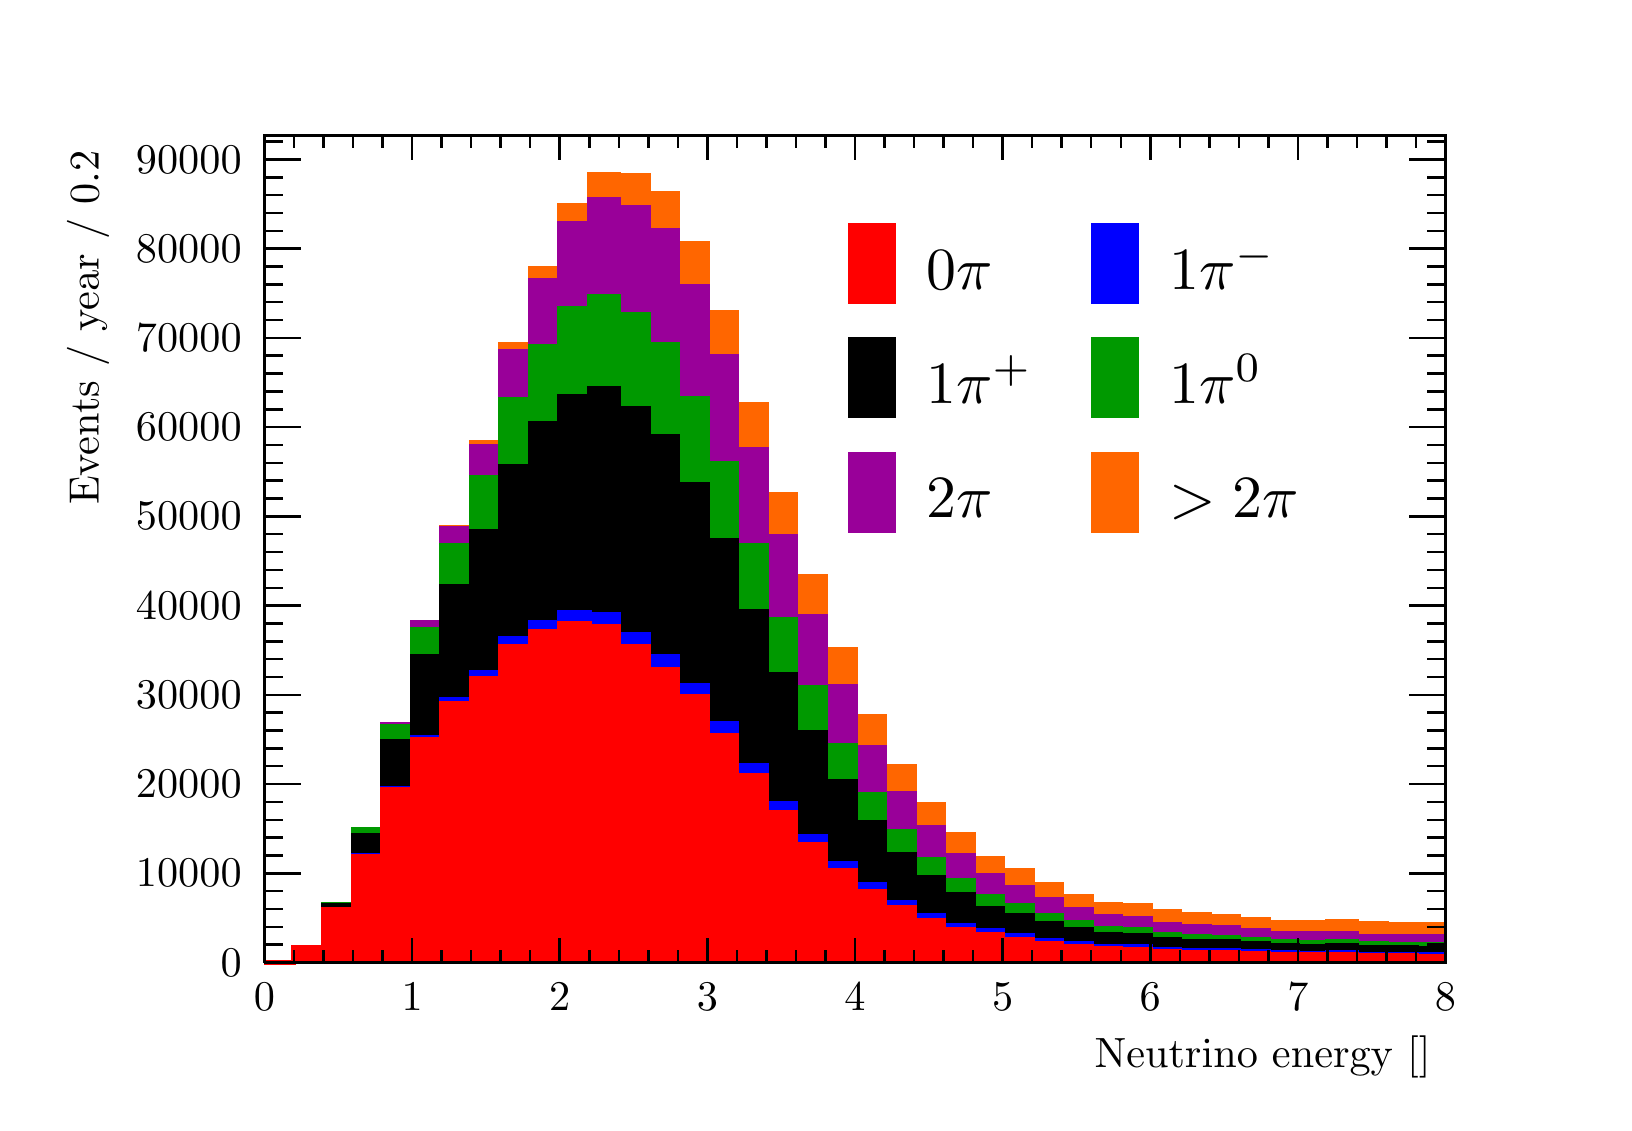
\begin{tikzpicture}
\pgfdeclareplotmark{cross} {
\pgfpathmoveto{\pgfpoint{-0.3\pgfplotmarksize}{\pgfplotmarksize}}
\pgfpathlineto{\pgfpoint{+0.3\pgfplotmarksize}{\pgfplotmarksize}}
\pgfpathlineto{\pgfpoint{+0.3\pgfplotmarksize}{0.3\pgfplotmarksize}}
\pgfpathlineto{\pgfpoint{+1\pgfplotmarksize}{0.3\pgfplotmarksize}}
\pgfpathlineto{\pgfpoint{+1\pgfplotmarksize}{-0.3\pgfplotmarksize}}
\pgfpathlineto{\pgfpoint{+0.3\pgfplotmarksize}{-0.3\pgfplotmarksize}}
\pgfpathlineto{\pgfpoint{+0.3\pgfplotmarksize}{-1.\pgfplotmarksize}}
\pgfpathlineto{\pgfpoint{-0.3\pgfplotmarksize}{-1.\pgfplotmarksize}}
\pgfpathlineto{\pgfpoint{-0.3\pgfplotmarksize}{-0.3\pgfplotmarksize}}
\pgfpathlineto{\pgfpoint{-1.\pgfplotmarksize}{-0.3\pgfplotmarksize}}
\pgfpathlineto{\pgfpoint{-1.\pgfplotmarksize}{0.3\pgfplotmarksize}}
\pgfpathlineto{\pgfpoint{-0.3\pgfplotmarksize}{0.3\pgfplotmarksize}}
\pgfpathclose
\pgfusepathqstroke
}
\pgfdeclareplotmark{cross*} {
\pgfpathmoveto{\pgfpoint{-0.3\pgfplotmarksize}{\pgfplotmarksize}}
\pgfpathlineto{\pgfpoint{+0.3\pgfplotmarksize}{\pgfplotmarksize}}
\pgfpathlineto{\pgfpoint{+0.3\pgfplotmarksize}{0.3\pgfplotmarksize}}
\pgfpathlineto{\pgfpoint{+1\pgfplotmarksize}{0.3\pgfplotmarksize}}
\pgfpathlineto{\pgfpoint{+1\pgfplotmarksize}{-0.3\pgfplotmarksize}}
\pgfpathlineto{\pgfpoint{+0.3\pgfplotmarksize}{-0.3\pgfplotmarksize}}
\pgfpathlineto{\pgfpoint{+0.3\pgfplotmarksize}{-1.\pgfplotmarksize}}
\pgfpathlineto{\pgfpoint{-0.3\pgfplotmarksize}{-1.\pgfplotmarksize}}
\pgfpathlineto{\pgfpoint{-0.3\pgfplotmarksize}{-0.3\pgfplotmarksize}}
\pgfpathlineto{\pgfpoint{-1.\pgfplotmarksize}{-0.3\pgfplotmarksize}}
\pgfpathlineto{\pgfpoint{-1.\pgfplotmarksize}{0.3\pgfplotmarksize}}
\pgfpathlineto{\pgfpoint{-0.3\pgfplotmarksize}{0.3\pgfplotmarksize}}
\pgfpathclose
\pgfusepathqfillstroke
}
\pgfdeclareplotmark{newstar} {
\pgfpathmoveto{\pgfqpoint{0pt}{\pgfplotmarksize}}
\pgfpathlineto{\pgfqpointpolar{44}{0.5\pgfplotmarksize}}
\pgfpathlineto{\pgfqpointpolar{18}{\pgfplotmarksize}}
\pgfpathlineto{\pgfqpointpolar{-20}{0.5\pgfplotmarksize}}
\pgfpathlineto{\pgfqpointpolar{-54}{\pgfplotmarksize}}
\pgfpathlineto{\pgfqpointpolar{-90}{0.5\pgfplotmarksize}}
\pgfpathlineto{\pgfqpointpolar{234}{\pgfplotmarksize}}
\pgfpathlineto{\pgfqpointpolar{198}{0.5\pgfplotmarksize}}
\pgfpathlineto{\pgfqpointpolar{162}{\pgfplotmarksize}}
\pgfpathlineto{\pgfqpointpolar{134}{0.5\pgfplotmarksize}}
\pgfpathclose
\pgfusepathqstroke
}
\pgfdeclareplotmark{newstar*} {
\pgfpathmoveto{\pgfqpoint{0pt}{\pgfplotmarksize}}
\pgfpathlineto{\pgfqpointpolar{44}{0.5\pgfplotmarksize}}
\pgfpathlineto{\pgfqpointpolar{18}{\pgfplotmarksize}}
\pgfpathlineto{\pgfqpointpolar{-20}{0.5\pgfplotmarksize}}
\pgfpathlineto{\pgfqpointpolar{-54}{\pgfplotmarksize}}
\pgfpathlineto{\pgfqpointpolar{-90}{0.5\pgfplotmarksize}}
\pgfpathlineto{\pgfqpointpolar{234}{\pgfplotmarksize}}
\pgfpathlineto{\pgfqpointpolar{198}{0.5\pgfplotmarksize}}
\pgfpathlineto{\pgfqpointpolar{162}{\pgfplotmarksize}}
\pgfpathlineto{\pgfqpointpolar{134}{0.5\pgfplotmarksize}}
\pgfpathclose
\pgfusepathqfillstroke
}
\definecolor{c}{rgb}{1,1,1};
\draw [color=c, fill=c] (0,0) rectangle (20,13.639);
\draw [color=c, fill=c] (3,1.77307) rectangle (18,12.2751);
\definecolor{c}{rgb}{0,0,0};
\draw [c,line width=0.9] (3,1.77307) -- (3,12.2751) -- (18,12.2751) -- (18,1.77307) -- (3,1.77307);
\definecolor{c}{rgb}{1,1,1};
\draw [color=c, fill=c] (3,1.77307) rectangle (18,12.2751);
\definecolor{c}{rgb}{0,0,0};
\draw [c,line width=0.9] (3,1.77307) -- (3,12.2751) -- (18,12.2751) -- (18,1.77307) -- (3,1.77307);
\draw [c,line width=0.9] (3,1.77307) -- (3.375,1.77307) -- (3.375,1.77307) -- (3.75,1.77307) -- (3.75,1.77307) -- (4.125,1.77307) -- (4.125,1.77307) -- (4.5,1.77307) -- (4.5,1.77307) -- (4.875,1.77307) -- (4.875,1.77307) -- (5.25,1.77307) --
 (5.25,1.77307) -- (5.625,1.77307) -- (5.625,1.77307) -- (6,1.77307) -- (6,1.77307) -- (6.375,1.77307) -- (6.375,1.77307) -- (6.75,1.77307) -- (6.75,1.77307) -- (7.125,1.77307) -- (7.125,1.77307) -- (7.5,1.77307) -- (7.5,1.77307) -- (7.875,1.77307)
 -- (7.875,1.77307) -- (8.25,1.77307) -- (8.25,1.77307) -- (8.625,1.77307) -- (8.625,1.77307) -- (9,1.77307) -- (9,1.77307) -- (9.375,1.77307) -- (9.375,1.77307) -- (9.75,1.77307) -- (9.75,1.77307) -- (10.125,1.77307) -- (10.125,1.77307) --
 (10.5,1.77307) -- (10.5,1.77307) -- (10.875,1.77307) -- (10.875,1.77307) -- (11.25,1.77307) -- (11.25,1.77307) -- (11.625,1.77307) -- (11.625,1.77307) -- (12,1.77307) -- (12,1.77307) -- (12.375,1.77307) -- (12.375,1.77307) -- (12.75,1.77307) --
 (12.75,1.77307) -- (13.125,1.77307) -- (13.125,1.77307) -- (13.5,1.77307) -- (13.5,1.77307) -- (13.875,1.77307) -- (13.875,1.77307) -- (14.25,1.77307) -- (14.25,1.77307) -- (14.625,1.77307) -- (14.625,1.77307) -- (15,1.77307) -- (15,1.77307) --
 (15.375,1.77307) -- (15.375,1.77307) -- (15.75,1.77307) -- (15.75,1.77307) -- (16.125,1.77307) -- (16.125,1.77307) -- (16.5,1.77307) -- (16.5,1.77307) -- (16.875,1.77307) -- (16.875,1.77307) -- (17.25,1.77307) -- (17.25,1.77307) -- (17.625,1.77307)
 -- (17.625,1.77307) -- (18,1.77307);
\draw [c,line width=0.9] (3,1.77307) -- (18,1.77307);
\draw [c,line width=0.9] (3,2.07994) -- (3,1.77307);
\draw [c,line width=0.9] (3.375,1.9265) -- (3.375,1.77307);
\draw [c,line width=0.9] (3.75,1.9265) -- (3.75,1.77307);
\draw [c,line width=0.9] (4.125,1.9265) -- (4.125,1.77307);
\draw [c,line width=0.9] (4.5,1.9265) -- (4.5,1.77307);
\draw [c,line width=0.9] (4.875,2.07994) -- (4.875,1.77307);
\draw [c,line width=0.9] (5.25,1.9265) -- (5.25,1.77307);
\draw [c,line width=0.9] (5.625,1.9265) -- (5.625,1.77307);
\draw [c,line width=0.9] (6,1.9265) -- (6,1.77307);
\draw [c,line width=0.9] (6.375,1.9265) -- (6.375,1.77307);
\draw [c,line width=0.9] (6.75,2.07994) -- (6.75,1.77307);
\draw [c,line width=0.9] (7.125,1.9265) -- (7.125,1.77307);
\draw [c,line width=0.9] (7.5,1.9265) -- (7.5,1.77307);
\draw [c,line width=0.9] (7.875,1.9265) -- (7.875,1.77307);
\draw [c,line width=0.9] (8.25,1.9265) -- (8.25,1.77307);
\draw [c,line width=0.9] (8.625,2.07994) -- (8.625,1.77307);
\draw [c,line width=0.9] (9,1.9265) -- (9,1.77307);
\draw [c,line width=0.9] (9.375,1.9265) -- (9.375,1.77307);
\draw [c,line width=0.9] (9.75,1.9265) -- (9.75,1.77307);
\draw [c,line width=0.9] (10.125,1.9265) -- (10.125,1.77307);
\draw [c,line width=0.9] (10.5,2.07994) -- (10.5,1.77307);
\draw [c,line width=0.9] (10.875,1.9265) -- (10.875,1.77307);
\draw [c,line width=0.9] (11.25,1.9265) -- (11.25,1.77307);
\draw [c,line width=0.9] (11.625,1.9265) -- (11.625,1.77307);
\draw [c,line width=0.9] (12,1.9265) -- (12,1.77307);
\draw [c,line width=0.9] (12.375,2.07994) -- (12.375,1.77307);
\draw [c,line width=0.9] (12.75,1.9265) -- (12.75,1.77307);
\draw [c,line width=0.9] (13.125,1.9265) -- (13.125,1.77307);
\draw [c,line width=0.9] (13.5,1.9265) -- (13.5,1.77307);
\draw [c,line width=0.9] (13.875,1.9265) -- (13.875,1.77307);
\draw [c,line width=0.9] (14.25,2.07994) -- (14.25,1.77307);
\draw [c,line width=0.9] (14.625,1.9265) -- (14.625,1.77307);
\draw [c,line width=0.9] (15,1.9265) -- (15,1.77307);
\draw [c,line width=0.9] (15.375,1.9265) -- (15.375,1.77307);
\draw [c,line width=0.9] (15.75,1.9265) -- (15.75,1.77307);
\draw [c,line width=0.9] (16.125,2.07994) -- (16.125,1.77307);
\draw [c,line width=0.9] (16.5,1.9265) -- (16.5,1.77307);
\draw [c,line width=0.9] (16.875,1.9265) -- (16.875,1.77307);
\draw [c,line width=0.9] (17.25,1.9265) -- (17.25,1.77307);
\draw [c,line width=0.9] (17.625,1.9265) -- (17.625,1.77307);
\draw [c,line width=0.9] (18,2.07994) -- (18,1.77307);
\draw [anchor=base] (3,1.15931) node[scale=1.52731, color=c, rotate=0]{0};
\draw [anchor=base] (4.875,1.15931) node[scale=1.52731, color=c, rotate=0]{1};
\draw [anchor=base] (6.75,1.15931) node[scale=1.52731, color=c, rotate=0]{2};
\draw [anchor=base] (8.625,1.15931) node[scale=1.52731, color=c, rotate=0]{3};
\draw [anchor=base] (10.5,1.15931) node[scale=1.52731, color=c, rotate=0]{4};
\draw [anchor=base] (12.375,1.15931) node[scale=1.52731, color=c, rotate=0]{5};
\draw [anchor=base] (14.25,1.15931) node[scale=1.52731, color=c, rotate=0]{6};
\draw [anchor=base] (16.125,1.15931) node[scale=1.52731, color=c, rotate=0]{7};
\draw [anchor=base] (18,1.15931) node[scale=1.52731, color=c, rotate=0]{8};
\draw [anchor= east] (18,0.572837) node[scale=1.52731, color=c, rotate=0]{ Neutrino energy [\si{\giga\electronvolt}]};
\draw [c,line width=0.9] (3,12.2751) -- (18,12.2751);
\draw [c,line width=0.9] (3,11.9682) -- (3,12.2751);
\draw [c,line width=0.9] (3.375,12.1216) -- (3.375,12.2751);
\draw [c,line width=0.9] (3.75,12.1216) -- (3.75,12.2751);
\draw [c,line width=0.9] (4.125,12.1216) -- (4.125,12.2751);
\draw [c,line width=0.9] (4.5,12.1216) -- (4.5,12.2751);
\draw [c,line width=0.9] (4.875,11.9682) -- (4.875,12.2751);
\draw [c,line width=0.9] (5.25,12.1216) -- (5.25,12.2751);
\draw [c,line width=0.9] (5.625,12.1216) -- (5.625,12.2751);
\draw [c,line width=0.9] (6,12.1216) -- (6,12.2751);
\draw [c,line width=0.9] (6.375,12.1216) -- (6.375,12.2751);
\draw [c,line width=0.9] (6.75,11.9682) -- (6.75,12.2751);
\draw [c,line width=0.9] (7.125,12.1216) -- (7.125,12.2751);
\draw [c,line width=0.9] (7.5,12.1216) -- (7.5,12.2751);
\draw [c,line width=0.9] (7.875,12.1216) -- (7.875,12.2751);
\draw [c,line width=0.9] (8.25,12.1216) -- (8.25,12.2751);
\draw [c,line width=0.9] (8.625,11.9682) -- (8.625,12.2751);
\draw [c,line width=0.9] (9,12.1216) -- (9,12.2751);
\draw [c,line width=0.9] (9.375,12.1216) -- (9.375,12.2751);
\draw [c,line width=0.9] (9.75,12.1216) -- (9.75,12.2751);
\draw [c,line width=0.9] (10.125,12.1216) -- (10.125,12.2751);
\draw [c,line width=0.9] (10.5,11.9682) -- (10.5,12.2751);
\draw [c,line width=0.9] (10.875,12.1216) -- (10.875,12.2751);
\draw [c,line width=0.9] (11.25,12.1216) -- (11.25,12.2751);
\draw [c,line width=0.9] (11.625,12.1216) -- (11.625,12.2751);
\draw [c,line width=0.9] (12,12.1216) -- (12,12.2751);
\draw [c,line width=0.9] (12.375,11.9682) -- (12.375,12.2751);
\draw [c,line width=0.9] (12.75,12.1216) -- (12.75,12.2751);
\draw [c,line width=0.9] (13.125,12.1216) -- (13.125,12.2751);
\draw [c,line width=0.9] (13.5,12.1216) -- (13.5,12.2751);
\draw [c,line width=0.9] (13.875,12.1216) -- (13.875,12.2751);
\draw [c,line width=0.9] (14.25,11.9682) -- (14.25,12.2751);
\draw [c,line width=0.9] (14.625,12.1216) -- (14.625,12.2751);
\draw [c,line width=0.9] (15,12.1216) -- (15,12.2751);
\draw [c,line width=0.9] (15.375,12.1216) -- (15.375,12.2751);
\draw [c,line width=0.9] (15.75,12.1216) -- (15.75,12.2751);
\draw [c,line width=0.9] (16.125,11.9682) -- (16.125,12.2751);
\draw [c,line width=0.9] (16.5,12.1216) -- (16.5,12.2751);
\draw [c,line width=0.9] (16.875,12.1216) -- (16.875,12.2751);
\draw [c,line width=0.9] (17.25,12.1216) -- (17.25,12.2751);
\draw [c,line width=0.9] (17.625,12.1216) -- (17.625,12.2751);
\draw [c,line width=0.9] (18,11.9682) -- (18,12.2751);
\draw [c,line width=0.9] (3,1.77307) -- (3,12.2751);
\draw [c,line width=0.9] (3.462,1.77307) -- (3,1.77307);
\draw [c,line width=0.9] (3.231,1.99972) -- (3,1.99972);
\draw [c,line width=0.9] (3.231,2.22638) -- (3,2.22638);
\draw [c,line width=0.9] (3.231,2.45304) -- (3,2.45304);
\draw [c,line width=0.9] (3.231,2.67969) -- (3,2.67969);
\draw [c,line width=0.9] (3.462,2.90635) -- (3,2.90635);
\draw [c,line width=0.9] (3.231,3.13301) -- (3,3.13301);
\draw [c,line width=0.9] (3.231,3.35967) -- (3,3.35967);
\draw [c,line width=0.9] (3.231,3.58632) -- (3,3.58632);
\draw [c,line width=0.9] (3.231,3.81298) -- (3,3.81298);
\draw [c,line width=0.9] (3.462,4.03964) -- (3,4.03964);
\draw [c,line width=0.9] (3.231,4.26629) -- (3,4.26629);
\draw [c,line width=0.9] (3.231,4.49295) -- (3,4.49295);
\draw [c,line width=0.9] (3.231,4.71961) -- (3,4.71961);
\draw [c,line width=0.9] (3.231,4.94626) -- (3,4.94626);
\draw [c,line width=0.9] (3.462,5.17292) -- (3,5.17292);
\draw [c,line width=0.9] (3.231,5.39958) -- (3,5.39958);
\draw [c,line width=0.9] (3.231,5.62624) -- (3,5.62624);
\draw [c,line width=0.9] (3.231,5.85289) -- (3,5.85289);
\draw [c,line width=0.9] (3.231,6.07955) -- (3,6.07955);
\draw [c,line width=0.9] (3.462,6.30621) -- (3,6.30621);
\draw [c,line width=0.9] (3.231,6.53286) -- (3,6.53286);
\draw [c,line width=0.9] (3.231,6.75952) -- (3,6.75952);
\draw [c,line width=0.9] (3.231,6.98618) -- (3,6.98618);
\draw [c,line width=0.9] (3.231,7.21283) -- (3,7.21283);
\draw [c,line width=0.9] (3.462,7.43949) -- (3,7.43949);
\draw [c,line width=0.9] (3.231,7.66615) -- (3,7.66615);
\draw [c,line width=0.9] (3.231,7.89281) -- (3,7.89281);
\draw [c,line width=0.9] (3.231,8.11946) -- (3,8.11946);
\draw [c,line width=0.9] (3.231,8.34612) -- (3,8.34612);
\draw [c,line width=0.9] (3.462,8.57278) -- (3,8.57278);
\draw [c,line width=0.9] (3.231,8.79943) -- (3,8.79943);
\draw [c,line width=0.9] (3.231,9.02609) -- (3,9.02609);
\draw [c,line width=0.9] (3.231,9.25275) -- (3,9.25275);
\draw [c,line width=0.9] (3.231,9.4794) -- (3,9.4794);
\draw [c,line width=0.9] (3.462,9.70606) -- (3,9.70606);
\draw [c,line width=0.9] (3.231,9.93272) -- (3,9.93272);
\draw [c,line width=0.9] (3.231,10.1594) -- (3,10.1594);
\draw [c,line width=0.9] (3.231,10.386) -- (3,10.386);
\draw [c,line width=0.9] (3.231,10.6127) -- (3,10.6127);
\draw [c,line width=0.9] (3.462,10.8393) -- (3,10.8393);
\draw [c,line width=0.9] (3.231,11.066) -- (3,11.066);
\draw [c,line width=0.9] (3.231,11.2927) -- (3,11.2927);
\draw [c,line width=0.9] (3.231,11.5193) -- (3,11.5193);
\draw [c,line width=0.9] (3.231,11.746) -- (3,11.746);
\draw [c,line width=0.9] (3.462,11.9726) -- (3,11.9726);
\draw [c,line width=0.9] (3.462,11.9726) -- (3,11.9726);
\draw [c,line width=0.9] (3.231,12.1993) -- (3,12.1993);
\draw [anchor= east] (2.9,1.77307) node[scale=1.52731, color=c, rotate=0]{0};
\draw [anchor= east] (2.9,2.90635) node[scale=1.52731, color=c, rotate=0]{10000};
\draw [anchor= east] (2.9,4.03964) node[scale=1.52731, color=c, rotate=0]{20000};
\draw [anchor= east] (2.9,5.17292) node[scale=1.52731, color=c, rotate=0]{30000};
\draw [anchor= east] (2.9,6.30621) node[scale=1.52731, color=c, rotate=0]{40000};
\draw [anchor= east] (2.9,7.43949) node[scale=1.52731, color=c, rotate=0]{50000};
\draw [anchor= east] (2.9,8.57278) node[scale=1.52731, color=c, rotate=0]{60000};
\draw [anchor= east] (2.9,9.70606) node[scale=1.52731, color=c, rotate=0]{70000};
\draw [anchor= east] (2.9,10.8393) node[scale=1.52731, color=c, rotate=0]{80000};
\draw [anchor= east] (2.9,11.9726) node[scale=1.52731, color=c, rotate=0]{90000};
\draw [anchor= east] (0.76,12.2751) node[scale=1.52731, color=c, rotate=90]{ Events / year / \SI{0.2}{\giga\electronvolt} };
\draw [c,line width=0.9] (18,1.77307) -- (18,12.2751);
\draw [c,line width=0.9] (17.538,1.77307) -- (18,1.77307);
\draw [c,line width=0.9] (17.769,1.99972) -- (18,1.99972);
\draw [c,line width=0.9] (17.769,2.22638) -- (18,2.22638);
\draw [c,line width=0.9] (17.769,2.45304) -- (18,2.45304);
\draw [c,line width=0.9] (17.769,2.67969) -- (18,2.67969);
\draw [c,line width=0.9] (17.538,2.90635) -- (18,2.90635);
\draw [c,line width=0.9] (17.769,3.13301) -- (18,3.13301);
\draw [c,line width=0.9] (17.769,3.35967) -- (18,3.35967);
\draw [c,line width=0.9] (17.769,3.58632) -- (18,3.58632);
\draw [c,line width=0.9] (17.769,3.81298) -- (18,3.81298);
\draw [c,line width=0.9] (17.538,4.03964) -- (18,4.03964);
\draw [c,line width=0.9] (17.769,4.26629) -- (18,4.26629);
\draw [c,line width=0.9] (17.769,4.49295) -- (18,4.49295);
\draw [c,line width=0.9] (17.769,4.71961) -- (18,4.71961);
\draw [c,line width=0.9] (17.769,4.94626) -- (18,4.94626);
\draw [c,line width=0.9] (17.538,5.17292) -- (18,5.17292);
\draw [c,line width=0.9] (17.769,5.39958) -- (18,5.39958);
\draw [c,line width=0.9] (17.769,5.62624) -- (18,5.62624);
\draw [c,line width=0.9] (17.769,5.85289) -- (18,5.85289);
\draw [c,line width=0.9] (17.769,6.07955) -- (18,6.07955);
\draw [c,line width=0.9] (17.538,6.30621) -- (18,6.30621);
\draw [c,line width=0.9] (17.769,6.53286) -- (18,6.53286);
\draw [c,line width=0.9] (17.769,6.75952) -- (18,6.75952);
\draw [c,line width=0.9] (17.769,6.98618) -- (18,6.98618);
\draw [c,line width=0.9] (17.769,7.21283) -- (18,7.21283);
\draw [c,line width=0.9] (17.538,7.43949) -- (18,7.43949);
\draw [c,line width=0.9] (17.769,7.66615) -- (18,7.66615);
\draw [c,line width=0.9] (17.769,7.89281) -- (18,7.89281);
\draw [c,line width=0.9] (17.769,8.11946) -- (18,8.11946);
\draw [c,line width=0.9] (17.769,8.34612) -- (18,8.34612);
\draw [c,line width=0.9] (17.538,8.57278) -- (18,8.57278);
\draw [c,line width=0.9] (17.769,8.79943) -- (18,8.79943);
\draw [c,line width=0.9] (17.769,9.02609) -- (18,9.02609);
\draw [c,line width=0.9] (17.769,9.25275) -- (18,9.25275);
\draw [c,line width=0.9] (17.769,9.4794) -- (18,9.4794);
\draw [c,line width=0.9] (17.538,9.70606) -- (18,9.70606);
\draw [c,line width=0.9] (17.769,9.93272) -- (18,9.93272);
\draw [c,line width=0.9] (17.769,10.1594) -- (18,10.1594);
\draw [c,line width=0.9] (17.769,10.386) -- (18,10.386);
\draw [c,line width=0.9] (17.769,10.6127) -- (18,10.6127);
\draw [c,line width=0.9] (17.538,10.8393) -- (18,10.8393);
\draw [c,line width=0.9] (17.769,11.066) -- (18,11.066);
\draw [c,line width=0.9] (17.769,11.2927) -- (18,11.2927);
\draw [c,line width=0.9] (17.769,11.5193) -- (18,11.5193);
\draw [c,line width=0.9] (17.769,11.746) -- (18,11.746);
\draw [c,line width=0.9] (17.538,11.9726) -- (18,11.9726);
\draw [c,line width=0.9] (17.538,11.9726) -- (18,11.9726);
\draw [c,line width=0.9] (17.769,12.1993) -- (18,12.1993);
\definecolor{c}{rgb}{1,0.4,0};
\draw [c, fill=c] (3,1.77307) -- (3,1.779) -- (3.375,1.779) -- (3.375,1.95842) -- (3.75,1.95842) -- (3.75,2.50479) -- (4.125,2.50479) -- (4.125,3.46262) -- (4.5,3.46262) -- (4.5,4.79128) -- (4.875,4.79128) -- (4.875,6.09505) -- (5.25,6.09505) --
 (5.25,7.29305) -- (5.625,7.29305) -- (5.625,8.37548) -- (6,8.37548) -- (6,9.61824) -- (6.375,9.61824) -- (6.375,10.5866) -- (6.75,10.5866) -- (6.75,11.3838) -- (7.125,11.3838) -- (7.125,11.775) -- (7.5,11.775) -- (7.5,11.7652) -- (7.875,11.7652) --
 (7.875,11.5346) -- (8.25,11.5346) -- (8.25,10.8989) -- (8.625,10.8989) -- (8.625,10.0316) -- (9,10.0316) -- (9,8.85685) -- (9.375,8.85685) -- (9.375,7.71973) -- (9.75,7.71973) -- (9.75,6.67058) -- (10.125,6.67058) -- (10.125,5.74628) --
 (10.5,5.74628) -- (10.5,4.90157) -- (10.875,4.90157) -- (10.875,4.25819) -- (11.25,4.25819) -- (11.25,3.77863) -- (11.625,3.77863) -- (11.625,3.39323) -- (12,3.39323) -- (12,3.10044) -- (12.375,3.10044) -- (12.375,2.94088) -- (12.75,2.94088) --
 (12.75,2.76379) -- (13.125,2.76379) -- (13.125,2.61198) -- (13.5,2.61198) -- (13.5,2.51279) -- (13.875,2.51279) -- (13.875,2.49138) -- (14.25,2.49138) -- (14.25,2.41618) -- (14.625,2.41618) -- (14.625,2.38277) -- (15,2.38277) -- (15,2.35543) --
 (15.375,2.35543) -- (15.375,2.32473) -- (15.75,2.32473) -- (15.75,2.27584) -- (16.125,2.27584) -- (16.125,2.28255) -- (16.5,2.28255) -- (16.5,2.29042) -- (16.875,2.29042) -- (16.875,2.2654) -- (17.25,2.2654) -- (17.25,2.25147) -- (17.625,2.25147) --
 (17.625,2.25959) -- (18,2.25959) -- (18,1.77307);
\draw [c,line width=1.8] (3,1.779) -- (3.375,1.779) -- (3.375,1.95842) -- (3.75,1.95842) -- (3.75,2.50479) -- (4.125,2.50479) -- (4.125,3.46262) -- (4.5,3.46262) -- (4.5,4.79128) -- (4.875,4.79128) -- (4.875,6.09505) -- (5.25,6.09505) --
 (5.25,7.29305) -- (5.625,7.29305) -- (5.625,8.37548) -- (6,8.37548) -- (6,9.61824) -- (6.375,9.61824) -- (6.375,10.5866) -- (6.75,10.5866) -- (6.75,11.3838) -- (7.125,11.3838) -- (7.125,11.775) -- (7.5,11.775) -- (7.5,11.7652) -- (7.875,11.7652) --
 (7.875,11.5346) -- (8.25,11.5346) -- (8.25,10.8989) -- (8.625,10.8989) -- (8.625,10.0316) -- (9,10.0316) -- (9,8.85685) -- (9.375,8.85685) -- (9.375,7.71973) -- (9.75,7.71973) -- (9.75,6.67058) -- (10.125,6.67058) -- (10.125,5.74628) --
 (10.5,5.74628) -- (10.5,4.90157) -- (10.875,4.90157) -- (10.875,4.25819) -- (11.25,4.25819) -- (11.25,3.77863) -- (11.625,3.77863) -- (11.625,3.39323) -- (12,3.39323) -- (12,3.10044) -- (12.375,3.10044) -- (12.375,2.94088) -- (12.75,2.94088) --
 (12.75,2.76379) -- (13.125,2.76379) -- (13.125,2.61198) -- (13.5,2.61198) -- (13.5,2.51279) -- (13.875,2.51279) -- (13.875,2.49138) -- (14.25,2.49138) -- (14.25,2.41618) -- (14.625,2.41618) -- (14.625,2.38277) -- (15,2.38277) -- (15,2.35543) --
 (15.375,2.35543) -- (15.375,2.32473) -- (15.75,2.32473) -- (15.75,2.27584) -- (16.125,2.27584) -- (16.125,2.28255) -- (16.5,2.28255) -- (16.5,2.29042) -- (16.875,2.29042) -- (16.875,2.2654) -- (17.25,2.2654) -- (17.25,2.25147) -- (17.625,2.25147) --
 (17.625,2.25959) -- (18,2.25959);
\definecolor{c}{rgb}{0.999,0.999,0.999};
\draw [c, fill=c] (3,1.77307) -- (3,1.779) -- (3.375,1.779) -- (3.375,1.95842) -- (3.75,1.95842) -- (3.75,2.50479) -- (4.125,2.50479) -- (4.125,3.46262) -- (4.5,3.46262) -- (4.5,4.79038) -- (4.875,4.79038) -- (4.875,6.09054) -- (5.25,6.09054) --
 (5.25,7.27977) -- (5.625,7.27977) -- (5.625,8.33189) -- (6,8.33189) -- (6,9.53569) -- (6.375,9.53569) -- (6.375,10.4404) -- (6.75,10.4404) -- (6.75,11.16) -- (7.125,11.16) -- (7.125,11.4684) -- (7.5,11.4684) -- (7.5,11.3638) -- (7.875,11.3638) --
 (7.875,11.0662) -- (8.25,11.0662) -- (8.25,10.3595) -- (8.625,10.3595) -- (8.625,9.46784) -- (9,9.46784) -- (9,8.28687) -- (9.375,8.28687) -- (9.375,7.18148) -- (9.75,7.18148) -- (9.75,6.17193) -- (10.125,6.17193) -- (10.125,5.28207) --
 (10.5,5.28207) -- (10.5,4.51023) -- (10.875,4.51023) -- (10.875,3.92632) -- (11.25,3.92632) -- (11.25,3.48997) -- (11.625,3.48997) -- (11.625,3.13707) -- (12,3.13707) -- (12,2.87768) -- (12.375,2.87768) -- (12.375,2.7318) -- (12.75,2.7318) --
 (12.75,2.56993) -- (13.125,2.56993) -- (13.125,2.44688) -- (13.5,2.44688) -- (13.5,2.35517) -- (13.875,2.35517) -- (13.875,2.3384) -- (14.25,2.3384) -- (14.25,2.26191) -- (14.625,2.26191) -- (14.625,2.23199) -- (15,2.23199) -- (15,2.21393) --
 (15.375,2.21393) -- (15.375,2.17911) -- (15.75,2.17911) -- (15.75,2.14144) -- (16.125,2.14144) -- (16.125,2.13835) -- (16.5,2.13835) -- (16.5,2.1448) -- (16.875,2.1448) -- (16.875,2.10804) -- (17.25,2.10804) -- (17.25,2.10417) -- (17.625,2.10417) --
 (17.625,2.10726) -- (18,2.10726) -- (18,1.77307);
\definecolor{c}{rgb}{0.6,0,0.6};
\draw [c,line width=1.8] (3,1.779) -- (3.375,1.779) -- (3.375,1.95842) -- (3.75,1.95842) -- (3.75,2.50479) -- (4.125,2.50479) -- (4.125,3.46262) -- (4.5,3.46262) -- (4.5,4.79038) -- (4.875,4.79038) -- (4.875,6.09054) -- (5.25,6.09054) --
 (5.25,7.27977) -- (5.625,7.27977) -- (5.625,8.33189) -- (6,8.33189) -- (6,9.53569) -- (6.375,9.53569) -- (6.375,10.4404) -- (6.75,10.4404) -- (6.75,11.16) -- (7.125,11.16) -- (7.125,11.4684) -- (7.5,11.4684) -- (7.5,11.3638) -- (7.875,11.3638) --
 (7.875,11.0662) -- (8.25,11.0662) -- (8.25,10.3595) -- (8.625,10.3595) -- (8.625,9.46784) -- (9,9.46784) -- (9,8.28687) -- (9.375,8.28687) -- (9.375,7.18148) -- (9.75,7.18148) -- (9.75,6.17193) -- (10.125,6.17193) -- (10.125,5.28207) --
 (10.5,5.28207) -- (10.5,4.51023) -- (10.875,4.51023) -- (10.875,3.92632) -- (11.25,3.92632) -- (11.25,3.48997) -- (11.625,3.48997) -- (11.625,3.13707) -- (12,3.13707) -- (12,2.87768) -- (12.375,2.87768) -- (12.375,2.7318) -- (12.75,2.7318) --
 (12.75,2.56993) -- (13.125,2.56993) -- (13.125,2.44688) -- (13.5,2.44688) -- (13.5,2.35517) -- (13.875,2.35517) -- (13.875,2.3384) -- (14.25,2.3384) -- (14.25,2.26191) -- (14.625,2.26191) -- (14.625,2.23199) -- (15,2.23199) -- (15,2.21393) --
 (15.375,2.21393) -- (15.375,2.17911) -- (15.75,2.17911) -- (15.75,2.14144) -- (16.125,2.14144) -- (16.125,2.13835) -- (16.5,2.13835) -- (16.5,2.1448) -- (16.875,2.1448) -- (16.875,2.10804) -- (17.25,2.10804) -- (17.25,2.10417) -- (17.625,2.10417) --
 (17.625,2.10726) -- (18,2.10726);
\draw [c,line width=1.8] (3,1.779) -- (3.375,1.779) -- (3.375,1.95842) -- (3.75,1.95842) -- (3.75,2.50479) -- (4.125,2.50479) -- (4.125,3.46262) -- (4.5,3.46262) -- (4.5,4.79038) -- (4.875,4.79038) -- (4.875,6.09054) -- (5.25,6.09054) --
 (5.25,7.27977) -- (5.625,7.27977) -- (5.625,8.33189) -- (6,8.33189) -- (6,9.53569) -- (6.375,9.53569) -- (6.375,10.4404) -- (6.75,10.4404) -- (6.75,11.16) -- (7.125,11.16) -- (7.125,11.4684) -- (7.5,11.4684) -- (7.5,11.3638) -- (7.875,11.3638) --
 (7.875,11.0662) -- (8.25,11.0662) -- (8.25,10.3595) -- (8.625,10.3595) -- (8.625,9.46784) -- (9,9.46784) -- (9,8.28687) -- (9.375,8.28687) -- (9.375,7.18148) -- (9.75,7.18148) -- (9.75,6.17193) -- (10.125,6.17193) -- (10.125,5.28207) --
 (10.5,5.28207) -- (10.5,4.51023) -- (10.875,4.51023) -- (10.875,3.92632) -- (11.25,3.92632) -- (11.25,3.48997) -- (11.625,3.48997) -- (11.625,3.13707) -- (12,3.13707) -- (12,2.87768) -- (12.375,2.87768) -- (12.375,2.7318) -- (12.75,2.7318) --
 (12.75,2.56993) -- (13.125,2.56993) -- (13.125,2.44688) -- (13.5,2.44688) -- (13.5,2.35517) -- (13.875,2.35517) -- (13.875,2.3384) -- (14.25,2.3384) -- (14.25,2.26191) -- (14.625,2.26191) -- (14.625,2.23199) -- (15,2.23199) -- (15,2.21393) --
 (15.375,2.21393) -- (15.375,2.17911) -- (15.75,2.17911) -- (15.75,2.14144) -- (16.125,2.14144) -- (16.125,2.13835) -- (16.5,2.13835) -- (16.5,2.1448) -- (16.875,2.1448) -- (16.875,2.10804) -- (17.25,2.10804) -- (17.25,2.10417) -- (17.625,2.10417) --
 (17.625,2.10726) -- (18,2.10726);
\draw [c, fill=c] (3,1.77307) -- (3,1.779) -- (3.375,1.779) -- (3.375,1.95842) -- (3.75,1.95842) -- (3.75,2.50479) -- (4.125,2.50479) -- (4.125,3.46262) -- (4.5,3.46262) -- (4.5,4.79038) -- (4.875,4.79038) -- (4.875,6.09054) -- (5.25,6.09054) --
 (5.25,7.27977) -- (5.625,7.27977) -- (5.625,8.33189) -- (6,8.33189) -- (6,9.53569) -- (6.375,9.53569) -- (6.375,10.4404) -- (6.75,10.4404) -- (6.75,11.16) -- (7.125,11.16) -- (7.125,11.4684) -- (7.5,11.4684) -- (7.5,11.3638) -- (7.875,11.3638) --
 (7.875,11.0662) -- (8.25,11.0662) -- (8.25,10.3595) -- (8.625,10.3595) -- (8.625,9.46784) -- (9,9.46784) -- (9,8.28687) -- (9.375,8.28687) -- (9.375,7.18148) -- (9.75,7.18148) -- (9.75,6.17193) -- (10.125,6.17193) -- (10.125,5.28207) --
 (10.5,5.28207) -- (10.5,4.51023) -- (10.875,4.51023) -- (10.875,3.92632) -- (11.25,3.92632) -- (11.25,3.48997) -- (11.625,3.48997) -- (11.625,3.13707) -- (12,3.13707) -- (12,2.87768) -- (12.375,2.87768) -- (12.375,2.7318) -- (12.75,2.7318) --
 (12.75,2.56993) -- (13.125,2.56993) -- (13.125,2.44688) -- (13.5,2.44688) -- (13.5,2.35517) -- (13.875,2.35517) -- (13.875,2.3384) -- (14.25,2.3384) -- (14.25,2.26191) -- (14.625,2.26191) -- (14.625,2.23199) -- (15,2.23199) -- (15,2.21393) --
 (15.375,2.21393) -- (15.375,2.17911) -- (15.75,2.17911) -- (15.75,2.14144) -- (16.125,2.14144) -- (16.125,2.13835) -- (16.5,2.13835) -- (16.5,2.1448) -- (16.875,2.1448) -- (16.875,2.10804) -- (17.25,2.10804) -- (17.25,2.10417) -- (17.625,2.10417) --
 (17.625,2.10726) -- (18,2.10726) -- (18,1.77307);
\draw [c,line width=1.8] (3,1.779) -- (3.375,1.779) -- (3.375,1.95842) -- (3.75,1.95842) -- (3.75,2.50479) -- (4.125,2.50479) -- (4.125,3.46262) -- (4.5,3.46262) -- (4.5,4.79038) -- (4.875,4.79038) -- (4.875,6.09054) -- (5.25,6.09054) --
 (5.25,7.27977) -- (5.625,7.27977) -- (5.625,8.33189) -- (6,8.33189) -- (6,9.53569) -- (6.375,9.53569) -- (6.375,10.4404) -- (6.75,10.4404) -- (6.75,11.16) -- (7.125,11.16) -- (7.125,11.4684) -- (7.5,11.4684) -- (7.5,11.3638) -- (7.875,11.3638) --
 (7.875,11.0662) -- (8.25,11.0662) -- (8.25,10.3595) -- (8.625,10.3595) -- (8.625,9.46784) -- (9,9.46784) -- (9,8.28687) -- (9.375,8.28687) -- (9.375,7.18148) -- (9.75,7.18148) -- (9.75,6.17193) -- (10.125,6.17193) -- (10.125,5.28207) --
 (10.5,5.28207) -- (10.5,4.51023) -- (10.875,4.51023) -- (10.875,3.92632) -- (11.25,3.92632) -- (11.25,3.48997) -- (11.625,3.48997) -- (11.625,3.13707) -- (12,3.13707) -- (12,2.87768) -- (12.375,2.87768) -- (12.375,2.7318) -- (12.75,2.7318) --
 (12.75,2.56993) -- (13.125,2.56993) -- (13.125,2.44688) -- (13.5,2.44688) -- (13.5,2.35517) -- (13.875,2.35517) -- (13.875,2.3384) -- (14.25,2.3384) -- (14.25,2.26191) -- (14.625,2.26191) -- (14.625,2.23199) -- (15,2.23199) -- (15,2.21393) --
 (15.375,2.21393) -- (15.375,2.17911) -- (15.75,2.17911) -- (15.75,2.14144) -- (16.125,2.14144) -- (16.125,2.13835) -- (16.5,2.13835) -- (16.5,2.1448) -- (16.875,2.1448) -- (16.875,2.10804) -- (17.25,2.10804) -- (17.25,2.10417) -- (17.625,2.10417) --
 (17.625,2.10726) -- (18,2.10726);
\definecolor{c}{rgb}{0.999,0.999,0.999};
\draw [c, fill=c] (3,1.77307) -- (3,1.779) -- (3.375,1.779) -- (3.375,1.95842) -- (3.75,1.95842) -- (3.75,2.50479) -- (4.125,2.50479) -- (4.125,3.46133) -- (4.5,3.46133) -- (4.5,4.77581) -- (4.875,4.77581) -- (4.875,6.00812) -- (5.25,6.00812) --
 (5.25,7.06501) -- (5.625,7.06501) -- (5.625,7.93603) -- (6,7.93603) -- (6,8.91954) -- (6.375,8.91954) -- (6.375,9.59373) -- (6.75,9.59373) -- (6.75,10.0792) -- (7.125,10.0792) -- (7.125,10.2305) -- (7.5,10.2305) -- (7.5,10.0021) -- (7.875,10.0021)
 -- (7.875,9.61682) -- (8.25,9.61682) -- (8.25,8.93114) -- (8.625,8.93114) -- (8.625,8.11119) -- (9,8.11119) -- (9,7.07004) -- (9.375,7.07004) -- (9.375,6.12975) -- (9.75,6.12975) -- (9.75,5.26478) -- (10.125,5.26478) -- (10.125,4.53035) --
 (10.5,4.53035) -- (10.5,3.90401) -- (10.875,3.90401) -- (10.875,3.43579) -- (11.25,3.43579) -- (11.25,3.07774) -- (11.625,3.07774) -- (11.625,2.80984) -- (12,2.80984) -- (12,2.60759) -- (12.375,2.60759) -- (12.375,2.49654) -- (12.75,2.49654) --
 (12.75,2.37078) -- (13.125,2.37078) -- (13.125,2.27559) -- (13.5,2.27559) -- (13.5,2.20658) -- (13.875,2.20658) -- (13.875,2.18878) -- (14.25,2.18878) -- (14.25,2.1279) -- (14.625,2.1279) -- (14.625,2.09862) -- (15,2.09862) -- (15,2.09037) --
 (15.375,2.09037) -- (15.375,2.06779) -- (15.75,2.06779) -- (15.75,2.04019) -- (16.125,2.04019) -- (16.125,2.03078) -- (16.5,2.03078) -- (16.5,2.04122) -- (16.875,2.04122) -- (16.875,2.01143) -- (17.25,2.01143) -- (17.25,2.00343) -- (17.625,2.00343)
 -- (17.625,2.00008) -- (18,2.00008) -- (18,1.77307);
\definecolor{c}{rgb}{0,0.6,0};
\draw [c,line width=1.8] (3,1.779) -- (3.375,1.779) -- (3.375,1.95842) -- (3.75,1.95842) -- (3.75,2.50479) -- (4.125,2.50479) -- (4.125,3.46133) -- (4.5,3.46133) -- (4.5,4.77581) -- (4.875,4.77581) -- (4.875,6.00812) -- (5.25,6.00812) --
 (5.25,7.06501) -- (5.625,7.06501) -- (5.625,7.93603) -- (6,7.93603) -- (6,8.91954) -- (6.375,8.91954) -- (6.375,9.59373) -- (6.75,9.59373) -- (6.75,10.0792) -- (7.125,10.0792) -- (7.125,10.2305) -- (7.5,10.2305) -- (7.5,10.0021) -- (7.875,10.0021)
 -- (7.875,9.61682) -- (8.25,9.61682) -- (8.25,8.93114) -- (8.625,8.93114) -- (8.625,8.11119) -- (9,8.11119) -- (9,7.07004) -- (9.375,7.07004) -- (9.375,6.12975) -- (9.75,6.12975) -- (9.75,5.26478) -- (10.125,5.26478) -- (10.125,4.53035) --
 (10.5,4.53035) -- (10.5,3.90401) -- (10.875,3.90401) -- (10.875,3.43579) -- (11.25,3.43579) -- (11.25,3.07774) -- (11.625,3.07774) -- (11.625,2.80984) -- (12,2.80984) -- (12,2.60759) -- (12.375,2.60759) -- (12.375,2.49654) -- (12.75,2.49654) --
 (12.75,2.37078) -- (13.125,2.37078) -- (13.125,2.27559) -- (13.5,2.27559) -- (13.5,2.20658) -- (13.875,2.20658) -- (13.875,2.18878) -- (14.25,2.18878) -- (14.25,2.1279) -- (14.625,2.1279) -- (14.625,2.09862) -- (15,2.09862) -- (15,2.09037) --
 (15.375,2.09037) -- (15.375,2.06779) -- (15.75,2.06779) -- (15.75,2.04019) -- (16.125,2.04019) -- (16.125,2.03078) -- (16.5,2.03078) -- (16.5,2.04122) -- (16.875,2.04122) -- (16.875,2.01143) -- (17.25,2.01143) -- (17.25,2.00343) -- (17.625,2.00343)
 -- (17.625,2.00008) -- (18,2.00008);
\draw [c,line width=1.8] (3,1.779) -- (3.375,1.779) -- (3.375,1.95842) -- (3.75,1.95842) -- (3.75,2.50479) -- (4.125,2.50479) -- (4.125,3.46133) -- (4.5,3.46133) -- (4.5,4.77581) -- (4.875,4.77581) -- (4.875,6.00812) -- (5.25,6.00812) --
 (5.25,7.06501) -- (5.625,7.06501) -- (5.625,7.93603) -- (6,7.93603) -- (6,8.91954) -- (6.375,8.91954) -- (6.375,9.59373) -- (6.75,9.59373) -- (6.75,10.0792) -- (7.125,10.0792) -- (7.125,10.2305) -- (7.5,10.2305) -- (7.5,10.0021) -- (7.875,10.0021)
 -- (7.875,9.61682) -- (8.25,9.61682) -- (8.25,8.93114) -- (8.625,8.93114) -- (8.625,8.11119) -- (9,8.11119) -- (9,7.07004) -- (9.375,7.07004) -- (9.375,6.12975) -- (9.75,6.12975) -- (9.75,5.26478) -- (10.125,5.26478) -- (10.125,4.53035) --
 (10.5,4.53035) -- (10.5,3.90401) -- (10.875,3.90401) -- (10.875,3.43579) -- (11.25,3.43579) -- (11.25,3.07774) -- (11.625,3.07774) -- (11.625,2.80984) -- (12,2.80984) -- (12,2.60759) -- (12.375,2.60759) -- (12.375,2.49654) -- (12.75,2.49654) --
 (12.75,2.37078) -- (13.125,2.37078) -- (13.125,2.27559) -- (13.5,2.27559) -- (13.5,2.20658) -- (13.875,2.20658) -- (13.875,2.18878) -- (14.25,2.18878) -- (14.25,2.1279) -- (14.625,2.1279) -- (14.625,2.09862) -- (15,2.09862) -- (15,2.09037) --
 (15.375,2.09037) -- (15.375,2.06779) -- (15.75,2.06779) -- (15.75,2.04019) -- (16.125,2.04019) -- (16.125,2.03078) -- (16.5,2.03078) -- (16.5,2.04122) -- (16.875,2.04122) -- (16.875,2.01143) -- (17.25,2.01143) -- (17.25,2.00343) -- (17.625,2.00343)
 -- (17.625,2.00008) -- (18,2.00008);
\draw [c, fill=c] (3,1.77307) -- (3,1.779) -- (3.375,1.779) -- (3.375,1.95842) -- (3.75,1.95842) -- (3.75,2.50479) -- (4.125,2.50479) -- (4.125,3.46133) -- (4.5,3.46133) -- (4.5,4.77581) -- (4.875,4.77581) -- (4.875,6.00812) -- (5.25,6.00812) --
 (5.25,7.06501) -- (5.625,7.06501) -- (5.625,7.93603) -- (6,7.93603) -- (6,8.91954) -- (6.375,8.91954) -- (6.375,9.59373) -- (6.75,9.59373) -- (6.75,10.0792) -- (7.125,10.0792) -- (7.125,10.2305) -- (7.5,10.2305) -- (7.5,10.0021) -- (7.875,10.0021)
 -- (7.875,9.61682) -- (8.25,9.61682) -- (8.25,8.93114) -- (8.625,8.93114) -- (8.625,8.11119) -- (9,8.11119) -- (9,7.07004) -- (9.375,7.07004) -- (9.375,6.12975) -- (9.75,6.12975) -- (9.75,5.26478) -- (10.125,5.26478) -- (10.125,4.53035) --
 (10.5,4.53035) -- (10.5,3.90401) -- (10.875,3.90401) -- (10.875,3.43579) -- (11.25,3.43579) -- (11.25,3.07774) -- (11.625,3.07774) -- (11.625,2.80984) -- (12,2.80984) -- (12,2.60759) -- (12.375,2.60759) -- (12.375,2.49654) -- (12.75,2.49654) --
 (12.75,2.37078) -- (13.125,2.37078) -- (13.125,2.27559) -- (13.5,2.27559) -- (13.5,2.20658) -- (13.875,2.20658) -- (13.875,2.18878) -- (14.25,2.18878) -- (14.25,2.1279) -- (14.625,2.1279) -- (14.625,2.09862) -- (15,2.09862) -- (15,2.09037) --
 (15.375,2.09037) -- (15.375,2.06779) -- (15.75,2.06779) -- (15.75,2.04019) -- (16.125,2.04019) -- (16.125,2.03078) -- (16.5,2.03078) -- (16.5,2.04122) -- (16.875,2.04122) -- (16.875,2.01143) -- (17.25,2.01143) -- (17.25,2.00343) -- (17.625,2.00343)
 -- (17.625,2.00008) -- (18,2.00008) -- (18,1.77307);
\draw [c,line width=1.8] (3,1.779) -- (3.375,1.779) -- (3.375,1.95842) -- (3.75,1.95842) -- (3.75,2.50479) -- (4.125,2.50479) -- (4.125,3.46133) -- (4.5,3.46133) -- (4.5,4.77581) -- (4.875,4.77581) -- (4.875,6.00812) -- (5.25,6.00812) --
 (5.25,7.06501) -- (5.625,7.06501) -- (5.625,7.93603) -- (6,7.93603) -- (6,8.91954) -- (6.375,8.91954) -- (6.375,9.59373) -- (6.75,9.59373) -- (6.75,10.0792) -- (7.125,10.0792) -- (7.125,10.2305) -- (7.5,10.2305) -- (7.5,10.0021) -- (7.875,10.0021)
 -- (7.875,9.61682) -- (8.25,9.61682) -- (8.25,8.93114) -- (8.625,8.93114) -- (8.625,8.11119) -- (9,8.11119) -- (9,7.07004) -- (9.375,7.07004) -- (9.375,6.12975) -- (9.75,6.12975) -- (9.75,5.26478) -- (10.125,5.26478) -- (10.125,4.53035) --
 (10.5,4.53035) -- (10.5,3.90401) -- (10.875,3.90401) -- (10.875,3.43579) -- (11.25,3.43579) -- (11.25,3.07774) -- (11.625,3.07774) -- (11.625,2.80984) -- (12,2.80984) -- (12,2.60759) -- (12.375,2.60759) -- (12.375,2.49654) -- (12.75,2.49654) --
 (12.75,2.37078) -- (13.125,2.37078) -- (13.125,2.27559) -- (13.5,2.27559) -- (13.5,2.20658) -- (13.875,2.20658) -- (13.875,2.18878) -- (14.25,2.18878) -- (14.25,2.1279) -- (14.625,2.1279) -- (14.625,2.09862) -- (15,2.09862) -- (15,2.09037) --
 (15.375,2.09037) -- (15.375,2.06779) -- (15.75,2.06779) -- (15.75,2.04019) -- (16.125,2.04019) -- (16.125,2.03078) -- (16.5,2.03078) -- (16.5,2.04122) -- (16.875,2.04122) -- (16.875,2.01143) -- (17.25,2.01143) -- (17.25,2.00343) -- (17.625,2.00343)
 -- (17.625,2.00008) -- (18,2.00008);
\definecolor{c}{rgb}{0.999,0.999,0.999};
\draw [c, fill=c] (3,1.77307) -- (3,1.779) -- (3.375,1.779) -- (3.375,1.95842) -- (3.75,1.95842) -- (3.75,2.49215) -- (4.125,2.49215) -- (4.125,3.38381) -- (4.5,3.38381) -- (4.5,4.5764) -- (4.875,4.5764) -- (4.875,5.65844) -- (5.25,5.65844) --
 (5.25,6.54546) -- (5.625,6.54546) -- (5.625,7.24623) -- (6,7.24623) -- (6,8.07495) -- (6.375,8.07495) -- (6.375,8.6181) -- (6.75,8.6181) -- (6.75,8.9612) -- (7.125,8.9612) -- (7.125,9.06438) -- (7.5,9.06438) -- (7.5,8.81532) -- (7.875,8.81532) --
 (7.875,8.45029) -- (8.25,8.45029) -- (8.25,7.83814) -- (8.625,7.83814) -- (8.625,7.13002) -- (9,7.13002) -- (9,6.22687) -- (9.375,6.22687) -- (9.375,5.42859) -- (9.75,5.42859) -- (9.75,4.70074) -- (10.125,4.70074) -- (10.125,4.06781) --
 (10.5,4.06781) -- (10.5,3.54917) -- (10.875,3.54917) -- (10.875,3.14519) -- (11.25,3.14519) -- (11.25,2.84918) -- (11.625,2.84918) -- (11.625,2.63661) -- (12,2.63661) -- (12,2.46377) -- (12.375,2.46377) -- (12.375,2.3722) -- (12.75,2.3722) --
 (12.75,2.26359) -- (13.125,2.26359) -- (13.125,2.18749) -- (13.5,2.18749) -- (13.5,2.13216) -- (13.875,2.13216) -- (13.875,2.11307) -- (14.25,2.11307) -- (14.25,2.06483) -- (14.625,2.06483) -- (14.625,2.04251) -- (15,2.04251) -- (15,2.03581) --
 (15.375,2.03581) -- (15.375,2.01181) -- (15.75,2.01181) -- (15.75,1.99518) -- (16.125,1.99518) -- (16.125,1.97957) -- (16.5,1.97957) -- (16.5,1.99376) -- (16.875,1.99376) -- (16.875,1.9619) -- (17.25,1.9619) -- (17.25,1.9637) -- (17.625,1.9637) --
 (17.625,1.95351) -- (18,1.95351) -- (18,1.77307);
\definecolor{c}{rgb}{0,0,0};
\draw [c,line width=1.8] (3,1.779) -- (3.375,1.779) -- (3.375,1.95842) -- (3.75,1.95842) -- (3.75,2.49215) -- (4.125,2.49215) -- (4.125,3.38381) -- (4.5,3.38381) -- (4.5,4.5764) -- (4.875,4.5764) -- (4.875,5.65844) -- (5.25,5.65844) -- (5.25,6.54546)
 -- (5.625,6.54546) -- (5.625,7.24623) -- (6,7.24623) -- (6,8.07495) -- (6.375,8.07495) -- (6.375,8.6181) -- (6.75,8.6181) -- (6.75,8.9612) -- (7.125,8.9612) -- (7.125,9.06438) -- (7.5,9.06438) -- (7.5,8.81532) -- (7.875,8.81532) -- (7.875,8.45029)
 -- (8.25,8.45029) -- (8.25,7.83814) -- (8.625,7.83814) -- (8.625,7.13002) -- (9,7.13002) -- (9,6.22687) -- (9.375,6.22687) -- (9.375,5.42859) -- (9.75,5.42859) -- (9.75,4.70074) -- (10.125,4.70074) -- (10.125,4.06781) -- (10.5,4.06781) --
 (10.5,3.54917) -- (10.875,3.54917) -- (10.875,3.14519) -- (11.25,3.14519) -- (11.25,2.84918) -- (11.625,2.84918) -- (11.625,2.63661) -- (12,2.63661) -- (12,2.46377) -- (12.375,2.46377) -- (12.375,2.3722) -- (12.75,2.3722) -- (12.75,2.26359) --
 (13.125,2.26359) -- (13.125,2.18749) -- (13.5,2.18749) -- (13.5,2.13216) -- (13.875,2.13216) -- (13.875,2.11307) -- (14.25,2.11307) -- (14.25,2.06483) -- (14.625,2.06483) -- (14.625,2.04251) -- (15,2.04251) -- (15,2.03581) -- (15.375,2.03581) --
 (15.375,2.01181) -- (15.75,2.01181) -- (15.75,1.99518) -- (16.125,1.99518) -- (16.125,1.97957) -- (16.5,1.97957) -- (16.5,1.99376) -- (16.875,1.99376) -- (16.875,1.9619) -- (17.25,1.9619) -- (17.25,1.9637) -- (17.625,1.9637) -- (17.625,1.95351) --
 (18,1.95351);
\draw [c,line width=1.8] (3,1.779) -- (3.375,1.779) -- (3.375,1.95842) -- (3.75,1.95842) -- (3.75,2.49215) -- (4.125,2.49215) -- (4.125,3.38381) -- (4.5,3.38381) -- (4.5,4.5764) -- (4.875,4.5764) -- (4.875,5.65844) -- (5.25,5.65844) -- (5.25,6.54546)
 -- (5.625,6.54546) -- (5.625,7.24623) -- (6,7.24623) -- (6,8.07495) -- (6.375,8.07495) -- (6.375,8.6181) -- (6.75,8.6181) -- (6.75,8.9612) -- (7.125,8.9612) -- (7.125,9.06438) -- (7.5,9.06438) -- (7.5,8.81532) -- (7.875,8.81532) -- (7.875,8.45029)
 -- (8.25,8.45029) -- (8.25,7.83814) -- (8.625,7.83814) -- (8.625,7.13002) -- (9,7.13002) -- (9,6.22687) -- (9.375,6.22687) -- (9.375,5.42859) -- (9.75,5.42859) -- (9.75,4.70074) -- (10.125,4.70074) -- (10.125,4.06781) -- (10.5,4.06781) --
 (10.5,3.54917) -- (10.875,3.54917) -- (10.875,3.14519) -- (11.25,3.14519) -- (11.25,2.84918) -- (11.625,2.84918) -- (11.625,2.63661) -- (12,2.63661) -- (12,2.46377) -- (12.375,2.46377) -- (12.375,2.3722) -- (12.75,2.3722) -- (12.75,2.26359) --
 (13.125,2.26359) -- (13.125,2.18749) -- (13.5,2.18749) -- (13.5,2.13216) -- (13.875,2.13216) -- (13.875,2.11307) -- (14.25,2.11307) -- (14.25,2.06483) -- (14.625,2.06483) -- (14.625,2.04251) -- (15,2.04251) -- (15,2.03581) -- (15.375,2.03581) --
 (15.375,2.01181) -- (15.75,2.01181) -- (15.75,1.99518) -- (16.125,1.99518) -- (16.125,1.97957) -- (16.5,1.97957) -- (16.5,1.99376) -- (16.875,1.99376) -- (16.875,1.9619) -- (17.25,1.9619) -- (17.25,1.9637) -- (17.625,1.9637) -- (17.625,1.95351) --
 (18,1.95351);
\draw [c, fill=c] (3,1.77307) -- (3,1.779) -- (3.375,1.779) -- (3.375,1.95842) -- (3.75,1.95842) -- (3.75,2.49215) -- (4.125,2.49215) -- (4.125,3.38381) -- (4.5,3.38381) -- (4.5,4.5764) -- (4.875,4.5764) -- (4.875,5.65844) -- (5.25,5.65844) --
 (5.25,6.54546) -- (5.625,6.54546) -- (5.625,7.24623) -- (6,7.24623) -- (6,8.07495) -- (6.375,8.07495) -- (6.375,8.6181) -- (6.75,8.6181) -- (6.75,8.9612) -- (7.125,8.9612) -- (7.125,9.06438) -- (7.5,9.06438) -- (7.5,8.81532) -- (7.875,8.81532) --
 (7.875,8.45029) -- (8.25,8.45029) -- (8.25,7.83814) -- (8.625,7.83814) -- (8.625,7.13002) -- (9,7.13002) -- (9,6.22687) -- (9.375,6.22687) -- (9.375,5.42859) -- (9.75,5.42859) -- (9.75,4.70074) -- (10.125,4.70074) -- (10.125,4.06781) --
 (10.5,4.06781) -- (10.5,3.54917) -- (10.875,3.54917) -- (10.875,3.14519) -- (11.25,3.14519) -- (11.25,2.84918) -- (11.625,2.84918) -- (11.625,2.63661) -- (12,2.63661) -- (12,2.46377) -- (12.375,2.46377) -- (12.375,2.3722) -- (12.75,2.3722) --
 (12.75,2.26359) -- (13.125,2.26359) -- (13.125,2.18749) -- (13.5,2.18749) -- (13.5,2.13216) -- (13.875,2.13216) -- (13.875,2.11307) -- (14.25,2.11307) -- (14.25,2.06483) -- (14.625,2.06483) -- (14.625,2.04251) -- (15,2.04251) -- (15,2.03581) --
 (15.375,2.03581) -- (15.375,2.01181) -- (15.75,2.01181) -- (15.75,1.99518) -- (16.125,1.99518) -- (16.125,1.97957) -- (16.5,1.97957) -- (16.5,1.99376) -- (16.875,1.99376) -- (16.875,1.9619) -- (17.25,1.9619) -- (17.25,1.9637) -- (17.625,1.9637) --
 (17.625,1.95351) -- (18,1.95351) -- (18,1.77307);
\draw [c,line width=1.8] (3,1.779) -- (3.375,1.779) -- (3.375,1.95842) -- (3.75,1.95842) -- (3.75,2.49215) -- (4.125,2.49215) -- (4.125,3.38381) -- (4.5,3.38381) -- (4.5,4.5764) -- (4.875,4.5764) -- (4.875,5.65844) -- (5.25,5.65844) -- (5.25,6.54546)
 -- (5.625,6.54546) -- (5.625,7.24623) -- (6,7.24623) -- (6,8.07495) -- (6.375,8.07495) -- (6.375,8.6181) -- (6.75,8.6181) -- (6.75,8.9612) -- (7.125,8.9612) -- (7.125,9.06438) -- (7.5,9.06438) -- (7.5,8.81532) -- (7.875,8.81532) -- (7.875,8.45029)
 -- (8.25,8.45029) -- (8.25,7.83814) -- (8.625,7.83814) -- (8.625,7.13002) -- (9,7.13002) -- (9,6.22687) -- (9.375,6.22687) -- (9.375,5.42859) -- (9.75,5.42859) -- (9.75,4.70074) -- (10.125,4.70074) -- (10.125,4.06781) -- (10.5,4.06781) --
 (10.5,3.54917) -- (10.875,3.54917) -- (10.875,3.14519) -- (11.25,3.14519) -- (11.25,2.84918) -- (11.625,2.84918) -- (11.625,2.63661) -- (12,2.63661) -- (12,2.46377) -- (12.375,2.46377) -- (12.375,2.3722) -- (12.75,2.3722) -- (12.75,2.26359) --
 (13.125,2.26359) -- (13.125,2.18749) -- (13.5,2.18749) -- (13.5,2.13216) -- (13.875,2.13216) -- (13.875,2.11307) -- (14.25,2.11307) -- (14.25,2.06483) -- (14.625,2.06483) -- (14.625,2.04251) -- (15,2.04251) -- (15,2.03581) -- (15.375,2.03581) --
 (15.375,2.01181) -- (15.75,2.01181) -- (15.75,1.99518) -- (16.125,1.99518) -- (16.125,1.97957) -- (16.5,1.97957) -- (16.5,1.99376) -- (16.875,1.99376) -- (16.875,1.9619) -- (17.25,1.9619) -- (17.25,1.9637) -- (17.625,1.9637) -- (17.625,1.95351) --
 (18,1.95351);
\definecolor{c}{rgb}{0.999,0.999,0.999};
\draw [c, fill=c] (3,1.77307) -- (3,1.779) -- (3.375,1.779) -- (3.375,1.95829) -- (3.75,1.95829) -- (3.75,2.4483) -- (4.125,2.4483) -- (4.125,3.13242) -- (4.5,3.13242) -- (4.5,3.98604) -- (4.875,3.98604) -- (4.875,4.63663) -- (5.25,4.63663) --
 (5.25,5.11529) -- (5.625,5.11529) -- (5.625,5.45491) -- (6,5.45491) -- (6,5.88648) -- (6.375,5.88648) -- (6.375,6.09441) -- (6.75,6.09441) -- (6.75,6.2221) -- (7.125,6.2221) -- (7.125,6.18947) -- (7.5,6.18947) -- (7.5,5.94001) -- (7.875,5.94001) --
 (7.875,5.66437) -- (8.25,5.66437) -- (8.25,5.29393) -- (8.625,5.29393) -- (8.625,4.80586) -- (9,4.80586) -- (9,4.27432) -- (9.375,4.27432) -- (9.375,3.79398) -- (9.75,3.79398) -- (9.75,3.37698) -- (10.125,3.37698) -- (10.125,3.02717) --
 (10.5,3.02717) -- (10.5,2.76302) -- (10.875,2.76302) -- (10.875,2.53729) -- (11.25,2.53729) -- (11.25,2.36626) -- (11.625,2.36626) -- (11.625,2.25005) -- (12,2.25005) -- (12,2.17678) -- (12.375,2.17678) -- (12.375,2.11075) -- (12.75,2.11075) --
 (12.75,2.05528) -- (13.125,2.05528) -- (13.125,2.01452) -- (13.5,2.01452) -- (13.5,1.98266) -- (13.875,1.98266) -- (13.875,1.97144) -- (14.25,1.97144) -- (14.25,1.94294) -- (14.625,1.94294) -- (14.625,1.92681) -- (15,1.92681) -- (15,1.92707) --
 (15.375,1.92707) -- (15.375,1.91301) -- (15.75,1.91301) -- (15.75,1.90373) -- (16.125,1.90373) -- (16.125,1.89186) -- (16.5,1.89186) -- (16.5,1.89702) -- (16.875,1.89702) -- (16.875,1.87677) -- (17.25,1.87677) -- (17.25,1.88141) -- (17.625,1.88141)
 -- (17.625,1.8747) -- (18,1.8747) -- (18,1.77307);
\definecolor{c}{rgb}{0,0,1};
\draw [c,line width=1.8] (3,1.779) -- (3.375,1.779) -- (3.375,1.95829) -- (3.75,1.95829) -- (3.75,2.4483) -- (4.125,2.4483) -- (4.125,3.13242) -- (4.5,3.13242) -- (4.5,3.98604) -- (4.875,3.98604) -- (4.875,4.63663) -- (5.25,4.63663) -- (5.25,5.11529)
 -- (5.625,5.11529) -- (5.625,5.45491) -- (6,5.45491) -- (6,5.88648) -- (6.375,5.88648) -- (6.375,6.09441) -- (6.75,6.09441) -- (6.75,6.2221) -- (7.125,6.2221) -- (7.125,6.18947) -- (7.5,6.18947) -- (7.5,5.94001) -- (7.875,5.94001) -- (7.875,5.66437)
 -- (8.25,5.66437) -- (8.25,5.29393) -- (8.625,5.29393) -- (8.625,4.80586) -- (9,4.80586) -- (9,4.27432) -- (9.375,4.27432) -- (9.375,3.79398) -- (9.75,3.79398) -- (9.75,3.37698) -- (10.125,3.37698) -- (10.125,3.02717) -- (10.5,3.02717) --
 (10.5,2.76302) -- (10.875,2.76302) -- (10.875,2.53729) -- (11.25,2.53729) -- (11.25,2.36626) -- (11.625,2.36626) -- (11.625,2.25005) -- (12,2.25005) -- (12,2.17678) -- (12.375,2.17678) -- (12.375,2.11075) -- (12.75,2.11075) -- (12.75,2.05528) --
 (13.125,2.05528) -- (13.125,2.01452) -- (13.5,2.01452) -- (13.5,1.98266) -- (13.875,1.98266) -- (13.875,1.97144) -- (14.25,1.97144) -- (14.25,1.94294) -- (14.625,1.94294) -- (14.625,1.92681) -- (15,1.92681) -- (15,1.92707) -- (15.375,1.92707) --
 (15.375,1.91301) -- (15.75,1.91301) -- (15.75,1.90373) -- (16.125,1.90373) -- (16.125,1.89186) -- (16.5,1.89186) -- (16.5,1.89702) -- (16.875,1.89702) -- (16.875,1.87677) -- (17.25,1.87677) -- (17.25,1.88141) -- (17.625,1.88141) -- (17.625,1.8747)
 -- (18,1.8747);
\draw [c,line width=1.8] (3,1.779) -- (3.375,1.779) -- (3.375,1.95829) -- (3.75,1.95829) -- (3.75,2.4483) -- (4.125,2.4483) -- (4.125,3.13242) -- (4.5,3.13242) -- (4.5,3.98604) -- (4.875,3.98604) -- (4.875,4.63663) -- (5.25,4.63663) -- (5.25,5.11529)
 -- (5.625,5.11529) -- (5.625,5.45491) -- (6,5.45491) -- (6,5.88648) -- (6.375,5.88648) -- (6.375,6.09441) -- (6.75,6.09441) -- (6.75,6.2221) -- (7.125,6.2221) -- (7.125,6.18947) -- (7.5,6.18947) -- (7.5,5.94001) -- (7.875,5.94001) -- (7.875,5.66437)
 -- (8.25,5.66437) -- (8.25,5.29393) -- (8.625,5.29393) -- (8.625,4.80586) -- (9,4.80586) -- (9,4.27432) -- (9.375,4.27432) -- (9.375,3.79398) -- (9.75,3.79398) -- (9.75,3.37698) -- (10.125,3.37698) -- (10.125,3.02717) -- (10.5,3.02717) --
 (10.5,2.76302) -- (10.875,2.76302) -- (10.875,2.53729) -- (11.25,2.53729) -- (11.25,2.36626) -- (11.625,2.36626) -- (11.625,2.25005) -- (12,2.25005) -- (12,2.17678) -- (12.375,2.17678) -- (12.375,2.11075) -- (12.75,2.11075) -- (12.75,2.05528) --
 (13.125,2.05528) -- (13.125,2.01452) -- (13.5,2.01452) -- (13.5,1.98266) -- (13.875,1.98266) -- (13.875,1.97144) -- (14.25,1.97144) -- (14.25,1.94294) -- (14.625,1.94294) -- (14.625,1.92681) -- (15,1.92681) -- (15,1.92707) -- (15.375,1.92707) --
 (15.375,1.91301) -- (15.75,1.91301) -- (15.75,1.90373) -- (16.125,1.90373) -- (16.125,1.89186) -- (16.5,1.89186) -- (16.5,1.89702) -- (16.875,1.89702) -- (16.875,1.87677) -- (17.25,1.87677) -- (17.25,1.88141) -- (17.625,1.88141) -- (17.625,1.8747)
 -- (18,1.8747);
\draw [c, fill=c] (3,1.77307) -- (3,1.779) -- (3.375,1.779) -- (3.375,1.95829) -- (3.75,1.95829) -- (3.75,2.4483) -- (4.125,2.4483) -- (4.125,3.13242) -- (4.5,3.13242) -- (4.5,3.98604) -- (4.875,3.98604) -- (4.875,4.63663) -- (5.25,4.63663) --
 (5.25,5.11529) -- (5.625,5.11529) -- (5.625,5.45491) -- (6,5.45491) -- (6,5.88648) -- (6.375,5.88648) -- (6.375,6.09441) -- (6.75,6.09441) -- (6.75,6.2221) -- (7.125,6.2221) -- (7.125,6.18947) -- (7.5,6.18947) -- (7.5,5.94001) -- (7.875,5.94001) --
 (7.875,5.66437) -- (8.25,5.66437) -- (8.25,5.29393) -- (8.625,5.29393) -- (8.625,4.80586) -- (9,4.80586) -- (9,4.27432) -- (9.375,4.27432) -- (9.375,3.79398) -- (9.75,3.79398) -- (9.75,3.37698) -- (10.125,3.37698) -- (10.125,3.02717) --
 (10.5,3.02717) -- (10.5,2.76302) -- (10.875,2.76302) -- (10.875,2.53729) -- (11.25,2.53729) -- (11.25,2.36626) -- (11.625,2.36626) -- (11.625,2.25005) -- (12,2.25005) -- (12,2.17678) -- (12.375,2.17678) -- (12.375,2.11075) -- (12.75,2.11075) --
 (12.75,2.05528) -- (13.125,2.05528) -- (13.125,2.01452) -- (13.5,2.01452) -- (13.5,1.98266) -- (13.875,1.98266) -- (13.875,1.97144) -- (14.25,1.97144) -- (14.25,1.94294) -- (14.625,1.94294) -- (14.625,1.92681) -- (15,1.92681) -- (15,1.92707) --
 (15.375,1.92707) -- (15.375,1.91301) -- (15.75,1.91301) -- (15.75,1.90373) -- (16.125,1.90373) -- (16.125,1.89186) -- (16.5,1.89186) -- (16.5,1.89702) -- (16.875,1.89702) -- (16.875,1.87677) -- (17.25,1.87677) -- (17.25,1.88141) -- (17.625,1.88141)
 -- (17.625,1.8747) -- (18,1.8747) -- (18,1.77307);
\draw [c,line width=1.8] (3,1.779) -- (3.375,1.779) -- (3.375,1.95829) -- (3.75,1.95829) -- (3.75,2.4483) -- (4.125,2.4483) -- (4.125,3.13242) -- (4.5,3.13242) -- (4.5,3.98604) -- (4.875,3.98604) -- (4.875,4.63663) -- (5.25,4.63663) -- (5.25,5.11529)
 -- (5.625,5.11529) -- (5.625,5.45491) -- (6,5.45491) -- (6,5.88648) -- (6.375,5.88648) -- (6.375,6.09441) -- (6.75,6.09441) -- (6.75,6.2221) -- (7.125,6.2221) -- (7.125,6.18947) -- (7.5,6.18947) -- (7.5,5.94001) -- (7.875,5.94001) -- (7.875,5.66437)
 -- (8.25,5.66437) -- (8.25,5.29393) -- (8.625,5.29393) -- (8.625,4.80586) -- (9,4.80586) -- (9,4.27432) -- (9.375,4.27432) -- (9.375,3.79398) -- (9.75,3.79398) -- (9.75,3.37698) -- (10.125,3.37698) -- (10.125,3.02717) -- (10.5,3.02717) --
 (10.5,2.76302) -- (10.875,2.76302) -- (10.875,2.53729) -- (11.25,2.53729) -- (11.25,2.36626) -- (11.625,2.36626) -- (11.625,2.25005) -- (12,2.25005) -- (12,2.17678) -- (12.375,2.17678) -- (12.375,2.11075) -- (12.75,2.11075) -- (12.75,2.05528) --
 (13.125,2.05528) -- (13.125,2.01452) -- (13.5,2.01452) -- (13.5,1.98266) -- (13.875,1.98266) -- (13.875,1.97144) -- (14.25,1.97144) -- (14.25,1.94294) -- (14.625,1.94294) -- (14.625,1.92681) -- (15,1.92681) -- (15,1.92707) -- (15.375,1.92707) --
 (15.375,1.91301) -- (15.75,1.91301) -- (15.75,1.90373) -- (16.125,1.90373) -- (16.125,1.89186) -- (16.5,1.89186) -- (16.5,1.89702) -- (16.875,1.89702) -- (16.875,1.87677) -- (17.25,1.87677) -- (17.25,1.88141) -- (17.625,1.88141) -- (17.625,1.8747)
 -- (18,1.8747);
\definecolor{c}{rgb}{0.999,0.999,0.999};
\draw [c, fill=c] (3,1.77307) -- (3,1.779) -- (3.375,1.779) -- (3.375,1.95829) -- (3.75,1.95829) -- (3.75,2.44662) -- (4.125,2.44662) -- (4.125,3.12443) -- (4.5,3.12443) -- (4.5,3.96953) -- (4.875,3.96953) -- (4.875,4.60245) -- (5.25,4.60245) --
 (5.25,5.05918) -- (5.625,5.05918) -- (5.625,5.37571) -- (6,5.37571) -- (6,5.78485) -- (6.375,5.78485) -- (6.375,5.97806) -- (6.75,5.97806) -- (6.75,6.08435) -- (7.125,6.08435) -- (7.125,6.04075) -- (7.5,6.04075) -- (7.5,5.78291) -- (7.875,5.78291)
 -- (7.875,5.49966) -- (8.25,5.49966) -- (8.25,5.14857) -- (8.625,5.14857) -- (8.625,4.66127) -- (9,4.66127) -- (9,4.14701) -- (9.375,4.14701) -- (9.375,3.6748) -- (9.75,3.6748) -- (9.75,3.27534) -- (10.125,3.27534) -- (10.125,2.93753) --
 (10.5,2.93753) -- (10.5,2.68072) -- (10.875,2.68072) -- (10.875,2.46726) -- (11.25,2.46726) -- (11.25,2.30383) -- (11.625,2.30383) -- (11.625,2.19665) -- (12,2.19665) -- (12,2.13009) -- (12.375,2.13009) -- (12.375,2.06405) -- (12.75,2.06405) --
 (12.75,2.01749) -- (13.125,2.01749) -- (13.125,1.97505) -- (13.5,1.97505) -- (13.5,1.94719) -- (13.875,1.94719) -- (13.875,1.94139) -- (14.25,1.94139) -- (14.25,1.91082) -- (14.625,1.91082) -- (14.625,1.9005) -- (15,1.9005) -- (15,1.89715) --
 (15.375,1.89715) -- (15.375,1.88722) -- (15.75,1.88722) -- (15.75,1.87806) -- (16.125,1.87806) -- (16.125,1.87096) -- (16.5,1.87096) -- (16.5,1.87225) -- (16.875,1.87225) -- (16.875,1.85691) -- (17.25,1.85691) -- (17.25,1.86013) -- (17.625,1.86013)
 -- (17.625,1.85381) -- (18,1.85381) -- (18,1.77307);
\definecolor{c}{rgb}{1,0,0};
\draw [c,line width=1.8] (3,1.779) -- (3.375,1.779) -- (3.375,1.95829) -- (3.75,1.95829) -- (3.75,2.44662) -- (4.125,2.44662) -- (4.125,3.12443) -- (4.5,3.12443) -- (4.5,3.96953) -- (4.875,3.96953) -- (4.875,4.60245) -- (5.25,4.60245) --
 (5.25,5.05918) -- (5.625,5.05918) -- (5.625,5.37571) -- (6,5.37571) -- (6,5.78485) -- (6.375,5.78485) -- (6.375,5.97806) -- (6.75,5.97806) -- (6.75,6.08435) -- (7.125,6.08435) -- (7.125,6.04075) -- (7.5,6.04075) -- (7.5,5.78291) -- (7.875,5.78291)
 -- (7.875,5.49966) -- (8.25,5.49966) -- (8.25,5.14857) -- (8.625,5.14857) -- (8.625,4.66127) -- (9,4.66127) -- (9,4.14701) -- (9.375,4.14701) -- (9.375,3.6748) -- (9.75,3.6748) -- (9.75,3.27534) -- (10.125,3.27534) -- (10.125,2.93753) --
 (10.5,2.93753) -- (10.5,2.68072) -- (10.875,2.68072) -- (10.875,2.46726) -- (11.25,2.46726) -- (11.25,2.30383) -- (11.625,2.30383) -- (11.625,2.19665) -- (12,2.19665) -- (12,2.13009) -- (12.375,2.13009) -- (12.375,2.06405) -- (12.75,2.06405) --
 (12.75,2.01749) -- (13.125,2.01749) -- (13.125,1.97505) -- (13.5,1.97505) -- (13.5,1.94719) -- (13.875,1.94719) -- (13.875,1.94139) -- (14.25,1.94139) -- (14.25,1.91082) -- (14.625,1.91082) -- (14.625,1.9005) -- (15,1.9005) -- (15,1.89715) --
 (15.375,1.89715) -- (15.375,1.88722) -- (15.75,1.88722) -- (15.75,1.87806) -- (16.125,1.87806) -- (16.125,1.87096) -- (16.5,1.87096) -- (16.5,1.87225) -- (16.875,1.87225) -- (16.875,1.85691) -- (17.25,1.85691) -- (17.25,1.86013) -- (17.625,1.86013)
 -- (17.625,1.85381) -- (18,1.85381);
\draw [c,line width=1.8] (3,1.779) -- (3.375,1.779) -- (3.375,1.95829) -- (3.75,1.95829) -- (3.75,2.44662) -- (4.125,2.44662) -- (4.125,3.12443) -- (4.5,3.12443) -- (4.5,3.96953) -- (4.875,3.96953) -- (4.875,4.60245) -- (5.25,4.60245) --
 (5.25,5.05918) -- (5.625,5.05918) -- (5.625,5.37571) -- (6,5.37571) -- (6,5.78485) -- (6.375,5.78485) -- (6.375,5.97806) -- (6.75,5.97806) -- (6.75,6.08435) -- (7.125,6.08435) -- (7.125,6.04075) -- (7.5,6.04075) -- (7.5,5.78291) -- (7.875,5.78291)
 -- (7.875,5.49966) -- (8.25,5.49966) -- (8.25,5.14857) -- (8.625,5.14857) -- (8.625,4.66127) -- (9,4.66127) -- (9,4.14701) -- (9.375,4.14701) -- (9.375,3.6748) -- (9.75,3.6748) -- (9.75,3.27534) -- (10.125,3.27534) -- (10.125,2.93753) --
 (10.5,2.93753) -- (10.5,2.68072) -- (10.875,2.68072) -- (10.875,2.46726) -- (11.25,2.46726) -- (11.25,2.30383) -- (11.625,2.30383) -- (11.625,2.19665) -- (12,2.19665) -- (12,2.13009) -- (12.375,2.13009) -- (12.375,2.06405) -- (12.75,2.06405) --
 (12.75,2.01749) -- (13.125,2.01749) -- (13.125,1.97505) -- (13.5,1.97505) -- (13.5,1.94719) -- (13.875,1.94719) -- (13.875,1.94139) -- (14.25,1.94139) -- (14.25,1.91082) -- (14.625,1.91082) -- (14.625,1.9005) -- (15,1.9005) -- (15,1.89715) --
 (15.375,1.89715) -- (15.375,1.88722) -- (15.75,1.88722) -- (15.75,1.87806) -- (16.125,1.87806) -- (16.125,1.87096) -- (16.5,1.87096) -- (16.5,1.87225) -- (16.875,1.87225) -- (16.875,1.85691) -- (17.25,1.85691) -- (17.25,1.86013) -- (17.625,1.86013)
 -- (17.625,1.85381) -- (18,1.85381);
\draw [c, fill=c] (3,1.77307) -- (3,1.779) -- (3.375,1.779) -- (3.375,1.95829) -- (3.75,1.95829) -- (3.75,2.44662) -- (4.125,2.44662) -- (4.125,3.12443) -- (4.5,3.12443) -- (4.5,3.96953) -- (4.875,3.96953) -- (4.875,4.60245) -- (5.25,4.60245) --
 (5.25,5.05918) -- (5.625,5.05918) -- (5.625,5.37571) -- (6,5.37571) -- (6,5.78485) -- (6.375,5.78485) -- (6.375,5.97806) -- (6.75,5.97806) -- (6.75,6.08435) -- (7.125,6.08435) -- (7.125,6.04075) -- (7.5,6.04075) -- (7.5,5.78291) -- (7.875,5.78291)
 -- (7.875,5.49966) -- (8.25,5.49966) -- (8.25,5.14857) -- (8.625,5.14857) -- (8.625,4.66127) -- (9,4.66127) -- (9,4.14701) -- (9.375,4.14701) -- (9.375,3.6748) -- (9.75,3.6748) -- (9.75,3.27534) -- (10.125,3.27534) -- (10.125,2.93753) --
 (10.5,2.93753) -- (10.5,2.68072) -- (10.875,2.68072) -- (10.875,2.46726) -- (11.25,2.46726) -- (11.25,2.30383) -- (11.625,2.30383) -- (11.625,2.19665) -- (12,2.19665) -- (12,2.13009) -- (12.375,2.13009) -- (12.375,2.06405) -- (12.75,2.06405) --
 (12.75,2.01749) -- (13.125,2.01749) -- (13.125,1.97505) -- (13.5,1.97505) -- (13.5,1.94719) -- (13.875,1.94719) -- (13.875,1.94139) -- (14.25,1.94139) -- (14.25,1.91082) -- (14.625,1.91082) -- (14.625,1.9005) -- (15,1.9005) -- (15,1.89715) --
 (15.375,1.89715) -- (15.375,1.88722) -- (15.75,1.88722) -- (15.75,1.87806) -- (16.125,1.87806) -- (16.125,1.87096) -- (16.5,1.87096) -- (16.5,1.87225) -- (16.875,1.87225) -- (16.875,1.85691) -- (17.25,1.85691) -- (17.25,1.86013) -- (17.625,1.86013)
 -- (17.625,1.85381) -- (18,1.85381) -- (18,1.77307);
\draw [c,line width=1.8] (3,1.779) -- (3.375,1.779) -- (3.375,1.95829) -- (3.75,1.95829) -- (3.75,2.44662) -- (4.125,2.44662) -- (4.125,3.12443) -- (4.5,3.12443) -- (4.5,3.96953) -- (4.875,3.96953) -- (4.875,4.60245) -- (5.25,4.60245) --
 (5.25,5.05918) -- (5.625,5.05918) -- (5.625,5.37571) -- (6,5.37571) -- (6,5.78485) -- (6.375,5.78485) -- (6.375,5.97806) -- (6.75,5.97806) -- (6.75,6.08435) -- (7.125,6.08435) -- (7.125,6.04075) -- (7.5,6.04075) -- (7.5,5.78291) -- (7.875,5.78291)
 -- (7.875,5.49966) -- (8.25,5.49966) -- (8.25,5.14857) -- (8.625,5.14857) -- (8.625,4.66127) -- (9,4.66127) -- (9,4.14701) -- (9.375,4.14701) -- (9.375,3.6748) -- (9.75,3.6748) -- (9.75,3.27534) -- (10.125,3.27534) -- (10.125,2.93753) --
 (10.5,2.93753) -- (10.5,2.68072) -- (10.875,2.68072) -- (10.875,2.46726) -- (11.25,2.46726) -- (11.25,2.30383) -- (11.625,2.30383) -- (11.625,2.19665) -- (12,2.19665) -- (12,2.13009) -- (12.375,2.13009) -- (12.375,2.06405) -- (12.75,2.06405) --
 (12.75,2.01749) -- (13.125,2.01749) -- (13.125,1.97505) -- (13.5,1.97505) -- (13.5,1.94719) -- (13.875,1.94719) -- (13.875,1.94139) -- (14.25,1.94139) -- (14.25,1.91082) -- (14.625,1.91082) -- (14.625,1.9005) -- (15,1.9005) -- (15,1.89715) --
 (15.375,1.89715) -- (15.375,1.88722) -- (15.75,1.88722) -- (15.75,1.87806) -- (16.125,1.87806) -- (16.125,1.87096) -- (16.5,1.87096) -- (16.5,1.87225) -- (16.875,1.87225) -- (16.875,1.85691) -- (17.25,1.85691) -- (17.25,1.86013) -- (17.625,1.86013)
 -- (17.625,1.85381) -- (18,1.85381);
\definecolor{c}{rgb}{0,0,0};
\draw [c,line width=0.9] (3,1.77307) -- (18,1.77307);
\draw [c,line width=0.9] (3,2.07994) -- (3,1.77307);
\draw [c,line width=0.9] (3.375,1.9265) -- (3.375,1.77307);
\draw [c,line width=0.9] (3.75,1.9265) -- (3.75,1.77307);
\draw [c,line width=0.9] (4.125,1.9265) -- (4.125,1.77307);
\draw [c,line width=0.9] (4.5,1.9265) -- (4.5,1.77307);
\draw [c,line width=0.9] (4.875,2.07994) -- (4.875,1.77307);
\draw [c,line width=0.9] (5.25,1.9265) -- (5.25,1.77307);
\draw [c,line width=0.9] (5.625,1.9265) -- (5.625,1.77307);
\draw [c,line width=0.9] (6,1.9265) -- (6,1.77307);
\draw [c,line width=0.9] (6.375,1.9265) -- (6.375,1.77307);
\draw [c,line width=0.9] (6.75,2.07994) -- (6.75,1.77307);
\draw [c,line width=0.9] (7.125,1.9265) -- (7.125,1.77307);
\draw [c,line width=0.9] (7.5,1.9265) -- (7.5,1.77307);
\draw [c,line width=0.9] (7.875,1.9265) -- (7.875,1.77307);
\draw [c,line width=0.9] (8.25,1.9265) -- (8.25,1.77307);
\draw [c,line width=0.9] (8.625,2.07994) -- (8.625,1.77307);
\draw [c,line width=0.9] (9,1.9265) -- (9,1.77307);
\draw [c,line width=0.9] (9.375,1.9265) -- (9.375,1.77307);
\draw [c,line width=0.9] (9.75,1.9265) -- (9.75,1.77307);
\draw [c,line width=0.9] (10.125,1.9265) -- (10.125,1.77307);
\draw [c,line width=0.9] (10.5,2.07994) -- (10.5,1.77307);
\draw [c,line width=0.9] (10.875,1.9265) -- (10.875,1.77307);
\draw [c,line width=0.9] (11.25,1.9265) -- (11.25,1.77307);
\draw [c,line width=0.9] (11.625,1.9265) -- (11.625,1.77307);
\draw [c,line width=0.9] (12,1.9265) -- (12,1.77307);
\draw [c,line width=0.9] (12.375,2.07994) -- (12.375,1.77307);
\draw [c,line width=0.9] (12.75,1.9265) -- (12.75,1.77307);
\draw [c,line width=0.9] (13.125,1.9265) -- (13.125,1.77307);
\draw [c,line width=0.9] (13.5,1.9265) -- (13.5,1.77307);
\draw [c,line width=0.9] (13.875,1.9265) -- (13.875,1.77307);
\draw [c,line width=0.9] (14.25,2.07994) -- (14.25,1.77307);
\draw [c,line width=0.9] (14.625,1.9265) -- (14.625,1.77307);
\draw [c,line width=0.9] (15,1.9265) -- (15,1.77307);
\draw [c,line width=0.9] (15.375,1.9265) -- (15.375,1.77307);
\draw [c,line width=0.9] (15.75,1.9265) -- (15.75,1.77307);
\draw [c,line width=0.9] (16.125,2.07994) -- (16.125,1.77307);
\draw [c,line width=0.9] (16.5,1.9265) -- (16.5,1.77307);
\draw [c,line width=0.9] (16.875,1.9265) -- (16.875,1.77307);
\draw [c,line width=0.9] (17.25,1.9265) -- (17.25,1.77307);
\draw [c,line width=0.9] (17.625,1.9265) -- (17.625,1.77307);
\draw [c,line width=0.9] (18,2.07994) -- (18,1.77307);
\draw [c,line width=0.9] (3,12.2751) -- (18,12.2751);
\draw [c,line width=0.9] (3,11.9682) -- (3,12.2751);
\draw [c,line width=0.9] (3.375,12.1216) -- (3.375,12.2751);
\draw [c,line width=0.9] (3.75,12.1216) -- (3.75,12.2751);
\draw [c,line width=0.9] (4.125,12.1216) -- (4.125,12.2751);
\draw [c,line width=0.9] (4.5,12.1216) -- (4.5,12.2751);
\draw [c,line width=0.9] (4.875,11.9682) -- (4.875,12.2751);
\draw [c,line width=0.9] (5.25,12.1216) -- (5.25,12.2751);
\draw [c,line width=0.9] (5.625,12.1216) -- (5.625,12.2751);
\draw [c,line width=0.9] (6,12.1216) -- (6,12.2751);
\draw [c,line width=0.9] (6.375,12.1216) -- (6.375,12.2751);
\draw [c,line width=0.9] (6.75,11.9682) -- (6.75,12.2751);
\draw [c,line width=0.9] (7.125,12.1216) -- (7.125,12.2751);
\draw [c,line width=0.9] (7.5,12.1216) -- (7.5,12.2751);
\draw [c,line width=0.9] (7.875,12.1216) -- (7.875,12.2751);
\draw [c,line width=0.9] (8.25,12.1216) -- (8.25,12.2751);
\draw [c,line width=0.9] (8.625,11.9682) -- (8.625,12.2751);
\draw [c,line width=0.9] (9,12.1216) -- (9,12.2751);
\draw [c,line width=0.9] (9.375,12.1216) -- (9.375,12.2751);
\draw [c,line width=0.9] (9.75,12.1216) -- (9.75,12.2751);
\draw [c,line width=0.9] (10.125,12.1216) -- (10.125,12.2751);
\draw [c,line width=0.9] (10.5,11.9682) -- (10.5,12.2751);
\draw [c,line width=0.9] (10.875,12.1216) -- (10.875,12.2751);
\draw [c,line width=0.9] (11.25,12.1216) -- (11.25,12.2751);
\draw [c,line width=0.9] (11.625,12.1216) -- (11.625,12.2751);
\draw [c,line width=0.9] (12,12.1216) -- (12,12.2751);
\draw [c,line width=0.9] (12.375,11.9682) -- (12.375,12.2751);
\draw [c,line width=0.9] (12.75,12.1216) -- (12.75,12.2751);
\draw [c,line width=0.9] (13.125,12.1216) -- (13.125,12.2751);
\draw [c,line width=0.9] (13.5,12.1216) -- (13.5,12.2751);
\draw [c,line width=0.9] (13.875,12.1216) -- (13.875,12.2751);
\draw [c,line width=0.9] (14.25,11.9682) -- (14.25,12.2751);
\draw [c,line width=0.9] (14.625,12.1216) -- (14.625,12.2751);
\draw [c,line width=0.9] (15,12.1216) -- (15,12.2751);
\draw [c,line width=0.9] (15.375,12.1216) -- (15.375,12.2751);
\draw [c,line width=0.9] (15.75,12.1216) -- (15.75,12.2751);
\draw [c,line width=0.9] (16.125,11.9682) -- (16.125,12.2751);
\draw [c,line width=0.9] (16.5,12.1216) -- (16.5,12.2751);
\draw [c,line width=0.9] (16.875,12.1216) -- (16.875,12.2751);
\draw [c,line width=0.9] (17.25,12.1216) -- (17.25,12.2751);
\draw [c,line width=0.9] (17.625,12.1216) -- (17.625,12.2751);
\draw [c,line width=0.9] (18,11.9682) -- (18,12.2751);
\draw [c,line width=0.9] (3,1.77307) -- (3,12.2751);
\draw [c,line width=0.9] (3.462,1.77307) -- (3,1.77307);
\draw [c,line width=0.9] (3.231,1.99972) -- (3,1.99972);
\draw [c,line width=0.9] (3.231,2.22638) -- (3,2.22638);
\draw [c,line width=0.9] (3.231,2.45304) -- (3,2.45304);
\draw [c,line width=0.9] (3.231,2.67969) -- (3,2.67969);
\draw [c,line width=0.9] (3.462,2.90635) -- (3,2.90635);
\draw [c,line width=0.9] (3.231,3.13301) -- (3,3.13301);
\draw [c,line width=0.9] (3.231,3.35967) -- (3,3.35967);
\draw [c,line width=0.9] (3.231,3.58632) -- (3,3.58632);
\draw [c,line width=0.9] (3.231,3.81298) -- (3,3.81298);
\draw [c,line width=0.9] (3.462,4.03964) -- (3,4.03964);
\draw [c,line width=0.9] (3.231,4.26629) -- (3,4.26629);
\draw [c,line width=0.9] (3.231,4.49295) -- (3,4.49295);
\draw [c,line width=0.9] (3.231,4.71961) -- (3,4.71961);
\draw [c,line width=0.9] (3.231,4.94626) -- (3,4.94626);
\draw [c,line width=0.9] (3.462,5.17292) -- (3,5.17292);
\draw [c,line width=0.9] (3.231,5.39958) -- (3,5.39958);
\draw [c,line width=0.9] (3.231,5.62624) -- (3,5.62624);
\draw [c,line width=0.9] (3.231,5.85289) -- (3,5.85289);
\draw [c,line width=0.9] (3.231,6.07955) -- (3,6.07955);
\draw [c,line width=0.9] (3.462,6.30621) -- (3,6.30621);
\draw [c,line width=0.9] (3.231,6.53286) -- (3,6.53286);
\draw [c,line width=0.9] (3.231,6.75952) -- (3,6.75952);
\draw [c,line width=0.9] (3.231,6.98618) -- (3,6.98618);
\draw [c,line width=0.9] (3.231,7.21283) -- (3,7.21283);
\draw [c,line width=0.9] (3.462,7.43949) -- (3,7.43949);
\draw [c,line width=0.9] (3.231,7.66615) -- (3,7.66615);
\draw [c,line width=0.9] (3.231,7.89281) -- (3,7.89281);
\draw [c,line width=0.9] (3.231,8.11946) -- (3,8.11946);
\draw [c,line width=0.9] (3.231,8.34612) -- (3,8.34612);
\draw [c,line width=0.9] (3.462,8.57278) -- (3,8.57278);
\draw [c,line width=0.9] (3.231,8.79943) -- (3,8.79943);
\draw [c,line width=0.9] (3.231,9.02609) -- (3,9.02609);
\draw [c,line width=0.9] (3.231,9.25275) -- (3,9.25275);
\draw [c,line width=0.9] (3.231,9.4794) -- (3,9.4794);
\draw [c,line width=0.9] (3.462,9.70606) -- (3,9.70606);
\draw [c,line width=0.9] (3.231,9.93272) -- (3,9.93272);
\draw [c,line width=0.9] (3.231,10.1594) -- (3,10.1594);
\draw [c,line width=0.9] (3.231,10.386) -- (3,10.386);
\draw [c,line width=0.9] (3.231,10.6127) -- (3,10.6127);
\draw [c,line width=0.9] (3.462,10.8393) -- (3,10.8393);
\draw [c,line width=0.9] (3.231,11.066) -- (3,11.066);
\draw [c,line width=0.9] (3.231,11.2927) -- (3,11.2927);
\draw [c,line width=0.9] (3.231,11.5193) -- (3,11.5193);
\draw [c,line width=0.9] (3.231,11.746) -- (3,11.746);
\draw [c,line width=0.9] (3.462,11.9726) -- (3,11.9726);
\draw [c,line width=0.9] (3.462,11.9726) -- (3,11.9726);
\draw [c,line width=0.9] (3.231,12.1993) -- (3,12.1993);
\draw [c,line width=0.9] (18,1.77307) -- (18,12.2751);
\draw [c,line width=0.9] (17.538,1.77307) -- (18,1.77307);
\draw [c,line width=0.9] (17.769,1.99972) -- (18,1.99972);
\draw [c,line width=0.9] (17.769,2.22638) -- (18,2.22638);
\draw [c,line width=0.9] (17.769,2.45304) -- (18,2.45304);
\draw [c,line width=0.9] (17.769,2.67969) -- (18,2.67969);
\draw [c,line width=0.9] (17.538,2.90635) -- (18,2.90635);
\draw [c,line width=0.9] (17.769,3.13301) -- (18,3.13301);
\draw [c,line width=0.9] (17.769,3.35967) -- (18,3.35967);
\draw [c,line width=0.9] (17.769,3.58632) -- (18,3.58632);
\draw [c,line width=0.9] (17.769,3.81298) -- (18,3.81298);
\draw [c,line width=0.9] (17.538,4.03964) -- (18,4.03964);
\draw [c,line width=0.9] (17.769,4.26629) -- (18,4.26629);
\draw [c,line width=0.9] (17.769,4.49295) -- (18,4.49295);
\draw [c,line width=0.9] (17.769,4.71961) -- (18,4.71961);
\draw [c,line width=0.9] (17.769,4.94626) -- (18,4.94626);
\draw [c,line width=0.9] (17.538,5.17292) -- (18,5.17292);
\draw [c,line width=0.9] (17.769,5.39958) -- (18,5.39958);
\draw [c,line width=0.9] (17.769,5.62624) -- (18,5.62624);
\draw [c,line width=0.9] (17.769,5.85289) -- (18,5.85289);
\draw [c,line width=0.9] (17.769,6.07955) -- (18,6.07955);
\draw [c,line width=0.9] (17.538,6.30621) -- (18,6.30621);
\draw [c,line width=0.9] (17.769,6.53286) -- (18,6.53286);
\draw [c,line width=0.9] (17.769,6.75952) -- (18,6.75952);
\draw [c,line width=0.9] (17.769,6.98618) -- (18,6.98618);
\draw [c,line width=0.9] (17.769,7.21283) -- (18,7.21283);
\draw [c,line width=0.9] (17.538,7.43949) -- (18,7.43949);
\draw [c,line width=0.9] (17.769,7.66615) -- (18,7.66615);
\draw [c,line width=0.9] (17.769,7.89281) -- (18,7.89281);
\draw [c,line width=0.9] (17.769,8.11946) -- (18,8.11946);
\draw [c,line width=0.9] (17.769,8.34612) -- (18,8.34612);
\draw [c,line width=0.9] (17.538,8.57278) -- (18,8.57278);
\draw [c,line width=0.9] (17.769,8.79943) -- (18,8.79943);
\draw [c,line width=0.9] (17.769,9.02609) -- (18,9.02609);
\draw [c,line width=0.9] (17.769,9.25275) -- (18,9.25275);
\draw [c,line width=0.9] (17.769,9.4794) -- (18,9.4794);
\draw [c,line width=0.9] (17.538,9.70606) -- (18,9.70606);
\draw [c,line width=0.9] (17.769,9.93272) -- (18,9.93272);
\draw [c,line width=0.9] (17.769,10.1594) -- (18,10.1594);
\draw [c,line width=0.9] (17.769,10.386) -- (18,10.386);
\draw [c,line width=0.9] (17.769,10.6127) -- (18,10.6127);
\draw [c,line width=0.9] (17.538,10.8393) -- (18,10.8393);
\draw [c,line width=0.9] (17.769,11.066) -- (18,11.066);
\draw [c,line width=0.9] (17.769,11.2927) -- (18,11.2927);
\draw [c,line width=0.9] (17.769,11.5193) -- (18,11.5193);
\draw [c,line width=0.9] (17.769,11.746) -- (18,11.746);
\draw [c,line width=0.9] (17.538,11.9726) -- (18,11.9726);
\draw [c,line width=0.9] (17.538,11.9726) -- (18,11.9726);
\draw [c,line width=0.9] (17.769,12.1993) -- (18,12.1993);
\definecolor{c}{rgb}{1,1,1};
\draw [color=c, fill=c] (2,12.8206) rectangle (18,13.5708);
\definecolor{c}{rgb}{0,0,0};
%\draw (10,13.1957) node[scale=1.40004, color=c, rotate=0]{FHC};
\definecolor{c}{rgb}{1,1,1};
\draw [color=c, fill=c] (10.2865,7.02006) rectangle (17.106,11.3754);
\definecolor{c}{rgb}{0,0,0};
\draw [anchor=base west] (11.139,10.3228) node[scale=2.1637, color=c, rotate=0]{$0\pi$};
\definecolor{c}{rgb}{1,0,0};
\draw [c, fill=c] (10.4144,10.1414) -- (11.0111,10.1414) -- (11.0111,11.1576) -- (10.4144,11.1576);
\draw [c,line width=1.8] (10.4144,10.6495) -- (11.0111,10.6495);
\foreach \P in {(10.7128,10.6495)}{\draw[mark options={color=c,fill=c},mark size=2.402402pt, line width=0.000000pt, mark=*] plot coordinates {\P};}
\definecolor{c}{rgb}{0,0,0};
\draw [anchor=base west] (14.2222,10.3228) node[scale=2.1637, color=c, rotate=0]{$1\pi^{-}$};
\definecolor{c}{rgb}{0,0,1};
\draw [c, fill=c] (13.4977,10.1414) -- (14.0944,10.1414) -- (14.0944,11.1576) -- (13.4977,11.1576);
\draw [c,line width=1.8] (13.4977,10.6495) -- (14.0944,10.6495);
\foreach \P in {(13.796,10.6495)}{\draw[mark options={color=c,fill=c},mark size=2.402402pt, line width=0.000000pt, mark=*] plot coordinates {\P};}
\definecolor{c}{rgb}{0,0,0};
\draw [anchor=base west] (11.139,8.87106) node[scale=2.1637, color=c, rotate=0]{$1\pi^{+}$};
\draw [c, fill=c] (10.4144,8.68959) -- (11.0111,8.68959) -- (11.0111,9.70583) -- (10.4144,9.70583);
\draw [c,line width=1.8] (10.4144,9.19771) -- (11.0111,9.19771);
\foreach \P in {(10.7128,9.19771)}{\draw[mark options={color=c,fill=c},mark size=2.402402pt, line width=0.000000pt, mark=*] plot coordinates {\P};}
\draw [anchor=base west] (14.2222,8.87106) node[scale=2.1637, color=c, rotate=0]{$1\pi^{0}$};
\definecolor{c}{rgb}{0,0.6,0};
\draw [c, fill=c] (13.4977,8.68959) -- (14.0944,8.68959) -- (14.0944,9.70583) -- (13.4977,9.70583);
\draw [c,line width=1.8] (13.4977,9.19771) -- (14.0944,9.19771);
\foreach \P in {(13.796,9.19771)}{\draw[mark options={color=c,fill=c},mark size=2.402402pt, line width=0.000000pt, mark=*] plot coordinates {\P};}
\definecolor{c}{rgb}{0,0,0};
\draw [anchor=base west] (11.139,7.41929) node[scale=2.1637, color=c, rotate=0]{$2\pi$};
\definecolor{c}{rgb}{0.6,0,0.6};
\draw [c, fill=c] (10.4144,7.23782) -- (11.0111,7.23782) -- (11.0111,8.25406) -- (10.4144,8.25406);
\draw [c,line width=1.8] (10.4144,7.74594) -- (11.0111,7.74594);
\foreach \P in {(10.7128,7.74594)}{\draw[mark options={color=c,fill=c},mark size=2.402402pt, line width=0.000000pt, mark=*] plot coordinates {\P};}
\definecolor{c}{rgb}{0,0,0};
\draw [anchor=base west] (14.2222,7.41929) node[scale=2.1637, color=c, rotate=0]{$>2\pi$};
\definecolor{c}{rgb}{1,0.4,0};
\draw [c, fill=c] (13.4977,7.23782) -- (14.0944,7.23782) -- (14.0944,8.25406) -- (13.4977,8.25406);
\draw [c,line width=1.8] (13.4977,7.74594) -- (14.0944,7.74594);
\foreach \P in {(13.796,7.74594)}{\draw[mark options={color=c,fill=c},mark size=2.402402pt, line width=0.000000pt, mark=*] plot coordinates {\P};}
\end{tikzpicture}
	
		\end{adjustbox}
	\end{minipage}
	\hfill
	\begin{minipage}[t]{.5\linewidth}
		\begin{adjustbox}{max totalsize=\linewidth, center}
			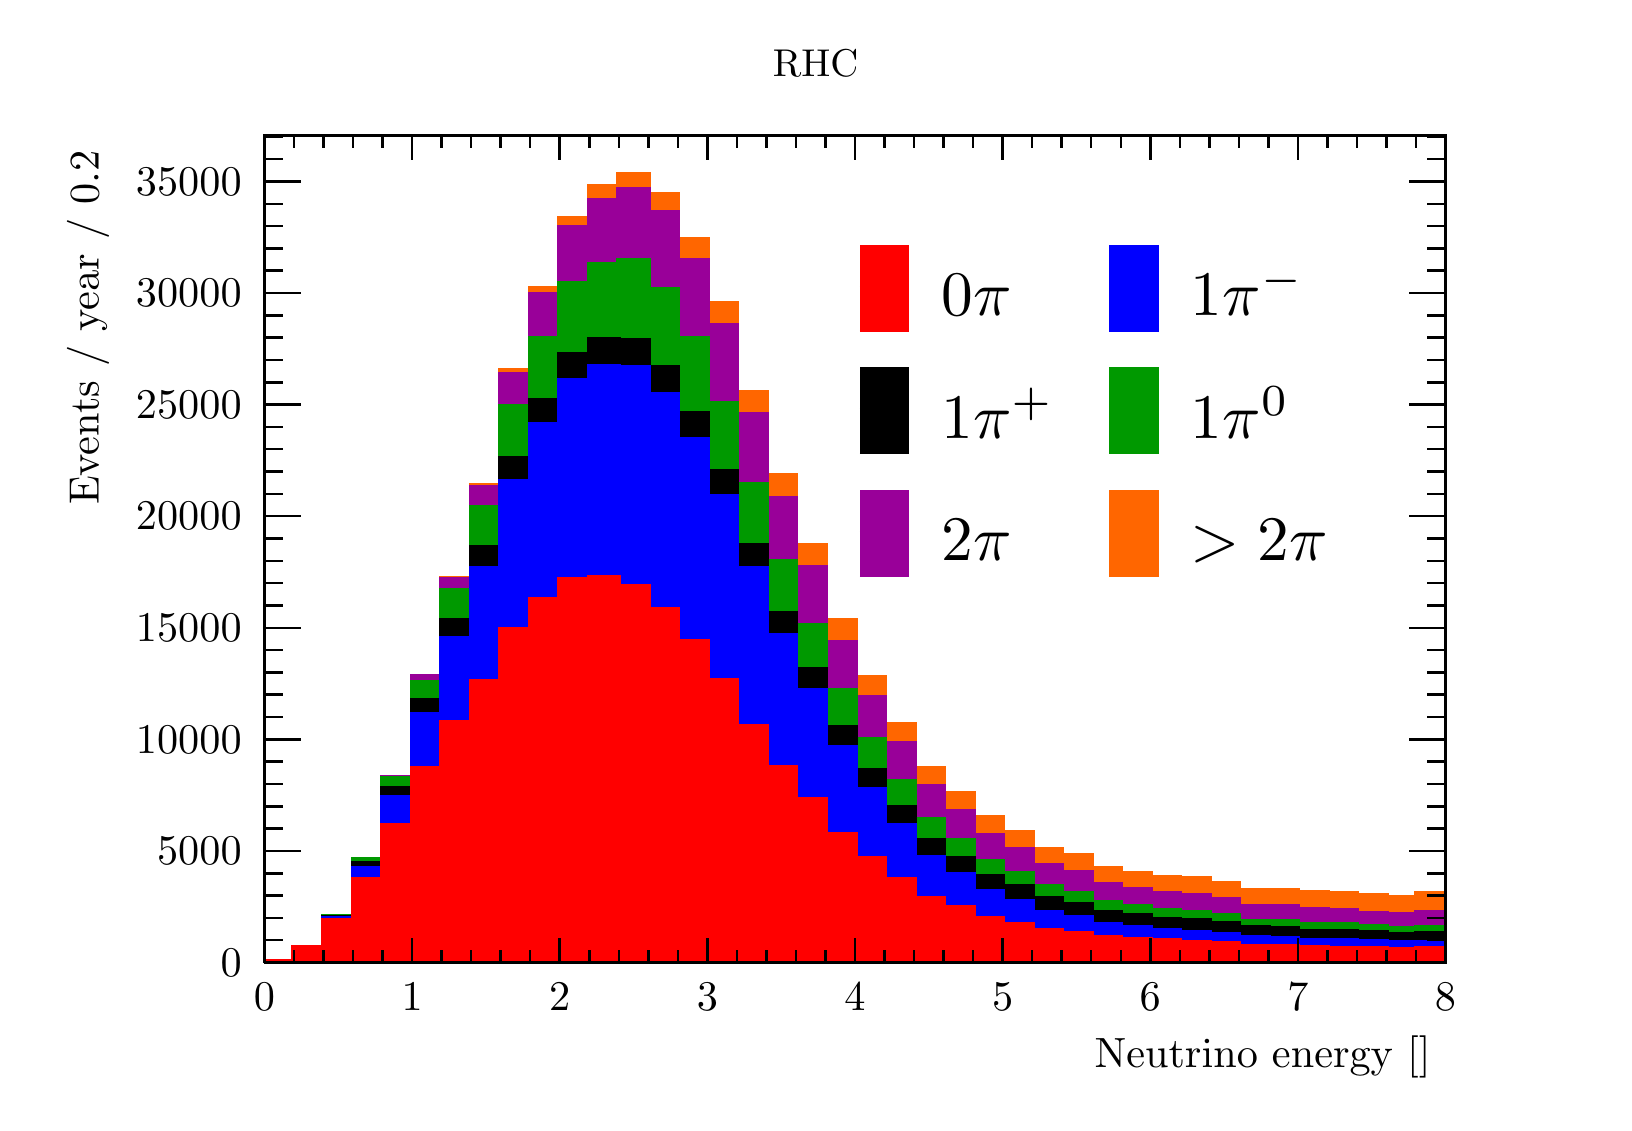
\begin{tikzpicture}
\pgfdeclareplotmark{cross} {
\pgfpathmoveto{\pgfpoint{-0.3\pgfplotmarksize}{\pgfplotmarksize}}
\pgfpathlineto{\pgfpoint{+0.3\pgfplotmarksize}{\pgfplotmarksize}}
\pgfpathlineto{\pgfpoint{+0.3\pgfplotmarksize}{0.3\pgfplotmarksize}}
\pgfpathlineto{\pgfpoint{+1\pgfplotmarksize}{0.3\pgfplotmarksize}}
\pgfpathlineto{\pgfpoint{+1\pgfplotmarksize}{-0.3\pgfplotmarksize}}
\pgfpathlineto{\pgfpoint{+0.3\pgfplotmarksize}{-0.3\pgfplotmarksize}}
\pgfpathlineto{\pgfpoint{+0.3\pgfplotmarksize}{-1.\pgfplotmarksize}}
\pgfpathlineto{\pgfpoint{-0.3\pgfplotmarksize}{-1.\pgfplotmarksize}}
\pgfpathlineto{\pgfpoint{-0.3\pgfplotmarksize}{-0.3\pgfplotmarksize}}
\pgfpathlineto{\pgfpoint{-1.\pgfplotmarksize}{-0.3\pgfplotmarksize}}
\pgfpathlineto{\pgfpoint{-1.\pgfplotmarksize}{0.3\pgfplotmarksize}}
\pgfpathlineto{\pgfpoint{-0.3\pgfplotmarksize}{0.3\pgfplotmarksize}}
\pgfpathclose
\pgfusepathqstroke
}
\pgfdeclareplotmark{cross*} {
\pgfpathmoveto{\pgfpoint{-0.3\pgfplotmarksize}{\pgfplotmarksize}}
\pgfpathlineto{\pgfpoint{+0.3\pgfplotmarksize}{\pgfplotmarksize}}
\pgfpathlineto{\pgfpoint{+0.3\pgfplotmarksize}{0.3\pgfplotmarksize}}
\pgfpathlineto{\pgfpoint{+1\pgfplotmarksize}{0.3\pgfplotmarksize}}
\pgfpathlineto{\pgfpoint{+1\pgfplotmarksize}{-0.3\pgfplotmarksize}}
\pgfpathlineto{\pgfpoint{+0.3\pgfplotmarksize}{-0.3\pgfplotmarksize}}
\pgfpathlineto{\pgfpoint{+0.3\pgfplotmarksize}{-1.\pgfplotmarksize}}
\pgfpathlineto{\pgfpoint{-0.3\pgfplotmarksize}{-1.\pgfplotmarksize}}
\pgfpathlineto{\pgfpoint{-0.3\pgfplotmarksize}{-0.3\pgfplotmarksize}}
\pgfpathlineto{\pgfpoint{-1.\pgfplotmarksize}{-0.3\pgfplotmarksize}}
\pgfpathlineto{\pgfpoint{-1.\pgfplotmarksize}{0.3\pgfplotmarksize}}
\pgfpathlineto{\pgfpoint{-0.3\pgfplotmarksize}{0.3\pgfplotmarksize}}
\pgfpathclose
\pgfusepathqfillstroke
}
\pgfdeclareplotmark{newstar} {
\pgfpathmoveto{\pgfqpoint{0pt}{\pgfplotmarksize}}
\pgfpathlineto{\pgfqpointpolar{44}{0.5\pgfplotmarksize}}
\pgfpathlineto{\pgfqpointpolar{18}{\pgfplotmarksize}}
\pgfpathlineto{\pgfqpointpolar{-20}{0.5\pgfplotmarksize}}
\pgfpathlineto{\pgfqpointpolar{-54}{\pgfplotmarksize}}
\pgfpathlineto{\pgfqpointpolar{-90}{0.5\pgfplotmarksize}}
\pgfpathlineto{\pgfqpointpolar{234}{\pgfplotmarksize}}
\pgfpathlineto{\pgfqpointpolar{198}{0.5\pgfplotmarksize}}
\pgfpathlineto{\pgfqpointpolar{162}{\pgfplotmarksize}}
\pgfpathlineto{\pgfqpointpolar{134}{0.5\pgfplotmarksize}}
\pgfpathclose
\pgfusepathqstroke
}
\pgfdeclareplotmark{newstar*} {
\pgfpathmoveto{\pgfqpoint{0pt}{\pgfplotmarksize}}
\pgfpathlineto{\pgfqpointpolar{44}{0.5\pgfplotmarksize}}
\pgfpathlineto{\pgfqpointpolar{18}{\pgfplotmarksize}}
\pgfpathlineto{\pgfqpointpolar{-20}{0.5\pgfplotmarksize}}
\pgfpathlineto{\pgfqpointpolar{-54}{\pgfplotmarksize}}
\pgfpathlineto{\pgfqpointpolar{-90}{0.5\pgfplotmarksize}}
\pgfpathlineto{\pgfqpointpolar{234}{\pgfplotmarksize}}
\pgfpathlineto{\pgfqpointpolar{198}{0.5\pgfplotmarksize}}
\pgfpathlineto{\pgfqpointpolar{162}{\pgfplotmarksize}}
\pgfpathlineto{\pgfqpointpolar{134}{0.5\pgfplotmarksize}}
\pgfpathclose
\pgfusepathqfillstroke
}
\definecolor{c}{rgb}{1,1,1};
\draw [color=c, fill=c] (0,0) rectangle (20,13.639);
\draw [color=c, fill=c] (3,1.77307) rectangle (18,12.2751);
\definecolor{c}{rgb}{0,0,0};
\draw [c,line width=0.9] (3,1.77307) -- (3,12.2751) -- (18,12.2751) -- (18,1.77307) -- (3,1.77307);
\definecolor{c}{rgb}{1,1,1};
\draw [color=c, fill=c] (3,1.77307) rectangle (18,12.2751);
\definecolor{c}{rgb}{0,0,0};
\draw [c,line width=0.9] (3,1.77307) -- (3,12.2751) -- (18,12.2751) -- (18,1.77307) -- (3,1.77307);
\draw [c,line width=0.9] (3,1.77307) -- (3.375,1.77307) -- (3.375,1.77307) -- (3.75,1.77307) -- (3.75,1.77307) -- (4.125,1.77307) -- (4.125,1.77307) -- (4.5,1.77307) -- (4.5,1.77307) -- (4.875,1.77307) -- (4.875,1.77307) -- (5.25,1.77307) --
 (5.25,1.77307) -- (5.625,1.77307) -- (5.625,1.77307) -- (6,1.77307) -- (6,1.77307) -- (6.375,1.77307) -- (6.375,1.77307) -- (6.75,1.77307) -- (6.75,1.77307) -- (7.125,1.77307) -- (7.125,1.77307) -- (7.5,1.77307) -- (7.5,1.77307) -- (7.875,1.77307)
 -- (7.875,1.77307) -- (8.25,1.77307) -- (8.25,1.77307) -- (8.625,1.77307) -- (8.625,1.77307) -- (9,1.77307) -- (9,1.77307) -- (9.375,1.77307) -- (9.375,1.77307) -- (9.75,1.77307) -- (9.75,1.77307) -- (10.125,1.77307) -- (10.125,1.77307) --
 (10.5,1.77307) -- (10.5,1.77307) -- (10.875,1.77307) -- (10.875,1.77307) -- (11.25,1.77307) -- (11.25,1.77307) -- (11.625,1.77307) -- (11.625,1.77307) -- (12,1.77307) -- (12,1.77307) -- (12.375,1.77307) -- (12.375,1.77307) -- (12.75,1.77307) --
 (12.75,1.77307) -- (13.125,1.77307) -- (13.125,1.77307) -- (13.5,1.77307) -- (13.5,1.77307) -- (13.875,1.77307) -- (13.875,1.77307) -- (14.25,1.77307) -- (14.25,1.77307) -- (14.625,1.77307) -- (14.625,1.77307) -- (15,1.77307) -- (15,1.77307) --
 (15.375,1.77307) -- (15.375,1.77307) -- (15.75,1.77307) -- (15.75,1.77307) -- (16.125,1.77307) -- (16.125,1.77307) -- (16.5,1.77307) -- (16.5,1.77307) -- (16.875,1.77307) -- (16.875,1.77307) -- (17.25,1.77307) -- (17.25,1.77307) -- (17.625,1.77307)
 -- (17.625,1.77307) -- (18,1.77307);
\draw [c,line width=0.9] (3,1.77307) -- (18,1.77307);
\draw [c,line width=0.9] (3,2.07994) -- (3,1.77307);
\draw [c,line width=0.9] (3.375,1.9265) -- (3.375,1.77307);
\draw [c,line width=0.9] (3.75,1.9265) -- (3.75,1.77307);
\draw [c,line width=0.9] (4.125,1.9265) -- (4.125,1.77307);
\draw [c,line width=0.9] (4.5,1.9265) -- (4.5,1.77307);
\draw [c,line width=0.9] (4.875,2.07994) -- (4.875,1.77307);
\draw [c,line width=0.9] (5.25,1.9265) -- (5.25,1.77307);
\draw [c,line width=0.9] (5.625,1.9265) -- (5.625,1.77307);
\draw [c,line width=0.9] (6,1.9265) -- (6,1.77307);
\draw [c,line width=0.9] (6.375,1.9265) -- (6.375,1.77307);
\draw [c,line width=0.9] (6.75,2.07994) -- (6.75,1.77307);
\draw [c,line width=0.9] (7.125,1.9265) -- (7.125,1.77307);
\draw [c,line width=0.9] (7.5,1.9265) -- (7.5,1.77307);
\draw [c,line width=0.9] (7.875,1.9265) -- (7.875,1.77307);
\draw [c,line width=0.9] (8.25,1.9265) -- (8.25,1.77307);
\draw [c,line width=0.9] (8.625,2.07994) -- (8.625,1.77307);
\draw [c,line width=0.9] (9,1.9265) -- (9,1.77307);
\draw [c,line width=0.9] (9.375,1.9265) -- (9.375,1.77307);
\draw [c,line width=0.9] (9.75,1.9265) -- (9.75,1.77307);
\draw [c,line width=0.9] (10.125,1.9265) -- (10.125,1.77307);
\draw [c,line width=0.9] (10.5,2.07994) -- (10.5,1.77307);
\draw [c,line width=0.9] (10.875,1.9265) -- (10.875,1.77307);
\draw [c,line width=0.9] (11.25,1.9265) -- (11.25,1.77307);
\draw [c,line width=0.9] (11.625,1.9265) -- (11.625,1.77307);
\draw [c,line width=0.9] (12,1.9265) -- (12,1.77307);
\draw [c,line width=0.9] (12.375,2.07994) -- (12.375,1.77307);
\draw [c,line width=0.9] (12.75,1.9265) -- (12.75,1.77307);
\draw [c,line width=0.9] (13.125,1.9265) -- (13.125,1.77307);
\draw [c,line width=0.9] (13.5,1.9265) -- (13.5,1.77307);
\draw [c,line width=0.9] (13.875,1.9265) -- (13.875,1.77307);
\draw [c,line width=0.9] (14.25,2.07994) -- (14.25,1.77307);
\draw [c,line width=0.9] (14.625,1.9265) -- (14.625,1.77307);
\draw [c,line width=0.9] (15,1.9265) -- (15,1.77307);
\draw [c,line width=0.9] (15.375,1.9265) -- (15.375,1.77307);
\draw [c,line width=0.9] (15.75,1.9265) -- (15.75,1.77307);
\draw [c,line width=0.9] (16.125,2.07994) -- (16.125,1.77307);
\draw [c,line width=0.9] (16.5,1.9265) -- (16.5,1.77307);
\draw [c,line width=0.9] (16.875,1.9265) -- (16.875,1.77307);
\draw [c,line width=0.9] (17.25,1.9265) -- (17.25,1.77307);
\draw [c,line width=0.9] (17.625,1.9265) -- (17.625,1.77307);
\draw [c,line width=0.9] (18,2.07994) -- (18,1.77307);
\draw [anchor=base] (3,1.15931) node[scale=1.52731, color=c, rotate=0]{0};
\draw [anchor=base] (4.875,1.15931) node[scale=1.52731, color=c, rotate=0]{1};
\draw [anchor=base] (6.75,1.15931) node[scale=1.52731, color=c, rotate=0]{2};
\draw [anchor=base] (8.625,1.15931) node[scale=1.52731, color=c, rotate=0]{3};
\draw [anchor=base] (10.5,1.15931) node[scale=1.52731, color=c, rotate=0]{4};
\draw [anchor=base] (12.375,1.15931) node[scale=1.52731, color=c, rotate=0]{5};
\draw [anchor=base] (14.25,1.15931) node[scale=1.52731, color=c, rotate=0]{6};
\draw [anchor=base] (16.125,1.15931) node[scale=1.52731, color=c, rotate=0]{7};
\draw [anchor=base] (18,1.15931) node[scale=1.52731, color=c, rotate=0]{8};
\draw [anchor= east] (18,0.572837) node[scale=1.52731, color=c, rotate=0]{ Neutrino energy [\si{\giga\electronvolt}] };
\draw [c,line width=0.9] (3,12.2751) -- (18,12.2751);
\draw [c,line width=0.9] (3,11.9682) -- (3,12.2751);
\draw [c,line width=0.9] (3.375,12.1216) -- (3.375,12.2751);
\draw [c,line width=0.9] (3.75,12.1216) -- (3.75,12.2751);
\draw [c,line width=0.9] (4.125,12.1216) -- (4.125,12.2751);
\draw [c,line width=0.9] (4.5,12.1216) -- (4.5,12.2751);
\draw [c,line width=0.9] (4.875,11.9682) -- (4.875,12.2751);
\draw [c,line width=0.9] (5.25,12.1216) -- (5.25,12.2751);
\draw [c,line width=0.9] (5.625,12.1216) -- (5.625,12.2751);
\draw [c,line width=0.9] (6,12.1216) -- (6,12.2751);
\draw [c,line width=0.9] (6.375,12.1216) -- (6.375,12.2751);
\draw [c,line width=0.9] (6.75,11.9682) -- (6.75,12.2751);
\draw [c,line width=0.9] (7.125,12.1216) -- (7.125,12.2751);
\draw [c,line width=0.9] (7.5,12.1216) -- (7.5,12.2751);
\draw [c,line width=0.9] (7.875,12.1216) -- (7.875,12.2751);
\draw [c,line width=0.9] (8.25,12.1216) -- (8.25,12.2751);
\draw [c,line width=0.9] (8.625,11.9682) -- (8.625,12.2751);
\draw [c,line width=0.9] (9,12.1216) -- (9,12.2751);
\draw [c,line width=0.9] (9.375,12.1216) -- (9.375,12.2751);
\draw [c,line width=0.9] (9.75,12.1216) -- (9.75,12.2751);
\draw [c,line width=0.9] (10.125,12.1216) -- (10.125,12.2751);
\draw [c,line width=0.9] (10.5,11.9682) -- (10.5,12.2751);
\draw [c,line width=0.9] (10.875,12.1216) -- (10.875,12.2751);
\draw [c,line width=0.9] (11.25,12.1216) -- (11.25,12.2751);
\draw [c,line width=0.9] (11.625,12.1216) -- (11.625,12.2751);
\draw [c,line width=0.9] (12,12.1216) -- (12,12.2751);
\draw [c,line width=0.9] (12.375,11.9682) -- (12.375,12.2751);
\draw [c,line width=0.9] (12.75,12.1216) -- (12.75,12.2751);
\draw [c,line width=0.9] (13.125,12.1216) -- (13.125,12.2751);
\draw [c,line width=0.9] (13.5,12.1216) -- (13.5,12.2751);
\draw [c,line width=0.9] (13.875,12.1216) -- (13.875,12.2751);
\draw [c,line width=0.9] (14.25,11.9682) -- (14.25,12.2751);
\draw [c,line width=0.9] (14.625,12.1216) -- (14.625,12.2751);
\draw [c,line width=0.9] (15,12.1216) -- (15,12.2751);
\draw [c,line width=0.9] (15.375,12.1216) -- (15.375,12.2751);
\draw [c,line width=0.9] (15.75,12.1216) -- (15.75,12.2751);
\draw [c,line width=0.9] (16.125,11.9682) -- (16.125,12.2751);
\draw [c,line width=0.9] (16.5,12.1216) -- (16.5,12.2751);
\draw [c,line width=0.9] (16.875,12.1216) -- (16.875,12.2751);
\draw [c,line width=0.9] (17.25,12.1216) -- (17.25,12.2751);
\draw [c,line width=0.9] (17.625,12.1216) -- (17.625,12.2751);
\draw [c,line width=0.9] (18,11.9682) -- (18,12.2751);
\draw [c,line width=0.9] (3,1.77307) -- (3,12.2751);
\draw [c,line width=0.9] (3.462,1.77307) -- (3,1.77307);
\draw [c,line width=0.9] (3.231,2.05649) -- (3,2.05649);
\draw [c,line width=0.9] (3.231,2.33992) -- (3,2.33992);
\draw [c,line width=0.9] (3.231,2.62335) -- (3,2.62335);
\draw [c,line width=0.9] (3.231,2.90677) -- (3,2.90677);
\draw [c,line width=0.9] (3.462,3.1902) -- (3,3.1902);
\draw [c,line width=0.9] (3.231,3.47362) -- (3,3.47362);
\draw [c,line width=0.9] (3.231,3.75705) -- (3,3.75705);
\draw [c,line width=0.9] (3.231,4.04048) -- (3,4.04048);
\draw [c,line width=0.9] (3.231,4.3239) -- (3,4.3239);
\draw [c,line width=0.9] (3.462,4.60733) -- (3,4.60733);
\draw [c,line width=0.9] (3.231,4.89076) -- (3,4.89076);
\draw [c,line width=0.9] (3.231,5.17418) -- (3,5.17418);
\draw [c,line width=0.9] (3.231,5.45761) -- (3,5.45761);
\draw [c,line width=0.9] (3.231,5.74104) -- (3,5.74104);
\draw [c,line width=0.9] (3.462,6.02446) -- (3,6.02446);
\draw [c,line width=0.9] (3.231,6.30789) -- (3,6.30789);
\draw [c,line width=0.9] (3.231,6.59131) -- (3,6.59131);
\draw [c,line width=0.9] (3.231,6.87474) -- (3,6.87474);
\draw [c,line width=0.9] (3.231,7.15817) -- (3,7.15817);
\draw [c,line width=0.9] (3.462,7.44159) -- (3,7.44159);
\draw [c,line width=0.9] (3.231,7.72502) -- (3,7.72502);
\draw [c,line width=0.9] (3.231,8.00845) -- (3,8.00845);
\draw [c,line width=0.9] (3.231,8.29187) -- (3,8.29187);
\draw [c,line width=0.9] (3.231,8.5753) -- (3,8.5753);
\draw [c,line width=0.9] (3.462,8.85873) -- (3,8.85873);
\draw [c,line width=0.9] (3.231,9.14215) -- (3,9.14215);
\draw [c,line width=0.9] (3.231,9.42558) -- (3,9.42558);
\draw [c,line width=0.9] (3.231,9.70901) -- (3,9.70901);
\draw [c,line width=0.9] (3.231,9.99243) -- (3,9.99243);
\draw [c,line width=0.9] (3.462,10.2759) -- (3,10.2759);
\draw [c,line width=0.9] (3.231,10.5593) -- (3,10.5593);
\draw [c,line width=0.9] (3.231,10.8427) -- (3,10.8427);
\draw [c,line width=0.9] (3.231,11.1261) -- (3,11.1261);
\draw [c,line width=0.9] (3.231,11.4096) -- (3,11.4096);
\draw [c,line width=0.9] (3.462,11.693) -- (3,11.693);
\draw [c,line width=0.9] (3.462,11.693) -- (3,11.693);
\draw [c,line width=0.9] (3.231,11.9764) -- (3,11.9764);
\draw [c,line width=0.9] (3.231,12.2598) -- (3,12.2598);
\draw [anchor= east] (2.9,1.77307) node[scale=1.52731, color=c, rotate=0]{0};
\draw [anchor= east] (2.9,3.1902) node[scale=1.52731, color=c, rotate=0]{5000};
\draw [anchor= east] (2.9,4.60733) node[scale=1.52731, color=c, rotate=0]{10000};
\draw [anchor= east] (2.9,6.02446) node[scale=1.52731, color=c, rotate=0]{15000};
\draw [anchor= east] (2.9,7.44159) node[scale=1.52731, color=c, rotate=0]{20000};
\draw [anchor= east] (2.9,8.85873) node[scale=1.52731, color=c, rotate=0]{25000};
\draw [anchor= east] (2.9,10.2759) node[scale=1.52731, color=c, rotate=0]{30000};
\draw [anchor= east] (2.9,11.693) node[scale=1.52731, color=c, rotate=0]{35000};
\draw [anchor= east] (0.76,12.2751) node[scale=1.52731, color=c, rotate=90]{ Events / year / \SI{0.2}{\giga\electronvolt} };
\draw [c,line width=0.9] (18,1.77307) -- (18,12.2751);
\draw [c,line width=0.9] (17.538,1.77307) -- (18,1.77307);
\draw [c,line width=0.9] (17.769,2.05649) -- (18,2.05649);
\draw [c,line width=0.9] (17.769,2.33992) -- (18,2.33992);
\draw [c,line width=0.9] (17.769,2.62335) -- (18,2.62335);
\draw [c,line width=0.9] (17.769,2.90677) -- (18,2.90677);
\draw [c,line width=0.9] (17.538,3.1902) -- (18,3.1902);
\draw [c,line width=0.9] (17.769,3.47362) -- (18,3.47362);
\draw [c,line width=0.9] (17.769,3.75705) -- (18,3.75705);
\draw [c,line width=0.9] (17.769,4.04048) -- (18,4.04048);
\draw [c,line width=0.9] (17.769,4.3239) -- (18,4.3239);
\draw [c,line width=0.9] (17.538,4.60733) -- (18,4.60733);
\draw [c,line width=0.9] (17.769,4.89076) -- (18,4.89076);
\draw [c,line width=0.9] (17.769,5.17418) -- (18,5.17418);
\draw [c,line width=0.9] (17.769,5.45761) -- (18,5.45761);
\draw [c,line width=0.9] (17.769,5.74104) -- (18,5.74104);
\draw [c,line width=0.9] (17.538,6.02446) -- (18,6.02446);
\draw [c,line width=0.9] (17.769,6.30789) -- (18,6.30789);
\draw [c,line width=0.9] (17.769,6.59131) -- (18,6.59131);
\draw [c,line width=0.9] (17.769,6.87474) -- (18,6.87474);
\draw [c,line width=0.9] (17.769,7.15817) -- (18,7.15817);
\draw [c,line width=0.9] (17.538,7.44159) -- (18,7.44159);
\draw [c,line width=0.9] (17.769,7.72502) -- (18,7.72502);
\draw [c,line width=0.9] (17.769,8.00845) -- (18,8.00845);
\draw [c,line width=0.9] (17.769,8.29187) -- (18,8.29187);
\draw [c,line width=0.9] (17.769,8.5753) -- (18,8.5753);
\draw [c,line width=0.9] (17.538,8.85873) -- (18,8.85873);
\draw [c,line width=0.9] (17.769,9.14215) -- (18,9.14215);
\draw [c,line width=0.9] (17.769,9.42558) -- (18,9.42558);
\draw [c,line width=0.9] (17.769,9.70901) -- (18,9.70901);
\draw [c,line width=0.9] (17.769,9.99243) -- (18,9.99243);
\draw [c,line width=0.9] (17.538,10.2759) -- (18,10.2759);
\draw [c,line width=0.9] (17.769,10.5593) -- (18,10.5593);
\draw [c,line width=0.9] (17.769,10.8427) -- (18,10.8427);
\draw [c,line width=0.9] (17.769,11.1261) -- (18,11.1261);
\draw [c,line width=0.9] (17.769,11.4096) -- (18,11.4096);
\draw [c,line width=0.9] (17.538,11.693) -- (18,11.693);
\draw [c,line width=0.9] (17.538,11.693) -- (18,11.693);
\draw [c,line width=0.9] (17.769,11.9764) -- (18,11.9764);
\draw [c,line width=0.9] (17.769,12.2598) -- (18,12.2598);
\definecolor{c}{rgb}{1,0.4,0};
\draw [c, fill=c] (3,1.77307) -- (3,1.7815) -- (3.375,1.7815) -- (3.375,1.96202) -- (3.75,1.96202) -- (3.75,2.35282) -- (4.125,2.35282) -- (4.125,3.08114) -- (4.5,3.08114) -- (4.5,4.12375) -- (4.875,4.12375) -- (4.875,5.40336) -- (5.25,5.40336) --
 (5.25,6.64876) -- (5.625,6.64876) -- (5.625,7.8288) -- (6,7.8288) -- (6,9.28607) -- (6.375,9.28607) -- (6.375,10.3376) -- (6.75,10.3376) -- (6.75,11.221) -- (7.125,11.221) -- (7.125,11.624) -- (7.5,11.624) -- (7.5,11.775) -- (7.875,11.775) --
 (7.875,11.5305) -- (8.25,11.5305) -- (8.25,10.9544) -- (8.625,10.9544) -- (8.625,10.138) -- (9,10.138) -- (9,9.01345) -- (9.375,9.01345) -- (9.375,7.95684) -- (9.75,7.95684) -- (9.75,7.06708) -- (10.125,7.06708) -- (10.125,6.11084) -- (10.5,6.11084)
 -- (10.5,5.39843) -- (10.875,5.39843) -- (10.875,4.79926) -- (11.25,4.79926) -- (11.25,4.23827) -- (11.625,4.23827) -- (11.625,3.92255) -- (12,3.92255) -- (12,3.60921) -- (12.375,3.60921) -- (12.375,3.42486) -- (12.75,3.42486) -- (12.75,3.21332) --
 (13.125,3.21332) -- (13.125,3.13697) -- (13.5,3.13697) -- (13.5,2.9636) -- (13.875,2.9636) -- (13.875,2.90061) -- (14.25,2.90061) -- (14.25,2.85655) -- (14.625,2.85655) -- (14.625,2.83572) -- (15,2.83572) -- (15,2.78053) -- (15.375,2.78053) --
 (15.375,2.69352) -- (15.75,2.69352) -- (15.75,2.6905) -- (16.125,2.6905) -- (16.125,2.65885) -- (16.5,2.65885) -- (16.5,2.64612) -- (16.875,2.64612) -- (16.875,2.62799) -- (17.25,2.62799) -- (17.25,2.59379) -- (17.625,2.59379) -- (17.625,2.65169) --
 (18,2.65169) -- (18,1.77307);
\draw [c,line width=1.8] (3,1.7815) -- (3.375,1.7815) -- (3.375,1.96202) -- (3.75,1.96202) -- (3.75,2.35282) -- (4.125,2.35282) -- (4.125,3.08114) -- (4.5,3.08114) -- (4.5,4.12375) -- (4.875,4.12375) -- (4.875,5.40336) -- (5.25,5.40336) --
 (5.25,6.64876) -- (5.625,6.64876) -- (5.625,7.8288) -- (6,7.8288) -- (6,9.28607) -- (6.375,9.28607) -- (6.375,10.3376) -- (6.75,10.3376) -- (6.75,11.221) -- (7.125,11.221) -- (7.125,11.624) -- (7.5,11.624) -- (7.5,11.775) -- (7.875,11.775) --
 (7.875,11.5305) -- (8.25,11.5305) -- (8.25,10.9544) -- (8.625,10.9544) -- (8.625,10.138) -- (9,10.138) -- (9,9.01345) -- (9.375,9.01345) -- (9.375,7.95684) -- (9.75,7.95684) -- (9.75,7.06708) -- (10.125,7.06708) -- (10.125,6.11084) -- (10.5,6.11084)
 -- (10.5,5.39843) -- (10.875,5.39843) -- (10.875,4.79926) -- (11.25,4.79926) -- (11.25,4.23827) -- (11.625,4.23827) -- (11.625,3.92255) -- (12,3.92255) -- (12,3.60921) -- (12.375,3.60921) -- (12.375,3.42486) -- (12.75,3.42486) -- (12.75,3.21332) --
 (13.125,3.21332) -- (13.125,3.13697) -- (13.5,3.13697) -- (13.5,2.9636) -- (13.875,2.9636) -- (13.875,2.90061) -- (14.25,2.90061) -- (14.25,2.85655) -- (14.625,2.85655) -- (14.625,2.83572) -- (15,2.83572) -- (15,2.78053) -- (15.375,2.78053) --
 (15.375,2.69352) -- (15.75,2.69352) -- (15.75,2.6905) -- (16.125,2.6905) -- (16.125,2.65885) -- (16.5,2.65885) -- (16.5,2.64612) -- (16.875,2.64612) -- (16.875,2.62799) -- (17.25,2.62799) -- (17.25,2.59379) -- (17.625,2.59379) -- (17.625,2.65169) --
 (18,2.65169);
\definecolor{c}{rgb}{0.999,0.999,0.999};
\draw [c, fill=c] (3,1.77307) -- (3,1.7815) -- (3.375,1.7815) -- (3.375,1.96202) -- (3.75,1.96202) -- (3.75,2.35282) -- (4.125,2.35282) -- (4.125,3.08114) -- (4.5,3.08114) -- (4.5,4.12328) -- (4.875,4.12328) -- (4.875,5.40049) -- (5.25,5.40049) --
 (5.25,6.64002) -- (5.625,6.64002) -- (5.625,7.80478) -- (6,7.80478) -- (6,9.23851) -- (6.375,9.23851) -- (6.375,10.2601) -- (6.75,10.2601) -- (6.75,11.1093) -- (7.125,11.1093) -- (7.125,11.4558) -- (7.5,11.4558) -- (7.5,11.5846) -- (7.875,11.5846)
 -- (7.875,11.2953) -- (8.25,11.2953) -- (8.25,10.6901) -- (8.625,10.6901) -- (8.625,9.85899) -- (9,9.85899) -- (9,8.72858) -- (9.375,8.72858) -- (9.375,7.66768) -- (9.75,7.66768) -- (9.75,6.78873) -- (10.125,6.78873) -- (10.125,5.83965) --
 (10.5,5.83965) -- (10.5,5.14298) -- (10.875,5.14298) -- (10.875,4.55511) -- (11.25,4.55511) -- (11.25,4.00764) -- (11.625,4.00764) -- (11.625,3.69223) -- (12,3.69223) -- (12,3.39305) -- (12.375,3.39305) -- (12.375,3.20918) -- (12.75,3.20918) --
 (12.75,3.01036) -- (13.125,3.01036) -- (13.125,2.91525) -- (13.5,2.91525) -- (13.5,2.7608) -- (13.875,2.7608) -- (13.875,2.7045) -- (14.25,2.7045) -- (14.25,2.64501) -- (14.625,2.64501) -- (14.625,2.61924) -- (15,2.61924) -- (15,2.56819) --
 (15.375,2.56819) -- (15.375,2.48611) -- (15.75,2.48611) -- (15.75,2.4823) -- (16.125,2.4823) -- (16.125,2.44317) -- (16.5,2.44317) -- (16.5,2.43426) -- (16.875,2.43426) -- (16.875,2.39863) -- (17.25,2.39863) -- (17.25,2.37907) -- (17.625,2.37907) --
 (17.625,2.40929) -- (18,2.40929) -- (18,1.77307);
\definecolor{c}{rgb}{0.6,0,0.6};
\draw [c,line width=1.8] (3,1.7815) -- (3.375,1.7815) -- (3.375,1.96202) -- (3.75,1.96202) -- (3.75,2.35282) -- (4.125,2.35282) -- (4.125,3.08114) -- (4.5,3.08114) -- (4.5,4.12328) -- (4.875,4.12328) -- (4.875,5.40049) -- (5.25,5.40049) --
 (5.25,6.64002) -- (5.625,6.64002) -- (5.625,7.80478) -- (6,7.80478) -- (6,9.23851) -- (6.375,9.23851) -- (6.375,10.2601) -- (6.75,10.2601) -- (6.75,11.1093) -- (7.125,11.1093) -- (7.125,11.4558) -- (7.5,11.4558) -- (7.5,11.5846) -- (7.875,11.5846)
 -- (7.875,11.2953) -- (8.25,11.2953) -- (8.25,10.6901) -- (8.625,10.6901) -- (8.625,9.85899) -- (9,9.85899) -- (9,8.72858) -- (9.375,8.72858) -- (9.375,7.66768) -- (9.75,7.66768) -- (9.75,6.78873) -- (10.125,6.78873) -- (10.125,5.83965) --
 (10.5,5.83965) -- (10.5,5.14298) -- (10.875,5.14298) -- (10.875,4.55511) -- (11.25,4.55511) -- (11.25,4.00764) -- (11.625,4.00764) -- (11.625,3.69223) -- (12,3.69223) -- (12,3.39305) -- (12.375,3.39305) -- (12.375,3.20918) -- (12.75,3.20918) --
 (12.75,3.01036) -- (13.125,3.01036) -- (13.125,2.91525) -- (13.5,2.91525) -- (13.5,2.7608) -- (13.875,2.7608) -- (13.875,2.7045) -- (14.25,2.7045) -- (14.25,2.64501) -- (14.625,2.64501) -- (14.625,2.61924) -- (15,2.61924) -- (15,2.56819) --
 (15.375,2.56819) -- (15.375,2.48611) -- (15.75,2.48611) -- (15.75,2.4823) -- (16.125,2.4823) -- (16.125,2.44317) -- (16.5,2.44317) -- (16.5,2.43426) -- (16.875,2.43426) -- (16.875,2.39863) -- (17.25,2.39863) -- (17.25,2.37907) -- (17.625,2.37907) --
 (17.625,2.40929) -- (18,2.40929);
\draw [c,line width=1.8] (3,1.7815) -- (3.375,1.7815) -- (3.375,1.96202) -- (3.75,1.96202) -- (3.75,2.35282) -- (4.125,2.35282) -- (4.125,3.08114) -- (4.5,3.08114) -- (4.5,4.12328) -- (4.875,4.12328) -- (4.875,5.40049) -- (5.25,5.40049) --
 (5.25,6.64002) -- (5.625,6.64002) -- (5.625,7.80478) -- (6,7.80478) -- (6,9.23851) -- (6.375,9.23851) -- (6.375,10.2601) -- (6.75,10.2601) -- (6.75,11.1093) -- (7.125,11.1093) -- (7.125,11.4558) -- (7.5,11.4558) -- (7.5,11.5846) -- (7.875,11.5846)
 -- (7.875,11.2953) -- (8.25,11.2953) -- (8.25,10.6901) -- (8.625,10.6901) -- (8.625,9.85899) -- (9,9.85899) -- (9,8.72858) -- (9.375,8.72858) -- (9.375,7.66768) -- (9.75,7.66768) -- (9.75,6.78873) -- (10.125,6.78873) -- (10.125,5.83965) --
 (10.5,5.83965) -- (10.5,5.14298) -- (10.875,5.14298) -- (10.875,4.55511) -- (11.25,4.55511) -- (11.25,4.00764) -- (11.625,4.00764) -- (11.625,3.69223) -- (12,3.69223) -- (12,3.39305) -- (12.375,3.39305) -- (12.375,3.20918) -- (12.75,3.20918) --
 (12.75,3.01036) -- (13.125,3.01036) -- (13.125,2.91525) -- (13.5,2.91525) -- (13.5,2.7608) -- (13.875,2.7608) -- (13.875,2.7045) -- (14.25,2.7045) -- (14.25,2.64501) -- (14.625,2.64501) -- (14.625,2.61924) -- (15,2.61924) -- (15,2.56819) --
 (15.375,2.56819) -- (15.375,2.48611) -- (15.75,2.48611) -- (15.75,2.4823) -- (16.125,2.4823) -- (16.125,2.44317) -- (16.5,2.44317) -- (16.5,2.43426) -- (16.875,2.43426) -- (16.875,2.39863) -- (17.25,2.39863) -- (17.25,2.37907) -- (17.625,2.37907) --
 (17.625,2.40929) -- (18,2.40929);
\draw [c, fill=c] (3,1.77307) -- (3,1.7815) -- (3.375,1.7815) -- (3.375,1.96202) -- (3.75,1.96202) -- (3.75,2.35282) -- (4.125,2.35282) -- (4.125,3.08114) -- (4.5,3.08114) -- (4.5,4.12328) -- (4.875,4.12328) -- (4.875,5.40049) -- (5.25,5.40049) --
 (5.25,6.64002) -- (5.625,6.64002) -- (5.625,7.80478) -- (6,7.80478) -- (6,9.23851) -- (6.375,9.23851) -- (6.375,10.2601) -- (6.75,10.2601) -- (6.75,11.1093) -- (7.125,11.1093) -- (7.125,11.4558) -- (7.5,11.4558) -- (7.5,11.5846) -- (7.875,11.5846)
 -- (7.875,11.2953) -- (8.25,11.2953) -- (8.25,10.6901) -- (8.625,10.6901) -- (8.625,9.85899) -- (9,9.85899) -- (9,8.72858) -- (9.375,8.72858) -- (9.375,7.66768) -- (9.75,7.66768) -- (9.75,6.78873) -- (10.125,6.78873) -- (10.125,5.83965) --
 (10.5,5.83965) -- (10.5,5.14298) -- (10.875,5.14298) -- (10.875,4.55511) -- (11.25,4.55511) -- (11.25,4.00764) -- (11.625,4.00764) -- (11.625,3.69223) -- (12,3.69223) -- (12,3.39305) -- (12.375,3.39305) -- (12.375,3.20918) -- (12.75,3.20918) --
 (12.75,3.01036) -- (13.125,3.01036) -- (13.125,2.91525) -- (13.5,2.91525) -- (13.5,2.7608) -- (13.875,2.7608) -- (13.875,2.7045) -- (14.25,2.7045) -- (14.25,2.64501) -- (14.625,2.64501) -- (14.625,2.61924) -- (15,2.61924) -- (15,2.56819) --
 (15.375,2.56819) -- (15.375,2.48611) -- (15.75,2.48611) -- (15.75,2.4823) -- (16.125,2.4823) -- (16.125,2.44317) -- (16.5,2.44317) -- (16.5,2.43426) -- (16.875,2.43426) -- (16.875,2.39863) -- (17.25,2.39863) -- (17.25,2.37907) -- (17.625,2.37907) --
 (17.625,2.40929) -- (18,2.40929) -- (18,1.77307);
\draw [c,line width=1.8] (3,1.7815) -- (3.375,1.7815) -- (3.375,1.96202) -- (3.75,1.96202) -- (3.75,2.35282) -- (4.125,2.35282) -- (4.125,3.08114) -- (4.5,3.08114) -- (4.5,4.12328) -- (4.875,4.12328) -- (4.875,5.40049) -- (5.25,5.40049) --
 (5.25,6.64002) -- (5.625,6.64002) -- (5.625,7.80478) -- (6,7.80478) -- (6,9.23851) -- (6.375,9.23851) -- (6.375,10.2601) -- (6.75,10.2601) -- (6.75,11.1093) -- (7.125,11.1093) -- (7.125,11.4558) -- (7.5,11.4558) -- (7.5,11.5846) -- (7.875,11.5846)
 -- (7.875,11.2953) -- (8.25,11.2953) -- (8.25,10.6901) -- (8.625,10.6901) -- (8.625,9.85899) -- (9,9.85899) -- (9,8.72858) -- (9.375,8.72858) -- (9.375,7.66768) -- (9.75,7.66768) -- (9.75,6.78873) -- (10.125,6.78873) -- (10.125,5.83965) --
 (10.5,5.83965) -- (10.5,5.14298) -- (10.875,5.14298) -- (10.875,4.55511) -- (11.25,4.55511) -- (11.25,4.00764) -- (11.625,4.00764) -- (11.625,3.69223) -- (12,3.69223) -- (12,3.39305) -- (12.375,3.39305) -- (12.375,3.20918) -- (12.75,3.20918) --
 (12.75,3.01036) -- (13.125,3.01036) -- (13.125,2.91525) -- (13.5,2.91525) -- (13.5,2.7608) -- (13.875,2.7608) -- (13.875,2.7045) -- (14.25,2.7045) -- (14.25,2.64501) -- (14.625,2.64501) -- (14.625,2.61924) -- (15,2.61924) -- (15,2.56819) --
 (15.375,2.56819) -- (15.375,2.48611) -- (15.75,2.48611) -- (15.75,2.4823) -- (16.125,2.4823) -- (16.125,2.44317) -- (16.5,2.44317) -- (16.5,2.43426) -- (16.875,2.43426) -- (16.875,2.39863) -- (17.25,2.39863) -- (17.25,2.37907) -- (17.625,2.37907) --
 (17.625,2.40929) -- (18,2.40929);
\definecolor{c}{rgb}{0.999,0.999,0.999};
\draw [c, fill=c] (3,1.77307) -- (3,1.7815) -- (3.375,1.7815) -- (3.375,1.96202) -- (3.75,1.96202) -- (3.75,2.35267) -- (4.125,2.35267) -- (4.125,3.07923) -- (4.5,3.07923) -- (4.5,4.10848) -- (4.875,4.10848) -- (4.875,5.33592) -- (5.25,5.33592) --
 (5.25,6.49559) -- (5.625,6.49559) -- (5.625,7.54934) -- (6,7.54934) -- (6,8.83308) -- (6.375,8.83308) -- (6.375,9.70025) -- (6.75,9.70025) -- (6.75,10.4023) -- (7.125,10.4023) -- (7.125,10.6382) -- (7.5,10.6382) -- (7.5,10.6848) -- (7.875,10.6848)
 -- (7.875,10.3242) -- (8.25,10.3242) -- (8.25,9.7028) -- (8.625,9.7028) -- (8.625,8.86696) -- (9,8.86696) -- (9,7.84646) -- (9.375,7.84646) -- (9.375,6.86413) -- (9.75,6.86413) -- (9.75,6.05215) -- (10.125,6.05215) -- (10.125,5.22919) --
 (10.5,5.22919) -- (10.5,4.60235) -- (10.875,4.60235) -- (10.875,4.07333) -- (11.25,4.07333) -- (11.25,3.59266) -- (11.625,3.59266) -- (11.625,3.3202) -- (12,3.3202) -- (12,3.05299) -- (12.375,3.05299) -- (12.375,2.90014) -- (12.75,2.90014) --
 (12.75,2.74315) -- (13.125,2.74315) -- (13.125,2.65551) -- (13.5,2.65551) -- (13.5,2.53097) -- (13.875,2.53097) -- (13.875,2.4823) -- (14.25,2.4823) -- (14.25,2.42997) -- (14.625,2.42997) -- (14.625,2.41024) -- (15,2.41024) -- (15,2.36491) --
 (15.375,2.36491) -- (15.375,2.29652) -- (15.75,2.29652) -- (15.75,2.29143) -- (16.125,2.29143) -- (16.125,2.26184) -- (16.5,2.26184) -- (16.5,2.25564) -- (16.875,2.25564) -- (16.875,2.22526) -- (17.25,2.22526) -- (17.25,2.21015) -- (17.625,2.21015)
 -- (17.625,2.22113) -- (18,2.22113) -- (18,1.77307);
\definecolor{c}{rgb}{0,0.6,0};
\draw [c,line width=1.8] (3,1.7815) -- (3.375,1.7815) -- (3.375,1.96202) -- (3.75,1.96202) -- (3.75,2.35267) -- (4.125,2.35267) -- (4.125,3.07923) -- (4.5,3.07923) -- (4.5,4.10848) -- (4.875,4.10848) -- (4.875,5.33592) -- (5.25,5.33592) --
 (5.25,6.49559) -- (5.625,6.49559) -- (5.625,7.54934) -- (6,7.54934) -- (6,8.83308) -- (6.375,8.83308) -- (6.375,9.70025) -- (6.75,9.70025) -- (6.75,10.4023) -- (7.125,10.4023) -- (7.125,10.6382) -- (7.5,10.6382) -- (7.5,10.6848) -- (7.875,10.6848)
 -- (7.875,10.3242) -- (8.25,10.3242) -- (8.25,9.7028) -- (8.625,9.7028) -- (8.625,8.86696) -- (9,8.86696) -- (9,7.84646) -- (9.375,7.84646) -- (9.375,6.86413) -- (9.75,6.86413) -- (9.75,6.05215) -- (10.125,6.05215) -- (10.125,5.22919) --
 (10.5,5.22919) -- (10.5,4.60235) -- (10.875,4.60235) -- (10.875,4.07333) -- (11.25,4.07333) -- (11.25,3.59266) -- (11.625,3.59266) -- (11.625,3.3202) -- (12,3.3202) -- (12,3.05299) -- (12.375,3.05299) -- (12.375,2.90014) -- (12.75,2.90014) --
 (12.75,2.74315) -- (13.125,2.74315) -- (13.125,2.65551) -- (13.5,2.65551) -- (13.5,2.53097) -- (13.875,2.53097) -- (13.875,2.4823) -- (14.25,2.4823) -- (14.25,2.42997) -- (14.625,2.42997) -- (14.625,2.41024) -- (15,2.41024) -- (15,2.36491) --
 (15.375,2.36491) -- (15.375,2.29652) -- (15.75,2.29652) -- (15.75,2.29143) -- (16.125,2.29143) -- (16.125,2.26184) -- (16.5,2.26184) -- (16.5,2.25564) -- (16.875,2.25564) -- (16.875,2.22526) -- (17.25,2.22526) -- (17.25,2.21015) -- (17.625,2.21015)
 -- (17.625,2.22113) -- (18,2.22113);
\draw [c,line width=1.8] (3,1.7815) -- (3.375,1.7815) -- (3.375,1.96202) -- (3.75,1.96202) -- (3.75,2.35267) -- (4.125,2.35267) -- (4.125,3.07923) -- (4.5,3.07923) -- (4.5,4.10848) -- (4.875,4.10848) -- (4.875,5.33592) -- (5.25,5.33592) --
 (5.25,6.49559) -- (5.625,6.49559) -- (5.625,7.54934) -- (6,7.54934) -- (6,8.83308) -- (6.375,8.83308) -- (6.375,9.70025) -- (6.75,9.70025) -- (6.75,10.4023) -- (7.125,10.4023) -- (7.125,10.6382) -- (7.5,10.6382) -- (7.5,10.6848) -- (7.875,10.6848)
 -- (7.875,10.3242) -- (8.25,10.3242) -- (8.25,9.7028) -- (8.625,9.7028) -- (8.625,8.86696) -- (9,8.86696) -- (9,7.84646) -- (9.375,7.84646) -- (9.375,6.86413) -- (9.75,6.86413) -- (9.75,6.05215) -- (10.125,6.05215) -- (10.125,5.22919) --
 (10.5,5.22919) -- (10.5,4.60235) -- (10.875,4.60235) -- (10.875,4.07333) -- (11.25,4.07333) -- (11.25,3.59266) -- (11.625,3.59266) -- (11.625,3.3202) -- (12,3.3202) -- (12,3.05299) -- (12.375,3.05299) -- (12.375,2.90014) -- (12.75,2.90014) --
 (12.75,2.74315) -- (13.125,2.74315) -- (13.125,2.65551) -- (13.5,2.65551) -- (13.5,2.53097) -- (13.875,2.53097) -- (13.875,2.4823) -- (14.25,2.4823) -- (14.25,2.42997) -- (14.625,2.42997) -- (14.625,2.41024) -- (15,2.41024) -- (15,2.36491) --
 (15.375,2.36491) -- (15.375,2.29652) -- (15.75,2.29652) -- (15.75,2.29143) -- (16.125,2.29143) -- (16.125,2.26184) -- (16.5,2.26184) -- (16.5,2.25564) -- (16.875,2.25564) -- (16.875,2.22526) -- (17.25,2.22526) -- (17.25,2.21015) -- (17.625,2.21015)
 -- (17.625,2.22113) -- (18,2.22113);
\draw [c, fill=c] (3,1.77307) -- (3,1.7815) -- (3.375,1.7815) -- (3.375,1.96202) -- (3.75,1.96202) -- (3.75,2.35267) -- (4.125,2.35267) -- (4.125,3.07923) -- (4.5,3.07923) -- (4.5,4.10848) -- (4.875,4.10848) -- (4.875,5.33592) -- (5.25,5.33592) --
 (5.25,6.49559) -- (5.625,6.49559) -- (5.625,7.54934) -- (6,7.54934) -- (6,8.83308) -- (6.375,8.83308) -- (6.375,9.70025) -- (6.75,9.70025) -- (6.75,10.4023) -- (7.125,10.4023) -- (7.125,10.6382) -- (7.5,10.6382) -- (7.5,10.6848) -- (7.875,10.6848)
 -- (7.875,10.3242) -- (8.25,10.3242) -- (8.25,9.7028) -- (8.625,9.7028) -- (8.625,8.86696) -- (9,8.86696) -- (9,7.84646) -- (9.375,7.84646) -- (9.375,6.86413) -- (9.75,6.86413) -- (9.75,6.05215) -- (10.125,6.05215) -- (10.125,5.22919) --
 (10.5,5.22919) -- (10.5,4.60235) -- (10.875,4.60235) -- (10.875,4.07333) -- (11.25,4.07333) -- (11.25,3.59266) -- (11.625,3.59266) -- (11.625,3.3202) -- (12,3.3202) -- (12,3.05299) -- (12.375,3.05299) -- (12.375,2.90014) -- (12.75,2.90014) --
 (12.75,2.74315) -- (13.125,2.74315) -- (13.125,2.65551) -- (13.5,2.65551) -- (13.5,2.53097) -- (13.875,2.53097) -- (13.875,2.4823) -- (14.25,2.4823) -- (14.25,2.42997) -- (14.625,2.42997) -- (14.625,2.41024) -- (15,2.41024) -- (15,2.36491) --
 (15.375,2.36491) -- (15.375,2.29652) -- (15.75,2.29652) -- (15.75,2.29143) -- (16.125,2.29143) -- (16.125,2.26184) -- (16.5,2.26184) -- (16.5,2.25564) -- (16.875,2.25564) -- (16.875,2.22526) -- (17.25,2.22526) -- (17.25,2.21015) -- (17.625,2.21015)
 -- (17.625,2.22113) -- (18,2.22113) -- (18,1.77307);
\draw [c,line width=1.8] (3,1.7815) -- (3.375,1.7815) -- (3.375,1.96202) -- (3.75,1.96202) -- (3.75,2.35267) -- (4.125,2.35267) -- (4.125,3.07923) -- (4.5,3.07923) -- (4.5,4.10848) -- (4.875,4.10848) -- (4.875,5.33592) -- (5.25,5.33592) --
 (5.25,6.49559) -- (5.625,6.49559) -- (5.625,7.54934) -- (6,7.54934) -- (6,8.83308) -- (6.375,8.83308) -- (6.375,9.70025) -- (6.75,9.70025) -- (6.75,10.4023) -- (7.125,10.4023) -- (7.125,10.6382) -- (7.5,10.6382) -- (7.5,10.6848) -- (7.875,10.6848)
 -- (7.875,10.3242) -- (8.25,10.3242) -- (8.25,9.7028) -- (8.625,9.7028) -- (8.625,8.86696) -- (9,8.86696) -- (9,7.84646) -- (9.375,7.84646) -- (9.375,6.86413) -- (9.75,6.86413) -- (9.75,6.05215) -- (10.125,6.05215) -- (10.125,5.22919) --
 (10.5,5.22919) -- (10.5,4.60235) -- (10.875,4.60235) -- (10.875,4.07333) -- (11.25,4.07333) -- (11.25,3.59266) -- (11.625,3.59266) -- (11.625,3.3202) -- (12,3.3202) -- (12,3.05299) -- (12.375,3.05299) -- (12.375,2.90014) -- (12.75,2.90014) --
 (12.75,2.74315) -- (13.125,2.74315) -- (13.125,2.65551) -- (13.5,2.65551) -- (13.5,2.53097) -- (13.875,2.53097) -- (13.875,2.4823) -- (14.25,2.4823) -- (14.25,2.42997) -- (14.625,2.42997) -- (14.625,2.41024) -- (15,2.41024) -- (15,2.36491) --
 (15.375,2.36491) -- (15.375,2.29652) -- (15.75,2.29652) -- (15.75,2.29143) -- (16.125,2.29143) -- (16.125,2.26184) -- (16.5,2.26184) -- (16.5,2.25564) -- (16.875,2.25564) -- (16.875,2.22526) -- (17.25,2.22526) -- (17.25,2.21015) -- (17.625,2.21015)
 -- (17.625,2.22113) -- (18,2.22113);
\definecolor{c}{rgb}{0.999,0.999,0.999};
\draw [c, fill=c] (3,1.77307) -- (3,1.7815) -- (3.375,1.7815) -- (3.375,1.96202) -- (3.75,1.96202) -- (3.75,2.34487) -- (4.125,2.34487) -- (4.125,3.03231) -- (4.5,3.03231) -- (4.5,3.98521) -- (4.875,3.98521) -- (4.875,5.10036) -- (5.25,5.10036) --
 (5.25,6.12102) -- (5.625,6.12102) -- (5.625,7.03829) -- (6,7.03829) -- (6,8.18031) -- (6.375,8.18031) -- (6.375,8.90768) -- (6.75,8.90768) -- (6.75,9.49475) -- (7.125,9.49475) -- (7.125,9.68355) -- (7.5,9.68355) -- (7.5,9.67592) -- (7.875,9.67592)
 -- (7.875,9.32424) -- (8.25,9.32424) -- (8.25,8.74162) -- (8.625,8.74162) -- (8.625,8.00313) -- (9,8.00313) -- (9,7.07233) -- (9.375,7.07233) -- (9.375,6.20134) -- (9.75,6.20134) -- (9.75,5.49306) -- (10.125,5.49306) -- (10.125,4.75918) --
 (10.5,4.75918) -- (10.5,4.21107) -- (10.875,4.21107) -- (10.875,3.74584) -- (11.25,3.74584) -- (11.25,3.32338) -- (11.625,3.32338) -- (11.625,3.09116) -- (12,3.09116) -- (12,2.86355) -- (12.375,2.86355) -- (12.375,2.73456) -- (12.75,2.73456) --
 (12.75,2.58234) -- (13.125,2.58234) -- (13.125,2.51506) -- (13.5,2.51506) -- (13.5,2.40913) -- (13.875,2.40913) -- (13.875,2.36714) -- (14.25,2.36714) -- (14.25,2.32419) -- (14.625,2.32419) -- (14.625,2.30161) -- (15,2.30161) -- (15,2.27139) --
 (15.375,2.27139) -- (15.375,2.21286) -- (15.75,2.21286) -- (15.75,2.20633) -- (16.125,2.20633) -- (16.125,2.17055) -- (16.5,2.17055) -- (16.5,2.17341) -- (16.875,2.17341) -- (16.875,2.1513) -- (17.25,2.1513) -- (17.25,2.13333) -- (17.625,2.13333) --
 (17.625,2.14239) -- (18,2.14239) -- (18,1.77307);
\definecolor{c}{rgb}{0,0,0};
\draw [c,line width=1.8] (3,1.7815) -- (3.375,1.7815) -- (3.375,1.96202) -- (3.75,1.96202) -- (3.75,2.34487) -- (4.125,2.34487) -- (4.125,3.03231) -- (4.5,3.03231) -- (4.5,3.98521) -- (4.875,3.98521) -- (4.875,5.10036) -- (5.25,5.10036) --
 (5.25,6.12102) -- (5.625,6.12102) -- (5.625,7.03829) -- (6,7.03829) -- (6,8.18031) -- (6.375,8.18031) -- (6.375,8.90768) -- (6.75,8.90768) -- (6.75,9.49475) -- (7.125,9.49475) -- (7.125,9.68355) -- (7.5,9.68355) -- (7.5,9.67592) -- (7.875,9.67592)
 -- (7.875,9.32424) -- (8.25,9.32424) -- (8.25,8.74162) -- (8.625,8.74162) -- (8.625,8.00313) -- (9,8.00313) -- (9,7.07233) -- (9.375,7.07233) -- (9.375,6.20134) -- (9.75,6.20134) -- (9.75,5.49306) -- (10.125,5.49306) -- (10.125,4.75918) --
 (10.5,4.75918) -- (10.5,4.21107) -- (10.875,4.21107) -- (10.875,3.74584) -- (11.25,3.74584) -- (11.25,3.32338) -- (11.625,3.32338) -- (11.625,3.09116) -- (12,3.09116) -- (12,2.86355) -- (12.375,2.86355) -- (12.375,2.73456) -- (12.75,2.73456) --
 (12.75,2.58234) -- (13.125,2.58234) -- (13.125,2.51506) -- (13.5,2.51506) -- (13.5,2.40913) -- (13.875,2.40913) -- (13.875,2.36714) -- (14.25,2.36714) -- (14.25,2.32419) -- (14.625,2.32419) -- (14.625,2.30161) -- (15,2.30161) -- (15,2.27139) --
 (15.375,2.27139) -- (15.375,2.21286) -- (15.75,2.21286) -- (15.75,2.20633) -- (16.125,2.20633) -- (16.125,2.17055) -- (16.5,2.17055) -- (16.5,2.17341) -- (16.875,2.17341) -- (16.875,2.1513) -- (17.25,2.1513) -- (17.25,2.13333) -- (17.625,2.13333) --
 (17.625,2.14239) -- (18,2.14239);
\draw [c,line width=1.8] (3,1.7815) -- (3.375,1.7815) -- (3.375,1.96202) -- (3.75,1.96202) -- (3.75,2.34487) -- (4.125,2.34487) -- (4.125,3.03231) -- (4.5,3.03231) -- (4.5,3.98521) -- (4.875,3.98521) -- (4.875,5.10036) -- (5.25,5.10036) --
 (5.25,6.12102) -- (5.625,6.12102) -- (5.625,7.03829) -- (6,7.03829) -- (6,8.18031) -- (6.375,8.18031) -- (6.375,8.90768) -- (6.75,8.90768) -- (6.75,9.49475) -- (7.125,9.49475) -- (7.125,9.68355) -- (7.5,9.68355) -- (7.5,9.67592) -- (7.875,9.67592)
 -- (7.875,9.32424) -- (8.25,9.32424) -- (8.25,8.74162) -- (8.625,8.74162) -- (8.625,8.00313) -- (9,8.00313) -- (9,7.07233) -- (9.375,7.07233) -- (9.375,6.20134) -- (9.75,6.20134) -- (9.75,5.49306) -- (10.125,5.49306) -- (10.125,4.75918) --
 (10.5,4.75918) -- (10.5,4.21107) -- (10.875,4.21107) -- (10.875,3.74584) -- (11.25,3.74584) -- (11.25,3.32338) -- (11.625,3.32338) -- (11.625,3.09116) -- (12,3.09116) -- (12,2.86355) -- (12.375,2.86355) -- (12.375,2.73456) -- (12.75,2.73456) --
 (12.75,2.58234) -- (13.125,2.58234) -- (13.125,2.51506) -- (13.5,2.51506) -- (13.5,2.40913) -- (13.875,2.40913) -- (13.875,2.36714) -- (14.25,2.36714) -- (14.25,2.32419) -- (14.625,2.32419) -- (14.625,2.30161) -- (15,2.30161) -- (15,2.27139) --
 (15.375,2.27139) -- (15.375,2.21286) -- (15.75,2.21286) -- (15.75,2.20633) -- (16.125,2.20633) -- (16.125,2.17055) -- (16.5,2.17055) -- (16.5,2.17341) -- (16.875,2.17341) -- (16.875,2.1513) -- (17.25,2.1513) -- (17.25,2.13333) -- (17.625,2.13333) --
 (17.625,2.14239) -- (18,2.14239);
\draw [c, fill=c] (3,1.77307) -- (3,1.7815) -- (3.375,1.7815) -- (3.375,1.96202) -- (3.75,1.96202) -- (3.75,2.34487) -- (4.125,2.34487) -- (4.125,3.03231) -- (4.5,3.03231) -- (4.5,3.98521) -- (4.875,3.98521) -- (4.875,5.10036) -- (5.25,5.10036) --
 (5.25,6.12102) -- (5.625,6.12102) -- (5.625,7.03829) -- (6,7.03829) -- (6,8.18031) -- (6.375,8.18031) -- (6.375,8.90768) -- (6.75,8.90768) -- (6.75,9.49475) -- (7.125,9.49475) -- (7.125,9.68355) -- (7.5,9.68355) -- (7.5,9.67592) -- (7.875,9.67592)
 -- (7.875,9.32424) -- (8.25,9.32424) -- (8.25,8.74162) -- (8.625,8.74162) -- (8.625,8.00313) -- (9,8.00313) -- (9,7.07233) -- (9.375,7.07233) -- (9.375,6.20134) -- (9.75,6.20134) -- (9.75,5.49306) -- (10.125,5.49306) -- (10.125,4.75918) --
 (10.5,4.75918) -- (10.5,4.21107) -- (10.875,4.21107) -- (10.875,3.74584) -- (11.25,3.74584) -- (11.25,3.32338) -- (11.625,3.32338) -- (11.625,3.09116) -- (12,3.09116) -- (12,2.86355) -- (12.375,2.86355) -- (12.375,2.73456) -- (12.75,2.73456) --
 (12.75,2.58234) -- (13.125,2.58234) -- (13.125,2.51506) -- (13.5,2.51506) -- (13.5,2.40913) -- (13.875,2.40913) -- (13.875,2.36714) -- (14.25,2.36714) -- (14.25,2.32419) -- (14.625,2.32419) -- (14.625,2.30161) -- (15,2.30161) -- (15,2.27139) --
 (15.375,2.27139) -- (15.375,2.21286) -- (15.75,2.21286) -- (15.75,2.20633) -- (16.125,2.20633) -- (16.125,2.17055) -- (16.5,2.17055) -- (16.5,2.17341) -- (16.875,2.17341) -- (16.875,2.1513) -- (17.25,2.1513) -- (17.25,2.13333) -- (17.625,2.13333) --
 (17.625,2.14239) -- (18,2.14239) -- (18,1.77307);
\draw [c,line width=1.8] (3,1.7815) -- (3.375,1.7815) -- (3.375,1.96202) -- (3.75,1.96202) -- (3.75,2.34487) -- (4.125,2.34487) -- (4.125,3.03231) -- (4.5,3.03231) -- (4.5,3.98521) -- (4.875,3.98521) -- (4.875,5.10036) -- (5.25,5.10036) --
 (5.25,6.12102) -- (5.625,6.12102) -- (5.625,7.03829) -- (6,7.03829) -- (6,8.18031) -- (6.375,8.18031) -- (6.375,8.90768) -- (6.75,8.90768) -- (6.75,9.49475) -- (7.125,9.49475) -- (7.125,9.68355) -- (7.5,9.68355) -- (7.5,9.67592) -- (7.875,9.67592)
 -- (7.875,9.32424) -- (8.25,9.32424) -- (8.25,8.74162) -- (8.625,8.74162) -- (8.625,8.00313) -- (9,8.00313) -- (9,7.07233) -- (9.375,7.07233) -- (9.375,6.20134) -- (9.75,6.20134) -- (9.75,5.49306) -- (10.125,5.49306) -- (10.125,4.75918) --
 (10.5,4.75918) -- (10.5,4.21107) -- (10.875,4.21107) -- (10.875,3.74584) -- (11.25,3.74584) -- (11.25,3.32338) -- (11.625,3.32338) -- (11.625,3.09116) -- (12,3.09116) -- (12,2.86355) -- (12.375,2.86355) -- (12.375,2.73456) -- (12.75,2.73456) --
 (12.75,2.58234) -- (13.125,2.58234) -- (13.125,2.51506) -- (13.5,2.51506) -- (13.5,2.40913) -- (13.875,2.40913) -- (13.875,2.36714) -- (14.25,2.36714) -- (14.25,2.32419) -- (14.625,2.32419) -- (14.625,2.30161) -- (15,2.30161) -- (15,2.27139) --
 (15.375,2.27139) -- (15.375,2.21286) -- (15.75,2.21286) -- (15.75,2.20633) -- (16.125,2.20633) -- (16.125,2.17055) -- (16.5,2.17055) -- (16.5,2.17341) -- (16.875,2.17341) -- (16.875,2.1513) -- (17.25,2.1513) -- (17.25,2.13333) -- (17.625,2.13333) --
 (17.625,2.14239) -- (18,2.14239);
\definecolor{c}{rgb}{0.999,0.999,0.999};
\draw [c, fill=c] (3,1.77307) -- (3,1.7815) -- (3.375,1.7815) -- (3.375,1.96202) -- (3.75,1.96202) -- (3.75,2.33231) -- (4.125,2.33231) -- (4.125,2.97314) -- (4.5,2.97314) -- (4.5,3.87022) -- (4.875,3.87022) -- (4.875,4.92078) -- (5.25,4.92078) --
 (5.25,5.89198) -- (5.625,5.89198) -- (5.625,6.77585) -- (6,6.77585) -- (6,7.88288) -- (6.375,7.88288) -- (6.375,8.60165) -- (6.75,8.60165) -- (6.75,9.1698) -- (7.125,9.1698) -- (7.125,9.33999) -- (7.5,9.33999) -- (7.5,9.32806) -- (7.875,9.32806) --
 (7.875,8.98418) -- (8.25,8.98418) -- (8.25,8.41683) -- (8.625,8.41683) -- (8.625,7.6909) -- (9,7.6909) -- (9,6.78046) -- (9.375,6.78046) -- (9.375,5.92649) -- (9.75,5.92649) -- (9.75,5.22299) -- (10.125,5.22299) -- (10.125,4.49976) -- (10.5,4.49976)
 -- (10.5,3.96565) -- (10.875,3.96565) -- (10.875,3.51568) -- (11.25,3.51568) -- (11.25,3.10898) -- (11.625,3.10898) -- (11.625,2.89282) -- (12,2.89282) -- (12,2.67364) -- (12.375,2.67364) -- (12.375,2.54671) -- (12.75,2.54671) -- (12.75,2.40309) --
 (13.125,2.40309) -- (13.125,2.33994) -- (13.5,2.33994) -- (13.5,2.2523) -- (13.875,2.2523) -- (13.875,2.21476) -- (14.25,2.21476) -- (14.25,2.18104) -- (14.625,2.18104) -- (14.625,2.1521) -- (15,2.1521) -- (15,2.13094) -- (15.375,2.13094) --
 (15.375,2.08577) -- (15.75,2.08577) -- (15.75,2.08179) -- (16.125,2.08179) -- (16.125,2.05698) -- (16.5,2.05698) -- (16.5,2.05714) -- (16.875,2.05714) -- (16.875,2.04267) -- (17.25,2.04267) -- (17.25,2.02533) -- (17.625,2.02533) -- (17.625,2.03344)
 -- (18,2.03344) -- (18,1.77307);
\definecolor{c}{rgb}{0,0,1};
\draw [c,line width=1.8] (3,1.7815) -- (3.375,1.7815) -- (3.375,1.96202) -- (3.75,1.96202) -- (3.75,2.33231) -- (4.125,2.33231) -- (4.125,2.97314) -- (4.5,2.97314) -- (4.5,3.87022) -- (4.875,3.87022) -- (4.875,4.92078) -- (5.25,4.92078) --
 (5.25,5.89198) -- (5.625,5.89198) -- (5.625,6.77585) -- (6,6.77585) -- (6,7.88288) -- (6.375,7.88288) -- (6.375,8.60165) -- (6.75,8.60165) -- (6.75,9.1698) -- (7.125,9.1698) -- (7.125,9.33999) -- (7.5,9.33999) -- (7.5,9.32806) -- (7.875,9.32806) --
 (7.875,8.98418) -- (8.25,8.98418) -- (8.25,8.41683) -- (8.625,8.41683) -- (8.625,7.6909) -- (9,7.6909) -- (9,6.78046) -- (9.375,6.78046) -- (9.375,5.92649) -- (9.75,5.92649) -- (9.75,5.22299) -- (10.125,5.22299) -- (10.125,4.49976) -- (10.5,4.49976)
 -- (10.5,3.96565) -- (10.875,3.96565) -- (10.875,3.51568) -- (11.25,3.51568) -- (11.25,3.10898) -- (11.625,3.10898) -- (11.625,2.89282) -- (12,2.89282) -- (12,2.67364) -- (12.375,2.67364) -- (12.375,2.54671) -- (12.75,2.54671) -- (12.75,2.40309) --
 (13.125,2.40309) -- (13.125,2.33994) -- (13.5,2.33994) -- (13.5,2.2523) -- (13.875,2.2523) -- (13.875,2.21476) -- (14.25,2.21476) -- (14.25,2.18104) -- (14.625,2.18104) -- (14.625,2.1521) -- (15,2.1521) -- (15,2.13094) -- (15.375,2.13094) --
 (15.375,2.08577) -- (15.75,2.08577) -- (15.75,2.08179) -- (16.125,2.08179) -- (16.125,2.05698) -- (16.5,2.05698) -- (16.5,2.05714) -- (16.875,2.05714) -- (16.875,2.04267) -- (17.25,2.04267) -- (17.25,2.02533) -- (17.625,2.02533) -- (17.625,2.03344)
 -- (18,2.03344);
\draw [c,line width=1.8] (3,1.7815) -- (3.375,1.7815) -- (3.375,1.96202) -- (3.75,1.96202) -- (3.75,2.33231) -- (4.125,2.33231) -- (4.125,2.97314) -- (4.5,2.97314) -- (4.5,3.87022) -- (4.875,3.87022) -- (4.875,4.92078) -- (5.25,4.92078) --
 (5.25,5.89198) -- (5.625,5.89198) -- (5.625,6.77585) -- (6,6.77585) -- (6,7.88288) -- (6.375,7.88288) -- (6.375,8.60165) -- (6.75,8.60165) -- (6.75,9.1698) -- (7.125,9.1698) -- (7.125,9.33999) -- (7.5,9.33999) -- (7.5,9.32806) -- (7.875,9.32806) --
 (7.875,8.98418) -- (8.25,8.98418) -- (8.25,8.41683) -- (8.625,8.41683) -- (8.625,7.6909) -- (9,7.6909) -- (9,6.78046) -- (9.375,6.78046) -- (9.375,5.92649) -- (9.75,5.92649) -- (9.75,5.22299) -- (10.125,5.22299) -- (10.125,4.49976) -- (10.5,4.49976)
 -- (10.5,3.96565) -- (10.875,3.96565) -- (10.875,3.51568) -- (11.25,3.51568) -- (11.25,3.10898) -- (11.625,3.10898) -- (11.625,2.89282) -- (12,2.89282) -- (12,2.67364) -- (12.375,2.67364) -- (12.375,2.54671) -- (12.75,2.54671) -- (12.75,2.40309) --
 (13.125,2.40309) -- (13.125,2.33994) -- (13.5,2.33994) -- (13.5,2.2523) -- (13.875,2.2523) -- (13.875,2.21476) -- (14.25,2.21476) -- (14.25,2.18104) -- (14.625,2.18104) -- (14.625,2.1521) -- (15,2.1521) -- (15,2.13094) -- (15.375,2.13094) --
 (15.375,2.08577) -- (15.75,2.08577) -- (15.75,2.08179) -- (16.125,2.08179) -- (16.125,2.05698) -- (16.5,2.05698) -- (16.5,2.05714) -- (16.875,2.05714) -- (16.875,2.04267) -- (17.25,2.04267) -- (17.25,2.02533) -- (17.625,2.02533) -- (17.625,2.03344)
 -- (18,2.03344);
\draw [c, fill=c] (3,1.77307) -- (3,1.7815) -- (3.375,1.7815) -- (3.375,1.96202) -- (3.75,1.96202) -- (3.75,2.33231) -- (4.125,2.33231) -- (4.125,2.97314) -- (4.5,2.97314) -- (4.5,3.87022) -- (4.875,3.87022) -- (4.875,4.92078) -- (5.25,4.92078) --
 (5.25,5.89198) -- (5.625,5.89198) -- (5.625,6.77585) -- (6,6.77585) -- (6,7.88288) -- (6.375,7.88288) -- (6.375,8.60165) -- (6.75,8.60165) -- (6.75,9.1698) -- (7.125,9.1698) -- (7.125,9.33999) -- (7.5,9.33999) -- (7.5,9.32806) -- (7.875,9.32806) --
 (7.875,8.98418) -- (8.25,8.98418) -- (8.25,8.41683) -- (8.625,8.41683) -- (8.625,7.6909) -- (9,7.6909) -- (9,6.78046) -- (9.375,6.78046) -- (9.375,5.92649) -- (9.75,5.92649) -- (9.75,5.22299) -- (10.125,5.22299) -- (10.125,4.49976) -- (10.5,4.49976)
 -- (10.5,3.96565) -- (10.875,3.96565) -- (10.875,3.51568) -- (11.25,3.51568) -- (11.25,3.10898) -- (11.625,3.10898) -- (11.625,2.89282) -- (12,2.89282) -- (12,2.67364) -- (12.375,2.67364) -- (12.375,2.54671) -- (12.75,2.54671) -- (12.75,2.40309) --
 (13.125,2.40309) -- (13.125,2.33994) -- (13.5,2.33994) -- (13.5,2.2523) -- (13.875,2.2523) -- (13.875,2.21476) -- (14.25,2.21476) -- (14.25,2.18104) -- (14.625,2.18104) -- (14.625,2.1521) -- (15,2.1521) -- (15,2.13094) -- (15.375,2.13094) --
 (15.375,2.08577) -- (15.75,2.08577) -- (15.75,2.08179) -- (16.125,2.08179) -- (16.125,2.05698) -- (16.5,2.05698) -- (16.5,2.05714) -- (16.875,2.05714) -- (16.875,2.04267) -- (17.25,2.04267) -- (17.25,2.02533) -- (17.625,2.02533) -- (17.625,2.03344)
 -- (18,2.03344) -- (18,1.77307);
\draw [c,line width=1.8] (3,1.7815) -- (3.375,1.7815) -- (3.375,1.96202) -- (3.75,1.96202) -- (3.75,2.33231) -- (4.125,2.33231) -- (4.125,2.97314) -- (4.5,2.97314) -- (4.5,3.87022) -- (4.875,3.87022) -- (4.875,4.92078) -- (5.25,4.92078) --
 (5.25,5.89198) -- (5.625,5.89198) -- (5.625,6.77585) -- (6,6.77585) -- (6,7.88288) -- (6.375,7.88288) -- (6.375,8.60165) -- (6.75,8.60165) -- (6.75,9.1698) -- (7.125,9.1698) -- (7.125,9.33999) -- (7.5,9.33999) -- (7.5,9.32806) -- (7.875,9.32806) --
 (7.875,8.98418) -- (8.25,8.98418) -- (8.25,8.41683) -- (8.625,8.41683) -- (8.625,7.6909) -- (9,7.6909) -- (9,6.78046) -- (9.375,6.78046) -- (9.375,5.92649) -- (9.75,5.92649) -- (9.75,5.22299) -- (10.125,5.22299) -- (10.125,4.49976) -- (10.5,4.49976)
 -- (10.5,3.96565) -- (10.875,3.96565) -- (10.875,3.51568) -- (11.25,3.51568) -- (11.25,3.10898) -- (11.625,3.10898) -- (11.625,2.89282) -- (12,2.89282) -- (12,2.67364) -- (12.375,2.67364) -- (12.375,2.54671) -- (12.75,2.54671) -- (12.75,2.40309) --
 (13.125,2.40309) -- (13.125,2.33994) -- (13.5,2.33994) -- (13.5,2.2523) -- (13.875,2.2523) -- (13.875,2.21476) -- (14.25,2.21476) -- (14.25,2.18104) -- (14.625,2.18104) -- (14.625,2.1521) -- (15,2.1521) -- (15,2.13094) -- (15.375,2.13094) --
 (15.375,2.08577) -- (15.75,2.08577) -- (15.75,2.08179) -- (16.125,2.08179) -- (16.125,2.05698) -- (16.5,2.05698) -- (16.5,2.05714) -- (16.875,2.05714) -- (16.875,2.04267) -- (17.25,2.04267) -- (17.25,2.02533) -- (17.625,2.02533) -- (17.625,2.03344)
 -- (18,2.03344);
\definecolor{c}{rgb}{0.999,0.999,0.999};
\draw [c, fill=c] (3,1.77307) -- (3,1.7815) -- (3.375,1.7815) -- (3.375,1.96171) -- (3.75,1.96171) -- (3.75,2.3102) -- (4.125,2.3102) -- (4.125,2.82363) -- (4.5,2.82363) -- (4.5,3.51473) -- (4.875,3.51473) -- (4.875,4.2432) -- (5.25,4.2432) --
 (5.25,4.82471) -- (5.625,4.82471) -- (5.625,5.34212) -- (6,5.34212) -- (6,5.99759) -- (6.375,5.99759) -- (6.375,6.3868) -- (6.75,6.3868) -- (6.75,6.63445) -- (7.125,6.63445) -- (7.125,6.65894) -- (7.5,6.65894) -- (7.5,6.54935) -- (7.875,6.54935) --
 (7.875,6.26178) -- (8.25,6.26178) -- (8.25,5.85221) -- (8.625,5.85221) -- (8.625,5.35516) -- (9,5.35516) -- (9,4.77493) -- (9.375,4.77493) -- (9.375,4.24448) -- (9.75,4.24448) -- (9.75,3.83777) -- (10.125,3.83777) -- (10.125,3.39671) --
 (10.5,3.39671) -- (10.5,3.09259) -- (10.875,3.09259) -- (10.875,2.83349) -- (11.25,2.83349) -- (11.25,2.59284) -- (11.625,2.59284) -- (11.625,2.471) -- (12,2.471) -- (12,2.3339) -- (12.375,2.3339) -- (12.375,2.26009) -- (12.75,2.26009) --
 (12.75,2.17914) -- (13.125,2.17914) -- (13.125,2.14351) -- (13.5,2.14351) -- (13.5,2.08879) -- (13.875,2.08879) -- (13.875,2.0713) -- (14.25,2.0713) -- (14.25,2.05412) -- (14.625,2.05412) -- (14.625,2.02708) -- (15,2.02708) -- (15,2.01213) --
 (15.375,2.01213) -- (15.375,1.98111) -- (15.75,1.98111) -- (15.75,1.97682) -- (16.125,1.97682) -- (16.125,1.96409) -- (16.5,1.96409) -- (16.5,1.95725) -- (16.875,1.95725) -- (16.875,1.95264) -- (17.25,1.95264) -- (17.25,1.93498) -- (17.625,1.93498)
 -- (17.625,1.95089) -- (18,1.95089) -- (18,1.77307);
\definecolor{c}{rgb}{1,0,0};
\draw [c,line width=1.8] (3,1.7815) -- (3.375,1.7815) -- (3.375,1.96171) -- (3.75,1.96171) -- (3.75,2.3102) -- (4.125,2.3102) -- (4.125,2.82363) -- (4.5,2.82363) -- (4.5,3.51473) -- (4.875,3.51473) -- (4.875,4.2432) -- (5.25,4.2432) -- (5.25,4.82471)
 -- (5.625,4.82471) -- (5.625,5.34212) -- (6,5.34212) -- (6,5.99759) -- (6.375,5.99759) -- (6.375,6.3868) -- (6.75,6.3868) -- (6.75,6.63445) -- (7.125,6.63445) -- (7.125,6.65894) -- (7.5,6.65894) -- (7.5,6.54935) -- (7.875,6.54935) -- (7.875,6.26178)
 -- (8.25,6.26178) -- (8.25,5.85221) -- (8.625,5.85221) -- (8.625,5.35516) -- (9,5.35516) -- (9,4.77493) -- (9.375,4.77493) -- (9.375,4.24448) -- (9.75,4.24448) -- (9.75,3.83777) -- (10.125,3.83777) -- (10.125,3.39671) -- (10.5,3.39671) --
 (10.5,3.09259) -- (10.875,3.09259) -- (10.875,2.83349) -- (11.25,2.83349) -- (11.25,2.59284) -- (11.625,2.59284) -- (11.625,2.471) -- (12,2.471) -- (12,2.3339) -- (12.375,2.3339) -- (12.375,2.26009) -- (12.75,2.26009) -- (12.75,2.17914) --
 (13.125,2.17914) -- (13.125,2.14351) -- (13.5,2.14351) -- (13.5,2.08879) -- (13.875,2.08879) -- (13.875,2.0713) -- (14.25,2.0713) -- (14.25,2.05412) -- (14.625,2.05412) -- (14.625,2.02708) -- (15,2.02708) -- (15,2.01213) -- (15.375,2.01213) --
 (15.375,1.98111) -- (15.75,1.98111) -- (15.75,1.97682) -- (16.125,1.97682) -- (16.125,1.96409) -- (16.5,1.96409) -- (16.5,1.95725) -- (16.875,1.95725) -- (16.875,1.95264) -- (17.25,1.95264) -- (17.25,1.93498) -- (17.625,1.93498) -- (17.625,1.95089)
 -- (18,1.95089);
\draw [c,line width=1.8] (3,1.7815) -- (3.375,1.7815) -- (3.375,1.96171) -- (3.75,1.96171) -- (3.75,2.3102) -- (4.125,2.3102) -- (4.125,2.82363) -- (4.5,2.82363) -- (4.5,3.51473) -- (4.875,3.51473) -- (4.875,4.2432) -- (5.25,4.2432) -- (5.25,4.82471)
 -- (5.625,4.82471) -- (5.625,5.34212) -- (6,5.34212) -- (6,5.99759) -- (6.375,5.99759) -- (6.375,6.3868) -- (6.75,6.3868) -- (6.75,6.63445) -- (7.125,6.63445) -- (7.125,6.65894) -- (7.5,6.65894) -- (7.5,6.54935) -- (7.875,6.54935) -- (7.875,6.26178)
 -- (8.25,6.26178) -- (8.25,5.85221) -- (8.625,5.85221) -- (8.625,5.35516) -- (9,5.35516) -- (9,4.77493) -- (9.375,4.77493) -- (9.375,4.24448) -- (9.75,4.24448) -- (9.75,3.83777) -- (10.125,3.83777) -- (10.125,3.39671) -- (10.5,3.39671) --
 (10.5,3.09259) -- (10.875,3.09259) -- (10.875,2.83349) -- (11.25,2.83349) -- (11.25,2.59284) -- (11.625,2.59284) -- (11.625,2.471) -- (12,2.471) -- (12,2.3339) -- (12.375,2.3339) -- (12.375,2.26009) -- (12.75,2.26009) -- (12.75,2.17914) --
 (13.125,2.17914) -- (13.125,2.14351) -- (13.5,2.14351) -- (13.5,2.08879) -- (13.875,2.08879) -- (13.875,2.0713) -- (14.25,2.0713) -- (14.25,2.05412) -- (14.625,2.05412) -- (14.625,2.02708) -- (15,2.02708) -- (15,2.01213) -- (15.375,2.01213) --
 (15.375,1.98111) -- (15.75,1.98111) -- (15.75,1.97682) -- (16.125,1.97682) -- (16.125,1.96409) -- (16.5,1.96409) -- (16.5,1.95725) -- (16.875,1.95725) -- (16.875,1.95264) -- (17.25,1.95264) -- (17.25,1.93498) -- (17.625,1.93498) -- (17.625,1.95089)
 -- (18,1.95089);
\draw [c, fill=c] (3,1.77307) -- (3,1.7815) -- (3.375,1.7815) -- (3.375,1.96171) -- (3.75,1.96171) -- (3.75,2.3102) -- (4.125,2.3102) -- (4.125,2.82363) -- (4.5,2.82363) -- (4.5,3.51473) -- (4.875,3.51473) -- (4.875,4.2432) -- (5.25,4.2432) --
 (5.25,4.82471) -- (5.625,4.82471) -- (5.625,5.34212) -- (6,5.34212) -- (6,5.99759) -- (6.375,5.99759) -- (6.375,6.3868) -- (6.75,6.3868) -- (6.75,6.63445) -- (7.125,6.63445) -- (7.125,6.65894) -- (7.5,6.65894) -- (7.5,6.54935) -- (7.875,6.54935) --
 (7.875,6.26178) -- (8.25,6.26178) -- (8.25,5.85221) -- (8.625,5.85221) -- (8.625,5.35516) -- (9,5.35516) -- (9,4.77493) -- (9.375,4.77493) -- (9.375,4.24448) -- (9.75,4.24448) -- (9.75,3.83777) -- (10.125,3.83777) -- (10.125,3.39671) --
 (10.5,3.39671) -- (10.5,3.09259) -- (10.875,3.09259) -- (10.875,2.83349) -- (11.25,2.83349) -- (11.25,2.59284) -- (11.625,2.59284) -- (11.625,2.471) -- (12,2.471) -- (12,2.3339) -- (12.375,2.3339) -- (12.375,2.26009) -- (12.75,2.26009) --
 (12.75,2.17914) -- (13.125,2.17914) -- (13.125,2.14351) -- (13.5,2.14351) -- (13.5,2.08879) -- (13.875,2.08879) -- (13.875,2.0713) -- (14.25,2.0713) -- (14.25,2.05412) -- (14.625,2.05412) -- (14.625,2.02708) -- (15,2.02708) -- (15,2.01213) --
 (15.375,2.01213) -- (15.375,1.98111) -- (15.75,1.98111) -- (15.75,1.97682) -- (16.125,1.97682) -- (16.125,1.96409) -- (16.5,1.96409) -- (16.5,1.95725) -- (16.875,1.95725) -- (16.875,1.95264) -- (17.25,1.95264) -- (17.25,1.93498) -- (17.625,1.93498)
 -- (17.625,1.95089) -- (18,1.95089) -- (18,1.77307);
\draw [c,line width=1.8] (3,1.7815) -- (3.375,1.7815) -- (3.375,1.96171) -- (3.75,1.96171) -- (3.75,2.3102) -- (4.125,2.3102) -- (4.125,2.82363) -- (4.5,2.82363) -- (4.5,3.51473) -- (4.875,3.51473) -- (4.875,4.2432) -- (5.25,4.2432) -- (5.25,4.82471)
 -- (5.625,4.82471) -- (5.625,5.34212) -- (6,5.34212) -- (6,5.99759) -- (6.375,5.99759) -- (6.375,6.3868) -- (6.75,6.3868) -- (6.75,6.63445) -- (7.125,6.63445) -- (7.125,6.65894) -- (7.5,6.65894) -- (7.5,6.54935) -- (7.875,6.54935) -- (7.875,6.26178)
 -- (8.25,6.26178) -- (8.25,5.85221) -- (8.625,5.85221) -- (8.625,5.35516) -- (9,5.35516) -- (9,4.77493) -- (9.375,4.77493) -- (9.375,4.24448) -- (9.75,4.24448) -- (9.75,3.83777) -- (10.125,3.83777) -- (10.125,3.39671) -- (10.5,3.39671) --
 (10.5,3.09259) -- (10.875,3.09259) -- (10.875,2.83349) -- (11.25,2.83349) -- (11.25,2.59284) -- (11.625,2.59284) -- (11.625,2.471) -- (12,2.471) -- (12,2.3339) -- (12.375,2.3339) -- (12.375,2.26009) -- (12.75,2.26009) -- (12.75,2.17914) --
 (13.125,2.17914) -- (13.125,2.14351) -- (13.5,2.14351) -- (13.5,2.08879) -- (13.875,2.08879) -- (13.875,2.0713) -- (14.25,2.0713) -- (14.25,2.05412) -- (14.625,2.05412) -- (14.625,2.02708) -- (15,2.02708) -- (15,2.01213) -- (15.375,2.01213) --
 (15.375,1.98111) -- (15.75,1.98111) -- (15.75,1.97682) -- (16.125,1.97682) -- (16.125,1.96409) -- (16.5,1.96409) -- (16.5,1.95725) -- (16.875,1.95725) -- (16.875,1.95264) -- (17.25,1.95264) -- (17.25,1.93498) -- (17.625,1.93498) -- (17.625,1.95089)
 -- (18,1.95089);
\definecolor{c}{rgb}{0,0,0};
\draw [c,line width=0.9] (3,1.77307) -- (18,1.77307);
\draw [c,line width=0.9] (3,2.07994) -- (3,1.77307);
\draw [c,line width=0.9] (3.375,1.9265) -- (3.375,1.77307);
\draw [c,line width=0.9] (3.75,1.9265) -- (3.75,1.77307);
\draw [c,line width=0.9] (4.125,1.9265) -- (4.125,1.77307);
\draw [c,line width=0.9] (4.5,1.9265) -- (4.5,1.77307);
\draw [c,line width=0.9] (4.875,2.07994) -- (4.875,1.77307);
\draw [c,line width=0.9] (5.25,1.9265) -- (5.25,1.77307);
\draw [c,line width=0.9] (5.625,1.9265) -- (5.625,1.77307);
\draw [c,line width=0.9] (6,1.9265) -- (6,1.77307);
\draw [c,line width=0.9] (6.375,1.9265) -- (6.375,1.77307);
\draw [c,line width=0.9] (6.75,2.07994) -- (6.75,1.77307);
\draw [c,line width=0.9] (7.125,1.9265) -- (7.125,1.77307);
\draw [c,line width=0.9] (7.5,1.9265) -- (7.5,1.77307);
\draw [c,line width=0.9] (7.875,1.9265) -- (7.875,1.77307);
\draw [c,line width=0.9] (8.25,1.9265) -- (8.25,1.77307);
\draw [c,line width=0.9] (8.625,2.07994) -- (8.625,1.77307);
\draw [c,line width=0.9] (9,1.9265) -- (9,1.77307);
\draw [c,line width=0.9] (9.375,1.9265) -- (9.375,1.77307);
\draw [c,line width=0.9] (9.75,1.9265) -- (9.75,1.77307);
\draw [c,line width=0.9] (10.125,1.9265) -- (10.125,1.77307);
\draw [c,line width=0.9] (10.5,2.07994) -- (10.5,1.77307);
\draw [c,line width=0.9] (10.875,1.9265) -- (10.875,1.77307);
\draw [c,line width=0.9] (11.25,1.9265) -- (11.25,1.77307);
\draw [c,line width=0.9] (11.625,1.9265) -- (11.625,1.77307);
\draw [c,line width=0.9] (12,1.9265) -- (12,1.77307);
\draw [c,line width=0.9] (12.375,2.07994) -- (12.375,1.77307);
\draw [c,line width=0.9] (12.75,1.9265) -- (12.75,1.77307);
\draw [c,line width=0.9] (13.125,1.9265) -- (13.125,1.77307);
\draw [c,line width=0.9] (13.5,1.9265) -- (13.5,1.77307);
\draw [c,line width=0.9] (13.875,1.9265) -- (13.875,1.77307);
\draw [c,line width=0.9] (14.25,2.07994) -- (14.25,1.77307);
\draw [c,line width=0.9] (14.625,1.9265) -- (14.625,1.77307);
\draw [c,line width=0.9] (15,1.9265) -- (15,1.77307);
\draw [c,line width=0.9] (15.375,1.9265) -- (15.375,1.77307);
\draw [c,line width=0.9] (15.75,1.9265) -- (15.75,1.77307);
\draw [c,line width=0.9] (16.125,2.07994) -- (16.125,1.77307);
\draw [c,line width=0.9] (16.5,1.9265) -- (16.5,1.77307);
\draw [c,line width=0.9] (16.875,1.9265) -- (16.875,1.77307);
\draw [c,line width=0.9] (17.25,1.9265) -- (17.25,1.77307);
\draw [c,line width=0.9] (17.625,1.9265) -- (17.625,1.77307);
\draw [c,line width=0.9] (18,2.07994) -- (18,1.77307);
\draw [c,line width=0.9] (3,12.2751) -- (18,12.2751);
\draw [c,line width=0.9] (3,11.9682) -- (3,12.2751);
\draw [c,line width=0.9] (3.375,12.1216) -- (3.375,12.2751);
\draw [c,line width=0.9] (3.75,12.1216) -- (3.75,12.2751);
\draw [c,line width=0.9] (4.125,12.1216) -- (4.125,12.2751);
\draw [c,line width=0.9] (4.5,12.1216) -- (4.5,12.2751);
\draw [c,line width=0.9] (4.875,11.9682) -- (4.875,12.2751);
\draw [c,line width=0.9] (5.25,12.1216) -- (5.25,12.2751);
\draw [c,line width=0.9] (5.625,12.1216) -- (5.625,12.2751);
\draw [c,line width=0.9] (6,12.1216) -- (6,12.2751);
\draw [c,line width=0.9] (6.375,12.1216) -- (6.375,12.2751);
\draw [c,line width=0.9] (6.75,11.9682) -- (6.75,12.2751);
\draw [c,line width=0.9] (7.125,12.1216) -- (7.125,12.2751);
\draw [c,line width=0.9] (7.5,12.1216) -- (7.5,12.2751);
\draw [c,line width=0.9] (7.875,12.1216) -- (7.875,12.2751);
\draw [c,line width=0.9] (8.25,12.1216) -- (8.25,12.2751);
\draw [c,line width=0.9] (8.625,11.9682) -- (8.625,12.2751);
\draw [c,line width=0.9] (9,12.1216) -- (9,12.2751);
\draw [c,line width=0.9] (9.375,12.1216) -- (9.375,12.2751);
\draw [c,line width=0.9] (9.75,12.1216) -- (9.75,12.2751);
\draw [c,line width=0.9] (10.125,12.1216) -- (10.125,12.2751);
\draw [c,line width=0.9] (10.5,11.9682) -- (10.5,12.2751);
\draw [c,line width=0.9] (10.875,12.1216) -- (10.875,12.2751);
\draw [c,line width=0.9] (11.25,12.1216) -- (11.25,12.2751);
\draw [c,line width=0.9] (11.625,12.1216) -- (11.625,12.2751);
\draw [c,line width=0.9] (12,12.1216) -- (12,12.2751);
\draw [c,line width=0.9] (12.375,11.9682) -- (12.375,12.2751);
\draw [c,line width=0.9] (12.75,12.1216) -- (12.75,12.2751);
\draw [c,line width=0.9] (13.125,12.1216) -- (13.125,12.2751);
\draw [c,line width=0.9] (13.5,12.1216) -- (13.5,12.2751);
\draw [c,line width=0.9] (13.875,12.1216) -- (13.875,12.2751);
\draw [c,line width=0.9] (14.25,11.9682) -- (14.25,12.2751);
\draw [c,line width=0.9] (14.625,12.1216) -- (14.625,12.2751);
\draw [c,line width=0.9] (15,12.1216) -- (15,12.2751);
\draw [c,line width=0.9] (15.375,12.1216) -- (15.375,12.2751);
\draw [c,line width=0.9] (15.75,12.1216) -- (15.75,12.2751);
\draw [c,line width=0.9] (16.125,11.9682) -- (16.125,12.2751);
\draw [c,line width=0.9] (16.5,12.1216) -- (16.5,12.2751);
\draw [c,line width=0.9] (16.875,12.1216) -- (16.875,12.2751);
\draw [c,line width=0.9] (17.25,12.1216) -- (17.25,12.2751);
\draw [c,line width=0.9] (17.625,12.1216) -- (17.625,12.2751);
\draw [c,line width=0.9] (18,11.9682) -- (18,12.2751);
\draw [c,line width=0.9] (3,1.77307) -- (3,12.2751);
\draw [c,line width=0.9] (3.462,1.77307) -- (3,1.77307);
\draw [c,line width=0.9] (3.231,2.05649) -- (3,2.05649);
\draw [c,line width=0.9] (3.231,2.33992) -- (3,2.33992);
\draw [c,line width=0.9] (3.231,2.62335) -- (3,2.62335);
\draw [c,line width=0.9] (3.231,2.90677) -- (3,2.90677);
\draw [c,line width=0.9] (3.462,3.1902) -- (3,3.1902);
\draw [c,line width=0.9] (3.231,3.47362) -- (3,3.47362);
\draw [c,line width=0.9] (3.231,3.75705) -- (3,3.75705);
\draw [c,line width=0.9] (3.231,4.04048) -- (3,4.04048);
\draw [c,line width=0.9] (3.231,4.3239) -- (3,4.3239);
\draw [c,line width=0.9] (3.462,4.60733) -- (3,4.60733);
\draw [c,line width=0.9] (3.231,4.89076) -- (3,4.89076);
\draw [c,line width=0.9] (3.231,5.17418) -- (3,5.17418);
\draw [c,line width=0.9] (3.231,5.45761) -- (3,5.45761);
\draw [c,line width=0.9] (3.231,5.74104) -- (3,5.74104);
\draw [c,line width=0.9] (3.462,6.02446) -- (3,6.02446);
\draw [c,line width=0.9] (3.231,6.30789) -- (3,6.30789);
\draw [c,line width=0.9] (3.231,6.59131) -- (3,6.59131);
\draw [c,line width=0.9] (3.231,6.87474) -- (3,6.87474);
\draw [c,line width=0.9] (3.231,7.15817) -- (3,7.15817);
\draw [c,line width=0.9] (3.462,7.44159) -- (3,7.44159);
\draw [c,line width=0.9] (3.231,7.72502) -- (3,7.72502);
\draw [c,line width=0.9] (3.231,8.00845) -- (3,8.00845);
\draw [c,line width=0.9] (3.231,8.29187) -- (3,8.29187);
\draw [c,line width=0.9] (3.231,8.5753) -- (3,8.5753);
\draw [c,line width=0.9] (3.462,8.85873) -- (3,8.85873);
\draw [c,line width=0.9] (3.231,9.14215) -- (3,9.14215);
\draw [c,line width=0.9] (3.231,9.42558) -- (3,9.42558);
\draw [c,line width=0.9] (3.231,9.70901) -- (3,9.70901);
\draw [c,line width=0.9] (3.231,9.99243) -- (3,9.99243);
\draw [c,line width=0.9] (3.462,10.2759) -- (3,10.2759);
\draw [c,line width=0.9] (3.231,10.5593) -- (3,10.5593);
\draw [c,line width=0.9] (3.231,10.8427) -- (3,10.8427);
\draw [c,line width=0.9] (3.231,11.1261) -- (3,11.1261);
\draw [c,line width=0.9] (3.231,11.4096) -- (3,11.4096);
\draw [c,line width=0.9] (3.462,11.693) -- (3,11.693);
\draw [c,line width=0.9] (3.462,11.693) -- (3,11.693);
\draw [c,line width=0.9] (3.231,11.9764) -- (3,11.9764);
\draw [c,line width=0.9] (3.231,12.2598) -- (3,12.2598);
\draw [c,line width=0.9] (18,1.77307) -- (18,12.2751);
\draw [c,line width=0.9] (17.538,1.77307) -- (18,1.77307);
\draw [c,line width=0.9] (17.769,2.05649) -- (18,2.05649);
\draw [c,line width=0.9] (17.769,2.33992) -- (18,2.33992);
\draw [c,line width=0.9] (17.769,2.62335) -- (18,2.62335);
\draw [c,line width=0.9] (17.769,2.90677) -- (18,2.90677);
\draw [c,line width=0.9] (17.538,3.1902) -- (18,3.1902);
\draw [c,line width=0.9] (17.769,3.47362) -- (18,3.47362);
\draw [c,line width=0.9] (17.769,3.75705) -- (18,3.75705);
\draw [c,line width=0.9] (17.769,4.04048) -- (18,4.04048);
\draw [c,line width=0.9] (17.769,4.3239) -- (18,4.3239);
\draw [c,line width=0.9] (17.538,4.60733) -- (18,4.60733);
\draw [c,line width=0.9] (17.769,4.89076) -- (18,4.89076);
\draw [c,line width=0.9] (17.769,5.17418) -- (18,5.17418);
\draw [c,line width=0.9] (17.769,5.45761) -- (18,5.45761);
\draw [c,line width=0.9] (17.769,5.74104) -- (18,5.74104);
\draw [c,line width=0.9] (17.538,6.02446) -- (18,6.02446);
\draw [c,line width=0.9] (17.769,6.30789) -- (18,6.30789);
\draw [c,line width=0.9] (17.769,6.59131) -- (18,6.59131);
\draw [c,line width=0.9] (17.769,6.87474) -- (18,6.87474);
\draw [c,line width=0.9] (17.769,7.15817) -- (18,7.15817);
\draw [c,line width=0.9] (17.538,7.44159) -- (18,7.44159);
\draw [c,line width=0.9] (17.769,7.72502) -- (18,7.72502);
\draw [c,line width=0.9] (17.769,8.00845) -- (18,8.00845);
\draw [c,line width=0.9] (17.769,8.29187) -- (18,8.29187);
\draw [c,line width=0.9] (17.769,8.5753) -- (18,8.5753);
\draw [c,line width=0.9] (17.538,8.85873) -- (18,8.85873);
\draw [c,line width=0.9] (17.769,9.14215) -- (18,9.14215);
\draw [c,line width=0.9] (17.769,9.42558) -- (18,9.42558);
\draw [c,line width=0.9] (17.769,9.70901) -- (18,9.70901);
\draw [c,line width=0.9] (17.769,9.99243) -- (18,9.99243);
\draw [c,line width=0.9] (17.538,10.2759) -- (18,10.2759);
\draw [c,line width=0.9] (17.769,10.5593) -- (18,10.5593);
\draw [c,line width=0.9] (17.769,10.8427) -- (18,10.8427);
\draw [c,line width=0.9] (17.769,11.1261) -- (18,11.1261);
\draw [c,line width=0.9] (17.769,11.4096) -- (18,11.4096);
\draw [c,line width=0.9] (17.538,11.693) -- (18,11.693);
\draw [c,line width=0.9] (17.538,11.693) -- (18,11.693);
\draw [c,line width=0.9] (17.769,11.9764) -- (18,11.9764);
\draw [c,line width=0.9] (17.769,12.2598) -- (18,12.2598);
\definecolor{c}{rgb}{1,1,1};
\draw [color=c, fill=c] (2,12.8206) rectangle (18,13.5708);
\definecolor{c}{rgb}{0,0,0};
\draw (10,13.1957) node[scale=1.40004, color=c, rotate=0]{RHC};
\definecolor{c}{rgb}{1,1,1};
\draw [color=c, fill=c] (10.4298,6.44699) rectangle (17.5072,11.1175);
\definecolor{c}{rgb}{0,0,0};
\draw [anchor=base west] (11.3145,9.98878) node[scale=2.29097, color=c, rotate=0]{$0\pi$};
\definecolor{c}{rgb}{1,0,0};
\draw [c, fill=c] (10.5625,9.79417) -- (11.1818,9.79417) -- (11.1818,10.884) -- (10.5625,10.884);
\draw [c,line width=1.8] (10.5625,10.3391) -- (11.1818,10.3391);
\foreach \P in {(10.8721,10.3391)}{\draw[mark options={color=c,fill=c},mark size=2.402402pt, line width=0.000000pt, mark=*] plot coordinates {\P};}
\definecolor{c}{rgb}{0,0,0};
\draw [anchor=base west] (14.4816,9.98878) node[scale=2.29097, color=c, rotate=0]{$1\pi^{-}$};
\definecolor{c}{rgb}{0,0,1};
\draw [c, fill=c] (13.7296,9.79417) -- (14.3489,9.79417) -- (14.3489,10.884) -- (13.7296,10.884);
\draw [c,line width=1.8] (13.7296,10.3391) -- (14.3489,10.3391);
\foreach \P in {(14.0393,10.3391)}{\draw[mark options={color=c,fill=c},mark size=2.402402pt, line width=0.000000pt, mark=*] plot coordinates {\P};}
\definecolor{c}{rgb}{0,0,0};
\draw [anchor=base west] (11.3145,8.43195) node[scale=2.29097, color=c, rotate=0]{$1\pi^{+}$};
\draw [c, fill=c] (10.5625,8.23734) -- (11.1818,8.23734) -- (11.1818,9.32713) -- (10.5625,9.32713);
\draw [c,line width=1.8] (10.5625,8.78224) -- (11.1818,8.78224);
\foreach \P in {(10.8721,8.78224)}{\draw[mark options={color=c,fill=c},mark size=2.402402pt, line width=0.000000pt, mark=*] plot coordinates {\P};}
\draw [anchor=base west] (14.4816,8.43195) node[scale=2.29097, color=c, rotate=0]{$1\pi^{0}$};
\definecolor{c}{rgb}{0,0.6,0};
\draw [c, fill=c] (13.7296,8.23734) -- (14.3489,8.23734) -- (14.3489,9.32713) -- (13.7296,9.32713);
\draw [c,line width=1.8] (13.7296,8.78224) -- (14.3489,8.78224);
\foreach \P in {(14.0393,8.78224)}{\draw[mark options={color=c,fill=c},mark size=2.402402pt, line width=0.000000pt, mark=*] plot coordinates {\P};}
\definecolor{c}{rgb}{0,0,0};
\draw [anchor=base west] (11.3145,6.87512) node[scale=2.29097, color=c, rotate=0]{$2\pi$};
\definecolor{c}{rgb}{0.6,0,0.6};
\draw [c, fill=c] (10.5625,6.68052) -- (11.1818,6.68052) -- (11.1818,7.7703) -- (10.5625,7.7703);
\draw [c,line width=1.8] (10.5625,7.22541) -- (11.1818,7.22541);
\foreach \P in {(10.8721,7.22541)}{\draw[mark options={color=c,fill=c},mark size=2.402402pt, line width=0.000000pt, mark=*] plot coordinates {\P};}
\definecolor{c}{rgb}{0,0,0};
\draw [anchor=base west] (14.4816,6.87512) node[scale=2.29097, color=c, rotate=0]{$>2\pi$};
\definecolor{c}{rgb}{1,0.4,0};
\draw [c, fill=c] (13.7296,6.68052) -- (14.3489,6.68052) -- (14.3489,7.7703) -- (13.7296,7.7703);
\draw [c,line width=1.8] (13.7296,7.22541) -- (14.3489,7.22541);
\foreach \P in {(14.0393,7.22541)}{\draw[mark options={color=c,fill=c},mark size=2.402402pt, line width=0.000000pt, mark=*] plot coordinates {\P};}
\end{tikzpicture}
	
		\end{adjustbox}
	\end{minipage}
	\caption[Neutrino energy spectrum in ND-GAr divided by pion multiplicity]{Neutrino energy spectra in ND-GAr for charged current \numu and \anumu events with the beam in FHC mode (left) and RHC mode (right). Events are divided by true final state pion multiplicity with the histograms stacked.}
	\label{fig:energyByMode}
\end{figure}

%% Details on GENIE->NuWro BDT
\section{NuWro reweighting Boosted Decision Tree}
\label{sec:dune_ndrwt:bdt}

Generating fully reconstructed Monte Carlo samples with alternative neutrino interaction generators is a process that consumes many CPU hours as well as requiring significant human effort to undertake.
Therefore, an alternative method is devised whereby existing samples can be reweighted on an event-by-event basis such that the true kinematic distributions of the reweighted sample can come to resemble those produced by an alternative neutrino interaction generator.

This reweighting is performed by a boosted decision tree (BDT).
This BDT is trained on two samples, termed the `nominal' and `mock'.
In this particular case, the `nominal' sample is GENIE, while the `mock' sample is NuWro.
This does require an additional sample to be generated but does not require the full simulation and reconstruction chain.

For each of the samples, 18 true variables describing the neutrino interaction are used as the inputs to the BDT.
These 18 variables broadly fall into two categories, those concerning the kinematics of the interaction and those concerning final state particles. Those in the former category are the neutrino energy, the outgoing lepton energy, the angle between the outgoing lepton and the neutrino, the squared four momentum transfer ($Q^{2}$), the hadronic invariant mass ($W$), Bj\"orken $x$ and the inelasticity of the collision ($y$).
In the latter category the variables are the number and total energy of final state protons, neutrons, \piplus, \piminus and \pizero. 
Finally, the number of electromagnetic objects in the final state is also used.
The BDT is then trained to classify interactions as either the `nominal' or `mock' based upon these variables.
The output of the BDT is then used to weight `nominal' events~\cite{vilelaBDT}.

\section{Simulation details}
\label{sec:dune_ndrwt:simDetails}

Initially, a sample of \num{10000000} neutrino interactions (\num{5000000} in each of FHC and RHC mode) is simulated using the GENIE~\cite{genie} neutrino interaction generator within the HPgTPC volume.
This number of interactions is roughly what would be expected given the delivery of \num{9.66d20} protons to the neutrino beam target in FHC mode and \num{1.96d21} protons to the same target in RHC mode.
The final state particles produced in these interactions are then propagated through an accurate representation of the DUNE near detector hall (see \citesec{sec:dune:nd}) using \texttt{GEANT4}~\cite{geant}. 
 
A parametrised reconstruction is then used to give an estimate of the measured energy of these particles.
The parametrised reconstruction takes the \texttt{GEANT4} energy deposits and smears them according to the Gluckstern formula~\cite{gluckstern}.
This formula allows the error on a track's curvature (due to motion in a magnetic field) to be estimated.
This can then be extended to give the fractional uncertainty on the particle momentum as
\begin{equation}
	\left(\frac{\sigma_{p}}{p}\right)^{2} = \left( \frac{\sigma_{x} p}{0.3 B L^{2}} \sqrt{ \frac{720}{N+4} } \right)^{2} +
	\left( \frac{\SI{0.0157}{\GeV\per\clight}}{0.3BL}\sqrt{\frac{L}{X_{0}}}\left( 1 + 0.038 \ln(L/X_{0}) \right) \right)^{2}
\end{equation}
where $L$ is the track length perpendicular to the magnetic field, $\sigma_{x}$ is the point resolution, $N$ is the number of hits in the track and $X_0$ is the radiation length of the material which the particle is traversing.
In the HPgTPC, $B$ is taken to be \SI{0.4}{\tesla}, $X_{0}$ is taken to be \SI{13}{\cm}, $\sigma_{x}$ is taken to be \SI{1}{\mm} and the number of track hits is estimated by dividing the track length by the pad pitch of the HPgTPC.
Charged particles with track lengths of more than \SI{6}{\cm} are considered to be able to be reconstructed using this method.

It is assumed that charged pions and protons with $p < \SI{1.5}{\GeV\per\clight}$ are able to be perfectly separated using measurements of particle $dE/dx$.
Above this momentum a parametrisation of the ECAL is used since it is assumed that $dE/dx$ will be too similar for protons and charged pions.
Here, the reconstructed energy of the particle in the ECAL is estimated with a resolution of 
$20\% \oplus \frac{30\%}{\sqrt{T}}$, where $T$ is the kinetic energy of the particle.
This estimate of the energy is then compared with that derived from the momentum measurements made using track curvature under the assumption that the particle is a proton or a pion.
The closer of these two values to the reconstructed ECAL energy determines the reconstructed particle type.

Neutral pions are considered to be reconstructed if both decay photons have energies of more than \SI{50}{\MeV} and the angle between the two photons is larger than 0.01~radians (i.e. they do not lie on top of one another).
It is assumed that for photons $\sigma_{E}/E = 0.1$.

Finally, a degree of confusion between muons and charged pions is implemented.
If the highest momentum muon or charged pion is a muon then the particle is correctly identified.
However, if a charged pion has a higher momentum there is a chance for the particle to be incorrectly reconstructed as a muon.
If the charged pion has a momentum of less than \SI{0.4}{\GeV\per\clight} it is assumed that it can be correctly identified from its range within the ECAL.

For pions in the energy range $\SI{0.4}{\GeV\per\clight} < p < \SI{1.0}{\GeV\per\clight}$ the pion is correctly identified if it interacts in the ECAL.
The probability for a pion to leave the ECAL without interacting is determined from \citefig{fig:interactionSpline}.
\citefig{fig:interactionSpline} shows the probability for a pion to not interact in the ECAL at various momenta with a spline plotted through the points.
The points are determined from simulations of the ECAL.

\begin{figure}[h]
	\centering
	\begin{adjustbox}{max totalsize=.6\linewidth, center}
		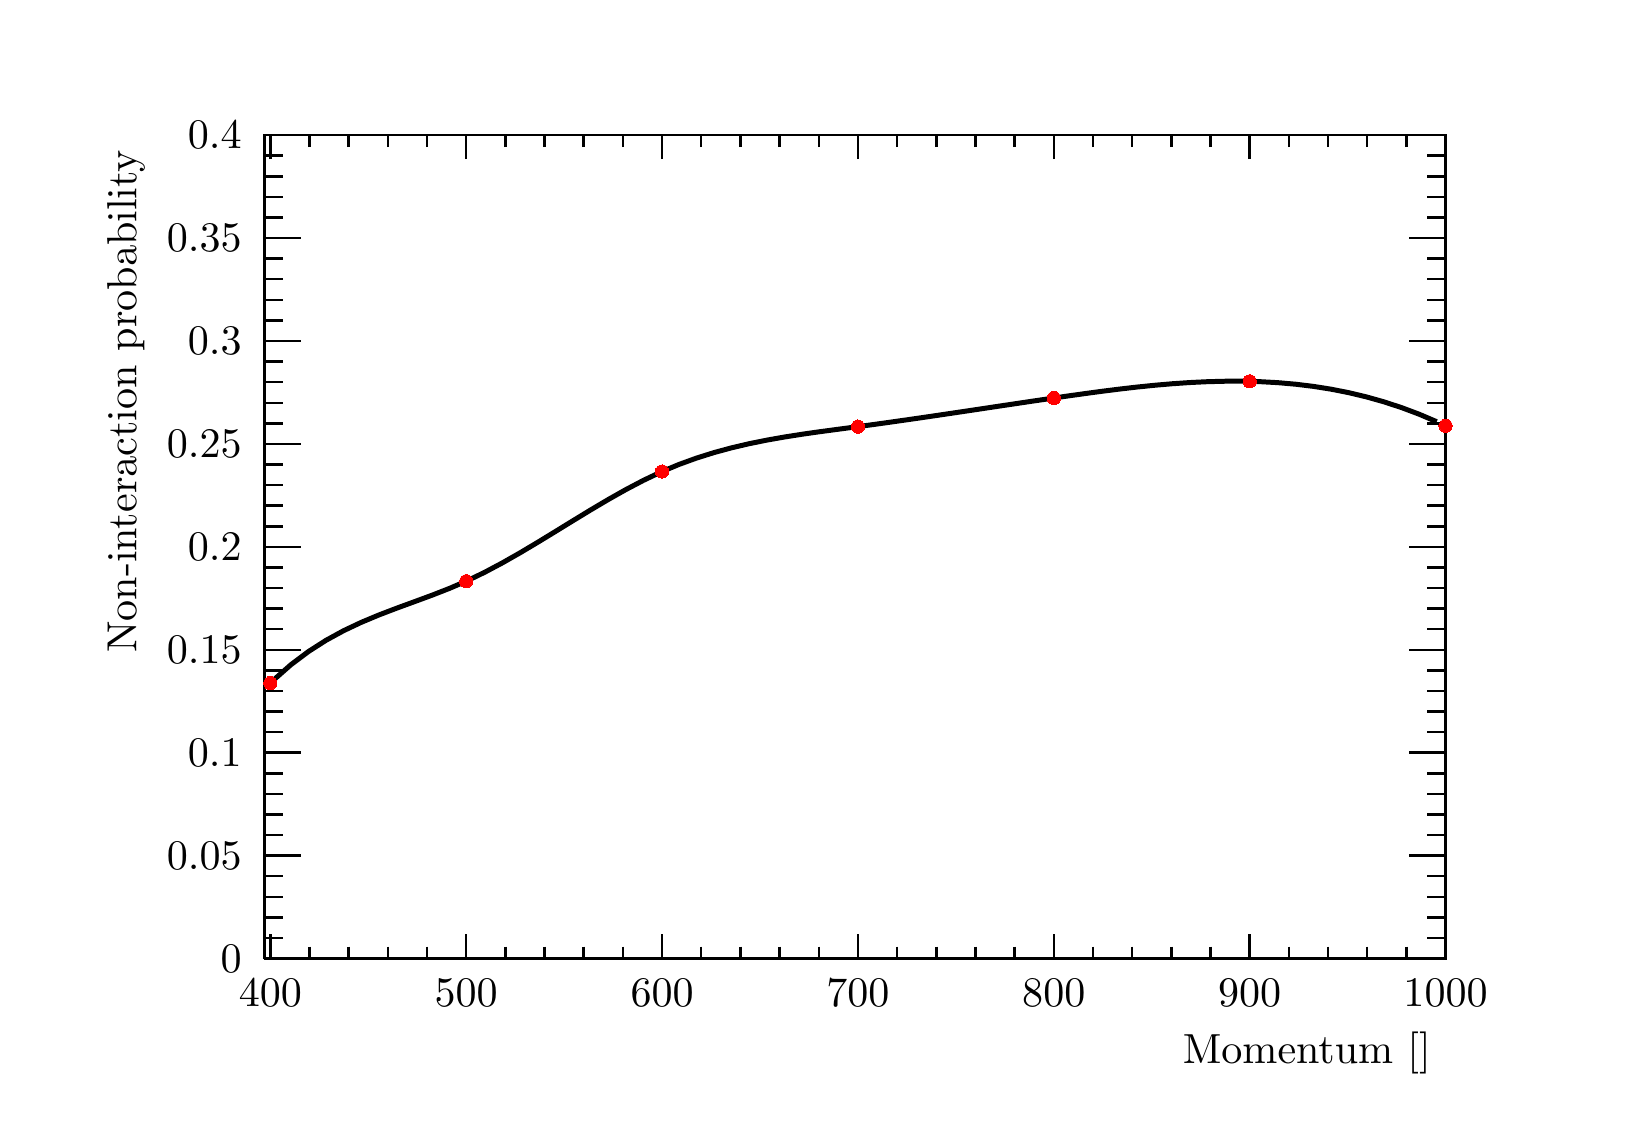
\begin{tikzpicture}
\pgfdeclareplotmark{cross} {
\pgfpathmoveto{\pgfpoint{-0.3\pgfplotmarksize}{\pgfplotmarksize}}
\pgfpathlineto{\pgfpoint{+0.3\pgfplotmarksize}{\pgfplotmarksize}}
\pgfpathlineto{\pgfpoint{+0.3\pgfplotmarksize}{0.3\pgfplotmarksize}}
\pgfpathlineto{\pgfpoint{+1\pgfplotmarksize}{0.3\pgfplotmarksize}}
\pgfpathlineto{\pgfpoint{+1\pgfplotmarksize}{-0.3\pgfplotmarksize}}
\pgfpathlineto{\pgfpoint{+0.3\pgfplotmarksize}{-0.3\pgfplotmarksize}}
\pgfpathlineto{\pgfpoint{+0.3\pgfplotmarksize}{-1.\pgfplotmarksize}}
\pgfpathlineto{\pgfpoint{-0.3\pgfplotmarksize}{-1.\pgfplotmarksize}}
\pgfpathlineto{\pgfpoint{-0.3\pgfplotmarksize}{-0.3\pgfplotmarksize}}
\pgfpathlineto{\pgfpoint{-1.\pgfplotmarksize}{-0.3\pgfplotmarksize}}
\pgfpathlineto{\pgfpoint{-1.\pgfplotmarksize}{0.3\pgfplotmarksize}}
\pgfpathlineto{\pgfpoint{-0.3\pgfplotmarksize}{0.3\pgfplotmarksize}}
\pgfpathclose
\pgfusepathqstroke
}
\pgfdeclareplotmark{cross*} {
\pgfpathmoveto{\pgfpoint{-0.3\pgfplotmarksize}{\pgfplotmarksize}}
\pgfpathlineto{\pgfpoint{+0.3\pgfplotmarksize}{\pgfplotmarksize}}
\pgfpathlineto{\pgfpoint{+0.3\pgfplotmarksize}{0.3\pgfplotmarksize}}
\pgfpathlineto{\pgfpoint{+1\pgfplotmarksize}{0.3\pgfplotmarksize}}
\pgfpathlineto{\pgfpoint{+1\pgfplotmarksize}{-0.3\pgfplotmarksize}}
\pgfpathlineto{\pgfpoint{+0.3\pgfplotmarksize}{-0.3\pgfplotmarksize}}
\pgfpathlineto{\pgfpoint{+0.3\pgfplotmarksize}{-1.\pgfplotmarksize}}
\pgfpathlineto{\pgfpoint{-0.3\pgfplotmarksize}{-1.\pgfplotmarksize}}
\pgfpathlineto{\pgfpoint{-0.3\pgfplotmarksize}{-0.3\pgfplotmarksize}}
\pgfpathlineto{\pgfpoint{-1.\pgfplotmarksize}{-0.3\pgfplotmarksize}}
\pgfpathlineto{\pgfpoint{-1.\pgfplotmarksize}{0.3\pgfplotmarksize}}
\pgfpathlineto{\pgfpoint{-0.3\pgfplotmarksize}{0.3\pgfplotmarksize}}
\pgfpathclose
\pgfusepathqfillstroke
}
\pgfdeclareplotmark{newstar} {
\pgfpathmoveto{\pgfqpoint{0pt}{\pgfplotmarksize}}
\pgfpathlineto{\pgfqpointpolar{44}{0.5\pgfplotmarksize}}
\pgfpathlineto{\pgfqpointpolar{18}{\pgfplotmarksize}}
\pgfpathlineto{\pgfqpointpolar{-20}{0.5\pgfplotmarksize}}
\pgfpathlineto{\pgfqpointpolar{-54}{\pgfplotmarksize}}
\pgfpathlineto{\pgfqpointpolar{-90}{0.5\pgfplotmarksize}}
\pgfpathlineto{\pgfqpointpolar{234}{\pgfplotmarksize}}
\pgfpathlineto{\pgfqpointpolar{198}{0.5\pgfplotmarksize}}
\pgfpathlineto{\pgfqpointpolar{162}{\pgfplotmarksize}}
\pgfpathlineto{\pgfqpointpolar{134}{0.5\pgfplotmarksize}}
\pgfpathclose
\pgfusepathqstroke
}
\pgfdeclareplotmark{newstar*} {
\pgfpathmoveto{\pgfqpoint{0pt}{\pgfplotmarksize}}
\pgfpathlineto{\pgfqpointpolar{44}{0.5\pgfplotmarksize}}
\pgfpathlineto{\pgfqpointpolar{18}{\pgfplotmarksize}}
\pgfpathlineto{\pgfqpointpolar{-20}{0.5\pgfplotmarksize}}
\pgfpathlineto{\pgfqpointpolar{-54}{\pgfplotmarksize}}
\pgfpathlineto{\pgfqpointpolar{-90}{0.5\pgfplotmarksize}}
\pgfpathlineto{\pgfqpointpolar{234}{\pgfplotmarksize}}
\pgfpathlineto{\pgfqpointpolar{198}{0.5\pgfplotmarksize}}
\pgfpathlineto{\pgfqpointpolar{162}{\pgfplotmarksize}}
\pgfpathlineto{\pgfqpointpolar{134}{0.5\pgfplotmarksize}}
\pgfpathclose
\pgfusepathqfillstroke
}
\definecolor{c}{rgb}{1,1,1};
\draw [color=c, fill=c] (0,0) rectangle (20,13.5806);
\draw [color=c, fill=c] (3,1.76548) rectangle (18,12.2225);
\definecolor{c}{rgb}{0,0,0};
\draw [c,line width=0.9] (3,1.76548) -- (3,12.2225) -- (18,12.2225) -- (18,1.76548) -- (3,1.76548);
\definecolor{c}{rgb}{1,1,1};
\draw [color=c, fill=c] (0,0) rectangle (20,13.5806);
\draw [color=c, fill=c] (3,1.76548) rectangle (18,12.2225);
\definecolor{c}{rgb}{0,0,0};
\draw [c,line width=0.9] (3,1.76548) -- (3,12.2225) -- (18,12.2225) -- (18,1.76548) -- (3,1.76548);
\draw [c,line width=1.8] (3.11194,5.29942) -- (3.33582,5.49684) -- (3.5597,5.66493) -- (3.78358,5.80797) -- (4.00746,5.93022) -- (4.23134,6.03596) -- (4.45522,6.12947) -- (4.6791,6.21501) -- (4.90299,6.29688) -- (5.12687,6.37933) -- (5.35075,6.46664)
 -- (5.57463,6.5631) -- (5.79851,6.67165) -- (6.02239,6.79084) -- (6.24627,6.91826) -- (6.47015,7.05151) -- (6.69403,7.18817) -- (6.91791,7.32585) -- (7.14179,7.46214) -- (7.36567,7.59463) -- (7.58955,7.72092) -- (7.81343,7.8386) -- (8.03731,7.94527)
 -- (8.26119,8.03905) -- (8.48507,8.12051) -- (8.70895,8.19097) -- (8.93284,8.25173) -- (9.15672,8.30411) -- (9.3806,8.34943) -- (9.60448,8.38897) -- (9.82836,8.42407) -- (10.0522,8.45603) -- (10.2761,8.48616) -- (10.5,8.51576) -- (10.7239,8.54602)
 -- (10.9478,8.57717) -- (11.1716,8.60908) -- (11.3955,8.64161) -- (11.6194,8.67461) -- (11.8433,8.70796) -- (12.0672,8.74152) -- (12.291,8.77514) -- (12.5149,8.80869) -- (12.7388,8.84204) -- (12.9627,8.87504) -- (13.1866,8.90753) --
 (13.4104,8.93912) -- (13.6343,8.96929) -- (13.8582,8.99753) -- (14.0821,9.02332);
\draw [c,line width=1.8] (14.0821,9.02332) -- (14.306,9.04613) -- (14.5299,9.06545) -- (14.7537,9.08076) -- (14.9776,9.09154) -- (15.2015,9.09727) -- (15.4254,9.09743) -- (15.6493,9.09151) -- (15.8731,9.07897) -- (16.097,9.05931) -- (16.3209,9.03201)
 -- (16.5448,8.99655) -- (16.7687,8.9524) -- (16.9925,8.89905) -- (17.2164,8.83598) -- (17.4403,8.76267) -- (17.6642,8.67861) -- (17.8881,8.58326);
\draw [c,line width=0.9] (3,1.76548) -- (18,1.76548);
\draw [c,line width=0.9] (3.07463,2.07104) -- (3.07463,1.76548);
\draw [c,line width=0.9] (3.57214,1.91826) -- (3.57214,1.76548);
\draw [c,line width=0.9] (4.06965,1.91826) -- (4.06965,1.76548);
\draw [c,line width=0.9] (4.56716,1.91826) -- (4.56716,1.76548);
\draw [c,line width=0.9] (5.06468,1.91826) -- (5.06468,1.76548);
\draw [c,line width=0.9] (5.56219,2.07104) -- (5.56219,1.76548);
\draw [c,line width=0.9] (6.0597,1.91826) -- (6.0597,1.76548);
\draw [c,line width=0.9] (6.55721,1.91826) -- (6.55721,1.76548);
\draw [c,line width=0.9] (7.05473,1.91826) -- (7.05473,1.76548);
\draw [c,line width=0.9] (7.55224,1.91826) -- (7.55224,1.76548);
\draw [c,line width=0.9] (8.04975,2.07104) -- (8.04975,1.76548);
\draw [c,line width=0.9] (8.54726,1.91826) -- (8.54726,1.76548);
\draw [c,line width=0.9] (9.04478,1.91826) -- (9.04478,1.76548);
\draw [c,line width=0.9] (9.54229,1.91826) -- (9.54229,1.76548);
\draw [c,line width=0.9] (10.0398,1.91826) -- (10.0398,1.76548);
\draw [c,line width=0.9] (10.5373,2.07104) -- (10.5373,1.76548);
\draw [c,line width=0.9] (11.0348,1.91826) -- (11.0348,1.76548);
\draw [c,line width=0.9] (11.5323,1.91826) -- (11.5323,1.76548);
\draw [c,line width=0.9] (12.0299,1.91826) -- (12.0299,1.76548);
\draw [c,line width=0.9] (12.5274,1.91826) -- (12.5274,1.76548);
\draw [c,line width=0.9] (13.0249,2.07104) -- (13.0249,1.76548);
\draw [c,line width=0.9] (13.5224,1.91826) -- (13.5224,1.76548);
\draw [c,line width=0.9] (14.0199,1.91826) -- (14.0199,1.76548);
\draw [c,line width=0.9] (14.5174,1.91826) -- (14.5174,1.76548);
\draw [c,line width=0.9] (15.0149,1.91826) -- (15.0149,1.76548);
\draw [c,line width=0.9] (15.5124,2.07104) -- (15.5124,1.76548);
\draw [c,line width=0.9] (16.01,1.91826) -- (16.01,1.76548);
\draw [c,line width=0.9] (16.5075,1.91826) -- (16.5075,1.76548);
\draw [c,line width=0.9] (17.005,1.91826) -- (17.005,1.76548);
\draw [c,line width=0.9] (17.5025,1.91826) -- (17.5025,1.76548);
\draw [c,line width=0.9] (18,2.07104) -- (18,1.76548);
\draw [c,line width=0.9] (3.07463,2.07104) -- (3.07463,1.76548);
\draw [anchor=base] (3.07463,1.15435) node[scale=1.52078, color=c, rotate=0]{400};
\draw [anchor=base] (5.56219,1.15435) node[scale=1.52078, color=c, rotate=0]{500};
\draw [anchor=base] (8.04975,1.15435) node[scale=1.52078, color=c, rotate=0]{600};
\draw [anchor=base] (10.5373,1.15435) node[scale=1.52078, color=c, rotate=0]{700};
\draw [anchor=base] (13.0249,1.15435) node[scale=1.52078, color=c, rotate=0]{800};
\draw [anchor=base] (15.5124,1.15435) node[scale=1.52078, color=c, rotate=0]{900};
\draw [anchor=base] (18,1.15435) node[scale=1.52078, color=c, rotate=0]{1000};
\draw [anchor= east] (18,0.570385) node[scale=1.52078, color=c, rotate=0]{Momentum [\si{\MeV\per\clight}]};
\draw [c,line width=0.9] (3,12.2225) -- (18,12.2225);
\draw [c,line width=0.9] (3.07463,11.917) -- (3.07463,12.2225);
\draw [c,line width=0.9] (3.57214,12.0698) -- (3.57214,12.2225);
\draw [c,line width=0.9] (4.06965,12.0698) -- (4.06965,12.2225);
\draw [c,line width=0.9] (4.56716,12.0698) -- (4.56716,12.2225);
\draw [c,line width=0.9] (5.06468,12.0698) -- (5.06468,12.2225);
\draw [c,line width=0.9] (5.56219,11.917) -- (5.56219,12.2225);
\draw [c,line width=0.9] (6.0597,12.0698) -- (6.0597,12.2225);
\draw [c,line width=0.9] (6.55721,12.0698) -- (6.55721,12.2225);
\draw [c,line width=0.9] (7.05473,12.0698) -- (7.05473,12.2225);
\draw [c,line width=0.9] (7.55224,12.0698) -- (7.55224,12.2225);
\draw [c,line width=0.9] (8.04975,11.917) -- (8.04975,12.2225);
\draw [c,line width=0.9] (8.54726,12.0698) -- (8.54726,12.2225);
\draw [c,line width=0.9] (9.04478,12.0698) -- (9.04478,12.2225);
\draw [c,line width=0.9] (9.54229,12.0698) -- (9.54229,12.2225);
\draw [c,line width=0.9] (10.0398,12.0698) -- (10.0398,12.2225);
\draw [c,line width=0.9] (10.5373,11.917) -- (10.5373,12.2225);
\draw [c,line width=0.9] (11.0348,12.0698) -- (11.0348,12.2225);
\draw [c,line width=0.9] (11.5323,12.0698) -- (11.5323,12.2225);
\draw [c,line width=0.9] (12.0299,12.0698) -- (12.0299,12.2225);
\draw [c,line width=0.9] (12.5274,12.0698) -- (12.5274,12.2225);
\draw [c,line width=0.9] (13.0249,11.917) -- (13.0249,12.2225);
\draw [c,line width=0.9] (13.5224,12.0698) -- (13.5224,12.2225);
\draw [c,line width=0.9] (14.0199,12.0698) -- (14.0199,12.2225);
\draw [c,line width=0.9] (14.5174,12.0698) -- (14.5174,12.2225);
\draw [c,line width=0.9] (15.0149,12.0698) -- (15.0149,12.2225);
\draw [c,line width=0.9] (15.5124,11.917) -- (15.5124,12.2225);
\draw [c,line width=0.9] (16.01,12.0698) -- (16.01,12.2225);
\draw [c,line width=0.9] (16.5075,12.0698) -- (16.5075,12.2225);
\draw [c,line width=0.9] (17.005,12.0698) -- (17.005,12.2225);
\draw [c,line width=0.9] (17.5025,12.0698) -- (17.5025,12.2225);
\draw [c,line width=0.9] (18,11.917) -- (18,12.2225);
\draw [c,line width=0.9] (3.07463,11.917) -- (3.07463,12.2225);
\draw [c,line width=0.9] (3,1.76548) -- (3,12.2225);
\draw [c,line width=0.9] (3.462,1.76548) -- (3,1.76548);
\draw [c,line width=0.9] (3.231,2.0269) -- (3,2.0269);
\draw [c,line width=0.9] (3.231,2.28833) -- (3,2.28833);
\draw [c,line width=0.9] (3.231,2.54976) -- (3,2.54976);
\draw [c,line width=0.9] (3.231,2.81118) -- (3,2.81118);
\draw [c,line width=0.9] (3.462,3.07261) -- (3,3.07261);
\draw [c,line width=0.9] (3.231,3.33404) -- (3,3.33404);
\draw [c,line width=0.9] (3.231,3.59546) -- (3,3.59546);
\draw [c,line width=0.9] (3.231,3.85689) -- (3,3.85689);
\draw [c,line width=0.9] (3.231,4.11832) -- (3,4.11832);
\draw [c,line width=0.9] (3.462,4.37974) -- (3,4.37974);
\draw [c,line width=0.9] (3.231,4.64117) -- (3,4.64117);
\draw [c,line width=0.9] (3.231,4.9026) -- (3,4.9026);
\draw [c,line width=0.9] (3.231,5.16402) -- (3,5.16402);
\draw [c,line width=0.9] (3.231,5.42545) -- (3,5.42545);
\draw [c,line width=0.9] (3.462,5.68688) -- (3,5.68688);
\draw [c,line width=0.9] (3.231,5.9483) -- (3,5.9483);
\draw [c,line width=0.9] (3.231,6.20973) -- (3,6.20973);
\draw [c,line width=0.9] (3.231,6.47116) -- (3,6.47116);
\draw [c,line width=0.9] (3.231,6.73258) -- (3,6.73258);
\draw [c,line width=0.9] (3.462,6.99401) -- (3,6.99401);
\draw [c,line width=0.9] (3.231,7.25543) -- (3,7.25543);
\draw [c,line width=0.9] (3.231,7.51686) -- (3,7.51686);
\draw [c,line width=0.9] (3.231,7.77829) -- (3,7.77829);
\draw [c,line width=0.9] (3.231,8.03971) -- (3,8.03971);
\draw [c,line width=0.9] (3.462,8.30114) -- (3,8.30114);
\draw [c,line width=0.9] (3.231,8.56257) -- (3,8.56257);
\draw [c,line width=0.9] (3.231,8.82399) -- (3,8.82399);
\draw [c,line width=0.9] (3.231,9.08542) -- (3,9.08542);
\draw [c,line width=0.9] (3.231,9.34685) -- (3,9.34685);
\draw [c,line width=0.9] (3.462,9.60827) -- (3,9.60827);
\draw [c,line width=0.9] (3.231,9.8697) -- (3,9.8697);
\draw [c,line width=0.9] (3.231,10.1311) -- (3,10.1311);
\draw [c,line width=0.9] (3.231,10.3926) -- (3,10.3926);
\draw [c,line width=0.9] (3.231,10.654) -- (3,10.654);
\draw [c,line width=0.9] (3.462,10.9154) -- (3,10.9154);
\draw [c,line width=0.9] (3.231,11.1768) -- (3,11.1768);
\draw [c,line width=0.9] (3.231,11.4383) -- (3,11.4383);
\draw [c,line width=0.9] (3.231,11.6997) -- (3,11.6997);
\draw [c,line width=0.9] (3.231,11.9611) -- (3,11.9611);
\draw [c,line width=0.9] (3.462,12.2225) -- (3,12.2225);
\draw [anchor= east] (2.9,1.76548) node[scale=1.52078, color=c, rotate=0]{0};
\draw [anchor= east] (2.9,3.07261) node[scale=1.52078, color=c, rotate=0]{0.05};
\draw [anchor= east] (2.9,4.37974) node[scale=1.52078, color=c, rotate=0]{0.1};
\draw [anchor= east] (2.9,5.68688) node[scale=1.52078, color=c, rotate=0]{0.15};
\draw [anchor= east] (2.9,6.99401) node[scale=1.52078, color=c, rotate=0]{0.2};
\draw [anchor= east] (2.9,8.30114) node[scale=1.52078, color=c, rotate=0]{0.25};
\draw [anchor= east] (2.9,9.60827) node[scale=1.52078, color=c, rotate=0]{0.3};
\draw [anchor= east] (2.9,10.9154) node[scale=1.52078, color=c, rotate=0]{0.35};
\draw [anchor= east] (2.9,12.2225) node[scale=1.52078, color=c, rotate=0]{0.4};
\draw [anchor= east] (1.24,12.2225) node[scale=1.52078, color=c, rotate=90]{ Non-interaction probability};
\draw [c,line width=0.9] (18,1.76548) -- (18,12.2225);
\draw [c,line width=0.9] (17.538,1.76548) -- (18,1.76548);
\draw [c,line width=0.9] (17.769,2.0269) -- (18,2.0269);
\draw [c,line width=0.9] (17.769,2.28833) -- (18,2.28833);
\draw [c,line width=0.9] (17.769,2.54976) -- (18,2.54976);
\draw [c,line width=0.9] (17.769,2.81118) -- (18,2.81118);
\draw [c,line width=0.9] (17.538,3.07261) -- (18,3.07261);
\draw [c,line width=0.9] (17.769,3.33404) -- (18,3.33404);
\draw [c,line width=0.9] (17.769,3.59546) -- (18,3.59546);
\draw [c,line width=0.9] (17.769,3.85689) -- (18,3.85689);
\draw [c,line width=0.9] (17.769,4.11832) -- (18,4.11832);
\draw [c,line width=0.9] (17.538,4.37974) -- (18,4.37974);
\draw [c,line width=0.9] (17.769,4.64117) -- (18,4.64117);
\draw [c,line width=0.9] (17.769,4.9026) -- (18,4.9026);
\draw [c,line width=0.9] (17.769,5.16402) -- (18,5.16402);
\draw [c,line width=0.9] (17.769,5.42545) -- (18,5.42545);
\draw [c,line width=0.9] (17.538,5.68688) -- (18,5.68688);
\draw [c,line width=0.9] (17.769,5.9483) -- (18,5.9483);
\draw [c,line width=0.9] (17.769,6.20973) -- (18,6.20973);
\draw [c,line width=0.9] (17.769,6.47116) -- (18,6.47116);
\draw [c,line width=0.9] (17.769,6.73258) -- (18,6.73258);
\draw [c,line width=0.9] (17.538,6.99401) -- (18,6.99401);
\draw [c,line width=0.9] (17.769,7.25543) -- (18,7.25543);
\draw [c,line width=0.9] (17.769,7.51686) -- (18,7.51686);
\draw [c,line width=0.9] (17.769,7.77829) -- (18,7.77829);
\draw [c,line width=0.9] (17.769,8.03971) -- (18,8.03971);
\draw [c,line width=0.9] (17.538,8.30114) -- (18,8.30114);
\draw [c,line width=0.9] (17.769,8.56257) -- (18,8.56257);
\draw [c,line width=0.9] (17.769,8.82399) -- (18,8.82399);
\draw [c,line width=0.9] (17.769,9.08542) -- (18,9.08542);
\draw [c,line width=0.9] (17.769,9.34685) -- (18,9.34685);
\draw [c,line width=0.9] (17.538,9.60827) -- (18,9.60827);
\draw [c,line width=0.9] (17.769,9.8697) -- (18,9.8697);
\draw [c,line width=0.9] (17.769,10.1311) -- (18,10.1311);
\draw [c,line width=0.9] (17.769,10.3926) -- (18,10.3926);
\draw [c,line width=0.9] (17.769,10.654) -- (18,10.654);
\draw [c,line width=0.9] (17.538,10.9154) -- (18,10.9154);
\draw [c,line width=0.9] (17.769,11.1768) -- (18,11.1768);
\draw [c,line width=0.9] (17.769,11.4383) -- (18,11.4383);
\draw [c,line width=0.9] (17.769,11.6997) -- (18,11.6997);
\draw [c,line width=0.9] (17.769,11.9611) -- (18,11.9611);
\draw [c,line width=0.9] (17.538,12.2225) -- (18,12.2225);
\definecolor{c}{rgb}{1,0,0};
\foreach \P in {(3.07463,5.26336), (5.56219,6.55743), (8.04975,7.95083), (10.5373,8.52074), (13.0249,8.88412), (15.5124,9.09588), (18,8.5312)}{\draw[mark options={color=c,fill=c},mark size=2.402402pt, line width=0.000000pt, mark=*] plot coordinates
 {\P};}
\end{tikzpicture}

	\end{adjustbox}
	\caption[Non-interaction probability for a charged pion travelling through the ND-GAr ECAL as a function of momentum]{Non-interaction probability for a charged pion travelling through the ND-GAr ECAL as a function of momentum. Points derived from simulation are shown in red through which a spline is plotted (black).}
	\label{fig:interactionSpline}
\end{figure}

Charged pions with $p>\SI{1}{\GeV\per\clight}$ are considered to have passed into the muon identification system. 
This system has a thickness of approximately 2 interaction lengths for charged pions.
If the pion interacts in the muon identification system, it is correctly identified.
Therefore, these pions have a probability of $e^{-3}$ to be misidentified as muons.

Finally, it is assumed that the detector is able to perfectly sign select particles such as charged pions and muons.

\section{Measurements of pion multiplicity}
\label{sec:dune_ndrwt:pionMulti}

The parametrised reconstruction detailed in \citesec{sec:dune_ndrwt:simDetails} is used to select muon neutrino events and classify their final state.
An event is considered to be a \numu or \anumu charged current event if there is a reconstructed muon in the final state which has a track length perpendicular to the magnetic field of over \SI{1}{\metre}.
Alternatively, if the reconstructed muon exits the HPgTPC and ranges out in the ECAL it is also reconstructed as a \numu CC event.
The term `ranging out' here refers to a particle stopping in the detector without interacting.
The muon is judged to have ranged out in the ECAL if it has a momentum of less than \SI{380}{\MeV\per\clight} when exiting the HPgTPC. 

\citefig{fig:confusMatPi} shows the confusion matrices produced using the above selection for both forward and reverse horn currents. 
Here one can see that, for all final states, the correct final state is reconstructed at least 88\% of the time.
%The largest probability for miscategorised events are NC events where single charged pion is wrongly reconstructed as a muon and the whole event is categorised as a $0\pi$ final state.
%However, one can see from \citefig{fig:eventCats}, that these represent a very small fraction of the total number of events.

\begin{figure}[h]
	\begin{minipage}[t]{.5\linewidth}
		\begin{adjustbox}{max totalsize=\linewidth, center}
			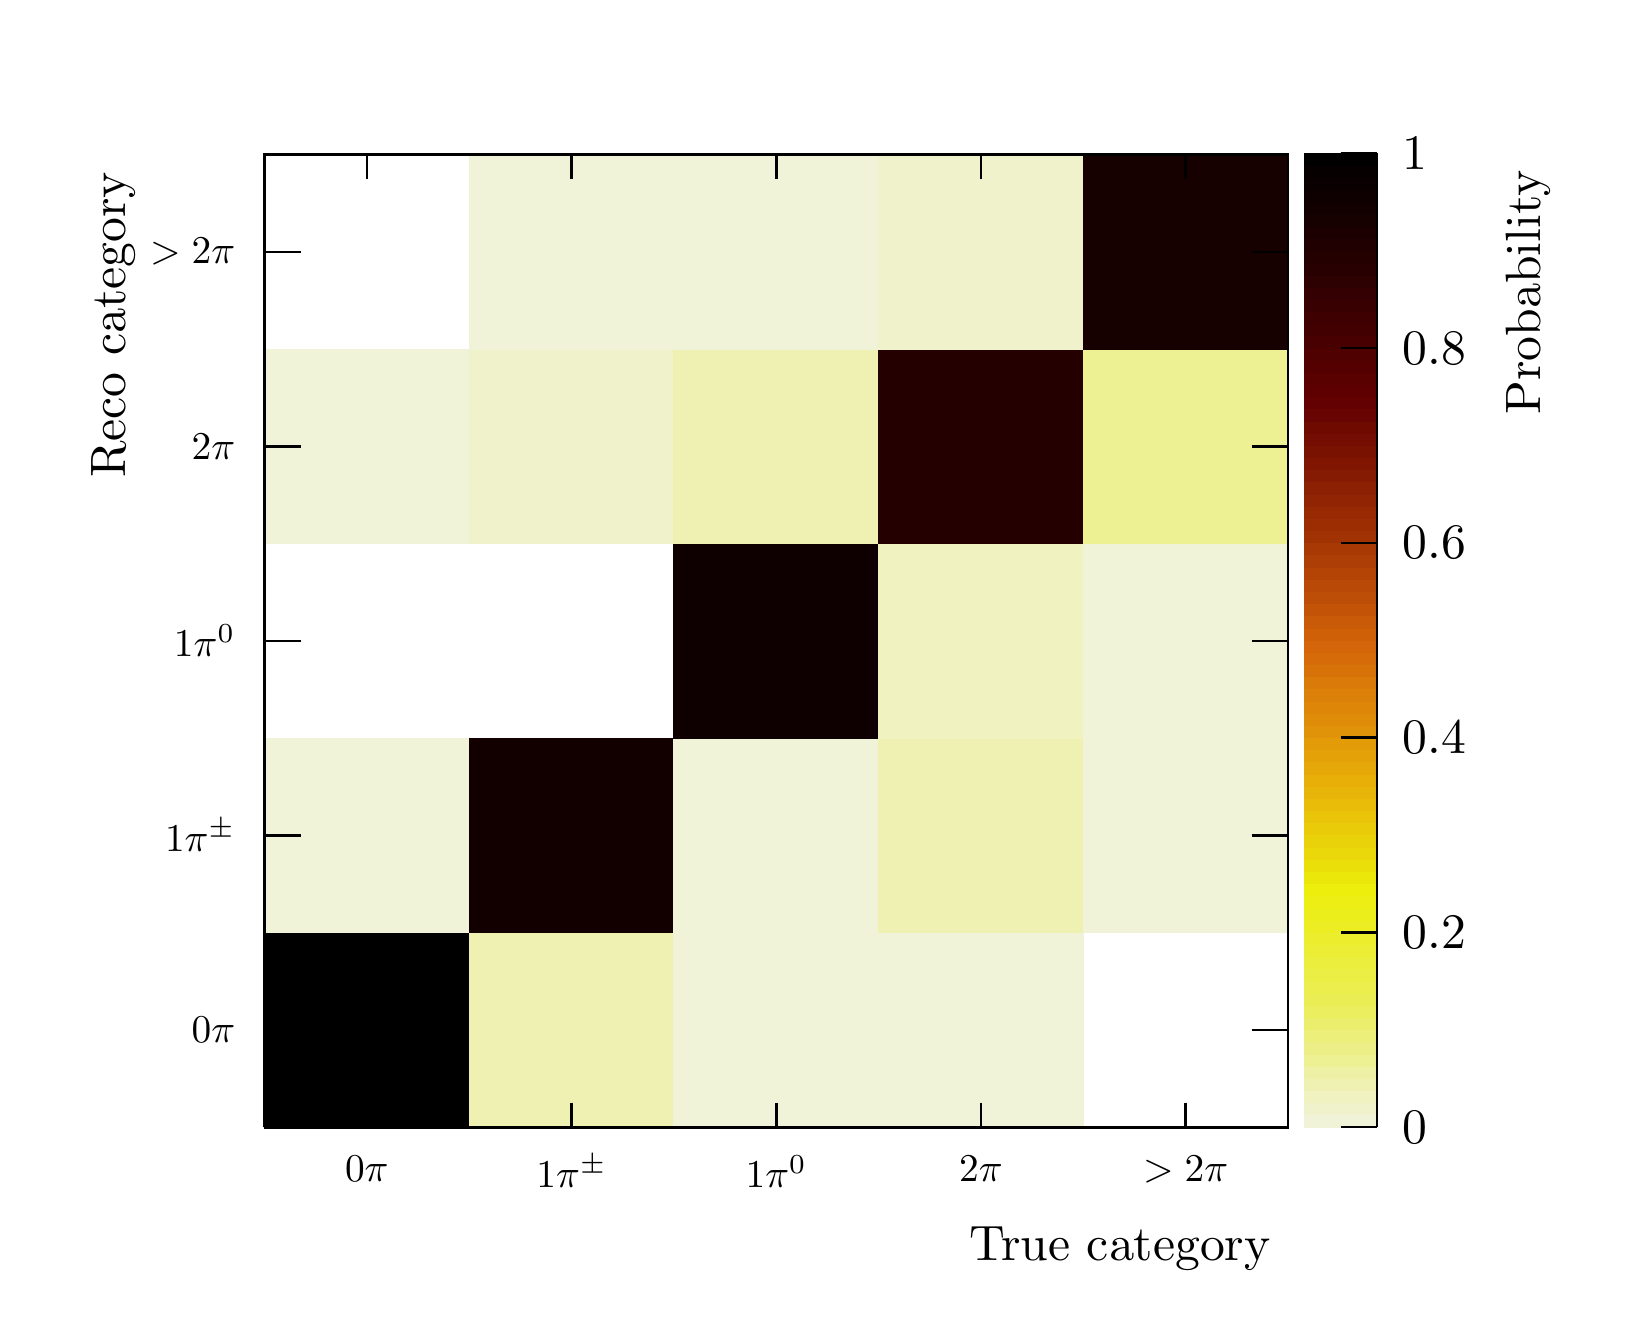
\begin{tikzpicture}
\pgfdeclareplotmark{cross} {
\pgfpathmoveto{\pgfpoint{-0.3\pgfplotmarksize}{\pgfplotmarksize}}
\pgfpathlineto{\pgfpoint{+0.3\pgfplotmarksize}{\pgfplotmarksize}}
\pgfpathlineto{\pgfpoint{+0.3\pgfplotmarksize}{0.3\pgfplotmarksize}}
\pgfpathlineto{\pgfpoint{+1\pgfplotmarksize}{0.3\pgfplotmarksize}}
\pgfpathlineto{\pgfpoint{+1\pgfplotmarksize}{-0.3\pgfplotmarksize}}
\pgfpathlineto{\pgfpoint{+0.3\pgfplotmarksize}{-0.3\pgfplotmarksize}}
\pgfpathlineto{\pgfpoint{+0.3\pgfplotmarksize}{-1.\pgfplotmarksize}}
\pgfpathlineto{\pgfpoint{-0.3\pgfplotmarksize}{-1.\pgfplotmarksize}}
\pgfpathlineto{\pgfpoint{-0.3\pgfplotmarksize}{-0.3\pgfplotmarksize}}
\pgfpathlineto{\pgfpoint{-1.\pgfplotmarksize}{-0.3\pgfplotmarksize}}
\pgfpathlineto{\pgfpoint{-1.\pgfplotmarksize}{0.3\pgfplotmarksize}}
\pgfpathlineto{\pgfpoint{-0.3\pgfplotmarksize}{0.3\pgfplotmarksize}}
\pgfpathclose
\pgfusepathqstroke
}
\pgfdeclareplotmark{cross*} {
\pgfpathmoveto{\pgfpoint{-0.3\pgfplotmarksize}{\pgfplotmarksize}}
\pgfpathlineto{\pgfpoint{+0.3\pgfplotmarksize}{\pgfplotmarksize}}
\pgfpathlineto{\pgfpoint{+0.3\pgfplotmarksize}{0.3\pgfplotmarksize}}
\pgfpathlineto{\pgfpoint{+1\pgfplotmarksize}{0.3\pgfplotmarksize}}
\pgfpathlineto{\pgfpoint{+1\pgfplotmarksize}{-0.3\pgfplotmarksize}}
\pgfpathlineto{\pgfpoint{+0.3\pgfplotmarksize}{-0.3\pgfplotmarksize}}
\pgfpathlineto{\pgfpoint{+0.3\pgfplotmarksize}{-1.\pgfplotmarksize}}
\pgfpathlineto{\pgfpoint{-0.3\pgfplotmarksize}{-1.\pgfplotmarksize}}
\pgfpathlineto{\pgfpoint{-0.3\pgfplotmarksize}{-0.3\pgfplotmarksize}}
\pgfpathlineto{\pgfpoint{-1.\pgfplotmarksize}{-0.3\pgfplotmarksize}}
\pgfpathlineto{\pgfpoint{-1.\pgfplotmarksize}{0.3\pgfplotmarksize}}
\pgfpathlineto{\pgfpoint{-0.3\pgfplotmarksize}{0.3\pgfplotmarksize}}
\pgfpathclose
\pgfusepathqfillstroke
}
\pgfdeclareplotmark{newstar} {
\pgfpathmoveto{\pgfqpoint{0pt}{\pgfplotmarksize}}
\pgfpathlineto{\pgfqpointpolar{44}{0.5\pgfplotmarksize}}
\pgfpathlineto{\pgfqpointpolar{18}{\pgfplotmarksize}}
\pgfpathlineto{\pgfqpointpolar{-20}{0.5\pgfplotmarksize}}
\pgfpathlineto{\pgfqpointpolar{-54}{\pgfplotmarksize}}
\pgfpathlineto{\pgfqpointpolar{-90}{0.5\pgfplotmarksize}}
\pgfpathlineto{\pgfqpointpolar{234}{\pgfplotmarksize}}
\pgfpathlineto{\pgfqpointpolar{198}{0.5\pgfplotmarksize}}
\pgfpathlineto{\pgfqpointpolar{162}{\pgfplotmarksize}}
\pgfpathlineto{\pgfqpointpolar{134}{0.5\pgfplotmarksize}}
\pgfpathclose
\pgfusepathqstroke
}
\pgfdeclareplotmark{newstar*} {
\pgfpathmoveto{\pgfqpoint{0pt}{\pgfplotmarksize}}
\pgfpathlineto{\pgfqpointpolar{44}{0.5\pgfplotmarksize}}
\pgfpathlineto{\pgfqpointpolar{18}{\pgfplotmarksize}}
\pgfpathlineto{\pgfqpointpolar{-20}{0.5\pgfplotmarksize}}
\pgfpathlineto{\pgfqpointpolar{-54}{\pgfplotmarksize}}
\pgfpathlineto{\pgfqpointpolar{-90}{0.5\pgfplotmarksize}}
\pgfpathlineto{\pgfqpointpolar{234}{\pgfplotmarksize}}
\pgfpathlineto{\pgfqpointpolar{198}{0.5\pgfplotmarksize}}
\pgfpathlineto{\pgfqpointpolar{162}{\pgfplotmarksize}}
\pgfpathlineto{\pgfqpointpolar{134}{0.5\pgfplotmarksize}}
\pgfpathclose
\pgfusepathqfillstroke
}
\definecolor{c}{rgb}{1,1,1};
\draw [color=c, fill=c] (0,0) rectangle (20,16.0446);
\draw [color=c, fill=c] (3,2.08579) rectangle (16,14.4401);
\definecolor{c}{rgb}{0,0,0};
\draw [c,line width=0.9] (3,2.08579) -- (3,14.4401) -- (16,14.4401) -- (16,2.08579) -- (3,2.08579);
\definecolor{c}{rgb}{1,1,1};
\draw [color=c, fill=c] (3,2.08579) rectangle (16,14.4401);
\definecolor{c}{rgb}{0,0,0};
\draw [c,line width=0.9] (3,2.08579) -- (3,14.4401) -- (16,14.4401) -- (16,2.08579) -- (3,2.08579);
\definecolor{c}{rgb}{0.00551471,0,0.000122549};
\draw [color=c, fill=c] (3,2.08579) rectangle (5.6,4.55666);
\definecolor{c}{rgb}{0.936875,0.945351,0.697027};
\draw [color=c, fill=c] (5.6,2.08579) rectangle (8.2,4.55666);
\definecolor{c}{rgb}{0.945984,0.951044,0.850727};
\draw [color=c, fill=c] (8.2,2.08579) rectangle (10.8,4.55666);
\draw [color=c, fill=c] (10.8,2.08579) rectangle (13.4,4.55666);
\draw [color=c, fill=c] (3,4.55666) rectangle (5.6,7.02752);
\definecolor{c}{rgb}{0.0716912,0,0.00159314};
\draw [color=c, fill=c] (5.6,4.55666) rectangle (8.2,7.02752);
\definecolor{c}{rgb}{0.945984,0.951044,0.850727};
\draw [color=c, fill=c] (8.2,4.55666) rectangle (10.8,7.02752);
\definecolor{c}{rgb}{0.936875,0.945351,0.697027};
\draw [color=c, fill=c] (10.8,4.55666) rectangle (13.4,7.02752);
\definecolor{c}{rgb}{0.945984,0.951044,0.850727};
\draw [color=c, fill=c] (13.4,4.55666) rectangle (16,7.02752);
\definecolor{c}{rgb}{0.0551471,0,0.00122549};
\draw [color=c, fill=c] (8.2,7.02752) rectangle (10.8,9.49838);
\definecolor{c}{rgb}{0.939911,0.947249,0.748261};
\draw [color=c, fill=c] (10.8,7.02752) rectangle (13.4,9.49838);
\definecolor{c}{rgb}{0.945984,0.951044,0.850727};
\draw [color=c, fill=c] (13.4,7.02752) rectangle (16,9.49838);
\draw [color=c, fill=c] (3,9.49838) rectangle (5.6,11.9692);
\definecolor{c}{rgb}{0.942948,0.949146,0.799494};
\draw [color=c, fill=c] (5.6,9.49838) rectangle (8.2,11.9692);
\definecolor{c}{rgb}{0.936875,0.945351,0.697027};
\draw [color=c, fill=c] (8.2,9.49838) rectangle (10.8,11.9692);
\definecolor{c}{rgb}{0.143382,0,0.00318627};
\draw [color=c, fill=c] (10.8,9.49838) rectangle (13.4,11.9692);
\definecolor{c}{rgb}{0.929791,0.940923,0.577483};
\draw [color=c, fill=c] (13.4,9.49838) rectangle (16,11.9692);
\definecolor{c}{rgb}{0.945984,0.951044,0.850727};
\draw [color=c, fill=c] (5.6,11.9692) rectangle (8.2,14.4401);
\draw [color=c, fill=c] (8.2,11.9692) rectangle (10.8,14.4401);
\definecolor{c}{rgb}{0.942948,0.949146,0.799494};
\draw [color=c, fill=c] (10.8,11.9692) rectangle (13.4,14.4401);
\definecolor{c}{rgb}{0.0882353,0,0.00196078};
\draw [color=c, fill=c] (13.4,11.9692) rectangle (16,14.4401);
\definecolor{c}{rgb}{0,0,0};
\draw [c,line width=0.9] (3,2.08579) -- (16,2.08579);
\draw [anchor=north] (4.3,1.90048) node[scale=1.42291, color=c, rotate=0]{$0\pi$};
\draw [anchor=north] (6.9,1.90048) node[scale=1.42291, color=c, rotate=0]{$1\pi^{\pm}$};
\draw [anchor=north] (9.5,1.90048) node[scale=1.42291, color=c, rotate=0]{$1\pi^{0}$};
\draw [anchor=north] (12.1,1.90048) node[scale=1.42291, color=c, rotate=0]{$2\pi$};
\draw [anchor=north] (14.7,1.90048) node[scale=1.42291, color=c, rotate=0]{$>2\pi$};
\draw [c,line width=0.9] (4.3,2.39866) -- (4.3,2.08579);
\draw [c,line width=0.9] (6.9,2.39866) -- (6.9,2.08579);
\draw [c,line width=0.9] (9.5,2.39866) -- (9.5,2.08579);
\draw [c,line width=0.9] (12.1,2.39866) -- (12.1,2.08579);
\draw [c,line width=0.9] (14.7,2.39866) -- (14.7,2.08579);
\draw [c,line width=0.9] (4.3,2.39866) -- (4.3,2.08579);
\draw [c,line width=0.9] (14.7,2.39866) -- (14.7,2.08579);
\draw [anchor= east] (16,0.545515) node[scale=1.7941, color=c, rotate=0]{ True category};
\draw [c,line width=0.9] (3,14.4401) -- (16,14.4401);
\draw [c,line width=0.9] (4.3,14.1272) -- (4.3,14.4401);
\draw [c,line width=0.9] (6.9,14.1272) -- (6.9,14.4401);
\draw [c,line width=0.9] (9.5,14.1272) -- (9.5,14.4401);
\draw [c,line width=0.9] (12.1,14.1272) -- (12.1,14.4401);
\draw [c,line width=0.9] (14.7,14.1272) -- (14.7,14.4401);
\draw [c,line width=0.9] (4.3,14.1272) -- (4.3,14.4401);
\draw [c,line width=0.9] (14.7,14.1272) -- (14.7,14.4401);
\draw [c,line width=0.9] (3,2.08579) -- (3,14.4401);
\draw [anchor= east] (2.805,3.32123) node[scale=1.42291, color=c, rotate=0]{$0\pi$};
\draw [anchor= east] (2.805,5.79209) node[scale=1.42291, color=c, rotate=0]{$1\pi^{\pm}$};
\draw [anchor= east] (2.805,8.26295) node[scale=1.42291, color=c, rotate=0]{$1\pi^{0}$};
\draw [anchor= east] (2.805,10.7338) node[scale=1.42291, color=c, rotate=0]{$2\pi$};
\draw [anchor= east] (2.805,13.2047) node[scale=1.42291, color=c, rotate=0]{$>2\pi$};
\draw [c,line width=0.9] (3.462,3.32123) -- (3,3.32123);
\draw [c,line width=0.9] (3.462,5.79209) -- (3,5.79209);
\draw [c,line width=0.9] (3.462,8.26295) -- (3,8.26295);
\draw [c,line width=0.9] (3.462,10.7338) -- (3,10.7338);
\draw [c,line width=0.9] (3.462,13.2047) -- (3,13.2047);
\draw [c,line width=0.9] (3.462,3.32123) -- (3,3.32123);
\draw [c,line width=0.9] (3.462,13.2047) -- (3,13.2047);
\draw [anchor= east] (1.08,14.4401) node[scale=1.7941, color=c, rotate=90]{ Reco category};
\draw [c,line width=0.9] (16,2.08579) -- (16,14.4401);
\draw [c,line width=0.9] (15.538,3.32123) -- (16,3.32123);
\draw [c,line width=0.9] (15.538,5.79209) -- (16,5.79209);
\draw [c,line width=0.9] (15.538,8.26295) -- (16,8.26295);
\draw [c,line width=0.9] (15.538,10.7338) -- (16,10.7338);
\draw [c,line width=0.9] (15.538,13.2047) -- (16,13.2047);
\draw [c,line width=0.9] (15.538,3.32123) -- (16,3.32123);
\draw [c,line width=0.9] (15.538,13.2047) -- (16,13.2047);
\definecolor{c}{rgb}{0.945984,0.951044,0.850727};
\draw [color=c, fill=c] (16.2117,2.08914) rectangle (17.1309,2.24373);
\definecolor{c}{rgb}{0.942948,0.949146,0.799494};
\draw [color=c, fill=c] (16.2117,2.24373) rectangle (17.1309,2.39833);
\definecolor{c}{rgb}{0.939911,0.947249,0.748261};
\draw [color=c, fill=c] (16.2117,2.39833) rectangle (17.1309,2.55292);
\definecolor{c}{rgb}{0.936875,0.945351,0.697027};
\draw [color=c, fill=c] (16.2117,2.55292) rectangle (17.1309,2.70752);
\definecolor{c}{rgb}{0.933839,0.943453,0.645794};
\draw [color=c, fill=c] (16.2117,2.70752) rectangle (17.1309,2.86212);
\definecolor{c}{rgb}{0.929791,0.940923,0.577483};
\draw [color=c, fill=c] (16.2117,2.86212) rectangle (17.1309,3.01671);
\definecolor{c}{rgb}{0.926755,0.939026,0.526249};
\draw [color=c, fill=c] (16.2117,3.01671) rectangle (17.1309,3.17131);
\definecolor{c}{rgb}{0.923719,0.937128,0.475016};
\draw [color=c, fill=c] (16.2117,3.17131) rectangle (17.1309,3.32591);
\definecolor{c}{rgb}{0.920683,0.935231,0.423782};
\draw [color=c, fill=c] (16.2117,3.32591) rectangle (17.1309,3.4805);
\definecolor{c}{rgb}{0.917647,0.933333,0.372549};
\draw [color=c, fill=c] (16.2117,3.4805) rectangle (17.1309,3.6351);
\definecolor{c}{rgb}{0.919118,0.933333,0.331373};
\draw [color=c, fill=c] (16.2117,3.6351) rectangle (17.1309,3.78969);
\definecolor{c}{rgb}{0.920221,0.933333,0.30049};
\draw [color=c, fill=c] (16.2117,3.78969) rectangle (17.1309,3.94429);
\definecolor{c}{rgb}{0.921324,0.933333,0.269608};
\draw [color=c, fill=c] (16.2117,3.94429) rectangle (17.1309,4.09889);
\definecolor{c}{rgb}{0.922426,0.933333,0.238725};
\draw [color=c, fill=c] (16.2117,4.09889) rectangle (17.1309,4.25348);
\definecolor{c}{rgb}{0.923529,0.933333,0.207843};
\draw [color=c, fill=c] (16.2117,4.25348) rectangle (17.1309,4.40808);
\definecolor{c}{rgb}{0.924632,0.933333,0.176961};
\draw [color=c, fill=c] (16.2117,4.40808) rectangle (17.1309,4.56267);
\definecolor{c}{rgb}{0.926103,0.933333,0.135784};
\draw [color=c, fill=c] (16.2117,4.56267) rectangle (17.1309,4.71727);
\definecolor{c}{rgb}{0.927206,0.933333,0.104902};
\draw [color=c, fill=c] (16.2117,4.71727) rectangle (17.1309,4.87187);
\definecolor{c}{rgb}{0.928309,0.933333,0.0740196};
\draw [color=c, fill=c] (16.2117,4.87187) rectangle (17.1309,5.02646);
\definecolor{c}{rgb}{0.929412,0.933333,0.0431373};
\draw [color=c, fill=c] (16.2117,5.02646) rectangle (17.1309,5.18106);
\definecolor{c}{rgb}{0.926838,0.907598,0.0420343};
\draw [color=c, fill=c] (16.2117,5.18106) rectangle (17.1309,5.33565);
\definecolor{c}{rgb}{0.923407,0.873284,0.0405637};
\draw [color=c, fill=c] (16.2117,5.33565) rectangle (17.1309,5.49025);
\definecolor{c}{rgb}{0.920833,0.847549,0.0394608};
\draw [color=c, fill=c] (16.2117,5.49025) rectangle (17.1309,5.64485);
\definecolor{c}{rgb}{0.91826,0.821814,0.0383578};
\draw [color=c, fill=c] (16.2117,5.64485) rectangle (17.1309,5.79944);
\definecolor{c}{rgb}{0.915686,0.796078,0.0372549};
\draw [color=c, fill=c] (16.2117,5.79944) rectangle (17.1309,5.95404);
\definecolor{c}{rgb}{0.913113,0.770343,0.036152};
\draw [color=c, fill=c] (16.2117,5.95404) rectangle (17.1309,6.10864);
\definecolor{c}{rgb}{0.909681,0.736029,0.0346814};
\draw [color=c, fill=c] (16.2117,6.10864) rectangle (17.1309,6.26323);
\definecolor{c}{rgb}{0.907108,0.710294,0.0335784};
\draw [color=c, fill=c] (16.2117,6.26323) rectangle (17.1309,6.41783);
\definecolor{c}{rgb}{0.904534,0.684559,0.0324755};
\draw [color=c, fill=c] (16.2117,6.41783) rectangle (17.1309,6.57242);
\definecolor{c}{rgb}{0.901961,0.658824,0.0313726};
\draw [color=c, fill=c] (16.2117,6.57242) rectangle (17.1309,6.72702);
\definecolor{c}{rgb}{0.895343,0.634191,0.0317402};
\draw [color=c, fill=c] (16.2117,6.72702) rectangle (17.1309,6.88162);
\definecolor{c}{rgb}{0.888726,0.609559,0.0321078};
\draw [color=c, fill=c] (16.2117,6.88162) rectangle (17.1309,7.03621);
\definecolor{c}{rgb}{0.879902,0.576716,0.032598};
\draw [color=c, fill=c] (16.2117,7.03621) rectangle (17.1309,7.19081);
\definecolor{c}{rgb}{0.873284,0.552083,0.0329657};
\draw [color=c, fill=c] (16.2117,7.19081) rectangle (17.1309,7.3454);
\definecolor{c}{rgb}{0.866667,0.527451,0.0333333};
\draw [color=c, fill=c] (16.2117,7.3454) rectangle (17.1309,7.5);
\definecolor{c}{rgb}{0.860049,0.502819,0.033701};
\draw [color=c, fill=c] (16.2117,7.5) rectangle (17.1309,7.6546);
\definecolor{c}{rgb}{0.853431,0.478186,0.0340686};
\draw [color=c, fill=c] (16.2117,7.6546) rectangle (17.1309,7.80919);
\definecolor{c}{rgb}{0.844608,0.445343,0.0345588};
\draw [color=c, fill=c] (16.2117,7.80919) rectangle (17.1309,7.96379);
\definecolor{c}{rgb}{0.83799,0.420711,0.0349265};
\draw [color=c, fill=c] (16.2117,7.96379) rectangle (17.1309,8.11838);
\definecolor{c}{rgb}{0.831373,0.396078,0.0352941};
\draw [color=c, fill=c] (16.2117,8.11838) rectangle (17.1309,8.27298);
\definecolor{c}{rgb}{0.810784,0.37549,0.0330882};
\draw [color=c, fill=c] (16.2117,8.27298) rectangle (17.1309,8.42758);
\definecolor{c}{rgb}{0.790196,0.354902,0.0308824};
\draw [color=c, fill=c] (16.2117,8.42758) rectangle (17.1309,8.58217);
\definecolor{c}{rgb}{0.762745,0.327451,0.0279412};
\draw [color=c, fill=c] (16.2117,8.58217) rectangle (17.1309,8.73677);
\definecolor{c}{rgb}{0.742157,0.306863,0.0257353};
\draw [color=c, fill=c] (16.2117,8.73677) rectangle (17.1309,8.89137);
\definecolor{c}{rgb}{0.721569,0.286275,0.0235294};
\draw [color=c, fill=c] (16.2117,8.89137) rectangle (17.1309,9.04596);
\definecolor{c}{rgb}{0.70098,0.265686,0.0213235};
\draw [color=c, fill=c] (16.2117,9.04596) rectangle (17.1309,9.20056);
\definecolor{c}{rgb}{0.680392,0.245098,0.0191176};
\draw [color=c, fill=c] (16.2117,9.20056) rectangle (17.1309,9.35515);
\definecolor{c}{rgb}{0.659804,0.22451,0.0169118};
\draw [color=c, fill=c] (16.2117,9.35515) rectangle (17.1309,9.50975);
\definecolor{c}{rgb}{0.632353,0.197059,0.0139706};
\draw [color=c, fill=c] (16.2117,9.50975) rectangle (17.1309,9.66435);
\definecolor{c}{rgb}{0.611765,0.176471,0.0117647};
\draw [color=c, fill=c] (16.2117,9.66435) rectangle (17.1309,9.81894);
\definecolor{c}{rgb}{0.590809,0.159926,0.0110294};
\draw [color=c, fill=c] (16.2117,9.81894) rectangle (17.1309,9.97354);
\definecolor{c}{rgb}{0.569853,0.143382,0.0102941};
\draw [color=c, fill=c] (16.2117,9.97354) rectangle (17.1309,10.1281);
\definecolor{c}{rgb}{0.548897,0.126838,0.00955882};
\draw [color=c, fill=c] (16.2117,10.1281) rectangle (17.1309,10.2827);
\definecolor{c}{rgb}{0.520956,0.104779,0.00857843};
\draw [color=c, fill=c] (16.2117,10.2827) rectangle (17.1309,10.4373);
\definecolor{c}{rgb}{0.5,0.0882353,0.00784314};
\draw [color=c, fill=c] (16.2117,10.4373) rectangle (17.1309,10.5919);
\definecolor{c}{rgb}{0.479044,0.0716912,0.00710784};
\draw [color=c, fill=c] (16.2117,10.5919) rectangle (17.1309,10.7465);
\definecolor{c}{rgb}{0.458088,0.0551471,0.00637255};
\draw [color=c, fill=c] (16.2117,10.7465) rectangle (17.1309,10.9011);
\definecolor{c}{rgb}{0.437132,0.0386029,0.00563726};
\draw [color=c, fill=c] (16.2117,10.9011) rectangle (17.1309,11.0557);
\definecolor{c}{rgb}{0.409191,0.0165441,0.00465686};
\draw [color=c, fill=c] (16.2117,11.0557) rectangle (17.1309,11.2103);
\definecolor{c}{rgb}{0.388235,0,0.00392157};
\draw [color=c, fill=c] (16.2117,11.2103) rectangle (17.1309,11.3649);
\definecolor{c}{rgb}{0.368382,0,0.00392157};
\draw [color=c, fill=c] (16.2117,11.3649) rectangle (17.1309,11.5195);
\definecolor{c}{rgb}{0.348529,0,0.00392157};
\draw [color=c, fill=c] (16.2117,11.5195) rectangle (17.1309,11.6741);
\definecolor{c}{rgb}{0.328676,0,0.00392157};
\draw [color=c, fill=c] (16.2117,11.6741) rectangle (17.1309,11.8287);
\definecolor{c}{rgb}{0.308824,0,0.00392157};
\draw [color=c, fill=c] (16.2117,11.8287) rectangle (17.1309,11.9833);
\definecolor{c}{rgb}{0.282353,0,0.00392157};
\draw [color=c, fill=c] (16.2117,11.9833) rectangle (17.1309,12.1379);
\definecolor{c}{rgb}{0.2625,0,0.00392157};
\draw [color=c, fill=c] (16.2117,12.1379) rectangle (17.1309,12.2925);
\definecolor{c}{rgb}{0.242647,0,0.00392157};
\draw [color=c, fill=c] (16.2117,12.2925) rectangle (17.1309,12.4471);
\definecolor{c}{rgb}{0.222794,0,0.00392157};
\draw [color=c, fill=c] (16.2117,12.4471) rectangle (17.1309,12.6017);
\definecolor{c}{rgb}{0.202941,0,0.00392157};
\draw [color=c, fill=c] (16.2117,12.6017) rectangle (17.1309,12.7563);
\definecolor{c}{rgb}{0.176471,0,0.00392157};
\draw [color=c, fill=c] (16.2117,12.7563) rectangle (17.1309,12.9109);
\definecolor{c}{rgb}{0.159926,0,0.00355392};
\draw [color=c, fill=c] (16.2117,12.9109) rectangle (17.1309,13.0655);
\definecolor{c}{rgb}{0.143382,0,0.00318627};
\draw [color=c, fill=c] (16.2117,13.0655) rectangle (17.1309,13.2201);
\definecolor{c}{rgb}{0.126838,0,0.00281863};
\draw [color=c, fill=c] (16.2117,13.2201) rectangle (17.1309,13.3747);
\definecolor{c}{rgb}{0.110294,0,0.00245098};
\draw [color=c, fill=c] (16.2117,13.3747) rectangle (17.1309,13.5292);
\definecolor{c}{rgb}{0.0882353,0,0.00196078};
\draw [color=c, fill=c] (16.2117,13.5292) rectangle (17.1309,13.6838);
\definecolor{c}{rgb}{0.0716912,0,0.00159314};
\draw [color=c, fill=c] (16.2117,13.6838) rectangle (17.1309,13.8384);
\definecolor{c}{rgb}{0.0551471,0,0.00122549};
\draw [color=c, fill=c] (16.2117,13.8384) rectangle (17.1309,13.993);
\definecolor{c}{rgb}{0.0386029,0,0.000857843};
\draw [color=c, fill=c] (16.2117,13.993) rectangle (17.1309,14.1476);
\definecolor{c}{rgb}{0.0220588,0,0.000490196};
\draw [color=c, fill=c] (16.2117,14.1476) rectangle (17.1309,14.3022);
\definecolor{c}{rgb}{0.00551471,0,0.000122549};
\draw [color=c, fill=c] (16.2117,14.3022) rectangle (17.1309,14.4568);
\definecolor{c}{rgb}{0,0,0};
\draw [c,line width=0.9] (17.1309,2.08914) -- (17.1309,14.4568);
\draw [c,line width=0.9] (16.6684,2.08914) -- (17.1309,2.08914);
\draw [c,line width=0.9] (16.6684,4.56267) -- (17.1309,4.56267);
\draw [c,line width=0.9] (16.6684,7.03621) -- (17.1309,7.03621);
\draw [c,line width=0.9] (16.6684,9.50975) -- (17.1309,9.50975);
\draw [c,line width=0.9] (16.6684,11.9833) -- (17.1309,11.9833);
\draw [c,line width=0.9] (16.6684,14.4568) -- (17.1309,14.4568);
\draw [c,line width=0.9] (16.6684,14.4568) -- (17.1309,14.4568);
\draw [anchor= west] (17.2309,2.08914) node[scale=1.7941, color=c, rotate=0]{0};
\draw [anchor= west] (17.2309,4.56267) node[scale=1.7941, color=c, rotate=0]{0.2};
\draw [anchor= west] (17.2309,7.03621) node[scale=1.7941, color=c, rotate=0]{0.4};
\draw [anchor= west] (17.2309,9.50975) node[scale=1.7941, color=c, rotate=0]{0.6};
\draw [anchor= west] (17.2309,11.9833) node[scale=1.7941, color=c, rotate=0]{0.8};
\draw [anchor= west] (17.2309,14.4568) node[scale=1.7941, color=c, rotate=0]{1};
\draw [anchor= east] (19.0509,14.4568) node[scale=1.7941, color=c, rotate=90]{ Probability};
\definecolor{c}{rgb}{1,1,1};
\draw [color=c, fill=c] (2,15.0819) rectangle (18,15.9643);
\definecolor{c}{rgb}{0,0,0};
%\draw (10,15.5231) node[scale=1.67037, color=c, rotate=0]{Final state confusion matrix in HPgTPC};
\end{tikzpicture}

		\end{adjustbox}
	\end{minipage}
	\hfill
	\begin{minipage}[t]{.5\linewidth}
		\begin{adjustbox}{max totalsize=\linewidth, center}
			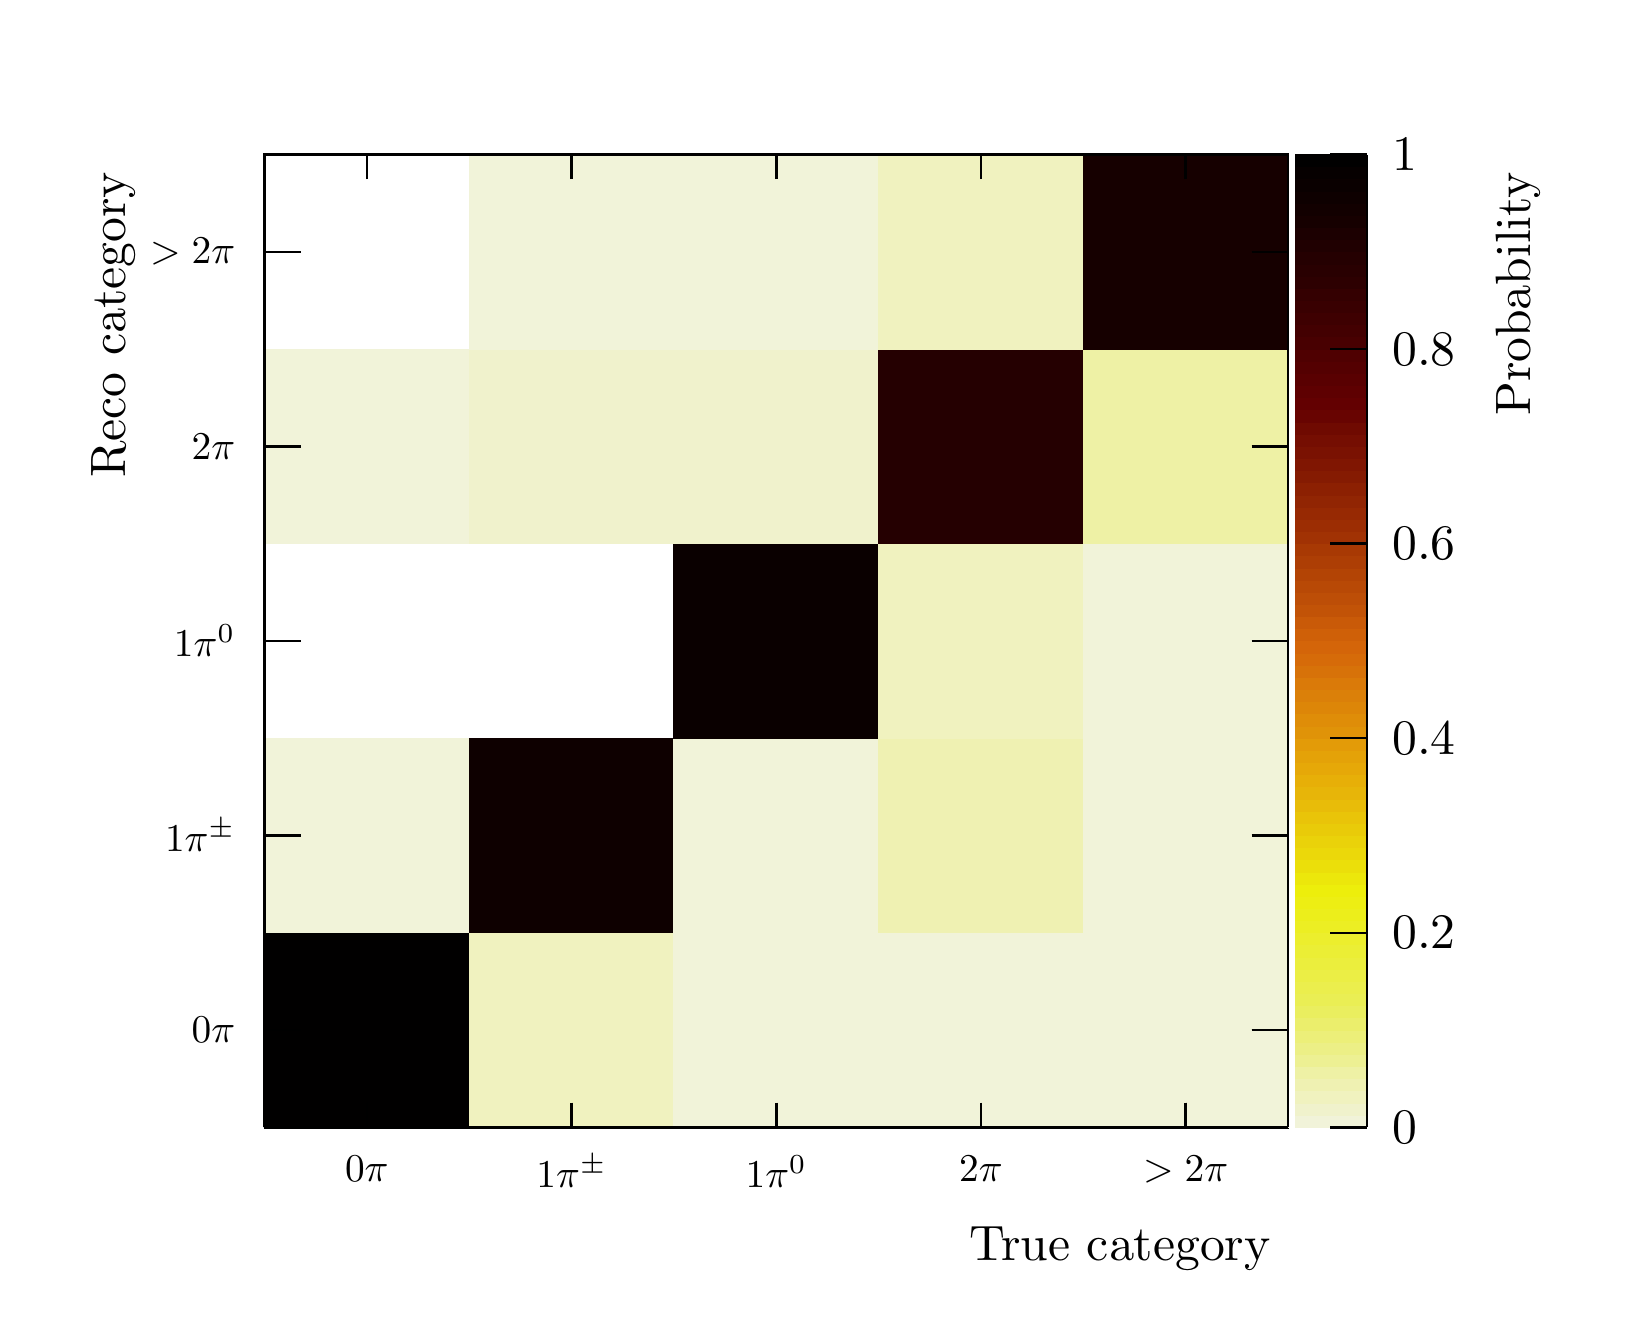
\begin{tikzpicture}
\pgfdeclareplotmark{cross} {
\pgfpathmoveto{\pgfpoint{-0.3\pgfplotmarksize}{\pgfplotmarksize}}
\pgfpathlineto{\pgfpoint{+0.3\pgfplotmarksize}{\pgfplotmarksize}}
\pgfpathlineto{\pgfpoint{+0.3\pgfplotmarksize}{0.3\pgfplotmarksize}}
\pgfpathlineto{\pgfpoint{+1\pgfplotmarksize}{0.3\pgfplotmarksize}}
\pgfpathlineto{\pgfpoint{+1\pgfplotmarksize}{-0.3\pgfplotmarksize}}
\pgfpathlineto{\pgfpoint{+0.3\pgfplotmarksize}{-0.3\pgfplotmarksize}}
\pgfpathlineto{\pgfpoint{+0.3\pgfplotmarksize}{-1.\pgfplotmarksize}}
\pgfpathlineto{\pgfpoint{-0.3\pgfplotmarksize}{-1.\pgfplotmarksize}}
\pgfpathlineto{\pgfpoint{-0.3\pgfplotmarksize}{-0.3\pgfplotmarksize}}
\pgfpathlineto{\pgfpoint{-1.\pgfplotmarksize}{-0.3\pgfplotmarksize}}
\pgfpathlineto{\pgfpoint{-1.\pgfplotmarksize}{0.3\pgfplotmarksize}}
\pgfpathlineto{\pgfpoint{-0.3\pgfplotmarksize}{0.3\pgfplotmarksize}}
\pgfpathclose
\pgfusepathqstroke
}
\pgfdeclareplotmark{cross*} {
\pgfpathmoveto{\pgfpoint{-0.3\pgfplotmarksize}{\pgfplotmarksize}}
\pgfpathlineto{\pgfpoint{+0.3\pgfplotmarksize}{\pgfplotmarksize}}
\pgfpathlineto{\pgfpoint{+0.3\pgfplotmarksize}{0.3\pgfplotmarksize}}
\pgfpathlineto{\pgfpoint{+1\pgfplotmarksize}{0.3\pgfplotmarksize}}
\pgfpathlineto{\pgfpoint{+1\pgfplotmarksize}{-0.3\pgfplotmarksize}}
\pgfpathlineto{\pgfpoint{+0.3\pgfplotmarksize}{-0.3\pgfplotmarksize}}
\pgfpathlineto{\pgfpoint{+0.3\pgfplotmarksize}{-1.\pgfplotmarksize}}
\pgfpathlineto{\pgfpoint{-0.3\pgfplotmarksize}{-1.\pgfplotmarksize}}
\pgfpathlineto{\pgfpoint{-0.3\pgfplotmarksize}{-0.3\pgfplotmarksize}}
\pgfpathlineto{\pgfpoint{-1.\pgfplotmarksize}{-0.3\pgfplotmarksize}}
\pgfpathlineto{\pgfpoint{-1.\pgfplotmarksize}{0.3\pgfplotmarksize}}
\pgfpathlineto{\pgfpoint{-0.3\pgfplotmarksize}{0.3\pgfplotmarksize}}
\pgfpathclose
\pgfusepathqfillstroke
}
\pgfdeclareplotmark{newstar} {
\pgfpathmoveto{\pgfqpoint{0pt}{\pgfplotmarksize}}
\pgfpathlineto{\pgfqpointpolar{44}{0.5\pgfplotmarksize}}
\pgfpathlineto{\pgfqpointpolar{18}{\pgfplotmarksize}}
\pgfpathlineto{\pgfqpointpolar{-20}{0.5\pgfplotmarksize}}
\pgfpathlineto{\pgfqpointpolar{-54}{\pgfplotmarksize}}
\pgfpathlineto{\pgfqpointpolar{-90}{0.5\pgfplotmarksize}}
\pgfpathlineto{\pgfqpointpolar{234}{\pgfplotmarksize}}
\pgfpathlineto{\pgfqpointpolar{198}{0.5\pgfplotmarksize}}
\pgfpathlineto{\pgfqpointpolar{162}{\pgfplotmarksize}}
\pgfpathlineto{\pgfqpointpolar{134}{0.5\pgfplotmarksize}}
\pgfpathclose
\pgfusepathqstroke
}
\pgfdeclareplotmark{newstar*} {
\pgfpathmoveto{\pgfqpoint{0pt}{\pgfplotmarksize}}
\pgfpathlineto{\pgfqpointpolar{44}{0.5\pgfplotmarksize}}
\pgfpathlineto{\pgfqpointpolar{18}{\pgfplotmarksize}}
\pgfpathlineto{\pgfqpointpolar{-20}{0.5\pgfplotmarksize}}
\pgfpathlineto{\pgfqpointpolar{-54}{\pgfplotmarksize}}
\pgfpathlineto{\pgfqpointpolar{-90}{0.5\pgfplotmarksize}}
\pgfpathlineto{\pgfqpointpolar{234}{\pgfplotmarksize}}
\pgfpathlineto{\pgfqpointpolar{198}{0.5\pgfplotmarksize}}
\pgfpathlineto{\pgfqpointpolar{162}{\pgfplotmarksize}}
\pgfpathlineto{\pgfqpointpolar{134}{0.5\pgfplotmarksize}}
\pgfpathclose
\pgfusepathqfillstroke
}
\definecolor{c}{rgb}{1,1,1};
\draw [color=c, fill=c] (0,0) rectangle (20,16.0446);
\draw [color=c, fill=c] (3,2.08579) rectangle (16,14.4401);
\definecolor{c}{rgb}{0,0,0};
\draw [c,line width=0.9] (3,2.08579) -- (3,14.4401) -- (16,14.4401) -- (16,2.08579) -- (3,2.08579);
\definecolor{c}{rgb}{1,1,1};
\draw [color=c, fill=c] (3,2.08579) rectangle (16,14.4401);
\definecolor{c}{rgb}{0,0,0};
\draw [c,line width=0.9] (3,2.08579) -- (3,14.4401) -- (16,14.4401) -- (16,2.08579) -- (3,2.08579);
\definecolor{c}{rgb}{0.00551471,0,0.000122549};
\draw [color=c, fill=c] (3,2.08579) rectangle (5.6,4.55666);
\definecolor{c}{rgb}{0.939911,0.947249,0.748261};
\draw [color=c, fill=c] (5.6,2.08579) rectangle (8.2,4.55666);
\definecolor{c}{rgb}{0.945984,0.951044,0.850727};
\draw [color=c, fill=c] (8.2,2.08579) rectangle (10.8,4.55666);
\draw [color=c, fill=c] (10.8,2.08579) rectangle (13.4,4.55666);
\draw [color=c, fill=c] (13.4,2.08579) rectangle (16,4.55666);
\draw [color=c, fill=c] (3,4.55666) rectangle (5.6,7.02752);
\definecolor{c}{rgb}{0.0551471,0,0.00122549};
\draw [color=c, fill=c] (5.6,4.55666) rectangle (8.2,7.02752);
\definecolor{c}{rgb}{0.945984,0.951044,0.850727};
\draw [color=c, fill=c] (8.2,4.55666) rectangle (10.8,7.02752);
\definecolor{c}{rgb}{0.936875,0.945351,0.697027};
\draw [color=c, fill=c] (10.8,4.55666) rectangle (13.4,7.02752);
\definecolor{c}{rgb}{0.945984,0.951044,0.850727};
\draw [color=c, fill=c] (13.4,4.55666) rectangle (16,7.02752);
\definecolor{c}{rgb}{0.0386029,0,0.000857843};
\draw [color=c, fill=c] (8.2,7.02752) rectangle (10.8,9.49838);
\definecolor{c}{rgb}{0.939911,0.947249,0.748261};
\draw [color=c, fill=c] (10.8,7.02752) rectangle (13.4,9.49838);
\definecolor{c}{rgb}{0.945984,0.951044,0.850727};
\draw [color=c, fill=c] (13.4,7.02752) rectangle (16,9.49838);
\draw [color=c, fill=c] (3,9.49838) rectangle (5.6,11.9692);
\definecolor{c}{rgb}{0.942948,0.949146,0.799494};
\draw [color=c, fill=c] (5.6,9.49838) rectangle (8.2,11.9692);
\draw [color=c, fill=c] (8.2,9.49838) rectangle (10.8,11.9692);
\definecolor{c}{rgb}{0.143382,0,0.00318627};
\draw [color=c, fill=c] (10.8,9.49838) rectangle (13.4,11.9692);
\definecolor{c}{rgb}{0.933839,0.943453,0.645794};
\draw [color=c, fill=c] (13.4,9.49838) rectangle (16,11.9692);
\definecolor{c}{rgb}{0.945984,0.951044,0.850727};
\draw [color=c, fill=c] (5.6,11.9692) rectangle (8.2,14.4401);
\draw [color=c, fill=c] (8.2,11.9692) rectangle (10.8,14.4401);
\definecolor{c}{rgb}{0.939911,0.947249,0.748261};
\draw [color=c, fill=c] (10.8,11.9692) rectangle (13.4,14.4401);
\definecolor{c}{rgb}{0.0882353,0,0.00196078};
\draw [color=c, fill=c] (13.4,11.9692) rectangle (16,14.4401);
\definecolor{c}{rgb}{0,0,0};
\draw [c,line width=0.9] (3,2.08579) -- (16,2.08579);
\draw [anchor=north] (4.3,1.90048) node[scale=1.42291, color=c, rotate=0]{$0\pi$};
\draw [anchor=north] (6.9,1.90048) node[scale=1.42291, color=c, rotate=0]{$1\pi^{\pm}$};
\draw [anchor=north] (9.5,1.90048) node[scale=1.42291, color=c, rotate=0]{$1\pi^{0}$};
\draw [anchor=north] (12.1,1.90048) node[scale=1.42291, color=c, rotate=0]{$2\pi$};
\draw [anchor=north] (14.7,1.90048) node[scale=1.42291, color=c, rotate=0]{$>2\pi$};
\draw [c,line width=0.9] (4.3,2.39866) -- (4.3,2.08579);
\draw [c,line width=0.9] (6.9,2.39866) -- (6.9,2.08579);
\draw [c,line width=0.9] (9.5,2.39866) -- (9.5,2.08579);
\draw [c,line width=0.9] (12.1,2.39866) -- (12.1,2.08579);
\draw [c,line width=0.9] (14.7,2.39866) -- (14.7,2.08579);
\draw [c,line width=0.9] (4.3,2.39866) -- (4.3,2.08579);
\draw [c,line width=0.9] (14.7,2.39866) -- (14.7,2.08579);
\draw [anchor= east] (16,0.545515) node[scale=1.7941, color=c, rotate=0]{ True category};
\draw [c,line width=0.9] (3,14.4401) -- (16,14.4401);
\draw [c,line width=0.9] (4.3,14.1272) -- (4.3,14.4401);
\draw [c,line width=0.9] (6.9,14.1272) -- (6.9,14.4401);
\draw [c,line width=0.9] (9.5,14.1272) -- (9.5,14.4401);
\draw [c,line width=0.9] (12.1,14.1272) -- (12.1,14.4401);
\draw [c,line width=0.9] (14.7,14.1272) -- (14.7,14.4401);
\draw [c,line width=0.9] (4.3,14.1272) -- (4.3,14.4401);
\draw [c,line width=0.9] (14.7,14.1272) -- (14.7,14.4401);
\draw [c,line width=0.9] (3,2.08579) -- (3,14.4401);
\draw [anchor= east] (2.805,3.32123) node[scale=1.42291, color=c, rotate=0]{$0\pi$};
\draw [anchor= east] (2.805,5.79209) node[scale=1.42291, color=c, rotate=0]{$1\pi^{\pm}$};
\draw [anchor= east] (2.805,8.26295) node[scale=1.42291, color=c, rotate=0]{$1\pi^{0}$};
\draw [anchor= east] (2.805,10.7338) node[scale=1.42291, color=c, rotate=0]{$2\pi$};
\draw [anchor= east] (2.805,13.2047) node[scale=1.42291, color=c, rotate=0]{$>2\pi$};
\draw [c,line width=0.9] (3.462,3.32123) -- (3,3.32123);
\draw [c,line width=0.9] (3.462,5.79209) -- (3,5.79209);
\draw [c,line width=0.9] (3.462,8.26295) -- (3,8.26295);
\draw [c,line width=0.9] (3.462,10.7338) -- (3,10.7338);
\draw [c,line width=0.9] (3.462,13.2047) -- (3,13.2047);
\draw [c,line width=0.9] (3.462,3.32123) -- (3,3.32123);
\draw [c,line width=0.9] (3.462,13.2047) -- (3,13.2047);
\draw [anchor= east] (1.08,14.4401) node[scale=1.7941, color=c, rotate=90]{ Reco category};
\draw [c,line width=0.9] (16,2.08579) -- (16,14.4401);
\draw [c,line width=0.9] (15.538,3.32123) -- (16,3.32123);
\draw [c,line width=0.9] (15.538,5.79209) -- (16,5.79209);
\draw [c,line width=0.9] (15.538,8.26295) -- (16,8.26295);
\draw [c,line width=0.9] (15.538,10.7338) -- (16,10.7338);
\draw [c,line width=0.9] (15.538,13.2047) -- (16,13.2047);
\draw [c,line width=0.9] (15.538,3.32123) -- (16,3.32123);
\draw [c,line width=0.9] (15.538,13.2047) -- (16,13.2047);
\definecolor{c}{rgb}{0.945984,0.951044,0.850727};
\draw [color=c, fill=c] (16.1,2.08579) rectangle (17,2.24022);
\definecolor{c}{rgb}{0.942948,0.949146,0.799494};
\draw [color=c, fill=c] (16.1,2.24022) rectangle (17,2.39465);
\definecolor{c}{rgb}{0.939911,0.947249,0.748261};
\draw [color=c, fill=c] (16.1,2.39465) rectangle (17,2.54908);
\definecolor{c}{rgb}{0.936875,0.945351,0.697027};
\draw [color=c, fill=c] (16.1,2.54908) rectangle (17,2.70351);
\definecolor{c}{rgb}{0.933839,0.943453,0.645794};
\draw [color=c, fill=c] (16.1,2.70351) rectangle (17,2.85794);
\definecolor{c}{rgb}{0.929791,0.940923,0.577483};
\draw [color=c, fill=c] (16.1,2.85794) rectangle (17,3.01237);
\definecolor{c}{rgb}{0.926755,0.939026,0.526249};
\draw [color=c, fill=c] (16.1,3.01237) rectangle (17,3.1668);
\definecolor{c}{rgb}{0.923719,0.937128,0.475016};
\draw [color=c, fill=c] (16.1,3.1668) rectangle (17,3.32123);
\definecolor{c}{rgb}{0.920683,0.935231,0.423782};
\draw [color=c, fill=c] (16.1,3.32123) rectangle (17,3.47565);
\definecolor{c}{rgb}{0.917647,0.933333,0.372549};
\draw [color=c, fill=c] (16.1,3.47565) rectangle (17,3.63008);
\definecolor{c}{rgb}{0.919118,0.933333,0.331373};
\draw [color=c, fill=c] (16.1,3.63008) rectangle (17,3.78451);
\definecolor{c}{rgb}{0.920221,0.933333,0.30049};
\draw [color=c, fill=c] (16.1,3.78451) rectangle (17,3.93894);
\definecolor{c}{rgb}{0.921324,0.933333,0.269608};
\draw [color=c, fill=c] (16.1,3.93894) rectangle (17,4.09337);
\definecolor{c}{rgb}{0.922426,0.933333,0.238725};
\draw [color=c, fill=c] (16.1,4.09337) rectangle (17,4.2478);
\definecolor{c}{rgb}{0.923529,0.933333,0.207843};
\draw [color=c, fill=c] (16.1,4.2478) rectangle (17,4.40223);
\definecolor{c}{rgb}{0.924632,0.933333,0.176961};
\draw [color=c, fill=c] (16.1,4.40223) rectangle (17,4.55666);
\definecolor{c}{rgb}{0.926103,0.933333,0.135784};
\draw [color=c, fill=c] (16.1,4.55666) rectangle (17,4.71109);
\definecolor{c}{rgb}{0.927206,0.933333,0.104902};
\draw [color=c, fill=c] (16.1,4.71109) rectangle (17,4.86552);
\definecolor{c}{rgb}{0.928309,0.933333,0.0740196};
\draw [color=c, fill=c] (16.1,4.86552) rectangle (17,5.01994);
\definecolor{c}{rgb}{0.929412,0.933333,0.0431373};
\draw [color=c, fill=c] (16.1,5.01994) rectangle (17,5.17437);
\definecolor{c}{rgb}{0.926838,0.907598,0.0420343};
\draw [color=c, fill=c] (16.1,5.17437) rectangle (17,5.3288);
\definecolor{c}{rgb}{0.923407,0.873284,0.0405637};
\draw [color=c, fill=c] (16.1,5.3288) rectangle (17,5.48323);
\definecolor{c}{rgb}{0.920833,0.847549,0.0394608};
\draw [color=c, fill=c] (16.1,5.48323) rectangle (17,5.63766);
\definecolor{c}{rgb}{0.91826,0.821814,0.0383578};
\draw [color=c, fill=c] (16.1,5.63766) rectangle (17,5.79209);
\definecolor{c}{rgb}{0.915686,0.796078,0.0372549};
\draw [color=c, fill=c] (16.1,5.79209) rectangle (17,5.94652);
\definecolor{c}{rgb}{0.913113,0.770343,0.036152};
\draw [color=c, fill=c] (16.1,5.94652) rectangle (17,6.10095);
\definecolor{c}{rgb}{0.909681,0.736029,0.0346814};
\draw [color=c, fill=c] (16.1,6.10095) rectangle (17,6.25538);
\definecolor{c}{rgb}{0.907108,0.710294,0.0335784};
\draw [color=c, fill=c] (16.1,6.25538) rectangle (17,6.40981);
\definecolor{c}{rgb}{0.904534,0.684559,0.0324755};
\draw [color=c, fill=c] (16.1,6.40981) rectangle (17,6.56423);
\definecolor{c}{rgb}{0.901961,0.658824,0.0313726};
\draw [color=c, fill=c] (16.1,6.56423) rectangle (17,6.71866);
\definecolor{c}{rgb}{0.895343,0.634191,0.0317402};
\draw [color=c, fill=c] (16.1,6.71866) rectangle (17,6.87309);
\definecolor{c}{rgb}{0.888726,0.609559,0.0321078};
\draw [color=c, fill=c] (16.1,6.87309) rectangle (17,7.02752);
\definecolor{c}{rgb}{0.879902,0.576716,0.032598};
\draw [color=c, fill=c] (16.1,7.02752) rectangle (17,7.18195);
\definecolor{c}{rgb}{0.873284,0.552083,0.0329657};
\draw [color=c, fill=c] (16.1,7.18195) rectangle (17,7.33638);
\definecolor{c}{rgb}{0.866667,0.527451,0.0333333};
\draw [color=c, fill=c] (16.1,7.33638) rectangle (17,7.49081);
\definecolor{c}{rgb}{0.860049,0.502819,0.033701};
\draw [color=c, fill=c] (16.1,7.49081) rectangle (17,7.64524);
\definecolor{c}{rgb}{0.853431,0.478186,0.0340686};
\draw [color=c, fill=c] (16.1,7.64524) rectangle (17,7.79967);
\definecolor{c}{rgb}{0.844608,0.445343,0.0345588};
\draw [color=c, fill=c] (16.1,7.79967) rectangle (17,7.95409);
\definecolor{c}{rgb}{0.83799,0.420711,0.0349265};
\draw [color=c, fill=c] (16.1,7.95409) rectangle (17,8.10852);
\definecolor{c}{rgb}{0.831373,0.396078,0.0352941};
\draw [color=c, fill=c] (16.1,8.10852) rectangle (17,8.26295);
\definecolor{c}{rgb}{0.810784,0.37549,0.0330882};
\draw [color=c, fill=c] (16.1,8.26295) rectangle (17,8.41738);
\definecolor{c}{rgb}{0.790196,0.354902,0.0308824};
\draw [color=c, fill=c] (16.1,8.41738) rectangle (17,8.57181);
\definecolor{c}{rgb}{0.762745,0.327451,0.0279412};
\draw [color=c, fill=c] (16.1,8.57181) rectangle (17,8.72624);
\definecolor{c}{rgb}{0.742157,0.306863,0.0257353};
\draw [color=c, fill=c] (16.1,8.72624) rectangle (17,8.88067);
\definecolor{c}{rgb}{0.721569,0.286275,0.0235294};
\draw [color=c, fill=c] (16.1,8.88067) rectangle (17,9.0351);
\definecolor{c}{rgb}{0.70098,0.265686,0.0213235};
\draw [color=c, fill=c] (16.1,9.0351) rectangle (17,9.18953);
\definecolor{c}{rgb}{0.680392,0.245098,0.0191176};
\draw [color=c, fill=c] (16.1,9.18953) rectangle (17,9.34396);
\definecolor{c}{rgb}{0.659804,0.22451,0.0169118};
\draw [color=c, fill=c] (16.1,9.34396) rectangle (17,9.49838);
\definecolor{c}{rgb}{0.632353,0.197059,0.0139706};
\draw [color=c, fill=c] (16.1,9.49838) rectangle (17,9.65281);
\definecolor{c}{rgb}{0.611765,0.176471,0.0117647};
\draw [color=c, fill=c] (16.1,9.65281) rectangle (17,9.80724);
\definecolor{c}{rgb}{0.590809,0.159926,0.0110294};
\draw [color=c, fill=c] (16.1,9.80724) rectangle (17,9.96167);
\definecolor{c}{rgb}{0.569853,0.143382,0.0102941};
\draw [color=c, fill=c] (16.1,9.96167) rectangle (17,10.1161);
\definecolor{c}{rgb}{0.548897,0.126838,0.00955882};
\draw [color=c, fill=c] (16.1,10.1161) rectangle (17,10.2705);
\definecolor{c}{rgb}{0.520956,0.104779,0.00857843};
\draw [color=c, fill=c] (16.1,10.2705) rectangle (17,10.425);
\definecolor{c}{rgb}{0.5,0.0882353,0.00784314};
\draw [color=c, fill=c] (16.1,10.425) rectangle (17,10.5794);
\definecolor{c}{rgb}{0.479044,0.0716912,0.00710784};
\draw [color=c, fill=c] (16.1,10.5794) rectangle (17,10.7338);
\definecolor{c}{rgb}{0.458088,0.0551471,0.00637255};
\draw [color=c, fill=c] (16.1,10.7338) rectangle (17,10.8882);
\definecolor{c}{rgb}{0.437132,0.0386029,0.00563726};
\draw [color=c, fill=c] (16.1,10.8882) rectangle (17,11.0427);
\definecolor{c}{rgb}{0.409191,0.0165441,0.00465686};
\draw [color=c, fill=c] (16.1,11.0427) rectangle (17,11.1971);
\definecolor{c}{rgb}{0.388235,0,0.00392157};
\draw [color=c, fill=c] (16.1,11.1971) rectangle (17,11.3515);
\definecolor{c}{rgb}{0.368382,0,0.00392157};
\draw [color=c, fill=c] (16.1,11.3515) rectangle (17,11.506);
\definecolor{c}{rgb}{0.348529,0,0.00392157};
\draw [color=c, fill=c] (16.1,11.506) rectangle (17,11.6604);
\definecolor{c}{rgb}{0.328676,0,0.00392157};
\draw [color=c, fill=c] (16.1,11.6604) rectangle (17,11.8148);
\definecolor{c}{rgb}{0.308824,0,0.00392157};
\draw [color=c, fill=c] (16.1,11.8148) rectangle (17,11.9692);
\definecolor{c}{rgb}{0.282353,0,0.00392157};
\draw [color=c, fill=c] (16.1,11.9692) rectangle (17,12.1237);
\definecolor{c}{rgb}{0.2625,0,0.00392157};
\draw [color=c, fill=c] (16.1,12.1237) rectangle (17,12.2781);
\definecolor{c}{rgb}{0.242647,0,0.00392157};
\draw [color=c, fill=c] (16.1,12.2781) rectangle (17,12.4325);
\definecolor{c}{rgb}{0.222794,0,0.00392157};
\draw [color=c, fill=c] (16.1,12.4325) rectangle (17,12.587);
\definecolor{c}{rgb}{0.202941,0,0.00392157};
\draw [color=c, fill=c] (16.1,12.587) rectangle (17,12.7414);
\definecolor{c}{rgb}{0.176471,0,0.00392157};
\draw [color=c, fill=c] (16.1,12.7414) rectangle (17,12.8958);
\definecolor{c}{rgb}{0.159926,0,0.00355392};
\draw [color=c, fill=c] (16.1,12.8958) rectangle (17,13.0503);
\definecolor{c}{rgb}{0.143382,0,0.00318627};
\draw [color=c, fill=c] (16.1,13.0503) rectangle (17,13.2047);
\definecolor{c}{rgb}{0.126838,0,0.00281863};
\draw [color=c, fill=c] (16.1,13.2047) rectangle (17,13.3591);
\definecolor{c}{rgb}{0.110294,0,0.00245098};
\draw [color=c, fill=c] (16.1,13.3591) rectangle (17,13.5135);
\definecolor{c}{rgb}{0.0882353,0,0.00196078};
\draw [color=c, fill=c] (16.1,13.5135) rectangle (17,13.668);
\definecolor{c}{rgb}{0.0716912,0,0.00159314};
\draw [color=c, fill=c] (16.1,13.668) rectangle (17,13.8224);
\definecolor{c}{rgb}{0.0551471,0,0.00122549};
\draw [color=c, fill=c] (16.1,13.8224) rectangle (17,13.9768);
\definecolor{c}{rgb}{0.0386029,0,0.000857843};
\draw [color=c, fill=c] (16.1,13.9768) rectangle (17,14.1313);
\definecolor{c}{rgb}{0.0220588,0,0.000490196};
\draw [color=c, fill=c] (16.1,14.1313) rectangle (17,14.2857);
\definecolor{c}{rgb}{0.00551471,0,0.000122549};
\draw [color=c, fill=c] (16.1,14.2857) rectangle (17,14.4401);
\definecolor{c}{rgb}{0,0,0};
\draw [c,line width=0.9] (17,2.08579) -- (17,14.4401);
\draw [c,line width=0.9] (16.538,2.08579) -- (17,2.08579);
\draw [c,line width=0.9] (16.538,4.55666) -- (17,4.55666);
\draw [c,line width=0.9] (16.538,7.02752) -- (17,7.02752);
\draw [c,line width=0.9] (16.538,9.49838) -- (17,9.49838);
\draw [c,line width=0.9] (16.538,11.9692) -- (17,11.9692);
\draw [c,line width=0.9] (16.538,14.4401) -- (17,14.4401);
\draw [c,line width=0.9] (16.538,14.4401) -- (17,14.4401);
\draw [anchor= west] (17.1,2.08579) node[scale=1.7941, color=c, rotate=0]{0};
\draw [anchor= west] (17.1,4.55666) node[scale=1.7941, color=c, rotate=0]{0.2};
\draw [anchor= west] (17.1,7.02752) node[scale=1.7941, color=c, rotate=0]{0.4};
\draw [anchor= west] (17.1,9.49838) node[scale=1.7941, color=c, rotate=0]{0.6};
\draw [anchor= west] (17.1,11.9692) node[scale=1.7941, color=c, rotate=0]{0.8};
\draw [anchor= west] (17.1,14.4401) node[scale=1.7941, color=c, rotate=0]{1};
\draw [anchor= east] (18.92,14.4401) node[scale=1.7941, color=c, rotate=90]{ Probability};
\definecolor{c}{rgb}{1,1,1};
\draw [color=c, fill=c] (2,15.0819) rectangle (18,15.9643);
\definecolor{c}{rgb}{0,0,0};
%\draw (10,15.5231) node[scale=1.67037, color=c, rotate=0]{Final state confusion matrix in HPgTPC};
\end{tikzpicture}

		\end{adjustbox}
	\end{minipage}
	\caption[Confusion matrices for final state pion multiplicities in ND-GAr]{Left: Confusion matrix for final state pion multiplicities in ND-GAr with the neutrino beam in FHC mode. Right: Confusion matrix for final state pion multiplicities in ND-GAr with the neutrino beam in RHC mode.}
	\label{fig:confusMatPi}
\end{figure}

%\begin{figure}[h]
%	\begin{minipage}[t]{.49\linewidth}
%		\begin{adjustbox}{max totalsize=\linewidth, center}
%			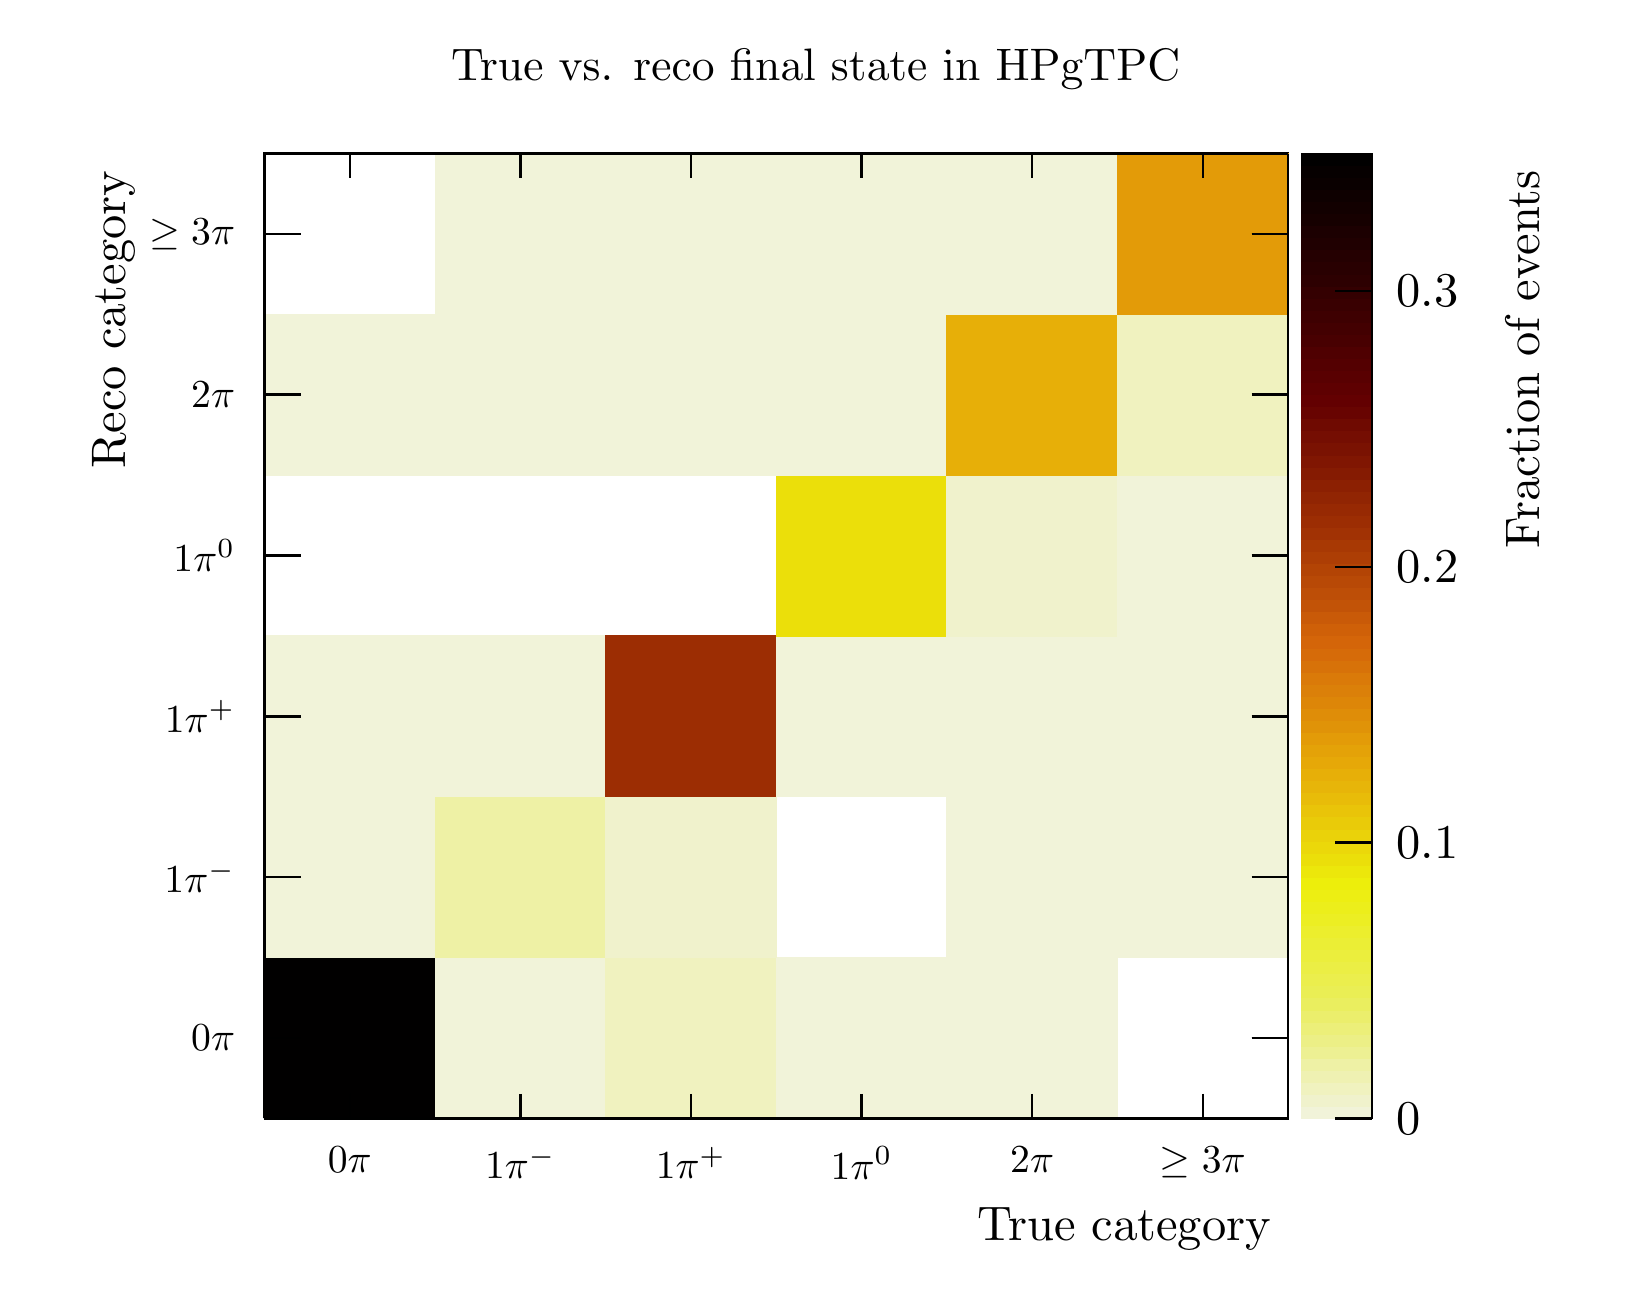
\begin{tikzpicture}
\pgfdeclareplotmark{cross} {
\pgfpathmoveto{\pgfpoint{-0.3\pgfplotmarksize}{\pgfplotmarksize}}
\pgfpathlineto{\pgfpoint{+0.3\pgfplotmarksize}{\pgfplotmarksize}}
\pgfpathlineto{\pgfpoint{+0.3\pgfplotmarksize}{0.3\pgfplotmarksize}}
\pgfpathlineto{\pgfpoint{+1\pgfplotmarksize}{0.3\pgfplotmarksize}}
\pgfpathlineto{\pgfpoint{+1\pgfplotmarksize}{-0.3\pgfplotmarksize}}
\pgfpathlineto{\pgfpoint{+0.3\pgfplotmarksize}{-0.3\pgfplotmarksize}}
\pgfpathlineto{\pgfpoint{+0.3\pgfplotmarksize}{-1.\pgfplotmarksize}}
\pgfpathlineto{\pgfpoint{-0.3\pgfplotmarksize}{-1.\pgfplotmarksize}}
\pgfpathlineto{\pgfpoint{-0.3\pgfplotmarksize}{-0.3\pgfplotmarksize}}
\pgfpathlineto{\pgfpoint{-1.\pgfplotmarksize}{-0.3\pgfplotmarksize}}
\pgfpathlineto{\pgfpoint{-1.\pgfplotmarksize}{0.3\pgfplotmarksize}}
\pgfpathlineto{\pgfpoint{-0.3\pgfplotmarksize}{0.3\pgfplotmarksize}}
\pgfpathclose
\pgfusepathqstroke
}
\pgfdeclareplotmark{cross*} {
\pgfpathmoveto{\pgfpoint{-0.3\pgfplotmarksize}{\pgfplotmarksize}}
\pgfpathlineto{\pgfpoint{+0.3\pgfplotmarksize}{\pgfplotmarksize}}
\pgfpathlineto{\pgfpoint{+0.3\pgfplotmarksize}{0.3\pgfplotmarksize}}
\pgfpathlineto{\pgfpoint{+1\pgfplotmarksize}{0.3\pgfplotmarksize}}
\pgfpathlineto{\pgfpoint{+1\pgfplotmarksize}{-0.3\pgfplotmarksize}}
\pgfpathlineto{\pgfpoint{+0.3\pgfplotmarksize}{-0.3\pgfplotmarksize}}
\pgfpathlineto{\pgfpoint{+0.3\pgfplotmarksize}{-1.\pgfplotmarksize}}
\pgfpathlineto{\pgfpoint{-0.3\pgfplotmarksize}{-1.\pgfplotmarksize}}
\pgfpathlineto{\pgfpoint{-0.3\pgfplotmarksize}{-0.3\pgfplotmarksize}}
\pgfpathlineto{\pgfpoint{-1.\pgfplotmarksize}{-0.3\pgfplotmarksize}}
\pgfpathlineto{\pgfpoint{-1.\pgfplotmarksize}{0.3\pgfplotmarksize}}
\pgfpathlineto{\pgfpoint{-0.3\pgfplotmarksize}{0.3\pgfplotmarksize}}
\pgfpathclose
\pgfusepathqfillstroke
}
\pgfdeclareplotmark{newstar} {
\pgfpathmoveto{\pgfqpoint{0pt}{\pgfplotmarksize}}
\pgfpathlineto{\pgfqpointpolar{44}{0.5\pgfplotmarksize}}
\pgfpathlineto{\pgfqpointpolar{18}{\pgfplotmarksize}}
\pgfpathlineto{\pgfqpointpolar{-20}{0.5\pgfplotmarksize}}
\pgfpathlineto{\pgfqpointpolar{-54}{\pgfplotmarksize}}
\pgfpathlineto{\pgfqpointpolar{-90}{0.5\pgfplotmarksize}}
\pgfpathlineto{\pgfqpointpolar{234}{\pgfplotmarksize}}
\pgfpathlineto{\pgfqpointpolar{198}{0.5\pgfplotmarksize}}
\pgfpathlineto{\pgfqpointpolar{162}{\pgfplotmarksize}}
\pgfpathlineto{\pgfqpointpolar{134}{0.5\pgfplotmarksize}}
\pgfpathclose
\pgfusepathqstroke
}
\pgfdeclareplotmark{newstar*} {
\pgfpathmoveto{\pgfqpoint{0pt}{\pgfplotmarksize}}
\pgfpathlineto{\pgfqpointpolar{44}{0.5\pgfplotmarksize}}
\pgfpathlineto{\pgfqpointpolar{18}{\pgfplotmarksize}}
\pgfpathlineto{\pgfqpointpolar{-20}{0.5\pgfplotmarksize}}
\pgfpathlineto{\pgfqpointpolar{-54}{\pgfplotmarksize}}
\pgfpathlineto{\pgfqpointpolar{-90}{0.5\pgfplotmarksize}}
\pgfpathlineto{\pgfqpointpolar{234}{\pgfplotmarksize}}
\pgfpathlineto{\pgfqpointpolar{198}{0.5\pgfplotmarksize}}
\pgfpathlineto{\pgfqpointpolar{162}{\pgfplotmarksize}}
\pgfpathlineto{\pgfqpointpolar{134}{0.5\pgfplotmarksize}}
\pgfpathclose
\pgfusepathqfillstroke
}
\definecolor{c}{rgb}{1,1,1};
\draw [color=c, fill=c] (0,0) rectangle (20,15.914);
\draw [color=c, fill=c] (3,2.06882) rectangle (16,14.3226);
\definecolor{c}{rgb}{0,0,0};
\draw [c,line width=0.9] (3,2.06882) -- (3,14.3226) -- (16,14.3226) -- (16,2.06882) -- (3,2.06882);
\definecolor{c}{rgb}{1,1,1};
\draw [color=c, fill=c] (3,2.06882) rectangle (16,14.3226);
\definecolor{c}{rgb}{0,0,0};
\draw [c,line width=0.9] (3,2.06882) -- (3,14.3226) -- (16,14.3226) -- (16,2.06882) -- (3,2.06882);
\definecolor{c}{rgb}{0.00551471,0,0.000122549};
\draw [color=c, fill=c] (3,2.06882) rectangle (5.16667,4.11111);
\definecolor{c}{rgb}{0.945984,0.951044,0.850727};
\draw [color=c, fill=c] (5.16667,2.06882) rectangle (7.33333,4.11111);
\definecolor{c}{rgb}{0.939911,0.947249,0.748261};
\draw [color=c, fill=c] (7.33333,2.06882) rectangle (9.5,4.11111);
\definecolor{c}{rgb}{0.945984,0.951044,0.850727};
\draw [color=c, fill=c] (9.5,2.06882) rectangle (11.6667,4.11111);
\draw [color=c, fill=c] (11.6667,2.06882) rectangle (13.8333,4.11111);
\draw [color=c, fill=c] (3,4.11111) rectangle (5.16667,6.15341);
\definecolor{c}{rgb}{0.933839,0.943453,0.645794};
\draw [color=c, fill=c] (5.16667,4.11111) rectangle (7.33333,6.15341);
\definecolor{c}{rgb}{0.942948,0.949146,0.799494};
\draw [color=c, fill=c] (7.33333,4.11111) rectangle (9.5,6.15341);
\definecolor{c}{rgb}{0.945984,0.951044,0.850727};
\draw [color=c, fill=c] (11.6667,4.11111) rectangle (13.8333,6.15341);
\draw [color=c, fill=c] (13.8333,4.11111) rectangle (16,6.15341);
\draw [color=c, fill=c] (3,6.15341) rectangle (5.16667,8.1957);
\draw [color=c, fill=c] (5.16667,6.15341) rectangle (7.33333,8.1957);
\definecolor{c}{rgb}{0.611765,0.176471,0.0117647};
\draw [color=c, fill=c] (7.33333,6.15341) rectangle (9.5,8.1957);
\definecolor{c}{rgb}{0.945984,0.951044,0.850727};
\draw [color=c, fill=c] (9.5,6.15341) rectangle (11.6667,8.1957);
\draw [color=c, fill=c] (11.6667,6.15341) rectangle (13.8333,8.1957);
\draw [color=c, fill=c] (13.8333,6.15341) rectangle (16,8.1957);
\definecolor{c}{rgb}{0.923407,0.873284,0.0405637};
\draw [color=c, fill=c] (9.5,8.1957) rectangle (11.6667,10.238);
\definecolor{c}{rgb}{0.942948,0.949146,0.799494};
\draw [color=c, fill=c] (11.6667,8.1957) rectangle (13.8333,10.238);
\definecolor{c}{rgb}{0.945984,0.951044,0.850727};
\draw [color=c, fill=c] (13.8333,8.1957) rectangle (16,10.238);
\draw [color=c, fill=c] (3,10.238) rectangle (5.16667,12.2803);
\draw [color=c, fill=c] (5.16667,10.238) rectangle (7.33333,12.2803);
\draw [color=c, fill=c] (7.33333,10.238) rectangle (9.5,12.2803);
\draw [color=c, fill=c] (9.5,10.238) rectangle (11.6667,12.2803);
\definecolor{c}{rgb}{0.904534,0.684559,0.0324755};
\draw [color=c, fill=c] (11.6667,10.238) rectangle (13.8333,12.2803);
\definecolor{c}{rgb}{0.939911,0.947249,0.748261};
\draw [color=c, fill=c] (13.8333,10.238) rectangle (16,12.2803);
\definecolor{c}{rgb}{0.945984,0.951044,0.850727};
\draw [color=c, fill=c] (5.16667,12.2803) rectangle (7.33333,14.3226);
\draw [color=c, fill=c] (7.33333,12.2803) rectangle (9.5,14.3226);
\draw [color=c, fill=c] (9.5,12.2803) rectangle (11.6667,14.3226);
\draw [color=c, fill=c] (11.6667,12.2803) rectangle (13.8333,14.3226);
\definecolor{c}{rgb}{0.888726,0.609559,0.0321078};
\draw [color=c, fill=c] (13.8333,12.2803) rectangle (16,14.3226);
\definecolor{c}{rgb}{0,0,0};
\draw [c,line width=0.9] (3,2.06882) -- (16,2.06882);
\draw [anchor=north] (4.08333,1.88501) node[scale=1.43288, color=c, rotate=0]{$0\pi$};
\draw [anchor=north] (6.25,1.88501) node[scale=1.43288, color=c, rotate=0]{$1\pi^{-}$};
\draw [anchor=north] (8.41667,1.88501) node[scale=1.43288, color=c, rotate=0]{$1\pi^{+}$};
\draw [anchor=north] (10.5833,1.88501) node[scale=1.43288, color=c, rotate=0]{$1\pi^{0}$};
\draw [anchor=north] (12.75,1.88501) node[scale=1.43288, color=c, rotate=0]{$2\pi$};
\draw [anchor=north] (14.9167,1.88501) node[scale=1.43288, color=c, rotate=0]{$\geq3\pi$};
\draw [c,line width=0.9] (4.08333,2.37914) -- (4.08333,2.06882);
\draw [c,line width=0.9] (6.25,2.37914) -- (6.25,2.06882);
\draw [c,line width=0.9] (8.41667,2.37914) -- (8.41667,2.06882);
\draw [c,line width=0.9] (10.5833,2.37914) -- (10.5833,2.06882);
\draw [c,line width=0.9] (12.75,2.37914) -- (12.75,2.06882);
\draw [c,line width=0.9] (14.9167,2.37914) -- (14.9167,2.06882);
\draw [c,line width=0.9] (4.08333,2.37914) -- (4.08333,2.06882);
\draw [c,line width=0.9] (14.9167,2.37914) -- (14.9167,2.06882);
\draw [anchor= east] (16,0.668387) node[scale=1.7513, color=c, rotate=0]{ True category};
\draw [c,line width=0.9] (3,14.3226) -- (16,14.3226);
\draw [c,line width=0.9] (4.08333,14.0123) -- (4.08333,14.3226);
\draw [c,line width=0.9] (6.25,14.0123) -- (6.25,14.3226);
\draw [c,line width=0.9] (8.41667,14.0123) -- (8.41667,14.3226);
\draw [c,line width=0.9] (10.5833,14.0123) -- (10.5833,14.3226);
\draw [c,line width=0.9] (12.75,14.0123) -- (12.75,14.3226);
\draw [c,line width=0.9] (14.9167,14.0123) -- (14.9167,14.3226);
\draw [c,line width=0.9] (4.08333,14.0123) -- (4.08333,14.3226);
\draw [c,line width=0.9] (14.9167,14.0123) -- (14.9167,14.3226);
\draw [c,line width=0.9] (3,2.06882) -- (3,14.3226);
\draw [anchor= east] (2.805,3.08996) node[scale=1.43288, color=c, rotate=0]{$0\pi$};
\draw [anchor= east] (2.805,5.13226) node[scale=1.43288, color=c, rotate=0]{$1\pi^{-}$};
\draw [anchor= east] (2.805,7.17455) node[scale=1.43288, color=c, rotate=0]{$1\pi^{+}$};
\draw [anchor= east] (2.805,9.21685) node[scale=1.43288, color=c, rotate=0]{$1\pi^{0}$};
\draw [anchor= east] (2.805,11.2591) node[scale=1.43288, color=c, rotate=0]{$2\pi$};
\draw [anchor= east] (2.805,13.3014) node[scale=1.43288, color=c, rotate=0]{$\geq3\pi$};
\draw [c,line width=0.9] (3.462,3.08996) -- (3,3.08996);
\draw [c,line width=0.9] (3.462,5.13226) -- (3,5.13226);
\draw [c,line width=0.9] (3.462,7.17455) -- (3,7.17455);
\draw [c,line width=0.9] (3.462,9.21685) -- (3,9.21685);
\draw [c,line width=0.9] (3.462,11.2591) -- (3,11.2591);
\draw [c,line width=0.9] (3.462,13.3014) -- (3,13.3014);
\draw [c,line width=0.9] (3.462,3.08996) -- (3,3.08996);
\draw [c,line width=0.9] (3.462,13.3014) -- (3,13.3014);
\draw [anchor= east] (1.08,14.3226) node[scale=1.7513, color=c, rotate=90]{ Reco category};
\draw [c,line width=0.9] (16,2.06882) -- (16,14.3226);
\draw [c,line width=0.9] (15.538,3.08996) -- (16,3.08996);
\draw [c,line width=0.9] (15.538,5.13226) -- (16,5.13226);
\draw [c,line width=0.9] (15.538,7.17455) -- (16,7.17455);
\draw [c,line width=0.9] (15.538,9.21685) -- (16,9.21685);
\draw [c,line width=0.9] (15.538,11.2591) -- (16,11.2591);
\draw [c,line width=0.9] (15.538,13.3014) -- (16,13.3014);
\draw [c,line width=0.9] (15.538,3.08996) -- (16,3.08996);
\draw [c,line width=0.9] (15.538,13.3014) -- (16,13.3014);
\definecolor{c}{rgb}{0.945984,0.951044,0.850727};
\draw [color=c, fill=c] (16.1686,2.06691) rectangle (17.0626,2.22013);
\definecolor{c}{rgb}{0.942948,0.949146,0.799494};
\draw [color=c, fill=c] (16.1686,2.22013) rectangle (17.0626,2.37336);
\definecolor{c}{rgb}{0.939911,0.947249,0.748261};
\draw [color=c, fill=c] (16.1686,2.37336) rectangle (17.0626,2.52658);
\definecolor{c}{rgb}{0.936875,0.945351,0.697027};
\draw [color=c, fill=c] (16.1686,2.52658) rectangle (17.0626,2.67981);
\definecolor{c}{rgb}{0.933839,0.943453,0.645794};
\draw [color=c, fill=c] (16.1686,2.67981) rectangle (17.0626,2.83303);
\definecolor{c}{rgb}{0.929791,0.940923,0.577483};
\draw [color=c, fill=c] (16.1686,2.83303) rectangle (17.0626,2.98626);
\definecolor{c}{rgb}{0.926755,0.939026,0.526249};
\draw [color=c, fill=c] (16.1686,2.98626) rectangle (17.0626,3.13949);
\definecolor{c}{rgb}{0.923719,0.937128,0.475016};
\draw [color=c, fill=c] (16.1686,3.13949) rectangle (17.0626,3.29271);
\definecolor{c}{rgb}{0.920683,0.935231,0.423782};
\draw [color=c, fill=c] (16.1686,3.29271) rectangle (17.0626,3.44594);
\definecolor{c}{rgb}{0.917647,0.933333,0.372549};
\draw [color=c, fill=c] (16.1686,3.44594) rectangle (17.0626,3.59916);
\definecolor{c}{rgb}{0.919118,0.933333,0.331373};
\draw [color=c, fill=c] (16.1686,3.59916) rectangle (17.0626,3.75239);
\definecolor{c}{rgb}{0.920221,0.933333,0.30049};
\draw [color=c, fill=c] (16.1686,3.75239) rectangle (17.0626,3.90562);
\definecolor{c}{rgb}{0.921324,0.933333,0.269608};
\draw [color=c, fill=c] (16.1686,3.90562) rectangle (17.0626,4.05884);
\definecolor{c}{rgb}{0.922426,0.933333,0.238725};
\draw [color=c, fill=c] (16.1686,4.05884) rectangle (17.0626,4.21207);
\definecolor{c}{rgb}{0.923529,0.933333,0.207843};
\draw [color=c, fill=c] (16.1686,4.21207) rectangle (17.0626,4.36529);
\definecolor{c}{rgb}{0.924632,0.933333,0.176961};
\draw [color=c, fill=c] (16.1686,4.36529) rectangle (17.0626,4.51852);
\definecolor{c}{rgb}{0.926103,0.933333,0.135784};
\draw [color=c, fill=c] (16.1686,4.51852) rectangle (17.0626,4.67174);
\definecolor{c}{rgb}{0.927206,0.933333,0.104902};
\draw [color=c, fill=c] (16.1686,4.67174) rectangle (17.0626,4.82497);
\definecolor{c}{rgb}{0.928309,0.933333,0.0740196};
\draw [color=c, fill=c] (16.1686,4.82497) rectangle (17.0626,4.9782);
\definecolor{c}{rgb}{0.929412,0.933333,0.0431373};
\draw [color=c, fill=c] (16.1686,4.9782) rectangle (17.0626,5.13142);
\definecolor{c}{rgb}{0.926838,0.907598,0.0420343};
\draw [color=c, fill=c] (16.1686,5.13142) rectangle (17.0626,5.28465);
\definecolor{c}{rgb}{0.923407,0.873284,0.0405637};
\draw [color=c, fill=c] (16.1686,5.28465) rectangle (17.0626,5.43787);
\definecolor{c}{rgb}{0.920833,0.847549,0.0394608};
\draw [color=c, fill=c] (16.1686,5.43787) rectangle (17.0626,5.5911);
\definecolor{c}{rgb}{0.91826,0.821814,0.0383578};
\draw [color=c, fill=c] (16.1686,5.5911) rectangle (17.0626,5.74433);
\definecolor{c}{rgb}{0.915686,0.796078,0.0372549};
\draw [color=c, fill=c] (16.1686,5.74433) rectangle (17.0626,5.89755);
\definecolor{c}{rgb}{0.913113,0.770343,0.036152};
\draw [color=c, fill=c] (16.1686,5.89755) rectangle (17.0626,6.05078);
\definecolor{c}{rgb}{0.909681,0.736029,0.0346814};
\draw [color=c, fill=c] (16.1686,6.05078) rectangle (17.0626,6.204);
\definecolor{c}{rgb}{0.907108,0.710294,0.0335784};
\draw [color=c, fill=c] (16.1686,6.204) rectangle (17.0626,6.35723);
\definecolor{c}{rgb}{0.904534,0.684559,0.0324755};
\draw [color=c, fill=c] (16.1686,6.35723) rectangle (17.0626,6.51045);
\definecolor{c}{rgb}{0.901961,0.658824,0.0313726};
\draw [color=c, fill=c] (16.1686,6.51045) rectangle (17.0626,6.66368);
\definecolor{c}{rgb}{0.895343,0.634191,0.0317402};
\draw [color=c, fill=c] (16.1686,6.66368) rectangle (17.0626,6.81691);
\definecolor{c}{rgb}{0.888726,0.609559,0.0321078};
\draw [color=c, fill=c] (16.1686,6.81691) rectangle (17.0626,6.97013);
\definecolor{c}{rgb}{0.879902,0.576716,0.032598};
\draw [color=c, fill=c] (16.1686,6.97013) rectangle (17.0626,7.12336);
\definecolor{c}{rgb}{0.873284,0.552083,0.0329657};
\draw [color=c, fill=c] (16.1686,7.12336) rectangle (17.0626,7.27658);
\definecolor{c}{rgb}{0.866667,0.527451,0.0333333};
\draw [color=c, fill=c] (16.1686,7.27658) rectangle (17.0626,7.42981);
\definecolor{c}{rgb}{0.860049,0.502819,0.033701};
\draw [color=c, fill=c] (16.1686,7.42981) rectangle (17.0626,7.58303);
\definecolor{c}{rgb}{0.853431,0.478186,0.0340686};
\draw [color=c, fill=c] (16.1686,7.58303) rectangle (17.0626,7.73626);
\definecolor{c}{rgb}{0.844608,0.445343,0.0345588};
\draw [color=c, fill=c] (16.1686,7.73626) rectangle (17.0626,7.88949);
\definecolor{c}{rgb}{0.83799,0.420711,0.0349265};
\draw [color=c, fill=c] (16.1686,7.88949) rectangle (17.0626,8.04271);
\definecolor{c}{rgb}{0.831373,0.396078,0.0352941};
\draw [color=c, fill=c] (16.1686,8.04271) rectangle (17.0626,8.19594);
\definecolor{c}{rgb}{0.810784,0.37549,0.0330882};
\draw [color=c, fill=c] (16.1686,8.19594) rectangle (17.0626,8.34916);
\definecolor{c}{rgb}{0.790196,0.354902,0.0308824};
\draw [color=c, fill=c] (16.1686,8.34916) rectangle (17.0626,8.50239);
\definecolor{c}{rgb}{0.762745,0.327451,0.0279412};
\draw [color=c, fill=c] (16.1686,8.50239) rectangle (17.0626,8.65562);
\definecolor{c}{rgb}{0.742157,0.306863,0.0257353};
\draw [color=c, fill=c] (16.1686,8.65562) rectangle (17.0626,8.80884);
\definecolor{c}{rgb}{0.721569,0.286275,0.0235294};
\draw [color=c, fill=c] (16.1686,8.80884) rectangle (17.0626,8.96207);
\definecolor{c}{rgb}{0.70098,0.265686,0.0213235};
\draw [color=c, fill=c] (16.1686,8.96207) rectangle (17.0626,9.11529);
\definecolor{c}{rgb}{0.680392,0.245098,0.0191176};
\draw [color=c, fill=c] (16.1686,9.11529) rectangle (17.0626,9.26852);
\definecolor{c}{rgb}{0.659804,0.22451,0.0169118};
\draw [color=c, fill=c] (16.1686,9.26852) rectangle (17.0626,9.42174);
\definecolor{c}{rgb}{0.632353,0.197059,0.0139706};
\draw [color=c, fill=c] (16.1686,9.42174) rectangle (17.0626,9.57497);
\definecolor{c}{rgb}{0.611765,0.176471,0.0117647};
\draw [color=c, fill=c] (16.1686,9.57497) rectangle (17.0626,9.7282);
\definecolor{c}{rgb}{0.590809,0.159926,0.0110294};
\draw [color=c, fill=c] (16.1686,9.7282) rectangle (17.0626,9.88142);
\definecolor{c}{rgb}{0.569853,0.143382,0.0102941};
\draw [color=c, fill=c] (16.1686,9.88142) rectangle (17.0626,10.0346);
\definecolor{c}{rgb}{0.548897,0.126838,0.00955882};
\draw [color=c, fill=c] (16.1686,10.0346) rectangle (17.0626,10.1879);
\definecolor{c}{rgb}{0.520956,0.104779,0.00857843};
\draw [color=c, fill=c] (16.1686,10.1879) rectangle (17.0626,10.3411);
\definecolor{c}{rgb}{0.5,0.0882353,0.00784314};
\draw [color=c, fill=c] (16.1686,10.3411) rectangle (17.0626,10.4943);
\definecolor{c}{rgb}{0.479044,0.0716912,0.00710784};
\draw [color=c, fill=c] (16.1686,10.4943) rectangle (17.0626,10.6476);
\definecolor{c}{rgb}{0.458088,0.0551471,0.00637255};
\draw [color=c, fill=c] (16.1686,10.6476) rectangle (17.0626,10.8008);
\definecolor{c}{rgb}{0.437132,0.0386029,0.00563726};
\draw [color=c, fill=c] (16.1686,10.8008) rectangle (17.0626,10.954);
\definecolor{c}{rgb}{0.409191,0.0165441,0.00465686};
\draw [color=c, fill=c] (16.1686,10.954) rectangle (17.0626,11.1072);
\definecolor{c}{rgb}{0.388235,0,0.00392157};
\draw [color=c, fill=c] (16.1686,11.1072) rectangle (17.0626,11.2605);
\definecolor{c}{rgb}{0.368382,0,0.00392157};
\draw [color=c, fill=c] (16.1686,11.2605) rectangle (17.0626,11.4137);
\definecolor{c}{rgb}{0.348529,0,0.00392157};
\draw [color=c, fill=c] (16.1686,11.4137) rectangle (17.0626,11.5669);
\definecolor{c}{rgb}{0.328676,0,0.00392157};
\draw [color=c, fill=c] (16.1686,11.5669) rectangle (17.0626,11.7201);
\definecolor{c}{rgb}{0.308824,0,0.00392157};
\draw [color=c, fill=c] (16.1686,11.7201) rectangle (17.0626,11.8734);
\definecolor{c}{rgb}{0.282353,0,0.00392157};
\draw [color=c, fill=c] (16.1686,11.8734) rectangle (17.0626,12.0266);
\definecolor{c}{rgb}{0.2625,0,0.00392157};
\draw [color=c, fill=c] (16.1686,12.0266) rectangle (17.0626,12.1798);
\definecolor{c}{rgb}{0.242647,0,0.00392157};
\draw [color=c, fill=c] (16.1686,12.1798) rectangle (17.0626,12.333);
\definecolor{c}{rgb}{0.222794,0,0.00392157};
\draw [color=c, fill=c] (16.1686,12.333) rectangle (17.0626,12.4863);
\definecolor{c}{rgb}{0.202941,0,0.00392157};
\draw [color=c, fill=c] (16.1686,12.4863) rectangle (17.0626,12.6395);
\definecolor{c}{rgb}{0.176471,0,0.00392157};
\draw [color=c, fill=c] (16.1686,12.6395) rectangle (17.0626,12.7927);
\definecolor{c}{rgb}{0.159926,0,0.00355392};
\draw [color=c, fill=c] (16.1686,12.7927) rectangle (17.0626,12.9459);
\definecolor{c}{rgb}{0.143382,0,0.00318627};
\draw [color=c, fill=c] (16.1686,12.9459) rectangle (17.0626,13.0992);
\definecolor{c}{rgb}{0.126838,0,0.00281863};
\draw [color=c, fill=c] (16.1686,13.0992) rectangle (17.0626,13.2524);
\definecolor{c}{rgb}{0.110294,0,0.00245098};
\draw [color=c, fill=c] (16.1686,13.2524) rectangle (17.0626,13.4056);
\definecolor{c}{rgb}{0.0882353,0,0.00196078};
\draw [color=c, fill=c] (16.1686,13.4056) rectangle (17.0626,13.5588);
\definecolor{c}{rgb}{0.0716912,0,0.00159314};
\draw [color=c, fill=c] (16.1686,13.5588) rectangle (17.0626,13.7121);
\definecolor{c}{rgb}{0.0551471,0,0.00122549};
\draw [color=c, fill=c] (16.1686,13.7121) rectangle (17.0626,13.8653);
\definecolor{c}{rgb}{0.0386029,0,0.000857843};
\draw [color=c, fill=c] (16.1686,13.8653) rectangle (17.0626,14.0185);
\definecolor{c}{rgb}{0.0220588,0,0.000490196};
\draw [color=c, fill=c] (16.1686,14.0185) rectangle (17.0626,14.1717);
\definecolor{c}{rgb}{0.00551471,0,0.000122549};
\draw [color=c, fill=c] (16.1686,14.1717) rectangle (17.0626,14.325);
\definecolor{c}{rgb}{0,0,0};
\draw [c,line width=0.9] (17.0626,2.06691) -- (17.0626,14.325);
\draw [c,line width=0.9] (16.6004,2.06691) -- (17.0626,2.06691);
\draw [c,line width=0.9] (16.6004,5.57039) -- (17.0626,5.57039);
\draw [c,line width=0.9] (16.6004,9.07388) -- (17.0626,9.07388);
\draw [c,line width=0.9] (16.6004,12.5774) -- (17.0626,12.5774);
\draw [c,line width=0.9] (16.6004,12.5774) -- (17.0626,12.5774);
\draw [anchor= west] (17.1626,2.06691) node[scale=1.7513, color=c, rotate=0]{0};
\draw [anchor= west] (17.1626,5.57039) node[scale=1.7513, color=c, rotate=0]{0.1};
\draw [anchor= west] (17.1626,9.07388) node[scale=1.7513, color=c, rotate=0]{0.2};
\draw [anchor= west] (17.1626,12.5774) node[scale=1.7513, color=c, rotate=0]{0.3};
\draw [anchor= east] (18.9826,14.325) node[scale=1.7513, color=c, rotate=90]{ Fraction of events};
\definecolor{c}{rgb}{1,1,1};
\draw [color=c, fill=c] (2,14.9591) rectangle (18,15.8344);
\definecolor{c}{rgb}{0,0,0};
\draw (10,15.3968) node[scale=1.64516, color=c, rotate=0]{True vs. reco final state in HPgTPC};
\end{tikzpicture}

%		\end{adjustbox}
%	\end{minipage}
%	\hfill
%	\begin{minipage}[t]{.49\linewidth}
%		\begin{adjustbox}{max totalsize=\linewidth, center}
%			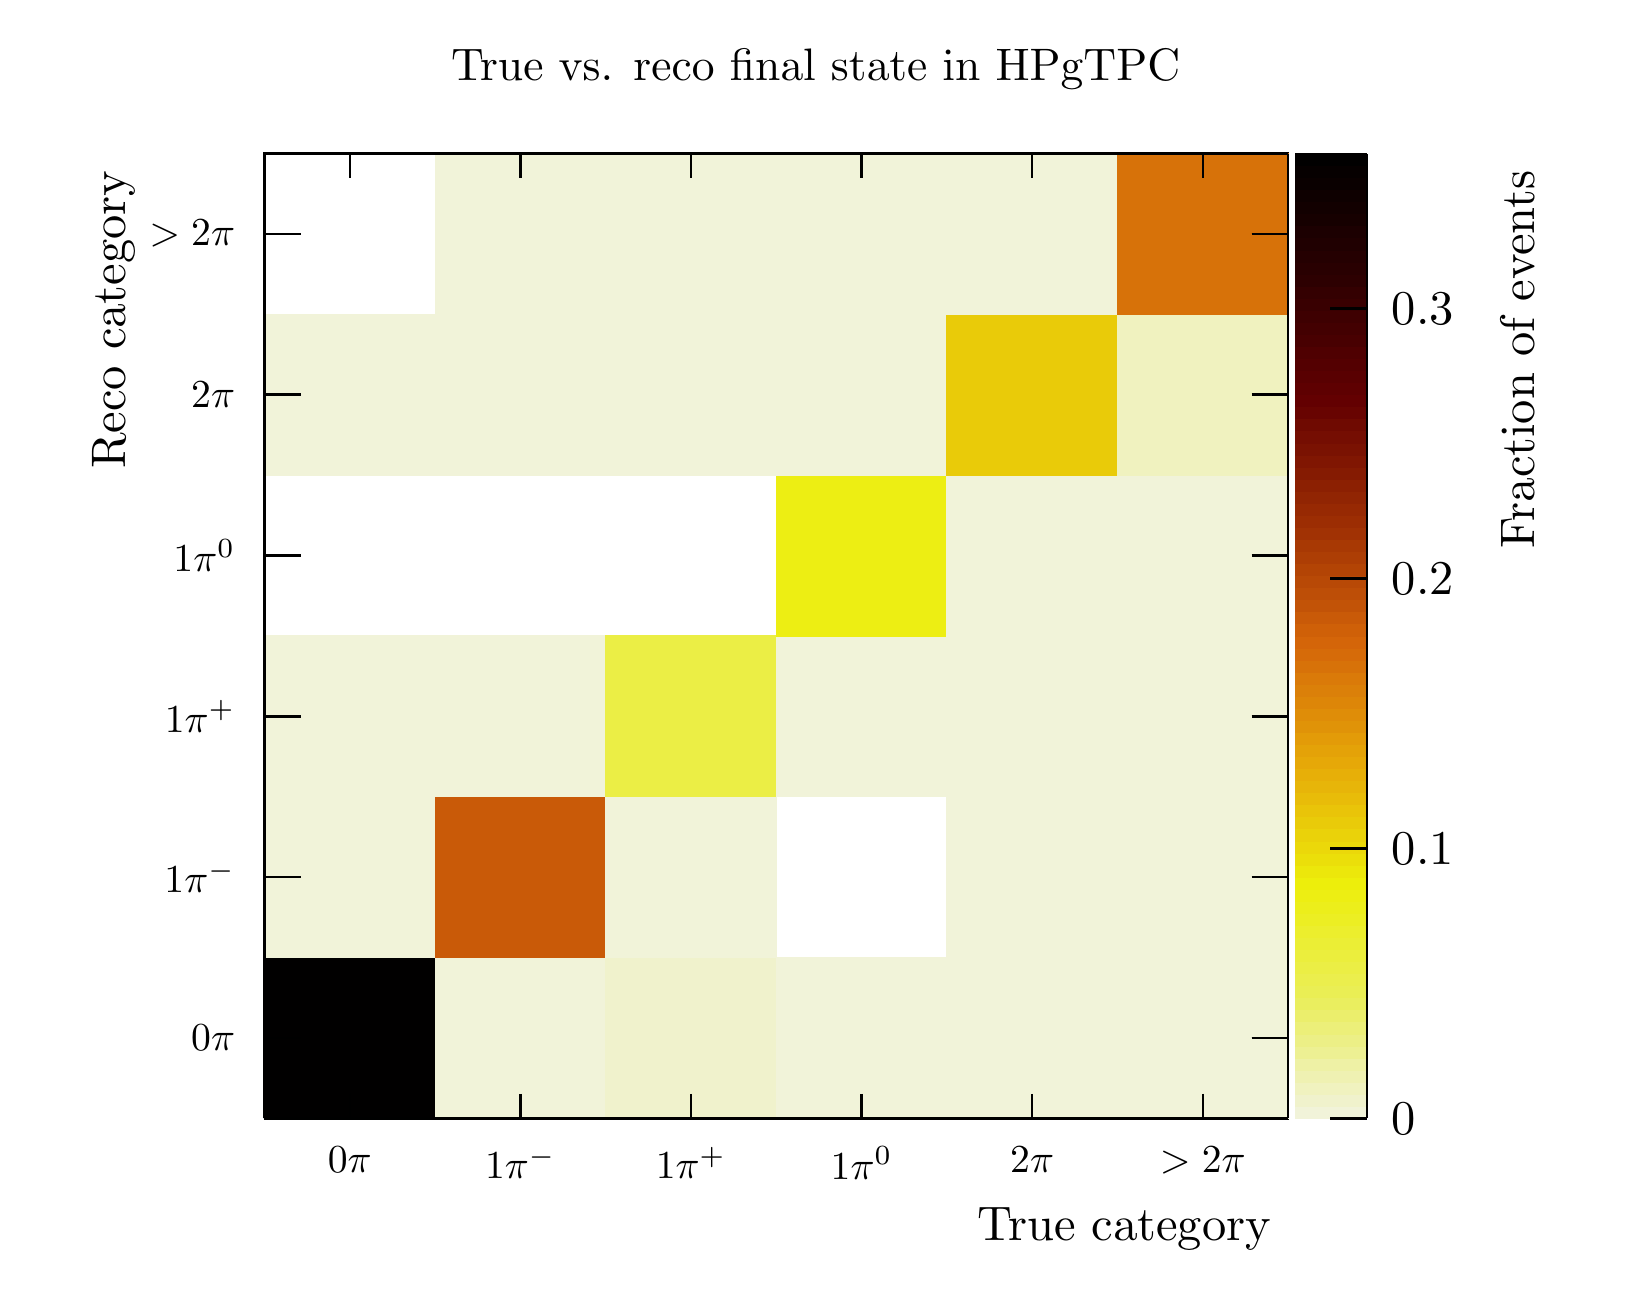
\begin{tikzpicture}
\pgfdeclareplotmark{cross} {
\pgfpathmoveto{\pgfpoint{-0.3\pgfplotmarksize}{\pgfplotmarksize}}
\pgfpathlineto{\pgfpoint{+0.3\pgfplotmarksize}{\pgfplotmarksize}}
\pgfpathlineto{\pgfpoint{+0.3\pgfplotmarksize}{0.3\pgfplotmarksize}}
\pgfpathlineto{\pgfpoint{+1\pgfplotmarksize}{0.3\pgfplotmarksize}}
\pgfpathlineto{\pgfpoint{+1\pgfplotmarksize}{-0.3\pgfplotmarksize}}
\pgfpathlineto{\pgfpoint{+0.3\pgfplotmarksize}{-0.3\pgfplotmarksize}}
\pgfpathlineto{\pgfpoint{+0.3\pgfplotmarksize}{-1.\pgfplotmarksize}}
\pgfpathlineto{\pgfpoint{-0.3\pgfplotmarksize}{-1.\pgfplotmarksize}}
\pgfpathlineto{\pgfpoint{-0.3\pgfplotmarksize}{-0.3\pgfplotmarksize}}
\pgfpathlineto{\pgfpoint{-1.\pgfplotmarksize}{-0.3\pgfplotmarksize}}
\pgfpathlineto{\pgfpoint{-1.\pgfplotmarksize}{0.3\pgfplotmarksize}}
\pgfpathlineto{\pgfpoint{-0.3\pgfplotmarksize}{0.3\pgfplotmarksize}}
\pgfpathclose
\pgfusepathqstroke
}
\pgfdeclareplotmark{cross*} {
\pgfpathmoveto{\pgfpoint{-0.3\pgfplotmarksize}{\pgfplotmarksize}}
\pgfpathlineto{\pgfpoint{+0.3\pgfplotmarksize}{\pgfplotmarksize}}
\pgfpathlineto{\pgfpoint{+0.3\pgfplotmarksize}{0.3\pgfplotmarksize}}
\pgfpathlineto{\pgfpoint{+1\pgfplotmarksize}{0.3\pgfplotmarksize}}
\pgfpathlineto{\pgfpoint{+1\pgfplotmarksize}{-0.3\pgfplotmarksize}}
\pgfpathlineto{\pgfpoint{+0.3\pgfplotmarksize}{-0.3\pgfplotmarksize}}
\pgfpathlineto{\pgfpoint{+0.3\pgfplotmarksize}{-1.\pgfplotmarksize}}
\pgfpathlineto{\pgfpoint{-0.3\pgfplotmarksize}{-1.\pgfplotmarksize}}
\pgfpathlineto{\pgfpoint{-0.3\pgfplotmarksize}{-0.3\pgfplotmarksize}}
\pgfpathlineto{\pgfpoint{-1.\pgfplotmarksize}{-0.3\pgfplotmarksize}}
\pgfpathlineto{\pgfpoint{-1.\pgfplotmarksize}{0.3\pgfplotmarksize}}
\pgfpathlineto{\pgfpoint{-0.3\pgfplotmarksize}{0.3\pgfplotmarksize}}
\pgfpathclose
\pgfusepathqfillstroke
}
\pgfdeclareplotmark{newstar} {
\pgfpathmoveto{\pgfqpoint{0pt}{\pgfplotmarksize}}
\pgfpathlineto{\pgfqpointpolar{44}{0.5\pgfplotmarksize}}
\pgfpathlineto{\pgfqpointpolar{18}{\pgfplotmarksize}}
\pgfpathlineto{\pgfqpointpolar{-20}{0.5\pgfplotmarksize}}
\pgfpathlineto{\pgfqpointpolar{-54}{\pgfplotmarksize}}
\pgfpathlineto{\pgfqpointpolar{-90}{0.5\pgfplotmarksize}}
\pgfpathlineto{\pgfqpointpolar{234}{\pgfplotmarksize}}
\pgfpathlineto{\pgfqpointpolar{198}{0.5\pgfplotmarksize}}
\pgfpathlineto{\pgfqpointpolar{162}{\pgfplotmarksize}}
\pgfpathlineto{\pgfqpointpolar{134}{0.5\pgfplotmarksize}}
\pgfpathclose
\pgfusepathqstroke
}
\pgfdeclareplotmark{newstar*} {
\pgfpathmoveto{\pgfqpoint{0pt}{\pgfplotmarksize}}
\pgfpathlineto{\pgfqpointpolar{44}{0.5\pgfplotmarksize}}
\pgfpathlineto{\pgfqpointpolar{18}{\pgfplotmarksize}}
\pgfpathlineto{\pgfqpointpolar{-20}{0.5\pgfplotmarksize}}
\pgfpathlineto{\pgfqpointpolar{-54}{\pgfplotmarksize}}
\pgfpathlineto{\pgfqpointpolar{-90}{0.5\pgfplotmarksize}}
\pgfpathlineto{\pgfqpointpolar{234}{\pgfplotmarksize}}
\pgfpathlineto{\pgfqpointpolar{198}{0.5\pgfplotmarksize}}
\pgfpathlineto{\pgfqpointpolar{162}{\pgfplotmarksize}}
\pgfpathlineto{\pgfqpointpolar{134}{0.5\pgfplotmarksize}}
\pgfpathclose
\pgfusepathqfillstroke
}
\definecolor{c}{rgb}{1,1,1};
\draw [color=c, fill=c] (0,0) rectangle (20,15.914);
\draw [color=c, fill=c] (3,2.06882) rectangle (16,14.3226);
\definecolor{c}{rgb}{0,0,0};
\draw [c,line width=0.9] (3,2.06882) -- (3,14.3226) -- (16,14.3226) -- (16,2.06882) -- (3,2.06882);
\definecolor{c}{rgb}{1,1,1};
\draw [color=c, fill=c] (3,2.06882) rectangle (16,14.3226);
\definecolor{c}{rgb}{0,0,0};
\draw [c,line width=0.9] (3,2.06882) -- (3,14.3226) -- (16,14.3226) -- (16,2.06882) -- (3,2.06882);
\definecolor{c}{rgb}{0.00551471,0,0.000122549};
\draw [color=c, fill=c] (3,2.06882) rectangle (5.16667,4.11111);
\definecolor{c}{rgb}{0.945984,0.951044,0.850727};
\draw [color=c, fill=c] (5.16667,2.06882) rectangle (7.33333,4.11111);
\definecolor{c}{rgb}{0.942948,0.949146,0.799494};
\draw [color=c, fill=c] (7.33333,2.06882) rectangle (9.5,4.11111);
\definecolor{c}{rgb}{0.945984,0.951044,0.850727};
\draw [color=c, fill=c] (9.5,2.06882) rectangle (11.6667,4.11111);
\draw [color=c, fill=c] (11.6667,2.06882) rectangle (13.8333,4.11111);
\draw [color=c, fill=c] (13.8333,2.06882) rectangle (16,4.11111);
\draw [color=c, fill=c] (3,4.11111) rectangle (5.16667,6.15341);
\definecolor{c}{rgb}{0.790196,0.354902,0.0308824};
\draw [color=c, fill=c] (5.16667,4.11111) rectangle (7.33333,6.15341);
\definecolor{c}{rgb}{0.945984,0.951044,0.850727};
\draw [color=c, fill=c] (7.33333,4.11111) rectangle (9.5,6.15341);
\draw [color=c, fill=c] (11.6667,4.11111) rectangle (13.8333,6.15341);
\draw [color=c, fill=c] (13.8333,4.11111) rectangle (16,6.15341);
\draw [color=c, fill=c] (3,6.15341) rectangle (5.16667,8.1957);
\draw [color=c, fill=c] (5.16667,6.15341) rectangle (7.33333,8.1957);
\definecolor{c}{rgb}{0.921324,0.933333,0.269608};
\draw [color=c, fill=c] (7.33333,6.15341) rectangle (9.5,8.1957);
\definecolor{c}{rgb}{0.945984,0.951044,0.850727};
\draw [color=c, fill=c] (9.5,6.15341) rectangle (11.6667,8.1957);
\draw [color=c, fill=c] (11.6667,6.15341) rectangle (13.8333,8.1957);
\draw [color=c, fill=c] (13.8333,6.15341) rectangle (16,8.1957);
\definecolor{c}{rgb}{0.928309,0.933333,0.0740196};
\draw [color=c, fill=c] (9.5,8.1957) rectangle (11.6667,10.238);
\definecolor{c}{rgb}{0.945984,0.951044,0.850727};
\draw [color=c, fill=c] (11.6667,8.1957) rectangle (13.8333,10.238);
\draw [color=c, fill=c] (13.8333,8.1957) rectangle (16,10.238);
\draw [color=c, fill=c] (3,10.238) rectangle (5.16667,12.2803);
\draw [color=c, fill=c] (5.16667,10.238) rectangle (7.33333,12.2803);
\draw [color=c, fill=c] (7.33333,10.238) rectangle (9.5,12.2803);
\draw [color=c, fill=c] (9.5,10.238) rectangle (11.6667,12.2803);
\definecolor{c}{rgb}{0.915686,0.796078,0.0372549};
\draw [color=c, fill=c] (11.6667,10.238) rectangle (13.8333,12.2803);
\definecolor{c}{rgb}{0.939911,0.947249,0.748261};
\draw [color=c, fill=c] (13.8333,10.238) rectangle (16,12.2803);
\definecolor{c}{rgb}{0.945984,0.951044,0.850727};
\draw [color=c, fill=c] (5.16667,12.2803) rectangle (7.33333,14.3226);
\draw [color=c, fill=c] (7.33333,12.2803) rectangle (9.5,14.3226);
\draw [color=c, fill=c] (9.5,12.2803) rectangle (11.6667,14.3226);
\draw [color=c, fill=c] (11.6667,12.2803) rectangle (13.8333,14.3226);
\definecolor{c}{rgb}{0.844608,0.445343,0.0345588};
\draw [color=c, fill=c] (13.8333,12.2803) rectangle (16,14.3226);
\definecolor{c}{rgb}{0,0,0};
\draw [c,line width=0.9] (3,2.06882) -- (16,2.06882);
\draw [anchor=north] (4.08333,1.88501) node[scale=1.43288, color=c, rotate=0]{$0\pi$};
\draw [anchor=north] (6.25,1.88501) node[scale=1.43288, color=c, rotate=0]{$1\pi^{-}$};
\draw [anchor=north] (8.41667,1.88501) node[scale=1.43288, color=c, rotate=0]{$1\pi^{+}$};
\draw [anchor=north] (10.5833,1.88501) node[scale=1.43288, color=c, rotate=0]{$1\pi^{0}$};
\draw [anchor=north] (12.75,1.88501) node[scale=1.43288, color=c, rotate=0]{$2\pi$};
\draw [anchor=north] (14.9167,1.88501) node[scale=1.43288, color=c, rotate=0]{$>2\pi$};
\draw [c,line width=0.9] (4.08333,2.37914) -- (4.08333,2.06882);
\draw [c,line width=0.9] (6.25,2.37914) -- (6.25,2.06882);
\draw [c,line width=0.9] (8.41667,2.37914) -- (8.41667,2.06882);
\draw [c,line width=0.9] (10.5833,2.37914) -- (10.5833,2.06882);
\draw [c,line width=0.9] (12.75,2.37914) -- (12.75,2.06882);
\draw [c,line width=0.9] (14.9167,2.37914) -- (14.9167,2.06882);
\draw [c,line width=0.9] (4.08333,2.37914) -- (4.08333,2.06882);
\draw [c,line width=0.9] (14.9167,2.37914) -- (14.9167,2.06882);
\draw [anchor= east] (16,0.668387) node[scale=1.7513, color=c, rotate=0]{ True category};
\draw [c,line width=0.9] (3,14.3226) -- (16,14.3226);
\draw [c,line width=0.9] (4.08333,14.0123) -- (4.08333,14.3226);
\draw [c,line width=0.9] (6.25,14.0123) -- (6.25,14.3226);
\draw [c,line width=0.9] (8.41667,14.0123) -- (8.41667,14.3226);
\draw [c,line width=0.9] (10.5833,14.0123) -- (10.5833,14.3226);
\draw [c,line width=0.9] (12.75,14.0123) -- (12.75,14.3226);
\draw [c,line width=0.9] (14.9167,14.0123) -- (14.9167,14.3226);
\draw [c,line width=0.9] (4.08333,14.0123) -- (4.08333,14.3226);
\draw [c,line width=0.9] (14.9167,14.0123) -- (14.9167,14.3226);
\draw [c,line width=0.9] (3,2.06882) -- (3,14.3226);
\draw [anchor= east] (2.805,3.08996) node[scale=1.43288, color=c, rotate=0]{$0\pi$};
\draw [anchor= east] (2.805,5.13226) node[scale=1.43288, color=c, rotate=0]{$1\pi^{-}$};
\draw [anchor= east] (2.805,7.17455) node[scale=1.43288, color=c, rotate=0]{$1\pi^{+}$};
\draw [anchor= east] (2.805,9.21685) node[scale=1.43288, color=c, rotate=0]{$1\pi^{0}$};
\draw [anchor= east] (2.805,11.2591) node[scale=1.43288, color=c, rotate=0]{$2\pi$};
\draw [anchor= east] (2.805,13.3014) node[scale=1.43288, color=c, rotate=0]{$>2\pi$};
\draw [c,line width=0.9] (3.462,3.08996) -- (3,3.08996);
\draw [c,line width=0.9] (3.462,5.13226) -- (3,5.13226);
\draw [c,line width=0.9] (3.462,7.17455) -- (3,7.17455);
\draw [c,line width=0.9] (3.462,9.21685) -- (3,9.21685);
\draw [c,line width=0.9] (3.462,11.2591) -- (3,11.2591);
\draw [c,line width=0.9] (3.462,13.3014) -- (3,13.3014);
\draw [c,line width=0.9] (3.462,3.08996) -- (3,3.08996);
\draw [c,line width=0.9] (3.462,13.3014) -- (3,13.3014);
\draw [anchor= east] (1.08,14.3226) node[scale=1.7513, color=c, rotate=90]{ Reco category};
\draw [c,line width=0.9] (16,2.06882) -- (16,14.3226);
\draw [c,line width=0.9] (15.538,3.08996) -- (16,3.08996);
\draw [c,line width=0.9] (15.538,5.13226) -- (16,5.13226);
\draw [c,line width=0.9] (15.538,7.17455) -- (16,7.17455);
\draw [c,line width=0.9] (15.538,9.21685) -- (16,9.21685);
\draw [c,line width=0.9] (15.538,11.2591) -- (16,11.2591);
\draw [c,line width=0.9] (15.538,13.3014) -- (16,13.3014);
\draw [c,line width=0.9] (15.538,3.08996) -- (16,3.08996);
\draw [c,line width=0.9] (15.538,13.3014) -- (16,13.3014);
\definecolor{c}{rgb}{0.945984,0.951044,0.850727};
\draw [color=c, fill=c] (16.1,2.06882) rectangle (17,2.22199);
\definecolor{c}{rgb}{0.942948,0.949146,0.799494};
\draw [color=c, fill=c] (16.1,2.22199) rectangle (17,2.37516);
\definecolor{c}{rgb}{0.939911,0.947249,0.748261};
\draw [color=c, fill=c] (16.1,2.37516) rectangle (17,2.52833);
\definecolor{c}{rgb}{0.936875,0.945351,0.697027};
\draw [color=c, fill=c] (16.1,2.52833) rectangle (17,2.68151);
\definecolor{c}{rgb}{0.933839,0.943453,0.645794};
\draw [color=c, fill=c] (16.1,2.68151) rectangle (17,2.83468);
\definecolor{c}{rgb}{0.929791,0.940923,0.577483};
\draw [color=c, fill=c] (16.1,2.83468) rectangle (17,2.98785);
\definecolor{c}{rgb}{0.926755,0.939026,0.526249};
\draw [color=c, fill=c] (16.1,2.98785) rectangle (17,3.14102);
\definecolor{c}{rgb}{0.923719,0.937128,0.475016};
\draw [color=c, fill=c] (16.1,3.14102) rectangle (17,3.29419);
\definecolor{c}{rgb}{0.920683,0.935231,0.423782};
\draw [color=c, fill=c] (16.1,3.29419) rectangle (17,3.44737);
\definecolor{c}{rgb}{0.917647,0.933333,0.372549};
\draw [color=c, fill=c] (16.1,3.44737) rectangle (17,3.60054);
\definecolor{c}{rgb}{0.919118,0.933333,0.331373};
\draw [color=c, fill=c] (16.1,3.60054) rectangle (17,3.75371);
\definecolor{c}{rgb}{0.920221,0.933333,0.30049};
\draw [color=c, fill=c] (16.1,3.75371) rectangle (17,3.90688);
\definecolor{c}{rgb}{0.921324,0.933333,0.269608};
\draw [color=c, fill=c] (16.1,3.90688) rectangle (17,4.06005);
\definecolor{c}{rgb}{0.922426,0.933333,0.238725};
\draw [color=c, fill=c] (16.1,4.06005) rectangle (17,4.21323);
\definecolor{c}{rgb}{0.923529,0.933333,0.207843};
\draw [color=c, fill=c] (16.1,4.21323) rectangle (17,4.3664);
\definecolor{c}{rgb}{0.924632,0.933333,0.176961};
\draw [color=c, fill=c] (16.1,4.3664) rectangle (17,4.51957);
\definecolor{c}{rgb}{0.926103,0.933333,0.135784};
\draw [color=c, fill=c] (16.1,4.51957) rectangle (17,4.67274);
\definecolor{c}{rgb}{0.927206,0.933333,0.104902};
\draw [color=c, fill=c] (16.1,4.67274) rectangle (17,4.82591);
\definecolor{c}{rgb}{0.928309,0.933333,0.0740196};
\draw [color=c, fill=c] (16.1,4.82591) rectangle (17,4.97909);
\definecolor{c}{rgb}{0.929412,0.933333,0.0431373};
\draw [color=c, fill=c] (16.1,4.97909) rectangle (17,5.13226);
\definecolor{c}{rgb}{0.926838,0.907598,0.0420343};
\draw [color=c, fill=c] (16.1,5.13226) rectangle (17,5.28543);
\definecolor{c}{rgb}{0.923407,0.873284,0.0405637};
\draw [color=c, fill=c] (16.1,5.28543) rectangle (17,5.4386);
\definecolor{c}{rgb}{0.920833,0.847549,0.0394608};
\draw [color=c, fill=c] (16.1,5.4386) rectangle (17,5.59177);
\definecolor{c}{rgb}{0.91826,0.821814,0.0383578};
\draw [color=c, fill=c] (16.1,5.59177) rectangle (17,5.74495);
\definecolor{c}{rgb}{0.915686,0.796078,0.0372549};
\draw [color=c, fill=c] (16.1,5.74495) rectangle (17,5.89812);
\definecolor{c}{rgb}{0.913113,0.770343,0.036152};
\draw [color=c, fill=c] (16.1,5.89812) rectangle (17,6.05129);
\definecolor{c}{rgb}{0.909681,0.736029,0.0346814};
\draw [color=c, fill=c] (16.1,6.05129) rectangle (17,6.20446);
\definecolor{c}{rgb}{0.907108,0.710294,0.0335784};
\draw [color=c, fill=c] (16.1,6.20446) rectangle (17,6.35763);
\definecolor{c}{rgb}{0.904534,0.684559,0.0324755};
\draw [color=c, fill=c] (16.1,6.35763) rectangle (17,6.51081);
\definecolor{c}{rgb}{0.901961,0.658824,0.0313726};
\draw [color=c, fill=c] (16.1,6.51081) rectangle (17,6.66398);
\definecolor{c}{rgb}{0.895343,0.634191,0.0317402};
\draw [color=c, fill=c] (16.1,6.66398) rectangle (17,6.81715);
\definecolor{c}{rgb}{0.888726,0.609559,0.0321078};
\draw [color=c, fill=c] (16.1,6.81715) rectangle (17,6.97032);
\definecolor{c}{rgb}{0.879902,0.576716,0.032598};
\draw [color=c, fill=c] (16.1,6.97032) rectangle (17,7.12349);
\definecolor{c}{rgb}{0.873284,0.552083,0.0329657};
\draw [color=c, fill=c] (16.1,7.12349) rectangle (17,7.27667);
\definecolor{c}{rgb}{0.866667,0.527451,0.0333333};
\draw [color=c, fill=c] (16.1,7.27667) rectangle (17,7.42984);
\definecolor{c}{rgb}{0.860049,0.502819,0.033701};
\draw [color=c, fill=c] (16.1,7.42984) rectangle (17,7.58301);
\definecolor{c}{rgb}{0.853431,0.478186,0.0340686};
\draw [color=c, fill=c] (16.1,7.58301) rectangle (17,7.73618);
\definecolor{c}{rgb}{0.844608,0.445343,0.0345588};
\draw [color=c, fill=c] (16.1,7.73618) rectangle (17,7.88935);
\definecolor{c}{rgb}{0.83799,0.420711,0.0349265};
\draw [color=c, fill=c] (16.1,7.88935) rectangle (17,8.04253);
\definecolor{c}{rgb}{0.831373,0.396078,0.0352941};
\draw [color=c, fill=c] (16.1,8.04253) rectangle (17,8.1957);
\definecolor{c}{rgb}{0.810784,0.37549,0.0330882};
\draw [color=c, fill=c] (16.1,8.1957) rectangle (17,8.34887);
\definecolor{c}{rgb}{0.790196,0.354902,0.0308824};
\draw [color=c, fill=c] (16.1,8.34887) rectangle (17,8.50204);
\definecolor{c}{rgb}{0.762745,0.327451,0.0279412};
\draw [color=c, fill=c] (16.1,8.50204) rectangle (17,8.65522);
\definecolor{c}{rgb}{0.742157,0.306863,0.0257353};
\draw [color=c, fill=c] (16.1,8.65522) rectangle (17,8.80839);
\definecolor{c}{rgb}{0.721569,0.286275,0.0235294};
\draw [color=c, fill=c] (16.1,8.80839) rectangle (17,8.96156);
\definecolor{c}{rgb}{0.70098,0.265686,0.0213235};
\draw [color=c, fill=c] (16.1,8.96156) rectangle (17,9.11473);
\definecolor{c}{rgb}{0.680392,0.245098,0.0191176};
\draw [color=c, fill=c] (16.1,9.11473) rectangle (17,9.2679);
\definecolor{c}{rgb}{0.659804,0.22451,0.0169118};
\draw [color=c, fill=c] (16.1,9.2679) rectangle (17,9.42107);
\definecolor{c}{rgb}{0.632353,0.197059,0.0139706};
\draw [color=c, fill=c] (16.1,9.42107) rectangle (17,9.57425);
\definecolor{c}{rgb}{0.611765,0.176471,0.0117647};
\draw [color=c, fill=c] (16.1,9.57425) rectangle (17,9.72742);
\definecolor{c}{rgb}{0.590809,0.159926,0.0110294};
\draw [color=c, fill=c] (16.1,9.72742) rectangle (17,9.88059);
\definecolor{c}{rgb}{0.569853,0.143382,0.0102941};
\draw [color=c, fill=c] (16.1,9.88059) rectangle (17,10.0338);
\definecolor{c}{rgb}{0.548897,0.126838,0.00955882};
\draw [color=c, fill=c] (16.1,10.0338) rectangle (17,10.1869);
\definecolor{c}{rgb}{0.520956,0.104779,0.00857843};
\draw [color=c, fill=c] (16.1,10.1869) rectangle (17,10.3401);
\definecolor{c}{rgb}{0.5,0.0882353,0.00784314};
\draw [color=c, fill=c] (16.1,10.3401) rectangle (17,10.4933);
\definecolor{c}{rgb}{0.479044,0.0716912,0.00710784};
\draw [color=c, fill=c] (16.1,10.4933) rectangle (17,10.6465);
\definecolor{c}{rgb}{0.458088,0.0551471,0.00637255};
\draw [color=c, fill=c] (16.1,10.6465) rectangle (17,10.7996);
\definecolor{c}{rgb}{0.437132,0.0386029,0.00563726};
\draw [color=c, fill=c] (16.1,10.7996) rectangle (17,10.9528);
\definecolor{c}{rgb}{0.409191,0.0165441,0.00465686};
\draw [color=c, fill=c] (16.1,10.9528) rectangle (17,11.106);
\definecolor{c}{rgb}{0.388235,0,0.00392157};
\draw [color=c, fill=c] (16.1,11.106) rectangle (17,11.2591);
\definecolor{c}{rgb}{0.368382,0,0.00392157};
\draw [color=c, fill=c] (16.1,11.2591) rectangle (17,11.4123);
\definecolor{c}{rgb}{0.348529,0,0.00392157};
\draw [color=c, fill=c] (16.1,11.4123) rectangle (17,11.5655);
\definecolor{c}{rgb}{0.328676,0,0.00392157};
\draw [color=c, fill=c] (16.1,11.5655) rectangle (17,11.7187);
\definecolor{c}{rgb}{0.308824,0,0.00392157};
\draw [color=c, fill=c] (16.1,11.7187) rectangle (17,11.8718);
\definecolor{c}{rgb}{0.282353,0,0.00392157};
\draw [color=c, fill=c] (16.1,11.8718) rectangle (17,12.025);
\definecolor{c}{rgb}{0.2625,0,0.00392157};
\draw [color=c, fill=c] (16.1,12.025) rectangle (17,12.1782);
\definecolor{c}{rgb}{0.242647,0,0.00392157};
\draw [color=c, fill=c] (16.1,12.1782) rectangle (17,12.3313);
\definecolor{c}{rgb}{0.222794,0,0.00392157};
\draw [color=c, fill=c] (16.1,12.3313) rectangle (17,12.4845);
\definecolor{c}{rgb}{0.202941,0,0.00392157};
\draw [color=c, fill=c] (16.1,12.4845) rectangle (17,12.6377);
\definecolor{c}{rgb}{0.176471,0,0.00392157};
\draw [color=c, fill=c] (16.1,12.6377) rectangle (17,12.7909);
\definecolor{c}{rgb}{0.159926,0,0.00355392};
\draw [color=c, fill=c] (16.1,12.7909) rectangle (17,12.944);
\definecolor{c}{rgb}{0.143382,0,0.00318627};
\draw [color=c, fill=c] (16.1,12.944) rectangle (17,13.0972);
\definecolor{c}{rgb}{0.126838,0,0.00281863};
\draw [color=c, fill=c] (16.1,13.0972) rectangle (17,13.2504);
\definecolor{c}{rgb}{0.110294,0,0.00245098};
\draw [color=c, fill=c] (16.1,13.2504) rectangle (17,13.4035);
\definecolor{c}{rgb}{0.0882353,0,0.00196078};
\draw [color=c, fill=c] (16.1,13.4035) rectangle (17,13.5567);
\definecolor{c}{rgb}{0.0716912,0,0.00159314};
\draw [color=c, fill=c] (16.1,13.5567) rectangle (17,13.7099);
\definecolor{c}{rgb}{0.0551471,0,0.00122549};
\draw [color=c, fill=c] (16.1,13.7099) rectangle (17,13.8631);
\definecolor{c}{rgb}{0.0386029,0,0.000857843};
\draw [color=c, fill=c] (16.1,13.8631) rectangle (17,14.0162);
\definecolor{c}{rgb}{0.0220588,0,0.000490196};
\draw [color=c, fill=c] (16.1,14.0162) rectangle (17,14.1694);
\definecolor{c}{rgb}{0.00551471,0,0.000122549};
\draw [color=c, fill=c] (16.1,14.1694) rectangle (17,14.3226);
\definecolor{c}{rgb}{0,0,0};
\draw [c,line width=0.9] (17,2.06882) -- (17,14.3226);
\draw [c,line width=0.9] (16.538,2.06882) -- (17,2.06882);
\draw [c,line width=0.9] (16.538,5.49645) -- (17,5.49645);
\draw [c,line width=0.9] (16.538,8.92408) -- (17,8.92408);
\draw [c,line width=0.9] (16.538,12.3517) -- (17,12.3517);
\draw [c,line width=0.9] (16.538,12.3517) -- (17,12.3517);
\draw [anchor= west] (17.1,2.06882) node[scale=1.7513, color=c, rotate=0]{0};
\draw [anchor= west] (17.1,5.49645) node[scale=1.7513, color=c, rotate=0]{0.1};
\draw [anchor= west] (17.1,8.92408) node[scale=1.7513, color=c, rotate=0]{0.2};
\draw [anchor= west] (17.1,12.3517) node[scale=1.7513, color=c, rotate=0]{0.3};
\draw [anchor= east] (18.92,14.3226) node[scale=1.7513, color=c, rotate=90]{ Fraction of events};
\definecolor{c}{rgb}{1,1,1};
\draw [color=c, fill=c] (2,14.9591) rectangle (18,15.8344);
\definecolor{c}{rgb}{0,0,0};
\draw (10,15.3968) node[scale=1.64516, color=c, rotate=0]{True vs. reco final state in HPgTPC};
\end{tikzpicture}

%		\end{adjustbox}
%	\end{minipage}
%	\caption[True and reconstructed event categories for ND-GAr events]{Left: True and reconstructed final state pion multiplicities in ND-GAr with the neutrino beam in FHC mode. Right: True and reconstructed final state pion multiplicities in ND-GAr with the neutrino beam in RHC mode.}
%	\label{fig:eventCats}
%\end{figure}

The reconstructed squared momentum transfer for CC muon neutrino events is defined as
\begin{equation}
Q^{2}_{\textrm{reco}} = 2E_{\nu, \textrm{reco}} \left( E_{\mu, \textrm{reco}} - p_{\mu, \textrm{reco}} \cos \left( \theta_{\mu, \textrm{reco}} \right) \right) - m_{\mu}^{2}
\end{equation}
where $E_{\nu, \textrm{reco}}$ is the sum of the reconstructed muon energy and the reconstructed final state hadron energies, $E_{\mu, \textrm{reco}}$ and $p_{\mu, \textrm{reco}}$ are the reconstructed energy and momentum of the final state muon and $\theta_{\mu, \textrm{reco}}$ is the reconstructed angle between the muon and the neutrino beam.

The mock data generator detailed in \citesec{sec:dune_ndrwt:bdt} used to reweight events to give an approximation of NuWro data.
A distribution of $Q^{2}_{\textrm{reco}}$ is then constructed for each of the nominal GENIE sample and the reweighted sample. 
The ratio between the two samples is then taken and plotted. 

These ratios are shown in \citefigL{fig:Q2CompFhc} and \citefigL{fig:Q2CompRhc}. 
Here, one can clearly see that, for all final states apart from $0\pi$, clear differences between GENIE and NuWro are observable.

The errors on the points resulting from confusion between the final states are estimated using the following method.
Distributions of $Q^{2}_{\textrm{reco}}$ are produced for each of the $i$ true final states for GENIE and NuWro and then the ratio between the two is calculated as before.
For the final state in question, $x$, the value of $n$th bin in this histogram is taken as the true central value $R_{\textrm{CV}, x}(n)$.
The variance of the $n$th bin is calculated as follows:
\begin{equation}
	\sigma_{x}^{2}(n) = \sum_{i=1}^{5} \left( R_{a}(n) - R_{\textrm{CV}, x}(n) \right)^{2} * \frac{M_{i x}}{N_{x}}
\end{equation}
where $i$ runs over the final states and $M$ is the smearing matrix in \citefig{fig:confusMatPi} corresponding to the correct horn current.
The constant $N$ is a normalisation factor determined by summing the bin contents of row $x$ of the smearing matrix. 

Additionally, \citefigR{fig:Q2CompFhc} and \citefigR{fig:Q2CompRhc} show the equivalent distributions for true selections and variables. 
One can see that these distributions replicate many of the features of the reconstructed distributions well.

\begin{figure}[h]
	\begin{minipage}[t]{.5\linewidth}
		\begin{adjustbox}{max totalsize=\linewidth, center}
			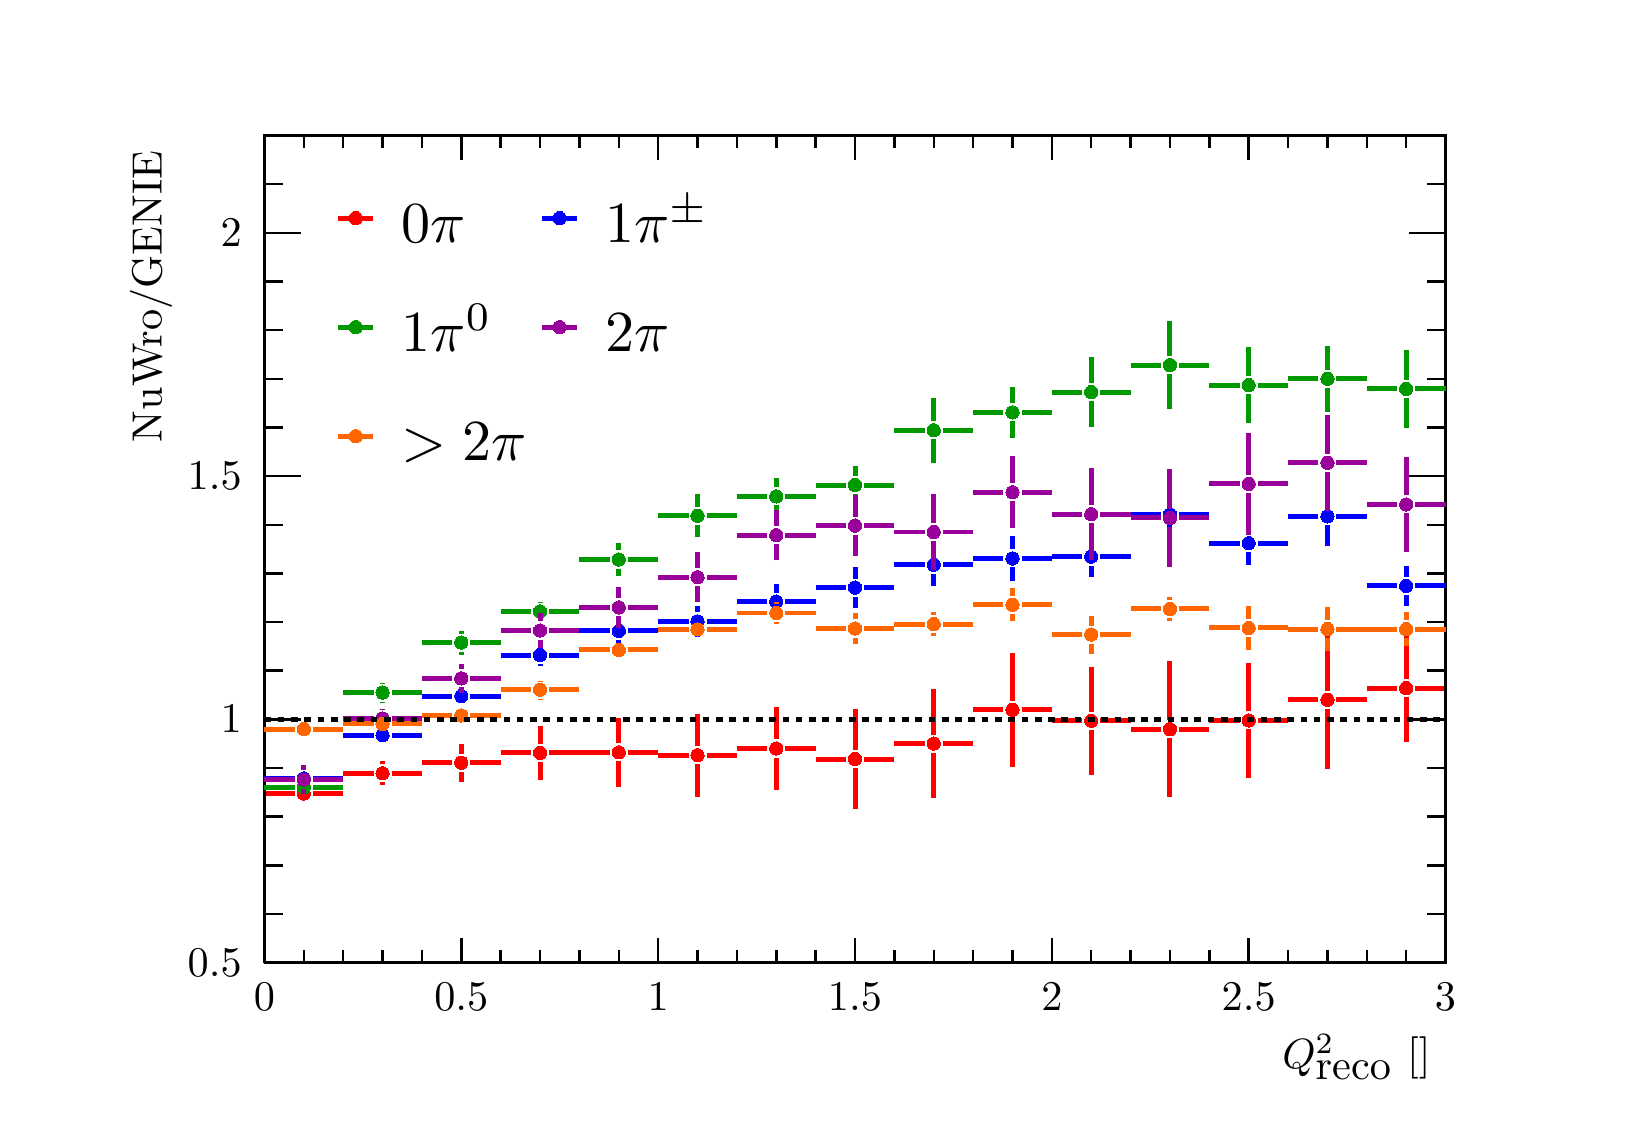
\begin{tikzpicture}
\pgfdeclareplotmark{cross} {
\pgfpathmoveto{\pgfpoint{-0.3\pgfplotmarksize}{\pgfplotmarksize}}
\pgfpathlineto{\pgfpoint{+0.3\pgfplotmarksize}{\pgfplotmarksize}}
\pgfpathlineto{\pgfpoint{+0.3\pgfplotmarksize}{0.3\pgfplotmarksize}}
\pgfpathlineto{\pgfpoint{+1\pgfplotmarksize}{0.3\pgfplotmarksize}}
\pgfpathlineto{\pgfpoint{+1\pgfplotmarksize}{-0.3\pgfplotmarksize}}
\pgfpathlineto{\pgfpoint{+0.3\pgfplotmarksize}{-0.3\pgfplotmarksize}}
\pgfpathlineto{\pgfpoint{+0.3\pgfplotmarksize}{-1.\pgfplotmarksize}}
\pgfpathlineto{\pgfpoint{-0.3\pgfplotmarksize}{-1.\pgfplotmarksize}}
\pgfpathlineto{\pgfpoint{-0.3\pgfplotmarksize}{-0.3\pgfplotmarksize}}
\pgfpathlineto{\pgfpoint{-1.\pgfplotmarksize}{-0.3\pgfplotmarksize}}
\pgfpathlineto{\pgfpoint{-1.\pgfplotmarksize}{0.3\pgfplotmarksize}}
\pgfpathlineto{\pgfpoint{-0.3\pgfplotmarksize}{0.3\pgfplotmarksize}}
\pgfpathclose
\pgfusepathqstroke
}
\pgfdeclareplotmark{cross*} {
\pgfpathmoveto{\pgfpoint{-0.3\pgfplotmarksize}{\pgfplotmarksize}}
\pgfpathlineto{\pgfpoint{+0.3\pgfplotmarksize}{\pgfplotmarksize}}
\pgfpathlineto{\pgfpoint{+0.3\pgfplotmarksize}{0.3\pgfplotmarksize}}
\pgfpathlineto{\pgfpoint{+1\pgfplotmarksize}{0.3\pgfplotmarksize}}
\pgfpathlineto{\pgfpoint{+1\pgfplotmarksize}{-0.3\pgfplotmarksize}}
\pgfpathlineto{\pgfpoint{+0.3\pgfplotmarksize}{-0.3\pgfplotmarksize}}
\pgfpathlineto{\pgfpoint{+0.3\pgfplotmarksize}{-1.\pgfplotmarksize}}
\pgfpathlineto{\pgfpoint{-0.3\pgfplotmarksize}{-1.\pgfplotmarksize}}
\pgfpathlineto{\pgfpoint{-0.3\pgfplotmarksize}{-0.3\pgfplotmarksize}}
\pgfpathlineto{\pgfpoint{-1.\pgfplotmarksize}{-0.3\pgfplotmarksize}}
\pgfpathlineto{\pgfpoint{-1.\pgfplotmarksize}{0.3\pgfplotmarksize}}
\pgfpathlineto{\pgfpoint{-0.3\pgfplotmarksize}{0.3\pgfplotmarksize}}
\pgfpathclose
\pgfusepathqfillstroke
}
\pgfdeclareplotmark{newstar} {
\pgfpathmoveto{\pgfqpoint{0pt}{\pgfplotmarksize}}
\pgfpathlineto{\pgfqpointpolar{44}{0.5\pgfplotmarksize}}
\pgfpathlineto{\pgfqpointpolar{18}{\pgfplotmarksize}}
\pgfpathlineto{\pgfqpointpolar{-20}{0.5\pgfplotmarksize}}
\pgfpathlineto{\pgfqpointpolar{-54}{\pgfplotmarksize}}
\pgfpathlineto{\pgfqpointpolar{-90}{0.5\pgfplotmarksize}}
\pgfpathlineto{\pgfqpointpolar{234}{\pgfplotmarksize}}
\pgfpathlineto{\pgfqpointpolar{198}{0.5\pgfplotmarksize}}
\pgfpathlineto{\pgfqpointpolar{162}{\pgfplotmarksize}}
\pgfpathlineto{\pgfqpointpolar{134}{0.5\pgfplotmarksize}}
\pgfpathclose
\pgfusepathqstroke
}
\pgfdeclareplotmark{newstar*} {
\pgfpathmoveto{\pgfqpoint{0pt}{\pgfplotmarksize}}
\pgfpathlineto{\pgfqpointpolar{44}{0.5\pgfplotmarksize}}
\pgfpathlineto{\pgfqpointpolar{18}{\pgfplotmarksize}}
\pgfpathlineto{\pgfqpointpolar{-20}{0.5\pgfplotmarksize}}
\pgfpathlineto{\pgfqpointpolar{-54}{\pgfplotmarksize}}
\pgfpathlineto{\pgfqpointpolar{-90}{0.5\pgfplotmarksize}}
\pgfpathlineto{\pgfqpointpolar{234}{\pgfplotmarksize}}
\pgfpathlineto{\pgfqpointpolar{198}{0.5\pgfplotmarksize}}
\pgfpathlineto{\pgfqpointpolar{162}{\pgfplotmarksize}}
\pgfpathlineto{\pgfqpointpolar{134}{0.5\pgfplotmarksize}}
\pgfpathclose
\pgfusepathqfillstroke
}
\definecolor{c}{rgb}{1,1,1};
\draw [color=c, fill=c] (0,0) rectangle (20,13.639);
\draw [color=c, fill=c] (3,1.77307) rectangle (18,12.2751);
\definecolor{c}{rgb}{0,0,0};
\draw [c,line width=0.9] (3,1.77307) -- (3,12.2751) -- (18,12.2751) -- (18,1.77307) -- (3,1.77307);
\definecolor{c}{rgb}{1,1,1};
\draw [color=c, fill=c] (3,1.77307) rectangle (18,12.2751);
\definecolor{c}{rgb}{0,0,0};
\draw [c,line width=0.9] (3,1.77307) -- (3,12.2751) -- (18,12.2751) -- (18,1.77307) -- (3,1.77307);
\definecolor{c}{rgb}{1,0,0};
\draw [c,line width=1.8] (3,3.91911) -- (3.38539,3.91911);
\draw [c,line width=1.8] (3.61461,3.91911) -- (4,3.91911);
\foreach \P in {(3.5,3.91911)}{\draw[mark options={color=c,fill=c},mark size=2.402402pt, line width=0.000000pt, mark=*] plot coordinates {\P};}
\draw [c,line width=1.8] (4.5,4.02491) -- (4.5,4.06197);
\draw [c,line width=1.8] (4.5,4.2912) -- (4.5,4.32827);
\draw [c,line width=1.8] (4,4.17659) -- (4.38539,4.17659);
\draw [c,line width=1.8] (4.61461,4.17659) -- (5,4.17659);
\foreach \P in {(4.5,4.17659)}{\draw[mark options={color=c,fill=c},mark size=2.402402pt, line width=0.000000pt, mark=*] plot coordinates {\P};}
\draw [c,line width=1.8] (5.5,4.06967) -- (5.5,4.19653);
\draw [c,line width=1.8] (5.5,4.42576) -- (5.5,4.55262);
\draw [c,line width=1.8] (5,4.31115) -- (5.38539,4.31115);
\draw [c,line width=1.8] (5.61461,4.31115) -- (6,4.31115);
\foreach \P in {(5.5,4.31115)}{\draw[mark options={color=c,fill=c},mark size=2.402402pt, line width=0.000000pt, mark=*] plot coordinates {\P};}
\draw [c,line width=1.8] (6.5,4.09054) -- (6.5,4.32215);
\draw [c,line width=1.8] (6.5,4.55138) -- (6.5,4.78299);
\draw [c,line width=1.8] (6,4.43676) -- (6.38539,4.43676);
\draw [c,line width=1.8] (6.61461,4.43676) -- (7,4.43676);
\foreach \P in {(6.5,4.43676)}{\draw[mark options={color=c,fill=c},mark size=2.402402pt, line width=0.000000pt, mark=*] plot coordinates {\P};}
\draw [c,line width=1.8] (7.5,4.00439) -- (7.5,4.32806);
\draw [c,line width=1.8] (7.5,4.55729) -- (7.5,4.88095);
\draw [c,line width=1.8] (7,4.44267) -- (7.38539,4.44267);
\draw [c,line width=1.8] (7.61461,4.44267) -- (8,4.44267);
\foreach \P in {(7.5,4.44267)}{\draw[mark options={color=c,fill=c},mark size=2.402402pt, line width=0.000000pt, mark=*] plot coordinates {\P};}
\draw [c,line width=1.8] (8.5,3.88168) -- (8.5,4.2921);
\draw [c,line width=1.8] (8.5,4.52133) -- (8.5,4.93175);
\draw [c,line width=1.8] (8,4.40671) -- (8.38539,4.40671);
\draw [c,line width=1.8] (8.61461,4.40671) -- (9,4.40671);
\foreach \P in {(8.5,4.40671)}{\draw[mark options={color=c,fill=c},mark size=2.402402pt, line width=0.000000pt, mark=*] plot coordinates {\P};}
\draw [c,line width=1.8] (9.5,3.95924) -- (9.5,4.37703);
\draw [c,line width=1.8] (9.5,4.60626) -- (9.5,5.02405);
\draw [c,line width=1.8] (9,4.49165) -- (9.38539,4.49165);
\draw [c,line width=1.8] (9.61461,4.49165) -- (10,4.49165);
\foreach \P in {(9.5,4.49165)}{\draw[mark options={color=c,fill=c},mark size=2.402402pt, line width=0.000000pt, mark=*] plot coordinates {\P};}
\draw [c,line width=1.8] (10.5,3.72077) -- (10.5,4.24284);
\draw [c,line width=1.8] (10.5,4.47207) -- (10.5,4.99414);
\draw [c,line width=1.8] (10,4.35746) -- (10.3854,4.35746);
\draw [c,line width=1.8] (10.6146,4.35746) -- (11,4.35746);
\foreach \P in {(10.5,4.35746)}{\draw[mark options={color=c,fill=c},mark size=2.402402pt, line width=0.000000pt, mark=*] plot coordinates {\P};}
\draw [c,line width=1.8] (11.5,3.86667) -- (11.5,4.43937);
\draw [c,line width=1.8] (11.5,4.6686) -- (11.5,5.24131);
\draw [c,line width=1.8] (11,4.55399) -- (11.3854,4.55399);
\draw [c,line width=1.8] (11.6146,4.55399) -- (12,4.55399);
\foreach \P in {(11.5,4.55399)}{\draw[mark options={color=c,fill=c},mark size=2.402402pt, line width=0.000000pt, mark=*] plot coordinates {\P};}
\draw [c,line width=1.8] (12.5,4.26285) -- (12.5,4.86913);
\draw [c,line width=1.8] (12.5,5.09835) -- (12.5,5.70464);
\draw [c,line width=1.8] (12,4.98374) -- (12.3854,4.98374);
\draw [c,line width=1.8] (12.6146,4.98374) -- (13,4.98374);
\foreach \P in {(12.5,4.98374)}{\draw[mark options={color=c,fill=c},mark size=2.402402pt, line width=0.000000pt, mark=*] plot coordinates {\P};}
\draw [c,line width=1.8] (13.5,4.16025) -- (13.5,4.72872);
\draw [c,line width=1.8] (13.5,4.95794) -- (13.5,5.52641);
\draw [c,line width=1.8] (13,4.84333) -- (13.3854,4.84333);
\draw [c,line width=1.8] (13.6146,4.84333) -- (14,4.84333);
\foreach \P in {(13.5,4.84333)}{\draw[mark options={color=c,fill=c},mark size=2.402402pt, line width=0.000000pt, mark=*] plot coordinates {\P};}
\draw [c,line width=1.8] (14.5,3.87445) -- (14.5,4.62216);
\draw [c,line width=1.8] (14.5,4.85139) -- (14.5,5.59911);
\draw [c,line width=1.8] (14,4.73678) -- (14.3854,4.73678);
\draw [c,line width=1.8] (14.6146,4.73678) -- (15,4.73678);
\foreach \P in {(14.5,4.73678)}{\draw[mark options={color=c,fill=c},mark size=2.402402pt, line width=0.000000pt, mark=*] plot coordinates {\P};}
\draw [c,line width=1.8] (15.5,4.12242) -- (15.5,4.73293);
\draw [c,line width=1.8] (15.5,4.96216) -- (15.5,5.57267);
\draw [c,line width=1.8] (15,4.84755) -- (15.3854,4.84755);
\draw [c,line width=1.8] (15.6146,4.84755) -- (16,4.84755);
\foreach \P in {(15.5,4.84755)}{\draw[mark options={color=c,fill=c},mark size=2.402402pt, line width=0.000000pt, mark=*] plot coordinates {\P};}
\draw [c,line width=1.8] (16.5,4.23132) -- (16.5,4.99592);
\draw [c,line width=1.8] (16.5,5.22515) -- (16.5,5.98976);
\draw [c,line width=1.8] (16,5.11054) -- (16.3854,5.11054);
\draw [c,line width=1.8] (16.6146,5.11054) -- (17,5.11054);
\foreach \P in {(16.5,5.11054)}{\draw[mark options={color=c,fill=c},mark size=2.402402pt, line width=0.000000pt, mark=*] plot coordinates {\P};}
\draw [c,line width=1.8] (17.5,4.57864) -- (17.5,5.14441);
\draw [c,line width=1.8] (17.5,5.37364) -- (17.5,5.93942);
\draw [c,line width=1.8] (17,5.25903) -- (17.3854,5.25903);
\draw [c,line width=1.8] (17.6146,5.25903) -- (18,5.25903);
\foreach \P in {(17.5,5.25903)}{\draw[mark options={color=c,fill=c},mark size=2.402402pt, line width=0.000000pt, mark=*] plot coordinates {\P};}
\definecolor{c}{rgb}{0,0,0};
\draw [c,line width=0.9] (3,1.77307) -- (18,1.77307);
\draw [c,line width=0.9] (3,2.07994) -- (3,1.77307);
\draw [c,line width=0.9] (3.5,1.9265) -- (3.5,1.77307);
\draw [c,line width=0.9] (4,1.9265) -- (4,1.77307);
\draw [c,line width=0.9] (4.5,1.9265) -- (4.5,1.77307);
\draw [c,line width=0.9] (5,1.9265) -- (5,1.77307);
\draw [c,line width=0.9] (5.5,2.07994) -- (5.5,1.77307);
\draw [c,line width=0.9] (6,1.9265) -- (6,1.77307);
\draw [c,line width=0.9] (6.5,1.9265) -- (6.5,1.77307);
\draw [c,line width=0.9] (7,1.9265) -- (7,1.77307);
\draw [c,line width=0.9] (7.5,1.9265) -- (7.5,1.77307);
\draw [c,line width=0.9] (8,2.07994) -- (8,1.77307);
\draw [c,line width=0.9] (8.5,1.9265) -- (8.5,1.77307);
\draw [c,line width=0.9] (9,1.9265) -- (9,1.77307);
\draw [c,line width=0.9] (9.5,1.9265) -- (9.5,1.77307);
\draw [c,line width=0.9] (10,1.9265) -- (10,1.77307);
\draw [c,line width=0.9] (10.5,2.07994) -- (10.5,1.77307);
\draw [c,line width=0.9] (11,1.9265) -- (11,1.77307);
\draw [c,line width=0.9] (11.5,1.9265) -- (11.5,1.77307);
\draw [c,line width=0.9] (12,1.9265) -- (12,1.77307);
\draw [c,line width=0.9] (12.5,1.9265) -- (12.5,1.77307);
\draw [c,line width=0.9] (13,2.07994) -- (13,1.77307);
\draw [c,line width=0.9] (13.5,1.9265) -- (13.5,1.77307);
\draw [c,line width=0.9] (14,1.9265) -- (14,1.77307);
\draw [c,line width=0.9] (14.5,1.9265) -- (14.5,1.77307);
\draw [c,line width=0.9] (15,1.9265) -- (15,1.77307);
\draw [c,line width=0.9] (15.5,2.07994) -- (15.5,1.77307);
\draw [c,line width=0.9] (16,1.9265) -- (16,1.77307);
\draw [c,line width=0.9] (16.5,1.9265) -- (16.5,1.77307);
\draw [c,line width=0.9] (17,1.9265) -- (17,1.77307);
\draw [c,line width=0.9] (17.5,1.9265) -- (17.5,1.77307);
\draw [c,line width=0.9] (18,2.07994) -- (18,1.77307);
\draw [c,line width=0.9] (18,2.07994) -- (18,1.77307);
\draw [anchor=base] (3,1.15931) node[scale=1.52731, color=c, rotate=0]{0};
\draw [anchor=base] (5.5,1.15931) node[scale=1.52731, color=c, rotate=0]{0.5};
\draw [anchor=base] (8,1.15931) node[scale=1.52731, color=c, rotate=0]{1};
\draw [anchor=base] (10.5,1.15931) node[scale=1.52731, color=c, rotate=0]{1.5};
\draw [anchor=base] (13,1.15931) node[scale=1.52731, color=c, rotate=0]{2};
\draw [anchor=base] (15.5,1.15931) node[scale=1.52731, color=c, rotate=0]{2.5};
\draw [anchor=base] (18,1.15931) node[scale=1.52731, color=c, rotate=0]{3};
\draw [anchor= east] (18,0.572837) node[scale=1.52731, color=c, rotate=0]{$Q^{2}_{\textrm{reco}}$ [\si{\GeV\squared}] };
\draw [c,line width=0.9] (3,12.2751) -- (18,12.2751);
\draw [c,line width=0.9] (3,11.9682) -- (3,12.2751);
\draw [c,line width=0.9] (3.5,12.1216) -- (3.5,12.2751);
\draw [c,line width=0.9] (4,12.1216) -- (4,12.2751);
\draw [c,line width=0.9] (4.5,12.1216) -- (4.5,12.2751);
\draw [c,line width=0.9] (5,12.1216) -- (5,12.2751);
\draw [c,line width=0.9] (5.5,11.9682) -- (5.5,12.2751);
\draw [c,line width=0.9] (6,12.1216) -- (6,12.2751);
\draw [c,line width=0.9] (6.5,12.1216) -- (6.5,12.2751);
\draw [c,line width=0.9] (7,12.1216) -- (7,12.2751);
\draw [c,line width=0.9] (7.5,12.1216) -- (7.5,12.2751);
\draw [c,line width=0.9] (8,11.9682) -- (8,12.2751);
\draw [c,line width=0.9] (8.5,12.1216) -- (8.5,12.2751);
\draw [c,line width=0.9] (9,12.1216) -- (9,12.2751);
\draw [c,line width=0.9] (9.5,12.1216) -- (9.5,12.2751);
\draw [c,line width=0.9] (10,12.1216) -- (10,12.2751);
\draw [c,line width=0.9] (10.5,11.9682) -- (10.5,12.2751);
\draw [c,line width=0.9] (11,12.1216) -- (11,12.2751);
\draw [c,line width=0.9] (11.5,12.1216) -- (11.5,12.2751);
\draw [c,line width=0.9] (12,12.1216) -- (12,12.2751);
\draw [c,line width=0.9] (12.5,12.1216) -- (12.5,12.2751);
\draw [c,line width=0.9] (13,11.9682) -- (13,12.2751);
\draw [c,line width=0.9] (13.5,12.1216) -- (13.5,12.2751);
\draw [c,line width=0.9] (14,12.1216) -- (14,12.2751);
\draw [c,line width=0.9] (14.5,12.1216) -- (14.5,12.2751);
\draw [c,line width=0.9] (15,12.1216) -- (15,12.2751);
\draw [c,line width=0.9] (15.5,11.9682) -- (15.5,12.2751);
\draw [c,line width=0.9] (16,12.1216) -- (16,12.2751);
\draw [c,line width=0.9] (16.5,12.1216) -- (16.5,12.2751);
\draw [c,line width=0.9] (17,12.1216) -- (17,12.2751);
\draw [c,line width=0.9] (17.5,12.1216) -- (17.5,12.2751);
\draw [c,line width=0.9] (18,11.9682) -- (18,12.2751);
\draw [c,line width=0.9] (18,11.9682) -- (18,12.2751);
\draw [c,line width=0.9] (3,1.77307) -- (3,12.2751);
\draw [c,line width=0.9] (3.462,1.77307) -- (3,1.77307);
\draw [c,line width=0.9] (3.231,2.39083) -- (3,2.39083);
\draw [c,line width=0.9] (3.231,3.0086) -- (3,3.0086);
\draw [c,line width=0.9] (3.231,3.62636) -- (3,3.62636);
\draw [c,line width=0.9] (3.231,4.24413) -- (3,4.24413);
\draw [c,line width=0.9] (3.462,4.86189) -- (3,4.86189);
\draw [c,line width=0.9] (3.231,5.47966) -- (3,5.47966);
\draw [c,line width=0.9] (3.231,6.09742) -- (3,6.09742);
\draw [c,line width=0.9] (3.231,6.71519) -- (3,6.71519);
\draw [c,line width=0.9] (3.231,7.33295) -- (3,7.33295);
\draw [c,line width=0.9] (3.462,7.95072) -- (3,7.95072);
\draw [c,line width=0.9] (3.231,8.56848) -- (3,8.56848);
\draw [c,line width=0.9] (3.231,9.18625) -- (3,9.18625);
\draw [c,line width=0.9] (3.231,9.80401) -- (3,9.80401);
\draw [c,line width=0.9] (3.231,10.4218) -- (3,10.4218);
\draw [c,line width=0.9] (3.462,11.0395) -- (3,11.0395);
\draw [c,line width=0.9] (3.462,11.0395) -- (3,11.0395);
\draw [c,line width=0.9] (3.231,11.6573) -- (3,11.6573);
\draw [c,line width=0.9] (3.231,12.2751) -- (3,12.2751);
\draw [anchor= east] (2.9,1.77307) node[scale=1.52731, color=c, rotate=0]{0.5};
\draw [anchor= east] (2.9,4.86189) node[scale=1.52731, color=c, rotate=0]{1};
\draw [anchor= east] (2.9,7.95072) node[scale=1.52731, color=c, rotate=0]{1.5};
\draw [anchor= east] (2.9,11.0395) node[scale=1.52731, color=c, rotate=0]{2};
\draw [anchor= east] (1.56,12.2751) node[scale=1.52731, color=c, rotate=90]{ NuWro/GENIE};
\draw [c,line width=0.9] (18,1.77307) -- (18,12.2751);
\draw [c,line width=0.9] (17.538,1.77307) -- (18,1.77307);
\draw [c,line width=0.9] (17.769,2.39083) -- (18,2.39083);
\draw [c,line width=0.9] (17.769,3.0086) -- (18,3.0086);
\draw [c,line width=0.9] (17.769,3.62636) -- (18,3.62636);
\draw [c,line width=0.9] (17.769,4.24413) -- (18,4.24413);
\draw [c,line width=0.9] (17.538,4.86189) -- (18,4.86189);
\draw [c,line width=0.9] (17.769,5.47966) -- (18,5.47966);
\draw [c,line width=0.9] (17.769,6.09742) -- (18,6.09742);
\draw [c,line width=0.9] (17.769,6.71519) -- (18,6.71519);
\draw [c,line width=0.9] (17.769,7.33295) -- (18,7.33295);
\draw [c,line width=0.9] (17.538,7.95072) -- (18,7.95072);
\draw [c,line width=0.9] (17.769,8.56848) -- (18,8.56848);
\draw [c,line width=0.9] (17.769,9.18625) -- (18,9.18625);
\draw [c,line width=0.9] (17.769,9.80401) -- (18,9.80401);
\draw [c,line width=0.9] (17.769,10.4218) -- (18,10.4218);
\draw [c,line width=0.9] (17.538,11.0395) -- (18,11.0395);
\draw [c,line width=0.9] (17.538,11.0395) -- (18,11.0395);
\draw [c,line width=0.9] (17.769,11.6573) -- (18,11.6573);
\draw [c,line width=0.9] (17.769,12.2751) -- (18,12.2751);
\definecolor{c}{rgb}{0,0,1};
\draw [c,line width=1.8] (3,4.11165) -- (3.38539,4.11165);
\draw [c,line width=1.8] (3.61461,4.11165) -- (4,4.11165);
\foreach \P in {(3.5,4.11165)}{\draw[mark options={color=c,fill=c},mark size=2.402402pt, line width=0.000000pt, mark=*] plot coordinates {\P};}
\draw [c,line width=1.8] (4,4.66109) -- (4.38539,4.66109);
\draw [c,line width=1.8] (4.61461,4.66109) -- (5,4.66109);
\foreach \P in {(4.5,4.66109)}{\draw[mark options={color=c,fill=c},mark size=2.402402pt, line width=0.000000pt, mark=*] plot coordinates {\P};}
\draw [c,line width=1.8] (5,5.15734) -- (5.38539,5.15734);
\draw [c,line width=1.8] (5.61461,5.15734) -- (6,5.15734);
\foreach \P in {(5.5,5.15734)}{\draw[mark options={color=c,fill=c},mark size=2.402402pt, line width=0.000000pt, mark=*] plot coordinates {\P};}
\draw [c,line width=1.8] (6.5,5.53786) -- (6.5,5.5637);
\draw [c,line width=1.8] (6.5,5.79293) -- (6.5,5.81878);
\draw [c,line width=1.8] (6,5.67832) -- (6.38539,5.67832);
\draw [c,line width=1.8] (6.61461,5.67832) -- (7,5.67832);
\foreach \P in {(6.5,5.67832)}{\draw[mark options={color=c,fill=c},mark size=2.402402pt, line width=0.000000pt, mark=*] plot coordinates {\P};}
\draw [c,line width=1.8] (7.5,5.81405) -- (7.5,5.87022);
\draw [c,line width=1.8] (7.5,6.09945) -- (7.5,6.15562);
\draw [c,line width=1.8] (7,5.98483) -- (7.38539,5.98483);
\draw [c,line width=1.8] (7.61461,5.98483) -- (8,5.98483);
\foreach \P in {(7.5,5.98483)}{\draw[mark options={color=c,fill=c},mark size=2.402402pt, line width=0.000000pt, mark=*] plot coordinates {\P};}
\draw [c,line width=1.8] (8.5,5.90476) -- (8.5,5.99085);
\draw [c,line width=1.8] (8.5,6.22008) -- (8.5,6.30618);
\draw [c,line width=1.8] (8,6.10547) -- (8.38539,6.10547);
\draw [c,line width=1.8] (8.61461,6.10547) -- (9,6.10547);
\foreach \P in {(8.5,6.10547)}{\draw[mark options={color=c,fill=c},mark size=2.402402pt, line width=0.000000pt, mark=*] plot coordinates {\P};}
\draw [c,line width=1.8] (9.5,6.13423) -- (9.5,6.2426);
\draw [c,line width=1.8] (9.5,6.47183) -- (9.5,6.58021);
\draw [c,line width=1.8] (9,6.35722) -- (9.38539,6.35722);
\draw [c,line width=1.8] (9.61461,6.35722) -- (10,6.35722);
\foreach \P in {(9.5,6.35722)}{\draw[mark options={color=c,fill=c},mark size=2.402402pt, line width=0.000000pt, mark=*] plot coordinates {\P};}
\draw [c,line width=1.8] (10.5,6.27812) -- (10.5,6.42058);
\draw [c,line width=1.8] (10.5,6.64981) -- (10.5,6.79227);
\draw [c,line width=1.8] (10,6.53519) -- (10.3854,6.53519);
\draw [c,line width=1.8] (10.6146,6.53519) -- (11,6.53519);
\foreach \P in {(10.5,6.53519)}{\draw[mark options={color=c,fill=c},mark size=2.402402pt, line width=0.000000pt, mark=*] plot coordinates {\P};}
\draw [c,line width=1.8] (11.5,6.55622) -- (11.5,6.71101);
\draw [c,line width=1.8] (11.5,6.94024) -- (11.5,7.09502);
\draw [c,line width=1.8] (11,6.82562) -- (11.3854,6.82562);
\draw [c,line width=1.8] (11.6146,6.82562) -- (12,6.82562);
\foreach \P in {(11.5,6.82562)}{\draw[mark options={color=c,fill=c},mark size=2.402402pt, line width=0.000000pt, mark=*] plot coordinates {\P};}
\draw [c,line width=1.8] (12.5,6.62113) -- (12.5,6.79021);
\draw [c,line width=1.8] (12.5,7.01944) -- (12.5,7.18851);
\draw [c,line width=1.8] (12,6.90482) -- (12.3854,6.90482);
\draw [c,line width=1.8] (12.6146,6.90482) -- (13,6.90482);
\foreach \P in {(12.5,6.90482)}{\draw[mark options={color=c,fill=c},mark size=2.402402pt, line width=0.000000pt, mark=*] plot coordinates {\P};}
\draw [c,line width=1.8] (13.5,6.67157) -- (13.5,6.81355);
\draw [c,line width=1.8] (13.5,7.04278) -- (13.5,7.18476);
\draw [c,line width=1.8] (13,6.92817) -- (13.3854,6.92817);
\draw [c,line width=1.8] (13.6146,6.92817) -- (14,6.92817);
\foreach \P in {(13.5,6.92817)}{\draw[mark options={color=c,fill=c},mark size=2.402402pt, line width=0.000000pt, mark=*] plot coordinates {\P};}
\draw [c,line width=1.8] (14.5,7.0792) -- (14.5,7.34926);
\draw [c,line width=1.8] (14.5,7.57849) -- (14.5,7.84855);
\draw [c,line width=1.8] (14,7.46388) -- (14.3854,7.46388);
\draw [c,line width=1.8] (14.6146,7.46388) -- (15,7.46388);
\foreach \P in {(14.5,7.46388)}{\draw[mark options={color=c,fill=c},mark size=2.402402pt, line width=0.000000pt, mark=*] plot coordinates {\P};}
\draw [c,line width=1.8] (15.5,6.82626) -- (15.5,6.98466);
\draw [c,line width=1.8] (15.5,7.21389) -- (15.5,7.37229);
\draw [c,line width=1.8] (15,7.09927) -- (15.3854,7.09927);
\draw [c,line width=1.8] (15.6146,7.09927) -- (16,7.09927);
\foreach \P in {(15.5,7.09927)}{\draw[mark options={color=c,fill=c},mark size=2.402402pt, line width=0.000000pt, mark=*] plot coordinates {\P};}
\draw [c,line width=1.8] (16.5,7.06422) -- (16.5,7.32444);
\draw [c,line width=1.8] (16.5,7.55366) -- (16.5,7.81388);
\draw [c,line width=1.8] (16,7.43905) -- (16.3854,7.43905);
\draw [c,line width=1.8] (16.6146,7.43905) -- (17,7.43905);
\foreach \P in {(16.5,7.43905)}{\draw[mark options={color=c,fill=c},mark size=2.402402pt, line width=0.000000pt, mark=*] plot coordinates {\P};}
\draw [c,line width=1.8] (17.5,6.30612) -- (17.5,6.44302);
\draw [c,line width=1.8] (17.5,6.67224) -- (17.5,6.80914);
\draw [c,line width=1.8] (17,6.55763) -- (17.3854,6.55763);
\draw [c,line width=1.8] (17.6146,6.55763) -- (18,6.55763);
\foreach \P in {(17.5,6.55763)}{\draw[mark options={color=c,fill=c},mark size=2.402402pt, line width=0.000000pt, mark=*] plot coordinates {\P};}
\definecolor{c}{rgb}{0,0.6,0};
\draw [c,line width=1.8] (3,4.00063) -- (3.38539,4.00063);
\draw [c,line width=1.8] (3.61461,4.00063) -- (4,4.00063);
\foreach \P in {(3.5,4.00063)}{\draw[mark options={color=c,fill=c},mark size=2.402402pt, line width=0.000000pt, mark=*] plot coordinates {\P};}
\draw [c,line width=1.8] (4.5,5.08587) -- (4.5,5.08748);
\draw [c,line width=1.8] (4.5,5.31671) -- (4.5,5.31831);
\draw [c,line width=1.8] (4,5.20209) -- (4.38539,5.20209);
\draw [c,line width=1.8] (4.61461,5.20209) -- (5,5.20209);
\foreach \P in {(4.5,5.20209)}{\draw[mark options={color=c,fill=c},mark size=2.402402pt, line width=0.000000pt, mark=*] plot coordinates {\P};}
\draw [c,line width=1.8] (5.5,5.6837) -- (5.5,5.72221);
\draw [c,line width=1.8] (5.5,5.95144) -- (5.5,5.98995);
\draw [c,line width=1.8] (5,5.83682) -- (5.38539,5.83682);
\draw [c,line width=1.8] (5.61461,5.83682) -- (6,5.83682);
\foreach \P in {(5.5,5.83682)}{\draw[mark options={color=c,fill=c},mark size=2.402402pt, line width=0.000000pt, mark=*] plot coordinates {\P};}
\draw [c,line width=1.8] (6.5,6.11477) -- (6.5,6.11856);
\draw [c,line width=1.8] (6.5,6.34778) -- (6.5,6.35157);
\draw [c,line width=1.8] (6,6.23317) -- (6.38539,6.23317);
\draw [c,line width=1.8] (6.61461,6.23317) -- (7,6.23317);
\foreach \P in {(6.5,6.23317)}{\draw[mark options={color=c,fill=c},mark size=2.402402pt, line width=0.000000pt, mark=*] plot coordinates {\P};}
\draw [c,line width=1.8] (7.5,6.67663) -- (7.5,6.77696);
\draw [c,line width=1.8] (7.5,7.00619) -- (7.5,7.10653);
\draw [c,line width=1.8] (7,6.89158) -- (7.38539,6.89158);
\draw [c,line width=1.8] (7.61461,6.89158) -- (8,6.89158);
\foreach \P in {(7.5,6.89158)}{\draw[mark options={color=c,fill=c},mark size=2.402402pt, line width=0.000000pt, mark=*] plot coordinates {\P};}
\draw [c,line width=1.8] (8.5,7.17253) -- (8.5,7.33205);
\draw [c,line width=1.8] (8.5,7.56127) -- (8.5,7.72078);
\draw [c,line width=1.8] (8,7.44666) -- (8.38539,7.44666);
\draw [c,line width=1.8] (8.61461,7.44666) -- (9,7.44666);
\foreach \P in {(8.5,7.44666)}{\draw[mark options={color=c,fill=c},mark size=2.402402pt, line width=0.000000pt, mark=*] plot coordinates {\P};}
\draw [c,line width=1.8] (9.5,7.46544) -- (9.5,7.57908);
\draw [c,line width=1.8] (9.5,7.8083) -- (9.5,7.92194);
\draw [c,line width=1.8] (9,7.69369) -- (9.38539,7.69369);
\draw [c,line width=1.8] (9.61461,7.69369) -- (10,7.69369);
\foreach \P in {(9.5,7.69369)}{\draw[mark options={color=c,fill=c},mark size=2.402402pt, line width=0.000000pt, mark=*] plot coordinates {\P};}
\draw [c,line width=1.8] (10.5,7.5936) -- (10.5,7.72286);
\draw [c,line width=1.8] (10.5,7.95209) -- (10.5,8.08135);
\draw [c,line width=1.8] (10,7.83748) -- (10.3854,7.83748);
\draw [c,line width=1.8] (10.6146,7.83748) -- (11,7.83748);
\foreach \P in {(10.5,7.83748)}{\draw[mark options={color=c,fill=c},mark size=2.402402pt, line width=0.000000pt, mark=*] plot coordinates {\P};}
\draw [c,line width=1.8] (11.5,8.11736) -- (11.5,8.41826);
\draw [c,line width=1.8] (11.5,8.64749) -- (11.5,8.9484);
\draw [c,line width=1.8] (11,8.53288) -- (11.3854,8.53288);
\draw [c,line width=1.8] (11.6146,8.53288) -- (12,8.53288);
\foreach \P in {(11.5,8.53288)}{\draw[mark options={color=c,fill=c},mark size=2.402402pt, line width=0.000000pt, mark=*] plot coordinates {\P};}
\draw [c,line width=1.8] (12.5,8.43939) -- (12.5,8.64546);
\draw [c,line width=1.8] (12.5,8.87468) -- (12.5,9.08075);
\draw [c,line width=1.8] (12,8.76007) -- (12.3854,8.76007);
\draw [c,line width=1.8] (12.6146,8.76007) -- (13,8.76007);
\foreach \P in {(12.5,8.76007)}{\draw[mark options={color=c,fill=c},mark size=2.402402pt, line width=0.000000pt, mark=*] plot coordinates {\P};}
\draw [c,line width=1.8] (13.5,8.57217) -- (13.5,8.90391);
\draw [c,line width=1.8] (13.5,9.13314) -- (13.5,9.46488);
\draw [c,line width=1.8] (13,9.01853) -- (13.3854,9.01853);
\draw [c,line width=1.8] (13.6146,9.01853) -- (14,9.01853);
\foreach \P in {(13.5,9.01853)}{\draw[mark options={color=c,fill=c},mark size=2.402402pt, line width=0.000000pt, mark=*] plot coordinates {\P};}
\draw [c,line width=1.8] (14.5,8.80553) -- (14.5,9.24543);
\draw [c,line width=1.8] (14.5,9.47466) -- (14.5,9.91457);
\draw [c,line width=1.8] (14,9.36005) -- (14.3854,9.36005);
\draw [c,line width=1.8] (14.6146,9.36005) -- (15,9.36005);
\foreach \P in {(14.5,9.36005)}{\draw[mark options={color=c,fill=c},mark size=2.402402pt, line width=0.000000pt, mark=*] plot coordinates {\P};}
\draw [c,line width=1.8] (15.5,8.62774) -- (15.5,8.99202);
\draw [c,line width=1.8] (15.5,9.22125) -- (15.5,9.58553);
\draw [c,line width=1.8] (15,9.10663) -- (15.3854,9.10663);
\draw [c,line width=1.8] (15.6146,9.10663) -- (16,9.10663);
\foreach \P in {(15.5,9.10663)}{\draw[mark options={color=c,fill=c},mark size=2.402402pt, line width=0.000000pt, mark=*] plot coordinates {\P};}
\draw [c,line width=1.8] (16.5,8.76744) -- (16.5,9.07229);
\draw [c,line width=1.8] (16.5,9.30151) -- (16.5,9.60636);
\draw [c,line width=1.8] (16,9.1869) -- (16.3854,9.1869);
\draw [c,line width=1.8] (16.6146,9.1869) -- (17,9.1869);
\foreach \P in {(16.5,9.1869)}{\draw[mark options={color=c,fill=c},mark size=2.402402pt, line width=0.000000pt, mark=*] plot coordinates {\P};}
\draw [c,line width=1.8] (17.5,8.56739) -- (17.5,8.94352);
\draw [c,line width=1.8] (17.5,9.17275) -- (17.5,9.54888);
\draw [c,line width=1.8] (17,9.05814) -- (17.3854,9.05814);
\draw [c,line width=1.8] (17.6146,9.05814) -- (18,9.05814);
\foreach \P in {(17.5,9.05814)}{\draw[mark options={color=c,fill=c},mark size=2.402402pt, line width=0.000000pt, mark=*] plot coordinates {\P};}
\definecolor{c}{rgb}{0.6,0,0.6};
\draw [c,line width=1.8] (3.5,3.91998) -- (3.5,3.98335);
\draw [c,line width=1.8] (3.5,4.21258) -- (3.5,4.27595);
\draw [c,line width=1.8] (3,4.09797) -- (3.38539,4.09797);
\draw [c,line width=1.8] (3.61461,4.09797) -- (4,4.09797);
\foreach \P in {(3.5,4.09797)}{\draw[mark options={color=c,fill=c},mark size=2.402402pt, line width=0.000000pt, mark=*] plot coordinates {\P};}
\draw [c,line width=1.8] (4.5,4.75095) -- (4.5,4.7568);
\draw [c,line width=1.8] (4.5,4.98603) -- (4.5,4.99189);
\draw [c,line width=1.8] (4,4.87142) -- (4.38539,4.87142);
\draw [c,line width=1.8] (4.61461,4.87142) -- (5,4.87142);
\foreach \P in {(4.5,4.87142)}{\draw[mark options={color=c,fill=c},mark size=2.402402pt, line width=0.000000pt, mark=*] plot coordinates {\P};}
\draw [c,line width=1.8] (5.5,5.20189) -- (5.5,5.26748);
\draw [c,line width=1.8] (5.5,5.4967) -- (5.5,5.56229);
\draw [c,line width=1.8] (5,5.38209) -- (5.38539,5.38209);
\draw [c,line width=1.8] (5.61461,5.38209) -- (6,5.38209);
\foreach \P in {(5.5,5.38209)}{\draw[mark options={color=c,fill=c},mark size=2.402402pt, line width=0.000000pt, mark=*] plot coordinates {\P};}
\draw [c,line width=1.8] (6.5,5.77335) -- (6.5,5.87562);
\draw [c,line width=1.8] (6.5,6.10484) -- (6.5,6.20711);
\draw [c,line width=1.8] (6,5.99023) -- (6.38539,5.99023);
\draw [c,line width=1.8] (6.61461,5.99023) -- (7,5.99023);
\foreach \P in {(6.5,5.99023)}{\draw[mark options={color=c,fill=c},mark size=2.402402pt, line width=0.000000pt, mark=*] plot coordinates {\P};}
\draw [c,line width=1.8] (7.5,6.01918) -- (7.5,6.16879);
\draw [c,line width=1.8] (7.5,6.39802) -- (7.5,6.54763);
\draw [c,line width=1.8] (7,6.28341) -- (7.38539,6.28341);
\draw [c,line width=1.8] (7.61461,6.28341) -- (8,6.28341);
\foreach \P in {(7.5,6.28341)}{\draw[mark options={color=c,fill=c},mark size=2.402402pt, line width=0.000000pt, mark=*] plot coordinates {\P};}
\draw [c,line width=1.8] (8.5,6.35054) -- (8.5,6.55266);
\draw [c,line width=1.8] (8.5,6.78188) -- (8.5,6.98401);
\draw [c,line width=1.8] (8,6.66727) -- (8.38539,6.66727);
\draw [c,line width=1.8] (8.61461,6.66727) -- (9,6.66727);
\foreach \P in {(8.5,6.66727)}{\draw[mark options={color=c,fill=c},mark size=2.402402pt, line width=0.000000pt, mark=*] plot coordinates {\P};}
\draw [c,line width=1.8] (9.5,6.88525) -- (9.5,7.08656);
\draw [c,line width=1.8] (9.5,7.31579) -- (9.5,7.51711);
\draw [c,line width=1.8] (9,7.20118) -- (9.38539,7.20118);
\draw [c,line width=1.8] (9.61461,7.20118) -- (10,7.20118);
\foreach \P in {(9.5,7.20118)}{\draw[mark options={color=c,fill=c},mark size=2.402402pt, line width=0.000000pt, mark=*] plot coordinates {\P};}
\draw [c,line width=1.8] (10.5,6.9329) -- (10.5,7.20765);
\draw [c,line width=1.8] (10.5,7.43687) -- (10.5,7.71162);
\draw [c,line width=1.8] (10,7.32226) -- (10.3854,7.32226);
\draw [c,line width=1.8] (10.6146,7.32226) -- (11,7.32226);
\foreach \P in {(10.5,7.32226)}{\draw[mark options={color=c,fill=c},mark size=2.402402pt, line width=0.000000pt, mark=*] plot coordinates {\P};}
\draw [c,line width=1.8] (11.5,6.75326) -- (11.5,7.12633);
\draw [c,line width=1.8] (11.5,7.35555) -- (11.5,7.72862);
\draw [c,line width=1.8] (11,7.24094) -- (11.3854,7.24094);
\draw [c,line width=1.8] (11.6146,7.24094) -- (12,7.24094);
\foreach \P in {(11.5,7.24094)}{\draw[mark options={color=c,fill=c},mark size=2.402402pt, line width=0.000000pt, mark=*] plot coordinates {\P};}
\draw [c,line width=1.8] (12.5,7.28836) -- (12.5,7.63171);
\draw [c,line width=1.8] (12.5,7.86094) -- (12.5,8.20429);
\draw [c,line width=1.8] (12,7.74633) -- (12.3854,7.74633);
\draw [c,line width=1.8] (12.6146,7.74633) -- (13,7.74633);
\foreach \P in {(12.5,7.74633)}{\draw[mark options={color=c,fill=c},mark size=2.402402pt, line width=0.000000pt, mark=*] plot coordinates {\P};}
\draw [c,line width=1.8] (13.5,6.88059) -- (13.5,7.35249);
\draw [c,line width=1.8] (13.5,7.58172) -- (13.5,8.05362);
\draw [c,line width=1.8] (13,7.4671) -- (13.3854,7.4671);
\draw [c,line width=1.8] (13.6146,7.4671) -- (14,7.4671);
\foreach \P in {(13.5,7.4671)}{\draw[mark options={color=c,fill=c},mark size=2.402402pt, line width=0.000000pt, mark=*] plot coordinates {\P};}
\draw [c,line width=1.8] (14.5,6.80071) -- (14.5,7.30545);
\draw [c,line width=1.8] (14.5,7.53468) -- (14.5,8.03941);
\draw [c,line width=1.8] (14,7.42006) -- (14.3854,7.42006);
\draw [c,line width=1.8] (14.6146,7.42006) -- (15,7.42006);
\foreach \P in {(14.5,7.42006)}{\draw[mark options={color=c,fill=c},mark size=2.402402pt, line width=0.000000pt, mark=*] plot coordinates {\P};}
\draw [c,line width=1.8] (15.5,7.20405) -- (15.5,7.73769);
\draw [c,line width=1.8] (15.5,7.96691) -- (15.5,8.50055);
\draw [c,line width=1.8] (15,7.8523) -- (15.3854,7.8523);
\draw [c,line width=1.8] (15.6146,7.8523) -- (16,7.8523);
\foreach \P in {(15.5,7.8523)}{\draw[mark options={color=c,fill=c},mark size=2.402402pt, line width=0.000000pt, mark=*] plot coordinates {\P};}
\draw [c,line width=1.8] (16.5,7.50909) -- (16.5,8.00597);
\draw [c,line width=1.8] (16.5,8.2352) -- (16.5,8.73207);
\draw [c,line width=1.8] (16,8.12058) -- (16.3854,8.12058);
\draw [c,line width=1.8] (16.6146,8.12058) -- (17,8.12058);
\foreach \P in {(16.5,8.12058)}{\draw[mark options={color=c,fill=c},mark size=2.402402pt, line width=0.000000pt, mark=*] plot coordinates {\P};}
\draw [c,line width=1.8] (17.5,6.9893) -- (17.5,7.4765);
\draw [c,line width=1.8] (17.5,7.70573) -- (17.5,8.19294);
\draw [c,line width=1.8] (17,7.59112) -- (17.3854,7.59112);
\draw [c,line width=1.8] (17.6146,7.59112) -- (18,7.59112);
\foreach \P in {(17.5,7.59112)}{\draw[mark options={color=c,fill=c},mark size=2.402402pt, line width=0.000000pt, mark=*] plot coordinates {\P};}
\definecolor{c}{rgb}{1,0.4,0};
\draw [c,line width=1.8] (3,4.73881) -- (3.38539,4.73881);
\draw [c,line width=1.8] (3.61461,4.73881) -- (4,4.73881);
\foreach \P in {(3.5,4.73881)}{\draw[mark options={color=c,fill=c},mark size=2.402402pt, line width=0.000000pt, mark=*] plot coordinates {\P};}
\draw [c,line width=1.8] (4,4.8038) -- (4.38539,4.8038);
\draw [c,line width=1.8] (4.61461,4.8038) -- (5,4.8038);
\foreach \P in {(4.5,4.8038)}{\draw[mark options={color=c,fill=c},mark size=2.402402pt, line width=0.000000pt, mark=*] plot coordinates {\P};}
\draw [c,line width=1.8] (5,4.9114) -- (5.38539,4.9114);
\draw [c,line width=1.8] (5.61461,4.9114) -- (6,4.9114);
\foreach \P in {(5.5,4.9114)}{\draw[mark options={color=c,fill=c},mark size=2.402402pt, line width=0.000000pt, mark=*] plot coordinates {\P};}
\draw [c,line width=1.8] (6.5,5.12158) -- (6.5,5.12367);
\draw [c,line width=1.8] (6.5,5.35289) -- (6.5,5.35498);
\draw [c,line width=1.8] (6,5.23828) -- (6.38539,5.23828);
\draw [c,line width=1.8] (6.61461,5.23828) -- (7,5.23828);
\foreach \P in {(6.5,5.23828)}{\draw[mark options={color=c,fill=c},mark size=2.402402pt, line width=0.000000pt, mark=*] plot coordinates {\P};}
\draw [c,line width=1.8] (7,5.74258) -- (7.38539,5.74258);
\draw [c,line width=1.8] (7.61461,5.74258) -- (8,5.74258);
\foreach \P in {(7.5,5.74258)}{\draw[mark options={color=c,fill=c},mark size=2.402402pt, line width=0.000000pt, mark=*] plot coordinates {\P};}
\draw [c,line width=1.8] (8,6.00397) -- (8.38539,6.00397);
\draw [c,line width=1.8] (8.61461,6.00397) -- (9,6.00397);
\foreach \P in {(8.5,6.00397)}{\draw[mark options={color=c,fill=c},mark size=2.402402pt, line width=0.000000pt, mark=*] plot coordinates {\P};}
\draw [c,line width=1.8] (9.5,6.07816) -- (9.5,6.09775);
\draw [c,line width=1.8] (9.5,6.32697) -- (9.5,6.34656);
\draw [c,line width=1.8] (9,6.21236) -- (9.38539,6.21236);
\draw [c,line width=1.8] (9.61461,6.21236) -- (10,6.21236);
\foreach \P in {(9.5,6.21236)}{\draw[mark options={color=c,fill=c},mark size=2.402402pt, line width=0.000000pt, mark=*] plot coordinates {\P};}
\draw [c,line width=1.8] (10.5,5.82269) -- (10.5,5.90104);
\draw [c,line width=1.8] (10.5,6.13027) -- (10.5,6.20862);
\draw [c,line width=1.8] (10,6.01565) -- (10.3854,6.01565);
\draw [c,line width=1.8] (10.6146,6.01565) -- (11,6.01565);
\foreach \P in {(10.5,6.01565)}{\draw[mark options={color=c,fill=c},mark size=2.402402pt, line width=0.000000pt, mark=*] plot coordinates {\P};}
\draw [c,line width=1.8] (11.5,5.91545) -- (11.5,5.95709);
\draw [c,line width=1.8] (11.5,6.18632) -- (11.5,6.22796);
\draw [c,line width=1.8] (11,6.0717) -- (11.3854,6.0717);
\draw [c,line width=1.8] (11.6146,6.0717) -- (12,6.0717);
\foreach \P in {(11.5,6.0717)}{\draw[mark options={color=c,fill=c},mark size=2.402402pt, line width=0.000000pt, mark=*] plot coordinates {\P};}
\draw [c,line width=1.8] (12.5,6.10909) -- (12.5,6.20271);
\draw [c,line width=1.8] (12.5,6.43194) -- (12.5,6.52556);
\draw [c,line width=1.8] (12,6.31733) -- (12.3854,6.31733);
\draw [c,line width=1.8] (12.6146,6.31733) -- (13,6.31733);
\foreach \P in {(12.5,6.31733)}{\draw[mark options={color=c,fill=c},mark size=2.402402pt, line width=0.000000pt, mark=*] plot coordinates {\P};}
\draw [c,line width=1.8] (13.5,5.69733) -- (13.5,5.82356);
\draw [c,line width=1.8] (13.5,6.05279) -- (13.5,6.17902);
\draw [c,line width=1.8] (13,5.93818) -- (13.3854,5.93818);
\draw [c,line width=1.8] (13.6146,5.93818) -- (14,5.93818);
\foreach \P in {(13.5,5.93818)}{\draw[mark options={color=c,fill=c},mark size=2.402402pt, line width=0.000000pt, mark=*] plot coordinates {\P};}
\draw [c,line width=1.8] (14.5,6.11288) -- (14.5,6.15002);
\draw [c,line width=1.8] (14.5,6.37925) -- (14.5,6.41639);
\draw [c,line width=1.8] (14,6.26464) -- (14.3854,6.26464);
\draw [c,line width=1.8] (14.6146,6.26464) -- (15,6.26464);
\foreach \P in {(14.5,6.26464)}{\draw[mark options={color=c,fill=c},mark size=2.402402pt, line width=0.000000pt, mark=*] plot coordinates {\P};}
\draw [c,line width=1.8] (15.5,5.74448) -- (15.5,5.90741);
\draw [c,line width=1.8] (15.5,6.13664) -- (15.5,6.29957);
\draw [c,line width=1.8] (15,6.02203) -- (15.3854,6.02203);
\draw [c,line width=1.8] (15.6146,6.02203) -- (16,6.02203);
\foreach \P in {(15.5,6.02203)}{\draw[mark options={color=c,fill=c},mark size=2.402402pt, line width=0.000000pt, mark=*] plot coordinates {\P};}
\draw [c,line width=1.8] (16.5,5.72513) -- (16.5,5.89298);
\draw [c,line width=1.8] (16.5,6.1222) -- (16.5,6.29006);
\draw [c,line width=1.8] (16,6.00759) -- (16.3854,6.00759);
\draw [c,line width=1.8] (16.6146,6.00759) -- (17,6.00759);
\foreach \P in {(16.5,6.00759)}{\draw[mark options={color=c,fill=c},mark size=2.402402pt, line width=0.000000pt, mark=*] plot coordinates {\P};}
\draw [c,line width=1.8] (17.5,5.79002) -- (17.5,5.89324);
\draw [c,line width=1.8] (17.5,6.12247) -- (17.5,6.22568);
\draw [c,line width=1.8] (17,6.00785) -- (17.3854,6.00785);
\draw [c,line width=1.8] (17.6146,6.00785) -- (18,6.00785);
\foreach \P in {(17.5,6.00785)}{\draw[mark options={color=c,fill=c},mark size=2.402402pt, line width=0.000000pt, mark=*] plot coordinates {\P};}
\definecolor{c}{rgb}{0,0,0};
\draw [c,dash pattern=on 2.40pt off 2.40pt ,line width=1.8] (3,4.86189) -- (18,4.86189);
\definecolor{c}{rgb}{1,1,1};
\draw [color=c, fill=c] (2,12.8206) rectangle (18,13.5708);
\definecolor{c}{rgb}{0,0,0};
%\draw (10,13.1957) node[scale=1.40004, color=c, rotate=0]{$0\pi$};
\definecolor{c}{rgb}{1,1,1};
\draw [color=c, fill=c] (3.83954,7.76504) rectangle (8.96848,11.9198);
\definecolor{c}{rgb}{0,0,0};
\draw [anchor=base west] (4.48066,10.9157) node[scale=2.10006, color=c, rotate=0]{$0\pi$};
\definecolor{c}{rgb}{1,1,1};
\draw [c, fill=c] (3.93571,10.7426) -- (4.38449,10.7426) -- (4.38449,11.712) -- (3.93571,11.712);
\definecolor{c}{rgb}{1,0,0};
\draw [c,line width=1.8] (3.93571,11.2273) -- (4.38449,11.2273);
\foreach \P in {(4.1601,11.2273)}{\draw[mark options={color=c,fill=c},mark size=2.402402pt, line width=0.000000pt, mark=*] plot coordinates {\P};}
\definecolor{c}{rgb}{0,0,0};
\draw [anchor=base west] (7.06948,10.9157) node[scale=2.10006, color=c, rotate=0]{$1\pi^{\pm}$};
\definecolor{c}{rgb}{1,1,1};
\draw [c, fill=c] (6.52453,10.7426) -- (6.97331,10.7426) -- (6.97331,11.712) -- (6.52453,11.712);
\definecolor{c}{rgb}{0,0,1};
\draw [c,line width=1.8] (6.52453,11.2273) -- (6.97331,11.2273);
\foreach \P in {(6.74892,11.2273)}{\draw[mark options={color=c,fill=c},mark size=2.402402pt, line width=0.000000pt, mark=*] plot coordinates {\P};}
\definecolor{c}{rgb}{0,0,0};
\draw [anchor=base west] (4.48066,9.5308) node[scale=2.10006, color=c, rotate=0]{$1\pi^{0}$};
\definecolor{c}{rgb}{1,1,1};
\draw [c, fill=c] (3.93571,9.35769) -- (4.38449,9.35769) -- (4.38449,10.3271) -- (3.93571,10.3271);
\definecolor{c}{rgb}{0,0.6,0};
\draw [c,line width=1.8] (3.93571,9.84241) -- (4.38449,9.84241);
\foreach \P in {(4.1601,9.84241)}{\draw[mark options={color=c,fill=c},mark size=2.402402pt, line width=0.000000pt, mark=*] plot coordinates {\P};}
\definecolor{c}{rgb}{0,0,0};
\draw [anchor=base west] (7.06948,9.5308) node[scale=2.10006, color=c, rotate=0]{$2\pi$};
\definecolor{c}{rgb}{1,1,1};
\draw [c, fill=c] (6.52453,9.35769) -- (6.97331,9.35769) -- (6.97331,10.3271) -- (6.52453,10.3271);
\definecolor{c}{rgb}{0.6,0,0.6};
\draw [c,line width=1.8] (6.52453,9.84241) -- (6.97331,9.84241);
\foreach \P in {(6.74892,9.84241)}{\draw[mark options={color=c,fill=c},mark size=2.402402pt, line width=0.000000pt, mark=*] plot coordinates {\P};}
\definecolor{c}{rgb}{0,0,0};
\draw [anchor=base west] (4.48066,8.14589) node[scale=2.10006, color=c, rotate=0]{$>2\pi$};
\definecolor{c}{rgb}{1,1,1};
\draw [c, fill=c] (3.93571,7.97278) -- (4.38449,7.97278) -- (4.38449,8.94222) -- (3.93571,8.94222);
\definecolor{c}{rgb}{1,0.4,0};
\draw [c,line width=1.8] (3.93571,8.4575) -- (4.38449,8.4575);
\foreach \P in {(4.1601,8.4575)}{\draw[mark options={color=c,fill=c},mark size=2.402402pt, line width=0.000000pt, mark=*] plot coordinates {\P};}
\end{tikzpicture}

		\end{adjustbox}
	\end{minipage}
 	\hfill
 	\begin{minipage}[t]{.5\linewidth}
 		\begin{adjustbox}{max totalsize=\linewidth, center}
 			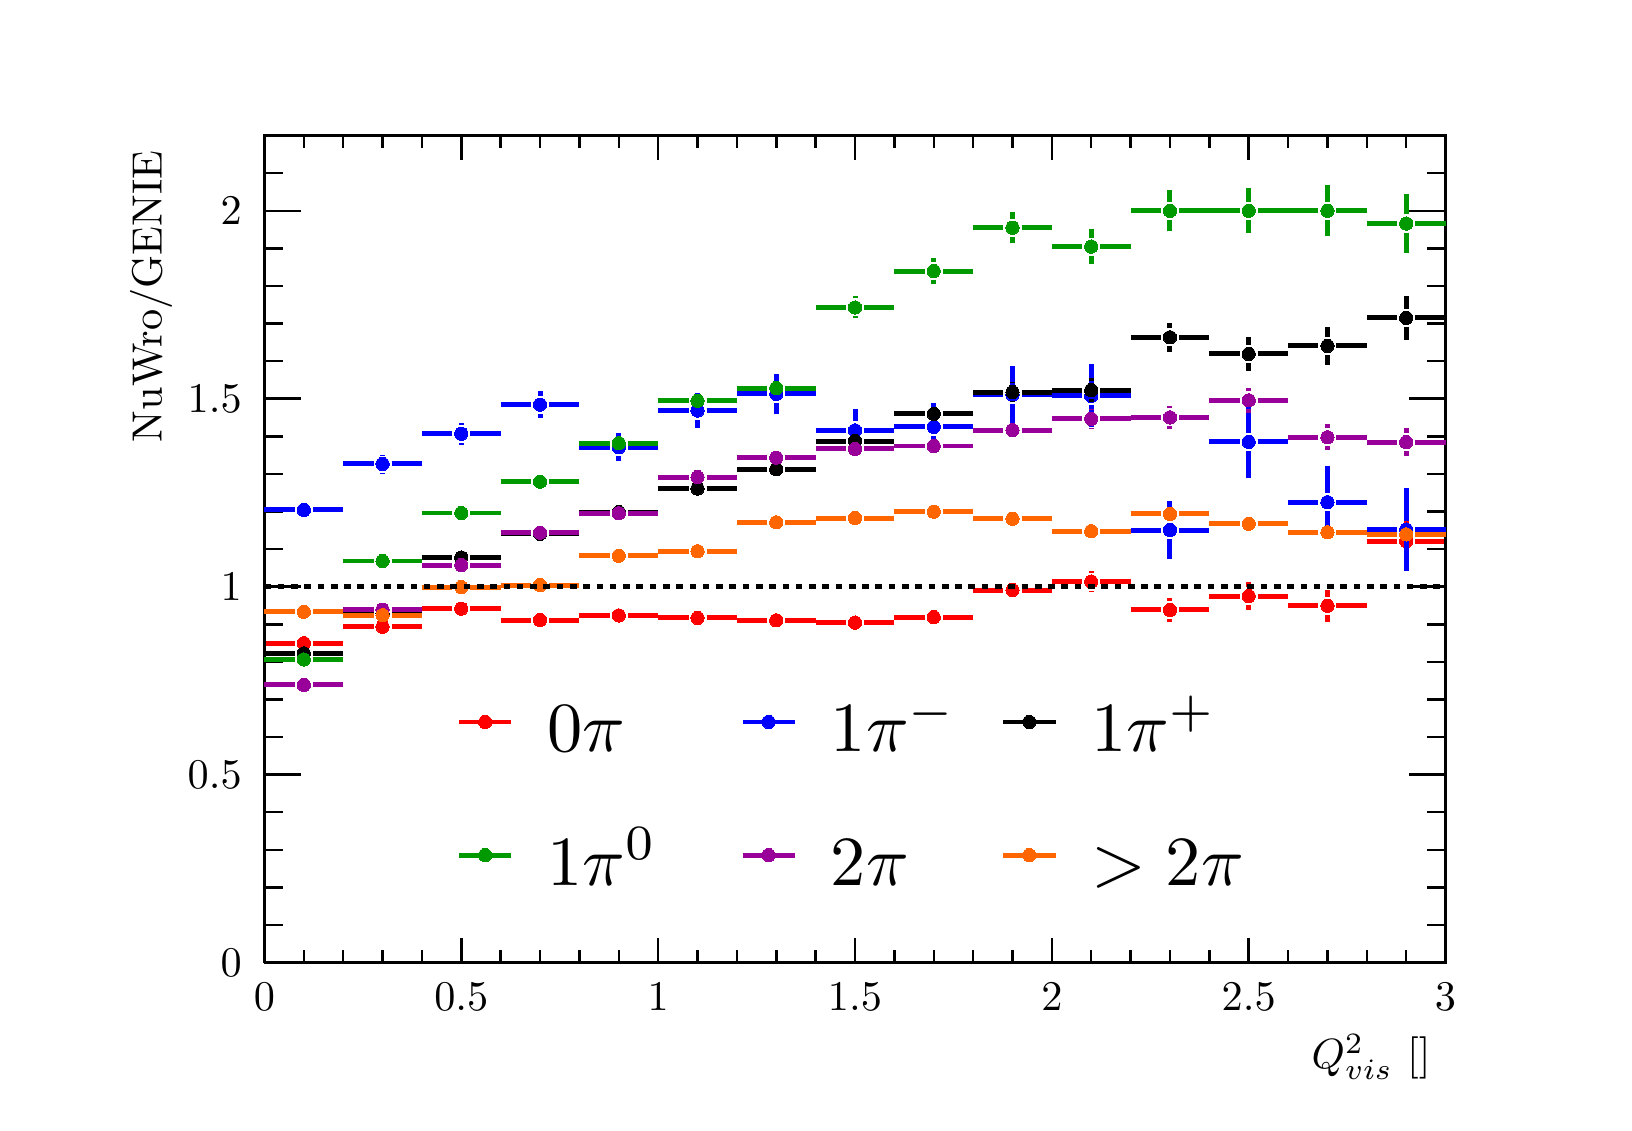
\begin{tikzpicture}
\pgfdeclareplotmark{cross} {
\pgfpathmoveto{\pgfpoint{-0.3\pgfplotmarksize}{\pgfplotmarksize}}
\pgfpathlineto{\pgfpoint{+0.3\pgfplotmarksize}{\pgfplotmarksize}}
\pgfpathlineto{\pgfpoint{+0.3\pgfplotmarksize}{0.3\pgfplotmarksize}}
\pgfpathlineto{\pgfpoint{+1\pgfplotmarksize}{0.3\pgfplotmarksize}}
\pgfpathlineto{\pgfpoint{+1\pgfplotmarksize}{-0.3\pgfplotmarksize}}
\pgfpathlineto{\pgfpoint{+0.3\pgfplotmarksize}{-0.3\pgfplotmarksize}}
\pgfpathlineto{\pgfpoint{+0.3\pgfplotmarksize}{-1.\pgfplotmarksize}}
\pgfpathlineto{\pgfpoint{-0.3\pgfplotmarksize}{-1.\pgfplotmarksize}}
\pgfpathlineto{\pgfpoint{-0.3\pgfplotmarksize}{-0.3\pgfplotmarksize}}
\pgfpathlineto{\pgfpoint{-1.\pgfplotmarksize}{-0.3\pgfplotmarksize}}
\pgfpathlineto{\pgfpoint{-1.\pgfplotmarksize}{0.3\pgfplotmarksize}}
\pgfpathlineto{\pgfpoint{-0.3\pgfplotmarksize}{0.3\pgfplotmarksize}}
\pgfpathclose
\pgfusepathqstroke
}
\pgfdeclareplotmark{cross*} {
\pgfpathmoveto{\pgfpoint{-0.3\pgfplotmarksize}{\pgfplotmarksize}}
\pgfpathlineto{\pgfpoint{+0.3\pgfplotmarksize}{\pgfplotmarksize}}
\pgfpathlineto{\pgfpoint{+0.3\pgfplotmarksize}{0.3\pgfplotmarksize}}
\pgfpathlineto{\pgfpoint{+1\pgfplotmarksize}{0.3\pgfplotmarksize}}
\pgfpathlineto{\pgfpoint{+1\pgfplotmarksize}{-0.3\pgfplotmarksize}}
\pgfpathlineto{\pgfpoint{+0.3\pgfplotmarksize}{-0.3\pgfplotmarksize}}
\pgfpathlineto{\pgfpoint{+0.3\pgfplotmarksize}{-1.\pgfplotmarksize}}
\pgfpathlineto{\pgfpoint{-0.3\pgfplotmarksize}{-1.\pgfplotmarksize}}
\pgfpathlineto{\pgfpoint{-0.3\pgfplotmarksize}{-0.3\pgfplotmarksize}}
\pgfpathlineto{\pgfpoint{-1.\pgfplotmarksize}{-0.3\pgfplotmarksize}}
\pgfpathlineto{\pgfpoint{-1.\pgfplotmarksize}{0.3\pgfplotmarksize}}
\pgfpathlineto{\pgfpoint{-0.3\pgfplotmarksize}{0.3\pgfplotmarksize}}
\pgfpathclose
\pgfusepathqfillstroke
}
\pgfdeclareplotmark{newstar} {
\pgfpathmoveto{\pgfqpoint{0pt}{\pgfplotmarksize}}
\pgfpathlineto{\pgfqpointpolar{44}{0.5\pgfplotmarksize}}
\pgfpathlineto{\pgfqpointpolar{18}{\pgfplotmarksize}}
\pgfpathlineto{\pgfqpointpolar{-20}{0.5\pgfplotmarksize}}
\pgfpathlineto{\pgfqpointpolar{-54}{\pgfplotmarksize}}
\pgfpathlineto{\pgfqpointpolar{-90}{0.5\pgfplotmarksize}}
\pgfpathlineto{\pgfqpointpolar{234}{\pgfplotmarksize}}
\pgfpathlineto{\pgfqpointpolar{198}{0.5\pgfplotmarksize}}
\pgfpathlineto{\pgfqpointpolar{162}{\pgfplotmarksize}}
\pgfpathlineto{\pgfqpointpolar{134}{0.5\pgfplotmarksize}}
\pgfpathclose
\pgfusepathqstroke
}
\pgfdeclareplotmark{newstar*} {
\pgfpathmoveto{\pgfqpoint{0pt}{\pgfplotmarksize}}
\pgfpathlineto{\pgfqpointpolar{44}{0.5\pgfplotmarksize}}
\pgfpathlineto{\pgfqpointpolar{18}{\pgfplotmarksize}}
\pgfpathlineto{\pgfqpointpolar{-20}{0.5\pgfplotmarksize}}
\pgfpathlineto{\pgfqpointpolar{-54}{\pgfplotmarksize}}
\pgfpathlineto{\pgfqpointpolar{-90}{0.5\pgfplotmarksize}}
\pgfpathlineto{\pgfqpointpolar{234}{\pgfplotmarksize}}
\pgfpathlineto{\pgfqpointpolar{198}{0.5\pgfplotmarksize}}
\pgfpathlineto{\pgfqpointpolar{162}{\pgfplotmarksize}}
\pgfpathlineto{\pgfqpointpolar{134}{0.5\pgfplotmarksize}}
\pgfpathclose
\pgfusepathqfillstroke
}
\definecolor{c}{rgb}{1,1,1};
\draw [color=c, fill=c] (0,0) rectangle (20,13.639);
\draw [color=c, fill=c] (3,1.77307) rectangle (18,12.2751);
\definecolor{c}{rgb}{0,0,0};
\draw [c,line width=0.9] (3,1.77307) -- (3,12.2751) -- (18,12.2751) -- (18,1.77307) -- (3,1.77307);
\definecolor{c}{rgb}{1,1,1};
\draw [color=c, fill=c] (3,1.77307) rectangle (18,12.2751);
\definecolor{c}{rgb}{0,0,0};
\draw [c,line width=0.9] (3,1.77307) -- (3,12.2751) -- (18,12.2751) -- (18,1.77307) -- (3,1.77307);
\definecolor{c}{rgb}{1,0,0};
\draw [c,line width=1.8] (3,5.82886) -- (3.38539,5.82886);
\draw [c,line width=1.8] (3.61461,5.82886) -- (4,5.82886);
\foreach \P in {(3.5,5.82886)}{\draw[mark options={color=c,fill=c},mark size=2.402402pt, line width=0.000000pt, mark=*] plot coordinates {\P};}
\draw [c,line width=1.8] (4,6.03849) -- (4.38539,6.03849);
\draw [c,line width=1.8] (4.61461,6.03849) -- (5,6.03849);
\foreach \P in {(4.5,6.03849)}{\draw[mark options={color=c,fill=c},mark size=2.402402pt, line width=0.000000pt, mark=*] plot coordinates {\P};}
\draw [c,line width=1.8] (5,6.26711) -- (5.38539,6.26711);
\draw [c,line width=1.8] (5.61461,6.26711) -- (6,6.26711);
\foreach \P in {(5.5,6.26711)}{\draw[mark options={color=c,fill=c},mark size=2.402402pt, line width=0.000000pt, mark=*] plot coordinates {\P};}
\draw [c,line width=1.8] (6,6.12288) -- (6.38539,6.12288);
\draw [c,line width=1.8] (6.61461,6.12288) -- (7,6.12288);
\foreach \P in {(6.5,6.12288)}{\draw[mark options={color=c,fill=c},mark size=2.402402pt, line width=0.000000pt, mark=*] plot coordinates {\P};}
\draw [c,line width=1.8] (7,6.18166) -- (7.38539,6.18166);
\draw [c,line width=1.8] (7.61461,6.18166) -- (8,6.18166);
\foreach \P in {(7.5,6.18166)}{\draw[mark options={color=c,fill=c},mark size=2.402402pt, line width=0.000000pt, mark=*] plot coordinates {\P};}
\draw [c,line width=1.8] (8,6.14986) -- (8.38539,6.14986);
\draw [c,line width=1.8] (8.61461,6.14986) -- (9,6.14986);
\foreach \P in {(8.5,6.14986)}{\draw[mark options={color=c,fill=c},mark size=2.402402pt, line width=0.000000pt, mark=*] plot coordinates {\P};}
\draw [c,line width=1.8] (9,6.11908) -- (9.38539,6.11908);
\draw [c,line width=1.8] (9.61461,6.11908) -- (10,6.11908);
\foreach \P in {(9.5,6.11908)}{\draw[mark options={color=c,fill=c},mark size=2.402402pt, line width=0.000000pt, mark=*] plot coordinates {\P};}
\draw [c,line width=1.8] (10,6.08987) -- (10.3854,6.08987);
\draw [c,line width=1.8] (10.6146,6.08987) -- (11,6.08987);
\foreach \P in {(10.5,6.08987)}{\draw[mark options={color=c,fill=c},mark size=2.402402pt, line width=0.000000pt, mark=*] plot coordinates {\P};}
\draw [c,line width=1.8] (11,6.16035) -- (11.3854,6.16035);
\draw [c,line width=1.8] (11.6146,6.16035) -- (12,6.16035);
\foreach \P in {(11.5,6.16035)}{\draw[mark options={color=c,fill=c},mark size=2.402402pt, line width=0.000000pt, mark=*] plot coordinates {\P};}
\draw [c,line width=1.8] (12,6.50381) -- (12.3854,6.50381);
\draw [c,line width=1.8] (12.6146,6.50381) -- (13,6.50381);
\foreach \P in {(12.5,6.50381)}{\draw[mark options={color=c,fill=c},mark size=2.402402pt, line width=0.000000pt, mark=*] plot coordinates {\P};}
\draw [c,line width=1.8] (13.5,6.47964) -- (13.5,6.49613);
\draw [c,line width=1.8] (13.5,6.72535) -- (13.5,6.74184);
\draw [c,line width=1.8] (13,6.61074) -- (13.3854,6.61074);
\draw [c,line width=1.8] (13.6146,6.61074) -- (14,6.61074);
\foreach \P in {(13.5,6.61074)}{\draw[mark options={color=c,fill=c},mark size=2.402402pt, line width=0.000000pt, mark=*] plot coordinates {\P};}
\draw [c,line width=1.8] (14.5,6.10391) -- (14.5,6.13613);
\draw [c,line width=1.8] (14.5,6.36536) -- (14.5,6.39759);
\draw [c,line width=1.8] (14,6.25075) -- (14.3854,6.25075);
\draw [c,line width=1.8] (14.6146,6.25075) -- (15,6.25075);
\foreach \P in {(14.5,6.25075)}{\draw[mark options={color=c,fill=c},mark size=2.402402pt, line width=0.000000pt, mark=*] plot coordinates {\P};}
\draw [c,line width=1.8] (15.5,6.25269) -- (15.5,6.31279);
\draw [c,line width=1.8] (15.5,6.54202) -- (15.5,6.60213);
\draw [c,line width=1.8] (15,6.42741) -- (15.3854,6.42741);
\draw [c,line width=1.8] (15.6146,6.42741) -- (16,6.42741);
\foreach \P in {(15.5,6.42741)}{\draw[mark options={color=c,fill=c},mark size=2.402402pt, line width=0.000000pt, mark=*] plot coordinates {\P};}
\draw [c,line width=1.8] (16.5,6.10359) -- (16.5,6.18975);
\draw [c,line width=1.8] (16.5,6.41898) -- (16.5,6.50514);
\draw [c,line width=1.8] (16,6.30436) -- (16.3854,6.30436);
\draw [c,line width=1.8] (16.6146,6.30436) -- (17,6.30436);
\foreach \P in {(16.5,6.30436)}{\draw[mark options={color=c,fill=c},mark size=2.402402pt, line width=0.000000pt, mark=*] plot coordinates {\P};}
\draw [c,line width=1.8] (17.5,6.87193) -- (17.5,7.01171);
\draw [c,line width=1.8] (17.5,7.24094) -- (17.5,7.38072);
\draw [c,line width=1.8] (17,7.12632) -- (17.3854,7.12632);
\draw [c,line width=1.8] (17.6146,7.12632) -- (18,7.12632);
\foreach \P in {(17.5,7.12632)}{\draw[mark options={color=c,fill=c},mark size=2.402402pt, line width=0.000000pt, mark=*] plot coordinates {\P};}
\definecolor{c}{rgb}{0,0,0};
\draw [c,line width=0.9] (3,1.77307) -- (18,1.77307);
\draw [c,line width=0.9] (3,2.07994) -- (3,1.77307);
\draw [c,line width=0.9] (3.5,1.9265) -- (3.5,1.77307);
\draw [c,line width=0.9] (4,1.9265) -- (4,1.77307);
\draw [c,line width=0.9] (4.5,1.9265) -- (4.5,1.77307);
\draw [c,line width=0.9] (5,1.9265) -- (5,1.77307);
\draw [c,line width=0.9] (5.5,2.07994) -- (5.5,1.77307);
\draw [c,line width=0.9] (6,1.9265) -- (6,1.77307);
\draw [c,line width=0.9] (6.5,1.9265) -- (6.5,1.77307);
\draw [c,line width=0.9] (7,1.9265) -- (7,1.77307);
\draw [c,line width=0.9] (7.5,1.9265) -- (7.5,1.77307);
\draw [c,line width=0.9] (8,2.07994) -- (8,1.77307);
\draw [c,line width=0.9] (8.5,1.9265) -- (8.5,1.77307);
\draw [c,line width=0.9] (9,1.9265) -- (9,1.77307);
\draw [c,line width=0.9] (9.5,1.9265) -- (9.5,1.77307);
\draw [c,line width=0.9] (10,1.9265) -- (10,1.77307);
\draw [c,line width=0.9] (10.5,2.07994) -- (10.5,1.77307);
\draw [c,line width=0.9] (11,1.9265) -- (11,1.77307);
\draw [c,line width=0.9] (11.5,1.9265) -- (11.5,1.77307);
\draw [c,line width=0.9] (12,1.9265) -- (12,1.77307);
\draw [c,line width=0.9] (12.5,1.9265) -- (12.5,1.77307);
\draw [c,line width=0.9] (13,2.07994) -- (13,1.77307);
\draw [c,line width=0.9] (13.5,1.9265) -- (13.5,1.77307);
\draw [c,line width=0.9] (14,1.9265) -- (14,1.77307);
\draw [c,line width=0.9] (14.5,1.9265) -- (14.5,1.77307);
\draw [c,line width=0.9] (15,1.9265) -- (15,1.77307);
\draw [c,line width=0.9] (15.5,2.07994) -- (15.5,1.77307);
\draw [c,line width=0.9] (16,1.9265) -- (16,1.77307);
\draw [c,line width=0.9] (16.5,1.9265) -- (16.5,1.77307);
\draw [c,line width=0.9] (17,1.9265) -- (17,1.77307);
\draw [c,line width=0.9] (17.5,1.9265) -- (17.5,1.77307);
\draw [c,line width=0.9] (18,2.07994) -- (18,1.77307);
\draw [c,line width=0.9] (18,2.07994) -- (18,1.77307);
\draw [anchor=base] (3,1.15931) node[scale=1.52731, color=c, rotate=0]{0};
\draw [anchor=base] (5.5,1.15931) node[scale=1.52731, color=c, rotate=0]{0.5};
\draw [anchor=base] (8,1.15931) node[scale=1.52731, color=c, rotate=0]{1};
\draw [anchor=base] (10.5,1.15931) node[scale=1.52731, color=c, rotate=0]{1.5};
\draw [anchor=base] (13,1.15931) node[scale=1.52731, color=c, rotate=0]{2};
\draw [anchor=base] (15.5,1.15931) node[scale=1.52731, color=c, rotate=0]{2.5};
\draw [anchor=base] (18,1.15931) node[scale=1.52731, color=c, rotate=0]{3};
\draw [anchor= east] (18,0.572837) node[scale=1.52731, color=c, rotate=0]{$Q^{2}_{\text{vis}}$ [\si{\giga\electronvolt\squared}] };
\draw [c,line width=0.9] (3,12.2751) -- (18,12.2751);
\draw [c,line width=0.9] (3,11.9682) -- (3,12.2751);
\draw [c,line width=0.9] (3.5,12.1216) -- (3.5,12.2751);
\draw [c,line width=0.9] (4,12.1216) -- (4,12.2751);
\draw [c,line width=0.9] (4.5,12.1216) -- (4.5,12.2751);
\draw [c,line width=0.9] (5,12.1216) -- (5,12.2751);
\draw [c,line width=0.9] (5.5,11.9682) -- (5.5,12.2751);
\draw [c,line width=0.9] (6,12.1216) -- (6,12.2751);
\draw [c,line width=0.9] (6.5,12.1216) -- (6.5,12.2751);
\draw [c,line width=0.9] (7,12.1216) -- (7,12.2751);
\draw [c,line width=0.9] (7.5,12.1216) -- (7.5,12.2751);
\draw [c,line width=0.9] (8,11.9682) -- (8,12.2751);
\draw [c,line width=0.9] (8.5,12.1216) -- (8.5,12.2751);
\draw [c,line width=0.9] (9,12.1216) -- (9,12.2751);
\draw [c,line width=0.9] (9.5,12.1216) -- (9.5,12.2751);
\draw [c,line width=0.9] (10,12.1216) -- (10,12.2751);
\draw [c,line width=0.9] (10.5,11.9682) -- (10.5,12.2751);
\draw [c,line width=0.9] (11,12.1216) -- (11,12.2751);
\draw [c,line width=0.9] (11.5,12.1216) -- (11.5,12.2751);
\draw [c,line width=0.9] (12,12.1216) -- (12,12.2751);
\draw [c,line width=0.9] (12.5,12.1216) -- (12.5,12.2751);
\draw [c,line width=0.9] (13,11.9682) -- (13,12.2751);
\draw [c,line width=0.9] (13.5,12.1216) -- (13.5,12.2751);
\draw [c,line width=0.9] (14,12.1216) -- (14,12.2751);
\draw [c,line width=0.9] (14.5,12.1216) -- (14.5,12.2751);
\draw [c,line width=0.9] (15,12.1216) -- (15,12.2751);
\draw [c,line width=0.9] (15.5,11.9682) -- (15.5,12.2751);
\draw [c,line width=0.9] (16,12.1216) -- (16,12.2751);
\draw [c,line width=0.9] (16.5,12.1216) -- (16.5,12.2751);
\draw [c,line width=0.9] (17,12.1216) -- (17,12.2751);
\draw [c,line width=0.9] (17.5,12.1216) -- (17.5,12.2751);
\draw [c,line width=0.9] (18,11.9682) -- (18,12.2751);
\draw [c,line width=0.9] (18,11.9682) -- (18,12.2751);
\draw [c,line width=0.9] (3,1.77307) -- (3,12.2751);
\draw [c,line width=0.9] (3.462,1.77307) -- (3,1.77307);
\draw [c,line width=0.9] (3.231,2.25043) -- (3,2.25043);
\draw [c,line width=0.9] (3.231,2.72779) -- (3,2.72779);
\draw [c,line width=0.9] (3.231,3.20516) -- (3,3.20516);
\draw [c,line width=0.9] (3.231,3.68252) -- (3,3.68252);
\draw [c,line width=0.9] (3.462,4.15989) -- (3,4.15989);
\draw [c,line width=0.9] (3.231,4.63725) -- (3,4.63725);
\draw [c,line width=0.9] (3.231,5.11461) -- (3,5.11461);
\draw [c,line width=0.9] (3.231,5.59198) -- (3,5.59198);
\draw [c,line width=0.9] (3.231,6.06934) -- (3,6.06934);
\draw [c,line width=0.9] (3.462,6.5467) -- (3,6.5467);
\draw [c,line width=0.9] (3.231,7.02407) -- (3,7.02407);
\draw [c,line width=0.9] (3.231,7.50143) -- (3,7.50143);
\draw [c,line width=0.9] (3.231,7.9788) -- (3,7.9788);
\draw [c,line width=0.9] (3.231,8.45616) -- (3,8.45616);
\draw [c,line width=0.9] (3.462,8.93352) -- (3,8.93352);
\draw [c,line width=0.9] (3.231,9.41089) -- (3,9.41089);
\draw [c,line width=0.9] (3.231,9.88825) -- (3,9.88825);
\draw [c,line width=0.9] (3.231,10.3656) -- (3,10.3656);
\draw [c,line width=0.9] (3.231,10.843) -- (3,10.843);
\draw [c,line width=0.9] (3.462,11.3203) -- (3,11.3203);
\draw [c,line width=0.9] (3.462,11.3203) -- (3,11.3203);
\draw [c,line width=0.9] (3.231,11.7977) -- (3,11.7977);
\draw [c,line width=0.9] (3.231,12.2751) -- (3,12.2751);
\draw [anchor= east] (2.9,1.77307) node[scale=1.52731, color=c, rotate=0]{0};
\draw [anchor= east] (2.9,4.15989) node[scale=1.52731, color=c, rotate=0]{0.5};
\draw [anchor= east] (2.9,6.5467) node[scale=1.52731, color=c, rotate=0]{1};
\draw [anchor= east] (2.9,8.93352) node[scale=1.52731, color=c, rotate=0]{1.5};
\draw [anchor= east] (2.9,11.3203) node[scale=1.52731, color=c, rotate=0]{2};
\draw [anchor= east] (1.56,12.2751) node[scale=1.52731, color=c, rotate=90]{ NuWro/GENIE};
\draw [c,line width=0.9] (18,1.77307) -- (18,12.2751);
\draw [c,line width=0.9] (17.538,1.77307) -- (18,1.77307);
\draw [c,line width=0.9] (17.769,2.25043) -- (18,2.25043);
\draw [c,line width=0.9] (17.769,2.72779) -- (18,2.72779);
\draw [c,line width=0.9] (17.769,3.20516) -- (18,3.20516);
\draw [c,line width=0.9] (17.769,3.68252) -- (18,3.68252);
\draw [c,line width=0.9] (17.538,4.15989) -- (18,4.15989);
\draw [c,line width=0.9] (17.769,4.63725) -- (18,4.63725);
\draw [c,line width=0.9] (17.769,5.11461) -- (18,5.11461);
\draw [c,line width=0.9] (17.769,5.59198) -- (18,5.59198);
\draw [c,line width=0.9] (17.769,6.06934) -- (18,6.06934);
\draw [c,line width=0.9] (17.538,6.5467) -- (18,6.5467);
\draw [c,line width=0.9] (17.769,7.02407) -- (18,7.02407);
\draw [c,line width=0.9] (17.769,7.50143) -- (18,7.50143);
\draw [c,line width=0.9] (17.769,7.9788) -- (18,7.9788);
\draw [c,line width=0.9] (17.769,8.45616) -- (18,8.45616);
\draw [c,line width=0.9] (17.538,8.93352) -- (18,8.93352);
\draw [c,line width=0.9] (17.769,9.41089) -- (18,9.41089);
\draw [c,line width=0.9] (17.769,9.88825) -- (18,9.88825);
\draw [c,line width=0.9] (17.769,10.3656) -- (18,10.3656);
\draw [c,line width=0.9] (17.769,10.843) -- (18,10.843);
\draw [c,line width=0.9] (17.538,11.3203) -- (18,11.3203);
\draw [c,line width=0.9] (17.538,11.3203) -- (18,11.3203);
\draw [c,line width=0.9] (17.769,11.7977) -- (18,11.7977);
\draw [c,line width=0.9] (17.769,12.2751) -- (18,12.2751);
\definecolor{c}{rgb}{0,0,1};
\draw [c,line width=1.8] (3,7.52061) -- (3.38539,7.52061);
\draw [c,line width=1.8] (3.61461,7.52061) -- (4,7.52061);
\foreach \P in {(3.5,7.52061)}{\draw[mark options={color=c,fill=c},mark size=2.402402pt, line width=0.000000pt, mark=*] plot coordinates {\P};}
\draw [c,line width=1.8] (4.5,7.98956) -- (4.5,7.99026);
\draw [c,line width=1.8] (4.5,8.21949) -- (4.5,8.22019);
\draw [c,line width=1.8] (4,8.10488) -- (4.38539,8.10488);
\draw [c,line width=1.8] (4.61461,8.10488) -- (5,8.10488);
\foreach \P in {(4.5,8.10488)}{\draw[mark options={color=c,fill=c},mark size=2.402402pt, line width=0.000000pt, mark=*] plot coordinates {\P};}
\draw [c,line width=1.8] (5.5,8.3504) -- (5.5,8.37484);
\draw [c,line width=1.8] (5.5,8.60406) -- (5.5,8.6285);
\draw [c,line width=1.8] (5,8.48945) -- (5.38539,8.48945);
\draw [c,line width=1.8] (5.61461,8.48945) -- (6,8.48945);
\foreach \P in {(5.5,8.48945)}{\draw[mark options={color=c,fill=c},mark size=2.402402pt, line width=0.000000pt, mark=*] plot coordinates {\P};}
\draw [c,line width=1.8] (6.5,8.68828) -- (6.5,8.74365);
\draw [c,line width=1.8] (6.5,8.97288) -- (6.5,9.02825);
\draw [c,line width=1.8] (6,8.85826) -- (6.38539,8.85826);
\draw [c,line width=1.8] (6.61461,8.85826) -- (7,8.85826);
\foreach \P in {(6.5,8.85826)}{\draw[mark options={color=c,fill=c},mark size=2.402402pt, line width=0.000000pt, mark=*] plot coordinates {\P};}
\draw [c,line width=1.8] (7.5,8.13763) -- (7.5,8.20169);
\draw [c,line width=1.8] (7.5,8.43091) -- (7.5,8.49497);
\draw [c,line width=1.8] (7,8.3163) -- (7.38539,8.3163);
\draw [c,line width=1.8] (7.61461,8.3163) -- (8,8.3163);
\foreach \P in {(7.5,8.3163)}{\draw[mark options={color=c,fill=c},mark size=2.402402pt, line width=0.000000pt, mark=*] plot coordinates {\P};}
\draw [c,line width=1.8] (8.5,8.56533) -- (8.5,8.66955);
\draw [c,line width=1.8] (8.5,8.89877) -- (8.5,9.00299);
\draw [c,line width=1.8] (8,8.78416) -- (8.38539,8.78416);
\draw [c,line width=1.8] (8.61461,8.78416) -- (9,8.78416);
\foreach \P in {(8.5,8.78416)}{\draw[mark options={color=c,fill=c},mark size=2.402402pt, line width=0.000000pt, mark=*] plot coordinates {\P};}
\draw [c,line width=1.8] (9.5,8.74004) -- (9.5,8.87982);
\draw [c,line width=1.8] (9.5,9.10905) -- (9.5,9.24883);
\draw [c,line width=1.8] (9,8.99443) -- (9.38539,8.99443);
\draw [c,line width=1.8] (9.61461,8.99443) -- (10,8.99443);
\foreach \P in {(9.5,8.99443)}{\draw[mark options={color=c,fill=c},mark size=2.402402pt, line width=0.000000pt, mark=*] plot coordinates {\P};}
\draw [c,line width=1.8] (10.5,8.25734) -- (10.5,8.41721);
\draw [c,line width=1.8] (10.5,8.64643) -- (10.5,8.8063);
\draw [c,line width=1.8] (10,8.53182) -- (10.3854,8.53182);
\draw [c,line width=1.8] (10.6146,8.53182) -- (11,8.53182);
\foreach \P in {(10.5,8.53182)}{\draw[mark options={color=c,fill=c},mark size=2.402402pt, line width=0.000000pt, mark=*] plot coordinates {\P};}
\draw [c,line width=1.8] (11.5,8.2699) -- (11.5,8.46171);
\draw [c,line width=1.8] (11.5,8.69094) -- (11.5,8.88275);
\draw [c,line width=1.8] (11,8.57632) -- (11.3854,8.57632);
\draw [c,line width=1.8] (11.6146,8.57632) -- (12,8.57632);
\foreach \P in {(11.5,8.57632)}{\draw[mark options={color=c,fill=c},mark size=2.402402pt, line width=0.000000pt, mark=*] plot coordinates {\P};}
\draw [c,line width=1.8] (12.5,8.61854) -- (12.5,8.87227);
\draw [c,line width=1.8] (12.5,9.1015) -- (12.5,9.35523);
\draw [c,line width=1.8] (12,8.98688) -- (12.3854,8.98688);
\draw [c,line width=1.8] (12.6146,8.98688) -- (13,8.98688);
\foreach \P in {(12.5,8.98688)}{\draw[mark options={color=c,fill=c},mark size=2.402402pt, line width=0.000000pt, mark=*] plot coordinates {\P};}
\draw [c,line width=1.8] (13.5,8.56917) -- (13.5,8.85412);
\draw [c,line width=1.8] (13.5,9.08334) -- (13.5,9.36829);
\draw [c,line width=1.8] (13,8.96873) -- (13.3854,8.96873);
\draw [c,line width=1.8] (13.6146,8.96873) -- (14,8.96873);
\foreach \P in {(13.5,8.96873)}{\draw[mark options={color=c,fill=c},mark size=2.402402pt, line width=0.000000pt, mark=*] plot coordinates {\P};}
\draw [c,line width=1.8] (14.5,6.89727) -- (14.5,7.15055);
\draw [c,line width=1.8] (14.5,7.37978) -- (14.5,7.63306);
\draw [c,line width=1.8] (14,7.26516) -- (14.3854,7.26516);
\draw [c,line width=1.8] (14.6146,7.26516) -- (15,7.26516);
\foreach \P in {(14.5,7.26516)}{\draw[mark options={color=c,fill=c},mark size=2.402402pt, line width=0.000000pt, mark=*] plot coordinates {\P};}
\draw [c,line width=1.8] (15.5,7.92354) -- (15.5,8.27087);
\draw [c,line width=1.8] (15.5,8.5001) -- (15.5,8.84743);
\draw [c,line width=1.8] (15,8.38549) -- (15.3854,8.38549);
\draw [c,line width=1.8] (15.6146,8.38549) -- (16,8.38549);
\foreach \P in {(15.5,8.38549)}{\draw[mark options={color=c,fill=c},mark size=2.402402pt, line width=0.000000pt, mark=*] plot coordinates {\P};}
\draw [c,line width=1.8] (16.5,7.16342) -- (16.5,7.50513);
\draw [c,line width=1.8] (16.5,7.73436) -- (16.5,8.07607);
\draw [c,line width=1.8] (16,7.61974) -- (16.3854,7.61974);
\draw [c,line width=1.8] (16.6146,7.61974) -- (17,7.61974);
\foreach \P in {(16.5,7.61974)}{\draw[mark options={color=c,fill=c},mark size=2.402402pt, line width=0.000000pt, mark=*] plot coordinates {\P};}
\draw [c,line width=1.8] (17.5,6.74312) -- (17.5,7.15648);
\draw [c,line width=1.8] (17.5,7.38571) -- (17.5,7.79908);
\draw [c,line width=1.8] (17,7.2711) -- (17.3854,7.2711);
\draw [c,line width=1.8] (17.6146,7.2711) -- (18,7.2711);
\foreach \P in {(17.5,7.2711)}{\draw[mark options={color=c,fill=c},mark size=2.402402pt, line width=0.000000pt, mark=*] plot coordinates {\P};}
\definecolor{c}{rgb}{0,0,0};
\draw [c,line width=1.8] (3,5.69971) -- (3.38539,5.69971);
\draw [c,line width=1.8] (3.61461,5.69971) -- (4,5.69971);
\foreach \P in {(3.5,5.69971)}{\draw[mark options={color=c,fill=c},mark size=2.402402pt, line width=0.000000pt, mark=*] plot coordinates {\P};}
\draw [c,line width=1.8] (4,6.20869) -- (4.38539,6.20869);
\draw [c,line width=1.8] (4.61461,6.20869) -- (5,6.20869);
\foreach \P in {(4.5,6.20869)}{\draw[mark options={color=c,fill=c},mark size=2.402402pt, line width=0.000000pt, mark=*] plot coordinates {\P};}
\draw [c,line width=1.8] (5,6.91728) -- (5.38539,6.91728);
\draw [c,line width=1.8] (5.61461,6.91728) -- (6,6.91728);
\foreach \P in {(5.5,6.91728)}{\draw[mark options={color=c,fill=c},mark size=2.402402pt, line width=0.000000pt, mark=*] plot coordinates {\P};}
\draw [c,line width=1.8] (6,7.21845) -- (6.38539,7.21845);
\draw [c,line width=1.8] (6.61461,7.21845) -- (7,7.21845);
\foreach \P in {(6.5,7.21845)}{\draw[mark options={color=c,fill=c},mark size=2.402402pt, line width=0.000000pt, mark=*] plot coordinates {\P};}
\draw [c,line width=1.8] (7,7.49374) -- (7.38539,7.49374);
\draw [c,line width=1.8] (7.61461,7.49374) -- (8,7.49374);
\foreach \P in {(7.5,7.49374)}{\draw[mark options={color=c,fill=c},mark size=2.402402pt, line width=0.000000pt, mark=*] plot coordinates {\P};}
\draw [c,line width=1.8] (8,7.79179) -- (8.38539,7.79179);
\draw [c,line width=1.8] (8.61461,7.79179) -- (9,7.79179);
\foreach \P in {(8.5,7.79179)}{\draw[mark options={color=c,fill=c},mark size=2.402402pt, line width=0.000000pt, mark=*] plot coordinates {\P};}
\draw [c,line width=1.8] (9,8.03695) -- (9.38539,8.03695);
\draw [c,line width=1.8] (9.61461,8.03695) -- (10,8.03695);
\foreach \P in {(9.5,8.03695)}{\draw[mark options={color=c,fill=c},mark size=2.402402pt, line width=0.000000pt, mark=*] plot coordinates {\P};}
\draw [c,line width=1.8] (10,8.3953) -- (10.3854,8.3953);
\draw [c,line width=1.8] (10.6146,8.3953) -- (11,8.3953);
\foreach \P in {(10.5,8.3953)}{\draw[mark options={color=c,fill=c},mark size=2.402402pt, line width=0.000000pt, mark=*] plot coordinates {\P};}
\draw [c,line width=1.8] (11,8.74131) -- (11.3854,8.74131);
\draw [c,line width=1.8] (11.6146,8.74131) -- (12,8.74131);
\foreach \P in {(11.5,8.74131)}{\draw[mark options={color=c,fill=c},mark size=2.402402pt, line width=0.000000pt, mark=*] plot coordinates {\P};}
\draw [c,line width=1.8] (12.5,8.88845) -- (12.5,8.90289);
\draw [c,line width=1.8] (12.5,9.13212) -- (12.5,9.14656);
\draw [c,line width=1.8] (12,9.01751) -- (12.3854,9.01751);
\draw [c,line width=1.8] (12.6146,9.01751) -- (13,9.01751);
\foreach \P in {(12.5,9.01751)}{\draw[mark options={color=c,fill=c},mark size=2.402402pt, line width=0.000000pt, mark=*] plot coordinates {\P};}
\draw [c,line width=1.8] (13.5,8.89535) -- (13.5,8.92859);
\draw [c,line width=1.8] (13.5,9.15782) -- (13.5,9.19107);
\draw [c,line width=1.8] (13,9.04321) -- (13.3854,9.04321);
\draw [c,line width=1.8] (13.6146,9.04321) -- (14,9.04321);
\foreach \P in {(13.5,9.04321)}{\draw[mark options={color=c,fill=c},mark size=2.402402pt, line width=0.000000pt, mark=*] plot coordinates {\P};}
\draw [c,line width=1.8] (14.5,9.52667) -- (14.5,9.59931);
\draw [c,line width=1.8] (14.5,9.82853) -- (14.5,9.90117);
\draw [c,line width=1.8] (14,9.71392) -- (14.3854,9.71392);
\draw [c,line width=1.8] (14.6146,9.71392) -- (15,9.71392);
\foreach \P in {(14.5,9.71392)}{\draw[mark options={color=c,fill=c},mark size=2.402402pt, line width=0.000000pt, mark=*] plot coordinates {\P};}
\draw [c,line width=1.8] (15.5,9.29097) -- (15.5,9.38736);
\draw [c,line width=1.8] (15.5,9.61659) -- (15.5,9.71298);
\draw [c,line width=1.8] (15,9.50198) -- (15.3854,9.50198);
\draw [c,line width=1.8] (15.6146,9.50198) -- (16,9.50198);
\foreach \P in {(15.5,9.50198)}{\draw[mark options={color=c,fill=c},mark size=2.402402pt, line width=0.000000pt, mark=*] plot coordinates {\P};}
\draw [c,line width=1.8] (16.5,9.36249) -- (16.5,9.48996);
\draw [c,line width=1.8] (16.5,9.71919) -- (16.5,9.84666);
\draw [c,line width=1.8] (16,9.60458) -- (16.3854,9.60458);
\draw [c,line width=1.8] (16.6146,9.60458) -- (17,9.60458);
\foreach \P in {(16.5,9.60458)}{\draw[mark options={color=c,fill=c},mark size=2.402402pt, line width=0.000000pt, mark=*] plot coordinates {\P};}
\draw [c,line width=1.8] (17.5,9.67941) -- (17.5,9.84565);
\draw [c,line width=1.8] (17.5,10.0749) -- (17.5,10.2411);
\draw [c,line width=1.8] (17,9.96026) -- (17.3854,9.96026);
\draw [c,line width=1.8] (17.6146,9.96026) -- (18,9.96026);
\foreach \P in {(17.5,9.96026)}{\draw[mark options={color=c,fill=c},mark size=2.402402pt, line width=0.000000pt, mark=*] plot coordinates {\P};}
\definecolor{c}{rgb}{0,0.6,0};
\draw [c,line width=1.8] (3,5.62264) -- (3.38539,5.62264);
\draw [c,line width=1.8] (3.61461,5.62264) -- (4,5.62264);
\foreach \P in {(3.5,5.62264)}{\draw[mark options={color=c,fill=c},mark size=2.402402pt, line width=0.000000pt, mark=*] plot coordinates {\P};}
\draw [c,line width=1.8] (4,6.87259) -- (4.38539,6.87259);
\draw [c,line width=1.8] (4.61461,6.87259) -- (5,6.87259);
\foreach \P in {(4.5,6.87259)}{\draw[mark options={color=c,fill=c},mark size=2.402402pt, line width=0.000000pt, mark=*] plot coordinates {\P};}
\draw [c,line width=1.8] (5,7.48218) -- (5.38539,7.48218);
\draw [c,line width=1.8] (5.61461,7.48218) -- (6,7.48218);
\foreach \P in {(5.5,7.48218)}{\draw[mark options={color=c,fill=c},mark size=2.402402pt, line width=0.000000pt, mark=*] plot coordinates {\P};}
\draw [c,line width=1.8] (6,7.87976) -- (6.38539,7.87976);
\draw [c,line width=1.8] (6.61461,7.87976) -- (7,7.87976);
\foreach \P in {(6.5,7.87976)}{\draw[mark options={color=c,fill=c},mark size=2.402402pt, line width=0.000000pt, mark=*] plot coordinates {\P};}
\draw [c,line width=1.8] (7,8.36921) -- (7.38539,8.36921);
\draw [c,line width=1.8] (7.61461,8.36921) -- (8,8.36921);
\foreach \P in {(7.5,8.36921)}{\draw[mark options={color=c,fill=c},mark size=2.402402pt, line width=0.000000pt, mark=*] plot coordinates {\P};}
\draw [c,line width=1.8] (8,8.90687) -- (8.38539,8.90687);
\draw [c,line width=1.8] (8.61461,8.90687) -- (9,8.90687);
\foreach \P in {(8.5,8.90687)}{\draw[mark options={color=c,fill=c},mark size=2.402402pt, line width=0.000000pt, mark=*] plot coordinates {\P};}
\draw [c,line width=1.8] (9,9.06858) -- (9.38539,9.06858);
\draw [c,line width=1.8] (9.61461,9.06858) -- (10,9.06858);
\foreach \P in {(9.5,9.06858)}{\draw[mark options={color=c,fill=c},mark size=2.402402pt, line width=0.000000pt, mark=*] plot coordinates {\P};}
\draw [c,line width=1.8] (10.5,9.95327) -- (10.5,9.97814);
\draw [c,line width=1.8] (10.5,10.2074) -- (10.5,10.2322);
\draw [c,line width=1.8] (10,10.0928) -- (10.3854,10.0928);
\draw [c,line width=1.8] (10.6146,10.0928) -- (11,10.0928);
\foreach \P in {(10.5,10.0928)}{\draw[mark options={color=c,fill=c},mark size=2.402402pt, line width=0.000000pt, mark=*] plot coordinates {\P};}
\draw [c,line width=1.8] (11.5,10.3892) -- (11.5,10.4409);
\draw [c,line width=1.8] (11.5,10.6701) -- (11.5,10.7218);
\draw [c,line width=1.8] (11,10.5555) -- (11.3854,10.5555);
\draw [c,line width=1.8] (11.6146,10.5555) -- (12,10.5555);
\foreach \P in {(11.5,10.5555)}{\draw[mark options={color=c,fill=c},mark size=2.402402pt, line width=0.000000pt, mark=*] plot coordinates {\P};}
\draw [c,line width=1.8] (12.5,10.9078) -- (12.5,10.9911);
\draw [c,line width=1.8] (12.5,11.2203) -- (12.5,11.3035);
\draw [c,line width=1.8] (12,11.1057) -- (12.3854,11.1057);
\draw [c,line width=1.8] (12.6146,11.1057) -- (13,11.1057);
\foreach \P in {(12.5,11.1057)}{\draw[mark options={color=c,fill=c},mark size=2.402402pt, line width=0.000000pt, mark=*] plot coordinates {\P};}
\draw [c,line width=1.8] (13.5,10.6454) -- (13.5,10.7509);
\draw [c,line width=1.8] (13.5,10.9801) -- (13.5,11.0856);
\draw [c,line width=1.8] (13,10.8655) -- (13.3854,10.8655);
\draw [c,line width=1.8] (13.6146,10.8655) -- (14,10.8655);
\foreach \P in {(13.5,10.8655)}{\draw[mark options={color=c,fill=c},mark size=2.402402pt, line width=0.000000pt, mark=*] plot coordinates {\P};}
\draw [c,line width=1.8] (14.5,11.0575) -- (14.5,11.2057);
\draw [c,line width=1.8] (14.5,11.435) -- (14.5,11.5832);
\draw [c,line width=1.8] (14,11.3203) -- (14.3854,11.3203);
\draw [c,line width=1.8] (14.6146,11.3203) -- (15,11.3203);
\foreach \P in {(14.5,11.3203)}{\draw[mark options={color=c,fill=c},mark size=2.402402pt, line width=0.000000pt, mark=*] plot coordinates {\P};}
\draw [c,line width=1.8] (15.5,11.0321) -- (15.5,11.2057);
\draw [c,line width=1.8] (15.5,11.435) -- (15.5,11.6086);
\draw [c,line width=1.8] (15,11.3203) -- (15.3854,11.3203);
\draw [c,line width=1.8] (15.6146,11.3203) -- (16,11.3203);
\foreach \P in {(15.5,11.3203)}{\draw[mark options={color=c,fill=c},mark size=2.402402pt, line width=0.000000pt, mark=*] plot coordinates {\P};}
\draw [c,line width=1.8] (16.5,10.9954) -- (16.5,11.2057);
\draw [c,line width=1.8] (16.5,11.435) -- (16.5,11.6452);
\draw [c,line width=1.8] (16,11.3203) -- (16.3854,11.3203);
\draw [c,line width=1.8] (16.6146,11.3203) -- (17,11.3203);
\foreach \P in {(16.5,11.3203)}{\draw[mark options={color=c,fill=c},mark size=2.402402pt, line width=0.000000pt, mark=*] plot coordinates {\P};}
\draw [c,line width=1.8] (17.5,10.7898) -- (17.5,11.0441);
\draw [c,line width=1.8] (17.5,11.2733) -- (17.5,11.5276);
\draw [c,line width=1.8] (17,11.1587) -- (17.3854,11.1587);
\draw [c,line width=1.8] (17.6146,11.1587) -- (18,11.1587);
\foreach \P in {(17.5,11.1587)}{\draw[mark options={color=c,fill=c},mark size=2.402402pt, line width=0.000000pt, mark=*] plot coordinates {\P};}
\definecolor{c}{rgb}{0.6,0,0.6};
\draw [c,line width=1.8] (3,5.29803) -- (3.38539,5.29803);
\draw [c,line width=1.8] (3.61461,5.29803) -- (4,5.29803);
\foreach \P in {(3.5,5.29803)}{\draw[mark options={color=c,fill=c},mark size=2.402402pt, line width=0.000000pt, mark=*] plot coordinates {\P};}
\draw [c,line width=1.8] (4,6.25471) -- (4.38539,6.25471);
\draw [c,line width=1.8] (4.61461,6.25471) -- (5,6.25471);
\foreach \P in {(4.5,6.25471)}{\draw[mark options={color=c,fill=c},mark size=2.402402pt, line width=0.000000pt, mark=*] plot coordinates {\P};}
\draw [c,line width=1.8] (5,6.82104) -- (5.38539,6.82104);
\draw [c,line width=1.8] (5.61461,6.82104) -- (6,6.82104);
\foreach \P in {(5.5,6.82104)}{\draw[mark options={color=c,fill=c},mark size=2.402402pt, line width=0.000000pt, mark=*] plot coordinates {\P};}
\draw [c,line width=1.8] (6,7.23176) -- (6.38539,7.23176);
\draw [c,line width=1.8] (6.61461,7.23176) -- (7,7.23176);
\foreach \P in {(6.5,7.23176)}{\draw[mark options={color=c,fill=c},mark size=2.402402pt, line width=0.000000pt, mark=*] plot coordinates {\P};}
\draw [c,line width=1.8] (7,7.47949) -- (7.38539,7.47949);
\draw [c,line width=1.8] (7.61461,7.47949) -- (8,7.47949);
\foreach \P in {(7.5,7.47949)}{\draw[mark options={color=c,fill=c},mark size=2.402402pt, line width=0.000000pt, mark=*] plot coordinates {\P};}
\draw [c,line width=1.8] (8,7.93804) -- (8.38539,7.93804);
\draw [c,line width=1.8] (8.61461,7.93804) -- (9,7.93804);
\foreach \P in {(8.5,7.93804)}{\draw[mark options={color=c,fill=c},mark size=2.402402pt, line width=0.000000pt, mark=*] plot coordinates {\P};}
\draw [c,line width=1.8] (9,8.18466) -- (9.38539,8.18466);
\draw [c,line width=1.8] (9.61461,8.18466) -- (10,8.18466);
\foreach \P in {(9.5,8.18466)}{\draw[mark options={color=c,fill=c},mark size=2.402402pt, line width=0.000000pt, mark=*] plot coordinates {\P};}
\draw [c,line width=1.8] (10,8.29552) -- (10.3854,8.29552);
\draw [c,line width=1.8] (10.6146,8.29552) -- (11,8.29552);
\foreach \P in {(10.5,8.29552)}{\draw[mark options={color=c,fill=c},mark size=2.402402pt, line width=0.000000pt, mark=*] plot coordinates {\P};}
\draw [c,line width=1.8] (11,8.33318) -- (11.3854,8.33318);
\draw [c,line width=1.8] (11.6146,8.33318) -- (12,8.33318);
\foreach \P in {(11.5,8.33318)}{\draw[mark options={color=c,fill=c},mark size=2.402402pt, line width=0.000000pt, mark=*] plot coordinates {\P};}
\draw [c,line width=1.8] (12,8.53473) -- (12.3854,8.53473);
\draw [c,line width=1.8] (12.6146,8.53473) -- (13,8.53473);
\foreach \P in {(12.5,8.53473)}{\draw[mark options={color=c,fill=c},mark size=2.402402pt, line width=0.000000pt, mark=*] plot coordinates {\P};}
\draw [c,line width=1.8] (13.5,8.55267) -- (13.5,8.56346);
\draw [c,line width=1.8] (13.5,8.79269) -- (13.5,8.80349);
\draw [c,line width=1.8] (13,8.67808) -- (13.3854,8.67808);
\draw [c,line width=1.8] (13.6146,8.67808) -- (14,8.67808);
\foreach \P in {(13.5,8.67808)}{\draw[mark options={color=c,fill=c},mark size=2.402402pt, line width=0.000000pt, mark=*] plot coordinates {\P};}
\draw [c,line width=1.8] (14.5,8.5553) -- (14.5,8.58192);
\draw [c,line width=1.8] (14.5,8.81115) -- (14.5,8.83777);
\draw [c,line width=1.8] (14,8.69654) -- (14.3854,8.69654);
\draw [c,line width=1.8] (14.6146,8.69654) -- (15,8.69654);
\foreach \P in {(14.5,8.69654)}{\draw[mark options={color=c,fill=c},mark size=2.402402pt, line width=0.000000pt, mark=*] plot coordinates {\P};}
\draw [c,line width=1.8] (15.5,8.75403) -- (15.5,8.79878);
\draw [c,line width=1.8] (15.5,9.02801) -- (15.5,9.07276);
\draw [c,line width=1.8] (15,8.9134) -- (15.3854,8.9134);
\draw [c,line width=1.8] (15.6146,8.9134) -- (16,8.9134);
\foreach \P in {(15.5,8.9134)}{\draw[mark options={color=c,fill=c},mark size=2.402402pt, line width=0.000000pt, mark=*] plot coordinates {\P};}
\draw [c,line width=1.8] (16.5,8.27974) -- (16.5,8.32909);
\draw [c,line width=1.8] (16.5,8.55832) -- (16.5,8.60766);
\draw [c,line width=1.8] (16,8.4437) -- (16.3854,8.4437);
\draw [c,line width=1.8] (16.6146,8.4437) -- (17,8.4437);
\foreach \P in {(16.5,8.4437)}{\draw[mark options={color=c,fill=c},mark size=2.402402pt, line width=0.000000pt, mark=*] plot coordinates {\P};}
\draw [c,line width=1.8] (17.5,8.20299) -- (17.5,8.26778);
\draw [c,line width=1.8] (17.5,8.497) -- (17.5,8.56178);
\draw [c,line width=1.8] (17,8.38239) -- (17.3854,8.38239);
\draw [c,line width=1.8] (17.6146,8.38239) -- (18,8.38239);
\foreach \P in {(17.5,8.38239)}{\draw[mark options={color=c,fill=c},mark size=2.402402pt, line width=0.000000pt, mark=*] plot coordinates {\P};}
\definecolor{c}{rgb}{1,0.4,0};
\draw [c,line width=1.8] (3,6.22772) -- (3.38539,6.22772);
\draw [c,line width=1.8] (3.61461,6.22772) -- (4,6.22772);
\foreach \P in {(3.5,6.22772)}{\draw[mark options={color=c,fill=c},mark size=2.402402pt, line width=0.000000pt, mark=*] plot coordinates {\P};}
\draw [c,line width=1.8] (4,6.1851) -- (4.38539,6.1851);
\draw [c,line width=1.8] (4.61461,6.1851) -- (5,6.1851);
\foreach \P in {(4.5,6.1851)}{\draw[mark options={color=c,fill=c},mark size=2.402402pt, line width=0.000000pt, mark=*] plot coordinates {\P};}
\draw [c,line width=1.8] (5,6.5416) -- (5.38539,6.5416);
\draw [c,line width=1.8] (5.61461,6.5416) -- (6,6.5416);
\foreach \P in {(5.5,6.5416)}{\draw[mark options={color=c,fill=c},mark size=2.402402pt, line width=0.000000pt, mark=*] plot coordinates {\P};}
\draw [c,line width=1.8] (6,6.56632) -- (6.38539,6.56632);
\draw [c,line width=1.8] (6.61461,6.56632) -- (7,6.56632);
\foreach \P in {(6.5,6.56632)}{\draw[mark options={color=c,fill=c},mark size=2.402402pt, line width=0.000000pt, mark=*] plot coordinates {\P};}
\draw [c,line width=1.8] (7,6.93934) -- (7.38539,6.93934);
\draw [c,line width=1.8] (7.61461,6.93934) -- (8,6.93934);
\foreach \P in {(7.5,6.93934)}{\draw[mark options={color=c,fill=c},mark size=2.402402pt, line width=0.000000pt, mark=*] plot coordinates {\P};}
\draw [c,line width=1.8] (8,6.99683) -- (8.38539,6.99683);
\draw [c,line width=1.8] (8.61461,6.99683) -- (9,6.99683);
\foreach \P in {(8.5,6.99683)}{\draw[mark options={color=c,fill=c},mark size=2.402402pt, line width=0.000000pt, mark=*] plot coordinates {\P};}
\draw [c,line width=1.8] (9,7.36404) -- (9.38539,7.36404);
\draw [c,line width=1.8] (9.61461,7.36404) -- (10,7.36404);
\foreach \P in {(9.5,7.36404)}{\draw[mark options={color=c,fill=c},mark size=2.402402pt, line width=0.000000pt, mark=*] plot coordinates {\P};}
\draw [c,line width=1.8] (10,7.41745) -- (10.3854,7.41745);
\draw [c,line width=1.8] (10.6146,7.41745) -- (11,7.41745);
\foreach \P in {(10.5,7.41745)}{\draw[mark options={color=c,fill=c},mark size=2.402402pt, line width=0.000000pt, mark=*] plot coordinates {\P};}
\draw [c,line width=1.8] (11,7.49879) -- (11.3854,7.49879);
\draw [c,line width=1.8] (11.6146,7.49879) -- (12,7.49879);
\foreach \P in {(11.5,7.49879)}{\draw[mark options={color=c,fill=c},mark size=2.402402pt, line width=0.000000pt, mark=*] plot coordinates {\P};}
\draw [c,line width=1.8] (12,7.40886) -- (12.3854,7.40886);
\draw [c,line width=1.8] (12.6146,7.40886) -- (13,7.40886);
\foreach \P in {(12.5,7.40886)}{\draw[mark options={color=c,fill=c},mark size=2.402402pt, line width=0.000000pt, mark=*] plot coordinates {\P};}
\draw [c,line width=1.8] (13,7.25159) -- (13.3854,7.25159);
\draw [c,line width=1.8] (13.6146,7.25159) -- (14,7.25159);
\foreach \P in {(13.5,7.25159)}{\draw[mark options={color=c,fill=c},mark size=2.402402pt, line width=0.000000pt, mark=*] plot coordinates {\P};}
\draw [c,line width=1.8] (14,7.46979) -- (14.3854,7.46979);
\draw [c,line width=1.8] (14.6146,7.46979) -- (15,7.46979);
\foreach \P in {(14.5,7.46979)}{\draw[mark options={color=c,fill=c},mark size=2.402402pt, line width=0.000000pt, mark=*] plot coordinates {\P};}
\draw [c,line width=1.8] (15,7.34605) -- (15.3854,7.34605);
\draw [c,line width=1.8] (15.6146,7.34605) -- (16,7.34605);
\foreach \P in {(15.5,7.34605)}{\draw[mark options={color=c,fill=c},mark size=2.402402pt, line width=0.000000pt, mark=*] plot coordinates {\P};}
\draw [c,line width=1.8] (16,7.23807) -- (16.3854,7.23807);
\draw [c,line width=1.8] (16.6146,7.23807) -- (17,7.23807);
\foreach \P in {(16.5,7.23807)}{\draw[mark options={color=c,fill=c},mark size=2.402402pt, line width=0.000000pt, mark=*] plot coordinates {\P};}
\draw [c,line width=1.8] (17,7.21094) -- (17.3854,7.21094);
\draw [c,line width=1.8] (17.6146,7.21094) -- (18,7.21094);
\foreach \P in {(17.5,7.21094)}{\draw[mark options={color=c,fill=c},mark size=2.402402pt, line width=0.000000pt, mark=*] plot coordinates {\P};}
\definecolor{c}{rgb}{0,0,0};
\draw [c,dash pattern=on 2.40pt off 2.40pt ,line width=1.8] (3,6.5467) -- (18,6.5467);
\definecolor{c}{rgb}{1,1,1};
\draw [color=c, fill=c] (2,12.8206) rectangle (18,13.5708);
\definecolor{c}{rgb}{0,0,0};
%\draw (10,13.1957) node[scale=1.40004, color=c, rotate=0]{$0\pi$};
\definecolor{c}{rgb}{1,1,1};
\draw [color=c, fill=c] (5.32951,2.29226) rectangle (16.7049,5.67335);
\definecolor{c}{rgb}{0,0,0};
\draw [anchor=base west] (6.27746,4.44771) node[scale=2.54552, color=c, rotate=0]{$0\pi$};
\definecolor{c}{rgb}{1,1,1};
\draw [c, fill=c] (5.4717,4.23639) -- (6.13527,4.23639) -- (6.13527,5.41977) -- (5.4717,5.41977);
\definecolor{c}{rgb}{1,0,0};
\draw [c,line width=1.8] (5.4717,4.82808) -- (6.13527,4.82808);
\foreach \P in {(5.80349,4.82808)}{\draw[mark options={color=c,fill=c},mark size=2.402402pt, line width=0.000000pt, mark=*] plot coordinates {\P};}
\definecolor{c}{rgb}{0,0,0};
\draw [anchor=base west] (9.87709,4.44771) node[scale=2.54552, color=c, rotate=0]{$1\pi^{-}$};
\definecolor{c}{rgb}{1,1,1};
\draw [c, fill=c] (9.07134,4.23639) -- (9.7349,4.23639) -- (9.7349,5.41977) -- (9.07134,5.41977);
\definecolor{c}{rgb}{0,0,1};
\draw [c,line width=1.8] (9.07134,4.82808) -- (9.7349,4.82808);
\foreach \P in {(9.40312,4.82808)}{\draw[mark options={color=c,fill=c},mark size=2.402402pt, line width=0.000000pt, mark=*] plot coordinates {\P};}
\definecolor{c}{rgb}{0,0,0};
\draw [anchor=base west] (13.1885,4.44771) node[scale=2.54552, color=c, rotate=0]{$1\pi^{+}$};
\definecolor{c}{rgb}{1,1,1};
\draw [c, fill=c] (12.3827,4.23639) -- (13.0463,4.23639) -- (13.0463,5.41977) -- (12.3827,5.41977);
\definecolor{c}{rgb}{0,0,0};
\draw [c,line width=1.8] (12.3827,4.82808) -- (13.0463,4.82808);
\foreach \P in {(12.7145,4.82808)}{\draw[mark options={color=c,fill=c},mark size=2.402402pt, line width=0.000000pt, mark=*] plot coordinates {\P};}
\draw [anchor=base west] (6.27746,2.75716) node[scale=2.54552, color=c, rotate=0]{$1\pi^{0}$};
\definecolor{c}{rgb}{1,1,1};
\draw [c, fill=c] (5.4717,2.54585) -- (6.13527,2.54585) -- (6.13527,3.72923) -- (5.4717,3.72923);
\definecolor{c}{rgb}{0,0.6,0};
\draw [c,line width=1.8] (5.4717,3.13754) -- (6.13527,3.13754);
\foreach \P in {(5.80349,3.13754)}{\draw[mark options={color=c,fill=c},mark size=2.402402pt, line width=0.000000pt, mark=*] plot coordinates {\P};}
\definecolor{c}{rgb}{0,0,0};
\draw [anchor=base west] (9.87709,2.75716) node[scale=2.54552, color=c, rotate=0]{$2\pi$};
\definecolor{c}{rgb}{1,1,1};
\draw [c, fill=c] (9.07134,2.54585) -- (9.7349,2.54585) -- (9.7349,3.72923) -- (9.07134,3.72923);
\definecolor{c}{rgb}{0.6,0,0.6};
\draw [c,line width=1.8] (9.07134,3.13754) -- (9.7349,3.13754);
\foreach \P in {(9.40312,3.13754)}{\draw[mark options={color=c,fill=c},mark size=2.402402pt, line width=0.000000pt, mark=*] plot coordinates {\P};}
\definecolor{c}{rgb}{0,0,0};
\draw [anchor=base west] (13.1885,2.75716) node[scale=2.54552, color=c, rotate=0]{$>2\pi$};
\definecolor{c}{rgb}{1,1,1};
\draw [c, fill=c] (12.3827,2.54585) -- (13.0463,2.54585) -- (13.0463,3.72923) -- (12.3827,3.72923);
\definecolor{c}{rgb}{1,0.4,0};
\draw [c,line width=1.8] (12.3827,3.13754) -- (13.0463,3.13754);
\foreach \P in {(12.7145,3.13754)}{\draw[mark options={color=c,fill=c},mark size=2.402402pt, line width=0.000000pt, mark=*] plot coordinates {\P};}
\end{tikzpicture}

 		\end{adjustbox}
 	\end{minipage}
 	\caption[Comparison of NuWro and GENIE in $Q^{2}_{\textrm{vis}}$ for FHC]{Ratio of NuWro to GENIE event rates in ND-GAr as a function of $Q^{2}_{\textrm{vis}}$ with the beam in FHC mode. Left: Reconstructed selection. Right: True selection.}
 	\label{fig:Q2CompFhc}
\end{figure}

\begin{figure}[h]
	\begin{minipage}[t]{.5\linewidth}
		\begin{adjustbox}{max totalsize=\linewidth, center}
			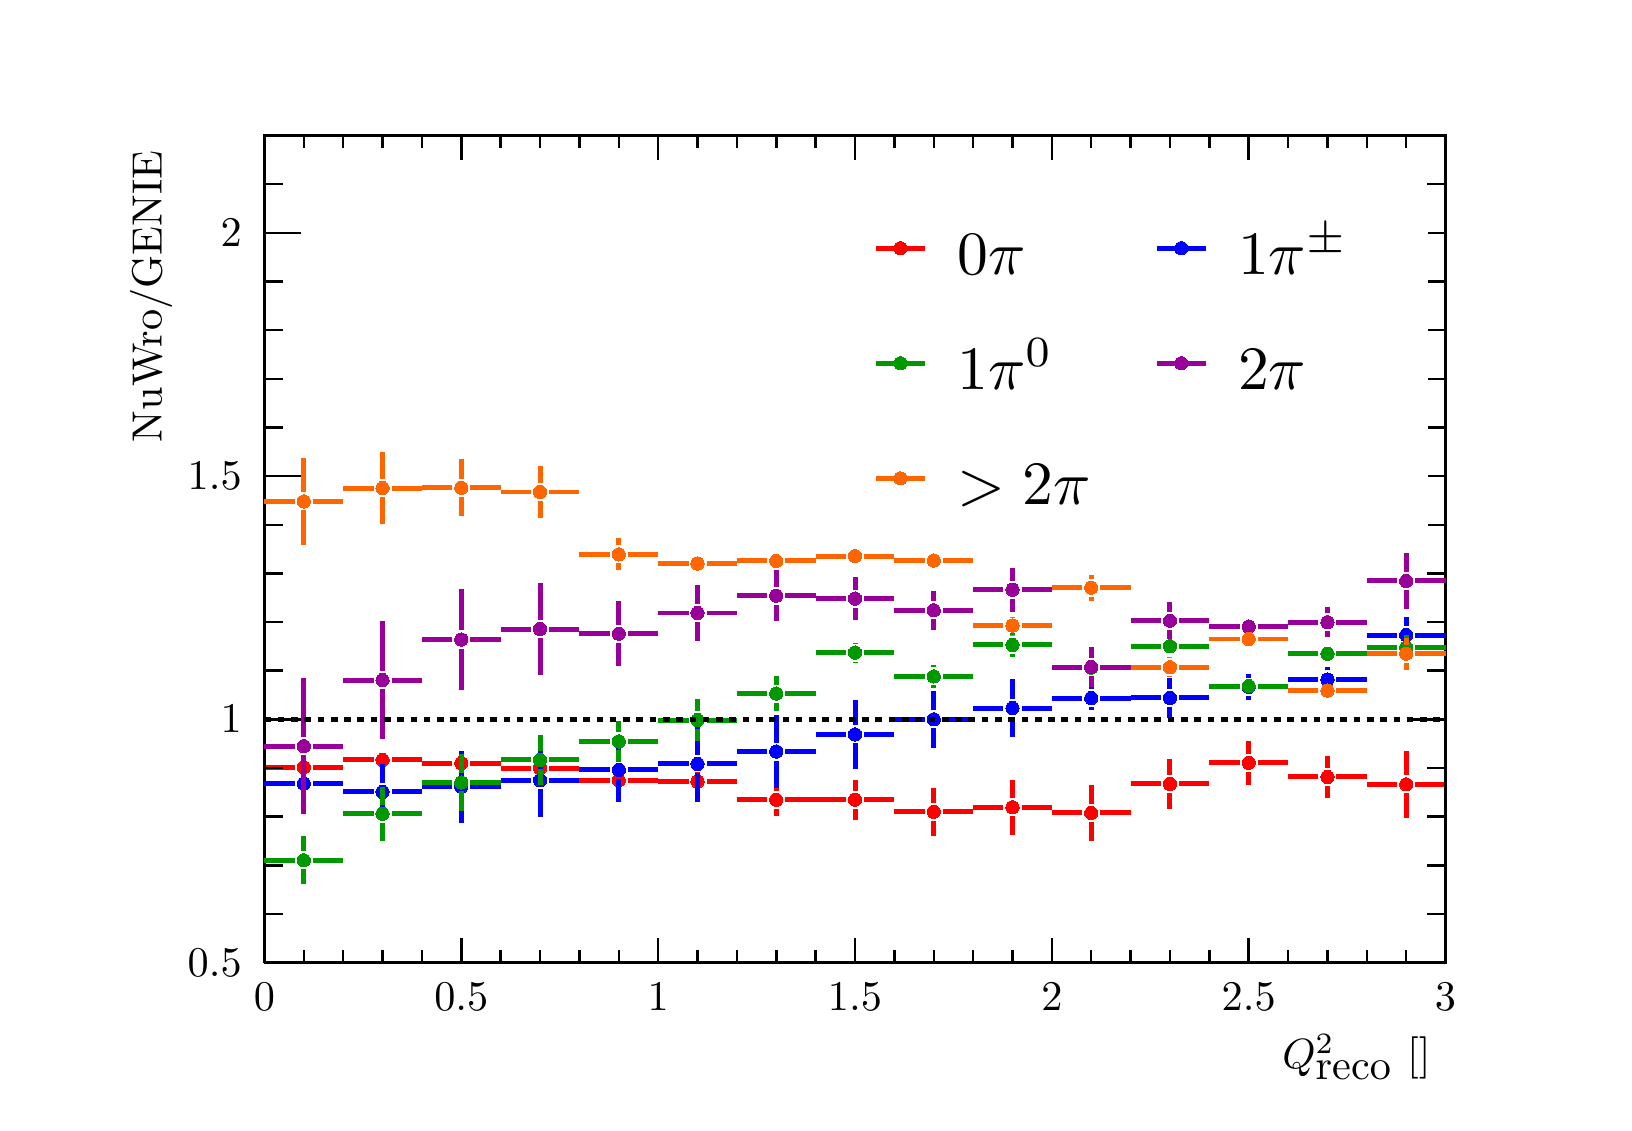
\begin{tikzpicture} 
\pgfdeclareplotmark{cross} {
\pgfpathmoveto{\pgfpoint{-0.3\pgfplotmarksize}{\pgfplotmarksize}}
\pgfpathlineto{\pgfpoint{+0.3\pgfplotmarksize}{\pgfplotmarksize}}
\pgfpathlineto{\pgfpoint{+0.3\pgfplotmarksize}{0.3\pgfplotmarksize}}
\pgfpathlineto{\pgfpoint{+1\pgfplotmarksize}{0.3\pgfplotmarksize}}
\pgfpathlineto{\pgfpoint{+1\pgfplotmarksize}{-0.3\pgfplotmarksize}}
\pgfpathlineto{\pgfpoint{+0.3\pgfplotmarksize}{-0.3\pgfplotmarksize}}
\pgfpathlineto{\pgfpoint{+0.3\pgfplotmarksize}{-1.\pgfplotmarksize}}
\pgfpathlineto{\pgfpoint{-0.3\pgfplotmarksize}{-1.\pgfplotmarksize}}
\pgfpathlineto{\pgfpoint{-0.3\pgfplotmarksize}{-0.3\pgfplotmarksize}}
\pgfpathlineto{\pgfpoint{-1.\pgfplotmarksize}{-0.3\pgfplotmarksize}}
\pgfpathlineto{\pgfpoint{-1.\pgfplotmarksize}{0.3\pgfplotmarksize}}
\pgfpathlineto{\pgfpoint{-0.3\pgfplotmarksize}{0.3\pgfplotmarksize}}
\pgfpathclose
\pgfusepathqstroke
}
\pgfdeclareplotmark{cross*} {
\pgfpathmoveto{\pgfpoint{-0.3\pgfplotmarksize}{\pgfplotmarksize}}
\pgfpathlineto{\pgfpoint{+0.3\pgfplotmarksize}{\pgfplotmarksize}}
\pgfpathlineto{\pgfpoint{+0.3\pgfplotmarksize}{0.3\pgfplotmarksize}}
\pgfpathlineto{\pgfpoint{+1\pgfplotmarksize}{0.3\pgfplotmarksize}}
\pgfpathlineto{\pgfpoint{+1\pgfplotmarksize}{-0.3\pgfplotmarksize}}
\pgfpathlineto{\pgfpoint{+0.3\pgfplotmarksize}{-0.3\pgfplotmarksize}}
\pgfpathlineto{\pgfpoint{+0.3\pgfplotmarksize}{-1.\pgfplotmarksize}}
\pgfpathlineto{\pgfpoint{-0.3\pgfplotmarksize}{-1.\pgfplotmarksize}}
\pgfpathlineto{\pgfpoint{-0.3\pgfplotmarksize}{-0.3\pgfplotmarksize}}
\pgfpathlineto{\pgfpoint{-1.\pgfplotmarksize}{-0.3\pgfplotmarksize}}
\pgfpathlineto{\pgfpoint{-1.\pgfplotmarksize}{0.3\pgfplotmarksize}}
\pgfpathlineto{\pgfpoint{-0.3\pgfplotmarksize}{0.3\pgfplotmarksize}}
\pgfpathclose
\pgfusepathqfillstroke
}
\pgfdeclareplotmark{newstar} {
\pgfpathmoveto{\pgfqpoint{0pt}{\pgfplotmarksize}}
\pgfpathlineto{\pgfqpointpolar{44}{0.5\pgfplotmarksize}}
\pgfpathlineto{\pgfqpointpolar{18}{\pgfplotmarksize}}
\pgfpathlineto{\pgfqpointpolar{-20}{0.5\pgfplotmarksize}}
\pgfpathlineto{\pgfqpointpolar{-54}{\pgfplotmarksize}}
\pgfpathlineto{\pgfqpointpolar{-90}{0.5\pgfplotmarksize}}
\pgfpathlineto{\pgfqpointpolar{234}{\pgfplotmarksize}}
\pgfpathlineto{\pgfqpointpolar{198}{0.5\pgfplotmarksize}}
\pgfpathlineto{\pgfqpointpolar{162}{\pgfplotmarksize}}
\pgfpathlineto{\pgfqpointpolar{134}{0.5\pgfplotmarksize}}
\pgfpathclose
\pgfusepathqstroke
}
\pgfdeclareplotmark{newstar*} {
\pgfpathmoveto{\pgfqpoint{0pt}{\pgfplotmarksize}}
\pgfpathlineto{\pgfqpointpolar{44}{0.5\pgfplotmarksize}}
\pgfpathlineto{\pgfqpointpolar{18}{\pgfplotmarksize}}
\pgfpathlineto{\pgfqpointpolar{-20}{0.5\pgfplotmarksize}}
\pgfpathlineto{\pgfqpointpolar{-54}{\pgfplotmarksize}}
\pgfpathlineto{\pgfqpointpolar{-90}{0.5\pgfplotmarksize}}
\pgfpathlineto{\pgfqpointpolar{234}{\pgfplotmarksize}}
\pgfpathlineto{\pgfqpointpolar{198}{0.5\pgfplotmarksize}}
\pgfpathlineto{\pgfqpointpolar{162}{\pgfplotmarksize}}
\pgfpathlineto{\pgfqpointpolar{134}{0.5\pgfplotmarksize}}
\pgfpathclose
\pgfusepathqfillstroke
}
\definecolor{c}{rgb}{1,1,1};
\draw [color=c, fill=c] (0,0) rectangle (20,13.639);
\draw [color=c, fill=c] (3,1.77307) rectangle (18,12.2751);
\definecolor{c}{rgb}{0,0,0};
\draw [c,line width=0.9] (3,1.77307) -- (3,12.2751) -- (18,12.2751) -- (18,1.77307) -- (3,1.77307);
\definecolor{c}{rgb}{1,1,1};
\draw [color=c, fill=c] (3,1.77307) rectangle (18,12.2751);
\definecolor{c}{rgb}{0,0,0};
\draw [c,line width=0.9] (3,1.77307) -- (3,12.2751) -- (18,12.2751) -- (18,1.77307) -- (3,1.77307);
\definecolor{c}{rgb}{1,0,0};
\draw [c,line width=1.8] (3,4.25421) -- (3.38539,4.25421);
\draw [c,line width=1.8] (3.61461,4.25421) -- (4,4.25421);
\foreach \P in {(3.5,4.25421)}{\draw[mark options={color=c,fill=c},mark size=2.402402pt, line width=0.000000pt, mark=*] plot coordinates {\P};}
\draw [c,line width=1.8] (4,4.34567) -- (4.38539,4.34567);
\draw [c,line width=1.8] (4.61461,4.34567) -- (5,4.34567);
\foreach \P in {(4.5,4.34567)}{\draw[mark options={color=c,fill=c},mark size=2.402402pt, line width=0.000000pt, mark=*] plot coordinates {\P};}
\draw [c,line width=1.8] (5,4.30631) -- (5.38539,4.30631);
\draw [c,line width=1.8] (5.61461,4.30631) -- (6,4.30631);
\foreach \P in {(5.5,4.30631)}{\draw[mark options={color=c,fill=c},mark size=2.402402pt, line width=0.000000pt, mark=*] plot coordinates {\P};}
\draw [c,line width=1.8] (6,4.24171) -- (6.38539,4.24171);
\draw [c,line width=1.8] (6.61461,4.24171) -- (7,4.24171);
\foreach \P in {(6.5,4.24171)}{\draw[mark options={color=c,fill=c},mark size=2.402402pt, line width=0.000000pt, mark=*] plot coordinates {\P};}
\draw [c,line width=1.8] (7,4.08889) -- (7.38539,4.08889);
\draw [c,line width=1.8] (7.61461,4.08889) -- (8,4.08889);
\foreach \P in {(7.5,4.08889)}{\draw[mark options={color=c,fill=c},mark size=2.402402pt, line width=0.000000pt, mark=*] plot coordinates {\P};}
\draw [c,line width=1.8] (8.5,3.95128) -- (8.5,3.95761);
\draw [c,line width=1.8] (8.5,4.18684) -- (8.5,4.19317);
\draw [c,line width=1.8] (8,4.07222) -- (8.38539,4.07222);
\draw [c,line width=1.8] (8.61461,4.07222) -- (9,4.07222);
\foreach \P in {(8.5,4.07222)}{\draw[mark options={color=c,fill=c},mark size=2.402402pt, line width=0.000000pt, mark=*] plot coordinates {\P};}
\draw [c,line width=1.8] (9.5,3.63206) -- (9.5,3.72656);
\draw [c,line width=1.8] (9.5,3.95578) -- (9.5,4.05028);
\draw [c,line width=1.8] (9,3.84117) -- (9.38539,3.84117);
\draw [c,line width=1.8] (9.61461,3.84117) -- (10,3.84117);
\foreach \P in {(9.5,3.84117)}{\draw[mark options={color=c,fill=c},mark size=2.402402pt, line width=0.000000pt, mark=*] plot coordinates {\P};}
\draw [c,line width=1.8] (10.5,3.58793) -- (10.5,3.72697);
\draw [c,line width=1.8] (10.5,3.9562) -- (10.5,4.09523);
\draw [c,line width=1.8] (10,3.84158) -- (10.3854,3.84158);
\draw [c,line width=1.8] (10.6146,3.84158) -- (11,3.84158);
\foreach \P in {(10.5,3.84158)}{\draw[mark options={color=c,fill=c},mark size=2.402402pt, line width=0.000000pt, mark=*] plot coordinates {\P};}
\draw [c,line width=1.8] (11.5,3.38105) -- (11.5,3.57398);
\draw [c,line width=1.8] (11.5,3.8032) -- (11.5,3.99612);
\draw [c,line width=1.8] (11,3.68859) -- (11.3854,3.68859);
\draw [c,line width=1.8] (11.6146,3.68859) -- (12,3.68859);
\foreach \P in {(11.5,3.68859)}{\draw[mark options={color=c,fill=c},mark size=2.402402pt, line width=0.000000pt, mark=*] plot coordinates {\P};}
\draw [c,line width=1.8] (12.5,3.39304) -- (12.5,3.62991);
\draw [c,line width=1.8] (12.5,3.85914) -- (12.5,4.09601);
\draw [c,line width=1.8] (12,3.74452) -- (12.3854,3.74452);
\draw [c,line width=1.8] (12.6146,3.74452) -- (13,3.74452);
\foreach \P in {(12.5,3.74452)}{\draw[mark options={color=c,fill=c},mark size=2.402402pt, line width=0.000000pt, mark=*] plot coordinates {\P};}
\draw [c,line width=1.8] (13.5,3.31572) -- (13.5,3.55841);
\draw [c,line width=1.8] (13.5,3.78764) -- (13.5,4.03034);
\draw [c,line width=1.8] (13,3.67303) -- (13.3854,3.67303);
\draw [c,line width=1.8] (13.6146,3.67303) -- (14,3.67303);
\foreach \P in {(13.5,3.67303)}{\draw[mark options={color=c,fill=c},mark size=2.402402pt, line width=0.000000pt, mark=*] plot coordinates {\P};}
\draw [c,line width=1.8] (14.5,3.72735) -- (14.5,3.92631);
\draw [c,line width=1.8] (14.5,4.15553) -- (14.5,4.35448);
\draw [c,line width=1.8] (14,4.04092) -- (14.3854,4.04092);
\draw [c,line width=1.8] (14.6146,4.04092) -- (15,4.04092);
\foreach \P in {(14.5,4.04092)}{\draw[mark options={color=c,fill=c},mark size=2.402402pt, line width=0.000000pt, mark=*] plot coordinates {\P};}
\draw [c,line width=1.8] (15.5,4.02951) -- (15.5,4.19558);
\draw [c,line width=1.8] (15.5,4.42481) -- (15.5,4.59088);
\draw [c,line width=1.8] (15,4.3102) -- (15.3854,4.3102);
\draw [c,line width=1.8] (15.6146,4.3102) -- (16,4.3102);
\foreach \P in {(15.5,4.3102)}{\draw[mark options={color=c,fill=c},mark size=2.402402pt, line width=0.000000pt, mark=*] plot coordinates {\P};}
\draw [c,line width=1.8] (16.5,3.85896) -- (16.5,4.01508);
\draw [c,line width=1.8] (16.5,4.24431) -- (16.5,4.40042);
\draw [c,line width=1.8] (16,4.12969) -- (16.3854,4.12969);
\draw [c,line width=1.8] (16.6146,4.12969) -- (17,4.12969);
\foreach \P in {(16.5,4.12969)}{\draw[mark options={color=c,fill=c},mark size=2.402402pt, line width=0.000000pt, mark=*] plot coordinates {\P};}
\draw [c,line width=1.8] (17.5,3.61236) -- (17.5,3.92183);
\draw [c,line width=1.8] (17.5,4.15105) -- (17.5,4.46052);
\draw [c,line width=1.8] (17,4.03644) -- (17.3854,4.03644);
\draw [c,line width=1.8] (17.6146,4.03644) -- (18,4.03644);
\foreach \P in {(17.5,4.03644)}{\draw[mark options={color=c,fill=c},mark size=2.402402pt, line width=0.000000pt, mark=*] plot coordinates {\P};}
\definecolor{c}{rgb}{0,0,0};
\draw [c,line width=0.9] (3,1.77307) -- (18,1.77307);
\draw [c,line width=0.9] (3,2.07994) -- (3,1.77307);
\draw [c,line width=0.9] (3.5,1.9265) -- (3.5,1.77307);
\draw [c,line width=0.9] (4,1.9265) -- (4,1.77307);
\draw [c,line width=0.9] (4.5,1.9265) -- (4.5,1.77307);
\draw [c,line width=0.9] (5,1.9265) -- (5,1.77307);
\draw [c,line width=0.9] (5.5,2.07994) -- (5.5,1.77307);
\draw [c,line width=0.9] (6,1.9265) -- (6,1.77307);
\draw [c,line width=0.9] (6.5,1.9265) -- (6.5,1.77307);
\draw [c,line width=0.9] (7,1.9265) -- (7,1.77307);
\draw [c,line width=0.9] (7.5,1.9265) -- (7.5,1.77307);
\draw [c,line width=0.9] (8,2.07994) -- (8,1.77307);
\draw [c,line width=0.9] (8.5,1.9265) -- (8.5,1.77307);
\draw [c,line width=0.9] (9,1.9265) -- (9,1.77307);
\draw [c,line width=0.9] (9.5,1.9265) -- (9.5,1.77307);
\draw [c,line width=0.9] (10,1.9265) -- (10,1.77307);
\draw [c,line width=0.9] (10.5,2.07994) -- (10.5,1.77307);
\draw [c,line width=0.9] (11,1.9265) -- (11,1.77307);
\draw [c,line width=0.9] (11.5,1.9265) -- (11.5,1.77307);
\draw [c,line width=0.9] (12,1.9265) -- (12,1.77307);
\draw [c,line width=0.9] (12.5,1.9265) -- (12.5,1.77307);
\draw [c,line width=0.9] (13,2.07994) -- (13,1.77307);
\draw [c,line width=0.9] (13.5,1.9265) -- (13.5,1.77307);
\draw [c,line width=0.9] (14,1.9265) -- (14,1.77307);
\draw [c,line width=0.9] (14.5,1.9265) -- (14.5,1.77307);
\draw [c,line width=0.9] (15,1.9265) -- (15,1.77307);
\draw [c,line width=0.9] (15.5,2.07994) -- (15.5,1.77307);
\draw [c,line width=0.9] (16,1.9265) -- (16,1.77307);
\draw [c,line width=0.9] (16.5,1.9265) -- (16.5,1.77307);
\draw [c,line width=0.9] (17,1.9265) -- (17,1.77307);
\draw [c,line width=0.9] (17.5,1.9265) -- (17.5,1.77307);
\draw [c,line width=0.9] (18,2.07994) -- (18,1.77307);
\draw [c,line width=0.9] (18,2.07994) -- (18,1.77307);
\draw [anchor=base] (3,1.15931) node[scale=1.52731, color=c, rotate=0]{0};
\draw [anchor=base] (5.5,1.15931) node[scale=1.52731, color=c, rotate=0]{0.5};
\draw [anchor=base] (8,1.15931) node[scale=1.52731, color=c, rotate=0]{1};
\draw [anchor=base] (10.5,1.15931) node[scale=1.52731, color=c, rotate=0]{1.5};
\draw [anchor=base] (13,1.15931) node[scale=1.52731, color=c, rotate=0]{2};
\draw [anchor=base] (15.5,1.15931) node[scale=1.52731, color=c, rotate=0]{2.5};
\draw [anchor=base] (18,1.15931) node[scale=1.52731, color=c, rotate=0]{3};
\draw [anchor= east] (18,0.572837) node[scale=1.52731, color=c, rotate=0]{$Q^{2}_{\textrm{reco}}$ [\si{\GeV\squared}] };
\draw [c,line width=0.9] (3,12.2751) -- (18,12.2751);
\draw [c,line width=0.9] (3,11.9682) -- (3,12.2751);
\draw [c,line width=0.9] (3.5,12.1216) -- (3.5,12.2751);
\draw [c,line width=0.9] (4,12.1216) -- (4,12.2751);
\draw [c,line width=0.9] (4.5,12.1216) -- (4.5,12.2751);
\draw [c,line width=0.9] (5,12.1216) -- (5,12.2751);
\draw [c,line width=0.9] (5.5,11.9682) -- (5.5,12.2751);
\draw [c,line width=0.9] (6,12.1216) -- (6,12.2751);
\draw [c,line width=0.9] (6.5,12.1216) -- (6.5,12.2751);
\draw [c,line width=0.9] (7,12.1216) -- (7,12.2751);
\draw [c,line width=0.9] (7.5,12.1216) -- (7.5,12.2751);
\draw [c,line width=0.9] (8,11.9682) -- (8,12.2751);
\draw [c,line width=0.9] (8.5,12.1216) -- (8.5,12.2751);
\draw [c,line width=0.9] (9,12.1216) -- (9,12.2751);
\draw [c,line width=0.9] (9.5,12.1216) -- (9.5,12.2751);
\draw [c,line width=0.9] (10,12.1216) -- (10,12.2751);
\draw [c,line width=0.9] (10.5,11.9682) -- (10.5,12.2751);
\draw [c,line width=0.9] (11,12.1216) -- (11,12.2751);
\draw [c,line width=0.9] (11.5,12.1216) -- (11.5,12.2751);
\draw [c,line width=0.9] (12,12.1216) -- (12,12.2751);
\draw [c,line width=0.9] (12.5,12.1216) -- (12.5,12.2751);
\draw [c,line width=0.9] (13,11.9682) -- (13,12.2751);
\draw [c,line width=0.9] (13.5,12.1216) -- (13.5,12.2751);
\draw [c,line width=0.9] (14,12.1216) -- (14,12.2751);
\draw [c,line width=0.9] (14.5,12.1216) -- (14.5,12.2751);
\draw [c,line width=0.9] (15,12.1216) -- (15,12.2751);
\draw [c,line width=0.9] (15.5,11.9682) -- (15.5,12.2751);
\draw [c,line width=0.9] (16,12.1216) -- (16,12.2751);
\draw [c,line width=0.9] (16.5,12.1216) -- (16.5,12.2751);
\draw [c,line width=0.9] (17,12.1216) -- (17,12.2751);
\draw [c,line width=0.9] (17.5,12.1216) -- (17.5,12.2751);
\draw [c,line width=0.9] (18,11.9682) -- (18,12.2751);
\draw [c,line width=0.9] (18,11.9682) -- (18,12.2751);
\draw [c,line width=0.9] (3,1.77307) -- (3,12.2751);
\draw [c,line width=0.9] (3.462,1.77307) -- (3,1.77307);
\draw [c,line width=0.9] (3.231,2.39083) -- (3,2.39083);
\draw [c,line width=0.9] (3.231,3.0086) -- (3,3.0086);
\draw [c,line width=0.9] (3.231,3.62636) -- (3,3.62636);
\draw [c,line width=0.9] (3.231,4.24413) -- (3,4.24413);
\draw [c,line width=0.9] (3.462,4.86189) -- (3,4.86189);
\draw [c,line width=0.9] (3.231,5.47966) -- (3,5.47966);
\draw [c,line width=0.9] (3.231,6.09742) -- (3,6.09742);
\draw [c,line width=0.9] (3.231,6.71519) -- (3,6.71519);
\draw [c,line width=0.9] (3.231,7.33295) -- (3,7.33295);
\draw [c,line width=0.9] (3.462,7.95072) -- (3,7.95072);
\draw [c,line width=0.9] (3.231,8.56848) -- (3,8.56848);
\draw [c,line width=0.9] (3.231,9.18625) -- (3,9.18625);
\draw [c,line width=0.9] (3.231,9.80401) -- (3,9.80401);
\draw [c,line width=0.9] (3.231,10.4218) -- (3,10.4218);
\draw [c,line width=0.9] (3.462,11.0395) -- (3,11.0395);
\draw [c,line width=0.9] (3.462,11.0395) -- (3,11.0395);
\draw [c,line width=0.9] (3.231,11.6573) -- (3,11.6573);
\draw [c,line width=0.9] (3.231,12.2751) -- (3,12.2751);
\draw [anchor= east] (2.9,1.77307) node[scale=1.52731, color=c, rotate=0]{0.5};
\draw [anchor= east] (2.9,4.86189) node[scale=1.52731, color=c, rotate=0]{1};
\draw [anchor= east] (2.9,7.95072) node[scale=1.52731, color=c, rotate=0]{1.5};
\draw [anchor= east] (2.9,11.0395) node[scale=1.52731, color=c, rotate=0]{2};
\draw [anchor= east] (1.56,12.2751) node[scale=1.52731, color=c, rotate=90]{ NuWro/GENIE};
\draw [c,line width=0.9] (18,1.77307) -- (18,12.2751);
\draw [c,line width=0.9] (17.538,1.77307) -- (18,1.77307);
\draw [c,line width=0.9] (17.769,2.39083) -- (18,2.39083);
\draw [c,line width=0.9] (17.769,3.0086) -- (18,3.0086);
\draw [c,line width=0.9] (17.769,3.62636) -- (18,3.62636);
\draw [c,line width=0.9] (17.769,4.24413) -- (18,4.24413);
\draw [c,line width=0.9] (17.538,4.86189) -- (18,4.86189);
\draw [c,line width=0.9] (17.769,5.47966) -- (18,5.47966);
\draw [c,line width=0.9] (17.769,6.09742) -- (18,6.09742);
\draw [c,line width=0.9] (17.769,6.71519) -- (18,6.71519);
\draw [c,line width=0.9] (17.769,7.33295) -- (18,7.33295);
\draw [c,line width=0.9] (17.538,7.95072) -- (18,7.95072);
\draw [c,line width=0.9] (17.769,8.56848) -- (18,8.56848);
\draw [c,line width=0.9] (17.769,9.18625) -- (18,9.18625);
\draw [c,line width=0.9] (17.769,9.80401) -- (18,9.80401);
\draw [c,line width=0.9] (17.769,10.4218) -- (18,10.4218);
\draw [c,line width=0.9] (17.538,11.0395) -- (18,11.0395);
\draw [c,line width=0.9] (17.538,11.0395) -- (18,11.0395);
\draw [c,line width=0.9] (17.769,11.6573) -- (18,11.6573);
\draw [c,line width=0.9] (17.769,12.2751) -- (18,12.2751);
\definecolor{c}{rgb}{0,0,1};
\draw [c,line width=1.8] (3.5,3.85564) -- (3.5,3.93025);
\draw [c,line width=1.8] (3.5,4.15947) -- (3.5,4.23409);
\draw [c,line width=1.8] (3,4.04486) -- (3.38539,4.04486);
\draw [c,line width=1.8] (3.61461,4.04486) -- (4,4.04486);
\foreach \P in {(3.5,4.04486)}{\draw[mark options={color=c,fill=c},mark size=2.402402pt, line width=0.000000pt, mark=*] plot coordinates {\P};}
\draw [c,line width=1.8] (4.5,3.58177) -- (4.5,3.82528);
\draw [c,line width=1.8] (4.5,4.05451) -- (4.5,4.29802);
\draw [c,line width=1.8] (4,3.93989) -- (4.38539,3.93989);
\draw [c,line width=1.8] (4.61461,3.93989) -- (5,3.93989);
\foreach \P in {(4.5,3.93989)}{\draw[mark options={color=c,fill=c},mark size=2.402402pt, line width=0.000000pt, mark=*] plot coordinates {\P};}
\draw [c,line width=1.8] (5.5,3.55128) -- (5.5,3.892);
\draw [c,line width=1.8] (5.5,4.12123) -- (5.5,4.46194);
\draw [c,line width=1.8] (5,4.00661) -- (5.38539,4.00661);
\draw [c,line width=1.8] (5.61461,4.00661) -- (6,4.00661);
\foreach \P in {(5.5,4.00661)}{\draw[mark options={color=c,fill=c},mark size=2.402402pt, line width=0.000000pt, mark=*] plot coordinates {\P};}
\draw [c,line width=1.8] (6.5,3.62757) -- (6.5,3.97413);
\draw [c,line width=1.8] (6.5,4.20336) -- (6.5,4.54993);
\draw [c,line width=1.8] (6,4.08875) -- (6.38539,4.08875);
\draw [c,line width=1.8] (6.61461,4.08875) -- (7,4.08875);
\foreach \P in {(6.5,4.08875)}{\draw[mark options={color=c,fill=c},mark size=2.402402pt, line width=0.000000pt, mark=*] plot coordinates {\P};}
\draw [c,line width=1.8] (7.5,3.81352) -- (7.5,4.10518);
\draw [c,line width=1.8] (7.5,4.3344) -- (7.5,4.62606);
\draw [c,line width=1.8] (7,4.21979) -- (7.38539,4.21979);
\draw [c,line width=1.8] (7.61461,4.21979) -- (8,4.21979);
\foreach \P in {(7.5,4.21979)}{\draw[mark options={color=c,fill=c},mark size=2.402402pt, line width=0.000000pt, mark=*] plot coordinates {\P};}
\draw [c,line width=1.8] (8.5,3.81693) -- (8.5,4.18106);
\draw [c,line width=1.8] (8.5,4.41029) -- (8.5,4.77442);
\draw [c,line width=1.8] (8,4.29568) -- (8.38539,4.29568);
\draw [c,line width=1.8] (8.61461,4.29568) -- (9,4.29568);
\foreach \P in {(8.5,4.29568)}{\draw[mark options={color=c,fill=c},mark size=2.402402pt, line width=0.000000pt, mark=*] plot coordinates {\P};}
\draw [c,line width=1.8] (9.5,3.98934) -- (9.5,4.33832);
\draw [c,line width=1.8] (9.5,4.56755) -- (9.5,4.91652);
\draw [c,line width=1.8] (9,4.45293) -- (9.38539,4.45293);
\draw [c,line width=1.8] (9.61461,4.45293) -- (10,4.45293);
\foreach \P in {(9.5,4.45293)}{\draw[mark options={color=c,fill=c},mark size=2.402402pt, line width=0.000000pt, mark=*] plot coordinates {\P};}
\draw [c,line width=1.8] (10.5,4.23524) -- (10.5,4.55537);
\draw [c,line width=1.8] (10.5,4.7846) -- (10.5,5.10473);
\draw [c,line width=1.8] (10,4.66999) -- (10.3854,4.66999);
\draw [c,line width=1.8] (10.6146,4.66999) -- (11,4.66999);
\foreach \P in {(10.5,4.66999)}{\draw[mark options={color=c,fill=c},mark size=2.402402pt, line width=0.000000pt, mark=*] plot coordinates {\P};}
\draw [c,line width=1.8] (11.5,4.49798) -- (11.5,4.74711);
\draw [c,line width=1.8] (11.5,4.97634) -- (11.5,5.22547);
\draw [c,line width=1.8] (11,4.86172) -- (11.3854,4.86172);
\draw [c,line width=1.8] (11.6146,4.86172) -- (12,4.86172);
\foreach \P in {(11.5,4.86172)}{\draw[mark options={color=c,fill=c},mark size=2.402402pt, line width=0.000000pt, mark=*] plot coordinates {\P};}
\draw [c,line width=1.8] (12.5,4.63848) -- (12.5,4.89032);
\draw [c,line width=1.8] (12.5,5.11954) -- (12.5,5.37138);
\draw [c,line width=1.8] (12,5.00493) -- (12.3854,5.00493);
\draw [c,line width=1.8] (12.6146,5.00493) -- (13,5.00493);
\foreach \P in {(12.5,5.00493)}{\draw[mark options={color=c,fill=c},mark size=2.402402pt, line width=0.000000pt, mark=*] plot coordinates {\P};}
\draw [c,line width=1.8] (13.5,4.97669) -- (13.5,5.01721);
\draw [c,line width=1.8] (13.5,5.24644) -- (13.5,5.28695);
\draw [c,line width=1.8] (13,5.13182) -- (13.3854,5.13182);
\draw [c,line width=1.8] (13.6146,5.13182) -- (14,5.13182);
\foreach \P in {(13.5,5.13182)}{\draw[mark options={color=c,fill=c},mark size=2.402402pt, line width=0.000000pt, mark=*] plot coordinates {\P};}
\draw [c,line width=1.8] (14.5,4.88157) -- (14.5,5.01984);
\draw [c,line width=1.8] (14.5,5.24906) -- (14.5,5.38732);
\draw [c,line width=1.8] (14,5.13445) -- (14.3854,5.13445);
\draw [c,line width=1.8] (14.6146,5.13445) -- (15,5.13445);
\foreach \P in {(14.5,5.13445)}{\draw[mark options={color=c,fill=c},mark size=2.402402pt, line width=0.000000pt, mark=*] plot coordinates {\P};}
\draw [c,line width=1.8] (15.5,5.10808) -- (15.5,5.1601);
\draw [c,line width=1.8] (15.5,5.38933) -- (15.5,5.44135);
\draw [c,line width=1.8] (15,5.27471) -- (15.3854,5.27471);
\draw [c,line width=1.8] (15.6146,5.27471) -- (16,5.27471);
\foreach \P in {(15.5,5.27471)}{\draw[mark options={color=c,fill=c},mark size=2.402402pt, line width=0.000000pt, mark=*] plot coordinates {\P};}
\draw [c,line width=1.8] (16.5,5.2049) -- (16.5,5.25334);
\draw [c,line width=1.8] (16.5,5.48257) -- (16.5,5.531);
\draw [c,line width=1.8] (16,5.36795) -- (16.3854,5.36795);
\draw [c,line width=1.8] (16.6146,5.36795) -- (17,5.36795);
\foreach \P in {(16.5,5.36795)}{\draw[mark options={color=c,fill=c},mark size=2.402402pt, line width=0.000000pt, mark=*] plot coordinates {\P};}
\draw [c,line width=1.8] (17.5,5.70018) -- (17.5,5.81797);
\draw [c,line width=1.8] (17.5,6.0472) -- (17.5,6.16499);
\draw [c,line width=1.8] (17,5.93258) -- (17.3854,5.93258);
\draw [c,line width=1.8] (17.6146,5.93258) -- (18,5.93258);
\foreach \P in {(17.5,5.93258)}{\draw[mark options={color=c,fill=c},mark size=2.402402pt, line width=0.000000pt, mark=*] plot coordinates {\P};}
\definecolor{c}{rgb}{0,0.6,0};
\draw [c,line width=1.8] (3.5,2.76788) -- (3.5,2.95756);
\draw [c,line width=1.8] (3.5,3.18679) -- (3.5,3.37647);
\draw [c,line width=1.8] (3,3.07217) -- (3.38539,3.07217);
\draw [c,line width=1.8] (3.61461,3.07217) -- (4,3.07217);
\foreach \P in {(3.5,3.07217)}{\draw[mark options={color=c,fill=c},mark size=2.402402pt, line width=0.000000pt, mark=*] plot coordinates {\P};}
\draw [c,line width=1.8] (4.5,3.32244) -- (4.5,3.54829);
\draw [c,line width=1.8] (4.5,3.77752) -- (4.5,4.00337);
\draw [c,line width=1.8] (4,3.6629) -- (4.38539,3.6629);
\draw [c,line width=1.8] (4.61461,3.6629) -- (5,3.6629);
\foreach \P in {(4.5,3.6629)}{\draw[mark options={color=c,fill=c},mark size=2.402402pt, line width=0.000000pt, mark=*] plot coordinates {\P};}
\draw [c,line width=1.8] (5.5,3.70004) -- (5.5,3.94594);
\draw [c,line width=1.8] (5.5,4.17516) -- (5.5,4.42106);
\draw [c,line width=1.8] (5,4.06055) -- (5.38539,4.06055);
\draw [c,line width=1.8] (5.61461,4.06055) -- (6,4.06055);
\foreach \P in {(5.5,4.06055)}{\draw[mark options={color=c,fill=c},mark size=2.402402pt, line width=0.000000pt, mark=*] plot coordinates {\P};}
\draw [c,line width=1.8] (6.5,4.02444) -- (6.5,4.23098);
\draw [c,line width=1.8] (6.5,4.46021) -- (6.5,4.66675);
\draw [c,line width=1.8] (6,4.3456) -- (6.38539,4.3456);
\draw [c,line width=1.8] (6.61461,4.3456) -- (7,4.3456);
\foreach \P in {(6.5,4.3456)}{\draw[mark options={color=c,fill=c},mark size=2.402402pt, line width=0.000000pt, mark=*] plot coordinates {\P};}
\draw [c,line width=1.8] (7.5,4.3251) -- (7.5,4.46706);
\draw [c,line width=1.8] (7.5,4.69629) -- (7.5,4.83825);
\draw [c,line width=1.8] (7,4.58167) -- (7.38539,4.58167);
\draw [c,line width=1.8] (7.61461,4.58167) -- (8,4.58167);
\foreach \P in {(7.5,4.58167)}{\draw[mark options={color=c,fill=c},mark size=2.402402pt, line width=0.000000pt, mark=*] plot coordinates {\P};}
\draw [c,line width=1.8] (8.5,4.58307) -- (8.5,4.73735);
\draw [c,line width=1.8] (8.5,4.96658) -- (8.5,5.12086);
\draw [c,line width=1.8] (8,4.85196) -- (8.38539,4.85196);
\draw [c,line width=1.8] (8.61461,4.85196) -- (9,4.85196);
\foreach \P in {(8.5,4.85196)}{\draw[mark options={color=c,fill=c},mark size=2.402402pt, line width=0.000000pt, mark=*] plot coordinates {\P};}
\draw [c,line width=1.8] (9.5,4.96684) -- (9.5,5.07409);
\draw [c,line width=1.8] (9.5,5.30332) -- (9.5,5.41058);
\draw [c,line width=1.8] (9,5.18871) -- (9.38539,5.18871);
\draw [c,line width=1.8] (9.61461,5.18871) -- (10,5.18871);
\foreach \P in {(9.5,5.18871)}{\draw[mark options={color=c,fill=c},mark size=2.402402pt, line width=0.000000pt, mark=*] plot coordinates {\P};}
\draw [c,line width=1.8] (10.5,5.58259) -- (10.5,5.59515);
\draw [c,line width=1.8] (10.5,5.82437) -- (10.5,5.83693);
\draw [c,line width=1.8] (10,5.70976) -- (10.3854,5.70976);
\draw [c,line width=1.8] (10.6146,5.70976) -- (11,5.70976);
\foreach \P in {(10.5,5.70976)}{\draw[mark options={color=c,fill=c},mark size=2.402402pt, line width=0.000000pt, mark=*] plot coordinates {\P};}
\draw [c,line width=1.8] (11.5,5.26367) -- (11.5,5.29283);
\draw [c,line width=1.8] (11.5,5.52206) -- (11.5,5.55123);
\draw [c,line width=1.8] (11,5.40745) -- (11.3854,5.40745);
\draw [c,line width=1.8] (11.6146,5.40745) -- (12,5.40745);
\foreach \P in {(11.5,5.40745)}{\draw[mark options={color=c,fill=c},mark size=2.402402pt, line width=0.000000pt, mark=*] plot coordinates {\P};}
\draw [c,line width=1.8] (12.5,5.65917) -- (12.5,5.69177);
\draw [c,line width=1.8] (12.5,5.921) -- (12.5,5.95361);
\draw [c,line width=1.8] (12,5.80639) -- (12.3854,5.80639);
\draw [c,line width=1.8] (12.6146,5.80639) -- (13,5.80639);
\foreach \P in {(12.5,5.80639)}{\draw[mark options={color=c,fill=c},mark size=2.402402pt, line width=0.000000pt, mark=*] plot coordinates {\P};}
\draw [c,line width=1.8] (13,5.51858) -- (13.3854,5.51858);
\draw [c,line width=1.8] (13.6146,5.51858) -- (14,5.51858);
\foreach \P in {(13.5,5.51858)}{\draw[mark options={color=c,fill=c},mark size=2.402402pt, line width=0.000000pt, mark=*] plot coordinates {\P};}
\draw [c,line width=1.8] (14,5.79098) -- (14.3854,5.79098);
\draw [c,line width=1.8] (14.6146,5.79098) -- (15,5.79098);
\foreach \P in {(14.5,5.79098)}{\draw[mark options={color=c,fill=c},mark size=2.402402pt, line width=0.000000pt, mark=*] plot coordinates {\P};}
\draw [c,line width=1.8] (15,5.28459) -- (15.3854,5.28459);
\draw [c,line width=1.8] (15.6146,5.28459) -- (16,5.28459);
\foreach \P in {(15.5,5.28459)}{\draw[mark options={color=c,fill=c},mark size=2.402402pt, line width=0.000000pt, mark=*] plot coordinates {\P};}
\draw [c,line width=1.8] (16,5.6943) -- (16.3854,5.6943);
\draw [c,line width=1.8] (16.6146,5.6943) -- (17,5.6943);
\foreach \P in {(16.5,5.6943)}{\draw[mark options={color=c,fill=c},mark size=2.402402pt, line width=0.000000pt, mark=*] plot coordinates {\P};}
\draw [c,line width=1.8] (17.5,5.61317) -- (17.5,5.65889);
\draw [c,line width=1.8] (17.5,5.88811) -- (17.5,5.93383);
\draw [c,line width=1.8] (17,5.7735) -- (17.3854,5.7735);
\draw [c,line width=1.8] (17.6146,5.7735) -- (18,5.7735);
\foreach \P in {(17.5,5.7735)}{\draw[mark options={color=c,fill=c},mark size=2.402402pt, line width=0.000000pt, mark=*] plot coordinates {\P};}
\definecolor{c}{rgb}{0.6,0,0.6};
\draw [c,line width=1.8] (3.5,3.65904) -- (3.5,4.4065);
\draw [c,line width=1.8] (3.5,4.63573) -- (3.5,5.38318);
\draw [c,line width=1.8] (3,4.52111) -- (3.38539,4.52111);
\draw [c,line width=1.8] (3.61461,4.52111) -- (4,4.52111);
\foreach \P in {(3.5,4.52111)}{\draw[mark options={color=c,fill=c},mark size=2.402402pt, line width=0.000000pt, mark=*] plot coordinates {\P};}
\draw [c,line width=1.8] (4.5,4.60862) -- (4.5,5.24532);
\draw [c,line width=1.8] (4.5,5.47454) -- (4.5,6.11124);
\draw [c,line width=1.8] (4,5.35993) -- (4.38539,5.35993);
\draw [c,line width=1.8] (4.61461,5.35993) -- (5,5.35993);
\foreach \P in {(4.5,5.35993)}{\draw[mark options={color=c,fill=c},mark size=2.402402pt, line width=0.000000pt, mark=*] plot coordinates {\P};}
\draw [c,line width=1.8] (5.5,5.2307) -- (5.5,5.76088);
\draw [c,line width=1.8] (5.5,5.9901) -- (5.5,6.52028);
\draw [c,line width=1.8] (5,5.87549) -- (5.38539,5.87549);
\draw [c,line width=1.8] (5.61461,5.87549) -- (6,5.87549);
\foreach \P in {(5.5,5.87549)}{\draw[mark options={color=c,fill=c},mark size=2.402402pt, line width=0.000000pt, mark=*] plot coordinates {\P};}
\draw [c,line width=1.8] (6.5,5.41876) -- (6.5,5.8942);
\draw [c,line width=1.8] (6.5,6.12343) -- (6.5,6.59886);
\draw [c,line width=1.8] (6,6.00881) -- (6.38539,6.00881);
\draw [c,line width=1.8] (6.61461,6.00881) -- (7,6.00881);
\foreach \P in {(6.5,6.00881)}{\draw[mark options={color=c,fill=c},mark size=2.402402pt, line width=0.000000pt, mark=*] plot coordinates {\P};}
\draw [c,line width=1.8] (7.5,5.53892) -- (7.5,5.83474);
\draw [c,line width=1.8] (7.5,6.06397) -- (7.5,6.3598);
\draw [c,line width=1.8] (7,5.94936) -- (7.38539,5.94936);
\draw [c,line width=1.8] (7.61461,5.94936) -- (8,5.94936);
\foreach \P in {(7.5,5.94936)}{\draw[mark options={color=c,fill=c},mark size=2.402402pt, line width=0.000000pt, mark=*] plot coordinates {\P};}
\draw [c,line width=1.8] (8.5,5.86292) -- (8.5,6.0977);
\draw [c,line width=1.8] (8.5,6.32692) -- (8.5,6.5617);
\draw [c,line width=1.8] (8,6.21231) -- (8.38539,6.21231);
\draw [c,line width=1.8] (8.61461,6.21231) -- (9,6.21231);
\foreach \P in {(8.5,6.21231)}{\draw[mark options={color=c,fill=c},mark size=2.402402pt, line width=0.000000pt, mark=*] plot coordinates {\P};}
\draw [c,line width=1.8] (9.5,6.11151) -- (9.5,6.31766);
\draw [c,line width=1.8] (9.5,6.54689) -- (9.5,6.75304);
\draw [c,line width=1.8] (9,6.43227) -- (9.38539,6.43227);
\draw [c,line width=1.8] (9.61461,6.43227) -- (10,6.43227);
\foreach \P in {(9.5,6.43227)}{\draw[mark options={color=c,fill=c},mark size=2.402402pt, line width=0.000000pt, mark=*] plot coordinates {\P};}
\draw [c,line width=1.8] (10.5,6.11706) -- (10.5,6.28095);
\draw [c,line width=1.8] (10.5,6.51018) -- (10.5,6.67407);
\draw [c,line width=1.8] (10,6.39557) -- (10.3854,6.39557);
\draw [c,line width=1.8] (10.6146,6.39557) -- (11,6.39557);
\foreach \P in {(10.5,6.39557)}{\draw[mark options={color=c,fill=c},mark size=2.402402pt, line width=0.000000pt, mark=*] plot coordinates {\P};}
\draw [c,line width=1.8] (11.5,6.00011) -- (11.5,6.13244);
\draw [c,line width=1.8] (11.5,6.36167) -- (11.5,6.49401);
\draw [c,line width=1.8] (11,6.24706) -- (11.3854,6.24706);
\draw [c,line width=1.8] (11.6146,6.24706) -- (12,6.24706);
\foreach \P in {(11.5,6.24706)}{\draw[mark options={color=c,fill=c},mark size=2.402402pt, line width=0.000000pt, mark=*] plot coordinates {\P};}
\draw [c,line width=1.8] (12.5,6.23056) -- (12.5,6.39411);
\draw [c,line width=1.8] (12.5,6.62333) -- (12.5,6.78688);
\draw [c,line width=1.8] (12,6.50872) -- (12.3854,6.50872);
\draw [c,line width=1.8] (12.6146,6.50872) -- (13,6.50872);
\foreach \P in {(12.5,6.50872)}{\draw[mark options={color=c,fill=c},mark size=2.402402pt, line width=0.000000pt, mark=*] plot coordinates {\P};}
\draw [c,line width=1.8] (13.5,5.27082) -- (13.5,5.4117);
\draw [c,line width=1.8] (13.5,5.64093) -- (13.5,5.78181);
\draw [c,line width=1.8] (13,5.52632) -- (13.3854,5.52632);
\draw [c,line width=1.8] (13.6146,5.52632) -- (14,5.52632);
\foreach \P in {(13.5,5.52632)}{\draw[mark options={color=c,fill=c},mark size=2.402402pt, line width=0.000000pt, mark=*] plot coordinates {\P};}
\draw [c,line width=1.8] (14.5,5.88151) -- (14.5,5.99948);
\draw [c,line width=1.8] (14.5,6.2287) -- (14.5,6.34667);
\draw [c,line width=1.8] (14,6.11409) -- (14.3854,6.11409);
\draw [c,line width=1.8] (14.6146,6.11409) -- (15,6.11409);
\foreach \P in {(14.5,6.11409)}{\draw[mark options={color=c,fill=c},mark size=2.402402pt, line width=0.000000pt, mark=*] plot coordinates {\P};}
\draw [c,line width=1.8] (15,6.03899) -- (15.3854,6.03899);
\draw [c,line width=1.8] (15.6146,6.03899) -- (16,6.03899);
\foreach \P in {(15.5,6.03899)}{\draw[mark options={color=c,fill=c},mark size=2.402402pt, line width=0.000000pt, mark=*] plot coordinates {\P};}
\draw [c,line width=1.8] (16.5,5.90295) -- (16.5,5.97987);
\draw [c,line width=1.8] (16.5,6.2091) -- (16.5,6.28602);
\draw [c,line width=1.8] (16,6.09448) -- (16.3854,6.09448);
\draw [c,line width=1.8] (16.6146,6.09448) -- (17,6.09448);
\foreach \P in {(16.5,6.09448)}{\draw[mark options={color=c,fill=c},mark size=2.402402pt, line width=0.000000pt, mark=*] plot coordinates {\P};}
\draw [c,line width=1.8] (17.5,6.26807) -- (17.5,6.50446);
\draw [c,line width=1.8] (17.5,6.73369) -- (17.5,6.97007);
\draw [c,line width=1.8] (17,6.61907) -- (17.3854,6.61907);
\draw [c,line width=1.8] (17.6146,6.61907) -- (18,6.61907);
\foreach \P in {(17.5,6.61907)}{\draw[mark options={color=c,fill=c},mark size=2.402402pt, line width=0.000000pt, mark=*] plot coordinates {\P};}
\definecolor{c}{rgb}{1,0.4,0};
\draw [c,line width=1.8] (3.5,7.0761) -- (3.5,7.51515);
\draw [c,line width=1.8] (3.5,7.74437) -- (3.5,8.18343);
\draw [c,line width=1.8] (3,7.62976) -- (3.38539,7.62976);
\draw [c,line width=1.8] (3.61461,7.62976) -- (4,7.62976);
\foreach \P in {(3.5,7.62976)}{\draw[mark options={color=c,fill=c},mark size=2.402402pt, line width=0.000000pt, mark=*] plot coordinates {\P};}
\draw [c,line width=1.8] (4.5,7.33943) -- (4.5,7.68486);
\draw [c,line width=1.8] (4.5,7.91409) -- (4.5,8.25952);
\draw [c,line width=1.8] (4,7.79948) -- (4.38539,7.79948);
\draw [c,line width=1.8] (4.61461,7.79948) -- (5,7.79948);
\foreach \P in {(4.5,7.79948)}{\draw[mark options={color=c,fill=c},mark size=2.402402pt, line width=0.000000pt, mark=*] plot coordinates {\P};}
\draw [c,line width=1.8] (5.5,7.43854) -- (5.5,7.68771);
\draw [c,line width=1.8] (5.5,7.91694) -- (5.5,8.16611);
\draw [c,line width=1.8] (5,7.80233) -- (5.38539,7.80233);
\draw [c,line width=1.8] (5.61461,7.80233) -- (6,7.80233);
\foreach \P in {(5.5,7.80233)}{\draw[mark options={color=c,fill=c},mark size=2.402402pt, line width=0.000000pt, mark=*] plot coordinates {\P};}
\draw [c,line width=1.8] (6.5,7.42027) -- (6.5,7.63444);
\draw [c,line width=1.8] (6.5,7.86367) -- (6.5,8.07783);
\draw [c,line width=1.8] (6,7.74905) -- (6.38539,7.74905);
\draw [c,line width=1.8] (6.61461,7.74905) -- (7,7.74905);
\foreach \P in {(6.5,7.74905)}{\draw[mark options={color=c,fill=c},mark size=2.402402pt, line width=0.000000pt, mark=*] plot coordinates {\P};}
\draw [c,line width=1.8] (7.5,6.75391) -- (7.5,6.84229);
\draw [c,line width=1.8] (7.5,7.07151) -- (7.5,7.15989);
\draw [c,line width=1.8] (7,6.9569) -- (7.38539,6.9569);
\draw [c,line width=1.8] (7.61461,6.9569) -- (8,6.9569);
\foreach \P in {(7.5,6.9569)}{\draw[mark options={color=c,fill=c},mark size=2.402402pt, line width=0.000000pt, mark=*] plot coordinates {\P};}
\draw [c,line width=1.8] (8,6.84052) -- (8.38539,6.84052);
\draw [c,line width=1.8] (8.61461,6.84052) -- (9,6.84052);
\foreach \P in {(8.5,6.84052)}{\draw[mark options={color=c,fill=c},mark size=2.402402pt, line width=0.000000pt, mark=*] plot coordinates {\P};}
\draw [c,line width=1.8] (9,6.87444) -- (9.38539,6.87444);
\draw [c,line width=1.8] (9.61461,6.87444) -- (10,6.87444);
\foreach \P in {(9.5,6.87444)}{\draw[mark options={color=c,fill=c},mark size=2.402402pt, line width=0.000000pt, mark=*] plot coordinates {\P};}
\draw [c,line width=1.8] (10,6.93446) -- (10.3854,6.93446);
\draw [c,line width=1.8] (10.6146,6.93446) -- (11,6.93446);
\foreach \P in {(10.5,6.93446)}{\draw[mark options={color=c,fill=c},mark size=2.402402pt, line width=0.000000pt, mark=*] plot coordinates {\P};}
\draw [c,line width=1.8] (11,6.87773) -- (11.3854,6.87773);
\draw [c,line width=1.8] (11.6146,6.87773) -- (12,6.87773);
\foreach \P in {(11.5,6.87773)}{\draw[mark options={color=c,fill=c},mark size=2.402402pt, line width=0.000000pt, mark=*] plot coordinates {\P};}
\draw [c,line width=1.8] (12.5,5.93722) -- (12.5,5.93786);
\draw [c,line width=1.8] (12.5,6.16708) -- (12.5,6.16772);
\draw [c,line width=1.8] (12,6.05247) -- (12.3854,6.05247);
\draw [c,line width=1.8] (12.6146,6.05247) -- (13,6.05247);
\foreach \P in {(12.5,6.05247)}{\draw[mark options={color=c,fill=c},mark size=2.402402pt, line width=0.000000pt, mark=*] plot coordinates {\P};}
\draw [c,line width=1.8] (13.5,6.36843) -- (13.5,6.4196);
\draw [c,line width=1.8] (13.5,6.64883) -- (13.5,6.70001);
\draw [c,line width=1.8] (13,6.53422) -- (13.3854,6.53422);
\draw [c,line width=1.8] (13.6146,6.53422) -- (14,6.53422);
\foreach \P in {(13.5,6.53422)}{\draw[mark options={color=c,fill=c},mark size=2.402402pt, line width=0.000000pt, mark=*] plot coordinates {\P};}
\draw [c,line width=1.8] (14.5,5.39621) -- (14.5,5.40926);
\draw [c,line width=1.8] (14.5,5.63848) -- (14.5,5.65153);
\draw [c,line width=1.8] (14,5.52387) -- (14.3854,5.52387);
\draw [c,line width=1.8] (14.6146,5.52387) -- (15,5.52387);
\foreach \P in {(14.5,5.52387)}{\draw[mark options={color=c,fill=c},mark size=2.402402pt, line width=0.000000pt, mark=*] plot coordinates {\P};}
\draw [c,line width=1.8] (15,5.88208) -- (15.3854,5.88208);
\draw [c,line width=1.8] (15.6146,5.88208) -- (16,5.88208);
\foreach \P in {(15.5,5.88208)}{\draw[mark options={color=c,fill=c},mark size=2.402402pt, line width=0.000000pt, mark=*] plot coordinates {\P};}
\draw [c,line width=1.8] (16,5.22624) -- (16.3854,5.22624);
\draw [c,line width=1.8] (16.6146,5.22624) -- (17,5.22624);
\foreach \P in {(16.5,5.22624)}{\draw[mark options={color=c,fill=c},mark size=2.402402pt, line width=0.000000pt, mark=*] plot coordinates {\P};}
\draw [c,line width=1.8] (17.5,5.49105) -- (17.5,5.58116);
\draw [c,line width=1.8] (17.5,5.81039) -- (17.5,5.9005);
\draw [c,line width=1.8] (17,5.69577) -- (17.3854,5.69577);
\draw [c,line width=1.8] (17.6146,5.69577) -- (18,5.69577);
\foreach \P in {(17.5,5.69577)}{\draw[mark options={color=c,fill=c},mark size=2.402402pt, line width=0.000000pt, mark=*] plot coordinates {\P};}
\definecolor{c}{rgb}{0,0,0};
\draw [c,dash pattern=on 2.40pt off 2.40pt ,line width=1.8] (3,4.86189) -- (18,4.86189);
\definecolor{c}{rgb}{1,1,1};
\draw [color=c, fill=c] (2,12.8206) rectangle (18,13.5708);
\definecolor{c}{rgb}{0,0,0};
%\draw (10,13.1957) node[scale=1.40004, color=c, rotate=0]{$0\pi$};
\definecolor{c}{rgb}{1,1,1};
\draw [color=c, fill=c] (10.6304,7.19198) rectangle (17.765,11.5759);
\definecolor{c}{rgb}{0,0,0};
\draw [anchor=base west] (11.5222,10.5165) node[scale=2.22733, color=c, rotate=0]{$0\pi$};
\definecolor{c}{rgb}{1,1,1};
\draw [c, fill=c] (10.7641,10.3338) -- (11.3884,10.3338) -- (11.3884,11.3567) -- (10.7641,11.3567);
\definecolor{c}{rgb}{1,0,0};
\draw [c,line width=1.8] (10.7641,10.8453) -- (11.3884,10.8453);
\foreach \P in {(11.0763,10.8453)}{\draw[mark options={color=c,fill=c},mark size=2.402402pt, line width=0.000000pt, mark=*] plot coordinates {\P};}
\definecolor{c}{rgb}{0,0,0};
\draw [anchor=base west] (15.0895,10.5165) node[scale=2.22733, color=c, rotate=0]{$1\pi^{\pm}$};
\definecolor{c}{rgb}{1,1,1};
\draw [c, fill=c] (14.3315,10.3338) -- (14.9558,10.3338) -- (14.9558,11.3567) -- (14.3315,11.3567);
\definecolor{c}{rgb}{0,0,1};
\draw [c,line width=1.8] (14.3315,10.8453) -- (14.9558,10.8453);
\foreach \P in {(14.6436,10.8453)}{\draw[mark options={color=c,fill=c},mark size=2.402402pt, line width=0.000000pt, mark=*] plot coordinates {\P};}
\definecolor{c}{rgb}{0,0,0};
\draw [anchor=base west] (11.5222,9.05516) node[scale=2.22733, color=c, rotate=0]{$1\pi^{0}$};
\definecolor{c}{rgb}{1,1,1};
\draw [c, fill=c] (10.7641,8.87249) -- (11.3884,8.87249) -- (11.3884,9.89542) -- (10.7641,9.89542);
\definecolor{c}{rgb}{0,0.6,0};
\draw [c,line width=1.8] (10.7641,9.38395) -- (11.3884,9.38395);
\foreach \P in {(11.0763,9.38395)}{\draw[mark options={color=c,fill=c},mark size=2.402402pt, line width=0.000000pt, mark=*] plot coordinates {\P};}
\definecolor{c}{rgb}{0,0,0};
\draw [anchor=base west] (15.0895,9.05516) node[scale=2.22733, color=c, rotate=0]{$2\pi$};
\definecolor{c}{rgb}{1,1,1};
\draw [c, fill=c] (14.3315,8.87249) -- (14.9558,8.87249) -- (14.9558,9.89542) -- (14.3315,9.89542);
\definecolor{c}{rgb}{0.6,0,0.6};
\draw [c,line width=1.8] (14.3315,9.38395) -- (14.9558,9.38395);
\foreach \P in {(14.6436,9.38395)}{\draw[mark options={color=c,fill=c},mark size=2.402402pt, line width=0.000000pt, mark=*] plot coordinates {\P};}
\definecolor{c}{rgb}{0,0,0};
\draw [anchor=base west] (11.5222,7.59384) node[scale=2.22733, color=c, rotate=0]{$>2\pi$};
\definecolor{c}{rgb}{1,1,1};
\draw [c, fill=c] (10.7641,7.41117) -- (11.3884,7.41117) -- (11.3884,8.4341) -- (10.7641,8.4341);
\definecolor{c}{rgb}{1,0.4,0};
\draw [c,line width=1.8] (10.7641,7.92264) -- (11.3884,7.92264);
\foreach \P in {(11.0763,7.92264)}{\draw[mark options={color=c,fill=c},mark size=2.402402pt, line width=0.000000pt, mark=*] plot coordinates {\P};}
\end{tikzpicture}

		\end{adjustbox}
	\end{minipage}
	\hfill
	\begin{minipage}[t]{.5\linewidth}
		\begin{adjustbox}{max totalsize=\linewidth, center}
			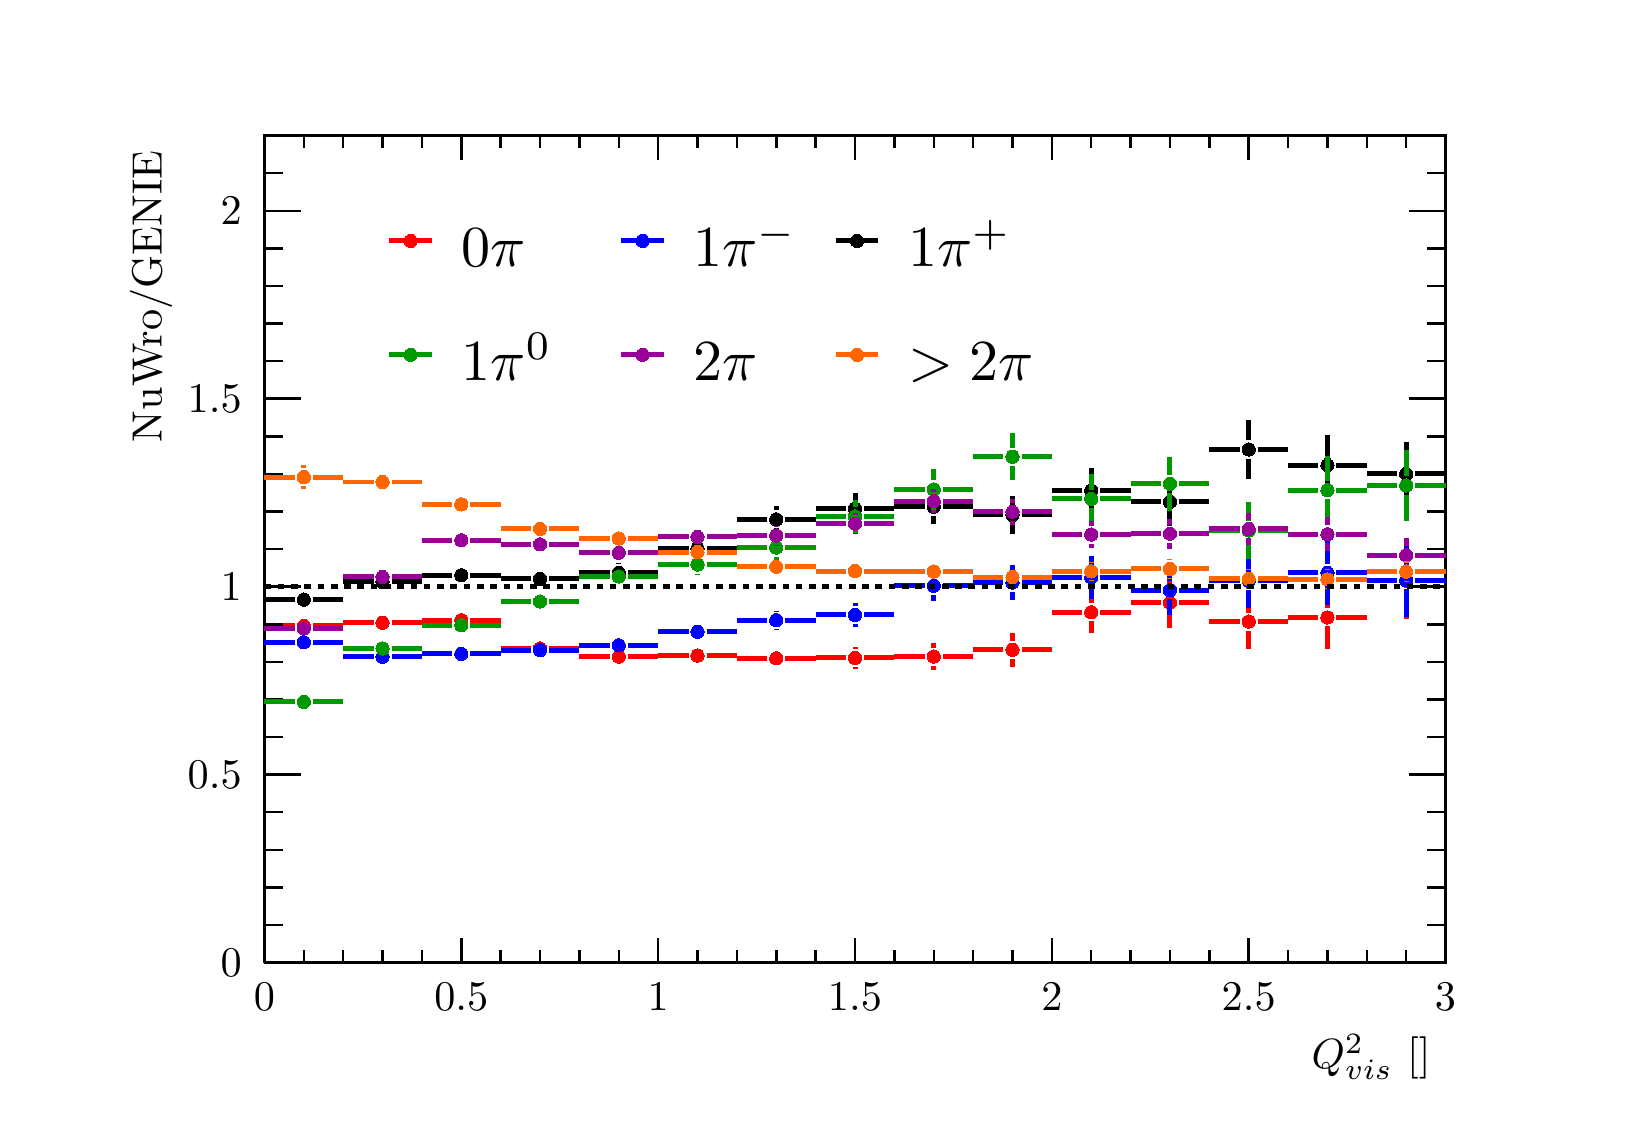
\begin{tikzpicture}
\pgfdeclareplotmark{cross} {
\pgfpathmoveto{\pgfpoint{-0.3\pgfplotmarksize}{\pgfplotmarksize}}
\pgfpathlineto{\pgfpoint{+0.3\pgfplotmarksize}{\pgfplotmarksize}}
\pgfpathlineto{\pgfpoint{+0.3\pgfplotmarksize}{0.3\pgfplotmarksize}}
\pgfpathlineto{\pgfpoint{+1\pgfplotmarksize}{0.3\pgfplotmarksize}}
\pgfpathlineto{\pgfpoint{+1\pgfplotmarksize}{-0.3\pgfplotmarksize}}
\pgfpathlineto{\pgfpoint{+0.3\pgfplotmarksize}{-0.3\pgfplotmarksize}}
\pgfpathlineto{\pgfpoint{+0.3\pgfplotmarksize}{-1.\pgfplotmarksize}}
\pgfpathlineto{\pgfpoint{-0.3\pgfplotmarksize}{-1.\pgfplotmarksize}}
\pgfpathlineto{\pgfpoint{-0.3\pgfplotmarksize}{-0.3\pgfplotmarksize}}
\pgfpathlineto{\pgfpoint{-1.\pgfplotmarksize}{-0.3\pgfplotmarksize}}
\pgfpathlineto{\pgfpoint{-1.\pgfplotmarksize}{0.3\pgfplotmarksize}}
\pgfpathlineto{\pgfpoint{-0.3\pgfplotmarksize}{0.3\pgfplotmarksize}}
\pgfpathclose
\pgfusepathqstroke
}
\pgfdeclareplotmark{cross*} {
\pgfpathmoveto{\pgfpoint{-0.3\pgfplotmarksize}{\pgfplotmarksize}}
\pgfpathlineto{\pgfpoint{+0.3\pgfplotmarksize}{\pgfplotmarksize}}
\pgfpathlineto{\pgfpoint{+0.3\pgfplotmarksize}{0.3\pgfplotmarksize}}
\pgfpathlineto{\pgfpoint{+1\pgfplotmarksize}{0.3\pgfplotmarksize}}
\pgfpathlineto{\pgfpoint{+1\pgfplotmarksize}{-0.3\pgfplotmarksize}}
\pgfpathlineto{\pgfpoint{+0.3\pgfplotmarksize}{-0.3\pgfplotmarksize}}
\pgfpathlineto{\pgfpoint{+0.3\pgfplotmarksize}{-1.\pgfplotmarksize}}
\pgfpathlineto{\pgfpoint{-0.3\pgfplotmarksize}{-1.\pgfplotmarksize}}
\pgfpathlineto{\pgfpoint{-0.3\pgfplotmarksize}{-0.3\pgfplotmarksize}}
\pgfpathlineto{\pgfpoint{-1.\pgfplotmarksize}{-0.3\pgfplotmarksize}}
\pgfpathlineto{\pgfpoint{-1.\pgfplotmarksize}{0.3\pgfplotmarksize}}
\pgfpathlineto{\pgfpoint{-0.3\pgfplotmarksize}{0.3\pgfplotmarksize}}
\pgfpathclose
\pgfusepathqfillstroke
}
\pgfdeclareplotmark{newstar} {
\pgfpathmoveto{\pgfqpoint{0pt}{\pgfplotmarksize}}
\pgfpathlineto{\pgfqpointpolar{44}{0.5\pgfplotmarksize}}
\pgfpathlineto{\pgfqpointpolar{18}{\pgfplotmarksize}}
\pgfpathlineto{\pgfqpointpolar{-20}{0.5\pgfplotmarksize}}
\pgfpathlineto{\pgfqpointpolar{-54}{\pgfplotmarksize}}
\pgfpathlineto{\pgfqpointpolar{-90}{0.5\pgfplotmarksize}}
\pgfpathlineto{\pgfqpointpolar{234}{\pgfplotmarksize}}
\pgfpathlineto{\pgfqpointpolar{198}{0.5\pgfplotmarksize}}
\pgfpathlineto{\pgfqpointpolar{162}{\pgfplotmarksize}}
\pgfpathlineto{\pgfqpointpolar{134}{0.5\pgfplotmarksize}}
\pgfpathclose
\pgfusepathqstroke
}
\pgfdeclareplotmark{newstar*} {
\pgfpathmoveto{\pgfqpoint{0pt}{\pgfplotmarksize}}
\pgfpathlineto{\pgfqpointpolar{44}{0.5\pgfplotmarksize}}
\pgfpathlineto{\pgfqpointpolar{18}{\pgfplotmarksize}}
\pgfpathlineto{\pgfqpointpolar{-20}{0.5\pgfplotmarksize}}
\pgfpathlineto{\pgfqpointpolar{-54}{\pgfplotmarksize}}
\pgfpathlineto{\pgfqpointpolar{-90}{0.5\pgfplotmarksize}}
\pgfpathlineto{\pgfqpointpolar{234}{\pgfplotmarksize}}
\pgfpathlineto{\pgfqpointpolar{198}{0.5\pgfplotmarksize}}
\pgfpathlineto{\pgfqpointpolar{162}{\pgfplotmarksize}}
\pgfpathlineto{\pgfqpointpolar{134}{0.5\pgfplotmarksize}}
\pgfpathclose
\pgfusepathqfillstroke
}
\definecolor{c}{rgb}{1,1,1};
\draw [color=c, fill=c] (0,0) rectangle (20,13.639);
\draw [color=c, fill=c] (3,1.77307) rectangle (18,12.2751);
\definecolor{c}{rgb}{0,0,0};
\draw [c,line width=0.9] (3,1.77307) -- (3,12.2751) -- (18,12.2751) -- (18,1.77307) -- (3,1.77307);
\definecolor{c}{rgb}{1,1,1};
\draw [color=c, fill=c] (3,1.77307) rectangle (18,12.2751);
\definecolor{c}{rgb}{0,0,0};
\draw [c,line width=0.9] (3,1.77307) -- (3,12.2751) -- (18,12.2751) -- (18,1.77307) -- (3,1.77307);
\definecolor{c}{rgb}{1,0,0};
\draw [c,line width=1.8] (3,6.04743) -- (3.38539,6.04743);
\draw [c,line width=1.8] (3.61461,6.04743) -- (4,6.04743);
\foreach \P in {(3.5,6.04743)}{\draw[mark options={color=c,fill=c},mark size=2.402402pt, line width=0.000000pt, mark=*] plot coordinates {\P};}
\draw [c,line width=1.8] (4,6.08852) -- (4.38539,6.08852);
\draw [c,line width=1.8] (4.61461,6.08852) -- (5,6.08852);
\foreach \P in {(4.5,6.08852)}{\draw[mark options={color=c,fill=c},mark size=2.402402pt, line width=0.000000pt, mark=*] plot coordinates {\P};}
\draw [c,line width=1.8] (5,6.12089) -- (5.38539,6.12089);
\draw [c,line width=1.8] (5.61461,6.12089) -- (6,6.12089);
\foreach \P in {(5.5,6.12089)}{\draw[mark options={color=c,fill=c},mark size=2.402402pt, line width=0.000000pt, mark=*] plot coordinates {\P};}
\draw [c,line width=1.8] (6,5.76282) -- (6.38539,5.76282);
\draw [c,line width=1.8] (6.61461,5.76282) -- (7,5.76282);
\foreach \P in {(6.5,5.76282)}{\draw[mark options={color=c,fill=c},mark size=2.402402pt, line width=0.000000pt, mark=*] plot coordinates {\P};}
\draw [c,line width=1.8] (7,5.65759) -- (7.38539,5.65759);
\draw [c,line width=1.8] (7.61461,5.65759) -- (8,5.65759);
\foreach \P in {(7.5,5.65759)}{\draw[mark options={color=c,fill=c},mark size=2.402402pt, line width=0.000000pt, mark=*] plot coordinates {\P};}
\draw [c,line width=1.8] (8,5.6708) -- (8.38539,5.6708);
\draw [c,line width=1.8] (8.61461,5.6708) -- (9,5.6708);
\foreach \P in {(8.5,5.6708)}{\draw[mark options={color=c,fill=c},mark size=2.402402pt, line width=0.000000pt, mark=*] plot coordinates {\P};}
\draw [c,line width=1.8] (9,5.63729) -- (9.38539,5.63729);
\draw [c,line width=1.8] (9.61461,5.63729) -- (10,5.63729);
\foreach \P in {(9.5,5.63729)}{\draw[mark options={color=c,fill=c},mark size=2.402402pt, line width=0.000000pt, mark=*] plot coordinates {\P};}
\draw [c,line width=1.8] (10.5,5.50269) -- (10.5,5.52734);
\draw [c,line width=1.8] (10.5,5.75657) -- (10.5,5.78122);
\draw [c,line width=1.8] (10,5.64196) -- (10.3854,5.64196);
\draw [c,line width=1.8] (10.6146,5.64196) -- (11,5.64196);
\foreach \P in {(10.5,5.64196)}{\draw[mark options={color=c,fill=c},mark size=2.402402pt, line width=0.000000pt, mark=*] plot coordinates {\P};}
\draw [c,line width=1.8] (11.5,5.48713) -- (11.5,5.54456);
\draw [c,line width=1.8] (11.5,5.77379) -- (11.5,5.83122);
\draw [c,line width=1.8] (11,5.65918) -- (11.3854,5.65918);
\draw [c,line width=1.8] (11.6146,5.65918) -- (12,5.65918);
\foreach \P in {(11.5,5.65918)}{\draw[mark options={color=c,fill=c},mark size=2.402402pt, line width=0.000000pt, mark=*] plot coordinates {\P};}
\draw [c,line width=1.8] (12.5,5.53191) -- (12.5,5.63008);
\draw [c,line width=1.8] (12.5,5.8593) -- (12.5,5.95747);
\draw [c,line width=1.8] (12,5.74469) -- (12.3854,5.74469);
\draw [c,line width=1.8] (12.6146,5.74469) -- (13,5.74469);
\foreach \P in {(12.5,5.74469)}{\draw[mark options={color=c,fill=c},mark size=2.402402pt, line width=0.000000pt, mark=*] plot coordinates {\P};}
\draw [c,line width=1.8] (13.5,5.95411) -- (13.5,6.10723);
\draw [c,line width=1.8] (13.5,6.33645) -- (13.5,6.48956);
\draw [c,line width=1.8] (13,6.22184) -- (13.3854,6.22184);
\draw [c,line width=1.8] (13.6146,6.22184) -- (14,6.22184);
\foreach \P in {(13.5,6.22184)}{\draw[mark options={color=c,fill=c},mark size=2.402402pt, line width=0.000000pt, mark=*] plot coordinates {\P};}
\draw [c,line width=1.8] (14.5,6.02788) -- (14.5,6.22779);
\draw [c,line width=1.8] (14.5,6.45701) -- (14.5,6.65692);
\draw [c,line width=1.8] (14,6.3424) -- (14.3854,6.3424);
\draw [c,line width=1.8] (14.6146,6.3424) -- (15,6.3424);
\foreach \P in {(14.5,6.3424)}{\draw[mark options={color=c,fill=c},mark size=2.402402pt, line width=0.000000pt, mark=*] plot coordinates {\P};}
\draw [c,line width=1.8] (15.5,5.75695) -- (15.5,5.98918);
\draw [c,line width=1.8] (15.5,6.21841) -- (15.5,6.45065);
\draw [c,line width=1.8] (15,6.1038) -- (15.3854,6.1038);
\draw [c,line width=1.8] (15.6146,6.1038) -- (16,6.1038);
\foreach \P in {(15.5,6.1038)}{\draw[mark options={color=c,fill=c},mark size=2.402402pt, line width=0.000000pt, mark=*] plot coordinates {\P};}
\draw [c,line width=1.8] (16.5,5.76141) -- (16.5,6.04106);
\draw [c,line width=1.8] (16.5,6.27029) -- (16.5,6.54995);
\draw [c,line width=1.8] (16,6.15568) -- (16.3854,6.15568);
\draw [c,line width=1.8] (16.6146,6.15568) -- (17,6.15568);
\foreach \P in {(16.5,6.15568)}{\draw[mark options={color=c,fill=c},mark size=2.402402pt, line width=0.000000pt, mark=*] plot coordinates {\P};}
\draw [c,line width=1.8] (17.5,6.13333) -- (17.5,6.50904);
\draw [c,line width=1.8] (17.5,6.73827) -- (17.5,7.11399);
\draw [c,line width=1.8] (17,6.62366) -- (17.3854,6.62366);
\draw [c,line width=1.8] (17.6146,6.62366) -- (18,6.62366);
\foreach \P in {(17.5,6.62366)}{\draw[mark options={color=c,fill=c},mark size=2.402402pt, line width=0.000000pt, mark=*] plot coordinates {\P};}
\definecolor{c}{rgb}{0,0,0};
\draw [c,line width=0.9] (3,1.77307) -- (18,1.77307);
\draw [c,line width=0.9] (3,2.07994) -- (3,1.77307);
\draw [c,line width=0.9] (3.5,1.9265) -- (3.5,1.77307);
\draw [c,line width=0.9] (4,1.9265) -- (4,1.77307);
\draw [c,line width=0.9] (4.5,1.9265) -- (4.5,1.77307);
\draw [c,line width=0.9] (5,1.9265) -- (5,1.77307);
\draw [c,line width=0.9] (5.5,2.07994) -- (5.5,1.77307);
\draw [c,line width=0.9] (6,1.9265) -- (6,1.77307);
\draw [c,line width=0.9] (6.5,1.9265) -- (6.5,1.77307);
\draw [c,line width=0.9] (7,1.9265) -- (7,1.77307);
\draw [c,line width=0.9] (7.5,1.9265) -- (7.5,1.77307);
\draw [c,line width=0.9] (8,2.07994) -- (8,1.77307);
\draw [c,line width=0.9] (8.5,1.9265) -- (8.5,1.77307);
\draw [c,line width=0.9] (9,1.9265) -- (9,1.77307);
\draw [c,line width=0.9] (9.5,1.9265) -- (9.5,1.77307);
\draw [c,line width=0.9] (10,1.9265) -- (10,1.77307);
\draw [c,line width=0.9] (10.5,2.07994) -- (10.5,1.77307);
\draw [c,line width=0.9] (11,1.9265) -- (11,1.77307);
\draw [c,line width=0.9] (11.5,1.9265) -- (11.5,1.77307);
\draw [c,line width=0.9] (12,1.9265) -- (12,1.77307);
\draw [c,line width=0.9] (12.5,1.9265) -- (12.5,1.77307);
\draw [c,line width=0.9] (13,2.07994) -- (13,1.77307);
\draw [c,line width=0.9] (13.5,1.9265) -- (13.5,1.77307);
\draw [c,line width=0.9] (14,1.9265) -- (14,1.77307);
\draw [c,line width=0.9] (14.5,1.9265) -- (14.5,1.77307);
\draw [c,line width=0.9] (15,1.9265) -- (15,1.77307);
\draw [c,line width=0.9] (15.5,2.07994) -- (15.5,1.77307);
\draw [c,line width=0.9] (16,1.9265) -- (16,1.77307);
\draw [c,line width=0.9] (16.5,1.9265) -- (16.5,1.77307);
\draw [c,line width=0.9] (17,1.9265) -- (17,1.77307);
\draw [c,line width=0.9] (17.5,1.9265) -- (17.5,1.77307);
\draw [c,line width=0.9] (18,2.07994) -- (18,1.77307);
\draw [c,line width=0.9] (18,2.07994) -- (18,1.77307);
\draw [anchor=base] (3,1.15931) node[scale=1.52731, color=c, rotate=0]{0};
\draw [anchor=base] (5.5,1.15931) node[scale=1.52731, color=c, rotate=0]{0.5};
\draw [anchor=base] (8,1.15931) node[scale=1.52731, color=c, rotate=0]{1};
\draw [anchor=base] (10.5,1.15931) node[scale=1.52731, color=c, rotate=0]{1.5};
\draw [anchor=base] (13,1.15931) node[scale=1.52731, color=c, rotate=0]{2};
\draw [anchor=base] (15.5,1.15931) node[scale=1.52731, color=c, rotate=0]{2.5};
\draw [anchor=base] (18,1.15931) node[scale=1.52731, color=c, rotate=0]{3};
\draw [anchor= east] (18,0.572837) node[scale=1.52731, color=c, rotate=0]{ $Q^{2}_{\text{vis}}$ [\si{\giga\electronvolt\squared}] };
\draw [c,line width=0.9] (3,12.2751) -- (18,12.2751);
\draw [c,line width=0.9] (3,11.9682) -- (3,12.2751);
\draw [c,line width=0.9] (3.5,12.1216) -- (3.5,12.2751);
\draw [c,line width=0.9] (4,12.1216) -- (4,12.2751);
\draw [c,line width=0.9] (4.5,12.1216) -- (4.5,12.2751);
\draw [c,line width=0.9] (5,12.1216) -- (5,12.2751);
\draw [c,line width=0.9] (5.5,11.9682) -- (5.5,12.2751);
\draw [c,line width=0.9] (6,12.1216) -- (6,12.2751);
\draw [c,line width=0.9] (6.5,12.1216) -- (6.5,12.2751);
\draw [c,line width=0.9] (7,12.1216) -- (7,12.2751);
\draw [c,line width=0.9] (7.5,12.1216) -- (7.5,12.2751);
\draw [c,line width=0.9] (8,11.9682) -- (8,12.2751);
\draw [c,line width=0.9] (8.5,12.1216) -- (8.5,12.2751);
\draw [c,line width=0.9] (9,12.1216) -- (9,12.2751);
\draw [c,line width=0.9] (9.5,12.1216) -- (9.5,12.2751);
\draw [c,line width=0.9] (10,12.1216) -- (10,12.2751);
\draw [c,line width=0.9] (10.5,11.9682) -- (10.5,12.2751);
\draw [c,line width=0.9] (11,12.1216) -- (11,12.2751);
\draw [c,line width=0.9] (11.5,12.1216) -- (11.5,12.2751);
\draw [c,line width=0.9] (12,12.1216) -- (12,12.2751);
\draw [c,line width=0.9] (12.5,12.1216) -- (12.5,12.2751);
\draw [c,line width=0.9] (13,11.9682) -- (13,12.2751);
\draw [c,line width=0.9] (13.5,12.1216) -- (13.5,12.2751);
\draw [c,line width=0.9] (14,12.1216) -- (14,12.2751);
\draw [c,line width=0.9] (14.5,12.1216) -- (14.5,12.2751);
\draw [c,line width=0.9] (15,12.1216) -- (15,12.2751);
\draw [c,line width=0.9] (15.5,11.9682) -- (15.5,12.2751);
\draw [c,line width=0.9] (16,12.1216) -- (16,12.2751);
\draw [c,line width=0.9] (16.5,12.1216) -- (16.5,12.2751);
\draw [c,line width=0.9] (17,12.1216) -- (17,12.2751);
\draw [c,line width=0.9] (17.5,12.1216) -- (17.5,12.2751);
\draw [c,line width=0.9] (18,11.9682) -- (18,12.2751);
\draw [c,line width=0.9] (18,11.9682) -- (18,12.2751);
\draw [c,line width=0.9] (3,1.77307) -- (3,12.2751);
\draw [c,line width=0.9] (3.462,1.77307) -- (3,1.77307);
\draw [c,line width=0.9] (3.231,2.25043) -- (3,2.25043);
\draw [c,line width=0.9] (3.231,2.72779) -- (3,2.72779);
\draw [c,line width=0.9] (3.231,3.20516) -- (3,3.20516);
\draw [c,line width=0.9] (3.231,3.68252) -- (3,3.68252);
\draw [c,line width=0.9] (3.462,4.15989) -- (3,4.15989);
\draw [c,line width=0.9] (3.231,4.63725) -- (3,4.63725);
\draw [c,line width=0.9] (3.231,5.11461) -- (3,5.11461);
\draw [c,line width=0.9] (3.231,5.59198) -- (3,5.59198);
\draw [c,line width=0.9] (3.231,6.06934) -- (3,6.06934);
\draw [c,line width=0.9] (3.462,6.5467) -- (3,6.5467);
\draw [c,line width=0.9] (3.231,7.02407) -- (3,7.02407);
\draw [c,line width=0.9] (3.231,7.50143) -- (3,7.50143);
\draw [c,line width=0.9] (3.231,7.9788) -- (3,7.9788);
\draw [c,line width=0.9] (3.231,8.45616) -- (3,8.45616);
\draw [c,line width=0.9] (3.462,8.93352) -- (3,8.93352);
\draw [c,line width=0.9] (3.231,9.41089) -- (3,9.41089);
\draw [c,line width=0.9] (3.231,9.88825) -- (3,9.88825);
\draw [c,line width=0.9] (3.231,10.3656) -- (3,10.3656);
\draw [c,line width=0.9] (3.231,10.843) -- (3,10.843);
\draw [c,line width=0.9] (3.462,11.3203) -- (3,11.3203);
\draw [c,line width=0.9] (3.462,11.3203) -- (3,11.3203);
\draw [c,line width=0.9] (3.231,11.7977) -- (3,11.7977);
\draw [c,line width=0.9] (3.231,12.2751) -- (3,12.2751);
\draw [anchor= east] (2.9,1.77307) node[scale=1.52731, color=c, rotate=0]{0};
\draw [anchor= east] (2.9,4.15989) node[scale=1.52731, color=c, rotate=0]{0.5};
\draw [anchor= east] (2.9,6.5467) node[scale=1.52731, color=c, rotate=0]{1};
\draw [anchor= east] (2.9,8.93352) node[scale=1.52731, color=c, rotate=0]{1.5};
\draw [anchor= east] (2.9,11.3203) node[scale=1.52731, color=c, rotate=0]{2};
\draw [anchor= east] (1.56,12.2751) node[scale=1.52731, color=c, rotate=90]{ NuWro/GENIE};
\draw [c,line width=0.9] (18,1.77307) -- (18,12.2751);
\draw [c,line width=0.9] (17.538,1.77307) -- (18,1.77307);
\draw [c,line width=0.9] (17.769,2.25043) -- (18,2.25043);
\draw [c,line width=0.9] (17.769,2.72779) -- (18,2.72779);
\draw [c,line width=0.9] (17.769,3.20516) -- (18,3.20516);
\draw [c,line width=0.9] (17.769,3.68252) -- (18,3.68252);
\draw [c,line width=0.9] (17.538,4.15989) -- (18,4.15989);
\draw [c,line width=0.9] (17.769,4.63725) -- (18,4.63725);
\draw [c,line width=0.9] (17.769,5.11461) -- (18,5.11461);
\draw [c,line width=0.9] (17.769,5.59198) -- (18,5.59198);
\draw [c,line width=0.9] (17.769,6.06934) -- (18,6.06934);
\draw [c,line width=0.9] (17.538,6.5467) -- (18,6.5467);
\draw [c,line width=0.9] (17.769,7.02407) -- (18,7.02407);
\draw [c,line width=0.9] (17.769,7.50143) -- (18,7.50143);
\draw [c,line width=0.9] (17.769,7.9788) -- (18,7.9788);
\draw [c,line width=0.9] (17.769,8.45616) -- (18,8.45616);
\draw [c,line width=0.9] (17.538,8.93352) -- (18,8.93352);
\draw [c,line width=0.9] (17.769,9.41089) -- (18,9.41089);
\draw [c,line width=0.9] (17.769,9.88825) -- (18,9.88825);
\draw [c,line width=0.9] (17.769,10.3656) -- (18,10.3656);
\draw [c,line width=0.9] (17.769,10.843) -- (18,10.843);
\draw [c,line width=0.9] (17.538,11.3203) -- (18,11.3203);
\draw [c,line width=0.9] (17.538,11.3203) -- (18,11.3203);
\draw [c,line width=0.9] (17.769,11.7977) -- (18,11.7977);
\draw [c,line width=0.9] (17.769,12.2751) -- (18,12.2751);
\definecolor{c}{rgb}{0,0,1};
\draw [c,line width=1.8] (3,5.8411) -- (3.38539,5.8411);
\draw [c,line width=1.8] (3.61461,5.8411) -- (4,5.8411);
\foreach \P in {(3.5,5.8411)}{\draw[mark options={color=c,fill=c},mark size=2.402402pt, line width=0.000000pt, mark=*] plot coordinates {\P};}
\draw [c,line width=1.8] (4,5.65657) -- (4.38539,5.65657);
\draw [c,line width=1.8] (4.61461,5.65657) -- (5,5.65657);
\foreach \P in {(4.5,5.65657)}{\draw[mark options={color=c,fill=c},mark size=2.402402pt, line width=0.000000pt, mark=*] plot coordinates {\P};}
\draw [c,line width=1.8] (5,5.69388) -- (5.38539,5.69388);
\draw [c,line width=1.8] (5.61461,5.69388) -- (6,5.69388);
\foreach \P in {(5.5,5.69388)}{\draw[mark options={color=c,fill=c},mark size=2.402402pt, line width=0.000000pt, mark=*] plot coordinates {\P};}
\draw [c,line width=1.8] (6,5.74041) -- (6.38539,5.74041);
\draw [c,line width=1.8] (6.61461,5.74041) -- (7,5.74041);
\foreach \P in {(6.5,5.74041)}{\draw[mark options={color=c,fill=c},mark size=2.402402pt, line width=0.000000pt, mark=*] plot coordinates {\P};}
\draw [c,line width=1.8] (7,5.80259) -- (7.38539,5.80259);
\draw [c,line width=1.8] (7.61461,5.80259) -- (8,5.80259);
\foreach \P in {(7.5,5.80259)}{\draw[mark options={color=c,fill=c},mark size=2.402402pt, line width=0.000000pt, mark=*] plot coordinates {\P};}
\draw [c,line width=1.8] (8,5.97399) -- (8.38539,5.97399);
\draw [c,line width=1.8] (8.61461,5.97399) -- (9,5.97399);
\foreach \P in {(8.5,5.97399)}{\draw[mark options={color=c,fill=c},mark size=2.402402pt, line width=0.000000pt, mark=*] plot coordinates {\P};}
\draw [c,line width=1.8] (9.5,5.99969) -- (9.5,6.00656);
\draw [c,line width=1.8] (9.5,6.23578) -- (9.5,6.24265);
\draw [c,line width=1.8] (9,6.12117) -- (9.38539,6.12117);
\draw [c,line width=1.8] (9.61461,6.12117) -- (10,6.12117);
\foreach \P in {(9.5,6.12117)}{\draw[mark options={color=c,fill=c},mark size=2.402402pt, line width=0.000000pt, mark=*] plot coordinates {\P};}
\draw [c,line width=1.8] (10.5,6.0396) -- (10.5,6.07429);
\draw [c,line width=1.8] (10.5,6.30352) -- (10.5,6.3382);
\draw [c,line width=1.8] (10,6.1889) -- (10.3854,6.1889);
\draw [c,line width=1.8] (10.6146,6.1889) -- (11,6.1889);
\foreach \P in {(10.5,6.1889)}{\draw[mark options={color=c,fill=c},mark size=2.402402pt, line width=0.000000pt, mark=*] plot coordinates {\P};}
\draw [c,line width=1.8] (11.5,6.36671) -- (11.5,6.44376);
\draw [c,line width=1.8] (11.5,6.67299) -- (11.5,6.75003);
\draw [c,line width=1.8] (11,6.55837) -- (11.3854,6.55837);
\draw [c,line width=1.8] (11.6146,6.55837) -- (12,6.55837);
\foreach \P in {(11.5,6.55837)}{\draw[mark options={color=c,fill=c},mark size=2.402402pt, line width=0.000000pt, mark=*] plot coordinates {\P};}
\draw [c,line width=1.8] (12.5,6.3725) -- (12.5,6.48521);
\draw [c,line width=1.8] (12.5,6.71443) -- (12.5,6.82713);
\draw [c,line width=1.8] (12,6.59982) -- (12.3854,6.59982);
\draw [c,line width=1.8] (12.6146,6.59982) -- (13,6.59982);
\foreach \P in {(12.5,6.59982)}{\draw[mark options={color=c,fill=c},mark size=2.402402pt, line width=0.000000pt, mark=*] plot coordinates {\P};}
\draw [c,line width=1.8] (13.5,6.39344) -- (13.5,6.5512);
\draw [c,line width=1.8] (13.5,6.78043) -- (13.5,6.93819);
\draw [c,line width=1.8] (13,6.66581) -- (13.3854,6.66581);
\draw [c,line width=1.8] (13.6146,6.66581) -- (14,6.66581);
\foreach \P in {(13.5,6.66581)}{\draw[mark options={color=c,fill=c},mark size=2.402402pt, line width=0.000000pt, mark=*] plot coordinates {\P};}
\draw [c,line width=1.8] (14.5,6.19266) -- (14.5,6.38715);
\draw [c,line width=1.8] (14.5,6.61638) -- (14.5,6.81087);
\draw [c,line width=1.8] (14,6.50176) -- (14.3854,6.50176);
\draw [c,line width=1.8] (14.6146,6.50176) -- (15,6.50176);
\foreach \P in {(14.5,6.50176)}{\draw[mark options={color=c,fill=c},mark size=2.402402pt, line width=0.000000pt, mark=*] plot coordinates {\P};}
\draw [c,line width=1.8] (15.5,6.27302) -- (15.5,6.50785);
\draw [c,line width=1.8] (15.5,6.73708) -- (15.5,6.9719);
\draw [c,line width=1.8] (15,6.62246) -- (15.3854,6.62246);
\draw [c,line width=1.8] (15.6146,6.62246) -- (16,6.62246);
\foreach \P in {(15.5,6.62246)}{\draw[mark options={color=c,fill=c},mark size=2.402402pt, line width=0.000000pt, mark=*] plot coordinates {\P};}
\draw [c,line width=1.8] (16.5,6.30891) -- (16.5,6.60758);
\draw [c,line width=1.8] (16.5,6.83681) -- (16.5,7.13549);
\draw [c,line width=1.8] (16,6.7222) -- (16.3854,6.7222);
\draw [c,line width=1.8] (16.6146,6.7222) -- (17,6.7222);
\foreach \P in {(16.5,6.7222)}{\draw[mark options={color=c,fill=c},mark size=2.402402pt, line width=0.000000pt, mark=*] plot coordinates {\P};}
\draw [c,line width=1.8] (17.5,6.16306) -- (17.5,6.51295);
\draw [c,line width=1.8] (17.5,6.74218) -- (17.5,7.09208);
\draw [c,line width=1.8] (17,6.62757) -- (17.3854,6.62757);
\draw [c,line width=1.8] (17.6146,6.62757) -- (18,6.62757);
\foreach \P in {(17.5,6.62757)}{\draw[mark options={color=c,fill=c},mark size=2.402402pt, line width=0.000000pt, mark=*] plot coordinates {\P};}
\definecolor{c}{rgb}{0,0,0};
\draw [c,line width=1.8] (3,6.38243) -- (3.38539,6.38243);
\draw [c,line width=1.8] (3.61461,6.38243) -- (4,6.38243);
\foreach \P in {(3.5,6.38243)}{\draw[mark options={color=c,fill=c},mark size=2.402402pt, line width=0.000000pt, mark=*] plot coordinates {\P};}
\draw [c,line width=1.8] (4,6.60756) -- (4.38539,6.60756);
\draw [c,line width=1.8] (4.61461,6.60756) -- (5,6.60756);
\foreach \P in {(4.5,6.60756)}{\draw[mark options={color=c,fill=c},mark size=2.402402pt, line width=0.000000pt, mark=*] plot coordinates {\P};}
\draw [c,line width=1.8] (5,6.69119) -- (5.38539,6.69119);
\draw [c,line width=1.8] (5.61461,6.69119) -- (6,6.69119);
\foreach \P in {(5.5,6.69119)}{\draw[mark options={color=c,fill=c},mark size=2.402402pt, line width=0.000000pt, mark=*] plot coordinates {\P};}
\draw [c,line width=1.8] (6,6.64474) -- (6.38539,6.64474);
\draw [c,line width=1.8] (6.61461,6.64474) -- (7,6.64474);
\foreach \P in {(6.5,6.64474)}{\draw[mark options={color=c,fill=c},mark size=2.402402pt, line width=0.000000pt, mark=*] plot coordinates {\P};}
\draw [c,line width=1.8] (7.5,6.60047) -- (7.5,6.60934);
\draw [c,line width=1.8] (7.5,6.83857) -- (7.5,6.84744);
\draw [c,line width=1.8] (7,6.72395) -- (7.38539,6.72395);
\draw [c,line width=1.8] (7.61461,6.72395) -- (8,6.72395);
\foreach \P in {(7.5,6.72395)}{\draw[mark options={color=c,fill=c},mark size=2.402402pt, line width=0.000000pt, mark=*] plot coordinates {\P};}
\draw [c,line width=1.8] (8.5,6.88555) -- (8.5,6.91554);
\draw [c,line width=1.8] (8.5,7.14476) -- (8.5,7.17475);
\draw [c,line width=1.8] (8,7.03015) -- (8.38539,7.03015);
\draw [c,line width=1.8] (8.61461,7.03015) -- (9,7.03015);
\foreach \P in {(8.5,7.03015)}{\draw[mark options={color=c,fill=c},mark size=2.402402pt, line width=0.000000pt, mark=*] plot coordinates {\P};}
\draw [c,line width=1.8] (9.5,7.23195) -- (9.5,7.28672);
\draw [c,line width=1.8] (9.5,7.51594) -- (9.5,7.57072);
\draw [c,line width=1.8] (9,7.40133) -- (9.38539,7.40133);
\draw [c,line width=1.8] (9.61461,7.40133) -- (10,7.40133);
\foreach \P in {(9.5,7.40133)}{\draw[mark options={color=c,fill=c},mark size=2.402402pt, line width=0.000000pt, mark=*] plot coordinates {\P};}
\draw [c,line width=1.8] (10.5,7.33699) -- (10.5,7.42229);
\draw [c,line width=1.8] (10.5,7.65151) -- (10.5,7.73682);
\draw [c,line width=1.8] (10,7.5369) -- (10.3854,7.5369);
\draw [c,line width=1.8] (10.6146,7.5369) -- (11,7.5369);
\foreach \P in {(10.5,7.5369)}{\draw[mark options={color=c,fill=c},mark size=2.402402pt, line width=0.000000pt, mark=*] plot coordinates {\P};}
\draw [c,line width=1.8] (11.5,7.33972) -- (11.5,7.44719);
\draw [c,line width=1.8] (11.5,7.67642) -- (11.5,7.78389);
\draw [c,line width=1.8] (11,7.5618) -- (11.3854,7.5618);
\draw [c,line width=1.8] (11.6146,7.5618) -- (12,7.5618);
\foreach \P in {(11.5,7.5618)}{\draw[mark options={color=c,fill=c},mark size=2.402402pt, line width=0.000000pt, mark=*] plot coordinates {\P};}
\draw [c,line width=1.8] (12.5,7.21433) -- (12.5,7.34363);
\draw [c,line width=1.8] (12.5,7.57285) -- (12.5,7.70215);
\draw [c,line width=1.8] (12,7.45824) -- (12.3854,7.45824);
\draw [c,line width=1.8] (12.6146,7.45824) -- (13,7.45824);
\foreach \P in {(12.5,7.45824)}{\draw[mark options={color=c,fill=c},mark size=2.402402pt, line width=0.000000pt, mark=*] plot coordinates {\P};}
\draw [c,line width=1.8] (13.5,7.48431) -- (13.5,7.6524);
\draw [c,line width=1.8] (13.5,7.88163) -- (13.5,8.04972);
\draw [c,line width=1.8] (13,7.76701) -- (13.3854,7.76701);
\draw [c,line width=1.8] (13.6146,7.76701) -- (14,7.76701);
\foreach \P in {(13.5,7.76701)}{\draw[mark options={color=c,fill=c},mark size=2.402402pt, line width=0.000000pt, mark=*] plot coordinates {\P};}
\draw [c,line width=1.8] (14.5,7.31124) -- (14.5,7.50959);
\draw [c,line width=1.8] (14.5,7.73882) -- (14.5,7.93717);
\draw [c,line width=1.8] (14,7.62421) -- (14.3854,7.62421);
\draw [c,line width=1.8] (14.6146,7.62421) -- (15,7.62421);
\foreach \P in {(14.5,7.62421)}{\draw[mark options={color=c,fill=c},mark size=2.402402pt, line width=0.000000pt, mark=*] plot coordinates {\P};}
\draw [c,line width=1.8] (15.5,7.91638) -- (15.5,8.17441);
\draw [c,line width=1.8] (15.5,8.40363) -- (15.5,8.66166);
\draw [c,line width=1.8] (15,8.28902) -- (15.3854,8.28902);
\draw [c,line width=1.8] (15.6146,8.28902) -- (16,8.28902);
\foreach \P in {(15.5,8.28902)}{\draw[mark options={color=c,fill=c},mark size=2.402402pt, line width=0.000000pt, mark=*] plot coordinates {\P};}
\draw [c,line width=1.8] (16.5,7.70917) -- (16.5,7.97604);
\draw [c,line width=1.8] (16.5,8.20526) -- (16.5,8.47213);
\draw [c,line width=1.8] (16,8.09065) -- (16.3854,8.09065);
\draw [c,line width=1.8] (16.6146,8.09065) -- (17,8.09065);
\foreach \P in {(16.5,8.09065)}{\draw[mark options={color=c,fill=c},mark size=2.402402pt, line width=0.000000pt, mark=*] plot coordinates {\P};}
\draw [c,line width=1.8] (17.5,7.57129) -- (17.5,7.86363);
\draw [c,line width=1.8] (17.5,8.09286) -- (17.5,8.3852);
\draw [c,line width=1.8] (17,7.97824) -- (17.3854,7.97824);
\draw [c,line width=1.8] (17.6146,7.97824) -- (18,7.97824);
\foreach \P in {(17.5,7.97824)}{\draw[mark options={color=c,fill=c},mark size=2.402402pt, line width=0.000000pt, mark=*] plot coordinates {\P};}
\definecolor{c}{rgb}{0,0.6,0};
\draw [c,line width=1.8] (3,5.0845) -- (3.38539,5.0845);
\draw [c,line width=1.8] (3.61461,5.0845) -- (4,5.0845);
\foreach \P in {(3.5,5.0845)}{\draw[mark options={color=c,fill=c},mark size=2.402402pt, line width=0.000000pt, mark=*] plot coordinates {\P};}
\draw [c,line width=1.8] (4,5.76187) -- (4.38539,5.76187);
\draw [c,line width=1.8] (4.61461,5.76187) -- (5,5.76187);
\foreach \P in {(4.5,5.76187)}{\draw[mark options={color=c,fill=c},mark size=2.402402pt, line width=0.000000pt, mark=*] plot coordinates {\P};}
\draw [c,line width=1.8] (5,6.05624) -- (5.38539,6.05624);
\draw [c,line width=1.8] (5.61461,6.05624) -- (6,6.05624);
\foreach \P in {(5.5,6.05624)}{\draw[mark options={color=c,fill=c},mark size=2.402402pt, line width=0.000000pt, mark=*] plot coordinates {\P};}
\draw [c,line width=1.8] (6,6.35791) -- (6.38539,6.35791);
\draw [c,line width=1.8] (6.61461,6.35791) -- (7,6.35791);
\foreach \P in {(6.5,6.35791)}{\draw[mark options={color=c,fill=c},mark size=2.402402pt, line width=0.000000pt, mark=*] plot coordinates {\P};}
\draw [c,line width=1.8] (7,6.67594) -- (7.38539,6.67594);
\draw [c,line width=1.8] (7.61461,6.67594) -- (8,6.67594);
\foreach \P in {(7.5,6.67594)}{\draw[mark options={color=c,fill=c},mark size=2.402402pt, line width=0.000000pt, mark=*] plot coordinates {\P};}
\draw [c,line width=1.8] (8.5,6.68893) -- (8.5,6.71382);
\draw [c,line width=1.8] (8.5,6.94304) -- (8.5,6.96793);
\draw [c,line width=1.8] (8,6.82843) -- (8.38539,6.82843);
\draw [c,line width=1.8] (8.61461,6.82843) -- (9,6.82843);
\foreach \P in {(8.5,6.82843)}{\draw[mark options={color=c,fill=c},mark size=2.402402pt, line width=0.000000pt, mark=*] plot coordinates {\P};}
\draw [c,line width=1.8] (9.5,6.87207) -- (9.5,6.92823);
\draw [c,line width=1.8] (9.5,7.15746) -- (9.5,7.21361);
\draw [c,line width=1.8] (9,7.04284) -- (9.38539,7.04284);
\draw [c,line width=1.8] (9.61461,7.04284) -- (10,7.04284);
\foreach \P in {(9.5,7.04284)}{\draw[mark options={color=c,fill=c},mark size=2.402402pt, line width=0.000000pt, mark=*] plot coordinates {\P};}
\draw [c,line width=1.8] (10.5,7.22658) -- (10.5,7.32438);
\draw [c,line width=1.8] (10.5,7.55361) -- (10.5,7.65141);
\draw [c,line width=1.8] (10,7.439) -- (10.3854,7.439);
\draw [c,line width=1.8] (10.6146,7.439) -- (11,7.439);
\foreach \P in {(10.5,7.439)}{\draw[mark options={color=c,fill=c},mark size=2.402402pt, line width=0.000000pt, mark=*] plot coordinates {\P};}
\draw [c,line width=1.8] (11.5,7.52671) -- (11.5,7.66743);
\draw [c,line width=1.8] (11.5,7.89666) -- (11.5,8.03737);
\draw [c,line width=1.8] (11,7.78204) -- (11.3854,7.78204);
\draw [c,line width=1.8] (11.6146,7.78204) -- (12,7.78204);
\foreach \P in {(11.5,7.78204)}{\draw[mark options={color=c,fill=c},mark size=2.402402pt, line width=0.000000pt, mark=*] plot coordinates {\P};}
\draw [c,line width=1.8] (12.5,7.89831) -- (12.5,8.08322);
\draw [c,line width=1.8] (12.5,8.31245) -- (12.5,8.49736);
\draw [c,line width=1.8] (12,8.19783) -- (12.3854,8.19783);
\draw [c,line width=1.8] (12.6146,8.19783) -- (13,8.19783);
\foreach \P in {(12.5,8.19783)}{\draw[mark options={color=c,fill=c},mark size=2.402402pt, line width=0.000000pt, mark=*] plot coordinates {\P};}
\draw [c,line width=1.8] (13.5,7.34692) -- (13.5,7.54667);
\draw [c,line width=1.8] (13.5,7.7759) -- (13.5,7.97565);
\draw [c,line width=1.8] (13,7.66128) -- (13.3854,7.66128);
\draw [c,line width=1.8] (13.6146,7.66128) -- (14,7.66128);
\foreach \P in {(13.5,7.66128)}{\draw[mark options={color=c,fill=c},mark size=2.402402pt, line width=0.000000pt, mark=*] plot coordinates {\P};}
\draw [c,line width=1.8] (14.5,7.51028) -- (14.5,7.73894);
\draw [c,line width=1.8] (14.5,7.96817) -- (14.5,8.19684);
\draw [c,line width=1.8] (14,7.85356) -- (14.3854,7.85356);
\draw [c,line width=1.8] (14.6146,7.85356) -- (15,7.85356);
\foreach \P in {(14.5,7.85356)}{\draw[mark options={color=c,fill=c},mark size=2.402402pt, line width=0.000000pt, mark=*] plot coordinates {\P};}
\draw [c,line width=1.8] (15.5,6.89466) -- (15.5,7.14606);
\draw [c,line width=1.8] (15.5,7.37529) -- (15.5,7.62669);
\draw [c,line width=1.8] (15,7.26068) -- (15.3854,7.26068);
\draw [c,line width=1.8] (15.6146,7.26068) -- (16,7.26068);
\foreach \P in {(15.5,7.26068)}{\draw[mark options={color=c,fill=c},mark size=2.402402pt, line width=0.000000pt, mark=*] plot coordinates {\P};}
\draw [c,line width=1.8] (16.5,7.34328) -- (16.5,7.65794);
\draw [c,line width=1.8] (16.5,7.88716) -- (16.5,8.20182);
\draw [c,line width=1.8] (16,7.77255) -- (16.3854,7.77255);
\draw [c,line width=1.8] (16.6146,7.77255) -- (17,7.77255);
\foreach \P in {(16.5,7.77255)}{\draw[mark options={color=c,fill=c},mark size=2.402402pt, line width=0.000000pt, mark=*] plot coordinates {\P};}
\draw [c,line width=1.8] (17.5,7.37887) -- (17.5,7.71679);
\draw [c,line width=1.8] (17.5,7.94602) -- (17.5,8.28395);
\draw [c,line width=1.8] (17,7.83141) -- (17.3854,7.83141);
\draw [c,line width=1.8] (17.6146,7.83141) -- (18,7.83141);
\foreach \P in {(17.5,7.83141)}{\draw[mark options={color=c,fill=c},mark size=2.402402pt, line width=0.000000pt, mark=*] plot coordinates {\P};}
\definecolor{c}{rgb}{0.6,0,0.6};
\draw [c,line width=1.8] (3,6.01773) -- (3.38539,6.01773);
\draw [c,line width=1.8] (3.61461,6.01773) -- (4,6.01773);
\foreach \P in {(3.5,6.01773)}{\draw[mark options={color=c,fill=c},mark size=2.402402pt, line width=0.000000pt, mark=*] plot coordinates {\P};}
\draw [c,line width=1.8] (4,6.67018) -- (4.38539,6.67018);
\draw [c,line width=1.8] (4.61461,6.67018) -- (5,6.67018);
\foreach \P in {(4.5,6.67018)}{\draw[mark options={color=c,fill=c},mark size=2.402402pt, line width=0.000000pt, mark=*] plot coordinates {\P};}
\draw [c,line width=1.8] (5,7.13666) -- (5.38539,7.13666);
\draw [c,line width=1.8] (5.61461,7.13666) -- (6,7.13666);
\foreach \P in {(5.5,7.13666)}{\draw[mark options={color=c,fill=c},mark size=2.402402pt, line width=0.000000pt, mark=*] plot coordinates {\P};}
\draw [c,line width=1.8] (6,7.08508) -- (6.38539,7.08508);
\draw [c,line width=1.8] (6.61461,7.08508) -- (7,7.08508);
\foreach \P in {(6.5,7.08508)}{\draw[mark options={color=c,fill=c},mark size=2.402402pt, line width=0.000000pt, mark=*] plot coordinates {\P};}
\draw [c,line width=1.8] (7,6.97753) -- (7.38539,6.97753);
\draw [c,line width=1.8] (7.61461,6.97753) -- (8,6.97753);
\foreach \P in {(7.5,6.97753)}{\draw[mark options={color=c,fill=c},mark size=2.402402pt, line width=0.000000pt, mark=*] plot coordinates {\P};}
\draw [c,line width=1.8] (8,7.17875) -- (8.38539,7.17875);
\draw [c,line width=1.8] (8.61461,7.17875) -- (9,7.17875);
\foreach \P in {(8.5,7.17875)}{\draw[mark options={color=c,fill=c},mark size=2.402402pt, line width=0.000000pt, mark=*] plot coordinates {\P};}
\draw [c,line width=1.8] (9.5,7.07924) -- (9.5,7.08128);
\draw [c,line width=1.8] (9.5,7.3105) -- (9.5,7.31254);
\draw [c,line width=1.8] (9,7.19589) -- (9.38539,7.19589);
\draw [c,line width=1.8] (9.61461,7.19589) -- (10,7.19589);
\foreach \P in {(9.5,7.19589)}{\draw[mark options={color=c,fill=c},mark size=2.402402pt, line width=0.000000pt, mark=*] plot coordinates {\P};}
\draw [c,line width=1.8] (10.5,7.21138) -- (10.5,7.23198);
\draw [c,line width=1.8] (10.5,7.46121) -- (10.5,7.48181);
\draw [c,line width=1.8] (10,7.34659) -- (10.3854,7.34659);
\draw [c,line width=1.8] (10.6146,7.34659) -- (11,7.34659);
\foreach \P in {(10.5,7.34659)}{\draw[mark options={color=c,fill=c},mark size=2.402402pt, line width=0.000000pt, mark=*] plot coordinates {\P};}
\draw [c,line width=1.8] (11.5,7.48113) -- (11.5,7.51879);
\draw [c,line width=1.8] (11.5,7.74801) -- (11.5,7.78568);
\draw [c,line width=1.8] (11,7.6334) -- (11.3854,7.6334);
\draw [c,line width=1.8] (11.6146,7.6334) -- (12,7.6334);
\foreach \P in {(11.5,7.6334)}{\draw[mark options={color=c,fill=c},mark size=2.402402pt, line width=0.000000pt, mark=*] plot coordinates {\P};}
\draw [c,line width=1.8] (12.5,7.33162) -- (12.5,7.38234);
\draw [c,line width=1.8] (12.5,7.61157) -- (12.5,7.66228);
\draw [c,line width=1.8] (12,7.49695) -- (12.3854,7.49695);
\draw [c,line width=1.8] (12.6146,7.49695) -- (13,7.49695);
\foreach \P in {(12.5,7.49695)}{\draw[mark options={color=c,fill=c},mark size=2.402402pt, line width=0.000000pt, mark=*] plot coordinates {\P};}
\draw [c,line width=1.8] (13.5,7.03552) -- (13.5,7.09412);
\draw [c,line width=1.8] (13.5,7.32335) -- (13.5,7.38194);
\draw [c,line width=1.8] (13,7.20873) -- (13.3854,7.20873);
\draw [c,line width=1.8] (13.6146,7.20873) -- (14,7.20873);
\foreach \P in {(13.5,7.20873)}{\draw[mark options={color=c,fill=c},mark size=2.402402pt, line width=0.000000pt, mark=*] plot coordinates {\P};}
\draw [c,line width=1.8] (14.5,7.02919) -- (14.5,7.10444);
\draw [c,line width=1.8] (14.5,7.33367) -- (14.5,7.40893);
\draw [c,line width=1.8] (14,7.21906) -- (14.3854,7.21906);
\draw [c,line width=1.8] (14.6146,7.21906) -- (15,7.21906);
\foreach \P in {(14.5,7.21906)}{\draw[mark options={color=c,fill=c},mark size=2.402402pt, line width=0.000000pt, mark=*] plot coordinates {\P};}
\draw [c,line width=1.8] (15.5,7.07526) -- (15.5,7.16585);
\draw [c,line width=1.8] (15.5,7.39508) -- (15.5,7.48567);
\draw [c,line width=1.8] (15,7.28047) -- (15.3854,7.28047);
\draw [c,line width=1.8] (15.6146,7.28047) -- (16,7.28047);
\foreach \P in {(15.5,7.28047)}{\draw[mark options={color=c,fill=c},mark size=2.402402pt, line width=0.000000pt, mark=*] plot coordinates {\P};}
\draw [c,line width=1.8] (16.5,6.99694) -- (16.5,7.09698);
\draw [c,line width=1.8] (16.5,7.3262) -- (16.5,7.42624);
\draw [c,line width=1.8] (16,7.21159) -- (16.3854,7.21159);
\draw [c,line width=1.8] (16.6146,7.21159) -- (17,7.21159);
\foreach \P in {(16.5,7.21159)}{\draw[mark options={color=c,fill=c},mark size=2.402402pt, line width=0.000000pt, mark=*] plot coordinates {\P};}
\draw [c,line width=1.8] (17.5,6.72299) -- (17.5,6.83154);
\draw [c,line width=1.8] (17.5,7.06077) -- (17.5,7.16932);
\draw [c,line width=1.8] (17,6.94615) -- (17.3854,6.94615);
\draw [c,line width=1.8] (17.6146,6.94615) -- (18,6.94615);
\foreach \P in {(17.5,6.94615)}{\draw[mark options={color=c,fill=c},mark size=2.402402pt, line width=0.000000pt, mark=*] plot coordinates {\P};}
\definecolor{c}{rgb}{1,0.4,0};
\draw [c,line width=1.8] (3.5,7.78749) -- (3.5,7.82423);
\draw [c,line width=1.8] (3.5,8.05345) -- (3.5,8.09019);
\draw [c,line width=1.8] (3,7.93884) -- (3.38539,7.93884);
\draw [c,line width=1.8] (3.61461,7.93884) -- (4,7.93884);
\foreach \P in {(3.5,7.93884)}{\draw[mark options={color=c,fill=c},mark size=2.402402pt, line width=0.000000pt, mark=*] plot coordinates {\P};}
\draw [c,line width=1.8] (4,7.87607) -- (4.38539,7.87607);
\draw [c,line width=1.8] (4.61461,7.87607) -- (5,7.87607);
\foreach \P in {(4.5,7.87607)}{\draw[mark options={color=c,fill=c},mark size=2.402402pt, line width=0.000000pt, mark=*] plot coordinates {\P};}
\draw [c,line width=1.8] (5,7.59204) -- (5.38539,7.59204);
\draw [c,line width=1.8] (5.61461,7.59204) -- (6,7.59204);
\foreach \P in {(5.5,7.59204)}{\draw[mark options={color=c,fill=c},mark size=2.402402pt, line width=0.000000pt, mark=*] plot coordinates {\P};}
\draw [c,line width=1.8] (6,7.28163) -- (6.38539,7.28163);
\draw [c,line width=1.8] (6.61461,7.28163) -- (7,7.28163);
\foreach \P in {(6.5,7.28163)}{\draw[mark options={color=c,fill=c},mark size=2.402402pt, line width=0.000000pt, mark=*] plot coordinates {\P};}
\draw [c,line width=1.8] (7,7.15891) -- (7.38539,7.15891);
\draw [c,line width=1.8] (7.61461,7.15891) -- (8,7.15891);
\foreach \P in {(7.5,7.15891)}{\draw[mark options={color=c,fill=c},mark size=2.402402pt, line width=0.000000pt, mark=*] plot coordinates {\P};}
\draw [c,line width=1.8] (8,6.98676) -- (8.38539,6.98676);
\draw [c,line width=1.8] (8.61461,6.98676) -- (9,6.98676);
\foreach \P in {(8.5,6.98676)}{\draw[mark options={color=c,fill=c},mark size=2.402402pt, line width=0.000000pt, mark=*] plot coordinates {\P};}
\draw [c,line width=1.8] (9,6.7994) -- (9.38539,6.7994);
\draw [c,line width=1.8] (9.61461,6.7994) -- (10,6.7994);
\foreach \P in {(9.5,6.7994)}{\draw[mark options={color=c,fill=c},mark size=2.402402pt, line width=0.000000pt, mark=*] plot coordinates {\P};}
\draw [c,line width=1.8] (10,6.74503) -- (10.3854,6.74503);
\draw [c,line width=1.8] (10.6146,6.74503) -- (11,6.74503);
\foreach \P in {(10.5,6.74503)}{\draw[mark options={color=c,fill=c},mark size=2.402402pt, line width=0.000000pt, mark=*] plot coordinates {\P};}
\draw [c,line width=1.8] (11,6.73919) -- (11.3854,6.73919);
\draw [c,line width=1.8] (11.6146,6.73919) -- (12,6.73919);
\foreach \P in {(11.5,6.73919)}{\draw[mark options={color=c,fill=c},mark size=2.402402pt, line width=0.000000pt, mark=*] plot coordinates {\P};}
\draw [c,line width=1.8] (12,6.66898) -- (12.3854,6.66898);
\draw [c,line width=1.8] (12.6146,6.66898) -- (13,6.66898);
\foreach \P in {(12.5,6.66898)}{\draw[mark options={color=c,fill=c},mark size=2.402402pt, line width=0.000000pt, mark=*] plot coordinates {\P};}
\draw [c,line width=1.8] (13.5,6.62536) -- (13.5,6.62657);
\draw [c,line width=1.8] (13.5,6.8558) -- (13.5,6.85702);
\draw [c,line width=1.8] (13,6.74119) -- (13.3854,6.74119);
\draw [c,line width=1.8] (13.6146,6.74119) -- (14,6.74119);
\foreach \P in {(13.5,6.74119)}{\draw[mark options={color=c,fill=c},mark size=2.402402pt, line width=0.000000pt, mark=*] plot coordinates {\P};}
\draw [c,line width=1.8] (14.5,6.65103) -- (14.5,6.6583);
\draw [c,line width=1.8] (14.5,6.88752) -- (14.5,6.89479);
\draw [c,line width=1.8] (14,6.77291) -- (14.3854,6.77291);
\draw [c,line width=1.8] (14.6146,6.77291) -- (15,6.77291);
\foreach \P in {(14.5,6.77291)}{\draw[mark options={color=c,fill=c},mark size=2.402402pt, line width=0.000000pt, mark=*] plot coordinates {\P};}
\draw [c,line width=1.8] (15.5,6.52271) -- (15.5,6.53011);
\draw [c,line width=1.8] (15.5,6.75934) -- (15.5,6.76674);
\draw [c,line width=1.8] (15,6.64473) -- (15.3854,6.64473);
\draw [c,line width=1.8] (15.6146,6.64473) -- (16,6.64473);
\foreach \P in {(15.5,6.64473)}{\draw[mark options={color=c,fill=c},mark size=2.402402pt, line width=0.000000pt, mark=*] plot coordinates {\P};}
\draw [c,line width=1.8] (16.5,6.51195) -- (16.5,6.52436);
\draw [c,line width=1.8] (16.5,6.75359) -- (16.5,6.766);
\draw [c,line width=1.8] (16,6.63897) -- (16.3854,6.63897);
\draw [c,line width=1.8] (16.6146,6.63897) -- (17,6.63897);
\foreach \P in {(16.5,6.63897)}{\draw[mark options={color=c,fill=c},mark size=2.402402pt, line width=0.000000pt, mark=*] plot coordinates {\P};}
\draw [c,line width=1.8] (17.5,6.60401) -- (17.5,6.62301);
\draw [c,line width=1.8] (17.5,6.85223) -- (17.5,6.87123);
\draw [c,line width=1.8] (17,6.73762) -- (17.3854,6.73762);
\draw [c,line width=1.8] (17.6146,6.73762) -- (18,6.73762);
\foreach \P in {(17.5,6.73762)}{\draw[mark options={color=c,fill=c},mark size=2.402402pt, line width=0.000000pt, mark=*] plot coordinates {\P};}
\definecolor{c}{rgb}{0,0,0};
\draw [c,dash pattern=on 2.40pt off 2.40pt ,line width=1.8] (3,6.5467) -- (18,6.5467);
\definecolor{c}{rgb}{1,1,1};
\draw [color=c, fill=c] (2,12.8206) rectangle (18,13.5708);
\definecolor{c}{rgb}{0,0,0};
%\draw (10,13.1957) node[scale=1.40004, color=c, rotate=0]{$0\pi$};
\definecolor{c}{rgb}{1,1,1};
\draw [color=c, fill=c] (4.46991,8.76791) rectangle (13.7536,11.6619);
\definecolor{c}{rgb}{0,0,0};
\draw [anchor=base west] (5.24355,10.6128) node[scale=2.10006, color=c, rotate=0]{$0\pi$};
\definecolor{c}{rgb}{1,1,1};
\draw [c, fill=c] (4.58596,10.4319) -- (5.12751,10.4319) -- (5.12751,11.4448) -- (4.58596,11.4448);
\definecolor{c}{rgb}{1,0,0};
\draw [c,line width=1.8] (4.58596,10.9384) -- (5.12751,10.9384);
\foreach \P in {(4.85673,10.9384)}{\draw[mark options={color=c,fill=c},mark size=2.402402pt, line width=0.000000pt, mark=*] plot coordinates {\P};}
\definecolor{c}{rgb}{0,0,0};
\draw [anchor=base west] (8.18957,10.6128) node[scale=2.10006, color=c, rotate=0]{$1\pi^{-}$};
\definecolor{c}{rgb}{1,1,1};
\draw [c, fill=c] (7.53198,10.4319) -- (8.07352,10.4319) -- (8.07352,11.4448) -- (7.53198,11.4448);
\definecolor{c}{rgb}{0,0,1};
\draw [c,line width=1.8] (7.53198,10.9384) -- (8.07352,10.9384);
\foreach \P in {(7.80275,10.9384)}{\draw[mark options={color=c,fill=c},mark size=2.402402pt, line width=0.000000pt, mark=*] plot coordinates {\P};}
\definecolor{c}{rgb}{0,0,0};
\draw [anchor=base west] (10.9128,10.6128) node[scale=2.10006, color=c, rotate=0]{$1\pi^{+}$};
\definecolor{c}{rgb}{1,1,1};
\draw [c, fill=c] (10.2552,10.4319) -- (10.7967,10.4319) -- (10.7967,11.4448) -- (10.2552,11.4448);
\definecolor{c}{rgb}{0,0,0};
\draw [c,line width=1.8] (10.2552,10.9384) -- (10.7967,10.9384);
\foreach \P in {(10.526,10.9384)}{\draw[mark options={color=c,fill=c},mark size=2.402402pt, line width=0.000000pt, mark=*] plot coordinates {\P};}
\draw [anchor=base west] (5.24355,9.16583) node[scale=2.10006, color=c, rotate=0]{$1\pi^{0}$};
\definecolor{c}{rgb}{1,1,1};
\draw [c, fill=c] (4.58596,8.98496) -- (5.12751,8.98496) -- (5.12751,9.99785) -- (4.58596,9.99785);
\definecolor{c}{rgb}{0,0.6,0};
\draw [c,line width=1.8] (4.58596,9.4914) -- (5.12751,9.4914);
\foreach \P in {(4.85673,9.4914)}{\draw[mark options={color=c,fill=c},mark size=2.402402pt, line width=0.000000pt, mark=*] plot coordinates {\P};}
\definecolor{c}{rgb}{0,0,0};
\draw [anchor=base west] (8.18957,9.16583) node[scale=2.10006, color=c, rotate=0]{$2\pi$};
\definecolor{c}{rgb}{1,1,1};
\draw [c, fill=c] (7.53198,8.98496) -- (8.07352,8.98496) -- (8.07352,9.99785) -- (7.53198,9.99785);
\definecolor{c}{rgb}{0.6,0,0.6};
\draw [c,line width=1.8] (7.53198,9.4914) -- (8.07352,9.4914);
\foreach \P in {(7.80275,9.4914)}{\draw[mark options={color=c,fill=c},mark size=2.402402pt, line width=0.000000pt, mark=*] plot coordinates {\P};}
\definecolor{c}{rgb}{0,0,0};
\draw [anchor=base west] (10.9128,9.16583) node[scale=2.10006, color=c, rotate=0]{$>2\pi$};
\definecolor{c}{rgb}{1,1,1};
\draw [c, fill=c] (10.2552,8.98496) -- (10.7967,8.98496) -- (10.7967,9.99785) -- (10.2552,9.99785);
\definecolor{c}{rgb}{1,0.4,0};
\draw [c,line width=1.8] (10.2552,9.4914) -- (10.7967,9.4914);
\foreach \P in {(10.526,9.4914)}{\draw[mark options={color=c,fill=c},mark size=2.402402pt, line width=0.000000pt, mark=*] plot coordinates {\P};}
\end{tikzpicture}

		\end{adjustbox}
	\end{minipage}
	\caption[Comparison of NuWro and GENIE in $Q^{2}$ for RHC]{Ratio of NuWro to GENIE event rates in ND-GAr as a function of $Q^{2}$ with the beam in RHC mode. Left: Reconstructed selection. Right: True selection.}
	\label{fig:Q2CompRhc}
\end{figure}

\subsection{Liquid argon}

Attempts to simulate measuring the same quantities are also made in the liquid argon component of the DUNE near detector, ND-LAr (see \citesec{sec:dune:nd:lar}).
ND-LAr has some key difference to ND-GAr in the case of separating out final states, however. 
Due to the lack of a magnetic field covering ND-LAr, hadronic interactions can only be reconstructed calorimetrically.

Because liquid argon is a denser medium than gaseous argon final hadrons will may not result in a reconstructed track due to the very short distance travelled.
Additionally, very high energy hadrons are more likely to scatter in liquid argon, making track reconstruction difficult.

Finally, ND-LAr does not have an equivalent to the ECAL in ND-GAr.
This means that protons and pions can be separated by track $dE/dx$ only.

\citefig{fig:larConfusMat} shows the equivalent confusion matrix to \citefigL{fig:confusMatPi} for ND-LAr.
Here one can see that, although around 60\% of final states are reconstructed correctly, the performance is not at the level of ND-GAr.

\begin{figure}[h]
	\begin{adjustbox}{max totalsize=.6\linewidth, center}
		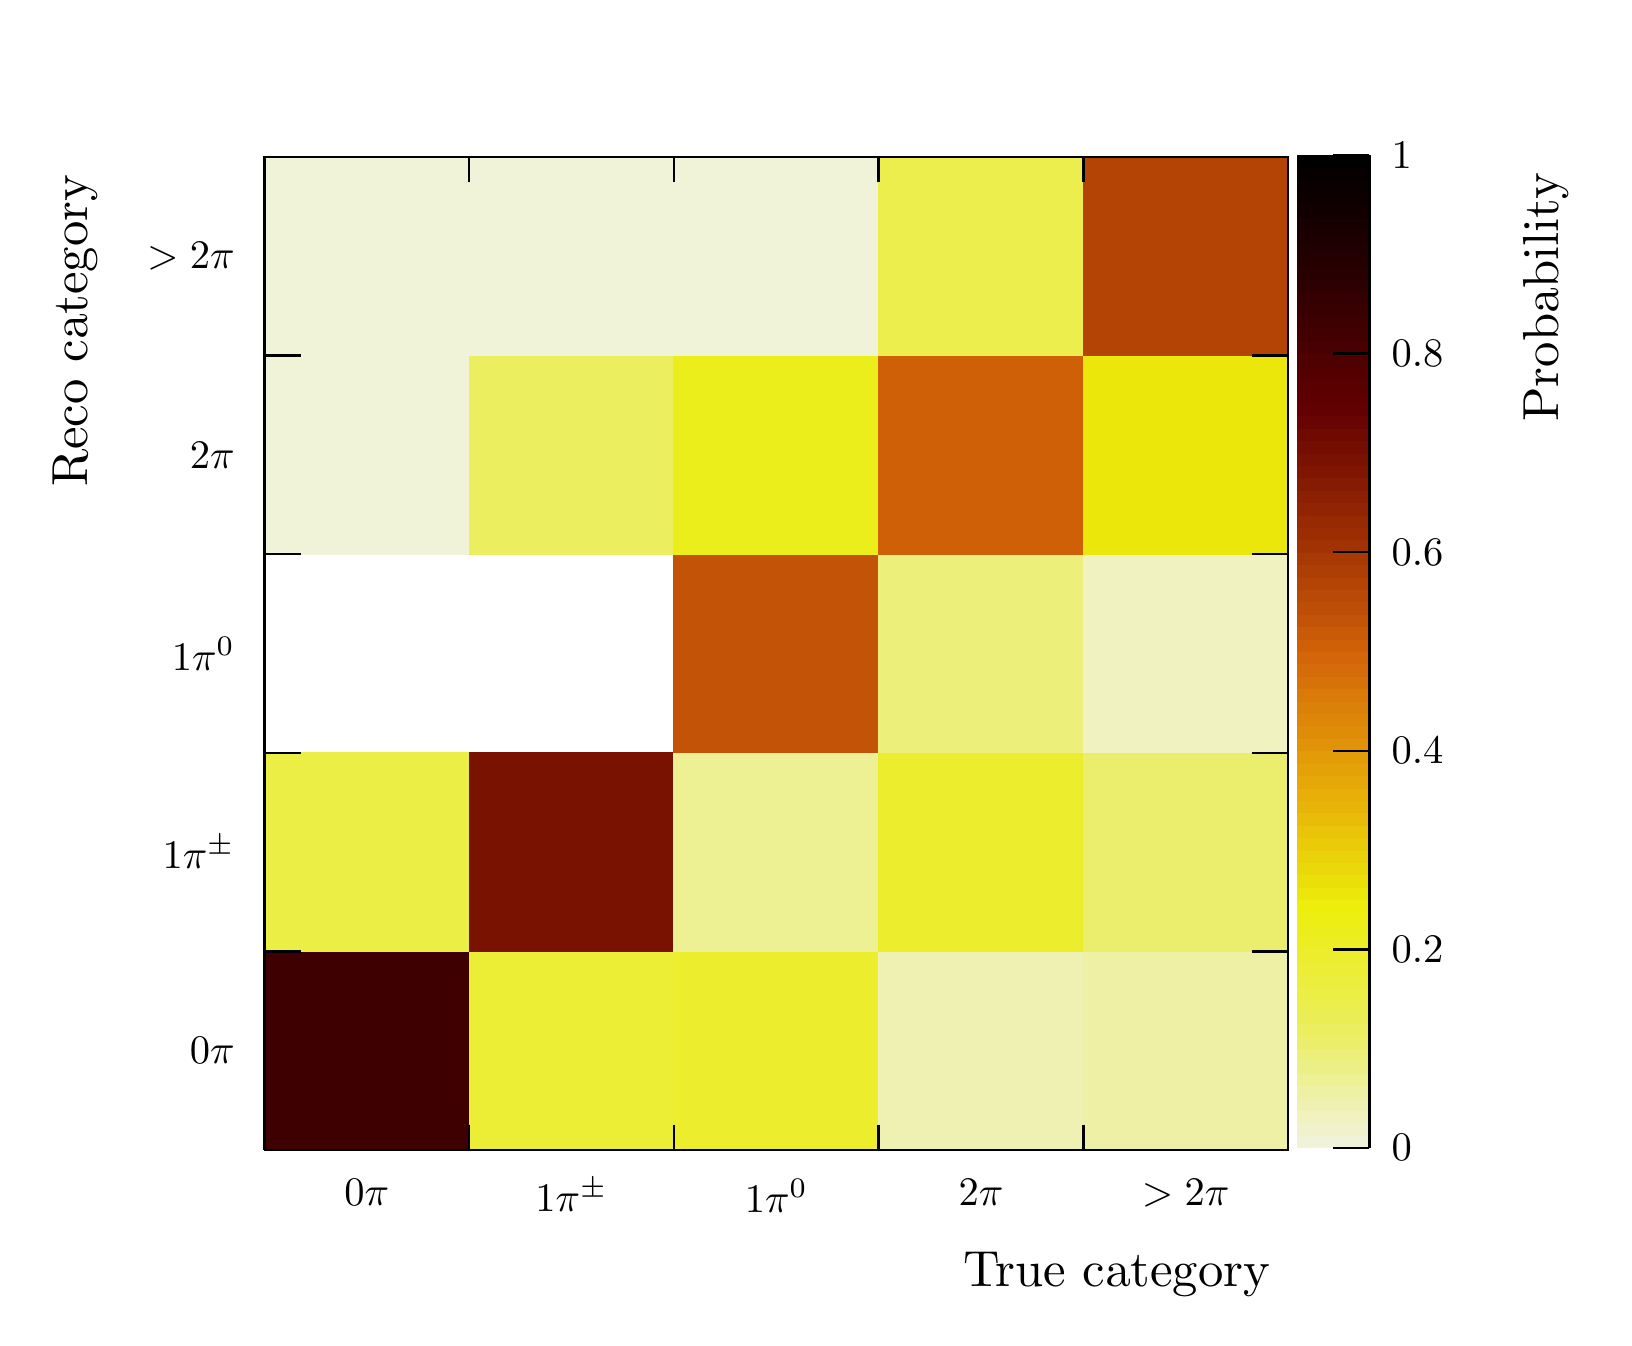
\begin{tikzpicture}
\pgfdeclareplotmark{cross} {
\pgfpathmoveto{\pgfpoint{-0.3\pgfplotmarksize}{\pgfplotmarksize}}
\pgfpathlineto{\pgfpoint{+0.3\pgfplotmarksize}{\pgfplotmarksize}}
\pgfpathlineto{\pgfpoint{+0.3\pgfplotmarksize}{0.3\pgfplotmarksize}}
\pgfpathlineto{\pgfpoint{+1\pgfplotmarksize}{0.3\pgfplotmarksize}}
\pgfpathlineto{\pgfpoint{+1\pgfplotmarksize}{-0.3\pgfplotmarksize}}
\pgfpathlineto{\pgfpoint{+0.3\pgfplotmarksize}{-0.3\pgfplotmarksize}}
\pgfpathlineto{\pgfpoint{+0.3\pgfplotmarksize}{-1.\pgfplotmarksize}}
\pgfpathlineto{\pgfpoint{-0.3\pgfplotmarksize}{-1.\pgfplotmarksize}}
\pgfpathlineto{\pgfpoint{-0.3\pgfplotmarksize}{-0.3\pgfplotmarksize}}
\pgfpathlineto{\pgfpoint{-1.\pgfplotmarksize}{-0.3\pgfplotmarksize}}
\pgfpathlineto{\pgfpoint{-1.\pgfplotmarksize}{0.3\pgfplotmarksize}}
\pgfpathlineto{\pgfpoint{-0.3\pgfplotmarksize}{0.3\pgfplotmarksize}}
\pgfpathclose
\pgfusepathqstroke
}
\pgfdeclareplotmark{cross*} {
\pgfpathmoveto{\pgfpoint{-0.3\pgfplotmarksize}{\pgfplotmarksize}}
\pgfpathlineto{\pgfpoint{+0.3\pgfplotmarksize}{\pgfplotmarksize}}
\pgfpathlineto{\pgfpoint{+0.3\pgfplotmarksize}{0.3\pgfplotmarksize}}
\pgfpathlineto{\pgfpoint{+1\pgfplotmarksize}{0.3\pgfplotmarksize}}
\pgfpathlineto{\pgfpoint{+1\pgfplotmarksize}{-0.3\pgfplotmarksize}}
\pgfpathlineto{\pgfpoint{+0.3\pgfplotmarksize}{-0.3\pgfplotmarksize}}
\pgfpathlineto{\pgfpoint{+0.3\pgfplotmarksize}{-1.\pgfplotmarksize}}
\pgfpathlineto{\pgfpoint{-0.3\pgfplotmarksize}{-1.\pgfplotmarksize}}
\pgfpathlineto{\pgfpoint{-0.3\pgfplotmarksize}{-0.3\pgfplotmarksize}}
\pgfpathlineto{\pgfpoint{-1.\pgfplotmarksize}{-0.3\pgfplotmarksize}}
\pgfpathlineto{\pgfpoint{-1.\pgfplotmarksize}{0.3\pgfplotmarksize}}
\pgfpathlineto{\pgfpoint{-0.3\pgfplotmarksize}{0.3\pgfplotmarksize}}
\pgfpathclose
\pgfusepathqfillstroke
}
\pgfdeclareplotmark{newstar} {
\pgfpathmoveto{\pgfqpoint{0pt}{\pgfplotmarksize}}
\pgfpathlineto{\pgfqpointpolar{44}{0.5\pgfplotmarksize}}
\pgfpathlineto{\pgfqpointpolar{18}{\pgfplotmarksize}}
\pgfpathlineto{\pgfqpointpolar{-20}{0.5\pgfplotmarksize}}
\pgfpathlineto{\pgfqpointpolar{-54}{\pgfplotmarksize}}
\pgfpathlineto{\pgfqpointpolar{-90}{0.5\pgfplotmarksize}}
\pgfpathlineto{\pgfqpointpolar{234}{\pgfplotmarksize}}
\pgfpathlineto{\pgfqpointpolar{198}{0.5\pgfplotmarksize}}
\pgfpathlineto{\pgfqpointpolar{162}{\pgfplotmarksize}}
\pgfpathlineto{\pgfqpointpolar{134}{0.5\pgfplotmarksize}}
\pgfpathclose
\pgfusepathqstroke
}
\pgfdeclareplotmark{newstar*} {
\pgfpathmoveto{\pgfqpoint{0pt}{\pgfplotmarksize}}
\pgfpathlineto{\pgfqpointpolar{44}{0.5\pgfplotmarksize}}
\pgfpathlineto{\pgfqpointpolar{18}{\pgfplotmarksize}}
\pgfpathlineto{\pgfqpointpolar{-20}{0.5\pgfplotmarksize}}
\pgfpathlineto{\pgfqpointpolar{-54}{\pgfplotmarksize}}
\pgfpathlineto{\pgfqpointpolar{-90}{0.5\pgfplotmarksize}}
\pgfpathlineto{\pgfqpointpolar{234}{\pgfplotmarksize}}
\pgfpathlineto{\pgfqpointpolar{198}{0.5\pgfplotmarksize}}
\pgfpathlineto{\pgfqpointpolar{162}{\pgfplotmarksize}}
\pgfpathlineto{\pgfqpointpolar{134}{0.5\pgfplotmarksize}}
\pgfpathclose
\pgfusepathqfillstroke
}
\definecolor{c}{rgb}{1,1,1};
\draw [color=c, fill=c] (0,0) rectangle (20,16.3736);
\draw [color=c, fill=c] (3,2.12857) rectangle (16,14.7363);
\definecolor{c}{rgb}{0,0,0};
\draw [c,line width=0.9] (3,2.12857) -- (3,14.7363) -- (16,14.7363) -- (16,2.12857) -- (3,2.12857);
\definecolor{c}{rgb}{1,1,1};
\draw [color=c, fill=c] (3,2.12857) rectangle (16,14.7363);
\definecolor{c}{rgb}{0,0,0};
\draw [c,line width=0.9] (3,2.12857) -- (3,14.7363) -- (16,14.7363) -- (16,2.12857) -- (3,2.12857);
\definecolor{c}{rgb}{0.242647,0,0.00392157};
\draw [color=c, fill=c] (3,2.12857) rectangle (5.6,4.65011);
\definecolor{c}{rgb}{0.923529,0.933333,0.207843};
\draw [color=c, fill=c] (5.6,2.12857) rectangle (8.2,4.65011);
\definecolor{c}{rgb}{0.924632,0.933333,0.176961};
\draw [color=c, fill=c] (8.2,2.12857) rectangle (10.8,4.65011);
\definecolor{c}{rgb}{0.936875,0.945351,0.697027};
\draw [color=c, fill=c] (10.8,2.12857) rectangle (13.4,4.65011);
\definecolor{c}{rgb}{0.933839,0.943453,0.645794};
\draw [color=c, fill=c] (13.4,2.12857) rectangle (16,4.65011);
\definecolor{c}{rgb}{0.921324,0.933333,0.269608};
\draw [color=c, fill=c] (3,4.65011) rectangle (5.6,7.17165);
\definecolor{c}{rgb}{0.479044,0.0716912,0.00710784};
\draw [color=c, fill=c] (5.6,4.65011) rectangle (8.2,7.17165);
\definecolor{c}{rgb}{0.929791,0.940923,0.577483};
\draw [color=c, fill=c] (8.2,4.65011) rectangle (10.8,7.17165);
\definecolor{c}{rgb}{0.924632,0.933333,0.176961};
\draw [color=c, fill=c] (10.8,4.65011) rectangle (13.4,7.17165);
\definecolor{c}{rgb}{0.920683,0.935231,0.423782};
\draw [color=c, fill=c] (13.4,4.65011) rectangle (16,7.17165);
\definecolor{c}{rgb}{0.762745,0.327451,0.0279412};
\draw [color=c, fill=c] (8.2,7.17165) rectangle (10.8,9.69319);
\definecolor{c}{rgb}{0.923719,0.937128,0.475016};
\draw [color=c, fill=c] (10.8,7.17165) rectangle (13.4,9.69319);
\definecolor{c}{rgb}{0.939911,0.947249,0.748261};
\draw [color=c, fill=c] (13.4,7.17165) rectangle (16,9.69319);
\definecolor{c}{rgb}{0.945984,0.951044,0.850727};
\draw [color=c, fill=c] (3,9.69319) rectangle (5.6,12.2147);
\definecolor{c}{rgb}{0.917647,0.933333,0.372549};
\draw [color=c, fill=c] (5.6,9.69319) rectangle (8.2,12.2147);
\definecolor{c}{rgb}{0.927206,0.933333,0.104902};
\draw [color=c, fill=c] (8.2,9.69319) rectangle (10.8,12.2147);
\definecolor{c}{rgb}{0.810784,0.37549,0.0330882};
\draw [color=c, fill=c] (10.8,9.69319) rectangle (13.4,12.2147);
\definecolor{c}{rgb}{0.926838,0.907598,0.0420343};
\draw [color=c, fill=c] (13.4,9.69319) rectangle (16,12.2147);
\definecolor{c}{rgb}{0.945984,0.951044,0.850727};
\draw [color=c, fill=c] (3,12.2147) rectangle (5.6,14.7363);
\draw [color=c, fill=c] (5.6,12.2147) rectangle (8.2,14.7363);
\draw [color=c, fill=c] (8.2,12.2147) rectangle (10.8,14.7363);
\definecolor{c}{rgb}{0.920221,0.933333,0.30049};
\draw [color=c, fill=c] (10.8,12.2147) rectangle (13.4,14.7363);
\definecolor{c}{rgb}{0.70098,0.265686,0.0213235};
\draw [color=c, fill=c] (13.4,12.2147) rectangle (16,14.7363);
\definecolor{c}{rgb}{0,0,0};
\draw [c,line width=0.9] (3,2.12857) -- (16,2.12857);
\draw [anchor=north] (4.3,1.93946) node[scale=1.46438, color=c, rotate=0]{$0\pi$};
\draw [anchor=north] (6.9,1.93946) node[scale=1.46438, color=c, rotate=0]{$1\pi^{\pm}$};
\draw [anchor=north] (9.5,1.93946) node[scale=1.46438, color=c, rotate=0]{$1\pi^{0}$};
\draw [anchor=north] (12.1,1.93946) node[scale=1.46438, color=c, rotate=0]{$2\pi$};
\draw [anchor=north] (14.7,1.93946) node[scale=1.46438, color=c, rotate=0]{$>2\pi$};
\draw [c,line width=0.9] (3,2.44786) -- (3,2.12857);
\draw [c,line width=0.9] (5.6,2.44786) -- (5.6,2.12857);
\draw [c,line width=0.9] (8.2,2.44786) -- (8.2,2.12857);
\draw [c,line width=0.9] (10.8,2.44786) -- (10.8,2.12857);
\draw [c,line width=0.9] (13.4,2.44786) -- (13.4,2.12857);
\draw [c,line width=0.9] (16,2.44786) -- (16,2.12857);
\draw [anchor= east] (16,0.556703) node[scale=1.83047, color=c, rotate=0]{True category};
\draw [c,line width=0.9] (3,14.7363) -- (16,14.7363);
\draw [c,line width=0.9] (3,14.417) -- (3,14.7363);
\draw [c,line width=0.9] (5.6,14.417) -- (5.6,14.7363);
\draw [c,line width=0.9] (8.2,14.417) -- (8.2,14.7363);
\draw [c,line width=0.9] (10.8,14.417) -- (10.8,14.7363);
\draw [c,line width=0.9] (13.4,14.417) -- (13.4,14.7363);
\draw [c,line width=0.9] (16,14.417) -- (16,14.7363);
\draw [c,line width=0.9] (3,2.12857) -- (3,14.7363);
\draw [anchor= east] (2.805,3.38934) node[scale=1.46438, color=c, rotate=0]{$0\pi$};
\draw [anchor= east] (2.805,5.91088) node[scale=1.46438, color=c, rotate=0]{$1\pi^{\pm}$};
\draw [anchor= east] (2.805,8.43242) node[scale=1.46438, color=c, rotate=0]{$1\pi^{0}$};
\draw [anchor= east] (2.805,10.954) node[scale=1.46438, color=c, rotate=0]{$2\pi$};
\draw [anchor= east] (2.805,13.4755) node[scale=1.46438, color=c, rotate=0]{$>2\pi$};
\draw [c,line width=0.9] (3.462,2.12857) -- (3,2.12857);
\draw [c,line width=0.9] (3.462,4.65011) -- (3,4.65011);
\draw [c,line width=0.9] (3.462,7.17165) -- (3,7.17165);
\draw [c,line width=0.9] (3.462,9.69319) -- (3,9.69319);
\draw [c,line width=0.9] (3.462,12.2147) -- (3,12.2147);
\draw [c,line width=0.9] (3.462,14.7363) -- (3,14.7363);
\draw [anchor= east] (0.6,14.7363) node[scale=1.83047, color=c, rotate=90]{Reco category};
\draw [c,line width=0.9] (16,2.12857) -- (16,14.7363);
\draw [c,line width=0.9] (15.538,2.12857) -- (16,2.12857);
\draw [c,line width=0.9] (15.538,4.65011) -- (16,4.65011);
\draw [c,line width=0.9] (15.538,7.17165) -- (16,7.17165);
\draw [c,line width=0.9] (15.538,9.69319) -- (16,9.69319);
\draw [c,line width=0.9] (15.538,12.2147) -- (16,12.2147);
\draw [c,line width=0.9] (15.538,14.7363) -- (16,14.7363);
\definecolor{c}{rgb}{0.945984,0.951044,0.850727};
\draw [color=c, fill=c] (16.1264,2.15514) rectangle (17.033,2.31271);
\definecolor{c}{rgb}{0.942948,0.949146,0.799494};
\draw [color=c, fill=c] (16.1264,2.31271) rectangle (17.033,2.47028);
\definecolor{c}{rgb}{0.939911,0.947249,0.748261};
\draw [color=c, fill=c] (16.1264,2.47028) rectangle (17.033,2.62785);
\definecolor{c}{rgb}{0.936875,0.945351,0.697027};
\draw [color=c, fill=c] (16.1264,2.62785) rectangle (17.033,2.78541);
\definecolor{c}{rgb}{0.933839,0.943453,0.645794};
\draw [color=c, fill=c] (16.1264,2.78541) rectangle (17.033,2.94298);
\definecolor{c}{rgb}{0.929791,0.940923,0.577483};
\draw [color=c, fill=c] (16.1264,2.94298) rectangle (17.033,3.10055);
\definecolor{c}{rgb}{0.926755,0.939026,0.526249};
\draw [color=c, fill=c] (16.1264,3.10055) rectangle (17.033,3.25812);
\definecolor{c}{rgb}{0.923719,0.937128,0.475016};
\draw [color=c, fill=c] (16.1264,3.25812) rectangle (17.033,3.41569);
\definecolor{c}{rgb}{0.920683,0.935231,0.423782};
\draw [color=c, fill=c] (16.1264,3.41569) rectangle (17.033,3.57326);
\definecolor{c}{rgb}{0.917647,0.933333,0.372549};
\draw [color=c, fill=c] (16.1264,3.57326) rectangle (17.033,3.73083);
\definecolor{c}{rgb}{0.919118,0.933333,0.331373};
\draw [color=c, fill=c] (16.1264,3.73083) rectangle (17.033,3.8884);
\definecolor{c}{rgb}{0.920221,0.933333,0.30049};
\draw [color=c, fill=c] (16.1264,3.8884) rectangle (17.033,4.04597);
\definecolor{c}{rgb}{0.921324,0.933333,0.269608};
\draw [color=c, fill=c] (16.1264,4.04597) rectangle (17.033,4.20354);
\definecolor{c}{rgb}{0.922426,0.933333,0.238725};
\draw [color=c, fill=c] (16.1264,4.20354) rectangle (17.033,4.3611);
\definecolor{c}{rgb}{0.923529,0.933333,0.207843};
\draw [color=c, fill=c] (16.1264,4.3611) rectangle (17.033,4.51867);
\definecolor{c}{rgb}{0.924632,0.933333,0.176961};
\draw [color=c, fill=c] (16.1264,4.51867) rectangle (17.033,4.67624);
\definecolor{c}{rgb}{0.926103,0.933333,0.135784};
\draw [color=c, fill=c] (16.1264,4.67624) rectangle (17.033,4.83381);
\definecolor{c}{rgb}{0.927206,0.933333,0.104902};
\draw [color=c, fill=c] (16.1264,4.83381) rectangle (17.033,4.99138);
\definecolor{c}{rgb}{0.928309,0.933333,0.0740196};
\draw [color=c, fill=c] (16.1264,4.99138) rectangle (17.033,5.14895);
\definecolor{c}{rgb}{0.929412,0.933333,0.0431373};
\draw [color=c, fill=c] (16.1264,5.14895) rectangle (17.033,5.30652);
\definecolor{c}{rgb}{0.926838,0.907598,0.0420343};
\draw [color=c, fill=c] (16.1264,5.30652) rectangle (17.033,5.46409);
\definecolor{c}{rgb}{0.923407,0.873284,0.0405637};
\draw [color=c, fill=c] (16.1264,5.46409) rectangle (17.033,5.62166);
\definecolor{c}{rgb}{0.920833,0.847549,0.0394608};
\draw [color=c, fill=c] (16.1264,5.62166) rectangle (17.033,5.77923);
\definecolor{c}{rgb}{0.91826,0.821814,0.0383578};
\draw [color=c, fill=c] (16.1264,5.77923) rectangle (17.033,5.9368);
\definecolor{c}{rgb}{0.915686,0.796078,0.0372549};
\draw [color=c, fill=c] (16.1264,5.9368) rectangle (17.033,6.09436);
\definecolor{c}{rgb}{0.913113,0.770343,0.036152};
\draw [color=c, fill=c] (16.1264,6.09436) rectangle (17.033,6.25193);
\definecolor{c}{rgb}{0.909681,0.736029,0.0346814};
\draw [color=c, fill=c] (16.1264,6.25193) rectangle (17.033,6.4095);
\definecolor{c}{rgb}{0.907108,0.710294,0.0335784};
\draw [color=c, fill=c] (16.1264,6.4095) rectangle (17.033,6.56707);
\definecolor{c}{rgb}{0.904534,0.684559,0.0324755};
\draw [color=c, fill=c] (16.1264,6.56707) rectangle (17.033,6.72464);
\definecolor{c}{rgb}{0.901961,0.658824,0.0313726};
\draw [color=c, fill=c] (16.1264,6.72464) rectangle (17.033,6.88221);
\definecolor{c}{rgb}{0.895343,0.634191,0.0317402};
\draw [color=c, fill=c] (16.1264,6.88221) rectangle (17.033,7.03978);
\definecolor{c}{rgb}{0.888726,0.609559,0.0321078};
\draw [color=c, fill=c] (16.1264,7.03978) rectangle (17.033,7.19735);
\definecolor{c}{rgb}{0.879902,0.576716,0.032598};
\draw [color=c, fill=c] (16.1264,7.19735) rectangle (17.033,7.35492);
\definecolor{c}{rgb}{0.873284,0.552083,0.0329657};
\draw [color=c, fill=c] (16.1264,7.35492) rectangle (17.033,7.51249);
\definecolor{c}{rgb}{0.866667,0.527451,0.0333333};
\draw [color=c, fill=c] (16.1264,7.51249) rectangle (17.033,7.67005);
\definecolor{c}{rgb}{0.860049,0.502819,0.033701};
\draw [color=c, fill=c] (16.1264,7.67005) rectangle (17.033,7.82762);
\definecolor{c}{rgb}{0.853431,0.478186,0.0340686};
\draw [color=c, fill=c] (16.1264,7.82762) rectangle (17.033,7.98519);
\definecolor{c}{rgb}{0.844608,0.445343,0.0345588};
\draw [color=c, fill=c] (16.1264,7.98519) rectangle (17.033,8.14276);
\definecolor{c}{rgb}{0.83799,0.420711,0.0349265};
\draw [color=c, fill=c] (16.1264,8.14276) rectangle (17.033,8.30033);
\definecolor{c}{rgb}{0.831373,0.396078,0.0352941};
\draw [color=c, fill=c] (16.1264,8.30033) rectangle (17.033,8.4579);
\definecolor{c}{rgb}{0.810784,0.37549,0.0330882};
\draw [color=c, fill=c] (16.1264,8.4579) rectangle (17.033,8.61547);
\definecolor{c}{rgb}{0.790196,0.354902,0.0308824};
\draw [color=c, fill=c] (16.1264,8.61547) rectangle (17.033,8.77304);
\definecolor{c}{rgb}{0.762745,0.327451,0.0279412};
\draw [color=c, fill=c] (16.1264,8.77304) rectangle (17.033,8.93061);
\definecolor{c}{rgb}{0.742157,0.306863,0.0257353};
\draw [color=c, fill=c] (16.1264,8.93061) rectangle (17.033,9.08818);
\definecolor{c}{rgb}{0.721569,0.286275,0.0235294};
\draw [color=c, fill=c] (16.1264,9.08818) rectangle (17.033,9.24574);
\definecolor{c}{rgb}{0.70098,0.265686,0.0213235};
\draw [color=c, fill=c] (16.1264,9.24574) rectangle (17.033,9.40331);
\definecolor{c}{rgb}{0.680392,0.245098,0.0191176};
\draw [color=c, fill=c] (16.1264,9.40331) rectangle (17.033,9.56088);
\definecolor{c}{rgb}{0.659804,0.22451,0.0169118};
\draw [color=c, fill=c] (16.1264,9.56088) rectangle (17.033,9.71845);
\definecolor{c}{rgb}{0.632353,0.197059,0.0139706};
\draw [color=c, fill=c] (16.1264,9.71845) rectangle (17.033,9.87602);
\definecolor{c}{rgb}{0.611765,0.176471,0.0117647};
\draw [color=c, fill=c] (16.1264,9.87602) rectangle (17.033,10.0336);
\definecolor{c}{rgb}{0.590809,0.159926,0.0110294};
\draw [color=c, fill=c] (16.1264,10.0336) rectangle (17.033,10.1912);
\definecolor{c}{rgb}{0.569853,0.143382,0.0102941};
\draw [color=c, fill=c] (16.1264,10.1912) rectangle (17.033,10.3487);
\definecolor{c}{rgb}{0.548897,0.126838,0.00955882};
\draw [color=c, fill=c] (16.1264,10.3487) rectangle (17.033,10.5063);
\definecolor{c}{rgb}{0.520956,0.104779,0.00857843};
\draw [color=c, fill=c] (16.1264,10.5063) rectangle (17.033,10.6639);
\definecolor{c}{rgb}{0.5,0.0882353,0.00784314};
\draw [color=c, fill=c] (16.1264,10.6639) rectangle (17.033,10.8214);
\definecolor{c}{rgb}{0.479044,0.0716912,0.00710784};
\draw [color=c, fill=c] (16.1264,10.8214) rectangle (17.033,10.979);
\definecolor{c}{rgb}{0.458088,0.0551471,0.00637255};
\draw [color=c, fill=c] (16.1264,10.979) rectangle (17.033,11.1366);
\definecolor{c}{rgb}{0.437132,0.0386029,0.00563726};
\draw [color=c, fill=c] (16.1264,11.1366) rectangle (17.033,11.2941);
\definecolor{c}{rgb}{0.409191,0.0165441,0.00465686};
\draw [color=c, fill=c] (16.1264,11.2941) rectangle (17.033,11.4517);
\definecolor{c}{rgb}{0.388235,0,0.00392157};
\draw [color=c, fill=c] (16.1264,11.4517) rectangle (17.033,11.6093);
\definecolor{c}{rgb}{0.368382,0,0.00392157};
\draw [color=c, fill=c] (16.1264,11.6093) rectangle (17.033,11.7668);
\definecolor{c}{rgb}{0.348529,0,0.00392157};
\draw [color=c, fill=c] (16.1264,11.7668) rectangle (17.033,11.9244);
\definecolor{c}{rgb}{0.328676,0,0.00392157};
\draw [color=c, fill=c] (16.1264,11.9244) rectangle (17.033,12.082);
\definecolor{c}{rgb}{0.308824,0,0.00392157};
\draw [color=c, fill=c] (16.1264,12.082) rectangle (17.033,12.2396);
\definecolor{c}{rgb}{0.282353,0,0.00392157};
\draw [color=c, fill=c] (16.1264,12.2396) rectangle (17.033,12.3971);
\definecolor{c}{rgb}{0.2625,0,0.00392157};
\draw [color=c, fill=c] (16.1264,12.3971) rectangle (17.033,12.5547);
\definecolor{c}{rgb}{0.242647,0,0.00392157};
\draw [color=c, fill=c] (16.1264,12.5547) rectangle (17.033,12.7123);
\definecolor{c}{rgb}{0.222794,0,0.00392157};
\draw [color=c, fill=c] (16.1264,12.7123) rectangle (17.033,12.8698);
\definecolor{c}{rgb}{0.202941,0,0.00392157};
\draw [color=c, fill=c] (16.1264,12.8698) rectangle (17.033,13.0274);
\definecolor{c}{rgb}{0.176471,0,0.00392157};
\draw [color=c, fill=c] (16.1264,13.0274) rectangle (17.033,13.185);
\definecolor{c}{rgb}{0.159926,0,0.00355392};
\draw [color=c, fill=c] (16.1264,13.185) rectangle (17.033,13.3425);
\definecolor{c}{rgb}{0.143382,0,0.00318627};
\draw [color=c, fill=c] (16.1264,13.3425) rectangle (17.033,13.5001);
\definecolor{c}{rgb}{0.126838,0,0.00281863};
\draw [color=c, fill=c] (16.1264,13.5001) rectangle (17.033,13.6577);
\definecolor{c}{rgb}{0.110294,0,0.00245098};
\draw [color=c, fill=c] (16.1264,13.6577) rectangle (17.033,13.8152);
\definecolor{c}{rgb}{0.0882353,0,0.00196078};
\draw [color=c, fill=c] (16.1264,13.8152) rectangle (17.033,13.9728);
\definecolor{c}{rgb}{0.0716912,0,0.00159314};
\draw [color=c, fill=c] (16.1264,13.9728) rectangle (17.033,14.1304);
\definecolor{c}{rgb}{0.0551471,0,0.00122549};
\draw [color=c, fill=c] (16.1264,14.1304) rectangle (17.033,14.288);
\definecolor{c}{rgb}{0.0386029,0,0.000857843};
\draw [color=c, fill=c] (16.1264,14.288) rectangle (17.033,14.4455);
\definecolor{c}{rgb}{0.0220588,0,0.000490196};
\draw [color=c, fill=c] (16.1264,14.4455) rectangle (17.033,14.6031);
\definecolor{c}{rgb}{0.00551471,0,0.000122549};
\draw [color=c, fill=c] (16.1264,14.6031) rectangle (17.033,14.7607);
\definecolor{c}{rgb}{0,0,0};
\draw [c,line width=0.9] (17.033,2.15514) -- (17.033,14.7607);
\draw [c,line width=0.9] (16.571,2.15514) -- (17.033,2.15514);
\draw [c,line width=0.9] (16.571,4.67624) -- (17.033,4.67624);
\draw [c,line width=0.9] (16.571,7.19735) -- (17.033,7.19735);
\draw [c,line width=0.9] (16.571,9.71845) -- (17.033,9.71845);
\draw [c,line width=0.9] (16.571,12.2396) -- (17.033,12.2396);
\draw [c,line width=0.9] (16.571,14.7607) -- (17.033,14.7607);
\draw [c,line width=0.9] (16.571,14.7607) -- (17.033,14.7607);
\draw [anchor= west] (17.133,2.15514) node[scale=1.46438, color=c, rotate=0]{0};
\draw [anchor= west] (17.133,4.67624) node[scale=1.46438, color=c, rotate=0]{0.2};
\draw [anchor= west] (17.133,7.19735) node[scale=1.46438, color=c, rotate=0]{0.4};
\draw [anchor= west] (17.133,9.71845) node[scale=1.46438, color=c, rotate=0]{0.6};
\draw [anchor= west] (17.133,12.2396) node[scale=1.46438, color=c, rotate=0]{0.8};
\draw [anchor= west] (17.133,14.7607) node[scale=1.46438, color=c, rotate=0]{1};
\draw [anchor= east] (19.273,14.7607) node[scale=1.83047, color=c, rotate=90]{Probability};
\end{tikzpicture}

	\end{adjustbox}
	\caption[Final state pion multiplicity confusion matrix from ND-LAr simulations]{Final state pion multiplicity confusion matrix from ND-LAr simulations, from~\cite{ndCdr}. The colour axis is probability.}
	\label{fig:larConfusMat}
\end{figure}

\citefig{fig:q2LarFhc} shows the ND-LAr equivalent to \citefigL{fig:Q2CompFhc}. 
Here, one can see that the errors are larger in most cases (compared to \citefigL{fig:Q2CompFhc}) due to the increased confusion between categories.
However, in spite of this, it still seems that significant differences are visible for some of the final state topologies in ND-LAr.

\begin{figure}[h]
	\centering
	\includegraphics[width=.6\linewidth]{files/figures/dune_ndrwt/larQ2Reco}
	\caption[Ratio of $Q^{2}_{\textrm{reco}}$ between GENIE and NuWro mock data in ND-LAr]{Ratio of $Q^{2}_{\textrm{reco}}$ between GENIE and NuWro mock data in ND-LAr, from~\cite{ndCdr}. Bins with $<100$ MC events are suppressed.}
	\label{fig:q2LarFhc}	
\end{figure}

\section{Near detector-driven reweighting}
\label{sec:dune_ndrwt:rwt}

% Why we have a near detector
As mentioned in \citesec{sec:dune:nd}, one of the reasons for the inclusion of a near detector in a long baseline neutrino oscillation experiment to allow the constraint of various neutrino cross-section systematics.
However, it may be that existing neutrino interaction models and their associated uncertainties do not explain the observed reconstructed neutrino energy spectra.

%% If we observe some cross-section effect that is not explained by our model in ND what do we do?

\citefig{fig:fdSamplesPostFit} shows the four far detector samples (one appearance and one disappearance for each horn current) used in a typical oscillation analysis.
For each sample the nominal GENIE MC is plotted in blue along with the NuWro `mock data' as black points.

The red line shows the post-fit result of a far detector-only fit with all flux, detector and cross-section systematics at their nominal values. 
For the purposes of this fit the nominal MC is GENIE and the data is the NuWro `mock data'.
The $\chi^{2}$ value for the post-fit distribution is 2.29 indicating good agreement.

\begin{figure}[h]
	\begin{subfigure}[t]{0.5\linewidth}
		\begin{adjustbox}{max totalsize=\linewidth, center}
			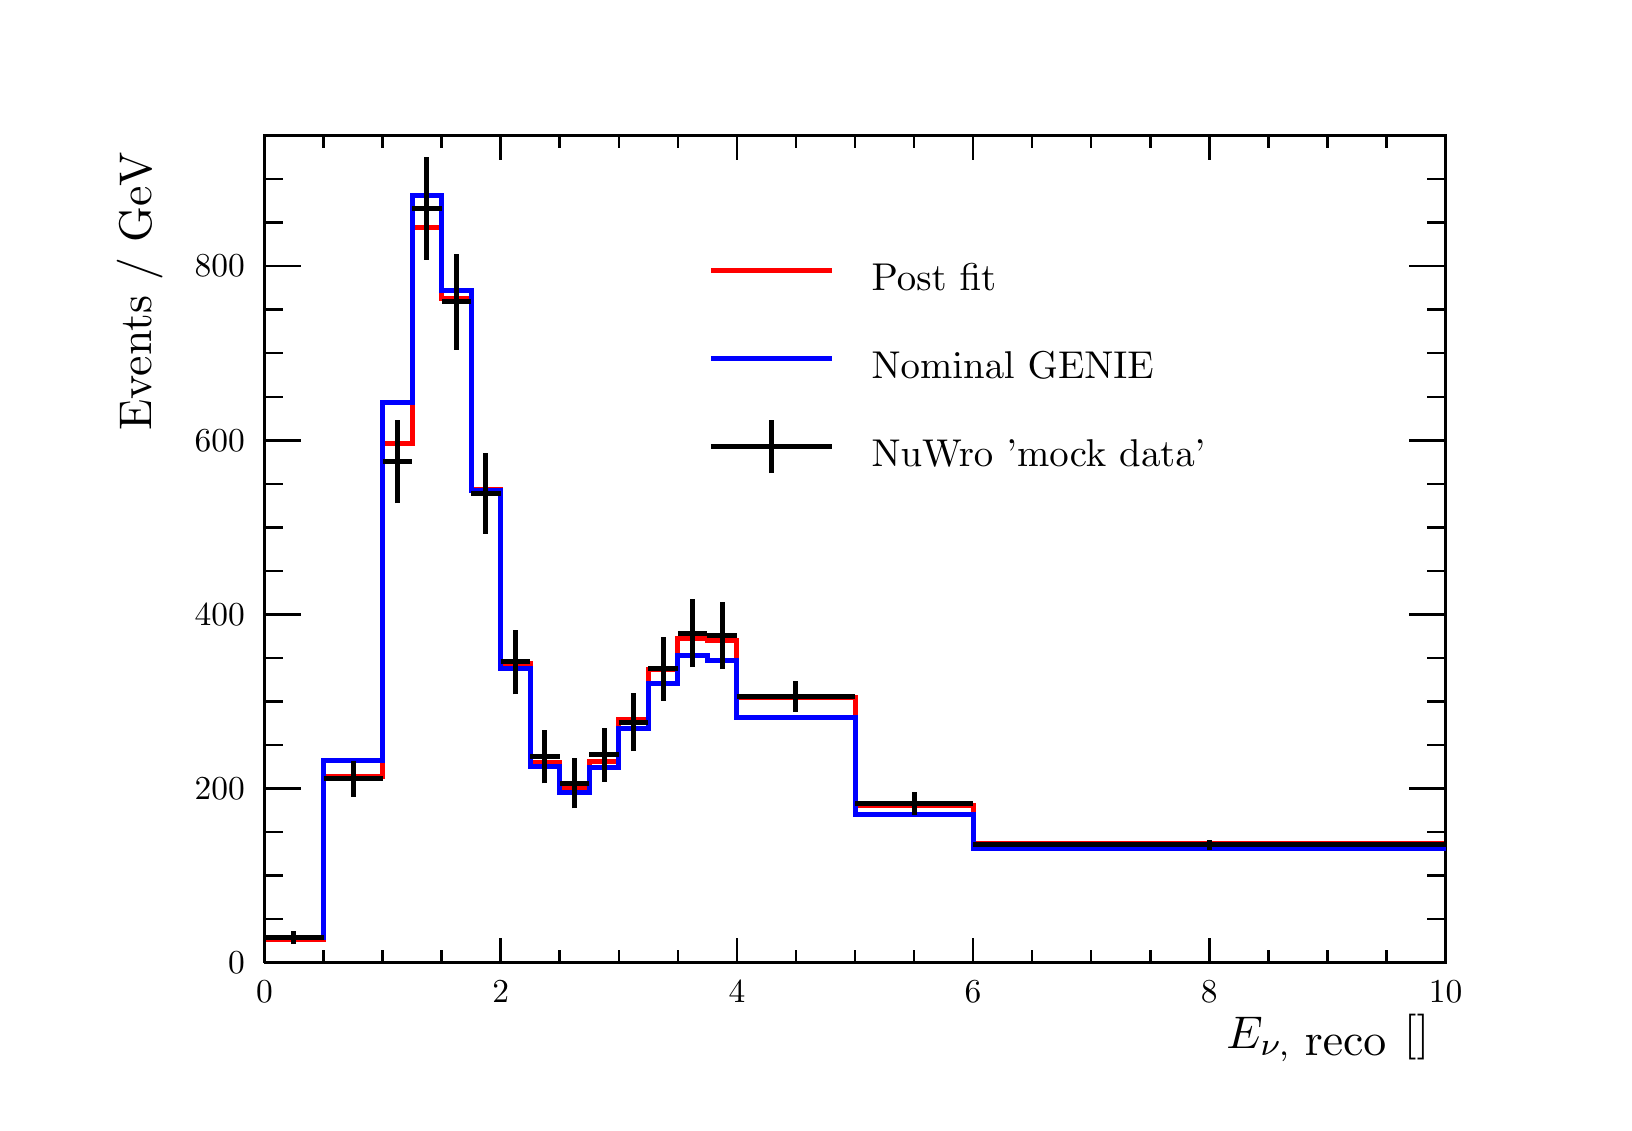
\begin{tikzpicture}
\pgfdeclareplotmark{cross} {
\pgfpathmoveto{\pgfpoint{-0.3\pgfplotmarksize}{\pgfplotmarksize}}
\pgfpathlineto{\pgfpoint{+0.3\pgfplotmarksize}{\pgfplotmarksize}}
\pgfpathlineto{\pgfpoint{+0.3\pgfplotmarksize}{0.3\pgfplotmarksize}}
\pgfpathlineto{\pgfpoint{+1\pgfplotmarksize}{0.3\pgfplotmarksize}}
\pgfpathlineto{\pgfpoint{+1\pgfplotmarksize}{-0.3\pgfplotmarksize}}
\pgfpathlineto{\pgfpoint{+0.3\pgfplotmarksize}{-0.3\pgfplotmarksize}}
\pgfpathlineto{\pgfpoint{+0.3\pgfplotmarksize}{-1.\pgfplotmarksize}}
\pgfpathlineto{\pgfpoint{-0.3\pgfplotmarksize}{-1.\pgfplotmarksize}}
\pgfpathlineto{\pgfpoint{-0.3\pgfplotmarksize}{-0.3\pgfplotmarksize}}
\pgfpathlineto{\pgfpoint{-1.\pgfplotmarksize}{-0.3\pgfplotmarksize}}
\pgfpathlineto{\pgfpoint{-1.\pgfplotmarksize}{0.3\pgfplotmarksize}}
\pgfpathlineto{\pgfpoint{-0.3\pgfplotmarksize}{0.3\pgfplotmarksize}}
\pgfpathclose
\pgfusepathqstroke
}
\pgfdeclareplotmark{cross*} {
\pgfpathmoveto{\pgfpoint{-0.3\pgfplotmarksize}{\pgfplotmarksize}}
\pgfpathlineto{\pgfpoint{+0.3\pgfplotmarksize}{\pgfplotmarksize}}
\pgfpathlineto{\pgfpoint{+0.3\pgfplotmarksize}{0.3\pgfplotmarksize}}
\pgfpathlineto{\pgfpoint{+1\pgfplotmarksize}{0.3\pgfplotmarksize}}
\pgfpathlineto{\pgfpoint{+1\pgfplotmarksize}{-0.3\pgfplotmarksize}}
\pgfpathlineto{\pgfpoint{+0.3\pgfplotmarksize}{-0.3\pgfplotmarksize}}
\pgfpathlineto{\pgfpoint{+0.3\pgfplotmarksize}{-1.\pgfplotmarksize}}
\pgfpathlineto{\pgfpoint{-0.3\pgfplotmarksize}{-1.\pgfplotmarksize}}
\pgfpathlineto{\pgfpoint{-0.3\pgfplotmarksize}{-0.3\pgfplotmarksize}}
\pgfpathlineto{\pgfpoint{-1.\pgfplotmarksize}{-0.3\pgfplotmarksize}}
\pgfpathlineto{\pgfpoint{-1.\pgfplotmarksize}{0.3\pgfplotmarksize}}
\pgfpathlineto{\pgfpoint{-0.3\pgfplotmarksize}{0.3\pgfplotmarksize}}
\pgfpathclose
\pgfusepathqfillstroke
}
\pgfdeclareplotmark{newstar} {
\pgfpathmoveto{\pgfqpoint{0pt}{\pgfplotmarksize}}
\pgfpathlineto{\pgfqpointpolar{44}{0.5\pgfplotmarksize}}
\pgfpathlineto{\pgfqpointpolar{18}{\pgfplotmarksize}}
\pgfpathlineto{\pgfqpointpolar{-20}{0.5\pgfplotmarksize}}
\pgfpathlineto{\pgfqpointpolar{-54}{\pgfplotmarksize}}
\pgfpathlineto{\pgfqpointpolar{-90}{0.5\pgfplotmarksize}}
\pgfpathlineto{\pgfqpointpolar{234}{\pgfplotmarksize}}
\pgfpathlineto{\pgfqpointpolar{198}{0.5\pgfplotmarksize}}
\pgfpathlineto{\pgfqpointpolar{162}{\pgfplotmarksize}}
\pgfpathlineto{\pgfqpointpolar{134}{0.5\pgfplotmarksize}}
\pgfpathclose
\pgfusepathqstroke
}
\pgfdeclareplotmark{newstar*} {
\pgfpathmoveto{\pgfqpoint{0pt}{\pgfplotmarksize}}
\pgfpathlineto{\pgfqpointpolar{44}{0.5\pgfplotmarksize}}
\pgfpathlineto{\pgfqpointpolar{18}{\pgfplotmarksize}}
\pgfpathlineto{\pgfqpointpolar{-20}{0.5\pgfplotmarksize}}
\pgfpathlineto{\pgfqpointpolar{-54}{\pgfplotmarksize}}
\pgfpathlineto{\pgfqpointpolar{-90}{0.5\pgfplotmarksize}}
\pgfpathlineto{\pgfqpointpolar{234}{\pgfplotmarksize}}
\pgfpathlineto{\pgfqpointpolar{198}{0.5\pgfplotmarksize}}
\pgfpathlineto{\pgfqpointpolar{162}{\pgfplotmarksize}}
\pgfpathlineto{\pgfqpointpolar{134}{0.5\pgfplotmarksize}}
\pgfpathclose
\pgfusepathqfillstroke
}
\definecolor{c}{rgb}{1,1,1};
\draw [color=c, fill=c] (0,0) rectangle (20,13.639);
\draw [color=c, fill=c] (3,1.77307) rectangle (18,12.2751);
\definecolor{c}{rgb}{0,0,0};
\draw [c,line width=0.9] (3,1.77307) -- (3,12.2751) -- (18,12.2751) -- (18,1.77307) -- (3,1.77307);
\definecolor{c}{rgb}{1,1,1};
\draw [color=c, fill=c] (3,1.77307) rectangle (18,12.2751);
\definecolor{c}{rgb}{0,0,0};
\draw [c,line width=0.9] (3,1.77307) -- (3,12.2751) -- (18,12.2751) -- (18,1.77307) -- (3,1.77307);
\definecolor{c}{rgb}{1,0,0};
\draw [c,line width=1.8] (3,2.07023) -- (3.75,2.07023) -- (3.75,4.13781) -- (4.5,4.13781) -- (4.5,8.35958) -- (4.875,8.35958) -- (4.875,11.111) -- (5.25,11.111) -- (5.25,10.2102) -- (5.625,10.2102) -- (5.625,7.78333) -- (6,7.78333) -- (6,5.56806) --
 (6.375,5.56806) -- (6.375,4.31399) -- (6.75,4.31399) -- (6.75,3.99747) -- (7.125,3.99747) -- (7.125,4.32564) -- (7.5,4.32564) -- (7.5,4.85745) -- (7.875,4.85745) -- (7.875,5.49486) -- (8.25,5.49486) -- (8.25,5.88922) -- (8.625,5.88922) --
 (8.625,5.8639) -- (9,5.8639) -- (9,5.14297) -- (10.5,5.14297) -- (10.5,3.77082) -- (12,3.77082) -- (12,3.28705) -- (18,3.28705);
\definecolor{c}{rgb}{0,0,0};
\draw [c,line width=0.9] (3,1.77307) -- (18,1.77307);
\draw [c,line width=0.9] (3,2.07994) -- (3,1.77307);
\draw [c,line width=0.9] (3.75,1.9265) -- (3.75,1.77307);
\draw [c,line width=0.9] (4.5,1.9265) -- (4.5,1.77307);
\draw [c,line width=0.9] (5.25,1.9265) -- (5.25,1.77307);
\draw [c,line width=0.9] (6,2.07994) -- (6,1.77307);
\draw [c,line width=0.9] (6.75,1.9265) -- (6.75,1.77307);
\draw [c,line width=0.9] (7.5,1.9265) -- (7.5,1.77307);
\draw [c,line width=0.9] (8.25,1.9265) -- (8.25,1.77307);
\draw [c,line width=0.9] (9,2.07994) -- (9,1.77307);
\draw [c,line width=0.9] (9.75,1.9265) -- (9.75,1.77307);
\draw [c,line width=0.9] (10.5,1.9265) -- (10.5,1.77307);
\draw [c,line width=0.9] (11.25,1.9265) -- (11.25,1.77307);
\draw [c,line width=0.9] (12,2.07994) -- (12,1.77307);
\draw [c,line width=0.9] (12.75,1.9265) -- (12.75,1.77307);
\draw [c,line width=0.9] (13.5,1.9265) -- (13.5,1.77307);
\draw [c,line width=0.9] (14.25,1.9265) -- (14.25,1.77307);
\draw [c,line width=0.9] (15,2.07994) -- (15,1.77307);
\draw [c,line width=0.9] (15.75,1.9265) -- (15.75,1.77307);
\draw [c,line width=0.9] (16.5,1.9265) -- (16.5,1.77307);
\draw [c,line width=0.9] (17.25,1.9265) -- (17.25,1.77307);
\draw [c,line width=0.9] (18,2.07994) -- (18,1.77307);
\draw [anchor=base] (3,1.26842) node[scale=1.20912, color=c, rotate=0]{0};
\draw [anchor=base] (6,1.26842) node[scale=1.20912, color=c, rotate=0]{2};
\draw [anchor=base] (9,1.26842) node[scale=1.20912, color=c, rotate=0]{4};
\draw [anchor=base] (12,1.26842) node[scale=1.20912, color=c, rotate=0]{6};
\draw [anchor=base] (15,1.26842) node[scale=1.20912, color=c, rotate=0]{8};
\draw [anchor=base] (18,1.26842) node[scale=1.20912, color=c, rotate=0]{10};
\draw [anchor= east] (18,0.812882) node[scale=1.65459, color=c, rotate=0]{$E_{\nu,~\textrm{reco}}$ [\si{\GeV}]};
\draw [c,line width=0.9] (3,12.2751) -- (18,12.2751);
\draw [c,line width=0.9] (3,11.9682) -- (3,12.2751);
\draw [c,line width=0.9] (3.75,12.1216) -- (3.75,12.2751);
\draw [c,line width=0.9] (4.5,12.1216) -- (4.5,12.2751);
\draw [c,line width=0.9] (5.25,12.1216) -- (5.25,12.2751);
\draw [c,line width=0.9] (6,11.9682) -- (6,12.2751);
\draw [c,line width=0.9] (6.75,12.1216) -- (6.75,12.2751);
\draw [c,line width=0.9] (7.5,12.1216) -- (7.5,12.2751);
\draw [c,line width=0.9] (8.25,12.1216) -- (8.25,12.2751);
\draw [c,line width=0.9] (9,11.9682) -- (9,12.2751);
\draw [c,line width=0.9] (9.75,12.1216) -- (9.75,12.2751);
\draw [c,line width=0.9] (10.5,12.1216) -- (10.5,12.2751);
\draw [c,line width=0.9] (11.25,12.1216) -- (11.25,12.2751);
\draw [c,line width=0.9] (12,11.9682) -- (12,12.2751);
\draw [c,line width=0.9] (12.75,12.1216) -- (12.75,12.2751);
\draw [c,line width=0.9] (13.5,12.1216) -- (13.5,12.2751);
\draw [c,line width=0.9] (14.25,12.1216) -- (14.25,12.2751);
\draw [c,line width=0.9] (15,11.9682) -- (15,12.2751);
\draw [c,line width=0.9] (15.75,12.1216) -- (15.75,12.2751);
\draw [c,line width=0.9] (16.5,12.1216) -- (16.5,12.2751);
\draw [c,line width=0.9] (17.25,12.1216) -- (17.25,12.2751);
\draw [c,line width=0.9] (18,11.9682) -- (18,12.2751);
\draw [c,line width=0.9] (3,1.77307) -- (3,12.2751);
\draw [c,line width=0.9] (3.462,1.77307) -- (3,1.77307);
\draw [c,line width=0.9] (3.231,2.3258) -- (3,2.3258);
\draw [c,line width=0.9] (3.231,2.87854) -- (3,2.87854);
\draw [c,line width=0.9] (3.231,3.43128) -- (3,3.43128);
\draw [c,line width=0.9] (3.462,3.98401) -- (3,3.98401);
\draw [c,line width=0.9] (3.231,4.53675) -- (3,4.53675);
\draw [c,line width=0.9] (3.231,5.08949) -- (3,5.08949);
\draw [c,line width=0.9] (3.231,5.64223) -- (3,5.64223);
\draw [c,line width=0.9] (3.462,6.19496) -- (3,6.19496);
\draw [c,line width=0.9] (3.231,6.7477) -- (3,6.7477);
\draw [c,line width=0.9] (3.231,7.30044) -- (3,7.30044);
\draw [c,line width=0.9] (3.231,7.85317) -- (3,7.85317);
\draw [c,line width=0.9] (3.462,8.40591) -- (3,8.40591);
\draw [c,line width=0.9] (3.231,8.95865) -- (3,8.95865);
\draw [c,line width=0.9] (3.231,9.51139) -- (3,9.51139);
\draw [c,line width=0.9] (3.231,10.0641) -- (3,10.0641);
\draw [c,line width=0.9] (3.462,10.6169) -- (3,10.6169);
\draw [c,line width=0.9] (3.462,10.6169) -- (3,10.6169);
\draw [c,line width=0.9] (3.231,11.1696) -- (3,11.1696);
\draw [c,line width=0.9] (3.231,11.7223) -- (3,11.7223);
\draw [c,line width=0.9] (3.231,12.2751) -- (3,12.2751);
\draw [anchor= east] (2.9,1.77307) node[scale=1.20912, color=c, rotate=0]{0};
\draw [anchor= east] (2.9,3.98401) node[scale=1.20912, color=c, rotate=0]{200};
\draw [anchor= east] (2.9,6.19496) node[scale=1.20912, color=c, rotate=0]{400};
\draw [anchor= east] (2.9,8.40591) node[scale=1.20912, color=c, rotate=0]{600};
\draw [anchor= east] (2.9,10.6169) node[scale=1.20912, color=c, rotate=0]{800};
\draw [anchor= east] (1.416,12.2751) node[scale=1.65459, color=c, rotate=90]{Events / GeV};
\draw [c,line width=0.9] (18,1.77307) -- (18,12.2751);
\draw [c,line width=0.9] (17.538,1.77307) -- (18,1.77307);
\draw [c,line width=0.9] (17.769,2.3258) -- (18,2.3258);
\draw [c,line width=0.9] (17.769,2.87854) -- (18,2.87854);
\draw [c,line width=0.9] (17.769,3.43128) -- (18,3.43128);
\draw [c,line width=0.9] (17.538,3.98401) -- (18,3.98401);
\draw [c,line width=0.9] (17.769,4.53675) -- (18,4.53675);
\draw [c,line width=0.9] (17.769,5.08949) -- (18,5.08949);
\draw [c,line width=0.9] (17.769,5.64223) -- (18,5.64223);
\draw [c,line width=0.9] (17.538,6.19496) -- (18,6.19496);
\draw [c,line width=0.9] (17.769,6.7477) -- (18,6.7477);
\draw [c,line width=0.9] (17.769,7.30044) -- (18,7.30044);
\draw [c,line width=0.9] (17.769,7.85317) -- (18,7.85317);
\draw [c,line width=0.9] (17.538,8.40591) -- (18,8.40591);
\draw [c,line width=0.9] (17.769,8.95865) -- (18,8.95865);
\draw [c,line width=0.9] (17.769,9.51139) -- (18,9.51139);
\draw [c,line width=0.9] (17.769,10.0641) -- (18,10.0641);
\draw [c,line width=0.9] (17.538,10.6169) -- (18,10.6169);
\draw [c,line width=0.9] (17.538,10.6169) -- (18,10.6169);
\draw [c,line width=0.9] (17.769,11.1696) -- (18,11.1696);
\draw [c,line width=0.9] (17.769,11.7223) -- (18,11.7223);
\draw [c,line width=0.9] (17.769,12.2751) -- (18,12.2751);
\definecolor{c}{rgb}{0,0,1};
\draw [c,line width=1.8] (3,2.09711) -- (3.75,2.09711) -- (3.75,4.34381) -- (4.5,4.34381) -- (4.5,8.87972) -- (4.875,8.87972) -- (4.875,11.5131) -- (5.25,11.5131) -- (5.25,10.3032) -- (5.625,10.3032) -- (5.625,7.76342) -- (6,7.76342) -- (6,5.51076)
 -- (6.375,5.51076) -- (6.375,4.25784) -- (6.75,4.25784) -- (6.75,3.93305) -- (7.125,3.93305) -- (7.125,4.24737) -- (7.5,4.24737) -- (7.5,4.74826) -- (7.875,4.74826) -- (7.875,5.31866) -- (8.25,5.31866) -- (8.25,5.67379) -- (8.625,5.67379) --
 (8.625,5.61364) -- (9,5.61364) -- (9,4.89062) -- (10.5,4.89062) -- (10.5,3.65793) -- (12,3.65793) -- (12,3.22384) -- (18,3.22384);
\definecolor{c}{rgb}{0,0,0};
\draw [c,line width=1.8] (3.375,2.00645) -- (3.375,2.09019);
\draw [c,line width=1.8] (3.375,2.09019) -- (3.375,2.17392);
\draw [c,line width=1.8] (3,2.09019) -- (3.375,2.09019);
\draw [c,line width=1.8] (3.375,2.09019) -- (3.75,2.09019);
\foreach \P in {(3.375,2.09019)}{\draw[mark options={color=c,fill=c},mark size=2.402402pt, line width=0.000000pt, mark=*,mark size=1pt] plot coordinates {\P};}
\draw [c,line width=1.8] (4.125,3.8786) -- (4.125,4.1057);
\draw [c,line width=1.8] (4.125,4.1057) -- (4.125,4.3328);
\draw [c,line width=1.8] (3.75,4.1057) -- (4.125,4.1057);
\draw [c,line width=1.8] (4.125,4.1057) -- (4.5,4.1057);
\foreach \P in {(4.125,4.1057)}{\draw[mark options={color=c,fill=c},mark size=2.402402pt, line width=0.000000pt, mark=*,mark size=1pt] plot coordinates {\P};}
\draw [c,line width=1.8] (4.6875,7.60769) -- (4.6875,8.13822);
\draw [c,line width=1.8] (4.6875,8.13822) -- (4.6875,8.66875);
\draw [c,line width=1.8] (4.5,8.13822) -- (4.6875,8.13822);
\draw [c,line width=1.8] (4.6875,8.13822) -- (4.875,8.13822);
\foreach \P in {(4.6875,8.13822)}{\draw[mark options={color=c,fill=c},mark size=2.402402pt, line width=0.000000pt, mark=*,mark size=1pt] plot coordinates {\P};}
\draw [c,line width=1.8] (5.0625,10.6986) -- (5.0625,11.3493);
\draw [c,line width=1.8] (5.0625,11.3493) -- (5.0625,12.0001);
\draw [c,line width=1.8] (4.875,11.3493) -- (5.0625,11.3493);
\draw [c,line width=1.8] (5.0625,11.3493) -- (5.25,11.3493);
\foreach \P in {(5.0625,11.3493)}{\draw[mark options={color=c,fill=c},mark size=2.402402pt, line width=0.000000pt, mark=*,mark size=1pt] plot coordinates {\P};}
\draw [c,line width=1.8] (5.4375,9.5563) -- (5.4375,10.1655);
\draw [c,line width=1.8] (5.4375,10.1655) -- (5.4375,10.7747);
\draw [c,line width=1.8] (5.25,10.1655) -- (5.4375,10.1655);
\draw [c,line width=1.8] (5.4375,10.1655) -- (5.625,10.1655);
\foreach \P in {(5.4375,10.1655)}{\draw[mark options={color=c,fill=c},mark size=2.402402pt, line width=0.000000pt, mark=*,mark size=1pt] plot coordinates {\P};}
\draw [c,line width=1.8] (5.8125,7.21777) -- (5.8125,7.73105);
\draw [c,line width=1.8] (5.8125,7.73105) -- (5.8125,8.24433);
\draw [c,line width=1.8] (5.625,7.73105) -- (5.8125,7.73105);
\draw [c,line width=1.8] (5.8125,7.73105) -- (6,7.73105);
\foreach \P in {(5.8125,7.73105)}{\draw[mark options={color=c,fill=c},mark size=2.402402pt, line width=0.000000pt, mark=*,mark size=1pt] plot coordinates {\P};}
\draw [c,line width=1.8] (6.1875,5.18023) -- (6.1875,5.59112);
\draw [c,line width=1.8] (6.1875,5.59112) -- (6.1875,6.00201);
\draw [c,line width=1.8] (6,5.59112) -- (6.1875,5.59112);
\draw [c,line width=1.8] (6.1875,5.59112) -- (6.375,5.59112);
\foreach \P in {(6.1875,5.59112)}{\draw[mark options={color=c,fill=c},mark size=2.402402pt, line width=0.000000pt, mark=*,mark size=1pt] plot coordinates {\P};}
\draw [c,line width=1.8] (6.5625,4.04934) -- (6.5625,4.38948);
\draw [c,line width=1.8] (6.5625,4.38948) -- (6.5625,4.72962);
\draw [c,line width=1.8] (6.375,4.38948) -- (6.5625,4.38948);
\draw [c,line width=1.8] (6.5625,4.38948) -- (6.75,4.38948);
\foreach \P in {(6.5625,4.38948)}{\draw[mark options={color=c,fill=c},mark size=2.402402pt, line width=0.000000pt, mark=*,mark size=1pt] plot coordinates {\P};}
\draw [c,line width=1.8] (6.9375,3.73057) -- (6.9375,4.04771);
\draw [c,line width=1.8] (6.9375,4.04771) -- (6.9375,4.36486);
\draw [c,line width=1.8] (6.75,4.04771) -- (6.9375,4.04771);
\draw [c,line width=1.8] (6.9375,4.04771) -- (7.125,4.04771);
\foreach \P in {(6.9375,4.04771)}{\draw[mark options={color=c,fill=c},mark size=2.402402pt, line width=0.000000pt, mark=*,mark size=1pt] plot coordinates {\P};}
\draw [c,line width=1.8] (7.3125,4.06831) -- (7.3125,4.40977);
\draw [c,line width=1.8] (7.3125,4.40977) -- (7.3125,4.75122);
\draw [c,line width=1.8] (7.125,4.40977) -- (7.3125,4.40977);
\draw [c,line width=1.8] (7.3125,4.40977) -- (7.5,4.40977);
\foreach \P in {(7.3125,4.40977)}{\draw[mark options={color=c,fill=c},mark size=2.402402pt, line width=0.000000pt, mark=*,mark size=1pt] plot coordinates {\P};}
\draw [c,line width=1.8] (7.6875,4.45737) -- (7.6875,4.82472);
\draw [c,line width=1.8] (7.6875,4.82472) -- (7.6875,5.19206);
\draw [c,line width=1.8] (7.5,4.82472) -- (7.6875,4.82472);
\draw [c,line width=1.8] (7.6875,4.82472) -- (7.875,4.82472);
\foreach \P in {(7.6875,4.82472)}{\draw[mark options={color=c,fill=c},mark size=2.402402pt, line width=0.000000pt, mark=*,mark size=1pt] plot coordinates {\P};}
\draw [c,line width=1.8] (8.0625,5.09759) -- (8.0625,5.50375);
\draw [c,line width=1.8] (8.0625,5.50375) -- (8.0625,5.90992);
\draw [c,line width=1.8] (7.875,5.50375) -- (8.0625,5.50375);
\draw [c,line width=1.8] (8.0625,5.50375) -- (8.25,5.50375);
\foreach \P in {(8.0625,5.50375)}{\draw[mark options={color=c,fill=c},mark size=2.402402pt, line width=0.000000pt, mark=*,mark size=1pt] plot coordinates {\P};}
\draw [c,line width=1.8] (8.4375,5.52401) -- (8.4375,5.95398);
\draw [c,line width=1.8] (8.4375,5.95398) -- (8.4375,6.38395);
\draw [c,line width=1.8] (8.25,5.95398) -- (8.4375,5.95398);
\draw [c,line width=1.8] (8.4375,5.95398) -- (8.625,5.95398);
\foreach \P in {(8.4375,5.95398)}{\draw[mark options={color=c,fill=c},mark size=2.402402pt, line width=0.000000pt, mark=*,mark size=1pt] plot coordinates {\P};}
\draw [c,line width=1.8] (8.8125,5.49983) -- (8.8125,5.92849);
\draw [c,line width=1.8] (8.8125,5.92849) -- (8.8125,6.35715);
\draw [c,line width=1.8] (8.625,5.92849) -- (8.8125,5.92849);
\draw [c,line width=1.8] (8.8125,5.92849) -- (9,5.92849);
\foreach \P in {(8.8125,5.92849)}{\draw[mark options={color=c,fill=c},mark size=2.402402pt, line width=0.000000pt, mark=*,mark size=1pt] plot coordinates {\P};}
\draw [c,line width=1.8] (9.75,4.9601) -- (9.75,5.15341);
\draw [c,line width=1.8] (9.75,5.15341) -- (9.75,5.34672);
\draw [c,line width=1.8] (9,5.15341) -- (9.75,5.15341);
\draw [c,line width=1.8] (9.75,5.15341) -- (10.5,5.15341);
\foreach \P in {(9.75,5.15341)}{\draw[mark options={color=c,fill=c},mark size=2.402402pt, line width=0.000000pt, mark=*,mark size=1pt] plot coordinates {\P};}
\draw [c,line width=1.8] (11.25,3.64295) -- (11.25,3.79236);
\draw [c,line width=1.8] (11.25,3.79236) -- (11.25,3.94177);
\draw [c,line width=1.8] (10.5,3.79236) -- (11.25,3.79236);
\draw [c,line width=1.8] (11.25,3.79236) -- (12,3.79236);
\foreach \P in {(11.25,3.79236)}{\draw[mark options={color=c,fill=c},mark size=2.402402pt, line width=0.000000pt, mark=*,mark size=1pt] plot coordinates {\P};}
\draw [c,line width=1.8] (15,3.20243) -- (15,3.26667);
\draw [c,line width=1.8] (15,3.26667) -- (15,3.33092);
\draw [c,line width=1.8] (12,3.26667) -- (15,3.26667);
\draw [c,line width=1.8] (15,3.26667) -- (18,3.26667);
\foreach \P in {(15,3.26667)}{\draw[mark options={color=c,fill=c},mark size=2.402402pt, line width=0.000000pt, mark=*,mark size=1pt] plot coordinates {\P};}
\definecolor{c}{rgb}{1,1,1};
\draw [color=c, fill=c] (2,12.8206) rectangle (18,13.5708);
\definecolor{c}{rgb}{0,0,0};
%\draw (10,13.1957) node[scale=1.40004, color=c, rotate=0]{$\nu_{\mu} FHC postfit: \delta = 1.57, \chi^{2} = 2.33$};
\definecolor{c}{rgb}{1,1,1};
\draw [color=c, fill=c] (8.33811,7.76504) rectangle (17.1347,11.1175);
\definecolor{c}{rgb}{0,0,0};
\draw [anchor=base west] (10.5372,10.3073) node[scale=1.40004, color=c, rotate=0]{Post fit};
\definecolor{c}{rgb}{1,0,0};
\draw [c,line width=1.8] (8.66798,10.5587) -- (10.2074,10.5587);
\definecolor{c}{rgb}{0,0,0};
\draw [anchor=base west] (10.5372,9.18983) node[scale=1.40004, color=c, rotate=0]{Nominal GENIE};
\definecolor{c}{rgb}{0,0,1};
\draw [c,line width=1.8] (8.66798,9.44126) -- (10.2074,9.44126);
\definecolor{c}{rgb}{0,0,0};
\draw [anchor=base west] (10.5372,8.07235) node[scale=1.40004, color=c, rotate=0]{NuWro 'mock data'};
\draw [c,line width=1.8] (8.66798,8.32378) -- (10.2074,8.32378);
\draw [c,line width=1.8] (9.43768,7.98854) -- (9.43768,8.65903);
\end{tikzpicture}

		\end{adjustbox}	
		\caption{\numu FHC}	
	\end{subfigure}	
	\hfill
	\begin{subfigure}[t]{0.5\linewidth}
		\begin{adjustbox}{max totalsize=\linewidth, center}
			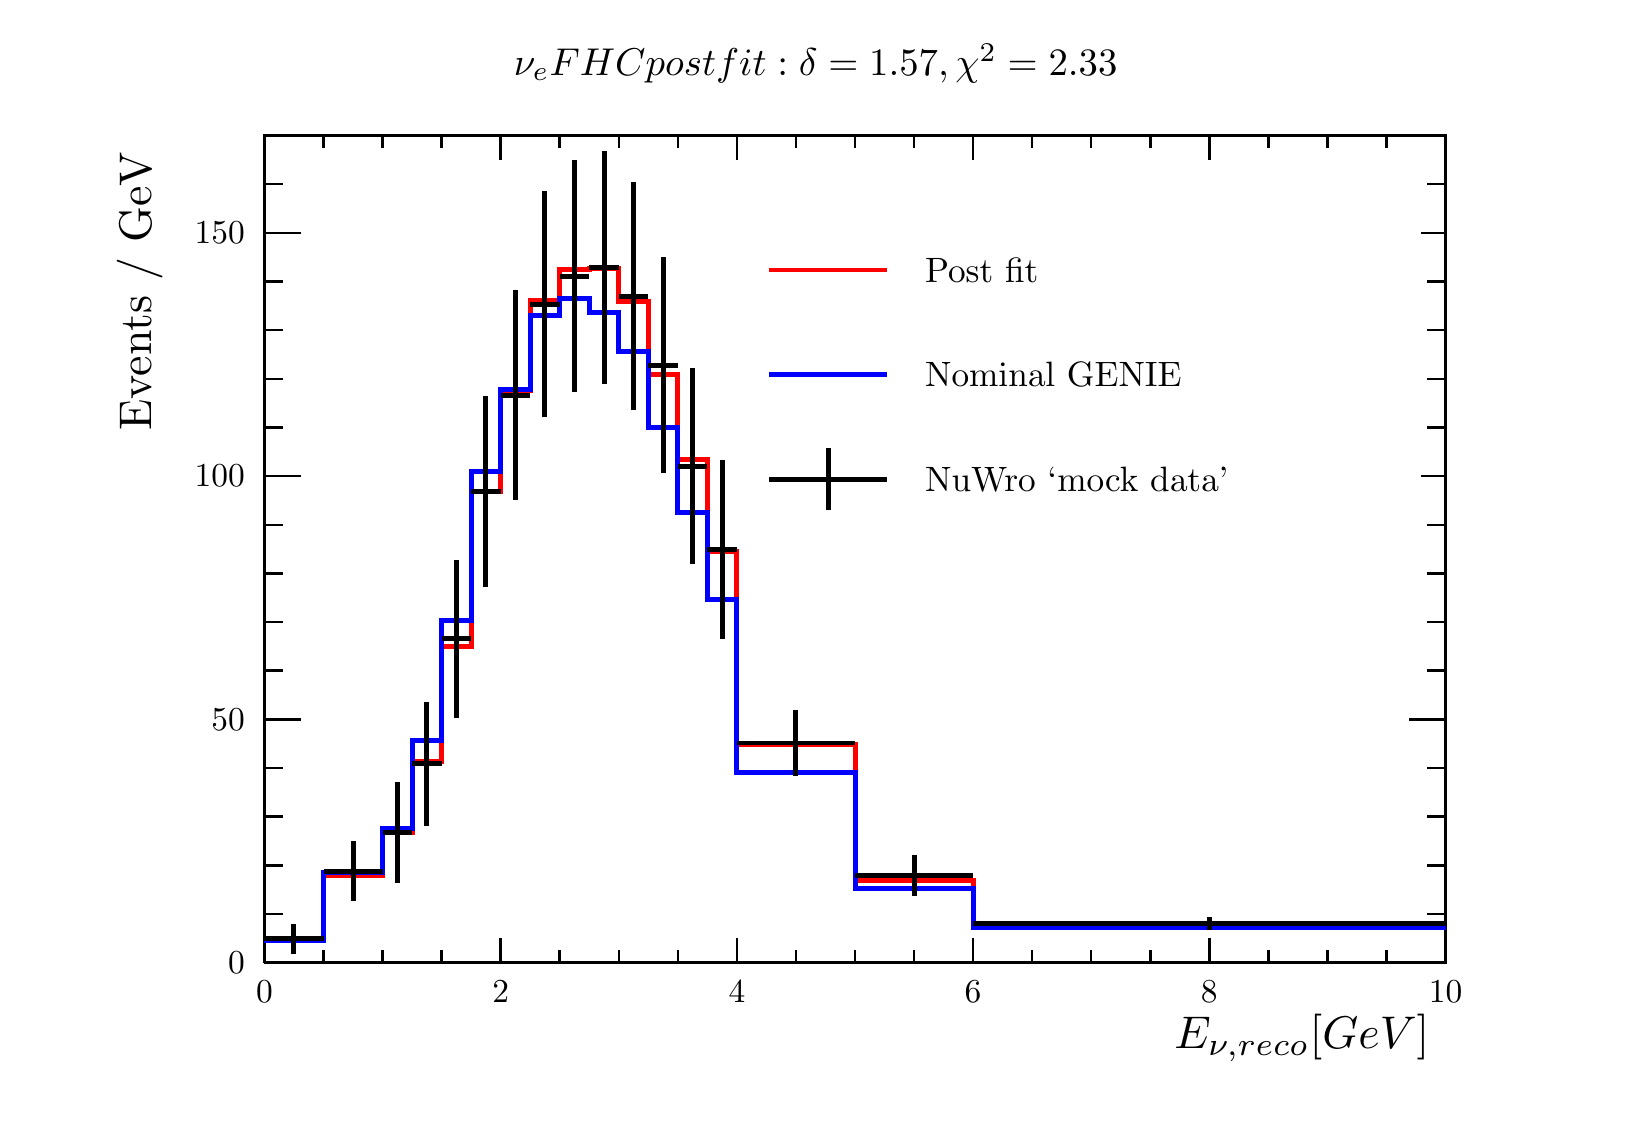
\begin{tikzpicture}
\pgfdeclareplotmark{cross} {
\pgfpathmoveto{\pgfpoint{-0.3\pgfplotmarksize}{\pgfplotmarksize}}
\pgfpathlineto{\pgfpoint{+0.3\pgfplotmarksize}{\pgfplotmarksize}}
\pgfpathlineto{\pgfpoint{+0.3\pgfplotmarksize}{0.3\pgfplotmarksize}}
\pgfpathlineto{\pgfpoint{+1\pgfplotmarksize}{0.3\pgfplotmarksize}}
\pgfpathlineto{\pgfpoint{+1\pgfplotmarksize}{-0.3\pgfplotmarksize}}
\pgfpathlineto{\pgfpoint{+0.3\pgfplotmarksize}{-0.3\pgfplotmarksize}}
\pgfpathlineto{\pgfpoint{+0.3\pgfplotmarksize}{-1.\pgfplotmarksize}}
\pgfpathlineto{\pgfpoint{-0.3\pgfplotmarksize}{-1.\pgfplotmarksize}}
\pgfpathlineto{\pgfpoint{-0.3\pgfplotmarksize}{-0.3\pgfplotmarksize}}
\pgfpathlineto{\pgfpoint{-1.\pgfplotmarksize}{-0.3\pgfplotmarksize}}
\pgfpathlineto{\pgfpoint{-1.\pgfplotmarksize}{0.3\pgfplotmarksize}}
\pgfpathlineto{\pgfpoint{-0.3\pgfplotmarksize}{0.3\pgfplotmarksize}}
\pgfpathclose
\pgfusepathqstroke
}
\pgfdeclareplotmark{cross*} {
\pgfpathmoveto{\pgfpoint{-0.3\pgfplotmarksize}{\pgfplotmarksize}}
\pgfpathlineto{\pgfpoint{+0.3\pgfplotmarksize}{\pgfplotmarksize}}
\pgfpathlineto{\pgfpoint{+0.3\pgfplotmarksize}{0.3\pgfplotmarksize}}
\pgfpathlineto{\pgfpoint{+1\pgfplotmarksize}{0.3\pgfplotmarksize}}
\pgfpathlineto{\pgfpoint{+1\pgfplotmarksize}{-0.3\pgfplotmarksize}}
\pgfpathlineto{\pgfpoint{+0.3\pgfplotmarksize}{-0.3\pgfplotmarksize}}
\pgfpathlineto{\pgfpoint{+0.3\pgfplotmarksize}{-1.\pgfplotmarksize}}
\pgfpathlineto{\pgfpoint{-0.3\pgfplotmarksize}{-1.\pgfplotmarksize}}
\pgfpathlineto{\pgfpoint{-0.3\pgfplotmarksize}{-0.3\pgfplotmarksize}}
\pgfpathlineto{\pgfpoint{-1.\pgfplotmarksize}{-0.3\pgfplotmarksize}}
\pgfpathlineto{\pgfpoint{-1.\pgfplotmarksize}{0.3\pgfplotmarksize}}
\pgfpathlineto{\pgfpoint{-0.3\pgfplotmarksize}{0.3\pgfplotmarksize}}
\pgfpathclose
\pgfusepathqfillstroke
}
\pgfdeclareplotmark{newstar} {
\pgfpathmoveto{\pgfqpoint{0pt}{\pgfplotmarksize}}
\pgfpathlineto{\pgfqpointpolar{44}{0.5\pgfplotmarksize}}
\pgfpathlineto{\pgfqpointpolar{18}{\pgfplotmarksize}}
\pgfpathlineto{\pgfqpointpolar{-20}{0.5\pgfplotmarksize}}
\pgfpathlineto{\pgfqpointpolar{-54}{\pgfplotmarksize}}
\pgfpathlineto{\pgfqpointpolar{-90}{0.5\pgfplotmarksize}}
\pgfpathlineto{\pgfqpointpolar{234}{\pgfplotmarksize}}
\pgfpathlineto{\pgfqpointpolar{198}{0.5\pgfplotmarksize}}
\pgfpathlineto{\pgfqpointpolar{162}{\pgfplotmarksize}}
\pgfpathlineto{\pgfqpointpolar{134}{0.5\pgfplotmarksize}}
\pgfpathclose
\pgfusepathqstroke
}
\pgfdeclareplotmark{newstar*} {
\pgfpathmoveto{\pgfqpoint{0pt}{\pgfplotmarksize}}
\pgfpathlineto{\pgfqpointpolar{44}{0.5\pgfplotmarksize}}
\pgfpathlineto{\pgfqpointpolar{18}{\pgfplotmarksize}}
\pgfpathlineto{\pgfqpointpolar{-20}{0.5\pgfplotmarksize}}
\pgfpathlineto{\pgfqpointpolar{-54}{\pgfplotmarksize}}
\pgfpathlineto{\pgfqpointpolar{-90}{0.5\pgfplotmarksize}}
\pgfpathlineto{\pgfqpointpolar{234}{\pgfplotmarksize}}
\pgfpathlineto{\pgfqpointpolar{198}{0.5\pgfplotmarksize}}
\pgfpathlineto{\pgfqpointpolar{162}{\pgfplotmarksize}}
\pgfpathlineto{\pgfqpointpolar{134}{0.5\pgfplotmarksize}}
\pgfpathclose
\pgfusepathqfillstroke
}
\definecolor{c}{rgb}{1,1,1};
\draw [color=c, fill=c] (0,0) rectangle (20,13.639);
\draw [color=c, fill=c] (3,1.77307) rectangle (18,12.2751);
\definecolor{c}{rgb}{0,0,0};
\draw [c,line width=0.9] (3,1.77307) -- (3,12.2751) -- (18,12.2751) -- (18,1.77307) -- (3,1.77307);
\definecolor{c}{rgb}{1,1,1};
\draw [color=c, fill=c] (3,1.77307) rectangle (18,12.2751);
\definecolor{c}{rgb}{0,0,0};
\draw [c,line width=0.9] (3,1.77307) -- (3,12.2751) -- (18,12.2751) -- (18,1.77307) -- (3,1.77307);
\definecolor{c}{rgb}{1,0,0};
\draw [c,line width=1.8] (3,2.059) -- (3.75,2.059) -- (3.75,2.87639) -- (4.5,2.87639) -- (4.5,3.42495) -- (4.875,3.42495) -- (4.875,4.33215) -- (5.25,4.33215) -- (5.25,5.78427) -- (5.625,5.78427) -- (5.625,7.76137) -- (6,7.76137) -- (6,9.04359) --
 (6.375,9.04359) -- (6.375,10.1806) -- (6.75,10.1806) -- (6.75,10.5725) -- (7.125,10.5725) -- (7.125,10.5838) -- (7.5,10.5838) -- (7.5,10.1744) -- (7.875,10.1744) -- (7.875,9.23699) -- (8.25,9.23699) -- (8.25,8.16016) -- (8.625,8.16016) --
 (8.625,6.99668) -- (9,6.99668) -- (9,4.54455) -- (10.5,4.54455) -- (10.5,2.81665) -- (12,2.81665) -- (12,2.25012) -- (18,2.25012);
\definecolor{c}{rgb}{0,0,0};
\draw [c,line width=0.9] (3,1.77307) -- (18,1.77307);
\draw [c,line width=0.9] (3,2.07994) -- (3,1.77307);
\draw [c,line width=0.9] (3.75,1.9265) -- (3.75,1.77307);
\draw [c,line width=0.9] (4.5,1.9265) -- (4.5,1.77307);
\draw [c,line width=0.9] (5.25,1.9265) -- (5.25,1.77307);
\draw [c,line width=0.9] (6,2.07994) -- (6,1.77307);
\draw [c,line width=0.9] (6.75,1.9265) -- (6.75,1.77307);
\draw [c,line width=0.9] (7.5,1.9265) -- (7.5,1.77307);
\draw [c,line width=0.9] (8.25,1.9265) -- (8.25,1.77307);
\draw [c,line width=0.9] (9,2.07994) -- (9,1.77307);
\draw [c,line width=0.9] (9.75,1.9265) -- (9.75,1.77307);
\draw [c,line width=0.9] (10.5,1.9265) -- (10.5,1.77307);
\draw [c,line width=0.9] (11.25,1.9265) -- (11.25,1.77307);
\draw [c,line width=0.9] (12,2.07994) -- (12,1.77307);
\draw [c,line width=0.9] (12.75,1.9265) -- (12.75,1.77307);
\draw [c,line width=0.9] (13.5,1.9265) -- (13.5,1.77307);
\draw [c,line width=0.9] (14.25,1.9265) -- (14.25,1.77307);
\draw [c,line width=0.9] (15,2.07994) -- (15,1.77307);
\draw [c,line width=0.9] (15.75,1.9265) -- (15.75,1.77307);
\draw [c,line width=0.9] (16.5,1.9265) -- (16.5,1.77307);
\draw [c,line width=0.9] (17.25,1.9265) -- (17.25,1.77307);
\draw [c,line width=0.9] (18,2.07994) -- (18,1.77307);
\draw [anchor=base] (3,1.26842) node[scale=1.20912, color=c, rotate=0]{0};
\draw [anchor=base] (6,1.26842) node[scale=1.20912, color=c, rotate=0]{2};
\draw [anchor=base] (9,1.26842) node[scale=1.20912, color=c, rotate=0]{4};
\draw [anchor=base] (12,1.26842) node[scale=1.20912, color=c, rotate=0]{6};
\draw [anchor=base] (15,1.26842) node[scale=1.20912, color=c, rotate=0]{8};
\draw [anchor=base] (18,1.26842) node[scale=1.20912, color=c, rotate=0]{10};
\draw [anchor= east] (18,0.812882) node[scale=1.65459, color=c, rotate=0]{$E_{\nu, reco} [GeV]$};
\draw [c,line width=0.9] (3,12.2751) -- (18,12.2751);
\draw [c,line width=0.9] (3,11.9682) -- (3,12.2751);
\draw [c,line width=0.9] (3.75,12.1216) -- (3.75,12.2751);
\draw [c,line width=0.9] (4.5,12.1216) -- (4.5,12.2751);
\draw [c,line width=0.9] (5.25,12.1216) -- (5.25,12.2751);
\draw [c,line width=0.9] (6,11.9682) -- (6,12.2751);
\draw [c,line width=0.9] (6.75,12.1216) -- (6.75,12.2751);
\draw [c,line width=0.9] (7.5,12.1216) -- (7.5,12.2751);
\draw [c,line width=0.9] (8.25,12.1216) -- (8.25,12.2751);
\draw [c,line width=0.9] (9,11.9682) -- (9,12.2751);
\draw [c,line width=0.9] (9.75,12.1216) -- (9.75,12.2751);
\draw [c,line width=0.9] (10.5,12.1216) -- (10.5,12.2751);
\draw [c,line width=0.9] (11.25,12.1216) -- (11.25,12.2751);
\draw [c,line width=0.9] (12,11.9682) -- (12,12.2751);
\draw [c,line width=0.9] (12.75,12.1216) -- (12.75,12.2751);
\draw [c,line width=0.9] (13.5,12.1216) -- (13.5,12.2751);
\draw [c,line width=0.9] (14.25,12.1216) -- (14.25,12.2751);
\draw [c,line width=0.9] (15,11.9682) -- (15,12.2751);
\draw [c,line width=0.9] (15.75,12.1216) -- (15.75,12.2751);
\draw [c,line width=0.9] (16.5,12.1216) -- (16.5,12.2751);
\draw [c,line width=0.9] (17.25,12.1216) -- (17.25,12.2751);
\draw [c,line width=0.9] (18,11.9682) -- (18,12.2751);
\draw [c,line width=0.9] (3,1.77307) -- (3,12.2751);
\draw [c,line width=0.9] (3.462,1.77307) -- (3,1.77307);
\draw [c,line width=0.9] (3.231,2.39083) -- (3,2.39083);
\draw [c,line width=0.9] (3.231,3.0086) -- (3,3.0086);
\draw [c,line width=0.9] (3.231,3.62636) -- (3,3.62636);
\draw [c,line width=0.9] (3.231,4.24413) -- (3,4.24413);
\draw [c,line width=0.9] (3.462,4.86189) -- (3,4.86189);
\draw [c,line width=0.9] (3.231,5.47966) -- (3,5.47966);
\draw [c,line width=0.9] (3.231,6.09742) -- (3,6.09742);
\draw [c,line width=0.9] (3.231,6.71519) -- (3,6.71519);
\draw [c,line width=0.9] (3.231,7.33295) -- (3,7.33295);
\draw [c,line width=0.9] (3.462,7.95072) -- (3,7.95072);
\draw [c,line width=0.9] (3.231,8.56848) -- (3,8.56848);
\draw [c,line width=0.9] (3.231,9.18625) -- (3,9.18625);
\draw [c,line width=0.9] (3.231,9.80401) -- (3,9.80401);
\draw [c,line width=0.9] (3.231,10.4218) -- (3,10.4218);
\draw [c,line width=0.9] (3.462,11.0395) -- (3,11.0395);
\draw [c,line width=0.9] (3.462,11.0395) -- (3,11.0395);
\draw [c,line width=0.9] (3.231,11.6573) -- (3,11.6573);
\draw [c,line width=0.9] (3.231,12.2751) -- (3,12.2751);
\draw [anchor= east] (2.9,1.77307) node[scale=1.20912, color=c, rotate=0]{0};
\draw [anchor= east] (2.9,4.86189) node[scale=1.20912, color=c, rotate=0]{50};
\draw [anchor= east] (2.9,7.95072) node[scale=1.20912, color=c, rotate=0]{100};
\draw [anchor= east] (2.9,11.0395) node[scale=1.20912, color=c, rotate=0]{150};
\draw [anchor= east] (1.416,12.2751) node[scale=1.65459, color=c, rotate=90]{Events / GeV};
\draw [c,line width=0.9] (18,1.77307) -- (18,12.2751);
\draw [c,line width=0.9] (17.538,1.77307) -- (18,1.77307);
\draw [c,line width=0.9] (17.769,2.39083) -- (18,2.39083);
\draw [c,line width=0.9] (17.769,3.0086) -- (18,3.0086);
\draw [c,line width=0.9] (17.769,3.62636) -- (18,3.62636);
\draw [c,line width=0.9] (17.769,4.24413) -- (18,4.24413);
\draw [c,line width=0.9] (17.538,4.86189) -- (18,4.86189);
\draw [c,line width=0.9] (17.769,5.47966) -- (18,5.47966);
\draw [c,line width=0.9] (17.769,6.09742) -- (18,6.09742);
\draw [c,line width=0.9] (17.769,6.71519) -- (18,6.71519);
\draw [c,line width=0.9] (17.769,7.33295) -- (18,7.33295);
\draw [c,line width=0.9] (17.538,7.95072) -- (18,7.95072);
\draw [c,line width=0.9] (17.769,8.56848) -- (18,8.56848);
\draw [c,line width=0.9] (17.769,9.18625) -- (18,9.18625);
\draw [c,line width=0.9] (17.769,9.80401) -- (18,9.80401);
\draw [c,line width=0.9] (17.769,10.4218) -- (18,10.4218);
\draw [c,line width=0.9] (17.538,11.0395) -- (18,11.0395);
\draw [c,line width=0.9] (17.538,11.0395) -- (18,11.0395);
\draw [c,line width=0.9] (17.769,11.6573) -- (18,11.6573);
\draw [c,line width=0.9] (17.769,12.2751) -- (18,12.2751);
\definecolor{c}{rgb}{0,0,1};
\draw [c,line width=1.8] (3,2.05641) -- (3.75,2.05641) -- (3.75,2.91454) -- (4.5,2.91454) -- (4.5,3.47351) -- (4.875,3.47351) -- (4.875,4.59637) -- (5.25,4.59637) -- (5.25,6.11824) -- (5.625,6.11824) -- (5.625,8.00335) -- (6,8.00335) -- (6,9.04493)
 -- (6.375,9.04493) -- (6.375,9.99639) -- (6.75,9.99639) -- (6.75,10.2112) -- (7.125,10.2112) -- (7.125,10.0325) -- (7.5,10.0325) -- (7.5,9.53636) -- (7.875,9.53636) -- (7.875,8.57037) -- (8.25,8.57037) -- (8.25,7.48969) -- (8.625,7.48969) --
 (8.625,6.38331) -- (9,6.38331) -- (9,4.18909) -- (10.5,4.18909) -- (10.5,2.71623) -- (12,2.71623) -- (12,2.21727) -- (18,2.21727);
\definecolor{c}{rgb}{0,0,0};
\draw [c,line width=1.8] (3.375,1.88152) -- (3.375,2.07451);
\draw [c,line width=1.8] (3.375,2.07451) -- (3.375,2.26749);
\draw [c,line width=1.8] (3,2.07451) -- (3.375,2.07451);
\draw [c,line width=1.8] (3.375,2.07451) -- (3.75,2.07451);
\foreach \P in {(3.375,2.07451)}{\draw[mark options={color=c,fill=c},mark size=2.402402pt, line width=0.000000pt, mark=*,mark size=1pt] plot coordinates {\P};}
\draw [c,line width=1.8] (4.125,2.55512) -- (4.125,2.93382);
\draw [c,line width=1.8] (4.125,2.93382) -- (4.125,3.31252);
\draw [c,line width=1.8] (3.75,2.93382) -- (4.125,2.93382);
\draw [c,line width=1.8] (4.125,2.93382) -- (4.5,2.93382);
\foreach \P in {(4.125,2.93382)}{\draw[mark options={color=c,fill=c},mark size=2.402402pt, line width=0.000000pt, mark=*,mark size=1pt] plot coordinates {\P};}
\draw [c,line width=1.8] (4.6875,2.78708) -- (4.6875,3.42622);
\draw [c,line width=1.8] (4.6875,3.42622) -- (4.6875,4.06536);
\draw [c,line width=1.8] (4.5,3.42622) -- (4.6875,3.42622);
\draw [c,line width=1.8] (4.6875,3.42622) -- (4.875,3.42622);
\foreach \P in {(4.6875,3.42622)}{\draw[mark options={color=c,fill=c},mark size=2.402402pt, line width=0.000000pt, mark=*,mark size=1pt] plot coordinates {\P};}
\draw [c,line width=1.8] (5.0625,3.50808) -- (5.0625,4.29796);
\draw [c,line width=1.8] (5.0625,4.29796) -- (5.0625,5.08784);
\draw [c,line width=1.8] (4.875,4.29796) -- (5.0625,4.29796);
\draw [c,line width=1.8] (5.0625,4.29796) -- (5.25,4.29796);
\foreach \P in {(5.0625,4.29796)}{\draw[mark options={color=c,fill=c},mark size=2.402402pt, line width=0.000000pt, mark=*,mark size=1pt] plot coordinates {\P};}
\draw [c,line width=1.8] (5.4375,4.87477) -- (5.4375,5.88247);
\draw [c,line width=1.8] (5.4375,5.88247) -- (5.4375,6.89017);
\draw [c,line width=1.8] (5.25,5.88247) -- (5.4375,5.88247);
\draw [c,line width=1.8] (5.4375,5.88247) -- (5.625,5.88247);
\foreach \P in {(5.4375,5.88247)}{\draw[mark options={color=c,fill=c},mark size=2.402402pt, line width=0.000000pt, mark=*,mark size=1pt] plot coordinates {\P};}
\draw [c,line width=1.8] (5.8125,6.5417) -- (5.8125,7.75779);
\draw [c,line width=1.8] (5.8125,7.75779) -- (5.8125,8.97387);
\draw [c,line width=1.8] (5.625,7.75779) -- (5.8125,7.75779);
\draw [c,line width=1.8] (5.8125,7.75779) -- (6,7.75779);
\foreach \P in {(5.8125,7.75779)}{\draw[mark options={color=c,fill=c},mark size=2.402402pt, line width=0.000000pt, mark=*,mark size=1pt] plot coordinates {\P};}
\draw [c,line width=1.8] (6.1875,7.6446) -- (6.1875,8.97901);
\draw [c,line width=1.8] (6.1875,8.97901) -- (6.1875,10.3134);
\draw [c,line width=1.8] (6,8.97901) -- (6.1875,8.97901);
\draw [c,line width=1.8] (6.1875,8.97901) -- (6.375,8.97901);
\foreach \P in {(6.1875,8.97901)}{\draw[mark options={color=c,fill=c},mark size=2.402402pt, line width=0.000000pt, mark=*,mark size=1pt] plot coordinates {\P};}
\draw [c,line width=1.8] (6.5625,8.69782) -- (6.5625,10.1353);
\draw [c,line width=1.8] (6.5625,10.1353) -- (6.5625,11.5728);
\draw [c,line width=1.8] (6.375,10.1353) -- (6.5625,10.1353);
\draw [c,line width=1.8] (6.5625,10.1353) -- (6.75,10.1353);
\foreach \P in {(6.5625,10.1353)}{\draw[mark options={color=c,fill=c},mark size=2.402402pt, line width=0.000000pt, mark=*,mark size=1pt] plot coordinates {\P};}
\draw [c,line width=1.8] (6.9375,9.02356) -- (6.9375,10.4913);
\draw [c,line width=1.8] (6.9375,10.4913) -- (6.9375,11.9591);
\draw [c,line width=1.8] (6.75,10.4913) -- (6.9375,10.4913);
\draw [c,line width=1.8] (6.9375,10.4913) -- (7.125,10.4913);
\foreach \P in {(6.9375,10.4913)}{\draw[mark options={color=c,fill=c},mark size=2.402402pt, line width=0.000000pt, mark=*,mark size=1pt] plot coordinates {\P};}
\draw [c,line width=1.8] (7.3125,9.12259) -- (7.3125,10.5994);
\draw [c,line width=1.8] (7.3125,10.5994) -- (7.3125,12.0763);
\draw [c,line width=1.8] (7.125,10.5994) -- (7.3125,10.5994);
\draw [c,line width=1.8] (7.3125,10.5994) -- (7.5,10.5994);
\foreach \P in {(7.3125,10.5994)}{\draw[mark options={color=c,fill=c},mark size=2.402402pt, line width=0.000000pt, mark=*,mark size=1pt] plot coordinates {\P};}
\draw [c,line width=1.8] (7.6875,8.78946) -- (7.6875,10.2355);
\draw [c,line width=1.8] (7.6875,10.2355) -- (7.6875,11.6816);
\draw [c,line width=1.8] (7.5,10.2355) -- (7.6875,10.2355);
\draw [c,line width=1.8] (7.6875,10.2355) -- (7.875,10.2355);
\foreach \P in {(7.6875,10.2355)}{\draw[mark options={color=c,fill=c},mark size=2.402402pt, line width=0.000000pt, mark=*,mark size=1pt] plot coordinates {\P};}
\draw [c,line width=1.8] (8.0625,7.99097) -- (8.0625,9.36021);
\draw [c,line width=1.8] (8.0625,9.36021) -- (8.0625,10.7295);
\draw [c,line width=1.8] (7.875,9.36021) -- (8.0625,9.36021);
\draw [c,line width=1.8] (8.0625,9.36021) -- (8.25,9.36021);
\foreach \P in {(8.0625,9.36021)}{\draw[mark options={color=c,fill=c},mark size=2.402402pt, line width=0.000000pt, mark=*,mark size=1pt] plot coordinates {\P};}
\draw [c,line width=1.8] (8.4375,6.8301) -- (8.4375,8.07833);
\draw [c,line width=1.8] (8.4375,8.07833) -- (8.4375,9.32656);
\draw [c,line width=1.8] (8.25,8.07833) -- (8.4375,8.07833);
\draw [c,line width=1.8] (8.4375,8.07833) -- (8.625,8.07833);
\foreach \P in {(8.4375,8.07833)}{\draw[mark options={color=c,fill=c},mark size=2.402402pt, line width=0.000000pt, mark=*,mark size=1pt] plot coordinates {\P};}
\draw [c,line width=1.8] (8.8125,5.88043) -- (8.8125,7.01898);
\draw [c,line width=1.8] (8.8125,7.01898) -- (8.8125,8.15753);
\draw [c,line width=1.8] (8.625,7.01898) -- (8.8125,7.01898);
\draw [c,line width=1.8] (8.8125,7.01898) -- (9,7.01898);
\foreach \P in {(8.8125,7.01898)}{\draw[mark options={color=c,fill=c},mark size=2.402402pt, line width=0.000000pt, mark=*,mark size=1pt] plot coordinates {\P};}
\draw [c,line width=1.8] (9.75,4.14636) -- (9.75,4.56139);
\draw [c,line width=1.8] (9.75,4.56139) -- (9.75,4.97643);
\draw [c,line width=1.8] (9,4.56139) -- (9.75,4.56139);
\draw [c,line width=1.8] (9.75,4.56139) -- (10.5,4.56139);
\foreach \P in {(9.75,4.56139)}{\draw[mark options={color=c,fill=c},mark size=2.402402pt, line width=0.000000pt, mark=*,mark size=1pt] plot coordinates {\P};}
\draw [c,line width=1.8] (11.25,2.62032) -- (11.25,2.88207);
\draw [c,line width=1.8] (11.25,2.88207) -- (11.25,3.14381);
\draw [c,line width=1.8] (10.5,2.88207) -- (11.25,2.88207);
\draw [c,line width=1.8] (11.25,2.88207) -- (12,2.88207);
\foreach \P in {(11.25,2.88207)}{\draw[mark options={color=c,fill=c},mark size=2.402402pt, line width=0.000000pt, mark=*,mark size=1pt] plot coordinates {\P};}
\draw [c,line width=1.8] (15,2.18065) -- (15,2.26808);
\draw [c,line width=1.8] (15,2.26808) -- (15,2.35552);
\draw [c,line width=1.8] (12,2.26808) -- (15,2.26808);
\draw [c,line width=1.8] (15,2.26808) -- (18,2.26808);
\foreach \P in {(15,2.26808)}{\draw[mark options={color=c,fill=c},mark size=2.402402pt, line width=0.000000pt, mark=*,mark size=1pt] plot coordinates {\P};}
\definecolor{c}{rgb}{1,1,1};
\draw [color=c, fill=c] (2,12.8206) rectangle (18,13.5708);
\definecolor{c}{rgb}{0,0,0};
\draw (10,13.1957) node[scale=1.40004, color=c, rotate=0]{$\nu_{e} FHC postfit: \delta = 1.57, \chi^{2} = 2.33$};
\definecolor{c}{rgb}{1,1,1};
\draw [color=c, fill=c] (9.08309,7.24928) rectangle (17.6791,11.2321);
\definecolor{c}{rgb}{0,0,0};
\draw [anchor= west] (11.2321,10.5683) node[scale=1.27276, color=c, rotate=0]{Post fit};
\definecolor{c}{rgb}{1,0,0};
\draw [c,line width=1.8] (9.40544,10.5683) -- (10.9097,10.5683);
\definecolor{c}{rgb}{0,0,0};
\draw [anchor= west] (11.2321,9.24069) node[scale=1.27276, color=c, rotate=0]{Nominal GENIE};
\definecolor{c}{rgb}{0,0,1};
\draw [c,line width=1.8] (9.40544,9.24069) -- (10.9097,9.24069);
\definecolor{c}{rgb}{0,0,0};
\draw [anchor= west] (11.2321,7.91308) node[scale=1.27276, color=c, rotate=0]{NuWro `mock data'};
\draw [c,line width=1.8] (9.40544,7.91308) -- (10.9097,7.91308);
\draw [c,line width=1.8] (10.1576,7.5148) -- (10.1576,8.31137);
\end{tikzpicture}

		\end{adjustbox}	
		\caption{\nue FHC}	
	\end{subfigure} \\ 
	\begin{subfigure}[t]{0.5\linewidth}
		\begin{adjustbox}{max totalsize=\linewidth, center}
			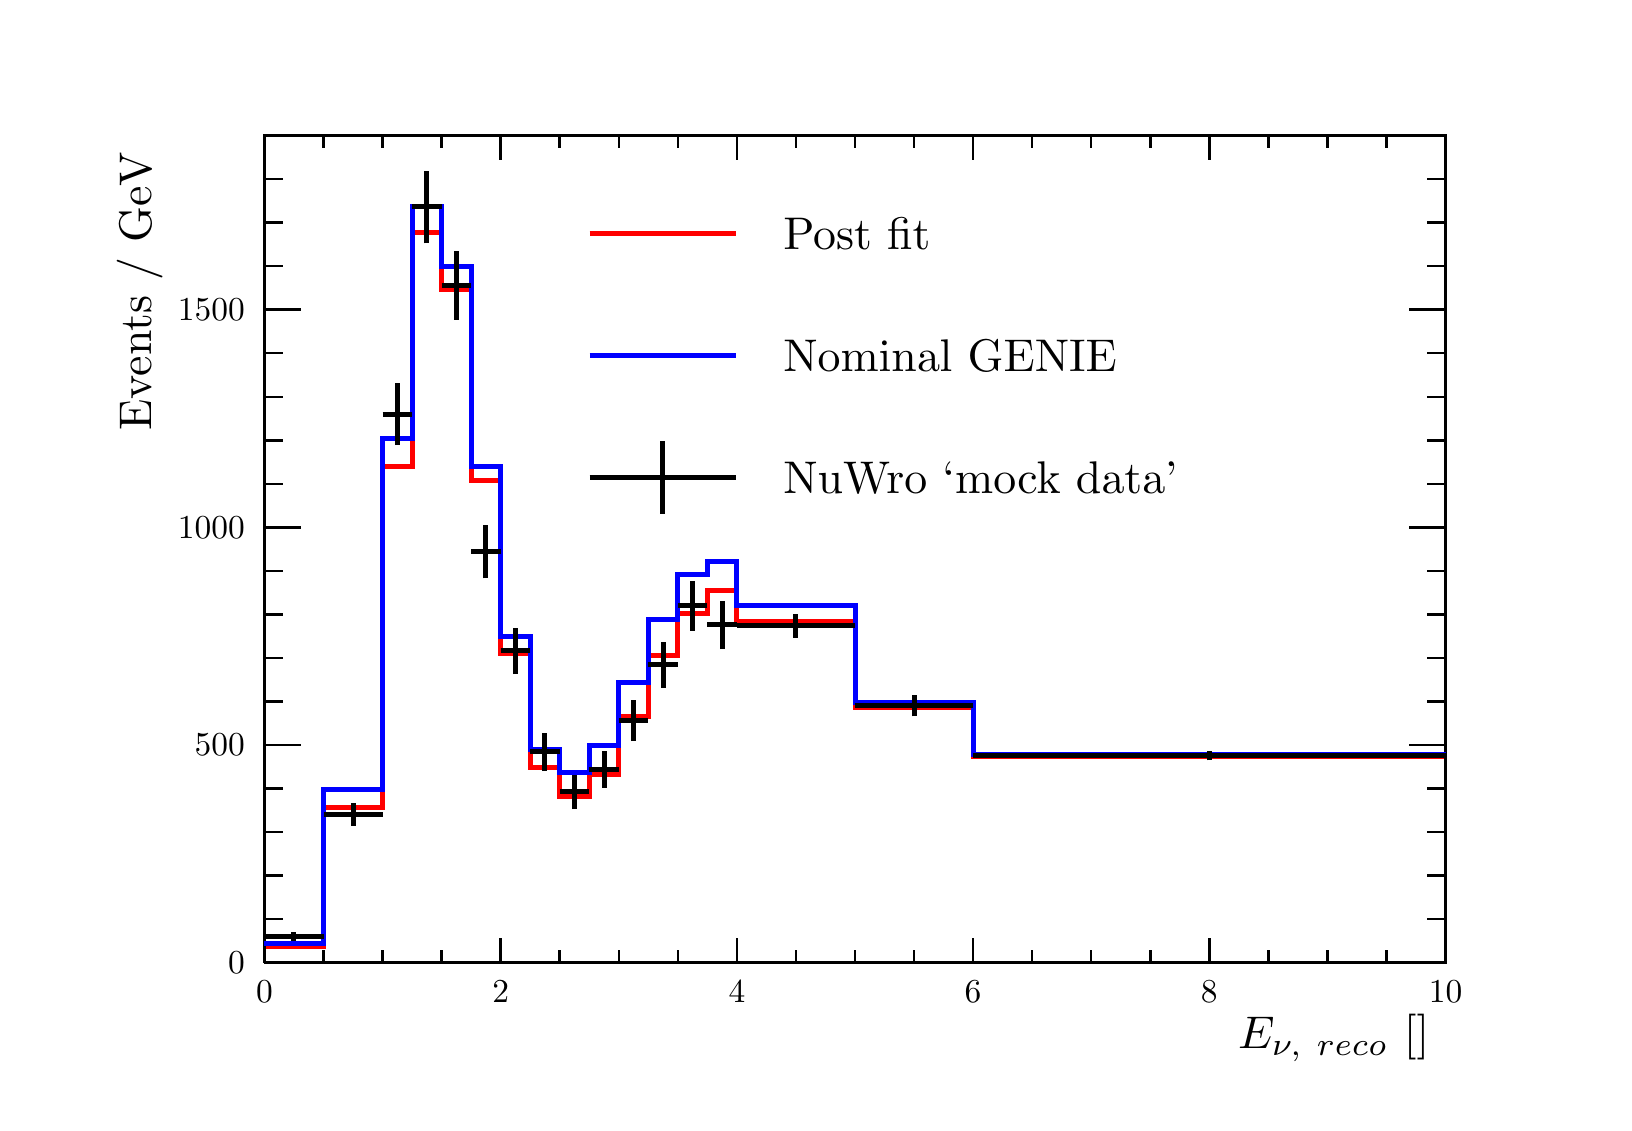
\begin{tikzpicture}
\pgfdeclareplotmark{cross} {
\pgfpathmoveto{\pgfpoint{-0.3\pgfplotmarksize}{\pgfplotmarksize}}
\pgfpathlineto{\pgfpoint{+0.3\pgfplotmarksize}{\pgfplotmarksize}}
\pgfpathlineto{\pgfpoint{+0.3\pgfplotmarksize}{0.3\pgfplotmarksize}}
\pgfpathlineto{\pgfpoint{+1\pgfplotmarksize}{0.3\pgfplotmarksize}}
\pgfpathlineto{\pgfpoint{+1\pgfplotmarksize}{-0.3\pgfplotmarksize}}
\pgfpathlineto{\pgfpoint{+0.3\pgfplotmarksize}{-0.3\pgfplotmarksize}}
\pgfpathlineto{\pgfpoint{+0.3\pgfplotmarksize}{-1.\pgfplotmarksize}}
\pgfpathlineto{\pgfpoint{-0.3\pgfplotmarksize}{-1.\pgfplotmarksize}}
\pgfpathlineto{\pgfpoint{-0.3\pgfplotmarksize}{-0.3\pgfplotmarksize}}
\pgfpathlineto{\pgfpoint{-1.\pgfplotmarksize}{-0.3\pgfplotmarksize}}
\pgfpathlineto{\pgfpoint{-1.\pgfplotmarksize}{0.3\pgfplotmarksize}}
\pgfpathlineto{\pgfpoint{-0.3\pgfplotmarksize}{0.3\pgfplotmarksize}}
\pgfpathclose
\pgfusepathqstroke
}
\pgfdeclareplotmark{cross*} {
\pgfpathmoveto{\pgfpoint{-0.3\pgfplotmarksize}{\pgfplotmarksize}}
\pgfpathlineto{\pgfpoint{+0.3\pgfplotmarksize}{\pgfplotmarksize}}
\pgfpathlineto{\pgfpoint{+0.3\pgfplotmarksize}{0.3\pgfplotmarksize}}
\pgfpathlineto{\pgfpoint{+1\pgfplotmarksize}{0.3\pgfplotmarksize}}
\pgfpathlineto{\pgfpoint{+1\pgfplotmarksize}{-0.3\pgfplotmarksize}}
\pgfpathlineto{\pgfpoint{+0.3\pgfplotmarksize}{-0.3\pgfplotmarksize}}
\pgfpathlineto{\pgfpoint{+0.3\pgfplotmarksize}{-1.\pgfplotmarksize}}
\pgfpathlineto{\pgfpoint{-0.3\pgfplotmarksize}{-1.\pgfplotmarksize}}
\pgfpathlineto{\pgfpoint{-0.3\pgfplotmarksize}{-0.3\pgfplotmarksize}}
\pgfpathlineto{\pgfpoint{-1.\pgfplotmarksize}{-0.3\pgfplotmarksize}}
\pgfpathlineto{\pgfpoint{-1.\pgfplotmarksize}{0.3\pgfplotmarksize}}
\pgfpathlineto{\pgfpoint{-0.3\pgfplotmarksize}{0.3\pgfplotmarksize}}
\pgfpathclose
\pgfusepathqfillstroke
}
\pgfdeclareplotmark{newstar} {
\pgfpathmoveto{\pgfqpoint{0pt}{\pgfplotmarksize}}
\pgfpathlineto{\pgfqpointpolar{44}{0.5\pgfplotmarksize}}
\pgfpathlineto{\pgfqpointpolar{18}{\pgfplotmarksize}}
\pgfpathlineto{\pgfqpointpolar{-20}{0.5\pgfplotmarksize}}
\pgfpathlineto{\pgfqpointpolar{-54}{\pgfplotmarksize}}
\pgfpathlineto{\pgfqpointpolar{-90}{0.5\pgfplotmarksize}}
\pgfpathlineto{\pgfqpointpolar{234}{\pgfplotmarksize}}
\pgfpathlineto{\pgfqpointpolar{198}{0.5\pgfplotmarksize}}
\pgfpathlineto{\pgfqpointpolar{162}{\pgfplotmarksize}}
\pgfpathlineto{\pgfqpointpolar{134}{0.5\pgfplotmarksize}}
\pgfpathclose
\pgfusepathqstroke
}
\pgfdeclareplotmark{newstar*} {
\pgfpathmoveto{\pgfqpoint{0pt}{\pgfplotmarksize}}
\pgfpathlineto{\pgfqpointpolar{44}{0.5\pgfplotmarksize}}
\pgfpathlineto{\pgfqpointpolar{18}{\pgfplotmarksize}}
\pgfpathlineto{\pgfqpointpolar{-20}{0.5\pgfplotmarksize}}
\pgfpathlineto{\pgfqpointpolar{-54}{\pgfplotmarksize}}
\pgfpathlineto{\pgfqpointpolar{-90}{0.5\pgfplotmarksize}}
\pgfpathlineto{\pgfqpointpolar{234}{\pgfplotmarksize}}
\pgfpathlineto{\pgfqpointpolar{198}{0.5\pgfplotmarksize}}
\pgfpathlineto{\pgfqpointpolar{162}{\pgfplotmarksize}}
\pgfpathlineto{\pgfqpointpolar{134}{0.5\pgfplotmarksize}}
\pgfpathclose
\pgfusepathqfillstroke
}
\definecolor{c}{rgb}{1,1,1};
\draw [color=c, fill=c] (0,0) rectangle (20,13.639);
\draw [color=c, fill=c] (3,1.77307) rectangle (18,12.2751);
\definecolor{c}{rgb}{0,0,0};
\draw [c,line width=0.9] (3,1.77307) -- (3,12.2751) -- (18,12.2751) -- (18,1.77307) -- (3,1.77307);
\definecolor{c}{rgb}{1,1,1};
\draw [color=c, fill=c] (3,1.77307) rectangle (18,12.2751);
\definecolor{c}{rgb}{0,0,0};
\draw [c,line width=0.9] (3,1.77307) -- (3,12.2751) -- (18,12.2751) -- (18,1.77307) -- (3,1.77307);
\definecolor{c}{rgb}{1,0,0};
\draw [c,line width=1.8] (3,1.97612) -- (3.75,1.97612) -- (3.75,3.7388) -- (4.5,3.7388) -- (4.5,8.06904) -- (4.875,8.06904) -- (4.875,11.0387) -- (5.25,11.0387) -- (5.25,10.3229) -- (5.625,10.3229) -- (5.625,7.89158) -- (6,7.89158) -- (6,5.69873) --
 (6.375,5.69873) -- (6.375,4.25038) -- (6.75,4.25038) -- (6.75,3.88247) -- (7.125,3.88247) -- (7.125,4.15842) -- (7.5,4.15842) -- (7.5,4.90241) -- (7.875,4.90241) -- (7.875,5.67058) -- (8.25,5.67058) -- (8.25,6.20216) -- (8.625,6.20216) --
 (8.625,6.49336) -- (9,6.49336) -- (9,6.10497) -- (10.5,6.10497) -- (10.5,5.01554) -- (12,5.01554) -- (12,4.39275) -- (18,4.39275);
\definecolor{c}{rgb}{0,0,0};
\draw [c,line width=0.9] (3,1.77307) -- (18,1.77307);
\draw [c,line width=0.9] (3,2.07994) -- (3,1.77307);
\draw [c,line width=0.9] (3.75,1.9265) -- (3.75,1.77307);
\draw [c,line width=0.9] (4.5,1.9265) -- (4.5,1.77307);
\draw [c,line width=0.9] (5.25,1.9265) -- (5.25,1.77307);
\draw [c,line width=0.9] (6,2.07994) -- (6,1.77307);
\draw [c,line width=0.9] (6.75,1.9265) -- (6.75,1.77307);
\draw [c,line width=0.9] (7.5,1.9265) -- (7.5,1.77307);
\draw [c,line width=0.9] (8.25,1.9265) -- (8.25,1.77307);
\draw [c,line width=0.9] (9,2.07994) -- (9,1.77307);
\draw [c,line width=0.9] (9.75,1.9265) -- (9.75,1.77307);
\draw [c,line width=0.9] (10.5,1.9265) -- (10.5,1.77307);
\draw [c,line width=0.9] (11.25,1.9265) -- (11.25,1.77307);
\draw [c,line width=0.9] (12,2.07994) -- (12,1.77307);
\draw [c,line width=0.9] (12.75,1.9265) -- (12.75,1.77307);
\draw [c,line width=0.9] (13.5,1.9265) -- (13.5,1.77307);
\draw [c,line width=0.9] (14.25,1.9265) -- (14.25,1.77307);
\draw [c,line width=0.9] (15,2.07994) -- (15,1.77307);
\draw [c,line width=0.9] (15.75,1.9265) -- (15.75,1.77307);
\draw [c,line width=0.9] (16.5,1.9265) -- (16.5,1.77307);
\draw [c,line width=0.9] (17.25,1.9265) -- (17.25,1.77307);
\draw [c,line width=0.9] (18,2.07994) -- (18,1.77307);
\draw [anchor=base] (3,1.26842) node[scale=1.20912, color=c, rotate=0]{0};
\draw [anchor=base] (6,1.26842) node[scale=1.20912, color=c, rotate=0]{2};
\draw [anchor=base] (9,1.26842) node[scale=1.20912, color=c, rotate=0]{4};
\draw [anchor=base] (12,1.26842) node[scale=1.20912, color=c, rotate=0]{6};
\draw [anchor=base] (15,1.26842) node[scale=1.20912, color=c, rotate=0]{8};
\draw [anchor=base] (18,1.26842) node[scale=1.20912, color=c, rotate=0]{10};
\draw [anchor= east] (18,0.812882) node[scale=1.65459, color=c, rotate=0]{$E_{\nu,~\text{reco}}$ [\si{\GeV}]};
\draw [c,line width=0.9] (3,12.2751) -- (18,12.2751);
\draw [c,line width=0.9] (3,11.9682) -- (3,12.2751);
\draw [c,line width=0.9] (3.75,12.1216) -- (3.75,12.2751);
\draw [c,line width=0.9] (4.5,12.1216) -- (4.5,12.2751);
\draw [c,line width=0.9] (5.25,12.1216) -- (5.25,12.2751);
\draw [c,line width=0.9] (6,11.9682) -- (6,12.2751);
\draw [c,line width=0.9] (6.75,12.1216) -- (6.75,12.2751);
\draw [c,line width=0.9] (7.5,12.1216) -- (7.5,12.2751);
\draw [c,line width=0.9] (8.25,12.1216) -- (8.25,12.2751);
\draw [c,line width=0.9] (9,11.9682) -- (9,12.2751);
\draw [c,line width=0.9] (9.75,12.1216) -- (9.75,12.2751);
\draw [c,line width=0.9] (10.5,12.1216) -- (10.5,12.2751);
\draw [c,line width=0.9] (11.25,12.1216) -- (11.25,12.2751);
\draw [c,line width=0.9] (12,11.9682) -- (12,12.2751);
\draw [c,line width=0.9] (12.75,12.1216) -- (12.75,12.2751);
\draw [c,line width=0.9] (13.5,12.1216) -- (13.5,12.2751);
\draw [c,line width=0.9] (14.25,12.1216) -- (14.25,12.2751);
\draw [c,line width=0.9] (15,11.9682) -- (15,12.2751);
\draw [c,line width=0.9] (15.75,12.1216) -- (15.75,12.2751);
\draw [c,line width=0.9] (16.5,12.1216) -- (16.5,12.2751);
\draw [c,line width=0.9] (17.25,12.1216) -- (17.25,12.2751);
\draw [c,line width=0.9] (18,11.9682) -- (18,12.2751);
\draw [c,line width=0.9] (3,1.77307) -- (3,12.2751);
\draw [c,line width=0.9] (3.462,1.77307) -- (3,1.77307);
\draw [c,line width=0.9] (3.231,2.3258) -- (3,2.3258);
\draw [c,line width=0.9] (3.231,2.87854) -- (3,2.87854);
\draw [c,line width=0.9] (3.231,3.43128) -- (3,3.43128);
\draw [c,line width=0.9] (3.231,3.98401) -- (3,3.98401);
\draw [c,line width=0.9] (3.462,4.53675) -- (3,4.53675);
\draw [c,line width=0.9] (3.231,5.08949) -- (3,5.08949);
\draw [c,line width=0.9] (3.231,5.64223) -- (3,5.64223);
\draw [c,line width=0.9] (3.231,6.19496) -- (3,6.19496);
\draw [c,line width=0.9] (3.231,6.7477) -- (3,6.7477);
\draw [c,line width=0.9] (3.462,7.30044) -- (3,7.30044);
\draw [c,line width=0.9] (3.231,7.85317) -- (3,7.85317);
\draw [c,line width=0.9] (3.231,8.40591) -- (3,8.40591);
\draw [c,line width=0.9] (3.231,8.95865) -- (3,8.95865);
\draw [c,line width=0.9] (3.231,9.51139) -- (3,9.51139);
\draw [c,line width=0.9] (3.462,10.0641) -- (3,10.0641);
\draw [c,line width=0.9] (3.462,10.0641) -- (3,10.0641);
\draw [c,line width=0.9] (3.231,10.6169) -- (3,10.6169);
\draw [c,line width=0.9] (3.231,11.1696) -- (3,11.1696);
\draw [c,line width=0.9] (3.231,11.7223) -- (3,11.7223);
\draw [c,line width=0.9] (3.231,12.2751) -- (3,12.2751);
\draw [anchor= east] (2.9,1.77307) node[scale=1.20912, color=c, rotate=0]{0};
\draw [anchor= east] (2.9,4.53675) node[scale=1.20912, color=c, rotate=0]{500};
\draw [anchor= east] (2.9,7.30044) node[scale=1.20912, color=c, rotate=0]{1000};
\draw [anchor= east] (2.9,10.0641) node[scale=1.20912, color=c, rotate=0]{1500};
\draw [anchor= east] (1.416,12.2751) node[scale=1.65459, color=c, rotate=90]{Events / GeV};
\draw [c,line width=0.9] (18,1.77307) -- (18,12.2751);
\draw [c,line width=0.9] (17.538,1.77307) -- (18,1.77307);
\draw [c,line width=0.9] (17.769,2.3258) -- (18,2.3258);
\draw [c,line width=0.9] (17.769,2.87854) -- (18,2.87854);
\draw [c,line width=0.9] (17.769,3.43128) -- (18,3.43128);
\draw [c,line width=0.9] (17.769,3.98401) -- (18,3.98401);
\draw [c,line width=0.9] (17.538,4.53675) -- (18,4.53675);
\draw [c,line width=0.9] (17.769,5.08949) -- (18,5.08949);
\draw [c,line width=0.9] (17.769,5.64223) -- (18,5.64223);
\draw [c,line width=0.9] (17.769,6.19496) -- (18,6.19496);
\draw [c,line width=0.9] (17.769,6.7477) -- (18,6.7477);
\draw [c,line width=0.9] (17.538,7.30044) -- (18,7.30044);
\draw [c,line width=0.9] (17.769,7.85317) -- (18,7.85317);
\draw [c,line width=0.9] (17.769,8.40591) -- (18,8.40591);
\draw [c,line width=0.9] (17.769,8.95865) -- (18,8.95865);
\draw [c,line width=0.9] (17.769,9.51139) -- (18,9.51139);
\draw [c,line width=0.9] (17.538,10.0641) -- (18,10.0641);
\draw [c,line width=0.9] (17.538,10.0641) -- (18,10.0641);
\draw [c,line width=0.9] (17.769,10.6169) -- (18,10.6169);
\draw [c,line width=0.9] (17.769,11.1696) -- (18,11.1696);
\draw [c,line width=0.9] (17.769,11.7223) -- (18,11.7223);
\draw [c,line width=0.9] (17.769,12.2751) -- (18,12.2751);
\definecolor{c}{rgb}{0,0,1};
\draw [c,line width=1.8] (3,2.01055) -- (3.75,2.01055) -- (3.75,3.96457) -- (4.5,3.96457) -- (4.5,8.43143) -- (4.875,8.43143) -- (4.875,11.3693) -- (5.25,11.3693) -- (5.25,10.609) -- (5.625,10.609) -- (5.625,8.0773) -- (6,8.0773) -- (6,5.91515) --
 (6.375,5.91515) -- (6.375,4.48277) -- (6.75,4.48277) -- (6.75,4.18381) -- (7.125,4.18381) -- (7.125,4.53513) -- (7.5,4.53513) -- (7.5,5.33483) -- (7.875,5.33483) -- (7.875,6.13383) -- (8.25,6.13383) -- (8.25,6.70392) -- (8.625,6.70392) --
 (8.625,6.86182) -- (9,6.86182) -- (9,6.31204) -- (10.5,6.31204) -- (10.5,5.07409) -- (12,5.07409) -- (12,4.41756) -- (18,4.41756);
\definecolor{c}{rgb}{0,0,0};
\draw [c,line width=1.8] (3.375,2.04416) -- (3.375,2.10471);
\draw [c,line width=1.8] (3.375,2.10471) -- (3.375,2.16526);
\draw [c,line width=1.8] (3,2.10471) -- (3.375,2.10471);
\draw [c,line width=1.8] (3.375,2.10471) -- (3.75,2.10471);
\foreach \P in {(3.375,2.10471)}{\draw[mark options={color=c,fill=c},mark size=2.402402pt, line width=0.000000pt, mark=*,mark size=1pt] plot coordinates {\P};}
\draw [c,line width=1.8] (4.125,3.50824) -- (4.125,3.65237);
\draw [c,line width=1.8] (4.125,3.65237) -- (4.125,3.79651);
\draw [c,line width=1.8] (3.75,3.65237) -- (4.125,3.65237);
\draw [c,line width=1.8] (4.125,3.65237) -- (4.5,3.65237);
\foreach \P in {(4.125,3.65237)}{\draw[mark options={color=c,fill=c},mark size=2.402402pt, line width=0.000000pt, mark=*,mark size=1pt] plot coordinates {\P};}
\draw [c,line width=1.8] (4.6875,8.34515) -- (4.6875,8.73755);
\draw [c,line width=1.8] (4.6875,8.73755) -- (4.6875,9.12996);
\draw [c,line width=1.8] (4.5,8.73755) -- (4.6875,8.73755);
\draw [c,line width=1.8] (4.6875,8.73755) -- (4.875,8.73755);
\foreach \P in {(4.6875,8.73755)}{\draw[mark options={color=c,fill=c},mark size=2.402402pt, line width=0.000000pt, mark=*,mark size=1pt] plot coordinates {\P};}
\draw [c,line width=1.8] (5.0625,10.908) -- (5.0625,11.3686);
\draw [c,line width=1.8] (5.0625,11.3686) -- (5.0625,11.8292);
\draw [c,line width=1.8] (4.875,11.3686) -- (5.0625,11.3686);
\draw [c,line width=1.8] (5.0625,11.3686) -- (5.25,11.3686);
\foreach \P in {(5.0625,11.3686)}{\draw[mark options={color=c,fill=c},mark size=2.402402pt, line width=0.000000pt, mark=*,mark size=1pt] plot coordinates {\P};}
\draw [c,line width=1.8] (5.4375,9.93759) -- (5.4375,10.3737);
\draw [c,line width=1.8] (5.4375,10.3737) -- (5.4375,10.8097);
\draw [c,line width=1.8] (5.25,10.3737) -- (5.4375,10.3737);
\draw [c,line width=1.8] (5.4375,10.3737) -- (5.625,10.3737);
\foreach \P in {(5.4375,10.3737)}{\draw[mark options={color=c,fill=c},mark size=2.402402pt, line width=0.000000pt, mark=*,mark size=1pt] plot coordinates {\P};}
\draw [c,line width=1.8] (5.8125,6.65125) -- (5.8125,6.9909);
\draw [c,line width=1.8] (5.8125,6.9909) -- (5.8125,7.33056);
\draw [c,line width=1.8] (5.625,6.9909) -- (5.8125,6.9909);
\draw [c,line width=1.8] (5.8125,6.9909) -- (6,6.9909);
\foreach \P in {(5.8125,6.9909)}{\draw[mark options={color=c,fill=c},mark size=2.402402pt, line width=0.000000pt, mark=*,mark size=1pt] plot coordinates {\P};}
\draw [c,line width=1.8] (6.1875,5.43486) -- (6.1875,5.73066);
\draw [c,line width=1.8] (6.1875,5.73066) -- (6.1875,6.02647);
\draw [c,line width=1.8] (6,5.73066) -- (6.1875,5.73066);
\draw [c,line width=1.8] (6.1875,5.73066) -- (6.375,5.73066);
\foreach \P in {(6.1875,5.73066)}{\draw[mark options={color=c,fill=c},mark size=2.402402pt, line width=0.000000pt, mark=*,mark size=1pt] plot coordinates {\P};}
\draw [c,line width=1.8] (6.5625,4.20511) -- (6.5625,4.44831);
\draw [c,line width=1.8] (6.5625,4.44831) -- (6.5625,4.69152);
\draw [c,line width=1.8] (6.375,4.44831) -- (6.5625,4.44831);
\draw [c,line width=1.8] (6.5625,4.44831) -- (6.75,4.44831);
\foreach \P in {(6.5625,4.44831)}{\draw[mark options={color=c,fill=c},mark size=2.402402pt, line width=0.000000pt, mark=*,mark size=1pt] plot coordinates {\P};}
\draw [c,line width=1.8] (6.9375,3.72092) -- (6.9375,3.9398);
\draw [c,line width=1.8] (6.9375,3.9398) -- (6.9375,4.15867);
\draw [c,line width=1.8] (6.75,3.9398) -- (6.9375,3.9398);
\draw [c,line width=1.8] (6.9375,3.9398) -- (7.125,3.9398);
\foreach \P in {(6.9375,3.9398)}{\draw[mark options={color=c,fill=c},mark size=2.402402pt, line width=0.000000pt, mark=*,mark size=1pt] plot coordinates {\P};}
\draw [c,line width=1.8] (7.3125,3.99428) -- (7.3125,4.22722);
\draw [c,line width=1.8] (7.3125,4.22722) -- (7.3125,4.46016);
\draw [c,line width=1.8] (7.125,4.22722) -- (7.3125,4.22722);
\draw [c,line width=1.8] (7.3125,4.22722) -- (7.5,4.22722);
\foreach \P in {(7.3125,4.22722)}{\draw[mark options={color=c,fill=c},mark size=2.402402pt, line width=0.000000pt, mark=*,mark size=1pt] plot coordinates {\P};}
\draw [c,line width=1.8] (7.6875,4.58562) -- (7.6875,4.84628);
\draw [c,line width=1.8] (7.6875,4.84628) -- (7.6875,5.10695);
\draw [c,line width=1.8] (7.5,4.84628) -- (7.6875,4.84628);
\draw [c,line width=1.8] (7.6875,4.84628) -- (7.875,4.84628);
\foreach \P in {(7.6875,4.84628)}{\draw[mark options={color=c,fill=c},mark size=2.402402pt, line width=0.000000pt, mark=*,mark size=1pt] plot coordinates {\P};}
\draw [c,line width=1.8] (8.0625,5.26467) -- (8.0625,5.55379);
\draw [c,line width=1.8] (8.0625,5.55379) -- (8.0625,5.84291);
\draw [c,line width=1.8] (7.875,5.55379) -- (8.0625,5.55379);
\draw [c,line width=1.8] (8.0625,5.55379) -- (8.25,5.55379);
\foreach \P in {(8.0625,5.55379)}{\draw[mark options={color=c,fill=c},mark size=2.402402pt, line width=0.000000pt, mark=*,mark size=1pt] plot coordinates {\P};}
\draw [c,line width=1.8] (8.4375,5.98895) -- (8.4375,6.30551);
\draw [c,line width=1.8] (8.4375,6.30551) -- (8.4375,6.62207);
\draw [c,line width=1.8] (8.25,6.30551) -- (8.4375,6.30551);
\draw [c,line width=1.8] (8.4375,6.30551) -- (8.625,6.30551);
\foreach \P in {(8.4375,6.30551)}{\draw[mark options={color=c,fill=c},mark size=2.402402pt, line width=0.000000pt, mark=*,mark size=1pt] plot coordinates {\P};}
\draw [c,line width=1.8] (8.8125,5.75436) -- (8.8125,6.06231);
\draw [c,line width=1.8] (8.8125,6.06231) -- (8.8125,6.37026);
\draw [c,line width=1.8] (8.625,6.06231) -- (8.8125,6.06231);
\draw [c,line width=1.8] (8.8125,6.06231) -- (9,6.06231);
\foreach \P in {(8.8125,6.06231)}{\draw[mark options={color=c,fill=c},mark size=2.402402pt, line width=0.000000pt, mark=*,mark size=1pt] plot coordinates {\P};}
\draw [c,line width=1.8] (9.75,5.89748) -- (9.75,6.05125);
\draw [c,line width=1.8] (9.75,6.05125) -- (9.75,6.20503);
\draw [c,line width=1.8] (9,6.05125) -- (9.75,6.05125);
\draw [c,line width=1.8] (9.75,6.05125) -- (10.5,6.05125);
\foreach \P in {(9.75,6.05125)}{\draw[mark options={color=c,fill=c},mark size=2.402402pt, line width=0.000000pt, mark=*,mark size=1pt] plot coordinates {\P};}
\draw [c,line width=1.8] (11.25,4.89996) -- (11.25,5.03421);
\draw [c,line width=1.8] (11.25,5.03421) -- (11.25,5.16847);
\draw [c,line width=1.8] (10.5,5.03421) -- (11.25,5.03421);
\draw [c,line width=1.8] (11.25,5.03421) -- (12,5.03421);
\foreach \P in {(11.25,5.03421)}{\draw[mark options={color=c,fill=c},mark size=2.402402pt, line width=0.000000pt, mark=*,mark size=1pt] plot coordinates {\P};}
\draw [c,line width=1.8] (15,4.34107) -- (15,4.40133);
\draw [c,line width=1.8] (15,4.40133) -- (15,4.4616);
\draw [c,line width=1.8] (12,4.40133) -- (15,4.40133);
\draw [c,line width=1.8] (15,4.40133) -- (18,4.40133);
\foreach \P in {(15,4.40133)}{\draw[mark options={color=c,fill=c},mark size=2.402402pt, line width=0.000000pt, mark=*,mark size=1pt] plot coordinates {\P};}
\definecolor{c}{rgb}{1,1,1};
\draw [color=c, fill=c] (2,12.8206) rectangle (18,13.5708);
\definecolor{c}{rgb}{0,0,0};
%\draw (10,13.1957) node[scale=1.40004, color=c, rotate=0]{$\nu_{\mu} RHC postfit: \delta = 1.57, \chi^{2} = 51.36$};
\definecolor{c}{rgb}{1,1,1};
\draw [color=c, fill=c] (6.73352,7.16332) rectangle (17.3352,11.8052);
\definecolor{c}{rgb}{0,0,0};
\draw [anchor= west] (9.38395,11.0315) node[scale=1.65459, color=c, rotate=0]{Post fit};
\definecolor{c}{rgb}{1,0,0};
\draw [c,line width=1.8] (7.13109,11.0315) -- (8.98639,11.0315);
\definecolor{c}{rgb}{0,0,0};
\draw [anchor= west] (9.38395,9.48424) node[scale=1.65459, color=c, rotate=0]{Nominal GENIE};
\definecolor{c}{rgb}{0,0,1};
\draw [c,line width=1.8] (7.13109,9.48424) -- (8.98639,9.48424);
\definecolor{c}{rgb}{0,0,0};
\draw [anchor= west] (9.38395,7.93696) node[scale=1.65459, color=c, rotate=0]{NuWro `mock data'};
\draw [c,line width=1.8] (7.13109,7.93696) -- (8.98639,7.93696);
\draw [c,line width=1.8] (8.05874,7.47278) -- (8.05874,8.40115);
\end{tikzpicture}

		\end{adjustbox}	
		\caption{\numu RHC}	
	\end{subfigure}	
	\hfill
	\begin{subfigure}[t]{0.5\linewidth}
		\begin{adjustbox}{max totalsize=\linewidth, center}
			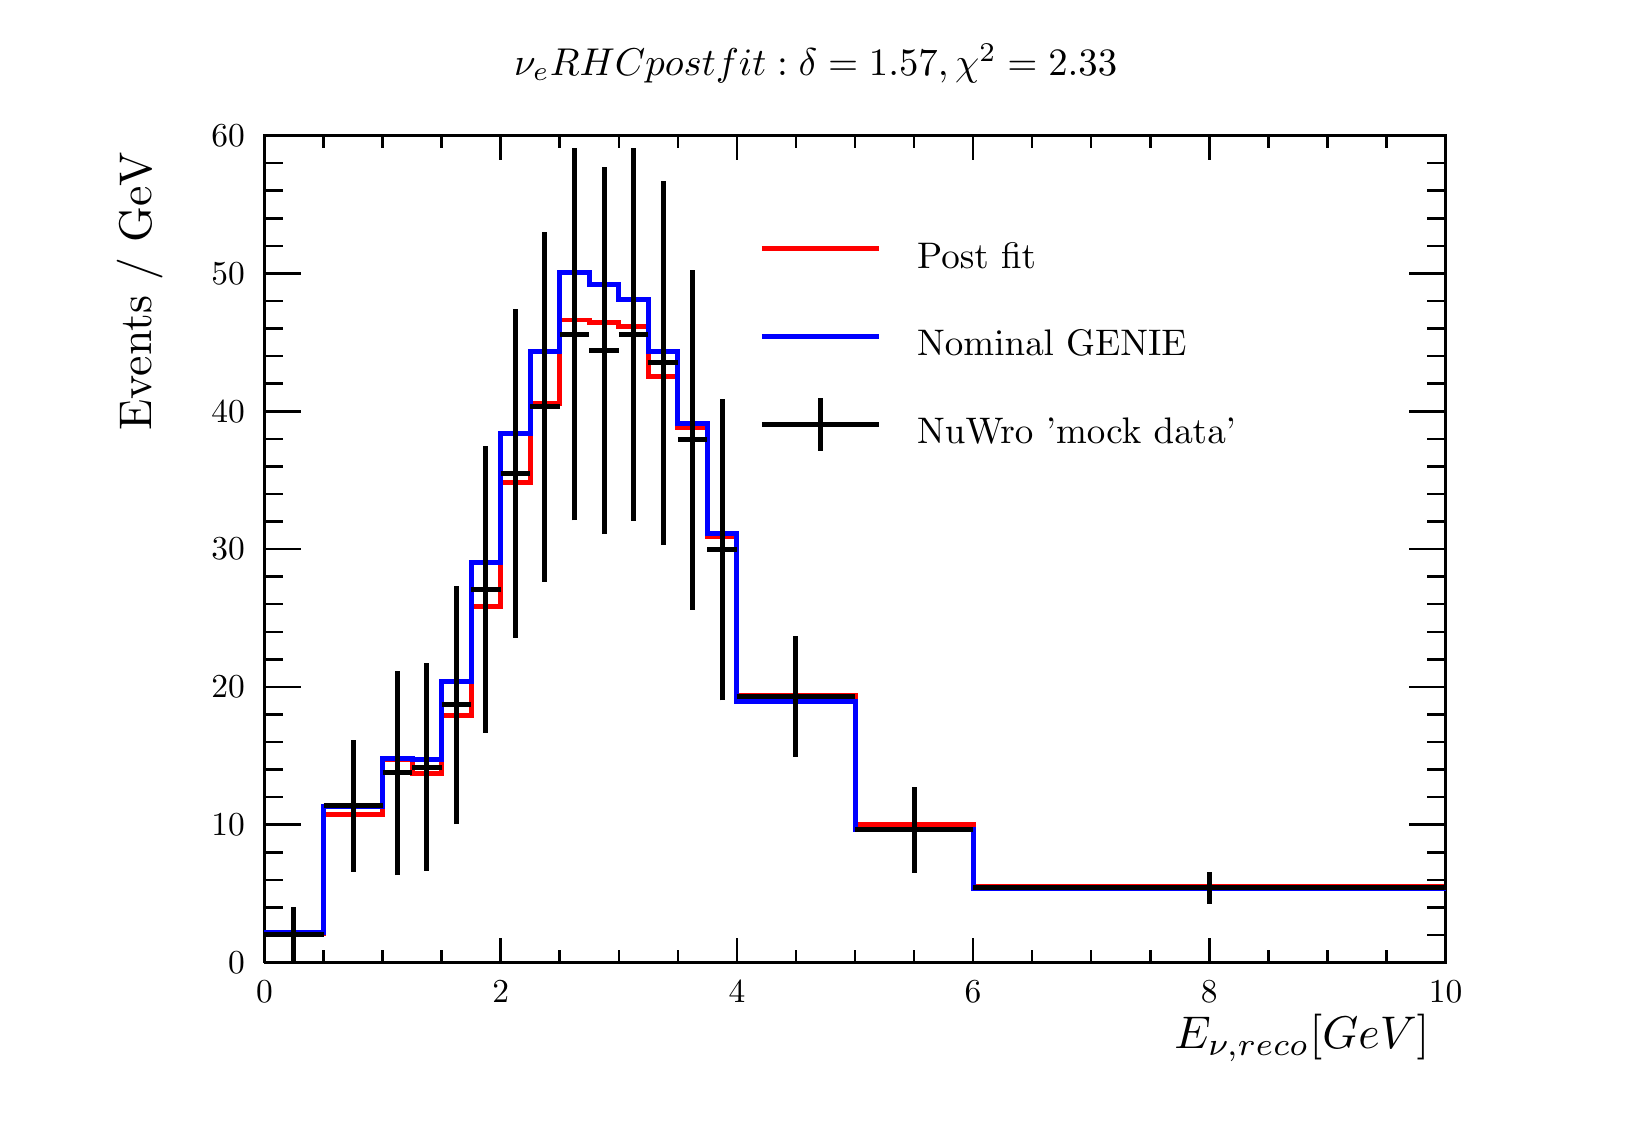
\begin{tikzpicture}
\pgfdeclareplotmark{cross} {
\pgfpathmoveto{\pgfpoint{-0.3\pgfplotmarksize}{\pgfplotmarksize}}
\pgfpathlineto{\pgfpoint{+0.3\pgfplotmarksize}{\pgfplotmarksize}}
\pgfpathlineto{\pgfpoint{+0.3\pgfplotmarksize}{0.3\pgfplotmarksize}}
\pgfpathlineto{\pgfpoint{+1\pgfplotmarksize}{0.3\pgfplotmarksize}}
\pgfpathlineto{\pgfpoint{+1\pgfplotmarksize}{-0.3\pgfplotmarksize}}
\pgfpathlineto{\pgfpoint{+0.3\pgfplotmarksize}{-0.3\pgfplotmarksize}}
\pgfpathlineto{\pgfpoint{+0.3\pgfplotmarksize}{-1.\pgfplotmarksize}}
\pgfpathlineto{\pgfpoint{-0.3\pgfplotmarksize}{-1.\pgfplotmarksize}}
\pgfpathlineto{\pgfpoint{-0.3\pgfplotmarksize}{-0.3\pgfplotmarksize}}
\pgfpathlineto{\pgfpoint{-1.\pgfplotmarksize}{-0.3\pgfplotmarksize}}
\pgfpathlineto{\pgfpoint{-1.\pgfplotmarksize}{0.3\pgfplotmarksize}}
\pgfpathlineto{\pgfpoint{-0.3\pgfplotmarksize}{0.3\pgfplotmarksize}}
\pgfpathclose
\pgfusepathqstroke
}
\pgfdeclareplotmark{cross*} {
\pgfpathmoveto{\pgfpoint{-0.3\pgfplotmarksize}{\pgfplotmarksize}}
\pgfpathlineto{\pgfpoint{+0.3\pgfplotmarksize}{\pgfplotmarksize}}
\pgfpathlineto{\pgfpoint{+0.3\pgfplotmarksize}{0.3\pgfplotmarksize}}
\pgfpathlineto{\pgfpoint{+1\pgfplotmarksize}{0.3\pgfplotmarksize}}
\pgfpathlineto{\pgfpoint{+1\pgfplotmarksize}{-0.3\pgfplotmarksize}}
\pgfpathlineto{\pgfpoint{+0.3\pgfplotmarksize}{-0.3\pgfplotmarksize}}
\pgfpathlineto{\pgfpoint{+0.3\pgfplotmarksize}{-1.\pgfplotmarksize}}
\pgfpathlineto{\pgfpoint{-0.3\pgfplotmarksize}{-1.\pgfplotmarksize}}
\pgfpathlineto{\pgfpoint{-0.3\pgfplotmarksize}{-0.3\pgfplotmarksize}}
\pgfpathlineto{\pgfpoint{-1.\pgfplotmarksize}{-0.3\pgfplotmarksize}}
\pgfpathlineto{\pgfpoint{-1.\pgfplotmarksize}{0.3\pgfplotmarksize}}
\pgfpathlineto{\pgfpoint{-0.3\pgfplotmarksize}{0.3\pgfplotmarksize}}
\pgfpathclose
\pgfusepathqfillstroke
}
\pgfdeclareplotmark{newstar} {
\pgfpathmoveto{\pgfqpoint{0pt}{\pgfplotmarksize}}
\pgfpathlineto{\pgfqpointpolar{44}{0.5\pgfplotmarksize}}
\pgfpathlineto{\pgfqpointpolar{18}{\pgfplotmarksize}}
\pgfpathlineto{\pgfqpointpolar{-20}{0.5\pgfplotmarksize}}
\pgfpathlineto{\pgfqpointpolar{-54}{\pgfplotmarksize}}
\pgfpathlineto{\pgfqpointpolar{-90}{0.5\pgfplotmarksize}}
\pgfpathlineto{\pgfqpointpolar{234}{\pgfplotmarksize}}
\pgfpathlineto{\pgfqpointpolar{198}{0.5\pgfplotmarksize}}
\pgfpathlineto{\pgfqpointpolar{162}{\pgfplotmarksize}}
\pgfpathlineto{\pgfqpointpolar{134}{0.5\pgfplotmarksize}}
\pgfpathclose
\pgfusepathqstroke
}
\pgfdeclareplotmark{newstar*} {
\pgfpathmoveto{\pgfqpoint{0pt}{\pgfplotmarksize}}
\pgfpathlineto{\pgfqpointpolar{44}{0.5\pgfplotmarksize}}
\pgfpathlineto{\pgfqpointpolar{18}{\pgfplotmarksize}}
\pgfpathlineto{\pgfqpointpolar{-20}{0.5\pgfplotmarksize}}
\pgfpathlineto{\pgfqpointpolar{-54}{\pgfplotmarksize}}
\pgfpathlineto{\pgfqpointpolar{-90}{0.5\pgfplotmarksize}}
\pgfpathlineto{\pgfqpointpolar{234}{\pgfplotmarksize}}
\pgfpathlineto{\pgfqpointpolar{198}{0.5\pgfplotmarksize}}
\pgfpathlineto{\pgfqpointpolar{162}{\pgfplotmarksize}}
\pgfpathlineto{\pgfqpointpolar{134}{0.5\pgfplotmarksize}}
\pgfpathclose
\pgfusepathqfillstroke
}
\definecolor{c}{rgb}{1,1,1};
\draw [color=c, fill=c] (0,0) rectangle (20,13.639);
\draw [color=c, fill=c] (3,1.77307) rectangle (18,12.2751);
\definecolor{c}{rgb}{0,0,0};
\draw [c,line width=0.9] (3,1.77307) -- (3,12.2751) -- (18,12.2751) -- (18,1.77307) -- (3,1.77307);
\definecolor{c}{rgb}{1,1,1};
\draw [color=c, fill=c] (3,1.77307) rectangle (18,12.2751);
\definecolor{c}{rgb}{0,0,0};
\draw [c,line width=0.9] (3,1.77307) -- (3,12.2751) -- (18,12.2751) -- (18,1.77307) -- (3,1.77307);
\definecolor{c}{rgb}{1,0,0};
\draw [c,line width=1.8] (3,2.14759) -- (3.75,2.14759) -- (3.75,3.65643) -- (4.5,3.65643) -- (4.5,4.35413) -- (4.875,4.35413) -- (4.875,4.16903) -- (5.25,4.16903) -- (5.25,4.91121) -- (5.625,4.91121) -- (5.625,6.29666) -- (6,6.29666) -- (6,7.87535)
 -- (6.375,7.87535) -- (6.375,8.87477) -- (6.75,8.87477) -- (6.75,9.93327) -- (7.125,9.93327) -- (7.125,9.89581) -- (7.5,9.89581) -- (7.5,9.85087) -- (7.875,9.85087) -- (7.875,9.21101) -- (8.25,9.21101) -- (8.25,8.57305) -- (8.625,8.57305) --
 (8.625,7.17842) -- (9,7.17842) -- (9,5.1658) -- (10.5,5.1658) -- (10.5,3.52174) -- (12,3.52174) -- (12,2.74511) -- (18,2.74511);
\definecolor{c}{rgb}{0,0,0};
\draw [c,line width=0.9] (3,1.77307) -- (18,1.77307);
\draw [c,line width=0.9] (3,2.07994) -- (3,1.77307);
\draw [c,line width=0.9] (3.75,1.9265) -- (3.75,1.77307);
\draw [c,line width=0.9] (4.5,1.9265) -- (4.5,1.77307);
\draw [c,line width=0.9] (5.25,1.9265) -- (5.25,1.77307);
\draw [c,line width=0.9] (6,2.07994) -- (6,1.77307);
\draw [c,line width=0.9] (6.75,1.9265) -- (6.75,1.77307);
\draw [c,line width=0.9] (7.5,1.9265) -- (7.5,1.77307);
\draw [c,line width=0.9] (8.25,1.9265) -- (8.25,1.77307);
\draw [c,line width=0.9] (9,2.07994) -- (9,1.77307);
\draw [c,line width=0.9] (9.75,1.9265) -- (9.75,1.77307);
\draw [c,line width=0.9] (10.5,1.9265) -- (10.5,1.77307);
\draw [c,line width=0.9] (11.25,1.9265) -- (11.25,1.77307);
\draw [c,line width=0.9] (12,2.07994) -- (12,1.77307);
\draw [c,line width=0.9] (12.75,1.9265) -- (12.75,1.77307);
\draw [c,line width=0.9] (13.5,1.9265) -- (13.5,1.77307);
\draw [c,line width=0.9] (14.25,1.9265) -- (14.25,1.77307);
\draw [c,line width=0.9] (15,2.07994) -- (15,1.77307);
\draw [c,line width=0.9] (15.75,1.9265) -- (15.75,1.77307);
\draw [c,line width=0.9] (16.5,1.9265) -- (16.5,1.77307);
\draw [c,line width=0.9] (17.25,1.9265) -- (17.25,1.77307);
\draw [c,line width=0.9] (18,2.07994) -- (18,1.77307);
\draw [anchor=base] (3,1.26842) node[scale=1.20912, color=c, rotate=0]{0};
\draw [anchor=base] (6,1.26842) node[scale=1.20912, color=c, rotate=0]{2};
\draw [anchor=base] (9,1.26842) node[scale=1.20912, color=c, rotate=0]{4};
\draw [anchor=base] (12,1.26842) node[scale=1.20912, color=c, rotate=0]{6};
\draw [anchor=base] (15,1.26842) node[scale=1.20912, color=c, rotate=0]{8};
\draw [anchor=base] (18,1.26842) node[scale=1.20912, color=c, rotate=0]{10};
\draw [anchor= east] (18,0.812882) node[scale=1.65459, color=c, rotate=0]{$E_{\nu, reco} [GeV]$};
\draw [c,line width=0.9] (3,12.2751) -- (18,12.2751);
\draw [c,line width=0.9] (3,11.9682) -- (3,12.2751);
\draw [c,line width=0.9] (3.75,12.1216) -- (3.75,12.2751);
\draw [c,line width=0.9] (4.5,12.1216) -- (4.5,12.2751);
\draw [c,line width=0.9] (5.25,12.1216) -- (5.25,12.2751);
\draw [c,line width=0.9] (6,11.9682) -- (6,12.2751);
\draw [c,line width=0.9] (6.75,12.1216) -- (6.75,12.2751);
\draw [c,line width=0.9] (7.5,12.1216) -- (7.5,12.2751);
\draw [c,line width=0.9] (8.25,12.1216) -- (8.25,12.2751);
\draw [c,line width=0.9] (9,11.9682) -- (9,12.2751);
\draw [c,line width=0.9] (9.75,12.1216) -- (9.75,12.2751);
\draw [c,line width=0.9] (10.5,12.1216) -- (10.5,12.2751);
\draw [c,line width=0.9] (11.25,12.1216) -- (11.25,12.2751);
\draw [c,line width=0.9] (12,11.9682) -- (12,12.2751);
\draw [c,line width=0.9] (12.75,12.1216) -- (12.75,12.2751);
\draw [c,line width=0.9] (13.5,12.1216) -- (13.5,12.2751);
\draw [c,line width=0.9] (14.25,12.1216) -- (14.25,12.2751);
\draw [c,line width=0.9] (15,11.9682) -- (15,12.2751);
\draw [c,line width=0.9] (15.75,12.1216) -- (15.75,12.2751);
\draw [c,line width=0.9] (16.5,12.1216) -- (16.5,12.2751);
\draw [c,line width=0.9] (17.25,12.1216) -- (17.25,12.2751);
\draw [c,line width=0.9] (18,11.9682) -- (18,12.2751);
\draw [c,line width=0.9] (3,1.77307) -- (3,12.2751);
\draw [c,line width=0.9] (3.462,1.77307) -- (3,1.77307);
\draw [c,line width=0.9] (3.231,2.12313) -- (3,2.12313);
\draw [c,line width=0.9] (3.231,2.4732) -- (3,2.4732);
\draw [c,line width=0.9] (3.231,2.82327) -- (3,2.82327);
\draw [c,line width=0.9] (3.231,3.17333) -- (3,3.17333);
\draw [c,line width=0.9] (3.462,3.5234) -- (3,3.5234);
\draw [c,line width=0.9] (3.231,3.87347) -- (3,3.87347);
\draw [c,line width=0.9] (3.231,4.22353) -- (3,4.22353);
\draw [c,line width=0.9] (3.231,4.5736) -- (3,4.5736);
\draw [c,line width=0.9] (3.231,4.92367) -- (3,4.92367);
\draw [c,line width=0.9] (3.462,5.27373) -- (3,5.27373);
\draw [c,line width=0.9] (3.231,5.6238) -- (3,5.6238);
\draw [c,line width=0.9] (3.231,5.97387) -- (3,5.97387);
\draw [c,line width=0.9] (3.231,6.32394) -- (3,6.32394);
\draw [c,line width=0.9] (3.231,6.674) -- (3,6.674);
\draw [c,line width=0.9] (3.462,7.02407) -- (3,7.02407);
\draw [c,line width=0.9] (3.231,7.37414) -- (3,7.37414);
\draw [c,line width=0.9] (3.231,7.7242) -- (3,7.7242);
\draw [c,line width=0.9] (3.231,8.07427) -- (3,8.07427);
\draw [c,line width=0.9] (3.231,8.42434) -- (3,8.42434);
\draw [c,line width=0.9] (3.462,8.7744) -- (3,8.7744);
\draw [c,line width=0.9] (3.231,9.12447) -- (3,9.12447);
\draw [c,line width=0.9] (3.231,9.47454) -- (3,9.47454);
\draw [c,line width=0.9] (3.231,9.8246) -- (3,9.8246);
\draw [c,line width=0.9] (3.231,10.1747) -- (3,10.1747);
\draw [c,line width=0.9] (3.462,10.5247) -- (3,10.5247);
\draw [c,line width=0.9] (3.231,10.8748) -- (3,10.8748);
\draw [c,line width=0.9] (3.231,11.2249) -- (3,11.2249);
\draw [c,line width=0.9] (3.231,11.5749) -- (3,11.5749);
\draw [c,line width=0.9] (3.231,11.925) -- (3,11.925);
\draw [c,line width=0.9] (3.462,12.2751) -- (3,12.2751);
\draw [anchor= east] (2.9,1.77307) node[scale=1.20912, color=c, rotate=0]{0};
\draw [anchor= east] (2.9,3.5234) node[scale=1.20912, color=c, rotate=0]{10};
\draw [anchor= east] (2.9,5.27373) node[scale=1.20912, color=c, rotate=0]{20};
\draw [anchor= east] (2.9,7.02407) node[scale=1.20912, color=c, rotate=0]{30};
\draw [anchor= east] (2.9,8.7744) node[scale=1.20912, color=c, rotate=0]{40};
\draw [anchor= east] (2.9,10.5247) node[scale=1.20912, color=c, rotate=0]{50};
\draw [anchor= east] (2.9,12.2751) node[scale=1.20912, color=c, rotate=0]{60};
\draw [anchor= east] (1.416,12.2751) node[scale=1.65459, color=c, rotate=90]{Events / GeV};
\draw [c,line width=0.9] (18,1.77307) -- (18,12.2751);
\draw [c,line width=0.9] (17.538,1.77307) -- (18,1.77307);
\draw [c,line width=0.9] (17.769,2.12313) -- (18,2.12313);
\draw [c,line width=0.9] (17.769,2.4732) -- (18,2.4732);
\draw [c,line width=0.9] (17.769,2.82327) -- (18,2.82327);
\draw [c,line width=0.9] (17.769,3.17333) -- (18,3.17333);
\draw [c,line width=0.9] (17.538,3.5234) -- (18,3.5234);
\draw [c,line width=0.9] (17.769,3.87347) -- (18,3.87347);
\draw [c,line width=0.9] (17.769,4.22353) -- (18,4.22353);
\draw [c,line width=0.9] (17.769,4.5736) -- (18,4.5736);
\draw [c,line width=0.9] (17.769,4.92367) -- (18,4.92367);
\draw [c,line width=0.9] (17.538,5.27373) -- (18,5.27373);
\draw [c,line width=0.9] (17.769,5.6238) -- (18,5.6238);
\draw [c,line width=0.9] (17.769,5.97387) -- (18,5.97387);
\draw [c,line width=0.9] (17.769,6.32394) -- (18,6.32394);
\draw [c,line width=0.9] (17.769,6.674) -- (18,6.674);
\draw [c,line width=0.9] (17.538,7.02407) -- (18,7.02407);
\draw [c,line width=0.9] (17.769,7.37414) -- (18,7.37414);
\draw [c,line width=0.9] (17.769,7.7242) -- (18,7.7242);
\draw [c,line width=0.9] (17.769,8.07427) -- (18,8.07427);
\draw [c,line width=0.9] (17.769,8.42434) -- (18,8.42434);
\draw [c,line width=0.9] (17.538,8.7744) -- (18,8.7744);
\draw [c,line width=0.9] (17.769,9.12447) -- (18,9.12447);
\draw [c,line width=0.9] (17.769,9.47454) -- (18,9.47454);
\draw [c,line width=0.9] (17.769,9.8246) -- (18,9.8246);
\draw [c,line width=0.9] (17.769,10.1747) -- (18,10.1747);
\draw [c,line width=0.9] (17.538,10.5247) -- (18,10.5247);
\draw [c,line width=0.9] (17.769,10.8748) -- (18,10.8748);
\draw [c,line width=0.9] (17.769,11.2249) -- (18,11.2249);
\draw [c,line width=0.9] (17.769,11.5749) -- (18,11.5749);
\draw [c,line width=0.9] (17.769,11.925) -- (18,11.925);
\draw [c,line width=0.9] (17.538,12.2751) -- (18,12.2751);
\definecolor{c}{rgb}{0,0,1};
\draw [c,line width=1.8] (3,2.15226) -- (3.75,2.15226) -- (3.75,3.75423) -- (4.5,3.75423) -- (4.5,4.36094) -- (4.875,4.36094) -- (4.875,4.35302) -- (5.25,4.35302) -- (5.25,5.34112) -- (5.625,5.34112) -- (5.625,6.85827) -- (6,6.85827) -- (6,8.488) --
 (6.375,8.488) -- (6.375,9.53779) -- (6.75,9.53779) -- (6.75,10.5331) -- (7.125,10.5331) -- (7.125,10.3888) -- (7.5,10.3888) -- (7.5,10.1991) -- (7.875,10.1991) -- (7.875,9.52723) -- (8.25,9.52723) -- (8.25,8.6204) -- (8.625,8.6204) --
 (8.625,7.21893) -- (9,7.21893) -- (9,5.08334) -- (10.5,5.08334) -- (10.5,3.46716) -- (12,3.46716) -- (12,2.70892) -- (18,2.70892);
\definecolor{c}{rgb}{0,0,0};
\draw [c,line width=1.8] (3.375,1.77636) -- (3.375,2.12969);
\draw [c,line width=1.8] (3.375,2.12969) -- (3.375,2.48302);
\draw [c,line width=1.8] (3,2.12969) -- (3.375,2.12969);
\draw [c,line width=1.8] (3.375,2.12969) -- (3.75,2.12969);
\foreach \P in {(3.375,2.12969)}{\draw[mark options={color=c,fill=c},mark size=2.402402pt, line width=0.000000pt, mark=*,mark size=1pt] plot coordinates {\P};}
\draw [c,line width=1.8] (4.125,2.92717) -- (4.125,3.76148);
\draw [c,line width=1.8] (4.125,3.76148) -- (4.125,4.5958);
\draw [c,line width=1.8] (3.75,3.76148) -- (4.125,3.76148);
\draw [c,line width=1.8] (4.125,3.76148) -- (4.5,3.76148);
\foreach \P in {(4.125,3.76148)}{\draw[mark options={color=c,fill=c},mark size=2.402402pt, line width=0.000000pt, mark=*,mark size=1pt] plot coordinates {\P};}
\draw [c,line width=1.8] (4.6875,2.88356) -- (4.6875,4.18233);
\draw [c,line width=1.8] (4.6875,4.18233) -- (4.6875,5.4811);
\draw [c,line width=1.8] (4.5,4.18233) -- (4.6875,4.18233);
\draw [c,line width=1.8] (4.6875,4.18233) -- (4.875,4.18233);
\foreach \P in {(4.6875,4.18233)}{\draw[mark options={color=c,fill=c},mark size=2.402402pt, line width=0.000000pt, mark=*,mark size=1pt] plot coordinates {\P};}
\draw [c,line width=1.8] (5.0625,2.93629) -- (5.0625,4.25432);
\draw [c,line width=1.8] (5.0625,4.25432) -- (5.0625,5.57235);
\draw [c,line width=1.8] (4.875,4.25432) -- (5.0625,4.25432);
\draw [c,line width=1.8] (5.0625,4.25432) -- (5.25,4.25432);
\foreach \P in {(5.0625,4.25432)}{\draw[mark options={color=c,fill=c},mark size=2.402402pt, line width=0.000000pt, mark=*,mark size=1pt] plot coordinates {\P};}
\draw [c,line width=1.8] (5.4375,3.53101) -- (5.4375,5.04441);
\draw [c,line width=1.8] (5.4375,5.04441) -- (5.4375,6.55781);
\draw [c,line width=1.8] (5.25,5.04441) -- (5.4375,5.04441);
\draw [c,line width=1.8] (5.4375,5.04441) -- (5.625,5.04441);
\foreach \P in {(5.4375,5.04441)}{\draw[mark options={color=c,fill=c},mark size=2.402402pt, line width=0.000000pt, mark=*,mark size=1pt] plot coordinates {\P};}
\draw [c,line width=1.8] (5.8125,4.69) -- (5.8125,6.51139);
\draw [c,line width=1.8] (5.8125,6.51139) -- (5.8125,8.33278);
\draw [c,line width=1.8] (5.625,6.51139) -- (5.8125,6.51139);
\draw [c,line width=1.8] (5.8125,6.51139) -- (6,6.51139);
\foreach \P in {(5.8125,6.51139)}{\draw[mark options={color=c,fill=c},mark size=2.402402pt, line width=0.000000pt, mark=*,mark size=1pt] plot coordinates {\P};}
\draw [c,line width=1.8] (6.1875,5.89899) -- (6.1875,7.98435);
\draw [c,line width=1.8] (6.1875,7.98435) -- (6.1875,10.0697);
\draw [c,line width=1.8] (6,7.98435) -- (6.1875,7.98435);
\draw [c,line width=1.8] (6.1875,7.98435) -- (6.375,7.98435);
\foreach \P in {(6.1875,7.98435)}{\draw[mark options={color=c,fill=c},mark size=2.402402pt, line width=0.000000pt, mark=*,mark size=1pt] plot coordinates {\P};}
\draw [c,line width=1.8] (6.5625,6.60721) -- (6.5625,8.83);
\draw [c,line width=1.8] (6.5625,8.83) -- (6.5625,11.0528);
\draw [c,line width=1.8] (6.375,8.83) -- (6.5625,8.83);
\draw [c,line width=1.8] (6.5625,8.83) -- (6.75,8.83);
\foreach \P in {(6.5625,8.83)}{\draw[mark options={color=c,fill=c},mark size=2.402402pt, line width=0.000000pt, mark=*,mark size=1pt] plot coordinates {\P};}
\draw [c,line width=1.8] (6.9375,7.38808) -- (6.9375,9.75155);
\draw [c,line width=1.8] (6.9375,9.75155) -- (6.9375,12.115);
\draw [c,line width=1.8] (6.75,9.75155) -- (6.9375,9.75155);
\draw [c,line width=1.8] (6.9375,9.75155) -- (7.125,9.75155);
\foreach \P in {(6.9375,9.75155)}{\draw[mark options={color=c,fill=c},mark size=2.402402pt, line width=0.000000pt, mark=*,mark size=1pt] plot coordinates {\P};}
\draw [c,line width=1.8] (7.3125,7.21493) -- (7.3125,9.54808);
\draw [c,line width=1.8] (7.3125,9.54808) -- (7.3125,11.8812);
\draw [c,line width=1.8] (7.125,9.54808) -- (7.3125,9.54808);
\draw [c,line width=1.8] (7.3125,9.54808) -- (7.5,9.54808);
\foreach \P in {(7.3125,9.54808)}{\draw[mark options={color=c,fill=c},mark size=2.402402pt, line width=0.000000pt, mark=*,mark size=1pt] plot coordinates {\P};}
\draw [c,line width=1.8] (7.6875,7.38619) -- (7.6875,9.74934);
\draw [c,line width=1.8] (7.6875,9.74934) -- (7.6875,12.1125);
\draw [c,line width=1.8] (7.5,9.74934) -- (7.6875,9.74934);
\draw [c,line width=1.8] (7.6875,9.74934) -- (7.875,9.74934);
\foreach \P in {(7.6875,9.74934)}{\draw[mark options={color=c,fill=c},mark size=2.402402pt, line width=0.000000pt, mark=*,mark size=1pt] plot coordinates {\P};}
\draw [c,line width=1.8] (8.0625,7.08108) -- (8.0625,9.39045);
\draw [c,line width=1.8] (8.0625,9.39045) -- (8.0625,11.6998);
\draw [c,line width=1.8] (7.875,9.39045) -- (8.0625,9.39045);
\draw [c,line width=1.8] (8.0625,9.39045) -- (8.25,9.39045);
\foreach \P in {(8.0625,9.39045)}{\draw[mark options={color=c,fill=c},mark size=2.402402pt, line width=0.000000pt, mark=*,mark size=1pt] plot coordinates {\P};}
\draw [c,line width=1.8] (8.4375,6.25596) -- (8.4375,8.4119);
\draw [c,line width=1.8] (8.4375,8.4119) -- (8.4375,10.5678);
\draw [c,line width=1.8] (8.25,8.4119) -- (8.4375,8.4119);
\draw [c,line width=1.8] (8.4375,8.4119) -- (8.625,8.4119);
\foreach \P in {(8.4375,8.4119)}{\draw[mark options={color=c,fill=c},mark size=2.402402pt, line width=0.000000pt, mark=*,mark size=1pt] plot coordinates {\P};}
\draw [c,line width=1.8] (8.8125,5.10275) -- (8.8125,7.01927);
\draw [c,line width=1.8] (8.8125,7.01927) -- (8.8125,8.93579);
\draw [c,line width=1.8] (8.625,7.01927) -- (8.8125,7.01927);
\draw [c,line width=1.8] (8.8125,7.01927) -- (9,7.01927);
\foreach \P in {(8.8125,7.01927)}{\draw[mark options={color=c,fill=c},mark size=2.402402pt, line width=0.000000pt, mark=*,mark size=1pt] plot coordinates {\P};}
\draw [c,line width=1.8] (9.75,4.38646) -- (9.75,5.15595);
\draw [c,line width=1.8] (9.75,5.15595) -- (9.75,5.92544);
\draw [c,line width=1.8] (9,5.15595) -- (9.75,5.15595);
\draw [c,line width=1.8] (9.75,5.15595) -- (10.5,5.15595);
\foreach \P in {(9.75,5.15595)}{\draw[mark options={color=c,fill=c},mark size=2.402402pt, line width=0.000000pt, mark=*,mark size=1pt] plot coordinates {\P};}
\draw [c,line width=1.8] (11.25,2.9151) -- (11.25,3.4582);
\draw [c,line width=1.8] (11.25,3.4582) -- (11.25,4.0013);
\draw [c,line width=1.8] (10.5,3.4582) -- (11.25,3.4582);
\draw [c,line width=1.8] (11.25,3.4582) -- (12,3.4582);
\foreach \P in {(11.25,3.4582)}{\draw[mark options={color=c,fill=c},mark size=2.402402pt, line width=0.000000pt, mark=*,mark size=1pt] plot coordinates {\P};}
\draw [c,line width=1.8] (15,2.51839) -- (15,2.72219);
\draw [c,line width=1.8] (15,2.72219) -- (15,2.92598);
\draw [c,line width=1.8] (12,2.72219) -- (15,2.72219);
\draw [c,line width=1.8] (15,2.72219) -- (18,2.72219);
\foreach \P in {(15,2.72219)}{\draw[mark options={color=c,fill=c},mark size=2.402402pt, line width=0.000000pt, mark=*,mark size=1pt] plot coordinates {\P};}
\definecolor{c}{rgb}{1,1,1};
\draw [color=c, fill=c] (2,12.8206) rectangle (18,13.5708);
\definecolor{c}{rgb}{0,0,0};
\draw (10,13.1957) node[scale=1.40004, color=c, rotate=0]{$\nu_{e} RHC postfit: \delta = 1.57, \chi^{2} = 2.33$};
\definecolor{c}{rgb}{1,1,1};
\draw [color=c, fill=c] (8.99713,8.05158) rectangle (17.5072,11.404);
\definecolor{c}{rgb}{0,0,0};
\draw [anchor=base west] (11.1246,10.5938) node[scale=1.3364, color=c, rotate=0]{Post fit};
\definecolor{c}{rgb}{1,0,0};
\draw [c,line width=1.8] (9.31626,10.8453) -- (10.8055,10.8453);
\definecolor{c}{rgb}{0,0,0};
\draw [anchor=base west] (11.1246,9.47636) node[scale=1.3364, color=c, rotate=0]{Nominal GENIE};
\definecolor{c}{rgb}{0,0,1};
\draw [c,line width=1.8] (9.31626,9.72779) -- (10.8055,9.72779);
\definecolor{c}{rgb}{0,0,0};
\draw [anchor=base west] (11.1246,8.35888) node[scale=1.3364, color=c, rotate=0]{NuWro 'mock data'};
\draw [c,line width=1.8] (9.31626,8.61032) -- (10.8055,8.61032);
\draw [c,line width=1.8] (10.0609,8.27507) -- (10.0609,8.94556);
\end{tikzpicture}

		\end{adjustbox}		
		\caption{\nue RHC}
	\end{subfigure}
	\caption[Examples of far detector spectra for both the nominal GENIE MC and NuWro `mock data' along with the post-fit spectrum]{Examples of far detector spectra for both the nominal GENIE MC and NuWro `mock data' along with the post-fit spectrum. Here the true value of \dcp is \ang{90}, the mass ordering is normal and all other parameters are at the NuFit 4.0 best fit points~\cite{nufit}.}
	\label{fig:fdSamplesPostFit}
\end{figure}

However, many of the systematic parameters have moved from their nominal values in order to accommodate the differing shapes of the data and MC.
Additionally, several of the oscillation parameters have moved away from their true values.
Most notably, the value of \dcp has moved from its true value (in this case) of \ang{90} to a best fit point of \ang{64.9}, a bias of \ang{25.1}.

This process is performed at multiple different \dcp points and the bias in \dcp measured. 
The resulting bias as a function of $\delta_{CP, \text{true}}$ is shown in \citefig{fig:dcpBiasNoWgt}.
One can see that the bias in \dcp varies between being negligible and up to approximately \ang{32}. 

\begin{figure}[h]
	\begin{adjustbox}{max totalsize=.6\linewidth, center}
		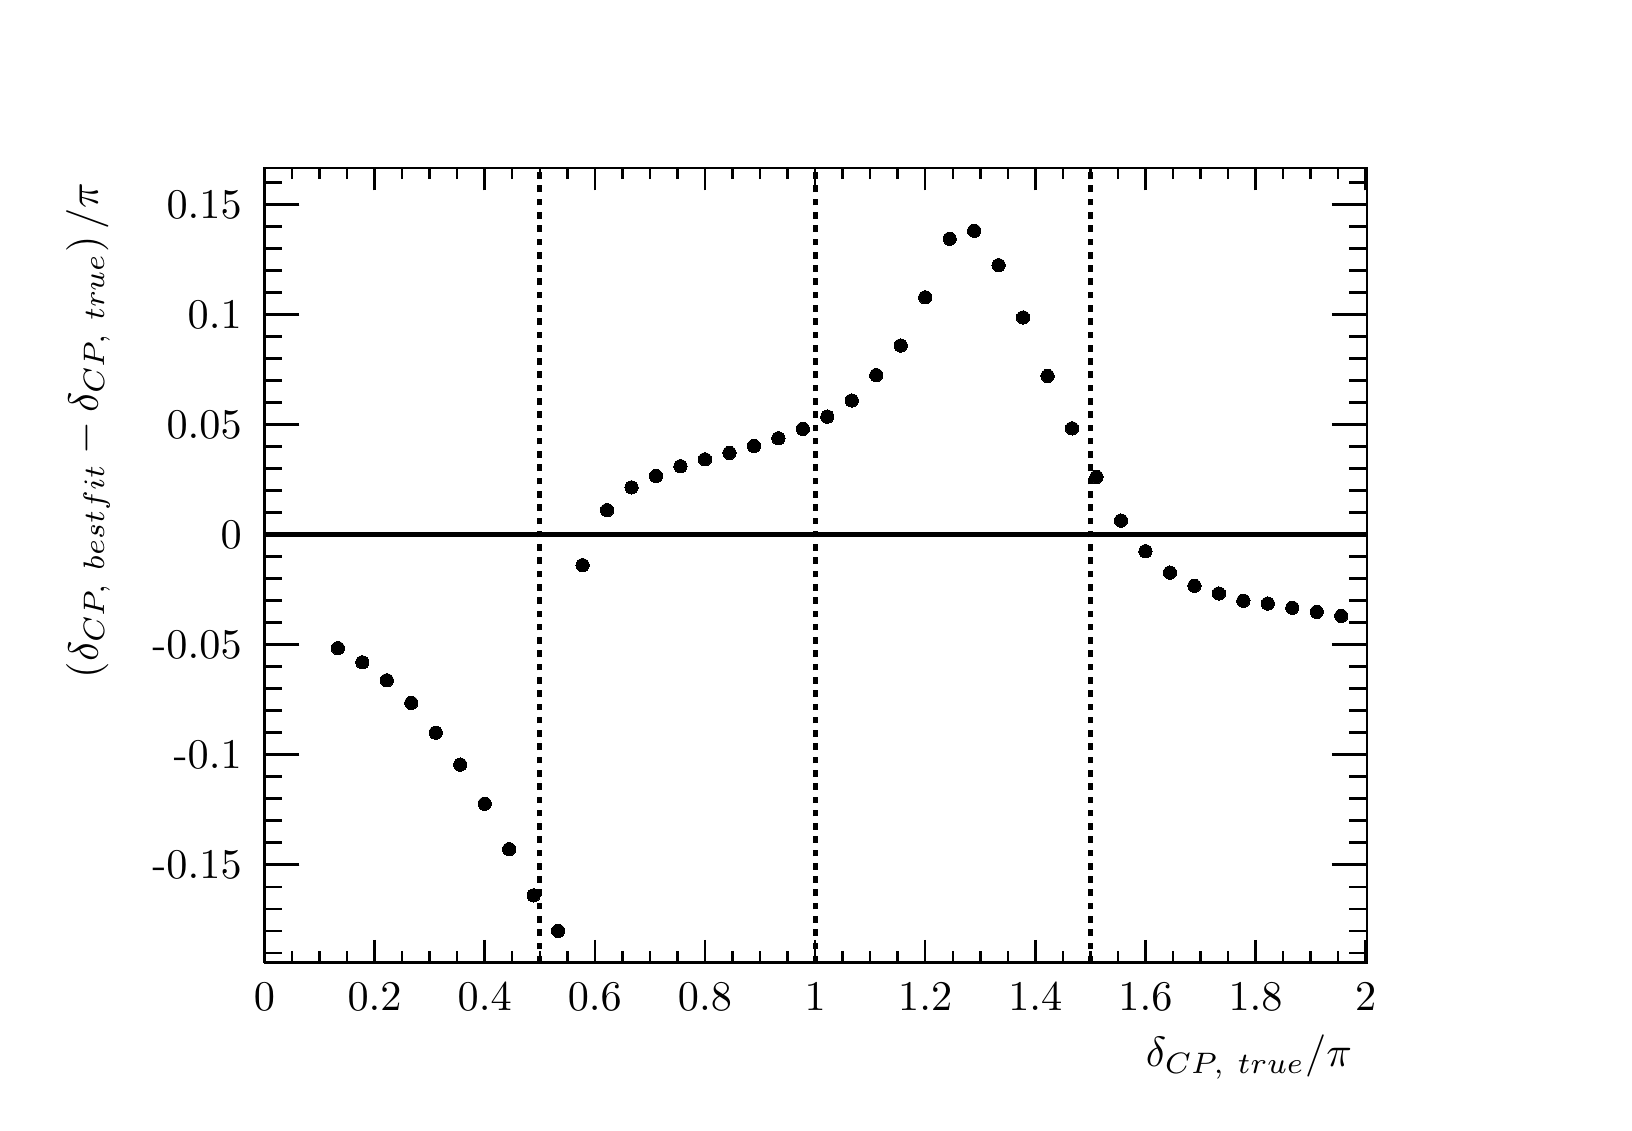
\begin{tikzpicture}
\pgfdeclareplotmark{cross} {
\pgfpathmoveto{\pgfpoint{-0.3\pgfplotmarksize}{\pgfplotmarksize}}
\pgfpathlineto{\pgfpoint{+0.3\pgfplotmarksize}{\pgfplotmarksize}}
\pgfpathlineto{\pgfpoint{+0.3\pgfplotmarksize}{0.3\pgfplotmarksize}}
\pgfpathlineto{\pgfpoint{+1\pgfplotmarksize}{0.3\pgfplotmarksize}}
\pgfpathlineto{\pgfpoint{+1\pgfplotmarksize}{-0.3\pgfplotmarksize}}
\pgfpathlineto{\pgfpoint{+0.3\pgfplotmarksize}{-0.3\pgfplotmarksize}}
\pgfpathlineto{\pgfpoint{+0.3\pgfplotmarksize}{-1.\pgfplotmarksize}}
\pgfpathlineto{\pgfpoint{-0.3\pgfplotmarksize}{-1.\pgfplotmarksize}}
\pgfpathlineto{\pgfpoint{-0.3\pgfplotmarksize}{-0.3\pgfplotmarksize}}
\pgfpathlineto{\pgfpoint{-1.\pgfplotmarksize}{-0.3\pgfplotmarksize}}
\pgfpathlineto{\pgfpoint{-1.\pgfplotmarksize}{0.3\pgfplotmarksize}}
\pgfpathlineto{\pgfpoint{-0.3\pgfplotmarksize}{0.3\pgfplotmarksize}}
\pgfpathclose
\pgfusepathqstroke
}
\pgfdeclareplotmark{cross*} {
\pgfpathmoveto{\pgfpoint{-0.3\pgfplotmarksize}{\pgfplotmarksize}}
\pgfpathlineto{\pgfpoint{+0.3\pgfplotmarksize}{\pgfplotmarksize}}
\pgfpathlineto{\pgfpoint{+0.3\pgfplotmarksize}{0.3\pgfplotmarksize}}
\pgfpathlineto{\pgfpoint{+1\pgfplotmarksize}{0.3\pgfplotmarksize}}
\pgfpathlineto{\pgfpoint{+1\pgfplotmarksize}{-0.3\pgfplotmarksize}}
\pgfpathlineto{\pgfpoint{+0.3\pgfplotmarksize}{-0.3\pgfplotmarksize}}
\pgfpathlineto{\pgfpoint{+0.3\pgfplotmarksize}{-1.\pgfplotmarksize}}
\pgfpathlineto{\pgfpoint{-0.3\pgfplotmarksize}{-1.\pgfplotmarksize}}
\pgfpathlineto{\pgfpoint{-0.3\pgfplotmarksize}{-0.3\pgfplotmarksize}}
\pgfpathlineto{\pgfpoint{-1.\pgfplotmarksize}{-0.3\pgfplotmarksize}}
\pgfpathlineto{\pgfpoint{-1.\pgfplotmarksize}{0.3\pgfplotmarksize}}
\pgfpathlineto{\pgfpoint{-0.3\pgfplotmarksize}{0.3\pgfplotmarksize}}
\pgfpathclose
\pgfusepathqfillstroke
}
\pgfdeclareplotmark{newstar} {
\pgfpathmoveto{\pgfqpoint{0pt}{\pgfplotmarksize}}
\pgfpathlineto{\pgfqpointpolar{44}{0.5\pgfplotmarksize}}
\pgfpathlineto{\pgfqpointpolar{18}{\pgfplotmarksize}}
\pgfpathlineto{\pgfqpointpolar{-20}{0.5\pgfplotmarksize}}
\pgfpathlineto{\pgfqpointpolar{-54}{\pgfplotmarksize}}
\pgfpathlineto{\pgfqpointpolar{-90}{0.5\pgfplotmarksize}}
\pgfpathlineto{\pgfqpointpolar{234}{\pgfplotmarksize}}
\pgfpathlineto{\pgfqpointpolar{198}{0.5\pgfplotmarksize}}
\pgfpathlineto{\pgfqpointpolar{162}{\pgfplotmarksize}}
\pgfpathlineto{\pgfqpointpolar{134}{0.5\pgfplotmarksize}}
\pgfpathclose
\pgfusepathqstroke
}
\pgfdeclareplotmark{newstar*} {
\pgfpathmoveto{\pgfqpoint{0pt}{\pgfplotmarksize}}
\pgfpathlineto{\pgfqpointpolar{44}{0.5\pgfplotmarksize}}
\pgfpathlineto{\pgfqpointpolar{18}{\pgfplotmarksize}}
\pgfpathlineto{\pgfqpointpolar{-20}{0.5\pgfplotmarksize}}
\pgfpathlineto{\pgfqpointpolar{-54}{\pgfplotmarksize}}
\pgfpathlineto{\pgfqpointpolar{-90}{0.5\pgfplotmarksize}}
\pgfpathlineto{\pgfqpointpolar{234}{\pgfplotmarksize}}
\pgfpathlineto{\pgfqpointpolar{198}{0.5\pgfplotmarksize}}
\pgfpathlineto{\pgfqpointpolar{162}{\pgfplotmarksize}}
\pgfpathlineto{\pgfqpointpolar{134}{0.5\pgfplotmarksize}}
\pgfpathclose
\pgfusepathqfillstroke
}
\definecolor{c}{rgb}{1,1,1};
\draw [color=c, fill=c] (0,0) rectangle (20,13.639);
\draw [color=c, fill=c] (3,1.77307) rectangle (17,11.8659);
\definecolor{c}{rgb}{0,0,0};
\draw [c,line width=0.9] (3,1.77307) -- (3,11.8659) -- (17,11.8659) -- (17,1.77307) -- (3,1.77307);
\definecolor{c}{rgb}{1,1,1};
\draw [color=c, fill=c] (3,1.77307) rectangle (17,11.8659);
\definecolor{c}{rgb}{0,0,0};
\draw [c,line width=0.9] (3,1.77307) -- (3,11.8659) -- (17,11.8659) -- (17,1.77307) -- (3,1.77307);
\draw [c,line width=0.9] (3,1.77307) -- (17,1.77307);
\draw [c,line width=0.9] (3,2.05948) -- (3,1.77307);
\draw [c,line width=0.9] (3.34965,1.91628) -- (3.34965,1.77307);
\draw [c,line width=0.9] (3.6993,1.91628) -- (3.6993,1.77307);
\draw [c,line width=0.9] (4.04895,1.91628) -- (4.04895,1.77307);
\draw [c,line width=0.9] (4.3986,2.05948) -- (4.3986,1.77307);
\draw [c,line width=0.9] (4.74825,1.91628) -- (4.74825,1.77307);
\draw [c,line width=0.9] (5.0979,1.91628) -- (5.0979,1.77307);
\draw [c,line width=0.9] (5.44755,1.91628) -- (5.44755,1.77307);
\draw [c,line width=0.9] (5.7972,2.05948) -- (5.7972,1.77307);
\draw [c,line width=0.9] (6.14685,1.91628) -- (6.14685,1.77307);
\draw [c,line width=0.9] (6.4965,1.91628) -- (6.4965,1.77307);
\draw [c,line width=0.9] (6.84615,1.91628) -- (6.84615,1.77307);
\draw [c,line width=0.9] (7.1958,2.05948) -- (7.1958,1.77307);
\draw [c,line width=0.9] (7.54545,1.91628) -- (7.54545,1.77307);
\draw [c,line width=0.9] (7.8951,1.91628) -- (7.8951,1.77307);
\draw [c,line width=0.9] (8.24475,1.91628) -- (8.24475,1.77307);
\draw [c,line width=0.9] (8.59441,2.05948) -- (8.59441,1.77307);
\draw [c,line width=0.9] (8.94406,1.91628) -- (8.94406,1.77307);
\draw [c,line width=0.9] (9.29371,1.91628) -- (9.29371,1.77307);
\draw [c,line width=0.9] (9.64336,1.91628) -- (9.64336,1.77307);
\draw [c,line width=0.9] (9.99301,2.05948) -- (9.99301,1.77307);
\draw [c,line width=0.9] (10.3427,1.91628) -- (10.3427,1.77307);
\draw [c,line width=0.9] (10.6923,1.91628) -- (10.6923,1.77307);
\draw [c,line width=0.9] (11.042,1.91628) -- (11.042,1.77307);
\draw [c,line width=0.9] (11.3916,2.05948) -- (11.3916,1.77307);
\draw [c,line width=0.9] (11.7413,1.91628) -- (11.7413,1.77307);
\draw [c,line width=0.9] (12.0909,1.91628) -- (12.0909,1.77307);
\draw [c,line width=0.9] (12.4406,1.91628) -- (12.4406,1.77307);
\draw [c,line width=0.9] (12.7902,2.05948) -- (12.7902,1.77307);
\draw [c,line width=0.9] (13.1399,1.91628) -- (13.1399,1.77307);
\draw [c,line width=0.9] (13.4895,1.91628) -- (13.4895,1.77307);
\draw [c,line width=0.9] (13.8392,1.91628) -- (13.8392,1.77307);
\draw [c,line width=0.9] (14.1888,2.05948) -- (14.1888,1.77307);
\draw [c,line width=0.9] (14.5385,1.91628) -- (14.5385,1.77307);
\draw [c,line width=0.9] (14.8881,1.91628) -- (14.8881,1.77307);
\draw [c,line width=0.9] (15.2378,1.91628) -- (15.2378,1.77307);
\draw [c,line width=0.9] (15.5874,2.05948) -- (15.5874,1.77307);
\draw [c,line width=0.9] (15.9371,1.91628) -- (15.9371,1.77307);
\draw [c,line width=0.9] (16.2867,1.91628) -- (16.2867,1.77307);
\draw [c,line width=0.9] (16.6364,1.91628) -- (16.6364,1.77307);
\draw [c,line width=0.9] (16.986,2.05948) -- (16.986,1.77307);
\draw [c,line width=0.9] (16.986,2.05948) -- (16.986,1.77307);
\draw [anchor=base] (3,1.15931) node[scale=1.52731, color=c, rotate=0]{0};
\draw [anchor=base] (4.3986,1.15931) node[scale=1.52731, color=c, rotate=0]{0.2};
\draw [anchor=base] (5.7972,1.15931) node[scale=1.52731, color=c, rotate=0]{0.4};
\draw [anchor=base] (7.1958,1.15931) node[scale=1.52731, color=c, rotate=0]{0.6};
\draw [anchor=base] (8.59441,1.15931) node[scale=1.52731, color=c, rotate=0]{0.8};
\draw [anchor=base] (9.99301,1.15931) node[scale=1.52731, color=c, rotate=0]{1};
\draw [anchor=base] (11.3916,1.15931) node[scale=1.52731, color=c, rotate=0]{1.2};
\draw [anchor=base] (12.7902,1.15931) node[scale=1.52731, color=c, rotate=0]{1.4};
\draw [anchor=base] (14.1888,1.15931) node[scale=1.52731, color=c, rotate=0]{1.6};
\draw [anchor=base] (15.5874,1.15931) node[scale=1.52731, color=c, rotate=0]{1.8};
\draw [anchor=base] (16.986,1.15931) node[scale=1.52731, color=c, rotate=0]{2};
\draw [anchor= east] (17,0.572837) node[scale=1.52731, color=c, rotate=0]{$\delta_{CP,~\text{true}} / \pi$};
\draw [c,line width=0.9] (3,11.8659) -- (17,11.8659);
\draw [c,line width=0.9] (3,11.5795) -- (3,11.8659);
\draw [c,line width=0.9] (3.34965,11.7227) -- (3.34965,11.8659);
\draw [c,line width=0.9] (3.6993,11.7227) -- (3.6993,11.8659);
\draw [c,line width=0.9] (4.04895,11.7227) -- (4.04895,11.8659);
\draw [c,line width=0.9] (4.3986,11.5795) -- (4.3986,11.8659);
\draw [c,line width=0.9] (4.74825,11.7227) -- (4.74825,11.8659);
\draw [c,line width=0.9] (5.0979,11.7227) -- (5.0979,11.8659);
\draw [c,line width=0.9] (5.44755,11.7227) -- (5.44755,11.8659);
\draw [c,line width=0.9] (5.7972,11.5795) -- (5.7972,11.8659);
\draw [c,line width=0.9] (6.14685,11.7227) -- (6.14685,11.8659);
\draw [c,line width=0.9] (6.4965,11.7227) -- (6.4965,11.8659);
\draw [c,line width=0.9] (6.84615,11.7227) -- (6.84615,11.8659);
\draw [c,line width=0.9] (7.1958,11.5795) -- (7.1958,11.8659);
\draw [c,line width=0.9] (7.54545,11.7227) -- (7.54545,11.8659);
\draw [c,line width=0.9] (7.8951,11.7227) -- (7.8951,11.8659);
\draw [c,line width=0.9] (8.24475,11.7227) -- (8.24475,11.8659);
\draw [c,line width=0.9] (8.59441,11.5795) -- (8.59441,11.8659);
\draw [c,line width=0.9] (8.94406,11.7227) -- (8.94406,11.8659);
\draw [c,line width=0.9] (9.29371,11.7227) -- (9.29371,11.8659);
\draw [c,line width=0.9] (9.64336,11.7227) -- (9.64336,11.8659);
\draw [c,line width=0.9] (9.99301,11.5795) -- (9.99301,11.8659);
\draw [c,line width=0.9] (10.3427,11.7227) -- (10.3427,11.8659);
\draw [c,line width=0.9] (10.6923,11.7227) -- (10.6923,11.8659);
\draw [c,line width=0.9] (11.042,11.7227) -- (11.042,11.8659);
\draw [c,line width=0.9] (11.3916,11.5795) -- (11.3916,11.8659);
\draw [c,line width=0.9] (11.7413,11.7227) -- (11.7413,11.8659);
\draw [c,line width=0.9] (12.0909,11.7227) -- (12.0909,11.8659);
\draw [c,line width=0.9] (12.4406,11.7227) -- (12.4406,11.8659);
\draw [c,line width=0.9] (12.7902,11.5795) -- (12.7902,11.8659);
\draw [c,line width=0.9] (13.1399,11.7227) -- (13.1399,11.8659);
\draw [c,line width=0.9] (13.4895,11.7227) -- (13.4895,11.8659);
\draw [c,line width=0.9] (13.8392,11.7227) -- (13.8392,11.8659);
\draw [c,line width=0.9] (14.1888,11.5795) -- (14.1888,11.8659);
\draw [c,line width=0.9] (14.5385,11.7227) -- (14.5385,11.8659);
\draw [c,line width=0.9] (14.8881,11.7227) -- (14.8881,11.8659);
\draw [c,line width=0.9] (15.2378,11.7227) -- (15.2378,11.8659);
\draw [c,line width=0.9] (15.5874,11.5795) -- (15.5874,11.8659);
\draw [c,line width=0.9] (15.9371,11.7227) -- (15.9371,11.8659);
\draw [c,line width=0.9] (16.2867,11.7227) -- (16.2867,11.8659);
\draw [c,line width=0.9] (16.6364,11.7227) -- (16.6364,11.8659);
\draw [c,line width=0.9] (16.986,11.5795) -- (16.986,11.8659);
\draw [c,line width=0.9] (16.986,11.5795) -- (16.986,11.8659);
\draw [c,line width=0.9] (3,1.77307) -- (3,11.8659);
\draw [c,line width=0.9] (3.444,3.01526) -- (3,3.01526);
\draw [c,line width=0.9] (3.222,3.29475) -- (3,3.29475);
\draw [c,line width=0.9] (3.222,3.57425) -- (3,3.57425);
\draw [c,line width=0.9] (3.222,3.85374) -- (3,3.85374);
\draw [c,line width=0.9] (3.222,4.13324) -- (3,4.13324);
\draw [c,line width=0.9] (3.444,4.41273) -- (3,4.41273);
\draw [c,line width=0.9] (3.222,4.69222) -- (3,4.69222);
\draw [c,line width=0.9] (3.222,4.97172) -- (3,4.97172);
\draw [c,line width=0.9] (3.222,5.25121) -- (3,5.25121);
\draw [c,line width=0.9] (3.222,5.53071) -- (3,5.53071);
\draw [c,line width=0.9] (3.444,5.8102) -- (3,5.8102);
\draw [c,line width=0.9] (3.222,6.08969) -- (3,6.08969);
\draw [c,line width=0.9] (3.222,6.36919) -- (3,6.36919);
\draw [c,line width=0.9] (3.222,6.64868) -- (3,6.64868);
\draw [c,line width=0.9] (3.222,6.92818) -- (3,6.92818);
\draw [c,line width=0.9] (3.444,7.20767) -- (3,7.20767);
\draw [c,line width=0.9] (3.222,7.48716) -- (3,7.48716);
\draw [c,line width=0.9] (3.222,7.76666) -- (3,7.76666);
\draw [c,line width=0.9] (3.222,8.04615) -- (3,8.04615);
\draw [c,line width=0.9] (3.222,8.32565) -- (3,8.32565);
\draw [c,line width=0.9] (3.444,8.60514) -- (3,8.60514);
\draw [c,line width=0.9] (3.222,8.88463) -- (3,8.88463);
\draw [c,line width=0.9] (3.222,9.16413) -- (3,9.16413);
\draw [c,line width=0.9] (3.222,9.44362) -- (3,9.44362);
\draw [c,line width=0.9] (3.222,9.72312) -- (3,9.72312);
\draw [c,line width=0.9] (3.444,10.0026) -- (3,10.0026);
\draw [c,line width=0.9] (3.222,10.2821) -- (3,10.2821);
\draw [c,line width=0.9] (3.222,10.5616) -- (3,10.5616);
\draw [c,line width=0.9] (3.222,10.8411) -- (3,10.8411);
\draw [c,line width=0.9] (3.222,11.1206) -- (3,11.1206);
\draw [c,line width=0.9] (3.444,11.4001) -- (3,11.4001);
\draw [c,line width=0.9] (3.444,3.01526) -- (3,3.01526);
\draw [c,line width=0.9] (3.222,2.73577) -- (3,2.73577);
\draw [c,line width=0.9] (3.222,2.45627) -- (3,2.45627);
\draw [c,line width=0.9] (3.222,2.17678) -- (3,2.17678);
\draw [c,line width=0.9] (3.222,1.89729) -- (3,1.89729);
\draw [c,line width=0.9] (3.444,11.4001) -- (3,11.4001);
\draw [c,line width=0.9] (3.222,11.6796) -- (3,11.6796);
\draw [anchor= east] (2.9,3.01526) node[scale=1.52731, color=c, rotate=0]{-0.15};
\draw [anchor= east] (2.9,4.41273) node[scale=1.52731, color=c, rotate=0]{-0.1};
\draw [anchor= east] (2.9,5.8102) node[scale=1.52731, color=c, rotate=0]{-0.05};
\draw [anchor= east] (2.9,7.20767) node[scale=1.52731, color=c, rotate=0]{0};
\draw [anchor= east] (2.9,8.60514) node[scale=1.52731, color=c, rotate=0]{0.05};
\draw [anchor= east] (2.9,10.0026) node[scale=1.52731, color=c, rotate=0]{0.1};
\draw [anchor= east] (2.9,11.4001) node[scale=1.52731, color=c, rotate=0]{0.15};
\draw [anchor= east] (0.76,11.8659) node[scale=1.52731, color=c, rotate=90]{$\left( \delta_{CP,~\text{best fit}} - \delta_{CP,~\text{true}} \right) / \pi$};
\draw [c,line width=0.9] (17,1.77307) -- (17,11.8659);
\draw [c,line width=0.9] (16.556,3.01526) -- (17,3.01526);
\draw [c,line width=0.9] (16.778,3.29475) -- (17,3.29475);
\draw [c,line width=0.9] (16.778,3.57425) -- (17,3.57425);
\draw [c,line width=0.9] (16.778,3.85374) -- (17,3.85374);
\draw [c,line width=0.9] (16.778,4.13324) -- (17,4.13324);
\draw [c,line width=0.9] (16.556,4.41273) -- (17,4.41273);
\draw [c,line width=0.9] (16.778,4.69222) -- (17,4.69222);
\draw [c,line width=0.9] (16.778,4.97172) -- (17,4.97172);
\draw [c,line width=0.9] (16.778,5.25121) -- (17,5.25121);
\draw [c,line width=0.9] (16.778,5.53071) -- (17,5.53071);
\draw [c,line width=0.9] (16.556,5.8102) -- (17,5.8102);
\draw [c,line width=0.9] (16.778,6.08969) -- (17,6.08969);
\draw [c,line width=0.9] (16.778,6.36919) -- (17,6.36919);
\draw [c,line width=0.9] (16.778,6.64868) -- (17,6.64868);
\draw [c,line width=0.9] (16.778,6.92818) -- (17,6.92818);
\draw [c,line width=0.9] (16.556,7.20767) -- (17,7.20767);
\draw [c,line width=0.9] (16.778,7.48716) -- (17,7.48716);
\draw [c,line width=0.9] (16.778,7.76666) -- (17,7.76666);
\draw [c,line width=0.9] (16.778,8.04615) -- (17,8.04615);
\draw [c,line width=0.9] (16.778,8.32565) -- (17,8.32565);
\draw [c,line width=0.9] (16.556,8.60514) -- (17,8.60514);
\draw [c,line width=0.9] (16.778,8.88463) -- (17,8.88463);
\draw [c,line width=0.9] (16.778,9.16413) -- (17,9.16413);
\draw [c,line width=0.9] (16.778,9.44362) -- (17,9.44362);
\draw [c,line width=0.9] (16.778,9.72312) -- (17,9.72312);
\draw [c,line width=0.9] (16.556,10.0026) -- (17,10.0026);
\draw [c,line width=0.9] (16.778,10.2821) -- (17,10.2821);
\draw [c,line width=0.9] (16.778,10.5616) -- (17,10.5616);
\draw [c,line width=0.9] (16.778,10.8411) -- (17,10.8411);
\draw [c,line width=0.9] (16.778,11.1206) -- (17,11.1206);
\draw [c,line width=0.9] (16.556,11.4001) -- (17,11.4001);
\draw [c,line width=0.9] (16.556,3.01526) -- (17,3.01526);
\draw [c,line width=0.9] (16.778,2.73577) -- (17,2.73577);
\draw [c,line width=0.9] (16.778,2.45627) -- (17,2.45627);
\draw [c,line width=0.9] (16.778,2.17678) -- (17,2.17678);
\draw [c,line width=0.9] (16.778,1.89729) -- (17,1.89729);
\draw [c,line width=0.9] (16.556,11.4001) -- (17,11.4001);
\draw [c,line width=0.9] (16.778,11.6796) -- (17,11.6796);
\foreach \P in {(3.9324,5.76608), (4.2432,5.58593), (4.554,5.35762), (4.8648,5.07113), (5.1756,4.69224), (5.4864,4.2865), (5.7972,3.79035), (6.108,3.21289), (6.4188,2.62632), (6.7296,2.17554), (7.0404,6.81969), (7.3512,7.51835), (7.662,7.8076),
 (7.97281,7.95227), (8.28361,8.07628), (8.59441,8.16367), (8.90521,8.24539), (9.21601,8.33282), (9.52681,8.43079), (9.83761,8.55175), (10.1484,8.70606), (10.4592,8.91108), (10.77,9.23315), (11.0808,9.60927), (11.3916,10.2215), (11.7024,10.9653),
 (12.0132,11.067), (12.324,10.6293), (12.6348,9.96566), (12.9456,9.22254), (13.2564,8.55726), (13.5672,7.94024), (13.878,7.38589), (14.1888,6.9972), (14.4996,6.72496), (14.8104,6.55773), (15.1212,6.46015), (15.432,6.36803), (15.7428,6.33215),
 (16.0536,6.27896), (16.3644,6.22681), (16.6752,6.17509)}{\draw[mark options={color=c,fill=c},mark size=2.402402pt, line width=0.000000pt, mark=*] plot coordinates {\P};}
\definecolor{c}{rgb}{1,1,1};
\draw [color=c, fill=c] (2,12.8206) rectangle (18,13.5708);
\definecolor{c}{rgb}{0,0,0};
\draw [c,line width=1.8] (3,7.20767) -- (16.986,7.20767);
\draw [c,dash pattern=on 2.40pt off 2.40pt ,line width=1.8] (6.4965,1.77307) -- (6.4965,11.8659);
\draw [c,dash pattern=on 2.40pt off 2.40pt ,line width=1.8] (9.99301,1.77307) -- (9.99301,11.8659);
\draw [c,dash pattern=on 2.40pt off 2.40pt ,line width=1.8] (13.4895,1.77307) -- (13.4895,11.8659);
\end{tikzpicture}

	\end{adjustbox}
	\caption[Example of \dcp bias in FD-only fits using NuWro data]{Bias in \dcp generated in FD-only fits using NuWro as `mock data' as a function of the true value of \dcp.}
	\label{fig:dcpBiasNoWgt}
\end{figure}

Given that there is a large variation in the observed bias and the value of \dcp is not known, a useful metric to judge the level of bias by is the value for which 68\% of biases are below.
In this case, this number is \ang{16.2}.

This can be compared with the expected DUNE resolution on \dcp, shown in \citefig{fig:dcpResDUNE}. 
One can see that these biases are comparable to the eventual expected \dcp resolution of DUNE.
\begin{figure}[h]
	\centering
	\includegraphics[width=.5\linewidth]{files/figures/dune_ndrwt/dcpResWithLines-cropped}
	\caption[\dcp resolution of DUNE as a function of exposure]{\dcp resolution of DUNE as a function of exposure, from~\cite{Abi:2020qib}. Additionally, a line has been drawn indicating the maximal \dcp bias created by using this incorrect interaction model (blue). The green line indicates the 68\% limit of \dcp biases.}
	\label{fig:dcpResDUNE}
\end{figure}

This bias indicates that the neutrino interaction model does not contain the required degrees of freedom to account for this alternative model.


The rest of this section is dedicated to a discussion of how it is possible to use information from ND-GAr to reduce these out-of-model biases.
Specifically, ND-GAr measures events in 3 dimensions (a two dimensional kinematic space divided up by final state) for both the nominal MC and the `mock data' sample and develops a set of weights.
The final states used are discussed in \citesec{sec:dune_ndrwt:rwt:states} while the kinematic space used is discussed in \citesec{sec:dune_ndrwt:rwt:kinematics}.
These weights are then propagated to DUNE far detector events. 
This process is described in \citesec{sec:dune_ndrwt:rwt:fd}.

\subsection{Choice of final states}
\label{sec:dune_ndrwt:rwt:states}

The reweighting is divided up into 7 final states for both horn currents.
The chosen final states are mainly based on final state pion multiplicity since the DUNE beam will produce produce a large quantity of various multiplicities.
Additionally, \citesec{sec:dune_ndrwt:pionMulti} shows that ND-GAr has a high accuracy when identifying these final states.

The chosen final states are:
\begin{itemize}
	\item $0\pi$ with a single proton in the final state
	\item $0\pi$ with more than one proton in the final state
	\item $1\piplus$ in the final state
	\item $1\piminus$ in the final state
	\item $1\pizero$ in the final state
	\item $2\pi$ in the final state, their charge is not relevant
	\item $>2\pi$ in the final state, their charge is not relevant.
\end{itemize}

The choice is made to separate the $0\pi$ final state into two separate categories due to the different processes which contribute to these final states.
A signal proton final state is commonly produced via charged current quasi-elastic (CCQE) scattering which, for a free nucleon, can be represented by the reactions
\begin{align}
	\nul + n &\rightarrow l^{-} + p \\
	\anul + p &\rightarrow l^{+} + n \, .
\end{align}
In this case the $W$ boson is absorbed by just one nucleon.

However, in a 2p2h event the $W$ boson is absorbed by two interacting nucleons within the nucleus, potentially leading to two protons in the observed final state~\cite{2p2h}.
Because different neutrino interaction generators model these processes differently, it is decided to divide the $0\pi$ category into these two final states to try and better observe any differences.

\subsection{Choice of variables}
\label{sec:dune_ndrwt:rwt:kinematics}

Two variables are defined in which the reweighting takes place, the visible energy transfer and the visible momentum transfer. 
These variables are termed \evis and \pvis respectively.
\evis is defined as 
\begin{equation}
	\evis = T_{\textrm{p}} + E_{\pi}
\end{equation}
where $T_{\textrm{p}}$ is the total kinetic energy of any final state protons and $E_{\pi}$ is the total energy (including rest masses) of any final state pions.
One can see that any energy carried by neutrons is not measured in this definition.

\pvis is defined as
\begin{equation}
	\pvis = \sqrt{ 2(\evis + E_{\mu})(E_{\mu} - p_{\mu}\cos\theta_{\mu}) - m_{\mu}^{2} + \evis^{2} }
\end{equation}
where $E_{\mu}$ and $p_{\mu}$ are the energy and momentum of the outgoing muon.
$\theta_{\mu}$ is the angle between the outgoing muon and incoming neutrino.

Distributions of true vs. reconstructed \evis and \pvis are shown in \citefig{fig:visibleTrueReco}.
One can clearly see that in both cases, the distributions are highly diagonal.

\begin{figure}[h]
	\begin{minipage}[t]{.5\linewidth}
		\begin{adjustbox}{max totalsize=\linewidth, center}
			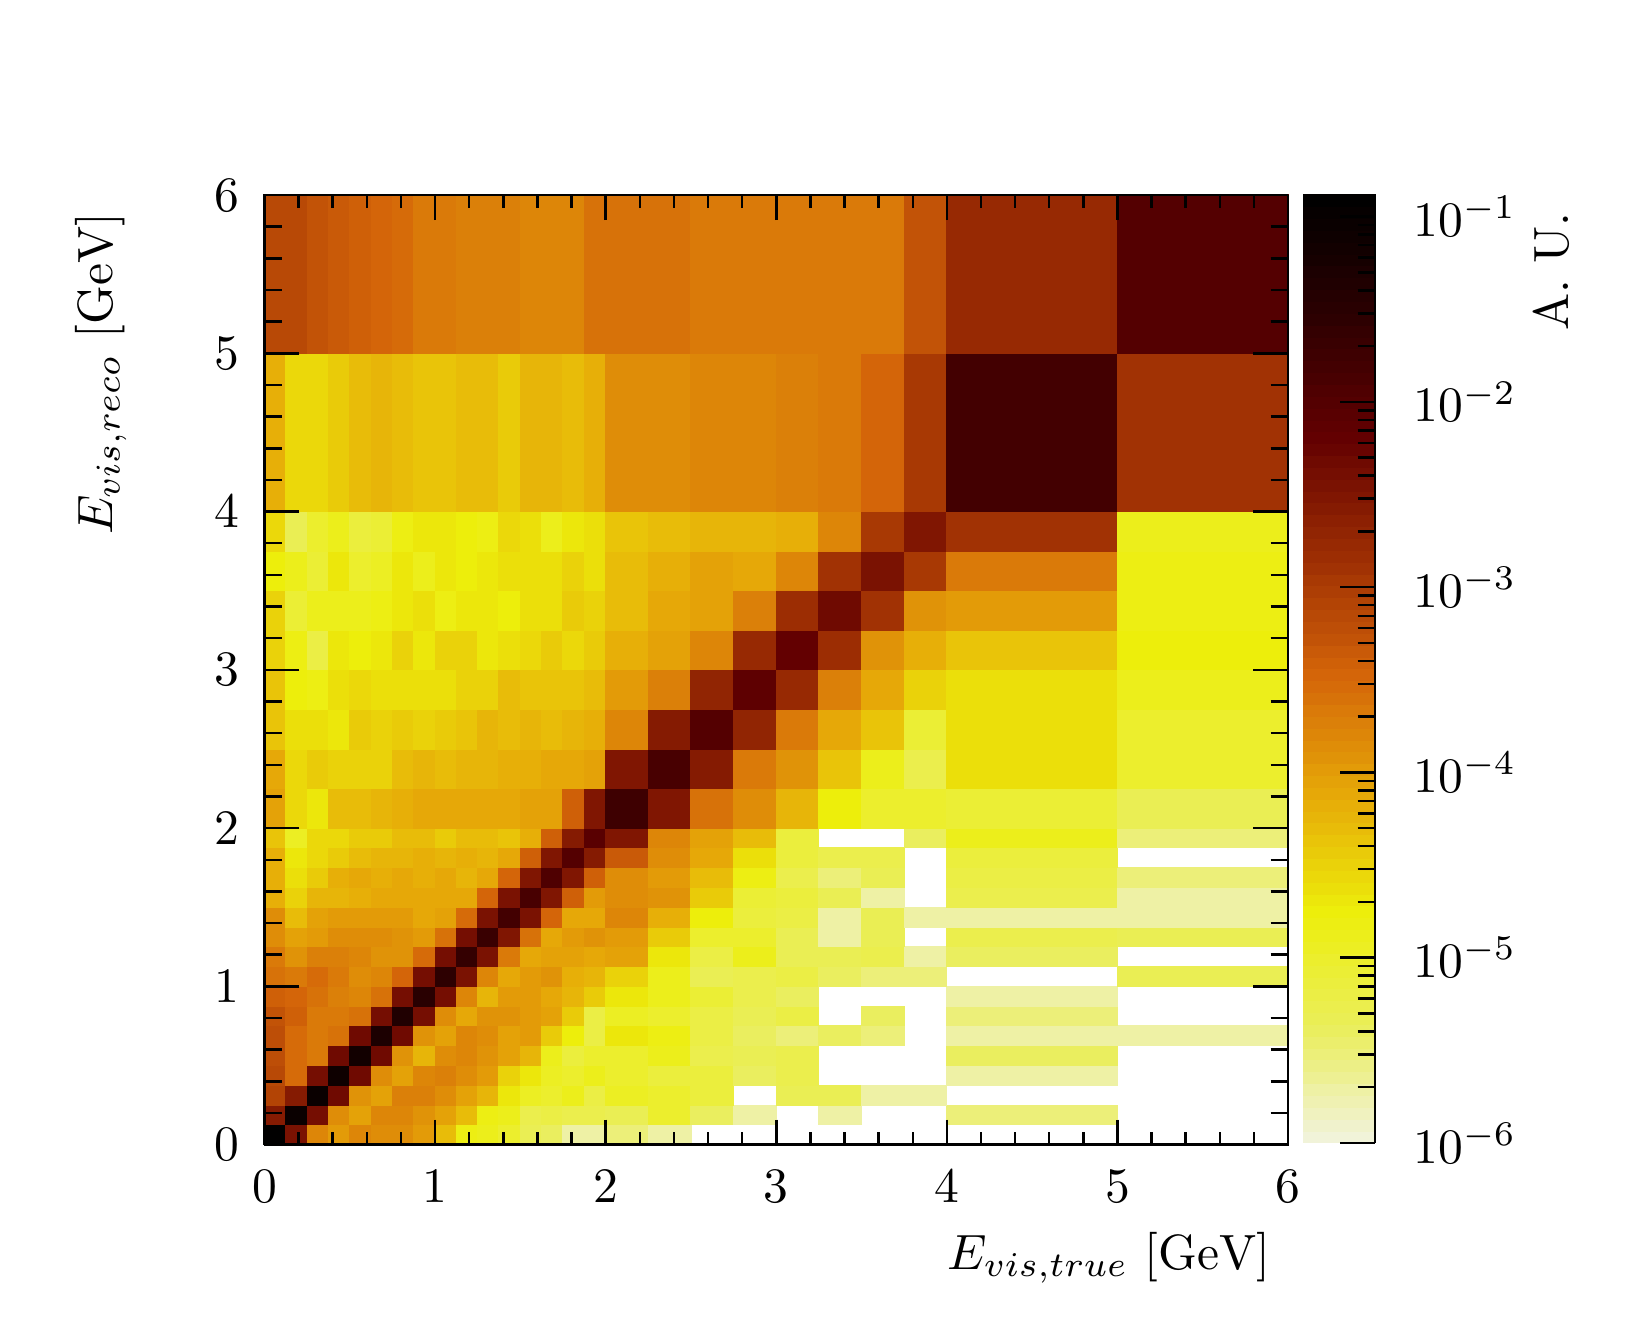
\begin{tikzpicture}
\pgfdeclareplotmark{cross} {
\pgfpathmoveto{\pgfpoint{-0.3\pgfplotmarksize}{\pgfplotmarksize}}
\pgfpathlineto{\pgfpoint{+0.3\pgfplotmarksize}{\pgfplotmarksize}}
\pgfpathlineto{\pgfpoint{+0.3\pgfplotmarksize}{0.3\pgfplotmarksize}}
\pgfpathlineto{\pgfpoint{+1\pgfplotmarksize}{0.3\pgfplotmarksize}}
\pgfpathlineto{\pgfpoint{+1\pgfplotmarksize}{-0.3\pgfplotmarksize}}
\pgfpathlineto{\pgfpoint{+0.3\pgfplotmarksize}{-0.3\pgfplotmarksize}}
\pgfpathlineto{\pgfpoint{+0.3\pgfplotmarksize}{-1.\pgfplotmarksize}}
\pgfpathlineto{\pgfpoint{-0.3\pgfplotmarksize}{-1.\pgfplotmarksize}}
\pgfpathlineto{\pgfpoint{-0.3\pgfplotmarksize}{-0.3\pgfplotmarksize}}
\pgfpathlineto{\pgfpoint{-1.\pgfplotmarksize}{-0.3\pgfplotmarksize}}
\pgfpathlineto{\pgfpoint{-1.\pgfplotmarksize}{0.3\pgfplotmarksize}}
\pgfpathlineto{\pgfpoint{-0.3\pgfplotmarksize}{0.3\pgfplotmarksize}}
\pgfpathclose
\pgfusepathqstroke
}
\pgfdeclareplotmark{cross*} {
\pgfpathmoveto{\pgfpoint{-0.3\pgfplotmarksize}{\pgfplotmarksize}}
\pgfpathlineto{\pgfpoint{+0.3\pgfplotmarksize}{\pgfplotmarksize}}
\pgfpathlineto{\pgfpoint{+0.3\pgfplotmarksize}{0.3\pgfplotmarksize}}
\pgfpathlineto{\pgfpoint{+1\pgfplotmarksize}{0.3\pgfplotmarksize}}
\pgfpathlineto{\pgfpoint{+1\pgfplotmarksize}{-0.3\pgfplotmarksize}}
\pgfpathlineto{\pgfpoint{+0.3\pgfplotmarksize}{-0.3\pgfplotmarksize}}
\pgfpathlineto{\pgfpoint{+0.3\pgfplotmarksize}{-1.\pgfplotmarksize}}
\pgfpathlineto{\pgfpoint{-0.3\pgfplotmarksize}{-1.\pgfplotmarksize}}
\pgfpathlineto{\pgfpoint{-0.3\pgfplotmarksize}{-0.3\pgfplotmarksize}}
\pgfpathlineto{\pgfpoint{-1.\pgfplotmarksize}{-0.3\pgfplotmarksize}}
\pgfpathlineto{\pgfpoint{-1.\pgfplotmarksize}{0.3\pgfplotmarksize}}
\pgfpathlineto{\pgfpoint{-0.3\pgfplotmarksize}{0.3\pgfplotmarksize}}
\pgfpathclose
\pgfusepathqfillstroke
}
\pgfdeclareplotmark{newstar} {
\pgfpathmoveto{\pgfqpoint{0pt}{\pgfplotmarksize}}
\pgfpathlineto{\pgfqpointpolar{44}{0.5\pgfplotmarksize}}
\pgfpathlineto{\pgfqpointpolar{18}{\pgfplotmarksize}}
\pgfpathlineto{\pgfqpointpolar{-20}{0.5\pgfplotmarksize}}
\pgfpathlineto{\pgfqpointpolar{-54}{\pgfplotmarksize}}
\pgfpathlineto{\pgfqpointpolar{-90}{0.5\pgfplotmarksize}}
\pgfpathlineto{\pgfqpointpolar{234}{\pgfplotmarksize}}
\pgfpathlineto{\pgfqpointpolar{198}{0.5\pgfplotmarksize}}
\pgfpathlineto{\pgfqpointpolar{162}{\pgfplotmarksize}}
\pgfpathlineto{\pgfqpointpolar{134}{0.5\pgfplotmarksize}}
\pgfpathclose
\pgfusepathqstroke
}
\pgfdeclareplotmark{newstar*} {
\pgfpathmoveto{\pgfqpoint{0pt}{\pgfplotmarksize}}
\pgfpathlineto{\pgfqpointpolar{44}{0.5\pgfplotmarksize}}
\pgfpathlineto{\pgfqpointpolar{18}{\pgfplotmarksize}}
\pgfpathlineto{\pgfqpointpolar{-20}{0.5\pgfplotmarksize}}
\pgfpathlineto{\pgfqpointpolar{-54}{\pgfplotmarksize}}
\pgfpathlineto{\pgfqpointpolar{-90}{0.5\pgfplotmarksize}}
\pgfpathlineto{\pgfqpointpolar{234}{\pgfplotmarksize}}
\pgfpathlineto{\pgfqpointpolar{198}{0.5\pgfplotmarksize}}
\pgfpathlineto{\pgfqpointpolar{162}{\pgfplotmarksize}}
\pgfpathlineto{\pgfqpointpolar{134}{0.5\pgfplotmarksize}}
\pgfpathclose
\pgfusepathqfillstroke
}
\definecolor{c}{rgb}{1,1,1};
\draw [color=c, fill=c] (0,0) rectangle (20,16.2972);
\draw [color=c, fill=c] (3,2.11864) rectangle (16,14.1786);
\definecolor{c}{rgb}{0,0,0};
\draw [c,line width=0.9] (3,2.11864) -- (3,14.1786) -- (16,14.1786) -- (16,2.11864) -- (3,2.11864);
\definecolor{c}{rgb}{1,1,1};
\draw [color=c, fill=c] (3,2.11864) rectangle (16,14.1786);
\definecolor{c}{rgb}{0,0,0};
\draw [c,line width=0.9] (3,2.11864) -- (3,14.1786) -- (16,14.1786) -- (16,2.11864) -- (3,2.11864);
\definecolor{c}{rgb}{0.00551471,0,0.000122549};
\draw [color=c, fill=c] (3,2.11864) rectangle (3.27083,2.36989);
\definecolor{c}{rgb}{0.479044,0.0716912,0.00710784};
\draw [color=c, fill=c] (3.27083,2.11864) rectangle (3.54167,2.36989);
\definecolor{c}{rgb}{0.866667,0.527451,0.0333333};
\draw [color=c, fill=c] (3.54167,2.11864) rectangle (3.8125,2.36989);
\definecolor{c}{rgb}{0.888726,0.609559,0.0321078};
\draw [color=c, fill=c] (3.8125,2.11864) rectangle (4.08333,2.36989);
\definecolor{c}{rgb}{0.866667,0.527451,0.0333333};
\draw [color=c, fill=c] (4.08333,2.11864) rectangle (4.35417,2.36989);
\definecolor{c}{rgb}{0.873284,0.552083,0.0329657};
\draw [color=c, fill=c] (4.35417,2.11864) rectangle (4.625,2.36989);
\draw [color=c, fill=c] (4.625,2.11864) rectangle (4.89583,2.36989);
\definecolor{c}{rgb}{0.888726,0.609559,0.0321078};
\draw [color=c, fill=c] (4.89583,2.11864) rectangle (5.16667,2.36989);
\definecolor{c}{rgb}{0.909681,0.736029,0.0346814};
\draw [color=c, fill=c] (5.16667,2.11864) rectangle (5.4375,2.36989);
\definecolor{c}{rgb}{0.928309,0.933333,0.0740196};
\draw [color=c, fill=c] (5.4375,2.11864) rectangle (5.70833,2.36989);
\definecolor{c}{rgb}{0.927206,0.933333,0.104902};
\draw [color=c, fill=c] (5.70833,2.11864) rectangle (5.97917,2.36989);
\definecolor{c}{rgb}{0.924632,0.933333,0.176961};
\draw [color=c, fill=c] (5.97917,2.11864) rectangle (6.25,2.36989);
\definecolor{c}{rgb}{0.919118,0.933333,0.331373};
\draw [color=c, fill=c] (6.25,2.11864) rectangle (6.52083,2.36989);
\definecolor{c}{rgb}{0.917647,0.933333,0.372549};
\draw [color=c, fill=c] (6.52083,2.11864) rectangle (6.79167,2.36989);
\definecolor{c}{rgb}{0.933839,0.943453,0.645794};
\draw [color=c, fill=c] (6.79167,2.11864) rectangle (7.0625,2.36989);
\draw [color=c, fill=c] (7.0625,2.11864) rectangle (7.33333,2.36989);
\definecolor{c}{rgb}{0.923719,0.937128,0.475016};
\draw [color=c, fill=c] (7.33333,2.11864) rectangle (7.875,2.36989);
\definecolor{c}{rgb}{0.933839,0.943453,0.645794};
\draw [color=c, fill=c] (7.875,2.11864) rectangle (8.41667,2.36989);
\definecolor{c}{rgb}{0.520956,0.104779,0.00857843};
\draw [color=c, fill=c] (3,2.36989) rectangle (3.27083,2.62114);
\definecolor{c}{rgb}{0.0386029,0,0.000857843};
\draw [color=c, fill=c] (3.27083,2.36989) rectangle (3.54167,2.62114);
\definecolor{c}{rgb}{0.458088,0.0551471,0.00637255};
\draw [color=c, fill=c] (3.54167,2.36989) rectangle (3.8125,2.62114);
\definecolor{c}{rgb}{0.873284,0.552083,0.0329657};
\draw [color=c, fill=c] (3.8125,2.36989) rectangle (4.08333,2.62114);
\definecolor{c}{rgb}{0.895343,0.634191,0.0317402};
\draw [color=c, fill=c] (4.08333,2.36989) rectangle (4.35417,2.62114);
\definecolor{c}{rgb}{0.866667,0.527451,0.0333333};
\draw [color=c, fill=c] (4.35417,2.36989) rectangle (4.625,2.62114);
\draw [color=c, fill=c] (4.625,2.36989) rectangle (4.89583,2.62114);
\definecolor{c}{rgb}{0.879902,0.576716,0.032598};
\draw [color=c, fill=c] (4.89583,2.36989) rectangle (5.16667,2.62114);
\definecolor{c}{rgb}{0.895343,0.634191,0.0317402};
\draw [color=c, fill=c] (5.16667,2.36989) rectangle (5.4375,2.62114);
\definecolor{c}{rgb}{0.909681,0.736029,0.0346814};
\draw [color=c, fill=c] (5.4375,2.36989) rectangle (5.70833,2.62114);
\definecolor{c}{rgb}{0.928309,0.933333,0.0740196};
\draw [color=c, fill=c] (5.70833,2.36989) rectangle (5.97917,2.62114);
\definecolor{c}{rgb}{0.927206,0.933333,0.104902};
\draw [color=c, fill=c] (5.97917,2.36989) rectangle (6.25,2.62114);
\definecolor{c}{rgb}{0.920221,0.933333,0.30049};
\draw [color=c, fill=c] (6.25,2.36989) rectangle (6.52083,2.62114);
\definecolor{c}{rgb}{0.921324,0.933333,0.269608};
\draw [color=c, fill=c] (6.52083,2.36989) rectangle (6.79167,2.62114);
\definecolor{c}{rgb}{0.920221,0.933333,0.30049};
\draw [color=c, fill=c] (6.79167,2.36989) rectangle (7.0625,2.62114);
\draw [color=c, fill=c] (7.0625,2.36989) rectangle (7.33333,2.62114);
\definecolor{c}{rgb}{0.919118,0.933333,0.331373};
\draw [color=c, fill=c] (7.33333,2.36989) rectangle (7.875,2.62114);
\definecolor{c}{rgb}{0.924632,0.933333,0.176961};
\draw [color=c, fill=c] (7.875,2.36989) rectangle (8.41667,2.62114);
\definecolor{c}{rgb}{0.917647,0.933333,0.372549};
\draw [color=c, fill=c] (8.41667,2.36989) rectangle (8.95833,2.62114);
\definecolor{c}{rgb}{0.933839,0.943453,0.645794};
\draw [color=c, fill=c] (8.95833,2.36989) rectangle (9.5,2.62114);
\draw [color=c, fill=c] (10.0417,2.36989) rectangle (10.5833,2.62114);
\definecolor{c}{rgb}{0.923719,0.937128,0.475016};
\draw [color=c, fill=c] (11.6667,2.36989) rectangle (13.8333,2.62114);
\definecolor{c}{rgb}{0.70098,0.265686,0.0213235};
\draw [color=c, fill=c] (3,2.62114) rectangle (3.27083,2.87239);
\definecolor{c}{rgb}{0.520956,0.104779,0.00857843};
\draw [color=c, fill=c] (3.27083,2.62114) rectangle (3.54167,2.87239);
\definecolor{c}{rgb}{0.0386029,0,0.000857843};
\draw [color=c, fill=c] (3.54167,2.62114) rectangle (3.8125,2.87239);
\definecolor{c}{rgb}{0.437132,0.0386029,0.00563726};
\draw [color=c, fill=c] (3.8125,2.62114) rectangle (4.08333,2.87239);
\definecolor{c}{rgb}{0.879902,0.576716,0.032598};
\draw [color=c, fill=c] (4.08333,2.62114) rectangle (4.35417,2.87239);
\definecolor{c}{rgb}{0.895343,0.634191,0.0317402};
\draw [color=c, fill=c] (4.35417,2.62114) rectangle (4.625,2.87239);
\definecolor{c}{rgb}{0.860049,0.502819,0.033701};
\draw [color=c, fill=c] (4.625,2.62114) rectangle (4.89583,2.87239);
\draw [color=c, fill=c] (4.89583,2.62114) rectangle (5.16667,2.87239);
\definecolor{c}{rgb}{0.873284,0.552083,0.0329657};
\draw [color=c, fill=c] (5.16667,2.62114) rectangle (5.4375,2.87239);
\definecolor{c}{rgb}{0.895343,0.634191,0.0317402};
\draw [color=c, fill=c] (5.4375,2.62114) rectangle (5.70833,2.87239);
\definecolor{c}{rgb}{0.907108,0.710294,0.0335784};
\draw [color=c, fill=c] (5.70833,2.62114) rectangle (5.97917,2.87239);
\definecolor{c}{rgb}{0.926838,0.907598,0.0420343};
\draw [color=c, fill=c] (5.97917,2.62114) rectangle (6.25,2.87239);
\definecolor{c}{rgb}{0.926103,0.933333,0.135784};
\draw [color=c, fill=c] (6.25,2.62114) rectangle (6.52083,2.87239);
\definecolor{c}{rgb}{0.924632,0.933333,0.176961};
\draw [color=c, fill=c] (6.52083,2.62114) rectangle (6.79167,2.87239);
\definecolor{c}{rgb}{0.927206,0.933333,0.104902};
\draw [color=c, fill=c] (6.79167,2.62114) rectangle (7.0625,2.87239);
\definecolor{c}{rgb}{0.921324,0.933333,0.269608};
\draw [color=c, fill=c] (7.0625,2.62114) rectangle (7.33333,2.87239);
\definecolor{c}{rgb}{0.926103,0.933333,0.135784};
\draw [color=c, fill=c] (7.33333,2.62114) rectangle (7.875,2.87239);
\definecolor{c}{rgb}{0.924632,0.933333,0.176961};
\draw [color=c, fill=c] (7.875,2.62114) rectangle (8.41667,2.87239);
\definecolor{c}{rgb}{0.922426,0.933333,0.238725};
\draw [color=c, fill=c] (8.41667,2.62114) rectangle (8.95833,2.87239);
\definecolor{c}{rgb}{0.919118,0.933333,0.331373};
\draw [color=c, fill=c] (9.5,2.62114) rectangle (10.0417,2.87239);
\draw [color=c, fill=c] (10.0417,2.62114) rectangle (10.5833,2.87239);
\definecolor{c}{rgb}{0.933839,0.943453,0.645794};
\draw [color=c, fill=c] (10.5833,2.62114) rectangle (11.125,2.87239);
\draw [color=c, fill=c] (11.125,2.62114) rectangle (11.6667,2.87239);
\definecolor{c}{rgb}{0.721569,0.286275,0.0235294};
\draw [color=c, fill=c] (3,2.87239) rectangle (3.27083,3.12364);
\definecolor{c}{rgb}{0.83799,0.420711,0.0349265};
\draw [color=c, fill=c] (3.27083,2.87239) rectangle (3.54167,3.12364);
\definecolor{c}{rgb}{0.458088,0.0551471,0.00637255};
\draw [color=c, fill=c] (3.54167,2.87239) rectangle (3.8125,3.12364);
\definecolor{c}{rgb}{0.0551471,0,0.00122549};
\draw [color=c, fill=c] (3.8125,2.87239) rectangle (4.08333,3.12364);
\definecolor{c}{rgb}{0.437132,0.0386029,0.00563726};
\draw [color=c, fill=c] (4.08333,2.87239) rectangle (4.35417,3.12364);
\definecolor{c}{rgb}{0.873284,0.552083,0.0329657};
\draw [color=c, fill=c] (4.35417,2.87239) rectangle (4.625,3.12364);
\definecolor{c}{rgb}{0.895343,0.634191,0.0317402};
\draw [color=c, fill=c] (4.625,2.87239) rectangle (4.89583,3.12364);
\definecolor{c}{rgb}{0.866667,0.527451,0.0333333};
\draw [color=c, fill=c] (4.89583,2.87239) rectangle (5.16667,3.12364);
\definecolor{c}{rgb}{0.860049,0.502819,0.033701};
\draw [color=c, fill=c] (5.16667,2.87239) rectangle (5.4375,3.12364);
\definecolor{c}{rgb}{0.873284,0.552083,0.0329657};
\draw [color=c, fill=c] (5.4375,2.87239) rectangle (5.70833,3.12364);
\definecolor{c}{rgb}{0.888726,0.609559,0.0321078};
\draw [color=c, fill=c] (5.70833,2.87239) rectangle (5.97917,3.12364);
\definecolor{c}{rgb}{0.91826,0.821814,0.0383578};
\draw [color=c, fill=c] (5.97917,2.87239) rectangle (6.25,3.12364);
\definecolor{c}{rgb}{0.926838,0.907598,0.0420343};
\draw [color=c, fill=c] (6.25,2.87239) rectangle (6.52083,3.12364);
\definecolor{c}{rgb}{0.926103,0.933333,0.135784};
\draw [color=c, fill=c] (6.52083,2.87239) rectangle (6.79167,3.12364);
\definecolor{c}{rgb}{0.924632,0.933333,0.176961};
\draw [color=c, fill=c] (6.79167,2.87239) rectangle (7.0625,3.12364);
\definecolor{c}{rgb}{0.927206,0.933333,0.104902};
\draw [color=c, fill=c] (7.0625,2.87239) rectangle (7.33333,3.12364);
\definecolor{c}{rgb}{0.924632,0.933333,0.176961};
\draw [color=c, fill=c] (7.33333,2.87239) rectangle (7.875,3.12364);
\definecolor{c}{rgb}{0.922426,0.933333,0.238725};
\draw [color=c, fill=c] (7.875,2.87239) rectangle (8.41667,3.12364);
\draw [color=c, fill=c] (8.41667,2.87239) rectangle (8.95833,3.12364);
\definecolor{c}{rgb}{0.917647,0.933333,0.372549};
\draw [color=c, fill=c] (8.95833,2.87239) rectangle (9.5,3.12364);
\definecolor{c}{rgb}{0.920221,0.933333,0.30049};
\draw [color=c, fill=c] (9.5,2.87239) rectangle (10.0417,3.12364);
\definecolor{c}{rgb}{0.933839,0.943453,0.645794};
\draw [color=c, fill=c] (11.6667,2.87239) rectangle (13.8333,3.12364);
\definecolor{c}{rgb}{0.742157,0.306863,0.0257353};
\draw [color=c, fill=c] (3,3.12364) rectangle (3.27083,3.37488);
\definecolor{c}{rgb}{0.83799,0.420711,0.0349265};
\draw [color=c, fill=c] (3.27083,3.12364) rectangle (3.54167,3.37488);
\definecolor{c}{rgb}{0.853431,0.478186,0.0340686};
\draw [color=c, fill=c] (3.54167,3.12364) rectangle (3.8125,3.37488);
\definecolor{c}{rgb}{0.437132,0.0386029,0.00563726};
\draw [color=c, fill=c] (3.8125,3.12364) rectangle (4.08333,3.37488);
\definecolor{c}{rgb}{0.0716912,0,0.00159314};
\draw [color=c, fill=c] (4.08333,3.12364) rectangle (4.35417,3.37488);
\definecolor{c}{rgb}{0.437132,0.0386029,0.00563726};
\draw [color=c, fill=c] (4.35417,3.12364) rectangle (4.625,3.37488);
\definecolor{c}{rgb}{0.879902,0.576716,0.032598};
\draw [color=c, fill=c] (4.625,3.12364) rectangle (4.89583,3.37488);
\definecolor{c}{rgb}{0.907108,0.710294,0.0335784};
\draw [color=c, fill=c] (4.89583,3.12364) rectangle (5.16667,3.37488);
\definecolor{c}{rgb}{0.873284,0.552083,0.0329657};
\draw [color=c, fill=c] (5.16667,3.12364) rectangle (5.4375,3.37488);
\definecolor{c}{rgb}{0.866667,0.527451,0.0333333};
\draw [color=c, fill=c] (5.4375,3.12364) rectangle (5.70833,3.37488);
\definecolor{c}{rgb}{0.879902,0.576716,0.032598};
\draw [color=c, fill=c] (5.70833,3.12364) rectangle (5.97917,3.37488);
\definecolor{c}{rgb}{0.895343,0.634191,0.0317402};
\draw [color=c, fill=c] (5.97917,3.12364) rectangle (6.25,3.37488);
\definecolor{c}{rgb}{0.907108,0.710294,0.0335784};
\draw [color=c, fill=c] (6.25,3.12364) rectangle (6.52083,3.37488);
\definecolor{c}{rgb}{0.927206,0.933333,0.104902};
\draw [color=c, fill=c] (6.52083,3.12364) rectangle (6.79167,3.37488);
\definecolor{c}{rgb}{0.922426,0.933333,0.238725};
\draw [color=c, fill=c] (6.79167,3.12364) rectangle (7.0625,3.37488);
\definecolor{c}{rgb}{0.924632,0.933333,0.176961};
\draw [color=c, fill=c] (7.0625,3.12364) rectangle (7.33333,3.37488);
\draw [color=c, fill=c] (7.33333,3.12364) rectangle (7.875,3.37488);
\definecolor{c}{rgb}{0.927206,0.933333,0.104902};
\draw [color=c, fill=c] (7.875,3.12364) rectangle (8.41667,3.37488);
\definecolor{c}{rgb}{0.920221,0.933333,0.30049};
\draw [color=c, fill=c] (8.41667,3.12364) rectangle (8.95833,3.37488);
\definecolor{c}{rgb}{0.919118,0.933333,0.331373};
\draw [color=c, fill=c] (8.95833,3.12364) rectangle (9.5,3.37488);
\definecolor{c}{rgb}{0.920221,0.933333,0.30049};
\draw [color=c, fill=c] (9.5,3.12364) rectangle (10.0417,3.37488);
\definecolor{c}{rgb}{0.917647,0.933333,0.372549};
\draw [color=c, fill=c] (11.6667,3.12364) rectangle (13.8333,3.37488);
\definecolor{c}{rgb}{0.742157,0.306863,0.0257353};
\draw [color=c, fill=c] (3,3.37488) rectangle (3.27083,3.62613);
\definecolor{c}{rgb}{0.83799,0.420711,0.0349265};
\draw [color=c, fill=c] (3.27083,3.37488) rectangle (3.54167,3.62613);
\definecolor{c}{rgb}{0.853431,0.478186,0.0340686};
\draw [color=c, fill=c] (3.54167,3.37488) rectangle (3.8125,3.62613);
\definecolor{c}{rgb}{0.844608,0.445343,0.0345588};
\draw [color=c, fill=c] (3.8125,3.37488) rectangle (4.08333,3.62613);
\definecolor{c}{rgb}{0.437132,0.0386029,0.00563726};
\draw [color=c, fill=c] (4.08333,3.37488) rectangle (4.35417,3.62613);
\definecolor{c}{rgb}{0.110294,0,0.00245098};
\draw [color=c, fill=c] (4.35417,3.37488) rectangle (4.625,3.62613);
\definecolor{c}{rgb}{0.437132,0.0386029,0.00563726};
\draw [color=c, fill=c] (4.625,3.37488) rectangle (4.89583,3.62613);
\definecolor{c}{rgb}{0.879902,0.576716,0.032598};
\draw [color=c, fill=c] (4.89583,3.37488) rectangle (5.16667,3.62613);
\definecolor{c}{rgb}{0.895343,0.634191,0.0317402};
\draw [color=c, fill=c] (5.16667,3.37488) rectangle (5.4375,3.62613);
\definecolor{c}{rgb}{0.866667,0.527451,0.0333333};
\draw [color=c, fill=c] (5.4375,3.37488) rectangle (5.70833,3.62613);
\definecolor{c}{rgb}{0.873284,0.552083,0.0329657};
\draw [color=c, fill=c] (5.70833,3.37488) rectangle (5.97917,3.62613);
\definecolor{c}{rgb}{0.895343,0.634191,0.0317402};
\draw [color=c, fill=c] (5.97917,3.37488) rectangle (6.25,3.62613);
\definecolor{c}{rgb}{0.888726,0.609559,0.0321078};
\draw [color=c, fill=c] (6.25,3.37488) rectangle (6.52083,3.62613);
\definecolor{c}{rgb}{0.915686,0.796078,0.0372549};
\draw [color=c, fill=c] (6.52083,3.37488) rectangle (6.79167,3.62613);
\definecolor{c}{rgb}{0.929412,0.933333,0.0431373};
\draw [color=c, fill=c] (6.79167,3.37488) rectangle (7.0625,3.62613);
\definecolor{c}{rgb}{0.921324,0.933333,0.269608};
\draw [color=c, fill=c] (7.0625,3.37488) rectangle (7.33333,3.62613);
\definecolor{c}{rgb}{0.926838,0.907598,0.0420343};
\draw [color=c, fill=c] (7.33333,3.37488) rectangle (7.875,3.62613);
\definecolor{c}{rgb}{0.928309,0.933333,0.0740196};
\draw [color=c, fill=c] (7.875,3.37488) rectangle (8.41667,3.62613);
\definecolor{c}{rgb}{0.921324,0.933333,0.269608};
\draw [color=c, fill=c] (8.41667,3.37488) rectangle (8.95833,3.62613);
\definecolor{c}{rgb}{0.917647,0.933333,0.372549};
\draw [color=c, fill=c] (8.95833,3.37488) rectangle (9.5,3.62613);
\definecolor{c}{rgb}{0.923719,0.937128,0.475016};
\draw [color=c, fill=c] (9.5,3.37488) rectangle (10.0417,3.62613);
\definecolor{c}{rgb}{0.917647,0.933333,0.372549};
\draw [color=c, fill=c] (10.0417,3.37488) rectangle (10.5833,3.62613);
\definecolor{c}{rgb}{0.923719,0.937128,0.475016};
\draw [color=c, fill=c] (10.5833,3.37488) rectangle (11.125,3.62613);
\definecolor{c}{rgb}{0.933839,0.943453,0.645794};
\draw [color=c, fill=c] (11.6667,3.37488) rectangle (13.8333,3.62613);
\draw [color=c, fill=c] (13.8333,3.37488) rectangle (16,3.62613);
\definecolor{c}{rgb}{0.762745,0.327451,0.0279412};
\draw [color=c, fill=c] (3,3.62613) rectangle (3.27083,3.87738);
\definecolor{c}{rgb}{0.810784,0.37549,0.0330882};
\draw [color=c, fill=c] (3.27083,3.62613) rectangle (3.54167,3.87738);
\definecolor{c}{rgb}{0.853431,0.478186,0.0340686};
\draw [color=c, fill=c] (3.54167,3.62613) rectangle (3.8125,3.87738);
\draw [color=c, fill=c] (3.8125,3.62613) rectangle (4.08333,3.87738);
\definecolor{c}{rgb}{0.844608,0.445343,0.0345588};
\draw [color=c, fill=c] (4.08333,3.62613) rectangle (4.35417,3.87738);
\definecolor{c}{rgb}{0.458088,0.0551471,0.00637255};
\draw [color=c, fill=c] (4.35417,3.62613) rectangle (4.625,3.87738);
\definecolor{c}{rgb}{0.126838,0,0.00281863};
\draw [color=c, fill=c] (4.625,3.62613) rectangle (4.89583,3.87738);
\definecolor{c}{rgb}{0.458088,0.0551471,0.00637255};
\draw [color=c, fill=c] (4.89583,3.62613) rectangle (5.16667,3.87738);
\definecolor{c}{rgb}{0.873284,0.552083,0.0329657};
\draw [color=c, fill=c] (5.16667,3.62613) rectangle (5.4375,3.87738);
\definecolor{c}{rgb}{0.901961,0.658824,0.0313726};
\draw [color=c, fill=c] (5.4375,3.62613) rectangle (5.70833,3.87738);
\definecolor{c}{rgb}{0.879902,0.576716,0.032598};
\draw [color=c, fill=c] (5.70833,3.62613) rectangle (5.97917,3.87738);
\draw [color=c, fill=c] (5.97917,3.62613) rectangle (6.25,3.87738);
\definecolor{c}{rgb}{0.888726,0.609559,0.0321078};
\draw [color=c, fill=c] (6.25,3.62613) rectangle (6.52083,3.87738);
\definecolor{c}{rgb}{0.895343,0.634191,0.0317402};
\draw [color=c, fill=c] (6.52083,3.62613) rectangle (6.79167,3.87738);
\definecolor{c}{rgb}{0.915686,0.796078,0.0372549};
\draw [color=c, fill=c] (6.79167,3.62613) rectangle (7.0625,3.87738);
\definecolor{c}{rgb}{0.921324,0.933333,0.269608};
\draw [color=c, fill=c] (7.0625,3.62613) rectangle (7.33333,3.87738);
\definecolor{c}{rgb}{0.926103,0.933333,0.135784};
\draw [color=c, fill=c] (7.33333,3.62613) rectangle (7.875,3.87738);
\definecolor{c}{rgb}{0.924632,0.933333,0.176961};
\draw [color=c, fill=c] (7.875,3.62613) rectangle (8.41667,3.87738);
\definecolor{c}{rgb}{0.921324,0.933333,0.269608};
\draw [color=c, fill=c] (8.41667,3.62613) rectangle (8.95833,3.87738);
\definecolor{c}{rgb}{0.919118,0.933333,0.331373};
\draw [color=c, fill=c] (8.95833,3.62613) rectangle (9.5,3.87738);
\definecolor{c}{rgb}{0.921324,0.933333,0.269608};
\draw [color=c, fill=c] (9.5,3.62613) rectangle (10.0417,3.87738);
\definecolor{c}{rgb}{0.917647,0.933333,0.372549};
\draw [color=c, fill=c] (10.5833,3.62613) rectangle (11.125,3.87738);
\definecolor{c}{rgb}{0.923719,0.937128,0.475016};
\draw [color=c, fill=c] (11.6667,3.62613) rectangle (13.8333,3.87738);
\definecolor{c}{rgb}{0.810784,0.37549,0.0330882};
\draw [color=c, fill=c] (3,3.87738) rectangle (3.27083,4.12863);
\definecolor{c}{rgb}{0.831373,0.396078,0.0352941};
\draw [color=c, fill=c] (3.27083,3.87738) rectangle (3.54167,4.12863);
\definecolor{c}{rgb}{0.844608,0.445343,0.0345588};
\draw [color=c, fill=c] (3.54167,3.87738) rectangle (3.8125,4.12863);
\definecolor{c}{rgb}{0.860049,0.502819,0.033701};
\draw [color=c, fill=c] (3.8125,3.87738) rectangle (4.08333,4.12863);
\definecolor{c}{rgb}{0.866667,0.527451,0.0333333};
\draw [color=c, fill=c] (4.08333,3.87738) rectangle (4.35417,4.12863);
\definecolor{c}{rgb}{0.844608,0.445343,0.0345588};
\draw [color=c, fill=c] (4.35417,3.87738) rectangle (4.625,4.12863);
\definecolor{c}{rgb}{0.458088,0.0551471,0.00637255};
\draw [color=c, fill=c] (4.625,3.87738) rectangle (4.89583,4.12863);
\definecolor{c}{rgb}{0.159926,0,0.00355392};
\draw [color=c, fill=c] (4.89583,3.87738) rectangle (5.16667,4.12863);
\definecolor{c}{rgb}{0.458088,0.0551471,0.00637255};
\draw [color=c, fill=c] (5.16667,3.87738) rectangle (5.4375,4.12863);
\definecolor{c}{rgb}{0.866667,0.527451,0.0333333};
\draw [color=c, fill=c] (5.4375,3.87738) rectangle (5.70833,4.12863);
\definecolor{c}{rgb}{0.907108,0.710294,0.0335784};
\draw [color=c, fill=c] (5.70833,3.87738) rectangle (5.97917,4.12863);
\definecolor{c}{rgb}{0.888726,0.609559,0.0321078};
\draw [color=c, fill=c] (5.97917,3.87738) rectangle (6.25,4.12863);
\draw [color=c, fill=c] (6.25,3.87738) rectangle (6.52083,4.12863);
\definecolor{c}{rgb}{0.901961,0.658824,0.0313726};
\draw [color=c, fill=c] (6.52083,3.87738) rectangle (6.79167,4.12863);
\definecolor{c}{rgb}{0.907108,0.710294,0.0335784};
\draw [color=c, fill=c] (6.79167,3.87738) rectangle (7.0625,4.12863);
\definecolor{c}{rgb}{0.915686,0.796078,0.0372549};
\draw [color=c, fill=c] (7.0625,3.87738) rectangle (7.33333,4.12863);
\definecolor{c}{rgb}{0.926838,0.907598,0.0420343};
\draw [color=c, fill=c] (7.33333,3.87738) rectangle (7.875,4.12863);
\definecolor{c}{rgb}{0.927206,0.933333,0.104902};
\draw [color=c, fill=c] (7.875,3.87738) rectangle (8.41667,4.12863);
\definecolor{c}{rgb}{0.923529,0.933333,0.207843};
\draw [color=c, fill=c] (8.41667,3.87738) rectangle (8.95833,4.12863);
\definecolor{c}{rgb}{0.920221,0.933333,0.30049};
\draw [color=c, fill=c] (8.95833,3.87738) rectangle (9.5,4.12863);
\definecolor{c}{rgb}{0.917647,0.933333,0.372549};
\draw [color=c, fill=c] (9.5,3.87738) rectangle (10.0417,4.12863);
\definecolor{c}{rgb}{0.933839,0.943453,0.645794};
\draw [color=c, fill=c] (11.6667,3.87738) rectangle (13.8333,4.12863);
\definecolor{c}{rgb}{0.844608,0.445343,0.0345588};
\draw [color=c, fill=c] (3,4.12863) rectangle (3.27083,4.37988);
\definecolor{c}{rgb}{0.853431,0.478186,0.0340686};
\draw [color=c, fill=c] (3.27083,4.12863) rectangle (3.54167,4.37988);
\definecolor{c}{rgb}{0.83799,0.420711,0.0349265};
\draw [color=c, fill=c] (3.54167,4.12863) rectangle (3.8125,4.37988);
\definecolor{c}{rgb}{0.853431,0.478186,0.0340686};
\draw [color=c, fill=c] (3.8125,4.12863) rectangle (4.08333,4.37988);
\definecolor{c}{rgb}{0.873284,0.552083,0.0329657};
\draw [color=c, fill=c] (4.08333,4.12863) rectangle (4.35417,4.37988);
\definecolor{c}{rgb}{0.866667,0.527451,0.0333333};
\draw [color=c, fill=c] (4.35417,4.12863) rectangle (4.625,4.37988);
\definecolor{c}{rgb}{0.831373,0.396078,0.0352941};
\draw [color=c, fill=c] (4.625,4.12863) rectangle (4.89583,4.37988);
\definecolor{c}{rgb}{0.458088,0.0551471,0.00637255};
\draw [color=c, fill=c] (4.89583,4.12863) rectangle (5.16667,4.37988);
\definecolor{c}{rgb}{0.176471,0,0.00392157};
\draw [color=c, fill=c] (5.16667,4.12863) rectangle (5.4375,4.37988);
\definecolor{c}{rgb}{0.479044,0.0716912,0.00710784};
\draw [color=c, fill=c] (5.4375,4.12863) rectangle (5.70833,4.37988);
\definecolor{c}{rgb}{0.866667,0.527451,0.0333333};
\draw [color=c, fill=c] (5.70833,4.12863) rectangle (5.97917,4.37988);
\definecolor{c}{rgb}{0.901961,0.658824,0.0313726};
\draw [color=c, fill=c] (5.97917,4.12863) rectangle (6.25,4.37988);
\definecolor{c}{rgb}{0.888726,0.609559,0.0321078};
\draw [color=c, fill=c] (6.25,4.12863) rectangle (6.52083,4.37988);
\definecolor{c}{rgb}{0.879902,0.576716,0.032598};
\draw [color=c, fill=c] (6.52083,4.12863) rectangle (6.79167,4.37988);
\definecolor{c}{rgb}{0.904534,0.684559,0.0324755};
\draw [color=c, fill=c] (6.79167,4.12863) rectangle (7.0625,4.37988);
\definecolor{c}{rgb}{0.907108,0.710294,0.0335784};
\draw [color=c, fill=c] (7.0625,4.12863) rectangle (7.33333,4.37988);
\definecolor{c}{rgb}{0.91826,0.821814,0.0383578};
\draw [color=c, fill=c] (7.33333,4.12863) rectangle (7.875,4.37988);
\definecolor{c}{rgb}{0.927206,0.933333,0.104902};
\draw [color=c, fill=c] (7.875,4.12863) rectangle (8.41667,4.37988);
\definecolor{c}{rgb}{0.919118,0.933333,0.331373};
\draw [color=c, fill=c] (8.41667,4.12863) rectangle (8.95833,4.37988);
\definecolor{c}{rgb}{0.920221,0.933333,0.30049};
\draw [color=c, fill=c] (8.95833,4.12863) rectangle (9.5,4.37988);
\definecolor{c}{rgb}{0.921324,0.933333,0.269608};
\draw [color=c, fill=c] (9.5,4.12863) rectangle (10.0417,4.37988);
\definecolor{c}{rgb}{0.917647,0.933333,0.372549};
\draw [color=c, fill=c] (10.0417,4.12863) rectangle (10.5833,4.37988);
\definecolor{c}{rgb}{0.923719,0.937128,0.475016};
\draw [color=c, fill=c] (10.5833,4.12863) rectangle (11.125,4.37988);
\draw [color=c, fill=c] (11.125,4.12863) rectangle (11.6667,4.37988);
\definecolor{c}{rgb}{0.919118,0.933333,0.331373};
\draw [color=c, fill=c] (13.8333,4.12863) rectangle (16,4.37988);
\definecolor{c}{rgb}{0.853431,0.478186,0.0340686};
\draw [color=c, fill=c] (3,4.37988) rectangle (3.27083,4.63113);
\definecolor{c}{rgb}{0.879902,0.576716,0.032598};
\draw [color=c, fill=c] (3.27083,4.37988) rectangle (3.54167,4.63113);
\definecolor{c}{rgb}{0.860049,0.502819,0.033701};
\draw [color=c, fill=c] (3.54167,4.37988) rectangle (3.8125,4.63113);
\draw [color=c, fill=c] (3.8125,4.37988) rectangle (4.08333,4.63113);
\definecolor{c}{rgb}{0.866667,0.527451,0.0333333};
\draw [color=c, fill=c] (4.08333,4.37988) rectangle (4.35417,4.63113);
\definecolor{c}{rgb}{0.879902,0.576716,0.032598};
\draw [color=c, fill=c] (4.35417,4.37988) rectangle (4.625,4.63113);
\draw [color=c, fill=c] (4.625,4.37988) rectangle (4.89583,4.63113);
\definecolor{c}{rgb}{0.83799,0.420711,0.0349265};
\draw [color=c, fill=c] (4.89583,4.37988) rectangle (5.16667,4.63113);
\definecolor{c}{rgb}{0.458088,0.0551471,0.00637255};
\draw [color=c, fill=c] (5.16667,4.37988) rectangle (5.4375,4.63113);
\definecolor{c}{rgb}{0.202941,0,0.00392157};
\draw [color=c, fill=c] (5.4375,4.37988) rectangle (5.70833,4.63113);
\definecolor{c}{rgb}{0.479044,0.0716912,0.00710784};
\draw [color=c, fill=c] (5.70833,4.37988) rectangle (5.97917,4.63113);
\definecolor{c}{rgb}{0.853431,0.478186,0.0340686};
\draw [color=c, fill=c] (5.97917,4.37988) rectangle (6.25,4.63113);
\definecolor{c}{rgb}{0.901961,0.658824,0.0313726};
\draw [color=c, fill=c] (6.25,4.37988) rectangle (6.52083,4.63113);
\definecolor{c}{rgb}{0.895343,0.634191,0.0317402};
\draw [color=c, fill=c] (6.52083,4.37988) rectangle (6.79167,4.63113);
\draw [color=c, fill=c] (6.79167,4.37988) rectangle (7.0625,4.63113);
\definecolor{c}{rgb}{0.901961,0.658824,0.0313726};
\draw [color=c, fill=c] (7.0625,4.37988) rectangle (7.33333,4.63113);
\definecolor{c}{rgb}{0.895343,0.634191,0.0317402};
\draw [color=c, fill=c] (7.33333,4.37988) rectangle (7.875,4.63113);
\definecolor{c}{rgb}{0.926838,0.907598,0.0420343};
\draw [color=c, fill=c] (7.875,4.37988) rectangle (8.41667,4.63113);
\definecolor{c}{rgb}{0.921324,0.933333,0.269608};
\draw [color=c, fill=c] (8.41667,4.37988) rectangle (8.95833,4.63113);
\definecolor{c}{rgb}{0.927206,0.933333,0.104902};
\draw [color=c, fill=c] (8.95833,4.37988) rectangle (9.5,4.63113);
\definecolor{c}{rgb}{0.919118,0.933333,0.331373};
\draw [color=c, fill=c] (9.5,4.37988) rectangle (10.0417,4.63113);
\draw [color=c, fill=c] (10.0417,4.37988) rectangle (10.5833,4.63113);
\definecolor{c}{rgb}{0.920221,0.933333,0.30049};
\draw [color=c, fill=c] (10.5833,4.37988) rectangle (11.125,4.63113);
\definecolor{c}{rgb}{0.933839,0.943453,0.645794};
\draw [color=c, fill=c] (11.125,4.37988) rectangle (11.6667,4.63113);
\definecolor{c}{rgb}{0.917647,0.933333,0.372549};
\draw [color=c, fill=c] (11.6667,4.37988) rectangle (13.8333,4.63113);
\definecolor{c}{rgb}{0.873284,0.552083,0.0329657};
\draw [color=c, fill=c] (3,4.63113) rectangle (3.27083,4.88238);
\definecolor{c}{rgb}{0.895343,0.634191,0.0317402};
\draw [color=c, fill=c] (3.27083,4.63113) rectangle (3.54167,4.88238);
\definecolor{c}{rgb}{0.888726,0.609559,0.0321078};
\draw [color=c, fill=c] (3.54167,4.63113) rectangle (3.8125,4.88238);
\definecolor{c}{rgb}{0.873284,0.552083,0.0329657};
\draw [color=c, fill=c] (3.8125,4.63113) rectangle (4.08333,4.88238);
\draw [color=c, fill=c] (4.08333,4.63113) rectangle (4.35417,4.88238);
\draw [color=c, fill=c] (4.35417,4.63113) rectangle (4.625,4.88238);
\definecolor{c}{rgb}{0.879902,0.576716,0.032598};
\draw [color=c, fill=c] (4.625,4.63113) rectangle (4.89583,4.88238);
\definecolor{c}{rgb}{0.888726,0.609559,0.0321078};
\draw [color=c, fill=c] (4.89583,4.63113) rectangle (5.16667,4.88238);
\definecolor{c}{rgb}{0.844608,0.445343,0.0345588};
\draw [color=c, fill=c] (5.16667,4.63113) rectangle (5.4375,4.88238);
\definecolor{c}{rgb}{0.458088,0.0551471,0.00637255};
\draw [color=c, fill=c] (5.4375,4.63113) rectangle (5.70833,4.88238);
\definecolor{c}{rgb}{0.222794,0,0.00392157};
\draw [color=c, fill=c] (5.70833,4.63113) rectangle (5.97917,4.88238);
\definecolor{c}{rgb}{0.5,0.0882353,0.00784314};
\draw [color=c, fill=c] (5.97917,4.63113) rectangle (6.25,4.88238);
\definecolor{c}{rgb}{0.844608,0.445343,0.0345588};
\draw [color=c, fill=c] (6.25,4.63113) rectangle (6.52083,4.88238);
\definecolor{c}{rgb}{0.901961,0.658824,0.0313726};
\draw [color=c, fill=c] (6.52083,4.63113) rectangle (6.79167,4.88238);
\definecolor{c}{rgb}{0.888726,0.609559,0.0321078};
\draw [color=c, fill=c] (6.79167,4.63113) rectangle (7.0625,4.88238);
\definecolor{c}{rgb}{0.879902,0.576716,0.032598};
\draw [color=c, fill=c] (7.0625,4.63113) rectangle (7.33333,4.88238);
\definecolor{c}{rgb}{0.888726,0.609559,0.0321078};
\draw [color=c, fill=c] (7.33333,4.63113) rectangle (7.875,4.88238);
\definecolor{c}{rgb}{0.915686,0.796078,0.0372549};
\draw [color=c, fill=c] (7.875,4.63113) rectangle (8.41667,4.88238);
\definecolor{c}{rgb}{0.924632,0.933333,0.176961};
\draw [color=c, fill=c] (8.41667,4.63113) rectangle (8.95833,4.88238);
\draw [color=c, fill=c] (8.95833,4.63113) rectangle (9.5,4.88238);
\definecolor{c}{rgb}{0.919118,0.933333,0.331373};
\draw [color=c, fill=c] (9.5,4.63113) rectangle (10.0417,4.88238);
\definecolor{c}{rgb}{0.933839,0.943453,0.645794};
\draw [color=c, fill=c] (10.0417,4.63113) rectangle (10.5833,4.88238);
\definecolor{c}{rgb}{0.919118,0.933333,0.331373};
\draw [color=c, fill=c] (10.5833,4.63113) rectangle (11.125,4.88238);
\definecolor{c}{rgb}{0.920221,0.933333,0.30049};
\draw [color=c, fill=c] (11.6667,4.63113) rectangle (13.8333,4.88238);
\definecolor{c}{rgb}{0.919118,0.933333,0.331373};
\draw [color=c, fill=c] (13.8333,4.63113) rectangle (16,4.88238);
\definecolor{c}{rgb}{0.873284,0.552083,0.0329657};
\draw [color=c, fill=c] (3,4.88238) rectangle (3.27083,5.13363);
\definecolor{c}{rgb}{0.909681,0.736029,0.0346814};
\draw [color=c, fill=c] (3.27083,4.88238) rectangle (3.54167,5.13363);
\definecolor{c}{rgb}{0.895343,0.634191,0.0317402};
\draw [color=c, fill=c] (3.54167,4.88238) rectangle (3.8125,5.13363);
\definecolor{c}{rgb}{0.888726,0.609559,0.0321078};
\draw [color=c, fill=c] (3.8125,4.88238) rectangle (4.08333,5.13363);
\draw [color=c, fill=c] (4.08333,4.88238) rectangle (4.35417,5.13363);
\draw [color=c, fill=c] (4.35417,4.88238) rectangle (4.625,5.13363);
\draw [color=c, fill=c] (4.625,4.88238) rectangle (4.89583,5.13363);
\definecolor{c}{rgb}{0.901961,0.658824,0.0313726};
\draw [color=c, fill=c] (4.89583,4.88238) rectangle (5.16667,5.13363);
\definecolor{c}{rgb}{0.895343,0.634191,0.0317402};
\draw [color=c, fill=c] (5.16667,4.88238) rectangle (5.4375,5.13363);
\definecolor{c}{rgb}{0.83799,0.420711,0.0349265};
\draw [color=c, fill=c] (5.4375,4.88238) rectangle (5.70833,5.13363);
\definecolor{c}{rgb}{0.479044,0.0716912,0.00710784};
\draw [color=c, fill=c] (5.70833,4.88238) rectangle (5.97917,5.13363);
\definecolor{c}{rgb}{0.2625,0,0.00392157};
\draw [color=c, fill=c] (5.97917,4.88238) rectangle (6.25,5.13363);
\definecolor{c}{rgb}{0.479044,0.0716912,0.00710784};
\draw [color=c, fill=c] (6.25,4.88238) rectangle (6.52083,5.13363);
\definecolor{c}{rgb}{0.831373,0.396078,0.0352941};
\draw [color=c, fill=c] (6.52083,4.88238) rectangle (6.79167,5.13363);
\definecolor{c}{rgb}{0.901961,0.658824,0.0313726};
\draw [color=c, fill=c] (6.79167,4.88238) rectangle (7.0625,5.13363);
\draw [color=c, fill=c] (7.0625,4.88238) rectangle (7.33333,5.13363);
\definecolor{c}{rgb}{0.866667,0.527451,0.0333333};
\draw [color=c, fill=c] (7.33333,4.88238) rectangle (7.875,5.13363);
\definecolor{c}{rgb}{0.904534,0.684559,0.0324755};
\draw [color=c, fill=c] (7.875,4.88238) rectangle (8.41667,5.13363);
\definecolor{c}{rgb}{0.929412,0.933333,0.0431373};
\draw [color=c, fill=c] (8.41667,4.88238) rectangle (8.95833,5.13363);
\definecolor{c}{rgb}{0.922426,0.933333,0.238725};
\draw [color=c, fill=c] (8.95833,4.88238) rectangle (9.5,5.13363);
\definecolor{c}{rgb}{0.921324,0.933333,0.269608};
\draw [color=c, fill=c] (9.5,4.88238) rectangle (10.0417,5.13363);
\definecolor{c}{rgb}{0.933839,0.943453,0.645794};
\draw [color=c, fill=c] (10.0417,4.88238) rectangle (10.5833,5.13363);
\definecolor{c}{rgb}{0.919118,0.933333,0.331373};
\draw [color=c, fill=c] (10.5833,4.88238) rectangle (11.125,5.13363);
\definecolor{c}{rgb}{0.933839,0.943453,0.645794};
\draw [color=c, fill=c] (11.125,4.88238) rectangle (11.6667,5.13363);
\draw [color=c, fill=c] (11.6667,4.88238) rectangle (13.8333,5.13363);
\draw [color=c, fill=c] (13.8333,4.88238) rectangle (16,5.13363);
\definecolor{c}{rgb}{0.904534,0.684559,0.0324755};
\draw [color=c, fill=c] (3,5.13363) rectangle (3.27083,5.38488);
\definecolor{c}{rgb}{0.91826,0.821814,0.0383578};
\draw [color=c, fill=c] (3.27083,5.13363) rectangle (3.54167,5.38488);
\definecolor{c}{rgb}{0.907108,0.710294,0.0335784};
\draw [color=c, fill=c] (3.54167,5.13363) rectangle (3.8125,5.38488);
\draw [color=c, fill=c] (3.8125,5.13363) rectangle (4.08333,5.38488);
\definecolor{c}{rgb}{0.904534,0.684559,0.0324755};
\draw [color=c, fill=c] (4.08333,5.13363) rectangle (4.35417,5.38488);
\definecolor{c}{rgb}{0.901961,0.658824,0.0313726};
\draw [color=c, fill=c] (4.35417,5.13363) rectangle (4.625,5.38488);
\draw [color=c, fill=c] (4.625,5.13363) rectangle (4.89583,5.38488);
\draw [color=c, fill=c] (4.89583,5.13363) rectangle (5.16667,5.38488);
\draw [color=c, fill=c] (5.16667,5.13363) rectangle (5.4375,5.38488);
\draw [color=c, fill=c] (5.4375,5.13363) rectangle (5.70833,5.38488);
\definecolor{c}{rgb}{0.831373,0.396078,0.0352941};
\draw [color=c, fill=c] (5.70833,5.13363) rectangle (5.97917,5.38488);
\definecolor{c}{rgb}{0.479044,0.0716912,0.00710784};
\draw [color=c, fill=c] (5.97917,5.13363) rectangle (6.25,5.38488);
\definecolor{c}{rgb}{0.282353,0,0.00392157};
\draw [color=c, fill=c] (6.25,5.13363) rectangle (6.52083,5.38488);
\definecolor{c}{rgb}{0.5,0.0882353,0.00784314};
\draw [color=c, fill=c] (6.52083,5.13363) rectangle (6.79167,5.38488);
\definecolor{c}{rgb}{0.810784,0.37549,0.0330882};
\draw [color=c, fill=c] (6.79167,5.13363) rectangle (7.0625,5.38488);
\definecolor{c}{rgb}{0.888726,0.609559,0.0321078};
\draw [color=c, fill=c] (7.0625,5.13363) rectangle (7.33333,5.38488);
\definecolor{c}{rgb}{0.873284,0.552083,0.0329657};
\draw [color=c, fill=c] (7.33333,5.13363) rectangle (7.875,5.38488);
\definecolor{c}{rgb}{0.879902,0.576716,0.032598};
\draw [color=c, fill=c] (7.875,5.13363) rectangle (8.41667,5.38488);
\definecolor{c}{rgb}{0.915686,0.796078,0.0372549};
\draw [color=c, fill=c] (8.41667,5.13363) rectangle (8.95833,5.38488);
\definecolor{c}{rgb}{0.923529,0.933333,0.207843};
\draw [color=c, fill=c] (8.95833,5.13363) rectangle (9.5,5.38488);
\definecolor{c}{rgb}{0.922426,0.933333,0.238725};
\draw [color=c, fill=c] (9.5,5.13363) rectangle (10.0417,5.38488);
\definecolor{c}{rgb}{0.919118,0.933333,0.331373};
\draw [color=c, fill=c] (10.0417,5.13363) rectangle (10.5833,5.38488);
\definecolor{c}{rgb}{0.933839,0.943453,0.645794};
\draw [color=c, fill=c] (10.5833,5.13363) rectangle (11.125,5.38488);
\definecolor{c}{rgb}{0.920221,0.933333,0.30049};
\draw [color=c, fill=c] (11.6667,5.13363) rectangle (13.8333,5.38488);
\definecolor{c}{rgb}{0.933839,0.943453,0.645794};
\draw [color=c, fill=c] (13.8333,5.13363) rectangle (16,5.38488);
\definecolor{c}{rgb}{0.904534,0.684559,0.0324755};
\draw [color=c, fill=c] (3,5.38488) rectangle (3.27083,5.63613);
\definecolor{c}{rgb}{0.923407,0.873284,0.0405637};
\draw [color=c, fill=c] (3.27083,5.38488) rectangle (3.54167,5.63613);
\definecolor{c}{rgb}{0.915686,0.796078,0.0372549};
\draw [color=c, fill=c] (3.54167,5.38488) rectangle (3.8125,5.63613);
\definecolor{c}{rgb}{0.904534,0.684559,0.0324755};
\draw [color=c, fill=c] (3.8125,5.38488) rectangle (4.08333,5.63613);
\definecolor{c}{rgb}{0.901961,0.658824,0.0313726};
\draw [color=c, fill=c] (4.08333,5.38488) rectangle (4.35417,5.63613);
\definecolor{c}{rgb}{0.904534,0.684559,0.0324755};
\draw [color=c, fill=c] (4.35417,5.38488) rectangle (4.625,5.63613);
\definecolor{c}{rgb}{0.901961,0.658824,0.0313726};
\draw [color=c, fill=c] (4.625,5.38488) rectangle (4.89583,5.63613);
\definecolor{c}{rgb}{0.904534,0.684559,0.0324755};
\draw [color=c, fill=c] (4.89583,5.38488) rectangle (5.16667,5.63613);
\definecolor{c}{rgb}{0.901961,0.658824,0.0313726};
\draw [color=c, fill=c] (5.16667,5.38488) rectangle (5.4375,5.63613);
\definecolor{c}{rgb}{0.907108,0.710294,0.0335784};
\draw [color=c, fill=c] (5.4375,5.38488) rectangle (5.70833,5.63613);
\definecolor{c}{rgb}{0.901961,0.658824,0.0313726};
\draw [color=c, fill=c] (5.70833,5.38488) rectangle (5.97917,5.63613);
\definecolor{c}{rgb}{0.831373,0.396078,0.0352941};
\draw [color=c, fill=c] (5.97917,5.38488) rectangle (6.25,5.63613);
\definecolor{c}{rgb}{0.5,0.0882353,0.00784314};
\draw [color=c, fill=c] (6.25,5.38488) rectangle (6.52083,5.63613);
\definecolor{c}{rgb}{0.308824,0,0.00392157};
\draw [color=c, fill=c] (6.52083,5.38488) rectangle (6.79167,5.63613);
\definecolor{c}{rgb}{0.5,0.0882353,0.00784314};
\draw [color=c, fill=c] (6.79167,5.38488) rectangle (7.0625,5.63613);
\definecolor{c}{rgb}{0.810784,0.37549,0.0330882};
\draw [color=c, fill=c] (7.0625,5.38488) rectangle (7.33333,5.63613);
\definecolor{c}{rgb}{0.873284,0.552083,0.0329657};
\draw [color=c, fill=c] (7.33333,5.38488) rectangle (7.875,5.63613);
\definecolor{c}{rgb}{0.888726,0.609559,0.0321078};
\draw [color=c, fill=c] (7.875,5.38488) rectangle (8.41667,5.63613);
\definecolor{c}{rgb}{0.909681,0.736029,0.0346814};
\draw [color=c, fill=c] (8.41667,5.38488) rectangle (8.95833,5.63613);
\definecolor{c}{rgb}{0.928309,0.933333,0.0740196};
\draw [color=c, fill=c] (8.95833,5.38488) rectangle (9.5,5.63613);
\definecolor{c}{rgb}{0.920221,0.933333,0.30049};
\draw [color=c, fill=c] (9.5,5.38488) rectangle (10.0417,5.63613);
\definecolor{c}{rgb}{0.923719,0.937128,0.475016};
\draw [color=c, fill=c] (10.0417,5.38488) rectangle (10.5833,5.63613);
\definecolor{c}{rgb}{0.919118,0.933333,0.331373};
\draw [color=c, fill=c] (10.5833,5.38488) rectangle (11.125,5.63613);
\definecolor{c}{rgb}{0.921324,0.933333,0.269608};
\draw [color=c, fill=c] (11.6667,5.38488) rectangle (13.8333,5.63613);
\definecolor{c}{rgb}{0.923719,0.937128,0.475016};
\draw [color=c, fill=c] (13.8333,5.38488) rectangle (16,5.63613);
\definecolor{c}{rgb}{0.904534,0.684559,0.0324755};
\draw [color=c, fill=c] (3,5.63613) rectangle (3.27083,5.88737);
\definecolor{c}{rgb}{0.926838,0.907598,0.0420343};
\draw [color=c, fill=c] (3.27083,5.63613) rectangle (3.54167,5.88737);
\definecolor{c}{rgb}{0.920833,0.847549,0.0394608};
\draw [color=c, fill=c] (3.54167,5.63613) rectangle (3.8125,5.88737);
\definecolor{c}{rgb}{0.915686,0.796078,0.0372549};
\draw [color=c, fill=c] (3.8125,5.63613) rectangle (4.08333,5.88737);
\definecolor{c}{rgb}{0.909681,0.736029,0.0346814};
\draw [color=c, fill=c] (4.08333,5.63613) rectangle (4.35417,5.88737);
\definecolor{c}{rgb}{0.907108,0.710294,0.0335784};
\draw [color=c, fill=c] (4.35417,5.63613) rectangle (4.625,5.88737);
\draw [color=c, fill=c] (4.625,5.63613) rectangle (4.89583,5.88737);
\definecolor{c}{rgb}{0.904534,0.684559,0.0324755};
\draw [color=c, fill=c] (4.89583,5.63613) rectangle (5.16667,5.88737);
\definecolor{c}{rgb}{0.907108,0.710294,0.0335784};
\draw [color=c, fill=c] (5.16667,5.63613) rectangle (5.4375,5.88737);
\definecolor{c}{rgb}{0.904534,0.684559,0.0324755};
\draw [color=c, fill=c] (5.4375,5.63613) rectangle (5.70833,5.88737);
\definecolor{c}{rgb}{0.907108,0.710294,0.0335784};
\draw [color=c, fill=c] (5.70833,5.63613) rectangle (5.97917,5.88737);
\definecolor{c}{rgb}{0.901961,0.658824,0.0313726};
\draw [color=c, fill=c] (5.97917,5.63613) rectangle (6.25,5.88737);
\definecolor{c}{rgb}{0.810784,0.37549,0.0330882};
\draw [color=c, fill=c] (6.25,5.63613) rectangle (6.52083,5.88737);
\definecolor{c}{rgb}{0.5,0.0882353,0.00784314};
\draw [color=c, fill=c] (6.52083,5.63613) rectangle (6.79167,5.88737);
\definecolor{c}{rgb}{0.328676,0,0.00392157};
\draw [color=c, fill=c] (6.79167,5.63613) rectangle (7.0625,5.88737);
\definecolor{c}{rgb}{0.520956,0.104779,0.00857843};
\draw [color=c, fill=c] (7.0625,5.63613) rectangle (7.33333,5.88737);
\definecolor{c}{rgb}{0.790196,0.354902,0.0308824};
\draw [color=c, fill=c] (7.33333,5.63613) rectangle (7.875,5.88737);
\definecolor{c}{rgb}{0.873284,0.552083,0.0329657};
\draw [color=c, fill=c] (7.875,5.63613) rectangle (8.41667,5.88737);
\definecolor{c}{rgb}{0.901961,0.658824,0.0313726};
\draw [color=c, fill=c] (8.41667,5.63613) rectangle (8.95833,5.88737);
\definecolor{c}{rgb}{0.923407,0.873284,0.0405637};
\draw [color=c, fill=c] (8.95833,5.63613) rectangle (9.5,5.88737);
\definecolor{c}{rgb}{0.922426,0.933333,0.238725};
\draw [color=c, fill=c] (9.5,5.63613) rectangle (10.0417,5.88737);
\definecolor{c}{rgb}{0.920221,0.933333,0.30049};
\draw [color=c, fill=c] (10.0417,5.63613) rectangle (10.5833,5.88737);
\draw [color=c, fill=c] (10.5833,5.63613) rectangle (11.125,5.88737);
\definecolor{c}{rgb}{0.922426,0.933333,0.238725};
\draw [color=c, fill=c] (11.6667,5.63613) rectangle (13.8333,5.88737);
\definecolor{c}{rgb}{0.913113,0.770343,0.036152};
\draw [color=c, fill=c] (3,5.88737) rectangle (3.27083,6.13862);
\definecolor{c}{rgb}{0.926103,0.933333,0.135784};
\draw [color=c, fill=c] (3.27083,5.88737) rectangle (3.54167,6.13862);
\definecolor{c}{rgb}{0.920833,0.847549,0.0394608};
\draw [color=c, fill=c] (3.54167,5.88737) rectangle (3.8125,6.13862);
\draw [color=c, fill=c] (3.8125,5.88737) rectangle (4.08333,6.13862);
\definecolor{c}{rgb}{0.915686,0.796078,0.0372549};
\draw [color=c, fill=c] (4.08333,5.88737) rectangle (4.35417,6.13862);
\draw [color=c, fill=c] (4.35417,5.88737) rectangle (4.625,6.13862);
\definecolor{c}{rgb}{0.909681,0.736029,0.0346814};
\draw [color=c, fill=c] (4.625,5.88737) rectangle (4.89583,6.13862);
\draw [color=c, fill=c] (4.89583,5.88737) rectangle (5.16667,6.13862);
\definecolor{c}{rgb}{0.915686,0.796078,0.0372549};
\draw [color=c, fill=c] (5.16667,5.88737) rectangle (5.4375,6.13862);
\definecolor{c}{rgb}{0.909681,0.736029,0.0346814};
\draw [color=c, fill=c] (5.4375,5.88737) rectangle (5.70833,6.13862);
\draw [color=c, fill=c] (5.70833,5.88737) rectangle (5.97917,6.13862);
\definecolor{c}{rgb}{0.913113,0.770343,0.036152};
\draw [color=c, fill=c] (5.97917,5.88737) rectangle (6.25,6.13862);
\definecolor{c}{rgb}{0.904534,0.684559,0.0324755};
\draw [color=c, fill=c] (6.25,5.88737) rectangle (6.52083,6.13862);
\definecolor{c}{rgb}{0.810784,0.37549,0.0330882};
\draw [color=c, fill=c] (6.52083,5.88737) rectangle (6.79167,6.13862);
\definecolor{c}{rgb}{0.520956,0.104779,0.00857843};
\draw [color=c, fill=c] (6.79167,5.88737) rectangle (7.0625,6.13862);
\definecolor{c}{rgb}{0.348529,0,0.00392157};
\draw [color=c, fill=c] (7.0625,5.88737) rectangle (7.33333,6.13862);
\definecolor{c}{rgb}{0.5,0.0882353,0.00784314};
\draw [color=c, fill=c] (7.33333,5.88737) rectangle (7.875,6.13862);
\definecolor{c}{rgb}{0.866667,0.527451,0.0333333};
\draw [color=c, fill=c] (7.875,5.88737) rectangle (8.41667,6.13862);
\definecolor{c}{rgb}{0.895343,0.634191,0.0317402};
\draw [color=c, fill=c] (8.41667,5.88737) rectangle (8.95833,6.13862);
\definecolor{c}{rgb}{0.909681,0.736029,0.0346814};
\draw [color=c, fill=c] (8.95833,5.88737) rectangle (9.5,6.13862);
\definecolor{c}{rgb}{0.922426,0.933333,0.238725};
\draw [color=c, fill=c] (9.5,5.88737) rectangle (10.0417,6.13862);
\definecolor{c}{rgb}{0.917647,0.933333,0.372549};
\draw [color=c, fill=c] (11.125,5.88737) rectangle (11.6667,6.13862);
\definecolor{c}{rgb}{0.927206,0.933333,0.104902};
\draw [color=c, fill=c] (11.6667,5.88737) rectangle (13.8333,6.13862);
\definecolor{c}{rgb}{0.923719,0.937128,0.475016};
\draw [color=c, fill=c] (13.8333,5.88737) rectangle (16,6.13862);
\definecolor{c}{rgb}{0.895343,0.634191,0.0317402};
\draw [color=c, fill=c] (3,6.13862) rectangle (3.27083,6.64112);
\definecolor{c}{rgb}{0.920833,0.847549,0.0394608};
\draw [color=c, fill=c] (3.27083,6.13862) rectangle (3.54167,6.64112);
\definecolor{c}{rgb}{0.926838,0.907598,0.0420343};
\draw [color=c, fill=c] (3.54167,6.13862) rectangle (3.8125,6.64112);
\definecolor{c}{rgb}{0.909681,0.736029,0.0346814};
\draw [color=c, fill=c] (3.8125,6.13862) rectangle (4.08333,6.64112);
\draw [color=c, fill=c] (4.08333,6.13862) rectangle (4.35417,6.64112);
\definecolor{c}{rgb}{0.907108,0.710294,0.0335784};
\draw [color=c, fill=c] (4.35417,6.13862) rectangle (4.625,6.64112);
\definecolor{c}{rgb}{0.904534,0.684559,0.0324755};
\draw [color=c, fill=c] (4.625,6.13862) rectangle (4.89583,6.64112);
\definecolor{c}{rgb}{0.901961,0.658824,0.0313726};
\draw [color=c, fill=c] (4.89583,6.13862) rectangle (5.16667,6.64112);
\draw [color=c, fill=c] (5.16667,6.13862) rectangle (5.4375,6.64112);
\draw [color=c, fill=c] (5.4375,6.13862) rectangle (5.70833,6.64112);
\draw [color=c, fill=c] (5.70833,6.13862) rectangle (5.97917,6.64112);
\draw [color=c, fill=c] (5.97917,6.13862) rectangle (6.25,6.64112);
\definecolor{c}{rgb}{0.895343,0.634191,0.0317402};
\draw [color=c, fill=c] (6.25,6.13862) rectangle (6.52083,6.64112);
\draw [color=c, fill=c] (6.52083,6.13862) rectangle (6.79167,6.64112);
\definecolor{c}{rgb}{0.810784,0.37549,0.0330882};
\draw [color=c, fill=c] (6.79167,6.13862) rectangle (7.0625,6.64112);
\definecolor{c}{rgb}{0.5,0.0882353,0.00784314};
\draw [color=c, fill=c] (7.0625,6.13862) rectangle (7.33333,6.64112);
\definecolor{c}{rgb}{0.242647,0,0.00392157};
\draw [color=c, fill=c] (7.33333,6.13862) rectangle (7.875,6.64112);
\definecolor{c}{rgb}{0.5,0.0882353,0.00784314};
\draw [color=c, fill=c] (7.875,6.13862) rectangle (8.41667,6.64112);
\definecolor{c}{rgb}{0.844608,0.445343,0.0345588};
\draw [color=c, fill=c] (8.41667,6.13862) rectangle (8.95833,6.64112);
\definecolor{c}{rgb}{0.873284,0.552083,0.0329657};
\draw [color=c, fill=c] (8.95833,6.13862) rectangle (9.5,6.64112);
\definecolor{c}{rgb}{0.907108,0.710294,0.0335784};
\draw [color=c, fill=c] (9.5,6.13862) rectangle (10.0417,6.64112);
\definecolor{c}{rgb}{0.929412,0.933333,0.0431373};
\draw [color=c, fill=c] (10.0417,6.13862) rectangle (10.5833,6.64112);
\definecolor{c}{rgb}{0.924632,0.933333,0.176961};
\draw [color=c, fill=c] (10.5833,6.13862) rectangle (11.125,6.64112);
\draw [color=c, fill=c] (11.125,6.13862) rectangle (11.6667,6.64112);
\definecolor{c}{rgb}{0.923529,0.933333,0.207843};
\draw [color=c, fill=c] (11.6667,6.13862) rectangle (13.8333,6.64112);
\definecolor{c}{rgb}{0.919118,0.933333,0.331373};
\draw [color=c, fill=c] (13.8333,6.13862) rectangle (16,6.64112);
\definecolor{c}{rgb}{0.901961,0.658824,0.0313726};
\draw [color=c, fill=c] (3,6.64112) rectangle (3.27083,7.14362);
\definecolor{c}{rgb}{0.920833,0.847549,0.0394608};
\draw [color=c, fill=c] (3.27083,6.64112) rectangle (3.54167,7.14362);
\definecolor{c}{rgb}{0.915686,0.796078,0.0372549};
\draw [color=c, fill=c] (3.54167,6.64112) rectangle (3.8125,7.14362);
\definecolor{c}{rgb}{0.91826,0.821814,0.0383578};
\draw [color=c, fill=c] (3.8125,6.64112) rectangle (4.08333,7.14362);
\draw [color=c, fill=c] (4.08333,6.64112) rectangle (4.35417,7.14362);
\draw [color=c, fill=c] (4.35417,6.64112) rectangle (4.625,7.14362);
\definecolor{c}{rgb}{0.909681,0.736029,0.0346814};
\draw [color=c, fill=c] (4.625,6.64112) rectangle (4.89583,7.14362);
\definecolor{c}{rgb}{0.907108,0.710294,0.0335784};
\draw [color=c, fill=c] (4.89583,6.64112) rectangle (5.16667,7.14362);
\definecolor{c}{rgb}{0.909681,0.736029,0.0346814};
\draw [color=c, fill=c] (5.16667,6.64112) rectangle (5.4375,7.14362);
\definecolor{c}{rgb}{0.907108,0.710294,0.0335784};
\draw [color=c, fill=c] (5.4375,6.64112) rectangle (5.70833,7.14362);
\draw [color=c, fill=c] (5.70833,6.64112) rectangle (5.97917,7.14362);
\definecolor{c}{rgb}{0.904534,0.684559,0.0324755};
\draw [color=c, fill=c] (5.97917,6.64112) rectangle (6.25,7.14362);
\draw [color=c, fill=c] (6.25,6.64112) rectangle (6.52083,7.14362);
\definecolor{c}{rgb}{0.901961,0.658824,0.0313726};
\draw [color=c, fill=c] (6.52083,6.64112) rectangle (6.79167,7.14362);
\draw [color=c, fill=c] (6.79167,6.64112) rectangle (7.0625,7.14362);
\definecolor{c}{rgb}{0.895343,0.634191,0.0317402};
\draw [color=c, fill=c] (7.0625,6.64112) rectangle (7.33333,7.14362);
\definecolor{c}{rgb}{0.5,0.0882353,0.00784314};
\draw [color=c, fill=c] (7.33333,6.64112) rectangle (7.875,7.14362);
\definecolor{c}{rgb}{0.282353,0,0.00392157};
\draw [color=c, fill=c] (7.875,6.64112) rectangle (8.41667,7.14362);
\definecolor{c}{rgb}{0.520956,0.104779,0.00857843};
\draw [color=c, fill=c] (8.41667,6.64112) rectangle (8.95833,7.14362);
\definecolor{c}{rgb}{0.853431,0.478186,0.0340686};
\draw [color=c, fill=c] (8.95833,6.64112) rectangle (9.5,7.14362);
\definecolor{c}{rgb}{0.879902,0.576716,0.032598};
\draw [color=c, fill=c] (9.5,6.64112) rectangle (10.0417,7.14362);
\definecolor{c}{rgb}{0.913113,0.770343,0.036152};
\draw [color=c, fill=c] (10.0417,6.64112) rectangle (10.5833,7.14362);
\definecolor{c}{rgb}{0.927206,0.933333,0.104902};
\draw [color=c, fill=c] (10.5833,6.64112) rectangle (11.125,7.14362);
\definecolor{c}{rgb}{0.920221,0.933333,0.30049};
\draw [color=c, fill=c] (11.125,6.64112) rectangle (11.6667,7.14362);
\definecolor{c}{rgb}{0.923407,0.873284,0.0405637};
\draw [color=c, fill=c] (11.6667,6.64112) rectangle (13.8333,7.14362);
\definecolor{c}{rgb}{0.924632,0.933333,0.176961};
\draw [color=c, fill=c] (13.8333,6.64112) rectangle (16,7.14362);
\definecolor{c}{rgb}{0.913113,0.770343,0.036152};
\draw [color=c, fill=c] (3,7.14362) rectangle (3.27083,7.64612);
\definecolor{c}{rgb}{0.923407,0.873284,0.0405637};
\draw [color=c, fill=c] (3.27083,7.14362) rectangle (3.54167,7.64612);
\draw [color=c, fill=c] (3.54167,7.14362) rectangle (3.8125,7.64612);
\definecolor{c}{rgb}{0.926838,0.907598,0.0420343};
\draw [color=c, fill=c] (3.8125,7.14362) rectangle (4.08333,7.64612);
\definecolor{c}{rgb}{0.915686,0.796078,0.0372549};
\draw [color=c, fill=c] (4.08333,7.14362) rectangle (4.35417,7.64612);
\definecolor{c}{rgb}{0.91826,0.821814,0.0383578};
\draw [color=c, fill=c] (4.35417,7.14362) rectangle (4.625,7.64612);
\definecolor{c}{rgb}{0.915686,0.796078,0.0372549};
\draw [color=c, fill=c] (4.625,7.14362) rectangle (4.89583,7.64612);
\definecolor{c}{rgb}{0.91826,0.821814,0.0383578};
\draw [color=c, fill=c] (4.89583,7.14362) rectangle (5.16667,7.64612);
\definecolor{c}{rgb}{0.915686,0.796078,0.0372549};
\draw [color=c, fill=c] (5.16667,7.14362) rectangle (5.4375,7.64612);
\definecolor{c}{rgb}{0.913113,0.770343,0.036152};
\draw [color=c, fill=c] (5.4375,7.14362) rectangle (5.70833,7.64612);
\definecolor{c}{rgb}{0.907108,0.710294,0.0335784};
\draw [color=c, fill=c] (5.70833,7.14362) rectangle (5.97917,7.64612);
\definecolor{c}{rgb}{0.909681,0.736029,0.0346814};
\draw [color=c, fill=c] (5.97917,7.14362) rectangle (6.25,7.64612);
\definecolor{c}{rgb}{0.907108,0.710294,0.0335784};
\draw [color=c, fill=c] (6.25,7.14362) rectangle (6.52083,7.64612);
\definecolor{c}{rgb}{0.909681,0.736029,0.0346814};
\draw [color=c, fill=c] (6.52083,7.14362) rectangle (6.79167,7.64612);
\definecolor{c}{rgb}{0.907108,0.710294,0.0335784};
\draw [color=c, fill=c] (6.79167,7.14362) rectangle (7.0625,7.64612);
\definecolor{c}{rgb}{0.904534,0.684559,0.0324755};
\draw [color=c, fill=c] (7.0625,7.14362) rectangle (7.33333,7.64612);
\definecolor{c}{rgb}{0.866667,0.527451,0.0333333};
\draw [color=c, fill=c] (7.33333,7.14362) rectangle (7.875,7.64612);
\definecolor{c}{rgb}{0.520956,0.104779,0.00857843};
\draw [color=c, fill=c] (7.875,7.14362) rectangle (8.41667,7.64612);
\definecolor{c}{rgb}{0.328676,0,0.00392157};
\draw [color=c, fill=c] (8.41667,7.14362) rectangle (8.95833,7.64612);
\definecolor{c}{rgb}{0.569853,0.143382,0.0102941};
\draw [color=c, fill=c] (8.95833,7.14362) rectangle (9.5,7.64612);
\definecolor{c}{rgb}{0.853431,0.478186,0.0340686};
\draw [color=c, fill=c] (9.5,7.14362) rectangle (10.0417,7.64612);
\definecolor{c}{rgb}{0.901961,0.658824,0.0313726};
\draw [color=c, fill=c] (10.0417,7.14362) rectangle (10.5833,7.64612);
\definecolor{c}{rgb}{0.913113,0.770343,0.036152};
\draw [color=c, fill=c] (10.5833,7.14362) rectangle (11.125,7.64612);
\definecolor{c}{rgb}{0.923529,0.933333,0.207843};
\draw [color=c, fill=c] (11.125,7.14362) rectangle (11.6667,7.64612);
\definecolor{c}{rgb}{0.923407,0.873284,0.0405637};
\draw [color=c, fill=c] (11.6667,7.14362) rectangle (13.8333,7.64612);
\definecolor{c}{rgb}{0.924632,0.933333,0.176961};
\draw [color=c, fill=c] (13.8333,7.14362) rectangle (16,7.64612);
\definecolor{c}{rgb}{0.913113,0.770343,0.036152};
\draw [color=c, fill=c] (3,7.64612) rectangle (3.27083,8.14861);
\definecolor{c}{rgb}{0.929412,0.933333,0.0431373};
\draw [color=c, fill=c] (3.27083,7.64612) rectangle (3.54167,8.14861);
\definecolor{c}{rgb}{0.928309,0.933333,0.0740196};
\draw [color=c, fill=c] (3.54167,7.64612) rectangle (3.8125,8.14861);
\definecolor{c}{rgb}{0.923407,0.873284,0.0405637};
\draw [color=c, fill=c] (3.8125,7.64612) rectangle (4.08333,8.14861);
\definecolor{c}{rgb}{0.920833,0.847549,0.0394608};
\draw [color=c, fill=c] (4.08333,7.64612) rectangle (4.35417,8.14861);
\definecolor{c}{rgb}{0.923407,0.873284,0.0405637};
\draw [color=c, fill=c] (4.35417,7.64612) rectangle (4.625,8.14861);
\draw [color=c, fill=c] (4.625,7.64612) rectangle (4.89583,8.14861);
\draw [color=c, fill=c] (4.89583,7.64612) rectangle (5.16667,8.14861);
\draw [color=c, fill=c] (5.16667,7.64612) rectangle (5.4375,8.14861);
\definecolor{c}{rgb}{0.91826,0.821814,0.0383578};
\draw [color=c, fill=c] (5.4375,7.64612) rectangle (5.70833,8.14861);
\draw [color=c, fill=c] (5.70833,7.64612) rectangle (5.97917,8.14861);
\definecolor{c}{rgb}{0.909681,0.736029,0.0346814};
\draw [color=c, fill=c] (5.97917,7.64612) rectangle (6.25,8.14861);
\definecolor{c}{rgb}{0.913113,0.770343,0.036152};
\draw [color=c, fill=c] (6.25,7.64612) rectangle (6.52083,8.14861);
\draw [color=c, fill=c] (6.52083,7.64612) rectangle (6.79167,8.14861);
\draw [color=c, fill=c] (6.79167,7.64612) rectangle (7.0625,8.14861);
\definecolor{c}{rgb}{0.909681,0.736029,0.0346814};
\draw [color=c, fill=c] (7.0625,7.64612) rectangle (7.33333,8.14861);
\definecolor{c}{rgb}{0.888726,0.609559,0.0321078};
\draw [color=c, fill=c] (7.33333,7.64612) rectangle (7.875,8.14861);
\definecolor{c}{rgb}{0.860049,0.502819,0.033701};
\draw [color=c, fill=c] (7.875,7.64612) rectangle (8.41667,8.14861);
\definecolor{c}{rgb}{0.569853,0.143382,0.0102941};
\draw [color=c, fill=c] (8.41667,7.64612) rectangle (8.95833,8.14861);
\definecolor{c}{rgb}{0.368382,0,0.00392157};
\draw [color=c, fill=c] (8.95833,7.64612) rectangle (9.5,8.14861);
\definecolor{c}{rgb}{0.590809,0.159926,0.0110294};
\draw [color=c, fill=c] (9.5,7.64612) rectangle (10.0417,8.14861);
\definecolor{c}{rgb}{0.860049,0.502819,0.033701};
\draw [color=c, fill=c] (10.0417,7.64612) rectangle (10.5833,8.14861);
\definecolor{c}{rgb}{0.901961,0.658824,0.0313726};
\draw [color=c, fill=c] (10.5833,7.64612) rectangle (11.125,8.14861);
\definecolor{c}{rgb}{0.91826,0.821814,0.0383578};
\draw [color=c, fill=c] (11.125,7.64612) rectangle (11.6667,8.14861);
\definecolor{c}{rgb}{0.923407,0.873284,0.0405637};
\draw [color=c, fill=c] (11.6667,7.64612) rectangle (13.8333,8.14861);
\definecolor{c}{rgb}{0.927206,0.933333,0.104902};
\draw [color=c, fill=c] (13.8333,7.64612) rectangle (16,8.14861);
\definecolor{c}{rgb}{0.91826,0.821814,0.0383578};
\draw [color=c, fill=c] (3,8.14861) rectangle (3.27083,8.65111);
\definecolor{c}{rgb}{0.928309,0.933333,0.0740196};
\draw [color=c, fill=c] (3.27083,8.14861) rectangle (3.54167,8.65111);
\definecolor{c}{rgb}{0.921324,0.933333,0.269608};
\draw [color=c, fill=c] (3.54167,8.14861) rectangle (3.8125,8.65111);
\definecolor{c}{rgb}{0.926838,0.907598,0.0420343};
\draw [color=c, fill=c] (3.8125,8.14861) rectangle (4.08333,8.65111);
\definecolor{c}{rgb}{0.929412,0.933333,0.0431373};
\draw [color=c, fill=c] (4.08333,8.14861) rectangle (4.35417,8.65111);
\definecolor{c}{rgb}{0.926838,0.907598,0.0420343};
\draw [color=c, fill=c] (4.35417,8.14861) rectangle (4.625,8.65111);
\definecolor{c}{rgb}{0.91826,0.821814,0.0383578};
\draw [color=c, fill=c] (4.625,8.14861) rectangle (4.89583,8.65111);
\definecolor{c}{rgb}{0.926838,0.907598,0.0420343};
\draw [color=c, fill=c] (4.89583,8.14861) rectangle (5.16667,8.65111);
\definecolor{c}{rgb}{0.91826,0.821814,0.0383578};
\draw [color=c, fill=c] (5.16667,8.14861) rectangle (5.4375,8.65111);
\draw [color=c, fill=c] (5.4375,8.14861) rectangle (5.70833,8.65111);
\definecolor{c}{rgb}{0.926838,0.907598,0.0420343};
\draw [color=c, fill=c] (5.70833,8.14861) rectangle (5.97917,8.65111);
\definecolor{c}{rgb}{0.923407,0.873284,0.0405637};
\draw [color=c, fill=c] (5.97917,8.14861) rectangle (6.25,8.65111);
\definecolor{c}{rgb}{0.920833,0.847549,0.0394608};
\draw [color=c, fill=c] (6.25,8.14861) rectangle (6.52083,8.65111);
\definecolor{c}{rgb}{0.915686,0.796078,0.0372549};
\draw [color=c, fill=c] (6.52083,8.14861) rectangle (6.79167,8.65111);
\definecolor{c}{rgb}{0.920833,0.847549,0.0394608};
\draw [color=c, fill=c] (6.79167,8.14861) rectangle (7.0625,8.65111);
\definecolor{c}{rgb}{0.915686,0.796078,0.0372549};
\draw [color=c, fill=c] (7.0625,8.14861) rectangle (7.33333,8.65111);
\definecolor{c}{rgb}{0.904534,0.684559,0.0324755};
\draw [color=c, fill=c] (7.33333,8.14861) rectangle (7.875,8.65111);
\definecolor{c}{rgb}{0.895343,0.634191,0.0317402};
\draw [color=c, fill=c] (7.875,8.14861) rectangle (8.41667,8.65111);
\definecolor{c}{rgb}{0.866667,0.527451,0.0333333};
\draw [color=c, fill=c] (8.41667,8.14861) rectangle (8.95833,8.65111);
\definecolor{c}{rgb}{0.590809,0.159926,0.0110294};
\draw [color=c, fill=c] (8.95833,8.14861) rectangle (9.5,8.65111);
\definecolor{c}{rgb}{0.388235,0,0.00392157};
\draw [color=c, fill=c] (9.5,8.14861) rectangle (10.0417,8.65111);
\definecolor{c}{rgb}{0.611765,0.176471,0.0117647};
\draw [color=c, fill=c] (10.0417,8.14861) rectangle (10.5833,8.65111);
\definecolor{c}{rgb}{0.879902,0.576716,0.032598};
\draw [color=c, fill=c] (10.5833,8.14861) rectangle (11.125,8.65111);
\definecolor{c}{rgb}{0.904534,0.684559,0.0324755};
\draw [color=c, fill=c] (11.125,8.14861) rectangle (11.6667,8.65111);
\definecolor{c}{rgb}{0.913113,0.770343,0.036152};
\draw [color=c, fill=c] (11.6667,8.14861) rectangle (13.8333,8.65111);
\definecolor{c}{rgb}{0.929412,0.933333,0.0431373};
\draw [color=c, fill=c] (13.8333,8.14861) rectangle (16,8.65111);
\definecolor{c}{rgb}{0.91826,0.821814,0.0383578};
\draw [color=c, fill=c] (3,8.65111) rectangle (3.27083,9.15361);
\definecolor{c}{rgb}{0.923529,0.933333,0.207843};
\draw [color=c, fill=c] (3.27083,8.65111) rectangle (3.54167,9.15361);
\definecolor{c}{rgb}{0.927206,0.933333,0.104902};
\draw [color=c, fill=c] (3.54167,8.65111) rectangle (3.8125,9.15361);
\draw [color=c, fill=c] (3.8125,8.65111) rectangle (4.08333,9.15361);
\draw [color=c, fill=c] (4.08333,8.65111) rectangle (4.35417,9.15361);
\definecolor{c}{rgb}{0.928309,0.933333,0.0740196};
\draw [color=c, fill=c] (4.35417,8.65111) rectangle (4.625,9.15361);
\definecolor{c}{rgb}{0.926838,0.907598,0.0420343};
\draw [color=c, fill=c] (4.625,8.65111) rectangle (4.89583,9.15361);
\definecolor{c}{rgb}{0.923407,0.873284,0.0405637};
\draw [color=c, fill=c] (4.89583,8.65111) rectangle (5.16667,9.15361);
\definecolor{c}{rgb}{0.928309,0.933333,0.0740196};
\draw [color=c, fill=c] (5.16667,8.65111) rectangle (5.4375,9.15361);
\definecolor{c}{rgb}{0.926838,0.907598,0.0420343};
\draw [color=c, fill=c] (5.4375,8.65111) rectangle (5.70833,9.15361);
\draw [color=c, fill=c] (5.70833,8.65111) rectangle (5.97917,9.15361);
\definecolor{c}{rgb}{0.929412,0.933333,0.0431373};
\draw [color=c, fill=c] (5.97917,8.65111) rectangle (6.25,9.15361);
\definecolor{c}{rgb}{0.923407,0.873284,0.0405637};
\draw [color=c, fill=c] (6.25,8.65111) rectangle (6.52083,9.15361);
\draw [color=c, fill=c] (6.52083,8.65111) rectangle (6.79167,9.15361);
\definecolor{c}{rgb}{0.915686,0.796078,0.0372549};
\draw [color=c, fill=c] (6.79167,8.65111) rectangle (7.0625,9.15361);
\definecolor{c}{rgb}{0.91826,0.821814,0.0383578};
\draw [color=c, fill=c] (7.0625,8.65111) rectangle (7.33333,9.15361);
\definecolor{c}{rgb}{0.909681,0.736029,0.0346814};
\draw [color=c, fill=c] (7.33333,8.65111) rectangle (7.875,9.15361);
\definecolor{c}{rgb}{0.901961,0.658824,0.0313726};
\draw [color=c, fill=c] (7.875,8.65111) rectangle (8.41667,9.15361);
\definecolor{c}{rgb}{0.895343,0.634191,0.0317402};
\draw [color=c, fill=c] (8.41667,8.65111) rectangle (8.95833,9.15361);
\definecolor{c}{rgb}{0.860049,0.502819,0.033701};
\draw [color=c, fill=c] (8.95833,8.65111) rectangle (9.5,9.15361);
\definecolor{c}{rgb}{0.611765,0.176471,0.0117647};
\draw [color=c, fill=c] (9.5,8.65111) rectangle (10.0417,9.15361);
\definecolor{c}{rgb}{0.437132,0.0386029,0.00563726};
\draw [color=c, fill=c] (10.0417,8.65111) rectangle (10.5833,9.15361);
\definecolor{c}{rgb}{0.632353,0.197059,0.0139706};
\draw [color=c, fill=c] (10.5833,8.65111) rectangle (11.125,9.15361);
\definecolor{c}{rgb}{0.879902,0.576716,0.032598};
\draw [color=c, fill=c] (11.125,8.65111) rectangle (11.6667,9.15361);
\definecolor{c}{rgb}{0.888726,0.609559,0.0321078};
\draw [color=c, fill=c] (11.6667,8.65111) rectangle (13.8333,9.15361);
\definecolor{c}{rgb}{0.928309,0.933333,0.0740196};
\draw [color=c, fill=c] (13.8333,8.65111) rectangle (16,9.15361);
\definecolor{c}{rgb}{0.929412,0.933333,0.0431373};
\draw [color=c, fill=c] (3,9.15361) rectangle (3.27083,9.65611);
\definecolor{c}{rgb}{0.927206,0.933333,0.104902};
\draw [color=c, fill=c] (3.27083,9.15361) rectangle (3.54167,9.65611);
\definecolor{c}{rgb}{0.923529,0.933333,0.207843};
\draw [color=c, fill=c] (3.54167,9.15361) rectangle (3.8125,9.65611);
\definecolor{c}{rgb}{0.926838,0.907598,0.0420343};
\draw [color=c, fill=c] (3.8125,9.15361) rectangle (4.08333,9.65611);
\definecolor{c}{rgb}{0.924632,0.933333,0.176961};
\draw [color=c, fill=c] (4.08333,9.15361) rectangle (4.35417,9.65611);
\definecolor{c}{rgb}{0.926103,0.933333,0.135784};
\draw [color=c, fill=c] (4.35417,9.15361) rectangle (4.625,9.65611);
\definecolor{c}{rgb}{0.926838,0.907598,0.0420343};
\draw [color=c, fill=c] (4.625,9.15361) rectangle (4.89583,9.65611);
\definecolor{c}{rgb}{0.927206,0.933333,0.104902};
\draw [color=c, fill=c] (4.89583,9.15361) rectangle (5.16667,9.65611);
\definecolor{c}{rgb}{0.926838,0.907598,0.0420343};
\draw [color=c, fill=c] (5.16667,9.15361) rectangle (5.4375,9.65611);
\definecolor{c}{rgb}{0.929412,0.933333,0.0431373};
\draw [color=c, fill=c] (5.4375,9.15361) rectangle (5.70833,9.65611);
\definecolor{c}{rgb}{0.926838,0.907598,0.0420343};
\draw [color=c, fill=c] (5.70833,9.15361) rectangle (5.97917,9.65611);
\definecolor{c}{rgb}{0.923407,0.873284,0.0405637};
\draw [color=c, fill=c] (5.97917,9.15361) rectangle (6.25,9.65611);
\draw [color=c, fill=c] (6.25,9.15361) rectangle (6.52083,9.65611);
\draw [color=c, fill=c] (6.52083,9.15361) rectangle (6.79167,9.65611);
\definecolor{c}{rgb}{0.91826,0.821814,0.0383578};
\draw [color=c, fill=c] (6.79167,9.15361) rectangle (7.0625,9.65611);
\definecolor{c}{rgb}{0.923407,0.873284,0.0405637};
\draw [color=c, fill=c] (7.0625,9.15361) rectangle (7.33333,9.65611);
\definecolor{c}{rgb}{0.909681,0.736029,0.0346814};
\draw [color=c, fill=c] (7.33333,9.15361) rectangle (7.875,9.65611);
\definecolor{c}{rgb}{0.904534,0.684559,0.0324755};
\draw [color=c, fill=c] (7.875,9.15361) rectangle (8.41667,9.65611);
\definecolor{c}{rgb}{0.895343,0.634191,0.0317402};
\draw [color=c, fill=c] (8.41667,9.15361) rectangle (8.95833,9.65611);
\definecolor{c}{rgb}{0.901961,0.658824,0.0313726};
\draw [color=c, fill=c] (8.95833,9.15361) rectangle (9.5,9.65611);
\definecolor{c}{rgb}{0.866667,0.527451,0.0333333};
\draw [color=c, fill=c] (9.5,9.15361) rectangle (10.0417,9.65611);
\definecolor{c}{rgb}{0.632353,0.197059,0.0139706};
\draw [color=c, fill=c] (10.0417,9.15361) rectangle (10.5833,9.65611);
\definecolor{c}{rgb}{0.479044,0.0716912,0.00710784};
\draw [color=c, fill=c] (10.5833,9.15361) rectangle (11.125,9.65611);
\definecolor{c}{rgb}{0.659804,0.22451,0.0169118};
\draw [color=c, fill=c] (11.125,9.15361) rectangle (11.6667,9.65611);
\definecolor{c}{rgb}{0.853431,0.478186,0.0340686};
\draw [color=c, fill=c] (11.6667,9.15361) rectangle (13.8333,9.65611);
\definecolor{c}{rgb}{0.928309,0.933333,0.0740196};
\draw [color=c, fill=c] (13.8333,9.15361) rectangle (16,9.65611);
\definecolor{c}{rgb}{0.920833,0.847549,0.0394608};
\draw [color=c, fill=c] (3,9.65611) rectangle (3.27083,10.1586);
\definecolor{c}{rgb}{0.919118,0.933333,0.331373};
\draw [color=c, fill=c] (3.27083,9.65611) rectangle (3.54167,10.1586);
\definecolor{c}{rgb}{0.924632,0.933333,0.176961};
\draw [color=c, fill=c] (3.54167,9.65611) rectangle (3.8125,10.1586);
\definecolor{c}{rgb}{0.927206,0.933333,0.104902};
\draw [color=c, fill=c] (3.8125,9.65611) rectangle (4.08333,10.1586);
\definecolor{c}{rgb}{0.922426,0.933333,0.238725};
\draw [color=c, fill=c] (4.08333,9.65611) rectangle (4.35417,10.1586);
\definecolor{c}{rgb}{0.923529,0.933333,0.207843};
\draw [color=c, fill=c] (4.35417,9.65611) rectangle (4.625,10.1586);
\definecolor{c}{rgb}{0.928309,0.933333,0.0740196};
\draw [color=c, fill=c] (4.625,9.65611) rectangle (4.89583,10.1586);
\definecolor{c}{rgb}{0.926838,0.907598,0.0420343};
\draw [color=c, fill=c] (4.89583,9.65611) rectangle (5.16667,10.1586);
\draw [color=c, fill=c] (5.16667,9.65611) rectangle (5.4375,10.1586);
\definecolor{c}{rgb}{0.929412,0.933333,0.0431373};
\draw [color=c, fill=c] (5.4375,9.65611) rectangle (5.70833,10.1586);
\definecolor{c}{rgb}{0.928309,0.933333,0.0740196};
\draw [color=c, fill=c] (5.70833,9.65611) rectangle (5.97917,10.1586);
\definecolor{c}{rgb}{0.920833,0.847549,0.0394608};
\draw [color=c, fill=c] (5.97917,9.65611) rectangle (6.25,10.1586);
\definecolor{c}{rgb}{0.923407,0.873284,0.0405637};
\draw [color=c, fill=c] (6.25,9.65611) rectangle (6.52083,10.1586);
\definecolor{c}{rgb}{0.927206,0.933333,0.104902};
\draw [color=c, fill=c] (6.52083,9.65611) rectangle (6.79167,10.1586);
\definecolor{c}{rgb}{0.926838,0.907598,0.0420343};
\draw [color=c, fill=c] (6.79167,9.65611) rectangle (7.0625,10.1586);
\definecolor{c}{rgb}{0.923407,0.873284,0.0405637};
\draw [color=c, fill=c] (7.0625,9.65611) rectangle (7.33333,10.1586);
\definecolor{c}{rgb}{0.913113,0.770343,0.036152};
\draw [color=c, fill=c] (7.33333,9.65611) rectangle (7.875,10.1586);
\definecolor{c}{rgb}{0.909681,0.736029,0.0346814};
\draw [color=c, fill=c] (7.875,9.65611) rectangle (8.41667,10.1586);
\definecolor{c}{rgb}{0.907108,0.710294,0.0335784};
\draw [color=c, fill=c] (8.41667,9.65611) rectangle (8.95833,10.1586);
\draw [color=c, fill=c] (8.95833,9.65611) rectangle (9.5,10.1586);
\definecolor{c}{rgb}{0.904534,0.684559,0.0324755};
\draw [color=c, fill=c] (9.5,9.65611) rectangle (10.0417,10.1586);
\definecolor{c}{rgb}{0.866667,0.527451,0.0333333};
\draw [color=c, fill=c] (10.0417,9.65611) rectangle (10.5833,10.1586);
\definecolor{c}{rgb}{0.659804,0.22451,0.0169118};
\draw [color=c, fill=c] (10.5833,9.65611) rectangle (11.125,10.1586);
\definecolor{c}{rgb}{0.5,0.0882353,0.00784314};
\draw [color=c, fill=c] (11.125,9.65611) rectangle (11.6667,10.1586);
\definecolor{c}{rgb}{0.632353,0.197059,0.0139706};
\draw [color=c, fill=c] (11.6667,9.65611) rectangle (13.8333,10.1586);
\definecolor{c}{rgb}{0.927206,0.933333,0.104902};
\draw [color=c, fill=c] (13.8333,9.65611) rectangle (16,10.1586);
\definecolor{c}{rgb}{0.904534,0.684559,0.0324755};
\draw [color=c, fill=c] (3,10.1586) rectangle (3.27083,12.1686);
\definecolor{c}{rgb}{0.920833,0.847549,0.0394608};
\draw [color=c, fill=c] (3.27083,10.1586) rectangle (3.54167,12.1686);
\draw [color=c, fill=c] (3.54167,10.1586) rectangle (3.8125,12.1686);
\definecolor{c}{rgb}{0.915686,0.796078,0.0372549};
\draw [color=c, fill=c] (3.8125,10.1586) rectangle (4.08333,12.1686);
\definecolor{c}{rgb}{0.909681,0.736029,0.0346814};
\draw [color=c, fill=c] (4.08333,10.1586) rectangle (4.35417,12.1686);
\definecolor{c}{rgb}{0.907108,0.710294,0.0335784};
\draw [color=c, fill=c] (4.35417,10.1586) rectangle (4.625,12.1686);
\definecolor{c}{rgb}{0.909681,0.736029,0.0346814};
\draw [color=c, fill=c] (4.625,10.1586) rectangle (4.89583,12.1686);
\definecolor{c}{rgb}{0.913113,0.770343,0.036152};
\draw [color=c, fill=c] (4.89583,10.1586) rectangle (5.16667,12.1686);
\draw [color=c, fill=c] (5.16667,10.1586) rectangle (5.4375,12.1686);
\definecolor{c}{rgb}{0.909681,0.736029,0.0346814};
\draw [color=c, fill=c] (5.4375,10.1586) rectangle (5.70833,12.1686);
\draw [color=c, fill=c] (5.70833,10.1586) rectangle (5.97917,12.1686);
\definecolor{c}{rgb}{0.915686,0.796078,0.0372549};
\draw [color=c, fill=c] (5.97917,10.1586) rectangle (6.25,12.1686);
\definecolor{c}{rgb}{0.907108,0.710294,0.0335784};
\draw [color=c, fill=c] (6.25,10.1586) rectangle (6.52083,12.1686);
\draw [color=c, fill=c] (6.52083,10.1586) rectangle (6.79167,12.1686);
\definecolor{c}{rgb}{0.909681,0.736029,0.0346814};
\draw [color=c, fill=c] (6.79167,10.1586) rectangle (7.0625,12.1686);
\definecolor{c}{rgb}{0.904534,0.684559,0.0324755};
\draw [color=c, fill=c] (7.0625,10.1586) rectangle (7.33333,12.1686);
\definecolor{c}{rgb}{0.873284,0.552083,0.0329657};
\draw [color=c, fill=c] (7.33333,10.1586) rectangle (7.875,12.1686);
\draw [color=c, fill=c] (7.875,10.1586) rectangle (8.41667,12.1686);
\definecolor{c}{rgb}{0.866667,0.527451,0.0333333};
\draw [color=c, fill=c] (8.41667,10.1586) rectangle (8.95833,12.1686);
\draw [color=c, fill=c] (8.95833,10.1586) rectangle (9.5,12.1686);
\definecolor{c}{rgb}{0.860049,0.502819,0.033701};
\draw [color=c, fill=c] (9.5,10.1586) rectangle (10.0417,12.1686);
\definecolor{c}{rgb}{0.853431,0.478186,0.0340686};
\draw [color=c, fill=c] (10.0417,10.1586) rectangle (10.5833,12.1686);
\definecolor{c}{rgb}{0.831373,0.396078,0.0352941};
\draw [color=c, fill=c] (10.5833,10.1586) rectangle (11.125,12.1686);
\definecolor{c}{rgb}{0.659804,0.22451,0.0169118};
\draw [color=c, fill=c] (11.125,10.1586) rectangle (11.6667,12.1686);
\definecolor{c}{rgb}{0.2625,0,0.00392157};
\draw [color=c, fill=c] (11.6667,10.1586) rectangle (13.8333,12.1686);
\definecolor{c}{rgb}{0.632353,0.197059,0.0139706};
\draw [color=c, fill=c] (13.8333,10.1586) rectangle (16,12.1686);
\definecolor{c}{rgb}{0.721569,0.286275,0.0235294};
\draw [color=c, fill=c] (3,12.1686) rectangle (3.27083,14.1786);
\draw [color=c, fill=c] (3.27083,12.1686) rectangle (3.54167,14.1786);
\definecolor{c}{rgb}{0.762745,0.327451,0.0279412};
\draw [color=c, fill=c] (3.54167,12.1686) rectangle (3.8125,14.1786);
\definecolor{c}{rgb}{0.790196,0.354902,0.0308824};
\draw [color=c, fill=c] (3.8125,12.1686) rectangle (4.08333,14.1786);
\definecolor{c}{rgb}{0.810784,0.37549,0.0330882};
\draw [color=c, fill=c] (4.08333,12.1686) rectangle (4.35417,14.1786);
\definecolor{c}{rgb}{0.831373,0.396078,0.0352941};
\draw [color=c, fill=c] (4.35417,12.1686) rectangle (4.625,14.1786);
\definecolor{c}{rgb}{0.83799,0.420711,0.0349265};
\draw [color=c, fill=c] (4.625,12.1686) rectangle (4.89583,14.1786);
\definecolor{c}{rgb}{0.853431,0.478186,0.0340686};
\draw [color=c, fill=c] (4.89583,12.1686) rectangle (5.16667,14.1786);
\draw [color=c, fill=c] (5.16667,12.1686) rectangle (5.4375,14.1786);
\definecolor{c}{rgb}{0.860049,0.502819,0.033701};
\draw [color=c, fill=c] (5.4375,12.1686) rectangle (5.70833,14.1786);
\draw [color=c, fill=c] (5.70833,12.1686) rectangle (5.97917,14.1786);
\draw [color=c, fill=c] (5.97917,12.1686) rectangle (6.25,14.1786);
\definecolor{c}{rgb}{0.866667,0.527451,0.0333333};
\draw [color=c, fill=c] (6.25,12.1686) rectangle (6.52083,14.1786);
\draw [color=c, fill=c] (6.52083,12.1686) rectangle (6.79167,14.1786);
\draw [color=c, fill=c] (6.79167,12.1686) rectangle (7.0625,14.1786);
\definecolor{c}{rgb}{0.844608,0.445343,0.0345588};
\draw [color=c, fill=c] (7.0625,12.1686) rectangle (7.33333,14.1786);
\draw [color=c, fill=c] (7.33333,12.1686) rectangle (7.875,14.1786);
\draw [color=c, fill=c] (7.875,12.1686) rectangle (8.41667,14.1786);
\definecolor{c}{rgb}{0.853431,0.478186,0.0340686};
\draw [color=c, fill=c] (8.41667,12.1686) rectangle (8.95833,14.1786);
\draw [color=c, fill=c] (8.95833,12.1686) rectangle (9.5,14.1786);
\draw [color=c, fill=c] (9.5,12.1686) rectangle (10.0417,14.1786);
\draw [color=c, fill=c] (10.0417,12.1686) rectangle (10.5833,14.1786);
\draw [color=c, fill=c] (10.5833,12.1686) rectangle (11.125,14.1786);
\definecolor{c}{rgb}{0.762745,0.327451,0.0279412};
\draw [color=c, fill=c] (11.125,12.1686) rectangle (11.6667,14.1786);
\definecolor{c}{rgb}{0.590809,0.159926,0.0110294};
\draw [color=c, fill=c] (11.6667,12.1686) rectangle (13.8333,14.1786);
\definecolor{c}{rgb}{0.328676,0,0.00392157};
\draw [color=c, fill=c] (13.8333,12.1686) rectangle (16,14.1786);
\definecolor{c}{rgb}{0,0,0};
\draw [c,line width=0.9] (3,2.11864) -- (16,2.11864);
\draw [c,line width=0.9] (3,2.43644) -- (3,2.11864);
\draw [c,line width=0.9] (3.43333,2.27754) -- (3.43333,2.11864);
\draw [c,line width=0.9] (3.86667,2.27754) -- (3.86667,2.11864);
\draw [c,line width=0.9] (4.3,2.27754) -- (4.3,2.11864);
\draw [c,line width=0.9] (4.73333,2.27754) -- (4.73333,2.11864);
\draw [c,line width=0.9] (5.16667,2.43644) -- (5.16667,2.11864);
\draw [c,line width=0.9] (5.6,2.27754) -- (5.6,2.11864);
\draw [c,line width=0.9] (6.03333,2.27754) -- (6.03333,2.11864);
\draw [c,line width=0.9] (6.46667,2.27754) -- (6.46667,2.11864);
\draw [c,line width=0.9] (6.9,2.27754) -- (6.9,2.11864);
\draw [c,line width=0.9] (7.33333,2.43644) -- (7.33333,2.11864);
\draw [c,line width=0.9] (7.76667,2.27754) -- (7.76667,2.11864);
\draw [c,line width=0.9] (8.2,2.27754) -- (8.2,2.11864);
\draw [c,line width=0.9] (8.63333,2.27754) -- (8.63333,2.11864);
\draw [c,line width=0.9] (9.06667,2.27754) -- (9.06667,2.11864);
\draw [c,line width=0.9] (9.5,2.43644) -- (9.5,2.11864);
\draw [c,line width=0.9] (9.93333,2.27754) -- (9.93333,2.11864);
\draw [c,line width=0.9] (10.3667,2.27754) -- (10.3667,2.11864);
\draw [c,line width=0.9] (10.8,2.27754) -- (10.8,2.11864);
\draw [c,line width=0.9] (11.2333,2.27754) -- (11.2333,2.11864);
\draw [c,line width=0.9] (11.6667,2.43644) -- (11.6667,2.11864);
\draw [c,line width=0.9] (12.1,2.27754) -- (12.1,2.11864);
\draw [c,line width=0.9] (12.5333,2.27754) -- (12.5333,2.11864);
\draw [c,line width=0.9] (12.9667,2.27754) -- (12.9667,2.11864);
\draw [c,line width=0.9] (13.4,2.27754) -- (13.4,2.11864);
\draw [c,line width=0.9] (13.8333,2.43644) -- (13.8333,2.11864);
\draw [c,line width=0.9] (14.2667,2.27754) -- (14.2667,2.11864);
\draw [c,line width=0.9] (14.7,2.27754) -- (14.7,2.11864);
\draw [c,line width=0.9] (15.1333,2.27754) -- (15.1333,2.11864);
\draw [c,line width=0.9] (15.5667,2.27754) -- (15.5667,2.11864);
\draw [c,line width=0.9] (16,2.43644) -- (16,2.11864);
\draw [anchor=base] (3,1.38526) node[scale=1.7902, color=c, rotate=0]{0};
\draw [anchor=base] (5.16667,1.38526) node[scale=1.7902, color=c, rotate=0]{1};
\draw [anchor=base] (7.33333,1.38526) node[scale=1.7902, color=c, rotate=0]{2};
\draw [anchor=base] (9.5,1.38526) node[scale=1.7902, color=c, rotate=0]{3};
\draw [anchor=base] (11.6667,1.38526) node[scale=1.7902, color=c, rotate=0]{4};
\draw [anchor=base] (13.8333,1.38526) node[scale=1.7902, color=c, rotate=0]{5};
\draw [anchor=base] (16,1.38526) node[scale=1.7902, color=c, rotate=0]{6};
\draw [anchor= east] (16,0.684484) node[scale=1.7902, color=c, rotate=0]{$E_{\text{vis, true}}$ [GeV]};
\draw [c,line width=0.9] (3,14.1786) -- (16,14.1786);
\draw [c,line width=0.9] (3,13.8608) -- (3,14.1786);
\draw [c,line width=0.9] (3.43333,14.0197) -- (3.43333,14.1786);
\draw [c,line width=0.9] (3.86667,14.0197) -- (3.86667,14.1786);
\draw [c,line width=0.9] (4.3,14.0197) -- (4.3,14.1786);
\draw [c,line width=0.9] (4.73333,14.0197) -- (4.73333,14.1786);
\draw [c,line width=0.9] (5.16667,13.8608) -- (5.16667,14.1786);
\draw [c,line width=0.9] (5.6,14.0197) -- (5.6,14.1786);
\draw [c,line width=0.9] (6.03333,14.0197) -- (6.03333,14.1786);
\draw [c,line width=0.9] (6.46667,14.0197) -- (6.46667,14.1786);
\draw [c,line width=0.9] (6.9,14.0197) -- (6.9,14.1786);
\draw [c,line width=0.9] (7.33333,13.8608) -- (7.33333,14.1786);
\draw [c,line width=0.9] (7.76667,14.0197) -- (7.76667,14.1786);
\draw [c,line width=0.9] (8.2,14.0197) -- (8.2,14.1786);
\draw [c,line width=0.9] (8.63333,14.0197) -- (8.63333,14.1786);
\draw [c,line width=0.9] (9.06667,14.0197) -- (9.06667,14.1786);
\draw [c,line width=0.9] (9.5,13.8608) -- (9.5,14.1786);
\draw [c,line width=0.9] (9.93333,14.0197) -- (9.93333,14.1786);
\draw [c,line width=0.9] (10.3667,14.0197) -- (10.3667,14.1786);
\draw [c,line width=0.9] (10.8,14.0197) -- (10.8,14.1786);
\draw [c,line width=0.9] (11.2333,14.0197) -- (11.2333,14.1786);
\draw [c,line width=0.9] (11.6667,13.8608) -- (11.6667,14.1786);
\draw [c,line width=0.9] (12.1,14.0197) -- (12.1,14.1786);
\draw [c,line width=0.9] (12.5333,14.0197) -- (12.5333,14.1786);
\draw [c,line width=0.9] (12.9667,14.0197) -- (12.9667,14.1786);
\draw [c,line width=0.9] (13.4,14.0197) -- (13.4,14.1786);
\draw [c,line width=0.9] (13.8333,13.8608) -- (13.8333,14.1786);
\draw [c,line width=0.9] (14.2667,14.0197) -- (14.2667,14.1786);
\draw [c,line width=0.9] (14.7,14.0197) -- (14.7,14.1786);
\draw [c,line width=0.9] (15.1333,14.0197) -- (15.1333,14.1786);
\draw [c,line width=0.9] (15.5667,14.0197) -- (15.5667,14.1786);
\draw [c,line width=0.9] (16,13.8608) -- (16,14.1786);
\draw [c,line width=0.9] (3,2.11864) -- (3,14.1786);
\draw [c,line width=0.9] (3.444,2.11864) -- (3,2.11864);
\draw [c,line width=0.9] (3.222,2.52064) -- (3,2.52064);
\draw [c,line width=0.9] (3.222,2.92264) -- (3,2.92264);
\draw [c,line width=0.9] (3.222,3.32463) -- (3,3.32463);
\draw [c,line width=0.9] (3.222,3.72663) -- (3,3.72663);
\draw [c,line width=0.9] (3.444,4.12863) -- (3,4.12863);
\draw [c,line width=0.9] (3.222,4.53063) -- (3,4.53063);
\draw [c,line width=0.9] (3.222,4.93263) -- (3,4.93263);
\draw [c,line width=0.9] (3.222,5.33463) -- (3,5.33463);
\draw [c,line width=0.9] (3.222,5.73662) -- (3,5.73662);
\draw [c,line width=0.9] (3.444,6.13862) -- (3,6.13862);
\draw [c,line width=0.9] (3.222,6.54062) -- (3,6.54062);
\draw [c,line width=0.9] (3.222,6.94262) -- (3,6.94262);
\draw [c,line width=0.9] (3.222,7.34462) -- (3,7.34462);
\draw [c,line width=0.9] (3.222,7.74662) -- (3,7.74662);
\draw [c,line width=0.9] (3.444,8.14861) -- (3,8.14861);
\draw [c,line width=0.9] (3.222,8.55061) -- (3,8.55061);
\draw [c,line width=0.9] (3.222,8.95261) -- (3,8.95261);
\draw [c,line width=0.9] (3.222,9.35461) -- (3,9.35461);
\draw [c,line width=0.9] (3.222,9.75661) -- (3,9.75661);
\draw [c,line width=0.9] (3.444,10.1586) -- (3,10.1586);
\draw [c,line width=0.9] (3.222,10.5606) -- (3,10.5606);
\draw [c,line width=0.9] (3.222,10.9626) -- (3,10.9626);
\draw [c,line width=0.9] (3.222,11.3646) -- (3,11.3646);
\draw [c,line width=0.9] (3.222,11.7666) -- (3,11.7666);
\draw [c,line width=0.9] (3.444,12.1686) -- (3,12.1686);
\draw [c,line width=0.9] (3.222,12.5706) -- (3,12.5706);
\draw [c,line width=0.9] (3.222,12.9726) -- (3,12.9726);
\draw [c,line width=0.9] (3.222,13.3746) -- (3,13.3746);
\draw [c,line width=0.9] (3.222,13.7766) -- (3,13.7766);
\draw [c,line width=0.9] (3.444,14.1786) -- (3,14.1786);
\draw [anchor= east] (2.9,2.11864) node[scale=1.7902, color=c, rotate=0]{0};
\draw [anchor= east] (2.9,4.12863) node[scale=1.7902, color=c, rotate=0]{1};
\draw [anchor= east] (2.9,6.13862) node[scale=1.7902, color=c, rotate=0]{2};
\draw [anchor= east] (2.9,8.14861) node[scale=1.7902, color=c, rotate=0]{3};
\draw [anchor= east] (2.9,10.1586) node[scale=1.7902, color=c, rotate=0]{4};
\draw [anchor= east] (2.9,12.1686) node[scale=1.7902, color=c, rotate=0]{5};
\draw [anchor= east] (2.9,14.1786) node[scale=1.7902, color=c, rotate=0]{6};
\draw [anchor= east] (0.92,14.1786) node[scale=1.7902, color=c, rotate=90]{$E_{\text{vis, reco}}$ [GeV]};
\draw [c,line width=0.9] (16,2.11864) -- (16,14.1786);
\draw [c,line width=0.9] (15.556,2.11864) -- (16,2.11864);
\draw [c,line width=0.9] (15.778,2.52064) -- (16,2.52064);
\draw [c,line width=0.9] (15.778,2.92264) -- (16,2.92264);
\draw [c,line width=0.9] (15.778,3.32463) -- (16,3.32463);
\draw [c,line width=0.9] (15.778,3.72663) -- (16,3.72663);
\draw [c,line width=0.9] (15.556,4.12863) -- (16,4.12863);
\draw [c,line width=0.9] (15.778,4.53063) -- (16,4.53063);
\draw [c,line width=0.9] (15.778,4.93263) -- (16,4.93263);
\draw [c,line width=0.9] (15.778,5.33463) -- (16,5.33463);
\draw [c,line width=0.9] (15.778,5.73662) -- (16,5.73662);
\draw [c,line width=0.9] (15.556,6.13862) -- (16,6.13862);
\draw [c,line width=0.9] (15.778,6.54062) -- (16,6.54062);
\draw [c,line width=0.9] (15.778,6.94262) -- (16,6.94262);
\draw [c,line width=0.9] (15.778,7.34462) -- (16,7.34462);
\draw [c,line width=0.9] (15.778,7.74662) -- (16,7.74662);
\draw [c,line width=0.9] (15.556,8.14861) -- (16,8.14861);
\draw [c,line width=0.9] (15.778,8.55061) -- (16,8.55061);
\draw [c,line width=0.9] (15.778,8.95261) -- (16,8.95261);
\draw [c,line width=0.9] (15.778,9.35461) -- (16,9.35461);
\draw [c,line width=0.9] (15.778,9.75661) -- (16,9.75661);
\draw [c,line width=0.9] (15.556,10.1586) -- (16,10.1586);
\draw [c,line width=0.9] (15.778,10.5606) -- (16,10.5606);
\draw [c,line width=0.9] (15.778,10.9626) -- (16,10.9626);
\draw [c,line width=0.9] (15.778,11.3646) -- (16,11.3646);
\draw [c,line width=0.9] (15.778,11.7666) -- (16,11.7666);
\draw [c,line width=0.9] (15.556,12.1686) -- (16,12.1686);
\draw [c,line width=0.9] (15.778,12.5706) -- (16,12.5706);
\draw [c,line width=0.9] (15.778,12.9726) -- (16,12.9726);
\draw [c,line width=0.9] (15.778,13.3746) -- (16,13.3746);
\draw [c,line width=0.9] (15.778,13.7766) -- (16,13.7766);
\draw [c,line width=0.9] (15.556,14.1786) -- (16,14.1786);
\definecolor{c}{rgb}{0.945984,0.951044,0.850727};
\draw [color=c, fill=c] (16.1965,2.14106) rectangle (17.1033,2.29156);
\definecolor{c}{rgb}{0.942948,0.949146,0.799494};
\draw [color=c, fill=c] (16.1965,2.29156) rectangle (17.1033,2.44207);
\definecolor{c}{rgb}{0.939911,0.947249,0.748261};
\draw [color=c, fill=c] (16.1965,2.44207) rectangle (17.1033,2.59257);
\definecolor{c}{rgb}{0.936875,0.945351,0.697027};
\draw [color=c, fill=c] (16.1965,2.59257) rectangle (17.1033,2.74307);
\definecolor{c}{rgb}{0.933839,0.943453,0.645794};
\draw [color=c, fill=c] (16.1965,2.74307) rectangle (17.1033,2.89358);
\definecolor{c}{rgb}{0.929791,0.940923,0.577483};
\draw [color=c, fill=c] (16.1965,2.89358) rectangle (17.1033,3.04408);
\definecolor{c}{rgb}{0.926755,0.939026,0.526249};
\draw [color=c, fill=c] (16.1965,3.04408) rectangle (17.1033,3.19458);
\definecolor{c}{rgb}{0.923719,0.937128,0.475016};
\draw [color=c, fill=c] (16.1965,3.19458) rectangle (17.1033,3.34509);
\definecolor{c}{rgb}{0.920683,0.935231,0.423782};
\draw [color=c, fill=c] (16.1965,3.34509) rectangle (17.1033,3.49559);
\definecolor{c}{rgb}{0.917647,0.933333,0.372549};
\draw [color=c, fill=c] (16.1965,3.49559) rectangle (17.1033,3.6461);
\definecolor{c}{rgb}{0.919118,0.933333,0.331373};
\draw [color=c, fill=c] (16.1965,3.6461) rectangle (17.1033,3.7966);
\definecolor{c}{rgb}{0.920221,0.933333,0.30049};
\draw [color=c, fill=c] (16.1965,3.7966) rectangle (17.1033,3.9471);
\definecolor{c}{rgb}{0.921324,0.933333,0.269608};
\draw [color=c, fill=c] (16.1965,3.9471) rectangle (17.1033,4.09761);
\definecolor{c}{rgb}{0.922426,0.933333,0.238725};
\draw [color=c, fill=c] (16.1965,4.09761) rectangle (17.1033,4.24811);
\definecolor{c}{rgb}{0.923529,0.933333,0.207843};
\draw [color=c, fill=c] (16.1965,4.24811) rectangle (17.1033,4.39861);
\definecolor{c}{rgb}{0.924632,0.933333,0.176961};
\draw [color=c, fill=c] (16.1965,4.39861) rectangle (17.1033,4.54912);
\definecolor{c}{rgb}{0.926103,0.933333,0.135784};
\draw [color=c, fill=c] (16.1965,4.54912) rectangle (17.1033,4.69962);
\definecolor{c}{rgb}{0.927206,0.933333,0.104902};
\draw [color=c, fill=c] (16.1965,4.69962) rectangle (17.1033,4.85013);
\definecolor{c}{rgb}{0.928309,0.933333,0.0740196};
\draw [color=c, fill=c] (16.1965,4.85013) rectangle (17.1033,5.00063);
\definecolor{c}{rgb}{0.929412,0.933333,0.0431373};
\draw [color=c, fill=c] (16.1965,5.00063) rectangle (17.1033,5.15113);
\definecolor{c}{rgb}{0.926838,0.907598,0.0420343};
\draw [color=c, fill=c] (16.1965,5.15113) rectangle (17.1033,5.30164);
\definecolor{c}{rgb}{0.923407,0.873284,0.0405637};
\draw [color=c, fill=c] (16.1965,5.30164) rectangle (17.1033,5.45214);
\definecolor{c}{rgb}{0.920833,0.847549,0.0394608};
\draw [color=c, fill=c] (16.1965,5.45214) rectangle (17.1033,5.60264);
\definecolor{c}{rgb}{0.91826,0.821814,0.0383578};
\draw [color=c, fill=c] (16.1965,5.60264) rectangle (17.1033,5.75315);
\definecolor{c}{rgb}{0.915686,0.796078,0.0372549};
\draw [color=c, fill=c] (16.1965,5.75315) rectangle (17.1033,5.90365);
\definecolor{c}{rgb}{0.913113,0.770343,0.036152};
\draw [color=c, fill=c] (16.1965,5.90365) rectangle (17.1033,6.05416);
\definecolor{c}{rgb}{0.909681,0.736029,0.0346814};
\draw [color=c, fill=c] (16.1965,6.05416) rectangle (17.1033,6.20466);
\definecolor{c}{rgb}{0.907108,0.710294,0.0335784};
\draw [color=c, fill=c] (16.1965,6.20466) rectangle (17.1033,6.35516);
\definecolor{c}{rgb}{0.904534,0.684559,0.0324755};
\draw [color=c, fill=c] (16.1965,6.35516) rectangle (17.1033,6.50567);
\definecolor{c}{rgb}{0.901961,0.658824,0.0313726};
\draw [color=c, fill=c] (16.1965,6.50567) rectangle (17.1033,6.65617);
\definecolor{c}{rgb}{0.895343,0.634191,0.0317402};
\draw [color=c, fill=c] (16.1965,6.65617) rectangle (17.1033,6.80668);
\definecolor{c}{rgb}{0.888726,0.609559,0.0321078};
\draw [color=c, fill=c] (16.1965,6.80668) rectangle (17.1033,6.95718);
\definecolor{c}{rgb}{0.879902,0.576716,0.032598};
\draw [color=c, fill=c] (16.1965,6.95718) rectangle (17.1033,7.10768);
\definecolor{c}{rgb}{0.873284,0.552083,0.0329657};
\draw [color=c, fill=c] (16.1965,7.10768) rectangle (17.1033,7.25819);
\definecolor{c}{rgb}{0.866667,0.527451,0.0333333};
\draw [color=c, fill=c] (16.1965,7.25819) rectangle (17.1033,7.40869);
\definecolor{c}{rgb}{0.860049,0.502819,0.033701};
\draw [color=c, fill=c] (16.1965,7.40869) rectangle (17.1033,7.55919);
\definecolor{c}{rgb}{0.853431,0.478186,0.0340686};
\draw [color=c, fill=c] (16.1965,7.55919) rectangle (17.1033,7.7097);
\definecolor{c}{rgb}{0.844608,0.445343,0.0345588};
\draw [color=c, fill=c] (16.1965,7.7097) rectangle (17.1033,7.8602);
\definecolor{c}{rgb}{0.83799,0.420711,0.0349265};
\draw [color=c, fill=c] (16.1965,7.8602) rectangle (17.1033,8.01071);
\definecolor{c}{rgb}{0.831373,0.396078,0.0352941};
\draw [color=c, fill=c] (16.1965,8.01071) rectangle (17.1033,8.16121);
\definecolor{c}{rgb}{0.810784,0.37549,0.0330882};
\draw [color=c, fill=c] (16.1965,8.16121) rectangle (17.1033,8.31171);
\definecolor{c}{rgb}{0.790196,0.354902,0.0308824};
\draw [color=c, fill=c] (16.1965,8.31171) rectangle (17.1033,8.46222);
\definecolor{c}{rgb}{0.762745,0.327451,0.0279412};
\draw [color=c, fill=c] (16.1965,8.46222) rectangle (17.1033,8.61272);
\definecolor{c}{rgb}{0.742157,0.306863,0.0257353};
\draw [color=c, fill=c] (16.1965,8.61272) rectangle (17.1033,8.76322);
\definecolor{c}{rgb}{0.721569,0.286275,0.0235294};
\draw [color=c, fill=c] (16.1965,8.76322) rectangle (17.1033,8.91373);
\definecolor{c}{rgb}{0.70098,0.265686,0.0213235};
\draw [color=c, fill=c] (16.1965,8.91373) rectangle (17.1033,9.06423);
\definecolor{c}{rgb}{0.680392,0.245098,0.0191176};
\draw [color=c, fill=c] (16.1965,9.06423) rectangle (17.1033,9.21474);
\definecolor{c}{rgb}{0.659804,0.22451,0.0169118};
\draw [color=c, fill=c] (16.1965,9.21474) rectangle (17.1033,9.36524);
\definecolor{c}{rgb}{0.632353,0.197059,0.0139706};
\draw [color=c, fill=c] (16.1965,9.36524) rectangle (17.1033,9.51574);
\definecolor{c}{rgb}{0.611765,0.176471,0.0117647};
\draw [color=c, fill=c] (16.1965,9.51574) rectangle (17.1033,9.66625);
\definecolor{c}{rgb}{0.590809,0.159926,0.0110294};
\draw [color=c, fill=c] (16.1965,9.66625) rectangle (17.1033,9.81675);
\definecolor{c}{rgb}{0.569853,0.143382,0.0102941};
\draw [color=c, fill=c] (16.1965,9.81675) rectangle (17.1033,9.96725);
\definecolor{c}{rgb}{0.548897,0.126838,0.00955882};
\draw [color=c, fill=c] (16.1965,9.96725) rectangle (17.1033,10.1178);
\definecolor{c}{rgb}{0.520956,0.104779,0.00857843};
\draw [color=c, fill=c] (16.1965,10.1178) rectangle (17.1033,10.2683);
\definecolor{c}{rgb}{0.5,0.0882353,0.00784314};
\draw [color=c, fill=c] (16.1965,10.2683) rectangle (17.1033,10.4188);
\definecolor{c}{rgb}{0.479044,0.0716912,0.00710784};
\draw [color=c, fill=c] (16.1965,10.4188) rectangle (17.1033,10.5693);
\definecolor{c}{rgb}{0.458088,0.0551471,0.00637255};
\draw [color=c, fill=c] (16.1965,10.5693) rectangle (17.1033,10.7198);
\definecolor{c}{rgb}{0.437132,0.0386029,0.00563726};
\draw [color=c, fill=c] (16.1965,10.7198) rectangle (17.1033,10.8703);
\definecolor{c}{rgb}{0.409191,0.0165441,0.00465686};
\draw [color=c, fill=c] (16.1965,10.8703) rectangle (17.1033,11.0208);
\definecolor{c}{rgb}{0.388235,0,0.00392157};
\draw [color=c, fill=c] (16.1965,11.0208) rectangle (17.1033,11.1713);
\definecolor{c}{rgb}{0.368382,0,0.00392157};
\draw [color=c, fill=c] (16.1965,11.1713) rectangle (17.1033,11.3218);
\definecolor{c}{rgb}{0.348529,0,0.00392157};
\draw [color=c, fill=c] (16.1965,11.3218) rectangle (17.1033,11.4723);
\definecolor{c}{rgb}{0.328676,0,0.00392157};
\draw [color=c, fill=c] (16.1965,11.4723) rectangle (17.1033,11.6228);
\definecolor{c}{rgb}{0.308824,0,0.00392157};
\draw [color=c, fill=c] (16.1965,11.6228) rectangle (17.1033,11.7733);
\definecolor{c}{rgb}{0.282353,0,0.00392157};
\draw [color=c, fill=c] (16.1965,11.7733) rectangle (17.1033,11.9238);
\definecolor{c}{rgb}{0.2625,0,0.00392157};
\draw [color=c, fill=c] (16.1965,11.9238) rectangle (17.1033,12.0743);
\definecolor{c}{rgb}{0.242647,0,0.00392157};
\draw [color=c, fill=c] (16.1965,12.0743) rectangle (17.1033,12.2248);
\definecolor{c}{rgb}{0.222794,0,0.00392157};
\draw [color=c, fill=c] (16.1965,12.2248) rectangle (17.1033,12.3753);
\definecolor{c}{rgb}{0.202941,0,0.00392157};
\draw [color=c, fill=c] (16.1965,12.3753) rectangle (17.1033,12.5258);
\definecolor{c}{rgb}{0.176471,0,0.00392157};
\draw [color=c, fill=c] (16.1965,12.5258) rectangle (17.1033,12.6763);
\definecolor{c}{rgb}{0.159926,0,0.00355392};
\draw [color=c, fill=c] (16.1965,12.6763) rectangle (17.1033,12.8268);
\definecolor{c}{rgb}{0.143382,0,0.00318627};
\draw [color=c, fill=c] (16.1965,12.8268) rectangle (17.1033,12.9773);
\definecolor{c}{rgb}{0.126838,0,0.00281863};
\draw [color=c, fill=c] (16.1965,12.9773) rectangle (17.1033,13.1278);
\definecolor{c}{rgb}{0.110294,0,0.00245098};
\draw [color=c, fill=c] (16.1965,13.1278) rectangle (17.1033,13.2783);
\definecolor{c}{rgb}{0.0882353,0,0.00196078};
\draw [color=c, fill=c] (16.1965,13.2783) rectangle (17.1033,13.4288);
\definecolor{c}{rgb}{0.0716912,0,0.00159314};
\draw [color=c, fill=c] (16.1965,13.4288) rectangle (17.1033,13.5793);
\definecolor{c}{rgb}{0.0551471,0,0.00122549};
\draw [color=c, fill=c] (16.1965,13.5793) rectangle (17.1033,13.7298);
\definecolor{c}{rgb}{0.0386029,0,0.000857843};
\draw [color=c, fill=c] (16.1965,13.7298) rectangle (17.1033,13.8804);
\definecolor{c}{rgb}{0.0220588,0,0.000490196};
\draw [color=c, fill=c] (16.1965,13.8804) rectangle (17.1033,14.0309);
\definecolor{c}{rgb}{0.00551471,0,0.000122549};
\draw [color=c, fill=c] (16.1965,14.0309) rectangle (17.1033,14.1814);
\definecolor{c}{rgb}{0,0,0};
\draw [c,line width=0.9] (17.1033,2.14106) -- (17.1033,14.1814);
\draw [c,line width=0.9] (16.66,2.14106) -- (17.1033,2.14106);
\draw [anchor= west] (17.3733,2.14106) node[scale=1.7902, color=c, rotate=0]{$10^{-6}$};
\draw [c,line width=0.9] (16.8816,2.84935) -- (17.1033,2.84935);
\draw [c,line width=0.9] (16.8816,3.26367) -- (17.1033,3.26367);
\draw [c,line width=0.9] (16.8816,3.55763) -- (17.1033,3.55763);
\draw [c,line width=0.9] (16.8816,3.78565) -- (17.1033,3.78565);
\draw [c,line width=0.9] (16.8816,3.97195) -- (17.1033,3.97195);
\draw [c,line width=0.9] (16.8816,4.12947) -- (17.1033,4.12947);
\draw [c,line width=0.9] (16.8816,4.26592) -- (17.1033,4.26592);
\draw [c,line width=0.9] (16.8816,4.38627) -- (17.1033,4.38627);
\draw [c,line width=0.9] (16.66,4.49394) -- (17.1033,4.49394);
\draw [anchor= west] (17.3733,4.49394) node[scale=1.7902, color=c, rotate=0]{$10^{-5}$};
\draw [c,line width=0.9] (16.8816,5.20222) -- (17.1033,5.20222);
\draw [c,line width=0.9] (16.8816,5.61654) -- (17.1033,5.61654);
\draw [c,line width=0.9] (16.8816,5.91051) -- (17.1033,5.91051);
\draw [c,line width=0.9] (16.8816,6.13852) -- (17.1033,6.13852);
\draw [c,line width=0.9] (16.8816,6.32483) -- (17.1033,6.32483);
\draw [c,line width=0.9] (16.8816,6.48235) -- (17.1033,6.48235);
\draw [c,line width=0.9] (16.8816,6.61879) -- (17.1033,6.61879);
\draw [c,line width=0.9] (16.8816,6.73915) -- (17.1033,6.73915);
\draw [c,line width=0.9] (16.66,6.84681) -- (17.1033,6.84681);
\draw [anchor= west] (17.3733,6.84681) node[scale=1.7902, color=c, rotate=0]{$10^{-4}$};
\draw [c,line width=0.9] (16.8816,7.5551) -- (17.1033,7.5551);
\draw [c,line width=0.9] (16.8816,7.96942) -- (17.1033,7.96942);
\draw [c,line width=0.9] (16.8816,8.26338) -- (17.1033,8.26338);
\draw [c,line width=0.9] (16.8816,8.4914) -- (17.1033,8.4914);
\draw [c,line width=0.9] (16.8816,8.6777) -- (17.1033,8.6777);
\draw [c,line width=0.9] (16.8816,8.83522) -- (17.1033,8.83522);
\draw [c,line width=0.9] (16.8816,8.97167) -- (17.1033,8.97167);
\draw [c,line width=0.9] (16.8816,9.09202) -- (17.1033,9.09202);
\draw [c,line width=0.9] (16.66,9.19969) -- (17.1033,9.19969);
\draw [anchor= west] (17.3733,9.19969) node[scale=1.7902, color=c, rotate=0]{$10^{-3}$};
\draw [c,line width=0.9] (16.8816,9.90797) -- (17.1033,9.90797);
\draw [c,line width=0.9] (16.8816,10.3223) -- (17.1033,10.3223);
\draw [c,line width=0.9] (16.8816,10.6163) -- (17.1033,10.6163);
\draw [c,line width=0.9] (16.8816,10.8443) -- (17.1033,10.8443);
\draw [c,line width=0.9] (16.8816,11.0306) -- (17.1033,11.0306);
\draw [c,line width=0.9] (16.8816,11.1881) -- (17.1033,11.1881);
\draw [c,line width=0.9] (16.8816,11.3245) -- (17.1033,11.3245);
\draw [c,line width=0.9] (16.8816,11.4449) -- (17.1033,11.4449);
\draw [c,line width=0.9] (16.66,11.5526) -- (17.1033,11.5526);
\draw [anchor= west] (17.3733,11.5526) node[scale=1.7902, color=c, rotate=0]{$10^{-2}$};
\draw [c,line width=0.9] (16.8816,12.2608) -- (17.1033,12.2608);
\draw [c,line width=0.9] (16.8816,12.6752) -- (17.1033,12.6752);
\draw [c,line width=0.9] (16.8816,12.9691) -- (17.1033,12.9691);
\draw [c,line width=0.9] (16.8816,13.1972) -- (17.1033,13.1972);
\draw [c,line width=0.9] (16.8816,13.3835) -- (17.1033,13.3835);
\draw [c,line width=0.9] (16.8816,13.541) -- (17.1033,13.541);
\draw [c,line width=0.9] (16.8816,13.6774) -- (17.1033,13.6774);
\draw [c,line width=0.9] (16.8816,13.7978) -- (17.1033,13.7978);
\draw [c,line width=0.9] (16.66,13.9054) -- (17.1033,13.9054);
\draw [anchor= west] (17.3733,13.9054) node[scale=1.7902, color=c, rotate=0]{$10^{-1}$};
\draw [anchor= east] (19.3433,14.1814) node[scale=1.7902, color=c, rotate=90]{A. U.};
\definecolor{c}{rgb}{1,1,1};
\draw [color=c, fill=c] (2,15.3194) rectangle (18,16.2157);
\end{tikzpicture}

		\end{adjustbox}	
	\end{minipage}
	\hfill
	\begin{minipage}[t]{.5\linewidth}
		\begin{adjustbox}{max totalsize=\linewidth, center}
			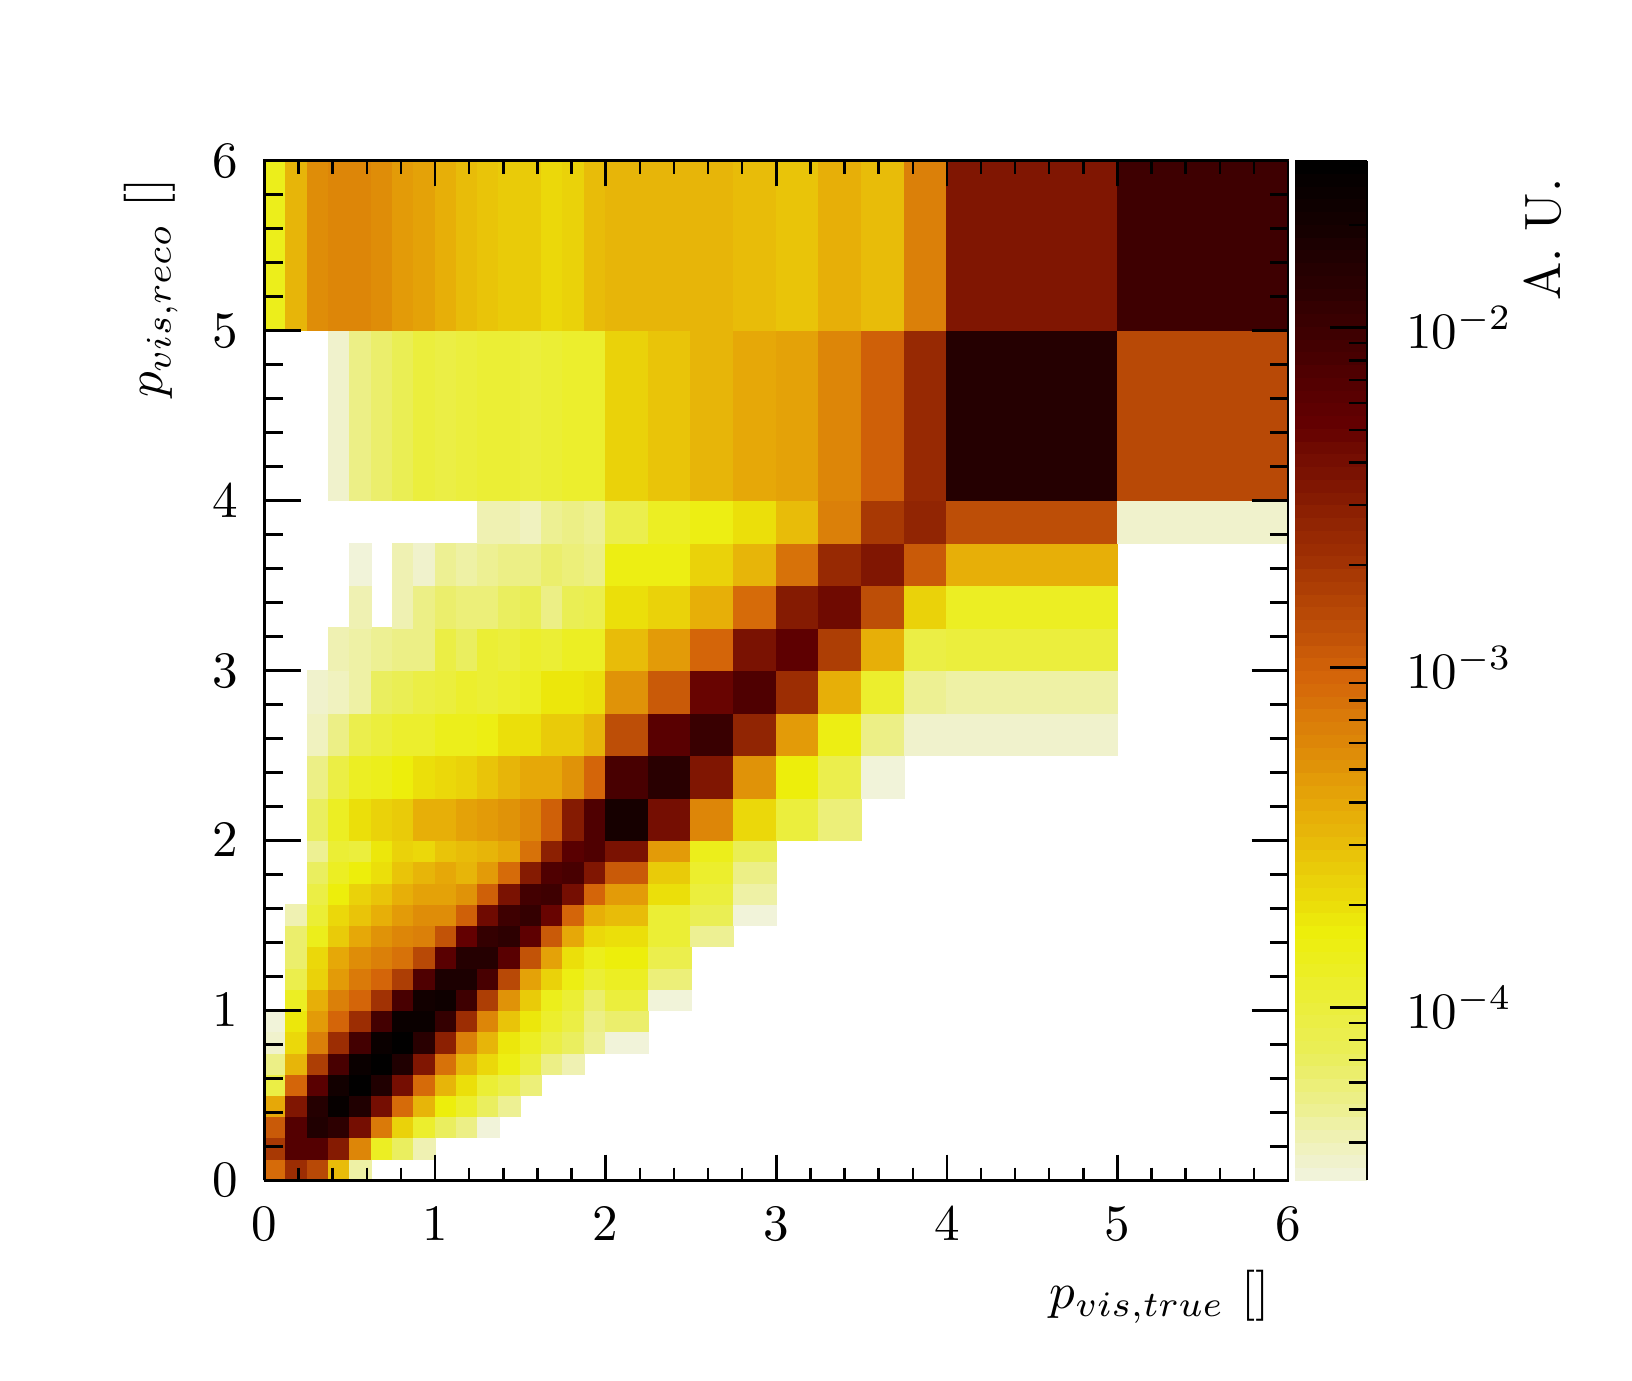
\begin{tikzpicture}
\pgfdeclareplotmark{cross} {
\pgfpathmoveto{\pgfpoint{-0.3\pgfplotmarksize}{\pgfplotmarksize}}
\pgfpathlineto{\pgfpoint{+0.3\pgfplotmarksize}{\pgfplotmarksize}}
\pgfpathlineto{\pgfpoint{+0.3\pgfplotmarksize}{0.3\pgfplotmarksize}}
\pgfpathlineto{\pgfpoint{+1\pgfplotmarksize}{0.3\pgfplotmarksize}}
\pgfpathlineto{\pgfpoint{+1\pgfplotmarksize}{-0.3\pgfplotmarksize}}
\pgfpathlineto{\pgfpoint{+0.3\pgfplotmarksize}{-0.3\pgfplotmarksize}}
\pgfpathlineto{\pgfpoint{+0.3\pgfplotmarksize}{-1.\pgfplotmarksize}}
\pgfpathlineto{\pgfpoint{-0.3\pgfplotmarksize}{-1.\pgfplotmarksize}}
\pgfpathlineto{\pgfpoint{-0.3\pgfplotmarksize}{-0.3\pgfplotmarksize}}
\pgfpathlineto{\pgfpoint{-1.\pgfplotmarksize}{-0.3\pgfplotmarksize}}
\pgfpathlineto{\pgfpoint{-1.\pgfplotmarksize}{0.3\pgfplotmarksize}}
\pgfpathlineto{\pgfpoint{-0.3\pgfplotmarksize}{0.3\pgfplotmarksize}}
\pgfpathclose
\pgfusepathqstroke
}
\pgfdeclareplotmark{cross*} {
\pgfpathmoveto{\pgfpoint{-0.3\pgfplotmarksize}{\pgfplotmarksize}}
\pgfpathlineto{\pgfpoint{+0.3\pgfplotmarksize}{\pgfplotmarksize}}
\pgfpathlineto{\pgfpoint{+0.3\pgfplotmarksize}{0.3\pgfplotmarksize}}
\pgfpathlineto{\pgfpoint{+1\pgfplotmarksize}{0.3\pgfplotmarksize}}
\pgfpathlineto{\pgfpoint{+1\pgfplotmarksize}{-0.3\pgfplotmarksize}}
\pgfpathlineto{\pgfpoint{+0.3\pgfplotmarksize}{-0.3\pgfplotmarksize}}
\pgfpathlineto{\pgfpoint{+0.3\pgfplotmarksize}{-1.\pgfplotmarksize}}
\pgfpathlineto{\pgfpoint{-0.3\pgfplotmarksize}{-1.\pgfplotmarksize}}
\pgfpathlineto{\pgfpoint{-0.3\pgfplotmarksize}{-0.3\pgfplotmarksize}}
\pgfpathlineto{\pgfpoint{-1.\pgfplotmarksize}{-0.3\pgfplotmarksize}}
\pgfpathlineto{\pgfpoint{-1.\pgfplotmarksize}{0.3\pgfplotmarksize}}
\pgfpathlineto{\pgfpoint{-0.3\pgfplotmarksize}{0.3\pgfplotmarksize}}
\pgfpathclose
\pgfusepathqfillstroke
}
\pgfdeclareplotmark{newstar} {
\pgfpathmoveto{\pgfqpoint{0pt}{\pgfplotmarksize}}
\pgfpathlineto{\pgfqpointpolar{44}{0.5\pgfplotmarksize}}
\pgfpathlineto{\pgfqpointpolar{18}{\pgfplotmarksize}}
\pgfpathlineto{\pgfqpointpolar{-20}{0.5\pgfplotmarksize}}
\pgfpathlineto{\pgfqpointpolar{-54}{\pgfplotmarksize}}
\pgfpathlineto{\pgfqpointpolar{-90}{0.5\pgfplotmarksize}}
\pgfpathlineto{\pgfqpointpolar{234}{\pgfplotmarksize}}
\pgfpathlineto{\pgfqpointpolar{198}{0.5\pgfplotmarksize}}
\pgfpathlineto{\pgfqpointpolar{162}{\pgfplotmarksize}}
\pgfpathlineto{\pgfqpointpolar{134}{0.5\pgfplotmarksize}}
\pgfpathclose
\pgfusepathqstroke
}
\pgfdeclareplotmark{newstar*} {
\pgfpathmoveto{\pgfqpoint{0pt}{\pgfplotmarksize}}
\pgfpathlineto{\pgfqpointpolar{44}{0.5\pgfplotmarksize}}
\pgfpathlineto{\pgfqpointpolar{18}{\pgfplotmarksize}}
\pgfpathlineto{\pgfqpointpolar{-20}{0.5\pgfplotmarksize}}
\pgfpathlineto{\pgfqpointpolar{-54}{\pgfplotmarksize}}
\pgfpathlineto{\pgfqpointpolar{-90}{0.5\pgfplotmarksize}}
\pgfpathlineto{\pgfqpointpolar{234}{\pgfplotmarksize}}
\pgfpathlineto{\pgfqpointpolar{198}{0.5\pgfplotmarksize}}
\pgfpathlineto{\pgfqpointpolar{162}{\pgfplotmarksize}}
\pgfpathlineto{\pgfqpointpolar{134}{0.5\pgfplotmarksize}}
\pgfpathclose
\pgfusepathqfillstroke
}
\definecolor{c}{rgb}{1,1,1};
\draw [color=c, fill=c] (0,0) rectangle (20,16.8195);
\draw [color=c, fill=c] (3,2.18653) rectangle (16,15.1375);
\definecolor{c}{rgb}{0,0,0};
\draw [c,line width=0.9] (3,2.18653) -- (3,15.1375) -- (16,15.1375) -- (16,2.18653) -- (3,2.18653);
\definecolor{c}{rgb}{1,1,1};
\draw [color=c, fill=c] (3,2.18653) rectangle (16,15.1375);
\definecolor{c}{rgb}{0,0,0};
\draw [c,line width=0.9] (3,2.18653) -- (3,15.1375) -- (16,15.1375) -- (16,2.18653) -- (3,2.18653);
\definecolor{c}{rgb}{0.83799,0.420711,0.0349265};
\draw [color=c, fill=c] (3,2.18653) rectangle (3.27083,2.45635);
\definecolor{c}{rgb}{0.611765,0.176471,0.0117647};
\draw [color=c, fill=c] (3.27083,2.18653) rectangle (3.54167,2.45635);
\definecolor{c}{rgb}{0.721569,0.286275,0.0235294};
\draw [color=c, fill=c] (3.54167,2.18653) rectangle (3.8125,2.45635);
\definecolor{c}{rgb}{0.909681,0.736029,0.0346814};
\draw [color=c, fill=c] (3.8125,2.18653) rectangle (4.08333,2.45635);
\definecolor{c}{rgb}{0.933839,0.943453,0.645794};
\draw [color=c, fill=c] (4.08333,2.18653) rectangle (4.35417,2.45635);
\definecolor{c}{rgb}{0.659804,0.22451,0.0169118};
\draw [color=c, fill=c] (3,2.45635) rectangle (3.27083,2.72616);
\definecolor{c}{rgb}{0.328676,0,0.00392157};
\draw [color=c, fill=c] (3.27083,2.45635) rectangle (3.54167,2.72616);
\draw [color=c, fill=c] (3.54167,2.45635) rectangle (3.8125,2.72616);
\definecolor{c}{rgb}{0.520956,0.104779,0.00857843};
\draw [color=c, fill=c] (3.8125,2.45635) rectangle (4.08333,2.72616);
\definecolor{c}{rgb}{0.866667,0.527451,0.0333333};
\draw [color=c, fill=c] (4.08333,2.45635) rectangle (4.35417,2.72616);
\definecolor{c}{rgb}{0.926103,0.933333,0.135784};
\draw [color=c, fill=c] (4.35417,2.45635) rectangle (4.625,2.72616);
\definecolor{c}{rgb}{0.917647,0.933333,0.372549};
\draw [color=c, fill=c] (4.625,2.45635) rectangle (4.89583,2.72616);
\definecolor{c}{rgb}{0.936875,0.945351,0.697027};
\draw [color=c, fill=c] (4.89583,2.45635) rectangle (5.16667,2.72616);
\definecolor{c}{rgb}{0.790196,0.354902,0.0308824};
\draw [color=c, fill=c] (3,2.72616) rectangle (3.27083,2.99597);
\definecolor{c}{rgb}{0.328676,0,0.00392157};
\draw [color=c, fill=c] (3.27083,2.72616) rectangle (3.54167,2.99597);
\definecolor{c}{rgb}{0.126838,0,0.00281863};
\draw [color=c, fill=c] (3.54167,2.72616) rectangle (3.8125,2.99597);
\definecolor{c}{rgb}{0.176471,0,0.00392157};
\draw [color=c, fill=c] (3.8125,2.72616) rectangle (4.08333,2.99597);
\definecolor{c}{rgb}{0.458088,0.0551471,0.00637255};
\draw [color=c, fill=c] (4.08333,2.72616) rectangle (4.35417,2.99597);
\definecolor{c}{rgb}{0.853431,0.478186,0.0340686};
\draw [color=c, fill=c] (4.35417,2.72616) rectangle (4.625,2.99597);
\definecolor{c}{rgb}{0.91826,0.821814,0.0383578};
\draw [color=c, fill=c] (4.625,2.72616) rectangle (4.89583,2.99597);
\definecolor{c}{rgb}{0.924632,0.933333,0.176961};
\draw [color=c, fill=c] (4.89583,2.72616) rectangle (5.16667,2.99597);
\definecolor{c}{rgb}{0.917647,0.933333,0.372549};
\draw [color=c, fill=c] (5.16667,2.72616) rectangle (5.4375,2.99597);
\definecolor{c}{rgb}{0.926755,0.939026,0.526249};
\draw [color=c, fill=c] (5.4375,2.72616) rectangle (5.70833,2.99597);
\definecolor{c}{rgb}{0.945984,0.951044,0.850727};
\draw [color=c, fill=c] (5.70833,2.72616) rectangle (5.97917,2.99597);
\definecolor{c}{rgb}{0.901961,0.658824,0.0313726};
\draw [color=c, fill=c] (3,2.99597) rectangle (3.27083,3.26578);
\definecolor{c}{rgb}{0.5,0.0882353,0.00784314};
\draw [color=c, fill=c] (3.27083,2.99597) rectangle (3.54167,3.26578);
\definecolor{c}{rgb}{0.143382,0,0.00318627};
\draw [color=c, fill=c] (3.54167,2.99597) rectangle (3.8125,3.26578);
\definecolor{c}{rgb}{0.0220588,0,0.000490196};
\draw [color=c, fill=c] (3.8125,2.99597) rectangle (4.08333,3.26578);
\definecolor{c}{rgb}{0.126838,0,0.00281863};
\draw [color=c, fill=c] (4.08333,2.99597) rectangle (4.35417,3.26578);
\definecolor{c}{rgb}{0.458088,0.0551471,0.00637255};
\draw [color=c, fill=c] (4.35417,2.99597) rectangle (4.625,3.26578);
\definecolor{c}{rgb}{0.83799,0.420711,0.0349265};
\draw [color=c, fill=c] (4.625,2.99597) rectangle (4.89583,3.26578);
\definecolor{c}{rgb}{0.907108,0.710294,0.0335784};
\draw [color=c, fill=c] (4.89583,2.99597) rectangle (5.16667,3.26578);
\definecolor{c}{rgb}{0.929412,0.933333,0.0431373};
\draw [color=c, fill=c] (5.16667,2.99597) rectangle (5.4375,3.26578);
\definecolor{c}{rgb}{0.924632,0.933333,0.176961};
\draw [color=c, fill=c] (5.4375,2.99597) rectangle (5.70833,3.26578);
\definecolor{c}{rgb}{0.917647,0.933333,0.372549};
\draw [color=c, fill=c] (5.70833,2.99597) rectangle (5.97917,3.26578);
\definecolor{c}{rgb}{0.929791,0.940923,0.577483};
\draw [color=c, fill=c] (5.97917,2.99597) rectangle (6.25,3.26578);
\definecolor{c}{rgb}{0.921324,0.933333,0.269608};
\draw [color=c, fill=c] (3,3.26578) rectangle (3.27083,3.5356);
\definecolor{c}{rgb}{0.831373,0.396078,0.0352941};
\draw [color=c, fill=c] (3.27083,3.26578) rectangle (3.54167,3.5356);
\definecolor{c}{rgb}{0.348529,0,0.00392157};
\draw [color=c, fill=c] (3.54167,3.26578) rectangle (3.8125,3.5356);
\definecolor{c}{rgb}{0.0716912,0,0.00159314};
\draw [color=c, fill=c] (3.8125,3.26578) rectangle (4.08333,3.5356);
\definecolor{c}{rgb}{0.00551471,0,0.000122549};
\draw [color=c, fill=c] (4.08333,3.26578) rectangle (4.35417,3.5356);
\definecolor{c}{rgb}{0.126838,0,0.00281863};
\draw [color=c, fill=c] (4.35417,3.26578) rectangle (4.625,3.5356);
\definecolor{c}{rgb}{0.458088,0.0551471,0.00637255};
\draw [color=c, fill=c] (4.625,3.26578) rectangle (4.89583,3.5356);
\definecolor{c}{rgb}{0.83799,0.420711,0.0349265};
\draw [color=c, fill=c] (4.89583,3.26578) rectangle (5.16667,3.5356);
\definecolor{c}{rgb}{0.907108,0.710294,0.0335784};
\draw [color=c, fill=c] (5.16667,3.26578) rectangle (5.4375,3.5356);
\definecolor{c}{rgb}{0.923407,0.873284,0.0405637};
\draw [color=c, fill=c] (5.4375,3.26578) rectangle (5.70833,3.5356);
\definecolor{c}{rgb}{0.923529,0.933333,0.207843};
\draw [color=c, fill=c] (5.70833,3.26578) rectangle (5.97917,3.5356);
\definecolor{c}{rgb}{0.920221,0.933333,0.30049};
\draw [color=c, fill=c] (5.97917,3.26578) rectangle (6.25,3.5356);
\definecolor{c}{rgb}{0.923719,0.937128,0.475016};
\draw [color=c, fill=c] (6.25,3.26578) rectangle (6.52083,3.5356);
\definecolor{c}{rgb}{0.926755,0.939026,0.526249};
\draw [color=c, fill=c] (3,3.5356) rectangle (3.27083,3.80541);
\definecolor{c}{rgb}{0.907108,0.710294,0.0335784};
\draw [color=c, fill=c] (3.27083,3.5356) rectangle (3.54167,3.80541);
\definecolor{c}{rgb}{0.680392,0.245098,0.0191176};
\draw [color=c, fill=c] (3.54167,3.5356) rectangle (3.8125,3.80541);
\definecolor{c}{rgb}{0.282353,0,0.00392157};
\draw [color=c, fill=c] (3.8125,3.5356) rectangle (4.08333,3.80541);
\definecolor{c}{rgb}{0.0386029,0,0.000857843};
\draw [color=c, fill=c] (4.08333,3.5356) rectangle (4.35417,3.80541);
\definecolor{c}{rgb}{0.00551471,0,0.000122549};
\draw [color=c, fill=c] (4.35417,3.5356) rectangle (4.625,3.80541);
\definecolor{c}{rgb}{0.126838,0,0.00281863};
\draw [color=c, fill=c] (4.625,3.5356) rectangle (4.89583,3.80541);
\definecolor{c}{rgb}{0.5,0.0882353,0.00784314};
\draw [color=c, fill=c] (4.89583,3.5356) rectangle (5.16667,3.80541);
\definecolor{c}{rgb}{0.844608,0.445343,0.0345588};
\draw [color=c, fill=c] (5.16667,3.5356) rectangle (5.4375,3.80541);
\definecolor{c}{rgb}{0.907108,0.710294,0.0335784};
\draw [color=c, fill=c] (5.4375,3.5356) rectangle (5.70833,3.80541);
\definecolor{c}{rgb}{0.920833,0.847549,0.0394608};
\draw [color=c, fill=c] (5.70833,3.5356) rectangle (5.97917,3.80541);
\definecolor{c}{rgb}{0.928309,0.933333,0.0740196};
\draw [color=c, fill=c] (5.97917,3.5356) rectangle (6.25,3.80541);
\definecolor{c}{rgb}{0.922426,0.933333,0.238725};
\draw [color=c, fill=c] (6.25,3.5356) rectangle (6.52083,3.80541);
\definecolor{c}{rgb}{0.926755,0.939026,0.526249};
\draw [color=c, fill=c] (6.52083,3.5356) rectangle (6.79167,3.80541);
\definecolor{c}{rgb}{0.936875,0.945351,0.697027};
\draw [color=c, fill=c] (6.79167,3.5356) rectangle (7.0625,3.80541);
\definecolor{c}{rgb}{0.942948,0.949146,0.799494};
\draw [color=c, fill=c] (3,3.80541) rectangle (3.27083,4.07522);
\definecolor{c}{rgb}{0.920833,0.847549,0.0394608};
\draw [color=c, fill=c] (3.27083,3.80541) rectangle (3.54167,4.07522);
\definecolor{c}{rgb}{0.860049,0.502819,0.033701};
\draw [color=c, fill=c] (3.54167,3.80541) rectangle (3.8125,4.07522);
\definecolor{c}{rgb}{0.611765,0.176471,0.0117647};
\draw [color=c, fill=c] (3.8125,3.80541) rectangle (4.08333,4.07522);
\definecolor{c}{rgb}{0.2625,0,0.00392157};
\draw [color=c, fill=c] (4.08333,3.80541) rectangle (4.35417,4.07522);
\definecolor{c}{rgb}{0.0386029,0,0.000857843};
\draw [color=c, fill=c] (4.35417,3.80541) rectangle (4.625,4.07522);
\definecolor{c}{rgb}{0.00551471,0,0.000122549};
\draw [color=c, fill=c] (4.625,3.80541) rectangle (4.89583,4.07522);
\definecolor{c}{rgb}{0.159926,0,0.00355392};
\draw [color=c, fill=c] (4.89583,3.80541) rectangle (5.16667,4.07522);
\definecolor{c}{rgb}{0.548897,0.126838,0.00955882};
\draw [color=c, fill=c] (5.16667,3.80541) rectangle (5.4375,4.07522);
\definecolor{c}{rgb}{0.860049,0.502819,0.033701};
\draw [color=c, fill=c] (5.4375,3.80541) rectangle (5.70833,4.07522);
\definecolor{c}{rgb}{0.907108,0.710294,0.0335784};
\draw [color=c, fill=c] (5.70833,3.80541) rectangle (5.97917,4.07522);
\definecolor{c}{rgb}{0.926838,0.907598,0.0420343};
\draw [color=c, fill=c] (5.97917,3.80541) rectangle (6.25,4.07522);
\definecolor{c}{rgb}{0.926103,0.933333,0.135784};
\draw [color=c, fill=c] (6.25,3.80541) rectangle (6.52083,4.07522);
\definecolor{c}{rgb}{0.921324,0.933333,0.269608};
\draw [color=c, fill=c] (6.52083,3.80541) rectangle (6.79167,4.07522);
\definecolor{c}{rgb}{0.917647,0.933333,0.372549};
\draw [color=c, fill=c] (6.79167,3.80541) rectangle (7.0625,4.07522);
\definecolor{c}{rgb}{0.929791,0.940923,0.577483};
\draw [color=c, fill=c] (7.0625,3.80541) rectangle (7.33333,4.07522);
\definecolor{c}{rgb}{0.945984,0.951044,0.850727};
\draw [color=c, fill=c] (7.33333,3.80541) rectangle (7.875,4.07522);
\draw [color=c, fill=c] (3,4.07522) rectangle (3.27083,4.34503);
\definecolor{c}{rgb}{0.926838,0.907598,0.0420343};
\draw [color=c, fill=c] (3.27083,4.07522) rectangle (3.54167,4.34503);
\definecolor{c}{rgb}{0.888726,0.609559,0.0321078};
\draw [color=c, fill=c] (3.54167,4.07522) rectangle (3.8125,4.34503);
\definecolor{c}{rgb}{0.831373,0.396078,0.0352941};
\draw [color=c, fill=c] (3.8125,4.07522) rectangle (4.08333,4.34503);
\definecolor{c}{rgb}{0.611765,0.176471,0.0117647};
\draw [color=c, fill=c] (4.08333,4.07522) rectangle (4.35417,4.34503);
\definecolor{c}{rgb}{0.2625,0,0.00392157};
\draw [color=c, fill=c] (4.35417,4.07522) rectangle (4.625,4.34503);
\definecolor{c}{rgb}{0.0386029,0,0.000857843};
\draw [color=c, fill=c] (4.625,4.07522) rectangle (4.89583,4.34503);
\draw [color=c, fill=c] (4.89583,4.07522) rectangle (5.16667,4.34503);
\definecolor{c}{rgb}{0.202941,0,0.00392157};
\draw [color=c, fill=c] (5.16667,4.07522) rectangle (5.4375,4.34503);
\definecolor{c}{rgb}{0.611765,0.176471,0.0117647};
\draw [color=c, fill=c] (5.4375,4.07522) rectangle (5.70833,4.34503);
\definecolor{c}{rgb}{0.866667,0.527451,0.0333333};
\draw [color=c, fill=c] (5.70833,4.07522) rectangle (5.97917,4.34503);
\definecolor{c}{rgb}{0.913113,0.770343,0.036152};
\draw [color=c, fill=c] (5.97917,4.07522) rectangle (6.25,4.34503);
\definecolor{c}{rgb}{0.926838,0.907598,0.0420343};
\draw [color=c, fill=c] (6.25,4.07522) rectangle (6.52083,4.34503);
\definecolor{c}{rgb}{0.924632,0.933333,0.176961};
\draw [color=c, fill=c] (6.52083,4.07522) rectangle (6.79167,4.34503);
\definecolor{c}{rgb}{0.921324,0.933333,0.269608};
\draw [color=c, fill=c] (6.79167,4.07522) rectangle (7.0625,4.34503);
\definecolor{c}{rgb}{0.926755,0.939026,0.526249};
\draw [color=c, fill=c] (7.0625,4.07522) rectangle (7.33333,4.34503);
\definecolor{c}{rgb}{0.920683,0.935231,0.423782};
\draw [color=c, fill=c] (7.33333,4.07522) rectangle (7.875,4.34503);
\definecolor{c}{rgb}{0.926103,0.933333,0.135784};
\draw [color=c, fill=c] (3.27083,4.34503) rectangle (3.54167,4.61485);
\definecolor{c}{rgb}{0.904534,0.684559,0.0324755};
\draw [color=c, fill=c] (3.54167,4.34503) rectangle (3.8125,4.61485);
\definecolor{c}{rgb}{0.860049,0.502819,0.033701};
\draw [color=c, fill=c] (3.8125,4.34503) rectangle (4.08333,4.61485);
\definecolor{c}{rgb}{0.831373,0.396078,0.0352941};
\draw [color=c, fill=c] (4.08333,4.34503) rectangle (4.35417,4.61485);
\definecolor{c}{rgb}{0.632353,0.197059,0.0139706};
\draw [color=c, fill=c] (4.35417,4.34503) rectangle (4.625,4.61485);
\definecolor{c}{rgb}{0.282353,0,0.00392157};
\draw [color=c, fill=c] (4.625,4.34503) rectangle (4.89583,4.61485);
\definecolor{c}{rgb}{0.0716912,0,0.00159314};
\draw [color=c, fill=c] (4.89583,4.34503) rectangle (5.16667,4.61485);
\definecolor{c}{rgb}{0.0551471,0,0.00122549};
\draw [color=c, fill=c] (5.16667,4.34503) rectangle (5.4375,4.61485);
\definecolor{c}{rgb}{0.242647,0,0.00392157};
\draw [color=c, fill=c] (5.4375,4.34503) rectangle (5.70833,4.61485);
\definecolor{c}{rgb}{0.680392,0.245098,0.0191176};
\draw [color=c, fill=c] (5.70833,4.34503) rectangle (5.97917,4.61485);
\definecolor{c}{rgb}{0.879902,0.576716,0.032598};
\draw [color=c, fill=c] (5.97917,4.34503) rectangle (6.25,4.61485);
\definecolor{c}{rgb}{0.915686,0.796078,0.0372549};
\draw [color=c, fill=c] (6.25,4.34503) rectangle (6.52083,4.61485);
\definecolor{c}{rgb}{0.927206,0.933333,0.104902};
\draw [color=c, fill=c] (6.52083,4.34503) rectangle (6.79167,4.61485);
\definecolor{c}{rgb}{0.923529,0.933333,0.207843};
\draw [color=c, fill=c] (6.79167,4.34503) rectangle (7.0625,4.61485);
\definecolor{c}{rgb}{0.920683,0.935231,0.423782};
\draw [color=c, fill=c] (7.0625,4.34503) rectangle (7.33333,4.61485);
\definecolor{c}{rgb}{0.922426,0.933333,0.238725};
\draw [color=c, fill=c] (7.33333,4.34503) rectangle (7.875,4.61485);
\definecolor{c}{rgb}{0.945984,0.951044,0.850727};
\draw [color=c, fill=c] (7.875,4.34503) rectangle (8.41667,4.61485);
\definecolor{c}{rgb}{0.920221,0.933333,0.30049};
\draw [color=c, fill=c] (3.27083,4.61485) rectangle (3.54167,4.88466);
\definecolor{c}{rgb}{0.91826,0.821814,0.0383578};
\draw [color=c, fill=c] (3.54167,4.61485) rectangle (3.8125,4.88466);
\definecolor{c}{rgb}{0.888726,0.609559,0.0321078};
\draw [color=c, fill=c] (3.8125,4.61485) rectangle (4.08333,4.88466);
\definecolor{c}{rgb}{0.853431,0.478186,0.0340686};
\draw [color=c, fill=c] (4.08333,4.61485) rectangle (4.35417,4.88466);
\definecolor{c}{rgb}{0.831373,0.396078,0.0352941};
\draw [color=c, fill=c] (4.35417,4.61485) rectangle (4.625,4.88466);
\definecolor{c}{rgb}{0.680392,0.245098,0.0191176};
\draw [color=c, fill=c] (4.625,4.61485) rectangle (4.89583,4.88466);
\definecolor{c}{rgb}{0.308824,0,0.00392157};
\draw [color=c, fill=c] (4.89583,4.61485) rectangle (5.16667,4.88466);
\definecolor{c}{rgb}{0.110294,0,0.00245098};
\draw [color=c, fill=c] (5.16667,4.61485) rectangle (5.4375,4.88466);
\draw [color=c, fill=c] (5.4375,4.61485) rectangle (5.70833,4.88466);
\definecolor{c}{rgb}{0.282353,0,0.00392157};
\draw [color=c, fill=c] (5.70833,4.61485) rectangle (5.97917,4.88466);
\definecolor{c}{rgb}{0.721569,0.286275,0.0235294};
\draw [color=c, fill=c] (5.97917,4.61485) rectangle (6.25,4.88466);
\definecolor{c}{rgb}{0.895343,0.634191,0.0317402};
\draw [color=c, fill=c] (6.25,4.61485) rectangle (6.52083,4.88466);
\definecolor{c}{rgb}{0.91826,0.821814,0.0383578};
\draw [color=c, fill=c] (6.52083,4.61485) rectangle (6.79167,4.88466);
\definecolor{c}{rgb}{0.928309,0.933333,0.0740196};
\draw [color=c, fill=c] (6.79167,4.61485) rectangle (7.0625,4.88466);
\definecolor{c}{rgb}{0.923529,0.933333,0.207843};
\draw [color=c, fill=c] (7.0625,4.61485) rectangle (7.33333,4.88466);
\definecolor{c}{rgb}{0.926103,0.933333,0.135784};
\draw [color=c, fill=c] (7.33333,4.61485) rectangle (7.875,4.88466);
\definecolor{c}{rgb}{0.923719,0.937128,0.475016};
\draw [color=c, fill=c] (7.875,4.61485) rectangle (8.41667,4.88466);
\definecolor{c}{rgb}{0.920683,0.935231,0.423782};
\draw [color=c, fill=c] (3.27083,4.88466) rectangle (3.54167,5.15447);
\definecolor{c}{rgb}{0.920833,0.847549,0.0394608};
\draw [color=c, fill=c] (3.54167,4.88466) rectangle (3.8125,5.15447);
\definecolor{c}{rgb}{0.901961,0.658824,0.0313726};
\draw [color=c, fill=c] (3.8125,4.88466) rectangle (4.08333,5.15447);
\definecolor{c}{rgb}{0.873284,0.552083,0.0329657};
\draw [color=c, fill=c] (4.08333,4.88466) rectangle (4.35417,5.15447);
\definecolor{c}{rgb}{0.860049,0.502819,0.033701};
\draw [color=c, fill=c] (4.35417,4.88466) rectangle (4.625,5.15447);
\definecolor{c}{rgb}{0.844608,0.445343,0.0345588};
\draw [color=c, fill=c] (4.625,4.88466) rectangle (4.89583,5.15447);
\definecolor{c}{rgb}{0.721569,0.286275,0.0235294};
\draw [color=c, fill=c] (4.89583,4.88466) rectangle (5.16667,5.15447);
\definecolor{c}{rgb}{0.348529,0,0.00392157};
\draw [color=c, fill=c] (5.16667,4.88466) rectangle (5.4375,5.15447);
\definecolor{c}{rgb}{0.143382,0,0.00318627};
\draw [color=c, fill=c] (5.4375,4.88466) rectangle (5.70833,5.15447);
\draw [color=c, fill=c] (5.70833,4.88466) rectangle (5.97917,5.15447);
\definecolor{c}{rgb}{0.348529,0,0.00392157};
\draw [color=c, fill=c] (5.97917,4.88466) rectangle (6.25,5.15447);
\definecolor{c}{rgb}{0.762745,0.327451,0.0279412};
\draw [color=c, fill=c] (6.25,4.88466) rectangle (6.52083,5.15447);
\definecolor{c}{rgb}{0.895343,0.634191,0.0317402};
\draw [color=c, fill=c] (6.52083,4.88466) rectangle (6.79167,5.15447);
\definecolor{c}{rgb}{0.923407,0.873284,0.0405637};
\draw [color=c, fill=c] (6.79167,4.88466) rectangle (7.0625,5.15447);
\definecolor{c}{rgb}{0.927206,0.933333,0.104902};
\draw [color=c, fill=c] (7.0625,4.88466) rectangle (7.33333,5.15447);
\definecolor{c}{rgb}{0.929412,0.933333,0.0431373};
\draw [color=c, fill=c] (7.33333,4.88466) rectangle (7.875,5.15447);
\definecolor{c}{rgb}{0.920221,0.933333,0.30049};
\draw [color=c, fill=c] (7.875,4.88466) rectangle (8.41667,5.15447);
\definecolor{c}{rgb}{0.920683,0.935231,0.423782};
\draw [color=c, fill=c] (3.27083,5.15447) rectangle (3.54167,5.42428);
\definecolor{c}{rgb}{0.927206,0.933333,0.104902};
\draw [color=c, fill=c] (3.54167,5.15447) rectangle (3.8125,5.42428);
\definecolor{c}{rgb}{0.915686,0.796078,0.0372549};
\draw [color=c, fill=c] (3.8125,5.15447) rectangle (4.08333,5.42428);
\definecolor{c}{rgb}{0.901961,0.658824,0.0313726};
\draw [color=c, fill=c] (4.08333,5.15447) rectangle (4.35417,5.42428);
\definecolor{c}{rgb}{0.879902,0.576716,0.032598};
\draw [color=c, fill=c] (4.35417,5.15447) rectangle (4.625,5.42428);
\definecolor{c}{rgb}{0.866667,0.527451,0.0333333};
\draw [color=c, fill=c] (4.625,5.15447) rectangle (4.89583,5.42428);
\definecolor{c}{rgb}{0.860049,0.502819,0.033701};
\draw [color=c, fill=c] (4.89583,5.15447) rectangle (5.16667,5.42428);
\definecolor{c}{rgb}{0.762745,0.327451,0.0279412};
\draw [color=c, fill=c] (5.16667,5.15447) rectangle (5.4375,5.42428);
\definecolor{c}{rgb}{0.388235,0,0.00392157};
\draw [color=c, fill=c] (5.4375,5.15447) rectangle (5.70833,5.42428);
\definecolor{c}{rgb}{0.202941,0,0.00392157};
\draw [color=c, fill=c] (5.70833,5.15447) rectangle (5.97917,5.42428);
\definecolor{c}{rgb}{0.176471,0,0.00392157};
\draw [color=c, fill=c] (5.97917,5.15447) rectangle (6.25,5.42428);
\definecolor{c}{rgb}{0.368382,0,0.00392157};
\draw [color=c, fill=c] (6.25,5.15447) rectangle (6.52083,5.42428);
\definecolor{c}{rgb}{0.790196,0.354902,0.0308824};
\draw [color=c, fill=c] (6.52083,5.15447) rectangle (6.79167,5.42428);
\definecolor{c}{rgb}{0.901961,0.658824,0.0313726};
\draw [color=c, fill=c] (6.79167,5.15447) rectangle (7.0625,5.42428);
\definecolor{c}{rgb}{0.920833,0.847549,0.0394608};
\draw [color=c, fill=c] (7.0625,5.15447) rectangle (7.33333,5.42428);
\definecolor{c}{rgb}{0.923407,0.873284,0.0405637};
\draw [color=c, fill=c] (7.33333,5.15447) rectangle (7.875,5.42428);
\definecolor{c}{rgb}{0.923529,0.933333,0.207843};
\draw [color=c, fill=c] (7.875,5.15447) rectangle (8.41667,5.42428);
\definecolor{c}{rgb}{0.929791,0.940923,0.577483};
\draw [color=c, fill=c] (8.41667,5.15447) rectangle (8.95833,5.42428);
\definecolor{c}{rgb}{0.936875,0.945351,0.697027};
\draw [color=c, fill=c] (3.27083,5.42428) rectangle (3.54167,5.6941);
\definecolor{c}{rgb}{0.923529,0.933333,0.207843};
\draw [color=c, fill=c] (3.54167,5.42428) rectangle (3.8125,5.6941);
\definecolor{c}{rgb}{0.920833,0.847549,0.0394608};
\draw [color=c, fill=c] (3.8125,5.42428) rectangle (4.08333,5.6941);
\definecolor{c}{rgb}{0.913113,0.770343,0.036152};
\draw [color=c, fill=c] (4.08333,5.42428) rectangle (4.35417,5.6941);
\definecolor{c}{rgb}{0.904534,0.684559,0.0324755};
\draw [color=c, fill=c] (4.35417,5.42428) rectangle (4.625,5.6941);
\definecolor{c}{rgb}{0.888726,0.609559,0.0321078};
\draw [color=c, fill=c] (4.625,5.42428) rectangle (4.89583,5.6941);
\definecolor{c}{rgb}{0.873284,0.552083,0.0329657};
\draw [color=c, fill=c] (4.89583,5.42428) rectangle (5.16667,5.6941);
\draw [color=c, fill=c] (5.16667,5.42428) rectangle (5.4375,5.6941);
\definecolor{c}{rgb}{0.810784,0.37549,0.0330882};
\draw [color=c, fill=c] (5.4375,5.42428) rectangle (5.70833,5.6941);
\definecolor{c}{rgb}{0.437132,0.0386029,0.00563726};
\draw [color=c, fill=c] (5.70833,5.42428) rectangle (5.97917,5.6941);
\definecolor{c}{rgb}{0.242647,0,0.00392157};
\draw [color=c, fill=c] (5.97917,5.42428) rectangle (6.25,5.6941);
\definecolor{c}{rgb}{0.202941,0,0.00392157};
\draw [color=c, fill=c] (6.25,5.42428) rectangle (6.52083,5.6941);
\definecolor{c}{rgb}{0.409191,0.0165441,0.00465686};
\draw [color=c, fill=c] (6.52083,5.42428) rectangle (6.79167,5.6941);
\definecolor{c}{rgb}{0.831373,0.396078,0.0352941};
\draw [color=c, fill=c] (6.79167,5.42428) rectangle (7.0625,5.6941);
\definecolor{c}{rgb}{0.904534,0.684559,0.0324755};
\draw [color=c, fill=c] (7.0625,5.42428) rectangle (7.33333,5.6941);
\definecolor{c}{rgb}{0.909681,0.736029,0.0346814};
\draw [color=c, fill=c] (7.33333,5.42428) rectangle (7.875,5.6941);
\definecolor{c}{rgb}{0.923529,0.933333,0.207843};
\draw [color=c, fill=c] (7.875,5.42428) rectangle (8.41667,5.6941);
\definecolor{c}{rgb}{0.919118,0.933333,0.331373};
\draw [color=c, fill=c] (8.41667,5.42428) rectangle (8.95833,5.6941);
\definecolor{c}{rgb}{0.945984,0.951044,0.850727};
\draw [color=c, fill=c] (8.95833,5.42428) rectangle (9.5,5.6941);
\definecolor{c}{rgb}{0.921324,0.933333,0.269608};
\draw [color=c, fill=c] (3.54167,5.6941) rectangle (3.8125,5.96391);
\definecolor{c}{rgb}{0.929412,0.933333,0.0431373};
\draw [color=c, fill=c] (3.8125,5.6941) rectangle (4.08333,5.96391);
\definecolor{c}{rgb}{0.91826,0.821814,0.0383578};
\draw [color=c, fill=c] (4.08333,5.6941) rectangle (4.35417,5.96391);
\definecolor{c}{rgb}{0.913113,0.770343,0.036152};
\draw [color=c, fill=c] (4.35417,5.6941) rectangle (4.625,5.96391);
\definecolor{c}{rgb}{0.904534,0.684559,0.0324755};
\draw [color=c, fill=c] (4.625,5.6941) rectangle (4.89583,5.96391);
\definecolor{c}{rgb}{0.895343,0.634191,0.0317402};
\draw [color=c, fill=c] (4.89583,5.6941) rectangle (5.16667,5.96391);
\draw [color=c, fill=c] (5.16667,5.6941) rectangle (5.4375,5.96391);
\definecolor{c}{rgb}{0.879902,0.576716,0.032598};
\draw [color=c, fill=c] (5.4375,5.6941) rectangle (5.70833,5.96391);
\definecolor{c}{rgb}{0.810784,0.37549,0.0330882};
\draw [color=c, fill=c] (5.70833,5.6941) rectangle (5.97917,5.96391);
\definecolor{c}{rgb}{0.479044,0.0716912,0.00710784};
\draw [color=c, fill=c] (5.97917,5.6941) rectangle (6.25,5.96391);
\definecolor{c}{rgb}{0.2625,0,0.00392157};
\draw [color=c, fill=c] (6.25,5.6941) rectangle (6.52083,5.96391);
\definecolor{c}{rgb}{0.242647,0,0.00392157};
\draw [color=c, fill=c] (6.52083,5.6941) rectangle (6.79167,5.96391);
\definecolor{c}{rgb}{0.458088,0.0551471,0.00637255};
\draw [color=c, fill=c] (6.79167,5.6941) rectangle (7.0625,5.96391);
\definecolor{c}{rgb}{0.831373,0.396078,0.0352941};
\draw [color=c, fill=c] (7.0625,5.6941) rectangle (7.33333,5.96391);
\definecolor{c}{rgb}{0.888726,0.609559,0.0321078};
\draw [color=c, fill=c] (7.33333,5.6941) rectangle (7.875,5.96391);
\definecolor{c}{rgb}{0.923407,0.873284,0.0405637};
\draw [color=c, fill=c] (7.875,5.6941) rectangle (8.41667,5.96391);
\definecolor{c}{rgb}{0.922426,0.933333,0.238725};
\draw [color=c, fill=c] (8.41667,5.6941) rectangle (8.95833,5.96391);
\definecolor{c}{rgb}{0.933839,0.943453,0.645794};
\draw [color=c, fill=c] (8.95833,5.6941) rectangle (9.5,5.96391);
\definecolor{c}{rgb}{0.917647,0.933333,0.372549};
\draw [color=c, fill=c] (3.54167,5.96391) rectangle (3.8125,6.23372);
\definecolor{c}{rgb}{0.926103,0.933333,0.135784};
\draw [color=c, fill=c] (3.8125,5.96391) rectangle (4.08333,6.23372);
\definecolor{c}{rgb}{0.929412,0.933333,0.0431373};
\draw [color=c, fill=c] (4.08333,5.96391) rectangle (4.35417,6.23372);
\definecolor{c}{rgb}{0.923407,0.873284,0.0405637};
\draw [color=c, fill=c] (4.35417,5.96391) rectangle (4.625,6.23372);
\definecolor{c}{rgb}{0.913113,0.770343,0.036152};
\draw [color=c, fill=c] (4.625,5.96391) rectangle (4.89583,6.23372);
\definecolor{c}{rgb}{0.907108,0.710294,0.0335784};
\draw [color=c, fill=c] (4.89583,5.96391) rectangle (5.16667,6.23372);
\definecolor{c}{rgb}{0.901961,0.658824,0.0313726};
\draw [color=c, fill=c] (5.16667,5.96391) rectangle (5.4375,6.23372);
\definecolor{c}{rgb}{0.907108,0.710294,0.0335784};
\draw [color=c, fill=c] (5.4375,5.96391) rectangle (5.70833,6.23372);
\definecolor{c}{rgb}{0.888726,0.609559,0.0321078};
\draw [color=c, fill=c] (5.70833,5.96391) rectangle (5.97917,6.23372);
\definecolor{c}{rgb}{0.83799,0.420711,0.0349265};
\draw [color=c, fill=c] (5.97917,5.96391) rectangle (6.25,6.23372);
\definecolor{c}{rgb}{0.520956,0.104779,0.00857843};
\draw [color=c, fill=c] (6.25,5.96391) rectangle (6.52083,6.23372);
\definecolor{c}{rgb}{0.308824,0,0.00392157};
\draw [color=c, fill=c] (6.52083,5.96391) rectangle (6.79167,6.23372);
\definecolor{c}{rgb}{0.282353,0,0.00392157};
\draw [color=c, fill=c] (6.79167,5.96391) rectangle (7.0625,6.23372);
\definecolor{c}{rgb}{0.5,0.0882353,0.00784314};
\draw [color=c, fill=c] (7.0625,5.96391) rectangle (7.33333,6.23372);
\definecolor{c}{rgb}{0.790196,0.354902,0.0308824};
\draw [color=c, fill=c] (7.33333,5.96391) rectangle (7.875,6.23372);
\definecolor{c}{rgb}{0.915686,0.796078,0.0372549};
\draw [color=c, fill=c] (7.875,5.96391) rectangle (8.41667,6.23372);
\definecolor{c}{rgb}{0.924632,0.933333,0.176961};
\draw [color=c, fill=c] (8.41667,5.96391) rectangle (8.95833,6.23372);
\definecolor{c}{rgb}{0.926755,0.939026,0.526249};
\draw [color=c, fill=c] (8.95833,5.96391) rectangle (9.5,6.23372);
\definecolor{c}{rgb}{0.929791,0.940923,0.577483};
\draw [color=c, fill=c] (3.54167,6.23372) rectangle (3.8125,6.50353);
\definecolor{c}{rgb}{0.923529,0.933333,0.207843};
\draw [color=c, fill=c] (3.8125,6.23372) rectangle (4.08333,6.50353);
\definecolor{c}{rgb}{0.922426,0.933333,0.238725};
\draw [color=c, fill=c] (4.08333,6.23372) rectangle (4.35417,6.50353);
\definecolor{c}{rgb}{0.926838,0.907598,0.0420343};
\draw [color=c, fill=c] (4.35417,6.23372) rectangle (4.625,6.50353);
\definecolor{c}{rgb}{0.91826,0.821814,0.0383578};
\draw [color=c, fill=c] (4.625,6.23372) rectangle (4.89583,6.50353);
\definecolor{c}{rgb}{0.920833,0.847549,0.0394608};
\draw [color=c, fill=c] (4.89583,6.23372) rectangle (5.16667,6.50353);
\definecolor{c}{rgb}{0.913113,0.770343,0.036152};
\draw [color=c, fill=c] (5.16667,6.23372) rectangle (5.4375,6.50353);
\definecolor{c}{rgb}{0.909681,0.736029,0.0346814};
\draw [color=c, fill=c] (5.4375,6.23372) rectangle (5.70833,6.50353);
\definecolor{c}{rgb}{0.907108,0.710294,0.0335784};
\draw [color=c, fill=c] (5.70833,6.23372) rectangle (5.97917,6.50353);
\definecolor{c}{rgb}{0.901961,0.658824,0.0313726};
\draw [color=c, fill=c] (5.97917,6.23372) rectangle (6.25,6.50353);
\definecolor{c}{rgb}{0.844608,0.445343,0.0345588};
\draw [color=c, fill=c] (6.25,6.23372) rectangle (6.52083,6.50353);
\definecolor{c}{rgb}{0.548897,0.126838,0.00955882};
\draw [color=c, fill=c] (6.52083,6.23372) rectangle (6.79167,6.50353);
\definecolor{c}{rgb}{0.348529,0,0.00392157};
\draw [color=c, fill=c] (6.79167,6.23372) rectangle (7.0625,6.50353);
\definecolor{c}{rgb}{0.308824,0,0.00392157};
\draw [color=c, fill=c] (7.0625,6.23372) rectangle (7.33333,6.50353);
\definecolor{c}{rgb}{0.479044,0.0716912,0.00710784};
\draw [color=c, fill=c] (7.33333,6.23372) rectangle (7.875,6.50353);
\definecolor{c}{rgb}{0.888726,0.609559,0.0321078};
\draw [color=c, fill=c] (7.875,6.23372) rectangle (8.41667,6.50353);
\definecolor{c}{rgb}{0.927206,0.933333,0.104902};
\draw [color=c, fill=c] (8.41667,6.23372) rectangle (8.95833,6.50353);
\definecolor{c}{rgb}{0.919118,0.933333,0.331373};
\draw [color=c, fill=c] (8.95833,6.23372) rectangle (9.5,6.50353);
\definecolor{c}{rgb}{0.917647,0.933333,0.372549};
\draw [color=c, fill=c] (3.54167,6.50353) rectangle (3.8125,7.04316);
\definecolor{c}{rgb}{0.926103,0.933333,0.135784};
\draw [color=c, fill=c] (3.8125,6.50353) rectangle (4.08333,7.04316);
\definecolor{c}{rgb}{0.923407,0.873284,0.0405637};
\draw [color=c, fill=c] (4.08333,6.50353) rectangle (4.35417,7.04316);
\definecolor{c}{rgb}{0.91826,0.821814,0.0383578};
\draw [color=c, fill=c] (4.35417,6.50353) rectangle (4.625,7.04316);
\definecolor{c}{rgb}{0.915686,0.796078,0.0372549};
\draw [color=c, fill=c] (4.625,6.50353) rectangle (4.89583,7.04316);
\definecolor{c}{rgb}{0.904534,0.684559,0.0324755};
\draw [color=c, fill=c] (4.89583,6.50353) rectangle (5.16667,7.04316);
\draw [color=c, fill=c] (5.16667,6.50353) rectangle (5.4375,7.04316);
\definecolor{c}{rgb}{0.895343,0.634191,0.0317402};
\draw [color=c, fill=c] (5.4375,6.50353) rectangle (5.70833,7.04316);
\definecolor{c}{rgb}{0.888726,0.609559,0.0321078};
\draw [color=c, fill=c] (5.70833,6.50353) rectangle (5.97917,7.04316);
\definecolor{c}{rgb}{0.879902,0.576716,0.032598};
\draw [color=c, fill=c] (5.97917,6.50353) rectangle (6.25,7.04316);
\definecolor{c}{rgb}{0.866667,0.527451,0.0333333};
\draw [color=c, fill=c] (6.25,6.50353) rectangle (6.52083,7.04316);
\definecolor{c}{rgb}{0.810784,0.37549,0.0330882};
\draw [color=c, fill=c] (6.52083,6.50353) rectangle (6.79167,7.04316);
\definecolor{c}{rgb}{0.520956,0.104779,0.00857843};
\draw [color=c, fill=c] (6.79167,6.50353) rectangle (7.0625,7.04316);
\definecolor{c}{rgb}{0.308824,0,0.00392157};
\draw [color=c, fill=c] (7.0625,6.50353) rectangle (7.33333,7.04316);
\definecolor{c}{rgb}{0.0882353,0,0.00196078};
\draw [color=c, fill=c] (7.33333,6.50353) rectangle (7.875,7.04316);
\definecolor{c}{rgb}{0.458088,0.0551471,0.00637255};
\draw [color=c, fill=c] (7.875,6.50353) rectangle (8.41667,7.04316);
\definecolor{c}{rgb}{0.866667,0.527451,0.0333333};
\draw [color=c, fill=c] (8.41667,6.50353) rectangle (8.95833,7.04316);
\definecolor{c}{rgb}{0.920833,0.847549,0.0394608};
\draw [color=c, fill=c] (8.95833,6.50353) rectangle (9.5,7.04316);
\definecolor{c}{rgb}{0.922426,0.933333,0.238725};
\draw [color=c, fill=c] (9.5,6.50353) rectangle (10.0417,7.04316);
\definecolor{c}{rgb}{0.923719,0.937128,0.475016};
\draw [color=c, fill=c] (10.0417,6.50353) rectangle (10.5833,7.04316);
\definecolor{c}{rgb}{0.926755,0.939026,0.526249};
\draw [color=c, fill=c] (3.54167,7.04316) rectangle (3.8125,7.58278);
\definecolor{c}{rgb}{0.921324,0.933333,0.269608};
\draw [color=c, fill=c] (3.8125,7.04316) rectangle (4.08333,7.58278);
\definecolor{c}{rgb}{0.926103,0.933333,0.135784};
\draw [color=c, fill=c] (4.08333,7.04316) rectangle (4.35417,7.58278);
\definecolor{c}{rgb}{0.927206,0.933333,0.104902};
\draw [color=c, fill=c] (4.35417,7.04316) rectangle (4.625,7.58278);
\definecolor{c}{rgb}{0.929412,0.933333,0.0431373};
\draw [color=c, fill=c] (4.625,7.04316) rectangle (4.89583,7.58278);
\definecolor{c}{rgb}{0.923407,0.873284,0.0405637};
\draw [color=c, fill=c] (4.89583,7.04316) rectangle (5.16667,7.58278);
\definecolor{c}{rgb}{0.920833,0.847549,0.0394608};
\draw [color=c, fill=c] (5.16667,7.04316) rectangle (5.4375,7.58278);
\definecolor{c}{rgb}{0.91826,0.821814,0.0383578};
\draw [color=c, fill=c] (5.4375,7.04316) rectangle (5.70833,7.58278);
\definecolor{c}{rgb}{0.913113,0.770343,0.036152};
\draw [color=c, fill=c] (5.70833,7.04316) rectangle (5.97917,7.58278);
\definecolor{c}{rgb}{0.907108,0.710294,0.0335784};
\draw [color=c, fill=c] (5.97917,7.04316) rectangle (6.25,7.58278);
\definecolor{c}{rgb}{0.901961,0.658824,0.0313726};
\draw [color=c, fill=c] (6.25,7.04316) rectangle (6.52083,7.58278);
\draw [color=c, fill=c] (6.52083,7.04316) rectangle (6.79167,7.58278);
\definecolor{c}{rgb}{0.879902,0.576716,0.032598};
\draw [color=c, fill=c] (6.79167,7.04316) rectangle (7.0625,7.58278);
\definecolor{c}{rgb}{0.831373,0.396078,0.0352941};
\draw [color=c, fill=c] (7.0625,7.04316) rectangle (7.33333,7.58278);
\definecolor{c}{rgb}{0.282353,0,0.00392157};
\draw [color=c, fill=c] (7.33333,7.04316) rectangle (7.875,7.58278);
\definecolor{c}{rgb}{0.159926,0,0.00355392};
\draw [color=c, fill=c] (7.875,7.04316) rectangle (8.41667,7.58278);
\definecolor{c}{rgb}{0.5,0.0882353,0.00784314};
\draw [color=c, fill=c] (8.41667,7.04316) rectangle (8.95833,7.58278);
\definecolor{c}{rgb}{0.879902,0.576716,0.032598};
\draw [color=c, fill=c] (8.95833,7.04316) rectangle (9.5,7.58278);
\definecolor{c}{rgb}{0.929412,0.933333,0.0431373};
\draw [color=c, fill=c] (9.5,7.04316) rectangle (10.0417,7.58278);
\definecolor{c}{rgb}{0.920221,0.933333,0.30049};
\draw [color=c, fill=c] (10.0417,7.04316) rectangle (10.5833,7.58278);
\definecolor{c}{rgb}{0.945984,0.951044,0.850727};
\draw [color=c, fill=c] (10.5833,7.04316) rectangle (11.125,7.58278);
\definecolor{c}{rgb}{0.939911,0.947249,0.748261};
\draw [color=c, fill=c] (3.54167,7.58278) rectangle (3.8125,8.12241);
\definecolor{c}{rgb}{0.926755,0.939026,0.526249};
\draw [color=c, fill=c] (3.8125,7.58278) rectangle (4.08333,8.12241);
\definecolor{c}{rgb}{0.920221,0.933333,0.30049};
\draw [color=c, fill=c] (4.08333,7.58278) rectangle (4.35417,8.12241);
\definecolor{c}{rgb}{0.922426,0.933333,0.238725};
\draw [color=c, fill=c] (4.35417,7.58278) rectangle (4.625,8.12241);
\definecolor{c}{rgb}{0.924632,0.933333,0.176961};
\draw [color=c, fill=c] (4.625,7.58278) rectangle (4.89583,8.12241);
\draw [color=c, fill=c] (4.89583,7.58278) rectangle (5.16667,8.12241);
\definecolor{c}{rgb}{0.927206,0.933333,0.104902};
\draw [color=c, fill=c] (5.16667,7.58278) rectangle (5.4375,8.12241);
\draw [color=c, fill=c] (5.4375,7.58278) rectangle (5.70833,8.12241);
\definecolor{c}{rgb}{0.928309,0.933333,0.0740196};
\draw [color=c, fill=c] (5.70833,7.58278) rectangle (5.97917,8.12241);
\definecolor{c}{rgb}{0.923407,0.873284,0.0405637};
\draw [color=c, fill=c] (5.97917,7.58278) rectangle (6.25,8.12241);
\draw [color=c, fill=c] (6.25,7.58278) rectangle (6.52083,8.12241);
\definecolor{c}{rgb}{0.915686,0.796078,0.0372549};
\draw [color=c, fill=c] (6.52083,7.58278) rectangle (6.79167,8.12241);
\draw [color=c, fill=c] (6.79167,7.58278) rectangle (7.0625,8.12241);
\definecolor{c}{rgb}{0.907108,0.710294,0.0335784};
\draw [color=c, fill=c] (7.0625,7.58278) rectangle (7.33333,8.12241);
\definecolor{c}{rgb}{0.742157,0.306863,0.0257353};
\draw [color=c, fill=c] (7.33333,7.58278) rectangle (7.875,8.12241);
\definecolor{c}{rgb}{0.348529,0,0.00392157};
\draw [color=c, fill=c] (7.875,7.58278) rectangle (8.41667,8.12241);
\definecolor{c}{rgb}{0.222794,0,0.00392157};
\draw [color=c, fill=c] (8.41667,7.58278) rectangle (8.95833,8.12241);
\definecolor{c}{rgb}{0.569853,0.143382,0.0102941};
\draw [color=c, fill=c] (8.95833,7.58278) rectangle (9.5,8.12241);
\definecolor{c}{rgb}{0.888726,0.609559,0.0321078};
\draw [color=c, fill=c] (9.5,7.58278) rectangle (10.0417,8.12241);
\definecolor{c}{rgb}{0.928309,0.933333,0.0740196};
\draw [color=c, fill=c] (10.0417,7.58278) rectangle (10.5833,8.12241);
\definecolor{c}{rgb}{0.926755,0.939026,0.526249};
\draw [color=c, fill=c] (10.5833,7.58278) rectangle (11.125,8.12241);
\definecolor{c}{rgb}{0.942948,0.949146,0.799494};
\draw [color=c, fill=c] (11.125,7.58278) rectangle (11.6667,8.12241);
\draw [color=c, fill=c] (11.6667,7.58278) rectangle (13.8333,8.12241);
\draw [color=c, fill=c] (3.54167,8.12241) rectangle (3.8125,8.66203);
\definecolor{c}{rgb}{0.939911,0.947249,0.748261};
\draw [color=c, fill=c] (3.8125,8.12241) rectangle (4.08333,8.66203);
\definecolor{c}{rgb}{0.933839,0.943453,0.645794};
\draw [color=c, fill=c] (4.08333,8.12241) rectangle (4.35417,8.66203);
\definecolor{c}{rgb}{0.917647,0.933333,0.372549};
\draw [color=c, fill=c] (4.35417,8.12241) rectangle (4.625,8.66203);
\definecolor{c}{rgb}{0.919118,0.933333,0.331373};
\draw [color=c, fill=c] (4.625,8.12241) rectangle (4.89583,8.66203);
\definecolor{c}{rgb}{0.921324,0.933333,0.269608};
\draw [color=c, fill=c] (4.89583,8.12241) rectangle (5.16667,8.66203);
\definecolor{c}{rgb}{0.922426,0.933333,0.238725};
\draw [color=c, fill=c] (5.16667,8.12241) rectangle (5.4375,8.66203);
\definecolor{c}{rgb}{0.924632,0.933333,0.176961};
\draw [color=c, fill=c] (5.4375,8.12241) rectangle (5.70833,8.66203);
\definecolor{c}{rgb}{0.923529,0.933333,0.207843};
\draw [color=c, fill=c] (5.70833,8.12241) rectangle (5.97917,8.66203);
\definecolor{c}{rgb}{0.924632,0.933333,0.176961};
\draw [color=c, fill=c] (5.97917,8.12241) rectangle (6.25,8.66203);
\definecolor{c}{rgb}{0.926103,0.933333,0.135784};
\draw [color=c, fill=c] (6.25,8.12241) rectangle (6.52083,8.66203);
\definecolor{c}{rgb}{0.926838,0.907598,0.0420343};
\draw [color=c, fill=c] (6.52083,8.12241) rectangle (6.79167,8.66203);
\draw [color=c, fill=c] (6.79167,8.12241) rectangle (7.0625,8.66203);
\definecolor{c}{rgb}{0.923407,0.873284,0.0405637};
\draw [color=c, fill=c] (7.0625,8.12241) rectangle (7.33333,8.66203);
\definecolor{c}{rgb}{0.879902,0.576716,0.032598};
\draw [color=c, fill=c] (7.33333,8.12241) rectangle (7.875,8.66203);
\definecolor{c}{rgb}{0.790196,0.354902,0.0308824};
\draw [color=c, fill=c] (7.875,8.12241) rectangle (8.41667,8.66203);
\definecolor{c}{rgb}{0.409191,0.0165441,0.00465686};
\draw [color=c, fill=c] (8.41667,8.12241) rectangle (8.95833,8.66203);
\definecolor{c}{rgb}{0.308824,0,0.00392157};
\draw [color=c, fill=c] (8.95833,8.12241) rectangle (9.5,8.66203);
\definecolor{c}{rgb}{0.611765,0.176471,0.0117647};
\draw [color=c, fill=c] (9.5,8.12241) rectangle (10.0417,8.66203);
\definecolor{c}{rgb}{0.904534,0.684559,0.0324755};
\draw [color=c, fill=c] (10.0417,8.12241) rectangle (10.5833,8.66203);
\definecolor{c}{rgb}{0.924632,0.933333,0.176961};
\draw [color=c, fill=c] (10.5833,8.12241) rectangle (11.125,8.66203);
\definecolor{c}{rgb}{0.929791,0.940923,0.577483};
\draw [color=c, fill=c] (11.125,8.12241) rectangle (11.6667,8.66203);
\definecolor{c}{rgb}{0.933839,0.943453,0.645794};
\draw [color=c, fill=c] (11.6667,8.12241) rectangle (13.8333,8.66203);
\definecolor{c}{rgb}{0.936875,0.945351,0.697027};
\draw [color=c, fill=c] (3.8125,8.66203) rectangle (4.08333,9.20166);
\definecolor{c}{rgb}{0.933839,0.943453,0.645794};
\draw [color=c, fill=c] (4.08333,8.66203) rectangle (4.35417,9.20166);
\definecolor{c}{rgb}{0.929791,0.940923,0.577483};
\draw [color=c, fill=c] (4.35417,8.66203) rectangle (4.625,9.20166);
\definecolor{c}{rgb}{0.926755,0.939026,0.526249};
\draw [color=c, fill=c] (4.625,8.66203) rectangle (4.89583,9.20166);
\draw [color=c, fill=c] (4.89583,8.66203) rectangle (5.16667,9.20166);
\definecolor{c}{rgb}{0.921324,0.933333,0.269608};
\draw [color=c, fill=c] (5.16667,8.66203) rectangle (5.4375,9.20166);
\definecolor{c}{rgb}{0.917647,0.933333,0.372549};
\draw [color=c, fill=c] (5.4375,8.66203) rectangle (5.70833,9.20166);
\definecolor{c}{rgb}{0.923529,0.933333,0.207843};
\draw [color=c, fill=c] (5.70833,8.66203) rectangle (5.97917,9.20166);
\definecolor{c}{rgb}{0.922426,0.933333,0.238725};
\draw [color=c, fill=c] (5.97917,8.66203) rectangle (6.25,9.20166);
\definecolor{c}{rgb}{0.924632,0.933333,0.176961};
\draw [color=c, fill=c] (6.25,8.66203) rectangle (6.52083,9.20166);
\definecolor{c}{rgb}{0.923529,0.933333,0.207843};
\draw [color=c, fill=c] (6.52083,8.66203) rectangle (6.79167,9.20166);
\definecolor{c}{rgb}{0.926103,0.933333,0.135784};
\draw [color=c, fill=c] (6.79167,8.66203) rectangle (7.0625,9.20166);
\draw [color=c, fill=c] (7.0625,8.66203) rectangle (7.33333,9.20166);
\definecolor{c}{rgb}{0.909681,0.736029,0.0346814};
\draw [color=c, fill=c] (7.33333,8.66203) rectangle (7.875,9.20166);
\definecolor{c}{rgb}{0.888726,0.609559,0.0321078};
\draw [color=c, fill=c] (7.875,8.66203) rectangle (8.41667,9.20166);
\definecolor{c}{rgb}{0.831373,0.396078,0.0352941};
\draw [color=c, fill=c] (8.41667,8.66203) rectangle (8.95833,9.20166);
\definecolor{c}{rgb}{0.479044,0.0716912,0.00710784};
\draw [color=c, fill=c] (8.95833,8.66203) rectangle (9.5,9.20166);
\definecolor{c}{rgb}{0.368382,0,0.00392157};
\draw [color=c, fill=c] (9.5,8.66203) rectangle (10.0417,9.20166);
\definecolor{c}{rgb}{0.680392,0.245098,0.0191176};
\draw [color=c, fill=c] (10.0417,8.66203) rectangle (10.5833,9.20166);
\definecolor{c}{rgb}{0.904534,0.684559,0.0324755};
\draw [color=c, fill=c] (10.5833,8.66203) rectangle (11.125,9.20166);
\definecolor{c}{rgb}{0.921324,0.933333,0.269608};
\draw [color=c, fill=c] (11.125,8.66203) rectangle (11.6667,9.20166);
\definecolor{c}{rgb}{0.922426,0.933333,0.238725};
\draw [color=c, fill=c] (11.6667,8.66203) rectangle (13.8333,9.20166);
\definecolor{c}{rgb}{0.936875,0.945351,0.697027};
\draw [color=c, fill=c] (4.08333,9.20166) rectangle (4.35417,9.74128);
\draw [color=c, fill=c] (4.625,9.20166) rectangle (4.89583,9.74128);
\definecolor{c}{rgb}{0.926755,0.939026,0.526249};
\draw [color=c, fill=c] (4.89583,9.20166) rectangle (5.16667,9.74128);
\definecolor{c}{rgb}{0.920683,0.935231,0.423782};
\draw [color=c, fill=c] (5.16667,9.20166) rectangle (5.4375,9.74128);
\definecolor{c}{rgb}{0.923719,0.937128,0.475016};
\draw [color=c, fill=c] (5.4375,9.20166) rectangle (5.70833,9.74128);
\draw [color=c, fill=c] (5.70833,9.20166) rectangle (5.97917,9.74128);
\definecolor{c}{rgb}{0.917647,0.933333,0.372549};
\draw [color=c, fill=c] (5.97917,9.20166) rectangle (6.25,9.74128);
\definecolor{c}{rgb}{0.919118,0.933333,0.331373};
\draw [color=c, fill=c] (6.25,9.20166) rectangle (6.52083,9.74128);
\definecolor{c}{rgb}{0.926755,0.939026,0.526249};
\draw [color=c, fill=c] (6.52083,9.20166) rectangle (6.79167,9.74128);
\definecolor{c}{rgb}{0.919118,0.933333,0.331373};
\draw [color=c, fill=c] (6.79167,9.20166) rectangle (7.0625,9.74128);
\definecolor{c}{rgb}{0.920221,0.933333,0.30049};
\draw [color=c, fill=c] (7.0625,9.20166) rectangle (7.33333,9.74128);
\definecolor{c}{rgb}{0.923407,0.873284,0.0405637};
\draw [color=c, fill=c] (7.33333,9.20166) rectangle (7.875,9.74128);
\definecolor{c}{rgb}{0.91826,0.821814,0.0383578};
\draw [color=c, fill=c] (7.875,9.20166) rectangle (8.41667,9.74128);
\definecolor{c}{rgb}{0.904534,0.684559,0.0324755};
\draw [color=c, fill=c] (8.41667,9.20166) rectangle (8.95833,9.74128);
\definecolor{c}{rgb}{0.83799,0.420711,0.0349265};
\draw [color=c, fill=c] (8.95833,9.20166) rectangle (9.5,9.74128);
\definecolor{c}{rgb}{0.520956,0.104779,0.00857843};
\draw [color=c, fill=c] (9.5,9.20166) rectangle (10.0417,9.74128);
\definecolor{c}{rgb}{0.437132,0.0386029,0.00563726};
\draw [color=c, fill=c] (10.0417,9.20166) rectangle (10.5833,9.74128);
\definecolor{c}{rgb}{0.742157,0.306863,0.0257353};
\draw [color=c, fill=c] (10.5833,9.20166) rectangle (11.125,9.74128);
\definecolor{c}{rgb}{0.91826,0.821814,0.0383578};
\draw [color=c, fill=c] (11.125,9.20166) rectangle (11.6667,9.74128);
\definecolor{c}{rgb}{0.926103,0.933333,0.135784};
\draw [color=c, fill=c] (11.6667,9.20166) rectangle (13.8333,9.74128);
\definecolor{c}{rgb}{0.945984,0.951044,0.850727};
\draw [color=c, fill=c] (4.08333,9.74128) rectangle (4.35417,10.2809);
\definecolor{c}{rgb}{0.936875,0.945351,0.697027};
\draw [color=c, fill=c] (4.625,9.74128) rectangle (4.89583,10.2809);
\definecolor{c}{rgb}{0.942948,0.949146,0.799494};
\draw [color=c, fill=c] (4.89583,9.74128) rectangle (5.16667,10.2809);
\definecolor{c}{rgb}{0.929791,0.940923,0.577483};
\draw [color=c, fill=c] (5.16667,9.74128) rectangle (5.4375,10.2809);
\definecolor{c}{rgb}{0.933839,0.943453,0.645794};
\draw [color=c, fill=c] (5.4375,9.74128) rectangle (5.70833,10.2809);
\definecolor{c}{rgb}{0.929791,0.940923,0.577483};
\draw [color=c, fill=c] (5.70833,9.74128) rectangle (5.97917,10.2809);
\definecolor{c}{rgb}{0.926755,0.939026,0.526249};
\draw [color=c, fill=c] (5.97917,9.74128) rectangle (6.25,10.2809);
\draw [color=c, fill=c] (6.25,9.74128) rectangle (6.52083,10.2809);
\definecolor{c}{rgb}{0.920683,0.935231,0.423782};
\draw [color=c, fill=c] (6.52083,9.74128) rectangle (6.79167,10.2809);
\definecolor{c}{rgb}{0.923719,0.937128,0.475016};
\draw [color=c, fill=c] (6.79167,9.74128) rectangle (7.0625,10.2809);
\definecolor{c}{rgb}{0.926755,0.939026,0.526249};
\draw [color=c, fill=c] (7.0625,9.74128) rectangle (7.33333,10.2809);
\definecolor{c}{rgb}{0.928309,0.933333,0.0740196};
\draw [color=c, fill=c] (7.33333,9.74128) rectangle (7.875,10.2809);
\draw [color=c, fill=c] (7.875,9.74128) rectangle (8.41667,10.2809);
\definecolor{c}{rgb}{0.91826,0.821814,0.0383578};
\draw [color=c, fill=c] (8.41667,9.74128) rectangle (8.95833,10.2809);
\definecolor{c}{rgb}{0.907108,0.710294,0.0335784};
\draw [color=c, fill=c] (8.95833,9.74128) rectangle (9.5,10.2809);
\definecolor{c}{rgb}{0.844608,0.445343,0.0345588};
\draw [color=c, fill=c] (9.5,9.74128) rectangle (10.0417,10.2809);
\definecolor{c}{rgb}{0.590809,0.159926,0.0110294};
\draw [color=c, fill=c] (10.0417,9.74128) rectangle (10.5833,10.2809);
\definecolor{c}{rgb}{0.5,0.0882353,0.00784314};
\draw [color=c, fill=c] (10.5833,9.74128) rectangle (11.125,10.2809);
\definecolor{c}{rgb}{0.790196,0.354902,0.0308824};
\draw [color=c, fill=c] (11.125,9.74128) rectangle (11.6667,10.2809);
\definecolor{c}{rgb}{0.904534,0.684559,0.0324755};
\draw [color=c, fill=c] (11.6667,9.74128) rectangle (13.8333,10.2809);
\definecolor{c}{rgb}{0.936875,0.945351,0.697027};
\draw [color=c, fill=c] (5.70833,10.2809) rectangle (5.97917,10.8205);
\draw [color=c, fill=c] (5.97917,10.2809) rectangle (6.25,10.8205);
\definecolor{c}{rgb}{0.939911,0.947249,0.748261};
\draw [color=c, fill=c] (6.25,10.2809) rectangle (6.52083,10.8205);
\definecolor{c}{rgb}{0.929791,0.940923,0.577483};
\draw [color=c, fill=c] (6.52083,10.2809) rectangle (6.79167,10.8205);
\definecolor{c}{rgb}{0.926755,0.939026,0.526249};
\draw [color=c, fill=c] (6.79167,10.2809) rectangle (7.0625,10.8205);
\definecolor{c}{rgb}{0.929791,0.940923,0.577483};
\draw [color=c, fill=c] (7.0625,10.2809) rectangle (7.33333,10.8205);
\definecolor{c}{rgb}{0.920221,0.933333,0.30049};
\draw [color=c, fill=c] (7.33333,10.2809) rectangle (7.875,10.8205);
\definecolor{c}{rgb}{0.926103,0.933333,0.135784};
\draw [color=c, fill=c] (7.875,10.2809) rectangle (8.41667,10.8205);
\definecolor{c}{rgb}{0.928309,0.933333,0.0740196};
\draw [color=c, fill=c] (8.41667,10.2809) rectangle (8.95833,10.8205);
\definecolor{c}{rgb}{0.923407,0.873284,0.0405637};
\draw [color=c, fill=c] (8.95833,10.2809) rectangle (9.5,10.8205);
\definecolor{c}{rgb}{0.909681,0.736029,0.0346814};
\draw [color=c, fill=c] (9.5,10.2809) rectangle (10.0417,10.8205);
\definecolor{c}{rgb}{0.860049,0.502819,0.033701};
\draw [color=c, fill=c] (10.0417,10.2809) rectangle (10.5833,10.8205);
\definecolor{c}{rgb}{0.659804,0.22451,0.0169118};
\draw [color=c, fill=c] (10.5833,10.2809) rectangle (11.125,10.8205);
\definecolor{c}{rgb}{0.569853,0.143382,0.0102941};
\draw [color=c, fill=c] (11.125,10.2809) rectangle (11.6667,10.8205);
\definecolor{c}{rgb}{0.742157,0.306863,0.0257353};
\draw [color=c, fill=c] (11.6667,10.2809) rectangle (13.8333,10.8205);
\definecolor{c}{rgb}{0.942948,0.949146,0.799494};
\draw [color=c, fill=c] (13.8333,10.2809) rectangle (16,10.8205);
\draw [color=c, fill=c] (3.8125,10.8205) rectangle (4.08333,12.979);
\definecolor{c}{rgb}{0.926755,0.939026,0.526249};
\draw [color=c, fill=c] (4.08333,10.8205) rectangle (4.35417,12.979);
\definecolor{c}{rgb}{0.920683,0.935231,0.423782};
\draw [color=c, fill=c] (4.35417,10.8205) rectangle (4.625,12.979);
\definecolor{c}{rgb}{0.919118,0.933333,0.331373};
\draw [color=c, fill=c] (4.625,10.8205) rectangle (4.89583,12.979);
\definecolor{c}{rgb}{0.922426,0.933333,0.238725};
\draw [color=c, fill=c] (4.89583,10.8205) rectangle (5.16667,12.979);
\definecolor{c}{rgb}{0.921324,0.933333,0.269608};
\draw [color=c, fill=c] (5.16667,10.8205) rectangle (5.4375,12.979);
\definecolor{c}{rgb}{0.922426,0.933333,0.238725};
\draw [color=c, fill=c] (5.4375,10.8205) rectangle (5.70833,12.979);
\definecolor{c}{rgb}{0.923529,0.933333,0.207843};
\draw [color=c, fill=c] (5.70833,10.8205) rectangle (5.97917,12.979);
\draw [color=c, fill=c] (5.97917,10.8205) rectangle (6.25,12.979);
\definecolor{c}{rgb}{0.922426,0.933333,0.238725};
\draw [color=c, fill=c] (6.25,10.8205) rectangle (6.52083,12.979);
\definecolor{c}{rgb}{0.923529,0.933333,0.207843};
\draw [color=c, fill=c] (6.52083,10.8205) rectangle (6.79167,12.979);
\definecolor{c}{rgb}{0.924632,0.933333,0.176961};
\draw [color=c, fill=c] (6.79167,10.8205) rectangle (7.0625,12.979);
\draw [color=c, fill=c] (7.0625,10.8205) rectangle (7.33333,12.979);
\definecolor{c}{rgb}{0.91826,0.821814,0.0383578};
\draw [color=c, fill=c] (7.33333,10.8205) rectangle (7.875,12.979);
\definecolor{c}{rgb}{0.913113,0.770343,0.036152};
\draw [color=c, fill=c] (7.875,10.8205) rectangle (8.41667,12.979);
\definecolor{c}{rgb}{0.907108,0.710294,0.0335784};
\draw [color=c, fill=c] (8.41667,10.8205) rectangle (8.95833,12.979);
\definecolor{c}{rgb}{0.901961,0.658824,0.0313726};
\draw [color=c, fill=c] (8.95833,10.8205) rectangle (9.5,12.979);
\definecolor{c}{rgb}{0.895343,0.634191,0.0317402};
\draw [color=c, fill=c] (9.5,10.8205) rectangle (10.0417,12.979);
\definecolor{c}{rgb}{0.866667,0.527451,0.0333333};
\draw [color=c, fill=c] (10.0417,10.8205) rectangle (10.5833,12.979);
\definecolor{c}{rgb}{0.810784,0.37549,0.0330882};
\draw [color=c, fill=c] (10.5833,10.8205) rectangle (11.125,12.979);
\definecolor{c}{rgb}{0.590809,0.159926,0.0110294};
\draw [color=c, fill=c] (11.125,10.8205) rectangle (11.6667,12.979);
\definecolor{c}{rgb}{0.143382,0,0.00318627};
\draw [color=c, fill=c] (11.6667,10.8205) rectangle (13.8333,12.979);
\definecolor{c}{rgb}{0.721569,0.286275,0.0235294};
\draw [color=c, fill=c] (13.8333,10.8205) rectangle (16,12.979);
\definecolor{c}{rgb}{0.927206,0.933333,0.104902};
\draw [color=c, fill=c] (3,12.979) rectangle (3.27083,15.1375);
\definecolor{c}{rgb}{0.907108,0.710294,0.0335784};
\draw [color=c, fill=c] (3.27083,12.979) rectangle (3.54167,15.1375);
\definecolor{c}{rgb}{0.873284,0.552083,0.0329657};
\draw [color=c, fill=c] (3.54167,12.979) rectangle (3.8125,15.1375);
\definecolor{c}{rgb}{0.866667,0.527451,0.0333333};
\draw [color=c, fill=c] (3.8125,12.979) rectangle (4.08333,15.1375);
\draw [color=c, fill=c] (4.08333,12.979) rectangle (4.35417,15.1375);
\definecolor{c}{rgb}{0.873284,0.552083,0.0329657};
\draw [color=c, fill=c] (4.35417,12.979) rectangle (4.625,15.1375);
\definecolor{c}{rgb}{0.888726,0.609559,0.0321078};
\draw [color=c, fill=c] (4.625,12.979) rectangle (4.89583,15.1375);
\definecolor{c}{rgb}{0.895343,0.634191,0.0317402};
\draw [color=c, fill=c] (4.89583,12.979) rectangle (5.16667,15.1375);
\definecolor{c}{rgb}{0.904534,0.684559,0.0324755};
\draw [color=c, fill=c] (5.16667,12.979) rectangle (5.4375,15.1375);
\definecolor{c}{rgb}{0.909681,0.736029,0.0346814};
\draw [color=c, fill=c] (5.4375,12.979) rectangle (5.70833,15.1375);
\definecolor{c}{rgb}{0.913113,0.770343,0.036152};
\draw [color=c, fill=c] (5.70833,12.979) rectangle (5.97917,15.1375);
\definecolor{c}{rgb}{0.915686,0.796078,0.0372549};
\draw [color=c, fill=c] (5.97917,12.979) rectangle (6.25,15.1375);
\draw [color=c, fill=c] (6.25,12.979) rectangle (6.52083,15.1375);
\definecolor{c}{rgb}{0.920833,0.847549,0.0394608};
\draw [color=c, fill=c] (6.52083,12.979) rectangle (6.79167,15.1375);
\definecolor{c}{rgb}{0.91826,0.821814,0.0383578};
\draw [color=c, fill=c] (6.79167,12.979) rectangle (7.0625,15.1375);
\definecolor{c}{rgb}{0.909681,0.736029,0.0346814};
\draw [color=c, fill=c] (7.0625,12.979) rectangle (7.33333,15.1375);
\definecolor{c}{rgb}{0.907108,0.710294,0.0335784};
\draw [color=c, fill=c] (7.33333,12.979) rectangle (7.875,15.1375);
\draw [color=c, fill=c] (7.875,12.979) rectangle (8.41667,15.1375);
\draw [color=c, fill=c] (8.41667,12.979) rectangle (8.95833,15.1375);
\definecolor{c}{rgb}{0.909681,0.736029,0.0346814};
\draw [color=c, fill=c] (8.95833,12.979) rectangle (9.5,15.1375);
\definecolor{c}{rgb}{0.913113,0.770343,0.036152};
\draw [color=c, fill=c] (9.5,12.979) rectangle (10.0417,15.1375);
\definecolor{c}{rgb}{0.904534,0.684559,0.0324755};
\draw [color=c, fill=c] (10.0417,12.979) rectangle (10.5833,15.1375);
\definecolor{c}{rgb}{0.909681,0.736029,0.0346814};
\draw [color=c, fill=c] (10.5833,12.979) rectangle (11.125,15.1375);
\definecolor{c}{rgb}{0.860049,0.502819,0.033701};
\draw [color=c, fill=c] (11.125,12.979) rectangle (11.6667,15.1375);
\definecolor{c}{rgb}{0.5,0.0882353,0.00784314};
\draw [color=c, fill=c] (11.6667,12.979) rectangle (13.8333,15.1375);
\definecolor{c}{rgb}{0.242647,0,0.00392157};
\draw [color=c, fill=c] (13.8333,12.979) rectangle (16,15.1375);
\definecolor{c}{rgb}{0,0,0};
\draw [c,line width=0.9] (3,2.18653) -- (16,2.18653);
\draw [c,line width=0.9] (3,2.51451) -- (3,2.18653);
\draw [c,line width=0.9] (3.43333,2.35052) -- (3.43333,2.18653);
\draw [c,line width=0.9] (3.86667,2.35052) -- (3.86667,2.18653);
\draw [c,line width=0.9] (4.3,2.35052) -- (4.3,2.18653);
\draw [c,line width=0.9] (4.73333,2.35052) -- (4.73333,2.18653);
\draw [c,line width=0.9] (5.16667,2.51451) -- (5.16667,2.18653);
\draw [c,line width=0.9] (5.6,2.35052) -- (5.6,2.18653);
\draw [c,line width=0.9] (6.03333,2.35052) -- (6.03333,2.18653);
\draw [c,line width=0.9] (6.46667,2.35052) -- (6.46667,2.18653);
\draw [c,line width=0.9] (6.9,2.35052) -- (6.9,2.18653);
\draw [c,line width=0.9] (7.33333,2.51451) -- (7.33333,2.18653);
\draw [c,line width=0.9] (7.76667,2.35052) -- (7.76667,2.18653);
\draw [c,line width=0.9] (8.2,2.35052) -- (8.2,2.18653);
\draw [c,line width=0.9] (8.63333,2.35052) -- (8.63333,2.18653);
\draw [c,line width=0.9] (9.06667,2.35052) -- (9.06667,2.18653);
\draw [c,line width=0.9] (9.5,2.51451) -- (9.5,2.18653);
\draw [c,line width=0.9] (9.93333,2.35052) -- (9.93333,2.18653);
\draw [c,line width=0.9] (10.3667,2.35052) -- (10.3667,2.18653);
\draw [c,line width=0.9] (10.8,2.35052) -- (10.8,2.18653);
\draw [c,line width=0.9] (11.2333,2.35052) -- (11.2333,2.18653);
\draw [c,line width=0.9] (11.6667,2.51451) -- (11.6667,2.18653);
\draw [c,line width=0.9] (12.1,2.35052) -- (12.1,2.18653);
\draw [c,line width=0.9] (12.5333,2.35052) -- (12.5333,2.18653);
\draw [c,line width=0.9] (12.9667,2.35052) -- (12.9667,2.18653);
\draw [c,line width=0.9] (13.4,2.35052) -- (13.4,2.18653);
\draw [c,line width=0.9] (13.8333,2.51451) -- (13.8333,2.18653);
\draw [c,line width=0.9] (14.2667,2.35052) -- (14.2667,2.18653);
\draw [c,line width=0.9] (14.7,2.35052) -- (14.7,2.18653);
\draw [c,line width=0.9] (15.1333,2.35052) -- (15.1333,2.18653);
\draw [c,line width=0.9] (15.5667,2.35052) -- (15.5667,2.18653);
\draw [c,line width=0.9] (16,2.51451) -- (16,2.18653);
\draw [anchor=base] (3,1.42966) node[scale=1.84551, color=c, rotate=0]{0};
\draw [anchor=base] (5.16667,1.42966) node[scale=1.84551, color=c, rotate=0]{1};
\draw [anchor=base] (7.33333,1.42966) node[scale=1.84551, color=c, rotate=0]{2};
\draw [anchor=base] (9.5,1.42966) node[scale=1.84551, color=c, rotate=0]{3};
\draw [anchor=base] (11.6667,1.42966) node[scale=1.84551, color=c, rotate=0]{4};
\draw [anchor=base] (13.8333,1.42966) node[scale=1.84551, color=c, rotate=0]{5};
\draw [anchor=base] (16,1.42966) node[scale=1.84551, color=c, rotate=0]{6};
\draw [anchor= east] (16,0.706418) node[scale=1.84551, color=c, rotate=0]{$p_{\text{vis, true}}$ [\si{\GeV\per\clight}]};
\draw [c,line width=0.9] (3,15.1375) -- (16,15.1375);
\draw [c,line width=0.9] (3,14.8096) -- (3,15.1375);
\draw [c,line width=0.9] (3.43333,14.9735) -- (3.43333,15.1375);
\draw [c,line width=0.9] (3.86667,14.9735) -- (3.86667,15.1375);
\draw [c,line width=0.9] (4.3,14.9735) -- (4.3,15.1375);
\draw [c,line width=0.9] (4.73333,14.9735) -- (4.73333,15.1375);
\draw [c,line width=0.9] (5.16667,14.8096) -- (5.16667,15.1375);
\draw [c,line width=0.9] (5.6,14.9735) -- (5.6,15.1375);
\draw [c,line width=0.9] (6.03333,14.9735) -- (6.03333,15.1375);
\draw [c,line width=0.9] (6.46667,14.9735) -- (6.46667,15.1375);
\draw [c,line width=0.9] (6.9,14.9735) -- (6.9,15.1375);
\draw [c,line width=0.9] (7.33333,14.8096) -- (7.33333,15.1375);
\draw [c,line width=0.9] (7.76667,14.9735) -- (7.76667,15.1375);
\draw [c,line width=0.9] (8.2,14.9735) -- (8.2,15.1375);
\draw [c,line width=0.9] (8.63333,14.9735) -- (8.63333,15.1375);
\draw [c,line width=0.9] (9.06667,14.9735) -- (9.06667,15.1375);
\draw [c,line width=0.9] (9.5,14.8096) -- (9.5,15.1375);
\draw [c,line width=0.9] (9.93333,14.9735) -- (9.93333,15.1375);
\draw [c,line width=0.9] (10.3667,14.9735) -- (10.3667,15.1375);
\draw [c,line width=0.9] (10.8,14.9735) -- (10.8,15.1375);
\draw [c,line width=0.9] (11.2333,14.9735) -- (11.2333,15.1375);
\draw [c,line width=0.9] (11.6667,14.8096) -- (11.6667,15.1375);
\draw [c,line width=0.9] (12.1,14.9735) -- (12.1,15.1375);
\draw [c,line width=0.9] (12.5333,14.9735) -- (12.5333,15.1375);
\draw [c,line width=0.9] (12.9667,14.9735) -- (12.9667,15.1375);
\draw [c,line width=0.9] (13.4,14.9735) -- (13.4,15.1375);
\draw [c,line width=0.9] (13.8333,14.8096) -- (13.8333,15.1375);
\draw [c,line width=0.9] (14.2667,14.9735) -- (14.2667,15.1375);
\draw [c,line width=0.9] (14.7,14.9735) -- (14.7,15.1375);
\draw [c,line width=0.9] (15.1333,14.9735) -- (15.1333,15.1375);
\draw [c,line width=0.9] (15.5667,14.9735) -- (15.5667,15.1375);
\draw [c,line width=0.9] (16,14.8096) -- (16,15.1375);
\draw [c,line width=0.9] (3,2.18653) -- (3,15.1375);
\draw [c,line width=0.9] (3.462,2.18653) -- (3,2.18653);
\draw [c,line width=0.9] (3.231,2.61823) -- (3,2.61823);
\draw [c,line width=0.9] (3.231,3.04993) -- (3,3.04993);
\draw [c,line width=0.9] (3.231,3.48163) -- (3,3.48163);
\draw [c,line width=0.9] (3.231,3.91333) -- (3,3.91333);
\draw [c,line width=0.9] (3.462,4.34503) -- (3,4.34503);
\draw [c,line width=0.9] (3.231,4.77673) -- (3,4.77673);
\draw [c,line width=0.9] (3.231,5.20843) -- (3,5.20843);
\draw [c,line width=0.9] (3.231,5.64013) -- (3,5.64013);
\draw [c,line width=0.9] (3.231,6.07183) -- (3,6.07183);
\draw [c,line width=0.9] (3.462,6.50353) -- (3,6.50353);
\draw [c,line width=0.9] (3.231,6.93523) -- (3,6.93523);
\draw [c,line width=0.9] (3.231,7.36693) -- (3,7.36693);
\draw [c,line width=0.9] (3.231,7.79863) -- (3,7.79863);
\draw [c,line width=0.9] (3.231,8.23033) -- (3,8.23033);
\draw [c,line width=0.9] (3.462,8.66203) -- (3,8.66203);
\draw [c,line width=0.9] (3.231,9.09373) -- (3,9.09373);
\draw [c,line width=0.9] (3.231,9.52543) -- (3,9.52543);
\draw [c,line width=0.9] (3.231,9.95714) -- (3,9.95714);
\draw [c,line width=0.9] (3.231,10.3888) -- (3,10.3888);
\draw [c,line width=0.9] (3.462,10.8205) -- (3,10.8205);
\draw [c,line width=0.9] (3.231,11.2522) -- (3,11.2522);
\draw [c,line width=0.9] (3.231,11.6839) -- (3,11.6839);
\draw [c,line width=0.9] (3.231,12.1156) -- (3,12.1156);
\draw [c,line width=0.9] (3.231,12.5473) -- (3,12.5473);
\draw [c,line width=0.9] (3.462,12.979) -- (3,12.979);
\draw [c,line width=0.9] (3.231,13.4107) -- (3,13.4107);
\draw [c,line width=0.9] (3.231,13.8424) -- (3,13.8424);
\draw [c,line width=0.9] (3.231,14.2741) -- (3,14.2741);
\draw [c,line width=0.9] (3.231,14.7058) -- (3,14.7058);
\draw [c,line width=0.9] (3.462,15.1375) -- (3,15.1375);
\draw [anchor= east] (2.9,2.18653) node[scale=1.84551, color=c, rotate=0]{0};
\draw [anchor= east] (2.9,4.34503) node[scale=1.84551, color=c, rotate=0]{1};
\draw [anchor= east] (2.9,6.50353) node[scale=1.84551, color=c, rotate=0]{2};
\draw [anchor= east] (2.9,8.66203) node[scale=1.84551, color=c, rotate=0]{3};
\draw [anchor= east] (2.9,10.8205) node[scale=1.84551, color=c, rotate=0]{4};
\draw [anchor= east] (2.9,12.979) node[scale=1.84551, color=c, rotate=0]{5};
\draw [anchor= east] (2.9,15.1375) node[scale=1.84551, color=c, rotate=0]{6};
\draw [anchor= east] (1.56,15.1375) node[scale=1.84551, color=c, rotate=90]{$p_{\text{vis, reco}}$ [\si{\GeV\per\clight}] };
\draw [c,line width=0.9] (16,2.18653) -- (16,15.1375);
\draw [c,line width=0.9] (15.538,2.18653) -- (16,2.18653);
\draw [c,line width=0.9] (15.769,2.61823) -- (16,2.61823);
\draw [c,line width=0.9] (15.769,3.04993) -- (16,3.04993);
\draw [c,line width=0.9] (15.769,3.48163) -- (16,3.48163);
\draw [c,line width=0.9] (15.769,3.91333) -- (16,3.91333);
\draw [c,line width=0.9] (15.538,4.34503) -- (16,4.34503);
\draw [c,line width=0.9] (15.769,4.77673) -- (16,4.77673);
\draw [c,line width=0.9] (15.769,5.20843) -- (16,5.20843);
\draw [c,line width=0.9] (15.769,5.64013) -- (16,5.64013);
\draw [c,line width=0.9] (15.769,6.07183) -- (16,6.07183);
\draw [c,line width=0.9] (15.538,6.50353) -- (16,6.50353);
\draw [c,line width=0.9] (15.769,6.93523) -- (16,6.93523);
\draw [c,line width=0.9] (15.769,7.36693) -- (16,7.36693);
\draw [c,line width=0.9] (15.769,7.79863) -- (16,7.79863);
\draw [c,line width=0.9] (15.769,8.23033) -- (16,8.23033);
\draw [c,line width=0.9] (15.538,8.66203) -- (16,8.66203);
\draw [c,line width=0.9] (15.769,9.09373) -- (16,9.09373);
\draw [c,line width=0.9] (15.769,9.52543) -- (16,9.52543);
\draw [c,line width=0.9] (15.769,9.95714) -- (16,9.95714);
\draw [c,line width=0.9] (15.769,10.3888) -- (16,10.3888);
\draw [c,line width=0.9] (15.538,10.8205) -- (16,10.8205);
\draw [c,line width=0.9] (15.769,11.2522) -- (16,11.2522);
\draw [c,line width=0.9] (15.769,11.6839) -- (16,11.6839);
\draw [c,line width=0.9] (15.769,12.1156) -- (16,12.1156);
\draw [c,line width=0.9] (15.769,12.5473) -- (16,12.5473);
\draw [c,line width=0.9] (15.538,12.979) -- (16,12.979);
\draw [c,line width=0.9] (15.769,13.4107) -- (16,13.4107);
\draw [c,line width=0.9] (15.769,13.8424) -- (16,13.8424);
\draw [c,line width=0.9] (15.769,14.2741) -- (16,14.2741);
\draw [c,line width=0.9] (15.769,14.7058) -- (16,14.7058);
\draw [c,line width=0.9] (15.538,15.1375) -- (16,15.1375);
\definecolor{c}{rgb}{0.945984,0.951044,0.850727};
\draw [color=c, fill=c] (16.1,2.18653) rectangle (17,2.34842);
\definecolor{c}{rgb}{0.942948,0.949146,0.799494};
\draw [color=c, fill=c] (16.1,2.34842) rectangle (17,2.51031);
\definecolor{c}{rgb}{0.939911,0.947249,0.748261};
\draw [color=c, fill=c] (16.1,2.51031) rectangle (17,2.6722);
\definecolor{c}{rgb}{0.936875,0.945351,0.697027};
\draw [color=c, fill=c] (16.1,2.6722) rectangle (17,2.83408);
\definecolor{c}{rgb}{0.933839,0.943453,0.645794};
\draw [color=c, fill=c] (16.1,2.83408) rectangle (17,2.99597);
\definecolor{c}{rgb}{0.929791,0.940923,0.577483};
\draw [color=c, fill=c] (16.1,2.99597) rectangle (17,3.15786);
\definecolor{c}{rgb}{0.926755,0.939026,0.526249};
\draw [color=c, fill=c] (16.1,3.15786) rectangle (17,3.31975);
\definecolor{c}{rgb}{0.923719,0.937128,0.475016};
\draw [color=c, fill=c] (16.1,3.31975) rectangle (17,3.48163);
\definecolor{c}{rgb}{0.920683,0.935231,0.423782};
\draw [color=c, fill=c] (16.1,3.48163) rectangle (17,3.64352);
\definecolor{c}{rgb}{0.917647,0.933333,0.372549};
\draw [color=c, fill=c] (16.1,3.64352) rectangle (17,3.80541);
\definecolor{c}{rgb}{0.919118,0.933333,0.331373};
\draw [color=c, fill=c] (16.1,3.80541) rectangle (17,3.9673);
\definecolor{c}{rgb}{0.920221,0.933333,0.30049};
\draw [color=c, fill=c] (16.1,3.9673) rectangle (17,4.12918);
\definecolor{c}{rgb}{0.921324,0.933333,0.269608};
\draw [color=c, fill=c] (16.1,4.12918) rectangle (17,4.29107);
\definecolor{c}{rgb}{0.922426,0.933333,0.238725};
\draw [color=c, fill=c] (16.1,4.29107) rectangle (17,4.45296);
\definecolor{c}{rgb}{0.923529,0.933333,0.207843};
\draw [color=c, fill=c] (16.1,4.45296) rectangle (17,4.61485);
\definecolor{c}{rgb}{0.924632,0.933333,0.176961};
\draw [color=c, fill=c] (16.1,4.61485) rectangle (17,4.77673);
\definecolor{c}{rgb}{0.926103,0.933333,0.135784};
\draw [color=c, fill=c] (16.1,4.77673) rectangle (17,4.93862);
\definecolor{c}{rgb}{0.927206,0.933333,0.104902};
\draw [color=c, fill=c] (16.1,4.93862) rectangle (17,5.10051);
\definecolor{c}{rgb}{0.928309,0.933333,0.0740196};
\draw [color=c, fill=c] (16.1,5.10051) rectangle (17,5.2624);
\definecolor{c}{rgb}{0.929412,0.933333,0.0431373};
\draw [color=c, fill=c] (16.1,5.2624) rectangle (17,5.42428);
\definecolor{c}{rgb}{0.926838,0.907598,0.0420343};
\draw [color=c, fill=c] (16.1,5.42428) rectangle (17,5.58617);
\definecolor{c}{rgb}{0.923407,0.873284,0.0405637};
\draw [color=c, fill=c] (16.1,5.58617) rectangle (17,5.74806);
\definecolor{c}{rgb}{0.920833,0.847549,0.0394608};
\draw [color=c, fill=c] (16.1,5.74806) rectangle (17,5.90995);
\definecolor{c}{rgb}{0.91826,0.821814,0.0383578};
\draw [color=c, fill=c] (16.1,5.90995) rectangle (17,6.07183);
\definecolor{c}{rgb}{0.915686,0.796078,0.0372549};
\draw [color=c, fill=c] (16.1,6.07183) rectangle (17,6.23372);
\definecolor{c}{rgb}{0.913113,0.770343,0.036152};
\draw [color=c, fill=c] (16.1,6.23372) rectangle (17,6.39561);
\definecolor{c}{rgb}{0.909681,0.736029,0.0346814};
\draw [color=c, fill=c] (16.1,6.39561) rectangle (17,6.5575);
\definecolor{c}{rgb}{0.907108,0.710294,0.0335784};
\draw [color=c, fill=c] (16.1,6.5575) rectangle (17,6.71938);
\definecolor{c}{rgb}{0.904534,0.684559,0.0324755};
\draw [color=c, fill=c] (16.1,6.71938) rectangle (17,6.88127);
\definecolor{c}{rgb}{0.901961,0.658824,0.0313726};
\draw [color=c, fill=c] (16.1,6.88127) rectangle (17,7.04316);
\definecolor{c}{rgb}{0.895343,0.634191,0.0317402};
\draw [color=c, fill=c] (16.1,7.04316) rectangle (17,7.20505);
\definecolor{c}{rgb}{0.888726,0.609559,0.0321078};
\draw [color=c, fill=c] (16.1,7.20505) rectangle (17,7.36693);
\definecolor{c}{rgb}{0.879902,0.576716,0.032598};
\draw [color=c, fill=c] (16.1,7.36693) rectangle (17,7.52882);
\definecolor{c}{rgb}{0.873284,0.552083,0.0329657};
\draw [color=c, fill=c] (16.1,7.52882) rectangle (17,7.69071);
\definecolor{c}{rgb}{0.866667,0.527451,0.0333333};
\draw [color=c, fill=c] (16.1,7.69071) rectangle (17,7.8526);
\definecolor{c}{rgb}{0.860049,0.502819,0.033701};
\draw [color=c, fill=c] (16.1,7.8526) rectangle (17,8.01448);
\definecolor{c}{rgb}{0.853431,0.478186,0.0340686};
\draw [color=c, fill=c] (16.1,8.01448) rectangle (17,8.17637);
\definecolor{c}{rgb}{0.844608,0.445343,0.0345588};
\draw [color=c, fill=c] (16.1,8.17637) rectangle (17,8.33826);
\definecolor{c}{rgb}{0.83799,0.420711,0.0349265};
\draw [color=c, fill=c] (16.1,8.33826) rectangle (17,8.50015);
\definecolor{c}{rgb}{0.831373,0.396078,0.0352941};
\draw [color=c, fill=c] (16.1,8.50015) rectangle (17,8.66203);
\definecolor{c}{rgb}{0.810784,0.37549,0.0330882};
\draw [color=c, fill=c] (16.1,8.66203) rectangle (17,8.82392);
\definecolor{c}{rgb}{0.790196,0.354902,0.0308824};
\draw [color=c, fill=c] (16.1,8.82392) rectangle (17,8.98581);
\definecolor{c}{rgb}{0.762745,0.327451,0.0279412};
\draw [color=c, fill=c] (16.1,8.98581) rectangle (17,9.1477);
\definecolor{c}{rgb}{0.742157,0.306863,0.0257353};
\draw [color=c, fill=c] (16.1,9.1477) rectangle (17,9.30958);
\definecolor{c}{rgb}{0.721569,0.286275,0.0235294};
\draw [color=c, fill=c] (16.1,9.30958) rectangle (17,9.47147);
\definecolor{c}{rgb}{0.70098,0.265686,0.0213235};
\draw [color=c, fill=c] (16.1,9.47147) rectangle (17,9.63336);
\definecolor{c}{rgb}{0.680392,0.245098,0.0191176};
\draw [color=c, fill=c] (16.1,9.63336) rectangle (17,9.79525);
\definecolor{c}{rgb}{0.659804,0.22451,0.0169118};
\draw [color=c, fill=c] (16.1,9.79525) rectangle (17,9.95714);
\definecolor{c}{rgb}{0.632353,0.197059,0.0139706};
\draw [color=c, fill=c] (16.1,9.95714) rectangle (17,10.119);
\definecolor{c}{rgb}{0.611765,0.176471,0.0117647};
\draw [color=c, fill=c] (16.1,10.119) rectangle (17,10.2809);
\definecolor{c}{rgb}{0.590809,0.159926,0.0110294};
\draw [color=c, fill=c] (16.1,10.2809) rectangle (17,10.4428);
\definecolor{c}{rgb}{0.569853,0.143382,0.0102941};
\draw [color=c, fill=c] (16.1,10.4428) rectangle (17,10.6047);
\definecolor{c}{rgb}{0.548897,0.126838,0.00955882};
\draw [color=c, fill=c] (16.1,10.6047) rectangle (17,10.7666);
\definecolor{c}{rgb}{0.520956,0.104779,0.00857843};
\draw [color=c, fill=c] (16.1,10.7666) rectangle (17,10.9285);
\definecolor{c}{rgb}{0.5,0.0882353,0.00784314};
\draw [color=c, fill=c] (16.1,10.9285) rectangle (17,11.0903);
\definecolor{c}{rgb}{0.479044,0.0716912,0.00710784};
\draw [color=c, fill=c] (16.1,11.0903) rectangle (17,11.2522);
\definecolor{c}{rgb}{0.458088,0.0551471,0.00637255};
\draw [color=c, fill=c] (16.1,11.2522) rectangle (17,11.4141);
\definecolor{c}{rgb}{0.437132,0.0386029,0.00563726};
\draw [color=c, fill=c] (16.1,11.4141) rectangle (17,11.576);
\definecolor{c}{rgb}{0.409191,0.0165441,0.00465686};
\draw [color=c, fill=c] (16.1,11.576) rectangle (17,11.7379);
\definecolor{c}{rgb}{0.388235,0,0.00392157};
\draw [color=c, fill=c] (16.1,11.7379) rectangle (17,11.8998);
\definecolor{c}{rgb}{0.368382,0,0.00392157};
\draw [color=c, fill=c] (16.1,11.8998) rectangle (17,12.0617);
\definecolor{c}{rgb}{0.348529,0,0.00392157};
\draw [color=c, fill=c] (16.1,12.0617) rectangle (17,12.2236);
\definecolor{c}{rgb}{0.328676,0,0.00392157};
\draw [color=c, fill=c] (16.1,12.2236) rectangle (17,12.3854);
\definecolor{c}{rgb}{0.308824,0,0.00392157};
\draw [color=c, fill=c] (16.1,12.3854) rectangle (17,12.5473);
\definecolor{c}{rgb}{0.282353,0,0.00392157};
\draw [color=c, fill=c] (16.1,12.5473) rectangle (17,12.7092);
\definecolor{c}{rgb}{0.2625,0,0.00392157};
\draw [color=c, fill=c] (16.1,12.7092) rectangle (17,12.8711);
\definecolor{c}{rgb}{0.242647,0,0.00392157};
\draw [color=c, fill=c] (16.1,12.8711) rectangle (17,13.033);
\definecolor{c}{rgb}{0.222794,0,0.00392157};
\draw [color=c, fill=c] (16.1,13.033) rectangle (17,13.1949);
\definecolor{c}{rgb}{0.202941,0,0.00392157};
\draw [color=c, fill=c] (16.1,13.1949) rectangle (17,13.3568);
\definecolor{c}{rgb}{0.176471,0,0.00392157};
\draw [color=c, fill=c] (16.1,13.3568) rectangle (17,13.5187);
\definecolor{c}{rgb}{0.159926,0,0.00355392};
\draw [color=c, fill=c] (16.1,13.5187) rectangle (17,13.6805);
\definecolor{c}{rgb}{0.143382,0,0.00318627};
\draw [color=c, fill=c] (16.1,13.6805) rectangle (17,13.8424);
\definecolor{c}{rgb}{0.126838,0,0.00281863};
\draw [color=c, fill=c] (16.1,13.8424) rectangle (17,14.0043);
\definecolor{c}{rgb}{0.110294,0,0.00245098};
\draw [color=c, fill=c] (16.1,14.0043) rectangle (17,14.1662);
\definecolor{c}{rgb}{0.0882353,0,0.00196078};
\draw [color=c, fill=c] (16.1,14.1662) rectangle (17,14.3281);
\definecolor{c}{rgb}{0.0716912,0,0.00159314};
\draw [color=c, fill=c] (16.1,14.3281) rectangle (17,14.49);
\definecolor{c}{rgb}{0.0551471,0,0.00122549};
\draw [color=c, fill=c] (16.1,14.49) rectangle (17,14.6519);
\definecolor{c}{rgb}{0.0386029,0,0.000857843};
\draw [color=c, fill=c] (16.1,14.6519) rectangle (17,14.8138);
\definecolor{c}{rgb}{0.0220588,0,0.000490196};
\draw [color=c, fill=c] (16.1,14.8138) rectangle (17,14.9756);
\definecolor{c}{rgb}{0.00551471,0,0.000122549};
\draw [color=c, fill=c] (16.1,14.9756) rectangle (17,15.1375);
\definecolor{c}{rgb}{0,0,0};
\draw [c,line width=0.9] (17,2.18653) -- (17,15.1375);
\draw [c,line width=0.9] (16.769,2.66724) -- (17,2.66724);
\draw [c,line width=0.9] (16.769,3.08561) -- (17,3.08561);
\draw [c,line width=0.9] (16.769,3.42743) -- (17,3.42743);
\draw [c,line width=0.9] (16.769,3.71644) -- (17,3.71644);
\draw [c,line width=0.9] (16.769,3.96679) -- (17,3.96679);
\draw [c,line width=0.9] (16.769,4.18762) -- (17,4.18762);
\draw [c,line width=0.9] (16.538,4.38515) -- (17,4.38515);
\draw [anchor= west] (17.27,4.38515) node[scale=1.84551, color=c, rotate=0]{$10^{-4}$};
\draw [c,line width=0.9] (16.769,5.6847) -- (17,5.6847);
\draw [c,line width=0.9] (16.769,6.44488) -- (17,6.44488);
\draw [c,line width=0.9] (16.769,6.98424) -- (17,6.98424);
\draw [c,line width=0.9] (16.769,7.4026) -- (17,7.4026);
\draw [c,line width=0.9] (16.769,7.74443) -- (17,7.74443);
\draw [c,line width=0.9] (16.769,8.03344) -- (17,8.03344);
\draw [c,line width=0.9] (16.769,8.28379) -- (17,8.28379);
\draw [c,line width=0.9] (16.769,8.50462) -- (17,8.50462);
\draw [c,line width=0.9] (16.538,8.70215) -- (17,8.70215);
\draw [anchor= west] (17.27,8.70215) node[scale=1.84551, color=c, rotate=0]{$10^{-3}$};
\draw [c,line width=0.9] (16.769,10.0017) -- (17,10.0017);
\draw [c,line width=0.9] (16.769,10.7619) -- (17,10.7619);
\draw [c,line width=0.9] (16.769,11.3012) -- (17,11.3012);
\draw [c,line width=0.9] (16.769,11.7196) -- (17,11.7196);
\draw [c,line width=0.9] (16.769,12.0614) -- (17,12.0614);
\draw [c,line width=0.9] (16.769,12.3504) -- (17,12.3504);
\draw [c,line width=0.9] (16.769,12.6008) -- (17,12.6008);
\draw [c,line width=0.9] (16.769,12.8216) -- (17,12.8216);
\draw [c,line width=0.9] (16.538,13.0192) -- (17,13.0192);
\draw [anchor= west] (17.27,13.0192) node[scale=1.84551, color=c, rotate=0]{$10^{-2}$};
\draw [c,line width=0.9] (16.769,14.3187) -- (17,14.3187);
\draw [c,line width=0.9] (16.769,15.0789) -- (17,15.0789);
\draw [anchor= east] (19.24,15.1375) node[scale=1.84551, color=c, rotate=90]{A. U.};
\definecolor{c}{rgb}{1,1,1};
\draw [color=c, fill=c] (2,15.8103) rectangle (18,16.7354);
\definecolor{c}{rgb}{0,0,0};
%\draw (10,16.2729) node[scale=1.71823, color=c, rotate=0]{$p_{vis} comparison for HPgTPC$};
\end{tikzpicture}

		\end{adjustbox}
	\end{minipage}
	\caption[True vs. reconstructed \evis (left) and \pvis (right)]{2-dimensional distributions showing relationship between true and reconstructed \evis (left) and \pvis (right). In both cases the distributions are area normalised to 1.}
	\label{fig:visibleTrueReco}
\end{figure}

Examples of 2-dimensional distributions of these quantities for various reconstructed final states are shown in \citefig{fig:q0q3Genie}.
One can observe substantial variations in the distributions as a function of final state.

\begin{figure}[t]
	\begin{subfigure}[t]{.5\linewidth}
		\begin{adjustbox}{max totalsize=\linewidth, center}
			\input{files/figures/dune_ndrwt/hq0q3FhcCat7_genie}
		\end{adjustbox}
		\caption{$0\pi$ - 1 proton}
	\end{subfigure}
	\hfill
	\begin{subfigure}[t]{.5\linewidth}
		\begin{adjustbox}{max totalsize=\linewidth, center}
			\input{files/figures/dune_ndrwt/hq0q3FhcCat8_genie}
		\end{adjustbox}
		\caption{$0\pi$ - $>1$ proton}
	\end{subfigure} \\
	\begin{subfigure}[t]{.5\linewidth}
		\begin{adjustbox}{max totalsize=\linewidth, center}
			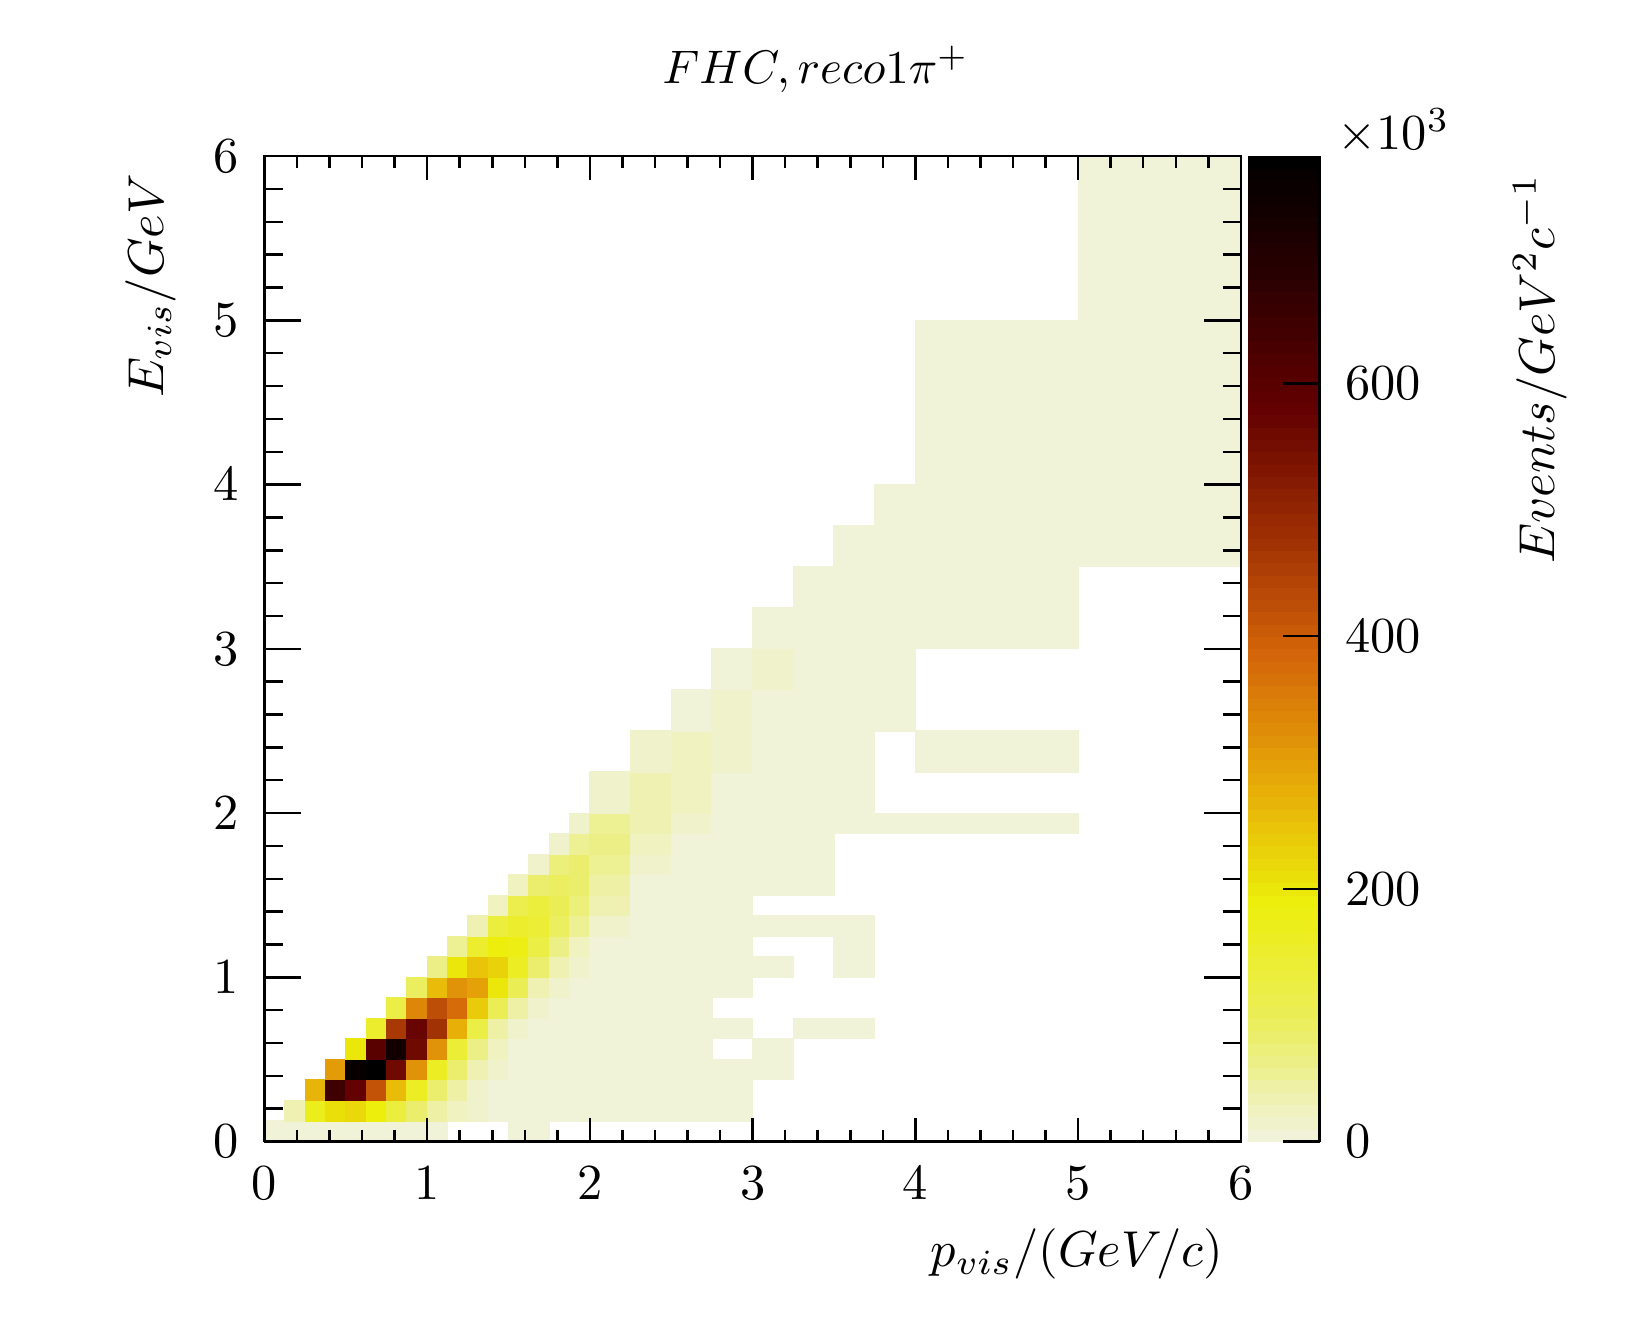
\begin{tikzpicture}
\pgfdeclareplotmark{cross} {
\pgfpathmoveto{\pgfpoint{-0.3\pgfplotmarksize}{\pgfplotmarksize}}
\pgfpathlineto{\pgfpoint{+0.3\pgfplotmarksize}{\pgfplotmarksize}}
\pgfpathlineto{\pgfpoint{+0.3\pgfplotmarksize}{0.3\pgfplotmarksize}}
\pgfpathlineto{\pgfpoint{+1\pgfplotmarksize}{0.3\pgfplotmarksize}}
\pgfpathlineto{\pgfpoint{+1\pgfplotmarksize}{-0.3\pgfplotmarksize}}
\pgfpathlineto{\pgfpoint{+0.3\pgfplotmarksize}{-0.3\pgfplotmarksize}}
\pgfpathlineto{\pgfpoint{+0.3\pgfplotmarksize}{-1.\pgfplotmarksize}}
\pgfpathlineto{\pgfpoint{-0.3\pgfplotmarksize}{-1.\pgfplotmarksize}}
\pgfpathlineto{\pgfpoint{-0.3\pgfplotmarksize}{-0.3\pgfplotmarksize}}
\pgfpathlineto{\pgfpoint{-1.\pgfplotmarksize}{-0.3\pgfplotmarksize}}
\pgfpathlineto{\pgfpoint{-1.\pgfplotmarksize}{0.3\pgfplotmarksize}}
\pgfpathlineto{\pgfpoint{-0.3\pgfplotmarksize}{0.3\pgfplotmarksize}}
\pgfpathclose
\pgfusepathqstroke
}
\pgfdeclareplotmark{cross*} {
\pgfpathmoveto{\pgfpoint{-0.3\pgfplotmarksize}{\pgfplotmarksize}}
\pgfpathlineto{\pgfpoint{+0.3\pgfplotmarksize}{\pgfplotmarksize}}
\pgfpathlineto{\pgfpoint{+0.3\pgfplotmarksize}{0.3\pgfplotmarksize}}
\pgfpathlineto{\pgfpoint{+1\pgfplotmarksize}{0.3\pgfplotmarksize}}
\pgfpathlineto{\pgfpoint{+1\pgfplotmarksize}{-0.3\pgfplotmarksize}}
\pgfpathlineto{\pgfpoint{+0.3\pgfplotmarksize}{-0.3\pgfplotmarksize}}
\pgfpathlineto{\pgfpoint{+0.3\pgfplotmarksize}{-1.\pgfplotmarksize}}
\pgfpathlineto{\pgfpoint{-0.3\pgfplotmarksize}{-1.\pgfplotmarksize}}
\pgfpathlineto{\pgfpoint{-0.3\pgfplotmarksize}{-0.3\pgfplotmarksize}}
\pgfpathlineto{\pgfpoint{-1.\pgfplotmarksize}{-0.3\pgfplotmarksize}}
\pgfpathlineto{\pgfpoint{-1.\pgfplotmarksize}{0.3\pgfplotmarksize}}
\pgfpathlineto{\pgfpoint{-0.3\pgfplotmarksize}{0.3\pgfplotmarksize}}
\pgfpathclose
\pgfusepathqfillstroke
}
\pgfdeclareplotmark{newstar} {
\pgfpathmoveto{\pgfqpoint{0pt}{\pgfplotmarksize}}
\pgfpathlineto{\pgfqpointpolar{44}{0.5\pgfplotmarksize}}
\pgfpathlineto{\pgfqpointpolar{18}{\pgfplotmarksize}}
\pgfpathlineto{\pgfqpointpolar{-20}{0.5\pgfplotmarksize}}
\pgfpathlineto{\pgfqpointpolar{-54}{\pgfplotmarksize}}
\pgfpathlineto{\pgfqpointpolar{-90}{0.5\pgfplotmarksize}}
\pgfpathlineto{\pgfqpointpolar{234}{\pgfplotmarksize}}
\pgfpathlineto{\pgfqpointpolar{198}{0.5\pgfplotmarksize}}
\pgfpathlineto{\pgfqpointpolar{162}{\pgfplotmarksize}}
\pgfpathlineto{\pgfqpointpolar{134}{0.5\pgfplotmarksize}}
\pgfpathclose
\pgfusepathqstroke
}
\pgfdeclareplotmark{newstar*} {
\pgfpathmoveto{\pgfqpoint{0pt}{\pgfplotmarksize}}
\pgfpathlineto{\pgfqpointpolar{44}{0.5\pgfplotmarksize}}
\pgfpathlineto{\pgfqpointpolar{18}{\pgfplotmarksize}}
\pgfpathlineto{\pgfqpointpolar{-20}{0.5\pgfplotmarksize}}
\pgfpathlineto{\pgfqpointpolar{-54}{\pgfplotmarksize}}
\pgfpathlineto{\pgfqpointpolar{-90}{0.5\pgfplotmarksize}}
\pgfpathlineto{\pgfqpointpolar{234}{\pgfplotmarksize}}
\pgfpathlineto{\pgfqpointpolar{198}{0.5\pgfplotmarksize}}
\pgfpathlineto{\pgfqpointpolar{162}{\pgfplotmarksize}}
\pgfpathlineto{\pgfqpointpolar{134}{0.5\pgfplotmarksize}}
\pgfpathclose
\pgfusepathqfillstroke
}
\definecolor{c}{rgb}{1,1,1};
\draw [color=c, fill=c] (0,0) rectangle (20,16.2517);
\draw [color=c, fill=c] (3,2.11272) rectangle (15.4,14.6265);
\definecolor{c}{rgb}{0,0,0};
\draw [c,line width=0.9] (3,2.11272) -- (3,14.6265) -- (15.4,14.6265) -- (15.4,2.11272) -- (3,2.11272);
\definecolor{c}{rgb}{1,1,1};
\draw [color=c, fill=c] (3,2.11272) rectangle (15.4,14.6265);
\definecolor{c}{rgb}{0,0,0};
\draw [c,line width=0.9] (3,2.11272) -- (3,14.6265) -- (15.4,14.6265) -- (15.4,2.11272) -- (3,2.11272);
\definecolor{c}{rgb}{0.945984,0.951044,0.850727};
\draw [color=c, fill=c] (3,2.11272) rectangle (3.25833,2.37343);
\draw [color=c, fill=c] (3.25833,2.11272) rectangle (3.51667,2.37343);
\draw [color=c, fill=c] (3.51667,2.11272) rectangle (3.775,2.37343);
\draw [color=c, fill=c] (3.775,2.11272) rectangle (4.03333,2.37343);
\draw [color=c, fill=c] (4.03333,2.11272) rectangle (4.29167,2.37343);
\draw [color=c, fill=c] (4.29167,2.11272) rectangle (4.55,2.37343);
\draw [color=c, fill=c] (4.55,2.11272) rectangle (4.80833,2.37343);
\draw [color=c, fill=c] (4.80833,2.11272) rectangle (5.06667,2.37343);
\draw [color=c, fill=c] (5.06667,2.11272) rectangle (5.325,2.37343);
\draw [color=c, fill=c] (6.1,2.11272) rectangle (6.35833,2.37343);
\draw [color=c, fill=c] (6.35833,2.11272) rectangle (6.61667,2.37343);
\definecolor{c}{rgb}{0.936875,0.945351,0.697027};
\draw [color=c, fill=c] (3.25833,2.37343) rectangle (3.51667,2.63413);
\definecolor{c}{rgb}{0.927206,0.933333,0.104902};
\draw [color=c, fill=c] (3.51667,2.37343) rectangle (3.775,2.63413);
\definecolor{c}{rgb}{0.923407,0.873284,0.0405637};
\draw [color=c, fill=c] (3.775,2.37343) rectangle (4.03333,2.63413);
\definecolor{c}{rgb}{0.920833,0.847549,0.0394608};
\draw [color=c, fill=c] (4.03333,2.37343) rectangle (4.29167,2.63413);
\definecolor{c}{rgb}{0.929412,0.933333,0.0431373};
\draw [color=c, fill=c] (4.29167,2.37343) rectangle (4.55,2.63413);
\definecolor{c}{rgb}{0.922426,0.933333,0.238725};
\draw [color=c, fill=c] (4.55,2.37343) rectangle (4.80833,2.63413);
\definecolor{c}{rgb}{0.920683,0.935231,0.423782};
\draw [color=c, fill=c] (4.80833,2.37343) rectangle (5.06667,2.63413);
\definecolor{c}{rgb}{0.933839,0.943453,0.645794};
\draw [color=c, fill=c] (5.06667,2.37343) rectangle (5.325,2.63413);
\definecolor{c}{rgb}{0.939911,0.947249,0.748261};
\draw [color=c, fill=c] (5.325,2.37343) rectangle (5.58333,2.63413);
\definecolor{c}{rgb}{0.942948,0.949146,0.799494};
\draw [color=c, fill=c] (5.58333,2.37343) rectangle (5.84167,2.63413);
\definecolor{c}{rgb}{0.945984,0.951044,0.850727};
\draw [color=c, fill=c] (5.84167,2.37343) rectangle (6.1,2.63413);
\draw [color=c, fill=c] (6.1,2.37343) rectangle (6.35833,2.63413);
\draw [color=c, fill=c] (6.35833,2.37343) rectangle (6.61667,2.63413);
\draw [color=c, fill=c] (6.61667,2.37343) rectangle (6.875,2.63413);
\draw [color=c, fill=c] (6.875,2.37343) rectangle (7.13333,2.63413);
\draw [color=c, fill=c] (7.13333,2.37343) rectangle (7.65,2.63413);
\draw [color=c, fill=c] (7.65,2.37343) rectangle (8.16667,2.63413);
\draw [color=c, fill=c] (8.16667,2.37343) rectangle (8.68333,2.63413);
\draw [color=c, fill=c] (8.68333,2.37343) rectangle (9.2,2.63413);
\definecolor{c}{rgb}{0.907108,0.710294,0.0335784};
\draw [color=c, fill=c] (3.51667,2.63413) rectangle (3.775,2.89484);
\definecolor{c}{rgb}{0.242647,0,0.00392157};
\draw [color=c, fill=c] (3.775,2.63413) rectangle (4.03333,2.89484);
\definecolor{c}{rgb}{0.388235,0,0.00392157};
\draw [color=c, fill=c] (4.03333,2.63413) rectangle (4.29167,2.89484);
\definecolor{c}{rgb}{0.762745,0.327451,0.0279412};
\draw [color=c, fill=c] (4.29167,2.63413) rectangle (4.55,2.89484);
\definecolor{c}{rgb}{0.909681,0.736029,0.0346814};
\draw [color=c, fill=c] (4.55,2.63413) rectangle (4.80833,2.89484);
\definecolor{c}{rgb}{0.926103,0.933333,0.135784};
\draw [color=c, fill=c] (4.80833,2.63413) rectangle (5.06667,2.89484);
\definecolor{c}{rgb}{0.920683,0.935231,0.423782};
\draw [color=c, fill=c] (5.06667,2.63413) rectangle (5.325,2.89484);
\definecolor{c}{rgb}{0.933839,0.943453,0.645794};
\draw [color=c, fill=c] (5.325,2.63413) rectangle (5.58333,2.89484);
\definecolor{c}{rgb}{0.942948,0.949146,0.799494};
\draw [color=c, fill=c] (5.58333,2.63413) rectangle (5.84167,2.89484);
\definecolor{c}{rgb}{0.945984,0.951044,0.850727};
\draw [color=c, fill=c] (5.84167,2.63413) rectangle (6.1,2.89484);
\draw [color=c, fill=c] (6.1,2.63413) rectangle (6.35833,2.89484);
\draw [color=c, fill=c] (6.35833,2.63413) rectangle (6.61667,2.89484);
\draw [color=c, fill=c] (6.61667,2.63413) rectangle (6.875,2.89484);
\draw [color=c, fill=c] (6.875,2.63413) rectangle (7.13333,2.89484);
\draw [color=c, fill=c] (7.13333,2.63413) rectangle (7.65,2.89484);
\draw [color=c, fill=c] (7.65,2.63413) rectangle (8.16667,2.89484);
\draw [color=c, fill=c] (8.16667,2.63413) rectangle (8.68333,2.89484);
\draw [color=c, fill=c] (8.68333,2.63413) rectangle (9.2,2.89484);
\definecolor{c}{rgb}{0.888726,0.609559,0.0321078};
\draw [color=c, fill=c] (3.775,2.89484) rectangle (4.03333,3.15554);
\definecolor{c}{rgb}{0.0220588,0,0.000490196};
\draw [color=c, fill=c] (4.03333,2.89484) rectangle (4.29167,3.15554);
\definecolor{c}{rgb}{0.00551471,0,0.000122549};
\draw [color=c, fill=c] (4.29167,2.89484) rectangle (4.55,3.15554);
\definecolor{c}{rgb}{0.437132,0.0386029,0.00563726};
\draw [color=c, fill=c] (4.55,2.89484) rectangle (4.80833,3.15554);
\definecolor{c}{rgb}{0.879902,0.576716,0.032598};
\draw [color=c, fill=c] (4.80833,2.89484) rectangle (5.06667,3.15554);
\definecolor{c}{rgb}{0.926103,0.933333,0.135784};
\draw [color=c, fill=c] (5.06667,2.89484) rectangle (5.325,3.15554);
\definecolor{c}{rgb}{0.920683,0.935231,0.423782};
\draw [color=c, fill=c] (5.325,2.89484) rectangle (5.58333,3.15554);
\definecolor{c}{rgb}{0.936875,0.945351,0.697027};
\draw [color=c, fill=c] (5.58333,2.89484) rectangle (5.84167,3.15554);
\definecolor{c}{rgb}{0.942948,0.949146,0.799494};
\draw [color=c, fill=c] (5.84167,2.89484) rectangle (6.1,3.15554);
\definecolor{c}{rgb}{0.945984,0.951044,0.850727};
\draw [color=c, fill=c] (6.1,2.89484) rectangle (6.35833,3.15554);
\draw [color=c, fill=c] (6.35833,2.89484) rectangle (6.61667,3.15554);
\draw [color=c, fill=c] (6.61667,2.89484) rectangle (6.875,3.15554);
\draw [color=c, fill=c] (6.875,2.89484) rectangle (7.13333,3.15554);
\draw [color=c, fill=c] (7.13333,2.89484) rectangle (7.65,3.15554);
\draw [color=c, fill=c] (7.65,2.89484) rectangle (8.16667,3.15554);
\draw [color=c, fill=c] (8.16667,2.89484) rectangle (8.68333,3.15554);
\draw [color=c, fill=c] (8.68333,2.89484) rectangle (9.2,3.15554);
\draw [color=c, fill=c] (9.2,2.89484) rectangle (9.71667,3.15554);
\definecolor{c}{rgb}{0.926838,0.907598,0.0420343};
\draw [color=c, fill=c] (4.03333,3.15554) rectangle (4.29167,3.41624);
\definecolor{c}{rgb}{0.348529,0,0.00392157};
\draw [color=c, fill=c] (4.29167,3.15554) rectangle (4.55,3.41624);
\definecolor{c}{rgb}{0.0716912,0,0.00159314};
\draw [color=c, fill=c] (4.55,3.15554) rectangle (4.80833,3.41624);
\definecolor{c}{rgb}{0.437132,0.0386029,0.00563726};
\draw [color=c, fill=c] (4.80833,3.15554) rectangle (5.06667,3.41624);
\definecolor{c}{rgb}{0.879902,0.576716,0.032598};
\draw [color=c, fill=c] (5.06667,3.15554) rectangle (5.325,3.41624);
\definecolor{c}{rgb}{0.923529,0.933333,0.207843};
\draw [color=c, fill=c] (5.325,3.15554) rectangle (5.58333,3.41624);
\definecolor{c}{rgb}{0.926755,0.939026,0.526249};
\draw [color=c, fill=c] (5.58333,3.15554) rectangle (5.84167,3.41624);
\definecolor{c}{rgb}{0.939911,0.947249,0.748261};
\draw [color=c, fill=c] (5.84167,3.15554) rectangle (6.1,3.41624);
\definecolor{c}{rgb}{0.945984,0.951044,0.850727};
\draw [color=c, fill=c] (6.1,3.15554) rectangle (6.35833,3.41624);
\draw [color=c, fill=c] (6.35833,3.15554) rectangle (6.61667,3.41624);
\draw [color=c, fill=c] (6.61667,3.15554) rectangle (6.875,3.41624);
\draw [color=c, fill=c] (6.875,3.15554) rectangle (7.13333,3.41624);
\draw [color=c, fill=c] (7.13333,3.15554) rectangle (7.65,3.41624);
\draw [color=c, fill=c] (7.65,3.15554) rectangle (8.16667,3.41624);
\draw [color=c, fill=c] (8.16667,3.15554) rectangle (8.68333,3.41624);
\draw [color=c, fill=c] (9.2,3.15554) rectangle (9.71667,3.41624);
\definecolor{c}{rgb}{0.924632,0.933333,0.176961};
\draw [color=c, fill=c] (4.29167,3.41624) rectangle (4.55,3.67695);
\definecolor{c}{rgb}{0.659804,0.22451,0.0169118};
\draw [color=c, fill=c] (4.55,3.41624) rectangle (4.80833,3.67695);
\definecolor{c}{rgb}{0.409191,0.0165441,0.00465686};
\draw [color=c, fill=c] (4.80833,3.41624) rectangle (5.06667,3.67695);
\definecolor{c}{rgb}{0.632353,0.197059,0.0139706};
\draw [color=c, fill=c] (5.06667,3.41624) rectangle (5.325,3.67695);
\definecolor{c}{rgb}{0.904534,0.684559,0.0324755};
\draw [color=c, fill=c] (5.325,3.41624) rectangle (5.58333,3.67695);
\definecolor{c}{rgb}{0.921324,0.933333,0.269608};
\draw [color=c, fill=c] (5.58333,3.41624) rectangle (5.84167,3.67695);
\definecolor{c}{rgb}{0.933839,0.943453,0.645794};
\draw [color=c, fill=c] (5.84167,3.41624) rectangle (6.1,3.67695);
\definecolor{c}{rgb}{0.942948,0.949146,0.799494};
\draw [color=c, fill=c] (6.1,3.41624) rectangle (6.35833,3.67695);
\definecolor{c}{rgb}{0.945984,0.951044,0.850727};
\draw [color=c, fill=c] (6.35833,3.41624) rectangle (6.61667,3.67695);
\draw [color=c, fill=c] (6.61667,3.41624) rectangle (6.875,3.67695);
\draw [color=c, fill=c] (6.875,3.41624) rectangle (7.13333,3.67695);
\draw [color=c, fill=c] (7.13333,3.41624) rectangle (7.65,3.67695);
\draw [color=c, fill=c] (7.65,3.41624) rectangle (8.16667,3.67695);
\draw [color=c, fill=c] (8.16667,3.41624) rectangle (8.68333,3.67695);
\draw [color=c, fill=c] (8.68333,3.41624) rectangle (9.2,3.67695);
\draw [color=c, fill=c] (9.71667,3.41624) rectangle (10.2333,3.67695);
\draw [color=c, fill=c] (10.2333,3.41624) rectangle (10.75,3.67695);
\definecolor{c}{rgb}{0.921324,0.933333,0.269608};
\draw [color=c, fill=c] (4.55,3.67695) rectangle (4.80833,3.93765);
\definecolor{c}{rgb}{0.866667,0.527451,0.0333333};
\draw [color=c, fill=c] (4.80833,3.67695) rectangle (5.06667,3.93765);
\definecolor{c}{rgb}{0.742157,0.306863,0.0257353};
\draw [color=c, fill=c] (5.06667,3.67695) rectangle (5.325,3.93765);
\definecolor{c}{rgb}{0.83799,0.420711,0.0349265};
\draw [color=c, fill=c] (5.325,3.67695) rectangle (5.58333,3.93765);
\definecolor{c}{rgb}{0.915686,0.796078,0.0372549};
\draw [color=c, fill=c] (5.58333,3.67695) rectangle (5.84167,3.93765);
\definecolor{c}{rgb}{0.919118,0.933333,0.331373};
\draw [color=c, fill=c] (5.84167,3.67695) rectangle (6.1,3.93765);
\definecolor{c}{rgb}{0.933839,0.943453,0.645794};
\draw [color=c, fill=c] (6.1,3.67695) rectangle (6.35833,3.93765);
\definecolor{c}{rgb}{0.942948,0.949146,0.799494};
\draw [color=c, fill=c] (6.35833,3.67695) rectangle (6.61667,3.93765);
\definecolor{c}{rgb}{0.945984,0.951044,0.850727};
\draw [color=c, fill=c] (6.61667,3.67695) rectangle (6.875,3.93765);
\draw [color=c, fill=c] (6.875,3.67695) rectangle (7.13333,3.93765);
\draw [color=c, fill=c] (7.13333,3.67695) rectangle (7.65,3.93765);
\draw [color=c, fill=c] (7.65,3.67695) rectangle (8.16667,3.93765);
\draw [color=c, fill=c] (8.16667,3.67695) rectangle (8.68333,3.93765);
\definecolor{c}{rgb}{0.917647,0.933333,0.372549};
\draw [color=c, fill=c] (4.80833,3.93765) rectangle (5.06667,4.19836);
\definecolor{c}{rgb}{0.909681,0.736029,0.0346814};
\draw [color=c, fill=c] (5.06667,3.93765) rectangle (5.325,4.19836);
\definecolor{c}{rgb}{0.879902,0.576716,0.032598};
\draw [color=c, fill=c] (5.325,3.93765) rectangle (5.58333,4.19836);
\definecolor{c}{rgb}{0.895343,0.634191,0.0317402};
\draw [color=c, fill=c] (5.58333,3.93765) rectangle (5.84167,4.19836);
\definecolor{c}{rgb}{0.926838,0.907598,0.0420343};
\draw [color=c, fill=c] (5.84167,3.93765) rectangle (6.1,4.19836);
\definecolor{c}{rgb}{0.919118,0.933333,0.331373};
\draw [color=c, fill=c] (6.1,3.93765) rectangle (6.35833,4.19836);
\definecolor{c}{rgb}{0.936875,0.945351,0.697027};
\draw [color=c, fill=c] (6.35833,3.93765) rectangle (6.61667,4.19836);
\definecolor{c}{rgb}{0.942948,0.949146,0.799494};
\draw [color=c, fill=c] (6.61667,3.93765) rectangle (6.875,4.19836);
\definecolor{c}{rgb}{0.945984,0.951044,0.850727};
\draw [color=c, fill=c] (6.875,3.93765) rectangle (7.13333,4.19836);
\draw [color=c, fill=c] (7.13333,3.93765) rectangle (7.65,4.19836);
\draw [color=c, fill=c] (7.65,3.93765) rectangle (8.16667,4.19836);
\draw [color=c, fill=c] (8.16667,3.93765) rectangle (8.68333,4.19836);
\draw [color=c, fill=c] (8.68333,3.93765) rectangle (9.2,4.19836);
\definecolor{c}{rgb}{0.926755,0.939026,0.526249};
\draw [color=c, fill=c] (5.06667,4.19836) rectangle (5.325,4.45906);
\definecolor{c}{rgb}{0.926838,0.907598,0.0420343};
\draw [color=c, fill=c] (5.325,4.19836) rectangle (5.58333,4.45906);
\definecolor{c}{rgb}{0.913113,0.770343,0.036152};
\draw [color=c, fill=c] (5.58333,4.19836) rectangle (5.84167,4.45906);
\definecolor{c}{rgb}{0.91826,0.821814,0.0383578};
\draw [color=c, fill=c] (5.84167,4.19836) rectangle (6.1,4.45906);
\definecolor{c}{rgb}{0.926103,0.933333,0.135784};
\draw [color=c, fill=c] (6.1,4.19836) rectangle (6.35833,4.45906);
\definecolor{c}{rgb}{0.920683,0.935231,0.423782};
\draw [color=c, fill=c] (6.35833,4.19836) rectangle (6.61667,4.45906);
\definecolor{c}{rgb}{0.936875,0.945351,0.697027};
\draw [color=c, fill=c] (6.61667,4.19836) rectangle (6.875,4.45906);
\definecolor{c}{rgb}{0.942948,0.949146,0.799494};
\draw [color=c, fill=c] (6.875,4.19836) rectangle (7.13333,4.45906);
\definecolor{c}{rgb}{0.945984,0.951044,0.850727};
\draw [color=c, fill=c] (7.13333,4.19836) rectangle (7.65,4.45906);
\draw [color=c, fill=c] (7.65,4.19836) rectangle (8.16667,4.45906);
\draw [color=c, fill=c] (8.16667,4.19836) rectangle (8.68333,4.45906);
\draw [color=c, fill=c] (8.68333,4.19836) rectangle (9.2,4.45906);
\draw [color=c, fill=c] (9.2,4.19836) rectangle (9.71667,4.45906);
\draw [color=c, fill=c] (10.2333,4.19836) rectangle (10.75,4.45906);
\definecolor{c}{rgb}{0.929791,0.940923,0.577483};
\draw [color=c, fill=c] (5.325,4.45906) rectangle (5.58333,4.71977);
\definecolor{c}{rgb}{0.924632,0.933333,0.176961};
\draw [color=c, fill=c] (5.58333,4.45906) rectangle (5.84167,4.71977);
\definecolor{c}{rgb}{0.929412,0.933333,0.0431373};
\draw [color=c, fill=c] (5.84167,4.45906) rectangle (6.1,4.71977);
\definecolor{c}{rgb}{0.928309,0.933333,0.0740196};
\draw [color=c, fill=c] (6.1,4.45906) rectangle (6.35833,4.71977);
\definecolor{c}{rgb}{0.921324,0.933333,0.269608};
\draw [color=c, fill=c] (6.35833,4.45906) rectangle (6.61667,4.71977);
\definecolor{c}{rgb}{0.926755,0.939026,0.526249};
\draw [color=c, fill=c] (6.61667,4.45906) rectangle (6.875,4.71977);
\definecolor{c}{rgb}{0.939911,0.947249,0.748261};
\draw [color=c, fill=c] (6.875,4.45906) rectangle (7.13333,4.71977);
\definecolor{c}{rgb}{0.945984,0.951044,0.850727};
\draw [color=c, fill=c] (7.13333,4.45906) rectangle (7.65,4.71977);
\draw [color=c, fill=c] (7.65,4.45906) rectangle (8.16667,4.71977);
\draw [color=c, fill=c] (8.16667,4.45906) rectangle (8.68333,4.71977);
\draw [color=c, fill=c] (8.68333,4.45906) rectangle (9.2,4.71977);
\draw [color=c, fill=c] (10.2333,4.45906) rectangle (10.75,4.71977);
\definecolor{c}{rgb}{0.936875,0.945351,0.697027};
\draw [color=c, fill=c] (5.58333,4.71977) rectangle (5.84167,4.98047);
\definecolor{c}{rgb}{0.922426,0.933333,0.238725};
\draw [color=c, fill=c] (5.84167,4.71977) rectangle (6.1,4.98047);
\definecolor{c}{rgb}{0.924632,0.933333,0.176961};
\draw [color=c, fill=c] (6.1,4.71977) rectangle (6.35833,4.98047);
\definecolor{c}{rgb}{0.923529,0.933333,0.207843};
\draw [color=c, fill=c] (6.35833,4.71977) rectangle (6.61667,4.98047);
\definecolor{c}{rgb}{0.917647,0.933333,0.372549};
\draw [color=c, fill=c] (6.61667,4.71977) rectangle (6.875,4.98047);
\definecolor{c}{rgb}{0.929791,0.940923,0.577483};
\draw [color=c, fill=c] (6.875,4.71977) rectangle (7.13333,4.98047);
\definecolor{c}{rgb}{0.942948,0.949146,0.799494};
\draw [color=c, fill=c] (7.13333,4.71977) rectangle (7.65,4.98047);
\definecolor{c}{rgb}{0.945984,0.951044,0.850727};
\draw [color=c, fill=c] (7.65,4.71977) rectangle (8.16667,4.98047);
\draw [color=c, fill=c] (8.16667,4.71977) rectangle (8.68333,4.98047);
\draw [color=c, fill=c] (8.68333,4.71977) rectangle (9.2,4.98047);
\draw [color=c, fill=c] (9.2,4.71977) rectangle (9.71667,4.98047);
\draw [color=c, fill=c] (9.71667,4.71977) rectangle (10.2333,4.98047);
\draw [color=c, fill=c] (10.2333,4.71977) rectangle (10.75,4.98047);
\definecolor{c}{rgb}{0.939911,0.947249,0.748261};
\draw [color=c, fill=c] (5.84167,4.98047) rectangle (6.1,5.24118);
\definecolor{c}{rgb}{0.920221,0.933333,0.30049};
\draw [color=c, fill=c] (6.1,4.98047) rectangle (6.35833,5.24118);
\definecolor{c}{rgb}{0.922426,0.933333,0.238725};
\draw [color=c, fill=c] (6.35833,4.98047) rectangle (6.61667,5.24118);
\definecolor{c}{rgb}{0.919118,0.933333,0.331373};
\draw [color=c, fill=c] (6.61667,4.98047) rectangle (6.875,5.24118);
\definecolor{c}{rgb}{0.923719,0.937128,0.475016};
\draw [color=c, fill=c] (6.875,4.98047) rectangle (7.13333,5.24118);
\definecolor{c}{rgb}{0.936875,0.945351,0.697027};
\draw [color=c, fill=c] (7.13333,4.98047) rectangle (7.65,5.24118);
\definecolor{c}{rgb}{0.945984,0.951044,0.850727};
\draw [color=c, fill=c] (7.65,4.98047) rectangle (8.16667,5.24118);
\draw [color=c, fill=c] (8.16667,4.98047) rectangle (8.68333,5.24118);
\draw [color=c, fill=c] (8.68333,4.98047) rectangle (9.2,5.24118);
\definecolor{c}{rgb}{0.939911,0.947249,0.748261};
\draw [color=c, fill=c] (6.1,5.24118) rectangle (6.35833,5.50188);
\definecolor{c}{rgb}{0.920683,0.935231,0.423782};
\draw [color=c, fill=c] (6.35833,5.24118) rectangle (6.61667,5.50188);
\definecolor{c}{rgb}{0.917647,0.933333,0.372549};
\draw [color=c, fill=c] (6.61667,5.24118) rectangle (6.875,5.50188);
\definecolor{c}{rgb}{0.920683,0.935231,0.423782};
\draw [color=c, fill=c] (6.875,5.24118) rectangle (7.13333,5.50188);
\definecolor{c}{rgb}{0.933839,0.943453,0.645794};
\draw [color=c, fill=c] (7.13333,5.24118) rectangle (7.65,5.50188);
\definecolor{c}{rgb}{0.945984,0.951044,0.850727};
\draw [color=c, fill=c] (7.65,5.24118) rectangle (8.16667,5.50188);
\draw [color=c, fill=c] (8.16667,5.24118) rectangle (8.68333,5.50188);
\draw [color=c, fill=c] (8.68333,5.24118) rectangle (9.2,5.50188);
\draw [color=c, fill=c] (9.2,5.24118) rectangle (9.71667,5.50188);
\draw [color=c, fill=c] (9.71667,5.24118) rectangle (10.2333,5.50188);
\definecolor{c}{rgb}{0.942948,0.949146,0.799494};
\draw [color=c, fill=c] (6.35833,5.50188) rectangle (6.61667,5.76259);
\definecolor{c}{rgb}{0.923719,0.937128,0.475016};
\draw [color=c, fill=c] (6.61667,5.50188) rectangle (6.875,5.76259);
\definecolor{c}{rgb}{0.920683,0.935231,0.423782};
\draw [color=c, fill=c] (6.875,5.50188) rectangle (7.13333,5.76259);
\definecolor{c}{rgb}{0.929791,0.940923,0.577483};
\draw [color=c, fill=c] (7.13333,5.50188) rectangle (7.65,5.76259);
\definecolor{c}{rgb}{0.942948,0.949146,0.799494};
\draw [color=c, fill=c] (7.65,5.50188) rectangle (8.16667,5.76259);
\definecolor{c}{rgb}{0.945984,0.951044,0.850727};
\draw [color=c, fill=c] (8.16667,5.50188) rectangle (8.68333,5.76259);
\draw [color=c, fill=c] (8.68333,5.50188) rectangle (9.2,5.76259);
\draw [color=c, fill=c] (9.2,5.50188) rectangle (9.71667,5.76259);
\draw [color=c, fill=c] (9.71667,5.50188) rectangle (10.2333,5.76259);
\definecolor{c}{rgb}{0.942948,0.949146,0.799494};
\draw [color=c, fill=c] (6.61667,5.76259) rectangle (6.875,6.02329);
\definecolor{c}{rgb}{0.929791,0.940923,0.577483};
\draw [color=c, fill=c] (6.875,5.76259) rectangle (7.13333,6.02329);
\definecolor{c}{rgb}{0.926755,0.939026,0.526249};
\draw [color=c, fill=c] (7.13333,5.76259) rectangle (7.65,6.02329);
\definecolor{c}{rgb}{0.939911,0.947249,0.748261};
\draw [color=c, fill=c] (7.65,5.76259) rectangle (8.16667,6.02329);
\definecolor{c}{rgb}{0.945984,0.951044,0.850727};
\draw [color=c, fill=c] (8.16667,5.76259) rectangle (8.68333,6.02329);
\draw [color=c, fill=c] (8.68333,5.76259) rectangle (9.2,6.02329);
\draw [color=c, fill=c] (9.2,5.76259) rectangle (9.71667,6.02329);
\draw [color=c, fill=c] (9.71667,5.76259) rectangle (10.2333,6.02329);
\definecolor{c}{rgb}{0.942948,0.949146,0.799494};
\draw [color=c, fill=c] (6.875,6.02329) rectangle (7.13333,6.28399);
\definecolor{c}{rgb}{0.929791,0.940923,0.577483};
\draw [color=c, fill=c] (7.13333,6.02329) rectangle (7.65,6.28399);
\definecolor{c}{rgb}{0.936875,0.945351,0.697027};
\draw [color=c, fill=c] (7.65,6.02329) rectangle (8.16667,6.28399);
\definecolor{c}{rgb}{0.942948,0.949146,0.799494};
\draw [color=c, fill=c] (8.16667,6.02329) rectangle (8.68333,6.28399);
\definecolor{c}{rgb}{0.945984,0.951044,0.850727};
\draw [color=c, fill=c] (8.68333,6.02329) rectangle (9.2,6.28399);
\draw [color=c, fill=c] (9.2,6.02329) rectangle (9.71667,6.28399);
\draw [color=c, fill=c] (9.71667,6.02329) rectangle (10.2333,6.28399);
\draw [color=c, fill=c] (10.2333,6.02329) rectangle (10.75,6.28399);
\draw [color=c, fill=c] (10.75,6.02329) rectangle (11.2667,6.28399);
\draw [color=c, fill=c] (11.2667,6.02329) rectangle (13.3333,6.28399);
\definecolor{c}{rgb}{0.942948,0.949146,0.799494};
\draw [color=c, fill=c] (7.13333,6.28399) rectangle (7.65,6.8054);
\definecolor{c}{rgb}{0.936875,0.945351,0.697027};
\draw [color=c, fill=c] (7.65,6.28399) rectangle (8.16667,6.8054);
\definecolor{c}{rgb}{0.939911,0.947249,0.748261};
\draw [color=c, fill=c] (8.16667,6.28399) rectangle (8.68333,6.8054);
\definecolor{c}{rgb}{0.945984,0.951044,0.850727};
\draw [color=c, fill=c] (8.68333,6.28399) rectangle (9.2,6.8054);
\draw [color=c, fill=c] (9.2,6.28399) rectangle (9.71667,6.8054);
\draw [color=c, fill=c] (9.71667,6.28399) rectangle (10.2333,6.8054);
\draw [color=c, fill=c] (10.2333,6.28399) rectangle (10.75,6.8054);
\definecolor{c}{rgb}{0.942948,0.949146,0.799494};
\draw [color=c, fill=c] (7.65,6.8054) rectangle (8.16667,7.32681);
\definecolor{c}{rgb}{0.939911,0.947249,0.748261};
\draw [color=c, fill=c] (8.16667,6.8054) rectangle (8.68333,7.32681);
\definecolor{c}{rgb}{0.942948,0.949146,0.799494};
\draw [color=c, fill=c] (8.68333,6.8054) rectangle (9.2,7.32681);
\definecolor{c}{rgb}{0.945984,0.951044,0.850727};
\draw [color=c, fill=c] (9.2,6.8054) rectangle (9.71667,7.32681);
\draw [color=c, fill=c] (9.71667,6.8054) rectangle (10.2333,7.32681);
\draw [color=c, fill=c] (10.2333,6.8054) rectangle (10.75,7.32681);
\draw [color=c, fill=c] (11.2667,6.8054) rectangle (13.3333,7.32681);
\draw [color=c, fill=c] (8.16667,7.32681) rectangle (8.68333,7.84822);
\definecolor{c}{rgb}{0.942948,0.949146,0.799494};
\draw [color=c, fill=c] (8.68333,7.32681) rectangle (9.2,7.84822);
\definecolor{c}{rgb}{0.945984,0.951044,0.850727};
\draw [color=c, fill=c] (9.2,7.32681) rectangle (9.71667,7.84822);
\draw [color=c, fill=c] (9.71667,7.32681) rectangle (10.2333,7.84822);
\draw [color=c, fill=c] (10.2333,7.32681) rectangle (10.75,7.84822);
\draw [color=c, fill=c] (10.75,7.32681) rectangle (11.2667,7.84822);
\draw [color=c, fill=c] (8.68333,7.84822) rectangle (9.2,8.36963);
\definecolor{c}{rgb}{0.942948,0.949146,0.799494};
\draw [color=c, fill=c] (9.2,7.84822) rectangle (9.71667,8.36963);
\definecolor{c}{rgb}{0.945984,0.951044,0.850727};
\draw [color=c, fill=c] (9.71667,7.84822) rectangle (10.2333,8.36963);
\draw [color=c, fill=c] (10.2333,7.84822) rectangle (10.75,8.36963);
\draw [color=c, fill=c] (10.75,7.84822) rectangle (11.2667,8.36963);
\draw [color=c, fill=c] (9.2,8.36963) rectangle (9.71667,8.89104);
\draw [color=c, fill=c] (9.71667,8.36963) rectangle (10.2333,8.89104);
\draw [color=c, fill=c] (10.2333,8.36963) rectangle (10.75,8.89104);
\draw [color=c, fill=c] (10.75,8.36963) rectangle (11.2667,8.89104);
\draw [color=c, fill=c] (11.2667,8.36963) rectangle (13.3333,8.89104);
\draw [color=c, fill=c] (9.71667,8.89104) rectangle (10.2333,9.41245);
\draw [color=c, fill=c] (10.2333,8.89104) rectangle (10.75,9.41245);
\draw [color=c, fill=c] (10.75,8.89104) rectangle (11.2667,9.41245);
\draw [color=c, fill=c] (11.2667,8.89104) rectangle (13.3333,9.41245);
\draw [color=c, fill=c] (10.2333,9.41245) rectangle (10.75,9.93386);
\draw [color=c, fill=c] (10.75,9.41245) rectangle (11.2667,9.93386);
\draw [color=c, fill=c] (11.2667,9.41245) rectangle (13.3333,9.93386);
\draw [color=c, fill=c] (13.3333,9.41245) rectangle (15.4,9.93386);
\draw [color=c, fill=c] (10.75,9.93386) rectangle (11.2667,10.4553);
\draw [color=c, fill=c] (11.2667,9.93386) rectangle (13.3333,10.4553);
\draw [color=c, fill=c] (13.3333,9.93386) rectangle (15.4,10.4553);
\draw [color=c, fill=c] (11.2667,10.4553) rectangle (13.3333,12.5409);
\draw [color=c, fill=c] (13.3333,10.4553) rectangle (15.4,12.5409);
\draw [color=c, fill=c] (13.3333,12.5409) rectangle (15.4,14.6265);
\definecolor{c}{rgb}{0,0,0};
\draw [c,line width=0.9] (3,2.11272) -- (15.4,2.11272);
\draw [c,line width=0.9] (3,2.415) -- (3,2.11272);
\draw [c,line width=0.9] (3.41333,2.26386) -- (3.41333,2.11272);
\draw [c,line width=0.9] (3.82667,2.26386) -- (3.82667,2.11272);
\draw [c,line width=0.9] (4.24,2.26386) -- (4.24,2.11272);
\draw [c,line width=0.9] (4.65333,2.26386) -- (4.65333,2.11272);
\draw [c,line width=0.9] (5.06667,2.415) -- (5.06667,2.11272);
\draw [c,line width=0.9] (5.48,2.26386) -- (5.48,2.11272);
\draw [c,line width=0.9] (5.89333,2.26386) -- (5.89333,2.11272);
\draw [c,line width=0.9] (6.30667,2.26386) -- (6.30667,2.11272);
\draw [c,line width=0.9] (6.72,2.26386) -- (6.72,2.11272);
\draw [c,line width=0.9] (7.13333,2.415) -- (7.13333,2.11272);
\draw [c,line width=0.9] (7.54667,2.26386) -- (7.54667,2.11272);
\draw [c,line width=0.9] (7.96,2.26386) -- (7.96,2.11272);
\draw [c,line width=0.9] (8.37333,2.26386) -- (8.37333,2.11272);
\draw [c,line width=0.9] (8.78667,2.26386) -- (8.78667,2.11272);
\draw [c,line width=0.9] (9.2,2.415) -- (9.2,2.11272);
\draw [c,line width=0.9] (9.61333,2.26386) -- (9.61333,2.11272);
\draw [c,line width=0.9] (10.0267,2.26386) -- (10.0267,2.11272);
\draw [c,line width=0.9] (10.44,2.26386) -- (10.44,2.11272);
\draw [c,line width=0.9] (10.8533,2.26386) -- (10.8533,2.11272);
\draw [c,line width=0.9] (11.2667,2.415) -- (11.2667,2.11272);
\draw [c,line width=0.9] (11.68,2.26386) -- (11.68,2.11272);
\draw [c,line width=0.9] (12.0933,2.26386) -- (12.0933,2.11272);
\draw [c,line width=0.9] (12.5067,2.26386) -- (12.5067,2.11272);
\draw [c,line width=0.9] (12.92,2.26386) -- (12.92,2.11272);
\draw [c,line width=0.9] (13.3333,2.415) -- (13.3333,2.11272);
\draw [c,line width=0.9] (13.7467,2.26386) -- (13.7467,2.11272);
\draw [c,line width=0.9] (14.16,2.26386) -- (14.16,2.11272);
\draw [c,line width=0.9] (14.5733,2.26386) -- (14.5733,2.11272);
\draw [c,line width=0.9] (14.9867,2.26386) -- (14.9867,2.11272);
\draw [c,line width=0.9] (15.4,2.415) -- (15.4,2.11272);
\draw [anchor=base] (3,1.3814) node[scale=1.82296, color=c, rotate=0]{0};
\draw [anchor=base] (5.06667,1.3814) node[scale=1.82296, color=c, rotate=0]{1};
\draw [anchor=base] (7.13333,1.3814) node[scale=1.82296, color=c, rotate=0]{2};
\draw [anchor=base] (9.2,1.3814) node[scale=1.82296, color=c, rotate=0]{3};
\draw [anchor=base] (11.2667,1.3814) node[scale=1.82296, color=c, rotate=0]{4};
\draw [anchor=base] (13.3333,1.3814) node[scale=1.82296, color=c, rotate=0]{5};
\draw [anchor=base] (15.4,1.3814) node[scale=1.82296, color=c, rotate=0]{6};
\draw [anchor= east] (15.4,0.682572) node[scale=1.82296, color=c, rotate=0]{$ p_{vis} / (GeV/c)$};
\draw [c,line width=0.9] (3,14.6265) -- (15.4,14.6265);
\draw [c,line width=0.9] (3,14.3243) -- (3,14.6265);
\draw [c,line width=0.9] (3.41333,14.4754) -- (3.41333,14.6265);
\draw [c,line width=0.9] (3.82667,14.4754) -- (3.82667,14.6265);
\draw [c,line width=0.9] (4.24,14.4754) -- (4.24,14.6265);
\draw [c,line width=0.9] (4.65333,14.4754) -- (4.65333,14.6265);
\draw [c,line width=0.9] (5.06667,14.3243) -- (5.06667,14.6265);
\draw [c,line width=0.9] (5.48,14.4754) -- (5.48,14.6265);
\draw [c,line width=0.9] (5.89333,14.4754) -- (5.89333,14.6265);
\draw [c,line width=0.9] (6.30667,14.4754) -- (6.30667,14.6265);
\draw [c,line width=0.9] (6.72,14.4754) -- (6.72,14.6265);
\draw [c,line width=0.9] (7.13333,14.3243) -- (7.13333,14.6265);
\draw [c,line width=0.9] (7.54667,14.4754) -- (7.54667,14.6265);
\draw [c,line width=0.9] (7.96,14.4754) -- (7.96,14.6265);
\draw [c,line width=0.9] (8.37333,14.4754) -- (8.37333,14.6265);
\draw [c,line width=0.9] (8.78667,14.4754) -- (8.78667,14.6265);
\draw [c,line width=0.9] (9.2,14.3243) -- (9.2,14.6265);
\draw [c,line width=0.9] (9.61333,14.4754) -- (9.61333,14.6265);
\draw [c,line width=0.9] (10.0267,14.4754) -- (10.0267,14.6265);
\draw [c,line width=0.9] (10.44,14.4754) -- (10.44,14.6265);
\draw [c,line width=0.9] (10.8533,14.4754) -- (10.8533,14.6265);
\draw [c,line width=0.9] (11.2667,14.3243) -- (11.2667,14.6265);
\draw [c,line width=0.9] (11.68,14.4754) -- (11.68,14.6265);
\draw [c,line width=0.9] (12.0933,14.4754) -- (12.0933,14.6265);
\draw [c,line width=0.9] (12.5067,14.4754) -- (12.5067,14.6265);
\draw [c,line width=0.9] (12.92,14.4754) -- (12.92,14.6265);
\draw [c,line width=0.9] (13.3333,14.3243) -- (13.3333,14.6265);
\draw [c,line width=0.9] (13.7467,14.4754) -- (13.7467,14.6265);
\draw [c,line width=0.9] (14.16,14.4754) -- (14.16,14.6265);
\draw [c,line width=0.9] (14.5733,14.4754) -- (14.5733,14.6265);
\draw [c,line width=0.9] (14.9867,14.4754) -- (14.9867,14.6265);
\draw [c,line width=0.9] (15.4,14.3243) -- (15.4,14.6265);
\draw [c,line width=0.9] (3,2.11272) -- (3,14.6265);
\draw [c,line width=0.9] (3.462,2.11272) -- (3,2.11272);
\draw [c,line width=0.9] (3.231,2.52985) -- (3,2.52985);
\draw [c,line width=0.9] (3.231,2.94698) -- (3,2.94698);
\draw [c,line width=0.9] (3.231,3.3641) -- (3,3.3641);
\draw [c,line width=0.9] (3.231,3.78123) -- (3,3.78123);
\draw [c,line width=0.9] (3.462,4.19836) -- (3,4.19836);
\draw [c,line width=0.9] (3.231,4.61549) -- (3,4.61549);
\draw [c,line width=0.9] (3.231,5.03261) -- (3,5.03261);
\draw [c,line width=0.9] (3.231,5.44974) -- (3,5.44974);
\draw [c,line width=0.9] (3.231,5.86687) -- (3,5.86687);
\draw [c,line width=0.9] (3.462,6.28399) -- (3,6.28399);
\draw [c,line width=0.9] (3.231,6.70112) -- (3,6.70112);
\draw [c,line width=0.9] (3.231,7.11825) -- (3,7.11825);
\draw [c,line width=0.9] (3.231,7.53538) -- (3,7.53538);
\draw [c,line width=0.9] (3.231,7.9525) -- (3,7.9525);
\draw [c,line width=0.9] (3.462,8.36963) -- (3,8.36963);
\draw [c,line width=0.9] (3.231,8.78676) -- (3,8.78676);
\draw [c,line width=0.9] (3.231,9.20389) -- (3,9.20389);
\draw [c,line width=0.9] (3.231,9.62101) -- (3,9.62101);
\draw [c,line width=0.9] (3.231,10.0381) -- (3,10.0381);
\draw [c,line width=0.9] (3.462,10.4553) -- (3,10.4553);
\draw [c,line width=0.9] (3.231,10.8724) -- (3,10.8724);
\draw [c,line width=0.9] (3.231,11.2895) -- (3,11.2895);
\draw [c,line width=0.9] (3.231,11.7066) -- (3,11.7066);
\draw [c,line width=0.9] (3.231,12.1238) -- (3,12.1238);
\draw [c,line width=0.9] (3.462,12.5409) -- (3,12.5409);
\draw [c,line width=0.9] (3.231,12.958) -- (3,12.958);
\draw [c,line width=0.9] (3.231,13.3752) -- (3,13.3752);
\draw [c,line width=0.9] (3.231,13.7923) -- (3,13.7923);
\draw [c,line width=0.9] (3.231,14.2094) -- (3,14.2094);
\draw [c,line width=0.9] (3.462,14.6265) -- (3,14.6265);
\draw [anchor= east] (2.9,2.11272) node[scale=1.82296, color=c, rotate=0]{0};
\draw [anchor= east] (2.9,4.19836) node[scale=1.82296, color=c, rotate=0]{1};
\draw [anchor= east] (2.9,6.28399) node[scale=1.82296, color=c, rotate=0]{2};
\draw [anchor= east] (2.9,8.36963) node[scale=1.82296, color=c, rotate=0]{3};
\draw [anchor= east] (2.9,10.4553) node[scale=1.82296, color=c, rotate=0]{4};
\draw [anchor= east] (2.9,12.5409) node[scale=1.82296, color=c, rotate=0]{5};
\draw [anchor= east] (2.9,14.6265) node[scale=1.82296, color=c, rotate=0]{6};
\draw [anchor= east] (1.56,14.6265) node[scale=1.82296, color=c, rotate=90]{$ E_{vis} / GeV$};
\draw [c,line width=0.9] (15.4,2.11272) -- (15.4,14.6265);
\draw [c,line width=0.9] (14.938,2.11272) -- (15.4,2.11272);
\draw [c,line width=0.9] (15.169,2.52985) -- (15.4,2.52985);
\draw [c,line width=0.9] (15.169,2.94698) -- (15.4,2.94698);
\draw [c,line width=0.9] (15.169,3.3641) -- (15.4,3.3641);
\draw [c,line width=0.9] (15.169,3.78123) -- (15.4,3.78123);
\draw [c,line width=0.9] (14.938,4.19836) -- (15.4,4.19836);
\draw [c,line width=0.9] (15.169,4.61549) -- (15.4,4.61549);
\draw [c,line width=0.9] (15.169,5.03261) -- (15.4,5.03261);
\draw [c,line width=0.9] (15.169,5.44974) -- (15.4,5.44974);
\draw [c,line width=0.9] (15.169,5.86687) -- (15.4,5.86687);
\draw [c,line width=0.9] (14.938,6.28399) -- (15.4,6.28399);
\draw [c,line width=0.9] (15.169,6.70112) -- (15.4,6.70112);
\draw [c,line width=0.9] (15.169,7.11825) -- (15.4,7.11825);
\draw [c,line width=0.9] (15.169,7.53538) -- (15.4,7.53538);
\draw [c,line width=0.9] (15.169,7.9525) -- (15.4,7.9525);
\draw [c,line width=0.9] (14.938,8.36963) -- (15.4,8.36963);
\draw [c,line width=0.9] (15.169,8.78676) -- (15.4,8.78676);
\draw [c,line width=0.9] (15.169,9.20389) -- (15.4,9.20389);
\draw [c,line width=0.9] (15.169,9.62101) -- (15.4,9.62101);
\draw [c,line width=0.9] (15.169,10.0381) -- (15.4,10.0381);
\draw [c,line width=0.9] (14.938,10.4553) -- (15.4,10.4553);
\draw [c,line width=0.9] (15.169,10.8724) -- (15.4,10.8724);
\draw [c,line width=0.9] (15.169,11.2895) -- (15.4,11.2895);
\draw [c,line width=0.9] (15.169,11.7066) -- (15.4,11.7066);
\draw [c,line width=0.9] (15.169,12.1238) -- (15.4,12.1238);
\draw [c,line width=0.9] (14.938,12.5409) -- (15.4,12.5409);
\draw [c,line width=0.9] (15.169,12.958) -- (15.4,12.958);
\draw [c,line width=0.9] (15.169,13.3752) -- (15.4,13.3752);
\draw [c,line width=0.9] (15.169,13.7923) -- (15.4,13.7923);
\draw [c,line width=0.9] (15.169,14.2094) -- (15.4,14.2094);
\draw [c,line width=0.9] (14.938,14.6265) -- (15.4,14.6265);
\definecolor{c}{rgb}{0.945984,0.951044,0.850727};
\draw [color=c, fill=c] (15.5,2.11272) rectangle (16.4,2.26915);
\definecolor{c}{rgb}{0.942948,0.949146,0.799494};
\draw [color=c, fill=c] (15.5,2.26915) rectangle (16.4,2.42557);
\definecolor{c}{rgb}{0.939911,0.947249,0.748261};
\draw [color=c, fill=c] (15.5,2.42557) rectangle (16.4,2.58199);
\definecolor{c}{rgb}{0.936875,0.945351,0.697027};
\draw [color=c, fill=c] (15.5,2.58199) rectangle (16.4,2.73841);
\definecolor{c}{rgb}{0.933839,0.943453,0.645794};
\draw [color=c, fill=c] (15.5,2.73841) rectangle (16.4,2.89484);
\definecolor{c}{rgb}{0.929791,0.940923,0.577483};
\draw [color=c, fill=c] (15.5,2.89484) rectangle (16.4,3.05126);
\definecolor{c}{rgb}{0.926755,0.939026,0.526249};
\draw [color=c, fill=c] (15.5,3.05126) rectangle (16.4,3.20768);
\definecolor{c}{rgb}{0.923719,0.937128,0.475016};
\draw [color=c, fill=c] (15.5,3.20768) rectangle (16.4,3.3641);
\definecolor{c}{rgb}{0.920683,0.935231,0.423782};
\draw [color=c, fill=c] (15.5,3.3641) rectangle (16.4,3.52053);
\definecolor{c}{rgb}{0.917647,0.933333,0.372549};
\draw [color=c, fill=c] (15.5,3.52053) rectangle (16.4,3.67695);
\definecolor{c}{rgb}{0.919118,0.933333,0.331373};
\draw [color=c, fill=c] (15.5,3.67695) rectangle (16.4,3.83337);
\definecolor{c}{rgb}{0.920221,0.933333,0.30049};
\draw [color=c, fill=c] (15.5,3.83337) rectangle (16.4,3.98979);
\definecolor{c}{rgb}{0.921324,0.933333,0.269608};
\draw [color=c, fill=c] (15.5,3.98979) rectangle (16.4,4.14622);
\definecolor{c}{rgb}{0.922426,0.933333,0.238725};
\draw [color=c, fill=c] (15.5,4.14622) rectangle (16.4,4.30264);
\definecolor{c}{rgb}{0.923529,0.933333,0.207843};
\draw [color=c, fill=c] (15.5,4.30264) rectangle (16.4,4.45906);
\definecolor{c}{rgb}{0.924632,0.933333,0.176961};
\draw [color=c, fill=c] (15.5,4.45906) rectangle (16.4,4.61549);
\definecolor{c}{rgb}{0.926103,0.933333,0.135784};
\draw [color=c, fill=c] (15.5,4.61549) rectangle (16.4,4.77191);
\definecolor{c}{rgb}{0.927206,0.933333,0.104902};
\draw [color=c, fill=c] (15.5,4.77191) rectangle (16.4,4.92833);
\definecolor{c}{rgb}{0.928309,0.933333,0.0740196};
\draw [color=c, fill=c] (15.5,4.92833) rectangle (16.4,5.08475);
\definecolor{c}{rgb}{0.929412,0.933333,0.0431373};
\draw [color=c, fill=c] (15.5,5.08475) rectangle (16.4,5.24118);
\definecolor{c}{rgb}{0.926838,0.907598,0.0420343};
\draw [color=c, fill=c] (15.5,5.24118) rectangle (16.4,5.3976);
\definecolor{c}{rgb}{0.923407,0.873284,0.0405637};
\draw [color=c, fill=c] (15.5,5.3976) rectangle (16.4,5.55402);
\definecolor{c}{rgb}{0.920833,0.847549,0.0394608};
\draw [color=c, fill=c] (15.5,5.55402) rectangle (16.4,5.71044);
\definecolor{c}{rgb}{0.91826,0.821814,0.0383578};
\draw [color=c, fill=c] (15.5,5.71044) rectangle (16.4,5.86687);
\definecolor{c}{rgb}{0.915686,0.796078,0.0372549};
\draw [color=c, fill=c] (15.5,5.86687) rectangle (16.4,6.02329);
\definecolor{c}{rgb}{0.913113,0.770343,0.036152};
\draw [color=c, fill=c] (15.5,6.02329) rectangle (16.4,6.17971);
\definecolor{c}{rgb}{0.909681,0.736029,0.0346814};
\draw [color=c, fill=c] (15.5,6.17971) rectangle (16.4,6.33614);
\definecolor{c}{rgb}{0.907108,0.710294,0.0335784};
\draw [color=c, fill=c] (15.5,6.33614) rectangle (16.4,6.49256);
\definecolor{c}{rgb}{0.904534,0.684559,0.0324755};
\draw [color=c, fill=c] (15.5,6.49256) rectangle (16.4,6.64898);
\definecolor{c}{rgb}{0.901961,0.658824,0.0313726};
\draw [color=c, fill=c] (15.5,6.64898) rectangle (16.4,6.8054);
\definecolor{c}{rgb}{0.895343,0.634191,0.0317402};
\draw [color=c, fill=c] (15.5,6.8054) rectangle (16.4,6.96183);
\definecolor{c}{rgb}{0.888726,0.609559,0.0321078};
\draw [color=c, fill=c] (15.5,6.96183) rectangle (16.4,7.11825);
\definecolor{c}{rgb}{0.879902,0.576716,0.032598};
\draw [color=c, fill=c] (15.5,7.11825) rectangle (16.4,7.27467);
\definecolor{c}{rgb}{0.873284,0.552083,0.0329657};
\draw [color=c, fill=c] (15.5,7.27467) rectangle (16.4,7.43109);
\definecolor{c}{rgb}{0.866667,0.527451,0.0333333};
\draw [color=c, fill=c] (15.5,7.43109) rectangle (16.4,7.58752);
\definecolor{c}{rgb}{0.860049,0.502819,0.033701};
\draw [color=c, fill=c] (15.5,7.58752) rectangle (16.4,7.74394);
\definecolor{c}{rgb}{0.853431,0.478186,0.0340686};
\draw [color=c, fill=c] (15.5,7.74394) rectangle (16.4,7.90036);
\definecolor{c}{rgb}{0.844608,0.445343,0.0345588};
\draw [color=c, fill=c] (15.5,7.90036) rectangle (16.4,8.05679);
\definecolor{c}{rgb}{0.83799,0.420711,0.0349265};
\draw [color=c, fill=c] (15.5,8.05679) rectangle (16.4,8.21321);
\definecolor{c}{rgb}{0.831373,0.396078,0.0352941};
\draw [color=c, fill=c] (15.5,8.21321) rectangle (16.4,8.36963);
\definecolor{c}{rgb}{0.810784,0.37549,0.0330882};
\draw [color=c, fill=c] (15.5,8.36963) rectangle (16.4,8.52605);
\definecolor{c}{rgb}{0.790196,0.354902,0.0308824};
\draw [color=c, fill=c] (15.5,8.52605) rectangle (16.4,8.68248);
\definecolor{c}{rgb}{0.762745,0.327451,0.0279412};
\draw [color=c, fill=c] (15.5,8.68248) rectangle (16.4,8.8389);
\definecolor{c}{rgb}{0.742157,0.306863,0.0257353};
\draw [color=c, fill=c] (15.5,8.8389) rectangle (16.4,8.99532);
\definecolor{c}{rgb}{0.721569,0.286275,0.0235294};
\draw [color=c, fill=c] (15.5,8.99532) rectangle (16.4,9.15174);
\definecolor{c}{rgb}{0.70098,0.265686,0.0213235};
\draw [color=c, fill=c] (15.5,9.15174) rectangle (16.4,9.30817);
\definecolor{c}{rgb}{0.680392,0.245098,0.0191176};
\draw [color=c, fill=c] (15.5,9.30817) rectangle (16.4,9.46459);
\definecolor{c}{rgb}{0.659804,0.22451,0.0169118};
\draw [color=c, fill=c] (15.5,9.46459) rectangle (16.4,9.62101);
\definecolor{c}{rgb}{0.632353,0.197059,0.0139706};
\draw [color=c, fill=c] (15.5,9.62101) rectangle (16.4,9.77744);
\definecolor{c}{rgb}{0.611765,0.176471,0.0117647};
\draw [color=c, fill=c] (15.5,9.77744) rectangle (16.4,9.93386);
\definecolor{c}{rgb}{0.590809,0.159926,0.0110294};
\draw [color=c, fill=c] (15.5,9.93386) rectangle (16.4,10.0903);
\definecolor{c}{rgb}{0.569853,0.143382,0.0102941};
\draw [color=c, fill=c] (15.5,10.0903) rectangle (16.4,10.2467);
\definecolor{c}{rgb}{0.548897,0.126838,0.00955882};
\draw [color=c, fill=c] (15.5,10.2467) rectangle (16.4,10.4031);
\definecolor{c}{rgb}{0.520956,0.104779,0.00857843};
\draw [color=c, fill=c] (15.5,10.4031) rectangle (16.4,10.5595);
\definecolor{c}{rgb}{0.5,0.0882353,0.00784314};
\draw [color=c, fill=c] (15.5,10.5595) rectangle (16.4,10.716);
\definecolor{c}{rgb}{0.479044,0.0716912,0.00710784};
\draw [color=c, fill=c] (15.5,10.716) rectangle (16.4,10.8724);
\definecolor{c}{rgb}{0.458088,0.0551471,0.00637255};
\draw [color=c, fill=c] (15.5,10.8724) rectangle (16.4,11.0288);
\definecolor{c}{rgb}{0.437132,0.0386029,0.00563726};
\draw [color=c, fill=c] (15.5,11.0288) rectangle (16.4,11.1852);
\definecolor{c}{rgb}{0.409191,0.0165441,0.00465686};
\draw [color=c, fill=c] (15.5,11.1852) rectangle (16.4,11.3417);
\definecolor{c}{rgb}{0.388235,0,0.00392157};
\draw [color=c, fill=c] (15.5,11.3417) rectangle (16.4,11.4981);
\definecolor{c}{rgb}{0.368382,0,0.00392157};
\draw [color=c, fill=c] (15.5,11.4981) rectangle (16.4,11.6545);
\definecolor{c}{rgb}{0.348529,0,0.00392157};
\draw [color=c, fill=c] (15.5,11.6545) rectangle (16.4,11.8109);
\definecolor{c}{rgb}{0.328676,0,0.00392157};
\draw [color=c, fill=c] (15.5,11.8109) rectangle (16.4,11.9674);
\definecolor{c}{rgb}{0.308824,0,0.00392157};
\draw [color=c, fill=c] (15.5,11.9674) rectangle (16.4,12.1238);
\definecolor{c}{rgb}{0.282353,0,0.00392157};
\draw [color=c, fill=c] (15.5,12.1238) rectangle (16.4,12.2802);
\definecolor{c}{rgb}{0.2625,0,0.00392157};
\draw [color=c, fill=c] (15.5,12.2802) rectangle (16.4,12.4366);
\definecolor{c}{rgb}{0.242647,0,0.00392157};
\draw [color=c, fill=c] (15.5,12.4366) rectangle (16.4,12.593);
\definecolor{c}{rgb}{0.222794,0,0.00392157};
\draw [color=c, fill=c] (15.5,12.593) rectangle (16.4,12.7495);
\definecolor{c}{rgb}{0.202941,0,0.00392157};
\draw [color=c, fill=c] (15.5,12.7495) rectangle (16.4,12.9059);
\definecolor{c}{rgb}{0.176471,0,0.00392157};
\draw [color=c, fill=c] (15.5,12.9059) rectangle (16.4,13.0623);
\definecolor{c}{rgb}{0.159926,0,0.00355392};
\draw [color=c, fill=c] (15.5,13.0623) rectangle (16.4,13.2187);
\definecolor{c}{rgb}{0.143382,0,0.00318627};
\draw [color=c, fill=c] (15.5,13.2187) rectangle (16.4,13.3752);
\definecolor{c}{rgb}{0.126838,0,0.00281863};
\draw [color=c, fill=c] (15.5,13.3752) rectangle (16.4,13.5316);
\definecolor{c}{rgb}{0.110294,0,0.00245098};
\draw [color=c, fill=c] (15.5,13.5316) rectangle (16.4,13.688);
\definecolor{c}{rgb}{0.0882353,0,0.00196078};
\draw [color=c, fill=c] (15.5,13.688) rectangle (16.4,13.8444);
\definecolor{c}{rgb}{0.0716912,0,0.00159314};
\draw [color=c, fill=c] (15.5,13.8444) rectangle (16.4,14.0008);
\definecolor{c}{rgb}{0.0551471,0,0.00122549};
\draw [color=c, fill=c] (15.5,14.0008) rectangle (16.4,14.1573);
\definecolor{c}{rgb}{0.0386029,0,0.000857843};
\draw [color=c, fill=c] (15.5,14.1573) rectangle (16.4,14.3137);
\definecolor{c}{rgb}{0.0220588,0,0.000490196};
\draw [color=c, fill=c] (15.5,14.3137) rectangle (16.4,14.4701);
\definecolor{c}{rgb}{0.00551471,0,0.000122549};
\draw [color=c, fill=c] (15.5,14.4701) rectangle (16.4,14.6265);
\definecolor{c}{rgb}{0,0,0};
\draw [c,line width=0.9] (16.4,2.11272) -- (16.4,14.6265);
\draw [c,line width=0.9] (15.938,2.11272) -- (16.4,2.11272);
\draw [c,line width=0.9] (15.938,5.32147) -- (16.4,5.32147);
\draw [c,line width=0.9] (15.938,8.53022) -- (16.4,8.53022);
\draw [c,line width=0.9] (15.938,11.739) -- (16.4,11.739);
\draw [c,line width=0.9] (15.938,11.739) -- (16.4,11.739);
\draw [anchor= west] (16.5,2.11272) node[scale=1.82296, color=c, rotate=0]{0};
\draw [anchor= west] (16.5,5.32147) node[scale=1.82296, color=c, rotate=0]{200};
\draw [anchor= west] (16.5,8.53022) node[scale=1.82296, color=c, rotate=0]{400};
\draw [anchor= west] (16.5,11.739) node[scale=1.82296, color=c, rotate=0]{600};
\draw [anchor=base west] (16.4,14.7078) node[scale=1.82296, color=c, rotate=0]{$\times10^{3}$};
\draw [anchor= east] (19.2,14.6265) node[scale=1.82296, color=c, rotate=90]{$Events / GeV^{2}c^{-1}$};
\definecolor{c}{rgb}{1,1,1};
\draw [color=c, fill=c] (2,15.2766) rectangle (18,16.1705);
\definecolor{c}{rgb}{0,0,0};
\draw (10,15.7235) node[scale=1.70143, color=c, rotate=0]{$FHC, reco 1\pi^{+}$};
\end{tikzpicture}

		\end{adjustbox}
		\caption{$1\piplus$}
	\end{subfigure}
	\hfill
	\begin{subfigure}[t]{.5\linewidth}
		\begin{adjustbox}{max totalsize=\linewidth, center}
			\input{files/figures/dune_ndrwt/hq0q3FhcCat4_genie}
		\end{adjustbox}
		\caption{$1\pizero$}
	\end{subfigure} \\
	\begin{subfigure}[t]{.5\linewidth}
		\begin{adjustbox}{max totalsize=\linewidth, center}
			\input{files/figures/dune_ndrwt/hq0q3FhcCat5_genie}
		\end{adjustbox}
		\caption{$2\pi$}
	\end{subfigure}
	\hfill
	\begin{subfigure}[t]{.5\linewidth}
		\begin{adjustbox}{max totalsize=\linewidth, center}
			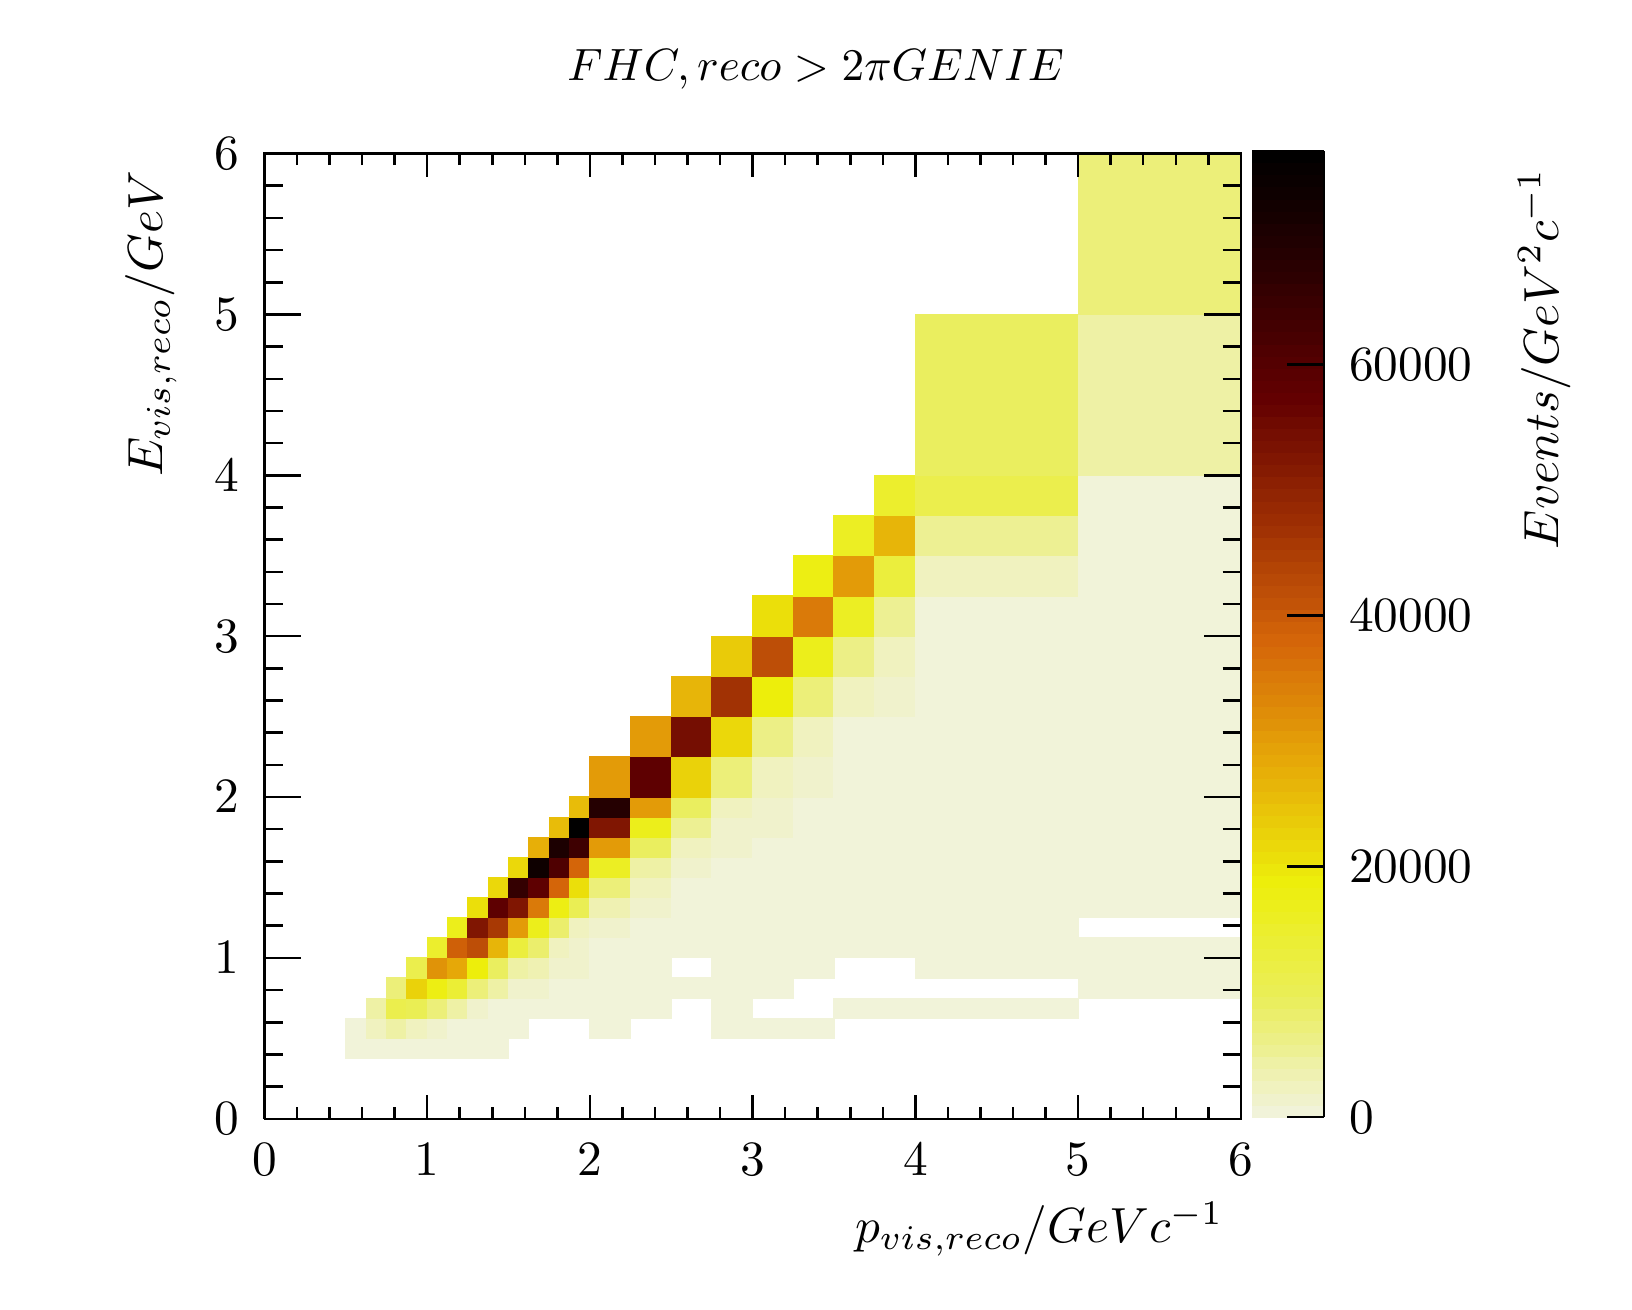
\begin{tikzpicture}
\pgfdeclareplotmark{cross} {
\pgfpathmoveto{\pgfpoint{-0.3\pgfplotmarksize}{\pgfplotmarksize}}
\pgfpathlineto{\pgfpoint{+0.3\pgfplotmarksize}{\pgfplotmarksize}}
\pgfpathlineto{\pgfpoint{+0.3\pgfplotmarksize}{0.3\pgfplotmarksize}}
\pgfpathlineto{\pgfpoint{+1\pgfplotmarksize}{0.3\pgfplotmarksize}}
\pgfpathlineto{\pgfpoint{+1\pgfplotmarksize}{-0.3\pgfplotmarksize}}
\pgfpathlineto{\pgfpoint{+0.3\pgfplotmarksize}{-0.3\pgfplotmarksize}}
\pgfpathlineto{\pgfpoint{+0.3\pgfplotmarksize}{-1.\pgfplotmarksize}}
\pgfpathlineto{\pgfpoint{-0.3\pgfplotmarksize}{-1.\pgfplotmarksize}}
\pgfpathlineto{\pgfpoint{-0.3\pgfplotmarksize}{-0.3\pgfplotmarksize}}
\pgfpathlineto{\pgfpoint{-1.\pgfplotmarksize}{-0.3\pgfplotmarksize}}
\pgfpathlineto{\pgfpoint{-1.\pgfplotmarksize}{0.3\pgfplotmarksize}}
\pgfpathlineto{\pgfpoint{-0.3\pgfplotmarksize}{0.3\pgfplotmarksize}}
\pgfpathclose
\pgfusepathqstroke
}
\pgfdeclareplotmark{cross*} {
\pgfpathmoveto{\pgfpoint{-0.3\pgfplotmarksize}{\pgfplotmarksize}}
\pgfpathlineto{\pgfpoint{+0.3\pgfplotmarksize}{\pgfplotmarksize}}
\pgfpathlineto{\pgfpoint{+0.3\pgfplotmarksize}{0.3\pgfplotmarksize}}
\pgfpathlineto{\pgfpoint{+1\pgfplotmarksize}{0.3\pgfplotmarksize}}
\pgfpathlineto{\pgfpoint{+1\pgfplotmarksize}{-0.3\pgfplotmarksize}}
\pgfpathlineto{\pgfpoint{+0.3\pgfplotmarksize}{-0.3\pgfplotmarksize}}
\pgfpathlineto{\pgfpoint{+0.3\pgfplotmarksize}{-1.\pgfplotmarksize}}
\pgfpathlineto{\pgfpoint{-0.3\pgfplotmarksize}{-1.\pgfplotmarksize}}
\pgfpathlineto{\pgfpoint{-0.3\pgfplotmarksize}{-0.3\pgfplotmarksize}}
\pgfpathlineto{\pgfpoint{-1.\pgfplotmarksize}{-0.3\pgfplotmarksize}}
\pgfpathlineto{\pgfpoint{-1.\pgfplotmarksize}{0.3\pgfplotmarksize}}
\pgfpathlineto{\pgfpoint{-0.3\pgfplotmarksize}{0.3\pgfplotmarksize}}
\pgfpathclose
\pgfusepathqfillstroke
}
\pgfdeclareplotmark{newstar} {
\pgfpathmoveto{\pgfqpoint{0pt}{\pgfplotmarksize}}
\pgfpathlineto{\pgfqpointpolar{44}{0.5\pgfplotmarksize}}
\pgfpathlineto{\pgfqpointpolar{18}{\pgfplotmarksize}}
\pgfpathlineto{\pgfqpointpolar{-20}{0.5\pgfplotmarksize}}
\pgfpathlineto{\pgfqpointpolar{-54}{\pgfplotmarksize}}
\pgfpathlineto{\pgfqpointpolar{-90}{0.5\pgfplotmarksize}}
\pgfpathlineto{\pgfqpointpolar{234}{\pgfplotmarksize}}
\pgfpathlineto{\pgfqpointpolar{198}{0.5\pgfplotmarksize}}
\pgfpathlineto{\pgfqpointpolar{162}{\pgfplotmarksize}}
\pgfpathlineto{\pgfqpointpolar{134}{0.5\pgfplotmarksize}}
\pgfpathclose
\pgfusepathqstroke
}
\pgfdeclareplotmark{newstar*} {
\pgfpathmoveto{\pgfqpoint{0pt}{\pgfplotmarksize}}
\pgfpathlineto{\pgfqpointpolar{44}{0.5\pgfplotmarksize}}
\pgfpathlineto{\pgfqpointpolar{18}{\pgfplotmarksize}}
\pgfpathlineto{\pgfqpointpolar{-20}{0.5\pgfplotmarksize}}
\pgfpathlineto{\pgfqpointpolar{-54}{\pgfplotmarksize}}
\pgfpathlineto{\pgfqpointpolar{-90}{0.5\pgfplotmarksize}}
\pgfpathlineto{\pgfqpointpolar{234}{\pgfplotmarksize}}
\pgfpathlineto{\pgfqpointpolar{198}{0.5\pgfplotmarksize}}
\pgfpathlineto{\pgfqpointpolar{162}{\pgfplotmarksize}}
\pgfpathlineto{\pgfqpointpolar{134}{0.5\pgfplotmarksize}}
\pgfpathclose
\pgfusepathqfillstroke
}
\definecolor{c}{rgb}{1,1,1};
\draw [color=c, fill=c] (0,0) rectangle (20,15.9197);
\draw [color=c, fill=c] (3,2.06957) rectangle (15.4,14.3278);
\definecolor{c}{rgb}{0,0,0};
\draw [c,line width=0.9] (3,2.06957) -- (3,14.3278) -- (15.4,14.3278) -- (15.4,2.06957) -- (3,2.06957);
\definecolor{c}{rgb}{1,1,1};
\draw [color=c, fill=c] (3,2.06957) rectangle (15.4,14.3278);
\definecolor{c}{rgb}{0,0,0};
\draw [c,line width=0.9] (3,2.06957) -- (3,14.3278) -- (15.4,14.3278) -- (15.4,2.06957) -- (3,2.06957);
\definecolor{c}{rgb}{0.945984,0.951044,0.850727};
\draw [color=c, fill=c] (4.03333,2.8357) rectangle (4.29167,3.09108);
\draw [color=c, fill=c] (4.29167,2.8357) rectangle (4.55,3.09108);
\draw [color=c, fill=c] (4.55,2.8357) rectangle (4.80833,3.09108);
\draw [color=c, fill=c] (4.80833,2.8357) rectangle (5.06667,3.09108);
\draw [color=c, fill=c] (5.06667,2.8357) rectangle (5.325,3.09108);
\draw [color=c, fill=c] (5.325,2.8357) rectangle (5.58333,3.09108);
\draw [color=c, fill=c] (5.58333,2.8357) rectangle (5.84167,3.09108);
\draw [color=c, fill=c] (5.84167,2.8357) rectangle (6.1,3.09108);
\draw [color=c, fill=c] (4.03333,3.09108) rectangle (4.29167,3.34646);
\definecolor{c}{rgb}{0.939911,0.947249,0.748261};
\draw [color=c, fill=c] (4.29167,3.09108) rectangle (4.55,3.34646);
\definecolor{c}{rgb}{0.933839,0.943453,0.645794};
\draw [color=c, fill=c] (4.55,3.09108) rectangle (4.80833,3.34646);
\definecolor{c}{rgb}{0.939911,0.947249,0.748261};
\draw [color=c, fill=c] (4.80833,3.09108) rectangle (5.06667,3.34646);
\definecolor{c}{rgb}{0.942948,0.949146,0.799494};
\draw [color=c, fill=c] (5.06667,3.09108) rectangle (5.325,3.34646);
\definecolor{c}{rgb}{0.945984,0.951044,0.850727};
\draw [color=c, fill=c] (5.325,3.09108) rectangle (5.58333,3.34646);
\draw [color=c, fill=c] (5.58333,3.09108) rectangle (5.84167,3.34646);
\draw [color=c, fill=c] (5.84167,3.09108) rectangle (6.1,3.34646);
\draw [color=c, fill=c] (6.1,3.09108) rectangle (6.35833,3.34646);
\draw [color=c, fill=c] (7.13333,3.09108) rectangle (7.65,3.34646);
\draw [color=c, fill=c] (8.68333,3.09108) rectangle (9.2,3.34646);
\draw [color=c, fill=c] (9.2,3.09108) rectangle (9.71667,3.34646);
\draw [color=c, fill=c] (9.71667,3.09108) rectangle (10.2333,3.34646);
\definecolor{c}{rgb}{0.933839,0.943453,0.645794};
\draw [color=c, fill=c] (4.29167,3.34646) rectangle (4.55,3.60184);
\definecolor{c}{rgb}{0.920221,0.933333,0.30049};
\draw [color=c, fill=c] (4.55,3.34646) rectangle (4.80833,3.60184);
\definecolor{c}{rgb}{0.919118,0.933333,0.331373};
\draw [color=c, fill=c] (4.80833,3.34646) rectangle (5.06667,3.60184);
\definecolor{c}{rgb}{0.923719,0.937128,0.475016};
\draw [color=c, fill=c] (5.06667,3.34646) rectangle (5.325,3.60184);
\definecolor{c}{rgb}{0.933839,0.943453,0.645794};
\draw [color=c, fill=c] (5.325,3.34646) rectangle (5.58333,3.60184);
\definecolor{c}{rgb}{0.942948,0.949146,0.799494};
\draw [color=c, fill=c] (5.58333,3.34646) rectangle (5.84167,3.60184);
\definecolor{c}{rgb}{0.945984,0.951044,0.850727};
\draw [color=c, fill=c] (5.84167,3.34646) rectangle (6.1,3.60184);
\draw [color=c, fill=c] (6.1,3.34646) rectangle (6.35833,3.60184);
\draw [color=c, fill=c] (6.35833,3.34646) rectangle (6.61667,3.60184);
\draw [color=c, fill=c] (6.61667,3.34646) rectangle (6.875,3.60184);
\draw [color=c, fill=c] (6.875,3.34646) rectangle (7.13333,3.60184);
\draw [color=c, fill=c] (7.13333,3.34646) rectangle (7.65,3.60184);
\draw [color=c, fill=c] (7.65,3.34646) rectangle (8.16667,3.60184);
\draw [color=c, fill=c] (8.68333,3.34646) rectangle (9.2,3.60184);
\draw [color=c, fill=c] (10.2333,3.34646) rectangle (10.75,3.60184);
\draw [color=c, fill=c] (10.75,3.34646) rectangle (11.2667,3.60184);
\draw [color=c, fill=c] (11.2667,3.34646) rectangle (13.3333,3.60184);
\definecolor{c}{rgb}{0.923719,0.937128,0.475016};
\draw [color=c, fill=c] (4.55,3.60184) rectangle (4.80833,3.85722);
\definecolor{c}{rgb}{0.91826,0.821814,0.0383578};
\draw [color=c, fill=c] (4.80833,3.60184) rectangle (5.06667,3.85722);
\definecolor{c}{rgb}{0.928309,0.933333,0.0740196};
\draw [color=c, fill=c] (5.06667,3.60184) rectangle (5.325,3.85722);
\definecolor{c}{rgb}{0.923529,0.933333,0.207843};
\draw [color=c, fill=c] (5.325,3.60184) rectangle (5.58333,3.85722);
\definecolor{c}{rgb}{0.923719,0.937128,0.475016};
\draw [color=c, fill=c] (5.58333,3.60184) rectangle (5.84167,3.85722);
\definecolor{c}{rgb}{0.933839,0.943453,0.645794};
\draw [color=c, fill=c] (5.84167,3.60184) rectangle (6.1,3.85722);
\definecolor{c}{rgb}{0.942948,0.949146,0.799494};
\draw [color=c, fill=c] (6.1,3.60184) rectangle (6.35833,3.85722);
\draw [color=c, fill=c] (6.35833,3.60184) rectangle (6.61667,3.85722);
\definecolor{c}{rgb}{0.945984,0.951044,0.850727};
\draw [color=c, fill=c] (6.61667,3.60184) rectangle (6.875,3.85722);
\draw [color=c, fill=c] (6.875,3.60184) rectangle (7.13333,3.85722);
\draw [color=c, fill=c] (7.13333,3.60184) rectangle (7.65,3.85722);
\draw [color=c, fill=c] (7.65,3.60184) rectangle (8.16667,3.85722);
\draw [color=c, fill=c] (8.16667,3.60184) rectangle (8.68333,3.85722);
\draw [color=c, fill=c] (8.68333,3.60184) rectangle (9.2,3.85722);
\draw [color=c, fill=c] (9.2,3.60184) rectangle (9.71667,3.85722);
\draw [color=c, fill=c] (13.3333,3.60184) rectangle (15.4,3.85722);
\definecolor{c}{rgb}{0.920221,0.933333,0.30049};
\draw [color=c, fill=c] (4.80833,3.85722) rectangle (5.06667,4.1126);
\definecolor{c}{rgb}{0.879902,0.576716,0.032598};
\draw [color=c, fill=c] (5.06667,3.85722) rectangle (5.325,4.1126);
\definecolor{c}{rgb}{0.901961,0.658824,0.0313726};
\draw [color=c, fill=c] (5.325,3.85722) rectangle (5.58333,4.1126);
\definecolor{c}{rgb}{0.929412,0.933333,0.0431373};
\draw [color=c, fill=c] (5.58333,3.85722) rectangle (5.84167,4.1126);
\definecolor{c}{rgb}{0.917647,0.933333,0.372549};
\draw [color=c, fill=c] (5.84167,3.85722) rectangle (6.1,4.1126);
\definecolor{c}{rgb}{0.933839,0.943453,0.645794};
\draw [color=c, fill=c] (6.1,3.85722) rectangle (6.35833,4.1126);
\definecolor{c}{rgb}{0.936875,0.945351,0.697027};
\draw [color=c, fill=c] (6.35833,3.85722) rectangle (6.61667,4.1126);
\definecolor{c}{rgb}{0.942948,0.949146,0.799494};
\draw [color=c, fill=c] (6.61667,3.85722) rectangle (6.875,4.1126);
\draw [color=c, fill=c] (6.875,3.85722) rectangle (7.13333,4.1126);
\definecolor{c}{rgb}{0.945984,0.951044,0.850727};
\draw [color=c, fill=c] (7.13333,3.85722) rectangle (7.65,4.1126);
\draw [color=c, fill=c] (7.65,3.85722) rectangle (8.16667,4.1126);
\draw [color=c, fill=c] (8.68333,3.85722) rectangle (9.2,4.1126);
\draw [color=c, fill=c] (9.2,3.85722) rectangle (9.71667,4.1126);
\draw [color=c, fill=c] (9.71667,3.85722) rectangle (10.2333,4.1126);
\draw [color=c, fill=c] (11.2667,3.85722) rectangle (13.3333,4.1126);
\draw [color=c, fill=c] (13.3333,3.85722) rectangle (15.4,4.1126);
\definecolor{c}{rgb}{0.924632,0.933333,0.176961};
\draw [color=c, fill=c] (5.06667,4.1126) rectangle (5.325,4.36798);
\definecolor{c}{rgb}{0.810784,0.37549,0.0330882};
\draw [color=c, fill=c] (5.325,4.1126) rectangle (5.58333,4.36798);
\definecolor{c}{rgb}{0.742157,0.306863,0.0257353};
\draw [color=c, fill=c] (5.58333,4.1126) rectangle (5.84167,4.36798);
\definecolor{c}{rgb}{0.907108,0.710294,0.0335784};
\draw [color=c, fill=c] (5.84167,4.1126) rectangle (6.1,4.36798);
\definecolor{c}{rgb}{0.922426,0.933333,0.238725};
\draw [color=c, fill=c] (6.1,4.1126) rectangle (6.35833,4.36798);
\definecolor{c}{rgb}{0.920683,0.935231,0.423782};
\draw [color=c, fill=c] (6.35833,4.1126) rectangle (6.61667,4.36798);
\definecolor{c}{rgb}{0.939911,0.947249,0.748261};
\draw [color=c, fill=c] (6.61667,4.1126) rectangle (6.875,4.36798);
\definecolor{c}{rgb}{0.942948,0.949146,0.799494};
\draw [color=c, fill=c] (6.875,4.1126) rectangle (7.13333,4.36798);
\definecolor{c}{rgb}{0.945984,0.951044,0.850727};
\draw [color=c, fill=c] (7.13333,4.1126) rectangle (7.65,4.36798);
\draw [color=c, fill=c] (7.65,4.1126) rectangle (8.16667,4.36798);
\draw [color=c, fill=c] (8.16667,4.1126) rectangle (8.68333,4.36798);
\draw [color=c, fill=c] (8.68333,4.1126) rectangle (9.2,4.36798);
\draw [color=c, fill=c] (9.2,4.1126) rectangle (9.71667,4.36798);
\draw [color=c, fill=c] (9.71667,4.1126) rectangle (10.2333,4.36798);
\draw [color=c, fill=c] (10.2333,4.1126) rectangle (10.75,4.36798);
\draw [color=c, fill=c] (10.75,4.1126) rectangle (11.2667,4.36798);
\draw [color=c, fill=c] (11.2667,4.1126) rectangle (13.3333,4.36798);
\draw [color=c, fill=c] (13.3333,4.1126) rectangle (15.4,4.36798);
\definecolor{c}{rgb}{0.927206,0.933333,0.104902};
\draw [color=c, fill=c] (5.325,4.36798) rectangle (5.58333,4.62336);
\definecolor{c}{rgb}{0.5,0.0882353,0.00784314};
\draw [color=c, fill=c] (5.58333,4.36798) rectangle (5.84167,4.62336);
\definecolor{c}{rgb}{0.659804,0.22451,0.0169118};
\draw [color=c, fill=c] (5.84167,4.36798) rectangle (6.1,4.62336);
\definecolor{c}{rgb}{0.888726,0.609559,0.0321078};
\draw [color=c, fill=c] (6.1,4.36798) rectangle (6.35833,4.62336);
\definecolor{c}{rgb}{0.927206,0.933333,0.104902};
\draw [color=c, fill=c] (6.35833,4.36798) rectangle (6.61667,4.62336);
\definecolor{c}{rgb}{0.920683,0.935231,0.423782};
\draw [color=c, fill=c] (6.61667,4.36798) rectangle (6.875,4.62336);
\definecolor{c}{rgb}{0.939911,0.947249,0.748261};
\draw [color=c, fill=c] (6.875,4.36798) rectangle (7.13333,4.62336);
\definecolor{c}{rgb}{0.942948,0.949146,0.799494};
\draw [color=c, fill=c] (7.13333,4.36798) rectangle (7.65,4.62336);
\definecolor{c}{rgb}{0.945984,0.951044,0.850727};
\draw [color=c, fill=c] (7.65,4.36798) rectangle (8.16667,4.62336);
\draw [color=c, fill=c] (8.16667,4.36798) rectangle (8.68333,4.62336);
\draw [color=c, fill=c] (8.68333,4.36798) rectangle (9.2,4.62336);
\draw [color=c, fill=c] (9.2,4.36798) rectangle (9.71667,4.62336);
\draw [color=c, fill=c] (9.71667,4.36798) rectangle (10.2333,4.62336);
\draw [color=c, fill=c] (10.2333,4.36798) rectangle (10.75,4.62336);
\draw [color=c, fill=c] (10.75,4.36798) rectangle (11.2667,4.62336);
\draw [color=c, fill=c] (11.2667,4.36798) rectangle (13.3333,4.62336);
\definecolor{c}{rgb}{0.923407,0.873284,0.0405637};
\draw [color=c, fill=c] (5.58333,4.62336) rectangle (5.84167,4.87873);
\definecolor{c}{rgb}{0.368382,0,0.00392157};
\draw [color=c, fill=c] (5.84167,4.62336) rectangle (6.1,4.87873);
\definecolor{c}{rgb}{0.5,0.0882353,0.00784314};
\draw [color=c, fill=c] (6.1,4.62336) rectangle (6.35833,4.87873);
\definecolor{c}{rgb}{0.853431,0.478186,0.0340686};
\draw [color=c, fill=c] (6.35833,4.62336) rectangle (6.61667,4.87873);
\definecolor{c}{rgb}{0.928309,0.933333,0.0740196};
\draw [color=c, fill=c] (6.61667,4.62336) rectangle (6.875,4.87873);
\definecolor{c}{rgb}{0.919118,0.933333,0.331373};
\draw [color=c, fill=c] (6.875,4.62336) rectangle (7.13333,4.87873);
\definecolor{c}{rgb}{0.936875,0.945351,0.697027};
\draw [color=c, fill=c] (7.13333,4.62336) rectangle (7.65,4.87873);
\definecolor{c}{rgb}{0.942948,0.949146,0.799494};
\draw [color=c, fill=c] (7.65,4.62336) rectangle (8.16667,4.87873);
\definecolor{c}{rgb}{0.945984,0.951044,0.850727};
\draw [color=c, fill=c] (8.16667,4.62336) rectangle (8.68333,4.87873);
\draw [color=c, fill=c] (8.68333,4.62336) rectangle (9.2,4.87873);
\draw [color=c, fill=c] (9.2,4.62336) rectangle (9.71667,4.87873);
\draw [color=c, fill=c] (9.71667,4.62336) rectangle (10.2333,4.87873);
\draw [color=c, fill=c] (10.2333,4.62336) rectangle (10.75,4.87873);
\draw [color=c, fill=c] (10.75,4.62336) rectangle (11.2667,4.87873);
\draw [color=c, fill=c] (11.2667,4.62336) rectangle (13.3333,4.87873);
\draw [color=c, fill=c] (13.3333,4.62336) rectangle (15.4,4.87873);
\definecolor{c}{rgb}{0.920833,0.847549,0.0394608};
\draw [color=c, fill=c] (5.84167,4.87873) rectangle (6.1,5.13411);
\definecolor{c}{rgb}{0.202941,0,0.00392157};
\draw [color=c, fill=c] (6.1,4.87873) rectangle (6.35833,5.13411);
\definecolor{c}{rgb}{0.368382,0,0.00392157};
\draw [color=c, fill=c] (6.35833,4.87873) rectangle (6.61667,5.13411);
\definecolor{c}{rgb}{0.831373,0.396078,0.0352941};
\draw [color=c, fill=c] (6.61667,4.87873) rectangle (6.875,5.13411);
\definecolor{c}{rgb}{0.923407,0.873284,0.0405637};
\draw [color=c, fill=c] (6.875,4.87873) rectangle (7.13333,5.13411);
\definecolor{c}{rgb}{0.923719,0.937128,0.475016};
\draw [color=c, fill=c] (7.13333,4.87873) rectangle (7.65,5.13411);
\definecolor{c}{rgb}{0.939911,0.947249,0.748261};
\draw [color=c, fill=c] (7.65,4.87873) rectangle (8.16667,5.13411);
\definecolor{c}{rgb}{0.945984,0.951044,0.850727};
\draw [color=c, fill=c] (8.16667,4.87873) rectangle (8.68333,5.13411);
\draw [color=c, fill=c] (8.68333,4.87873) rectangle (9.2,5.13411);
\draw [color=c, fill=c] (9.2,4.87873) rectangle (9.71667,5.13411);
\draw [color=c, fill=c] (9.71667,4.87873) rectangle (10.2333,5.13411);
\draw [color=c, fill=c] (10.2333,4.87873) rectangle (10.75,5.13411);
\draw [color=c, fill=c] (10.75,4.87873) rectangle (11.2667,5.13411);
\draw [color=c, fill=c] (11.2667,4.87873) rectangle (13.3333,5.13411);
\draw [color=c, fill=c] (13.3333,4.87873) rectangle (15.4,5.13411);
\definecolor{c}{rgb}{0.920833,0.847549,0.0394608};
\draw [color=c, fill=c] (6.1,5.13411) rectangle (6.35833,5.38949);
\definecolor{c}{rgb}{0.0551471,0,0.00122549};
\draw [color=c, fill=c] (6.35833,5.13411) rectangle (6.61667,5.38949);
\definecolor{c}{rgb}{0.308824,0,0.00392157};
\draw [color=c, fill=c] (6.61667,5.13411) rectangle (6.875,5.38949);
\definecolor{c}{rgb}{0.831373,0.396078,0.0352941};
\draw [color=c, fill=c] (6.875,5.13411) rectangle (7.13333,5.38949);
\definecolor{c}{rgb}{0.926103,0.933333,0.135784};
\draw [color=c, fill=c] (7.13333,5.13411) rectangle (7.65,5.38949);
\definecolor{c}{rgb}{0.933839,0.943453,0.645794};
\draw [color=c, fill=c] (7.65,5.13411) rectangle (8.16667,5.38949);
\definecolor{c}{rgb}{0.942948,0.949146,0.799494};
\draw [color=c, fill=c] (8.16667,5.13411) rectangle (8.68333,5.38949);
\definecolor{c}{rgb}{0.945984,0.951044,0.850727};
\draw [color=c, fill=c] (8.68333,5.13411) rectangle (9.2,5.38949);
\draw [color=c, fill=c] (9.2,5.13411) rectangle (9.71667,5.38949);
\draw [color=c, fill=c] (9.71667,5.13411) rectangle (10.2333,5.38949);
\draw [color=c, fill=c] (10.2333,5.13411) rectangle (10.75,5.38949);
\draw [color=c, fill=c] (10.75,5.13411) rectangle (11.2667,5.38949);
\draw [color=c, fill=c] (11.2667,5.13411) rectangle (13.3333,5.38949);
\draw [color=c, fill=c] (13.3333,5.13411) rectangle (15.4,5.38949);
\definecolor{c}{rgb}{0.904534,0.684559,0.0324755};
\draw [color=c, fill=c] (6.35833,5.38949) rectangle (6.61667,5.64487);
\definecolor{c}{rgb}{0.110294,0,0.00245098};
\draw [color=c, fill=c] (6.61667,5.38949) rectangle (6.875,5.64487);
\definecolor{c}{rgb}{0.242647,0,0.00392157};
\draw [color=c, fill=c] (6.875,5.38949) rectangle (7.13333,5.64487);
\definecolor{c}{rgb}{0.888726,0.609559,0.0321078};
\draw [color=c, fill=c] (7.13333,5.38949) rectangle (7.65,5.64487);
\definecolor{c}{rgb}{0.917647,0.933333,0.372549};
\draw [color=c, fill=c] (7.65,5.38949) rectangle (8.16667,5.64487);
\definecolor{c}{rgb}{0.939911,0.947249,0.748261};
\draw [color=c, fill=c] (8.16667,5.38949) rectangle (8.68333,5.64487);
\definecolor{c}{rgb}{0.942948,0.949146,0.799494};
\draw [color=c, fill=c] (8.68333,5.38949) rectangle (9.2,5.64487);
\definecolor{c}{rgb}{0.945984,0.951044,0.850727};
\draw [color=c, fill=c] (9.2,5.38949) rectangle (9.71667,5.64487);
\draw [color=c, fill=c] (9.71667,5.38949) rectangle (10.2333,5.64487);
\draw [color=c, fill=c] (10.2333,5.38949) rectangle (10.75,5.64487);
\draw [color=c, fill=c] (10.75,5.38949) rectangle (11.2667,5.64487);
\draw [color=c, fill=c] (11.2667,5.38949) rectangle (13.3333,5.64487);
\draw [color=c, fill=c] (13.3333,5.38949) rectangle (15.4,5.64487);
\definecolor{c}{rgb}{0.909681,0.736029,0.0346814};
\draw [color=c, fill=c] (6.61667,5.64487) rectangle (6.875,5.90025);
\definecolor{c}{rgb}{0.00551471,0,0.000122549};
\draw [color=c, fill=c] (6.875,5.64487) rectangle (7.13333,5.90025);
\definecolor{c}{rgb}{0.5,0.0882353,0.00784314};
\draw [color=c, fill=c] (7.13333,5.64487) rectangle (7.65,5.90025);
\definecolor{c}{rgb}{0.927206,0.933333,0.104902};
\draw [color=c, fill=c] (7.65,5.64487) rectangle (8.16667,5.90025);
\definecolor{c}{rgb}{0.929791,0.940923,0.577483};
\draw [color=c, fill=c] (8.16667,5.64487) rectangle (8.68333,5.90025);
\definecolor{c}{rgb}{0.942948,0.949146,0.799494};
\draw [color=c, fill=c] (8.68333,5.64487) rectangle (9.2,5.90025);
\draw [color=c, fill=c] (9.2,5.64487) rectangle (9.71667,5.90025);
\definecolor{c}{rgb}{0.945984,0.951044,0.850727};
\draw [color=c, fill=c] (9.71667,5.64487) rectangle (10.2333,5.90025);
\draw [color=c, fill=c] (10.2333,5.64487) rectangle (10.75,5.90025);
\draw [color=c, fill=c] (10.75,5.64487) rectangle (11.2667,5.90025);
\draw [color=c, fill=c] (11.2667,5.64487) rectangle (13.3333,5.90025);
\draw [color=c, fill=c] (13.3333,5.64487) rectangle (15.4,5.90025);
\definecolor{c}{rgb}{0.909681,0.736029,0.0346814};
\draw [color=c, fill=c] (6.875,5.90025) rectangle (7.13333,6.15563);
\definecolor{c}{rgb}{0.143382,0,0.00318627};
\draw [color=c, fill=c] (7.13333,5.90025) rectangle (7.65,6.15563);
\definecolor{c}{rgb}{0.888726,0.609559,0.0321078};
\draw [color=c, fill=c] (7.65,5.90025) rectangle (8.16667,6.15563);
\definecolor{c}{rgb}{0.917647,0.933333,0.372549};
\draw [color=c, fill=c] (8.16667,5.90025) rectangle (8.68333,6.15563);
\definecolor{c}{rgb}{0.939911,0.947249,0.748261};
\draw [color=c, fill=c] (8.68333,5.90025) rectangle (9.2,6.15563);
\definecolor{c}{rgb}{0.942948,0.949146,0.799494};
\draw [color=c, fill=c] (9.2,5.90025) rectangle (9.71667,6.15563);
\definecolor{c}{rgb}{0.945984,0.951044,0.850727};
\draw [color=c, fill=c] (9.71667,5.90025) rectangle (10.2333,6.15563);
\draw [color=c, fill=c] (10.2333,5.90025) rectangle (10.75,6.15563);
\draw [color=c, fill=c] (10.75,5.90025) rectangle (11.2667,6.15563);
\draw [color=c, fill=c] (11.2667,5.90025) rectangle (13.3333,6.15563);
\draw [color=c, fill=c] (13.3333,5.90025) rectangle (15.4,6.15563);
\definecolor{c}{rgb}{0.888726,0.609559,0.0321078};
\draw [color=c, fill=c] (7.13333,6.15563) rectangle (7.65,6.66639);
\definecolor{c}{rgb}{0.368382,0,0.00392157};
\draw [color=c, fill=c] (7.65,6.15563) rectangle (8.16667,6.66639);
\definecolor{c}{rgb}{0.91826,0.821814,0.0383578};
\draw [color=c, fill=c] (8.16667,6.15563) rectangle (8.68333,6.66639);
\definecolor{c}{rgb}{0.923719,0.937128,0.475016};
\draw [color=c, fill=c] (8.68333,6.15563) rectangle (9.2,6.66639);
\definecolor{c}{rgb}{0.939911,0.947249,0.748261};
\draw [color=c, fill=c] (9.2,6.15563) rectangle (9.71667,6.66639);
\definecolor{c}{rgb}{0.942948,0.949146,0.799494};
\draw [color=c, fill=c] (9.71667,6.15563) rectangle (10.2333,6.66639);
\definecolor{c}{rgb}{0.945984,0.951044,0.850727};
\draw [color=c, fill=c] (10.2333,6.15563) rectangle (10.75,6.66639);
\draw [color=c, fill=c] (10.75,6.15563) rectangle (11.2667,6.66639);
\draw [color=c, fill=c] (11.2667,6.15563) rectangle (13.3333,6.66639);
\draw [color=c, fill=c] (13.3333,6.15563) rectangle (15.4,6.66639);
\definecolor{c}{rgb}{0.888726,0.609559,0.0321078};
\draw [color=c, fill=c] (7.65,6.66639) rectangle (8.16667,7.17715);
\definecolor{c}{rgb}{0.458088,0.0551471,0.00637255};
\draw [color=c, fill=c] (8.16667,6.66639) rectangle (8.68333,7.17715);
\definecolor{c}{rgb}{0.920833,0.847549,0.0394608};
\draw [color=c, fill=c] (8.68333,6.66639) rectangle (9.2,7.17715);
\definecolor{c}{rgb}{0.926755,0.939026,0.526249};
\draw [color=c, fill=c] (9.2,6.66639) rectangle (9.71667,7.17715);
\definecolor{c}{rgb}{0.939911,0.947249,0.748261};
\draw [color=c, fill=c] (9.71667,6.66639) rectangle (10.2333,7.17715);
\definecolor{c}{rgb}{0.945984,0.951044,0.850727};
\draw [color=c, fill=c] (10.2333,6.66639) rectangle (10.75,7.17715);
\draw [color=c, fill=c] (10.75,6.66639) rectangle (11.2667,7.17715);
\draw [color=c, fill=c] (11.2667,6.66639) rectangle (13.3333,7.17715);
\draw [color=c, fill=c] (13.3333,6.66639) rectangle (15.4,7.17715);
\definecolor{c}{rgb}{0.907108,0.710294,0.0335784};
\draw [color=c, fill=c] (8.16667,7.17715) rectangle (8.68333,7.6879);
\definecolor{c}{rgb}{0.632353,0.197059,0.0139706};
\draw [color=c, fill=c] (8.68333,7.17715) rectangle (9.2,7.6879);
\definecolor{c}{rgb}{0.929412,0.933333,0.0431373};
\draw [color=c, fill=c] (9.2,7.17715) rectangle (9.71667,7.6879);
\definecolor{c}{rgb}{0.923719,0.937128,0.475016};
\draw [color=c, fill=c] (9.71667,7.17715) rectangle (10.2333,7.6879);
\definecolor{c}{rgb}{0.939911,0.947249,0.748261};
\draw [color=c, fill=c] (10.2333,7.17715) rectangle (10.75,7.6879);
\definecolor{c}{rgb}{0.942948,0.949146,0.799494};
\draw [color=c, fill=c] (10.75,7.17715) rectangle (11.2667,7.6879);
\definecolor{c}{rgb}{0.945984,0.951044,0.850727};
\draw [color=c, fill=c] (11.2667,7.17715) rectangle (13.3333,7.6879);
\draw [color=c, fill=c] (13.3333,7.17715) rectangle (15.4,7.6879);
\definecolor{c}{rgb}{0.915686,0.796078,0.0372549};
\draw [color=c, fill=c] (8.68333,7.6879) rectangle (9.2,8.19866);
\definecolor{c}{rgb}{0.742157,0.306863,0.0257353};
\draw [color=c, fill=c] (9.2,7.6879) rectangle (9.71667,8.19866);
\definecolor{c}{rgb}{0.927206,0.933333,0.104902};
\draw [color=c, fill=c] (9.71667,7.6879) rectangle (10.2333,8.19866);
\definecolor{c}{rgb}{0.926755,0.939026,0.526249};
\draw [color=c, fill=c] (10.2333,7.6879) rectangle (10.75,8.19866);
\definecolor{c}{rgb}{0.939911,0.947249,0.748261};
\draw [color=c, fill=c] (10.75,7.6879) rectangle (11.2667,8.19866);
\definecolor{c}{rgb}{0.945984,0.951044,0.850727};
\draw [color=c, fill=c] (11.2667,7.6879) rectangle (13.3333,8.19866);
\draw [color=c, fill=c] (13.3333,7.6879) rectangle (15.4,8.19866);
\definecolor{c}{rgb}{0.923407,0.873284,0.0405637};
\draw [color=c, fill=c] (9.2,8.19866) rectangle (9.71667,8.70942);
\definecolor{c}{rgb}{0.853431,0.478186,0.0340686};
\draw [color=c, fill=c] (9.71667,8.19866) rectangle (10.2333,8.70942);
\definecolor{c}{rgb}{0.926103,0.933333,0.135784};
\draw [color=c, fill=c] (10.2333,8.19866) rectangle (10.75,8.70942);
\definecolor{c}{rgb}{0.929791,0.940923,0.577483};
\draw [color=c, fill=c] (10.75,8.19866) rectangle (11.2667,8.70942);
\definecolor{c}{rgb}{0.945984,0.951044,0.850727};
\draw [color=c, fill=c] (11.2667,8.19866) rectangle (13.3333,8.70942);
\draw [color=c, fill=c] (13.3333,8.19866) rectangle (15.4,8.70942);
\definecolor{c}{rgb}{0.928309,0.933333,0.0740196};
\draw [color=c, fill=c] (9.71667,8.70942) rectangle (10.2333,9.22018);
\definecolor{c}{rgb}{0.888726,0.609559,0.0321078};
\draw [color=c, fill=c] (10.2333,8.70942) rectangle (10.75,9.22018);
\definecolor{c}{rgb}{0.922426,0.933333,0.238725};
\draw [color=c, fill=c] (10.75,8.70942) rectangle (11.2667,9.22018);
\definecolor{c}{rgb}{0.939911,0.947249,0.748261};
\draw [color=c, fill=c] (11.2667,8.70942) rectangle (13.3333,9.22018);
\definecolor{c}{rgb}{0.945984,0.951044,0.850727};
\draw [color=c, fill=c] (13.3333,8.70942) rectangle (15.4,9.22018);
\definecolor{c}{rgb}{0.926103,0.933333,0.135784};
\draw [color=c, fill=c] (10.2333,9.22018) rectangle (10.75,9.73094);
\definecolor{c}{rgb}{0.907108,0.710294,0.0335784};
\draw [color=c, fill=c] (10.75,9.22018) rectangle (11.2667,9.73094);
\definecolor{c}{rgb}{0.929791,0.940923,0.577483};
\draw [color=c, fill=c] (11.2667,9.22018) rectangle (13.3333,9.73094);
\definecolor{c}{rgb}{0.945984,0.951044,0.850727};
\draw [color=c, fill=c] (13.3333,9.22018) rectangle (15.4,9.73094);
\definecolor{c}{rgb}{0.924632,0.933333,0.176961};
\draw [color=c, fill=c] (10.75,9.73094) rectangle (11.2667,10.2417);
\definecolor{c}{rgb}{0.920221,0.933333,0.30049};
\draw [color=c, fill=c] (11.2667,9.73094) rectangle (13.3333,10.2417);
\definecolor{c}{rgb}{0.945984,0.951044,0.850727};
\draw [color=c, fill=c] (13.3333,9.73094) rectangle (15.4,10.2417);
\definecolor{c}{rgb}{0.917647,0.933333,0.372549};
\draw [color=c, fill=c] (11.2667,10.2417) rectangle (13.3333,12.2847);
\definecolor{c}{rgb}{0.933839,0.943453,0.645794};
\draw [color=c, fill=c] (13.3333,10.2417) rectangle (15.4,12.2847);
\definecolor{c}{rgb}{0.923719,0.937128,0.475016};
\draw [color=c, fill=c] (13.3333,12.2847) rectangle (15.4,14.3278);
\definecolor{c}{rgb}{0,0,0};
\draw [c,line width=0.9] (3,2.06957) -- (15.4,2.06957);
\draw [c,line width=0.9] (3,2.36567) -- (3,2.06957);
\draw [c,line width=0.9] (3.41333,2.21762) -- (3.41333,2.06957);
\draw [c,line width=0.9] (3.82667,2.21762) -- (3.82667,2.06957);
\draw [c,line width=0.9] (4.24,2.21762) -- (4.24,2.06957);
\draw [c,line width=0.9] (4.65333,2.21762) -- (4.65333,2.06957);
\draw [c,line width=0.9] (5.06667,2.36567) -- (5.06667,2.06957);
\draw [c,line width=0.9] (5.48,2.21762) -- (5.48,2.06957);
\draw [c,line width=0.9] (5.89333,2.21762) -- (5.89333,2.06957);
\draw [c,line width=0.9] (6.30667,2.21762) -- (6.30667,2.06957);
\draw [c,line width=0.9] (6.72,2.21762) -- (6.72,2.06957);
\draw [c,line width=0.9] (7.13333,2.36567) -- (7.13333,2.06957);
\draw [c,line width=0.9] (7.54667,2.21762) -- (7.54667,2.06957);
\draw [c,line width=0.9] (7.96,2.21762) -- (7.96,2.06957);
\draw [c,line width=0.9] (8.37333,2.21762) -- (8.37333,2.06957);
\draw [c,line width=0.9] (8.78667,2.21762) -- (8.78667,2.06957);
\draw [c,line width=0.9] (9.2,2.36567) -- (9.2,2.06957);
\draw [c,line width=0.9] (9.61333,2.21762) -- (9.61333,2.06957);
\draw [c,line width=0.9] (10.0267,2.21762) -- (10.0267,2.06957);
\draw [c,line width=0.9] (10.44,2.21762) -- (10.44,2.06957);
\draw [c,line width=0.9] (10.8533,2.21762) -- (10.8533,2.06957);
\draw [c,line width=0.9] (11.2667,2.36567) -- (11.2667,2.06957);
\draw [c,line width=0.9] (11.68,2.21762) -- (11.68,2.06957);
\draw [c,line width=0.9] (12.0933,2.21762) -- (12.0933,2.06957);
\draw [c,line width=0.9] (12.5067,2.21762) -- (12.5067,2.06957);
\draw [c,line width=0.9] (12.92,2.21762) -- (12.92,2.06957);
\draw [c,line width=0.9] (13.3333,2.36567) -- (13.3333,2.06957);
\draw [c,line width=0.9] (13.7467,2.21762) -- (13.7467,2.06957);
\draw [c,line width=0.9] (14.16,2.21762) -- (14.16,2.06957);
\draw [c,line width=0.9] (14.5733,2.21762) -- (14.5733,2.06957);
\draw [c,line width=0.9] (14.9867,2.21762) -- (14.9867,2.06957);
\draw [c,line width=0.9] (15.4,2.36567) -- (15.4,2.06957);
\draw [anchor=base] (3,1.35318) node[scale=1.78272, color=c, rotate=0]{0};
\draw [anchor=base] (5.06667,1.35318) node[scale=1.78272, color=c, rotate=0]{1};
\draw [anchor=base] (7.13333,1.35318) node[scale=1.78272, color=c, rotate=0]{2};
\draw [anchor=base] (9.2,1.35318) node[scale=1.78272, color=c, rotate=0]{3};
\draw [anchor=base] (11.2667,1.35318) node[scale=1.78272, color=c, rotate=0]{4};
\draw [anchor=base] (13.3333,1.35318) node[scale=1.78272, color=c, rotate=0]{5};
\draw [anchor=base] (15.4,1.35318) node[scale=1.78272, color=c, rotate=0]{6};
\draw [anchor= east] (15.4,0.668629) node[scale=1.78272, color=c, rotate=0]{$ p_{vis, reco} / GeV c^{-1}$};
\draw [c,line width=0.9] (3,14.3278) -- (15.4,14.3278);
\draw [c,line width=0.9] (3,14.0317) -- (3,14.3278);
\draw [c,line width=0.9] (3.41333,14.1797) -- (3.41333,14.3278);
\draw [c,line width=0.9] (3.82667,14.1797) -- (3.82667,14.3278);
\draw [c,line width=0.9] (4.24,14.1797) -- (4.24,14.3278);
\draw [c,line width=0.9] (4.65333,14.1797) -- (4.65333,14.3278);
\draw [c,line width=0.9] (5.06667,14.0317) -- (5.06667,14.3278);
\draw [c,line width=0.9] (5.48,14.1797) -- (5.48,14.3278);
\draw [c,line width=0.9] (5.89333,14.1797) -- (5.89333,14.3278);
\draw [c,line width=0.9] (6.30667,14.1797) -- (6.30667,14.3278);
\draw [c,line width=0.9] (6.72,14.1797) -- (6.72,14.3278);
\draw [c,line width=0.9] (7.13333,14.0317) -- (7.13333,14.3278);
\draw [c,line width=0.9] (7.54667,14.1797) -- (7.54667,14.3278);
\draw [c,line width=0.9] (7.96,14.1797) -- (7.96,14.3278);
\draw [c,line width=0.9] (8.37333,14.1797) -- (8.37333,14.3278);
\draw [c,line width=0.9] (8.78667,14.1797) -- (8.78667,14.3278);
\draw [c,line width=0.9] (9.2,14.0317) -- (9.2,14.3278);
\draw [c,line width=0.9] (9.61333,14.1797) -- (9.61333,14.3278);
\draw [c,line width=0.9] (10.0267,14.1797) -- (10.0267,14.3278);
\draw [c,line width=0.9] (10.44,14.1797) -- (10.44,14.3278);
\draw [c,line width=0.9] (10.8533,14.1797) -- (10.8533,14.3278);
\draw [c,line width=0.9] (11.2667,14.0317) -- (11.2667,14.3278);
\draw [c,line width=0.9] (11.68,14.1797) -- (11.68,14.3278);
\draw [c,line width=0.9] (12.0933,14.1797) -- (12.0933,14.3278);
\draw [c,line width=0.9] (12.5067,14.1797) -- (12.5067,14.3278);
\draw [c,line width=0.9] (12.92,14.1797) -- (12.92,14.3278);
\draw [c,line width=0.9] (13.3333,14.0317) -- (13.3333,14.3278);
\draw [c,line width=0.9] (13.7467,14.1797) -- (13.7467,14.3278);
\draw [c,line width=0.9] (14.16,14.1797) -- (14.16,14.3278);
\draw [c,line width=0.9] (14.5733,14.1797) -- (14.5733,14.3278);
\draw [c,line width=0.9] (14.9867,14.1797) -- (14.9867,14.3278);
\draw [c,line width=0.9] (15.4,14.0317) -- (15.4,14.3278);
\draw [c,line width=0.9] (3,2.06957) -- (3,14.3278);
\draw [c,line width=0.9] (3.462,2.06957) -- (3,2.06957);
\draw [c,line width=0.9] (3.231,2.47817) -- (3,2.47817);
\draw [c,line width=0.9] (3.231,2.88678) -- (3,2.88678);
\draw [c,line width=0.9] (3.231,3.29538) -- (3,3.29538);
\draw [c,line width=0.9] (3.231,3.70399) -- (3,3.70399);
\draw [c,line width=0.9] (3.462,4.1126) -- (3,4.1126);
\draw [c,line width=0.9] (3.231,4.5212) -- (3,4.5212);
\draw [c,line width=0.9] (3.231,4.92981) -- (3,4.92981);
\draw [c,line width=0.9] (3.231,5.33842) -- (3,5.33842);
\draw [c,line width=0.9] (3.231,5.74702) -- (3,5.74702);
\draw [c,line width=0.9] (3.462,6.15563) -- (3,6.15563);
\draw [c,line width=0.9] (3.231,6.56424) -- (3,6.56424);
\draw [c,line width=0.9] (3.231,6.97284) -- (3,6.97284);
\draw [c,line width=0.9] (3.231,7.38145) -- (3,7.38145);
\draw [c,line width=0.9] (3.231,7.79006) -- (3,7.79006);
\draw [c,line width=0.9] (3.462,8.19866) -- (3,8.19866);
\draw [c,line width=0.9] (3.231,8.60727) -- (3,8.60727);
\draw [c,line width=0.9] (3.231,9.01587) -- (3,9.01587);
\draw [c,line width=0.9] (3.231,9.42448) -- (3,9.42448);
\draw [c,line width=0.9] (3.231,9.83309) -- (3,9.83309);
\draw [c,line width=0.9] (3.462,10.2417) -- (3,10.2417);
\draw [c,line width=0.9] (3.231,10.6503) -- (3,10.6503);
\draw [c,line width=0.9] (3.231,11.0589) -- (3,11.0589);
\draw [c,line width=0.9] (3.231,11.4675) -- (3,11.4675);
\draw [c,line width=0.9] (3.231,11.8761) -- (3,11.8761);
\draw [c,line width=0.9] (3.462,12.2847) -- (3,12.2847);
\draw [c,line width=0.9] (3.231,12.6933) -- (3,12.6933);
\draw [c,line width=0.9] (3.231,13.1019) -- (3,13.1019);
\draw [c,line width=0.9] (3.231,13.5105) -- (3,13.5105);
\draw [c,line width=0.9] (3.231,13.9192) -- (3,13.9192);
\draw [c,line width=0.9] (3.462,14.3278) -- (3,14.3278);
\draw [anchor= east] (2.9,2.06957) node[scale=1.78272, color=c, rotate=0]{0};
\draw [anchor= east] (2.9,4.1126) node[scale=1.78272, color=c, rotate=0]{1};
\draw [anchor= east] (2.9,6.15563) node[scale=1.78272, color=c, rotate=0]{2};
\draw [anchor= east] (2.9,8.19866) node[scale=1.78272, color=c, rotate=0]{3};
\draw [anchor= east] (2.9,10.2417) node[scale=1.78272, color=c, rotate=0]{4};
\draw [anchor= east] (2.9,12.2847) node[scale=1.78272, color=c, rotate=0]{5};
\draw [anchor= east] (2.9,14.3278) node[scale=1.78272, color=c, rotate=0]{6};
\draw [anchor= east] (1.56,14.3278) node[scale=1.78272, color=c, rotate=90]{$ E_{vis, reco} / GeV$};
\draw [c,line width=0.9] (15.4,2.06957) -- (15.4,14.3278);
\draw [c,line width=0.9] (14.938,2.06957) -- (15.4,2.06957);
\draw [c,line width=0.9] (15.169,2.47817) -- (15.4,2.47817);
\draw [c,line width=0.9] (15.169,2.88678) -- (15.4,2.88678);
\draw [c,line width=0.9] (15.169,3.29538) -- (15.4,3.29538);
\draw [c,line width=0.9] (15.169,3.70399) -- (15.4,3.70399);
\draw [c,line width=0.9] (14.938,4.1126) -- (15.4,4.1126);
\draw [c,line width=0.9] (15.169,4.5212) -- (15.4,4.5212);
\draw [c,line width=0.9] (15.169,4.92981) -- (15.4,4.92981);
\draw [c,line width=0.9] (15.169,5.33842) -- (15.4,5.33842);
\draw [c,line width=0.9] (15.169,5.74702) -- (15.4,5.74702);
\draw [c,line width=0.9] (14.938,6.15563) -- (15.4,6.15563);
\draw [c,line width=0.9] (15.169,6.56424) -- (15.4,6.56424);
\draw [c,line width=0.9] (15.169,6.97284) -- (15.4,6.97284);
\draw [c,line width=0.9] (15.169,7.38145) -- (15.4,7.38145);
\draw [c,line width=0.9] (15.169,7.79006) -- (15.4,7.79006);
\draw [c,line width=0.9] (14.938,8.19866) -- (15.4,8.19866);
\draw [c,line width=0.9] (15.169,8.60727) -- (15.4,8.60727);
\draw [c,line width=0.9] (15.169,9.01587) -- (15.4,9.01587);
\draw [c,line width=0.9] (15.169,9.42448) -- (15.4,9.42448);
\draw [c,line width=0.9] (15.169,9.83309) -- (15.4,9.83309);
\draw [c,line width=0.9] (14.938,10.2417) -- (15.4,10.2417);
\draw [c,line width=0.9] (15.169,10.6503) -- (15.4,10.6503);
\draw [c,line width=0.9] (15.169,11.0589) -- (15.4,11.0589);
\draw [c,line width=0.9] (15.169,11.4675) -- (15.4,11.4675);
\draw [c,line width=0.9] (15.169,11.8761) -- (15.4,11.8761);
\draw [c,line width=0.9] (14.938,12.2847) -- (15.4,12.2847);
\draw [c,line width=0.9] (15.169,12.6933) -- (15.4,12.6933);
\draw [c,line width=0.9] (15.169,13.1019) -- (15.4,13.1019);
\draw [c,line width=0.9] (15.169,13.5105) -- (15.4,13.5105);
\draw [c,line width=0.9] (15.169,13.9192) -- (15.4,13.9192);
\draw [c,line width=0.9] (14.938,14.3278) -- (15.4,14.3278);
\definecolor{c}{rgb}{0.945984,0.951044,0.850727};
\draw [color=c, fill=c] (15.5518,2.0903) rectangle (16.4548,2.24373);
\definecolor{c}{rgb}{0.942948,0.949146,0.799494};
\draw [color=c, fill=c] (15.5518,2.24373) rectangle (16.4548,2.39716);
\definecolor{c}{rgb}{0.939911,0.947249,0.748261};
\draw [color=c, fill=c] (15.5518,2.39716) rectangle (16.4548,2.55059);
\definecolor{c}{rgb}{0.936875,0.945351,0.697027};
\draw [color=c, fill=c] (15.5518,2.55059) rectangle (16.4548,2.70401);
\definecolor{c}{rgb}{0.933839,0.943453,0.645794};
\draw [color=c, fill=c] (15.5518,2.70401) rectangle (16.4548,2.85744);
\definecolor{c}{rgb}{0.929791,0.940923,0.577483};
\draw [color=c, fill=c] (15.5518,2.85744) rectangle (16.4548,3.01087);
\definecolor{c}{rgb}{0.926755,0.939026,0.526249};
\draw [color=c, fill=c] (15.5518,3.01087) rectangle (16.4548,3.1643);
\definecolor{c}{rgb}{0.923719,0.937128,0.475016};
\draw [color=c, fill=c] (15.5518,3.1643) rectangle (16.4548,3.31773);
\definecolor{c}{rgb}{0.920683,0.935231,0.423782};
\draw [color=c, fill=c] (15.5518,3.31773) rectangle (16.4548,3.47115);
\definecolor{c}{rgb}{0.917647,0.933333,0.372549};
\draw [color=c, fill=c] (15.5518,3.47115) rectangle (16.4548,3.62458);
\definecolor{c}{rgb}{0.919118,0.933333,0.331373};
\draw [color=c, fill=c] (15.5518,3.62458) rectangle (16.4548,3.77801);
\definecolor{c}{rgb}{0.920221,0.933333,0.30049};
\draw [color=c, fill=c] (15.5518,3.77801) rectangle (16.4548,3.93144);
\definecolor{c}{rgb}{0.921324,0.933333,0.269608};
\draw [color=c, fill=c] (15.5518,3.93144) rectangle (16.4548,4.08487);
\definecolor{c}{rgb}{0.922426,0.933333,0.238725};
\draw [color=c, fill=c] (15.5518,4.08487) rectangle (16.4548,4.23829);
\definecolor{c}{rgb}{0.923529,0.933333,0.207843};
\draw [color=c, fill=c] (15.5518,4.23829) rectangle (16.4548,4.39172);
\definecolor{c}{rgb}{0.924632,0.933333,0.176961};
\draw [color=c, fill=c] (15.5518,4.39172) rectangle (16.4548,4.54515);
\definecolor{c}{rgb}{0.926103,0.933333,0.135784};
\draw [color=c, fill=c] (15.5518,4.54515) rectangle (16.4548,4.69858);
\definecolor{c}{rgb}{0.927206,0.933333,0.104902};
\draw [color=c, fill=c] (15.5518,4.69858) rectangle (16.4548,4.85201);
\definecolor{c}{rgb}{0.928309,0.933333,0.0740196};
\draw [color=c, fill=c] (15.5518,4.85201) rectangle (16.4548,5.00543);
\definecolor{c}{rgb}{0.929412,0.933333,0.0431373};
\draw [color=c, fill=c] (15.5518,5.00543) rectangle (16.4548,5.15886);
\definecolor{c}{rgb}{0.926838,0.907598,0.0420343};
\draw [color=c, fill=c] (15.5518,5.15886) rectangle (16.4548,5.31229);
\definecolor{c}{rgb}{0.923407,0.873284,0.0405637};
\draw [color=c, fill=c] (15.5518,5.31229) rectangle (16.4548,5.46572);
\definecolor{c}{rgb}{0.920833,0.847549,0.0394608};
\draw [color=c, fill=c] (15.5518,5.46572) rectangle (16.4548,5.61915);
\definecolor{c}{rgb}{0.91826,0.821814,0.0383578};
\draw [color=c, fill=c] (15.5518,5.61915) rectangle (16.4548,5.77257);
\definecolor{c}{rgb}{0.915686,0.796078,0.0372549};
\draw [color=c, fill=c] (15.5518,5.77257) rectangle (16.4548,5.926);
\definecolor{c}{rgb}{0.913113,0.770343,0.036152};
\draw [color=c, fill=c] (15.5518,5.926) rectangle (16.4548,6.07943);
\definecolor{c}{rgb}{0.909681,0.736029,0.0346814};
\draw [color=c, fill=c] (15.5518,6.07943) rectangle (16.4548,6.23286);
\definecolor{c}{rgb}{0.907108,0.710294,0.0335784};
\draw [color=c, fill=c] (15.5518,6.23286) rectangle (16.4548,6.38629);
\definecolor{c}{rgb}{0.904534,0.684559,0.0324755};
\draw [color=c, fill=c] (15.5518,6.38629) rectangle (16.4548,6.53972);
\definecolor{c}{rgb}{0.901961,0.658824,0.0313726};
\draw [color=c, fill=c] (15.5518,6.53972) rectangle (16.4548,6.69314);
\definecolor{c}{rgb}{0.895343,0.634191,0.0317402};
\draw [color=c, fill=c] (15.5518,6.69314) rectangle (16.4548,6.84657);
\definecolor{c}{rgb}{0.888726,0.609559,0.0321078};
\draw [color=c, fill=c] (15.5518,6.84657) rectangle (16.4548,7);
\definecolor{c}{rgb}{0.879902,0.576716,0.032598};
\draw [color=c, fill=c] (15.5518,7) rectangle (16.4548,7.15343);
\definecolor{c}{rgb}{0.873284,0.552083,0.0329657};
\draw [color=c, fill=c] (15.5518,7.15343) rectangle (16.4548,7.30686);
\definecolor{c}{rgb}{0.866667,0.527451,0.0333333};
\draw [color=c, fill=c] (15.5518,7.30686) rectangle (16.4548,7.46028);
\definecolor{c}{rgb}{0.860049,0.502819,0.033701};
\draw [color=c, fill=c] (15.5518,7.46028) rectangle (16.4548,7.61371);
\definecolor{c}{rgb}{0.853431,0.478186,0.0340686};
\draw [color=c, fill=c] (15.5518,7.61371) rectangle (16.4548,7.76714);
\definecolor{c}{rgb}{0.844608,0.445343,0.0345588};
\draw [color=c, fill=c] (15.5518,7.76714) rectangle (16.4548,7.92057);
\definecolor{c}{rgb}{0.83799,0.420711,0.0349265};
\draw [color=c, fill=c] (15.5518,7.92057) rectangle (16.4548,8.074);
\definecolor{c}{rgb}{0.831373,0.396078,0.0352941};
\draw [color=c, fill=c] (15.5518,8.074) rectangle (16.4548,8.22742);
\definecolor{c}{rgb}{0.810784,0.37549,0.0330882};
\draw [color=c, fill=c] (15.5518,8.22742) rectangle (16.4548,8.38085);
\definecolor{c}{rgb}{0.790196,0.354902,0.0308824};
\draw [color=c, fill=c] (15.5518,8.38085) rectangle (16.4548,8.53428);
\definecolor{c}{rgb}{0.762745,0.327451,0.0279412};
\draw [color=c, fill=c] (15.5518,8.53428) rectangle (16.4548,8.68771);
\definecolor{c}{rgb}{0.742157,0.306863,0.0257353};
\draw [color=c, fill=c] (15.5518,8.68771) rectangle (16.4548,8.84114);
\definecolor{c}{rgb}{0.721569,0.286275,0.0235294};
\draw [color=c, fill=c] (15.5518,8.84114) rectangle (16.4548,8.99457);
\definecolor{c}{rgb}{0.70098,0.265686,0.0213235};
\draw [color=c, fill=c] (15.5518,8.99457) rectangle (16.4548,9.14799);
\definecolor{c}{rgb}{0.680392,0.245098,0.0191176};
\draw [color=c, fill=c] (15.5518,9.14799) rectangle (16.4548,9.30142);
\definecolor{c}{rgb}{0.659804,0.22451,0.0169118};
\draw [color=c, fill=c] (15.5518,9.30142) rectangle (16.4548,9.45485);
\definecolor{c}{rgb}{0.632353,0.197059,0.0139706};
\draw [color=c, fill=c] (15.5518,9.45485) rectangle (16.4548,9.60828);
\definecolor{c}{rgb}{0.611765,0.176471,0.0117647};
\draw [color=c, fill=c] (15.5518,9.60828) rectangle (16.4548,9.76171);
\definecolor{c}{rgb}{0.590809,0.159926,0.0110294};
\draw [color=c, fill=c] (15.5518,9.76171) rectangle (16.4548,9.91513);
\definecolor{c}{rgb}{0.569853,0.143382,0.0102941};
\draw [color=c, fill=c] (15.5518,9.91513) rectangle (16.4548,10.0686);
\definecolor{c}{rgb}{0.548897,0.126838,0.00955882};
\draw [color=c, fill=c] (15.5518,10.0686) rectangle (16.4548,10.222);
\definecolor{c}{rgb}{0.520956,0.104779,0.00857843};
\draw [color=c, fill=c] (15.5518,10.222) rectangle (16.4548,10.3754);
\definecolor{c}{rgb}{0.5,0.0882353,0.00784314};
\draw [color=c, fill=c] (15.5518,10.3754) rectangle (16.4548,10.5288);
\definecolor{c}{rgb}{0.479044,0.0716912,0.00710784};
\draw [color=c, fill=c] (15.5518,10.5288) rectangle (16.4548,10.6823);
\definecolor{c}{rgb}{0.458088,0.0551471,0.00637255};
\draw [color=c, fill=c] (15.5518,10.6823) rectangle (16.4548,10.8357);
\definecolor{c}{rgb}{0.437132,0.0386029,0.00563726};
\draw [color=c, fill=c] (15.5518,10.8357) rectangle (16.4548,10.9891);
\definecolor{c}{rgb}{0.409191,0.0165441,0.00465686};
\draw [color=c, fill=c] (15.5518,10.9891) rectangle (16.4548,11.1426);
\definecolor{c}{rgb}{0.388235,0,0.00392157};
\draw [color=c, fill=c] (15.5518,11.1426) rectangle (16.4548,11.296);
\definecolor{c}{rgb}{0.368382,0,0.00392157};
\draw [color=c, fill=c] (15.5518,11.296) rectangle (16.4548,11.4494);
\definecolor{c}{rgb}{0.348529,0,0.00392157};
\draw [color=c, fill=c] (15.5518,11.4494) rectangle (16.4548,11.6028);
\definecolor{c}{rgb}{0.328676,0,0.00392157};
\draw [color=c, fill=c] (15.5518,11.6028) rectangle (16.4548,11.7563);
\definecolor{c}{rgb}{0.308824,0,0.00392157};
\draw [color=c, fill=c] (15.5518,11.7563) rectangle (16.4548,11.9097);
\definecolor{c}{rgb}{0.282353,0,0.00392157};
\draw [color=c, fill=c] (15.5518,11.9097) rectangle (16.4548,12.0631);
\definecolor{c}{rgb}{0.2625,0,0.00392157};
\draw [color=c, fill=c] (15.5518,12.0631) rectangle (16.4548,12.2166);
\definecolor{c}{rgb}{0.242647,0,0.00392157};
\draw [color=c, fill=c] (15.5518,12.2166) rectangle (16.4548,12.37);
\definecolor{c}{rgb}{0.222794,0,0.00392157};
\draw [color=c, fill=c] (15.5518,12.37) rectangle (16.4548,12.5234);
\definecolor{c}{rgb}{0.202941,0,0.00392157};
\draw [color=c, fill=c] (15.5518,12.5234) rectangle (16.4548,12.6768);
\definecolor{c}{rgb}{0.176471,0,0.00392157};
\draw [color=c, fill=c] (15.5518,12.6768) rectangle (16.4548,12.8303);
\definecolor{c}{rgb}{0.159926,0,0.00355392};
\draw [color=c, fill=c] (15.5518,12.8303) rectangle (16.4548,12.9837);
\definecolor{c}{rgb}{0.143382,0,0.00318627};
\draw [color=c, fill=c] (15.5518,12.9837) rectangle (16.4548,13.1371);
\definecolor{c}{rgb}{0.126838,0,0.00281863};
\draw [color=c, fill=c] (15.5518,13.1371) rectangle (16.4548,13.2906);
\definecolor{c}{rgb}{0.110294,0,0.00245098};
\draw [color=c, fill=c] (15.5518,13.2906) rectangle (16.4548,13.444);
\definecolor{c}{rgb}{0.0882353,0,0.00196078};
\draw [color=c, fill=c] (15.5518,13.444) rectangle (16.4548,13.5974);
\definecolor{c}{rgb}{0.0716912,0,0.00159314};
\draw [color=c, fill=c] (15.5518,13.5974) rectangle (16.4548,13.7508);
\definecolor{c}{rgb}{0.0551471,0,0.00122549};
\draw [color=c, fill=c] (15.5518,13.7508) rectangle (16.4548,13.9043);
\definecolor{c}{rgb}{0.0386029,0,0.000857843};
\draw [color=c, fill=c] (15.5518,13.9043) rectangle (16.4548,14.0577);
\definecolor{c}{rgb}{0.0220588,0,0.000490196};
\draw [color=c, fill=c] (15.5518,14.0577) rectangle (16.4548,14.2111);
\definecolor{c}{rgb}{0.00551471,0,0.000122549};
\draw [color=c, fill=c] (15.5518,14.2111) rectangle (16.4548,14.3645);
\definecolor{c}{rgb}{0,0,0};
\draw [c,line width=0.9] (16.4548,2.0903) -- (16.4548,14.3645);
\draw [c,line width=0.9] (15.9922,2.0903) -- (16.4548,2.0903);
\draw [c,line width=0.9] (15.9922,5.2757) -- (16.4548,5.2757);
\draw [c,line width=0.9] (15.9922,8.4611) -- (16.4548,8.4611);
\draw [c,line width=0.9] (15.9922,11.6465) -- (16.4548,11.6465);
\draw [c,line width=0.9] (15.9922,11.6465) -- (16.4548,11.6465);
\draw [anchor= west] (16.5548,2.0903) node[scale=1.78272, color=c, rotate=0]{0};
\draw [anchor= west] (16.5548,5.2757) node[scale=1.78272, color=c, rotate=0]{20000};
\draw [anchor= west] (16.5548,8.4611) node[scale=1.78272, color=c, rotate=0]{40000};
\draw [anchor= west] (16.5548,11.6465) node[scale=1.78272, color=c, rotate=0]{60000};
\draw [anchor= east] (19.2549,14.3645) node[scale=1.78272, color=c, rotate=90]{$Events / GeV^{2}c^{-1}$};
\definecolor{c}{rgb}{1,1,1};
\draw [color=c, fill=c] (2,14.9645) rectangle (18,15.8401);
\definecolor{c}{rgb}{0,0,0};
\draw (10,15.4023) node[scale=1.63416, color=c, rotate=0]{$FHC, reco >2\pi GENIE$};
\end{tikzpicture}

		\end{adjustbox}
		\caption{$>2\pi$}
	\end{subfigure}
	\caption[Two dimensional distributions of $E_{\text{vis}}$ and $p_{\text{vis}}$ in ND-GAr]{Two dimensional distributions of reconstructed $E_{\text{vis}}$ and $p_{\text{vis}}$ in ND-GAr, separated out by final state. One can see that different final states populate different regions of the plot.}
	\label{fig:q0q3Genie}
\end{figure}

The same distributions as those displayed in \citefig{fig:q0q3Genie} are plotted for the NuWro mock data.
The ratio of these two distributions is then taken.
That is the number of events in each bin for the mock data sample is divided by the number of events in the same bin for the nominal sample.
These ratios are shown for FHC in \citefig{fig:q0q3RatioFhc}.
In the case that any bin contains less than \num{100} MC events, its value is set to 1.
This avoids events being given large weights due to statistical fluctuations.

\begin{figure}[t]
	\begin{subfigure}[t]{.5\linewidth}
		\begin{adjustbox}{max totalsize=\linewidth, center}
			\input{files/figures/dune_ndrwt/hq0q3RecoFhcCat7_ratio}
		\end{adjustbox}
		\caption{$0\pi$ - 1 proton}
	\end{subfigure}
	\hfill
	\begin{subfigure}[t]{.5\linewidth}
		\begin{adjustbox}{max totalsize=\linewidth, center}
			\input{files/figures/dune_ndrwt/hq0q3RecoFhcCat8_ratio}
		\end{adjustbox}
		\caption{$0\pi$ - $>1$ proton}
	\end{subfigure} \\
	\begin{subfigure}[t]{.5\linewidth}
		\begin{adjustbox}{max totalsize=\linewidth, center}
			\input{files/figures/dune_ndrwt/hq0q3RecoFhcCat3_ratio}
		\end{adjustbox}
		\caption{$1\piplus$}
	\end{subfigure}
	\hfill
	\begin{subfigure}[t]{.5\linewidth}
		\begin{adjustbox}{max totalsize=\linewidth, center}
			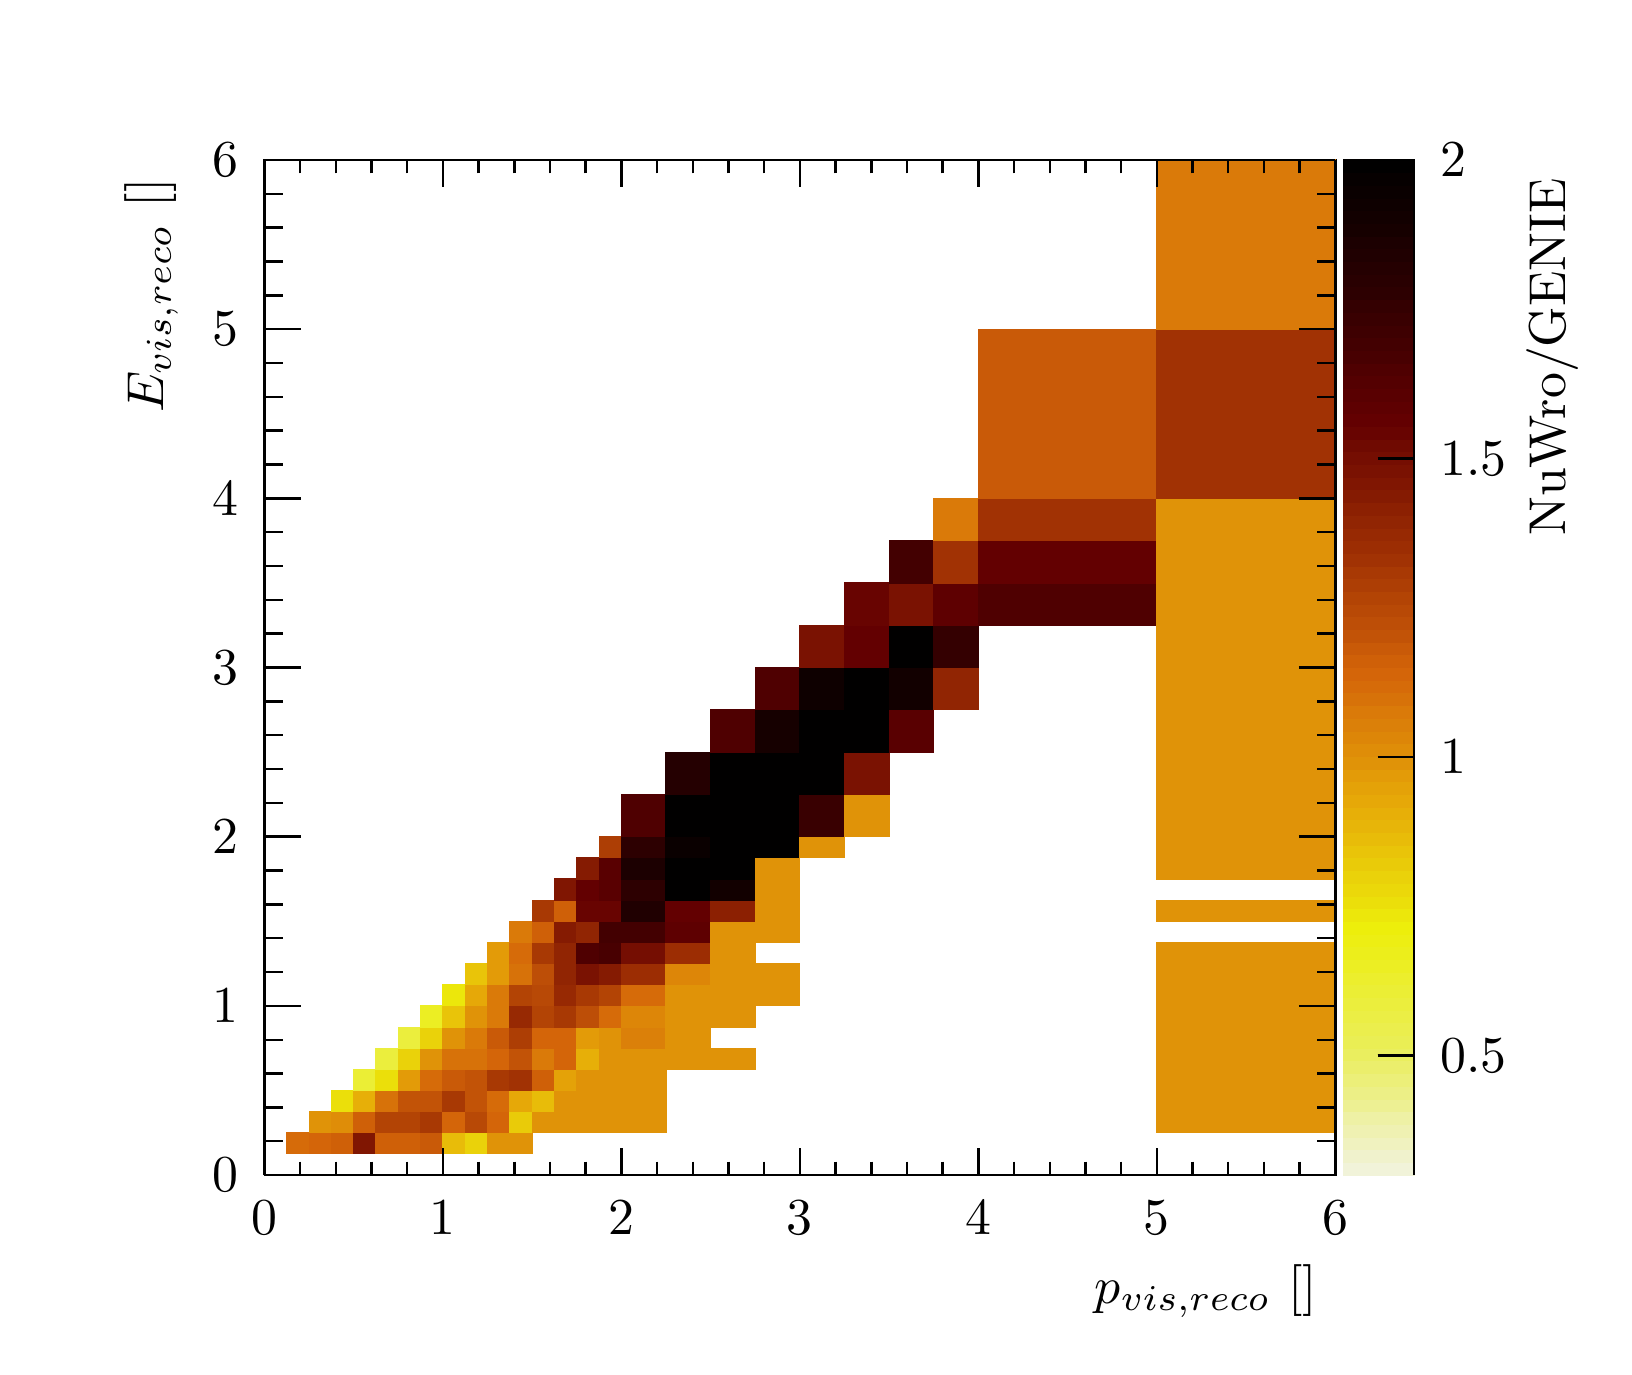
\begin{tikzpicture}
\pgfdeclareplotmark{cross} {
\pgfpathmoveto{\pgfpoint{-0.3\pgfplotmarksize}{\pgfplotmarksize}}
\pgfpathlineto{\pgfpoint{+0.3\pgfplotmarksize}{\pgfplotmarksize}}
\pgfpathlineto{\pgfpoint{+0.3\pgfplotmarksize}{0.3\pgfplotmarksize}}
\pgfpathlineto{\pgfpoint{+1\pgfplotmarksize}{0.3\pgfplotmarksize}}
\pgfpathlineto{\pgfpoint{+1\pgfplotmarksize}{-0.3\pgfplotmarksize}}
\pgfpathlineto{\pgfpoint{+0.3\pgfplotmarksize}{-0.3\pgfplotmarksize}}
\pgfpathlineto{\pgfpoint{+0.3\pgfplotmarksize}{-1.\pgfplotmarksize}}
\pgfpathlineto{\pgfpoint{-0.3\pgfplotmarksize}{-1.\pgfplotmarksize}}
\pgfpathlineto{\pgfpoint{-0.3\pgfplotmarksize}{-0.3\pgfplotmarksize}}
\pgfpathlineto{\pgfpoint{-1.\pgfplotmarksize}{-0.3\pgfplotmarksize}}
\pgfpathlineto{\pgfpoint{-1.\pgfplotmarksize}{0.3\pgfplotmarksize}}
\pgfpathlineto{\pgfpoint{-0.3\pgfplotmarksize}{0.3\pgfplotmarksize}}
\pgfpathclose
\pgfusepathqstroke
}
\pgfdeclareplotmark{cross*} {
\pgfpathmoveto{\pgfpoint{-0.3\pgfplotmarksize}{\pgfplotmarksize}}
\pgfpathlineto{\pgfpoint{+0.3\pgfplotmarksize}{\pgfplotmarksize}}
\pgfpathlineto{\pgfpoint{+0.3\pgfplotmarksize}{0.3\pgfplotmarksize}}
\pgfpathlineto{\pgfpoint{+1\pgfplotmarksize}{0.3\pgfplotmarksize}}
\pgfpathlineto{\pgfpoint{+1\pgfplotmarksize}{-0.3\pgfplotmarksize}}
\pgfpathlineto{\pgfpoint{+0.3\pgfplotmarksize}{-0.3\pgfplotmarksize}}
\pgfpathlineto{\pgfpoint{+0.3\pgfplotmarksize}{-1.\pgfplotmarksize}}
\pgfpathlineto{\pgfpoint{-0.3\pgfplotmarksize}{-1.\pgfplotmarksize}}
\pgfpathlineto{\pgfpoint{-0.3\pgfplotmarksize}{-0.3\pgfplotmarksize}}
\pgfpathlineto{\pgfpoint{-1.\pgfplotmarksize}{-0.3\pgfplotmarksize}}
\pgfpathlineto{\pgfpoint{-1.\pgfplotmarksize}{0.3\pgfplotmarksize}}
\pgfpathlineto{\pgfpoint{-0.3\pgfplotmarksize}{0.3\pgfplotmarksize}}
\pgfpathclose
\pgfusepathqfillstroke
}
\pgfdeclareplotmark{newstar} {
\pgfpathmoveto{\pgfqpoint{0pt}{\pgfplotmarksize}}
\pgfpathlineto{\pgfqpointpolar{44}{0.5\pgfplotmarksize}}
\pgfpathlineto{\pgfqpointpolar{18}{\pgfplotmarksize}}
\pgfpathlineto{\pgfqpointpolar{-20}{0.5\pgfplotmarksize}}
\pgfpathlineto{\pgfqpointpolar{-54}{\pgfplotmarksize}}
\pgfpathlineto{\pgfqpointpolar{-90}{0.5\pgfplotmarksize}}
\pgfpathlineto{\pgfqpointpolar{234}{\pgfplotmarksize}}
\pgfpathlineto{\pgfqpointpolar{198}{0.5\pgfplotmarksize}}
\pgfpathlineto{\pgfqpointpolar{162}{\pgfplotmarksize}}
\pgfpathlineto{\pgfqpointpolar{134}{0.5\pgfplotmarksize}}
\pgfpathclose
\pgfusepathqstroke
}
\pgfdeclareplotmark{newstar*} {
\pgfpathmoveto{\pgfqpoint{0pt}{\pgfplotmarksize}}
\pgfpathlineto{\pgfqpointpolar{44}{0.5\pgfplotmarksize}}
\pgfpathlineto{\pgfqpointpolar{18}{\pgfplotmarksize}}
\pgfpathlineto{\pgfqpointpolar{-20}{0.5\pgfplotmarksize}}
\pgfpathlineto{\pgfqpointpolar{-54}{\pgfplotmarksize}}
\pgfpathlineto{\pgfqpointpolar{-90}{0.5\pgfplotmarksize}}
\pgfpathlineto{\pgfqpointpolar{234}{\pgfplotmarksize}}
\pgfpathlineto{\pgfqpointpolar{198}{0.5\pgfplotmarksize}}
\pgfpathlineto{\pgfqpointpolar{162}{\pgfplotmarksize}}
\pgfpathlineto{\pgfqpointpolar{134}{0.5\pgfplotmarksize}}
\pgfpathclose
\pgfusepathqfillstroke
}
\definecolor{c}{rgb}{1,1,1};
\draw [color=c, fill=c] (0,0) rectangle (20,16.7416);
\draw [color=c, fill=c] (3,2.1764) rectangle (16.6,15.0674);
\definecolor{c}{rgb}{0,0,0};
\draw [c,line width=0.9] (3,2.1764) -- (3,15.0674) -- (16.6,15.0674) -- (16.6,2.1764) -- (3,2.1764);
\definecolor{c}{rgb}{1,1,1};
\draw [color=c, fill=c] (3,2.1764) rectangle (16.6,15.0674);
\definecolor{c}{rgb}{0,0,0};
\draw [c,line width=0.9] (3,2.1764) -- (3,15.0674) -- (16.6,15.0674) -- (16.6,2.1764) -- (3,2.1764);
\definecolor{c}{rgb}{0.83799,0.420711,0.0349265};
\draw [color=c, fill=c] (3.28333,2.44497) rectangle (3.56667,2.71353);
\definecolor{c}{rgb}{0.831373,0.396078,0.0352941};
\draw [color=c, fill=c] (3.56667,2.44497) rectangle (3.85,2.71353);
\definecolor{c}{rgb}{0.810784,0.37549,0.0330882};
\draw [color=c, fill=c] (3.85,2.44497) rectangle (4.13333,2.71353);
\definecolor{c}{rgb}{0.5,0.0882353,0.00784314};
\draw [color=c, fill=c] (4.13333,2.44497) rectangle (4.41667,2.71353);
\definecolor{c}{rgb}{0.810784,0.37549,0.0330882};
\draw [color=c, fill=c] (4.41667,2.44497) rectangle (4.7,2.71353);
\draw [color=c, fill=c] (4.7,2.44497) rectangle (4.98333,2.71353);
\definecolor{c}{rgb}{0.790196,0.354902,0.0308824};
\draw [color=c, fill=c] (4.98333,2.44497) rectangle (5.26667,2.71353);
\definecolor{c}{rgb}{0.909681,0.736029,0.0346814};
\draw [color=c, fill=c] (5.26667,2.44497) rectangle (5.55,2.71353);
\definecolor{c}{rgb}{0.91826,0.821814,0.0383578};
\draw [color=c, fill=c] (5.55,2.44497) rectangle (5.83333,2.71353);
\definecolor{c}{rgb}{0.879902,0.576716,0.032598};
\draw [color=c, fill=c] (5.83333,2.44497) rectangle (6.11667,2.71353);
\draw [color=c, fill=c] (6.11667,2.44497) rectangle (6.4,2.71353);
\draw [color=c, fill=c] (3.56667,2.71353) rectangle (3.85,2.98209);
\definecolor{c}{rgb}{0.873284,0.552083,0.0329657};
\draw [color=c, fill=c] (3.85,2.71353) rectangle (4.13333,2.98209);
\definecolor{c}{rgb}{0.810784,0.37549,0.0330882};
\draw [color=c, fill=c] (4.13333,2.71353) rectangle (4.41667,2.98209);
\definecolor{c}{rgb}{0.70098,0.265686,0.0213235};
\draw [color=c, fill=c] (4.41667,2.71353) rectangle (4.7,2.98209);
\draw [color=c, fill=c] (4.7,2.71353) rectangle (4.98333,2.98209);
\definecolor{c}{rgb}{0.659804,0.22451,0.0169118};
\draw [color=c, fill=c] (4.98333,2.71353) rectangle (5.26667,2.98209);
\definecolor{c}{rgb}{0.831373,0.396078,0.0352941};
\draw [color=c, fill=c] (5.26667,2.71353) rectangle (5.55,2.98209);
\definecolor{c}{rgb}{0.721569,0.286275,0.0235294};
\draw [color=c, fill=c] (5.55,2.71353) rectangle (5.83333,2.98209);
\definecolor{c}{rgb}{0.831373,0.396078,0.0352941};
\draw [color=c, fill=c] (5.83333,2.71353) rectangle (6.11667,2.98209);
\definecolor{c}{rgb}{0.915686,0.796078,0.0372549};
\draw [color=c, fill=c] (6.11667,2.71353) rectangle (6.4,2.98209);
\definecolor{c}{rgb}{0.879902,0.576716,0.032598};
\draw [color=c, fill=c] (6.4,2.71353) rectangle (6.68333,2.98209);
\draw [color=c, fill=c] (6.68333,2.71353) rectangle (6.96667,2.98209);
\draw [color=c, fill=c] (6.96667,2.71353) rectangle (7.25,2.98209);
\draw [color=c, fill=c] (7.25,2.71353) rectangle (7.53333,2.98209);
\draw [color=c, fill=c] (7.53333,2.71353) rectangle (8.1,2.98209);
\draw [color=c, fill=c] (14.3333,2.71353) rectangle (16.6,2.98209);
\definecolor{c}{rgb}{0.923407,0.873284,0.0405637};
\draw [color=c, fill=c] (3.85,2.98209) rectangle (4.13333,3.25066);
\definecolor{c}{rgb}{0.904534,0.684559,0.0324755};
\draw [color=c, fill=c] (4.13333,2.98209) rectangle (4.41667,3.25066);
\definecolor{c}{rgb}{0.844608,0.445343,0.0345588};
\draw [color=c, fill=c] (4.41667,2.98209) rectangle (4.7,3.25066);
\definecolor{c}{rgb}{0.762745,0.327451,0.0279412};
\draw [color=c, fill=c] (4.7,2.98209) rectangle (4.98333,3.25066);
\draw [color=c, fill=c] (4.98333,2.98209) rectangle (5.26667,3.25066);
\definecolor{c}{rgb}{0.659804,0.22451,0.0169118};
\draw [color=c, fill=c] (5.26667,2.98209) rectangle (5.55,3.25066);
\definecolor{c}{rgb}{0.762745,0.327451,0.0279412};
\draw [color=c, fill=c] (5.55,2.98209) rectangle (5.83333,3.25066);
\definecolor{c}{rgb}{0.83799,0.420711,0.0349265};
\draw [color=c, fill=c] (5.83333,2.98209) rectangle (6.11667,3.25066);
\definecolor{c}{rgb}{0.901961,0.658824,0.0313726};
\draw [color=c, fill=c] (6.11667,2.98209) rectangle (6.4,3.25066);
\definecolor{c}{rgb}{0.909681,0.736029,0.0346814};
\draw [color=c, fill=c] (6.4,2.98209) rectangle (6.68333,3.25066);
\definecolor{c}{rgb}{0.879902,0.576716,0.032598};
\draw [color=c, fill=c] (6.68333,2.98209) rectangle (6.96667,3.25066);
\draw [color=c, fill=c] (6.96667,2.98209) rectangle (7.25,3.25066);
\draw [color=c, fill=c] (7.25,2.98209) rectangle (7.53333,3.25066);
\draw [color=c, fill=c] (7.53333,2.98209) rectangle (8.1,3.25066);
\draw [color=c, fill=c] (14.3333,2.98209) rectangle (16.6,3.25066);
\definecolor{c}{rgb}{0.923529,0.933333,0.207843};
\draw [color=c, fill=c] (4.13333,3.25066) rectangle (4.41667,3.51922);
\definecolor{c}{rgb}{0.923407,0.873284,0.0405637};
\draw [color=c, fill=c] (4.41667,3.25066) rectangle (4.7,3.51922);
\definecolor{c}{rgb}{0.888726,0.609559,0.0321078};
\draw [color=c, fill=c] (4.7,3.25066) rectangle (4.98333,3.51922);
\definecolor{c}{rgb}{0.83799,0.420711,0.0349265};
\draw [color=c, fill=c] (4.98333,3.25066) rectangle (5.26667,3.51922);
\definecolor{c}{rgb}{0.790196,0.354902,0.0308824};
\draw [color=c, fill=c] (5.26667,3.25066) rectangle (5.55,3.51922);
\definecolor{c}{rgb}{0.762745,0.327451,0.0279412};
\draw [color=c, fill=c] (5.55,3.25066) rectangle (5.83333,3.51922);
\definecolor{c}{rgb}{0.659804,0.22451,0.0169118};
\draw [color=c, fill=c] (5.83333,3.25066) rectangle (6.11667,3.51922);
\definecolor{c}{rgb}{0.632353,0.197059,0.0139706};
\draw [color=c, fill=c] (6.11667,3.25066) rectangle (6.4,3.51922);
\definecolor{c}{rgb}{0.810784,0.37549,0.0330882};
\draw [color=c, fill=c] (6.4,3.25066) rectangle (6.68333,3.51922);
\definecolor{c}{rgb}{0.895343,0.634191,0.0317402};
\draw [color=c, fill=c] (6.68333,3.25066) rectangle (6.96667,3.51922);
\definecolor{c}{rgb}{0.879902,0.576716,0.032598};
\draw [color=c, fill=c] (6.96667,3.25066) rectangle (7.25,3.51922);
\draw [color=c, fill=c] (7.25,3.25066) rectangle (7.53333,3.51922);
\draw [color=c, fill=c] (7.53333,3.25066) rectangle (8.1,3.51922);
\draw [color=c, fill=c] (14.3333,3.25066) rectangle (16.6,3.51922);
\definecolor{c}{rgb}{0.922426,0.933333,0.238725};
\draw [color=c, fill=c] (4.41667,3.51922) rectangle (4.7,3.78778);
\definecolor{c}{rgb}{0.91826,0.821814,0.0383578};
\draw [color=c, fill=c] (4.7,3.51922) rectangle (4.98333,3.78778);
\definecolor{c}{rgb}{0.879902,0.576716,0.032598};
\draw [color=c, fill=c] (4.98333,3.51922) rectangle (5.26667,3.78778);
\definecolor{c}{rgb}{0.844608,0.445343,0.0345588};
\draw [color=c, fill=c] (5.26667,3.51922) rectangle (5.55,3.78778);
\draw [color=c, fill=c] (5.55,3.51922) rectangle (5.83333,3.78778);
\definecolor{c}{rgb}{0.831373,0.396078,0.0352941};
\draw [color=c, fill=c] (5.83333,3.51922) rectangle (6.11667,3.78778);
\definecolor{c}{rgb}{0.762745,0.327451,0.0279412};
\draw [color=c, fill=c] (6.11667,3.51922) rectangle (6.4,3.78778);
\definecolor{c}{rgb}{0.853431,0.478186,0.0340686};
\draw [color=c, fill=c] (6.4,3.51922) rectangle (6.68333,3.78778);
\definecolor{c}{rgb}{0.831373,0.396078,0.0352941};
\draw [color=c, fill=c] (6.68333,3.51922) rectangle (6.96667,3.78778);
\definecolor{c}{rgb}{0.904534,0.684559,0.0324755};
\draw [color=c, fill=c] (6.96667,3.51922) rectangle (7.25,3.78778);
\definecolor{c}{rgb}{0.879902,0.576716,0.032598};
\draw [color=c, fill=c] (7.25,3.51922) rectangle (7.53333,3.78778);
\draw [color=c, fill=c] (7.53333,3.51922) rectangle (8.1,3.78778);
\draw [color=c, fill=c] (8.1,3.51922) rectangle (8.66667,3.78778);
\draw [color=c, fill=c] (8.66667,3.51922) rectangle (9.23333,3.78778);
\draw [color=c, fill=c] (14.3333,3.51922) rectangle (16.6,3.78778);
\definecolor{c}{rgb}{0.922426,0.933333,0.238725};
\draw [color=c, fill=c] (4.7,3.78778) rectangle (4.98333,4.05634);
\definecolor{c}{rgb}{0.91826,0.821814,0.0383578};
\draw [color=c, fill=c] (4.98333,3.78778) rectangle (5.26667,4.05634);
\definecolor{c}{rgb}{0.879902,0.576716,0.032598};
\draw [color=c, fill=c] (5.26667,3.78778) rectangle (5.55,4.05634);
\definecolor{c}{rgb}{0.853431,0.478186,0.0340686};
\draw [color=c, fill=c] (5.55,3.78778) rectangle (5.83333,4.05634);
\definecolor{c}{rgb}{0.790196,0.354902,0.0308824};
\draw [color=c, fill=c] (5.83333,3.78778) rectangle (6.11667,4.05634);
\definecolor{c}{rgb}{0.680392,0.245098,0.0191176};
\draw [color=c, fill=c] (6.11667,3.78778) rectangle (6.4,4.05634);
\definecolor{c}{rgb}{0.831373,0.396078,0.0352941};
\draw [color=c, fill=c] (6.4,3.78778) rectangle (6.68333,4.05634);
\draw [color=c, fill=c] (6.68333,3.78778) rectangle (6.96667,4.05634);
\definecolor{c}{rgb}{0.888726,0.609559,0.0321078};
\draw [color=c, fill=c] (6.96667,3.78778) rectangle (7.25,4.05634);
\definecolor{c}{rgb}{0.879902,0.576716,0.032598};
\draw [color=c, fill=c] (7.25,3.78778) rectangle (7.53333,4.05634);
\definecolor{c}{rgb}{0.860049,0.502819,0.033701};
\draw [color=c, fill=c] (7.53333,3.78778) rectangle (8.1,4.05634);
\definecolor{c}{rgb}{0.879902,0.576716,0.032598};
\draw [color=c, fill=c] (8.1,3.78778) rectangle (8.66667,4.05634);
\draw [color=c, fill=c] (14.3333,3.78778) rectangle (16.6,4.05634);
\definecolor{c}{rgb}{0.926103,0.933333,0.135784};
\draw [color=c, fill=c] (4.98333,4.05634) rectangle (5.26667,4.32491);
\definecolor{c}{rgb}{0.913113,0.770343,0.036152};
\draw [color=c, fill=c] (5.26667,4.05634) rectangle (5.55,4.32491);
\definecolor{c}{rgb}{0.879902,0.576716,0.032598};
\draw [color=c, fill=c] (5.55,4.05634) rectangle (5.83333,4.32491);
\definecolor{c}{rgb}{0.853431,0.478186,0.0340686};
\draw [color=c, fill=c] (5.83333,4.05634) rectangle (6.11667,4.32491);
\definecolor{c}{rgb}{0.590809,0.159926,0.0110294};
\draw [color=c, fill=c] (6.11667,4.05634) rectangle (6.4,4.32491);
\definecolor{c}{rgb}{0.70098,0.265686,0.0213235};
\draw [color=c, fill=c] (6.4,4.05634) rectangle (6.68333,4.32491);
\definecolor{c}{rgb}{0.659804,0.22451,0.0169118};
\draw [color=c, fill=c] (6.68333,4.05634) rectangle (6.96667,4.32491);
\definecolor{c}{rgb}{0.742157,0.306863,0.0257353};
\draw [color=c, fill=c] (6.96667,4.05634) rectangle (7.25,4.32491);
\definecolor{c}{rgb}{0.83799,0.420711,0.0349265};
\draw [color=c, fill=c] (7.25,4.05634) rectangle (7.53333,4.32491);
\definecolor{c}{rgb}{0.866667,0.527451,0.0333333};
\draw [color=c, fill=c] (7.53333,4.05634) rectangle (8.1,4.32491);
\definecolor{c}{rgb}{0.879902,0.576716,0.032598};
\draw [color=c, fill=c] (8.1,4.05634) rectangle (8.66667,4.32491);
\draw [color=c, fill=c] (8.66667,4.05634) rectangle (9.23333,4.32491);
\draw [color=c, fill=c] (14.3333,4.05634) rectangle (16.6,4.32491);
\definecolor{c}{rgb}{0.926838,0.907598,0.0420343};
\draw [color=c, fill=c] (5.26667,4.32491) rectangle (5.55,4.59347);
\definecolor{c}{rgb}{0.901961,0.658824,0.0313726};
\draw [color=c, fill=c] (5.55,4.32491) rectangle (5.83333,4.59347);
\definecolor{c}{rgb}{0.853431,0.478186,0.0340686};
\draw [color=c, fill=c] (5.83333,4.32491) rectangle (6.11667,4.59347);
\definecolor{c}{rgb}{0.70098,0.265686,0.0213235};
\draw [color=c, fill=c] (6.11667,4.32491) rectangle (6.4,4.59347);
\definecolor{c}{rgb}{0.721569,0.286275,0.0235294};
\draw [color=c, fill=c] (6.4,4.32491) rectangle (6.68333,4.59347);
\definecolor{c}{rgb}{0.590809,0.159926,0.0110294};
\draw [color=c, fill=c] (6.68333,4.32491) rectangle (6.96667,4.59347);
\definecolor{c}{rgb}{0.659804,0.22451,0.0169118};
\draw [color=c, fill=c] (6.96667,4.32491) rectangle (7.25,4.59347);
\definecolor{c}{rgb}{0.70098,0.265686,0.0213235};
\draw [color=c, fill=c] (7.25,4.32491) rectangle (7.53333,4.59347);
\definecolor{c}{rgb}{0.83799,0.420711,0.0349265};
\draw [color=c, fill=c] (7.53333,4.32491) rectangle (8.1,4.59347);
\definecolor{c}{rgb}{0.879902,0.576716,0.032598};
\draw [color=c, fill=c] (8.1,4.32491) rectangle (8.66667,4.59347);
\draw [color=c, fill=c] (8.66667,4.32491) rectangle (9.23333,4.59347);
\draw [color=c, fill=c] (9.23333,4.32491) rectangle (9.8,4.59347);
\draw [color=c, fill=c] (14.3333,4.32491) rectangle (16.6,4.59347);
\definecolor{c}{rgb}{0.913113,0.770343,0.036152};
\draw [color=c, fill=c] (5.55,4.59347) rectangle (5.83333,4.86203);
\definecolor{c}{rgb}{0.888726,0.609559,0.0321078};
\draw [color=c, fill=c] (5.83333,4.59347) rectangle (6.11667,4.86203);
\definecolor{c}{rgb}{0.844608,0.445343,0.0345588};
\draw [color=c, fill=c] (6.11667,4.59347) rectangle (6.4,4.86203);
\definecolor{c}{rgb}{0.742157,0.306863,0.0257353};
\draw [color=c, fill=c] (6.4,4.59347) rectangle (6.68333,4.86203);
\definecolor{c}{rgb}{0.569853,0.143382,0.0102941};
\draw [color=c, fill=c] (6.68333,4.59347) rectangle (6.96667,4.86203);
\definecolor{c}{rgb}{0.479044,0.0716912,0.00710784};
\draw [color=c, fill=c] (6.96667,4.59347) rectangle (7.25,4.86203);
\definecolor{c}{rgb}{0.520956,0.104779,0.00857843};
\draw [color=c, fill=c] (7.25,4.59347) rectangle (7.53333,4.86203);
\definecolor{c}{rgb}{0.611765,0.176471,0.0117647};
\draw [color=c, fill=c] (7.53333,4.59347) rectangle (8.1,4.86203);
\definecolor{c}{rgb}{0.866667,0.527451,0.0333333};
\draw [color=c, fill=c] (8.1,4.59347) rectangle (8.66667,4.86203);
\definecolor{c}{rgb}{0.879902,0.576716,0.032598};
\draw [color=c, fill=c] (8.66667,4.59347) rectangle (9.23333,4.86203);
\draw [color=c, fill=c] (9.23333,4.59347) rectangle (9.8,4.86203);
\draw [color=c, fill=c] (14.3333,4.59347) rectangle (16.6,4.86203);
\definecolor{c}{rgb}{0.888726,0.609559,0.0321078};
\draw [color=c, fill=c] (5.83333,4.86203) rectangle (6.11667,5.13059);
\definecolor{c}{rgb}{0.83799,0.420711,0.0349265};
\draw [color=c, fill=c] (6.11667,4.86203) rectangle (6.4,5.13059);
\definecolor{c}{rgb}{0.659804,0.22451,0.0169118};
\draw [color=c, fill=c] (6.4,4.86203) rectangle (6.68333,5.13059);
\definecolor{c}{rgb}{0.569853,0.143382,0.0102941};
\draw [color=c, fill=c] (6.68333,4.86203) rectangle (6.96667,5.13059);
\definecolor{c}{rgb}{0.308824,0,0.00392157};
\draw [color=c, fill=c] (6.96667,4.86203) rectangle (7.25,5.13059);
\definecolor{c}{rgb}{0.282353,0,0.00392157};
\draw [color=c, fill=c] (7.25,4.86203) rectangle (7.53333,5.13059);
\definecolor{c}{rgb}{0.458088,0.0551471,0.00637255};
\draw [color=c, fill=c] (7.53333,4.86203) rectangle (8.1,5.13059);
\definecolor{c}{rgb}{0.611765,0.176471,0.0117647};
\draw [color=c, fill=c] (8.1,4.86203) rectangle (8.66667,5.13059);
\definecolor{c}{rgb}{0.879902,0.576716,0.032598};
\draw [color=c, fill=c] (8.66667,4.86203) rectangle (9.23333,5.13059);
\draw [color=c, fill=c] (14.3333,4.86203) rectangle (16.6,5.13059);
\definecolor{c}{rgb}{0.853431,0.478186,0.0340686};
\draw [color=c, fill=c] (6.11667,5.13059) rectangle (6.4,5.39916);
\definecolor{c}{rgb}{0.810784,0.37549,0.0330882};
\draw [color=c, fill=c] (6.4,5.13059) rectangle (6.68333,5.39916);
\definecolor{c}{rgb}{0.520956,0.104779,0.00857843};
\draw [color=c, fill=c] (6.68333,5.13059) rectangle (6.96667,5.39916);
\definecolor{c}{rgb}{0.569853,0.143382,0.0102941};
\draw [color=c, fill=c] (6.96667,5.13059) rectangle (7.25,5.39916);
\definecolor{c}{rgb}{0.2625,0,0.00392157};
\draw [color=c, fill=c] (7.25,5.13059) rectangle (7.53333,5.39916);
\draw [color=c, fill=c] (7.53333,5.13059) rectangle (8.1,5.39916);
\definecolor{c}{rgb}{0.368382,0,0.00392157};
\draw [color=c, fill=c] (8.1,5.13059) rectangle (8.66667,5.39916);
\definecolor{c}{rgb}{0.879902,0.576716,0.032598};
\draw [color=c, fill=c] (8.66667,5.13059) rectangle (9.23333,5.39916);
\draw [color=c, fill=c] (9.23333,5.13059) rectangle (9.8,5.39916);
\definecolor{c}{rgb}{0.659804,0.22451,0.0169118};
\draw [color=c, fill=c] (6.4,5.39916) rectangle (6.68333,5.66772);
\definecolor{c}{rgb}{0.810784,0.37549,0.0330882};
\draw [color=c, fill=c] (6.68333,5.39916) rectangle (6.96667,5.66772);
\definecolor{c}{rgb}{0.409191,0.0165441,0.00465686};
\draw [color=c, fill=c] (6.96667,5.39916) rectangle (7.25,5.66772);
\draw [color=c, fill=c] (7.25,5.39916) rectangle (7.53333,5.66772);
\definecolor{c}{rgb}{0.126838,0,0.00281863};
\draw [color=c, fill=c] (7.53333,5.39916) rectangle (8.1,5.66772);
\definecolor{c}{rgb}{0.388235,0,0.00392157};
\draw [color=c, fill=c] (8.1,5.39916) rectangle (8.66667,5.66772);
\definecolor{c}{rgb}{0.548897,0.126838,0.00955882};
\draw [color=c, fill=c] (8.66667,5.39916) rectangle (9.23333,5.66772);
\definecolor{c}{rgb}{0.879902,0.576716,0.032598};
\draw [color=c, fill=c] (9.23333,5.39916) rectangle (9.8,5.66772);
\draw [color=c, fill=c] (14.3333,5.39916) rectangle (16.6,5.66772);
\definecolor{c}{rgb}{0.5,0.0882353,0.00784314};
\draw [color=c, fill=c] (6.68333,5.66772) rectangle (6.96667,5.93628);
\definecolor{c}{rgb}{0.388235,0,0.00392157};
\draw [color=c, fill=c] (6.96667,5.66772) rectangle (7.25,5.93628);
\definecolor{c}{rgb}{0.348529,0,0.00392157};
\draw [color=c, fill=c] (7.25,5.66772) rectangle (7.53333,5.93628);
\definecolor{c}{rgb}{0.176471,0,0.00392157};
\draw [color=c, fill=c] (7.53333,5.66772) rectangle (8.1,5.93628);
\definecolor{c}{rgb}{0.00551471,0,0.000122549};
\draw [color=c, fill=c] (8.1,5.66772) rectangle (8.66667,5.93628);
\definecolor{c}{rgb}{0.0716912,0,0.00159314};
\draw [color=c, fill=c] (8.66667,5.66772) rectangle (9.23333,5.93628);
\definecolor{c}{rgb}{0.879902,0.576716,0.032598};
\draw [color=c, fill=c] (9.23333,5.66772) rectangle (9.8,5.93628);
\definecolor{c}{rgb}{0.520956,0.104779,0.00857843};
\draw [color=c, fill=c] (6.96667,5.93628) rectangle (7.25,6.20485);
\definecolor{c}{rgb}{0.348529,0,0.00392157};
\draw [color=c, fill=c] (7.25,5.93628) rectangle (7.53333,6.20485);
\definecolor{c}{rgb}{0.110294,0,0.00245098};
\draw [color=c, fill=c] (7.53333,5.93628) rectangle (8.1,6.20485);
\definecolor{c}{rgb}{0.00551471,0,0.000122549};
\draw [color=c, fill=c] (8.1,5.93628) rectangle (8.66667,6.20485);
\draw [color=c, fill=c] (8.66667,5.93628) rectangle (9.23333,6.20485);
\definecolor{c}{rgb}{0.879902,0.576716,0.032598};
\draw [color=c, fill=c] (9.23333,5.93628) rectangle (9.8,6.20485);
\draw [color=c, fill=c] (14.3333,5.93628) rectangle (16.6,6.20485);
\definecolor{c}{rgb}{0.680392,0.245098,0.0191176};
\draw [color=c, fill=c] (7.25,6.20485) rectangle (7.53333,6.47341);
\definecolor{c}{rgb}{0.176471,0,0.00392157};
\draw [color=c, fill=c] (7.53333,6.20485) rectangle (8.1,6.47341);
\definecolor{c}{rgb}{0.0386029,0,0.000857843};
\draw [color=c, fill=c] (8.1,6.20485) rectangle (8.66667,6.47341);
\definecolor{c}{rgb}{0.00551471,0,0.000122549};
\draw [color=c, fill=c] (8.66667,6.20485) rectangle (9.23333,6.47341);
\draw [color=c, fill=c] (9.23333,6.20485) rectangle (9.8,6.47341);
\definecolor{c}{rgb}{0.879902,0.576716,0.032598};
\draw [color=c, fill=c] (9.8,6.20485) rectangle (10.3667,6.47341);
\draw [color=c, fill=c] (14.3333,6.20485) rectangle (16.6,6.47341);
\definecolor{c}{rgb}{0.308824,0,0.00392157};
\draw [color=c, fill=c] (7.53333,6.47341) rectangle (8.1,7.01053);
\definecolor{c}{rgb}{0.00551471,0,0.000122549};
\draw [color=c, fill=c] (8.1,6.47341) rectangle (8.66667,7.01053);
\draw [color=c, fill=c] (8.66667,6.47341) rectangle (9.23333,7.01053);
\draw [color=c, fill=c] (9.23333,6.47341) rectangle (9.8,7.01053);
\definecolor{c}{rgb}{0.222794,0,0.00392157};
\draw [color=c, fill=c] (9.8,6.47341) rectangle (10.3667,7.01053);
\definecolor{c}{rgb}{0.879902,0.576716,0.032598};
\draw [color=c, fill=c] (10.3667,6.47341) rectangle (10.9333,7.01053);
\draw [color=c, fill=c] (14.3333,6.47341) rectangle (16.6,7.01053);
\definecolor{c}{rgb}{0.143382,0,0.00318627};
\draw [color=c, fill=c] (8.1,7.01053) rectangle (8.66667,7.54766);
\definecolor{c}{rgb}{0.00551471,0,0.000122549};
\draw [color=c, fill=c] (8.66667,7.01053) rectangle (9.23333,7.54766);
\draw [color=c, fill=c] (9.23333,7.01053) rectangle (9.8,7.54766);
\draw [color=c, fill=c] (9.8,7.01053) rectangle (10.3667,7.54766);
\definecolor{c}{rgb}{0.479044,0.0716912,0.00710784};
\draw [color=c, fill=c] (10.3667,7.01053) rectangle (10.9333,7.54766);
\definecolor{c}{rgb}{0.879902,0.576716,0.032598};
\draw [color=c, fill=c] (14.3333,7.01053) rectangle (16.6,7.54766);
\definecolor{c}{rgb}{0.308824,0,0.00392157};
\draw [color=c, fill=c] (8.66667,7.54766) rectangle (9.23333,8.08478);
\definecolor{c}{rgb}{0.0882353,0,0.00196078};
\draw [color=c, fill=c] (9.23333,7.54766) rectangle (9.8,8.08478);
\definecolor{c}{rgb}{0.00551471,0,0.000122549};
\draw [color=c, fill=c] (9.8,7.54766) rectangle (10.3667,8.08478);
\draw [color=c, fill=c] (10.3667,7.54766) rectangle (10.9333,8.08478);
\definecolor{c}{rgb}{0.348529,0,0.00392157};
\draw [color=c, fill=c] (10.9333,7.54766) rectangle (11.5,8.08478);
\definecolor{c}{rgb}{0.879902,0.576716,0.032598};
\draw [color=c, fill=c] (14.3333,7.54766) rectangle (16.6,8.08478);
\definecolor{c}{rgb}{0.308824,0,0.00392157};
\draw [color=c, fill=c] (9.23333,8.08478) rectangle (9.8,8.62191);
\definecolor{c}{rgb}{0.0551471,0,0.00122549};
\draw [color=c, fill=c] (9.8,8.08478) rectangle (10.3667,8.62191);
\definecolor{c}{rgb}{0.00551471,0,0.000122549};
\draw [color=c, fill=c] (10.3667,8.08478) rectangle (10.9333,8.62191);
\definecolor{c}{rgb}{0.0716912,0,0.00159314};
\draw [color=c, fill=c] (10.9333,8.08478) rectangle (11.5,8.62191);
\definecolor{c}{rgb}{0.569853,0.143382,0.0102941};
\draw [color=c, fill=c] (11.5,8.08478) rectangle (12.0667,8.62191);
\definecolor{c}{rgb}{0.879902,0.576716,0.032598};
\draw [color=c, fill=c] (14.3333,8.08478) rectangle (16.6,8.62191);
\definecolor{c}{rgb}{0.479044,0.0716912,0.00710784};
\draw [color=c, fill=c] (9.8,8.62191) rectangle (10.3667,9.15904);
\definecolor{c}{rgb}{0.388235,0,0.00392157};
\draw [color=c, fill=c] (10.3667,8.62191) rectangle (10.9333,9.15904);
\definecolor{c}{rgb}{0.00551471,0,0.000122549};
\draw [color=c, fill=c] (10.9333,8.62191) rectangle (11.5,9.15904);
\definecolor{c}{rgb}{0.202941,0,0.00392157};
\draw [color=c, fill=c] (11.5,8.62191) rectangle (12.0667,9.15904);
\definecolor{c}{rgb}{0.879902,0.576716,0.032598};
\draw [color=c, fill=c] (14.3333,8.62191) rectangle (16.6,9.15904);
\definecolor{c}{rgb}{0.409191,0.0165441,0.00465686};
\draw [color=c, fill=c] (10.3667,9.15904) rectangle (10.9333,9.69616);
\definecolor{c}{rgb}{0.479044,0.0716912,0.00710784};
\draw [color=c, fill=c] (10.9333,9.15904) rectangle (11.5,9.69616);
\definecolor{c}{rgb}{0.368382,0,0.00392157};
\draw [color=c, fill=c] (11.5,9.15904) rectangle (12.0667,9.69616);
\definecolor{c}{rgb}{0.308824,0,0.00392157};
\draw [color=c, fill=c] (12.0667,9.15904) rectangle (14.3333,9.69616);
\definecolor{c}{rgb}{0.879902,0.576716,0.032598};
\draw [color=c, fill=c] (14.3333,9.15904) rectangle (16.6,9.69616);
\definecolor{c}{rgb}{0.2625,0,0.00392157};
\draw [color=c, fill=c] (10.9333,9.69616) rectangle (11.5,10.2333);
\definecolor{c}{rgb}{0.632353,0.197059,0.0139706};
\draw [color=c, fill=c] (11.5,9.69616) rectangle (12.0667,10.2333);
\definecolor{c}{rgb}{0.388235,0,0.00392157};
\draw [color=c, fill=c] (12.0667,9.69616) rectangle (14.3333,10.2333);
\definecolor{c}{rgb}{0.879902,0.576716,0.032598};
\draw [color=c, fill=c] (14.3333,9.69616) rectangle (16.6,10.2333);
\definecolor{c}{rgb}{0.853431,0.478186,0.0340686};
\draw [color=c, fill=c] (11.5,10.2333) rectangle (12.0667,10.7704);
\definecolor{c}{rgb}{0.632353,0.197059,0.0139706};
\draw [color=c, fill=c] (12.0667,10.2333) rectangle (14.3333,10.7704);
\definecolor{c}{rgb}{0.879902,0.576716,0.032598};
\draw [color=c, fill=c] (14.3333,10.2333) rectangle (16.6,10.7704);
\definecolor{c}{rgb}{0.790196,0.354902,0.0308824};
\draw [color=c, fill=c] (12.0667,10.7704) rectangle (14.3333,12.9189);
\definecolor{c}{rgb}{0.632353,0.197059,0.0139706};
\draw [color=c, fill=c] (14.3333,10.7704) rectangle (16.6,12.9189);
\definecolor{c}{rgb}{0.853431,0.478186,0.0340686};
\draw [color=c, fill=c] (14.3333,12.9189) rectangle (16.6,15.0674);
\definecolor{c}{rgb}{0,0,0};
\draw [c,line width=0.9] (3,2.1764) -- (16.6,2.1764);
\draw [c,line width=0.9] (3,2.51793) -- (3,2.1764);
\draw [c,line width=0.9] (3.45333,2.34717) -- (3.45333,2.1764);
\draw [c,line width=0.9] (3.90667,2.34717) -- (3.90667,2.1764);
\draw [c,line width=0.9] (4.36,2.34717) -- (4.36,2.1764);
\draw [c,line width=0.9] (4.81333,2.34717) -- (4.81333,2.1764);
\draw [c,line width=0.9] (5.26667,2.51793) -- (5.26667,2.1764);
\draw [c,line width=0.9] (5.72,2.34717) -- (5.72,2.1764);
\draw [c,line width=0.9] (6.17333,2.34717) -- (6.17333,2.1764);
\draw [c,line width=0.9] (6.62667,2.34717) -- (6.62667,2.1764);
\draw [c,line width=0.9] (7.08,2.34717) -- (7.08,2.1764);
\draw [c,line width=0.9] (7.53333,2.51793) -- (7.53333,2.1764);
\draw [c,line width=0.9] (7.98667,2.34717) -- (7.98667,2.1764);
\draw [c,line width=0.9] (8.44,2.34717) -- (8.44,2.1764);
\draw [c,line width=0.9] (8.89333,2.34717) -- (8.89333,2.1764);
\draw [c,line width=0.9] (9.34667,2.34717) -- (9.34667,2.1764);
\draw [c,line width=0.9] (9.8,2.51793) -- (9.8,2.1764);
\draw [c,line width=0.9] (10.2533,2.34717) -- (10.2533,2.1764);
\draw [c,line width=0.9] (10.7067,2.34717) -- (10.7067,2.1764);
\draw [c,line width=0.9] (11.16,2.34717) -- (11.16,2.1764);
\draw [c,line width=0.9] (11.6133,2.34717) -- (11.6133,2.1764);
\draw [c,line width=0.9] (12.0667,2.51793) -- (12.0667,2.1764);
\draw [c,line width=0.9] (12.52,2.34717) -- (12.52,2.1764);
\draw [c,line width=0.9] (12.9733,2.34717) -- (12.9733,2.1764);
\draw [c,line width=0.9] (13.4267,2.34717) -- (13.4267,2.1764);
\draw [c,line width=0.9] (13.88,2.34717) -- (13.88,2.1764);
\draw [c,line width=0.9] (14.3333,2.51793) -- (14.3333,2.1764);
\draw [c,line width=0.9] (14.7867,2.34717) -- (14.7867,2.1764);
\draw [c,line width=0.9] (15.24,2.34717) -- (15.24,2.1764);
\draw [c,line width=0.9] (15.6933,2.34717) -- (15.6933,2.1764);
\draw [c,line width=0.9] (16.1467,2.34717) -- (16.1467,2.1764);
\draw [c,line width=0.9] (16.6,2.51793) -- (16.6,2.1764);
\draw [anchor=base] (3,1.42303) node[scale=1.8716, color=c, rotate=0]{0};
\draw [anchor=base] (5.26667,1.42303) node[scale=1.8716, color=c, rotate=0]{1};
\draw [anchor=base] (7.53333,1.42303) node[scale=1.8716, color=c, rotate=0]{2};
\draw [anchor=base] (9.8,1.42303) node[scale=1.8716, color=c, rotate=0]{3};
\draw [anchor=base] (12.0667,1.42303) node[scale=1.8716, color=c, rotate=0]{4};
\draw [anchor=base] (14.3333,1.42303) node[scale=1.8716, color=c, rotate=0]{5};
\draw [anchor=base] (16.6,1.42303) node[scale=1.8716, color=c, rotate=0]{6};
\draw [anchor= east] (16.6,0.703146) node[scale=1.8716, color=c, rotate=0]{$ p_{\text{vis, reco}}$ [\si{\GeV\per\clight}] };
\draw [c,line width=0.9] (3,15.0674) -- (16.6,15.0674);
\draw [c,line width=0.9] (3,14.7259) -- (3,15.0674);
\draw [c,line width=0.9] (3.45333,14.8967) -- (3.45333,15.0674);
\draw [c,line width=0.9] (3.90667,14.8967) -- (3.90667,15.0674);
\draw [c,line width=0.9] (4.36,14.8967) -- (4.36,15.0674);
\draw [c,line width=0.9] (4.81333,14.8967) -- (4.81333,15.0674);
\draw [c,line width=0.9] (5.26667,14.7259) -- (5.26667,15.0674);
\draw [c,line width=0.9] (5.72,14.8967) -- (5.72,15.0674);
\draw [c,line width=0.9] (6.17333,14.8967) -- (6.17333,15.0674);
\draw [c,line width=0.9] (6.62667,14.8967) -- (6.62667,15.0674);
\draw [c,line width=0.9] (7.08,14.8967) -- (7.08,15.0674);
\draw [c,line width=0.9] (7.53333,14.7259) -- (7.53333,15.0674);
\draw [c,line width=0.9] (7.98667,14.8967) -- (7.98667,15.0674);
\draw [c,line width=0.9] (8.44,14.8967) -- (8.44,15.0674);
\draw [c,line width=0.9] (8.89333,14.8967) -- (8.89333,15.0674);
\draw [c,line width=0.9] (9.34667,14.8967) -- (9.34667,15.0674);
\draw [c,line width=0.9] (9.8,14.7259) -- (9.8,15.0674);
\draw [c,line width=0.9] (10.2533,14.8967) -- (10.2533,15.0674);
\draw [c,line width=0.9] (10.7067,14.8967) -- (10.7067,15.0674);
\draw [c,line width=0.9] (11.16,14.8967) -- (11.16,15.0674);
\draw [c,line width=0.9] (11.6133,14.8967) -- (11.6133,15.0674);
\draw [c,line width=0.9] (12.0667,14.7259) -- (12.0667,15.0674);
\draw [c,line width=0.9] (12.52,14.8967) -- (12.52,15.0674);
\draw [c,line width=0.9] (12.9733,14.8967) -- (12.9733,15.0674);
\draw [c,line width=0.9] (13.4267,14.8967) -- (13.4267,15.0674);
\draw [c,line width=0.9] (13.88,14.8967) -- (13.88,15.0674);
\draw [c,line width=0.9] (14.3333,14.7259) -- (14.3333,15.0674);
\draw [c,line width=0.9] (14.7867,14.8967) -- (14.7867,15.0674);
\draw [c,line width=0.9] (15.24,14.8967) -- (15.24,15.0674);
\draw [c,line width=0.9] (15.6933,14.8967) -- (15.6933,15.0674);
\draw [c,line width=0.9] (16.1467,14.8967) -- (16.1467,15.0674);
\draw [c,line width=0.9] (16.6,14.7259) -- (16.6,15.0674);
\draw [c,line width=0.9] (3,2.1764) -- (3,15.0674);
\draw [c,line width=0.9] (3.462,2.1764) -- (3,2.1764);
\draw [c,line width=0.9] (3.231,2.6061) -- (3,2.6061);
\draw [c,line width=0.9] (3.231,3.03581) -- (3,3.03581);
\draw [c,line width=0.9] (3.231,3.46551) -- (3,3.46551);
\draw [c,line width=0.9] (3.231,3.89521) -- (3,3.89521);
\draw [c,line width=0.9] (3.462,4.32491) -- (3,4.32491);
\draw [c,line width=0.9] (3.231,4.75461) -- (3,4.75461);
\draw [c,line width=0.9] (3.231,5.18431) -- (3,5.18431);
\draw [c,line width=0.9] (3.231,5.61401) -- (3,5.61401);
\draw [c,line width=0.9] (3.231,6.04371) -- (3,6.04371);
\draw [c,line width=0.9] (3.462,6.47341) -- (3,6.47341);
\draw [c,line width=0.9] (3.231,6.90311) -- (3,6.90311);
\draw [c,line width=0.9] (3.231,7.33281) -- (3,7.33281);
\draw [c,line width=0.9] (3.231,7.76251) -- (3,7.76251);
\draw [c,line width=0.9] (3.231,8.19221) -- (3,8.19221);
\draw [c,line width=0.9] (3.462,8.62191) -- (3,8.62191);
\draw [c,line width=0.9] (3.231,9.05161) -- (3,9.05161);
\draw [c,line width=0.9] (3.231,9.48131) -- (3,9.48131);
\draw [c,line width=0.9] (3.231,9.91101) -- (3,9.91101);
\draw [c,line width=0.9] (3.231,10.3407) -- (3,10.3407);
\draw [c,line width=0.9] (3.462,10.7704) -- (3,10.7704);
\draw [c,line width=0.9] (3.231,11.2001) -- (3,11.2001);
\draw [c,line width=0.9] (3.231,11.6298) -- (3,11.6298);
\draw [c,line width=0.9] (3.231,12.0595) -- (3,12.0595);
\draw [c,line width=0.9] (3.231,12.4892) -- (3,12.4892);
\draw [c,line width=0.9] (3.462,12.9189) -- (3,12.9189);
\draw [c,line width=0.9] (3.231,13.3486) -- (3,13.3486);
\draw [c,line width=0.9] (3.231,13.7783) -- (3,13.7783);
\draw [c,line width=0.9] (3.231,14.208) -- (3,14.208);
\draw [c,line width=0.9] (3.231,14.6377) -- (3,14.6377);
\draw [c,line width=0.9] (3.462,15.0674) -- (3,15.0674);
\draw [anchor= east] (2.9,2.1764) node[scale=1.8716, color=c, rotate=0]{0};
\draw [anchor= east] (2.9,4.32491) node[scale=1.8716, color=c, rotate=0]{1};
\draw [anchor= east] (2.9,6.47341) node[scale=1.8716, color=c, rotate=0]{2};
\draw [anchor= east] (2.9,8.62191) node[scale=1.8716, color=c, rotate=0]{3};
\draw [anchor= east] (2.9,10.7704) node[scale=1.8716, color=c, rotate=0]{4};
\draw [anchor= east] (2.9,12.9189) node[scale=1.8716, color=c, rotate=0]{5};
\draw [anchor= east] (2.9,15.0674) node[scale=1.8716, color=c, rotate=0]{6};
\draw [anchor= east] (1.56,15.0674) node[scale=1.8716, color=c, rotate=90]{$ E_{\text{vis, reco}}$ [\si{\GeV}] };
\draw [c,line width=0.9] (16.6,2.1764) -- (16.6,15.0674);
\draw [c,line width=0.9] (16.138,2.1764) -- (16.6,2.1764);
\draw [c,line width=0.9] (16.369,2.6061) -- (16.6,2.6061);
\draw [c,line width=0.9] (16.369,3.03581) -- (16.6,3.03581);
\draw [c,line width=0.9] (16.369,3.46551) -- (16.6,3.46551);
\draw [c,line width=0.9] (16.369,3.89521) -- (16.6,3.89521);
\draw [c,line width=0.9] (16.138,4.32491) -- (16.6,4.32491);
\draw [c,line width=0.9] (16.369,4.75461) -- (16.6,4.75461);
\draw [c,line width=0.9] (16.369,5.18431) -- (16.6,5.18431);
\draw [c,line width=0.9] (16.369,5.61401) -- (16.6,5.61401);
\draw [c,line width=0.9] (16.369,6.04371) -- (16.6,6.04371);
\draw [c,line width=0.9] (16.138,6.47341) -- (16.6,6.47341);
\draw [c,line width=0.9] (16.369,6.90311) -- (16.6,6.90311);
\draw [c,line width=0.9] (16.369,7.33281) -- (16.6,7.33281);
\draw [c,line width=0.9] (16.369,7.76251) -- (16.6,7.76251);
\draw [c,line width=0.9] (16.369,8.19221) -- (16.6,8.19221);
\draw [c,line width=0.9] (16.138,8.62191) -- (16.6,8.62191);
\draw [c,line width=0.9] (16.369,9.05161) -- (16.6,9.05161);
\draw [c,line width=0.9] (16.369,9.48131) -- (16.6,9.48131);
\draw [c,line width=0.9] (16.369,9.91101) -- (16.6,9.91101);
\draw [c,line width=0.9] (16.369,10.3407) -- (16.6,10.3407);
\draw [c,line width=0.9] (16.138,10.7704) -- (16.6,10.7704);
\draw [c,line width=0.9] (16.369,11.2001) -- (16.6,11.2001);
\draw [c,line width=0.9] (16.369,11.6298) -- (16.6,11.6298);
\draw [c,line width=0.9] (16.369,12.0595) -- (16.6,12.0595);
\draw [c,line width=0.9] (16.369,12.4892) -- (16.6,12.4892);
\draw [c,line width=0.9] (16.138,12.9189) -- (16.6,12.9189);
\draw [c,line width=0.9] (16.369,13.3486) -- (16.6,13.3486);
\draw [c,line width=0.9] (16.369,13.7783) -- (16.6,13.7783);
\draw [c,line width=0.9] (16.369,14.208) -- (16.6,14.208);
\draw [c,line width=0.9] (16.369,14.6377) -- (16.6,14.6377);
\draw [c,line width=0.9] (16.138,15.0674) -- (16.6,15.0674);
\definecolor{c}{rgb}{0.945984,0.951044,0.850727};
\draw [color=c, fill=c] (16.7,2.1764) rectangle (17.6,2.33754);
\definecolor{c}{rgb}{0.942948,0.949146,0.799494};
\draw [color=c, fill=c] (16.7,2.33754) rectangle (17.6,2.49868);
\definecolor{c}{rgb}{0.939911,0.947249,0.748261};
\draw [color=c, fill=c] (16.7,2.49868) rectangle (17.6,2.65982);
\definecolor{c}{rgb}{0.936875,0.945351,0.697027};
\draw [color=c, fill=c] (16.7,2.65982) rectangle (17.6,2.82096);
\definecolor{c}{rgb}{0.933839,0.943453,0.645794};
\draw [color=c, fill=c] (16.7,2.82096) rectangle (17.6,2.98209);
\definecolor{c}{rgb}{0.929791,0.940923,0.577483};
\draw [color=c, fill=c] (16.7,2.98209) rectangle (17.6,3.14323);
\definecolor{c}{rgb}{0.926755,0.939026,0.526249};
\draw [color=c, fill=c] (16.7,3.14323) rectangle (17.6,3.30437);
\definecolor{c}{rgb}{0.923719,0.937128,0.475016};
\draw [color=c, fill=c] (16.7,3.30437) rectangle (17.6,3.46551);
\definecolor{c}{rgb}{0.920683,0.935231,0.423782};
\draw [color=c, fill=c] (16.7,3.46551) rectangle (17.6,3.62664);
\definecolor{c}{rgb}{0.917647,0.933333,0.372549};
\draw [color=c, fill=c] (16.7,3.62664) rectangle (17.6,3.78778);
\definecolor{c}{rgb}{0.919118,0.933333,0.331373};
\draw [color=c, fill=c] (16.7,3.78778) rectangle (17.6,3.94892);
\definecolor{c}{rgb}{0.920221,0.933333,0.30049};
\draw [color=c, fill=c] (16.7,3.94892) rectangle (17.6,4.11006);
\definecolor{c}{rgb}{0.921324,0.933333,0.269608};
\draw [color=c, fill=c] (16.7,4.11006) rectangle (17.6,4.27119);
\definecolor{c}{rgb}{0.922426,0.933333,0.238725};
\draw [color=c, fill=c] (16.7,4.27119) rectangle (17.6,4.43233);
\definecolor{c}{rgb}{0.923529,0.933333,0.207843};
\draw [color=c, fill=c] (16.7,4.43233) rectangle (17.6,4.59347);
\definecolor{c}{rgb}{0.924632,0.933333,0.176961};
\draw [color=c, fill=c] (16.7,4.59347) rectangle (17.6,4.75461);
\definecolor{c}{rgb}{0.926103,0.933333,0.135784};
\draw [color=c, fill=c] (16.7,4.75461) rectangle (17.6,4.91574);
\definecolor{c}{rgb}{0.927206,0.933333,0.104902};
\draw [color=c, fill=c] (16.7,4.91574) rectangle (17.6,5.07688);
\definecolor{c}{rgb}{0.928309,0.933333,0.0740196};
\draw [color=c, fill=c] (16.7,5.07688) rectangle (17.6,5.23802);
\definecolor{c}{rgb}{0.929412,0.933333,0.0431373};
\draw [color=c, fill=c] (16.7,5.23802) rectangle (17.6,5.39916);
\definecolor{c}{rgb}{0.926838,0.907598,0.0420343};
\draw [color=c, fill=c] (16.7,5.39916) rectangle (17.6,5.5603);
\definecolor{c}{rgb}{0.923407,0.873284,0.0405637};
\draw [color=c, fill=c] (16.7,5.5603) rectangle (17.6,5.72143);
\definecolor{c}{rgb}{0.920833,0.847549,0.0394608};
\draw [color=c, fill=c] (16.7,5.72143) rectangle (17.6,5.88257);
\definecolor{c}{rgb}{0.91826,0.821814,0.0383578};
\draw [color=c, fill=c] (16.7,5.88257) rectangle (17.6,6.04371);
\definecolor{c}{rgb}{0.915686,0.796078,0.0372549};
\draw [color=c, fill=c] (16.7,6.04371) rectangle (17.6,6.20485);
\definecolor{c}{rgb}{0.913113,0.770343,0.036152};
\draw [color=c, fill=c] (16.7,6.20485) rectangle (17.6,6.36598);
\definecolor{c}{rgb}{0.909681,0.736029,0.0346814};
\draw [color=c, fill=c] (16.7,6.36598) rectangle (17.6,6.52712);
\definecolor{c}{rgb}{0.907108,0.710294,0.0335784};
\draw [color=c, fill=c] (16.7,6.52712) rectangle (17.6,6.68826);
\definecolor{c}{rgb}{0.904534,0.684559,0.0324755};
\draw [color=c, fill=c] (16.7,6.68826) rectangle (17.6,6.8494);
\definecolor{c}{rgb}{0.901961,0.658824,0.0313726};
\draw [color=c, fill=c] (16.7,6.8494) rectangle (17.6,7.01053);
\definecolor{c}{rgb}{0.895343,0.634191,0.0317402};
\draw [color=c, fill=c] (16.7,7.01053) rectangle (17.6,7.17167);
\definecolor{c}{rgb}{0.888726,0.609559,0.0321078};
\draw [color=c, fill=c] (16.7,7.17167) rectangle (17.6,7.33281);
\definecolor{c}{rgb}{0.879902,0.576716,0.032598};
\draw [color=c, fill=c] (16.7,7.33281) rectangle (17.6,7.49395);
\definecolor{c}{rgb}{0.873284,0.552083,0.0329657};
\draw [color=c, fill=c] (16.7,7.49395) rectangle (17.6,7.65508);
\definecolor{c}{rgb}{0.866667,0.527451,0.0333333};
\draw [color=c, fill=c] (16.7,7.65508) rectangle (17.6,7.81622);
\definecolor{c}{rgb}{0.860049,0.502819,0.033701};
\draw [color=c, fill=c] (16.7,7.81622) rectangle (17.6,7.97736);
\definecolor{c}{rgb}{0.853431,0.478186,0.0340686};
\draw [color=c, fill=c] (16.7,7.97736) rectangle (17.6,8.1385);
\definecolor{c}{rgb}{0.844608,0.445343,0.0345588};
\draw [color=c, fill=c] (16.7,8.1385) rectangle (17.6,8.29963);
\definecolor{c}{rgb}{0.83799,0.420711,0.0349265};
\draw [color=c, fill=c] (16.7,8.29963) rectangle (17.6,8.46077);
\definecolor{c}{rgb}{0.831373,0.396078,0.0352941};
\draw [color=c, fill=c] (16.7,8.46077) rectangle (17.6,8.62191);
\definecolor{c}{rgb}{0.810784,0.37549,0.0330882};
\draw [color=c, fill=c] (16.7,8.62191) rectangle (17.6,8.78305);
\definecolor{c}{rgb}{0.790196,0.354902,0.0308824};
\draw [color=c, fill=c] (16.7,8.78305) rectangle (17.6,8.94419);
\definecolor{c}{rgb}{0.762745,0.327451,0.0279412};
\draw [color=c, fill=c] (16.7,8.94419) rectangle (17.6,9.10532);
\definecolor{c}{rgb}{0.742157,0.306863,0.0257353};
\draw [color=c, fill=c] (16.7,9.10532) rectangle (17.6,9.26646);
\definecolor{c}{rgb}{0.721569,0.286275,0.0235294};
\draw [color=c, fill=c] (16.7,9.26646) rectangle (17.6,9.4276);
\definecolor{c}{rgb}{0.70098,0.265686,0.0213235};
\draw [color=c, fill=c] (16.7,9.4276) rectangle (17.6,9.58874);
\definecolor{c}{rgb}{0.680392,0.245098,0.0191176};
\draw [color=c, fill=c] (16.7,9.58874) rectangle (17.6,9.74987);
\definecolor{c}{rgb}{0.659804,0.22451,0.0169118};
\draw [color=c, fill=c] (16.7,9.74987) rectangle (17.6,9.91101);
\definecolor{c}{rgb}{0.632353,0.197059,0.0139706};
\draw [color=c, fill=c] (16.7,9.91101) rectangle (17.6,10.0721);
\definecolor{c}{rgb}{0.611765,0.176471,0.0117647};
\draw [color=c, fill=c] (16.7,10.0721) rectangle (17.6,10.2333);
\definecolor{c}{rgb}{0.590809,0.159926,0.0110294};
\draw [color=c, fill=c] (16.7,10.2333) rectangle (17.6,10.3944);
\definecolor{c}{rgb}{0.569853,0.143382,0.0102941};
\draw [color=c, fill=c] (16.7,10.3944) rectangle (17.6,10.5556);
\definecolor{c}{rgb}{0.548897,0.126838,0.00955882};
\draw [color=c, fill=c] (16.7,10.5556) rectangle (17.6,10.7167);
\definecolor{c}{rgb}{0.520956,0.104779,0.00857843};
\draw [color=c, fill=c] (16.7,10.7167) rectangle (17.6,10.8778);
\definecolor{c}{rgb}{0.5,0.0882353,0.00784314};
\draw [color=c, fill=c] (16.7,10.8778) rectangle (17.6,11.039);
\definecolor{c}{rgb}{0.479044,0.0716912,0.00710784};
\draw [color=c, fill=c] (16.7,11.039) rectangle (17.6,11.2001);
\definecolor{c}{rgb}{0.458088,0.0551471,0.00637255};
\draw [color=c, fill=c] (16.7,11.2001) rectangle (17.6,11.3612);
\definecolor{c}{rgb}{0.437132,0.0386029,0.00563726};
\draw [color=c, fill=c] (16.7,11.3612) rectangle (17.6,11.5224);
\definecolor{c}{rgb}{0.409191,0.0165441,0.00465686};
\draw [color=c, fill=c] (16.7,11.5224) rectangle (17.6,11.6835);
\definecolor{c}{rgb}{0.388235,0,0.00392157};
\draw [color=c, fill=c] (16.7,11.6835) rectangle (17.6,11.8447);
\definecolor{c}{rgb}{0.368382,0,0.00392157};
\draw [color=c, fill=c] (16.7,11.8447) rectangle (17.6,12.0058);
\definecolor{c}{rgb}{0.348529,0,0.00392157};
\draw [color=c, fill=c] (16.7,12.0058) rectangle (17.6,12.1669);
\definecolor{c}{rgb}{0.328676,0,0.00392157};
\draw [color=c, fill=c] (16.7,12.1669) rectangle (17.6,12.3281);
\definecolor{c}{rgb}{0.308824,0,0.00392157};
\draw [color=c, fill=c] (16.7,12.3281) rectangle (17.6,12.4892);
\definecolor{c}{rgb}{0.282353,0,0.00392157};
\draw [color=c, fill=c] (16.7,12.4892) rectangle (17.6,12.6504);
\definecolor{c}{rgb}{0.2625,0,0.00392157};
\draw [color=c, fill=c] (16.7,12.6504) rectangle (17.6,12.8115);
\definecolor{c}{rgb}{0.242647,0,0.00392157};
\draw [color=c, fill=c] (16.7,12.8115) rectangle (17.6,12.9726);
\definecolor{c}{rgb}{0.222794,0,0.00392157};
\draw [color=c, fill=c] (16.7,12.9726) rectangle (17.6,13.1338);
\definecolor{c}{rgb}{0.202941,0,0.00392157};
\draw [color=c, fill=c] (16.7,13.1338) rectangle (17.6,13.2949);
\definecolor{c}{rgb}{0.176471,0,0.00392157};
\draw [color=c, fill=c] (16.7,13.2949) rectangle (17.6,13.456);
\definecolor{c}{rgb}{0.159926,0,0.00355392};
\draw [color=c, fill=c] (16.7,13.456) rectangle (17.6,13.6172);
\definecolor{c}{rgb}{0.143382,0,0.00318627};
\draw [color=c, fill=c] (16.7,13.6172) rectangle (17.6,13.7783);
\definecolor{c}{rgb}{0.126838,0,0.00281863};
\draw [color=c, fill=c] (16.7,13.7783) rectangle (17.6,13.9395);
\definecolor{c}{rgb}{0.110294,0,0.00245098};
\draw [color=c, fill=c] (16.7,13.9395) rectangle (17.6,14.1006);
\definecolor{c}{rgb}{0.0882353,0,0.00196078};
\draw [color=c, fill=c] (16.7,14.1006) rectangle (17.6,14.2617);
\definecolor{c}{rgb}{0.0716912,0,0.00159314};
\draw [color=c, fill=c] (16.7,14.2617) rectangle (17.6,14.4229);
\definecolor{c}{rgb}{0.0551471,0,0.00122549};
\draw [color=c, fill=c] (16.7,14.4229) rectangle (17.6,14.584);
\definecolor{c}{rgb}{0.0386029,0,0.000857843};
\draw [color=c, fill=c] (16.7,14.584) rectangle (17.6,14.7451);
\definecolor{c}{rgb}{0.0220588,0,0.000490196};
\draw [color=c, fill=c] (16.7,14.7451) rectangle (17.6,14.9063);
\definecolor{c}{rgb}{0.00551471,0,0.000122549};
\draw [color=c, fill=c] (16.7,14.9063) rectangle (17.6,15.0674);
\definecolor{c}{rgb}{0,0,0};
\draw [c,line width=0.9] (17.6,2.1764) -- (17.6,15.0674);
\draw [c,line width=0.9] (17.138,3.69299) -- (17.6,3.69299);
\draw [c,line width=0.9] (17.138,7.48447) -- (17.6,7.48447);
\draw [c,line width=0.9] (17.138,11.2759) -- (17.6,11.2759);
\draw [c,line width=0.9] (17.138,15.0674) -- (17.6,15.0674);
\draw [c,line width=0.9] (17.138,3.69299) -- (17.6,3.69299);
\draw [anchor= west] (17.7,3.69299) node[scale=1.8716, color=c, rotate=0]{0.5};
\draw [anchor= west] (17.7,7.48447) node[scale=1.8716, color=c, rotate=0]{1};
\draw [anchor= west] (17.7,11.2759) node[scale=1.8716, color=c, rotate=0]{1.5};
\draw [anchor= west] (17.7,15.0674) node[scale=1.8716, color=c, rotate=0]{2};
\draw [anchor= east] (19.36,15.0674) node[scale=1.8716, color=c, rotate=90]{ NuWro/GENIE};
\definecolor{c}{rgb}{1,1,1};
\draw [color=c, fill=c] (2,15.7371) rectangle (18,16.6579);
\definecolor{c}{rgb}{0,0,0};
%\draw (10,16.1975) node[scale=1.74683, color=c, rotate=0]{$FHC, reco 1\pi^{0}: NuWro/GENIE$};
\end{tikzpicture}

		\end{adjustbox}
		\caption{$1\pizero$}
	\end{subfigure} \\
	\begin{subfigure}[t]{.5\linewidth}
		\begin{adjustbox}{max totalsize=\linewidth, center}
			\input{files/figures/dune_ndrwt/hq0q3RecoFhcCat5_ratio}
		\end{adjustbox}
		\caption{$2\pi$}
	\end{subfigure}
	\hfill
	\begin{subfigure}[t]{.5\linewidth}
		\begin{adjustbox}{max totalsize=\linewidth, center}
			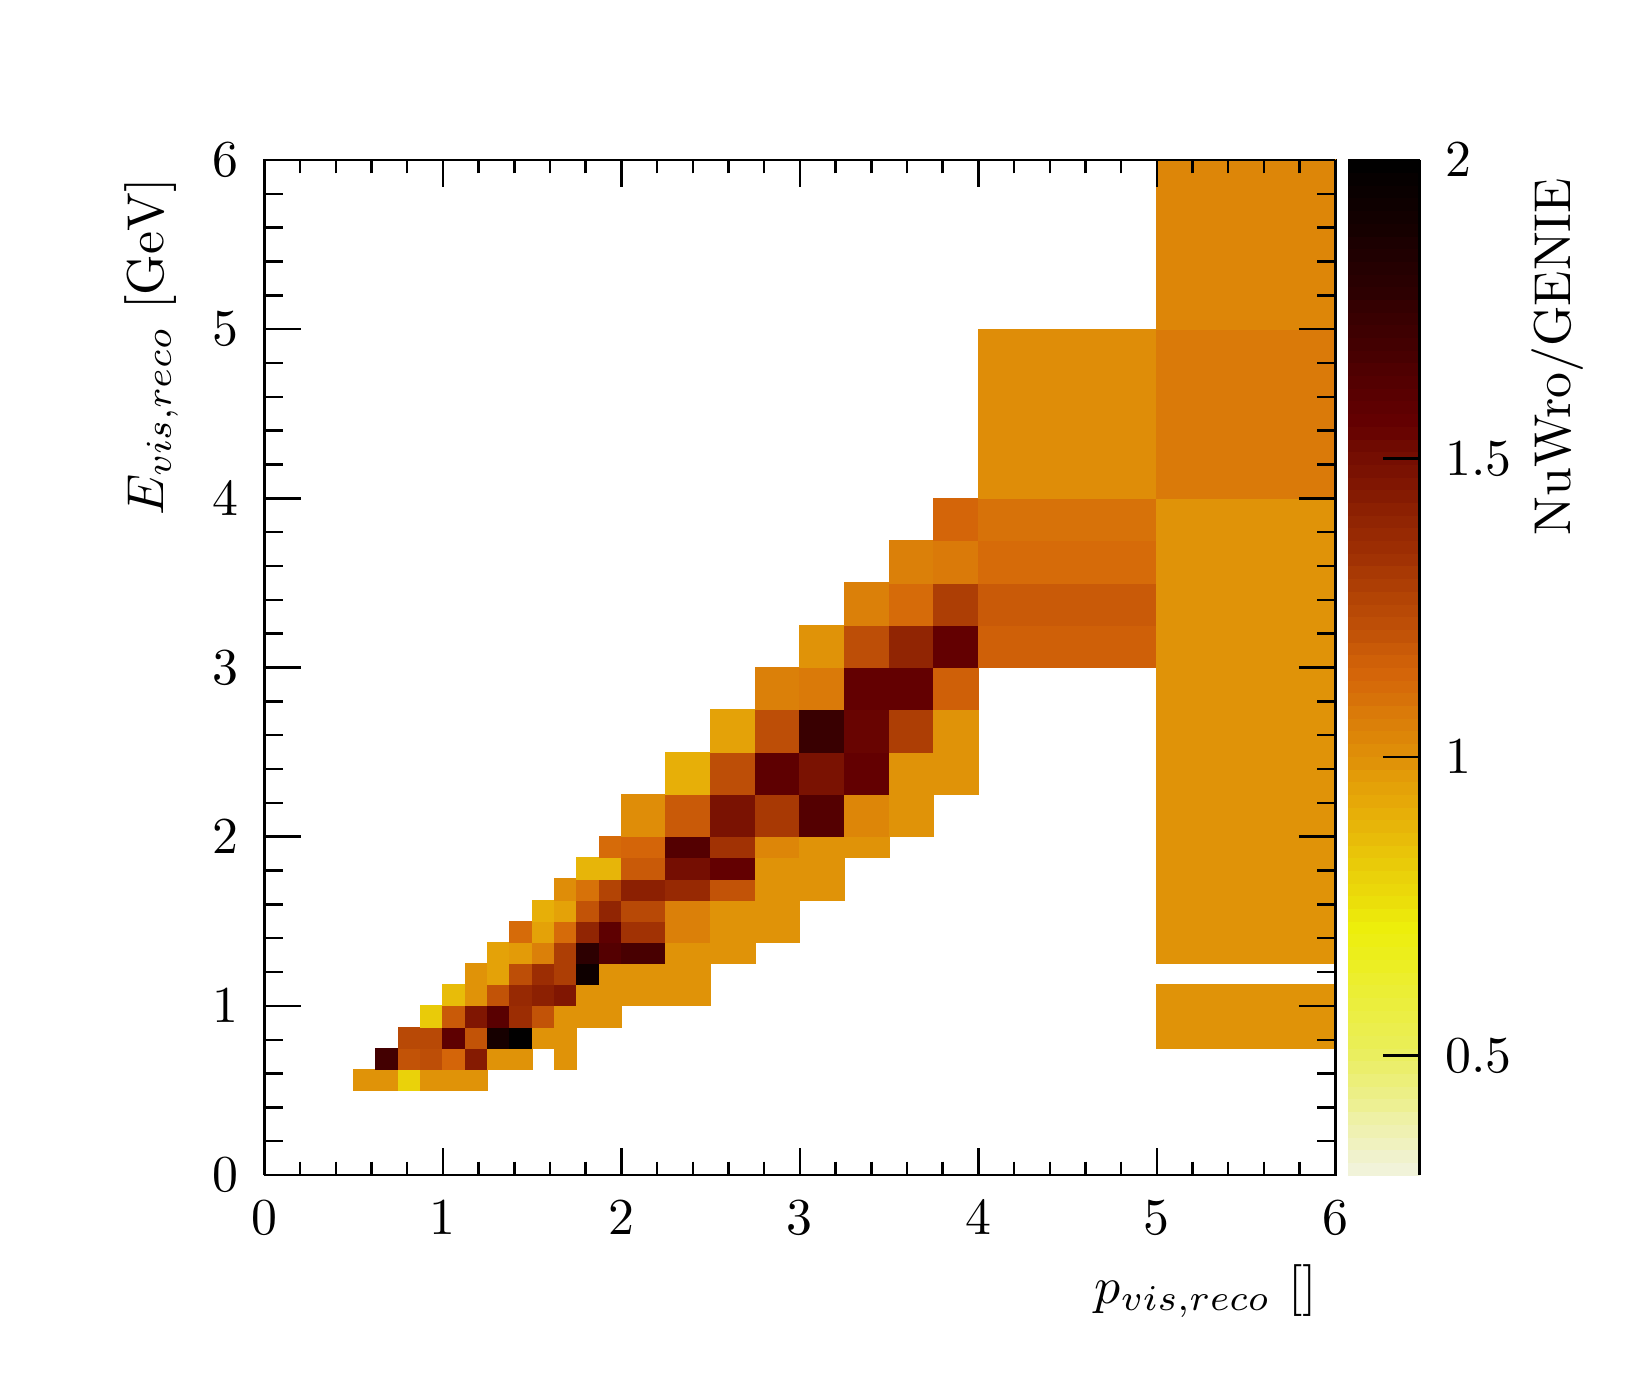
\begin{tikzpicture}
\pgfdeclareplotmark{cross} {
\pgfpathmoveto{\pgfpoint{-0.3\pgfplotmarksize}{\pgfplotmarksize}}
\pgfpathlineto{\pgfpoint{+0.3\pgfplotmarksize}{\pgfplotmarksize}}
\pgfpathlineto{\pgfpoint{+0.3\pgfplotmarksize}{0.3\pgfplotmarksize}}
\pgfpathlineto{\pgfpoint{+1\pgfplotmarksize}{0.3\pgfplotmarksize}}
\pgfpathlineto{\pgfpoint{+1\pgfplotmarksize}{-0.3\pgfplotmarksize}}
\pgfpathlineto{\pgfpoint{+0.3\pgfplotmarksize}{-0.3\pgfplotmarksize}}
\pgfpathlineto{\pgfpoint{+0.3\pgfplotmarksize}{-1.\pgfplotmarksize}}
\pgfpathlineto{\pgfpoint{-0.3\pgfplotmarksize}{-1.\pgfplotmarksize}}
\pgfpathlineto{\pgfpoint{-0.3\pgfplotmarksize}{-0.3\pgfplotmarksize}}
\pgfpathlineto{\pgfpoint{-1.\pgfplotmarksize}{-0.3\pgfplotmarksize}}
\pgfpathlineto{\pgfpoint{-1.\pgfplotmarksize}{0.3\pgfplotmarksize}}
\pgfpathlineto{\pgfpoint{-0.3\pgfplotmarksize}{0.3\pgfplotmarksize}}
\pgfpathclose
\pgfusepathqstroke
}
\pgfdeclareplotmark{cross*} {
\pgfpathmoveto{\pgfpoint{-0.3\pgfplotmarksize}{\pgfplotmarksize}}
\pgfpathlineto{\pgfpoint{+0.3\pgfplotmarksize}{\pgfplotmarksize}}
\pgfpathlineto{\pgfpoint{+0.3\pgfplotmarksize}{0.3\pgfplotmarksize}}
\pgfpathlineto{\pgfpoint{+1\pgfplotmarksize}{0.3\pgfplotmarksize}}
\pgfpathlineto{\pgfpoint{+1\pgfplotmarksize}{-0.3\pgfplotmarksize}}
\pgfpathlineto{\pgfpoint{+0.3\pgfplotmarksize}{-0.3\pgfplotmarksize}}
\pgfpathlineto{\pgfpoint{+0.3\pgfplotmarksize}{-1.\pgfplotmarksize}}
\pgfpathlineto{\pgfpoint{-0.3\pgfplotmarksize}{-1.\pgfplotmarksize}}
\pgfpathlineto{\pgfpoint{-0.3\pgfplotmarksize}{-0.3\pgfplotmarksize}}
\pgfpathlineto{\pgfpoint{-1.\pgfplotmarksize}{-0.3\pgfplotmarksize}}
\pgfpathlineto{\pgfpoint{-1.\pgfplotmarksize}{0.3\pgfplotmarksize}}
\pgfpathlineto{\pgfpoint{-0.3\pgfplotmarksize}{0.3\pgfplotmarksize}}
\pgfpathclose
\pgfusepathqfillstroke
}
\pgfdeclareplotmark{newstar} {
\pgfpathmoveto{\pgfqpoint{0pt}{\pgfplotmarksize}}
\pgfpathlineto{\pgfqpointpolar{44}{0.5\pgfplotmarksize}}
\pgfpathlineto{\pgfqpointpolar{18}{\pgfplotmarksize}}
\pgfpathlineto{\pgfqpointpolar{-20}{0.5\pgfplotmarksize}}
\pgfpathlineto{\pgfqpointpolar{-54}{\pgfplotmarksize}}
\pgfpathlineto{\pgfqpointpolar{-90}{0.5\pgfplotmarksize}}
\pgfpathlineto{\pgfqpointpolar{234}{\pgfplotmarksize}}
\pgfpathlineto{\pgfqpointpolar{198}{0.5\pgfplotmarksize}}
\pgfpathlineto{\pgfqpointpolar{162}{\pgfplotmarksize}}
\pgfpathlineto{\pgfqpointpolar{134}{0.5\pgfplotmarksize}}
\pgfpathclose
\pgfusepathqstroke
}
\pgfdeclareplotmark{newstar*} {
\pgfpathmoveto{\pgfqpoint{0pt}{\pgfplotmarksize}}
\pgfpathlineto{\pgfqpointpolar{44}{0.5\pgfplotmarksize}}
\pgfpathlineto{\pgfqpointpolar{18}{\pgfplotmarksize}}
\pgfpathlineto{\pgfqpointpolar{-20}{0.5\pgfplotmarksize}}
\pgfpathlineto{\pgfqpointpolar{-54}{\pgfplotmarksize}}
\pgfpathlineto{\pgfqpointpolar{-90}{0.5\pgfplotmarksize}}
\pgfpathlineto{\pgfqpointpolar{234}{\pgfplotmarksize}}
\pgfpathlineto{\pgfqpointpolar{198}{0.5\pgfplotmarksize}}
\pgfpathlineto{\pgfqpointpolar{162}{\pgfplotmarksize}}
\pgfpathlineto{\pgfqpointpolar{134}{0.5\pgfplotmarksize}}
\pgfpathclose
\pgfusepathqfillstroke
}
\definecolor{c}{rgb}{1,1,1};
\draw [color=c, fill=c] (0,0) rectangle (20,16.7416);
\draw [color=c, fill=c] (3,2.1764) rectangle (16.6,15.0674);
\definecolor{c}{rgb}{0,0,0};
\draw [c,line width=0.9] (3,2.1764) -- (3,15.0674) -- (16.6,15.0674) -- (16.6,2.1764) -- (3,2.1764);
\definecolor{c}{rgb}{1,1,1};
\draw [color=c, fill=c] (3,2.1764) rectangle (16.6,15.0674);
\definecolor{c}{rgb}{0,0,0};
\draw [c,line width=0.9] (3,2.1764) -- (3,15.0674) -- (16.6,15.0674) -- (16.6,2.1764) -- (3,2.1764);
\definecolor{c}{rgb}{0.879902,0.576716,0.032598};
\draw [color=c, fill=c] (4.13333,3.25066) rectangle (4.41667,3.51922);
\draw [color=c, fill=c] (4.41667,3.25066) rectangle (4.7,3.51922);
\definecolor{c}{rgb}{0.91826,0.821814,0.0383578};
\draw [color=c, fill=c] (4.7,3.25066) rectangle (4.98333,3.51922);
\definecolor{c}{rgb}{0.879902,0.576716,0.032598};
\draw [color=c, fill=c] (4.98333,3.25066) rectangle (5.26667,3.51922);
\draw [color=c, fill=c] (5.26667,3.25066) rectangle (5.55,3.51922);
\draw [color=c, fill=c] (5.55,3.25066) rectangle (5.83333,3.51922);
\definecolor{c}{rgb}{0.2625,0,0.00392157};
\draw [color=c, fill=c] (4.41667,3.51922) rectangle (4.7,3.78778);
\definecolor{c}{rgb}{0.762745,0.327451,0.0279412};
\draw [color=c, fill=c] (4.7,3.51922) rectangle (4.98333,3.78778);
\definecolor{c}{rgb}{0.742157,0.306863,0.0257353};
\draw [color=c, fill=c] (4.98333,3.51922) rectangle (5.26667,3.78778);
\definecolor{c}{rgb}{0.831373,0.396078,0.0352941};
\draw [color=c, fill=c] (5.26667,3.51922) rectangle (5.55,3.78778);
\definecolor{c}{rgb}{0.520956,0.104779,0.00857843};
\draw [color=c, fill=c] (5.55,3.51922) rectangle (5.83333,3.78778);
\definecolor{c}{rgb}{0.879902,0.576716,0.032598};
\draw [color=c, fill=c] (5.83333,3.51922) rectangle (6.11667,3.78778);
\draw [color=c, fill=c] (6.11667,3.51922) rectangle (6.4,3.78778);
\draw [color=c, fill=c] (6.68333,3.51922) rectangle (6.96667,3.78778);
\definecolor{c}{rgb}{0.721569,0.286275,0.0235294};
\draw [color=c, fill=c] (4.7,3.78778) rectangle (4.98333,4.05634);
\draw [color=c, fill=c] (4.98333,3.78778) rectangle (5.26667,4.05634);
\definecolor{c}{rgb}{0.368382,0,0.00392157};
\draw [color=c, fill=c] (5.26667,3.78778) rectangle (5.55,4.05634);
\definecolor{c}{rgb}{0.762745,0.327451,0.0279412};
\draw [color=c, fill=c] (5.55,3.78778) rectangle (5.83333,4.05634);
\definecolor{c}{rgb}{0.0882353,0,0.00196078};
\draw [color=c, fill=c] (5.83333,3.78778) rectangle (6.11667,4.05634);
\definecolor{c}{rgb}{0.00551471,0,0.000122549};
\draw [color=c, fill=c] (6.11667,3.78778) rectangle (6.4,4.05634);
\definecolor{c}{rgb}{0.879902,0.576716,0.032598};
\draw [color=c, fill=c] (6.4,3.78778) rectangle (6.68333,4.05634);
\draw [color=c, fill=c] (6.68333,3.78778) rectangle (6.96667,4.05634);
\draw [color=c, fill=c] (14.3333,3.78778) rectangle (16.6,4.05634);
\definecolor{c}{rgb}{0.915686,0.796078,0.0372549};
\draw [color=c, fill=c] (4.98333,4.05634) rectangle (5.26667,4.32491);
\definecolor{c}{rgb}{0.790196,0.354902,0.0308824};
\draw [color=c, fill=c] (5.26667,4.05634) rectangle (5.55,4.32491);
\definecolor{c}{rgb}{0.5,0.0882353,0.00784314};
\draw [color=c, fill=c] (5.55,4.05634) rectangle (5.83333,4.32491);
\definecolor{c}{rgb}{0.348529,0,0.00392157};
\draw [color=c, fill=c] (5.83333,4.05634) rectangle (6.11667,4.32491);
\definecolor{c}{rgb}{0.611765,0.176471,0.0117647};
\draw [color=c, fill=c] (6.11667,4.05634) rectangle (6.4,4.32491);
\definecolor{c}{rgb}{0.762745,0.327451,0.0279412};
\draw [color=c, fill=c] (6.4,4.05634) rectangle (6.68333,4.32491);
\definecolor{c}{rgb}{0.879902,0.576716,0.032598};
\draw [color=c, fill=c] (6.68333,4.05634) rectangle (6.96667,4.32491);
\draw [color=c, fill=c] (6.96667,4.05634) rectangle (7.25,4.32491);
\draw [color=c, fill=c] (7.25,4.05634) rectangle (7.53333,4.32491);
\draw [color=c, fill=c] (14.3333,4.05634) rectangle (16.6,4.32491);
\definecolor{c}{rgb}{0.909681,0.736029,0.0346814};
\draw [color=c, fill=c] (5.26667,4.32491) rectangle (5.55,4.59347);
\definecolor{c}{rgb}{0.879902,0.576716,0.032598};
\draw [color=c, fill=c] (5.55,4.32491) rectangle (5.83333,4.59347);
\definecolor{c}{rgb}{0.762745,0.327451,0.0279412};
\draw [color=c, fill=c] (5.83333,4.32491) rectangle (6.11667,4.59347);
\definecolor{c}{rgb}{0.590809,0.159926,0.0110294};
\draw [color=c, fill=c] (6.11667,4.32491) rectangle (6.4,4.59347);
\definecolor{c}{rgb}{0.548897,0.126838,0.00955882};
\draw [color=c, fill=c] (6.4,4.32491) rectangle (6.68333,4.59347);
\definecolor{c}{rgb}{0.5,0.0882353,0.00784314};
\draw [color=c, fill=c] (6.68333,4.32491) rectangle (6.96667,4.59347);
\definecolor{c}{rgb}{0.879902,0.576716,0.032598};
\draw [color=c, fill=c] (6.96667,4.32491) rectangle (7.25,4.59347);
\draw [color=c, fill=c] (7.25,4.32491) rectangle (7.53333,4.59347);
\draw [color=c, fill=c] (7.53333,4.32491) rectangle (8.1,4.59347);
\draw [color=c, fill=c] (8.1,4.32491) rectangle (8.66667,4.59347);
\draw [color=c, fill=c] (14.3333,4.32491) rectangle (16.6,4.59347);
\draw [color=c, fill=c] (5.55,4.59347) rectangle (5.83333,4.86203);
\definecolor{c}{rgb}{0.895343,0.634191,0.0317402};
\draw [color=c, fill=c] (5.83333,4.59347) rectangle (6.11667,4.86203);
\definecolor{c}{rgb}{0.742157,0.306863,0.0257353};
\draw [color=c, fill=c] (6.11667,4.59347) rectangle (6.4,4.86203);
\definecolor{c}{rgb}{0.611765,0.176471,0.0117647};
\draw [color=c, fill=c] (6.4,4.59347) rectangle (6.68333,4.86203);
\definecolor{c}{rgb}{0.680392,0.245098,0.0191176};
\draw [color=c, fill=c] (6.68333,4.59347) rectangle (6.96667,4.86203);
\definecolor{c}{rgb}{0.0551471,0,0.00122549};
\draw [color=c, fill=c] (6.96667,4.59347) rectangle (7.25,4.86203);
\definecolor{c}{rgb}{0.879902,0.576716,0.032598};
\draw [color=c, fill=c] (7.25,4.59347) rectangle (7.53333,4.86203);
\draw [color=c, fill=c] (7.53333,4.59347) rectangle (8.1,4.86203);
\draw [color=c, fill=c] (8.1,4.59347) rectangle (8.66667,4.86203);
\definecolor{c}{rgb}{0.895343,0.634191,0.0317402};
\draw [color=c, fill=c] (5.83333,4.86203) rectangle (6.11667,5.13059);
\definecolor{c}{rgb}{0.888726,0.609559,0.0321078};
\draw [color=c, fill=c] (6.11667,4.86203) rectangle (6.4,5.13059);
\definecolor{c}{rgb}{0.860049,0.502819,0.033701};
\draw [color=c, fill=c] (6.4,4.86203) rectangle (6.68333,5.13059);
\definecolor{c}{rgb}{0.680392,0.245098,0.0191176};
\draw [color=c, fill=c] (6.68333,4.86203) rectangle (6.96667,5.13059);
\definecolor{c}{rgb}{0.176471,0,0.00392157};
\draw [color=c, fill=c] (6.96667,4.86203) rectangle (7.25,5.13059);
\definecolor{c}{rgb}{0.328676,0,0.00392157};
\draw [color=c, fill=c] (7.25,4.86203) rectangle (7.53333,5.13059);
\definecolor{c}{rgb}{0.282353,0,0.00392157};
\draw [color=c, fill=c] (7.53333,4.86203) rectangle (8.1,5.13059);
\definecolor{c}{rgb}{0.879902,0.576716,0.032598};
\draw [color=c, fill=c] (8.1,4.86203) rectangle (8.66667,5.13059);
\draw [color=c, fill=c] (8.66667,4.86203) rectangle (9.23333,5.13059);
\draw [color=c, fill=c] (14.3333,4.86203) rectangle (16.6,5.13059);
\definecolor{c}{rgb}{0.83799,0.420711,0.0349265};
\draw [color=c, fill=c] (6.11667,5.13059) rectangle (6.4,5.39916);
\definecolor{c}{rgb}{0.895343,0.634191,0.0317402};
\draw [color=c, fill=c] (6.4,5.13059) rectangle (6.68333,5.39916);
\definecolor{c}{rgb}{0.83799,0.420711,0.0349265};
\draw [color=c, fill=c] (6.68333,5.13059) rectangle (6.96667,5.39916);
\definecolor{c}{rgb}{0.569853,0.143382,0.0102941};
\draw [color=c, fill=c] (6.96667,5.13059) rectangle (7.25,5.39916);
\definecolor{c}{rgb}{0.368382,0,0.00392157};
\draw [color=c, fill=c] (7.25,5.13059) rectangle (7.53333,5.39916);
\definecolor{c}{rgb}{0.632353,0.197059,0.0139706};
\draw [color=c, fill=c] (7.53333,5.13059) rectangle (8.1,5.39916);
\definecolor{c}{rgb}{0.860049,0.502819,0.033701};
\draw [color=c, fill=c] (8.1,5.13059) rectangle (8.66667,5.39916);
\definecolor{c}{rgb}{0.879902,0.576716,0.032598};
\draw [color=c, fill=c] (8.66667,5.13059) rectangle (9.23333,5.39916);
\draw [color=c, fill=c] (9.23333,5.13059) rectangle (9.8,5.39916);
\draw [color=c, fill=c] (14.3333,5.13059) rectangle (16.6,5.39916);
\definecolor{c}{rgb}{0.904534,0.684559,0.0324755};
\draw [color=c, fill=c] (6.4,5.39916) rectangle (6.68333,5.66772);
\definecolor{c}{rgb}{0.895343,0.634191,0.0317402};
\draw [color=c, fill=c] (6.68333,5.39916) rectangle (6.96667,5.66772);
\definecolor{c}{rgb}{0.762745,0.327451,0.0279412};
\draw [color=c, fill=c] (6.96667,5.39916) rectangle (7.25,5.66772);
\definecolor{c}{rgb}{0.569853,0.143382,0.0102941};
\draw [color=c, fill=c] (7.25,5.39916) rectangle (7.53333,5.66772);
\definecolor{c}{rgb}{0.721569,0.286275,0.0235294};
\draw [color=c, fill=c] (7.53333,5.39916) rectangle (8.1,5.66772);
\definecolor{c}{rgb}{0.860049,0.502819,0.033701};
\draw [color=c, fill=c] (8.1,5.39916) rectangle (8.66667,5.66772);
\definecolor{c}{rgb}{0.879902,0.576716,0.032598};
\draw [color=c, fill=c] (8.66667,5.39916) rectangle (9.23333,5.66772);
\draw [color=c, fill=c] (9.23333,5.39916) rectangle (9.8,5.66772);
\draw [color=c, fill=c] (14.3333,5.39916) rectangle (16.6,5.66772);
\definecolor{c}{rgb}{0.873284,0.552083,0.0329657};
\draw [color=c, fill=c] (6.68333,5.66772) rectangle (6.96667,5.93628);
\definecolor{c}{rgb}{0.844608,0.445343,0.0345588};
\draw [color=c, fill=c] (6.96667,5.66772) rectangle (7.25,5.93628);
\definecolor{c}{rgb}{0.70098,0.265686,0.0213235};
\draw [color=c, fill=c] (7.25,5.66772) rectangle (7.53333,5.93628);
\definecolor{c}{rgb}{0.548897,0.126838,0.00955882};
\draw [color=c, fill=c] (7.53333,5.66772) rectangle (8.1,5.93628);
\definecolor{c}{rgb}{0.590809,0.159926,0.0110294};
\draw [color=c, fill=c] (8.1,5.66772) rectangle (8.66667,5.93628);
\definecolor{c}{rgb}{0.762745,0.327451,0.0279412};
\draw [color=c, fill=c] (8.66667,5.66772) rectangle (9.23333,5.93628);
\definecolor{c}{rgb}{0.879902,0.576716,0.032598};
\draw [color=c, fill=c] (9.23333,5.66772) rectangle (9.8,5.93628);
\draw [color=c, fill=c] (9.8,5.66772) rectangle (10.3667,5.93628);
\draw [color=c, fill=c] (14.3333,5.66772) rectangle (16.6,5.93628);
\definecolor{c}{rgb}{0.907108,0.710294,0.0335784};
\draw [color=c, fill=c] (6.96667,5.93628) rectangle (7.25,6.20485);
\draw [color=c, fill=c] (7.25,5.93628) rectangle (7.53333,6.20485);
\definecolor{c}{rgb}{0.790196,0.354902,0.0308824};
\draw [color=c, fill=c] (7.53333,5.93628) rectangle (8.1,6.20485);
\definecolor{c}{rgb}{0.458088,0.0551471,0.00637255};
\draw [color=c, fill=c] (8.1,5.93628) rectangle (8.66667,6.20485);
\definecolor{c}{rgb}{0.388235,0,0.00392157};
\draw [color=c, fill=c] (8.66667,5.93628) rectangle (9.23333,6.20485);
\definecolor{c}{rgb}{0.879902,0.576716,0.032598};
\draw [color=c, fill=c] (9.23333,5.93628) rectangle (9.8,6.20485);
\draw [color=c, fill=c] (9.8,5.93628) rectangle (10.3667,6.20485);
\draw [color=c, fill=c] (14.3333,5.93628) rectangle (16.6,6.20485);
\definecolor{c}{rgb}{0.83799,0.420711,0.0349265};
\draw [color=c, fill=c] (7.25,6.20485) rectangle (7.53333,6.47341);
\definecolor{c}{rgb}{0.831373,0.396078,0.0352941};
\draw [color=c, fill=c] (7.53333,6.20485) rectangle (8.1,6.47341);
\definecolor{c}{rgb}{0.328676,0,0.00392157};
\draw [color=c, fill=c] (8.1,6.20485) rectangle (8.66667,6.47341);
\definecolor{c}{rgb}{0.632353,0.197059,0.0139706};
\draw [color=c, fill=c] (8.66667,6.20485) rectangle (9.23333,6.47341);
\definecolor{c}{rgb}{0.866667,0.527451,0.0333333};
\draw [color=c, fill=c] (9.23333,6.20485) rectangle (9.8,6.47341);
\definecolor{c}{rgb}{0.879902,0.576716,0.032598};
\draw [color=c, fill=c] (9.8,6.20485) rectangle (10.3667,6.47341);
\draw [color=c, fill=c] (10.3667,6.20485) rectangle (10.9333,6.47341);
\draw [color=c, fill=c] (14.3333,6.20485) rectangle (16.6,6.47341);
\definecolor{c}{rgb}{0.873284,0.552083,0.0329657};
\draw [color=c, fill=c] (7.53333,6.47341) rectangle (8.1,7.01053);
\definecolor{c}{rgb}{0.790196,0.354902,0.0308824};
\draw [color=c, fill=c] (8.1,6.47341) rectangle (8.66667,7.01053);
\definecolor{c}{rgb}{0.479044,0.0716912,0.00710784};
\draw [color=c, fill=c] (8.66667,6.47341) rectangle (9.23333,7.01053);
\definecolor{c}{rgb}{0.659804,0.22451,0.0169118};
\draw [color=c, fill=c] (9.23333,6.47341) rectangle (9.8,7.01053);
\definecolor{c}{rgb}{0.328676,0,0.00392157};
\draw [color=c, fill=c] (9.8,6.47341) rectangle (10.3667,7.01053);
\definecolor{c}{rgb}{0.866667,0.527451,0.0333333};
\draw [color=c, fill=c] (10.3667,6.47341) rectangle (10.9333,7.01053);
\definecolor{c}{rgb}{0.879902,0.576716,0.032598};
\draw [color=c, fill=c] (10.9333,6.47341) rectangle (11.5,7.01053);
\draw [color=c, fill=c] (14.3333,6.47341) rectangle (16.6,7.01053);
\definecolor{c}{rgb}{0.904534,0.684559,0.0324755};
\draw [color=c, fill=c] (8.1,7.01053) rectangle (8.66667,7.54766);
\definecolor{c}{rgb}{0.742157,0.306863,0.0257353};
\draw [color=c, fill=c] (8.66667,7.01053) rectangle (9.23333,7.54766);
\definecolor{c}{rgb}{0.368382,0,0.00392157};
\draw [color=c, fill=c] (9.23333,7.01053) rectangle (9.8,7.54766);
\definecolor{c}{rgb}{0.479044,0.0716912,0.00710784};
\draw [color=c, fill=c] (9.8,7.01053) rectangle (10.3667,7.54766);
\definecolor{c}{rgb}{0.388235,0,0.00392157};
\draw [color=c, fill=c] (10.3667,7.01053) rectangle (10.9333,7.54766);
\definecolor{c}{rgb}{0.879902,0.576716,0.032598};
\draw [color=c, fill=c] (10.9333,7.01053) rectangle (11.5,7.54766);
\draw [color=c, fill=c] (11.5,7.01053) rectangle (12.0667,7.54766);
\draw [color=c, fill=c] (14.3333,7.01053) rectangle (16.6,7.54766);
\definecolor{c}{rgb}{0.895343,0.634191,0.0317402};
\draw [color=c, fill=c] (8.66667,7.54766) rectangle (9.23333,8.08478);
\definecolor{c}{rgb}{0.742157,0.306863,0.0257353};
\draw [color=c, fill=c] (9.23333,7.54766) rectangle (9.8,8.08478);
\definecolor{c}{rgb}{0.222794,0,0.00392157};
\draw [color=c, fill=c] (9.8,7.54766) rectangle (10.3667,8.08478);
\definecolor{c}{rgb}{0.409191,0.0165441,0.00465686};
\draw [color=c, fill=c] (10.3667,7.54766) rectangle (10.9333,8.08478);
\definecolor{c}{rgb}{0.680392,0.245098,0.0191176};
\draw [color=c, fill=c] (10.9333,7.54766) rectangle (11.5,8.08478);
\definecolor{c}{rgb}{0.879902,0.576716,0.032598};
\draw [color=c, fill=c] (11.5,7.54766) rectangle (12.0667,8.08478);
\draw [color=c, fill=c] (14.3333,7.54766) rectangle (16.6,8.08478);
\definecolor{c}{rgb}{0.860049,0.502819,0.033701};
\draw [color=c, fill=c] (9.23333,8.08478) rectangle (9.8,8.62191);
\definecolor{c}{rgb}{0.853431,0.478186,0.0340686};
\draw [color=c, fill=c] (9.8,8.08478) rectangle (10.3667,8.62191);
\definecolor{c}{rgb}{0.388235,0,0.00392157};
\draw [color=c, fill=c] (10.3667,8.08478) rectangle (10.9333,8.62191);
\draw [color=c, fill=c] (10.9333,8.08478) rectangle (11.5,8.62191);
\definecolor{c}{rgb}{0.810784,0.37549,0.0330882};
\draw [color=c, fill=c] (11.5,8.08478) rectangle (12.0667,8.62191);
\definecolor{c}{rgb}{0.879902,0.576716,0.032598};
\draw [color=c, fill=c] (14.3333,8.08478) rectangle (16.6,8.62191);
\draw [color=c, fill=c] (9.8,8.62191) rectangle (10.3667,9.15904);
\definecolor{c}{rgb}{0.742157,0.306863,0.0257353};
\draw [color=c, fill=c] (10.3667,8.62191) rectangle (10.9333,9.15904);
\definecolor{c}{rgb}{0.569853,0.143382,0.0102941};
\draw [color=c, fill=c] (10.9333,8.62191) rectangle (11.5,9.15904);
\definecolor{c}{rgb}{0.388235,0,0.00392157};
\draw [color=c, fill=c] (11.5,8.62191) rectangle (12.0667,9.15904);
\definecolor{c}{rgb}{0.810784,0.37549,0.0330882};
\draw [color=c, fill=c] (12.0667,8.62191) rectangle (14.3333,9.15904);
\definecolor{c}{rgb}{0.879902,0.576716,0.032598};
\draw [color=c, fill=c] (14.3333,8.62191) rectangle (16.6,9.15904);
\definecolor{c}{rgb}{0.860049,0.502819,0.033701};
\draw [color=c, fill=c] (10.3667,9.15904) rectangle (10.9333,9.69616);
\definecolor{c}{rgb}{0.83799,0.420711,0.0349265};
\draw [color=c, fill=c] (10.9333,9.15904) rectangle (11.5,9.69616);
\definecolor{c}{rgb}{0.680392,0.245098,0.0191176};
\draw [color=c, fill=c] (11.5,9.15904) rectangle (12.0667,9.69616);
\definecolor{c}{rgb}{0.790196,0.354902,0.0308824};
\draw [color=c, fill=c] (12.0667,9.15904) rectangle (14.3333,9.69616);
\definecolor{c}{rgb}{0.879902,0.576716,0.032598};
\draw [color=c, fill=c] (14.3333,9.15904) rectangle (16.6,9.69616);
\definecolor{c}{rgb}{0.860049,0.502819,0.033701};
\draw [color=c, fill=c] (10.9333,9.69616) rectangle (11.5,10.2333);
\definecolor{c}{rgb}{0.853431,0.478186,0.0340686};
\draw [color=c, fill=c] (11.5,9.69616) rectangle (12.0667,10.2333);
\definecolor{c}{rgb}{0.83799,0.420711,0.0349265};
\draw [color=c, fill=c] (12.0667,9.69616) rectangle (14.3333,10.2333);
\definecolor{c}{rgb}{0.879902,0.576716,0.032598};
\draw [color=c, fill=c] (14.3333,9.69616) rectangle (16.6,10.2333);
\definecolor{c}{rgb}{0.831373,0.396078,0.0352941};
\draw [color=c, fill=c] (11.5,10.2333) rectangle (12.0667,10.7704);
\definecolor{c}{rgb}{0.844608,0.445343,0.0345588};
\draw [color=c, fill=c] (12.0667,10.2333) rectangle (14.3333,10.7704);
\definecolor{c}{rgb}{0.879902,0.576716,0.032598};
\draw [color=c, fill=c] (14.3333,10.2333) rectangle (16.6,10.7704);
\definecolor{c}{rgb}{0.873284,0.552083,0.0329657};
\draw [color=c, fill=c] (12.0667,10.7704) rectangle (14.3333,12.9189);
\definecolor{c}{rgb}{0.853431,0.478186,0.0340686};
\draw [color=c, fill=c] (14.3333,10.7704) rectangle (16.6,12.9189);
\definecolor{c}{rgb}{0.866667,0.527451,0.0333333};
\draw [color=c, fill=c] (14.3333,12.9189) rectangle (16.6,15.0674);
\definecolor{c}{rgb}{0,0,0};
\draw [c,line width=0.9] (3,2.1764) -- (16.6,2.1764);
\draw [c,line width=0.9] (3,2.51793) -- (3,2.1764);
\draw [c,line width=0.9] (3.45333,2.34717) -- (3.45333,2.1764);
\draw [c,line width=0.9] (3.90667,2.34717) -- (3.90667,2.1764);
\draw [c,line width=0.9] (4.36,2.34717) -- (4.36,2.1764);
\draw [c,line width=0.9] (4.81333,2.34717) -- (4.81333,2.1764);
\draw [c,line width=0.9] (5.26667,2.51793) -- (5.26667,2.1764);
\draw [c,line width=0.9] (5.72,2.34717) -- (5.72,2.1764);
\draw [c,line width=0.9] (6.17333,2.34717) -- (6.17333,2.1764);
\draw [c,line width=0.9] (6.62667,2.34717) -- (6.62667,2.1764);
\draw [c,line width=0.9] (7.08,2.34717) -- (7.08,2.1764);
\draw [c,line width=0.9] (7.53333,2.51793) -- (7.53333,2.1764);
\draw [c,line width=0.9] (7.98667,2.34717) -- (7.98667,2.1764);
\draw [c,line width=0.9] (8.44,2.34717) -- (8.44,2.1764);
\draw [c,line width=0.9] (8.89333,2.34717) -- (8.89333,2.1764);
\draw [c,line width=0.9] (9.34667,2.34717) -- (9.34667,2.1764);
\draw [c,line width=0.9] (9.8,2.51793) -- (9.8,2.1764);
\draw [c,line width=0.9] (10.2533,2.34717) -- (10.2533,2.1764);
\draw [c,line width=0.9] (10.7067,2.34717) -- (10.7067,2.1764);
\draw [c,line width=0.9] (11.16,2.34717) -- (11.16,2.1764);
\draw [c,line width=0.9] (11.6133,2.34717) -- (11.6133,2.1764);
\draw [c,line width=0.9] (12.0667,2.51793) -- (12.0667,2.1764);
\draw [c,line width=0.9] (12.52,2.34717) -- (12.52,2.1764);
\draw [c,line width=0.9] (12.9733,2.34717) -- (12.9733,2.1764);
\draw [c,line width=0.9] (13.4267,2.34717) -- (13.4267,2.1764);
\draw [c,line width=0.9] (13.88,2.34717) -- (13.88,2.1764);
\draw [c,line width=0.9] (14.3333,2.51793) -- (14.3333,2.1764);
\draw [c,line width=0.9] (14.7867,2.34717) -- (14.7867,2.1764);
\draw [c,line width=0.9] (15.24,2.34717) -- (15.24,2.1764);
\draw [c,line width=0.9] (15.6933,2.34717) -- (15.6933,2.1764);
\draw [c,line width=0.9] (16.1467,2.34717) -- (16.1467,2.1764);
\draw [c,line width=0.9] (16.6,2.51793) -- (16.6,2.1764);
\draw [anchor=base] (3,1.42303) node[scale=1.8716, color=c, rotate=0]{0};
\draw [anchor=base] (5.26667,1.42303) node[scale=1.8716, color=c, rotate=0]{1};
\draw [anchor=base] (7.53333,1.42303) node[scale=1.8716, color=c, rotate=0]{2};
\draw [anchor=base] (9.8,1.42303) node[scale=1.8716, color=c, rotate=0]{3};
\draw [anchor=base] (12.0667,1.42303) node[scale=1.8716, color=c, rotate=0]{4};
\draw [anchor=base] (14.3333,1.42303) node[scale=1.8716, color=c, rotate=0]{5};
\draw [anchor=base] (16.6,1.42303) node[scale=1.8716, color=c, rotate=0]{6};
\draw [anchor= east] (16.6,0.703146) node[scale=1.8716, color=c, rotate=0]{$ p_{\text{vis, reco}}$ [\si{\GeV\per\clight}] };
\draw [c,line width=0.9] (3,15.0674) -- (16.6,15.0674);
\draw [c,line width=0.9] (3,14.7259) -- (3,15.0674);
\draw [c,line width=0.9] (3.45333,14.8967) -- (3.45333,15.0674);
\draw [c,line width=0.9] (3.90667,14.8967) -- (3.90667,15.0674);
\draw [c,line width=0.9] (4.36,14.8967) -- (4.36,15.0674);
\draw [c,line width=0.9] (4.81333,14.8967) -- (4.81333,15.0674);
\draw [c,line width=0.9] (5.26667,14.7259) -- (5.26667,15.0674);
\draw [c,line width=0.9] (5.72,14.8967) -- (5.72,15.0674);
\draw [c,line width=0.9] (6.17333,14.8967) -- (6.17333,15.0674);
\draw [c,line width=0.9] (6.62667,14.8967) -- (6.62667,15.0674);
\draw [c,line width=0.9] (7.08,14.8967) -- (7.08,15.0674);
\draw [c,line width=0.9] (7.53333,14.7259) -- (7.53333,15.0674);
\draw [c,line width=0.9] (7.98667,14.8967) -- (7.98667,15.0674);
\draw [c,line width=0.9] (8.44,14.8967) -- (8.44,15.0674);
\draw [c,line width=0.9] (8.89333,14.8967) -- (8.89333,15.0674);
\draw [c,line width=0.9] (9.34667,14.8967) -- (9.34667,15.0674);
\draw [c,line width=0.9] (9.8,14.7259) -- (9.8,15.0674);
\draw [c,line width=0.9] (10.2533,14.8967) -- (10.2533,15.0674);
\draw [c,line width=0.9] (10.7067,14.8967) -- (10.7067,15.0674);
\draw [c,line width=0.9] (11.16,14.8967) -- (11.16,15.0674);
\draw [c,line width=0.9] (11.6133,14.8967) -- (11.6133,15.0674);
\draw [c,line width=0.9] (12.0667,14.7259) -- (12.0667,15.0674);
\draw [c,line width=0.9] (12.52,14.8967) -- (12.52,15.0674);
\draw [c,line width=0.9] (12.9733,14.8967) -- (12.9733,15.0674);
\draw [c,line width=0.9] (13.4267,14.8967) -- (13.4267,15.0674);
\draw [c,line width=0.9] (13.88,14.8967) -- (13.88,15.0674);
\draw [c,line width=0.9] (14.3333,14.7259) -- (14.3333,15.0674);
\draw [c,line width=0.9] (14.7867,14.8967) -- (14.7867,15.0674);
\draw [c,line width=0.9] (15.24,14.8967) -- (15.24,15.0674);
\draw [c,line width=0.9] (15.6933,14.8967) -- (15.6933,15.0674);
\draw [c,line width=0.9] (16.1467,14.8967) -- (16.1467,15.0674);
\draw [c,line width=0.9] (16.6,14.7259) -- (16.6,15.0674);
\draw [c,line width=0.9] (3,2.1764) -- (3,15.0674);
\draw [c,line width=0.9] (3.462,2.1764) -- (3,2.1764);
\draw [c,line width=0.9] (3.231,2.6061) -- (3,2.6061);
\draw [c,line width=0.9] (3.231,3.03581) -- (3,3.03581);
\draw [c,line width=0.9] (3.231,3.46551) -- (3,3.46551);
\draw [c,line width=0.9] (3.231,3.89521) -- (3,3.89521);
\draw [c,line width=0.9] (3.462,4.32491) -- (3,4.32491);
\draw [c,line width=0.9] (3.231,4.75461) -- (3,4.75461);
\draw [c,line width=0.9] (3.231,5.18431) -- (3,5.18431);
\draw [c,line width=0.9] (3.231,5.61401) -- (3,5.61401);
\draw [c,line width=0.9] (3.231,6.04371) -- (3,6.04371);
\draw [c,line width=0.9] (3.462,6.47341) -- (3,6.47341);
\draw [c,line width=0.9] (3.231,6.90311) -- (3,6.90311);
\draw [c,line width=0.9] (3.231,7.33281) -- (3,7.33281);
\draw [c,line width=0.9] (3.231,7.76251) -- (3,7.76251);
\draw [c,line width=0.9] (3.231,8.19221) -- (3,8.19221);
\draw [c,line width=0.9] (3.462,8.62191) -- (3,8.62191);
\draw [c,line width=0.9] (3.231,9.05161) -- (3,9.05161);
\draw [c,line width=0.9] (3.231,9.48131) -- (3,9.48131);
\draw [c,line width=0.9] (3.231,9.91101) -- (3,9.91101);
\draw [c,line width=0.9] (3.231,10.3407) -- (3,10.3407);
\draw [c,line width=0.9] (3.462,10.7704) -- (3,10.7704);
\draw [c,line width=0.9] (3.231,11.2001) -- (3,11.2001);
\draw [c,line width=0.9] (3.231,11.6298) -- (3,11.6298);
\draw [c,line width=0.9] (3.231,12.0595) -- (3,12.0595);
\draw [c,line width=0.9] (3.231,12.4892) -- (3,12.4892);
\draw [c,line width=0.9] (3.462,12.9189) -- (3,12.9189);
\draw [c,line width=0.9] (3.231,13.3486) -- (3,13.3486);
\draw [c,line width=0.9] (3.231,13.7783) -- (3,13.7783);
\draw [c,line width=0.9] (3.231,14.208) -- (3,14.208);
\draw [c,line width=0.9] (3.231,14.6377) -- (3,14.6377);
\draw [c,line width=0.9] (3.462,15.0674) -- (3,15.0674);
\draw [anchor= east] (2.9,2.1764) node[scale=1.8716, color=c, rotate=0]{0};
\draw [anchor= east] (2.9,4.32491) node[scale=1.8716, color=c, rotate=0]{1};
\draw [anchor= east] (2.9,6.47341) node[scale=1.8716, color=c, rotate=0]{2};
\draw [anchor= east] (2.9,8.62191) node[scale=1.8716, color=c, rotate=0]{3};
\draw [anchor= east] (2.9,10.7704) node[scale=1.8716, color=c, rotate=0]{4};
\draw [anchor= east] (2.9,12.9189) node[scale=1.8716, color=c, rotate=0]{5};
\draw [anchor= east] (2.9,15.0674) node[scale=1.8716, color=c, rotate=0]{6};
\draw [anchor= east] (1.56,15.0674) node[scale=1.8716, color=c, rotate=90]{$E_{\text{vis, reco}}$ [\si{GeV}] };
\draw [c,line width=0.9] (16.6,2.1764) -- (16.6,15.0674);
\draw [c,line width=0.9] (16.138,2.1764) -- (16.6,2.1764);
\draw [c,line width=0.9] (16.369,2.6061) -- (16.6,2.6061);
\draw [c,line width=0.9] (16.369,3.03581) -- (16.6,3.03581);
\draw [c,line width=0.9] (16.369,3.46551) -- (16.6,3.46551);
\draw [c,line width=0.9] (16.369,3.89521) -- (16.6,3.89521);
\draw [c,line width=0.9] (16.138,4.32491) -- (16.6,4.32491);
\draw [c,line width=0.9] (16.369,4.75461) -- (16.6,4.75461);
\draw [c,line width=0.9] (16.369,5.18431) -- (16.6,5.18431);
\draw [c,line width=0.9] (16.369,5.61401) -- (16.6,5.61401);
\draw [c,line width=0.9] (16.369,6.04371) -- (16.6,6.04371);
\draw [c,line width=0.9] (16.138,6.47341) -- (16.6,6.47341);
\draw [c,line width=0.9] (16.369,6.90311) -- (16.6,6.90311);
\draw [c,line width=0.9] (16.369,7.33281) -- (16.6,7.33281);
\draw [c,line width=0.9] (16.369,7.76251) -- (16.6,7.76251);
\draw [c,line width=0.9] (16.369,8.19221) -- (16.6,8.19221);
\draw [c,line width=0.9] (16.138,8.62191) -- (16.6,8.62191);
\draw [c,line width=0.9] (16.369,9.05161) -- (16.6,9.05161);
\draw [c,line width=0.9] (16.369,9.48131) -- (16.6,9.48131);
\draw [c,line width=0.9] (16.369,9.91101) -- (16.6,9.91101);
\draw [c,line width=0.9] (16.369,10.3407) -- (16.6,10.3407);
\draw [c,line width=0.9] (16.138,10.7704) -- (16.6,10.7704);
\draw [c,line width=0.9] (16.369,11.2001) -- (16.6,11.2001);
\draw [c,line width=0.9] (16.369,11.6298) -- (16.6,11.6298);
\draw [c,line width=0.9] (16.369,12.0595) -- (16.6,12.0595);
\draw [c,line width=0.9] (16.369,12.4892) -- (16.6,12.4892);
\draw [c,line width=0.9] (16.138,12.9189) -- (16.6,12.9189);
\draw [c,line width=0.9] (16.369,13.3486) -- (16.6,13.3486);
\draw [c,line width=0.9] (16.369,13.7783) -- (16.6,13.7783);
\draw [c,line width=0.9] (16.369,14.208) -- (16.6,14.208);
\draw [c,line width=0.9] (16.369,14.6377) -- (16.6,14.6377);
\draw [c,line width=0.9] (16.138,15.0674) -- (16.6,15.0674);
\definecolor{c}{rgb}{0.945984,0.951044,0.850727};
\draw [color=c, fill=c] (16.7697,2.17697) rectangle (17.6685,2.33813);
\definecolor{c}{rgb}{0.942948,0.949146,0.799494};
\draw [color=c, fill=c] (16.7697,2.33813) rectangle (17.6685,2.4993);
\definecolor{c}{rgb}{0.939911,0.947249,0.748261};
\draw [color=c, fill=c] (16.7697,2.4993) rectangle (17.6685,2.66046);
\definecolor{c}{rgb}{0.936875,0.945351,0.697027};
\draw [color=c, fill=c] (16.7697,2.66046) rectangle (17.6685,2.82163);
\definecolor{c}{rgb}{0.933839,0.943453,0.645794};
\draw [color=c, fill=c] (16.7697,2.82163) rectangle (17.6685,2.9828);
\definecolor{c}{rgb}{0.929791,0.940923,0.577483};
\draw [color=c, fill=c] (16.7697,2.9828) rectangle (17.6685,3.14396);
\definecolor{c}{rgb}{0.926755,0.939026,0.526249};
\draw [color=c, fill=c] (16.7697,3.14396) rectangle (17.6685,3.30513);
\definecolor{c}{rgb}{0.923719,0.937128,0.475016};
\draw [color=c, fill=c] (16.7697,3.30513) rectangle (17.6685,3.46629);
\definecolor{c}{rgb}{0.920683,0.935231,0.423782};
\draw [color=c, fill=c] (16.7697,3.46629) rectangle (17.6685,3.62746);
\definecolor{c}{rgb}{0.917647,0.933333,0.372549};
\draw [color=c, fill=c] (16.7697,3.62746) rectangle (17.6685,3.78862);
\definecolor{c}{rgb}{0.919118,0.933333,0.331373};
\draw [color=c, fill=c] (16.7697,3.78862) rectangle (17.6685,3.94979);
\definecolor{c}{rgb}{0.920221,0.933333,0.30049};
\draw [color=c, fill=c] (16.7697,3.94979) rectangle (17.6685,4.11096);
\definecolor{c}{rgb}{0.921324,0.933333,0.269608};
\draw [color=c, fill=c] (16.7697,4.11096) rectangle (17.6685,4.27212);
\definecolor{c}{rgb}{0.922426,0.933333,0.238725};
\draw [color=c, fill=c] (16.7697,4.27212) rectangle (17.6685,4.43329);
\definecolor{c}{rgb}{0.923529,0.933333,0.207843};
\draw [color=c, fill=c] (16.7697,4.43329) rectangle (17.6685,4.59445);
\definecolor{c}{rgb}{0.924632,0.933333,0.176961};
\draw [color=c, fill=c] (16.7697,4.59445) rectangle (17.6685,4.75562);
\definecolor{c}{rgb}{0.926103,0.933333,0.135784};
\draw [color=c, fill=c] (16.7697,4.75562) rectangle (17.6685,4.91678);
\definecolor{c}{rgb}{0.927206,0.933333,0.104902};
\draw [color=c, fill=c] (16.7697,4.91678) rectangle (17.6685,5.07795);
\definecolor{c}{rgb}{0.928309,0.933333,0.0740196};
\draw [color=c, fill=c] (16.7697,5.07795) rectangle (17.6685,5.23912);
\definecolor{c}{rgb}{0.929412,0.933333,0.0431373};
\draw [color=c, fill=c] (16.7697,5.23912) rectangle (17.6685,5.40028);
\definecolor{c}{rgb}{0.926838,0.907598,0.0420343};
\draw [color=c, fill=c] (16.7697,5.40028) rectangle (17.6685,5.56145);
\definecolor{c}{rgb}{0.923407,0.873284,0.0405637};
\draw [color=c, fill=c] (16.7697,5.56145) rectangle (17.6685,5.72261);
\definecolor{c}{rgb}{0.920833,0.847549,0.0394608};
\draw [color=c, fill=c] (16.7697,5.72261) rectangle (17.6685,5.88378);
\definecolor{c}{rgb}{0.91826,0.821814,0.0383578};
\draw [color=c, fill=c] (16.7697,5.88378) rectangle (17.6685,6.04494);
\definecolor{c}{rgb}{0.915686,0.796078,0.0372549};
\draw [color=c, fill=c] (16.7697,6.04494) rectangle (17.6685,6.20611);
\definecolor{c}{rgb}{0.913113,0.770343,0.036152};
\draw [color=c, fill=c] (16.7697,6.20611) rectangle (17.6685,6.36728);
\definecolor{c}{rgb}{0.909681,0.736029,0.0346814};
\draw [color=c, fill=c] (16.7697,6.36728) rectangle (17.6685,6.52844);
\definecolor{c}{rgb}{0.907108,0.710294,0.0335784};
\draw [color=c, fill=c] (16.7697,6.52844) rectangle (17.6685,6.68961);
\definecolor{c}{rgb}{0.904534,0.684559,0.0324755};
\draw [color=c, fill=c] (16.7697,6.68961) rectangle (17.6685,6.85077);
\definecolor{c}{rgb}{0.901961,0.658824,0.0313726};
\draw [color=c, fill=c] (16.7697,6.85077) rectangle (17.6685,7.01194);
\definecolor{c}{rgb}{0.895343,0.634191,0.0317402};
\draw [color=c, fill=c] (16.7697,7.01194) rectangle (17.6685,7.1731);
\definecolor{c}{rgb}{0.888726,0.609559,0.0321078};
\draw [color=c, fill=c] (16.7697,7.1731) rectangle (17.6685,7.33427);
\definecolor{c}{rgb}{0.879902,0.576716,0.032598};
\draw [color=c, fill=c] (16.7697,7.33427) rectangle (17.6685,7.49544);
\definecolor{c}{rgb}{0.873284,0.552083,0.0329657};
\draw [color=c, fill=c] (16.7697,7.49544) rectangle (17.6685,7.6566);
\definecolor{c}{rgb}{0.866667,0.527451,0.0333333};
\draw [color=c, fill=c] (16.7697,7.6566) rectangle (17.6685,7.81777);
\definecolor{c}{rgb}{0.860049,0.502819,0.033701};
\draw [color=c, fill=c] (16.7697,7.81777) rectangle (17.6685,7.97893);
\definecolor{c}{rgb}{0.853431,0.478186,0.0340686};
\draw [color=c, fill=c] (16.7697,7.97893) rectangle (17.6685,8.1401);
\definecolor{c}{rgb}{0.844608,0.445343,0.0345588};
\draw [color=c, fill=c] (16.7697,8.1401) rectangle (17.6685,8.30126);
\definecolor{c}{rgb}{0.83799,0.420711,0.0349265};
\draw [color=c, fill=c] (16.7697,8.30126) rectangle (17.6685,8.46243);
\definecolor{c}{rgb}{0.831373,0.396078,0.0352941};
\draw [color=c, fill=c] (16.7697,8.46243) rectangle (17.6685,8.6236);
\definecolor{c}{rgb}{0.810784,0.37549,0.0330882};
\draw [color=c, fill=c] (16.7697,8.6236) rectangle (17.6685,8.78476);
\definecolor{c}{rgb}{0.790196,0.354902,0.0308824};
\draw [color=c, fill=c] (16.7697,8.78476) rectangle (17.6685,8.94593);
\definecolor{c}{rgb}{0.762745,0.327451,0.0279412};
\draw [color=c, fill=c] (16.7697,8.94593) rectangle (17.6685,9.10709);
\definecolor{c}{rgb}{0.742157,0.306863,0.0257353};
\draw [color=c, fill=c] (16.7697,9.10709) rectangle (17.6685,9.26826);
\definecolor{c}{rgb}{0.721569,0.286275,0.0235294};
\draw [color=c, fill=c] (16.7697,9.26826) rectangle (17.6685,9.42942);
\definecolor{c}{rgb}{0.70098,0.265686,0.0213235};
\draw [color=c, fill=c] (16.7697,9.42942) rectangle (17.6685,9.59059);
\definecolor{c}{rgb}{0.680392,0.245098,0.0191176};
\draw [color=c, fill=c] (16.7697,9.59059) rectangle (17.6685,9.75176);
\definecolor{c}{rgb}{0.659804,0.22451,0.0169118};
\draw [color=c, fill=c] (16.7697,9.75176) rectangle (17.6685,9.91292);
\definecolor{c}{rgb}{0.632353,0.197059,0.0139706};
\draw [color=c, fill=c] (16.7697,9.91292) rectangle (17.6685,10.0741);
\definecolor{c}{rgb}{0.611765,0.176471,0.0117647};
\draw [color=c, fill=c] (16.7697,10.0741) rectangle (17.6685,10.2353);
\definecolor{c}{rgb}{0.590809,0.159926,0.0110294};
\draw [color=c, fill=c] (16.7697,10.2353) rectangle (17.6685,10.3964);
\definecolor{c}{rgb}{0.569853,0.143382,0.0102941};
\draw [color=c, fill=c] (16.7697,10.3964) rectangle (17.6685,10.5576);
\definecolor{c}{rgb}{0.548897,0.126838,0.00955882};
\draw [color=c, fill=c] (16.7697,10.5576) rectangle (17.6685,10.7188);
\definecolor{c}{rgb}{0.520956,0.104779,0.00857843};
\draw [color=c, fill=c] (16.7697,10.7188) rectangle (17.6685,10.8799);
\definecolor{c}{rgb}{0.5,0.0882353,0.00784314};
\draw [color=c, fill=c] (16.7697,10.8799) rectangle (17.6685,11.0411);
\definecolor{c}{rgb}{0.479044,0.0716912,0.00710784};
\draw [color=c, fill=c] (16.7697,11.0411) rectangle (17.6685,11.2022);
\definecolor{c}{rgb}{0.458088,0.0551471,0.00637255};
\draw [color=c, fill=c] (16.7697,11.2022) rectangle (17.6685,11.3634);
\definecolor{c}{rgb}{0.437132,0.0386029,0.00563726};
\draw [color=c, fill=c] (16.7697,11.3634) rectangle (17.6685,11.5246);
\definecolor{c}{rgb}{0.409191,0.0165441,0.00465686};
\draw [color=c, fill=c] (16.7697,11.5246) rectangle (17.6685,11.6857);
\definecolor{c}{rgb}{0.388235,0,0.00392157};
\draw [color=c, fill=c] (16.7697,11.6857) rectangle (17.6685,11.8469);
\definecolor{c}{rgb}{0.368382,0,0.00392157};
\draw [color=c, fill=c] (16.7697,11.8469) rectangle (17.6685,12.0081);
\definecolor{c}{rgb}{0.348529,0,0.00392157};
\draw [color=c, fill=c] (16.7697,12.0081) rectangle (17.6685,12.1692);
\definecolor{c}{rgb}{0.328676,0,0.00392157};
\draw [color=c, fill=c] (16.7697,12.1692) rectangle (17.6685,12.3304);
\definecolor{c}{rgb}{0.308824,0,0.00392157};
\draw [color=c, fill=c] (16.7697,12.3304) rectangle (17.6685,12.4916);
\definecolor{c}{rgb}{0.282353,0,0.00392157};
\draw [color=c, fill=c] (16.7697,12.4916) rectangle (17.6685,12.6527);
\definecolor{c}{rgb}{0.2625,0,0.00392157};
\draw [color=c, fill=c] (16.7697,12.6527) rectangle (17.6685,12.8139);
\definecolor{c}{rgb}{0.242647,0,0.00392157};
\draw [color=c, fill=c] (16.7697,12.8139) rectangle (17.6685,12.9751);
\definecolor{c}{rgb}{0.222794,0,0.00392157};
\draw [color=c, fill=c] (16.7697,12.9751) rectangle (17.6685,13.1362);
\definecolor{c}{rgb}{0.202941,0,0.00392157};
\draw [color=c, fill=c] (16.7697,13.1362) rectangle (17.6685,13.2974);
\definecolor{c}{rgb}{0.176471,0,0.00392157};
\draw [color=c, fill=c] (16.7697,13.2974) rectangle (17.6685,13.4586);
\definecolor{c}{rgb}{0.159926,0,0.00355392};
\draw [color=c, fill=c] (16.7697,13.4586) rectangle (17.6685,13.6197);
\definecolor{c}{rgb}{0.143382,0,0.00318627};
\draw [color=c, fill=c] (16.7697,13.6197) rectangle (17.6685,13.7809);
\definecolor{c}{rgb}{0.126838,0,0.00281863};
\draw [color=c, fill=c] (16.7697,13.7809) rectangle (17.6685,13.9421);
\definecolor{c}{rgb}{0.110294,0,0.00245098};
\draw [color=c, fill=c] (16.7697,13.9421) rectangle (17.6685,14.1032);
\definecolor{c}{rgb}{0.0882353,0,0.00196078};
\draw [color=c, fill=c] (16.7697,14.1032) rectangle (17.6685,14.2644);
\definecolor{c}{rgb}{0.0716912,0,0.00159314};
\draw [color=c, fill=c] (16.7697,14.2644) rectangle (17.6685,14.4256);
\definecolor{c}{rgb}{0.0551471,0,0.00122549};
\draw [color=c, fill=c] (16.7697,14.4256) rectangle (17.6685,14.5867);
\definecolor{c}{rgb}{0.0386029,0,0.000857843};
\draw [color=c, fill=c] (16.7697,14.5867) rectangle (17.6685,14.7479);
\definecolor{c}{rgb}{0.0220588,0,0.000490196};
\draw [color=c, fill=c] (16.7697,14.7479) rectangle (17.6685,14.9091);
\definecolor{c}{rgb}{0.00551471,0,0.000122549};
\draw [color=c, fill=c] (16.7697,14.9091) rectangle (17.6685,15.0702);
\definecolor{c}{rgb}{0,0,0};
\draw [c,line width=0.9] (17.6685,2.17697) -- (17.6685,15.0702);
\draw [c,line width=0.9] (17.2065,3.69382) -- (17.6685,3.69382);
\draw [c,line width=0.9] (17.2065,7.48596) -- (17.6685,7.48596);
\draw [c,line width=0.9] (17.2065,11.2781) -- (17.6685,11.2781);
\draw [c,line width=0.9] (17.2065,15.0702) -- (17.6685,15.0702);
\draw [c,line width=0.9] (17.2065,3.69382) -- (17.6685,3.69382);
\draw [anchor= west] (17.7685,3.69382) node[scale=1.8716, color=c, rotate=0]{0.5};
\draw [anchor= west] (17.7685,7.48596) node[scale=1.8716, color=c, rotate=0]{1};
\draw [anchor= west] (17.7685,11.2781) node[scale=1.8716, color=c, rotate=0]{1.5};
\draw [anchor= west] (17.7685,15.0702) node[scale=1.8716, color=c, rotate=0]{2};
\draw [anchor= east] (19.4285,15.0702) node[scale=1.8716, color=c, rotate=90]{ NuWro/GENIE};
\definecolor{c}{rgb}{1,1,1};
\draw [color=c, fill=c] (2,15.7371) rectangle (18,16.6579);
\definecolor{c}{rgb}{0,0,0};
%\draw (10,16.1975) node[scale=1.74683, color=c, rotate=0]{$FHC, reco >2\pi: NuWro/GENIE$};
\end{tikzpicture}

		\end{adjustbox}
		\caption{$>2\pi$}
	\end{subfigure}
	\caption[Ratio of NuWro to GENIE of two-dimensional distributions of \evis and \pvis in ND-GAr]{Two dimensional distributions of reconstructed \evis and \pvis in ND-GAr, separated out by pion multiplicity.}
	\label{fig:q0q3RatioFhc}
\end{figure}

\subsection{Far detector samples}
\label{sec:dune_ndrwt:rwt:fd}

These weights shown in \citefig{fig:q0q3RatioFhc} are used to reweight the nominal far detector MC.
For each FD event the true final state is identified and true values of \evis and \pvis are calculated.
The true final state determines which reweighting histogram is used while the true values of \evis and \pvis determine the weight.

\citefig{fdWeights} shows distribution of weights applied to each far detector sample.
The weights are shown for both reconstructed \numu and \nue for both horn currents.
One can observe that these weights are mainly clustered around 1 but with a significant spread.

\begin{figure}[h]
	\begin{subfigure}[t]{.5\linewidth}
		\begin{adjustbox}{max totalsize=\linewidth, center}
			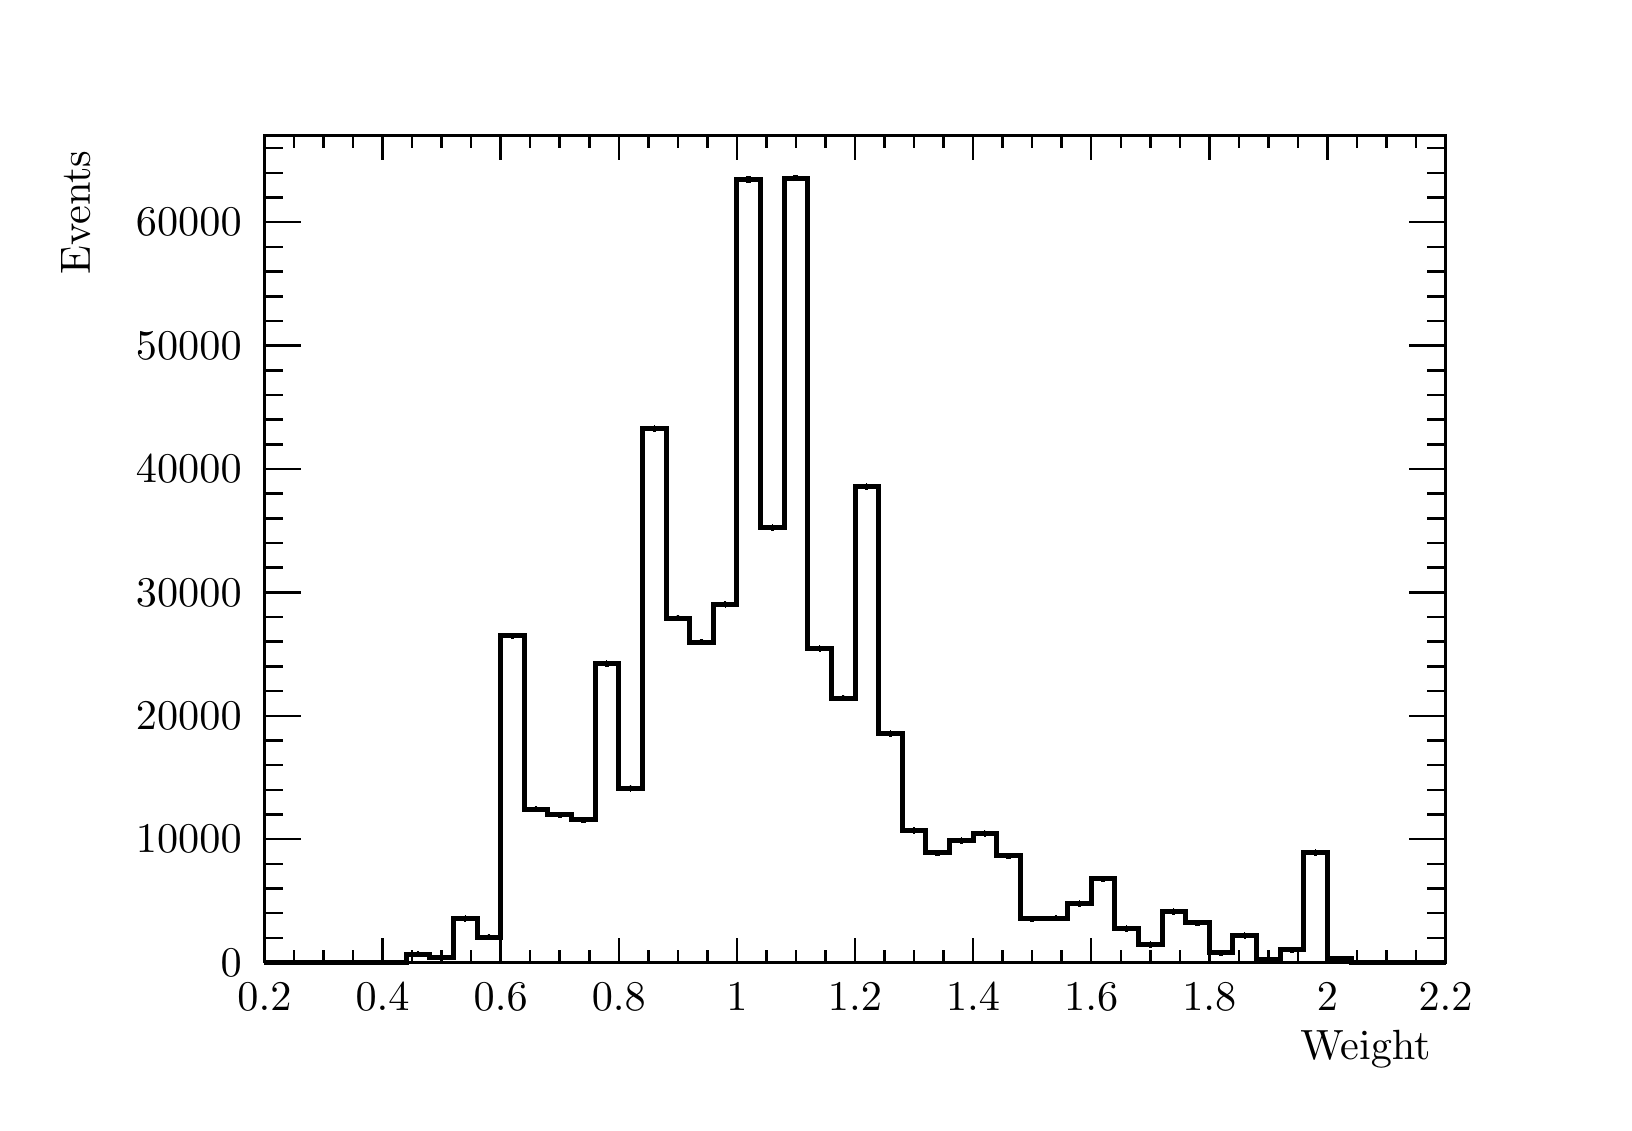
\begin{tikzpicture}
\pgfdeclareplotmark{cross} {
\pgfpathmoveto{\pgfpoint{-0.3\pgfplotmarksize}{\pgfplotmarksize}}
\pgfpathlineto{\pgfpoint{+0.3\pgfplotmarksize}{\pgfplotmarksize}}
\pgfpathlineto{\pgfpoint{+0.3\pgfplotmarksize}{0.3\pgfplotmarksize}}
\pgfpathlineto{\pgfpoint{+1\pgfplotmarksize}{0.3\pgfplotmarksize}}
\pgfpathlineto{\pgfpoint{+1\pgfplotmarksize}{-0.3\pgfplotmarksize}}
\pgfpathlineto{\pgfpoint{+0.3\pgfplotmarksize}{-0.3\pgfplotmarksize}}
\pgfpathlineto{\pgfpoint{+0.3\pgfplotmarksize}{-1.\pgfplotmarksize}}
\pgfpathlineto{\pgfpoint{-0.3\pgfplotmarksize}{-1.\pgfplotmarksize}}
\pgfpathlineto{\pgfpoint{-0.3\pgfplotmarksize}{-0.3\pgfplotmarksize}}
\pgfpathlineto{\pgfpoint{-1.\pgfplotmarksize}{-0.3\pgfplotmarksize}}
\pgfpathlineto{\pgfpoint{-1.\pgfplotmarksize}{0.3\pgfplotmarksize}}
\pgfpathlineto{\pgfpoint{-0.3\pgfplotmarksize}{0.3\pgfplotmarksize}}
\pgfpathclose
\pgfusepathqstroke
}
\pgfdeclareplotmark{cross*} {
\pgfpathmoveto{\pgfpoint{-0.3\pgfplotmarksize}{\pgfplotmarksize}}
\pgfpathlineto{\pgfpoint{+0.3\pgfplotmarksize}{\pgfplotmarksize}}
\pgfpathlineto{\pgfpoint{+0.3\pgfplotmarksize}{0.3\pgfplotmarksize}}
\pgfpathlineto{\pgfpoint{+1\pgfplotmarksize}{0.3\pgfplotmarksize}}
\pgfpathlineto{\pgfpoint{+1\pgfplotmarksize}{-0.3\pgfplotmarksize}}
\pgfpathlineto{\pgfpoint{+0.3\pgfplotmarksize}{-0.3\pgfplotmarksize}}
\pgfpathlineto{\pgfpoint{+0.3\pgfplotmarksize}{-1.\pgfplotmarksize}}
\pgfpathlineto{\pgfpoint{-0.3\pgfplotmarksize}{-1.\pgfplotmarksize}}
\pgfpathlineto{\pgfpoint{-0.3\pgfplotmarksize}{-0.3\pgfplotmarksize}}
\pgfpathlineto{\pgfpoint{-1.\pgfplotmarksize}{-0.3\pgfplotmarksize}}
\pgfpathlineto{\pgfpoint{-1.\pgfplotmarksize}{0.3\pgfplotmarksize}}
\pgfpathlineto{\pgfpoint{-0.3\pgfplotmarksize}{0.3\pgfplotmarksize}}
\pgfpathclose
\pgfusepathqfillstroke
}
\pgfdeclareplotmark{newstar} {
\pgfpathmoveto{\pgfqpoint{0pt}{\pgfplotmarksize}}
\pgfpathlineto{\pgfqpointpolar{44}{0.5\pgfplotmarksize}}
\pgfpathlineto{\pgfqpointpolar{18}{\pgfplotmarksize}}
\pgfpathlineto{\pgfqpointpolar{-20}{0.5\pgfplotmarksize}}
\pgfpathlineto{\pgfqpointpolar{-54}{\pgfplotmarksize}}
\pgfpathlineto{\pgfqpointpolar{-90}{0.5\pgfplotmarksize}}
\pgfpathlineto{\pgfqpointpolar{234}{\pgfplotmarksize}}
\pgfpathlineto{\pgfqpointpolar{198}{0.5\pgfplotmarksize}}
\pgfpathlineto{\pgfqpointpolar{162}{\pgfplotmarksize}}
\pgfpathlineto{\pgfqpointpolar{134}{0.5\pgfplotmarksize}}
\pgfpathclose
\pgfusepathqstroke
}
\pgfdeclareplotmark{newstar*} {
\pgfpathmoveto{\pgfqpoint{0pt}{\pgfplotmarksize}}
\pgfpathlineto{\pgfqpointpolar{44}{0.5\pgfplotmarksize}}
\pgfpathlineto{\pgfqpointpolar{18}{\pgfplotmarksize}}
\pgfpathlineto{\pgfqpointpolar{-20}{0.5\pgfplotmarksize}}
\pgfpathlineto{\pgfqpointpolar{-54}{\pgfplotmarksize}}
\pgfpathlineto{\pgfqpointpolar{-90}{0.5\pgfplotmarksize}}
\pgfpathlineto{\pgfqpointpolar{234}{\pgfplotmarksize}}
\pgfpathlineto{\pgfqpointpolar{198}{0.5\pgfplotmarksize}}
\pgfpathlineto{\pgfqpointpolar{162}{\pgfplotmarksize}}
\pgfpathlineto{\pgfqpointpolar{134}{0.5\pgfplotmarksize}}
\pgfpathclose
\pgfusepathqfillstroke
}
\definecolor{c}{rgb}{1,1,1};
\draw [color=c, fill=c] (0,0) rectangle (20,13.639);
\draw [color=c, fill=c] (3,1.77307) rectangle (18,12.2751);
\definecolor{c}{rgb}{0,0,0};
\draw [c,line width=0.9] (3,1.77307) -- (3,12.2751) -- (18,12.2751) -- (18,1.77307) -- (3,1.77307);
\definecolor{c}{rgb}{1,1,1};
\draw [color=c, fill=c] (3,1.77307) rectangle (18,12.2751);
\definecolor{c}{rgb}{0,0,0};
\draw [c,line width=0.9] (3,1.77307) -- (3,12.2751) -- (18,12.2751) -- (18,1.77307) -- (3,1.77307);
\draw [c,line width=1.8] (4.95,1.87523) -- (4.95,1.87931);
\draw [c,line width=1.8] (4.95,1.87931) -- (4.95,1.88339);
\foreach \P in {(4.95,1.87931)}{\draw[mark options={color=c,fill=c},mark size=2.402402pt, line width=0.000000pt, mark=*,mark size=1pt] plot coordinates {\P};}
\draw [c,line width=1.8] (5.25,1.83063) -- (5.25,1.83371);
\draw [c,line width=1.8] (5.25,1.83371) -- (5.25,1.83679);
\foreach \P in {(5.25,1.83371)}{\draw[mark options={color=c,fill=c},mark size=2.402402pt, line width=0.000000pt, mark=*,mark size=1pt] plot coordinates {\P};}
\draw [c,line width=1.8] (5.55,2.32328) -- (5.55,2.33264);
\draw [c,line width=1.8] (5.55,2.33264) -- (5.55,2.34201);
\foreach \P in {(5.55,2.33264)}{\draw[mark options={color=c,fill=c},mark size=2.402402pt, line width=0.000000pt, mark=*,mark size=1pt] plot coordinates {\P};}
\draw [c,line width=1.8] (5.85,2.08845) -- (5.85,2.09556);
\draw [c,line width=1.8] (5.85,2.09556) -- (5.85,2.10266);
\foreach \P in {(5.85,2.09556)}{\draw[mark options={color=c,fill=c},mark size=2.402402pt, line width=0.000000pt, mark=*,mark size=1pt] plot coordinates {\P};}
\draw [c,line width=1.8] (6.15,5.897) -- (6.15,5.9225);
\draw [c,line width=1.8] (6.15,5.9225) -- (6.15,5.948);
\foreach \P in {(6.15,5.9225)}{\draw[mark options={color=c,fill=c},mark size=2.402402pt, line width=0.000000pt, mark=*,mark size=1pt] plot coordinates {\P};}
\draw [c,line width=1.8] (6.45,3.70323) -- (6.45,3.7207);
\draw [c,line width=1.8] (6.45,3.7207) -- (6.45,3.73817);
\foreach \P in {(6.45,3.7207)}{\draw[mark options={color=c,fill=c},mark size=2.402402pt, line width=0.000000pt, mark=*,mark size=1pt] plot coordinates {\P};}
\draw [c,line width=1.8] (6.75,3.63132) -- (6.75,3.64846);
\draw [c,line width=1.8] (6.75,3.64846) -- (6.75,3.6656);
\foreach \P in {(6.75,3.64846)}{\draw[mark options={color=c,fill=c},mark size=2.402402pt, line width=0.000000pt, mark=*,mark size=1pt] plot coordinates {\P};}
\draw [c,line width=1.8] (7.05,3.56674) -- (7.05,3.58359);
\draw [c,line width=1.8] (7.05,3.58359) -- (7.05,3.60043);
\foreach \P in {(7.05,3.58359)}{\draw[mark options={color=c,fill=c},mark size=2.402402pt, line width=0.000000pt, mark=*,mark size=1pt] plot coordinates {\P};}
\draw [c,line width=1.8] (7.35,5.54412) -- (7.35,5.56851);
\draw [c,line width=1.8] (7.35,5.56851) -- (7.35,5.5929);
\foreach \P in {(7.35,5.56851)}{\draw[mark options={color=c,fill=c},mark size=2.402402pt, line width=0.000000pt, mark=*,mark size=1pt] plot coordinates {\P};}
\draw [c,line width=1.8] (7.65,3.96799) -- (7.65,3.98662);
\draw [c,line width=1.8] (7.65,3.98662) -- (7.65,4.00524);
\foreach \P in {(7.65,3.98662)}{\draw[mark options={color=c,fill=c},mark size=2.402402pt, line width=0.000000pt, mark=*,mark size=1pt] plot coordinates {\P};}
\draw [c,line width=1.8] (7.95,8.52091) -- (7.95,8.5535);
\draw [c,line width=1.8] (7.95,8.5535) -- (7.95,8.5861);
\foreach \P in {(7.95,8.5535)}{\draw[mark options={color=c,fill=c},mark size=2.402402pt, line width=0.000000pt, mark=*,mark size=1pt] plot coordinates {\P};}
\draw [c,line width=1.8] (8.25,6.12243) -- (8.25,6.14862);
\draw [c,line width=1.8] (8.25,6.14862) -- (8.25,6.1748);
\foreach \P in {(8.25,6.14862)}{\draw[mark options={color=c,fill=c},mark size=2.402402pt, line width=0.000000pt, mark=*,mark size=1pt] plot coordinates {\P};}
\draw [c,line width=1.8] (8.55,5.81842) -- (8.55,5.84368);
\draw [c,line width=1.8] (8.55,5.84368) -- (8.55,5.86893);
\foreach \P in {(8.55,5.84368)}{\draw[mark options={color=c,fill=c},mark size=2.402402pt, line width=0.000000pt, mark=*,mark size=1pt] plot coordinates {\P};}
\draw [c,line width=1.8] (8.85,6.29679) -- (8.85,6.3235);
\draw [c,line width=1.8] (8.85,6.3235) -- (8.85,6.3502);
\foreach \P in {(8.85,6.3235)}{\draw[mark options={color=c,fill=c},mark size=2.402402pt, line width=0.000000pt, mark=*,mark size=1pt] plot coordinates {\P};}
\draw [c,line width=1.8] (9.15,11.6789) -- (9.15,11.7184);
\draw [c,line width=1.8] (9.15,11.7184) -- (9.15,11.7579);
\foreach \P in {(9.15,11.7184)}{\draw[mark options={color=c,fill=c},mark size=2.402402pt, line width=0.000000pt, mark=*,mark size=1pt] plot coordinates {\P};}
\draw [c,line width=1.8] (9.45,7.26703) -- (9.45,7.29645);
\draw [c,line width=1.8] (9.45,7.29645) -- (9.45,7.32587);
\foreach \P in {(9.45,7.29645)}{\draw[mark options={color=c,fill=c},mark size=2.402402pt, line width=0.000000pt, mark=*,mark size=1pt] plot coordinates {\P};}
\draw [c,line width=1.8] (9.75,11.696) -- (9.75,11.7355);
\draw [c,line width=1.8] (9.75,11.7355) -- (9.75,11.775);
\foreach \P in {(9.75,11.7355)}{\draw[mark options={color=c,fill=c},mark size=2.402402pt, line width=0.000000pt, mark=*,mark size=1pt] plot coordinates {\P};}
\draw [c,line width=1.8] (10.05,5.73719) -- (10.05,5.76219);
\draw [c,line width=1.8] (10.05,5.76219) -- (10.05,5.7872);
\foreach \P in {(10.05,5.76219)}{\draw[mark options={color=c,fill=c},mark size=2.402402pt, line width=0.000000pt, mark=*,mark size=1pt] plot coordinates {\P};}
\draw [c,line width=1.8] (10.35,5.10838) -- (10.35,5.13132);
\draw [c,line width=1.8] (10.35,5.13132) -- (10.35,5.15426);
\foreach \P in {(10.35,5.13132)}{\draw[mark options={color=c,fill=c},mark size=2.402402pt, line width=0.000000pt, mark=*,mark size=1pt] plot coordinates {\P};}
\draw [c,line width=1.8] (10.65,7.78702) -- (10.65,7.81779);
\draw [c,line width=1.8] (10.65,7.81779) -- (10.65,7.84857);
\foreach \P in {(10.65,7.81779)}{\draw[mark options={color=c,fill=c},mark size=2.402402pt, line width=0.000000pt, mark=*,mark size=1pt] plot coordinates {\P};}
\draw [c,line width=1.8] (10.95,4.65852) -- (10.95,4.67986);
\draw [c,line width=1.8] (10.95,4.67986) -- (10.95,4.7012);
\foreach \P in {(10.95,4.67986)}{\draw[mark options={color=c,fill=c},mark size=2.402402pt, line width=0.000000pt, mark=*,mark size=1pt] plot coordinates {\P};}
\draw [c,line width=1.8] (11.25,3.4362) -- (11.25,3.45243);
\draw [c,line width=1.8] (11.25,3.45243) -- (11.25,3.46865);
\foreach \P in {(11.25,3.45243)}{\draw[mark options={color=c,fill=c},mark size=2.402402pt, line width=0.000000pt, mark=*,mark size=1pt] plot coordinates {\P};}
\draw [c,line width=1.8] (11.55,3.15042) -- (11.55,3.16519);
\draw [c,line width=1.8] (11.55,3.16519) -- (11.55,3.17996);
\foreach \P in {(11.55,3.16519)}{\draw[mark options={color=c,fill=c},mark size=2.402402pt, line width=0.000000pt, mark=*,mark size=1pt] plot coordinates {\P};}
\draw [c,line width=1.8] (11.85,3.30663) -- (11.85,3.32221);
\draw [c,line width=1.8] (11.85,3.32221) -- (11.85,3.33779);
\foreach \P in {(11.85,3.32221)}{\draw[mark options={color=c,fill=c},mark size=2.402402pt, line width=0.000000pt, mark=*,mark size=1pt] plot coordinates {\P};}
\draw [c,line width=1.8] (12.15,3.39675) -- (12.15,3.41278);
\draw [c,line width=1.8] (12.15,3.41278) -- (12.15,3.42881);
\foreach \P in {(12.15,3.41278)}{\draw[mark options={color=c,fill=c},mark size=2.402402pt, line width=0.000000pt, mark=*,mark size=1pt] plot coordinates {\P};}
\draw [c,line width=1.8] (12.45,3.11271) -- (12.45,3.12727);
\draw [c,line width=1.8] (12.45,3.12727) -- (12.45,3.14184);
\foreach \P in {(12.45,3.12727)}{\draw[mark options={color=c,fill=c},mark size=2.402402pt, line width=0.000000pt, mark=*,mark size=1pt] plot coordinates {\P};}
\draw [c,line width=1.8] (12.75,2.31738) -- (12.75,2.32669);
\draw [c,line width=1.8] (12.75,2.32669) -- (12.75,2.336);
\foreach \P in {(12.75,2.32669)}{\draw[mark options={color=c,fill=c},mark size=2.402402pt, line width=0.000000pt, mark=*,mark size=1pt] plot coordinates {\P};}
\draw [c,line width=1.8] (13.05,2.32654) -- (13.05,2.33593);
\draw [c,line width=1.8] (13.05,2.33593) -- (13.05,2.34533);
\foreach \P in {(13.05,2.33593)}{\draw[mark options={color=c,fill=c},mark size=2.402402pt, line width=0.000000pt, mark=*,mark size=1pt] plot coordinates {\P};}
\draw [c,line width=1.8] (13.35,2.50986) -- (13.35,2.52068);
\draw [c,line width=1.8] (13.35,2.52068) -- (13.35,2.53151);
\foreach \P in {(13.35,2.52068)}{\draw[mark options={color=c,fill=c},mark size=2.402402pt, line width=0.000000pt, mark=*,mark size=1pt] plot coordinates {\P};}
\draw [c,line width=1.8] (13.65,2.82384) -- (13.65,2.83675);
\draw [c,line width=1.8] (13.65,2.83675) -- (13.65,2.84966);
\foreach \P in {(13.65,2.83675)}{\draw[mark options={color=c,fill=c},mark size=2.402402pt, line width=0.000000pt, mark=*,mark size=1pt] plot coordinates {\P};}
\draw [c,line width=1.8] (13.95,2.19671) -- (13.95,2.20493);
\draw [c,line width=1.8] (13.95,2.20493) -- (13.95,2.21316);
\foreach \P in {(13.95,2.20493)}{\draw[mark options={color=c,fill=c},mark size=2.402402pt, line width=0.000000pt, mark=*,mark size=1pt] plot coordinates {\P};}
\draw [c,line width=1.8] (14.25,1.99478) -- (14.25,2.00075);
\draw [c,line width=1.8] (14.25,2.00075) -- (14.25,2.00673);
\foreach \P in {(14.25,2.00075)}{\draw[mark options={color=c,fill=c},mark size=2.402402pt, line width=0.000000pt, mark=*,mark size=1pt] plot coordinates {\P};}
\draw [c,line width=1.8] (14.55,2.40986) -- (14.55,2.41993);
\draw [c,line width=1.8] (14.55,2.41993) -- (14.55,2.42999);
\foreach \P in {(14.55,2.41993)}{\draw[mark options={color=c,fill=c},mark size=2.402402pt, line width=0.000000pt, mark=*,mark size=1pt] plot coordinates {\P};}
\draw [c,line width=1.8] (14.85,2.26735) -- (14.85,2.27623);
\draw [c,line width=1.8] (14.85,2.27623) -- (14.85,2.28511);
\foreach \P in {(14.85,2.27623)}{\draw[mark options={color=c,fill=c},mark size=2.402402pt, line width=0.000000pt, mark=*,mark size=1pt] plot coordinates {\P};}
\draw [c,line width=1.8] (15.15,1.89107) -- (15.15,1.89545);
\draw [c,line width=1.8] (15.15,1.89545) -- (15.15,1.89983);
\foreach \P in {(15.15,1.89545)}{\draw[mark options={color=c,fill=c},mark size=2.402402pt, line width=0.000000pt, mark=*,mark size=1pt] plot coordinates {\P};}
\draw [c,line width=1.8] (15.45,2.10937) -- (15.45,2.11671);
\draw [c,line width=1.8] (15.45,2.11671) -- (15.45,2.12405);
\foreach \P in {(15.45,2.11671)}{\draw[mark options={color=c,fill=c},mark size=2.402402pt, line width=0.000000pt, mark=*,mark size=1pt] plot coordinates {\P};}
\draw [c,line width=1.8] (15.75,1.81052) -- (15.75,1.81302);
\draw [c,line width=1.8] (15.75,1.81302) -- (15.75,1.81553);
\foreach \P in {(15.75,1.81302)}{\draw[mark options={color=c,fill=c},mark size=2.402402pt, line width=0.000000pt, mark=*,mark size=1pt] plot coordinates {\P};}
\draw [c,line width=1.8] (16.05,1.92759) -- (16.05,1.93259);
\draw [c,line width=1.8] (16.05,1.93259) -- (16.05,1.93759);
\foreach \P in {(16.05,1.93259)}{\draw[mark options={color=c,fill=c},mark size=2.402402pt, line width=0.000000pt, mark=*,mark size=1pt] plot coordinates {\P};}
\draw [c,line width=1.8] (16.35,3.1551) -- (16.35,3.1699);
\draw [c,line width=1.8] (16.35,3.1699) -- (16.35,3.18469);
\foreach \P in {(16.35,3.1699)}{\draw[mark options={color=c,fill=c},mark size=2.402402pt, line width=0.000000pt, mark=*,mark size=1pt] plot coordinates {\P};}
\draw [c,line width=1.8] (16.65,1.81675) -- (16.65,1.81945);
\draw [c,line width=1.8] (16.65,1.81945) -- (16.65,1.82215);
\foreach \P in {(16.65,1.81945)}{\draw[mark options={color=c,fill=c},mark size=2.402402pt, line width=0.000000pt, mark=*,mark size=1pt] plot coordinates {\P};}
\draw [c,line width=1.8] (3,1.77307) -- (3.3,1.77307) -- (3.3,1.77307) -- (3.6,1.77307) -- (3.6,1.77307) -- (3.9,1.77307) -- (3.9,1.77307) -- (4.2,1.77307) -- (4.2,1.77307) -- (4.5,1.77307) -- (4.5,1.77307) -- (4.8,1.77307) -- (4.8,1.87931) --
 (5.1,1.87931) -- (5.1,1.83371) -- (5.4,1.83371) -- (5.4,2.33264) -- (5.7,2.33264) -- (5.7,2.09556) -- (6,2.09556) -- (6,5.9225) -- (6.3,5.9225) -- (6.3,3.7207) -- (6.6,3.7207) -- (6.6,3.64846) -- (6.9,3.64846) -- (6.9,3.58359) -- (7.2,3.58359) --
 (7.2,5.56851) -- (7.5,5.56851) -- (7.5,3.98662) -- (7.8,3.98662) -- (7.8,8.5535) -- (8.1,8.5535) -- (8.1,6.14862) -- (8.4,6.14862) -- (8.4,5.84368) -- (8.7,5.84368) -- (8.7,6.3235) -- (9,6.3235) -- (9,11.7184) -- (9.3,11.7184) -- (9.3,7.29645) --
 (9.6,7.29645) -- (9.6,11.7355) -- (9.9,11.7355) -- (9.9,5.76219) -- (10.2,5.76219) -- (10.2,5.13132) -- (10.5,5.13132) -- (10.5,7.81779) -- (10.8,7.81779) -- (10.8,4.67986) -- (11.1,4.67986) -- (11.1,3.45243) -- (11.4,3.45243) -- (11.4,3.16519) --
 (11.7,3.16519) -- (11.7,3.32221) -- (12,3.32221) -- (12,3.41278) -- (12.3,3.41278) -- (12.3,3.12727) -- (12.6,3.12727) -- (12.6,2.32669) -- (12.9,2.32669) -- (12.9,2.33593) -- (13.2,2.33593) -- (13.2,2.52068) -- (13.5,2.52068) -- (13.5,2.83675) --
 (13.8,2.83675) -- (13.8,2.20493) -- (14.1,2.20493) -- (14.1,2.00075) -- (14.4,2.00075) -- (14.4,2.41993) -- (14.7,2.41993) -- (14.7,2.27623) -- (15,2.27623) -- (15,1.89545) -- (15.3,1.89545) -- (15.3,2.11671) -- (15.6,2.11671) -- (15.6,1.81302) --
 (15.9,1.81302) -- (15.9,1.93259) -- (16.2,1.93259) -- (16.2,3.1699) -- (16.5,3.1699) -- (16.5,1.81945) -- (16.8,1.81945) -- (16.8,1.77307) -- (17.1,1.77307) -- (17.1,1.77307) -- (17.4,1.77307) -- (17.4,1.77307) -- (17.7,1.77307) -- (17.7,1.77307) --
 (18,1.77307);
\draw [c,line width=0.9] (3,1.77307) -- (18,1.77307);
\draw [c,line width=0.9] (3,2.07994) -- (3,1.77307);
\draw [c,line width=0.9] (3.375,1.9265) -- (3.375,1.77307);
\draw [c,line width=0.9] (3.75,1.9265) -- (3.75,1.77307);
\draw [c,line width=0.9] (4.125,1.9265) -- (4.125,1.77307);
\draw [c,line width=0.9] (4.5,2.07994) -- (4.5,1.77307);
\draw [c,line width=0.9] (4.875,1.9265) -- (4.875,1.77307);
\draw [c,line width=0.9] (5.25,1.9265) -- (5.25,1.77307);
\draw [c,line width=0.9] (5.625,1.9265) -- (5.625,1.77307);
\draw [c,line width=0.9] (6,2.07994) -- (6,1.77307);
\draw [c,line width=0.9] (6.375,1.9265) -- (6.375,1.77307);
\draw [c,line width=0.9] (6.75,1.9265) -- (6.75,1.77307);
\draw [c,line width=0.9] (7.125,1.9265) -- (7.125,1.77307);
\draw [c,line width=0.9] (7.5,2.07994) -- (7.5,1.77307);
\draw [c,line width=0.9] (7.875,1.9265) -- (7.875,1.77307);
\draw [c,line width=0.9] (8.25,1.9265) -- (8.25,1.77307);
\draw [c,line width=0.9] (8.625,1.9265) -- (8.625,1.77307);
\draw [c,line width=0.9] (9,2.07994) -- (9,1.77307);
\draw [c,line width=0.9] (9.375,1.9265) -- (9.375,1.77307);
\draw [c,line width=0.9] (9.75,1.9265) -- (9.75,1.77307);
\draw [c,line width=0.9] (10.125,1.9265) -- (10.125,1.77307);
\draw [c,line width=0.9] (10.5,2.07994) -- (10.5,1.77307);
\draw [c,line width=0.9] (10.875,1.9265) -- (10.875,1.77307);
\draw [c,line width=0.9] (11.25,1.9265) -- (11.25,1.77307);
\draw [c,line width=0.9] (11.625,1.9265) -- (11.625,1.77307);
\draw [c,line width=0.9] (12,2.07994) -- (12,1.77307);
\draw [c,line width=0.9] (12.375,1.9265) -- (12.375,1.77307);
\draw [c,line width=0.9] (12.75,1.9265) -- (12.75,1.77307);
\draw [c,line width=0.9] (13.125,1.9265) -- (13.125,1.77307);
\draw [c,line width=0.9] (13.5,2.07994) -- (13.5,1.77307);
\draw [c,line width=0.9] (13.875,1.9265) -- (13.875,1.77307);
\draw [c,line width=0.9] (14.25,1.9265) -- (14.25,1.77307);
\draw [c,line width=0.9] (14.625,1.9265) -- (14.625,1.77307);
\draw [c,line width=0.9] (15,2.07994) -- (15,1.77307);
\draw [c,line width=0.9] (15.375,1.9265) -- (15.375,1.77307);
\draw [c,line width=0.9] (15.75,1.9265) -- (15.75,1.77307);
\draw [c,line width=0.9] (16.125,1.9265) -- (16.125,1.77307);
\draw [c,line width=0.9] (16.5,2.07994) -- (16.5,1.77307);
\draw [c,line width=0.9] (16.875,1.9265) -- (16.875,1.77307);
\draw [c,line width=0.9] (17.25,1.9265) -- (17.25,1.77307);
\draw [c,line width=0.9] (17.625,1.9265) -- (17.625,1.77307);
\draw [c,line width=0.9] (18,2.07994) -- (18,1.77307);
\draw [anchor=base] (3,1.15931) node[scale=1.52731, color=c, rotate=0]{0.2};
\draw [anchor=base] (4.5,1.15931) node[scale=1.52731, color=c, rotate=0]{0.4};
\draw [anchor=base] (6,1.15931) node[scale=1.52731, color=c, rotate=0]{0.6};
\draw [anchor=base] (7.5,1.15931) node[scale=1.52731, color=c, rotate=0]{0.8};
\draw [anchor=base] (9,1.15931) node[scale=1.52731, color=c, rotate=0]{1};
\draw [anchor=base] (10.5,1.15931) node[scale=1.52731, color=c, rotate=0]{1.2};
\draw [anchor=base] (12,1.15931) node[scale=1.52731, color=c, rotate=0]{1.4};
\draw [anchor=base] (13.5,1.15931) node[scale=1.52731, color=c, rotate=0]{1.6};
\draw [anchor=base] (15,1.15931) node[scale=1.52731, color=c, rotate=0]{1.8};
\draw [anchor=base] (16.5,1.15931) node[scale=1.52731, color=c, rotate=0]{2};
\draw [anchor=base] (18,1.15931) node[scale=1.52731, color=c, rotate=0]{2.2};
\draw [anchor= east] (18,0.681948) node[scale=1.52731, color=c, rotate=0]{ Weight};
\draw [c,line width=0.9] (3,12.2751) -- (18,12.2751);
\draw [c,line width=0.9] (3,11.9682) -- (3,12.2751);
\draw [c,line width=0.9] (3.375,12.1216) -- (3.375,12.2751);
\draw [c,line width=0.9] (3.75,12.1216) -- (3.75,12.2751);
\draw [c,line width=0.9] (4.125,12.1216) -- (4.125,12.2751);
\draw [c,line width=0.9] (4.5,11.9682) -- (4.5,12.2751);
\draw [c,line width=0.9] (4.875,12.1216) -- (4.875,12.2751);
\draw [c,line width=0.9] (5.25,12.1216) -- (5.25,12.2751);
\draw [c,line width=0.9] (5.625,12.1216) -- (5.625,12.2751);
\draw [c,line width=0.9] (6,11.9682) -- (6,12.2751);
\draw [c,line width=0.9] (6.375,12.1216) -- (6.375,12.2751);
\draw [c,line width=0.9] (6.75,12.1216) -- (6.75,12.2751);
\draw [c,line width=0.9] (7.125,12.1216) -- (7.125,12.2751);
\draw [c,line width=0.9] (7.5,11.9682) -- (7.5,12.2751);
\draw [c,line width=0.9] (7.875,12.1216) -- (7.875,12.2751);
\draw [c,line width=0.9] (8.25,12.1216) -- (8.25,12.2751);
\draw [c,line width=0.9] (8.625,12.1216) -- (8.625,12.2751);
\draw [c,line width=0.9] (9,11.9682) -- (9,12.2751);
\draw [c,line width=0.9] (9.375,12.1216) -- (9.375,12.2751);
\draw [c,line width=0.9] (9.75,12.1216) -- (9.75,12.2751);
\draw [c,line width=0.9] (10.125,12.1216) -- (10.125,12.2751);
\draw [c,line width=0.9] (10.5,11.9682) -- (10.5,12.2751);
\draw [c,line width=0.9] (10.875,12.1216) -- (10.875,12.2751);
\draw [c,line width=0.9] (11.25,12.1216) -- (11.25,12.2751);
\draw [c,line width=0.9] (11.625,12.1216) -- (11.625,12.2751);
\draw [c,line width=0.9] (12,11.9682) -- (12,12.2751);
\draw [c,line width=0.9] (12.375,12.1216) -- (12.375,12.2751);
\draw [c,line width=0.9] (12.75,12.1216) -- (12.75,12.2751);
\draw [c,line width=0.9] (13.125,12.1216) -- (13.125,12.2751);
\draw [c,line width=0.9] (13.5,11.9682) -- (13.5,12.2751);
\draw [c,line width=0.9] (13.875,12.1216) -- (13.875,12.2751);
\draw [c,line width=0.9] (14.25,12.1216) -- (14.25,12.2751);
\draw [c,line width=0.9] (14.625,12.1216) -- (14.625,12.2751);
\draw [c,line width=0.9] (15,11.9682) -- (15,12.2751);
\draw [c,line width=0.9] (15.375,12.1216) -- (15.375,12.2751);
\draw [c,line width=0.9] (15.75,12.1216) -- (15.75,12.2751);
\draw [c,line width=0.9] (16.125,12.1216) -- (16.125,12.2751);
\draw [c,line width=0.9] (16.5,11.9682) -- (16.5,12.2751);
\draw [c,line width=0.9] (16.875,12.1216) -- (16.875,12.2751);
\draw [c,line width=0.9] (17.25,12.1216) -- (17.25,12.2751);
\draw [c,line width=0.9] (17.625,12.1216) -- (17.625,12.2751);
\draw [c,line width=0.9] (18,11.9682) -- (18,12.2751);
\draw [c,line width=0.9] (3,1.77307) -- (3,12.2751);
\draw [c,line width=0.9] (3.462,1.77307) -- (3,1.77307);
\draw [c,line width=0.9] (3.231,2.08647) -- (3,2.08647);
\draw [c,line width=0.9] (3.231,2.39987) -- (3,2.39987);
\draw [c,line width=0.9] (3.231,2.71327) -- (3,2.71327);
\draw [c,line width=0.9] (3.231,3.02667) -- (3,3.02667);
\draw [c,line width=0.9] (3.462,3.34007) -- (3,3.34007);
\draw [c,line width=0.9] (3.231,3.65347) -- (3,3.65347);
\draw [c,line width=0.9] (3.231,3.96687) -- (3,3.96687);
\draw [c,line width=0.9] (3.231,4.28028) -- (3,4.28028);
\draw [c,line width=0.9] (3.231,4.59368) -- (3,4.59368);
\draw [c,line width=0.9] (3.462,4.90708) -- (3,4.90708);
\draw [c,line width=0.9] (3.231,5.22048) -- (3,5.22048);
\draw [c,line width=0.9] (3.231,5.53388) -- (3,5.53388);
\draw [c,line width=0.9] (3.231,5.84728) -- (3,5.84728);
\draw [c,line width=0.9] (3.231,6.16068) -- (3,6.16068);
\draw [c,line width=0.9] (3.462,6.47408) -- (3,6.47408);
\draw [c,line width=0.9] (3.231,6.78749) -- (3,6.78749);
\draw [c,line width=0.9] (3.231,7.10089) -- (3,7.10089);
\draw [c,line width=0.9] (3.231,7.41429) -- (3,7.41429);
\draw [c,line width=0.9] (3.231,7.72769) -- (3,7.72769);
\draw [c,line width=0.9] (3.462,8.04109) -- (3,8.04109);
\draw [c,line width=0.9] (3.231,8.35449) -- (3,8.35449);
\draw [c,line width=0.9] (3.231,8.66789) -- (3,8.66789);
\draw [c,line width=0.9] (3.231,8.98129) -- (3,8.98129);
\draw [c,line width=0.9] (3.231,9.2947) -- (3,9.2947);
\draw [c,line width=0.9] (3.462,9.6081) -- (3,9.6081);
\draw [c,line width=0.9] (3.231,9.9215) -- (3,9.9215);
\draw [c,line width=0.9] (3.231,10.2349) -- (3,10.2349);
\draw [c,line width=0.9] (3.231,10.5483) -- (3,10.5483);
\draw [c,line width=0.9] (3.231,10.8617) -- (3,10.8617);
\draw [c,line width=0.9] (3.462,11.1751) -- (3,11.1751);
\draw [c,line width=0.9] (3.462,11.1751) -- (3,11.1751);
\draw [c,line width=0.9] (3.231,11.4885) -- (3,11.4885);
\draw [c,line width=0.9] (3.231,11.8019) -- (3,11.8019);
\draw [c,line width=0.9] (3.231,12.1153) -- (3,12.1153);
\draw [anchor= east] (2.9,1.77307) node[scale=1.52731, color=c, rotate=0]{0};
\draw [anchor= east] (2.9,3.34007) node[scale=1.52731, color=c, rotate=0]{10000};
\draw [anchor= east] (2.9,4.90708) node[scale=1.52731, color=c, rotate=0]{20000};
\draw [anchor= east] (2.9,6.47408) node[scale=1.52731, color=c, rotate=0]{30000};
\draw [anchor= east] (2.9,8.04109) node[scale=1.52731, color=c, rotate=0]{40000};
\draw [anchor= east] (2.9,9.6081) node[scale=1.52731, color=c, rotate=0]{50000};
\draw [anchor= east] (2.9,11.1751) node[scale=1.52731, color=c, rotate=0]{60000};
\draw [anchor= east] (0.6,12.2751) node[scale=1.52731, color=c, rotate=90]{ Events};
\draw [c,line width=0.9] (18,1.77307) -- (18,12.2751);
\draw [c,line width=0.9] (17.538,1.77307) -- (18,1.77307);
\draw [c,line width=0.9] (17.769,2.08647) -- (18,2.08647);
\draw [c,line width=0.9] (17.769,2.39987) -- (18,2.39987);
\draw [c,line width=0.9] (17.769,2.71327) -- (18,2.71327);
\draw [c,line width=0.9] (17.769,3.02667) -- (18,3.02667);
\draw [c,line width=0.9] (17.538,3.34007) -- (18,3.34007);
\draw [c,line width=0.9] (17.769,3.65347) -- (18,3.65347);
\draw [c,line width=0.9] (17.769,3.96687) -- (18,3.96687);
\draw [c,line width=0.9] (17.769,4.28028) -- (18,4.28028);
\draw [c,line width=0.9] (17.769,4.59368) -- (18,4.59368);
\draw [c,line width=0.9] (17.538,4.90708) -- (18,4.90708);
\draw [c,line width=0.9] (17.769,5.22048) -- (18,5.22048);
\draw [c,line width=0.9] (17.769,5.53388) -- (18,5.53388);
\draw [c,line width=0.9] (17.769,5.84728) -- (18,5.84728);
\draw [c,line width=0.9] (17.769,6.16068) -- (18,6.16068);
\draw [c,line width=0.9] (17.538,6.47408) -- (18,6.47408);
\draw [c,line width=0.9] (17.769,6.78749) -- (18,6.78749);
\draw [c,line width=0.9] (17.769,7.10089) -- (18,7.10089);
\draw [c,line width=0.9] (17.769,7.41429) -- (18,7.41429);
\draw [c,line width=0.9] (17.769,7.72769) -- (18,7.72769);
\draw [c,line width=0.9] (17.538,8.04109) -- (18,8.04109);
\draw [c,line width=0.9] (17.769,8.35449) -- (18,8.35449);
\draw [c,line width=0.9] (17.769,8.66789) -- (18,8.66789);
\draw [c,line width=0.9] (17.769,8.98129) -- (18,8.98129);
\draw [c,line width=0.9] (17.769,9.2947) -- (18,9.2947);
\draw [c,line width=0.9] (17.538,9.6081) -- (18,9.6081);
\draw [c,line width=0.9] (17.769,9.9215) -- (18,9.9215);
\draw [c,line width=0.9] (17.769,10.2349) -- (18,10.2349);
\draw [c,line width=0.9] (17.769,10.5483) -- (18,10.5483);
\draw [c,line width=0.9] (17.769,10.8617) -- (18,10.8617);
\draw [c,line width=0.9] (17.538,11.1751) -- (18,11.1751);
\draw [c,line width=0.9] (17.538,11.1751) -- (18,11.1751);
\draw [c,line width=0.9] (17.769,11.4885) -- (18,11.4885);
\draw [c,line width=0.9] (17.769,11.8019) -- (18,11.8019);
\draw [c,line width=0.9] (17.769,12.1153) -- (18,12.1153);
\definecolor{c}{rgb}{1,1,1};
\draw [color=c, fill=c] (2,12.8206) rectangle (18,13.5708);
\definecolor{c}{rgb}{0,0,0};
%\draw (10,13.1957) node[scale=1.40004, color=c, rotate=0]{FHC: nonswap};
\end{tikzpicture}

		\end{adjustbox}
		\caption{FHC: reco \numu}
	\end{subfigure}
	\hfill
	\begin{subfigure}[t]{.5\linewidth}
		\begin{adjustbox}{max totalsize=\linewidth, center}
			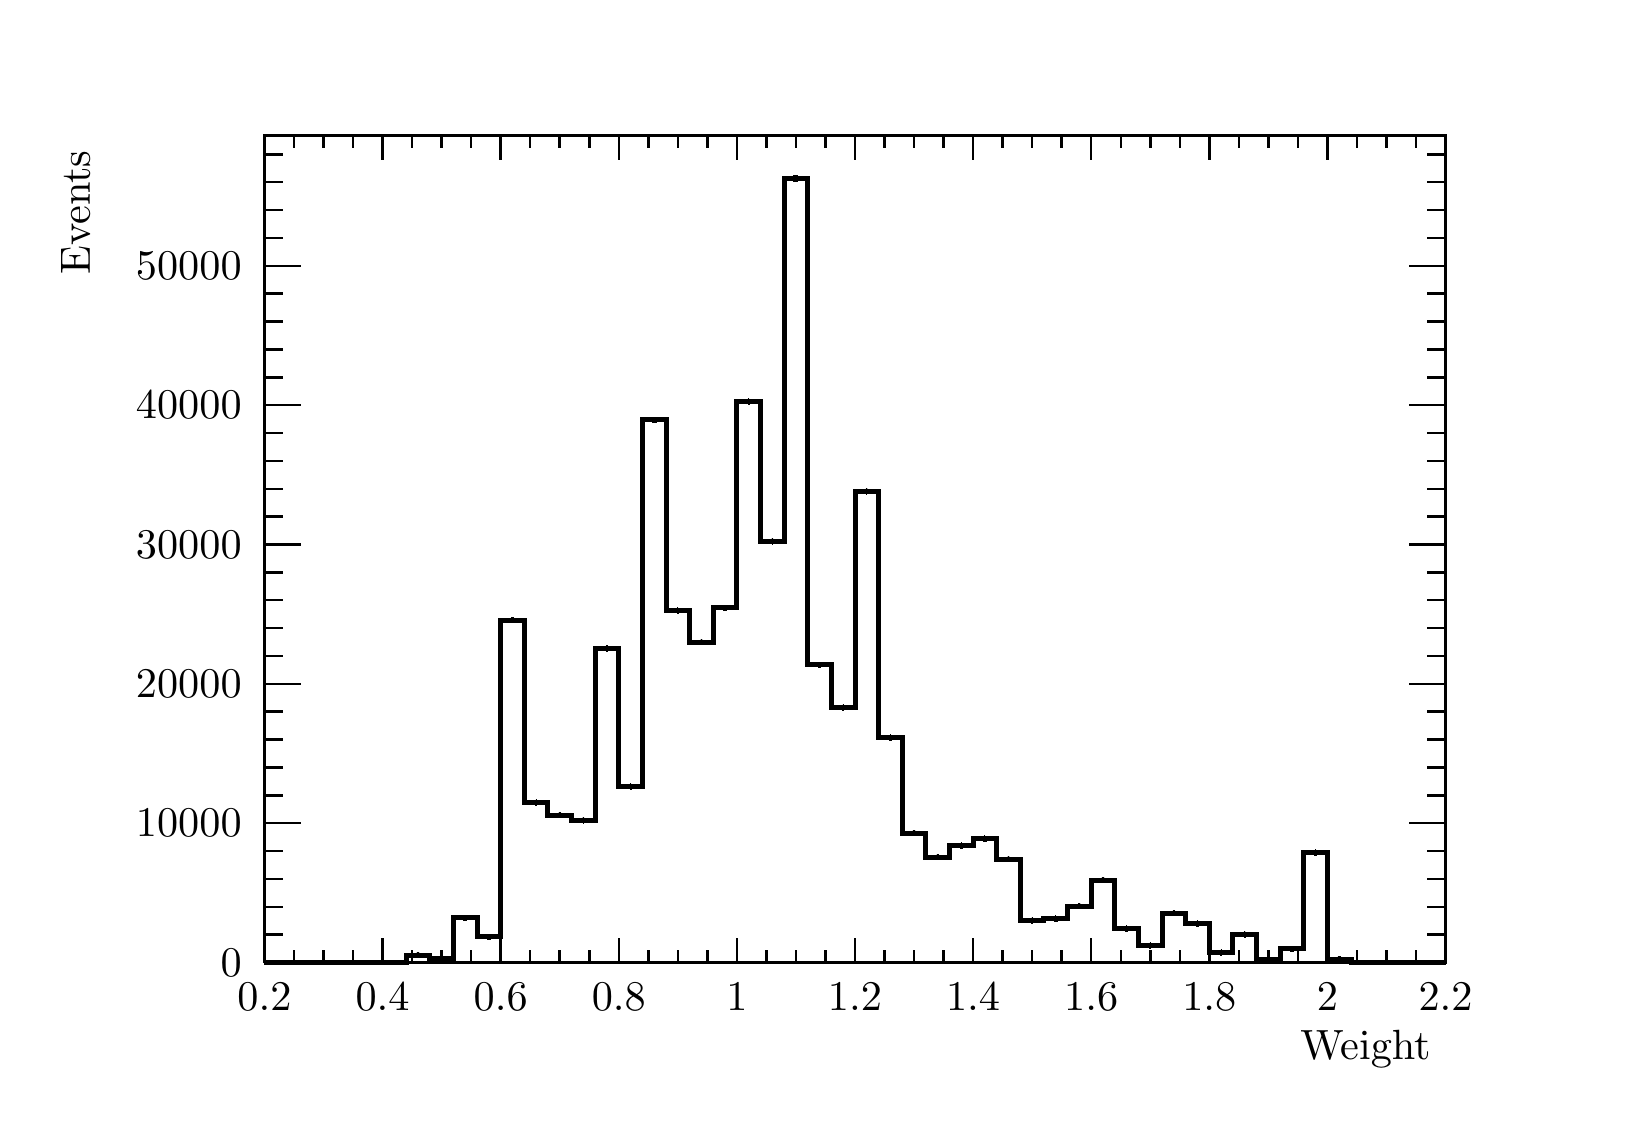
\begin{tikzpicture}
\pgfdeclareplotmark{cross} {
\pgfpathmoveto{\pgfpoint{-0.3\pgfplotmarksize}{\pgfplotmarksize}}
\pgfpathlineto{\pgfpoint{+0.3\pgfplotmarksize}{\pgfplotmarksize}}
\pgfpathlineto{\pgfpoint{+0.3\pgfplotmarksize}{0.3\pgfplotmarksize}}
\pgfpathlineto{\pgfpoint{+1\pgfplotmarksize}{0.3\pgfplotmarksize}}
\pgfpathlineto{\pgfpoint{+1\pgfplotmarksize}{-0.3\pgfplotmarksize}}
\pgfpathlineto{\pgfpoint{+0.3\pgfplotmarksize}{-0.3\pgfplotmarksize}}
\pgfpathlineto{\pgfpoint{+0.3\pgfplotmarksize}{-1.\pgfplotmarksize}}
\pgfpathlineto{\pgfpoint{-0.3\pgfplotmarksize}{-1.\pgfplotmarksize}}
\pgfpathlineto{\pgfpoint{-0.3\pgfplotmarksize}{-0.3\pgfplotmarksize}}
\pgfpathlineto{\pgfpoint{-1.\pgfplotmarksize}{-0.3\pgfplotmarksize}}
\pgfpathlineto{\pgfpoint{-1.\pgfplotmarksize}{0.3\pgfplotmarksize}}
\pgfpathlineto{\pgfpoint{-0.3\pgfplotmarksize}{0.3\pgfplotmarksize}}
\pgfpathclose
\pgfusepathqstroke
}
\pgfdeclareplotmark{cross*} {
\pgfpathmoveto{\pgfpoint{-0.3\pgfplotmarksize}{\pgfplotmarksize}}
\pgfpathlineto{\pgfpoint{+0.3\pgfplotmarksize}{\pgfplotmarksize}}
\pgfpathlineto{\pgfpoint{+0.3\pgfplotmarksize}{0.3\pgfplotmarksize}}
\pgfpathlineto{\pgfpoint{+1\pgfplotmarksize}{0.3\pgfplotmarksize}}
\pgfpathlineto{\pgfpoint{+1\pgfplotmarksize}{-0.3\pgfplotmarksize}}
\pgfpathlineto{\pgfpoint{+0.3\pgfplotmarksize}{-0.3\pgfplotmarksize}}
\pgfpathlineto{\pgfpoint{+0.3\pgfplotmarksize}{-1.\pgfplotmarksize}}
\pgfpathlineto{\pgfpoint{-0.3\pgfplotmarksize}{-1.\pgfplotmarksize}}
\pgfpathlineto{\pgfpoint{-0.3\pgfplotmarksize}{-0.3\pgfplotmarksize}}
\pgfpathlineto{\pgfpoint{-1.\pgfplotmarksize}{-0.3\pgfplotmarksize}}
\pgfpathlineto{\pgfpoint{-1.\pgfplotmarksize}{0.3\pgfplotmarksize}}
\pgfpathlineto{\pgfpoint{-0.3\pgfplotmarksize}{0.3\pgfplotmarksize}}
\pgfpathclose
\pgfusepathqfillstroke
}
\pgfdeclareplotmark{newstar} {
\pgfpathmoveto{\pgfqpoint{0pt}{\pgfplotmarksize}}
\pgfpathlineto{\pgfqpointpolar{44}{0.5\pgfplotmarksize}}
\pgfpathlineto{\pgfqpointpolar{18}{\pgfplotmarksize}}
\pgfpathlineto{\pgfqpointpolar{-20}{0.5\pgfplotmarksize}}
\pgfpathlineto{\pgfqpointpolar{-54}{\pgfplotmarksize}}
\pgfpathlineto{\pgfqpointpolar{-90}{0.5\pgfplotmarksize}}
\pgfpathlineto{\pgfqpointpolar{234}{\pgfplotmarksize}}
\pgfpathlineto{\pgfqpointpolar{198}{0.5\pgfplotmarksize}}
\pgfpathlineto{\pgfqpointpolar{162}{\pgfplotmarksize}}
\pgfpathlineto{\pgfqpointpolar{134}{0.5\pgfplotmarksize}}
\pgfpathclose
\pgfusepathqstroke
}
\pgfdeclareplotmark{newstar*} {
\pgfpathmoveto{\pgfqpoint{0pt}{\pgfplotmarksize}}
\pgfpathlineto{\pgfqpointpolar{44}{0.5\pgfplotmarksize}}
\pgfpathlineto{\pgfqpointpolar{18}{\pgfplotmarksize}}
\pgfpathlineto{\pgfqpointpolar{-20}{0.5\pgfplotmarksize}}
\pgfpathlineto{\pgfqpointpolar{-54}{\pgfplotmarksize}}
\pgfpathlineto{\pgfqpointpolar{-90}{0.5\pgfplotmarksize}}
\pgfpathlineto{\pgfqpointpolar{234}{\pgfplotmarksize}}
\pgfpathlineto{\pgfqpointpolar{198}{0.5\pgfplotmarksize}}
\pgfpathlineto{\pgfqpointpolar{162}{\pgfplotmarksize}}
\pgfpathlineto{\pgfqpointpolar{134}{0.5\pgfplotmarksize}}
\pgfpathclose
\pgfusepathqfillstroke
}
\definecolor{c}{rgb}{1,1,1};
\draw [color=c, fill=c] (0,0) rectangle (20,13.639);
\draw [color=c, fill=c] (3,1.77307) rectangle (18,12.2751);
\definecolor{c}{rgb}{0,0,0};
\draw [c,line width=0.9] (3,1.77307) -- (3,12.2751) -- (18,12.2751) -- (18,1.77307) -- (3,1.77307);
\definecolor{c}{rgb}{1,1,1};
\draw [color=c, fill=c] (3,1.77307) rectangle (18,12.2751);
\definecolor{c}{rgb}{0,0,0};
\draw [c,line width=0.9] (3,1.77307) -- (3,12.2751) -- (18,12.2751) -- (18,1.77307) -- (3,1.77307);
\draw [c,line width=1.8] (4.95,1.86452) -- (4.95,1.86863);
\draw [c,line width=1.8] (4.95,1.86863) -- (4.95,1.87274);
\foreach \P in {(4.95,1.86863)}{\draw[mark options={color=c,fill=c},mark size=2.402402pt, line width=0.000000pt, mark=*,mark size=1pt] plot coordinates {\P};}
\draw [c,line width=1.8] (5.25,1.82567) -- (5.25,1.82881);
\draw [c,line width=1.8] (5.25,1.82881) -- (5.25,1.83195);
\foreach \P in {(5.25,1.82881)}{\draw[mark options={color=c,fill=c},mark size=2.402402pt, line width=0.000000pt, mark=*,mark size=1pt] plot coordinates {\P};}
\draw [c,line width=1.8] (5.55,2.3306) -- (5.55,2.34062);
\draw [c,line width=1.8] (5.55,2.34062) -- (5.55,2.35064);
\foreach \P in {(5.55,2.34062)}{\draw[mark options={color=c,fill=c},mark size=2.402402pt, line width=0.000000pt, mark=*,mark size=1pt] plot coordinates {\P};}
\draw [c,line width=1.8] (5.85,2.09146) -- (5.85,2.09905);
\draw [c,line width=1.8] (5.85,2.09905) -- (5.85,2.10665);
\foreach \P in {(5.85,2.09905)}{\draw[mark options={color=c,fill=c},mark size=2.402402pt, line width=0.000000pt, mark=*,mark size=1pt] plot coordinates {\P};}
\draw [c,line width=1.8] (6.15,6.09393) -- (6.15,6.12167);
\draw [c,line width=1.8] (6.15,6.12167) -- (6.15,6.14942);
\foreach \P in {(6.15,6.12167)}{\draw[mark options={color=c,fill=c},mark size=2.402402pt, line width=0.000000pt, mark=*,mark size=1pt] plot coordinates {\P};}
\draw [c,line width=1.8] (6.45,3.7863) -- (6.45,3.80526);
\draw [c,line width=1.8] (6.45,3.80526) -- (6.45,3.82422);
\foreach \P in {(6.45,3.80526)}{\draw[mark options={color=c,fill=c},mark size=2.402402pt, line width=0.000000pt, mark=*,mark size=1pt] plot coordinates {\P};}
\draw [c,line width=1.8] (6.75,3.62725) -- (6.75,3.64545);
\draw [c,line width=1.8] (6.75,3.64545) -- (6.75,3.66366);
\foreach \P in {(6.75,3.64545)}{\draw[mark options={color=c,fill=c},mark size=2.402402pt, line width=0.000000pt, mark=*,mark size=1pt] plot coordinates {\P};}
\draw [c,line width=1.8] (7.05,3.56227) -- (7.05,3.58015);
\draw [c,line width=1.8] (7.05,3.58015) -- (7.05,3.59803);
\foreach \P in {(7.05,3.58015)}{\draw[mark options={color=c,fill=c},mark size=2.402402pt, line width=0.000000pt, mark=*,mark size=1pt] plot coordinates {\P};}
\draw [c,line width=1.8] (7.35,5.73726) -- (7.35,5.76383);
\draw [c,line width=1.8] (7.35,5.76383) -- (7.35,5.79041);
\foreach \P in {(7.35,5.76383)}{\draw[mark options={color=c,fill=c},mark size=2.402402pt, line width=0.000000pt, mark=*,mark size=1pt] plot coordinates {\P};}
\draw [c,line width=1.8] (7.65,3.98995) -- (7.65,4.00984);
\draw [c,line width=1.8] (7.65,4.00984) -- (7.65,4.02974);
\foreach \P in {(7.65,4.00984)}{\draw[mark options={color=c,fill=c},mark size=2.402402pt, line width=0.000000pt, mark=*,mark size=1pt] plot coordinates {\P};}
\draw [c,line width=1.8] (7.95,8.62916) -- (7.95,8.66408);
\draw [c,line width=1.8] (7.95,8.66408) -- (7.95,8.69901);
\foreach \P in {(7.95,8.66408)}{\draw[mark options={color=c,fill=c},mark size=2.402402pt, line width=0.000000pt, mark=*,mark size=1pt] plot coordinates {\P};}
\draw [c,line width=1.8] (8.25,6.21566) -- (8.25,6.24379);
\draw [c,line width=1.8] (8.25,6.24379) -- (8.25,6.27191);
\foreach \P in {(8.25,6.24379)}{\draw[mark options={color=c,fill=c},mark size=2.402402pt, line width=0.000000pt, mark=*,mark size=1pt] plot coordinates {\P};}
\draw [c,line width=1.8] (8.55,5.81487) -- (8.55,5.8417);
\draw [c,line width=1.8] (8.55,5.8417) -- (8.55,5.86853);
\foreach \P in {(8.55,5.8417)}{\draw[mark options={color=c,fill=c},mark size=2.402402pt, line width=0.000000pt, mark=*,mark size=1pt] plot coordinates {\P};}
\draw [c,line width=1.8] (8.85,6.25024) -- (8.85,6.27847);
\draw [c,line width=1.8] (8.85,6.27847) -- (8.85,6.30671);
\foreach \P in {(8.85,6.27847)}{\draw[mark options={color=c,fill=c},mark size=2.402402pt, line width=0.000000pt, mark=*,mark size=1pt] plot coordinates {\P};}
\draw [c,line width=1.8] (9.15,8.86324) -- (9.15,8.89875);
\draw [c,line width=1.8] (9.15,8.89875) -- (9.15,8.93426);
\foreach \P in {(9.15,8.89875)}{\draw[mark options={color=c,fill=c},mark size=2.402402pt, line width=0.000000pt, mark=*,mark size=1pt] plot coordinates {\P};}
\draw [c,line width=1.8] (9.45,7.0924) -- (9.45,7.12317);
\draw [c,line width=1.8] (9.45,7.12317) -- (9.45,7.15394);
\foreach \P in {(9.45,7.12317)}{\draw[mark options={color=c,fill=c},mark size=2.402402pt, line width=0.000000pt, mark=*,mark size=1pt] plot coordinates {\P};}
\draw [c,line width=1.8] (9.75,11.691) -- (9.75,11.733);
\draw [c,line width=1.8] (9.75,11.733) -- (9.75,11.775);
\foreach \P in {(9.75,11.733)}{\draw[mark options={color=c,fill=c},mark size=2.402402pt, line width=0.000000pt, mark=*,mark size=1pt] plot coordinates {\P};}
\draw [c,line width=1.8] (10.05,5.52843) -- (10.05,5.5543);
\draw [c,line width=1.8] (10.05,5.5543) -- (10.05,5.58016);
\foreach \P in {(10.05,5.5543)}{\draw[mark options={color=c,fill=c},mark size=2.402402pt, line width=0.000000pt, mark=*,mark size=1pt] plot coordinates {\P};}
\draw [c,line width=1.8] (10.35,4.98899) -- (10.35,5.01293);
\draw [c,line width=1.8] (10.35,5.01293) -- (10.35,5.03688);
\foreach \P in {(10.35,5.01293)}{\draw[mark options={color=c,fill=c},mark size=2.402402pt, line width=0.000000pt, mark=*,mark size=1pt] plot coordinates {\P};}
\draw [c,line width=1.8] (10.65,7.72543) -- (10.65,7.75798);
\draw [c,line width=1.8] (10.65,7.75798) -- (10.65,7.79052);
\foreach \P in {(10.65,7.75798)}{\draw[mark options={color=c,fill=c},mark size=2.402402pt, line width=0.000000pt, mark=*,mark size=1pt] plot coordinates {\P};}
\draw [c,line width=1.8] (10.95,4.60642) -- (10.95,4.6289);
\draw [c,line width=1.8] (10.95,4.6289) -- (10.95,4.65138);
\foreach \P in {(10.95,4.6289)}{\draw[mark options={color=c,fill=c},mark size=2.402402pt, line width=0.000000pt, mark=*,mark size=1pt] plot coordinates {\P};}
\draw [c,line width=1.8] (11.25,3.40063) -- (11.25,3.41769);
\draw [c,line width=1.8] (11.25,3.41769) -- (11.25,3.43475);
\foreach \P in {(11.25,3.41769)}{\draw[mark options={color=c,fill=c},mark size=2.402402pt, line width=0.000000pt, mark=*,mark size=1pt] plot coordinates {\P};}
\draw [c,line width=1.8] (11.55,3.09613) -- (11.55,3.11152);
\draw [c,line width=1.8] (11.55,3.11152) -- (11.55,3.12691);
\foreach \P in {(11.55,3.11152)}{\draw[mark options={color=c,fill=c},mark size=2.402402pt, line width=0.000000pt, mark=*,mark size=1pt] plot coordinates {\P};}
\draw [c,line width=1.8] (11.85,3.24184) -- (11.85,3.25806);
\draw [c,line width=1.8] (11.85,3.25806) -- (11.85,3.27427);
\foreach \P in {(11.85,3.25806)}{\draw[mark options={color=c,fill=c},mark size=2.402402pt, line width=0.000000pt, mark=*,mark size=1pt] plot coordinates {\P};}
\draw [c,line width=1.8] (12.15,3.3288) -- (12.15,3.34548);
\draw [c,line width=1.8] (12.15,3.34548) -- (12.15,3.36216);
\foreach \P in {(12.15,3.34548)}{\draw[mark options={color=c,fill=c},mark size=2.402402pt, line width=0.000000pt, mark=*,mark size=1pt] plot coordinates {\P};}
\draw [c,line width=1.8] (12.45,3.07062) -- (12.45,3.08586);
\draw [c,line width=1.8] (12.45,3.08586) -- (12.45,3.1011);
\foreach \P in {(12.45,3.08586)}{\draw[mark options={color=c,fill=c},mark size=2.402402pt, line width=0.000000pt, mark=*,mark size=1pt] plot coordinates {\P};}
\draw [c,line width=1.8] (12.75,2.29868) -- (12.75,2.30841);
\draw [c,line width=1.8] (12.75,2.30841) -- (12.75,2.31815);
\foreach \P in {(12.75,2.30841)}{\draw[mark options={color=c,fill=c},mark size=2.402402pt, line width=0.000000pt, mark=*,mark size=1pt] plot coordinates {\P};}
\draw [c,line width=1.8] (13.05,2.31937) -- (13.05,2.3293);
\draw [c,line width=1.8] (13.05,2.3293) -- (13.05,2.33922);
\foreach \P in {(13.05,2.3293)}{\draw[mark options={color=c,fill=c},mark size=2.402402pt, line width=0.000000pt, mark=*,mark size=1pt] plot coordinates {\P};}
\draw [c,line width=1.8] (13.35,2.47802) -- (13.35,2.48928);
\draw [c,line width=1.8] (13.35,2.48928) -- (13.35,2.50054);
\foreach \P in {(13.35,2.48928)}{\draw[mark options={color=c,fill=c},mark size=2.402402pt, line width=0.000000pt, mark=*,mark size=1pt] plot coordinates {\P};}
\draw [c,line width=1.8] (13.65,2.80731) -- (13.65,2.82093);
\draw [c,line width=1.8] (13.65,2.82093) -- (13.65,2.83455);
\foreach \P in {(13.65,2.82093)}{\draw[mark options={color=c,fill=c},mark size=2.402402pt, line width=0.000000pt, mark=*,mark size=1pt] plot coordinates {\P};}
\draw [c,line width=1.8] (13.95,2.19579) -- (13.95,2.20453);
\draw [c,line width=1.8] (13.95,2.20453) -- (13.95,2.21327);
\foreach \P in {(13.95,2.20453)}{\draw[mark options={color=c,fill=c},mark size=2.402402pt, line width=0.000000pt, mark=*,mark size=1pt] plot coordinates {\P};}
\draw [c,line width=1.8] (14.25,1.98384) -- (14.25,1.99004);
\draw [c,line width=1.8] (14.25,1.99004) -- (14.25,1.99623);
\foreach \P in {(14.25,1.99004)}{\draw[mark options={color=c,fill=c},mark size=2.402402pt, line width=0.000000pt, mark=*,mark size=1pt] plot coordinates {\P};}
\draw [c,line width=1.8] (14.55,2.38973) -- (14.55,2.40026);
\draw [c,line width=1.8] (14.55,2.40026) -- (14.55,2.4108);
\foreach \P in {(14.55,2.40026)}{\draw[mark options={color=c,fill=c},mark size=2.402402pt, line width=0.000000pt, mark=*,mark size=1pt] plot coordinates {\P};}
\draw [c,line width=1.8] (14.85,2.25975) -- (14.85,2.26912);
\draw [c,line width=1.8] (14.85,2.26912) -- (14.85,2.27849);
\foreach \P in {(14.85,2.26912)}{\draw[mark options={color=c,fill=c},mark size=2.402402pt, line width=0.000000pt, mark=*,mark size=1pt] plot coordinates {\P};}
\draw [c,line width=1.8] (15.15,1.89591) -- (15.15,1.90066);
\draw [c,line width=1.8] (15.15,1.90066) -- (15.15,1.90542);
\foreach \P in {(15.15,1.90066)}{\draw[mark options={color=c,fill=c},mark size=2.402402pt, line width=0.000000pt, mark=*,mark size=1pt] plot coordinates {\P};}
\draw [c,line width=1.8] (15.45,2.1233) -- (15.45,2.13126);
\draw [c,line width=1.8] (15.45,2.13126) -- (15.45,2.13922);
\foreach \P in {(15.45,2.13126)}{\draw[mark options={color=c,fill=c},mark size=2.402402pt, line width=0.000000pt, mark=*,mark size=1pt] plot coordinates {\P};}
\draw [c,line width=1.8] (15.75,1.80955) -- (15.75,1.81218);
\draw [c,line width=1.8] (15.75,1.81218) -- (15.75,1.81481);
\foreach \P in {(15.75,1.81218)}{\draw[mark options={color=c,fill=c},mark size=2.402402pt, line width=0.000000pt, mark=*,mark size=1pt] plot coordinates {\P};}
\draw [c,line width=1.8] (16.05,1.94113) -- (16.05,1.94668);
\draw [c,line width=1.8] (16.05,1.94668) -- (16.05,1.95222);
\foreach \P in {(16.05,1.94668)}{\draw[mark options={color=c,fill=c},mark size=2.402402pt, line width=0.000000pt, mark=*,mark size=1pt] plot coordinates {\P};}
\draw [c,line width=1.8] (16.35,3.15385) -- (16.35,3.16957);
\draw [c,line width=1.8] (16.35,3.16957) -- (16.35,3.18529);
\foreach \P in {(16.35,3.16957)}{\draw[mark options={color=c,fill=c},mark size=2.402402pt, line width=0.000000pt, mark=*,mark size=1pt] plot coordinates {\P};}
\draw [c,line width=1.8] (16.65,1.81537) -- (16.65,1.81819);
\draw [c,line width=1.8] (16.65,1.81819) -- (16.65,1.82102);
\foreach \P in {(16.65,1.81819)}{\draw[mark options={color=c,fill=c},mark size=2.402402pt, line width=0.000000pt, mark=*,mark size=1pt] plot coordinates {\P};}
\draw [c,line width=1.8] (3,1.77307) -- (3.3,1.77307) -- (3.3,1.77307) -- (3.6,1.77307) -- (3.6,1.77307) -- (3.9,1.77307) -- (3.9,1.77307) -- (4.2,1.77307) -- (4.2,1.77307) -- (4.5,1.77307) -- (4.5,1.77307) -- (4.8,1.77307) -- (4.8,1.86863) --
 (5.1,1.86863) -- (5.1,1.82881) -- (5.4,1.82881) -- (5.4,2.34062) -- (5.7,2.34062) -- (5.7,2.09905) -- (6,2.09905) -- (6,6.12167) -- (6.3,6.12167) -- (6.3,3.80526) -- (6.6,3.80526) -- (6.6,3.64545) -- (6.9,3.64545) -- (6.9,3.58015) -- (7.2,3.58015)
 -- (7.2,5.76383) -- (7.5,5.76383) -- (7.5,4.00984) -- (7.8,4.00984) -- (7.8,8.66408) -- (8.1,8.66408) -- (8.1,6.24379) -- (8.4,6.24379) -- (8.4,5.8417) -- (8.7,5.8417) -- (8.7,6.27847) -- (9,6.27847) -- (9,8.89875) -- (9.3,8.89875) -- (9.3,7.12317)
 -- (9.6,7.12317) -- (9.6,11.733) -- (9.9,11.733) -- (9.9,5.5543) -- (10.2,5.5543) -- (10.2,5.01293) -- (10.5,5.01293) -- (10.5,7.75798) -- (10.8,7.75798) -- (10.8,4.6289) -- (11.1,4.6289) -- (11.1,3.41769) -- (11.4,3.41769) -- (11.4,3.11152) --
 (11.7,3.11152) -- (11.7,3.25806) -- (12,3.25806) -- (12,3.34548) -- (12.3,3.34548) -- (12.3,3.08586) -- (12.6,3.08586) -- (12.6,2.30841) -- (12.9,2.30841) -- (12.9,2.3293) -- (13.2,2.3293) -- (13.2,2.48928) -- (13.5,2.48928) -- (13.5,2.82093) --
 (13.8,2.82093) -- (13.8,2.20453) -- (14.1,2.20453) -- (14.1,1.99004) -- (14.4,1.99004) -- (14.4,2.40026) -- (14.7,2.40026) -- (14.7,2.26912) -- (15,2.26912) -- (15,1.90066) -- (15.3,1.90066) -- (15.3,2.13126) -- (15.6,2.13126) -- (15.6,1.81218) --
 (15.9,1.81218) -- (15.9,1.94668) -- (16.2,1.94668) -- (16.2,3.16957) -- (16.5,3.16957) -- (16.5,1.81819) -- (16.8,1.81819) -- (16.8,1.77307) -- (17.1,1.77307) -- (17.1,1.77307) -- (17.4,1.77307) -- (17.4,1.77307) -- (17.7,1.77307) -- (17.7,1.77307)
 -- (18,1.77307);
\draw [c,line width=0.9] (3,1.77307) -- (18,1.77307);
\draw [c,line width=0.9] (3,2.07994) -- (3,1.77307);
\draw [c,line width=0.9] (3.375,1.9265) -- (3.375,1.77307);
\draw [c,line width=0.9] (3.75,1.9265) -- (3.75,1.77307);
\draw [c,line width=0.9] (4.125,1.9265) -- (4.125,1.77307);
\draw [c,line width=0.9] (4.5,2.07994) -- (4.5,1.77307);
\draw [c,line width=0.9] (4.875,1.9265) -- (4.875,1.77307);
\draw [c,line width=0.9] (5.25,1.9265) -- (5.25,1.77307);
\draw [c,line width=0.9] (5.625,1.9265) -- (5.625,1.77307);
\draw [c,line width=0.9] (6,2.07994) -- (6,1.77307);
\draw [c,line width=0.9] (6.375,1.9265) -- (6.375,1.77307);
\draw [c,line width=0.9] (6.75,1.9265) -- (6.75,1.77307);
\draw [c,line width=0.9] (7.125,1.9265) -- (7.125,1.77307);
\draw [c,line width=0.9] (7.5,2.07994) -- (7.5,1.77307);
\draw [c,line width=0.9] (7.875,1.9265) -- (7.875,1.77307);
\draw [c,line width=0.9] (8.25,1.9265) -- (8.25,1.77307);
\draw [c,line width=0.9] (8.625,1.9265) -- (8.625,1.77307);
\draw [c,line width=0.9] (9,2.07994) -- (9,1.77307);
\draw [c,line width=0.9] (9.375,1.9265) -- (9.375,1.77307);
\draw [c,line width=0.9] (9.75,1.9265) -- (9.75,1.77307);
\draw [c,line width=0.9] (10.125,1.9265) -- (10.125,1.77307);
\draw [c,line width=0.9] (10.5,2.07994) -- (10.5,1.77307);
\draw [c,line width=0.9] (10.875,1.9265) -- (10.875,1.77307);
\draw [c,line width=0.9] (11.25,1.9265) -- (11.25,1.77307);
\draw [c,line width=0.9] (11.625,1.9265) -- (11.625,1.77307);
\draw [c,line width=0.9] (12,2.07994) -- (12,1.77307);
\draw [c,line width=0.9] (12.375,1.9265) -- (12.375,1.77307);
\draw [c,line width=0.9] (12.75,1.9265) -- (12.75,1.77307);
\draw [c,line width=0.9] (13.125,1.9265) -- (13.125,1.77307);
\draw [c,line width=0.9] (13.5,2.07994) -- (13.5,1.77307);
\draw [c,line width=0.9] (13.875,1.9265) -- (13.875,1.77307);
\draw [c,line width=0.9] (14.25,1.9265) -- (14.25,1.77307);
\draw [c,line width=0.9] (14.625,1.9265) -- (14.625,1.77307);
\draw [c,line width=0.9] (15,2.07994) -- (15,1.77307);
\draw [c,line width=0.9] (15.375,1.9265) -- (15.375,1.77307);
\draw [c,line width=0.9] (15.75,1.9265) -- (15.75,1.77307);
\draw [c,line width=0.9] (16.125,1.9265) -- (16.125,1.77307);
\draw [c,line width=0.9] (16.5,2.07994) -- (16.5,1.77307);
\draw [c,line width=0.9] (16.875,1.9265) -- (16.875,1.77307);
\draw [c,line width=0.9] (17.25,1.9265) -- (17.25,1.77307);
\draw [c,line width=0.9] (17.625,1.9265) -- (17.625,1.77307);
\draw [c,line width=0.9] (18,2.07994) -- (18,1.77307);
\draw [anchor=base] (3,1.15931) node[scale=1.52731, color=c, rotate=0]{0.2};
\draw [anchor=base] (4.5,1.15931) node[scale=1.52731, color=c, rotate=0]{0.4};
\draw [anchor=base] (6,1.15931) node[scale=1.52731, color=c, rotate=0]{0.6};
\draw [anchor=base] (7.5,1.15931) node[scale=1.52731, color=c, rotate=0]{0.8};
\draw [anchor=base] (9,1.15931) node[scale=1.52731, color=c, rotate=0]{1};
\draw [anchor=base] (10.5,1.15931) node[scale=1.52731, color=c, rotate=0]{1.2};
\draw [anchor=base] (12,1.15931) node[scale=1.52731, color=c, rotate=0]{1.4};
\draw [anchor=base] (13.5,1.15931) node[scale=1.52731, color=c, rotate=0]{1.6};
\draw [anchor=base] (15,1.15931) node[scale=1.52731, color=c, rotate=0]{1.8};
\draw [anchor=base] (16.5,1.15931) node[scale=1.52731, color=c, rotate=0]{2};
\draw [anchor=base] (18,1.15931) node[scale=1.52731, color=c, rotate=0]{2.2};
\draw [anchor= east] (18,0.681948) node[scale=1.52731, color=c, rotate=0]{ Weight};
\draw [c,line width=0.9] (3,12.2751) -- (18,12.2751);
\draw [c,line width=0.9] (3,11.9682) -- (3,12.2751);
\draw [c,line width=0.9] (3.375,12.1216) -- (3.375,12.2751);
\draw [c,line width=0.9] (3.75,12.1216) -- (3.75,12.2751);
\draw [c,line width=0.9] (4.125,12.1216) -- (4.125,12.2751);
\draw [c,line width=0.9] (4.5,11.9682) -- (4.5,12.2751);
\draw [c,line width=0.9] (4.875,12.1216) -- (4.875,12.2751);
\draw [c,line width=0.9] (5.25,12.1216) -- (5.25,12.2751);
\draw [c,line width=0.9] (5.625,12.1216) -- (5.625,12.2751);
\draw [c,line width=0.9] (6,11.9682) -- (6,12.2751);
\draw [c,line width=0.9] (6.375,12.1216) -- (6.375,12.2751);
\draw [c,line width=0.9] (6.75,12.1216) -- (6.75,12.2751);
\draw [c,line width=0.9] (7.125,12.1216) -- (7.125,12.2751);
\draw [c,line width=0.9] (7.5,11.9682) -- (7.5,12.2751);
\draw [c,line width=0.9] (7.875,12.1216) -- (7.875,12.2751);
\draw [c,line width=0.9] (8.25,12.1216) -- (8.25,12.2751);
\draw [c,line width=0.9] (8.625,12.1216) -- (8.625,12.2751);
\draw [c,line width=0.9] (9,11.9682) -- (9,12.2751);
\draw [c,line width=0.9] (9.375,12.1216) -- (9.375,12.2751);
\draw [c,line width=0.9] (9.75,12.1216) -- (9.75,12.2751);
\draw [c,line width=0.9] (10.125,12.1216) -- (10.125,12.2751);
\draw [c,line width=0.9] (10.5,11.9682) -- (10.5,12.2751);
\draw [c,line width=0.9] (10.875,12.1216) -- (10.875,12.2751);
\draw [c,line width=0.9] (11.25,12.1216) -- (11.25,12.2751);
\draw [c,line width=0.9] (11.625,12.1216) -- (11.625,12.2751);
\draw [c,line width=0.9] (12,11.9682) -- (12,12.2751);
\draw [c,line width=0.9] (12.375,12.1216) -- (12.375,12.2751);
\draw [c,line width=0.9] (12.75,12.1216) -- (12.75,12.2751);
\draw [c,line width=0.9] (13.125,12.1216) -- (13.125,12.2751);
\draw [c,line width=0.9] (13.5,11.9682) -- (13.5,12.2751);
\draw [c,line width=0.9] (13.875,12.1216) -- (13.875,12.2751);
\draw [c,line width=0.9] (14.25,12.1216) -- (14.25,12.2751);
\draw [c,line width=0.9] (14.625,12.1216) -- (14.625,12.2751);
\draw [c,line width=0.9] (15,11.9682) -- (15,12.2751);
\draw [c,line width=0.9] (15.375,12.1216) -- (15.375,12.2751);
\draw [c,line width=0.9] (15.75,12.1216) -- (15.75,12.2751);
\draw [c,line width=0.9] (16.125,12.1216) -- (16.125,12.2751);
\draw [c,line width=0.9] (16.5,11.9682) -- (16.5,12.2751);
\draw [c,line width=0.9] (16.875,12.1216) -- (16.875,12.2751);
\draw [c,line width=0.9] (17.25,12.1216) -- (17.25,12.2751);
\draw [c,line width=0.9] (17.625,12.1216) -- (17.625,12.2751);
\draw [c,line width=0.9] (18,11.9682) -- (18,12.2751);
\draw [c,line width=0.9] (3,1.77307) -- (3,12.2751);
\draw [c,line width=0.9] (3.462,1.77307) -- (3,1.77307);
\draw [c,line width=0.9] (3.231,2.12701) -- (3,2.12701);
\draw [c,line width=0.9] (3.231,2.48096) -- (3,2.48096);
\draw [c,line width=0.9] (3.231,2.83491) -- (3,2.83491);
\draw [c,line width=0.9] (3.231,3.18886) -- (3,3.18886);
\draw [c,line width=0.9] (3.462,3.54281) -- (3,3.54281);
\draw [c,line width=0.9] (3.231,3.89676) -- (3,3.89676);
\draw [c,line width=0.9] (3.231,4.2507) -- (3,4.2507);
\draw [c,line width=0.9] (3.231,4.60465) -- (3,4.60465);
\draw [c,line width=0.9] (3.231,4.9586) -- (3,4.9586);
\draw [c,line width=0.9] (3.462,5.31255) -- (3,5.31255);
\draw [c,line width=0.9] (3.231,5.6665) -- (3,5.6665);
\draw [c,line width=0.9] (3.231,6.02044) -- (3,6.02044);
\draw [c,line width=0.9] (3.231,6.37439) -- (3,6.37439);
\draw [c,line width=0.9] (3.231,6.72834) -- (3,6.72834);
\draw [c,line width=0.9] (3.462,7.08229) -- (3,7.08229);
\draw [c,line width=0.9] (3.231,7.43624) -- (3,7.43624);
\draw [c,line width=0.9] (3.231,7.79019) -- (3,7.79019);
\draw [c,line width=0.9] (3.231,8.14413) -- (3,8.14413);
\draw [c,line width=0.9] (3.231,8.49808) -- (3,8.49808);
\draw [c,line width=0.9] (3.462,8.85203) -- (3,8.85203);
\draw [c,line width=0.9] (3.231,9.20598) -- (3,9.20598);
\draw [c,line width=0.9] (3.231,9.55993) -- (3,9.55993);
\draw [c,line width=0.9] (3.231,9.91388) -- (3,9.91388);
\draw [c,line width=0.9] (3.231,10.2678) -- (3,10.2678);
\draw [c,line width=0.9] (3.462,10.6218) -- (3,10.6218);
\draw [c,line width=0.9] (3.462,10.6218) -- (3,10.6218);
\draw [c,line width=0.9] (3.231,10.9757) -- (3,10.9757);
\draw [c,line width=0.9] (3.231,11.3297) -- (3,11.3297);
\draw [c,line width=0.9] (3.231,11.6836) -- (3,11.6836);
\draw [c,line width=0.9] (3.231,12.0376) -- (3,12.0376);
\draw [anchor= east] (2.9,1.77307) node[scale=1.52731, color=c, rotate=0]{0};
\draw [anchor= east] (2.9,3.54281) node[scale=1.52731, color=c, rotate=0]{10000};
\draw [anchor= east] (2.9,5.31255) node[scale=1.52731, color=c, rotate=0]{20000};
\draw [anchor= east] (2.9,7.08229) node[scale=1.52731, color=c, rotate=0]{30000};
\draw [anchor= east] (2.9,8.85203) node[scale=1.52731, color=c, rotate=0]{40000};
\draw [anchor= east] (2.9,10.6218) node[scale=1.52731, color=c, rotate=0]{50000};
\draw [anchor= east] (0.6,12.2751) node[scale=1.52731, color=c, rotate=90]{ Events};
\draw [c,line width=0.9] (18,1.77307) -- (18,12.2751);
\draw [c,line width=0.9] (17.538,1.77307) -- (18,1.77307);
\draw [c,line width=0.9] (17.769,2.12701) -- (18,2.12701);
\draw [c,line width=0.9] (17.769,2.48096) -- (18,2.48096);
\draw [c,line width=0.9] (17.769,2.83491) -- (18,2.83491);
\draw [c,line width=0.9] (17.769,3.18886) -- (18,3.18886);
\draw [c,line width=0.9] (17.538,3.54281) -- (18,3.54281);
\draw [c,line width=0.9] (17.769,3.89676) -- (18,3.89676);
\draw [c,line width=0.9] (17.769,4.2507) -- (18,4.2507);
\draw [c,line width=0.9] (17.769,4.60465) -- (18,4.60465);
\draw [c,line width=0.9] (17.769,4.9586) -- (18,4.9586);
\draw [c,line width=0.9] (17.538,5.31255) -- (18,5.31255);
\draw [c,line width=0.9] (17.769,5.6665) -- (18,5.6665);
\draw [c,line width=0.9] (17.769,6.02044) -- (18,6.02044);
\draw [c,line width=0.9] (17.769,6.37439) -- (18,6.37439);
\draw [c,line width=0.9] (17.769,6.72834) -- (18,6.72834);
\draw [c,line width=0.9] (17.538,7.08229) -- (18,7.08229);
\draw [c,line width=0.9] (17.769,7.43624) -- (18,7.43624);
\draw [c,line width=0.9] (17.769,7.79019) -- (18,7.79019);
\draw [c,line width=0.9] (17.769,8.14413) -- (18,8.14413);
\draw [c,line width=0.9] (17.769,8.49808) -- (18,8.49808);
\draw [c,line width=0.9] (17.538,8.85203) -- (18,8.85203);
\draw [c,line width=0.9] (17.769,9.20598) -- (18,9.20598);
\draw [c,line width=0.9] (17.769,9.55993) -- (18,9.55993);
\draw [c,line width=0.9] (17.769,9.91388) -- (18,9.91388);
\draw [c,line width=0.9] (17.769,10.2678) -- (18,10.2678);
\draw [c,line width=0.9] (17.538,10.6218) -- (18,10.6218);
\draw [c,line width=0.9] (17.538,10.6218) -- (18,10.6218);
\draw [c,line width=0.9] (17.769,10.9757) -- (18,10.9757);
\draw [c,line width=0.9] (17.769,11.3297) -- (18,11.3297);
\draw [c,line width=0.9] (17.769,11.6836) -- (18,11.6836);
\draw [c,line width=0.9] (17.769,12.0376) -- (18,12.0376);
\definecolor{c}{rgb}{1,1,1};
\draw [color=c, fill=c] (2,12.8206) rectangle (18,13.5708);
\definecolor{c}{rgb}{0,0,0};
%\draw (10,13.1957) node[scale=1.40004, color=c, rotate=0]{FHC: nueswap};
\end{tikzpicture}

		\end{adjustbox}
		\caption{FHC: reco \nue}
	\end{subfigure}	\\
	\begin{subfigure}[t]{.5\linewidth}
		\begin{adjustbox}{max totalsize=\linewidth, center}
			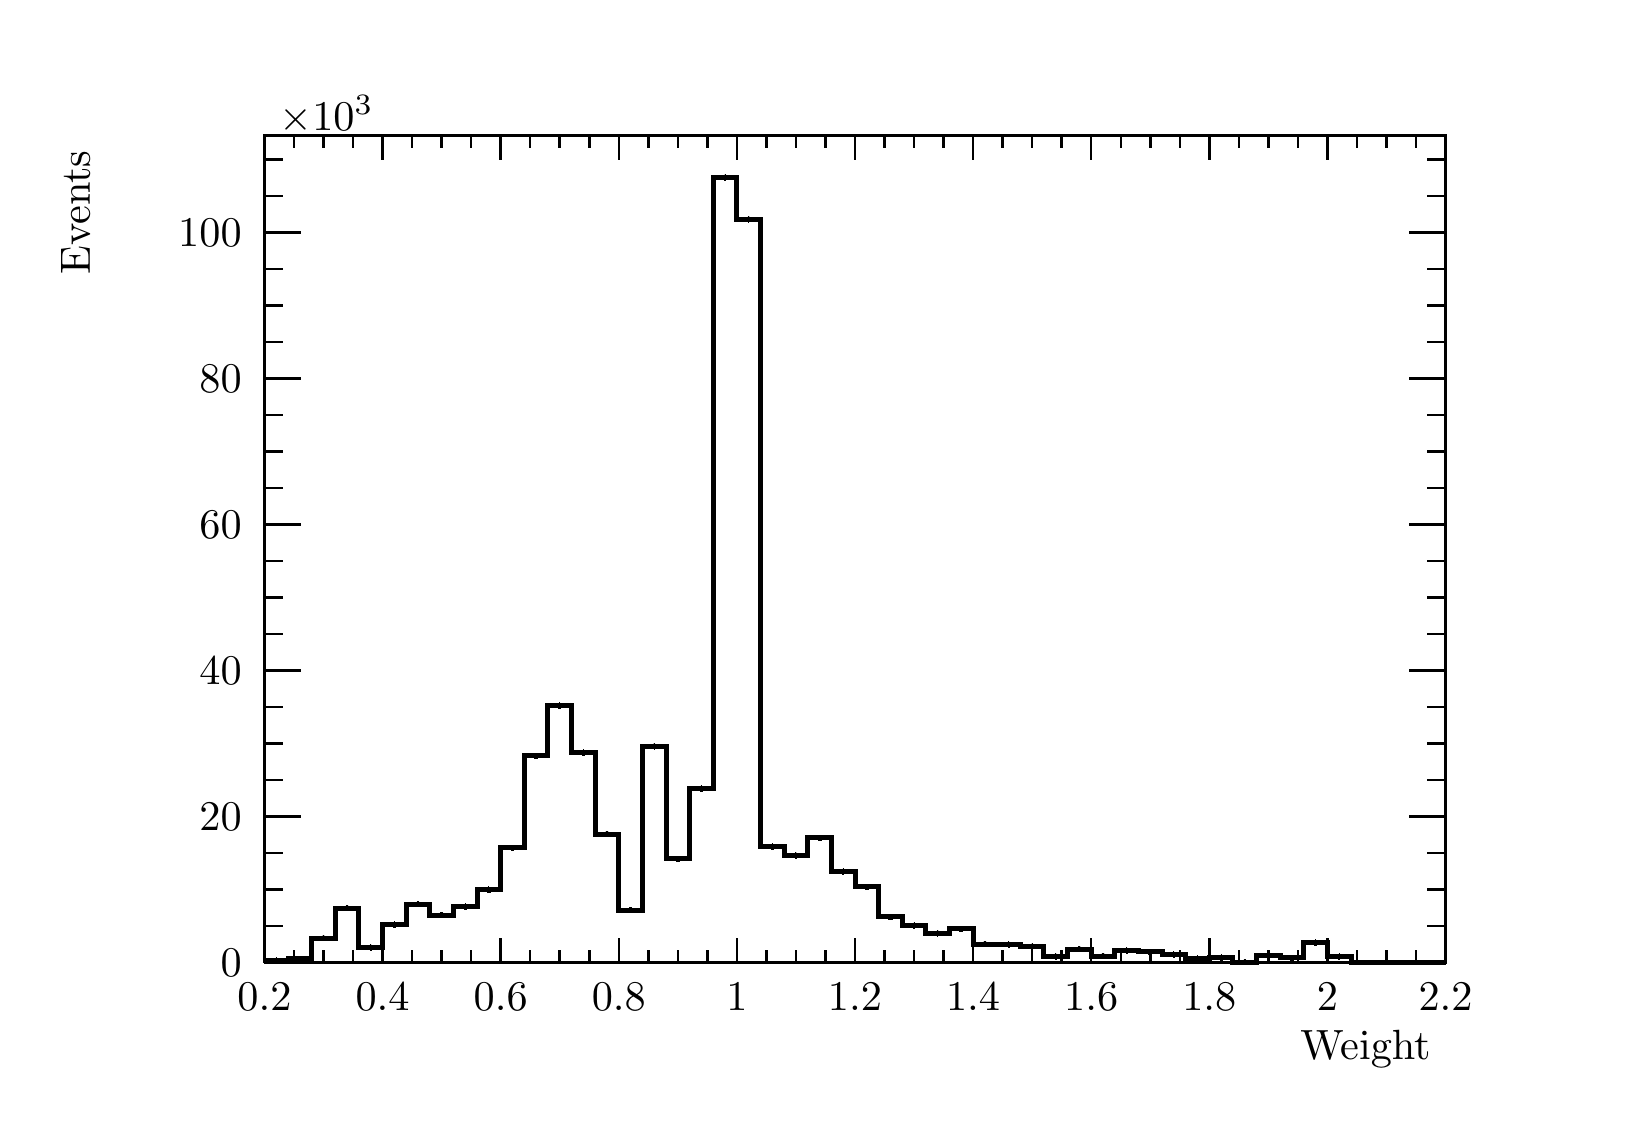
\begin{tikzpicture}
\pgfdeclareplotmark{cross} {
\pgfpathmoveto{\pgfpoint{-0.3\pgfplotmarksize}{\pgfplotmarksize}}
\pgfpathlineto{\pgfpoint{+0.3\pgfplotmarksize}{\pgfplotmarksize}}
\pgfpathlineto{\pgfpoint{+0.3\pgfplotmarksize}{0.3\pgfplotmarksize}}
\pgfpathlineto{\pgfpoint{+1\pgfplotmarksize}{0.3\pgfplotmarksize}}
\pgfpathlineto{\pgfpoint{+1\pgfplotmarksize}{-0.3\pgfplotmarksize}}
\pgfpathlineto{\pgfpoint{+0.3\pgfplotmarksize}{-0.3\pgfplotmarksize}}
\pgfpathlineto{\pgfpoint{+0.3\pgfplotmarksize}{-1.\pgfplotmarksize}}
\pgfpathlineto{\pgfpoint{-0.3\pgfplotmarksize}{-1.\pgfplotmarksize}}
\pgfpathlineto{\pgfpoint{-0.3\pgfplotmarksize}{-0.3\pgfplotmarksize}}
\pgfpathlineto{\pgfpoint{-1.\pgfplotmarksize}{-0.3\pgfplotmarksize}}
\pgfpathlineto{\pgfpoint{-1.\pgfplotmarksize}{0.3\pgfplotmarksize}}
\pgfpathlineto{\pgfpoint{-0.3\pgfplotmarksize}{0.3\pgfplotmarksize}}
\pgfpathclose
\pgfusepathqstroke
}
\pgfdeclareplotmark{cross*} {
\pgfpathmoveto{\pgfpoint{-0.3\pgfplotmarksize}{\pgfplotmarksize}}
\pgfpathlineto{\pgfpoint{+0.3\pgfplotmarksize}{\pgfplotmarksize}}
\pgfpathlineto{\pgfpoint{+0.3\pgfplotmarksize}{0.3\pgfplotmarksize}}
\pgfpathlineto{\pgfpoint{+1\pgfplotmarksize}{0.3\pgfplotmarksize}}
\pgfpathlineto{\pgfpoint{+1\pgfplotmarksize}{-0.3\pgfplotmarksize}}
\pgfpathlineto{\pgfpoint{+0.3\pgfplotmarksize}{-0.3\pgfplotmarksize}}
\pgfpathlineto{\pgfpoint{+0.3\pgfplotmarksize}{-1.\pgfplotmarksize}}
\pgfpathlineto{\pgfpoint{-0.3\pgfplotmarksize}{-1.\pgfplotmarksize}}
\pgfpathlineto{\pgfpoint{-0.3\pgfplotmarksize}{-0.3\pgfplotmarksize}}
\pgfpathlineto{\pgfpoint{-1.\pgfplotmarksize}{-0.3\pgfplotmarksize}}
\pgfpathlineto{\pgfpoint{-1.\pgfplotmarksize}{0.3\pgfplotmarksize}}
\pgfpathlineto{\pgfpoint{-0.3\pgfplotmarksize}{0.3\pgfplotmarksize}}
\pgfpathclose
\pgfusepathqfillstroke
}
\pgfdeclareplotmark{newstar} {
\pgfpathmoveto{\pgfqpoint{0pt}{\pgfplotmarksize}}
\pgfpathlineto{\pgfqpointpolar{44}{0.5\pgfplotmarksize}}
\pgfpathlineto{\pgfqpointpolar{18}{\pgfplotmarksize}}
\pgfpathlineto{\pgfqpointpolar{-20}{0.5\pgfplotmarksize}}
\pgfpathlineto{\pgfqpointpolar{-54}{\pgfplotmarksize}}
\pgfpathlineto{\pgfqpointpolar{-90}{0.5\pgfplotmarksize}}
\pgfpathlineto{\pgfqpointpolar{234}{\pgfplotmarksize}}
\pgfpathlineto{\pgfqpointpolar{198}{0.5\pgfplotmarksize}}
\pgfpathlineto{\pgfqpointpolar{162}{\pgfplotmarksize}}
\pgfpathlineto{\pgfqpointpolar{134}{0.5\pgfplotmarksize}}
\pgfpathclose
\pgfusepathqstroke
}
\pgfdeclareplotmark{newstar*} {
\pgfpathmoveto{\pgfqpoint{0pt}{\pgfplotmarksize}}
\pgfpathlineto{\pgfqpointpolar{44}{0.5\pgfplotmarksize}}
\pgfpathlineto{\pgfqpointpolar{18}{\pgfplotmarksize}}
\pgfpathlineto{\pgfqpointpolar{-20}{0.5\pgfplotmarksize}}
\pgfpathlineto{\pgfqpointpolar{-54}{\pgfplotmarksize}}
\pgfpathlineto{\pgfqpointpolar{-90}{0.5\pgfplotmarksize}}
\pgfpathlineto{\pgfqpointpolar{234}{\pgfplotmarksize}}
\pgfpathlineto{\pgfqpointpolar{198}{0.5\pgfplotmarksize}}
\pgfpathlineto{\pgfqpointpolar{162}{\pgfplotmarksize}}
\pgfpathlineto{\pgfqpointpolar{134}{0.5\pgfplotmarksize}}
\pgfpathclose
\pgfusepathqfillstroke
}
\definecolor{c}{rgb}{1,1,1};
\draw [color=c, fill=c] (0,0) rectangle (20,13.639);
\draw [color=c, fill=c] (3,1.77307) rectangle (18,12.2751);
\definecolor{c}{rgb}{0,0,0};
\draw [c,line width=0.9] (3,1.77307) -- (3,12.2751) -- (18,12.2751) -- (18,1.77307) -- (3,1.77307);
\definecolor{c}{rgb}{1,1,1};
\draw [color=c, fill=c] (3,1.77307) rectangle (18,12.2751);
\definecolor{c}{rgb}{0,0,0};
\draw [c,line width=0.9] (3,1.77307) -- (3,12.2751) -- (18,12.2751) -- (18,1.77307) -- (3,1.77307);
\draw [c,line width=1.8] (3.15,1.79585) -- (3.15,1.79735);
\draw [c,line width=1.8] (3.15,1.79735) -- (3.15,1.79885);
\foreach \P in {(3.15,1.79735)}{\draw[mark options={color=c,fill=c},mark size=2.402402pt, line width=0.000000pt, mark=*,mark size=1pt] plot coordinates {\P};}
\draw [c,line width=1.8] (3.45,1.81889) -- (3.45,1.82099);
\draw [c,line width=1.8] (3.45,1.82099) -- (3.45,1.8231);
\foreach \P in {(3.45,1.82099)}{\draw[mark options={color=c,fill=c},mark size=2.402402pt, line width=0.000000pt, mark=*,mark size=1pt] plot coordinates {\P};}
\draw [c,line width=1.8] (3.75,2.07706) -- (3.75,2.08241);
\draw [c,line width=1.8] (3.75,2.08241) -- (3.75,2.08777);
\foreach \P in {(3.75,2.08241)}{\draw[mark options={color=c,fill=c},mark size=2.402402pt, line width=0.000000pt, mark=*,mark size=1pt] plot coordinates {\P};}
\draw [c,line width=1.8] (4.05,2.45662) -- (4.05,2.46462);
\draw [c,line width=1.8] (4.05,2.46462) -- (4.05,2.47263);
\foreach \P in {(4.05,2.46462)}{\draw[mark options={color=c,fill=c},mark size=2.402402pt, line width=0.000000pt, mark=*,mark size=1pt] plot coordinates {\P};}
\draw [c,line width=1.8] (4.35,1.96148) -- (4.35,1.9657);
\draw [c,line width=1.8] (4.35,1.9657) -- (4.35,1.96993);
\foreach \P in {(4.35,1.9657)}{\draw[mark options={color=c,fill=c},mark size=2.402402pt, line width=0.000000pt, mark=*,mark size=1pt] plot coordinates {\P};}
\draw [c,line width=1.8] (4.65,2.24751) -- (4.65,2.25419);
\draw [c,line width=1.8] (4.65,2.25419) -- (4.65,2.26087);
\foreach \P in {(4.65,2.25419)}{\draw[mark options={color=c,fill=c},mark size=2.402402pt, line width=0.000000pt, mark=*,mark size=1pt] plot coordinates {\P};}
\draw [c,line width=1.8] (4.95,2.50602) -- (4.95,2.51431);
\draw [c,line width=1.8] (4.95,2.51431) -- (4.95,2.5226);
\foreach \P in {(4.95,2.51431)}{\draw[mark options={color=c,fill=c},mark size=2.402402pt, line width=0.000000pt, mark=*,mark size=1pt] plot coordinates {\P};}
\draw [c,line width=1.8] (5.25,2.3688) -- (5.25,2.37628);
\draw [c,line width=1.8] (5.25,2.37628) -- (5.25,2.38376);
\foreach \P in {(5.25,2.37628)}{\draw[mark options={color=c,fill=c},mark size=2.402402pt, line width=0.000000pt, mark=*,mark size=1pt] plot coordinates {\P};}
\draw [c,line width=1.8] (5.55,2.47422) -- (5.55,2.48233);
\draw [c,line width=1.8] (5.55,2.48233) -- (5.55,2.49044);
\foreach \P in {(5.55,2.48233)}{\draw[mark options={color=c,fill=c},mark size=2.402402pt, line width=0.000000pt, mark=*,mark size=1pt] plot coordinates {\P};}
\draw [c,line width=1.8] (5.85,2.6887) -- (5.85,2.69796);
\draw [c,line width=1.8] (5.85,2.69796) -- (5.85,2.70721);
\foreach \P in {(5.85,2.69796)}{\draw[mark options={color=c,fill=c},mark size=2.402402pt, line width=0.000000pt, mark=*,mark size=1pt] plot coordinates {\P};}
\draw [c,line width=1.8] (6.15,3.21891) -- (6.15,3.23053);
\draw [c,line width=1.8] (6.15,3.23053) -- (6.15,3.24215);
\foreach \P in {(6.15,3.23053)}{\draw[mark options={color=c,fill=c},mark size=2.402402pt, line width=0.000000pt, mark=*,mark size=1pt] plot coordinates {\P};}
\draw [c,line width=1.8] (6.45,4.38214) -- (6.45,4.39774);
\draw [c,line width=1.8] (6.45,4.39774) -- (6.45,4.41334);
\foreach \P in {(6.45,4.39774)}{\draw[mark options={color=c,fill=c},mark size=2.402402pt, line width=0.000000pt, mark=*,mark size=1pt] plot coordinates {\P};}
\draw [c,line width=1.8] (6.75,5.01851) -- (6.75,5.0359);
\draw [c,line width=1.8] (6.75,5.0359) -- (6.75,5.0533);
\foreach \P in {(6.75,5.0359)}{\draw[mark options={color=c,fill=c},mark size=2.402402pt, line width=0.000000pt, mark=*,mark size=1pt] plot coordinates {\P};}
\draw [c,line width=1.8] (7.05,4.42281) -- (7.05,4.43853);
\draw [c,line width=1.8] (7.05,4.43853) -- (7.05,4.45425);
\foreach \P in {(7.05,4.43853)}{\draw[mark options={color=c,fill=c},mark size=2.402402pt, line width=0.000000pt, mark=*,mark size=1pt] plot coordinates {\P};}
\draw [c,line width=1.8] (7.35,3.39316) -- (7.35,3.40546);
\draw [c,line width=1.8] (7.35,3.40546) -- (7.35,3.41776);
\foreach \P in {(7.35,3.40546)}{\draw[mark options={color=c,fill=c},mark size=2.402402pt, line width=0.000000pt, mark=*,mark size=1pt] plot coordinates {\P};}
\draw [c,line width=1.8] (7.65,2.43137) -- (7.65,2.43922);
\draw [c,line width=1.8] (7.65,2.43922) -- (7.65,2.44708);
\foreach \P in {(7.65,2.43922)}{\draw[mark options={color=c,fill=c},mark size=2.402402pt, line width=0.000000pt, mark=*,mark size=1pt] plot coordinates {\P};}
\draw [c,line width=1.8] (7.95,4.50378) -- (7.95,4.51974);
\draw [c,line width=1.8] (7.95,4.51974) -- (7.95,4.53569);
\foreach \P in {(7.95,4.51974)}{\draw[mark options={color=c,fill=c},mark size=2.402402pt, line width=0.000000pt, mark=*,mark size=1pt] plot coordinates {\P};}
\draw [c,line width=1.8] (8.25,3.07922) -- (8.25,3.09027);
\draw [c,line width=1.8] (8.25,3.09027) -- (8.25,3.10132);
\foreach \P in {(8.25,3.09027)}{\draw[mark options={color=c,fill=c},mark size=2.402402pt, line width=0.000000pt, mark=*,mark size=1pt] plot coordinates {\P};}
\draw [c,line width=1.8] (8.55,3.9696) -- (8.55,3.98392);
\draw [c,line width=1.8] (8.55,3.98392) -- (8.55,3.99824);
\foreach \P in {(8.55,3.98392)}{\draw[mark options={color=c,fill=c},mark size=2.402402pt, line width=0.000000pt, mark=*,mark size=1pt] plot coordinates {\P};}
\draw [c,line width=1.8] (8.85,11.7142) -- (8.85,11.7446);
\draw [c,line width=1.8] (8.85,11.7446) -- (8.85,11.775);
\foreach \P in {(8.85,11.7446)}{\draw[mark options={color=c,fill=c},mark size=2.402402pt, line width=0.000000pt, mark=*,mark size=1pt] plot coordinates {\P};}
\draw [c,line width=1.8] (9.15,11.1829) -- (9.15,11.2125);
\draw [c,line width=1.8] (9.15,11.2125) -- (9.15,11.242);
\foreach \P in {(9.15,11.2125)}{\draw[mark options={color=c,fill=c},mark size=2.402402pt, line width=0.000000pt, mark=*,mark size=1pt] plot coordinates {\P};}
\draw [c,line width=1.8] (9.45,3.23368) -- (9.45,3.24536);
\draw [c,line width=1.8] (9.45,3.24536) -- (9.45,3.25704);
\foreach \P in {(9.45,3.24536)}{\draw[mark options={color=c,fill=c},mark size=2.402402pt, line width=0.000000pt, mark=*,mark size=1pt] plot coordinates {\P};}
\draw [c,line width=1.8] (9.75,3.12289) -- (9.75,3.13412);
\draw [c,line width=1.8] (9.75,3.13412) -- (9.75,3.14535);
\foreach \P in {(9.75,3.13412)}{\draw[mark options={color=c,fill=c},mark size=2.402402pt, line width=0.000000pt, mark=*,mark size=1pt] plot coordinates {\P};}
\draw [c,line width=1.8] (10.05,3.34449) -- (10.05,3.3566);
\draw [c,line width=1.8] (10.05,3.3566) -- (10.05,3.36872);
\foreach \P in {(10.05,3.3566)}{\draw[mark options={color=c,fill=c},mark size=2.402402pt, line width=0.000000pt, mark=*,mark size=1pt] plot coordinates {\P};}
\draw [c,line width=1.8] (10.35,2.91899) -- (10.35,2.92934);
\draw [c,line width=1.8] (10.35,2.92934) -- (10.35,2.93969);
\foreach \P in {(10.35,2.92934)}{\draw[mark options={color=c,fill=c},mark size=2.402402pt, line width=0.000000pt, mark=*,mark size=1pt] plot coordinates {\P};}
\draw [c,line width=1.8] (10.65,2.72449) -- (10.65,2.73392);
\draw [c,line width=1.8] (10.65,2.73392) -- (10.65,2.74336);
\foreach \P in {(10.65,2.73392)}{\draw[mark options={color=c,fill=c},mark size=2.402402pt, line width=0.000000pt, mark=*,mark size=1pt] plot coordinates {\P};}
\draw [c,line width=1.8] (10.95,2.34476) -- (10.95,2.35208);
\draw [c,line width=1.8] (10.95,2.35208) -- (10.95,2.35941);
\foreach \P in {(10.95,2.35208)}{\draw[mark options={color=c,fill=c},mark size=2.402402pt, line width=0.000000pt, mark=*,mark size=1pt] plot coordinates {\P};}
\draw [c,line width=1.8] (11.25,2.23711) -- (11.25,2.24371);
\draw [c,line width=1.8] (11.25,2.24371) -- (11.25,2.25032);
\foreach \P in {(11.25,2.24371)}{\draw[mark options={color=c,fill=c},mark size=2.402402pt, line width=0.000000pt, mark=*,mark size=1pt] plot coordinates {\P};}
\draw [c,line width=1.8] (11.55,2.13838) -- (11.55,2.14425);
\draw [c,line width=1.8] (11.55,2.14425) -- (11.55,2.15011);
\foreach \P in {(11.55,2.14425)}{\draw[mark options={color=c,fill=c},mark size=2.402402pt, line width=0.000000pt, mark=*,mark size=1pt] plot coordinates {\P};}
\draw [c,line width=1.8] (11.85,2.1956) -- (11.85,2.20191);
\draw [c,line width=1.8] (11.85,2.20191) -- (11.85,2.20821);
\foreach \P in {(11.85,2.20191)}{\draw[mark options={color=c,fill=c},mark size=2.402402pt, line width=0.000000pt, mark=*,mark size=1pt] plot coordinates {\P};}
\draw [c,line width=1.8] (12.15,2.00321) -- (12.15,2.00788);
\draw [c,line width=1.8] (12.15,2.00788) -- (12.15,2.01255);
\foreach \P in {(12.15,2.00788)}{\draw[mark options={color=c,fill=c},mark size=2.402402pt, line width=0.000000pt, mark=*,mark size=1pt] plot coordinates {\P};}
\draw [c,line width=1.8] (12.45,1.99835) -- (12.45,2.00297);
\draw [c,line width=1.8] (12.45,2.00297) -- (12.45,2.00758);
\foreach \P in {(12.45,2.00297)}{\draw[mark options={color=c,fill=c},mark size=2.402402pt, line width=0.000000pt, mark=*,mark size=1pt] plot coordinates {\P};}
\draw [c,line width=1.8] (12.75,1.97413) -- (12.75,1.97849);
\draw [c,line width=1.8] (12.75,1.97849) -- (12.75,1.98286);
\foreach \P in {(12.75,1.97849)}{\draw[mark options={color=c,fill=c},mark size=2.402402pt, line width=0.000000pt, mark=*,mark size=1pt] plot coordinates {\P};}
\draw [c,line width=1.8] (13.05,1.84816) -- (13.05,1.85084);
\draw [c,line width=1.8] (13.05,1.85084) -- (13.05,1.85353);
\foreach \P in {(13.05,1.85084)}{\draw[mark options={color=c,fill=c},mark size=2.402402pt, line width=0.000000pt, mark=*,mark size=1pt] plot coordinates {\P};}
\draw [c,line width=1.8] (13.35,1.93902) -- (13.35,1.94299);
\draw [c,line width=1.8] (13.35,1.94299) -- (13.35,1.94696);
\foreach \P in {(13.35,1.94299)}{\draw[mark options={color=c,fill=c},mark size=2.402402pt, line width=0.000000pt, mark=*,mark size=1pt] plot coordinates {\P};}
\draw [c,line width=1.8] (13.65,1.85308) -- (13.65,1.85585);
\draw [c,line width=1.8] (13.65,1.85585) -- (13.65,1.85862);
\foreach \P in {(13.65,1.85585)}{\draw[mark options={color=c,fill=c},mark size=2.402402pt, line width=0.000000pt, mark=*,mark size=1pt] plot coordinates {\P};}
\draw [c,line width=1.8] (13.95,1.92244) -- (13.95,1.92621);
\draw [c,line width=1.8] (13.95,1.92621) -- (13.95,1.92998);
\foreach \P in {(13.95,1.92621)}{\draw[mark options={color=c,fill=c},mark size=2.402402pt, line width=0.000000pt, mark=*,mark size=1pt] plot coordinates {\P};}
\draw [c,line width=1.8] (14.25,1.90542) -- (14.25,1.90897);
\draw [c,line width=1.8] (14.25,1.90897) -- (14.25,1.91252);
\foreach \P in {(14.25,1.90897)}{\draw[mark options={color=c,fill=c},mark size=2.402402pt, line width=0.000000pt, mark=*,mark size=1pt] plot coordinates {\P};}
\draw [c,line width=1.8] (14.55,1.87123) -- (14.55,1.8743);
\draw [c,line width=1.8] (14.55,1.8743) -- (14.55,1.87736);
\foreach \P in {(14.55,1.8743)}{\draw[mark options={color=c,fill=c},mark size=2.402402pt, line width=0.000000pt, mark=*,mark size=1pt] plot coordinates {\P};}
\draw [c,line width=1.8] (14.85,1.81988) -- (14.85,1.82201);
\draw [c,line width=1.8] (14.85,1.82201) -- (14.85,1.82414);
\foreach \P in {(14.85,1.82201)}{\draw[mark options={color=c,fill=c},mark size=2.402402pt, line width=0.000000pt, mark=*,mark size=1pt] plot coordinates {\P};}
\draw [c,line width=1.8] (15.15,1.83314) -- (15.15,1.83555);
\draw [c,line width=1.8] (15.15,1.83555) -- (15.15,1.83795);
\foreach \P in {(15.15,1.83555)}{\draw[mark options={color=c,fill=c},mark size=2.402402pt, line width=0.000000pt, mark=*,mark size=1pt] plot coordinates {\P};}
\draw [c,line width=1.8] (15.45,1.7767) -- (15.45,1.77733);
\draw [c,line width=1.8] (15.45,1.77733) -- (15.45,1.77796);
\foreach \P in {(15.45,1.77733)}{\draw[mark options={color=c,fill=c},mark size=2.402402pt, line width=0.000000pt, mark=*,mark size=1pt] plot coordinates {\P};}
\draw [c,line width=1.8] (15.75,1.86147) -- (15.75,1.86438);
\draw [c,line width=1.8] (15.75,1.86438) -- (15.75,1.86729);
\foreach \P in {(15.75,1.86438)}{\draw[mark options={color=c,fill=c},mark size=2.402402pt, line width=0.000000pt, mark=*,mark size=1pt] plot coordinates {\P};}
\draw [c,line width=1.8] (16.05,1.82887) -- (16.05,1.83119);
\draw [c,line width=1.8] (16.05,1.83119) -- (16.05,1.83351);
\foreach \P in {(16.05,1.83119)}{\draw[mark options={color=c,fill=c},mark size=2.402402pt, line width=0.000000pt, mark=*,mark size=1pt] plot coordinates {\P};}
\draw [c,line width=1.8] (16.35,2.02112) -- (16.35,2.02596);
\draw [c,line width=1.8] (16.35,2.02596) -- (16.35,2.0308);
\foreach \P in {(16.35,2.02596)}{\draw[mark options={color=c,fill=c},mark size=2.402402pt, line width=0.000000pt, mark=*,mark size=1pt] plot coordinates {\P};}
\draw [c,line width=1.8] (16.65,1.84716) -- (16.65,1.84982);
\draw [c,line width=1.8] (16.65,1.84982) -- (16.65,1.85249);
\foreach \P in {(16.65,1.84982)}{\draw[mark options={color=c,fill=c},mark size=2.402402pt, line width=0.000000pt, mark=*,mark size=1pt] plot coordinates {\P};}
\draw [c,line width=1.8] (3,1.79735) -- (3.3,1.79735) -- (3.3,1.82099) -- (3.6,1.82099) -- (3.6,2.08241) -- (3.9,2.08241) -- (3.9,2.46462) -- (4.2,2.46462) -- (4.2,1.9657) -- (4.5,1.9657) -- (4.5,2.25419) -- (4.8,2.25419) -- (4.8,2.51431) --
 (5.1,2.51431) -- (5.1,2.37628) -- (5.4,2.37628) -- (5.4,2.48233) -- (5.7,2.48233) -- (5.7,2.69796) -- (6,2.69796) -- (6,3.23053) -- (6.3,3.23053) -- (6.3,4.39774) -- (6.6,4.39774) -- (6.6,5.0359) -- (6.9,5.0359) -- (6.9,4.43853) -- (7.2,4.43853) --
 (7.2,3.40546) -- (7.5,3.40546) -- (7.5,2.43922) -- (7.8,2.43922) -- (7.8,4.51974) -- (8.1,4.51974) -- (8.1,3.09027) -- (8.4,3.09027) -- (8.4,3.98392) -- (8.7,3.98392) -- (8.7,11.7446) -- (9,11.7446) -- (9,11.2125) -- (9.3,11.2125) -- (9.3,3.24536)
 -- (9.6,3.24536) -- (9.6,3.13412) -- (9.9,3.13412) -- (9.9,3.3566) -- (10.2,3.3566) -- (10.2,2.92934) -- (10.5,2.92934) -- (10.5,2.73392) -- (10.8,2.73392) -- (10.8,2.35208) -- (11.1,2.35208) -- (11.1,2.24371) -- (11.4,2.24371) -- (11.4,2.14425) --
 (11.7,2.14425) -- (11.7,2.20191) -- (12,2.20191) -- (12,2.00788) -- (12.3,2.00788) -- (12.3,2.00297) -- (12.6,2.00297) -- (12.6,1.97849) -- (12.9,1.97849) -- (12.9,1.85084) -- (13.2,1.85084) -- (13.2,1.94299) -- (13.5,1.94299) -- (13.5,1.85585) --
 (13.8,1.85585) -- (13.8,1.92621) -- (14.1,1.92621) -- (14.1,1.90897) -- (14.4,1.90897) -- (14.4,1.8743) -- (14.7,1.8743) -- (14.7,1.82201) -- (15,1.82201) -- (15,1.83555) -- (15.3,1.83555) -- (15.3,1.77733) -- (15.6,1.77733) -- (15.6,1.86438) --
 (15.9,1.86438) -- (15.9,1.83119) -- (16.2,1.83119) -- (16.2,2.02596) -- (16.5,2.02596) -- (16.5,1.84982) -- (16.8,1.84982) -- (16.8,1.77307) -- (17.1,1.77307) -- (17.1,1.77307) -- (17.4,1.77307) -- (17.4,1.77307) -- (17.7,1.77307) -- (17.7,1.77307)
 -- (18,1.77307);
\draw [c,line width=0.9] (3,1.77307) -- (18,1.77307);
\draw [c,line width=0.9] (3,2.07994) -- (3,1.77307);
\draw [c,line width=0.9] (3.375,1.9265) -- (3.375,1.77307);
\draw [c,line width=0.9] (3.75,1.9265) -- (3.75,1.77307);
\draw [c,line width=0.9] (4.125,1.9265) -- (4.125,1.77307);
\draw [c,line width=0.9] (4.5,2.07994) -- (4.5,1.77307);
\draw [c,line width=0.9] (4.875,1.9265) -- (4.875,1.77307);
\draw [c,line width=0.9] (5.25,1.9265) -- (5.25,1.77307);
\draw [c,line width=0.9] (5.625,1.9265) -- (5.625,1.77307);
\draw [c,line width=0.9] (6,2.07994) -- (6,1.77307);
\draw [c,line width=0.9] (6.375,1.9265) -- (6.375,1.77307);
\draw [c,line width=0.9] (6.75,1.9265) -- (6.75,1.77307);
\draw [c,line width=0.9] (7.125,1.9265) -- (7.125,1.77307);
\draw [c,line width=0.9] (7.5,2.07994) -- (7.5,1.77307);
\draw [c,line width=0.9] (7.875,1.9265) -- (7.875,1.77307);
\draw [c,line width=0.9] (8.25,1.9265) -- (8.25,1.77307);
\draw [c,line width=0.9] (8.625,1.9265) -- (8.625,1.77307);
\draw [c,line width=0.9] (9,2.07994) -- (9,1.77307);
\draw [c,line width=0.9] (9.375,1.9265) -- (9.375,1.77307);
\draw [c,line width=0.9] (9.75,1.9265) -- (9.75,1.77307);
\draw [c,line width=0.9] (10.125,1.9265) -- (10.125,1.77307);
\draw [c,line width=0.9] (10.5,2.07994) -- (10.5,1.77307);
\draw [c,line width=0.9] (10.875,1.9265) -- (10.875,1.77307);
\draw [c,line width=0.9] (11.25,1.9265) -- (11.25,1.77307);
\draw [c,line width=0.9] (11.625,1.9265) -- (11.625,1.77307);
\draw [c,line width=0.9] (12,2.07994) -- (12,1.77307);
\draw [c,line width=0.9] (12.375,1.9265) -- (12.375,1.77307);
\draw [c,line width=0.9] (12.75,1.9265) -- (12.75,1.77307);
\draw [c,line width=0.9] (13.125,1.9265) -- (13.125,1.77307);
\draw [c,line width=0.9] (13.5,2.07994) -- (13.5,1.77307);
\draw [c,line width=0.9] (13.875,1.9265) -- (13.875,1.77307);
\draw [c,line width=0.9] (14.25,1.9265) -- (14.25,1.77307);
\draw [c,line width=0.9] (14.625,1.9265) -- (14.625,1.77307);
\draw [c,line width=0.9] (15,2.07994) -- (15,1.77307);
\draw [c,line width=0.9] (15.375,1.9265) -- (15.375,1.77307);
\draw [c,line width=0.9] (15.75,1.9265) -- (15.75,1.77307);
\draw [c,line width=0.9] (16.125,1.9265) -- (16.125,1.77307);
\draw [c,line width=0.9] (16.5,2.07994) -- (16.5,1.77307);
\draw [c,line width=0.9] (16.875,1.9265) -- (16.875,1.77307);
\draw [c,line width=0.9] (17.25,1.9265) -- (17.25,1.77307);
\draw [c,line width=0.9] (17.625,1.9265) -- (17.625,1.77307);
\draw [c,line width=0.9] (18,2.07994) -- (18,1.77307);
\draw [anchor=base] (3,1.15931) node[scale=1.52731, color=c, rotate=0]{0.2};
\draw [anchor=base] (4.5,1.15931) node[scale=1.52731, color=c, rotate=0]{0.4};
\draw [anchor=base] (6,1.15931) node[scale=1.52731, color=c, rotate=0]{0.6};
\draw [anchor=base] (7.5,1.15931) node[scale=1.52731, color=c, rotate=0]{0.8};
\draw [anchor=base] (9,1.15931) node[scale=1.52731, color=c, rotate=0]{1};
\draw [anchor=base] (10.5,1.15931) node[scale=1.52731, color=c, rotate=0]{1.2};
\draw [anchor=base] (12,1.15931) node[scale=1.52731, color=c, rotate=0]{1.4};
\draw [anchor=base] (13.5,1.15931) node[scale=1.52731, color=c, rotate=0]{1.6};
\draw [anchor=base] (15,1.15931) node[scale=1.52731, color=c, rotate=0]{1.8};
\draw [anchor=base] (16.5,1.15931) node[scale=1.52731, color=c, rotate=0]{2};
\draw [anchor=base] (18,1.15931) node[scale=1.52731, color=c, rotate=0]{2.2};
\draw [anchor= east] (18,0.681948) node[scale=1.52731, color=c, rotate=0]{ Weight};
\draw [c,line width=0.9] (3,12.2751) -- (18,12.2751);
\draw [c,line width=0.9] (3,11.9682) -- (3,12.2751);
\draw [c,line width=0.9] (3.375,12.1216) -- (3.375,12.2751);
\draw [c,line width=0.9] (3.75,12.1216) -- (3.75,12.2751);
\draw [c,line width=0.9] (4.125,12.1216) -- (4.125,12.2751);
\draw [c,line width=0.9] (4.5,11.9682) -- (4.5,12.2751);
\draw [c,line width=0.9] (4.875,12.1216) -- (4.875,12.2751);
\draw [c,line width=0.9] (5.25,12.1216) -- (5.25,12.2751);
\draw [c,line width=0.9] (5.625,12.1216) -- (5.625,12.2751);
\draw [c,line width=0.9] (6,11.9682) -- (6,12.2751);
\draw [c,line width=0.9] (6.375,12.1216) -- (6.375,12.2751);
\draw [c,line width=0.9] (6.75,12.1216) -- (6.75,12.2751);
\draw [c,line width=0.9] (7.125,12.1216) -- (7.125,12.2751);
\draw [c,line width=0.9] (7.5,11.9682) -- (7.5,12.2751);
\draw [c,line width=0.9] (7.875,12.1216) -- (7.875,12.2751);
\draw [c,line width=0.9] (8.25,12.1216) -- (8.25,12.2751);
\draw [c,line width=0.9] (8.625,12.1216) -- (8.625,12.2751);
\draw [c,line width=0.9] (9,11.9682) -- (9,12.2751);
\draw [c,line width=0.9] (9.375,12.1216) -- (9.375,12.2751);
\draw [c,line width=0.9] (9.75,12.1216) -- (9.75,12.2751);
\draw [c,line width=0.9] (10.125,12.1216) -- (10.125,12.2751);
\draw [c,line width=0.9] (10.5,11.9682) -- (10.5,12.2751);
\draw [c,line width=0.9] (10.875,12.1216) -- (10.875,12.2751);
\draw [c,line width=0.9] (11.25,12.1216) -- (11.25,12.2751);
\draw [c,line width=0.9] (11.625,12.1216) -- (11.625,12.2751);
\draw [c,line width=0.9] (12,11.9682) -- (12,12.2751);
\draw [c,line width=0.9] (12.375,12.1216) -- (12.375,12.2751);
\draw [c,line width=0.9] (12.75,12.1216) -- (12.75,12.2751);
\draw [c,line width=0.9] (13.125,12.1216) -- (13.125,12.2751);
\draw [c,line width=0.9] (13.5,11.9682) -- (13.5,12.2751);
\draw [c,line width=0.9] (13.875,12.1216) -- (13.875,12.2751);
\draw [c,line width=0.9] (14.25,12.1216) -- (14.25,12.2751);
\draw [c,line width=0.9] (14.625,12.1216) -- (14.625,12.2751);
\draw [c,line width=0.9] (15,11.9682) -- (15,12.2751);
\draw [c,line width=0.9] (15.375,12.1216) -- (15.375,12.2751);
\draw [c,line width=0.9] (15.75,12.1216) -- (15.75,12.2751);
\draw [c,line width=0.9] (16.125,12.1216) -- (16.125,12.2751);
\draw [c,line width=0.9] (16.5,11.9682) -- (16.5,12.2751);
\draw [c,line width=0.9] (16.875,12.1216) -- (16.875,12.2751);
\draw [c,line width=0.9] (17.25,12.1216) -- (17.25,12.2751);
\draw [c,line width=0.9] (17.625,12.1216) -- (17.625,12.2751);
\draw [c,line width=0.9] (18,11.9682) -- (18,12.2751);
\draw [c,line width=0.9] (3,1.77307) -- (3,12.2751);
\draw [c,line width=0.9] (3.462,1.77307) -- (3,1.77307);
\draw [c,line width=0.9] (3.231,2.23658) -- (3,2.23658);
\draw [c,line width=0.9] (3.231,2.70009) -- (3,2.70009);
\draw [c,line width=0.9] (3.231,3.1636) -- (3,3.1636);
\draw [c,line width=0.9] (3.462,3.62711) -- (3,3.62711);
\draw [c,line width=0.9] (3.231,4.09062) -- (3,4.09062);
\draw [c,line width=0.9] (3.231,4.55413) -- (3,4.55413);
\draw [c,line width=0.9] (3.231,5.01764) -- (3,5.01764);
\draw [c,line width=0.9] (3.462,5.48115) -- (3,5.48115);
\draw [c,line width=0.9] (3.231,5.94466) -- (3,5.94466);
\draw [c,line width=0.9] (3.231,6.40817) -- (3,6.40817);
\draw [c,line width=0.9] (3.231,6.87168) -- (3,6.87168);
\draw [c,line width=0.9] (3.462,7.33519) -- (3,7.33519);
\draw [c,line width=0.9] (3.231,7.79871) -- (3,7.79871);
\draw [c,line width=0.9] (3.231,8.26222) -- (3,8.26222);
\draw [c,line width=0.9] (3.231,8.72573) -- (3,8.72573);
\draw [c,line width=0.9] (3.462,9.18924) -- (3,9.18924);
\draw [c,line width=0.9] (3.231,9.65275) -- (3,9.65275);
\draw [c,line width=0.9] (3.231,10.1163) -- (3,10.1163);
\draw [c,line width=0.9] (3.231,10.5798) -- (3,10.5798);
\draw [c,line width=0.9] (3.462,11.0433) -- (3,11.0433);
\draw [c,line width=0.9] (3.462,11.0433) -- (3,11.0433);
\draw [c,line width=0.9] (3.231,11.5068) -- (3,11.5068);
\draw [c,line width=0.9] (3.231,11.9703) -- (3,11.9703);
\draw [anchor= east] (2.9,1.77307) node[scale=1.52731, color=c, rotate=0]{0};
\draw [anchor= east] (2.9,3.62711) node[scale=1.52731, color=c, rotate=0]{20};
\draw [anchor= east] (2.9,5.48115) node[scale=1.52731, color=c, rotate=0]{40};
\draw [anchor= east] (2.9,7.33519) node[scale=1.52731, color=c, rotate=0]{60};
\draw [anchor= east] (2.9,9.18924) node[scale=1.52731, color=c, rotate=0]{80};
\draw [anchor= east] (2.9,11.0433) node[scale=1.52731, color=c, rotate=0]{100};
\draw [anchor=base west] (3,12.3433) node[scale=1.52731, color=c, rotate=0]{$\times10^{3}$};
\draw [anchor= east] (0.6,12.2751) node[scale=1.52731, color=c, rotate=90]{ Events};
\draw [c,line width=0.9] (18,1.77307) -- (18,12.2751);
\draw [c,line width=0.9] (17.538,1.77307) -- (18,1.77307);
\draw [c,line width=0.9] (17.769,2.23658) -- (18,2.23658);
\draw [c,line width=0.9] (17.769,2.70009) -- (18,2.70009);
\draw [c,line width=0.9] (17.769,3.1636) -- (18,3.1636);
\draw [c,line width=0.9] (17.538,3.62711) -- (18,3.62711);
\draw [c,line width=0.9] (17.769,4.09062) -- (18,4.09062);
\draw [c,line width=0.9] (17.769,4.55413) -- (18,4.55413);
\draw [c,line width=0.9] (17.769,5.01764) -- (18,5.01764);
\draw [c,line width=0.9] (17.538,5.48115) -- (18,5.48115);
\draw [c,line width=0.9] (17.769,5.94466) -- (18,5.94466);
\draw [c,line width=0.9] (17.769,6.40817) -- (18,6.40817);
\draw [c,line width=0.9] (17.769,6.87168) -- (18,6.87168);
\draw [c,line width=0.9] (17.538,7.33519) -- (18,7.33519);
\draw [c,line width=0.9] (17.769,7.79871) -- (18,7.79871);
\draw [c,line width=0.9] (17.769,8.26222) -- (18,8.26222);
\draw [c,line width=0.9] (17.769,8.72573) -- (18,8.72573);
\draw [c,line width=0.9] (17.538,9.18924) -- (18,9.18924);
\draw [c,line width=0.9] (17.769,9.65275) -- (18,9.65275);
\draw [c,line width=0.9] (17.769,10.1163) -- (18,10.1163);
\draw [c,line width=0.9] (17.769,10.5798) -- (18,10.5798);
\draw [c,line width=0.9] (17.538,11.0433) -- (18,11.0433);
\draw [c,line width=0.9] (17.538,11.0433) -- (18,11.0433);
\draw [c,line width=0.9] (17.769,11.5068) -- (18,11.5068);
\draw [c,line width=0.9] (17.769,11.9703) -- (18,11.9703);
\definecolor{c}{rgb}{1,1,1};
\draw [color=c, fill=c] (2,12.8206) rectangle (18,13.5708);
\definecolor{c}{rgb}{0,0,0};
%\draw (10,13.1957) node[scale=1.40004, color=c, rotate=0]{RHC: nonswap};
\end{tikzpicture}

		\end{adjustbox}
		\caption{RHC: reco \numu}
	\end{subfigure}
	\hfill
	\begin{subfigure}[t]{.5\linewidth}
		\begin{adjustbox}{max totalsize=\linewidth, center}
			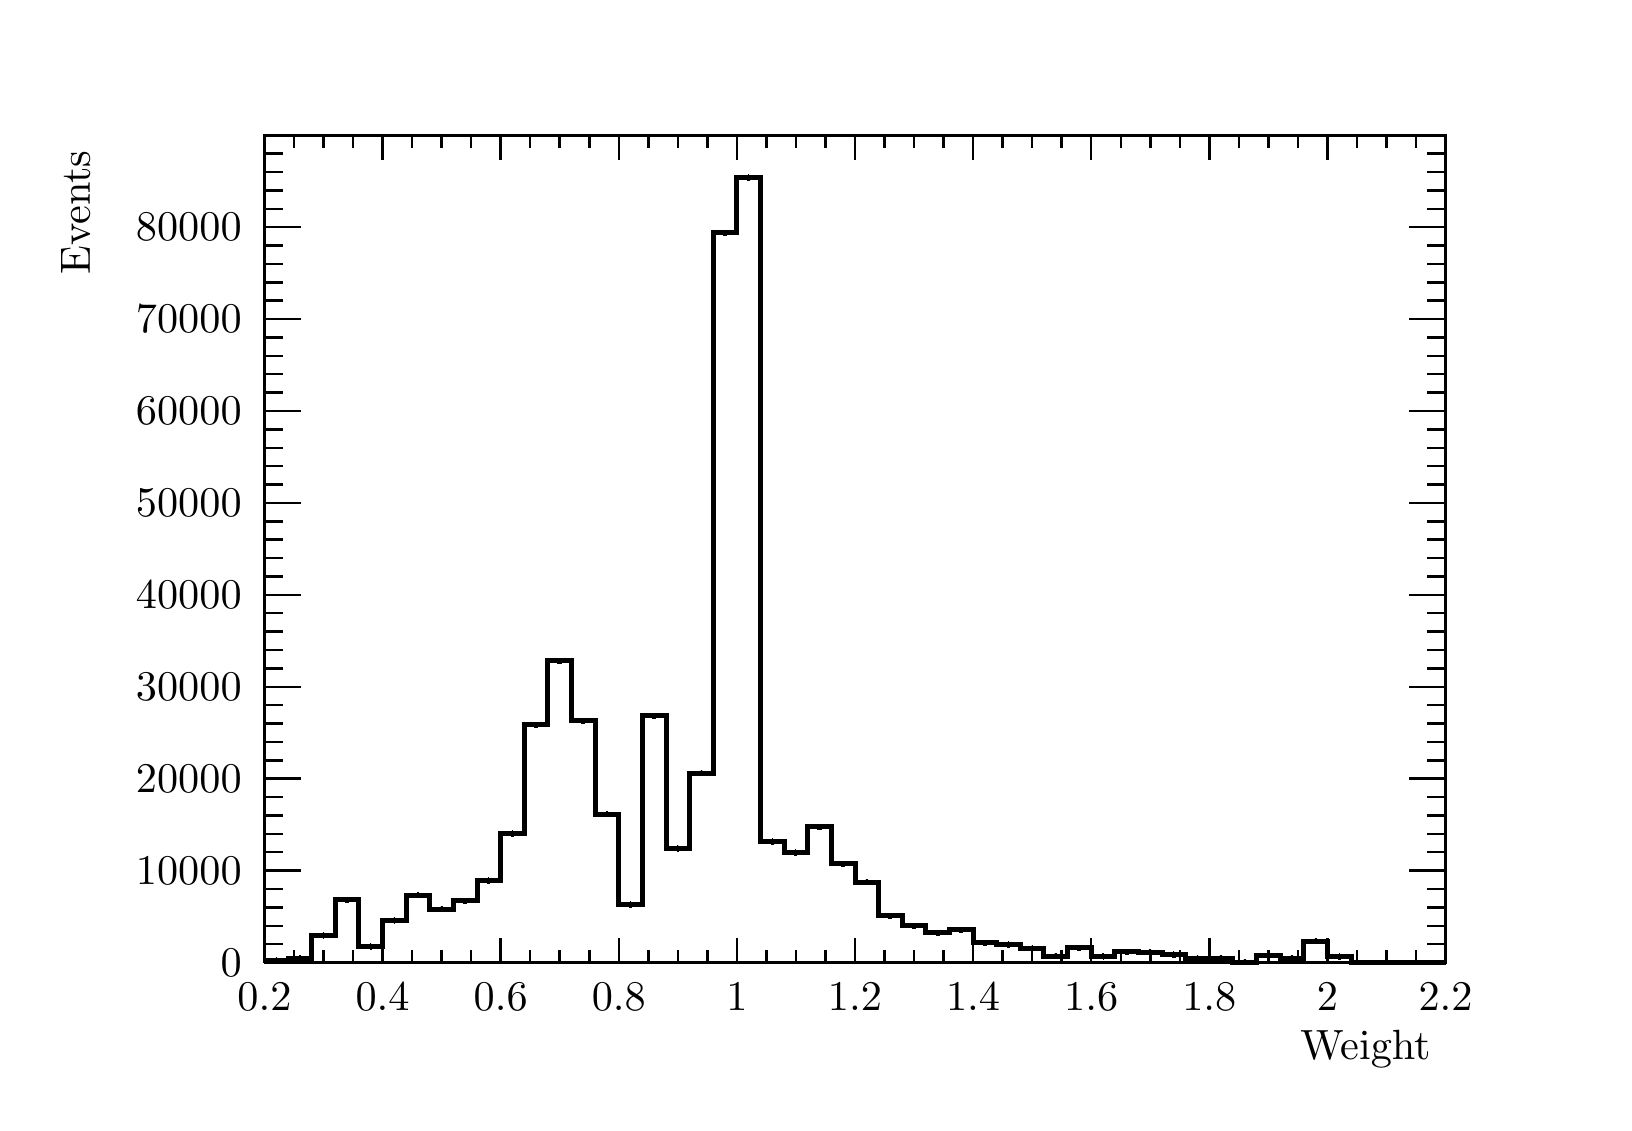
\begin{tikzpicture}
\pgfdeclareplotmark{cross} {
\pgfpathmoveto{\pgfpoint{-0.3\pgfplotmarksize}{\pgfplotmarksize}}
\pgfpathlineto{\pgfpoint{+0.3\pgfplotmarksize}{\pgfplotmarksize}}
\pgfpathlineto{\pgfpoint{+0.3\pgfplotmarksize}{0.3\pgfplotmarksize}}
\pgfpathlineto{\pgfpoint{+1\pgfplotmarksize}{0.3\pgfplotmarksize}}
\pgfpathlineto{\pgfpoint{+1\pgfplotmarksize}{-0.3\pgfplotmarksize}}
\pgfpathlineto{\pgfpoint{+0.3\pgfplotmarksize}{-0.3\pgfplotmarksize}}
\pgfpathlineto{\pgfpoint{+0.3\pgfplotmarksize}{-1.\pgfplotmarksize}}
\pgfpathlineto{\pgfpoint{-0.3\pgfplotmarksize}{-1.\pgfplotmarksize}}
\pgfpathlineto{\pgfpoint{-0.3\pgfplotmarksize}{-0.3\pgfplotmarksize}}
\pgfpathlineto{\pgfpoint{-1.\pgfplotmarksize}{-0.3\pgfplotmarksize}}
\pgfpathlineto{\pgfpoint{-1.\pgfplotmarksize}{0.3\pgfplotmarksize}}
\pgfpathlineto{\pgfpoint{-0.3\pgfplotmarksize}{0.3\pgfplotmarksize}}
\pgfpathclose
\pgfusepathqstroke
}
\pgfdeclareplotmark{cross*} {
\pgfpathmoveto{\pgfpoint{-0.3\pgfplotmarksize}{\pgfplotmarksize}}
\pgfpathlineto{\pgfpoint{+0.3\pgfplotmarksize}{\pgfplotmarksize}}
\pgfpathlineto{\pgfpoint{+0.3\pgfplotmarksize}{0.3\pgfplotmarksize}}
\pgfpathlineto{\pgfpoint{+1\pgfplotmarksize}{0.3\pgfplotmarksize}}
\pgfpathlineto{\pgfpoint{+1\pgfplotmarksize}{-0.3\pgfplotmarksize}}
\pgfpathlineto{\pgfpoint{+0.3\pgfplotmarksize}{-0.3\pgfplotmarksize}}
\pgfpathlineto{\pgfpoint{+0.3\pgfplotmarksize}{-1.\pgfplotmarksize}}
\pgfpathlineto{\pgfpoint{-0.3\pgfplotmarksize}{-1.\pgfplotmarksize}}
\pgfpathlineto{\pgfpoint{-0.3\pgfplotmarksize}{-0.3\pgfplotmarksize}}
\pgfpathlineto{\pgfpoint{-1.\pgfplotmarksize}{-0.3\pgfplotmarksize}}
\pgfpathlineto{\pgfpoint{-1.\pgfplotmarksize}{0.3\pgfplotmarksize}}
\pgfpathlineto{\pgfpoint{-0.3\pgfplotmarksize}{0.3\pgfplotmarksize}}
\pgfpathclose
\pgfusepathqfillstroke
}
\pgfdeclareplotmark{newstar} {
\pgfpathmoveto{\pgfqpoint{0pt}{\pgfplotmarksize}}
\pgfpathlineto{\pgfqpointpolar{44}{0.5\pgfplotmarksize}}
\pgfpathlineto{\pgfqpointpolar{18}{\pgfplotmarksize}}
\pgfpathlineto{\pgfqpointpolar{-20}{0.5\pgfplotmarksize}}
\pgfpathlineto{\pgfqpointpolar{-54}{\pgfplotmarksize}}
\pgfpathlineto{\pgfqpointpolar{-90}{0.5\pgfplotmarksize}}
\pgfpathlineto{\pgfqpointpolar{234}{\pgfplotmarksize}}
\pgfpathlineto{\pgfqpointpolar{198}{0.5\pgfplotmarksize}}
\pgfpathlineto{\pgfqpointpolar{162}{\pgfplotmarksize}}
\pgfpathlineto{\pgfqpointpolar{134}{0.5\pgfplotmarksize}}
\pgfpathclose
\pgfusepathqstroke
}
\pgfdeclareplotmark{newstar*} {
\pgfpathmoveto{\pgfqpoint{0pt}{\pgfplotmarksize}}
\pgfpathlineto{\pgfqpointpolar{44}{0.5\pgfplotmarksize}}
\pgfpathlineto{\pgfqpointpolar{18}{\pgfplotmarksize}}
\pgfpathlineto{\pgfqpointpolar{-20}{0.5\pgfplotmarksize}}
\pgfpathlineto{\pgfqpointpolar{-54}{\pgfplotmarksize}}
\pgfpathlineto{\pgfqpointpolar{-90}{0.5\pgfplotmarksize}}
\pgfpathlineto{\pgfqpointpolar{234}{\pgfplotmarksize}}
\pgfpathlineto{\pgfqpointpolar{198}{0.5\pgfplotmarksize}}
\pgfpathlineto{\pgfqpointpolar{162}{\pgfplotmarksize}}
\pgfpathlineto{\pgfqpointpolar{134}{0.5\pgfplotmarksize}}
\pgfpathclose
\pgfusepathqfillstroke
}
\definecolor{c}{rgb}{1,1,1};
\draw [color=c, fill=c] (0,0) rectangle (20,13.639);
\draw [color=c, fill=c] (3,1.77307) rectangle (18,12.2751);
\definecolor{c}{rgb}{0,0,0};
\draw [c,line width=0.9] (3,1.77307) -- (3,12.2751) -- (18,12.2751) -- (18,1.77307) -- (3,1.77307);
\definecolor{c}{rgb}{1,1,1};
\draw [color=c, fill=c] (3,1.77307) rectangle (18,12.2751);
\definecolor{c}{rgb}{0,0,0};
\draw [c,line width=0.9] (3,1.77307) -- (3,12.2751) -- (18,12.2751) -- (18,1.77307) -- (3,1.77307);
\draw [c,line width=1.8] (3.15,1.79578) -- (3.15,1.79746);
\draw [c,line width=1.8] (3.15,1.79746) -- (3.15,1.79915);
\foreach \P in {(3.15,1.79746)}{\draw[mark options={color=c,fill=c},mark size=2.402402pt, line width=0.000000pt, mark=*,mark size=1pt] plot coordinates {\P};}
\draw [c,line width=1.8] (3.45,1.82552) -- (3.45,1.82805);
\draw [c,line width=1.8] (3.45,1.82805) -- (3.45,1.83058);
\foreach \P in {(3.45,1.82805)}{\draw[mark options={color=c,fill=c},mark size=2.402402pt, line width=0.000000pt, mark=*,mark size=1pt] plot coordinates {\P};}
\draw [c,line width=1.8] (3.75,2.1118) -- (3.75,2.11815);
\draw [c,line width=1.8] (3.75,2.11815) -- (3.75,2.12449);
\foreach \P in {(3.75,2.11815)}{\draw[mark options={color=c,fill=c},mark size=2.402402pt, line width=0.000000pt, mark=*,mark size=1pt] plot coordinates {\P};}
\draw [c,line width=1.8] (4.05,2.55796) -- (4.05,2.56759);
\draw [c,line width=1.8] (4.05,2.56759) -- (4.05,2.57723);
\foreach \P in {(4.05,2.56759)}{\draw[mark options={color=c,fill=c},mark size=2.402402pt, line width=0.000000pt, mark=*,mark size=1pt] plot coordinates {\P};}
\draw [c,line width=1.8] (4.35,1.97294) -- (4.35,1.97783);
\draw [c,line width=1.8] (4.35,1.97783) -- (4.35,1.98272);
\foreach \P in {(4.35,1.97783)}{\draw[mark options={color=c,fill=c},mark size=2.402402pt, line width=0.000000pt, mark=*,mark size=1pt] plot coordinates {\P};}
\draw [c,line width=1.8] (4.65,2.30145) -- (4.65,2.30937);
\draw [c,line width=1.8] (4.65,2.30937) -- (4.65,2.31728);
\foreach \P in {(4.65,2.30937)}{\draw[mark options={color=c,fill=c},mark size=2.402402pt, line width=0.000000pt, mark=*,mark size=1pt] plot coordinates {\P};}
\draw [c,line width=1.8] (4.95,2.61808) -- (4.95,2.62807);
\draw [c,line width=1.8] (4.95,2.62807) -- (4.95,2.63806);
\foreach \P in {(4.95,2.62807)}{\draw[mark options={color=c,fill=c},mark size=2.402402pt, line width=0.000000pt, mark=*,mark size=1pt] plot coordinates {\P};}
\draw [c,line width=1.8] (5.25,2.44277) -- (5.25,2.45167);
\draw [c,line width=1.8] (5.25,2.45167) -- (5.25,2.46057);
\foreach \P in {(5.25,2.45167)}{\draw[mark options={color=c,fill=c},mark size=2.402402pt, line width=0.000000pt, mark=*,mark size=1pt] plot coordinates {\P};}
\draw [c,line width=1.8] (5.55,2.5459) -- (5.55,2.55545);
\draw [c,line width=1.8] (5.55,2.55545) -- (5.55,2.56501);
\foreach \P in {(5.55,2.55545)}{\draw[mark options={color=c,fill=c},mark size=2.402402pt, line width=0.000000pt, mark=*,mark size=1pt] plot coordinates {\P};}
\draw [c,line width=1.8] (5.85,2.80254) -- (5.85,2.81356);
\draw [c,line width=1.8] (5.85,2.81356) -- (5.85,2.82459);
\foreach \P in {(5.85,2.81356)}{\draw[mark options={color=c,fill=c},mark size=2.402402pt, line width=0.000000pt, mark=*,mark size=1pt] plot coordinates {\P};}
\draw [c,line width=1.8] (6.15,3.39686) -- (6.15,3.41069);
\draw [c,line width=1.8] (6.15,3.41069) -- (6.15,3.42451);
\foreach \P in {(6.15,3.41069)}{\draw[mark options={color=c,fill=c},mark size=2.402402pt, line width=0.000000pt, mark=*,mark size=1pt] plot coordinates {\P};}
\draw [c,line width=1.8] (6.45,4.77248) -- (6.45,4.79125);
\draw [c,line width=1.8] (6.45,4.79125) -- (6.45,4.81002);
\foreach \P in {(6.45,4.79125)}{\draw[mark options={color=c,fill=c},mark size=2.402402pt, line width=0.000000pt, mark=*,mark size=1pt] plot coordinates {\P};}
\draw [c,line width=1.8] (6.75,5.58203) -- (6.75,5.60317);
\draw [c,line width=1.8] (6.75,5.60317) -- (6.75,5.62432);
\foreach \P in {(6.75,5.60317)}{\draw[mark options={color=c,fill=c},mark size=2.402402pt, line width=0.000000pt, mark=*,mark size=1pt] plot coordinates {\P};}
\draw [c,line width=1.8] (7.05,4.82415) -- (7.05,4.84308);
\draw [c,line width=1.8] (7.05,4.84308) -- (7.05,4.86201);
\foreach \P in {(7.05,4.84308)}{\draw[mark options={color=c,fill=c},mark size=2.402402pt, line width=0.000000pt, mark=*,mark size=1pt] plot coordinates {\P};}
\draw [c,line width=1.8] (7.35,3.64264) -- (7.35,3.65747);
\draw [c,line width=1.8] (7.35,3.65747) -- (7.35,3.67231);
\foreach \P in {(7.35,3.65747)}{\draw[mark options={color=c,fill=c},mark size=2.402402pt, line width=0.000000pt, mark=*,mark size=1pt] plot coordinates {\P};}
\draw [c,line width=1.8] (7.65,2.49937) -- (7.65,2.50864);
\draw [c,line width=1.8] (7.65,2.50864) -- (7.65,2.51791);
\foreach \P in {(7.65,2.50864)}{\draw[mark options={color=c,fill=c},mark size=2.402402pt, line width=0.000000pt, mark=*,mark size=1pt] plot coordinates {\P};}
\draw [c,line width=1.8] (7.95,4.8863) -- (7.95,4.90542);
\draw [c,line width=1.8] (7.95,4.90542) -- (7.95,4.92454);
\foreach \P in {(7.95,4.90542)}{\draw[mark options={color=c,fill=c},mark size=2.402402pt, line width=0.000000pt, mark=*,mark size=1pt] plot coordinates {\P};}
\draw [c,line width=1.8] (8.25,3.21042) -- (8.25,3.22344);
\draw [c,line width=1.8] (8.25,3.22344) -- (8.25,3.23645);
\foreach \P in {(8.25,3.22344)}{\draw[mark options={color=c,fill=c},mark size=2.402402pt, line width=0.000000pt, mark=*,mark size=1pt] plot coordinates {\P};}
\draw [c,line width=1.8] (8.55,4.16126) -- (8.55,4.17802);
\draw [c,line width=1.8] (8.55,4.17802) -- (8.55,4.19477);
\foreach \P in {(8.55,4.17802)}{\draw[mark options={color=c,fill=c},mark size=2.402402pt, line width=0.000000pt, mark=*,mark size=1pt] plot coordinates {\P};}
\draw [c,line width=1.8] (8.85,11.0081) -- (8.85,11.041);
\draw [c,line width=1.8] (8.85,11.041) -- (8.85,11.0739);
\foreach \P in {(8.85,11.041)}{\draw[mark options={color=c,fill=c},mark size=2.402402pt, line width=0.000000pt, mark=*,mark size=1pt] plot coordinates {\P};}
\draw [c,line width=1.8] (9.15,11.7068) -- (9.15,11.7409);
\draw [c,line width=1.8] (9.15,11.7409) -- (9.15,11.775);
\foreach \P in {(9.15,11.7409)}{\draw[mark options={color=c,fill=c},mark size=2.402402pt, line width=0.000000pt, mark=*,mark size=1pt] plot coordinates {\P};}
\draw [c,line width=1.8] (9.45,3.29515) -- (9.45,3.30854);
\draw [c,line width=1.8] (9.45,3.30854) -- (9.45,3.32193);
\foreach \P in {(9.45,3.30854)}{\draw[mark options={color=c,fill=c},mark size=2.402402pt, line width=0.000000pt, mark=*,mark size=1pt] plot coordinates {\P};}
\draw [c,line width=1.8] (9.75,3.15604) -- (9.75,3.1688);
\draw [c,line width=1.8] (9.75,3.1688) -- (9.75,3.18157);
\foreach \P in {(9.75,3.1688)}{\draw[mark options={color=c,fill=c},mark size=2.402402pt, line width=0.000000pt, mark=*,mark size=1pt] plot coordinates {\P};}
\draw [c,line width=1.8] (10.05,3.48149) -- (10.05,3.49567);
\draw [c,line width=1.8] (10.05,3.49567) -- (10.05,3.50985);
\foreach \P in {(10.05,3.49567)}{\draw[mark options={color=c,fill=c},mark size=2.402402pt, line width=0.000000pt, mark=*,mark size=1pt] plot coordinates {\P};}
\draw [c,line width=1.8] (10.35,3.01347) -- (10.35,3.02556);
\draw [c,line width=1.8] (10.35,3.02556) -- (10.35,3.03766);
\foreach \P in {(10.35,3.02556)}{\draw[mark options={color=c,fill=c},mark size=2.402402pt, line width=0.000000pt, mark=*,mark size=1pt] plot coordinates {\P};}
\draw [c,line width=1.8] (10.65,2.78408) -- (10.65,2.795);
\draw [c,line width=1.8] (10.65,2.795) -- (10.65,2.80593);
\foreach \P in {(10.65,2.795)}{\draw[mark options={color=c,fill=c},mark size=2.402402pt, line width=0.000000pt, mark=*,mark size=1pt] plot coordinates {\P};}
\draw [c,line width=1.8] (10.95,2.35778) -- (10.95,2.3661);
\draw [c,line width=1.8] (10.95,2.3661) -- (10.95,2.37442);
\foreach \P in {(10.95,2.3661)}{\draw[mark options={color=c,fill=c},mark size=2.402402pt, line width=0.000000pt, mark=*,mark size=1pt] plot coordinates {\P};}
\draw [c,line width=1.8] (11.25,2.23241) -- (11.25,2.23979);
\draw [c,line width=1.8] (11.25,2.23979) -- (11.25,2.24717);
\foreach \P in {(11.25,2.23979)}{\draw[mark options={color=c,fill=c},mark size=2.402402pt, line width=0.000000pt, mark=*,mark size=1pt] plot coordinates {\P};}
\draw [c,line width=1.8] (11.55,2.14454) -- (11.55,2.15119);
\draw [c,line width=1.8] (11.55,2.15119) -- (11.55,2.15783);
\foreach \P in {(11.55,2.15119)}{\draw[mark options={color=c,fill=c},mark size=2.402402pt, line width=0.000000pt, mark=*,mark size=1pt] plot coordinates {\P};}
\draw [c,line width=1.8] (11.85,2.18042) -- (11.85,2.18737);
\draw [c,line width=1.8] (11.85,2.18737) -- (11.85,2.19433);
\foreach \P in {(11.85,2.18737)}{\draw[mark options={color=c,fill=c},mark size=2.402402pt, line width=0.000000pt, mark=*,mark size=1pt] plot coordinates {\P};}
\draw [c,line width=1.8] (12.15,2.0161) -- (12.15,2.02149);
\draw [c,line width=1.8] (12.15,2.02149) -- (12.15,2.02687);
\foreach \P in {(12.15,2.02149)}{\draw[mark options={color=c,fill=c},mark size=2.402402pt, line width=0.000000pt, mark=*,mark size=1pt] plot coordinates {\P};}
\draw [c,line width=1.8] (12.45,1.99636) -- (12.45,2.00152);
\draw [c,line width=1.8] (12.45,2.00152) -- (12.45,2.00669);
\foreach \P in {(12.45,2.00152)}{\draw[mark options={color=c,fill=c},mark size=2.402402pt, line width=0.000000pt, mark=*,mark size=1pt] plot coordinates {\P};}
\draw [c,line width=1.8] (12.75,1.94815) -- (12.75,1.95273);
\draw [c,line width=1.8] (12.75,1.95273) -- (12.75,1.95731);
\foreach \P in {(12.75,1.95273)}{\draw[mark options={color=c,fill=c},mark size=2.402402pt, line width=0.000000pt, mark=*,mark size=1pt] plot coordinates {\P};}
\draw [c,line width=1.8] (13.05,1.85238) -- (13.05,1.85548);
\draw [c,line width=1.8] (13.05,1.85548) -- (13.05,1.85859);
\foreach \P in {(13.05,1.85548)}{\draw[mark options={color=c,fill=c},mark size=2.402402pt, line width=0.000000pt, mark=*,mark size=1pt] plot coordinates {\P};}
\draw [c,line width=1.8] (13.35,1.95529) -- (13.35,1.95997);
\draw [c,line width=1.8] (13.35,1.95997) -- (13.35,1.96464);
\foreach \P in {(13.35,1.95997)}{\draw[mark options={color=c,fill=c},mark size=2.402402pt, line width=0.000000pt, mark=*,mark size=1pt] plot coordinates {\P};}
\draw [c,line width=1.8] (13.65,1.85021) -- (13.65,1.85327);
\draw [c,line width=1.8] (13.65,1.85327) -- (13.65,1.85633);
\foreach \P in {(13.65,1.85327)}{\draw[mark options={color=c,fill=c},mark size=2.402402pt, line width=0.000000pt, mark=*,mark size=1pt] plot coordinates {\P};}
\draw [c,line width=1.8] (13.95,1.90462) -- (13.95,1.9086);
\draw [c,line width=1.8] (13.95,1.9086) -- (13.95,1.91258);
\foreach \P in {(13.95,1.9086)}{\draw[mark options={color=c,fill=c},mark size=2.402402pt, line width=0.000000pt, mark=*,mark size=1pt] plot coordinates {\P};}
\draw [c,line width=1.8] (14.25,1.90048) -- (14.25,1.9044);
\draw [c,line width=1.8] (14.25,1.9044) -- (14.25,1.90831);
\foreach \P in {(14.25,1.9044)}{\draw[mark options={color=c,fill=c},mark size=2.402402pt, line width=0.000000pt, mark=*,mark size=1pt] plot coordinates {\P};}
\draw [c,line width=1.8] (14.55,1.86924) -- (14.55,1.87264);
\draw [c,line width=1.8] (14.55,1.87264) -- (14.55,1.87605);
\foreach \P in {(14.55,1.87264)}{\draw[mark options={color=c,fill=c},mark size=2.402402pt, line width=0.000000pt, mark=*,mark size=1pt] plot coordinates {\P};}
\draw [c,line width=1.8] (14.85,1.82426) -- (14.85,1.82677);
\draw [c,line width=1.8] (14.85,1.82677) -- (14.85,1.82927);
\foreach \P in {(14.85,1.82677)}{\draw[mark options={color=c,fill=c},mark size=2.402402pt, line width=0.000000pt, mark=*,mark size=1pt] plot coordinates {\P};}
\draw [c,line width=1.8] (15.15,1.82734) -- (15.15,1.82992);
\draw [c,line width=1.8] (15.15,1.82992) -- (15.15,1.83249);
\foreach \P in {(15.15,1.82992)}{\draw[mark options={color=c,fill=c},mark size=2.402402pt, line width=0.000000pt, mark=*,mark size=1pt] plot coordinates {\P};}
\draw [c,line width=1.8] (15.45,1.77786) -- (15.45,1.77867);
\draw [c,line width=1.8] (15.45,1.77867) -- (15.45,1.77948);
\foreach \P in {(15.45,1.77867)}{\draw[mark options={color=c,fill=c},mark size=2.402402pt, line width=0.000000pt, mark=*,mark size=1pt] plot coordinates {\P};}
\draw [c,line width=1.8] (15.75,1.85742) -- (15.75,1.86062);
\draw [c,line width=1.8] (15.75,1.86062) -- (15.75,1.86382);
\foreach \P in {(15.75,1.86062)}{\draw[mark options={color=c,fill=c},mark size=2.402402pt, line width=0.000000pt, mark=*,mark size=1pt] plot coordinates {\P};}
\draw [c,line width=1.8] (16.05,1.8278) -- (16.05,1.83038);
\draw [c,line width=1.8] (16.05,1.83038) -- (16.05,1.83297);
\foreach \P in {(16.05,1.83038)}{\draw[mark options={color=c,fill=c},mark size=2.402402pt, line width=0.000000pt, mark=*,mark size=1pt] plot coordinates {\P};}
\draw [c,line width=1.8] (16.35,2.03955) -- (16.35,2.04519);
\draw [c,line width=1.8] (16.35,2.04519) -- (16.35,2.05082);
\foreach \P in {(16.35,2.04519)}{\draw[mark options={color=c,fill=c},mark size=2.402402pt, line width=0.000000pt, mark=*,mark size=1pt] plot coordinates {\P};}
\draw [c,line width=1.8] (16.65,1.84437) -- (16.65,1.84731);
\draw [c,line width=1.8] (16.65,1.84731) -- (16.65,1.85026);
\foreach \P in {(16.65,1.84731)}{\draw[mark options={color=c,fill=c},mark size=2.402402pt, line width=0.000000pt, mark=*,mark size=1pt] plot coordinates {\P};}
\draw [c,line width=1.8] (3,1.79746) -- (3.3,1.79746) -- (3.3,1.82805) -- (3.6,1.82805) -- (3.6,2.11815) -- (3.9,2.11815) -- (3.9,2.56759) -- (4.2,2.56759) -- (4.2,1.97783) -- (4.5,1.97783) -- (4.5,2.30937) -- (4.8,2.30937) -- (4.8,2.62807) --
 (5.1,2.62807) -- (5.1,2.45167) -- (5.4,2.45167) -- (5.4,2.55545) -- (5.7,2.55545) -- (5.7,2.81356) -- (6,2.81356) -- (6,3.41069) -- (6.3,3.41069) -- (6.3,4.79125) -- (6.6,4.79125) -- (6.6,5.60317) -- (6.9,5.60317) -- (6.9,4.84308) -- (7.2,4.84308)
 -- (7.2,3.65747) -- (7.5,3.65747) -- (7.5,2.50864) -- (7.8,2.50864) -- (7.8,4.90542) -- (8.1,4.90542) -- (8.1,3.22344) -- (8.4,3.22344) -- (8.4,4.17802) -- (8.7,4.17802) -- (8.7,11.041) -- (9,11.041) -- (9,11.7409) -- (9.3,11.7409) -- (9.3,3.30854)
 -- (9.6,3.30854) -- (9.6,3.1688) -- (9.9,3.1688) -- (9.9,3.49567) -- (10.2,3.49567) -- (10.2,3.02556) -- (10.5,3.02556) -- (10.5,2.795) -- (10.8,2.795) -- (10.8,2.3661) -- (11.1,2.3661) -- (11.1,2.23979) -- (11.4,2.23979) -- (11.4,2.15119) --
 (11.7,2.15119) -- (11.7,2.18737) -- (12,2.18737) -- (12,2.02149) -- (12.3,2.02149) -- (12.3,2.00152) -- (12.6,2.00152) -- (12.6,1.95273) -- (12.9,1.95273) -- (12.9,1.85548) -- (13.2,1.85548) -- (13.2,1.95997) -- (13.5,1.95997) -- (13.5,1.85327) --
 (13.8,1.85327) -- (13.8,1.9086) -- (14.1,1.9086) -- (14.1,1.9044) -- (14.4,1.9044) -- (14.4,1.87264) -- (14.7,1.87264) -- (14.7,1.82677) -- (15,1.82677) -- (15,1.82992) -- (15.3,1.82992) -- (15.3,1.77867) -- (15.6,1.77867) -- (15.6,1.86062) --
 (15.9,1.86062) -- (15.9,1.83038) -- (16.2,1.83038) -- (16.2,2.04519) -- (16.5,2.04519) -- (16.5,1.84731) -- (16.8,1.84731) -- (16.8,1.77307) -- (17.1,1.77307) -- (17.1,1.77307) -- (17.4,1.77307) -- (17.4,1.77307) -- (17.7,1.77307) -- (17.7,1.77307)
 -- (18,1.77307);
\draw [c,line width=0.9] (3,1.77307) -- (18,1.77307);
\draw [c,line width=0.9] (3,2.07994) -- (3,1.77307);
\draw [c,line width=0.9] (3.375,1.9265) -- (3.375,1.77307);
\draw [c,line width=0.9] (3.75,1.9265) -- (3.75,1.77307);
\draw [c,line width=0.9] (4.125,1.9265) -- (4.125,1.77307);
\draw [c,line width=0.9] (4.5,2.07994) -- (4.5,1.77307);
\draw [c,line width=0.9] (4.875,1.9265) -- (4.875,1.77307);
\draw [c,line width=0.9] (5.25,1.9265) -- (5.25,1.77307);
\draw [c,line width=0.9] (5.625,1.9265) -- (5.625,1.77307);
\draw [c,line width=0.9] (6,2.07994) -- (6,1.77307);
\draw [c,line width=0.9] (6.375,1.9265) -- (6.375,1.77307);
\draw [c,line width=0.9] (6.75,1.9265) -- (6.75,1.77307);
\draw [c,line width=0.9] (7.125,1.9265) -- (7.125,1.77307);
\draw [c,line width=0.9] (7.5,2.07994) -- (7.5,1.77307);
\draw [c,line width=0.9] (7.875,1.9265) -- (7.875,1.77307);
\draw [c,line width=0.9] (8.25,1.9265) -- (8.25,1.77307);
\draw [c,line width=0.9] (8.625,1.9265) -- (8.625,1.77307);
\draw [c,line width=0.9] (9,2.07994) -- (9,1.77307);
\draw [c,line width=0.9] (9.375,1.9265) -- (9.375,1.77307);
\draw [c,line width=0.9] (9.75,1.9265) -- (9.75,1.77307);
\draw [c,line width=0.9] (10.125,1.9265) -- (10.125,1.77307);
\draw [c,line width=0.9] (10.5,2.07994) -- (10.5,1.77307);
\draw [c,line width=0.9] (10.875,1.9265) -- (10.875,1.77307);
\draw [c,line width=0.9] (11.25,1.9265) -- (11.25,1.77307);
\draw [c,line width=0.9] (11.625,1.9265) -- (11.625,1.77307);
\draw [c,line width=0.9] (12,2.07994) -- (12,1.77307);
\draw [c,line width=0.9] (12.375,1.9265) -- (12.375,1.77307);
\draw [c,line width=0.9] (12.75,1.9265) -- (12.75,1.77307);
\draw [c,line width=0.9] (13.125,1.9265) -- (13.125,1.77307);
\draw [c,line width=0.9] (13.5,2.07994) -- (13.5,1.77307);
\draw [c,line width=0.9] (13.875,1.9265) -- (13.875,1.77307);
\draw [c,line width=0.9] (14.25,1.9265) -- (14.25,1.77307);
\draw [c,line width=0.9] (14.625,1.9265) -- (14.625,1.77307);
\draw [c,line width=0.9] (15,2.07994) -- (15,1.77307);
\draw [c,line width=0.9] (15.375,1.9265) -- (15.375,1.77307);
\draw [c,line width=0.9] (15.75,1.9265) -- (15.75,1.77307);
\draw [c,line width=0.9] (16.125,1.9265) -- (16.125,1.77307);
\draw [c,line width=0.9] (16.5,2.07994) -- (16.5,1.77307);
\draw [c,line width=0.9] (16.875,1.9265) -- (16.875,1.77307);
\draw [c,line width=0.9] (17.25,1.9265) -- (17.25,1.77307);
\draw [c,line width=0.9] (17.625,1.9265) -- (17.625,1.77307);
\draw [c,line width=0.9] (18,2.07994) -- (18,1.77307);
\draw [anchor=base] (3,1.15931) node[scale=1.52731, color=c, rotate=0]{0.2};
\draw [anchor=base] (4.5,1.15931) node[scale=1.52731, color=c, rotate=0]{0.4};
\draw [anchor=base] (6,1.15931) node[scale=1.52731, color=c, rotate=0]{0.6};
\draw [anchor=base] (7.5,1.15931) node[scale=1.52731, color=c, rotate=0]{0.8};
\draw [anchor=base] (9,1.15931) node[scale=1.52731, color=c, rotate=0]{1};
\draw [anchor=base] (10.5,1.15931) node[scale=1.52731, color=c, rotate=0]{1.2};
\draw [anchor=base] (12,1.15931) node[scale=1.52731, color=c, rotate=0]{1.4};
\draw [anchor=base] (13.5,1.15931) node[scale=1.52731, color=c, rotate=0]{1.6};
\draw [anchor=base] (15,1.15931) node[scale=1.52731, color=c, rotate=0]{1.8};
\draw [anchor=base] (16.5,1.15931) node[scale=1.52731, color=c, rotate=0]{2};
\draw [anchor=base] (18,1.15931) node[scale=1.52731, color=c, rotate=0]{2.2};
\draw [anchor= east] (18,0.681948) node[scale=1.52731, color=c, rotate=0]{ Weight};
\draw [c,line width=0.9] (3,12.2751) -- (18,12.2751);
\draw [c,line width=0.9] (3,11.9682) -- (3,12.2751);
\draw [c,line width=0.9] (3.375,12.1216) -- (3.375,12.2751);
\draw [c,line width=0.9] (3.75,12.1216) -- (3.75,12.2751);
\draw [c,line width=0.9] (4.125,12.1216) -- (4.125,12.2751);
\draw [c,line width=0.9] (4.5,11.9682) -- (4.5,12.2751);
\draw [c,line width=0.9] (4.875,12.1216) -- (4.875,12.2751);
\draw [c,line width=0.9] (5.25,12.1216) -- (5.25,12.2751);
\draw [c,line width=0.9] (5.625,12.1216) -- (5.625,12.2751);
\draw [c,line width=0.9] (6,11.9682) -- (6,12.2751);
\draw [c,line width=0.9] (6.375,12.1216) -- (6.375,12.2751);
\draw [c,line width=0.9] (6.75,12.1216) -- (6.75,12.2751);
\draw [c,line width=0.9] (7.125,12.1216) -- (7.125,12.2751);
\draw [c,line width=0.9] (7.5,11.9682) -- (7.5,12.2751);
\draw [c,line width=0.9] (7.875,12.1216) -- (7.875,12.2751);
\draw [c,line width=0.9] (8.25,12.1216) -- (8.25,12.2751);
\draw [c,line width=0.9] (8.625,12.1216) -- (8.625,12.2751);
\draw [c,line width=0.9] (9,11.9682) -- (9,12.2751);
\draw [c,line width=0.9] (9.375,12.1216) -- (9.375,12.2751);
\draw [c,line width=0.9] (9.75,12.1216) -- (9.75,12.2751);
\draw [c,line width=0.9] (10.125,12.1216) -- (10.125,12.2751);
\draw [c,line width=0.9] (10.5,11.9682) -- (10.5,12.2751);
\draw [c,line width=0.9] (10.875,12.1216) -- (10.875,12.2751);
\draw [c,line width=0.9] (11.25,12.1216) -- (11.25,12.2751);
\draw [c,line width=0.9] (11.625,12.1216) -- (11.625,12.2751);
\draw [c,line width=0.9] (12,11.9682) -- (12,12.2751);
\draw [c,line width=0.9] (12.375,12.1216) -- (12.375,12.2751);
\draw [c,line width=0.9] (12.75,12.1216) -- (12.75,12.2751);
\draw [c,line width=0.9] (13.125,12.1216) -- (13.125,12.2751);
\draw [c,line width=0.9] (13.5,11.9682) -- (13.5,12.2751);
\draw [c,line width=0.9] (13.875,12.1216) -- (13.875,12.2751);
\draw [c,line width=0.9] (14.25,12.1216) -- (14.25,12.2751);
\draw [c,line width=0.9] (14.625,12.1216) -- (14.625,12.2751);
\draw [c,line width=0.9] (15,11.9682) -- (15,12.2751);
\draw [c,line width=0.9] (15.375,12.1216) -- (15.375,12.2751);
\draw [c,line width=0.9] (15.75,12.1216) -- (15.75,12.2751);
\draw [c,line width=0.9] (16.125,12.1216) -- (16.125,12.2751);
\draw [c,line width=0.9] (16.5,11.9682) -- (16.5,12.2751);
\draw [c,line width=0.9] (16.875,12.1216) -- (16.875,12.2751);
\draw [c,line width=0.9] (17.25,12.1216) -- (17.25,12.2751);
\draw [c,line width=0.9] (17.625,12.1216) -- (17.625,12.2751);
\draw [c,line width=0.9] (18,11.9682) -- (18,12.2751);
\draw [c,line width=0.9] (3,1.77307) -- (3,12.2751);
\draw [c,line width=0.9] (3.462,1.77307) -- (3,1.77307);
\draw [c,line width=0.9] (3.231,2.00654) -- (3,2.00654);
\draw [c,line width=0.9] (3.231,2.24002) -- (3,2.24002);
\draw [c,line width=0.9] (3.231,2.4735) -- (3,2.4735);
\draw [c,line width=0.9] (3.231,2.70698) -- (3,2.70698);
\draw [c,line width=0.9] (3.462,2.94046) -- (3,2.94046);
\draw [c,line width=0.9] (3.231,3.17394) -- (3,3.17394);
\draw [c,line width=0.9] (3.231,3.40742) -- (3,3.40742);
\draw [c,line width=0.9] (3.231,3.6409) -- (3,3.6409);
\draw [c,line width=0.9] (3.231,3.87438) -- (3,3.87438);
\draw [c,line width=0.9] (3.462,4.10785) -- (3,4.10785);
\draw [c,line width=0.9] (3.231,4.34133) -- (3,4.34133);
\draw [c,line width=0.9] (3.231,4.57481) -- (3,4.57481);
\draw [c,line width=0.9] (3.231,4.80829) -- (3,4.80829);
\draw [c,line width=0.9] (3.231,5.04177) -- (3,5.04177);
\draw [c,line width=0.9] (3.462,5.27525) -- (3,5.27525);
\draw [c,line width=0.9] (3.231,5.50873) -- (3,5.50873);
\draw [c,line width=0.9] (3.231,5.74221) -- (3,5.74221);
\draw [c,line width=0.9] (3.231,5.97569) -- (3,5.97569);
\draw [c,line width=0.9] (3.231,6.20917) -- (3,6.20917);
\draw [c,line width=0.9] (3.462,6.44264) -- (3,6.44264);
\draw [c,line width=0.9] (3.231,6.67612) -- (3,6.67612);
\draw [c,line width=0.9] (3.231,6.9096) -- (3,6.9096);
\draw [c,line width=0.9] (3.231,7.14308) -- (3,7.14308);
\draw [c,line width=0.9] (3.231,7.37656) -- (3,7.37656);
\draw [c,line width=0.9] (3.462,7.61004) -- (3,7.61004);
\draw [c,line width=0.9] (3.231,7.84352) -- (3,7.84352);
\draw [c,line width=0.9] (3.231,8.077) -- (3,8.077);
\draw [c,line width=0.9] (3.231,8.31048) -- (3,8.31048);
\draw [c,line width=0.9] (3.231,8.54395) -- (3,8.54395);
\draw [c,line width=0.9] (3.462,8.77743) -- (3,8.77743);
\draw [c,line width=0.9] (3.231,9.01091) -- (3,9.01091);
\draw [c,line width=0.9] (3.231,9.24439) -- (3,9.24439);
\draw [c,line width=0.9] (3.231,9.47787) -- (3,9.47787);
\draw [c,line width=0.9] (3.231,9.71135) -- (3,9.71135);
\draw [c,line width=0.9] (3.462,9.94483) -- (3,9.94483);
\draw [c,line width=0.9] (3.231,10.1783) -- (3,10.1783);
\draw [c,line width=0.9] (3.231,10.4118) -- (3,10.4118);
\draw [c,line width=0.9] (3.231,10.6453) -- (3,10.6453);
\draw [c,line width=0.9] (3.231,10.8787) -- (3,10.8787);
\draw [c,line width=0.9] (3.462,11.1122) -- (3,11.1122);
\draw [c,line width=0.9] (3.462,11.1122) -- (3,11.1122);
\draw [c,line width=0.9] (3.231,11.3457) -- (3,11.3457);
\draw [c,line width=0.9] (3.231,11.5792) -- (3,11.5792);
\draw [c,line width=0.9] (3.231,11.8127) -- (3,11.8127);
\draw [c,line width=0.9] (3.231,12.0461) -- (3,12.0461);
\draw [anchor= east] (2.9,1.77307) node[scale=1.52731, color=c, rotate=0]{0};
\draw [anchor= east] (2.9,2.94046) node[scale=1.52731, color=c, rotate=0]{10000};
\draw [anchor= east] (2.9,4.10785) node[scale=1.52731, color=c, rotate=0]{20000};
\draw [anchor= east] (2.9,5.27525) node[scale=1.52731, color=c, rotate=0]{30000};
\draw [anchor= east] (2.9,6.44264) node[scale=1.52731, color=c, rotate=0]{40000};
\draw [anchor= east] (2.9,7.61004) node[scale=1.52731, color=c, rotate=0]{50000};
\draw [anchor= east] (2.9,8.77743) node[scale=1.52731, color=c, rotate=0]{60000};
\draw [anchor= east] (2.9,9.94483) node[scale=1.52731, color=c, rotate=0]{70000};
\draw [anchor= east] (2.9,11.1122) node[scale=1.52731, color=c, rotate=0]{80000};
\draw [anchor= east] (0.6,12.2751) node[scale=1.52731, color=c, rotate=90]{ Events};
\draw [c,line width=0.9] (18,1.77307) -- (18,12.2751);
\draw [c,line width=0.9] (17.538,1.77307) -- (18,1.77307);
\draw [c,line width=0.9] (17.769,2.00654) -- (18,2.00654);
\draw [c,line width=0.9] (17.769,2.24002) -- (18,2.24002);
\draw [c,line width=0.9] (17.769,2.4735) -- (18,2.4735);
\draw [c,line width=0.9] (17.769,2.70698) -- (18,2.70698);
\draw [c,line width=0.9] (17.538,2.94046) -- (18,2.94046);
\draw [c,line width=0.9] (17.769,3.17394) -- (18,3.17394);
\draw [c,line width=0.9] (17.769,3.40742) -- (18,3.40742);
\draw [c,line width=0.9] (17.769,3.6409) -- (18,3.6409);
\draw [c,line width=0.9] (17.769,3.87438) -- (18,3.87438);
\draw [c,line width=0.9] (17.538,4.10785) -- (18,4.10785);
\draw [c,line width=0.9] (17.769,4.34133) -- (18,4.34133);
\draw [c,line width=0.9] (17.769,4.57481) -- (18,4.57481);
\draw [c,line width=0.9] (17.769,4.80829) -- (18,4.80829);
\draw [c,line width=0.9] (17.769,5.04177) -- (18,5.04177);
\draw [c,line width=0.9] (17.538,5.27525) -- (18,5.27525);
\draw [c,line width=0.9] (17.769,5.50873) -- (18,5.50873);
\draw [c,line width=0.9] (17.769,5.74221) -- (18,5.74221);
\draw [c,line width=0.9] (17.769,5.97569) -- (18,5.97569);
\draw [c,line width=0.9] (17.769,6.20917) -- (18,6.20917);
\draw [c,line width=0.9] (17.538,6.44264) -- (18,6.44264);
\draw [c,line width=0.9] (17.769,6.67612) -- (18,6.67612);
\draw [c,line width=0.9] (17.769,6.9096) -- (18,6.9096);
\draw [c,line width=0.9] (17.769,7.14308) -- (18,7.14308);
\draw [c,line width=0.9] (17.769,7.37656) -- (18,7.37656);
\draw [c,line width=0.9] (17.538,7.61004) -- (18,7.61004);
\draw [c,line width=0.9] (17.769,7.84352) -- (18,7.84352);
\draw [c,line width=0.9] (17.769,8.077) -- (18,8.077);
\draw [c,line width=0.9] (17.769,8.31048) -- (18,8.31048);
\draw [c,line width=0.9] (17.769,8.54395) -- (18,8.54395);
\draw [c,line width=0.9] (17.538,8.77743) -- (18,8.77743);
\draw [c,line width=0.9] (17.769,9.01091) -- (18,9.01091);
\draw [c,line width=0.9] (17.769,9.24439) -- (18,9.24439);
\draw [c,line width=0.9] (17.769,9.47787) -- (18,9.47787);
\draw [c,line width=0.9] (17.769,9.71135) -- (18,9.71135);
\draw [c,line width=0.9] (17.538,9.94483) -- (18,9.94483);
\draw [c,line width=0.9] (17.769,10.1783) -- (18,10.1783);
\draw [c,line width=0.9] (17.769,10.4118) -- (18,10.4118);
\draw [c,line width=0.9] (17.769,10.6453) -- (18,10.6453);
\draw [c,line width=0.9] (17.769,10.8787) -- (18,10.8787);
\draw [c,line width=0.9] (17.538,11.1122) -- (18,11.1122);
\draw [c,line width=0.9] (17.538,11.1122) -- (18,11.1122);
\draw [c,line width=0.9] (17.769,11.3457) -- (18,11.3457);
\draw [c,line width=0.9] (17.769,11.5792) -- (18,11.5792);
\draw [c,line width=0.9] (17.769,11.8127) -- (18,11.8127);
\draw [c,line width=0.9] (17.769,12.0461) -- (18,12.0461);
\definecolor{c}{rgb}{1,1,1};
\draw [color=c, fill=c] (2,12.8206) rectangle (18,13.5708);
\definecolor{c}{rgb}{0,0,0};
%\draw (10,13.1957) node[scale=1.40004, color=c, rotate=0]{RHC: nueswap};
\end{tikzpicture}

		\end{adjustbox}
		\caption{RHC: reco \nue}
	\end{subfigure}
	\caption[ND-GAr derived weights applied to far detector events]{ND-GAr derived weights applied to far detector events for both horn currents.}
	\label{fig:fdWeights}
\end{figure}

An example of four far detector samples with and without the reweighting, together with the mock data is shown in \citefig{fig:reweightedSamples}.
One can observe significant shifts for all the MC samples after the reweighting has been performed.

\begin{figure}[h]
	\begin{subfigure}[t]{.5\linewidth}
		\begin{adjustbox}{max totalsize=\linewidth, center}
			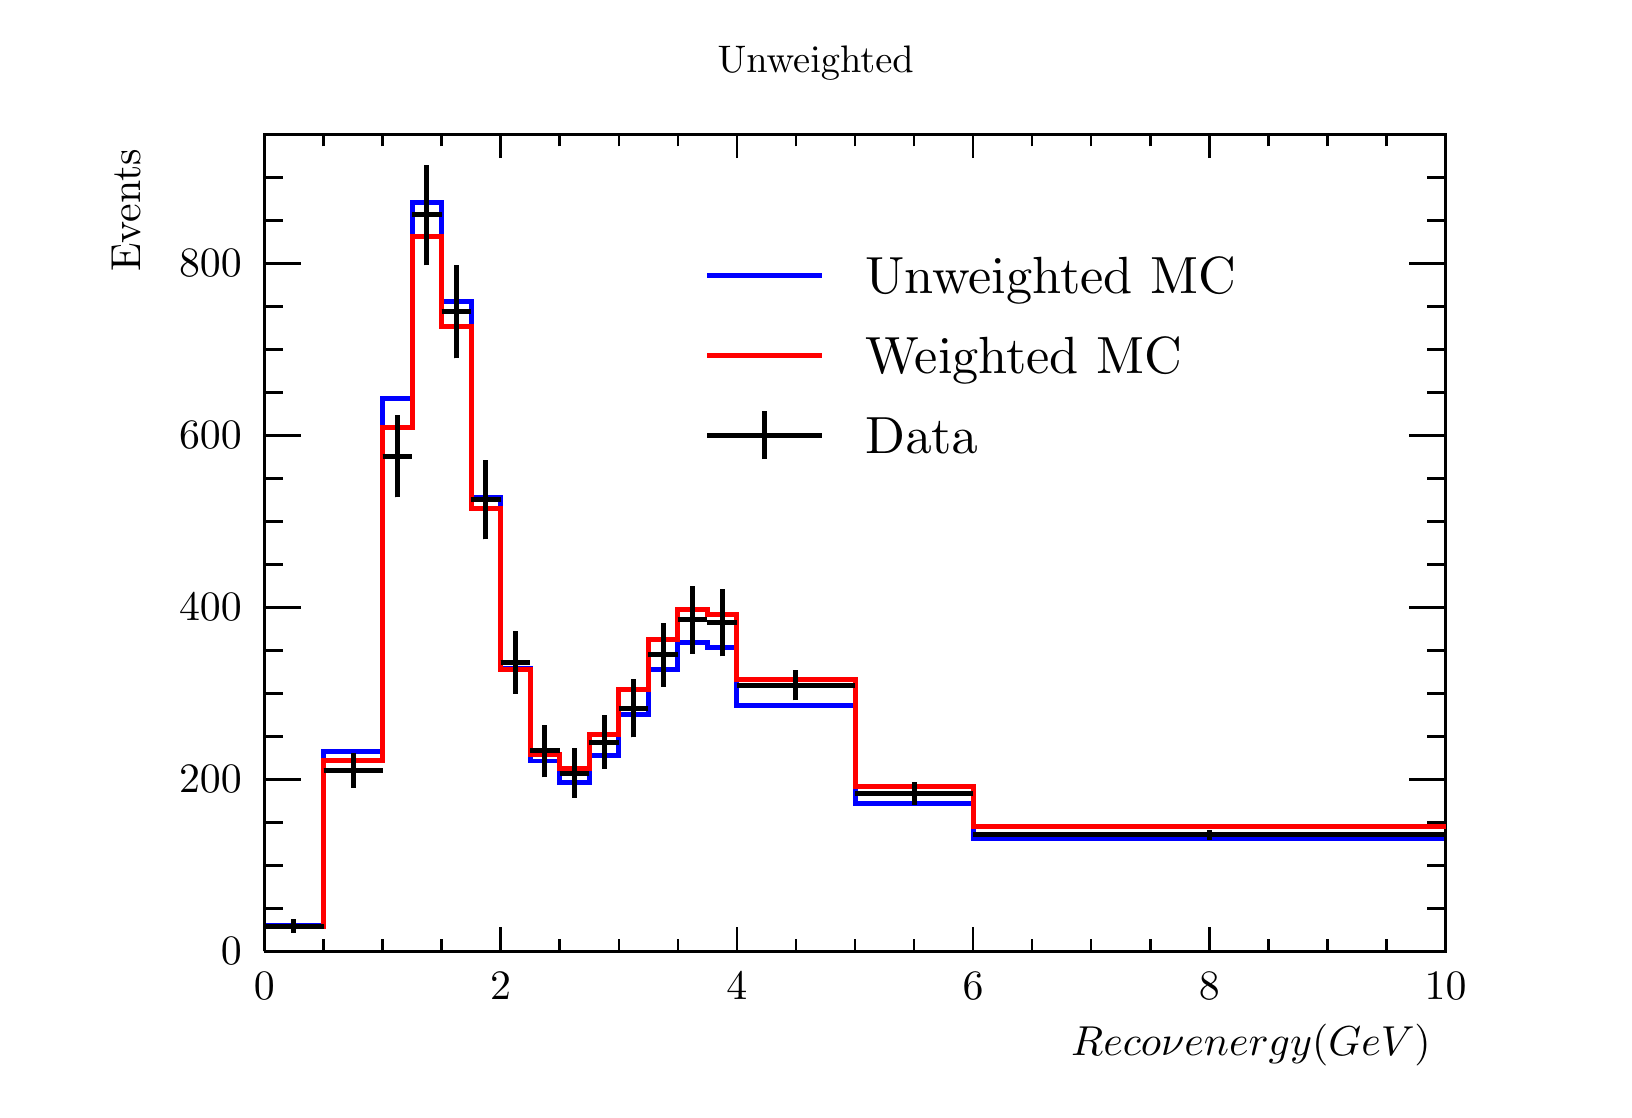
\begin{tikzpicture}
\pgfdeclareplotmark{cross} {
\pgfpathmoveto{\pgfpoint{-0.3\pgfplotmarksize}{\pgfplotmarksize}}
\pgfpathlineto{\pgfpoint{+0.3\pgfplotmarksize}{\pgfplotmarksize}}
\pgfpathlineto{\pgfpoint{+0.3\pgfplotmarksize}{0.3\pgfplotmarksize}}
\pgfpathlineto{\pgfpoint{+1\pgfplotmarksize}{0.3\pgfplotmarksize}}
\pgfpathlineto{\pgfpoint{+1\pgfplotmarksize}{-0.3\pgfplotmarksize}}
\pgfpathlineto{\pgfpoint{+0.3\pgfplotmarksize}{-0.3\pgfplotmarksize}}
\pgfpathlineto{\pgfpoint{+0.3\pgfplotmarksize}{-1.\pgfplotmarksize}}
\pgfpathlineto{\pgfpoint{-0.3\pgfplotmarksize}{-1.\pgfplotmarksize}}
\pgfpathlineto{\pgfpoint{-0.3\pgfplotmarksize}{-0.3\pgfplotmarksize}}
\pgfpathlineto{\pgfpoint{-1.\pgfplotmarksize}{-0.3\pgfplotmarksize}}
\pgfpathlineto{\pgfpoint{-1.\pgfplotmarksize}{0.3\pgfplotmarksize}}
\pgfpathlineto{\pgfpoint{-0.3\pgfplotmarksize}{0.3\pgfplotmarksize}}
\pgfpathclose
\pgfusepathqstroke
}
\pgfdeclareplotmark{cross*} {
\pgfpathmoveto{\pgfpoint{-0.3\pgfplotmarksize}{\pgfplotmarksize}}
\pgfpathlineto{\pgfpoint{+0.3\pgfplotmarksize}{\pgfplotmarksize}}
\pgfpathlineto{\pgfpoint{+0.3\pgfplotmarksize}{0.3\pgfplotmarksize}}
\pgfpathlineto{\pgfpoint{+1\pgfplotmarksize}{0.3\pgfplotmarksize}}
\pgfpathlineto{\pgfpoint{+1\pgfplotmarksize}{-0.3\pgfplotmarksize}}
\pgfpathlineto{\pgfpoint{+0.3\pgfplotmarksize}{-0.3\pgfplotmarksize}}
\pgfpathlineto{\pgfpoint{+0.3\pgfplotmarksize}{-1.\pgfplotmarksize}}
\pgfpathlineto{\pgfpoint{-0.3\pgfplotmarksize}{-1.\pgfplotmarksize}}
\pgfpathlineto{\pgfpoint{-0.3\pgfplotmarksize}{-0.3\pgfplotmarksize}}
\pgfpathlineto{\pgfpoint{-1.\pgfplotmarksize}{-0.3\pgfplotmarksize}}
\pgfpathlineto{\pgfpoint{-1.\pgfplotmarksize}{0.3\pgfplotmarksize}}
\pgfpathlineto{\pgfpoint{-0.3\pgfplotmarksize}{0.3\pgfplotmarksize}}
\pgfpathclose
\pgfusepathqfillstroke
}
\pgfdeclareplotmark{newstar} {
\pgfpathmoveto{\pgfqpoint{0pt}{\pgfplotmarksize}}
\pgfpathlineto{\pgfqpointpolar{44}{0.5\pgfplotmarksize}}
\pgfpathlineto{\pgfqpointpolar{18}{\pgfplotmarksize}}
\pgfpathlineto{\pgfqpointpolar{-20}{0.5\pgfplotmarksize}}
\pgfpathlineto{\pgfqpointpolar{-54}{\pgfplotmarksize}}
\pgfpathlineto{\pgfqpointpolar{-90}{0.5\pgfplotmarksize}}
\pgfpathlineto{\pgfqpointpolar{234}{\pgfplotmarksize}}
\pgfpathlineto{\pgfqpointpolar{198}{0.5\pgfplotmarksize}}
\pgfpathlineto{\pgfqpointpolar{162}{\pgfplotmarksize}}
\pgfpathlineto{\pgfqpointpolar{134}{0.5\pgfplotmarksize}}
\pgfpathclose
\pgfusepathqstroke
}
\pgfdeclareplotmark{newstar*} {
\pgfpathmoveto{\pgfqpoint{0pt}{\pgfplotmarksize}}
\pgfpathlineto{\pgfqpointpolar{44}{0.5\pgfplotmarksize}}
\pgfpathlineto{\pgfqpointpolar{18}{\pgfplotmarksize}}
\pgfpathlineto{\pgfqpointpolar{-20}{0.5\pgfplotmarksize}}
\pgfpathlineto{\pgfqpointpolar{-54}{\pgfplotmarksize}}
\pgfpathlineto{\pgfqpointpolar{-90}{0.5\pgfplotmarksize}}
\pgfpathlineto{\pgfqpointpolar{234}{\pgfplotmarksize}}
\pgfpathlineto{\pgfqpointpolar{198}{0.5\pgfplotmarksize}}
\pgfpathlineto{\pgfqpointpolar{162}{\pgfplotmarksize}}
\pgfpathlineto{\pgfqpointpolar{134}{0.5\pgfplotmarksize}}
\pgfpathclose
\pgfusepathqfillstroke
}
\definecolor{c}{rgb}{1,1,1};
\draw [color=c, fill=c] (0,0) rectangle (20,13.4752);
\draw [color=c, fill=c] (3,1.75177) rectangle (18,12.1277);
\definecolor{c}{rgb}{0,0,0};
\draw [c,line width=0.9] (3,1.75177) -- (3,12.1277) -- (18,12.1277) -- (18,1.75177) -- (3,1.75177);
\definecolor{c}{rgb}{1,1,1};
\draw [color=c, fill=c] (3,1.75177) rectangle (18,12.1277);
\definecolor{c}{rgb}{0,0,0};
\draw [c,line width=0.9] (3,1.75177) -- (3,12.1277) -- (18,12.1277) -- (18,1.75177) -- (3,1.75177);
\definecolor{c}{rgb}{0,0,1};
\draw [c,line width=1.8] (3,2.07958) -- (3.75,2.07958) -- (3.75,4.28523) -- (4.5,4.28523) -- (4.5,8.77265) -- (4.875,8.77265) -- (4.875,11.2649) -- (5.25,11.2649) -- (5.25,10.0098) -- (5.625,10.0098) -- (5.625,7.51667) -- (6,7.51667) -- (6,5.34596)
 -- (6.375,5.34596) -- (6.375,4.16897) -- (6.75,4.16897) -- (6.75,3.8993) -- (7.125,3.8993) -- (7.125,4.24495) -- (7.5,4.24495) -- (7.5,4.76016) -- (7.875,4.76016) -- (7.875,5.33064) -- (8.25,5.33064) -- (8.25,5.67974) -- (8.625,5.67974) --
 (8.625,5.6107) -- (9,5.6107) -- (9,4.86975) -- (10.5,4.86975) -- (10.5,3.62597) -- (12,3.62597) -- (12,3.18824) -- (18,3.18824);
\definecolor{c}{rgb}{0,0,0};
\draw [c,line width=0.9] (3,1.75177) -- (18,1.75177);
\draw [c,line width=0.9] (3,2.05496) -- (3,1.75177);
\draw [c,line width=0.9] (3.75,1.90337) -- (3.75,1.75177);
\draw [c,line width=0.9] (4.5,1.90337) -- (4.5,1.75177);
\draw [c,line width=0.9] (5.25,1.90337) -- (5.25,1.75177);
\draw [c,line width=0.9] (6,2.05496) -- (6,1.75177);
\draw [c,line width=0.9] (6.75,1.90337) -- (6.75,1.75177);
\draw [c,line width=0.9] (7.5,1.90337) -- (7.5,1.75177);
\draw [c,line width=0.9] (8.25,1.90337) -- (8.25,1.75177);
\draw [c,line width=0.9] (9,2.05496) -- (9,1.75177);
\draw [c,line width=0.9] (9.75,1.90337) -- (9.75,1.75177);
\draw [c,line width=0.9] (10.5,1.90337) -- (10.5,1.75177);
\draw [c,line width=0.9] (11.25,1.90337) -- (11.25,1.75177);
\draw [c,line width=0.9] (12,2.05496) -- (12,1.75177);
\draw [c,line width=0.9] (12.75,1.90337) -- (12.75,1.75177);
\draw [c,line width=0.9] (13.5,1.90337) -- (13.5,1.75177);
\draw [c,line width=0.9] (14.25,1.90337) -- (14.25,1.75177);
\draw [c,line width=0.9] (15,2.05496) -- (15,1.75177);
\draw [c,line width=0.9] (15.75,1.90337) -- (15.75,1.75177);
\draw [c,line width=0.9] (16.5,1.90337) -- (16.5,1.75177);
\draw [c,line width=0.9] (17.25,1.90337) -- (17.25,1.75177);
\draw [c,line width=0.9] (18,2.05496) -- (18,1.75177);
\draw [anchor=base] (3,1.14539) node[scale=1.51215, color=c, rotate=0]{0};
\draw [anchor=base] (6,1.14539) node[scale=1.51215, color=c, rotate=0]{2};
\draw [anchor=base] (9,1.14539) node[scale=1.51215, color=c, rotate=0]{4};
\draw [anchor=base] (12,1.14539) node[scale=1.51215, color=c, rotate=0]{6};
\draw [anchor=base] (15,1.14539) node[scale=1.51215, color=c, rotate=0]{8};
\draw [anchor=base] (18,1.14539) node[scale=1.51215, color=c, rotate=0]{10};
\draw [anchor= east] (18,0.565957) node[scale=1.51215, color=c, rotate=0]{$Reco \nu energy (GeV)$};
\draw [c,line width=0.9] (3,12.1277) -- (18,12.1277);
\draw [c,line width=0.9] (3,11.8245) -- (3,12.1277);
\draw [c,line width=0.9] (3.75,11.9761) -- (3.75,12.1277);
\draw [c,line width=0.9] (4.5,11.9761) -- (4.5,12.1277);
\draw [c,line width=0.9] (5.25,11.9761) -- (5.25,12.1277);
\draw [c,line width=0.9] (6,11.8245) -- (6,12.1277);
\draw [c,line width=0.9] (6.75,11.9761) -- (6.75,12.1277);
\draw [c,line width=0.9] (7.5,11.9761) -- (7.5,12.1277);
\draw [c,line width=0.9] (8.25,11.9761) -- (8.25,12.1277);
\draw [c,line width=0.9] (9,11.8245) -- (9,12.1277);
\draw [c,line width=0.9] (9.75,11.9761) -- (9.75,12.1277);
\draw [c,line width=0.9] (10.5,11.9761) -- (10.5,12.1277);
\draw [c,line width=0.9] (11.25,11.9761) -- (11.25,12.1277);
\draw [c,line width=0.9] (12,11.8245) -- (12,12.1277);
\draw [c,line width=0.9] (12.75,11.9761) -- (12.75,12.1277);
\draw [c,line width=0.9] (13.5,11.9761) -- (13.5,12.1277);
\draw [c,line width=0.9] (14.25,11.9761) -- (14.25,12.1277);
\draw [c,line width=0.9] (15,11.8245) -- (15,12.1277);
\draw [c,line width=0.9] (15.75,11.9761) -- (15.75,12.1277);
\draw [c,line width=0.9] (16.5,11.9761) -- (16.5,12.1277);
\draw [c,line width=0.9] (17.25,11.9761) -- (17.25,12.1277);
\draw [c,line width=0.9] (18,11.8245) -- (18,12.1277);
\draw [c,line width=0.9] (3,1.75177) -- (3,12.1277);
\draw [c,line width=0.9] (3.462,1.75177) -- (3,1.75177);
\draw [c,line width=0.9] (3.231,2.29787) -- (3,2.29787);
\draw [c,line width=0.9] (3.231,2.84397) -- (3,2.84397);
\draw [c,line width=0.9] (3.231,3.39007) -- (3,3.39007);
\draw [c,line width=0.9] (3.462,3.93617) -- (3,3.93617);
\draw [c,line width=0.9] (3.231,4.48227) -- (3,4.48227);
\draw [c,line width=0.9] (3.231,5.02837) -- (3,5.02837);
\draw [c,line width=0.9] (3.231,5.57447) -- (3,5.57447);
\draw [c,line width=0.9] (3.462,6.12057) -- (3,6.12057);
\draw [c,line width=0.9] (3.231,6.66667) -- (3,6.66667);
\draw [c,line width=0.9] (3.231,7.21277) -- (3,7.21277);
\draw [c,line width=0.9] (3.231,7.75887) -- (3,7.75887);
\draw [c,line width=0.9] (3.462,8.30497) -- (3,8.30497);
\draw [c,line width=0.9] (3.231,8.85106) -- (3,8.85106);
\draw [c,line width=0.9] (3.231,9.39716) -- (3,9.39716);
\draw [c,line width=0.9] (3.231,9.94326) -- (3,9.94326);
\draw [c,line width=0.9] (3.462,10.4894) -- (3,10.4894);
\draw [c,line width=0.9] (3.462,10.4894) -- (3,10.4894);
\draw [c,line width=0.9] (3.231,11.0355) -- (3,11.0355);
\draw [c,line width=0.9] (3.231,11.5816) -- (3,11.5816);
\draw [c,line width=0.9] (3.231,12.1277) -- (3,12.1277);
\draw [anchor= east] (2.9,1.75177) node[scale=1.51215, color=c, rotate=0]{0};
\draw [anchor= east] (2.9,3.93617) node[scale=1.51215, color=c, rotate=0]{200};
\draw [anchor= east] (2.9,6.12057) node[scale=1.51215, color=c, rotate=0]{400};
\draw [anchor= east] (2.9,8.30497) node[scale=1.51215, color=c, rotate=0]{600};
\draw [anchor= east] (2.9,10.4894) node[scale=1.51215, color=c, rotate=0]{800};
\draw [anchor= east] (1.24,12.1277) node[scale=1.51215, color=c, rotate=90]{Events};
\draw [c,line width=0.9] (18,1.75177) -- (18,12.1277);
\draw [c,line width=0.9] (17.538,1.75177) -- (18,1.75177);
\draw [c,line width=0.9] (17.769,2.29787) -- (18,2.29787);
\draw [c,line width=0.9] (17.769,2.84397) -- (18,2.84397);
\draw [c,line width=0.9] (17.769,3.39007) -- (18,3.39007);
\draw [c,line width=0.9] (17.538,3.93617) -- (18,3.93617);
\draw [c,line width=0.9] (17.769,4.48227) -- (18,4.48227);
\draw [c,line width=0.9] (17.769,5.02837) -- (18,5.02837);
\draw [c,line width=0.9] (17.769,5.57447) -- (18,5.57447);
\draw [c,line width=0.9] (17.538,6.12057) -- (18,6.12057);
\draw [c,line width=0.9] (17.769,6.66667) -- (18,6.66667);
\draw [c,line width=0.9] (17.769,7.21277) -- (18,7.21277);
\draw [c,line width=0.9] (17.769,7.75887) -- (18,7.75887);
\draw [c,line width=0.9] (17.538,8.30497) -- (18,8.30497);
\draw [c,line width=0.9] (17.769,8.85106) -- (18,8.85106);
\draw [c,line width=0.9] (17.769,9.39716) -- (18,9.39716);
\draw [c,line width=0.9] (17.769,9.94326) -- (18,9.94326);
\draw [c,line width=0.9] (17.538,10.4894) -- (18,10.4894);
\draw [c,line width=0.9] (17.538,10.4894) -- (18,10.4894);
\draw [c,line width=0.9] (17.769,11.0355) -- (18,11.0355);
\draw [c,line width=0.9] (17.769,11.5816) -- (18,11.5816);
\draw [c,line width=0.9] (17.769,12.1277) -- (18,12.1277);
\definecolor{c}{rgb}{1,1,1};
\draw [color=c, fill=c] (2,12.6667) rectangle (18,13.4078);
\definecolor{c}{rgb}{0,0,0};
\draw (10,13.0372) node[scale=1.38614, color=c, rotate=0]{Unweighted};
\definecolor{c}{rgb}{1,0,0};
\draw [c,line width=1.8] (3,2.06745) -- (3.75,2.06745) -- (3.75,4.16969) -- (4.5,4.16969) -- (4.5,8.40625) -- (4.875,8.40625) -- (4.875,10.8342) -- (5.25,10.8342) -- (5.25,9.68758) -- (5.625,9.68758) -- (5.625,7.37538) -- (6,7.37538) -- (6,5.33213)
 -- (6.375,5.33213) -- (6.375,4.2506) -- (6.75,4.2506) -- (6.75,4.06979) -- (7.125,4.06979) -- (7.125,4.50281) -- (7.5,4.50281) -- (7.5,5.07492) -- (7.875,5.07492) -- (7.875,5.70748) -- (8.25,5.70748) -- (8.25,6.09347) -- (8.625,6.09347) --
 (8.625,6.02772) -- (9,6.02772) -- (9,5.20555) -- (10.5,5.20555) -- (10.5,3.841) -- (12,3.841) -- (12,3.34289) -- (18,3.34289);
\definecolor{c}{rgb}{0,0,0};
\draw [c,line width=1.8] (3.375,1.98884) -- (3.375,2.07255);
\draw [c,line width=1.8] (3.375,2.07255) -- (3.375,2.15625);
\draw [c,line width=1.8] (3,2.07255) -- (3.375,2.07255);
\draw [c,line width=1.8] (3.375,2.07255) -- (3.75,2.07255);
\foreach \P in {(3.375,2.07255)}{\draw[mark options={color=c,fill=c},mark size=2.402402pt, line width=0.000000pt, mark=*,mark size=1pt] plot coordinates {\P};}
\draw [c,line width=1.8] (4.125,3.82647) -- (4.125,4.05055);
\draw [c,line width=1.8] (4.125,4.05055) -- (4.125,4.27464);
\draw [c,line width=1.8] (3.75,4.05055) -- (4.125,4.05055);
\draw [c,line width=1.8] (4.125,4.05055) -- (4.5,4.05055);
\foreach \P in {(4.125,4.05055)}{\draw[mark options={color=c,fill=c},mark size=2.402402pt, line width=0.000000pt, mark=*,mark size=1pt] plot coordinates {\P};}
\draw [c,line width=1.8] (4.6875,7.51588) -- (4.6875,8.04002);
\draw [c,line width=1.8] (4.6875,8.04002) -- (4.6875,8.56415);
\draw [c,line width=1.8] (4.5,8.04002) -- (4.6875,8.04002);
\draw [c,line width=1.8] (4.6875,8.04002) -- (4.875,8.04002);
\foreach \P in {(4.6875,8.04002)}{\draw[mark options={color=c,fill=c},mark size=2.402402pt, line width=0.000000pt, mark=*,mark size=1pt] plot coordinates {\P};}
\draw [c,line width=1.8] (5.0625,10.4658) -- (5.0625,11.1051);
\draw [c,line width=1.8] (5.0625,11.1051) -- (5.0625,11.7443);
\draw [c,line width=1.8] (4.875,11.1051) -- (5.0625,11.1051);
\draw [c,line width=1.8] (5.0625,11.1051) -- (5.25,11.1051);
\foreach \P in {(5.0625,11.1051)}{\draw[mark options={color=c,fill=c},mark size=2.402402pt, line width=0.000000pt, mark=*,mark size=1pt] plot coordinates {\P};}
\draw [c,line width=1.8] (5.4375,9.28084) -- (5.4375,9.87663);
\draw [c,line width=1.8] (5.4375,9.87663) -- (5.4375,10.4724);
\draw [c,line width=1.8] (5.25,9.87663) -- (5.4375,9.87663);
\draw [c,line width=1.8] (5.4375,9.87663) -- (5.625,9.87663);
\foreach \P in {(5.4375,9.87663)}{\draw[mark options={color=c,fill=c},mark size=2.402402pt, line width=0.000000pt, mark=*,mark size=1pt] plot coordinates {\P};}
\draw [c,line width=1.8] (5.8125,6.98507) -- (5.8125,7.48556);
\draw [c,line width=1.8] (5.8125,7.48556) -- (5.8125,7.98606);
\draw [c,line width=1.8] (5.625,7.48556) -- (5.8125,7.48556);
\draw [c,line width=1.8] (5.8125,7.48556) -- (6,7.48556);
\foreach \P in {(5.8125,7.48556)}{\draw[mark options={color=c,fill=c},mark size=2.402402pt, line width=0.000000pt, mark=*,mark size=1pt] plot coordinates {\P};}
\draw [c,line width=1.8] (6.1875,5.02255) -- (6.1875,5.42303);
\draw [c,line width=1.8] (6.1875,5.42303) -- (6.1875,5.82352);
\draw [c,line width=1.8] (6,5.42303) -- (6.1875,5.42303);
\draw [c,line width=1.8] (6.1875,5.42303) -- (6.375,5.42303);
\foreach \P in {(6.1875,5.42303)}{\draw[mark options={color=c,fill=c},mark size=2.402402pt, line width=0.000000pt, mark=*,mark size=1pt] plot coordinates {\P};}
\draw [c,line width=1.8] (6.5625,3.9634) -- (6.5625,4.29685);
\draw [c,line width=1.8] (6.5625,4.29685) -- (6.5625,4.6303);
\draw [c,line width=1.8] (6.375,4.29685) -- (6.5625,4.29685);
\draw [c,line width=1.8] (6.5625,4.29685) -- (6.75,4.29685);
\foreach \P in {(6.5625,4.29685)}{\draw[mark options={color=c,fill=c},mark size=2.402402pt, line width=0.000000pt, mark=*,mark size=1pt] plot coordinates {\P};}
\draw [c,line width=1.8] (6.9375,3.69906) -- (6.9375,4.01339);
\draw [c,line width=1.8] (6.9375,4.01339) -- (6.9375,4.32772);
\draw [c,line width=1.8] (6.75,4.01339) -- (6.9375,4.01339);
\draw [c,line width=1.8] (6.9375,4.01339) -- (7.125,4.01339);
\foreach \P in {(6.9375,4.01339)}{\draw[mark options={color=c,fill=c},mark size=2.402402pt, line width=0.000000pt, mark=*,mark size=1pt] plot coordinates {\P};}
\draw [c,line width=1.8] (7.3125,4.06819) -- (7.3125,4.4089);
\draw [c,line width=1.8] (7.3125,4.4089) -- (7.3125,4.74961);
\draw [c,line width=1.8] (7.125,4.4089) -- (7.3125,4.4089);
\draw [c,line width=1.8] (7.3125,4.4089) -- (7.5,4.4089);
\foreach \P in {(7.3125,4.4089)}{\draw[mark options={color=c,fill=c},mark size=2.402402pt, line width=0.000000pt, mark=*,mark size=1pt] plot coordinates {\P};}
\draw [c,line width=1.8] (7.6875,4.4704) -- (7.6875,4.83757);
\draw [c,line width=1.8] (7.6875,4.83757) -- (7.6875,5.20474);
\draw [c,line width=1.8] (7.5,4.83757) -- (7.6875,4.83757);
\draw [c,line width=1.8] (7.6875,4.83757) -- (7.875,4.83757);
\foreach \P in {(7.6875,4.83757)}{\draw[mark options={color=c,fill=c},mark size=2.402402pt, line width=0.000000pt, mark=*,mark size=1pt] plot coordinates {\P};}
\draw [c,line width=1.8] (8.0625,5.11203) -- (8.0625,5.51765);
\draw [c,line width=1.8] (8.0625,5.51765) -- (8.0625,5.92326);
\draw [c,line width=1.8] (7.875,5.51765) -- (8.0625,5.51765);
\draw [c,line width=1.8] (8.0625,5.51765) -- (8.25,5.51765);
\foreach \P in {(8.0625,5.51765)}{\draw[mark options={color=c,fill=c},mark size=2.402402pt, line width=0.000000pt, mark=*,mark size=1pt] plot coordinates {\P};}
\draw [c,line width=1.8] (8.4375,5.53322) -- (8.4375,5.96211);
\draw [c,line width=1.8] (8.4375,5.96211) -- (8.4375,6.39099);
\draw [c,line width=1.8] (8.25,5.96211) -- (8.4375,5.96211);
\draw [c,line width=1.8] (8.4375,5.96211) -- (8.625,5.96211);
\foreach \P in {(8.4375,5.96211)}{\draw[mark options={color=c,fill=c},mark size=2.402402pt, line width=0.000000pt, mark=*,mark size=1pt] plot coordinates {\P};}
\draw [c,line width=1.8] (8.8125,5.50016) -- (8.8125,5.92726);
\draw [c,line width=1.8] (8.8125,5.92726) -- (8.8125,6.35437);
\draw [c,line width=1.8] (8.625,5.92726) -- (8.8125,5.92726);
\draw [c,line width=1.8] (8.8125,5.92726) -- (9,5.92726);
\foreach \P in {(8.8125,5.92726)}{\draw[mark options={color=c,fill=c},mark size=2.402402pt, line width=0.000000pt, mark=*,mark size=1pt] plot coordinates {\P};}
\draw [c,line width=1.8] (9.75,4.94051) -- (9.75,5.13268);
\draw [c,line width=1.8] (9.75,5.13268) -- (9.75,5.32484);
\draw [c,line width=1.8] (9,5.13268) -- (9.75,5.13268);
\draw [c,line width=1.8] (9.75,5.13268) -- (10.5,5.13268);
\foreach \P in {(9.75,5.13268)}{\draw[mark options={color=c,fill=c},mark size=2.402402pt, line width=0.000000pt, mark=*,mark size=1pt] plot coordinates {\P};}
\draw [c,line width=1.8] (11.25,3.61156) -- (11.25,3.75965);
\draw [c,line width=1.8] (11.25,3.75965) -- (11.25,3.90773);
\draw [c,line width=1.8] (10.5,3.75965) -- (11.25,3.75965);
\draw [c,line width=1.8] (11.25,3.75965) -- (12,3.75965);
\foreach \P in {(11.25,3.75965)}{\draw[mark options={color=c,fill=c},mark size=2.402402pt, line width=0.000000pt, mark=*,mark size=1pt] plot coordinates {\P};}
\draw [c,line width=1.8] (15,3.16712) -- (15,3.23066);
\draw [c,line width=1.8] (15,3.23066) -- (15,3.29421);
\draw [c,line width=1.8] (12,3.23066) -- (15,3.23066);
\draw [c,line width=1.8] (15,3.23066) -- (18,3.23066);
\foreach \P in {(15,3.23066)}{\draw[mark options={color=c,fill=c},mark size=2.402402pt, line width=0.000000pt, mark=*,mark size=1pt] plot coordinates {\P};}
\draw [c,line width=1.8] (3.375,1.98884) -- (3.375,2.07255);
\draw [c,line width=1.8] (3.375,2.07255) -- (3.375,2.15625);
\draw [c,line width=1.8] (3,2.07255) -- (3.375,2.07255);
\draw [c,line width=1.8] (3.375,2.07255) -- (3.75,2.07255);
\foreach \P in {(3.375,2.07255)}{\draw[mark options={color=c,fill=c},mark size=2.402402pt, line width=0.000000pt, mark=*,mark size=1pt] plot coordinates {\P};}
\draw [c,line width=1.8] (4.125,3.82647) -- (4.125,4.05055);
\draw [c,line width=1.8] (4.125,4.05055) -- (4.125,4.27464);
\draw [c,line width=1.8] (3.75,4.05055) -- (4.125,4.05055);
\draw [c,line width=1.8] (4.125,4.05055) -- (4.5,4.05055);
\foreach \P in {(4.125,4.05055)}{\draw[mark options={color=c,fill=c},mark size=2.402402pt, line width=0.000000pt, mark=*,mark size=1pt] plot coordinates {\P};}
\draw [c,line width=1.8] (4.6875,7.51588) -- (4.6875,8.04002);
\draw [c,line width=1.8] (4.6875,8.04002) -- (4.6875,8.56415);
\draw [c,line width=1.8] (4.5,8.04002) -- (4.6875,8.04002);
\draw [c,line width=1.8] (4.6875,8.04002) -- (4.875,8.04002);
\foreach \P in {(4.6875,8.04002)}{\draw[mark options={color=c,fill=c},mark size=2.402402pt, line width=0.000000pt, mark=*,mark size=1pt] plot coordinates {\P};}
\draw [c,line width=1.8] (5.0625,10.4658) -- (5.0625,11.1051);
\draw [c,line width=1.8] (5.0625,11.1051) -- (5.0625,11.7443);
\draw [c,line width=1.8] (4.875,11.1051) -- (5.0625,11.1051);
\draw [c,line width=1.8] (5.0625,11.1051) -- (5.25,11.1051);
\foreach \P in {(5.0625,11.1051)}{\draw[mark options={color=c,fill=c},mark size=2.402402pt, line width=0.000000pt, mark=*,mark size=1pt] plot coordinates {\P};}
\draw [c,line width=1.8] (5.4375,9.28084) -- (5.4375,9.87663);
\draw [c,line width=1.8] (5.4375,9.87663) -- (5.4375,10.4724);
\draw [c,line width=1.8] (5.25,9.87663) -- (5.4375,9.87663);
\draw [c,line width=1.8] (5.4375,9.87663) -- (5.625,9.87663);
\foreach \P in {(5.4375,9.87663)}{\draw[mark options={color=c,fill=c},mark size=2.402402pt, line width=0.000000pt, mark=*,mark size=1pt] plot coordinates {\P};}
\draw [c,line width=1.8] (5.8125,6.98507) -- (5.8125,7.48556);
\draw [c,line width=1.8] (5.8125,7.48556) -- (5.8125,7.98606);
\draw [c,line width=1.8] (5.625,7.48556) -- (5.8125,7.48556);
\draw [c,line width=1.8] (5.8125,7.48556) -- (6,7.48556);
\foreach \P in {(5.8125,7.48556)}{\draw[mark options={color=c,fill=c},mark size=2.402402pt, line width=0.000000pt, mark=*,mark size=1pt] plot coordinates {\P};}
\draw [c,line width=1.8] (6.1875,5.02255) -- (6.1875,5.42303);
\draw [c,line width=1.8] (6.1875,5.42303) -- (6.1875,5.82352);
\draw [c,line width=1.8] (6,5.42303) -- (6.1875,5.42303);
\draw [c,line width=1.8] (6.1875,5.42303) -- (6.375,5.42303);
\foreach \P in {(6.1875,5.42303)}{\draw[mark options={color=c,fill=c},mark size=2.402402pt, line width=0.000000pt, mark=*,mark size=1pt] plot coordinates {\P};}
\draw [c,line width=1.8] (6.5625,3.9634) -- (6.5625,4.29685);
\draw [c,line width=1.8] (6.5625,4.29685) -- (6.5625,4.6303);
\draw [c,line width=1.8] (6.375,4.29685) -- (6.5625,4.29685);
\draw [c,line width=1.8] (6.5625,4.29685) -- (6.75,4.29685);
\foreach \P in {(6.5625,4.29685)}{\draw[mark options={color=c,fill=c},mark size=2.402402pt, line width=0.000000pt, mark=*,mark size=1pt] plot coordinates {\P};}
\draw [c,line width=1.8] (6.9375,3.69906) -- (6.9375,4.01339);
\draw [c,line width=1.8] (6.9375,4.01339) -- (6.9375,4.32772);
\draw [c,line width=1.8] (6.75,4.01339) -- (6.9375,4.01339);
\draw [c,line width=1.8] (6.9375,4.01339) -- (7.125,4.01339);
\foreach \P in {(6.9375,4.01339)}{\draw[mark options={color=c,fill=c},mark size=2.402402pt, line width=0.000000pt, mark=*,mark size=1pt] plot coordinates {\P};}
\draw [c,line width=1.8] (7.3125,4.06819) -- (7.3125,4.4089);
\draw [c,line width=1.8] (7.3125,4.4089) -- (7.3125,4.74961);
\draw [c,line width=1.8] (7.125,4.4089) -- (7.3125,4.4089);
\draw [c,line width=1.8] (7.3125,4.4089) -- (7.5,4.4089);
\foreach \P in {(7.3125,4.4089)}{\draw[mark options={color=c,fill=c},mark size=2.402402pt, line width=0.000000pt, mark=*,mark size=1pt] plot coordinates {\P};}
\draw [c,line width=1.8] (7.6875,4.4704) -- (7.6875,4.83757);
\draw [c,line width=1.8] (7.6875,4.83757) -- (7.6875,5.20474);
\draw [c,line width=1.8] (7.5,4.83757) -- (7.6875,4.83757);
\draw [c,line width=1.8] (7.6875,4.83757) -- (7.875,4.83757);
\foreach \P in {(7.6875,4.83757)}{\draw[mark options={color=c,fill=c},mark size=2.402402pt, line width=0.000000pt, mark=*,mark size=1pt] plot coordinates {\P};}
\draw [c,line width=1.8] (8.0625,5.11203) -- (8.0625,5.51765);
\draw [c,line width=1.8] (8.0625,5.51765) -- (8.0625,5.92326);
\draw [c,line width=1.8] (7.875,5.51765) -- (8.0625,5.51765);
\draw [c,line width=1.8] (8.0625,5.51765) -- (8.25,5.51765);
\foreach \P in {(8.0625,5.51765)}{\draw[mark options={color=c,fill=c},mark size=2.402402pt, line width=0.000000pt, mark=*,mark size=1pt] plot coordinates {\P};}
\draw [c,line width=1.8] (8.4375,5.53322) -- (8.4375,5.96211);
\draw [c,line width=1.8] (8.4375,5.96211) -- (8.4375,6.39099);
\draw [c,line width=1.8] (8.25,5.96211) -- (8.4375,5.96211);
\draw [c,line width=1.8] (8.4375,5.96211) -- (8.625,5.96211);
\foreach \P in {(8.4375,5.96211)}{\draw[mark options={color=c,fill=c},mark size=2.402402pt, line width=0.000000pt, mark=*,mark size=1pt] plot coordinates {\P};}
\draw [c,line width=1.8] (8.8125,5.50016) -- (8.8125,5.92726);
\draw [c,line width=1.8] (8.8125,5.92726) -- (8.8125,6.35437);
\draw [c,line width=1.8] (8.625,5.92726) -- (8.8125,5.92726);
\draw [c,line width=1.8] (8.8125,5.92726) -- (9,5.92726);
\foreach \P in {(8.8125,5.92726)}{\draw[mark options={color=c,fill=c},mark size=2.402402pt, line width=0.000000pt, mark=*,mark size=1pt] plot coordinates {\P};}
\draw [c,line width=1.8] (9.75,4.94051) -- (9.75,5.13268);
\draw [c,line width=1.8] (9.75,5.13268) -- (9.75,5.32484);
\draw [c,line width=1.8] (9,5.13268) -- (9.75,5.13268);
\draw [c,line width=1.8] (9.75,5.13268) -- (10.5,5.13268);
\foreach \P in {(9.75,5.13268)}{\draw[mark options={color=c,fill=c},mark size=2.402402pt, line width=0.000000pt, mark=*,mark size=1pt] plot coordinates {\P};}
\draw [c,line width=1.8] (11.25,3.61156) -- (11.25,3.75965);
\draw [c,line width=1.8] (11.25,3.75965) -- (11.25,3.90773);
\draw [c,line width=1.8] (10.5,3.75965) -- (11.25,3.75965);
\draw [c,line width=1.8] (11.25,3.75965) -- (12,3.75965);
\foreach \P in {(11.25,3.75965)}{\draw[mark options={color=c,fill=c},mark size=2.402402pt, line width=0.000000pt, mark=*,mark size=1pt] plot coordinates {\P};}
\draw [c,line width=1.8] (15,3.16712) -- (15,3.23066);
\draw [c,line width=1.8] (15,3.23066) -- (15,3.29421);
\draw [c,line width=1.8] (12,3.23066) -- (15,3.23066);
\draw [c,line width=1.8] (15,3.23066) -- (18,3.23066);
\foreach \P in {(15,3.23066)}{\draw[mark options={color=c,fill=c},mark size=2.402402pt, line width=0.000000pt, mark=*,mark size=1pt] plot coordinates {\P};}
\draw [c,line width=1.8] (3.375,1.98884) -- (3.375,2.07255);
\draw [c,line width=1.8] (3.375,2.07255) -- (3.375,2.15625);
\draw [c,line width=1.8] (3,2.07255) -- (3.375,2.07255);
\draw [c,line width=1.8] (3.375,2.07255) -- (3.75,2.07255);
\foreach \P in {(3.375,2.07255)}{\draw[mark options={color=c,fill=c},mark size=2.402402pt, line width=0.000000pt, mark=*,mark size=1pt] plot coordinates {\P};}
\draw [c,line width=1.8] (4.125,3.82647) -- (4.125,4.05055);
\draw [c,line width=1.8] (4.125,4.05055) -- (4.125,4.27464);
\draw [c,line width=1.8] (3.75,4.05055) -- (4.125,4.05055);
\draw [c,line width=1.8] (4.125,4.05055) -- (4.5,4.05055);
\foreach \P in {(4.125,4.05055)}{\draw[mark options={color=c,fill=c},mark size=2.402402pt, line width=0.000000pt, mark=*,mark size=1pt] plot coordinates {\P};}
\draw [c,line width=1.8] (4.6875,7.51588) -- (4.6875,8.04002);
\draw [c,line width=1.8] (4.6875,8.04002) -- (4.6875,8.56415);
\draw [c,line width=1.8] (4.5,8.04002) -- (4.6875,8.04002);
\draw [c,line width=1.8] (4.6875,8.04002) -- (4.875,8.04002);
\foreach \P in {(4.6875,8.04002)}{\draw[mark options={color=c,fill=c},mark size=2.402402pt, line width=0.000000pt, mark=*,mark size=1pt] plot coordinates {\P};}
\draw [c,line width=1.8] (5.0625,10.4658) -- (5.0625,11.1051);
\draw [c,line width=1.8] (5.0625,11.1051) -- (5.0625,11.7443);
\draw [c,line width=1.8] (4.875,11.1051) -- (5.0625,11.1051);
\draw [c,line width=1.8] (5.0625,11.1051) -- (5.25,11.1051);
\foreach \P in {(5.0625,11.1051)}{\draw[mark options={color=c,fill=c},mark size=2.402402pt, line width=0.000000pt, mark=*,mark size=1pt] plot coordinates {\P};}
\draw [c,line width=1.8] (5.4375,9.28084) -- (5.4375,9.87663);
\draw [c,line width=1.8] (5.4375,9.87663) -- (5.4375,10.4724);
\draw [c,line width=1.8] (5.25,9.87663) -- (5.4375,9.87663);
\draw [c,line width=1.8] (5.4375,9.87663) -- (5.625,9.87663);
\foreach \P in {(5.4375,9.87663)}{\draw[mark options={color=c,fill=c},mark size=2.402402pt, line width=0.000000pt, mark=*,mark size=1pt] plot coordinates {\P};}
\draw [c,line width=1.8] (5.8125,6.98507) -- (5.8125,7.48556);
\draw [c,line width=1.8] (5.8125,7.48556) -- (5.8125,7.98606);
\draw [c,line width=1.8] (5.625,7.48556) -- (5.8125,7.48556);
\draw [c,line width=1.8] (5.8125,7.48556) -- (6,7.48556);
\foreach \P in {(5.8125,7.48556)}{\draw[mark options={color=c,fill=c},mark size=2.402402pt, line width=0.000000pt, mark=*,mark size=1pt] plot coordinates {\P};}
\draw [c,line width=1.8] (6.1875,5.02255) -- (6.1875,5.42303);
\draw [c,line width=1.8] (6.1875,5.42303) -- (6.1875,5.82352);
\draw [c,line width=1.8] (6,5.42303) -- (6.1875,5.42303);
\draw [c,line width=1.8] (6.1875,5.42303) -- (6.375,5.42303);
\foreach \P in {(6.1875,5.42303)}{\draw[mark options={color=c,fill=c},mark size=2.402402pt, line width=0.000000pt, mark=*,mark size=1pt] plot coordinates {\P};}
\draw [c,line width=1.8] (6.5625,3.9634) -- (6.5625,4.29685);
\draw [c,line width=1.8] (6.5625,4.29685) -- (6.5625,4.6303);
\draw [c,line width=1.8] (6.375,4.29685) -- (6.5625,4.29685);
\draw [c,line width=1.8] (6.5625,4.29685) -- (6.75,4.29685);
\foreach \P in {(6.5625,4.29685)}{\draw[mark options={color=c,fill=c},mark size=2.402402pt, line width=0.000000pt, mark=*,mark size=1pt] plot coordinates {\P};}
\draw [c,line width=1.8] (6.9375,3.69906) -- (6.9375,4.01339);
\draw [c,line width=1.8] (6.9375,4.01339) -- (6.9375,4.32772);
\draw [c,line width=1.8] (6.75,4.01339) -- (6.9375,4.01339);
\draw [c,line width=1.8] (6.9375,4.01339) -- (7.125,4.01339);
\foreach \P in {(6.9375,4.01339)}{\draw[mark options={color=c,fill=c},mark size=2.402402pt, line width=0.000000pt, mark=*,mark size=1pt] plot coordinates {\P};}
\draw [c,line width=1.8] (7.3125,4.06819) -- (7.3125,4.4089);
\draw [c,line width=1.8] (7.3125,4.4089) -- (7.3125,4.74961);
\draw [c,line width=1.8] (7.125,4.4089) -- (7.3125,4.4089);
\draw [c,line width=1.8] (7.3125,4.4089) -- (7.5,4.4089);
\foreach \P in {(7.3125,4.4089)}{\draw[mark options={color=c,fill=c},mark size=2.402402pt, line width=0.000000pt, mark=*,mark size=1pt] plot coordinates {\P};}
\draw [c,line width=1.8] (7.6875,4.4704) -- (7.6875,4.83757);
\draw [c,line width=1.8] (7.6875,4.83757) -- (7.6875,5.20474);
\draw [c,line width=1.8] (7.5,4.83757) -- (7.6875,4.83757);
\draw [c,line width=1.8] (7.6875,4.83757) -- (7.875,4.83757);
\foreach \P in {(7.6875,4.83757)}{\draw[mark options={color=c,fill=c},mark size=2.402402pt, line width=0.000000pt, mark=*,mark size=1pt] plot coordinates {\P};}
\draw [c,line width=1.8] (8.0625,5.11203) -- (8.0625,5.51765);
\draw [c,line width=1.8] (8.0625,5.51765) -- (8.0625,5.92326);
\draw [c,line width=1.8] (7.875,5.51765) -- (8.0625,5.51765);
\draw [c,line width=1.8] (8.0625,5.51765) -- (8.25,5.51765);
\foreach \P in {(8.0625,5.51765)}{\draw[mark options={color=c,fill=c},mark size=2.402402pt, line width=0.000000pt, mark=*,mark size=1pt] plot coordinates {\P};}
\draw [c,line width=1.8] (8.4375,5.53322) -- (8.4375,5.96211);
\draw [c,line width=1.8] (8.4375,5.96211) -- (8.4375,6.39099);
\draw [c,line width=1.8] (8.25,5.96211) -- (8.4375,5.96211);
\draw [c,line width=1.8] (8.4375,5.96211) -- (8.625,5.96211);
\foreach \P in {(8.4375,5.96211)}{\draw[mark options={color=c,fill=c},mark size=2.402402pt, line width=0.000000pt, mark=*,mark size=1pt] plot coordinates {\P};}
\draw [c,line width=1.8] (8.8125,5.50016) -- (8.8125,5.92726);
\draw [c,line width=1.8] (8.8125,5.92726) -- (8.8125,6.35437);
\draw [c,line width=1.8] (8.625,5.92726) -- (8.8125,5.92726);
\draw [c,line width=1.8] (8.8125,5.92726) -- (9,5.92726);
\foreach \P in {(8.8125,5.92726)}{\draw[mark options={color=c,fill=c},mark size=2.402402pt, line width=0.000000pt, mark=*,mark size=1pt] plot coordinates {\P};}
\draw [c,line width=1.8] (9.75,4.94051) -- (9.75,5.13268);
\draw [c,line width=1.8] (9.75,5.13268) -- (9.75,5.32484);
\draw [c,line width=1.8] (9,5.13268) -- (9.75,5.13268);
\draw [c,line width=1.8] (9.75,5.13268) -- (10.5,5.13268);
\foreach \P in {(9.75,5.13268)}{\draw[mark options={color=c,fill=c},mark size=2.402402pt, line width=0.000000pt, mark=*,mark size=1pt] plot coordinates {\P};}
\draw [c,line width=1.8] (11.25,3.61156) -- (11.25,3.75965);
\draw [c,line width=1.8] (11.25,3.75965) -- (11.25,3.90773);
\draw [c,line width=1.8] (10.5,3.75965) -- (11.25,3.75965);
\draw [c,line width=1.8] (11.25,3.75965) -- (12,3.75965);
\foreach \P in {(11.25,3.75965)}{\draw[mark options={color=c,fill=c},mark size=2.402402pt, line width=0.000000pt, mark=*,mark size=1pt] plot coordinates {\P};}
\draw [c,line width=1.8] (15,3.16712) -- (15,3.23066);
\draw [c,line width=1.8] (15,3.23066) -- (15,3.29421);
\draw [c,line width=1.8] (12,3.23066) -- (15,3.23066);
\draw [c,line width=1.8] (15,3.23066) -- (18,3.23066);
\foreach \P in {(15,3.23066)}{\draw[mark options={color=c,fill=c},mark size=2.402402pt, line width=0.000000pt, mark=*,mark size=1pt] plot coordinates {\P};}
\definecolor{c}{rgb}{1,1,1};
\draw [color=c, fill=c] (8.31206,7.80142) rectangle (16.6525,10.8369);
\definecolor{c}{rgb}{0,0,0};
\draw [anchor=base west] (10.3972,10.1033) node[scale=1.89019, color=c, rotate=0]{Unweighted MC};
\definecolor{c}{rgb}{0,0,1};
\draw [c,line width=1.8] (8.62482,10.331) -- (10.0844,10.331);
\definecolor{c}{rgb}{0,0,0};
\draw [anchor=base west] (10.3972,9.09149) node[scale=1.89019, color=c, rotate=0]{Weighted MC};
\definecolor{c}{rgb}{1,0,0};
\draw [c,line width=1.8] (8.62482,9.31915) -- (10.0844,9.31915);
\definecolor{c}{rgb}{0,0,0};
\draw [anchor=base west] (10.3972,8.07967) node[scale=1.89019, color=c, rotate=0]{Data};
\draw [c,line width=1.8] (8.62482,8.30733) -- (10.0844,8.30733);
\draw [c,line width=1.8] (9.35461,8.00378) -- (9.35461,8.61088);
\end{tikzpicture}

		\end{adjustbox}
		\caption{FHC \numu}
	\end{subfigure}
	\hfill
	\begin{subfigure}[t]{.5\linewidth}
		\begin{adjustbox}{max totalsize=\linewidth, center}
			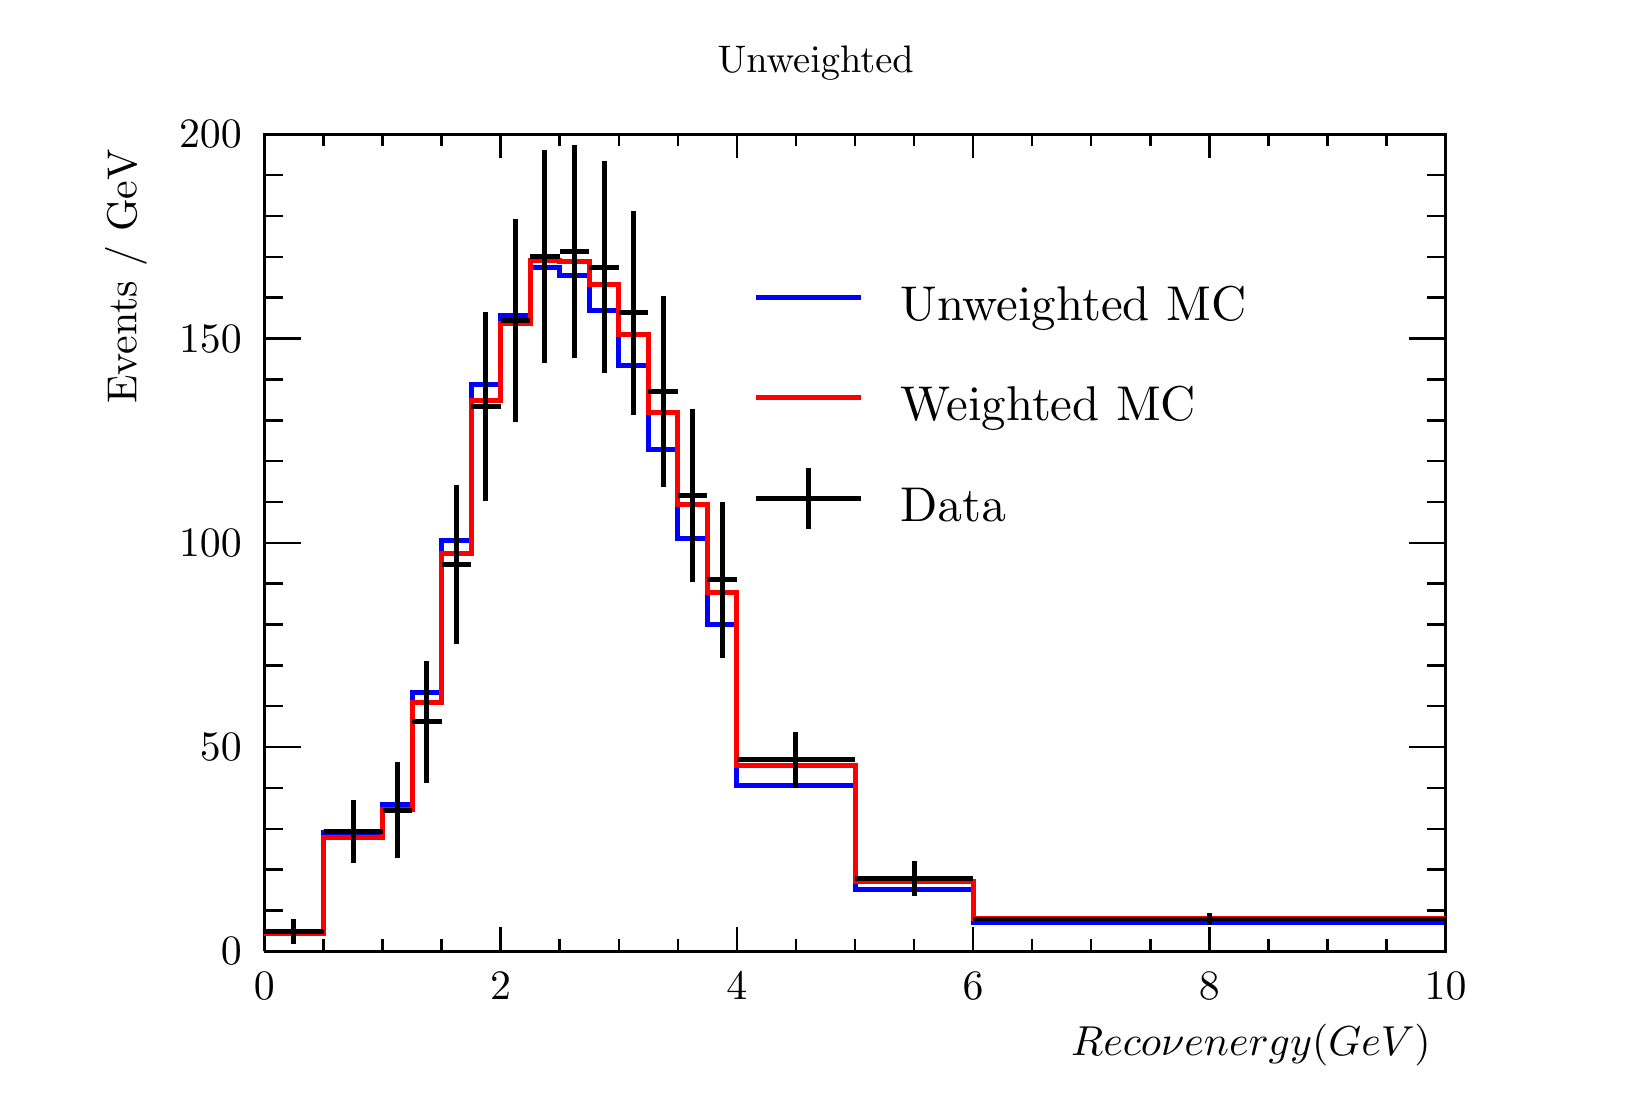
\begin{tikzpicture}
\pgfdeclareplotmark{cross} {
\pgfpathmoveto{\pgfpoint{-0.3\pgfplotmarksize}{\pgfplotmarksize}}
\pgfpathlineto{\pgfpoint{+0.3\pgfplotmarksize}{\pgfplotmarksize}}
\pgfpathlineto{\pgfpoint{+0.3\pgfplotmarksize}{0.3\pgfplotmarksize}}
\pgfpathlineto{\pgfpoint{+1\pgfplotmarksize}{0.3\pgfplotmarksize}}
\pgfpathlineto{\pgfpoint{+1\pgfplotmarksize}{-0.3\pgfplotmarksize}}
\pgfpathlineto{\pgfpoint{+0.3\pgfplotmarksize}{-0.3\pgfplotmarksize}}
\pgfpathlineto{\pgfpoint{+0.3\pgfplotmarksize}{-1.\pgfplotmarksize}}
\pgfpathlineto{\pgfpoint{-0.3\pgfplotmarksize}{-1.\pgfplotmarksize}}
\pgfpathlineto{\pgfpoint{-0.3\pgfplotmarksize}{-0.3\pgfplotmarksize}}
\pgfpathlineto{\pgfpoint{-1.\pgfplotmarksize}{-0.3\pgfplotmarksize}}
\pgfpathlineto{\pgfpoint{-1.\pgfplotmarksize}{0.3\pgfplotmarksize}}
\pgfpathlineto{\pgfpoint{-0.3\pgfplotmarksize}{0.3\pgfplotmarksize}}
\pgfpathclose
\pgfusepathqstroke
}
\pgfdeclareplotmark{cross*} {
\pgfpathmoveto{\pgfpoint{-0.3\pgfplotmarksize}{\pgfplotmarksize}}
\pgfpathlineto{\pgfpoint{+0.3\pgfplotmarksize}{\pgfplotmarksize}}
\pgfpathlineto{\pgfpoint{+0.3\pgfplotmarksize}{0.3\pgfplotmarksize}}
\pgfpathlineto{\pgfpoint{+1\pgfplotmarksize}{0.3\pgfplotmarksize}}
\pgfpathlineto{\pgfpoint{+1\pgfplotmarksize}{-0.3\pgfplotmarksize}}
\pgfpathlineto{\pgfpoint{+0.3\pgfplotmarksize}{-0.3\pgfplotmarksize}}
\pgfpathlineto{\pgfpoint{+0.3\pgfplotmarksize}{-1.\pgfplotmarksize}}
\pgfpathlineto{\pgfpoint{-0.3\pgfplotmarksize}{-1.\pgfplotmarksize}}
\pgfpathlineto{\pgfpoint{-0.3\pgfplotmarksize}{-0.3\pgfplotmarksize}}
\pgfpathlineto{\pgfpoint{-1.\pgfplotmarksize}{-0.3\pgfplotmarksize}}
\pgfpathlineto{\pgfpoint{-1.\pgfplotmarksize}{0.3\pgfplotmarksize}}
\pgfpathlineto{\pgfpoint{-0.3\pgfplotmarksize}{0.3\pgfplotmarksize}}
\pgfpathclose
\pgfusepathqfillstroke
}
\pgfdeclareplotmark{newstar} {
\pgfpathmoveto{\pgfqpoint{0pt}{\pgfplotmarksize}}
\pgfpathlineto{\pgfqpointpolar{44}{0.5\pgfplotmarksize}}
\pgfpathlineto{\pgfqpointpolar{18}{\pgfplotmarksize}}
\pgfpathlineto{\pgfqpointpolar{-20}{0.5\pgfplotmarksize}}
\pgfpathlineto{\pgfqpointpolar{-54}{\pgfplotmarksize}}
\pgfpathlineto{\pgfqpointpolar{-90}{0.5\pgfplotmarksize}}
\pgfpathlineto{\pgfqpointpolar{234}{\pgfplotmarksize}}
\pgfpathlineto{\pgfqpointpolar{198}{0.5\pgfplotmarksize}}
\pgfpathlineto{\pgfqpointpolar{162}{\pgfplotmarksize}}
\pgfpathlineto{\pgfqpointpolar{134}{0.5\pgfplotmarksize}}
\pgfpathclose
\pgfusepathqstroke
}
\pgfdeclareplotmark{newstar*} {
\pgfpathmoveto{\pgfqpoint{0pt}{\pgfplotmarksize}}
\pgfpathlineto{\pgfqpointpolar{44}{0.5\pgfplotmarksize}}
\pgfpathlineto{\pgfqpointpolar{18}{\pgfplotmarksize}}
\pgfpathlineto{\pgfqpointpolar{-20}{0.5\pgfplotmarksize}}
\pgfpathlineto{\pgfqpointpolar{-54}{\pgfplotmarksize}}
\pgfpathlineto{\pgfqpointpolar{-90}{0.5\pgfplotmarksize}}
\pgfpathlineto{\pgfqpointpolar{234}{\pgfplotmarksize}}
\pgfpathlineto{\pgfqpointpolar{198}{0.5\pgfplotmarksize}}
\pgfpathlineto{\pgfqpointpolar{162}{\pgfplotmarksize}}
\pgfpathlineto{\pgfqpointpolar{134}{0.5\pgfplotmarksize}}
\pgfpathclose
\pgfusepathqfillstroke
}
\definecolor{c}{rgb}{1,1,1};
\draw [color=c, fill=c] (0,0) rectangle (20,13.4752);
\draw [color=c, fill=c] (3,1.75177) rectangle (18,12.1277);
\definecolor{c}{rgb}{0,0,0};
\draw [c,line width=0.9] (3,1.75177) -- (3,12.1277) -- (18,12.1277) -- (18,1.75177) -- (3,1.75177);
\definecolor{c}{rgb}{1,1,1};
\draw [color=c, fill=c] (3,1.75177) rectangle (18,12.1277);
\definecolor{c}{rgb}{0,0,0};
\draw [c,line width=0.9] (3,1.75177) -- (3,12.1277) -- (18,12.1277) -- (18,1.75177) -- (3,1.75177);
\definecolor{c}{rgb}{0,0,1};
\draw [c,line width=1.8] (3,1.98647) -- (3.75,1.98647) -- (3.75,3.25573) -- (4.5,3.25573) -- (4.5,3.6191) -- (4.875,3.6191) -- (4.875,5.04048) -- (5.25,5.04048) -- (5.25,6.97323) -- (5.625,6.97323) -- (5.625,8.94826) -- (6,8.94826) -- (6,9.82879) --
 (6.375,9.82879) -- (6.375,10.4386) -- (6.75,10.4386) -- (6.75,10.3354) -- (7.125,10.3354) -- (7.125,9.89162) -- (7.5,9.89162) -- (7.5,9.19114) -- (7.875,9.19114) -- (7.875,8.12045) -- (8.25,8.12045) -- (8.25,6.99477) -- (8.625,6.99477) --
 (8.625,5.90293) -- (9,5.90293) -- (9,3.85844) -- (10.5,3.85844) -- (10.5,2.54063) -- (12,2.54063) -- (12,2.12032) -- (18,2.12032);
\definecolor{c}{rgb}{0,0,0};
\draw [c,line width=0.9] (3,1.75177) -- (18,1.75177);
\draw [c,line width=0.9] (3,2.05496) -- (3,1.75177);
\draw [c,line width=0.9] (3.75,1.90337) -- (3.75,1.75177);
\draw [c,line width=0.9] (4.5,1.90337) -- (4.5,1.75177);
\draw [c,line width=0.9] (5.25,1.90337) -- (5.25,1.75177);
\draw [c,line width=0.9] (6,2.05496) -- (6,1.75177);
\draw [c,line width=0.9] (6.75,1.90337) -- (6.75,1.75177);
\draw [c,line width=0.9] (7.5,1.90337) -- (7.5,1.75177);
\draw [c,line width=0.9] (8.25,1.90337) -- (8.25,1.75177);
\draw [c,line width=0.9] (9,2.05496) -- (9,1.75177);
\draw [c,line width=0.9] (9.75,1.90337) -- (9.75,1.75177);
\draw [c,line width=0.9] (10.5,1.90337) -- (10.5,1.75177);
\draw [c,line width=0.9] (11.25,1.90337) -- (11.25,1.75177);
\draw [c,line width=0.9] (12,2.05496) -- (12,1.75177);
\draw [c,line width=0.9] (12.75,1.90337) -- (12.75,1.75177);
\draw [c,line width=0.9] (13.5,1.90337) -- (13.5,1.75177);
\draw [c,line width=0.9] (14.25,1.90337) -- (14.25,1.75177);
\draw [c,line width=0.9] (15,2.05496) -- (15,1.75177);
\draw [c,line width=0.9] (15.75,1.90337) -- (15.75,1.75177);
\draw [c,line width=0.9] (16.5,1.90337) -- (16.5,1.75177);
\draw [c,line width=0.9] (17.25,1.90337) -- (17.25,1.75177);
\draw [c,line width=0.9] (18,2.05496) -- (18,1.75177);
\draw [anchor=base] (3,1.14539) node[scale=1.51215, color=c, rotate=0]{0};
\draw [anchor=base] (6,1.14539) node[scale=1.51215, color=c, rotate=0]{2};
\draw [anchor=base] (9,1.14539) node[scale=1.51215, color=c, rotate=0]{4};
\draw [anchor=base] (12,1.14539) node[scale=1.51215, color=c, rotate=0]{6};
\draw [anchor=base] (15,1.14539) node[scale=1.51215, color=c, rotate=0]{8};
\draw [anchor=base] (18,1.14539) node[scale=1.51215, color=c, rotate=0]{10};
\draw [anchor= east] (18,0.565957) node[scale=1.51215, color=c, rotate=0]{$Reco \nu energy (GeV)$};
\draw [c,line width=0.9] (3,12.1277) -- (18,12.1277);
\draw [c,line width=0.9] (3,11.8245) -- (3,12.1277);
\draw [c,line width=0.9] (3.75,11.9761) -- (3.75,12.1277);
\draw [c,line width=0.9] (4.5,11.9761) -- (4.5,12.1277);
\draw [c,line width=0.9] (5.25,11.9761) -- (5.25,12.1277);
\draw [c,line width=0.9] (6,11.8245) -- (6,12.1277);
\draw [c,line width=0.9] (6.75,11.9761) -- (6.75,12.1277);
\draw [c,line width=0.9] (7.5,11.9761) -- (7.5,12.1277);
\draw [c,line width=0.9] (8.25,11.9761) -- (8.25,12.1277);
\draw [c,line width=0.9] (9,11.8245) -- (9,12.1277);
\draw [c,line width=0.9] (9.75,11.9761) -- (9.75,12.1277);
\draw [c,line width=0.9] (10.5,11.9761) -- (10.5,12.1277);
\draw [c,line width=0.9] (11.25,11.9761) -- (11.25,12.1277);
\draw [c,line width=0.9] (12,11.8245) -- (12,12.1277);
\draw [c,line width=0.9] (12.75,11.9761) -- (12.75,12.1277);
\draw [c,line width=0.9] (13.5,11.9761) -- (13.5,12.1277);
\draw [c,line width=0.9] (14.25,11.9761) -- (14.25,12.1277);
\draw [c,line width=0.9] (15,11.8245) -- (15,12.1277);
\draw [c,line width=0.9] (15.75,11.9761) -- (15.75,12.1277);
\draw [c,line width=0.9] (16.5,11.9761) -- (16.5,12.1277);
\draw [c,line width=0.9] (17.25,11.9761) -- (17.25,12.1277);
\draw [c,line width=0.9] (18,11.8245) -- (18,12.1277);
\draw [c,line width=0.9] (3,1.75177) -- (3,12.1277);
\draw [c,line width=0.9] (3.462,1.75177) -- (3,1.75177);
\draw [c,line width=0.9] (3.231,2.27057) -- (3,2.27057);
\draw [c,line width=0.9] (3.231,2.78936) -- (3,2.78936);
\draw [c,line width=0.9] (3.231,3.30816) -- (3,3.30816);
\draw [c,line width=0.9] (3.231,3.82695) -- (3,3.82695);
\draw [c,line width=0.9] (3.462,4.34574) -- (3,4.34574);
\draw [c,line width=0.9] (3.231,4.86454) -- (3,4.86454);
\draw [c,line width=0.9] (3.231,5.38333) -- (3,5.38333);
\draw [c,line width=0.9] (3.231,5.90213) -- (3,5.90213);
\draw [c,line width=0.9] (3.231,6.42092) -- (3,6.42092);
\draw [c,line width=0.9] (3.462,6.93972) -- (3,6.93972);
\draw [c,line width=0.9] (3.231,7.45851) -- (3,7.45851);
\draw [c,line width=0.9] (3.231,7.97731) -- (3,7.97731);
\draw [c,line width=0.9] (3.231,8.4961) -- (3,8.4961);
\draw [c,line width=0.9] (3.231,9.01489) -- (3,9.01489);
\draw [c,line width=0.9] (3.462,9.53369) -- (3,9.53369);
\draw [c,line width=0.9] (3.231,10.0525) -- (3,10.0525);
\draw [c,line width=0.9] (3.231,10.5713) -- (3,10.5713);
\draw [c,line width=0.9] (3.231,11.0901) -- (3,11.0901);
\draw [c,line width=0.9] (3.231,11.6089) -- (3,11.6089);
\draw [c,line width=0.9] (3.462,12.1277) -- (3,12.1277);
\draw [anchor= east] (2.9,1.75177) node[scale=1.51215, color=c, rotate=0]{0};
\draw [anchor= east] (2.9,4.34574) node[scale=1.51215, color=c, rotate=0]{50};
\draw [anchor= east] (2.9,6.93972) node[scale=1.51215, color=c, rotate=0]{100};
\draw [anchor= east] (2.9,9.53369) node[scale=1.51215, color=c, rotate=0]{150};
\draw [anchor= east] (2.9,12.1277) node[scale=1.51215, color=c, rotate=0]{200};
\draw [anchor= east] (1.24,12.1277) node[scale=1.51215, color=c, rotate=90]{Events / GeV};
\draw [c,line width=0.9] (18,1.75177) -- (18,12.1277);
\draw [c,line width=0.9] (17.538,1.75177) -- (18,1.75177);
\draw [c,line width=0.9] (17.769,2.27057) -- (18,2.27057);
\draw [c,line width=0.9] (17.769,2.78936) -- (18,2.78936);
\draw [c,line width=0.9] (17.769,3.30816) -- (18,3.30816);
\draw [c,line width=0.9] (17.769,3.82695) -- (18,3.82695);
\draw [c,line width=0.9] (17.538,4.34574) -- (18,4.34574);
\draw [c,line width=0.9] (17.769,4.86454) -- (18,4.86454);
\draw [c,line width=0.9] (17.769,5.38333) -- (18,5.38333);
\draw [c,line width=0.9] (17.769,5.90213) -- (18,5.90213);
\draw [c,line width=0.9] (17.769,6.42092) -- (18,6.42092);
\draw [c,line width=0.9] (17.538,6.93972) -- (18,6.93972);
\draw [c,line width=0.9] (17.769,7.45851) -- (18,7.45851);
\draw [c,line width=0.9] (17.769,7.97731) -- (18,7.97731);
\draw [c,line width=0.9] (17.769,8.4961) -- (18,8.4961);
\draw [c,line width=0.9] (17.769,9.01489) -- (18,9.01489);
\draw [c,line width=0.9] (17.538,9.53369) -- (18,9.53369);
\draw [c,line width=0.9] (17.769,10.0525) -- (18,10.0525);
\draw [c,line width=0.9] (17.769,10.5713) -- (18,10.5713);
\draw [c,line width=0.9] (17.769,11.0901) -- (18,11.0901);
\draw [c,line width=0.9] (17.769,11.6089) -- (18,11.6089);
\draw [c,line width=0.9] (17.538,12.1277) -- (18,12.1277);
\definecolor{c}{rgb}{1,1,1};
\draw [color=c, fill=c] (2,12.6667) rectangle (18,13.4078);
\definecolor{c}{rgb}{0,0,0};
\draw (10,13.0372) node[scale=1.38614, color=c, rotate=0]{Unweighted};
\definecolor{c}{rgb}{1,0,0};
\draw [c,line width=1.8] (3,1.97488) -- (3.75,1.97488) -- (3.75,3.19245) -- (4.5,3.19245) -- (4.5,3.55386) -- (4.875,3.55386) -- (4.875,4.91444) -- (5.25,4.91444) -- (5.25,6.79985) -- (5.625,6.79985) -- (5.625,8.75122) -- (6,8.75122) -- (6,9.72631)
 -- (6.375,9.72631) -- (6.375,10.5298) -- (6.75,10.5298) -- (6.75,10.5147) -- (7.125,10.5147) -- (7.125,10.2266) -- (7.5,10.2266) -- (7.5,9.5831) -- (7.875,9.5831) -- (7.875,8.59225) -- (8.25,8.59225) -- (8.25,7.42656) -- (8.625,7.42656) --
 (8.625,6.31278) -- (9,6.31278) -- (9,4.11723) -- (10.5,4.11723) -- (10.5,2.63867) -- (12,2.63867) -- (12,2.16701) -- (18,2.16701);
\definecolor{c}{rgb}{0,0,0};
\draw [c,line width=1.8] (3.375,1.84066) -- (3.375,2.00169);
\draw [c,line width=1.8] (3.375,2.00169) -- (3.375,2.16272);
\draw [c,line width=1.8] (3,2.00169) -- (3.375,2.00169);
\draw [c,line width=1.8] (3.375,2.00169) -- (3.75,2.00169);
\foreach \P in {(3.375,2.00169)}{\draw[mark options={color=c,fill=c},mark size=2.402402pt, line width=0.000000pt, mark=*,mark size=1pt] plot coordinates {\P};}
\draw [c,line width=1.8] (4.125,2.87965) -- (4.125,3.27753);
\draw [c,line width=1.8] (4.125,3.27753) -- (4.125,3.67542);
\draw [c,line width=1.8] (3.75,3.27753) -- (4.125,3.27753);
\draw [c,line width=1.8] (4.125,3.27753) -- (4.5,3.27753);
\foreach \P in {(4.125,3.27753)}{\draw[mark options={color=c,fill=c},mark size=2.402402pt, line width=0.000000pt, mark=*,mark size=1pt] plot coordinates {\P};}
\draw [c,line width=1.8] (4.6875,2.93271) -- (4.6875,3.54227);
\draw [c,line width=1.8] (4.6875,3.54227) -- (4.6875,4.15183);
\draw [c,line width=1.8] (4.5,3.54227) -- (4.6875,3.54227);
\draw [c,line width=1.8] (4.6875,3.54227) -- (4.875,3.54227);
\foreach \P in {(4.6875,3.54227)}{\draw[mark options={color=c,fill=c},mark size=2.402402pt, line width=0.000000pt, mark=*,mark size=1pt] plot coordinates {\P};}
\draw [c,line width=1.8] (5.0625,3.88772) -- (5.0625,4.66529);
\draw [c,line width=1.8] (5.0625,4.66529) -- (5.0625,5.44285);
\draw [c,line width=1.8] (4.875,4.66529) -- (5.0625,4.66529);
\draw [c,line width=1.8] (5.0625,4.66529) -- (5.25,4.66529);
\foreach \P in {(5.0625,4.66529)}{\draw[mark options={color=c,fill=c},mark size=2.402402pt, line width=0.000000pt, mark=*,mark size=1pt] plot coordinates {\P};}
\draw [c,line width=1.8] (5.4375,5.6565) -- (5.4375,6.66638);
\draw [c,line width=1.8] (5.4375,6.66638) -- (5.4375,7.67627);
\draw [c,line width=1.8] (5.25,6.66638) -- (5.4375,6.66638);
\draw [c,line width=1.8] (5.4375,6.66638) -- (5.625,6.66638);
\foreach \P in {(5.4375,6.66638)}{\draw[mark options={color=c,fill=c},mark size=2.402402pt, line width=0.000000pt, mark=*,mark size=1pt] plot coordinates {\P};}
\draw [c,line width=1.8] (5.8125,7.47154) -- (5.8125,8.6697);
\draw [c,line width=1.8] (5.8125,8.6697) -- (5.8125,9.86786);
\draw [c,line width=1.8] (5.625,8.6697) -- (5.8125,8.6697);
\draw [c,line width=1.8] (5.8125,8.6697) -- (6,8.6697);
\foreach \P in {(5.8125,8.6697)}{\draw[mark options={color=c,fill=c},mark size=2.402402pt, line width=0.000000pt, mark=*,mark size=1pt] plot coordinates {\P};}
\draw [c,line width=1.8] (6.1875,8.46951) -- (6.1875,9.75852);
\draw [c,line width=1.8] (6.1875,9.75852) -- (6.1875,11.0475);
\draw [c,line width=1.8] (6,9.75852) -- (6.1875,9.75852);
\draw [c,line width=1.8] (6.1875,9.75852) -- (6.375,9.75852);
\foreach \P in {(6.1875,9.75852)}{\draw[mark options={color=c,fill=c},mark size=2.402402pt, line width=0.000000pt, mark=*,mark size=1pt] plot coordinates {\P};}
\draw [c,line width=1.8] (6.5625,9.22153) -- (6.5625,10.5746);
\draw [c,line width=1.8] (6.5625,10.5746) -- (6.5625,11.9277);
\draw [c,line width=1.8] (6.375,10.5746) -- (6.5625,10.5746);
\draw [c,line width=1.8] (6.5625,10.5746) -- (6.75,10.5746);
\foreach \P in {(6.5625,10.5746)}{\draw[mark options={color=c,fill=c},mark size=2.402402pt, line width=0.000000pt, mark=*,mark size=1pt] plot coordinates {\P};}
\draw [c,line width=1.8] (6.9375,9.28066) -- (6.9375,10.6387);
\draw [c,line width=1.8] (6.9375,10.6387) -- (6.9375,11.9967);
\draw [c,line width=1.8] (6.75,10.6387) -- (6.9375,10.6387);
\draw [c,line width=1.8] (6.9375,10.6387) -- (7.125,10.6387);
\foreach \P in {(6.9375,10.6387)}{\draw[mark options={color=c,fill=c},mark size=2.402402pt, line width=0.000000pt, mark=*,mark size=1pt] plot coordinates {\P};}
\draw [c,line width=1.8] (7.3125,9.09923) -- (7.3125,10.4421);
\draw [c,line width=1.8] (7.3125,10.4421) -- (7.3125,11.7851);
\draw [c,line width=1.8] (7.125,10.4421) -- (7.3125,10.4421);
\draw [c,line width=1.8] (7.3125,10.4421) -- (7.5,10.4421);
\foreach \P in {(7.3125,10.4421)}{\draw[mark options={color=c,fill=c},mark size=2.402402pt, line width=0.000000pt, mark=*,mark size=1pt] plot coordinates {\P};}
\draw [c,line width=1.8] (7.6875,8.56395) -- (7.6875,9.8612);
\draw [c,line width=1.8] (7.6875,9.8612) -- (7.6875,11.1584);
\draw [c,line width=1.8] (7.5,9.8612) -- (7.6875,9.8612);
\draw [c,line width=1.8] (7.6875,9.8612) -- (7.875,9.8612);
\foreach \P in {(7.6875,9.8612)}{\draw[mark options={color=c,fill=c},mark size=2.402402pt, line width=0.000000pt, mark=*,mark size=1pt] plot coordinates {\P};}
\draw [c,line width=1.8] (8.0625,7.64809) -- (8.0625,8.86286);
\draw [c,line width=1.8] (8.0625,8.86286) -- (8.0625,10.0776);
\draw [c,line width=1.8] (7.875,8.86286) -- (8.0625,8.86286);
\draw [c,line width=1.8] (8.0625,8.86286) -- (8.25,8.86286);
\foreach \P in {(8.0625,8.86286)}{\draw[mark options={color=c,fill=c},mark size=2.402402pt, line width=0.000000pt, mark=*,mark size=1pt] plot coordinates {\P};}
\draw [c,line width=1.8] (8.4375,6.44341) -- (8.4375,7.53932);
\draw [c,line width=1.8] (8.4375,7.53932) -- (8.4375,8.63524);
\draw [c,line width=1.8] (8.25,7.53932) -- (8.4375,7.53932);
\draw [c,line width=1.8] (8.4375,7.53932) -- (8.625,7.53932);
\foreach \P in {(8.4375,7.53932)}{\draw[mark options={color=c,fill=c},mark size=2.402402pt, line width=0.000000pt, mark=*,mark size=1pt] plot coordinates {\P};}
\draw [c,line width=1.8] (8.8125,5.48327) -- (8.8125,6.47309);
\draw [c,line width=1.8] (8.8125,6.47309) -- (8.8125,7.46292);
\draw [c,line width=1.8] (8.625,6.47309) -- (8.8125,6.47309);
\draw [c,line width=1.8] (8.8125,6.47309) -- (9,6.47309);
\foreach \P in {(8.8125,6.47309)}{\draw[mark options={color=c,fill=c},mark size=2.402402pt, line width=0.000000pt, mark=*,mark size=1pt] plot coordinates {\P};}
\draw [c,line width=1.8] (9.75,3.83199) -- (9.75,4.18746);
\draw [c,line width=1.8] (9.75,4.18746) -- (9.75,4.54294);
\draw [c,line width=1.8] (9,4.18746) -- (9.75,4.18746);
\draw [c,line width=1.8] (9.75,4.18746) -- (10.5,4.18746);
\foreach \P in {(9.75,4.18746)}{\draw[mark options={color=c,fill=c},mark size=2.402402pt, line width=0.000000pt, mark=*,mark size=1pt] plot coordinates {\P};}
\draw [c,line width=1.8] (11.25,2.45978) -- (11.25,2.67912);
\draw [c,line width=1.8] (11.25,2.67912) -- (11.25,2.89846);
\draw [c,line width=1.8] (10.5,2.67912) -- (11.25,2.67912);
\draw [c,line width=1.8] (11.25,2.67912) -- (12,2.67912);
\foreach \P in {(11.25,2.67912)}{\draw[mark options={color=c,fill=c},mark size=2.402402pt, line width=0.000000pt, mark=*,mark size=1pt] plot coordinates {\P};}
\draw [c,line width=1.8] (15,2.08929) -- (15,2.16226);
\draw [c,line width=1.8] (15,2.16226) -- (15,2.23523);
\draw [c,line width=1.8] (12,2.16226) -- (15,2.16226);
\draw [c,line width=1.8] (15,2.16226) -- (18,2.16226);
\foreach \P in {(15,2.16226)}{\draw[mark options={color=c,fill=c},mark size=2.402402pt, line width=0.000000pt, mark=*,mark size=1pt] plot coordinates {\P};}
\draw [c,line width=1.8] (3.375,1.84066) -- (3.375,2.00169);
\draw [c,line width=1.8] (3.375,2.00169) -- (3.375,2.16272);
\draw [c,line width=1.8] (3,2.00169) -- (3.375,2.00169);
\draw [c,line width=1.8] (3.375,2.00169) -- (3.75,2.00169);
\foreach \P in {(3.375,2.00169)}{\draw[mark options={color=c,fill=c},mark size=2.402402pt, line width=0.000000pt, mark=*,mark size=1pt] plot coordinates {\P};}
\draw [c,line width=1.8] (4.125,2.87965) -- (4.125,3.27753);
\draw [c,line width=1.8] (4.125,3.27753) -- (4.125,3.67542);
\draw [c,line width=1.8] (3.75,3.27753) -- (4.125,3.27753);
\draw [c,line width=1.8] (4.125,3.27753) -- (4.5,3.27753);
\foreach \P in {(4.125,3.27753)}{\draw[mark options={color=c,fill=c},mark size=2.402402pt, line width=0.000000pt, mark=*,mark size=1pt] plot coordinates {\P};}
\draw [c,line width=1.8] (4.6875,2.93271) -- (4.6875,3.54227);
\draw [c,line width=1.8] (4.6875,3.54227) -- (4.6875,4.15183);
\draw [c,line width=1.8] (4.5,3.54227) -- (4.6875,3.54227);
\draw [c,line width=1.8] (4.6875,3.54227) -- (4.875,3.54227);
\foreach \P in {(4.6875,3.54227)}{\draw[mark options={color=c,fill=c},mark size=2.402402pt, line width=0.000000pt, mark=*,mark size=1pt] plot coordinates {\P};}
\draw [c,line width=1.8] (5.0625,3.88772) -- (5.0625,4.66529);
\draw [c,line width=1.8] (5.0625,4.66529) -- (5.0625,5.44285);
\draw [c,line width=1.8] (4.875,4.66529) -- (5.0625,4.66529);
\draw [c,line width=1.8] (5.0625,4.66529) -- (5.25,4.66529);
\foreach \P in {(5.0625,4.66529)}{\draw[mark options={color=c,fill=c},mark size=2.402402pt, line width=0.000000pt, mark=*,mark size=1pt] plot coordinates {\P};}
\draw [c,line width=1.8] (5.4375,5.6565) -- (5.4375,6.66638);
\draw [c,line width=1.8] (5.4375,6.66638) -- (5.4375,7.67627);
\draw [c,line width=1.8] (5.25,6.66638) -- (5.4375,6.66638);
\draw [c,line width=1.8] (5.4375,6.66638) -- (5.625,6.66638);
\foreach \P in {(5.4375,6.66638)}{\draw[mark options={color=c,fill=c},mark size=2.402402pt, line width=0.000000pt, mark=*,mark size=1pt] plot coordinates {\P};}
\draw [c,line width=1.8] (5.8125,7.47154) -- (5.8125,8.6697);
\draw [c,line width=1.8] (5.8125,8.6697) -- (5.8125,9.86786);
\draw [c,line width=1.8] (5.625,8.6697) -- (5.8125,8.6697);
\draw [c,line width=1.8] (5.8125,8.6697) -- (6,8.6697);
\foreach \P in {(5.8125,8.6697)}{\draw[mark options={color=c,fill=c},mark size=2.402402pt, line width=0.000000pt, mark=*,mark size=1pt] plot coordinates {\P};}
\draw [c,line width=1.8] (6.1875,8.46951) -- (6.1875,9.75852);
\draw [c,line width=1.8] (6.1875,9.75852) -- (6.1875,11.0475);
\draw [c,line width=1.8] (6,9.75852) -- (6.1875,9.75852);
\draw [c,line width=1.8] (6.1875,9.75852) -- (6.375,9.75852);
\foreach \P in {(6.1875,9.75852)}{\draw[mark options={color=c,fill=c},mark size=2.402402pt, line width=0.000000pt, mark=*,mark size=1pt] plot coordinates {\P};}
\draw [c,line width=1.8] (6.5625,9.22153) -- (6.5625,10.5746);
\draw [c,line width=1.8] (6.5625,10.5746) -- (6.5625,11.9277);
\draw [c,line width=1.8] (6.375,10.5746) -- (6.5625,10.5746);
\draw [c,line width=1.8] (6.5625,10.5746) -- (6.75,10.5746);
\foreach \P in {(6.5625,10.5746)}{\draw[mark options={color=c,fill=c},mark size=2.402402pt, line width=0.000000pt, mark=*,mark size=1pt] plot coordinates {\P};}
\draw [c,line width=1.8] (6.9375,9.28066) -- (6.9375,10.6387);
\draw [c,line width=1.8] (6.9375,10.6387) -- (6.9375,11.9967);
\draw [c,line width=1.8] (6.75,10.6387) -- (6.9375,10.6387);
\draw [c,line width=1.8] (6.9375,10.6387) -- (7.125,10.6387);
\foreach \P in {(6.9375,10.6387)}{\draw[mark options={color=c,fill=c},mark size=2.402402pt, line width=0.000000pt, mark=*,mark size=1pt] plot coordinates {\P};}
\draw [c,line width=1.8] (7.3125,9.09923) -- (7.3125,10.4421);
\draw [c,line width=1.8] (7.3125,10.4421) -- (7.3125,11.7851);
\draw [c,line width=1.8] (7.125,10.4421) -- (7.3125,10.4421);
\draw [c,line width=1.8] (7.3125,10.4421) -- (7.5,10.4421);
\foreach \P in {(7.3125,10.4421)}{\draw[mark options={color=c,fill=c},mark size=2.402402pt, line width=0.000000pt, mark=*,mark size=1pt] plot coordinates {\P};}
\draw [c,line width=1.8] (7.6875,8.56395) -- (7.6875,9.8612);
\draw [c,line width=1.8] (7.6875,9.8612) -- (7.6875,11.1584);
\draw [c,line width=1.8] (7.5,9.8612) -- (7.6875,9.8612);
\draw [c,line width=1.8] (7.6875,9.8612) -- (7.875,9.8612);
\foreach \P in {(7.6875,9.8612)}{\draw[mark options={color=c,fill=c},mark size=2.402402pt, line width=0.000000pt, mark=*,mark size=1pt] plot coordinates {\P};}
\draw [c,line width=1.8] (8.0625,7.64809) -- (8.0625,8.86286);
\draw [c,line width=1.8] (8.0625,8.86286) -- (8.0625,10.0776);
\draw [c,line width=1.8] (7.875,8.86286) -- (8.0625,8.86286);
\draw [c,line width=1.8] (8.0625,8.86286) -- (8.25,8.86286);
\foreach \P in {(8.0625,8.86286)}{\draw[mark options={color=c,fill=c},mark size=2.402402pt, line width=0.000000pt, mark=*,mark size=1pt] plot coordinates {\P};}
\draw [c,line width=1.8] (8.4375,6.44341) -- (8.4375,7.53932);
\draw [c,line width=1.8] (8.4375,7.53932) -- (8.4375,8.63524);
\draw [c,line width=1.8] (8.25,7.53932) -- (8.4375,7.53932);
\draw [c,line width=1.8] (8.4375,7.53932) -- (8.625,7.53932);
\foreach \P in {(8.4375,7.53932)}{\draw[mark options={color=c,fill=c},mark size=2.402402pt, line width=0.000000pt, mark=*,mark size=1pt] plot coordinates {\P};}
\draw [c,line width=1.8] (8.8125,5.48327) -- (8.8125,6.47309);
\draw [c,line width=1.8] (8.8125,6.47309) -- (8.8125,7.46292);
\draw [c,line width=1.8] (8.625,6.47309) -- (8.8125,6.47309);
\draw [c,line width=1.8] (8.8125,6.47309) -- (9,6.47309);
\foreach \P in {(8.8125,6.47309)}{\draw[mark options={color=c,fill=c},mark size=2.402402pt, line width=0.000000pt, mark=*,mark size=1pt] plot coordinates {\P};}
\draw [c,line width=1.8] (9.75,3.83199) -- (9.75,4.18746);
\draw [c,line width=1.8] (9.75,4.18746) -- (9.75,4.54294);
\draw [c,line width=1.8] (9,4.18746) -- (9.75,4.18746);
\draw [c,line width=1.8] (9.75,4.18746) -- (10.5,4.18746);
\foreach \P in {(9.75,4.18746)}{\draw[mark options={color=c,fill=c},mark size=2.402402pt, line width=0.000000pt, mark=*,mark size=1pt] plot coordinates {\P};}
\draw [c,line width=1.8] (11.25,2.45978) -- (11.25,2.67912);
\draw [c,line width=1.8] (11.25,2.67912) -- (11.25,2.89846);
\draw [c,line width=1.8] (10.5,2.67912) -- (11.25,2.67912);
\draw [c,line width=1.8] (11.25,2.67912) -- (12,2.67912);
\foreach \P in {(11.25,2.67912)}{\draw[mark options={color=c,fill=c},mark size=2.402402pt, line width=0.000000pt, mark=*,mark size=1pt] plot coordinates {\P};}
\draw [c,line width=1.8] (15,2.08929) -- (15,2.16226);
\draw [c,line width=1.8] (15,2.16226) -- (15,2.23523);
\draw [c,line width=1.8] (12,2.16226) -- (15,2.16226);
\draw [c,line width=1.8] (15,2.16226) -- (18,2.16226);
\foreach \P in {(15,2.16226)}{\draw[mark options={color=c,fill=c},mark size=2.402402pt, line width=0.000000pt, mark=*,mark size=1pt] plot coordinates {\P};}
\definecolor{c}{rgb}{1,1,1};
\draw [color=c, fill=c] (8.96454,6.86525) rectangle (16.539,10.695);
\definecolor{c}{rgb}{0,0,0};
\draw [anchor=base west] (10.8582,9.7695) node[scale=1.76417, color=c, rotate=0]{Unweighted MC};
\definecolor{c}{rgb}{0,0,1};
\draw [c,line width=1.8] (9.24858,10.0567) -- (10.5741,10.0567);
\definecolor{c}{rgb}{0,0,0};
\draw [anchor=base west] (10.8582,8.49291) node[scale=1.76417, color=c, rotate=0]{Weighted MC};
\definecolor{c}{rgb}{1,0,0};
\draw [c,line width=1.8] (9.24858,8.78014) -- (10.5741,8.78014);
\definecolor{c}{rgb}{0,0,0};
\draw [anchor=base west] (10.8582,7.21631) node[scale=1.76417, color=c, rotate=0]{Data};
\draw [c,line width=1.8] (9.24858,7.50355) -- (10.5741,7.50355);
\draw [c,line width=1.8] (9.91135,7.12057) -- (9.91135,7.88653);
\end{tikzpicture}

		\end{adjustbox}
		\caption{FHC \nue}
	\end{subfigure} \\
	\begin{subfigure}[t]{.5\linewidth}
		\begin{adjustbox}{max totalsize=\linewidth, center}
			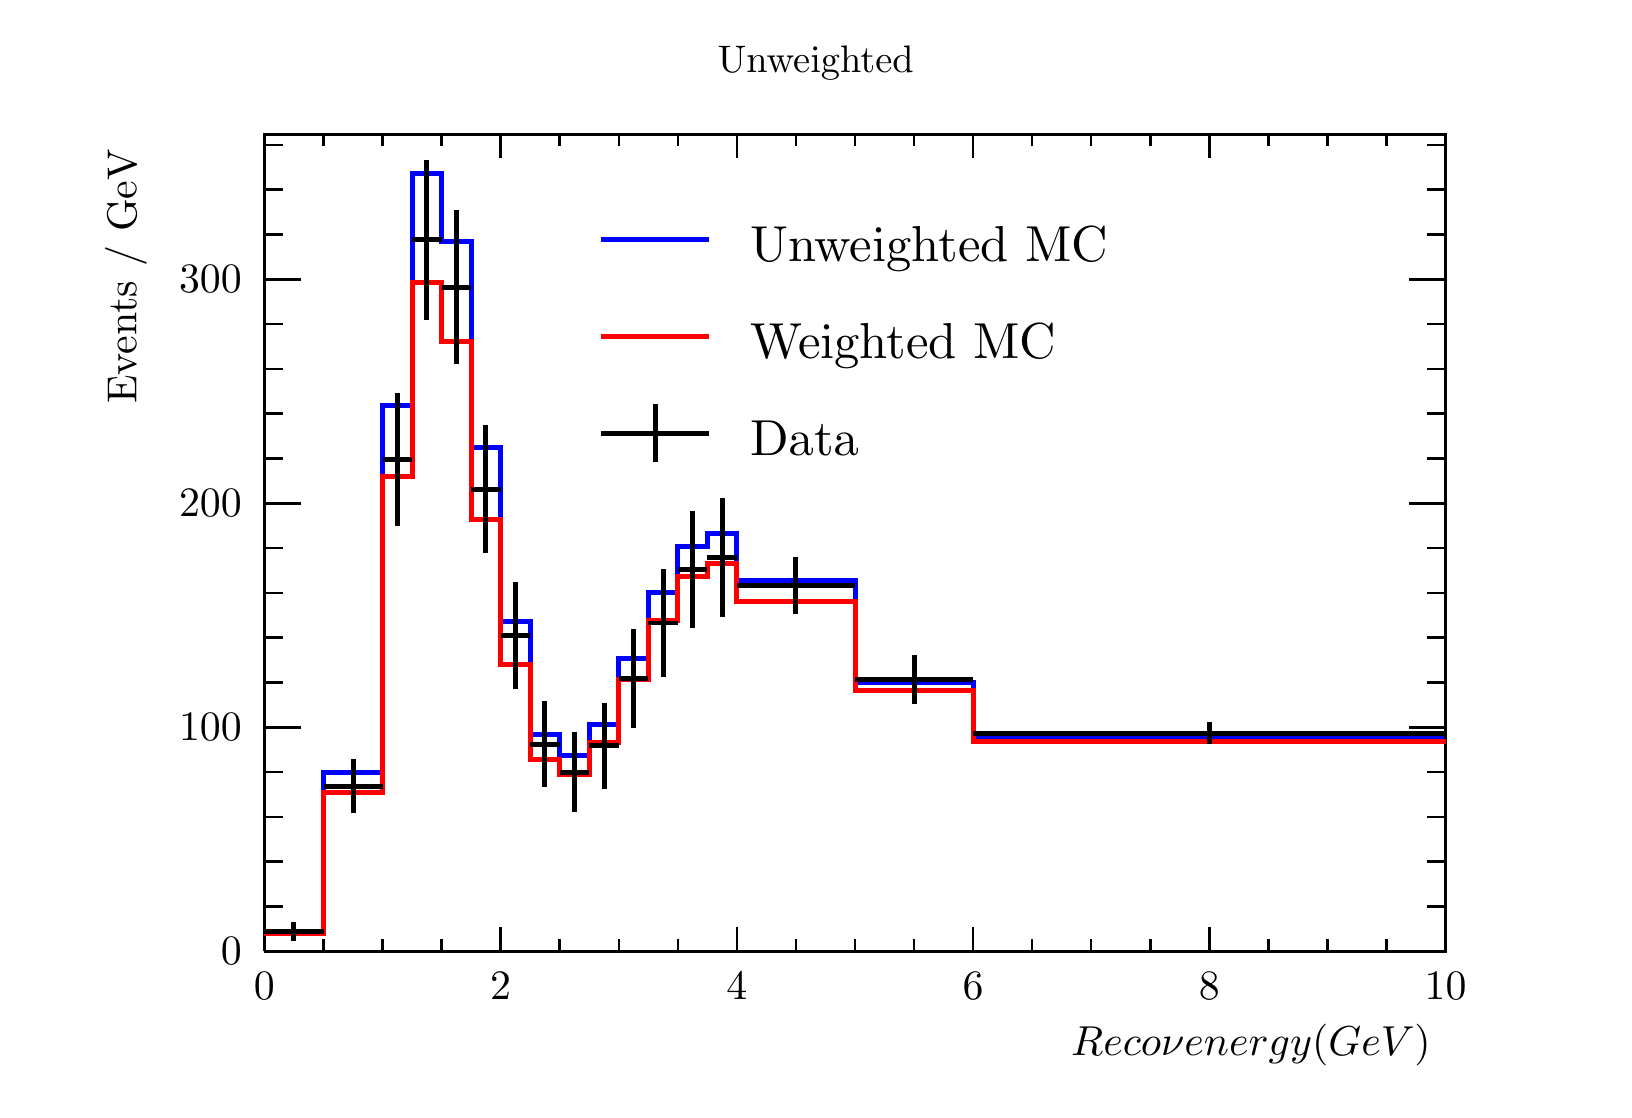
\begin{tikzpicture}
\pgfdeclareplotmark{cross} {
\pgfpathmoveto{\pgfpoint{-0.3\pgfplotmarksize}{\pgfplotmarksize}}
\pgfpathlineto{\pgfpoint{+0.3\pgfplotmarksize}{\pgfplotmarksize}}
\pgfpathlineto{\pgfpoint{+0.3\pgfplotmarksize}{0.3\pgfplotmarksize}}
\pgfpathlineto{\pgfpoint{+1\pgfplotmarksize}{0.3\pgfplotmarksize}}
\pgfpathlineto{\pgfpoint{+1\pgfplotmarksize}{-0.3\pgfplotmarksize}}
\pgfpathlineto{\pgfpoint{+0.3\pgfplotmarksize}{-0.3\pgfplotmarksize}}
\pgfpathlineto{\pgfpoint{+0.3\pgfplotmarksize}{-1.\pgfplotmarksize}}
\pgfpathlineto{\pgfpoint{-0.3\pgfplotmarksize}{-1.\pgfplotmarksize}}
\pgfpathlineto{\pgfpoint{-0.3\pgfplotmarksize}{-0.3\pgfplotmarksize}}
\pgfpathlineto{\pgfpoint{-1.\pgfplotmarksize}{-0.3\pgfplotmarksize}}
\pgfpathlineto{\pgfpoint{-1.\pgfplotmarksize}{0.3\pgfplotmarksize}}
\pgfpathlineto{\pgfpoint{-0.3\pgfplotmarksize}{0.3\pgfplotmarksize}}
\pgfpathclose
\pgfusepathqstroke
}
\pgfdeclareplotmark{cross*} {
\pgfpathmoveto{\pgfpoint{-0.3\pgfplotmarksize}{\pgfplotmarksize}}
\pgfpathlineto{\pgfpoint{+0.3\pgfplotmarksize}{\pgfplotmarksize}}
\pgfpathlineto{\pgfpoint{+0.3\pgfplotmarksize}{0.3\pgfplotmarksize}}
\pgfpathlineto{\pgfpoint{+1\pgfplotmarksize}{0.3\pgfplotmarksize}}
\pgfpathlineto{\pgfpoint{+1\pgfplotmarksize}{-0.3\pgfplotmarksize}}
\pgfpathlineto{\pgfpoint{+0.3\pgfplotmarksize}{-0.3\pgfplotmarksize}}
\pgfpathlineto{\pgfpoint{+0.3\pgfplotmarksize}{-1.\pgfplotmarksize}}
\pgfpathlineto{\pgfpoint{-0.3\pgfplotmarksize}{-1.\pgfplotmarksize}}
\pgfpathlineto{\pgfpoint{-0.3\pgfplotmarksize}{-0.3\pgfplotmarksize}}
\pgfpathlineto{\pgfpoint{-1.\pgfplotmarksize}{-0.3\pgfplotmarksize}}
\pgfpathlineto{\pgfpoint{-1.\pgfplotmarksize}{0.3\pgfplotmarksize}}
\pgfpathlineto{\pgfpoint{-0.3\pgfplotmarksize}{0.3\pgfplotmarksize}}
\pgfpathclose
\pgfusepathqfillstroke
}
\pgfdeclareplotmark{newstar} {
\pgfpathmoveto{\pgfqpoint{0pt}{\pgfplotmarksize}}
\pgfpathlineto{\pgfqpointpolar{44}{0.5\pgfplotmarksize}}
\pgfpathlineto{\pgfqpointpolar{18}{\pgfplotmarksize}}
\pgfpathlineto{\pgfqpointpolar{-20}{0.5\pgfplotmarksize}}
\pgfpathlineto{\pgfqpointpolar{-54}{\pgfplotmarksize}}
\pgfpathlineto{\pgfqpointpolar{-90}{0.5\pgfplotmarksize}}
\pgfpathlineto{\pgfqpointpolar{234}{\pgfplotmarksize}}
\pgfpathlineto{\pgfqpointpolar{198}{0.5\pgfplotmarksize}}
\pgfpathlineto{\pgfqpointpolar{162}{\pgfplotmarksize}}
\pgfpathlineto{\pgfqpointpolar{134}{0.5\pgfplotmarksize}}
\pgfpathclose
\pgfusepathqstroke
}
\pgfdeclareplotmark{newstar*} {
\pgfpathmoveto{\pgfqpoint{0pt}{\pgfplotmarksize}}
\pgfpathlineto{\pgfqpointpolar{44}{0.5\pgfplotmarksize}}
\pgfpathlineto{\pgfqpointpolar{18}{\pgfplotmarksize}}
\pgfpathlineto{\pgfqpointpolar{-20}{0.5\pgfplotmarksize}}
\pgfpathlineto{\pgfqpointpolar{-54}{\pgfplotmarksize}}
\pgfpathlineto{\pgfqpointpolar{-90}{0.5\pgfplotmarksize}}
\pgfpathlineto{\pgfqpointpolar{234}{\pgfplotmarksize}}
\pgfpathlineto{\pgfqpointpolar{198}{0.5\pgfplotmarksize}}
\pgfpathlineto{\pgfqpointpolar{162}{\pgfplotmarksize}}
\pgfpathlineto{\pgfqpointpolar{134}{0.5\pgfplotmarksize}}
\pgfpathclose
\pgfusepathqfillstroke
}
\definecolor{c}{rgb}{1,1,1};
\draw [color=c, fill=c] (0,0) rectangle (20,13.4752);
\draw [color=c, fill=c] (3,1.75177) rectangle (18,12.1277);
\definecolor{c}{rgb}{0,0,0};
\draw [c,line width=0.9] (3,1.75177) -- (3,12.1277) -- (18,12.1277) -- (18,1.75177) -- (3,1.75177);
\definecolor{c}{rgb}{1,1,1};
\draw [color=c, fill=c] (3,1.75177) rectangle (18,12.1277);
\definecolor{c}{rgb}{0,0,0};
\draw [c,line width=0.9] (3,1.75177) -- (3,12.1277) -- (18,12.1277) -- (18,1.75177) -- (3,1.75177);
\definecolor{c}{rgb}{0,0,1};
\draw [c,line width=1.8] (3,2.00296) -- (3.75,2.00296) -- (3.75,4.02844) -- (4.5,4.02844) -- (4.5,8.67764) -- (4.875,8.67764) -- (4.875,11.6336) -- (5.25,11.6336) -- (5.25,10.7727) -- (5.625,10.7727) -- (5.625,8.14604) -- (6,8.14604) -- (6,5.93854)
 -- (6.375,5.93854) -- (6.375,4.50359) -- (6.75,4.50359) -- (6.75,4.23451) -- (7.125,4.23451) -- (7.125,4.62746) -- (7.5,4.62746) -- (7.5,5.47245) -- (7.875,5.47245) -- (7.875,6.30616) -- (8.25,6.30616) -- (8.25,6.89433) -- (8.625,6.89433) --
 (8.625,7.05205) -- (9,7.05205) -- (9,6.46607) -- (10.5,6.46607) -- (10.5,5.16752) -- (12,5.16752) -- (12,4.47954) -- (18,4.47954);
\definecolor{c}{rgb}{0,0,0};
\draw [c,line width=0.9] (3,1.75177) -- (18,1.75177);
\draw [c,line width=0.9] (3,2.05496) -- (3,1.75177);
\draw [c,line width=0.9] (3.75,1.90337) -- (3.75,1.75177);
\draw [c,line width=0.9] (4.5,1.90337) -- (4.5,1.75177);
\draw [c,line width=0.9] (5.25,1.90337) -- (5.25,1.75177);
\draw [c,line width=0.9] (6,2.05496) -- (6,1.75177);
\draw [c,line width=0.9] (6.75,1.90337) -- (6.75,1.75177);
\draw [c,line width=0.9] (7.5,1.90337) -- (7.5,1.75177);
\draw [c,line width=0.9] (8.25,1.90337) -- (8.25,1.75177);
\draw [c,line width=0.9] (9,2.05496) -- (9,1.75177);
\draw [c,line width=0.9] (9.75,1.90337) -- (9.75,1.75177);
\draw [c,line width=0.9] (10.5,1.90337) -- (10.5,1.75177);
\draw [c,line width=0.9] (11.25,1.90337) -- (11.25,1.75177);
\draw [c,line width=0.9] (12,2.05496) -- (12,1.75177);
\draw [c,line width=0.9] (12.75,1.90337) -- (12.75,1.75177);
\draw [c,line width=0.9] (13.5,1.90337) -- (13.5,1.75177);
\draw [c,line width=0.9] (14.25,1.90337) -- (14.25,1.75177);
\draw [c,line width=0.9] (15,2.05496) -- (15,1.75177);
\draw [c,line width=0.9] (15.75,1.90337) -- (15.75,1.75177);
\draw [c,line width=0.9] (16.5,1.90337) -- (16.5,1.75177);
\draw [c,line width=0.9] (17.25,1.90337) -- (17.25,1.75177);
\draw [c,line width=0.9] (18,2.05496) -- (18,1.75177);
\draw [anchor=base] (3,1.14539) node[scale=1.51215, color=c, rotate=0]{0};
\draw [anchor=base] (6,1.14539) node[scale=1.51215, color=c, rotate=0]{2};
\draw [anchor=base] (9,1.14539) node[scale=1.51215, color=c, rotate=0]{4};
\draw [anchor=base] (12,1.14539) node[scale=1.51215, color=c, rotate=0]{6};
\draw [anchor=base] (15,1.14539) node[scale=1.51215, color=c, rotate=0]{8};
\draw [anchor=base] (18,1.14539) node[scale=1.51215, color=c, rotate=0]{10};
\draw [anchor= east] (18,0.565957) node[scale=1.51215, color=c, rotate=0]{$Reco \nu energy (GeV)$};
\draw [c,line width=0.9] (3,12.1277) -- (18,12.1277);
\draw [c,line width=0.9] (3,11.8245) -- (3,12.1277);
\draw [c,line width=0.9] (3.75,11.9761) -- (3.75,12.1277);
\draw [c,line width=0.9] (4.5,11.9761) -- (4.5,12.1277);
\draw [c,line width=0.9] (5.25,11.9761) -- (5.25,12.1277);
\draw [c,line width=0.9] (6,11.8245) -- (6,12.1277);
\draw [c,line width=0.9] (6.75,11.9761) -- (6.75,12.1277);
\draw [c,line width=0.9] (7.5,11.9761) -- (7.5,12.1277);
\draw [c,line width=0.9] (8.25,11.9761) -- (8.25,12.1277);
\draw [c,line width=0.9] (9,11.8245) -- (9,12.1277);
\draw [c,line width=0.9] (9.75,11.9761) -- (9.75,12.1277);
\draw [c,line width=0.9] (10.5,11.9761) -- (10.5,12.1277);
\draw [c,line width=0.9] (11.25,11.9761) -- (11.25,12.1277);
\draw [c,line width=0.9] (12,11.8245) -- (12,12.1277);
\draw [c,line width=0.9] (12.75,11.9761) -- (12.75,12.1277);
\draw [c,line width=0.9] (13.5,11.9761) -- (13.5,12.1277);
\draw [c,line width=0.9] (14.25,11.9761) -- (14.25,12.1277);
\draw [c,line width=0.9] (15,11.8245) -- (15,12.1277);
\draw [c,line width=0.9] (15.75,11.9761) -- (15.75,12.1277);
\draw [c,line width=0.9] (16.5,11.9761) -- (16.5,12.1277);
\draw [c,line width=0.9] (17.25,11.9761) -- (17.25,12.1277);
\draw [c,line width=0.9] (18,11.8245) -- (18,12.1277);
\draw [c,line width=0.9] (3,1.75177) -- (3,12.1277);
\draw [c,line width=0.9] (3.462,1.75177) -- (3,1.75177);
\draw [c,line width=0.9] (3.231,2.32073) -- (3,2.32073);
\draw [c,line width=0.9] (3.231,2.88969) -- (3,2.88969);
\draw [c,line width=0.9] (3.231,3.45865) -- (3,3.45865);
\draw [c,line width=0.9] (3.231,4.02761) -- (3,4.02761);
\draw [c,line width=0.9] (3.462,4.59656) -- (3,4.59656);
\draw [c,line width=0.9] (3.231,5.16552) -- (3,5.16552);
\draw [c,line width=0.9] (3.231,5.73448) -- (3,5.73448);
\draw [c,line width=0.9] (3.231,6.30344) -- (3,6.30344);
\draw [c,line width=0.9] (3.231,6.8724) -- (3,6.8724);
\draw [c,line width=0.9] (3.462,7.44136) -- (3,7.44136);
\draw [c,line width=0.9] (3.231,8.01031) -- (3,8.01031);
\draw [c,line width=0.9] (3.231,8.57927) -- (3,8.57927);
\draw [c,line width=0.9] (3.231,9.14823) -- (3,9.14823);
\draw [c,line width=0.9] (3.231,9.71719) -- (3,9.71719);
\draw [c,line width=0.9] (3.462,10.2861) -- (3,10.2861);
\draw [c,line width=0.9] (3.462,10.2861) -- (3,10.2861);
\draw [c,line width=0.9] (3.231,10.8551) -- (3,10.8551);
\draw [c,line width=0.9] (3.231,11.4241) -- (3,11.4241);
\draw [c,line width=0.9] (3.231,11.993) -- (3,11.993);
\draw [anchor= east] (2.9,1.75177) node[scale=1.51215, color=c, rotate=0]{0};
\draw [anchor= east] (2.9,4.59656) node[scale=1.51215, color=c, rotate=0]{100};
\draw [anchor= east] (2.9,7.44136) node[scale=1.51215, color=c, rotate=0]{200};
\draw [anchor= east] (2.9,10.2861) node[scale=1.51215, color=c, rotate=0]{300};
\draw [anchor= east] (1.24,12.1277) node[scale=1.51215, color=c, rotate=90]{Events / GeV};
\draw [c,line width=0.9] (18,1.75177) -- (18,12.1277);
\draw [c,line width=0.9] (17.538,1.75177) -- (18,1.75177);
\draw [c,line width=0.9] (17.769,2.32073) -- (18,2.32073);
\draw [c,line width=0.9] (17.769,2.88969) -- (18,2.88969);
\draw [c,line width=0.9] (17.769,3.45865) -- (18,3.45865);
\draw [c,line width=0.9] (17.769,4.02761) -- (18,4.02761);
\draw [c,line width=0.9] (17.538,4.59656) -- (18,4.59656);
\draw [c,line width=0.9] (17.769,5.16552) -- (18,5.16552);
\draw [c,line width=0.9] (17.769,5.73448) -- (18,5.73448);
\draw [c,line width=0.9] (17.769,6.30344) -- (18,6.30344);
\draw [c,line width=0.9] (17.769,6.8724) -- (18,6.8724);
\draw [c,line width=0.9] (17.538,7.44136) -- (18,7.44136);
\draw [c,line width=0.9] (17.769,8.01031) -- (18,8.01031);
\draw [c,line width=0.9] (17.769,8.57927) -- (18,8.57927);
\draw [c,line width=0.9] (17.769,9.14823) -- (18,9.14823);
\draw [c,line width=0.9] (17.769,9.71719) -- (18,9.71719);
\draw [c,line width=0.9] (17.538,10.2861) -- (18,10.2861);
\draw [c,line width=0.9] (17.538,10.2861) -- (18,10.2861);
\draw [c,line width=0.9] (17.769,10.8551) -- (18,10.8551);
\draw [c,line width=0.9] (17.769,11.4241) -- (18,11.4241);
\draw [c,line width=0.9] (17.769,11.993) -- (18,11.993);
\definecolor{c}{rgb}{1,1,1};
\draw [color=c, fill=c] (2,12.6667) rectangle (18,13.4078);
\definecolor{c}{rgb}{0,0,0};
\draw (10,13.0372) node[scale=1.38614, color=c, rotate=0]{Unweighted};
\definecolor{c}{rgb}{1,0,0};
\draw [c,line width=1.8] (3,1.98114) -- (3.75,1.98114) -- (3.75,3.76917) -- (4.5,3.76917) -- (4.5,7.78109) -- (4.875,7.78109) -- (4.875,10.2461) -- (5.25,10.2461) -- (5.25,9.49566) -- (5.625,9.49566) -- (5.625,7.23749) -- (6,7.23749) -- (6,5.38878)
 -- (6.375,5.38878) -- (6.375,4.18887) -- (6.75,4.18887) -- (6.75,4.0035) -- (7.125,4.0035) -- (7.125,4.39985) -- (7.5,4.39985) -- (7.5,5.19783) -- (7.875,5.19783) -- (7.875,5.95875) -- (8.25,5.95875) -- (8.25,6.51821) -- (8.625,6.51821) --
 (8.625,6.67351) -- (9,6.67351) -- (9,6.19903) -- (10.5,6.19903) -- (10.5,5.0602) -- (12,5.0602) -- (12,4.4219) -- (18,4.4219);
\definecolor{c}{rgb}{0,0,0};
\draw [c,line width=1.8] (3.375,1.88177) -- (3.375,2.0008);
\draw [c,line width=1.8] (3.375,2.0008) -- (3.375,2.11983);
\draw [c,line width=1.8] (3,2.0008) -- (3.375,2.0008);
\draw [c,line width=1.8] (3.375,2.0008) -- (3.75,2.0008);
\foreach \P in {(3.375,2.0008)}{\draw[mark options={color=c,fill=c},mark size=2.402402pt, line width=0.000000pt, mark=*,mark size=1pt] plot coordinates {\P};}
\draw [c,line width=1.8] (4.125,3.50357) -- (4.125,3.849);
\draw [c,line width=1.8] (4.125,3.849) -- (4.125,4.19443);
\draw [c,line width=1.8] (3.75,3.849) -- (4.125,3.849);
\draw [c,line width=1.8] (4.125,3.849) -- (4.5,3.849);
\foreach \P in {(4.125,3.849)}{\draw[mark options={color=c,fill=c},mark size=2.402402pt, line width=0.000000pt, mark=*,mark size=1pt] plot coordinates {\P};}
\draw [c,line width=1.8] (4.6875,7.15727) -- (4.6875,8.00051);
\draw [c,line width=1.8] (4.6875,8.00051) -- (4.6875,8.84375);
\draw [c,line width=1.8] (4.5,8.00051) -- (4.6875,8.00051);
\draw [c,line width=1.8] (4.6875,8.00051) -- (4.875,8.00051);
\foreach \P in {(4.6875,8.00051)}{\draw[mark options={color=c,fill=c},mark size=2.402402pt, line width=0.000000pt, mark=*,mark size=1pt] plot coordinates {\P};}
\draw [c,line width=1.8] (5.0625,9.77304) -- (5.0625,10.787);
\draw [c,line width=1.8] (5.0625,10.787) -- (5.0625,11.801);
\draw [c,line width=1.8] (4.875,10.787) -- (5.0625,10.787);
\draw [c,line width=1.8] (5.0625,10.787) -- (5.25,10.787);
\foreach \P in {(5.0625,10.787)}{\draw[mark options={color=c,fill=c},mark size=2.402402pt, line width=0.000000pt, mark=*,mark size=1pt] plot coordinates {\P};}
\draw [c,line width=1.8] (5.4375,9.20649) -- (5.4375,10.1862);
\draw [c,line width=1.8] (5.4375,10.1862) -- (5.4375,11.1658);
\draw [c,line width=1.8] (5.25,10.1862) -- (5.4375,10.1862);
\draw [c,line width=1.8] (5.4375,10.1862) -- (5.625,10.1862);
\foreach \P in {(5.4375,10.1862)}{\draw[mark options={color=c,fill=c},mark size=2.402402pt, line width=0.000000pt, mark=*,mark size=1pt] plot coordinates {\P};}
\draw [c,line width=1.8] (5.8125,6.8053) -- (5.8125,7.62265);
\draw [c,line width=1.8] (5.8125,7.62265) -- (5.8125,8.43999);
\draw [c,line width=1.8] (5.625,7.62265) -- (5.8125,7.62265);
\draw [c,line width=1.8] (5.8125,7.62265) -- (6,7.62265);
\foreach \P in {(5.8125,7.62265)}{\draw[mark options={color=c,fill=c},mark size=2.402402pt, line width=0.000000pt, mark=*,mark size=1pt] plot coordinates {\P};}
\draw [c,line width=1.8] (6.1875,5.08931) -- (6.1875,5.76509);
\draw [c,line width=1.8] (6.1875,5.76509) -- (6.1875,6.44088);
\draw [c,line width=1.8] (6,5.76509) -- (6.1875,5.76509);
\draw [c,line width=1.8] (6.1875,5.76509) -- (6.375,5.76509);
\foreach \P in {(6.1875,5.76509)}{\draw[mark options={color=c,fill=c},mark size=2.402402pt, line width=0.000000pt, mark=*,mark size=1pt] plot coordinates {\P};}
\draw [c,line width=1.8] (6.5625,3.83616) -- (6.5625,4.38339);
\draw [c,line width=1.8] (6.5625,4.38339) -- (6.5625,4.93062);
\draw [c,line width=1.8] (6.375,4.38339) -- (6.5625,4.38339);
\draw [c,line width=1.8] (6.5625,4.38339) -- (6.75,4.38339);
\foreach \P in {(6.5625,4.38339)}{\draw[mark options={color=c,fill=c},mark size=2.402402pt, line width=0.000000pt, mark=*,mark size=1pt] plot coordinates {\P};}
\draw [c,line width=1.8] (6.9375,3.51794) -- (6.9375,4.02674);
\draw [c,line width=1.8] (6.9375,4.02674) -- (6.9375,4.53553);
\draw [c,line width=1.8] (6.75,4.02674) -- (6.9375,4.02674);
\draw [c,line width=1.8] (6.9375,4.02674) -- (7.125,4.02674);
\foreach \P in {(6.9375,4.02674)}{\draw[mark options={color=c,fill=c},mark size=2.402402pt, line width=0.000000pt, mark=*,mark size=1pt] plot coordinates {\P};}
\draw [c,line width=1.8] (7.3125,3.81891) -- (7.3125,4.36413);
\draw [c,line width=1.8] (7.3125,4.36413) -- (7.3125,4.90935);
\draw [c,line width=1.8] (7.125,4.36413) -- (7.3125,4.36413);
\draw [c,line width=1.8] (7.3125,4.36413) -- (7.5,4.36413);
\foreach \P in {(7.3125,4.36413)}{\draw[mark options={color=c,fill=c},mark size=2.402402pt, line width=0.000000pt, mark=*,mark size=1pt] plot coordinates {\P};}
\draw [c,line width=1.8] (7.6875,4.5905) -- (7.6875,5.21859);
\draw [c,line width=1.8] (7.6875,5.21859) -- (7.6875,5.84668);
\draw [c,line width=1.8] (7.5,5.21859) -- (7.6875,5.21859);
\draw [c,line width=1.8] (7.6875,5.21859) -- (7.875,5.21859);
\foreach \P in {(7.6875,5.21859)}{\draw[mark options={color=c,fill=c},mark size=2.402402pt, line width=0.000000pt, mark=*,mark size=1pt] plot coordinates {\P};}
\draw [c,line width=1.8] (8.0625,5.23272) -- (8.0625,5.92155);
\draw [c,line width=1.8] (8.0625,5.92155) -- (8.0625,6.61038);
\draw [c,line width=1.8] (7.875,5.92155) -- (8.0625,5.92155);
\draw [c,line width=1.8] (8.0625,5.92155) -- (8.25,5.92155);
\foreach \P in {(8.0625,5.92155)}{\draw[mark options={color=c,fill=c},mark size=2.402402pt, line width=0.000000pt, mark=*,mark size=1pt] plot coordinates {\P};}
\draw [c,line width=1.8] (8.4375,5.85784) -- (8.4375,6.60065);
\draw [c,line width=1.8] (8.4375,6.60065) -- (8.4375,7.34346);
\draw [c,line width=1.8] (8.25,6.60065) -- (8.4375,6.60065);
\draw [c,line width=1.8] (8.4375,6.60065) -- (8.625,6.60065);
\foreach \P in {(8.4375,6.60065)}{\draw[mark options={color=c,fill=c},mark size=2.402402pt, line width=0.000000pt, mark=*,mark size=1pt] plot coordinates {\P};}
\draw [c,line width=1.8] (8.8125,5.99899) -- (8.8125,6.75341);
\draw [c,line width=1.8] (8.8125,6.75341) -- (8.8125,7.50783);
\draw [c,line width=1.8] (8.625,6.75341) -- (8.8125,6.75341);
\draw [c,line width=1.8] (8.8125,6.75341) -- (9,6.75341);
\foreach \P in {(8.8125,6.75341)}{\draw[mark options={color=c,fill=c},mark size=2.402402pt, line width=0.000000pt, mark=*,mark size=1pt] plot coordinates {\P};}
\draw [c,line width=1.8] (9.75,6.03634) -- (9.75,6.39998);
\draw [c,line width=1.8] (9.75,6.39998) -- (9.75,6.76361);
\draw [c,line width=1.8] (9,6.39998) -- (9.75,6.39998);
\draw [c,line width=1.8] (9.75,6.39998) -- (10.5,6.39998);
\foreach \P in {(9.75,6.39998)}{\draw[mark options={color=c,fill=c},mark size=2.402402pt, line width=0.000000pt, mark=*,mark size=1pt] plot coordinates {\P};}
\draw [c,line width=1.8] (11.25,4.89066) -- (11.25,5.20405);
\draw [c,line width=1.8] (11.25,5.20405) -- (11.25,5.51743);
\draw [c,line width=1.8] (10.5,5.20405) -- (11.25,5.20405);
\draw [c,line width=1.8] (11.25,5.20405) -- (12,5.20405);
\foreach \P in {(11.25,5.20405)}{\draw[mark options={color=c,fill=c},mark size=2.402402pt, line width=0.000000pt, mark=*,mark size=1pt] plot coordinates {\P};}
\draw [c,line width=1.8] (15,4.37964) -- (15,4.51995);
\draw [c,line width=1.8] (15,4.51995) -- (15,4.66027);
\draw [c,line width=1.8] (12,4.51995) -- (15,4.51995);
\draw [c,line width=1.8] (15,4.51995) -- (18,4.51995);
\foreach \P in {(15,4.51995)}{\draw[mark options={color=c,fill=c},mark size=2.402402pt, line width=0.000000pt, mark=*,mark size=1pt] plot coordinates {\P};}
\definecolor{c}{rgb}{1,1,1};
\draw [color=c, fill=c] (6.97872,7.71631) rectangle (14.8369,11.4043);
\definecolor{c}{rgb}{0,0,0};
\draw [anchor=base west] (8.94326,10.513) node[scale=1.82718, color=c, rotate=0]{Unweighted MC};
\definecolor{c}{rgb}{0,0,1};
\draw [c,line width=1.8] (7.2734,10.7896) -- (8.64858,10.7896);
\definecolor{c}{rgb}{0,0,0};
\draw [anchor=base west] (8.94326,9.28369) node[scale=1.82718, color=c, rotate=0]{Weighted MC};
\definecolor{c}{rgb}{1,0,0};
\draw [c,line width=1.8] (7.2734,9.56028) -- (8.64858,9.56028);
\definecolor{c}{rgb}{0,0,0};
\draw [anchor=base west] (8.94326,8.05437) node[scale=1.82718, color=c, rotate=0]{Data};
\draw [c,line width=1.8] (7.2734,8.33097) -- (8.64858,8.33097);
\draw [c,line width=1.8] (7.96099,7.96218) -- (7.96099,8.69976);
\end{tikzpicture}

		\end{adjustbox}
		\caption{RHC \anumu}
	\end{subfigure}
	\hfill
	\begin{subfigure}[t]{.5\linewidth}
		\begin{adjustbox}{max totalsize=\linewidth, center}
			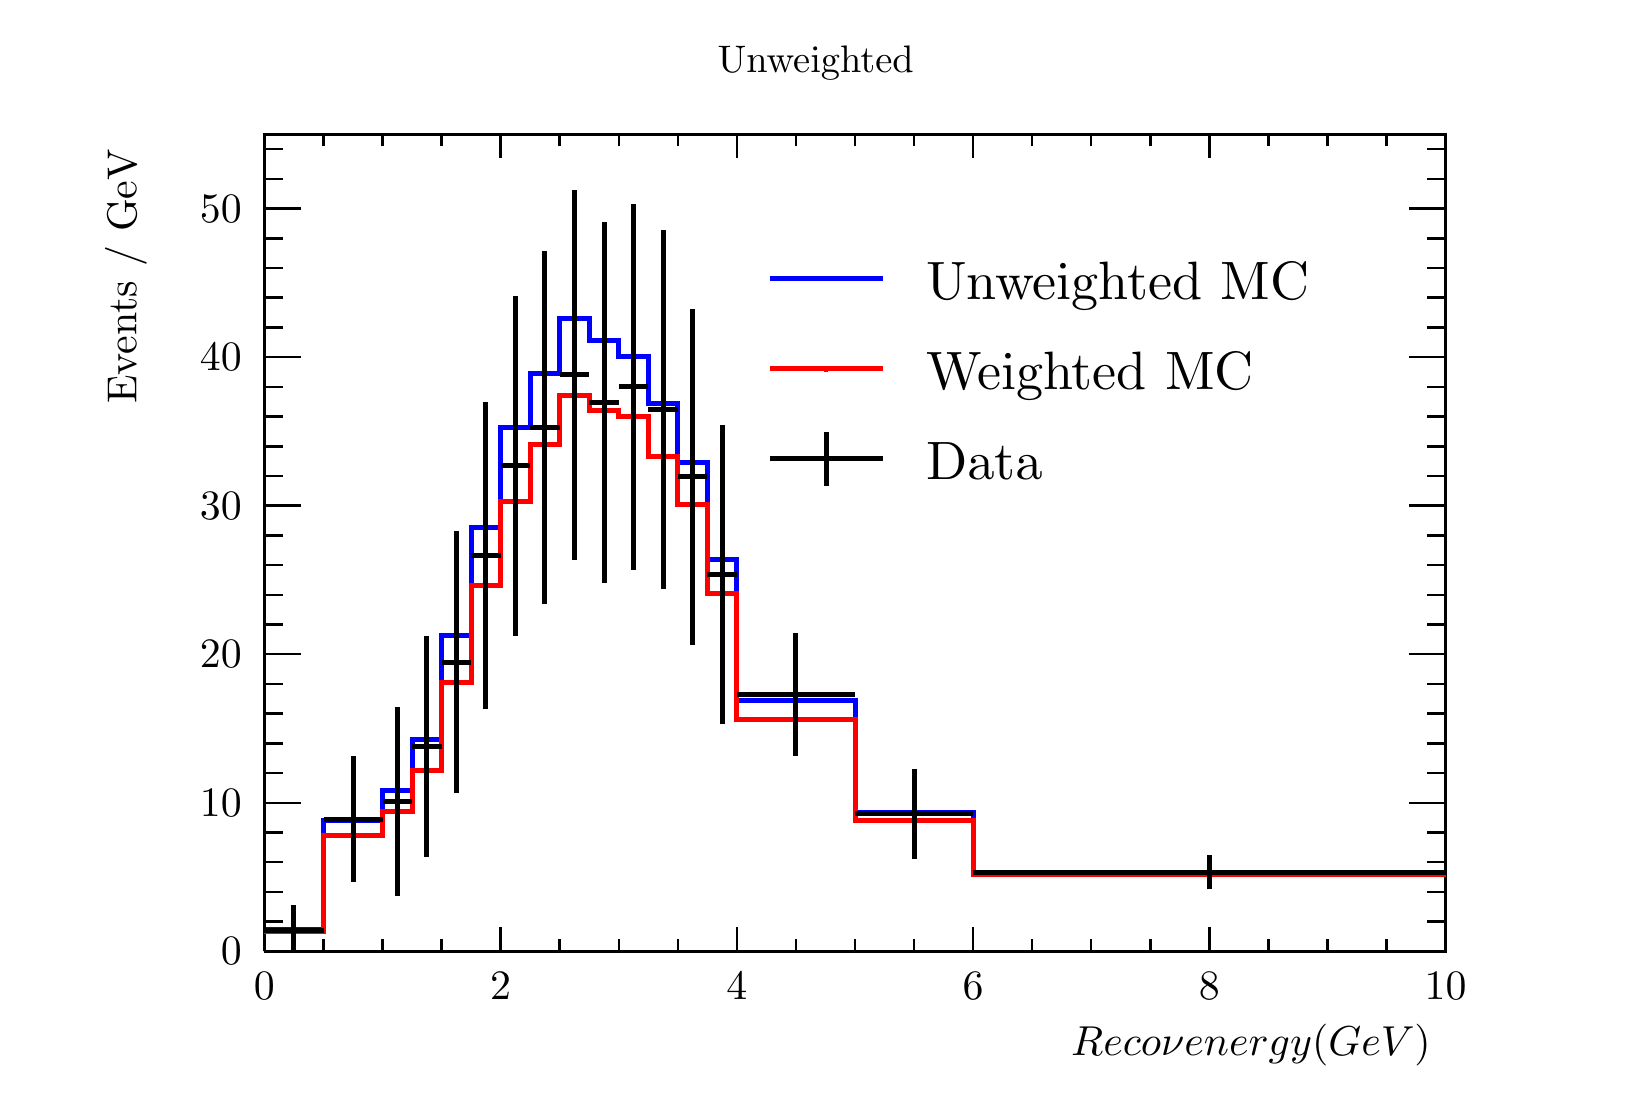
\begin{tikzpicture}
\pgfdeclareplotmark{cross} {
\pgfpathmoveto{\pgfpoint{-0.3\pgfplotmarksize}{\pgfplotmarksize}}
\pgfpathlineto{\pgfpoint{+0.3\pgfplotmarksize}{\pgfplotmarksize}}
\pgfpathlineto{\pgfpoint{+0.3\pgfplotmarksize}{0.3\pgfplotmarksize}}
\pgfpathlineto{\pgfpoint{+1\pgfplotmarksize}{0.3\pgfplotmarksize}}
\pgfpathlineto{\pgfpoint{+1\pgfplotmarksize}{-0.3\pgfplotmarksize}}
\pgfpathlineto{\pgfpoint{+0.3\pgfplotmarksize}{-0.3\pgfplotmarksize}}
\pgfpathlineto{\pgfpoint{+0.3\pgfplotmarksize}{-1.\pgfplotmarksize}}
\pgfpathlineto{\pgfpoint{-0.3\pgfplotmarksize}{-1.\pgfplotmarksize}}
\pgfpathlineto{\pgfpoint{-0.3\pgfplotmarksize}{-0.3\pgfplotmarksize}}
\pgfpathlineto{\pgfpoint{-1.\pgfplotmarksize}{-0.3\pgfplotmarksize}}
\pgfpathlineto{\pgfpoint{-1.\pgfplotmarksize}{0.3\pgfplotmarksize}}
\pgfpathlineto{\pgfpoint{-0.3\pgfplotmarksize}{0.3\pgfplotmarksize}}
\pgfpathclose
\pgfusepathqstroke
}
\pgfdeclareplotmark{cross*} {
\pgfpathmoveto{\pgfpoint{-0.3\pgfplotmarksize}{\pgfplotmarksize}}
\pgfpathlineto{\pgfpoint{+0.3\pgfplotmarksize}{\pgfplotmarksize}}
\pgfpathlineto{\pgfpoint{+0.3\pgfplotmarksize}{0.3\pgfplotmarksize}}
\pgfpathlineto{\pgfpoint{+1\pgfplotmarksize}{0.3\pgfplotmarksize}}
\pgfpathlineto{\pgfpoint{+1\pgfplotmarksize}{-0.3\pgfplotmarksize}}
\pgfpathlineto{\pgfpoint{+0.3\pgfplotmarksize}{-0.3\pgfplotmarksize}}
\pgfpathlineto{\pgfpoint{+0.3\pgfplotmarksize}{-1.\pgfplotmarksize}}
\pgfpathlineto{\pgfpoint{-0.3\pgfplotmarksize}{-1.\pgfplotmarksize}}
\pgfpathlineto{\pgfpoint{-0.3\pgfplotmarksize}{-0.3\pgfplotmarksize}}
\pgfpathlineto{\pgfpoint{-1.\pgfplotmarksize}{-0.3\pgfplotmarksize}}
\pgfpathlineto{\pgfpoint{-1.\pgfplotmarksize}{0.3\pgfplotmarksize}}
\pgfpathlineto{\pgfpoint{-0.3\pgfplotmarksize}{0.3\pgfplotmarksize}}
\pgfpathclose
\pgfusepathqfillstroke
}
\pgfdeclareplotmark{newstar} {
\pgfpathmoveto{\pgfqpoint{0pt}{\pgfplotmarksize}}
\pgfpathlineto{\pgfqpointpolar{44}{0.5\pgfplotmarksize}}
\pgfpathlineto{\pgfqpointpolar{18}{\pgfplotmarksize}}
\pgfpathlineto{\pgfqpointpolar{-20}{0.5\pgfplotmarksize}}
\pgfpathlineto{\pgfqpointpolar{-54}{\pgfplotmarksize}}
\pgfpathlineto{\pgfqpointpolar{-90}{0.5\pgfplotmarksize}}
\pgfpathlineto{\pgfqpointpolar{234}{\pgfplotmarksize}}
\pgfpathlineto{\pgfqpointpolar{198}{0.5\pgfplotmarksize}}
\pgfpathlineto{\pgfqpointpolar{162}{\pgfplotmarksize}}
\pgfpathlineto{\pgfqpointpolar{134}{0.5\pgfplotmarksize}}
\pgfpathclose
\pgfusepathqstroke
}
\pgfdeclareplotmark{newstar*} {
\pgfpathmoveto{\pgfqpoint{0pt}{\pgfplotmarksize}}
\pgfpathlineto{\pgfqpointpolar{44}{0.5\pgfplotmarksize}}
\pgfpathlineto{\pgfqpointpolar{18}{\pgfplotmarksize}}
\pgfpathlineto{\pgfqpointpolar{-20}{0.5\pgfplotmarksize}}
\pgfpathlineto{\pgfqpointpolar{-54}{\pgfplotmarksize}}
\pgfpathlineto{\pgfqpointpolar{-90}{0.5\pgfplotmarksize}}
\pgfpathlineto{\pgfqpointpolar{234}{\pgfplotmarksize}}
\pgfpathlineto{\pgfqpointpolar{198}{0.5\pgfplotmarksize}}
\pgfpathlineto{\pgfqpointpolar{162}{\pgfplotmarksize}}
\pgfpathlineto{\pgfqpointpolar{134}{0.5\pgfplotmarksize}}
\pgfpathclose
\pgfusepathqfillstroke
}
\definecolor{c}{rgb}{1,1,1};
\draw [color=c, fill=c] (0,0) rectangle (20,13.4752);
\draw [color=c, fill=c] (3,1.75177) rectangle (18,12.1277);
\definecolor{c}{rgb}{0,0,0};
\draw [c,line width=0.9] (3,1.75177) -- (3,12.1277) -- (18,12.1277) -- (18,1.75177) -- (3,1.75177);
\definecolor{c}{rgb}{1,1,1};
\draw [color=c, fill=c] (3,1.75177) rectangle (18,12.1277);
\definecolor{c}{rgb}{0,0,0};
\draw [c,line width=0.9] (3,1.75177) -- (3,12.1277) -- (18,12.1277) -- (18,1.75177) -- (3,1.75177);
\definecolor{c}{rgb}{0,0,1};
\draw [c,line width=1.8] (3,2.02999) -- (3.75,2.02999) -- (3.75,3.41537) -- (4.5,3.41537) -- (4.5,3.78866) -- (4.875,3.78866) -- (4.875,4.44674) -- (5.25,4.44674) -- (5.25,5.766) -- (5.625,5.766) -- (5.625,7.13898) -- (6,7.13898) -- (6,8.39894) --
 (6.375,8.39894) -- (6.375,9.08605) -- (6.75,9.08605) -- (6.75,9.7944) -- (7.125,9.7944) -- (7.125,9.50358) -- (7.5,9.50358) -- (7.5,9.31055) -- (7.875,9.31055) -- (7.875,8.7104) -- (8.25,8.7104) -- (8.25,7.96606) -- (8.625,7.96606) --
 (8.625,6.72203) -- (9,6.72203) -- (9,4.93791) -- (10.5,4.93791) -- (10.5,3.51015) -- (12,3.51015) -- (12,2.74254) -- (18,2.74254);
\definecolor{c}{rgb}{0,0,0};
\draw [c,line width=0.9] (3,1.75177) -- (18,1.75177);
\draw [c,line width=0.9] (3,2.05496) -- (3,1.75177);
\draw [c,line width=0.9] (3.75,1.90337) -- (3.75,1.75177);
\draw [c,line width=0.9] (4.5,1.90337) -- (4.5,1.75177);
\draw [c,line width=0.9] (5.25,1.90337) -- (5.25,1.75177);
\draw [c,line width=0.9] (6,2.05496) -- (6,1.75177);
\draw [c,line width=0.9] (6.75,1.90337) -- (6.75,1.75177);
\draw [c,line width=0.9] (7.5,1.90337) -- (7.5,1.75177);
\draw [c,line width=0.9] (8.25,1.90337) -- (8.25,1.75177);
\draw [c,line width=0.9] (9,2.05496) -- (9,1.75177);
\draw [c,line width=0.9] (9.75,1.90337) -- (9.75,1.75177);
\draw [c,line width=0.9] (10.5,1.90337) -- (10.5,1.75177);
\draw [c,line width=0.9] (11.25,1.90337) -- (11.25,1.75177);
\draw [c,line width=0.9] (12,2.05496) -- (12,1.75177);
\draw [c,line width=0.9] (12.75,1.90337) -- (12.75,1.75177);
\draw [c,line width=0.9] (13.5,1.90337) -- (13.5,1.75177);
\draw [c,line width=0.9] (14.25,1.90337) -- (14.25,1.75177);
\draw [c,line width=0.9] (15,2.05496) -- (15,1.75177);
\draw [c,line width=0.9] (15.75,1.90337) -- (15.75,1.75177);
\draw [c,line width=0.9] (16.5,1.90337) -- (16.5,1.75177);
\draw [c,line width=0.9] (17.25,1.90337) -- (17.25,1.75177);
\draw [c,line width=0.9] (18,2.05496) -- (18,1.75177);
\draw [anchor=base] (3,1.14539) node[scale=1.51215, color=c, rotate=0]{0};
\draw [anchor=base] (6,1.14539) node[scale=1.51215, color=c, rotate=0]{2};
\draw [anchor=base] (9,1.14539) node[scale=1.51215, color=c, rotate=0]{4};
\draw [anchor=base] (12,1.14539) node[scale=1.51215, color=c, rotate=0]{6};
\draw [anchor=base] (15,1.14539) node[scale=1.51215, color=c, rotate=0]{8};
\draw [anchor=base] (18,1.14539) node[scale=1.51215, color=c, rotate=0]{10};
\draw [anchor= east] (18,0.565957) node[scale=1.51215, color=c, rotate=0]{$Reco \nu energy (GeV)$};
\draw [c,line width=0.9] (3,12.1277) -- (18,12.1277);
\draw [c,line width=0.9] (3,11.8245) -- (3,12.1277);
\draw [c,line width=0.9] (3.75,11.9761) -- (3.75,12.1277);
\draw [c,line width=0.9] (4.5,11.9761) -- (4.5,12.1277);
\draw [c,line width=0.9] (5.25,11.9761) -- (5.25,12.1277);
\draw [c,line width=0.9] (6,11.8245) -- (6,12.1277);
\draw [c,line width=0.9] (6.75,11.9761) -- (6.75,12.1277);
\draw [c,line width=0.9] (7.5,11.9761) -- (7.5,12.1277);
\draw [c,line width=0.9] (8.25,11.9761) -- (8.25,12.1277);
\draw [c,line width=0.9] (9,11.8245) -- (9,12.1277);
\draw [c,line width=0.9] (9.75,11.9761) -- (9.75,12.1277);
\draw [c,line width=0.9] (10.5,11.9761) -- (10.5,12.1277);
\draw [c,line width=0.9] (11.25,11.9761) -- (11.25,12.1277);
\draw [c,line width=0.9] (12,11.8245) -- (12,12.1277);
\draw [c,line width=0.9] (12.75,11.9761) -- (12.75,12.1277);
\draw [c,line width=0.9] (13.5,11.9761) -- (13.5,12.1277);
\draw [c,line width=0.9] (14.25,11.9761) -- (14.25,12.1277);
\draw [c,line width=0.9] (15,11.8245) -- (15,12.1277);
\draw [c,line width=0.9] (15.75,11.9761) -- (15.75,12.1277);
\draw [c,line width=0.9] (16.5,11.9761) -- (16.5,12.1277);
\draw [c,line width=0.9] (17.25,11.9761) -- (17.25,12.1277);
\draw [c,line width=0.9] (18,11.8245) -- (18,12.1277);
\draw [c,line width=0.9] (3,1.75177) -- (3,12.1277);
\draw [c,line width=0.9] (3.462,1.75177) -- (3,1.75177);
\draw [c,line width=0.9] (3.231,2.12908) -- (3,2.12908);
\draw [c,line width=0.9] (3.231,2.50638) -- (3,2.50638);
\draw [c,line width=0.9] (3.231,2.88369) -- (3,2.88369);
\draw [c,line width=0.9] (3.231,3.26099) -- (3,3.26099);
\draw [c,line width=0.9] (3.462,3.6383) -- (3,3.6383);
\draw [c,line width=0.9] (3.231,4.0156) -- (3,4.0156);
\draw [c,line width=0.9] (3.231,4.39291) -- (3,4.39291);
\draw [c,line width=0.9] (3.231,4.77021) -- (3,4.77021);
\draw [c,line width=0.9] (3.231,5.14752) -- (3,5.14752);
\draw [c,line width=0.9] (3.462,5.52482) -- (3,5.52482);
\draw [c,line width=0.9] (3.231,5.90213) -- (3,5.90213);
\draw [c,line width=0.9] (3.231,6.27943) -- (3,6.27943);
\draw [c,line width=0.9] (3.231,6.65674) -- (3,6.65674);
\draw [c,line width=0.9] (3.231,7.03404) -- (3,7.03404);
\draw [c,line width=0.9] (3.462,7.41135) -- (3,7.41135);
\draw [c,line width=0.9] (3.231,7.78865) -- (3,7.78865);
\draw [c,line width=0.9] (3.231,8.16596) -- (3,8.16596);
\draw [c,line width=0.9] (3.231,8.54326) -- (3,8.54326);
\draw [c,line width=0.9] (3.231,8.92057) -- (3,8.92057);
\draw [c,line width=0.9] (3.462,9.29787) -- (3,9.29787);
\draw [c,line width=0.9] (3.231,9.67518) -- (3,9.67518);
\draw [c,line width=0.9] (3.231,10.0525) -- (3,10.0525);
\draw [c,line width=0.9] (3.231,10.4298) -- (3,10.4298);
\draw [c,line width=0.9] (3.231,10.8071) -- (3,10.8071);
\draw [c,line width=0.9] (3.462,11.1844) -- (3,11.1844);
\draw [c,line width=0.9] (3.462,11.1844) -- (3,11.1844);
\draw [c,line width=0.9] (3.231,11.5617) -- (3,11.5617);
\draw [c,line width=0.9] (3.231,11.939) -- (3,11.939);
\draw [anchor= east] (2.9,1.75177) node[scale=1.51215, color=c, rotate=0]{0};
\draw [anchor= east] (2.9,3.6383) node[scale=1.51215, color=c, rotate=0]{10};
\draw [anchor= east] (2.9,5.52482) node[scale=1.51215, color=c, rotate=0]{20};
\draw [anchor= east] (2.9,7.41135) node[scale=1.51215, color=c, rotate=0]{30};
\draw [anchor= east] (2.9,9.29787) node[scale=1.51215, color=c, rotate=0]{40};
\draw [anchor= east] (2.9,11.1844) node[scale=1.51215, color=c, rotate=0]{50};
\draw [anchor= east] (1.24,12.1277) node[scale=1.51215, color=c, rotate=90]{Events / GeV};
\draw [c,line width=0.9] (18,1.75177) -- (18,12.1277);
\draw [c,line width=0.9] (17.538,1.75177) -- (18,1.75177);
\draw [c,line width=0.9] (17.769,2.12908) -- (18,2.12908);
\draw [c,line width=0.9] (17.769,2.50638) -- (18,2.50638);
\draw [c,line width=0.9] (17.769,2.88369) -- (18,2.88369);
\draw [c,line width=0.9] (17.769,3.26099) -- (18,3.26099);
\draw [c,line width=0.9] (17.538,3.6383) -- (18,3.6383);
\draw [c,line width=0.9] (17.769,4.0156) -- (18,4.0156);
\draw [c,line width=0.9] (17.769,4.39291) -- (18,4.39291);
\draw [c,line width=0.9] (17.769,4.77021) -- (18,4.77021);
\draw [c,line width=0.9] (17.769,5.14752) -- (18,5.14752);
\draw [c,line width=0.9] (17.538,5.52482) -- (18,5.52482);
\draw [c,line width=0.9] (17.769,5.90213) -- (18,5.90213);
\draw [c,line width=0.9] (17.769,6.27943) -- (18,6.27943);
\draw [c,line width=0.9] (17.769,6.65674) -- (18,6.65674);
\draw [c,line width=0.9] (17.769,7.03404) -- (18,7.03404);
\draw [c,line width=0.9] (17.538,7.41135) -- (18,7.41135);
\draw [c,line width=0.9] (17.769,7.78865) -- (18,7.78865);
\draw [c,line width=0.9] (17.769,8.16596) -- (18,8.16596);
\draw [c,line width=0.9] (17.769,8.54326) -- (18,8.54326);
\draw [c,line width=0.9] (17.769,8.92057) -- (18,8.92057);
\draw [c,line width=0.9] (17.538,9.29787) -- (18,9.29787);
\draw [c,line width=0.9] (17.769,9.67518) -- (18,9.67518);
\draw [c,line width=0.9] (17.769,10.0525) -- (18,10.0525);
\draw [c,line width=0.9] (17.769,10.4298) -- (18,10.4298);
\draw [c,line width=0.9] (17.769,10.8071) -- (18,10.8071);
\draw [c,line width=0.9] (17.538,11.1844) -- (18,11.1844);
\draw [c,line width=0.9] (17.538,11.1844) -- (18,11.1844);
\draw [c,line width=0.9] (17.769,11.5617) -- (18,11.5617);
\draw [c,line width=0.9] (17.769,11.939) -- (18,11.939);
\definecolor{c}{rgb}{1,1,1};
\draw [color=c, fill=c] (2,12.6667) rectangle (18,13.4078);
\definecolor{c}{rgb}{0,0,0};
\draw (10,13.0372) node[scale=1.38614, color=c, rotate=0]{Unweighted};
\definecolor{c}{rgb}{1,0,0};
\draw [c,line width=1.8] (3,2.00665) -- (3.75,2.00665) -- (3.75,3.2233) -- (4.5,3.2233) -- (4.5,3.52806) -- (4.875,3.52806) -- (4.875,4.05181) -- (5.25,4.05181) -- (5.25,5.16925) -- (5.625,5.16925) -- (5.625,6.39298) -- (6,6.39298) -- (6,7.46518) --
 (6.375,7.46518) -- (6.375,8.18436) -- (6.75,8.18436) -- (6.75,8.81487) -- (7.125,8.81487) -- (7.125,8.61643) -- (7.5,8.61643) -- (7.5,8.54439) -- (7.875,8.54439) -- (7.875,8.03468) -- (8.25,8.03468) -- (8.25,7.42528) -- (8.625,7.42528) --
 (8.625,6.2965) -- (9,6.2965) -- (9,4.69037) -- (10.5,4.69037) -- (10.5,3.4118) -- (12,3.4118) -- (12,2.72153) -- (18,2.72153);
\definecolor{c}{rgb}{0,0,0};
\draw [c,line width=1.8] (3.375,1.75177) -- (3.375,2.0196);
\draw [c,line width=1.8] (3.375,2.0196) -- (3.375,2.33748);
\draw [c,line width=1.8] (3,2.0196) -- (3.375,2.0196);
\draw [c,line width=1.8] (3.375,2.0196) -- (3.75,2.0196);
\foreach \P in {(3.375,2.0196)}{\draw[mark options={color=c,fill=c},mark size=2.402402pt, line width=0.000000pt, mark=*,mark size=1pt] plot coordinates {\P};}
\draw [c,line width=1.8] (4.125,2.63575) -- (4.125,3.43196);
\draw [c,line width=1.8] (4.125,3.43196) -- (4.125,4.22817);
\draw [c,line width=1.8] (3.75,3.43196) -- (4.125,3.43196);
\draw [c,line width=1.8] (4.125,3.43196) -- (4.5,3.43196);
\foreach \P in {(4.125,3.43196)}{\draw[mark options={color=c,fill=c},mark size=2.402402pt, line width=0.000000pt, mark=*,mark size=1pt] plot coordinates {\P};}
\draw [c,line width=1.8] (4.6875,2.45991) -- (4.6875,3.65985);
\draw [c,line width=1.8] (4.6875,3.65985) -- (4.6875,4.85978);
\draw [c,line width=1.8] (4.5,3.65985) -- (4.6875,3.65985);
\draw [c,line width=1.8] (4.6875,3.65985) -- (4.875,3.65985);
\foreach \P in {(4.6875,3.65985)}{\draw[mark options={color=c,fill=c},mark size=2.402402pt, line width=0.000000pt, mark=*,mark size=1pt] plot coordinates {\P};}
\draw [c,line width=1.8] (5.0625,2.95418) -- (5.0625,4.35604);
\draw [c,line width=1.8] (5.0625,4.35604) -- (5.0625,5.7579);
\draw [c,line width=1.8] (4.875,4.35604) -- (5.0625,4.35604);
\draw [c,line width=1.8] (5.0625,4.35604) -- (5.25,4.35604);
\foreach \P in {(5.0625,4.35604)}{\draw[mark options={color=c,fill=c},mark size=2.402402pt, line width=0.000000pt, mark=*,mark size=1pt] plot coordinates {\P};}
\draw [c,line width=1.8] (5.4375,3.75845) -- (5.4375,5.42285);
\draw [c,line width=1.8] (5.4375,5.42285) -- (5.4375,7.08725);
\draw [c,line width=1.8] (5.25,5.42285) -- (5.4375,5.42285);
\draw [c,line width=1.8] (5.4375,5.42285) -- (5.625,5.42285);
\foreach \P in {(5.4375,5.42285)}{\draw[mark options={color=c,fill=c},mark size=2.402402pt, line width=0.000000pt, mark=*,mark size=1pt] plot coordinates {\P};}
\draw [c,line width=1.8] (5.8125,4.82855) -- (5.8125,6.77561);
\draw [c,line width=1.8] (5.8125,6.77561) -- (5.8125,8.72267);
\draw [c,line width=1.8] (5.625,6.77561) -- (5.8125,6.77561);
\draw [c,line width=1.8] (5.8125,6.77561) -- (6,6.77561);
\foreach \P in {(5.8125,6.77561)}{\draw[mark options={color=c,fill=c},mark size=2.402402pt, line width=0.000000pt, mark=*,mark size=1pt] plot coordinates {\P};}
\draw [c,line width=1.8] (6.1875,5.76145) -- (6.1875,7.91867);
\draw [c,line width=1.8] (6.1875,7.91867) -- (6.1875,10.0759);
\draw [c,line width=1.8] (6,7.91867) -- (6.1875,7.91867);
\draw [c,line width=1.8] (6.1875,7.91867) -- (6.375,7.91867);
\foreach \P in {(6.1875,7.91867)}{\draw[mark options={color=c,fill=c},mark size=2.402402pt, line width=0.000000pt, mark=*,mark size=1pt] plot coordinates {\P};}
\draw [c,line width=1.8] (6.5625,6.16706) -- (6.5625,8.40828);
\draw [c,line width=1.8] (6.5625,8.40828) -- (6.5625,10.6495);
\draw [c,line width=1.8] (6.375,8.40828) -- (6.5625,8.40828);
\draw [c,line width=1.8] (6.5625,8.40828) -- (6.75,8.40828);
\foreach \P in {(6.5625,8.40828)}{\draw[mark options={color=c,fill=c},mark size=2.402402pt, line width=0.000000pt, mark=*,mark size=1pt] plot coordinates {\P};}
\draw [c,line width=1.8] (6.9375,6.72122) -- (6.9375,9.07142);
\draw [c,line width=1.8] (6.9375,9.07142) -- (6.9375,11.4216);
\draw [c,line width=1.8] (6.75,9.07142) -- (6.9375,9.07142);
\draw [c,line width=1.8] (6.9375,9.07142) -- (7.125,9.07142);
\foreach \P in {(6.9375,9.07142)}{\draw[mark options={color=c,fill=c},mark size=2.402402pt, line width=0.000000pt, mark=*,mark size=1pt] plot coordinates {\P};}
\draw [c,line width=1.8] (7.3125,6.42759) -- (7.3125,8.72083);
\draw [c,line width=1.8] (7.3125,8.72083) -- (7.3125,11.0141);
\draw [c,line width=1.8] (7.125,8.72083) -- (7.3125,8.72083);
\draw [c,line width=1.8] (7.3125,8.72083) -- (7.5,8.72083);
\foreach \P in {(7.3125,8.72083)}{\draw[mark options={color=c,fill=c},mark size=2.402402pt, line width=0.000000pt, mark=*,mark size=1pt] plot coordinates {\P};}
\draw [c,line width=1.8] (7.6875,6.5962) -- (7.6875,8.92236);
\draw [c,line width=1.8] (7.6875,8.92236) -- (7.6875,11.2485);
\draw [c,line width=1.8] (7.5,8.92236) -- (7.6875,8.92236);
\draw [c,line width=1.8] (7.6875,8.92236) -- (7.875,8.92236);
\foreach \P in {(7.6875,8.92236)}{\draw[mark options={color=c,fill=c},mark size=2.402402pt, line width=0.000000pt, mark=*,mark size=1pt] plot coordinates {\P};}
\draw [c,line width=1.8] (8.0625,6.35619) -- (8.0625,8.63531);
\draw [c,line width=1.8] (8.0625,8.63531) -- (8.0625,10.9144);
\draw [c,line width=1.8] (7.875,8.63531) -- (8.0625,8.63531);
\draw [c,line width=1.8] (8.0625,8.63531) -- (8.25,8.63531);
\foreach \P in {(8.0625,8.63531)}{\draw[mark options={color=c,fill=c},mark size=2.402402pt, line width=0.000000pt, mark=*,mark size=1pt] plot coordinates {\P};}
\draw [c,line width=1.8] (8.4375,5.64734) -- (8.4375,7.78021);
\draw [c,line width=1.8] (8.4375,7.78021) -- (8.4375,9.91307);
\draw [c,line width=1.8] (8.25,7.78021) -- (8.4375,7.78021);
\draw [c,line width=1.8] (8.4375,7.78021) -- (8.625,7.78021);
\foreach \P in {(8.4375,7.78021)}{\draw[mark options={color=c,fill=c},mark size=2.402402pt, line width=0.000000pt, mark=*,mark size=1pt] plot coordinates {\P};}
\draw [c,line width=1.8] (8.8125,4.63398) -- (8.8125,6.53355);
\draw [c,line width=1.8] (8.8125,6.53355) -- (8.8125,8.43312);
\draw [c,line width=1.8] (8.625,6.53355) -- (8.8125,6.53355);
\draw [c,line width=1.8] (8.8125,6.53355) -- (9,6.53355);
\foreach \P in {(8.8125,6.53355)}{\draw[mark options={color=c,fill=c},mark size=2.402402pt, line width=0.000000pt, mark=*,mark size=1pt] plot coordinates {\P};}
\draw [c,line width=1.8] (9.75,4.22812) -- (9.75,5.01243);
\draw [c,line width=1.8] (9.75,5.01243) -- (9.75,5.79673);
\draw [c,line width=1.8] (9,5.01243) -- (9.75,5.01243);
\draw [c,line width=1.8] (9.75,5.01243) -- (10.5,5.01243);
\foreach \P in {(9.75,5.01243)}{\draw[mark options={color=c,fill=c},mark size=2.402402pt, line width=0.000000pt, mark=*,mark size=1pt] plot coordinates {\P};}
\draw [c,line width=1.8] (11.25,2.92308) -- (11.25,3.49685);
\draw [c,line width=1.8] (11.25,3.49685) -- (11.25,4.07062);
\draw [c,line width=1.8] (10.5,3.49685) -- (11.25,3.49685);
\draw [c,line width=1.8] (11.25,3.49685) -- (12,3.49685);
\foreach \P in {(11.25,3.49685)}{\draw[mark options={color=c,fill=c},mark size=2.402402pt, line width=0.000000pt, mark=*,mark size=1pt] plot coordinates {\P};}
\draw [c,line width=1.8] (15,2.53815) -- (15,2.75575);
\draw [c,line width=1.8] (15,2.75575) -- (15,2.97335);
\draw [c,line width=1.8] (12,2.75575) -- (15,2.75575);
\draw [c,line width=1.8] (15,2.75575) -- (18,2.75575);
\foreach \P in {(15,2.75575)}{\draw[mark options={color=c,fill=c},mark size=2.402402pt, line width=0.000000pt, mark=*,mark size=1pt] plot coordinates {\P};}
\definecolor{c}{rgb}{1,1,1};
\draw [color=c, fill=c] (9.10638,7.43262) rectangle (17.3333,10.8652);
\definecolor{c}{rgb}{0,0,0};
\draw [anchor=base west] (11.1631,10.0357) node[scale=1.95319, color=c, rotate=0]{Unweighted MC};
\definecolor{c}{rgb}{0,0,1};
\draw [c,line width=1.8] (9.41489,10.2931) -- (10.8546,10.2931);
\definecolor{c}{rgb}{0,0,0};
\draw [anchor=base west] (11.1631,8.89149) node[scale=1.95319, color=c, rotate=0]{Weighted MC};
\definecolor{c}{rgb}{1,1,1};
\draw [c, fill=c] (9.41489,8.74846) -- (10.8546,8.74846) -- (10.8546,9.54941) -- (9.41489,9.54941);
\definecolor{c}{rgb}{1,0,0};
\draw [c,line width=1.8] (9.41489,9.14894) -- (10.8546,9.14894);
\foreach \P in {(10.1348,9.14894)}{\draw[mark options={color=c,fill=c},mark size=2.402402pt, line width=0.000000pt, mark=*,mark size=1pt] plot coordinates {\P};}
\definecolor{c}{rgb}{0,0,0};
\draw [anchor=base west] (11.1631,7.74728) node[scale=1.95319, color=c, rotate=0]{Data};
\draw [c,line width=1.8] (9.41489,8.00473) -- (10.8546,8.00473);
\draw [c,line width=1.8] (10.1348,7.66147) -- (10.1348,8.34799);
\end{tikzpicture}

		\end{adjustbox}
		\caption{RHC \anue}
	\end{subfigure}
	\caption[Comparison of weighted and unweighted far detector MC with mock data]{Comparison of weighted and unweighted far detector MC with mock data. Here, $\dcp=\pi$.}
	\label{fig:reweightedSamples}
\end{figure}

Additionally, the ratio to data for each of the MC samples is shown in \citefig{fig:reweightedSamplesRatio}.
\citefig{fig:reweightedSamplesRatio} also shows the calculated $\chi^{2}$ values for each MC sample when compared with the `mock data'.
Here, one can see that at this particular set of oscillation parameters the $\chi^{2}$ for all samples apart from \nue RHC is lower for the weighted sample than the unweighted one.
This indicates that the reweighting is bringing the MC closer to the mock data.

\begin{figure}[h]
	\begin{subfigure}[t]{.5\linewidth}
		\begin{adjustbox}{max totalsize=\linewidth, center}
			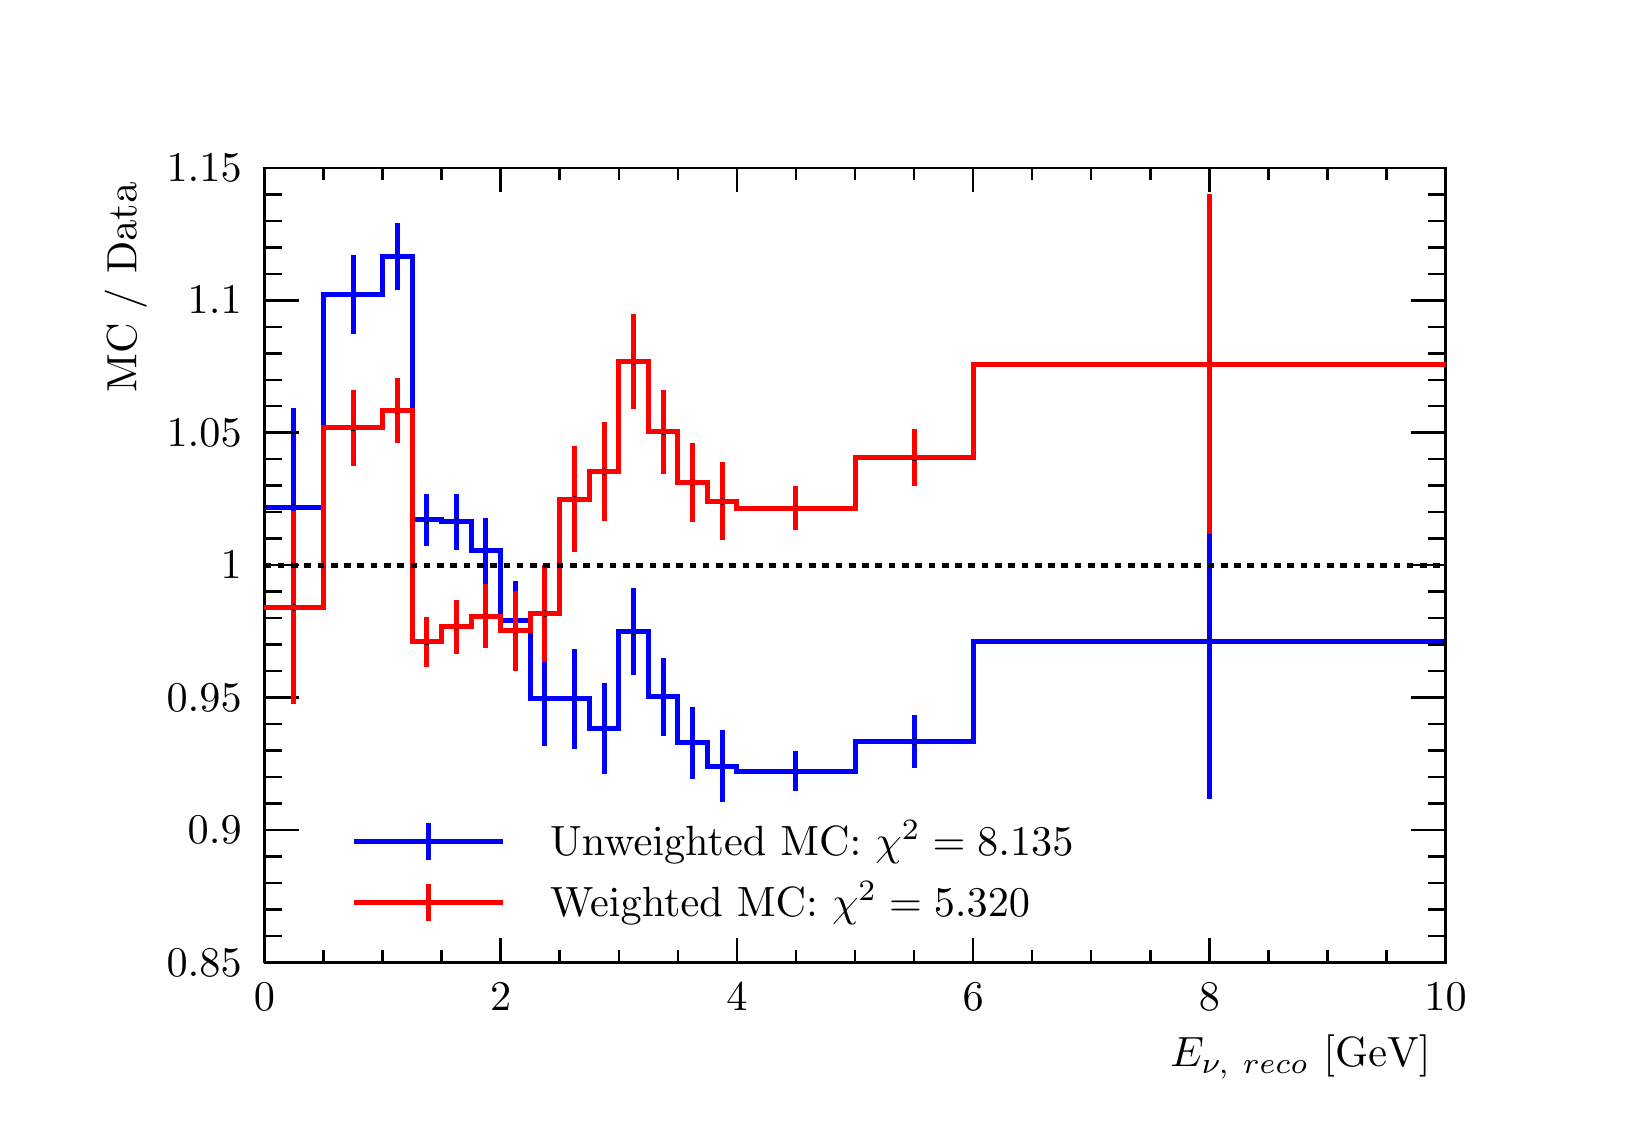
\begin{tikzpicture}
\pgfdeclareplotmark{cross} {
\pgfpathmoveto{\pgfpoint{-0.3\pgfplotmarksize}{\pgfplotmarksize}}
\pgfpathlineto{\pgfpoint{+0.3\pgfplotmarksize}{\pgfplotmarksize}}
\pgfpathlineto{\pgfpoint{+0.3\pgfplotmarksize}{0.3\pgfplotmarksize}}
\pgfpathlineto{\pgfpoint{+1\pgfplotmarksize}{0.3\pgfplotmarksize}}
\pgfpathlineto{\pgfpoint{+1\pgfplotmarksize}{-0.3\pgfplotmarksize}}
\pgfpathlineto{\pgfpoint{+0.3\pgfplotmarksize}{-0.3\pgfplotmarksize}}
\pgfpathlineto{\pgfpoint{+0.3\pgfplotmarksize}{-1.\pgfplotmarksize}}
\pgfpathlineto{\pgfpoint{-0.3\pgfplotmarksize}{-1.\pgfplotmarksize}}
\pgfpathlineto{\pgfpoint{-0.3\pgfplotmarksize}{-0.3\pgfplotmarksize}}
\pgfpathlineto{\pgfpoint{-1.\pgfplotmarksize}{-0.3\pgfplotmarksize}}
\pgfpathlineto{\pgfpoint{-1.\pgfplotmarksize}{0.3\pgfplotmarksize}}
\pgfpathlineto{\pgfpoint{-0.3\pgfplotmarksize}{0.3\pgfplotmarksize}}
\pgfpathclose
\pgfusepathqstroke
}
\pgfdeclareplotmark{cross*} {
\pgfpathmoveto{\pgfpoint{-0.3\pgfplotmarksize}{\pgfplotmarksize}}
\pgfpathlineto{\pgfpoint{+0.3\pgfplotmarksize}{\pgfplotmarksize}}
\pgfpathlineto{\pgfpoint{+0.3\pgfplotmarksize}{0.3\pgfplotmarksize}}
\pgfpathlineto{\pgfpoint{+1\pgfplotmarksize}{0.3\pgfplotmarksize}}
\pgfpathlineto{\pgfpoint{+1\pgfplotmarksize}{-0.3\pgfplotmarksize}}
\pgfpathlineto{\pgfpoint{+0.3\pgfplotmarksize}{-0.3\pgfplotmarksize}}
\pgfpathlineto{\pgfpoint{+0.3\pgfplotmarksize}{-1.\pgfplotmarksize}}
\pgfpathlineto{\pgfpoint{-0.3\pgfplotmarksize}{-1.\pgfplotmarksize}}
\pgfpathlineto{\pgfpoint{-0.3\pgfplotmarksize}{-0.3\pgfplotmarksize}}
\pgfpathlineto{\pgfpoint{-1.\pgfplotmarksize}{-0.3\pgfplotmarksize}}
\pgfpathlineto{\pgfpoint{-1.\pgfplotmarksize}{0.3\pgfplotmarksize}}
\pgfpathlineto{\pgfpoint{-0.3\pgfplotmarksize}{0.3\pgfplotmarksize}}
\pgfpathclose
\pgfusepathqfillstroke
}
\pgfdeclareplotmark{newstar} {
\pgfpathmoveto{\pgfqpoint{0pt}{\pgfplotmarksize}}
\pgfpathlineto{\pgfqpointpolar{44}{0.5\pgfplotmarksize}}
\pgfpathlineto{\pgfqpointpolar{18}{\pgfplotmarksize}}
\pgfpathlineto{\pgfqpointpolar{-20}{0.5\pgfplotmarksize}}
\pgfpathlineto{\pgfqpointpolar{-54}{\pgfplotmarksize}}
\pgfpathlineto{\pgfqpointpolar{-90}{0.5\pgfplotmarksize}}
\pgfpathlineto{\pgfqpointpolar{234}{\pgfplotmarksize}}
\pgfpathlineto{\pgfqpointpolar{198}{0.5\pgfplotmarksize}}
\pgfpathlineto{\pgfqpointpolar{162}{\pgfplotmarksize}}
\pgfpathlineto{\pgfqpointpolar{134}{0.5\pgfplotmarksize}}
\pgfpathclose
\pgfusepathqstroke
}
\pgfdeclareplotmark{newstar*} {
\pgfpathmoveto{\pgfqpoint{0pt}{\pgfplotmarksize}}
\pgfpathlineto{\pgfqpointpolar{44}{0.5\pgfplotmarksize}}
\pgfpathlineto{\pgfqpointpolar{18}{\pgfplotmarksize}}
\pgfpathlineto{\pgfqpointpolar{-20}{0.5\pgfplotmarksize}}
\pgfpathlineto{\pgfqpointpolar{-54}{\pgfplotmarksize}}
\pgfpathlineto{\pgfqpointpolar{-90}{0.5\pgfplotmarksize}}
\pgfpathlineto{\pgfqpointpolar{234}{\pgfplotmarksize}}
\pgfpathlineto{\pgfqpointpolar{198}{0.5\pgfplotmarksize}}
\pgfpathlineto{\pgfqpointpolar{162}{\pgfplotmarksize}}
\pgfpathlineto{\pgfqpointpolar{134}{0.5\pgfplotmarksize}}
\pgfpathclose
\pgfusepathqfillstroke
}
\definecolor{c}{rgb}{1,1,1};
\draw [color=c, fill=c] (0,0) rectangle (20,13.639);
\draw [color=c, fill=c] (3,1.77307) rectangle (18,11.8659);
\definecolor{c}{rgb}{0,0,0};
\draw [c,line width=0.9] (3,1.77307) -- (3,11.8659) -- (18,11.8659) -- (18,1.77307) -- (3,1.77307);
\definecolor{c}{rgb}{1,1,1};
\draw [color=c, fill=c] (3,1.77307) rectangle (18,11.8659);
\definecolor{c}{rgb}{0,0,0};
\draw [c,line width=0.9] (3,1.77307) -- (3,11.8659) -- (18,11.8659) -- (18,1.77307) -- (3,1.77307);
\definecolor{c}{rgb}{0,0,1};
\draw [c,line width=1.8] (3.375,6.29488) -- (3.375,7.55685);
\draw [c,line width=1.8] (3.375,7.55685) -- (3.375,8.81881);
\definecolor{c}{rgb}{0,0,0};
\foreach \P in {(3.375,7.55685)}{\draw[mark options={color=c,fill=c},mark size=2.402402pt, line width=0.000000pt, mark=*,mark size=1pt] plot coordinates {\P};}
\definecolor{c}{rgb}{0,0,1};
\draw [c,line width=1.8] (4.125,9.75489) -- (4.125,10.2541);
\draw [c,line width=1.8] (4.125,10.2541) -- (4.125,10.7532);
\definecolor{c}{rgb}{0,0,0};
\foreach \P in {(4.125,10.2541)}{\draw[mark options={color=c,fill=c},mark size=2.402402pt, line width=0.000000pt, mark=*,mark size=1pt] plot coordinates {\P};}
\definecolor{c}{rgb}{0,0,1};
\draw [c,line width=1.8] (4.6875,10.3081) -- (4.6875,10.7391);
\draw [c,line width=1.8] (4.6875,10.7391) -- (4.6875,11.1702);
\definecolor{c}{rgb}{0,0,0};
\foreach \P in {(4.6875,10.7391)}{\draw[mark options={color=c,fill=c},mark size=2.402402pt, line width=0.000000pt, mark=*,mark size=1pt] plot coordinates {\P};}
\definecolor{c}{rgb}{0,0,1};
\draw [c,line width=1.8] (5.0625,7.06515) -- (5.0625,7.39448);
\draw [c,line width=1.8] (5.0625,7.39448) -- (5.0625,7.72382);
\definecolor{c}{rgb}{0,0,0};
\foreach \P in {(5.0625,7.39448)}{\draw[mark options={color=c,fill=c},mark size=2.402402pt, line width=0.000000pt, mark=*,mark size=1pt] plot coordinates {\P};}
\definecolor{c}{rgb}{0,0,1};
\draw [c,line width=1.8] (5.4375,7.01789) -- (5.4375,7.37106);
\draw [c,line width=1.8] (5.4375,7.37106) -- (5.4375,7.72423);
\definecolor{c}{rgb}{0,0,0};
\foreach \P in {(5.4375,7.37106)}{\draw[mark options={color=c,fill=c},mark size=2.402402pt, line width=0.000000pt, mark=*,mark size=1pt] plot coordinates {\P};}
\definecolor{c}{rgb}{0,0,1};
\draw [c,line width=1.8] (5.8125,6.58502) -- (5.8125,7.00202);
\draw [c,line width=1.8] (5.8125,7.00202) -- (5.8125,7.41901);
\definecolor{c}{rgb}{0,0,0};
\foreach \P in {(5.8125,7.00202)}{\draw[mark options={color=c,fill=c},mark size=2.402402pt, line width=0.000000pt, mark=*,mark size=1pt] plot coordinates {\P};}
\definecolor{c}{rgb}{0,0,1};
\draw [c,line width=1.8] (6.1875,5.60236) -- (6.1875,6.11319);
\draw [c,line width=1.8] (6.1875,6.11319) -- (6.1875,6.62403);
\definecolor{c}{rgb}{0,0,0};
\foreach \P in {(6.1875,6.11319)}{\draw[mark options={color=c,fill=c},mark size=2.402402pt, line width=0.000000pt, mark=*,mark size=1pt] plot coordinates {\P};}
\definecolor{c}{rgb}{0,0,1};
\draw [c,line width=1.8] (6.5625,4.52926) -- (6.5625,5.12907);
\draw [c,line width=1.8] (6.5625,5.12907) -- (6.5625,5.72889);
\definecolor{c}{rgb}{0,0,0};
\foreach \P in {(6.5625,5.12907)}{\draw[mark options={color=c,fill=c},mark size=2.402402pt, line width=0.000000pt, mark=*,mark size=1pt] plot coordinates {\P};}
\definecolor{c}{rgb}{0,0,1};
\draw [c,line width=1.8] (6.9375,4.48615) -- (6.9375,5.12235);
\draw [c,line width=1.8] (6.9375,5.12235) -- (6.9375,5.75854);
\definecolor{c}{rgb}{0,0,0};
\foreach \P in {(6.9375,5.12235)}{\draw[mark options={color=c,fill=c},mark size=2.402402pt, line width=0.000000pt, mark=*,mark size=1pt] plot coordinates {\P};}
\definecolor{c}{rgb}{0,0,1};
\draw [c,line width=1.8] (7.3125,4.16193) -- (7.3125,4.74369);
\draw [c,line width=1.8] (7.3125,4.74369) -- (7.3125,5.32546);
\definecolor{c}{rgb}{0,0,0};
\foreach \P in {(7.3125,4.74369)}{\draw[mark options={color=c,fill=c},mark size=2.402402pt, line width=0.000000pt, mark=*,mark size=1pt] plot coordinates {\P};}
\definecolor{c}{rgb}{0,0,1};
\draw [c,line width=1.8] (7.6875,5.42015) -- (7.6875,5.9756);
\draw [c,line width=1.8] (7.6875,5.9756) -- (7.6875,6.53106);
\definecolor{c}{rgb}{0,0,0};
\foreach \P in {(7.6875,5.9756)}{\draw[mark options={color=c,fill=c},mark size=2.402402pt, line width=0.000000pt, mark=*,mark size=1pt] plot coordinates {\P};}
\definecolor{c}{rgb}{0,0,1};
\draw [c,line width=1.8] (8.0625,4.65553) -- (8.0625,5.14886);
\draw [c,line width=1.8] (8.0625,5.14886) -- (8.0625,5.64219);
\definecolor{c}{rgb}{0,0,0};
\foreach \P in {(8.0625,5.14886)}{\draw[mark options={color=c,fill=c},mark size=2.402402pt, line width=0.000000pt, mark=*,mark size=1pt] plot coordinates {\P};}
\definecolor{c}{rgb}{0,0,1};
\draw [c,line width=1.8] (8.4375,4.10305) -- (8.4375,4.56326);
\draw [c,line width=1.8] (8.4375,4.56326) -- (8.4375,5.02346);
\definecolor{c}{rgb}{0,0,0};
\foreach \P in {(8.4375,4.56326)}{\draw[mark options={color=c,fill=c},mark size=2.402402pt, line width=0.000000pt, mark=*,mark size=1pt] plot coordinates {\P};}
\definecolor{c}{rgb}{0,0,1};
\draw [c,line width=1.8] (8.8125,3.80998) -- (8.8125,4.26888);
\draw [c,line width=1.8] (8.8125,4.26888) -- (8.8125,4.72779);
\definecolor{c}{rgb}{0,0,0};
\foreach \P in {(8.8125,4.26888)}{\draw[mark options={color=c,fill=c},mark size=2.402402pt, line width=0.000000pt, mark=*,mark size=1pt] plot coordinates {\P};}
\definecolor{c}{rgb}{0,0,1};
\draw [c,line width=1.8] (9.75,3.94857) -- (9.75,4.20316);
\draw [c,line width=1.8] (9.75,4.20316) -- (9.75,4.45776);
\definecolor{c}{rgb}{0,0,0};
\foreach \P in {(9.75,4.20316)}{\draw[mark options={color=c,fill=c},mark size=2.402402pt, line width=0.000000pt, mark=*,mark size=1pt] plot coordinates {\P};}
\definecolor{c}{rgb}{0,0,1};
\draw [c,line width=1.8] (11.25,4.24636) -- (11.25,4.57969);
\draw [c,line width=1.8] (11.25,4.57969) -- (11.25,4.91302);
\definecolor{c}{rgb}{0,0,0};
\foreach \P in {(11.25,4.57969)}{\draw[mark options={color=c,fill=c},mark size=2.402402pt, line width=0.000000pt, mark=*,mark size=1pt] plot coordinates {\P};}
\definecolor{c}{rgb}{0,0,1};
\draw [c,line width=1.8] (15,3.85414) -- (15,5.85448);
\draw [c,line width=1.8] (15,5.85448) -- (15,7.85482);
\definecolor{c}{rgb}{0,0,0};
\foreach \P in {(15,5.85448)}{\draw[mark options={color=c,fill=c},mark size=2.402402pt, line width=0.000000pt, mark=*,mark size=1pt] plot coordinates {\P};}
\definecolor{c}{rgb}{0,0,1};
\draw [c,line width=1.8] (3,7.55685) -- (3.75,7.55685) -- (3.75,10.2541) -- (4.5,10.2541) -- (4.5,10.7391) -- (4.875,10.7391) -- (4.875,7.39448) -- (5.25,7.39448) -- (5.25,7.37106) -- (5.625,7.37106) -- (5.625,7.00202) -- (6,7.00202) -- (6,6.11319)
 -- (6.375,6.11319) -- (6.375,5.12907) -- (6.75,5.12907) -- (6.75,5.12235) -- (7.125,5.12235) -- (7.125,4.74369) -- (7.5,4.74369) -- (7.5,5.9756) -- (7.875,5.9756) -- (7.875,5.14886) -- (8.25,5.14886) -- (8.25,4.56326) -- (8.625,4.56326) --
 (8.625,4.26888) -- (9,4.26888) -- (9,4.20316) -- (10.5,4.20316) -- (10.5,4.57969) -- (12,4.57969) -- (12,5.85448) -- (18,5.85448);
\definecolor{c}{rgb}{0,0,0};
\draw [c,line width=0.9] (3,1.77307) -- (18,1.77307);
\draw [c,line width=0.9] (3,2.07994) -- (3,1.77307);
\draw [c,line width=0.9] (3.75,1.9265) -- (3.75,1.77307);
\draw [c,line width=0.9] (4.5,1.9265) -- (4.5,1.77307);
\draw [c,line width=0.9] (5.25,1.9265) -- (5.25,1.77307);
\draw [c,line width=0.9] (6,2.07994) -- (6,1.77307);
\draw [c,line width=0.9] (6.75,1.9265) -- (6.75,1.77307);
\draw [c,line width=0.9] (7.5,1.9265) -- (7.5,1.77307);
\draw [c,line width=0.9] (8.25,1.9265) -- (8.25,1.77307);
\draw [c,line width=0.9] (9,2.07994) -- (9,1.77307);
\draw [c,line width=0.9] (9.75,1.9265) -- (9.75,1.77307);
\draw [c,line width=0.9] (10.5,1.9265) -- (10.5,1.77307);
\draw [c,line width=0.9] (11.25,1.9265) -- (11.25,1.77307);
\draw [c,line width=0.9] (12,2.07994) -- (12,1.77307);
\draw [c,line width=0.9] (12.75,1.9265) -- (12.75,1.77307);
\draw [c,line width=0.9] (13.5,1.9265) -- (13.5,1.77307);
\draw [c,line width=0.9] (14.25,1.9265) -- (14.25,1.77307);
\draw [c,line width=0.9] (15,2.07994) -- (15,1.77307);
\draw [c,line width=0.9] (15.75,1.9265) -- (15.75,1.77307);
\draw [c,line width=0.9] (16.5,1.9265) -- (16.5,1.77307);
\draw [c,line width=0.9] (17.25,1.9265) -- (17.25,1.77307);
\draw [c,line width=0.9] (18,2.07994) -- (18,1.77307);
\draw [anchor=base] (3,1.15931) node[scale=1.52731, color=c, rotate=0]{0};
\draw [anchor=base] (6,1.15931) node[scale=1.52731, color=c, rotate=0]{2};
\draw [anchor=base] (9,1.15931) node[scale=1.52731, color=c, rotate=0]{4};
\draw [anchor=base] (12,1.15931) node[scale=1.52731, color=c, rotate=0]{6};
\draw [anchor=base] (15,1.15931) node[scale=1.52731, color=c, rotate=0]{8};
\draw [anchor=base] (18,1.15931) node[scale=1.52731, color=c, rotate=0]{10};
\draw [anchor= east] (18,0.572837) node[scale=1.52731, color=c, rotate=0]{$E_{\nu,~\text{reco}}$ [GeV]};
\draw [c,line width=0.9] (3,11.8659) -- (18,11.8659);
\draw [c,line width=0.9] (3,11.559) -- (3,11.8659);
\draw [c,line width=0.9] (3.75,11.7125) -- (3.75,11.8659);
\draw [c,line width=0.9] (4.5,11.7125) -- (4.5,11.8659);
\draw [c,line width=0.9] (5.25,11.7125) -- (5.25,11.8659);
\draw [c,line width=0.9] (6,11.559) -- (6,11.8659);
\draw [c,line width=0.9] (6.75,11.7125) -- (6.75,11.8659);
\draw [c,line width=0.9] (7.5,11.7125) -- (7.5,11.8659);
\draw [c,line width=0.9] (8.25,11.7125) -- (8.25,11.8659);
\draw [c,line width=0.9] (9,11.559) -- (9,11.8659);
\draw [c,line width=0.9] (9.75,11.7125) -- (9.75,11.8659);
\draw [c,line width=0.9] (10.5,11.7125) -- (10.5,11.8659);
\draw [c,line width=0.9] (11.25,11.7125) -- (11.25,11.8659);
\draw [c,line width=0.9] (12,11.559) -- (12,11.8659);
\draw [c,line width=0.9] (12.75,11.7125) -- (12.75,11.8659);
\draw [c,line width=0.9] (13.5,11.7125) -- (13.5,11.8659);
\draw [c,line width=0.9] (14.25,11.7125) -- (14.25,11.8659);
\draw [c,line width=0.9] (15,11.559) -- (15,11.8659);
\draw [c,line width=0.9] (15.75,11.7125) -- (15.75,11.8659);
\draw [c,line width=0.9] (16.5,11.7125) -- (16.5,11.8659);
\draw [c,line width=0.9] (17.25,11.7125) -- (17.25,11.8659);
\draw [c,line width=0.9] (18,11.559) -- (18,11.8659);
\draw [c,line width=0.9] (3,1.77307) -- (3,11.8659);
\draw [c,line width=0.9] (3.444,1.77307) -- (3,1.77307);
\draw [c,line width=0.9] (3.222,2.10949) -- (3,2.10949);
\draw [c,line width=0.9] (3.222,2.44592) -- (3,2.44592);
\draw [c,line width=0.9] (3.222,2.78235) -- (3,2.78235);
\draw [c,line width=0.9] (3.222,3.11878) -- (3,3.11878);
\draw [c,line width=0.9] (3.444,3.45521) -- (3,3.45521);
\draw [c,line width=0.9] (3.222,3.79163) -- (3,3.79163);
\draw [c,line width=0.9] (3.222,4.12806) -- (3,4.12806);
\draw [c,line width=0.9] (3.222,4.46449) -- (3,4.46449);
\draw [c,line width=0.9] (3.222,4.80092) -- (3,4.80092);
\draw [c,line width=0.9] (3.444,5.13734) -- (3,5.13734);
\draw [c,line width=0.9] (3.222,5.47377) -- (3,5.47377);
\draw [c,line width=0.9] (3.222,5.8102) -- (3,5.8102);
\draw [c,line width=0.9] (3.222,6.14663) -- (3,6.14663);
\draw [c,line width=0.9] (3.222,6.48306) -- (3,6.48306);
\draw [c,line width=0.9] (3.444,6.81948) -- (3,6.81948);
\draw [c,line width=0.9] (3.222,7.15591) -- (3,7.15591);
\draw [c,line width=0.9] (3.222,7.49234) -- (3,7.49234);
\draw [c,line width=0.9] (3.222,7.82877) -- (3,7.82877);
\draw [c,line width=0.9] (3.222,8.1652) -- (3,8.1652);
\draw [c,line width=0.9] (3.444,8.50162) -- (3,8.50162);
\draw [c,line width=0.9] (3.222,8.83805) -- (3,8.83805);
\draw [c,line width=0.9] (3.222,9.17448) -- (3,9.17448);
\draw [c,line width=0.9] (3.222,9.51091) -- (3,9.51091);
\draw [c,line width=0.9] (3.222,9.84733) -- (3,9.84733);
\draw [c,line width=0.9] (3.444,10.1838) -- (3,10.1838);
\draw [c,line width=0.9] (3.222,10.5202) -- (3,10.5202);
\draw [c,line width=0.9] (3.222,10.8566) -- (3,10.8566);
\draw [c,line width=0.9] (3.222,11.193) -- (3,11.193);
\draw [c,line width=0.9] (3.222,11.5295) -- (3,11.5295);
\draw [c,line width=0.9] (3.444,11.8659) -- (3,11.8659);
\draw [c,line width=0.9] (3.444,1.77307) -- (3,1.77307);
\draw [c,line width=0.9] (3.444,11.8659) -- (3,11.8659);
\draw [anchor= east] (2.9,1.77307) node[scale=1.52731, color=c, rotate=0]{0.85};
\draw [anchor= east] (2.9,3.45521) node[scale=1.52731, color=c, rotate=0]{0.9};
\draw [anchor= east] (2.9,5.13734) node[scale=1.52731, color=c, rotate=0]{0.95};
\draw [anchor= east] (2.9,6.81948) node[scale=1.52731, color=c, rotate=0]{1};
\draw [anchor= east] (2.9,8.50162) node[scale=1.52731, color=c, rotate=0]{1.05};
\draw [anchor= east] (2.9,10.1838) node[scale=1.52731, color=c, rotate=0]{1.1};
\draw [anchor= east] (2.9,11.8659) node[scale=1.52731, color=c, rotate=0]{1.15};
\draw [anchor= east] (1.24,11.8659) node[scale=1.52731, color=c, rotate=90]{MC / Data};
\draw [c,line width=0.9] (18,1.77307) -- (18,11.8659);
\draw [c,line width=0.9] (17.556,1.77307) -- (18,1.77307);
\draw [c,line width=0.9] (17.778,2.10949) -- (18,2.10949);
\draw [c,line width=0.9] (17.778,2.44592) -- (18,2.44592);
\draw [c,line width=0.9] (17.778,2.78235) -- (18,2.78235);
\draw [c,line width=0.9] (17.778,3.11878) -- (18,3.11878);
\draw [c,line width=0.9] (17.556,3.45521) -- (18,3.45521);
\draw [c,line width=0.9] (17.778,3.79163) -- (18,3.79163);
\draw [c,line width=0.9] (17.778,4.12806) -- (18,4.12806);
\draw [c,line width=0.9] (17.778,4.46449) -- (18,4.46449);
\draw [c,line width=0.9] (17.778,4.80092) -- (18,4.80092);
\draw [c,line width=0.9] (17.556,5.13734) -- (18,5.13734);
\draw [c,line width=0.9] (17.778,5.47377) -- (18,5.47377);
\draw [c,line width=0.9] (17.778,5.8102) -- (18,5.8102);
\draw [c,line width=0.9] (17.778,6.14663) -- (18,6.14663);
\draw [c,line width=0.9] (17.778,6.48306) -- (18,6.48306);
\draw [c,line width=0.9] (17.556,6.81948) -- (18,6.81948);
\draw [c,line width=0.9] (17.778,7.15591) -- (18,7.15591);
\draw [c,line width=0.9] (17.778,7.49234) -- (18,7.49234);
\draw [c,line width=0.9] (17.778,7.82877) -- (18,7.82877);
\draw [c,line width=0.9] (17.778,8.1652) -- (18,8.1652);
\draw [c,line width=0.9] (17.556,8.50162) -- (18,8.50162);
\draw [c,line width=0.9] (17.778,8.83805) -- (18,8.83805);
\draw [c,line width=0.9] (17.778,9.17448) -- (18,9.17448);
\draw [c,line width=0.9] (17.778,9.51091) -- (18,9.51091);
\draw [c,line width=0.9] (17.778,9.84733) -- (18,9.84733);
\draw [c,line width=0.9] (17.556,10.1838) -- (18,10.1838);
\draw [c,line width=0.9] (17.778,10.5202) -- (18,10.5202);
\draw [c,line width=0.9] (17.778,10.8566) -- (18,10.8566);
\draw [c,line width=0.9] (17.778,11.193) -- (18,11.193);
\draw [c,line width=0.9] (17.778,11.5295) -- (18,11.5295);
\draw [c,line width=0.9] (17.556,11.8659) -- (18,11.8659);
\draw [c,line width=0.9] (17.556,1.77307) -- (18,1.77307);
\draw [c,line width=0.9] (17.556,11.8659) -- (18,11.8659);
\definecolor{c}{rgb}{1,0,0};
\draw [c,line width=1.8] (3.375,5.05805) -- (3.375,6.28481);
\draw [c,line width=1.8] (3.375,6.28481) -- (3.375,7.51158);
\definecolor{c}{rgb}{0,0,0};
\foreach \P in {(3.375,6.28481)}{\draw[mark options={color=c,fill=c},mark size=2.402402pt, line width=0.000000pt, mark=*,mark size=1pt] plot coordinates {\P};}
\definecolor{c}{rgb}{1,0,0};
\draw [c,line width=1.8] (4.125,8.08125) -- (4.125,8.56304);
\draw [c,line width=1.8] (4.125,8.56304) -- (4.125,9.04482);
\definecolor{c}{rgb}{0,0,0};
\foreach \P in {(4.125,8.56304)}{\draw[mark options={color=c,fill=c},mark size=2.402402pt, line width=0.000000pt, mark=*,mark size=1pt] plot coordinates {\P};}
\definecolor{c}{rgb}{1,0,0};
\draw [c,line width=1.8] (4.6875,8.365) -- (4.6875,8.77886);
\draw [c,line width=1.8] (4.6875,8.77886) -- (4.6875,9.19271);
\definecolor{c}{rgb}{0,0,0};
\foreach \P in {(4.6875,8.77886)}{\draw[mark options={color=c,fill=c},mark size=2.402402pt, line width=0.000000pt, mark=*,mark size=1pt] plot coordinates {\P};}
\definecolor{c}{rgb}{1,0,0};
\draw [c,line width=1.8] (5.0625,5.52706) -- (5.0625,5.84516);
\draw [c,line width=1.8] (5.0625,5.84516) -- (5.0625,6.16325);
\definecolor{c}{rgb}{0,0,0};
\foreach \P in {(5.0625,5.84516)}{\draw[mark options={color=c,fill=c},mark size=2.402402pt, line width=0.000000pt, mark=*,mark size=1pt] plot coordinates {\P};}
\definecolor{c}{rgb}{1,0,0};
\draw [c,line width=1.8] (5.4375,5.69391) -- (5.4375,6.0367);
\draw [c,line width=1.8] (5.4375,6.0367) -- (5.4375,6.37949);
\definecolor{c}{rgb}{0,0,0};
\foreach \P in {(5.4375,6.0367)}{\draw[mark options={color=c,fill=c},mark size=2.402402pt, line width=0.000000pt, mark=*,mark size=1pt] plot coordinates {\P};}
\definecolor{c}{rgb}{1,0,0};
\draw [c,line width=1.8] (5.8125,5.76368) -- (5.8125,6.17299);
\draw [c,line width=1.8] (5.8125,6.17299) -- (5.8125,6.58231);
\definecolor{c}{rgb}{0,0,0};
\foreach \P in {(5.8125,6.17299)}{\draw[mark options={color=c,fill=c},mark size=2.402402pt, line width=0.000000pt, mark=*,mark size=1pt] plot coordinates {\P};}
\definecolor{c}{rgb}{1,0,0};
\draw [c,line width=1.8] (6.1875,5.47714) -- (6.1875,5.9865);
\draw [c,line width=1.8] (6.1875,5.9865) -- (6.1875,6.49587);
\definecolor{c}{rgb}{0,0,0};
\foreach \P in {(6.1875,5.9865)}{\draw[mark options={color=c,fill=c},mark size=2.402402pt, line width=0.000000pt, mark=*,mark size=1pt] plot coordinates {\P};}
\definecolor{c}{rgb}{1,0,0};
\draw [c,line width=1.8] (6.5625,5.59326) -- (6.5625,6.20812);
\draw [c,line width=1.8] (6.5625,6.20812) -- (6.5625,6.82297);
\definecolor{c}{rgb}{0,0,0};
\foreach \P in {(6.5625,6.20812)}{\draw[mark options={color=c,fill=c},mark size=2.402402pt, line width=0.000000pt, mark=*,mark size=1pt] plot coordinates {\P};}
\definecolor{c}{rgb}{1,0,0};
\draw [c,line width=1.8] (6.9375,6.98489) -- (6.9375,7.65852);
\draw [c,line width=1.8] (6.9375,7.65852) -- (6.9375,8.33214);
\definecolor{c}{rgb}{0,0,0};
\foreach \P in {(6.9375,7.65852)}{\draw[mark options={color=c,fill=c},mark size=2.402402pt, line width=0.000000pt, mark=*,mark size=1pt] plot coordinates {\P};}
\definecolor{c}{rgb}{1,0,0};
\draw [c,line width=1.8] (7.3125,7.38229) -- (7.3125,8.00851);
\draw [c,line width=1.8] (7.3125,8.00851) -- (7.3125,8.63473);
\definecolor{c}{rgb}{0,0,0};
\foreach \P in {(7.3125,8.00851)}{\draw[mark options={color=c,fill=c},mark size=2.402402pt, line width=0.000000pt, mark=*,mark size=1pt] plot coordinates {\P};}
\definecolor{c}{rgb}{1,0,0};
\draw [c,line width=1.8] (7.6875,8.80856) -- (7.6875,9.40723);
\draw [c,line width=1.8] (7.6875,9.40723) -- (7.6875,10.0059);
\definecolor{c}{rgb}{0,0,0};
\foreach \P in {(7.6875,9.40723)}{\draw[mark options={color=c,fill=c},mark size=2.402402pt, line width=0.000000pt, mark=*,mark size=1pt] plot coordinates {\P};}
\definecolor{c}{rgb}{1,0,0};
\draw [c,line width=1.8] (8.0625,7.98357) -- (8.0625,8.51536);
\draw [c,line width=1.8] (8.0625,8.51536) -- (8.0625,9.04714);
\definecolor{c}{rgb}{0,0,0};
\foreach \P in {(8.0625,8.51536)}{\draw[mark options={color=c,fill=c},mark size=2.402402pt, line width=0.000000pt, mark=*,mark size=1pt] plot coordinates {\P};}
\definecolor{c}{rgb}{1,0,0};
\draw [c,line width=1.8] (8.4375,7.37314) -- (8.4375,7.86912);
\draw [c,line width=1.8] (8.4375,7.86912) -- (8.4375,8.3651);
\definecolor{c}{rgb}{0,0,0};
\foreach \P in {(8.4375,7.86912)}{\draw[mark options={color=c,fill=c},mark size=2.402402pt, line width=0.000000pt, mark=*,mark size=1pt] plot coordinates {\P};}
\definecolor{c}{rgb}{1,0,0};
\draw [c,line width=1.8] (8.8125,7.13347) -- (8.8125,7.62892);
\draw [c,line width=1.8] (8.8125,7.62892) -- (8.8125,8.12436);
\definecolor{c}{rgb}{0,0,0};
\foreach \P in {(8.8125,7.62892)}{\draw[mark options={color=c,fill=c},mark size=2.402402pt, line width=0.000000pt, mark=*,mark size=1pt] plot coordinates {\P};}
\definecolor{c}{rgb}{1,0,0};
\draw [c,line width=1.8] (9.75,7.26987) -- (9.75,7.54465);
\draw [c,line width=1.8] (9.75,7.54465) -- (9.75,7.81944);
\definecolor{c}{rgb}{0,0,0};
\foreach \P in {(9.75,7.54465)}{\draw[mark options={color=c,fill=c},mark size=2.402402pt, line width=0.000000pt, mark=*,mark size=1pt] plot coordinates {\P};}
\definecolor{c}{rgb}{1,0,0};
\draw [c,line width=1.8] (11.25,7.82103) -- (11.25,8.18258);
\draw [c,line width=1.8] (11.25,8.18258) -- (11.25,8.54414);
\definecolor{c}{rgb}{0,0,0};
\foreach \P in {(11.25,8.18258)}{\draw[mark options={color=c,fill=c},mark size=2.402402pt, line width=0.000000pt, mark=*,mark size=1pt] plot coordinates {\P};}
\definecolor{c}{rgb}{1,0,0};
\draw [c,line width=1.8] (15,7.21212) -- (15,9.3725);
\draw [c,line width=1.8] (15,9.3725) -- (15,11.5329);
\definecolor{c}{rgb}{0,0,0};
\foreach \P in {(15,9.3725)}{\draw[mark options={color=c,fill=c},mark size=2.402402pt, line width=0.000000pt, mark=*,mark size=1pt] plot coordinates {\P};}
\definecolor{c}{rgb}{1,0,0};
\draw [c,line width=1.8] (3,6.28481) -- (3.75,6.28481) -- (3.75,8.56304) -- (4.5,8.56304) -- (4.5,8.77886) -- (4.875,8.77886) -- (4.875,5.84516) -- (5.25,5.84516) -- (5.25,6.0367) -- (5.625,6.0367) -- (5.625,6.17299) -- (6,6.17299) -- (6,5.9865) --
 (6.375,5.9865) -- (6.375,6.20812) -- (6.75,6.20812) -- (6.75,7.65852) -- (7.125,7.65852) -- (7.125,8.00851) -- (7.5,8.00851) -- (7.5,9.40723) -- (7.875,9.40723) -- (7.875,8.51536) -- (8.25,8.51536) -- (8.25,7.86912) -- (8.625,7.86912) --
 (8.625,7.62892) -- (9,7.62892) -- (9,7.54465) -- (10.5,7.54465) -- (10.5,8.18258) -- (12,8.18258) -- (12,9.3725) -- (18,9.3725);
\definecolor{c}{rgb}{0,0,0};
\draw [c,dash pattern=on 2.40pt off 2.40pt ,line width=1.8] (3,6.81948) -- (18,6.81948);
\definecolor{c}{rgb}{1,1,1};
\draw [color=c, fill=c] (3.72493,2.149) rectangle (14.5845,3.69627);
\definecolor{c}{rgb}{0,0,0};
\draw [anchor=base west] (6.43983,3.13539) node[scale=1.52731, color=c, rotate=0]{Unweighted MC: $\chi^{2} = 8.135$};
\definecolor{c}{rgb}{0,0,1};
\draw [c,line width=1.8] (4.13216,3.30946) -- (6.03259,3.30946);
\draw [c,line width=1.8] (5.08238,3.07736) -- (5.08238,3.54155);
\definecolor{c}{rgb}{0,0,0};
\draw [anchor=base west] (6.43983,2.36175) node[scale=1.52731, color=c, rotate=0]{Weighted MC: $\chi^{2} = 5.320$};
\definecolor{c}{rgb}{1,0,0};
\draw [c,line width=1.8] (4.13216,2.53582) -- (6.03259,2.53582);
\draw [c,line width=1.8] (5.08238,2.30373) -- (5.08238,2.76791);
\definecolor{c}{rgb}{1,1,1};
\draw [color=c, fill=c] (2,12.8206) rectangle (18,13.5708);
\end{tikzpicture}

		\end{adjustbox}
		\caption{FHC \numu}
	\end{subfigure}
	\hfill
	\begin{subfigure}[t]{.5\linewidth}
		\begin{adjustbox}{max totalsize=\linewidth, center}
			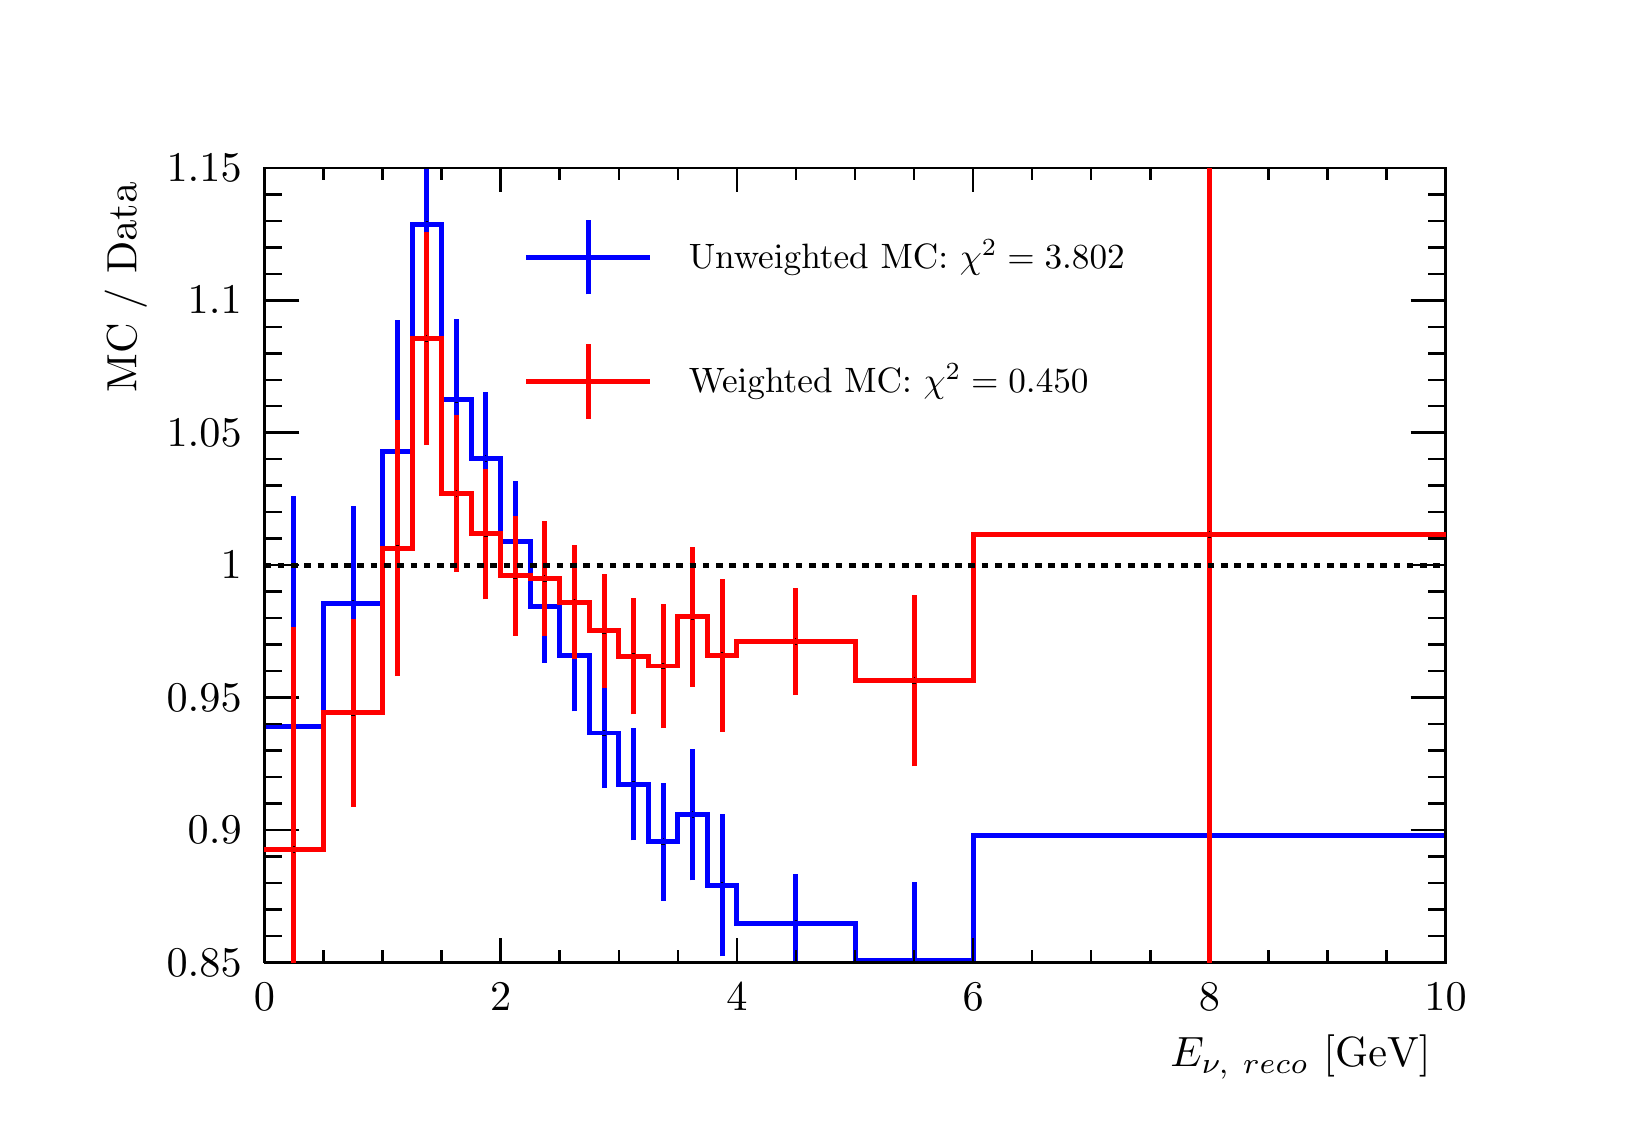
\begin{tikzpicture}
\pgfdeclareplotmark{cross} {
\pgfpathmoveto{\pgfpoint{-0.3\pgfplotmarksize}{\pgfplotmarksize}}
\pgfpathlineto{\pgfpoint{+0.3\pgfplotmarksize}{\pgfplotmarksize}}
\pgfpathlineto{\pgfpoint{+0.3\pgfplotmarksize}{0.3\pgfplotmarksize}}
\pgfpathlineto{\pgfpoint{+1\pgfplotmarksize}{0.3\pgfplotmarksize}}
\pgfpathlineto{\pgfpoint{+1\pgfplotmarksize}{-0.3\pgfplotmarksize}}
\pgfpathlineto{\pgfpoint{+0.3\pgfplotmarksize}{-0.3\pgfplotmarksize}}
\pgfpathlineto{\pgfpoint{+0.3\pgfplotmarksize}{-1.\pgfplotmarksize}}
\pgfpathlineto{\pgfpoint{-0.3\pgfplotmarksize}{-1.\pgfplotmarksize}}
\pgfpathlineto{\pgfpoint{-0.3\pgfplotmarksize}{-0.3\pgfplotmarksize}}
\pgfpathlineto{\pgfpoint{-1.\pgfplotmarksize}{-0.3\pgfplotmarksize}}
\pgfpathlineto{\pgfpoint{-1.\pgfplotmarksize}{0.3\pgfplotmarksize}}
\pgfpathlineto{\pgfpoint{-0.3\pgfplotmarksize}{0.3\pgfplotmarksize}}
\pgfpathclose
\pgfusepathqstroke
}
\pgfdeclareplotmark{cross*} {
\pgfpathmoveto{\pgfpoint{-0.3\pgfplotmarksize}{\pgfplotmarksize}}
\pgfpathlineto{\pgfpoint{+0.3\pgfplotmarksize}{\pgfplotmarksize}}
\pgfpathlineto{\pgfpoint{+0.3\pgfplotmarksize}{0.3\pgfplotmarksize}}
\pgfpathlineto{\pgfpoint{+1\pgfplotmarksize}{0.3\pgfplotmarksize}}
\pgfpathlineto{\pgfpoint{+1\pgfplotmarksize}{-0.3\pgfplotmarksize}}
\pgfpathlineto{\pgfpoint{+0.3\pgfplotmarksize}{-0.3\pgfplotmarksize}}
\pgfpathlineto{\pgfpoint{+0.3\pgfplotmarksize}{-1.\pgfplotmarksize}}
\pgfpathlineto{\pgfpoint{-0.3\pgfplotmarksize}{-1.\pgfplotmarksize}}
\pgfpathlineto{\pgfpoint{-0.3\pgfplotmarksize}{-0.3\pgfplotmarksize}}
\pgfpathlineto{\pgfpoint{-1.\pgfplotmarksize}{-0.3\pgfplotmarksize}}
\pgfpathlineto{\pgfpoint{-1.\pgfplotmarksize}{0.3\pgfplotmarksize}}
\pgfpathlineto{\pgfpoint{-0.3\pgfplotmarksize}{0.3\pgfplotmarksize}}
\pgfpathclose
\pgfusepathqfillstroke
}
\pgfdeclareplotmark{newstar} {
\pgfpathmoveto{\pgfqpoint{0pt}{\pgfplotmarksize}}
\pgfpathlineto{\pgfqpointpolar{44}{0.5\pgfplotmarksize}}
\pgfpathlineto{\pgfqpointpolar{18}{\pgfplotmarksize}}
\pgfpathlineto{\pgfqpointpolar{-20}{0.5\pgfplotmarksize}}
\pgfpathlineto{\pgfqpointpolar{-54}{\pgfplotmarksize}}
\pgfpathlineto{\pgfqpointpolar{-90}{0.5\pgfplotmarksize}}
\pgfpathlineto{\pgfqpointpolar{234}{\pgfplotmarksize}}
\pgfpathlineto{\pgfqpointpolar{198}{0.5\pgfplotmarksize}}
\pgfpathlineto{\pgfqpointpolar{162}{\pgfplotmarksize}}
\pgfpathlineto{\pgfqpointpolar{134}{0.5\pgfplotmarksize}}
\pgfpathclose
\pgfusepathqstroke
}
\pgfdeclareplotmark{newstar*} {
\pgfpathmoveto{\pgfqpoint{0pt}{\pgfplotmarksize}}
\pgfpathlineto{\pgfqpointpolar{44}{0.5\pgfplotmarksize}}
\pgfpathlineto{\pgfqpointpolar{18}{\pgfplotmarksize}}
\pgfpathlineto{\pgfqpointpolar{-20}{0.5\pgfplotmarksize}}
\pgfpathlineto{\pgfqpointpolar{-54}{\pgfplotmarksize}}
\pgfpathlineto{\pgfqpointpolar{-90}{0.5\pgfplotmarksize}}
\pgfpathlineto{\pgfqpointpolar{234}{\pgfplotmarksize}}
\pgfpathlineto{\pgfqpointpolar{198}{0.5\pgfplotmarksize}}
\pgfpathlineto{\pgfqpointpolar{162}{\pgfplotmarksize}}
\pgfpathlineto{\pgfqpointpolar{134}{0.5\pgfplotmarksize}}
\pgfpathclose
\pgfusepathqfillstroke
}
\definecolor{c}{rgb}{1,1,1};
\draw [color=c, fill=c] (0,0) rectangle (20,13.639);
\draw [color=c, fill=c] (3,1.77307) rectangle (18,11.8659);
\definecolor{c}{rgb}{0,0,0};
\draw [c,line width=0.9] (3,1.77307) -- (3,11.8659) -- (18,11.8659) -- (18,1.77307) -- (3,1.77307);
\definecolor{c}{rgb}{1,1,1};
\draw [color=c, fill=c] (3,1.77307) rectangle (18,11.8659);
\definecolor{c}{rgb}{0,0,0};
\draw [c,line width=0.9] (3,1.77307) -- (3,11.8659) -- (18,11.8659) -- (18,1.77307) -- (3,1.77307);
\definecolor{c}{rgb}{0,0,1};
\draw [c,line width=1.8] (3.375,1.8456) -- (3.375,4.77087);
\draw [c,line width=1.8] (3.375,4.77087) -- (3.375,7.69614);
\definecolor{c}{rgb}{0,0,0};
\foreach \P in {(3.375,4.77087)}{\draw[mark options={color=c,fill=c},mark size=2.402402pt, line width=0.000000pt, mark=*,mark size=1pt] plot coordinates {\P};}
\definecolor{c}{rgb}{0,0,1};
\draw [c,line width=1.8] (4.125,5.11119) -- (4.125,6.3386);
\draw [c,line width=1.8] (4.125,6.3386) -- (4.125,7.56602);
\definecolor{c}{rgb}{0,0,0};
\foreach \P in {(4.125,6.3386)}{\draw[mark options={color=c,fill=c},mark size=2.402402pt, line width=0.000000pt, mark=*,mark size=1pt] plot coordinates {\P};}
\definecolor{c}{rgb}{0,0,1};
\draw [c,line width=1.8] (4.6875,6.59132) -- (4.6875,8.2631);
\draw [c,line width=1.8] (4.6875,8.2631) -- (4.6875,9.93489);
\definecolor{c}{rgb}{0,0,0};
\foreach \P in {(4.6875,8.2631)}{\draw[mark options={color=c,fill=c},mark size=2.402402pt, line width=0.000000pt, mark=*,mark size=1pt] plot coordinates {\P};}
\definecolor{c}{rgb}{0,0,1};
\draw [c,line width=1.8] (5.0625,9.76007) -- (5.0625,11.1519);
\draw [c,line width=1.8] (5.0625,11.1519) -- (5.0625,11.8659);
\definecolor{c}{rgb}{0,0,0};
\foreach \P in {(5.0625,11.1519)}{\draw[mark options={color=c,fill=c},mark size=2.402402pt, line width=0.000000pt, mark=*,mark size=1pt] plot coordinates {\P};}
\definecolor{c}{rgb}{0,0,1};
\draw [c,line width=1.8] (5.4375,7.89664) -- (5.4375,8.91997);
\draw [c,line width=1.8] (5.4375,8.91997) -- (5.4375,9.9433);
\definecolor{c}{rgb}{0,0,0};
\foreach \P in {(5.4375,8.91997)}{\draw[mark options={color=c,fill=c},mark size=2.402402pt, line width=0.000000pt, mark=*,mark size=1pt] plot coordinates {\P};}
\definecolor{c}{rgb}{0,0,1};
\draw [c,line width=1.8] (5.8125,7.32529) -- (5.8125,8.17418);
\draw [c,line width=1.8] (5.8125,8.17418) -- (5.8125,9.02306);
\definecolor{c}{rgb}{0,0,0};
\foreach \P in {(5.8125,8.17418)}{\draw[mark options={color=c,fill=c},mark size=2.402402pt, line width=0.000000pt, mark=*,mark size=1pt] plot coordinates {\P};}
\definecolor{c}{rgb}{0,0,1};
\draw [c,line width=1.8] (6.1875,6.34375) -- (6.1875,7.11476);
\draw [c,line width=1.8] (6.1875,7.11476) -- (6.1875,7.88576);
\definecolor{c}{rgb}{0,0,0};
\foreach \P in {(6.1875,7.11476)}{\draw[mark options={color=c,fill=c},mark size=2.402402pt, line width=0.000000pt, mark=*,mark size=1pt] plot coordinates {\P};}
\definecolor{c}{rgb}{0,0,1};
\draw [c,line width=1.8] (6.5625,5.57956) -- (6.5625,6.30079);
\draw [c,line width=1.8] (6.5625,6.30079) -- (6.5625,7.02203);
\definecolor{c}{rgb}{0,0,0};
\foreach \P in {(6.5625,6.30079)}{\draw[mark options={color=c,fill=c},mark size=2.402402pt, line width=0.000000pt, mark=*,mark size=1pt] plot coordinates {\P};}
\definecolor{c}{rgb}{0,0,1};
\draw [c,line width=1.8] (6.9375,4.96311) -- (6.9375,5.67152);
\draw [c,line width=1.8] (6.9375,5.67152) -- (6.9375,6.37993);
\definecolor{c}{rgb}{0,0,0};
\foreach \P in {(6.9375,5.67152)}{\draw[mark options={color=c,fill=c},mark size=2.402402pt, line width=0.000000pt, mark=*,mark size=1pt] plot coordinates {\P};}
\definecolor{c}{rgb}{0,0,1};
\draw [c,line width=1.8] (7.3125,3.98807) -- (7.3125,4.68826);
\draw [c,line width=1.8] (7.3125,4.68826) -- (7.3125,5.38844);
\definecolor{c}{rgb}{0,0,0};
\foreach \P in {(7.3125,4.68826)}{\draw[mark options={color=c,fill=c},mark size=2.402402pt, line width=0.000000pt, mark=*,mark size=1pt] plot coordinates {\P};}
\definecolor{c}{rgb}{0,0,1};
\draw [c,line width=1.8] (7.6875,3.32593) -- (7.6875,4.03969);
\draw [c,line width=1.8] (7.6875,4.03969) -- (7.6875,4.75345);
\definecolor{c}{rgb}{0,0,0};
\foreach \P in {(7.6875,4.03969)}{\draw[mark options={color=c,fill=c},mark size=2.402402pt, line width=0.000000pt, mark=*,mark size=1pt] plot coordinates {\P};}
\definecolor{c}{rgb}{0,0,1};
\draw [c,line width=1.8] (8.0625,2.55826) -- (8.0625,3.30708);
\draw [c,line width=1.8] (8.0625,3.30708) -- (8.0625,4.05591);
\definecolor{c}{rgb}{0,0,0};
\foreach \P in {(8.0625,3.30708)}{\draw[mark options={color=c,fill=c},mark size=2.402402pt, line width=0.000000pt, mark=*,mark size=1pt] plot coordinates {\P};}
\definecolor{c}{rgb}{0,0,1};
\draw [c,line width=1.8] (8.4375,2.81695) -- (8.4375,3.65403);
\draw [c,line width=1.8] (8.4375,3.65403) -- (8.4375,4.4911);
\definecolor{c}{rgb}{0,0,0};
\foreach \P in {(8.4375,3.65403)}{\draw[mark options={color=c,fill=c},mark size=2.402402pt, line width=0.000000pt, mark=*,mark size=1pt] plot coordinates {\P};}
\definecolor{c}{rgb}{0,0,1};
\draw [c,line width=1.8] (8.8125,1.85) -- (8.8125,2.75663);
\draw [c,line width=1.8] (8.8125,2.75663) -- (8.8125,3.66327);
\definecolor{c}{rgb}{0,0,0};
\foreach \P in {(8.8125,2.75663)}{\draw[mark options={color=c,fill=c},mark size=2.402402pt, line width=0.000000pt, mark=*,mark size=1pt] plot coordinates {\P};}
\definecolor{c}{rgb}{0,0,1};
\draw [c,line width=1.8] (9.75,1.77307) -- (9.75,2.27487);
\draw [c,line width=1.8] (9.75,2.27487) -- (9.75,2.89845);
\definecolor{c}{rgb}{0,0,0};
\foreach \P in {(9.75,2.27487)}{\draw[mark options={color=c,fill=c},mark size=2.402402pt, line width=0.000000pt, mark=*,mark size=1pt] plot coordinates {\P};}
\definecolor{c}{rgb}{0,0,1};
\draw [c,line width=1.8] (11.25,1.77307) -- (11.25,1.79527);
\draw [c,line width=1.8] (11.25,1.79527) -- (11.25,2.79368);
\definecolor{c}{rgb}{0,0,0};
\foreach \P in {(11.25,1.79527)}{\draw[mark options={color=c,fill=c},mark size=2.402402pt, line width=0.000000pt, mark=*,mark size=1pt] plot coordinates {\P};}
\definecolor{c}{rgb}{0,0,1};
\draw [c,line width=1.8] (15,1.77307) -- (15,3.38214);
\draw [c,line width=1.8] (15,3.38214) -- (15,11.1883);
\definecolor{c}{rgb}{0,0,0};
\foreach \P in {(15,3.38214)}{\draw[mark options={color=c,fill=c},mark size=2.402402pt, line width=0.000000pt, mark=*,mark size=1pt] plot coordinates {\P};}
\definecolor{c}{rgb}{0,0,1};
\draw [c,line width=1.8] (3,4.77087) -- (3.75,4.77087) -- (3.75,6.3386) -- (4.5,6.3386) -- (4.5,8.2631) -- (4.875,8.2631) -- (4.875,11.1519) -- (5.25,11.1519) -- (5.25,8.91997) -- (5.625,8.91997) -- (5.625,8.17418) -- (6,8.17418) -- (6,7.11476) --
 (6.375,7.11476) -- (6.375,6.30079) -- (6.75,6.30079) -- (6.75,5.67152) -- (7.125,5.67152) -- (7.125,4.68826) -- (7.5,4.68826) -- (7.5,4.03969) -- (7.875,4.03969) -- (7.875,3.30708) -- (8.25,3.30708) -- (8.25,3.65403) -- (8.625,3.65403) --
 (8.625,2.75663) -- (9,2.75663) -- (9,2.27487) -- (10.5,2.27487) -- (10.5,1.79527) -- (12,1.79527) -- (12,3.38214) -- (18,3.38214);
\definecolor{c}{rgb}{0,0,0};
\draw [c,line width=0.9] (3,1.77307) -- (18,1.77307);
\draw [c,line width=0.9] (3,2.07994) -- (3,1.77307);
\draw [c,line width=0.9] (3.75,1.9265) -- (3.75,1.77307);
\draw [c,line width=0.9] (4.5,1.9265) -- (4.5,1.77307);
\draw [c,line width=0.9] (5.25,1.9265) -- (5.25,1.77307);
\draw [c,line width=0.9] (6,2.07994) -- (6,1.77307);
\draw [c,line width=0.9] (6.75,1.9265) -- (6.75,1.77307);
\draw [c,line width=0.9] (7.5,1.9265) -- (7.5,1.77307);
\draw [c,line width=0.9] (8.25,1.9265) -- (8.25,1.77307);
\draw [c,line width=0.9] (9,2.07994) -- (9,1.77307);
\draw [c,line width=0.9] (9.75,1.9265) -- (9.75,1.77307);
\draw [c,line width=0.9] (10.5,1.9265) -- (10.5,1.77307);
\draw [c,line width=0.9] (11.25,1.9265) -- (11.25,1.77307);
\draw [c,line width=0.9] (12,2.07994) -- (12,1.77307);
\draw [c,line width=0.9] (12.75,1.9265) -- (12.75,1.77307);
\draw [c,line width=0.9] (13.5,1.9265) -- (13.5,1.77307);
\draw [c,line width=0.9] (14.25,1.9265) -- (14.25,1.77307);
\draw [c,line width=0.9] (15,2.07994) -- (15,1.77307);
\draw [c,line width=0.9] (15.75,1.9265) -- (15.75,1.77307);
\draw [c,line width=0.9] (16.5,1.9265) -- (16.5,1.77307);
\draw [c,line width=0.9] (17.25,1.9265) -- (17.25,1.77307);
\draw [c,line width=0.9] (18,2.07994) -- (18,1.77307);
\draw [anchor=base] (3,1.15931) node[scale=1.52731, color=c, rotate=0]{0};
\draw [anchor=base] (6,1.15931) node[scale=1.52731, color=c, rotate=0]{2};
\draw [anchor=base] (9,1.15931) node[scale=1.52731, color=c, rotate=0]{4};
\draw [anchor=base] (12,1.15931) node[scale=1.52731, color=c, rotate=0]{6};
\draw [anchor=base] (15,1.15931) node[scale=1.52731, color=c, rotate=0]{8};
\draw [anchor=base] (18,1.15931) node[scale=1.52731, color=c, rotate=0]{10};
\draw [anchor= east] (18,0.572837) node[scale=1.52731, color=c, rotate=0]{$E_{\nu,~\text{reco}}$ [GeV]};
\draw [c,line width=0.9] (3,11.8659) -- (18,11.8659);
\draw [c,line width=0.9] (3,11.559) -- (3,11.8659);
\draw [c,line width=0.9] (3.75,11.7125) -- (3.75,11.8659);
\draw [c,line width=0.9] (4.5,11.7125) -- (4.5,11.8659);
\draw [c,line width=0.9] (5.25,11.7125) -- (5.25,11.8659);
\draw [c,line width=0.9] (6,11.559) -- (6,11.8659);
\draw [c,line width=0.9] (6.75,11.7125) -- (6.75,11.8659);
\draw [c,line width=0.9] (7.5,11.7125) -- (7.5,11.8659);
\draw [c,line width=0.9] (8.25,11.7125) -- (8.25,11.8659);
\draw [c,line width=0.9] (9,11.559) -- (9,11.8659);
\draw [c,line width=0.9] (9.75,11.7125) -- (9.75,11.8659);
\draw [c,line width=0.9] (10.5,11.7125) -- (10.5,11.8659);
\draw [c,line width=0.9] (11.25,11.7125) -- (11.25,11.8659);
\draw [c,line width=0.9] (12,11.559) -- (12,11.8659);
\draw [c,line width=0.9] (12.75,11.7125) -- (12.75,11.8659);
\draw [c,line width=0.9] (13.5,11.7125) -- (13.5,11.8659);
\draw [c,line width=0.9] (14.25,11.7125) -- (14.25,11.8659);
\draw [c,line width=0.9] (15,11.559) -- (15,11.8659);
\draw [c,line width=0.9] (15.75,11.7125) -- (15.75,11.8659);
\draw [c,line width=0.9] (16.5,11.7125) -- (16.5,11.8659);
\draw [c,line width=0.9] (17.25,11.7125) -- (17.25,11.8659);
\draw [c,line width=0.9] (18,11.559) -- (18,11.8659);
\draw [c,line width=0.9] (3,1.77307) -- (3,11.8659);
\draw [c,line width=0.9] (3.444,1.77307) -- (3,1.77307);
\draw [c,line width=0.9] (3.222,2.10949) -- (3,2.10949);
\draw [c,line width=0.9] (3.222,2.44592) -- (3,2.44592);
\draw [c,line width=0.9] (3.222,2.78235) -- (3,2.78235);
\draw [c,line width=0.9] (3.222,3.11878) -- (3,3.11878);
\draw [c,line width=0.9] (3.444,3.45521) -- (3,3.45521);
\draw [c,line width=0.9] (3.222,3.79163) -- (3,3.79163);
\draw [c,line width=0.9] (3.222,4.12806) -- (3,4.12806);
\draw [c,line width=0.9] (3.222,4.46449) -- (3,4.46449);
\draw [c,line width=0.9] (3.222,4.80092) -- (3,4.80092);
\draw [c,line width=0.9] (3.444,5.13734) -- (3,5.13734);
\draw [c,line width=0.9] (3.222,5.47377) -- (3,5.47377);
\draw [c,line width=0.9] (3.222,5.8102) -- (3,5.8102);
\draw [c,line width=0.9] (3.222,6.14663) -- (3,6.14663);
\draw [c,line width=0.9] (3.222,6.48306) -- (3,6.48306);
\draw [c,line width=0.9] (3.444,6.81948) -- (3,6.81948);
\draw [c,line width=0.9] (3.222,7.15591) -- (3,7.15591);
\draw [c,line width=0.9] (3.222,7.49234) -- (3,7.49234);
\draw [c,line width=0.9] (3.222,7.82877) -- (3,7.82877);
\draw [c,line width=0.9] (3.222,8.1652) -- (3,8.1652);
\draw [c,line width=0.9] (3.444,8.50162) -- (3,8.50162);
\draw [c,line width=0.9] (3.222,8.83805) -- (3,8.83805);
\draw [c,line width=0.9] (3.222,9.17448) -- (3,9.17448);
\draw [c,line width=0.9] (3.222,9.51091) -- (3,9.51091);
\draw [c,line width=0.9] (3.222,9.84733) -- (3,9.84733);
\draw [c,line width=0.9] (3.444,10.1838) -- (3,10.1838);
\draw [c,line width=0.9] (3.222,10.5202) -- (3,10.5202);
\draw [c,line width=0.9] (3.222,10.8566) -- (3,10.8566);
\draw [c,line width=0.9] (3.222,11.193) -- (3,11.193);
\draw [c,line width=0.9] (3.222,11.5295) -- (3,11.5295);
\draw [c,line width=0.9] (3.444,11.8659) -- (3,11.8659);
\draw [c,line width=0.9] (3.444,1.77307) -- (3,1.77307);
\draw [c,line width=0.9] (3.444,11.8659) -- (3,11.8659);
\draw [anchor= east] (2.9,1.77307) node[scale=1.52731, color=c, rotate=0]{0.85};
\draw [anchor= east] (2.9,3.45521) node[scale=1.52731, color=c, rotate=0]{0.9};
\draw [anchor= east] (2.9,5.13734) node[scale=1.52731, color=c, rotate=0]{0.95};
\draw [anchor= east] (2.9,6.81948) node[scale=1.52731, color=c, rotate=0]{1};
\draw [anchor= east] (2.9,8.50162) node[scale=1.52731, color=c, rotate=0]{1.05};
\draw [anchor= east] (2.9,10.1838) node[scale=1.52731, color=c, rotate=0]{1.1};
\draw [anchor= east] (2.9,11.8659) node[scale=1.52731, color=c, rotate=0]{1.15};
\draw [anchor= east] (1.24,11.8659) node[scale=1.52731, color=c, rotate=90]{MC / Data};
\draw [c,line width=0.9] (18,1.77307) -- (18,11.8659);
\draw [c,line width=0.9] (17.556,1.77307) -- (18,1.77307);
\draw [c,line width=0.9] (17.778,2.10949) -- (18,2.10949);
\draw [c,line width=0.9] (17.778,2.44592) -- (18,2.44592);
\draw [c,line width=0.9] (17.778,2.78235) -- (18,2.78235);
\draw [c,line width=0.9] (17.778,3.11878) -- (18,3.11878);
\draw [c,line width=0.9] (17.556,3.45521) -- (18,3.45521);
\draw [c,line width=0.9] (17.778,3.79163) -- (18,3.79163);
\draw [c,line width=0.9] (17.778,4.12806) -- (18,4.12806);
\draw [c,line width=0.9] (17.778,4.46449) -- (18,4.46449);
\draw [c,line width=0.9] (17.778,4.80092) -- (18,4.80092);
\draw [c,line width=0.9] (17.556,5.13734) -- (18,5.13734);
\draw [c,line width=0.9] (17.778,5.47377) -- (18,5.47377);
\draw [c,line width=0.9] (17.778,5.8102) -- (18,5.8102);
\draw [c,line width=0.9] (17.778,6.14663) -- (18,6.14663);
\draw [c,line width=0.9] (17.778,6.48306) -- (18,6.48306);
\draw [c,line width=0.9] (17.556,6.81948) -- (18,6.81948);
\draw [c,line width=0.9] (17.778,7.15591) -- (18,7.15591);
\draw [c,line width=0.9] (17.778,7.49234) -- (18,7.49234);
\draw [c,line width=0.9] (17.778,7.82877) -- (18,7.82877);
\draw [c,line width=0.9] (17.778,8.1652) -- (18,8.1652);
\draw [c,line width=0.9] (17.556,8.50162) -- (18,8.50162);
\draw [c,line width=0.9] (17.778,8.83805) -- (18,8.83805);
\draw [c,line width=0.9] (17.778,9.17448) -- (18,9.17448);
\draw [c,line width=0.9] (17.778,9.51091) -- (18,9.51091);
\draw [c,line width=0.9] (17.778,9.84733) -- (18,9.84733);
\draw [c,line width=0.9] (17.556,10.1838) -- (18,10.1838);
\draw [c,line width=0.9] (17.778,10.5202) -- (18,10.5202);
\draw [c,line width=0.9] (17.778,10.8566) -- (18,10.8566);
\draw [c,line width=0.9] (17.778,11.193) -- (18,11.193);
\draw [c,line width=0.9] (17.778,11.5295) -- (18,11.5295);
\draw [c,line width=0.9] (17.556,11.8659) -- (18,11.8659);
\draw [c,line width=0.9] (17.556,1.77307) -- (18,1.77307);
\draw [c,line width=0.9] (17.556,11.8659) -- (18,11.8659);
\definecolor{c}{rgb}{1,0,0};
\draw [c,line width=1.8] (3.375,1.77307) -- (3.375,3.21093);
\draw [c,line width=1.8] (3.375,3.21093) -- (3.375,6.02876);
\definecolor{c}{rgb}{0,0,0};
\foreach \P in {(3.375,3.21093)}{\draw[mark options={color=c,fill=c},mark size=2.402402pt, line width=0.000000pt, mark=*,mark size=1pt] plot coordinates {\P};}
\definecolor{c}{rgb}{1,0,0};
\draw [c,line width=1.8] (4.125,3.75466) -- (4.125,4.94337);
\draw [c,line width=1.8] (4.125,4.94337) -- (4.125,6.13207);
\definecolor{c}{rgb}{0,0,0};
\foreach \P in {(4.125,4.94337)}{\draw[mark options={color=c,fill=c},mark size=2.402402pt, line width=0.000000pt, mark=*,mark size=1pt] plot coordinates {\P};}
\definecolor{c}{rgb}{1,0,0};
\draw [c,line width=1.8] (4.6875,5.40974) -- (4.6875,7.03735);
\draw [c,line width=1.8] (4.6875,7.03735) -- (4.6875,8.66497);
\definecolor{c}{rgb}{0,0,0};
\foreach \P in {(4.6875,7.03735)}{\draw[mark options={color=c,fill=c},mark size=2.402402pt, line width=0.000000pt, mark=*,mark size=1pt] plot coordinates {\P};}
\definecolor{c}{rgb}{1,0,0};
\draw [c,line width=1.8] (5.0625,8.34554) -- (5.0625,9.69648);
\draw [c,line width=1.8] (5.0625,9.69648) -- (5.0625,11.0474);
\definecolor{c}{rgb}{0,0,0};
\foreach \P in {(5.0625,9.69648)}{\draw[mark options={color=c,fill=c},mark size=2.402402pt, line width=0.000000pt, mark=*,mark size=1pt] plot coordinates {\P};}
\definecolor{c}{rgb}{1,0,0};
\draw [c,line width=1.8] (5.4375,6.73558) -- (5.4375,7.73313);
\draw [c,line width=1.8] (5.4375,7.73313) -- (5.4375,8.73069);
\definecolor{c}{rgb}{0,0,0};
\foreach \P in {(5.4375,7.73313)}{\draw[mark options={color=c,fill=c},mark size=2.402402pt, line width=0.000000pt, mark=*,mark size=1pt] plot coordinates {\P};}
\definecolor{c}{rgb}{1,0,0};
\draw [c,line width=1.8] (5.8125,6.38464) -- (5.8125,7.21596);
\draw [c,line width=1.8] (5.8125,7.21596) -- (5.8125,8.04728);
\definecolor{c}{rgb}{0,0,0};
\foreach \P in {(5.8125,7.21596)}{\draw[mark options={color=c,fill=c},mark size=2.402402pt, line width=0.000000pt, mark=*,mark size=1pt] plot coordinates {\P};}
\definecolor{c}{rgb}{1,0,0};
\draw [c,line width=1.8] (6.1875,5.92048) -- (6.1875,6.68413);
\draw [c,line width=1.8] (6.1875,6.68413) -- (6.1875,7.44777);
\definecolor{c}{rgb}{0,0,0};
\foreach \P in {(6.1875,6.68413)}{\draw[mark options={color=c,fill=c},mark size=2.402402pt, line width=0.000000pt, mark=*,mark size=1pt] plot coordinates {\P};}
\definecolor{c}{rgb}{1,0,0};
\draw [c,line width=1.8] (6.5625,5.92148) -- (6.5625,6.64838);
\draw [c,line width=1.8] (6.5625,6.64838) -- (6.5625,7.37527);
\definecolor{c}{rgb}{0,0,0};
\foreach \P in {(6.5625,6.64838)}{\draw[mark options={color=c,fill=c},mark size=2.402402pt, line width=0.000000pt, mark=*,mark size=1pt] plot coordinates {\P};}
\definecolor{c}{rgb}{1,0,0};
\draw [c,line width=1.8] (6.9375,5.63069) -- (6.9375,6.35012);
\draw [c,line width=1.8] (6.9375,6.35012) -- (6.9375,7.06955);
\definecolor{c}{rgb}{0,0,0};
\foreach \P in {(6.9375,6.35012)}{\draw[mark options={color=c,fill=c},mark size=2.402402pt, line width=0.000000pt, mark=*,mark size=1pt] plot coordinates {\P};}
\definecolor{c}{rgb}{1,0,0};
\draw [c,line width=1.8] (7.3125,5.26357) -- (7.3125,5.9851);
\draw [c,line width=1.8] (7.3125,5.9851) -- (7.3125,6.70663);
\definecolor{c}{rgb}{0,0,0};
\foreach \P in {(7.3125,5.9851)}{\draw[mark options={color=c,fill=c},mark size=2.402402pt, line width=0.000000pt, mark=*,mark size=1pt] plot coordinates {\P};}
\definecolor{c}{rgb}{1,0,0};
\draw [c,line width=1.8] (7.6875,4.92425) -- (7.6875,5.66574);
\draw [c,line width=1.8] (7.6875,5.66574) -- (7.6875,6.40724);
\definecolor{c}{rgb}{0,0,0};
\foreach \P in {(7.6875,5.66574)}{\draw[mark options={color=c,fill=c},mark size=2.402402pt, line width=0.000000pt, mark=*,mark size=1pt] plot coordinates {\P};}
\definecolor{c}{rgb}{1,0,0};
\draw [c,line width=1.8] (8.0625,4.74969) -- (8.0625,5.53923);
\draw [c,line width=1.8] (8.0625,5.53923) -- (8.0625,6.32876);
\definecolor{c}{rgb}{0,0,0};
\foreach \P in {(8.0625,5.53923)}{\draw[mark options={color=c,fill=c},mark size=2.402402pt, line width=0.000000pt, mark=*,mark size=1pt] plot coordinates {\P};}
\definecolor{c}{rgb}{1,0,0};
\draw [c,line width=1.8] (8.4375,5.27621) -- (8.4375,6.16396);
\draw [c,line width=1.8] (8.4375,6.16396) -- (8.4375,7.0517);
\definecolor{c}{rgb}{0,0,0};
\foreach \P in {(8.4375,6.16396)}{\draw[mark options={color=c,fill=c},mark size=2.402402pt, line width=0.000000pt, mark=*,mark size=1pt] plot coordinates {\P};}
\definecolor{c}{rgb}{1,0,0};
\draw [c,line width=1.8] (8.8125,4.70509) -- (8.8125,5.67713);
\draw [c,line width=1.8] (8.8125,5.67713) -- (8.8125,6.64917);
\definecolor{c}{rgb}{0,0,0};
\foreach \P in {(8.8125,5.67713)}{\draw[mark options={color=c,fill=c},mark size=2.402402pt, line width=0.000000pt, mark=*,mark size=1pt] plot coordinates {\P};}
\definecolor{c}{rgb}{1,0,0};
\draw [c,line width=1.8] (9.75,5.17003) -- (9.75,5.84937);
\draw [c,line width=1.8] (9.75,5.84937) -- (9.75,6.52871);
\definecolor{c}{rgb}{0,0,0};
\foreach \P in {(9.75,5.84937)}{\draw[mark options={color=c,fill=c},mark size=2.402402pt, line width=0.000000pt, mark=*,mark size=1pt] plot coordinates {\P};}
\definecolor{c}{rgb}{1,0,0};
\draw [c,line width=1.8] (11.25,4.26381) -- (11.25,5.35227);
\draw [c,line width=1.8] (11.25,5.35227) -- (11.25,6.44074);
\definecolor{c}{rgb}{0,0,0};
\foreach \P in {(11.25,5.35227)}{\draw[mark options={color=c,fill=c},mark size=2.402402pt, line width=0.000000pt, mark=*,mark size=1pt] plot coordinates {\P};}
\definecolor{c}{rgb}{1,0,0};
\draw [c,line width=1.8] (15,1.77307) -- (15,7.20907);
\draw [c,line width=1.8] (15,7.20907) -- (15,11.8659);
\definecolor{c}{rgb}{0,0,0};
\foreach \P in {(15,7.20907)}{\draw[mark options={color=c,fill=c},mark size=2.402402pt, line width=0.000000pt, mark=*,mark size=1pt] plot coordinates {\P};}
\definecolor{c}{rgb}{1,0,0};
\draw [c,line width=1.8] (3,3.21093) -- (3.75,3.21093) -- (3.75,4.94337) -- (4.5,4.94337) -- (4.5,7.03735) -- (4.875,7.03735) -- (4.875,9.69648) -- (5.25,9.69648) -- (5.25,7.73313) -- (5.625,7.73313) -- (5.625,7.21596) -- (6,7.21596) -- (6,6.68413)
 -- (6.375,6.68413) -- (6.375,6.64838) -- (6.75,6.64838) -- (6.75,6.35012) -- (7.125,6.35012) -- (7.125,5.9851) -- (7.5,5.9851) -- (7.5,5.66574) -- (7.875,5.66574) -- (7.875,5.53923) -- (8.25,5.53923) -- (8.25,6.16396) -- (8.625,6.16396) --
 (8.625,5.67713) -- (9,5.67713) -- (9,5.84937) -- (10.5,5.84937) -- (10.5,5.35227) -- (12,5.35227) -- (12,7.20907) -- (18,7.20907);
\definecolor{c}{rgb}{0,0,0};
\draw [c,dash pattern=on 2.40pt off 2.40pt ,line width=1.8] (3,6.81948) -- (18,6.81948);
\definecolor{c}{rgb}{1,1,1};
\draw [color=c, fill=c] (5.98854,8.36676) rectangle (14.957,11.5186);
\definecolor{c}{rgb}{0,0,0};
\draw [anchor= west] (8.23066,10.7307) node[scale=1.27276, color=c, rotate=0]{Unweighted MC: $\chi^{2} = 3.802$};
\definecolor{c}{rgb}{0,0,1};
\draw [c,line width=1.8] (6.32486,10.7307) -- (7.89434,10.7307);
\draw [c,line width=1.8] (7.1096,10.2579) -- (7.1096,11.2034);
\definecolor{c}{rgb}{0,0,0};
\draw [anchor= west] (8.23066,9.15473) node[scale=1.27276, color=c, rotate=0]{Weighted MC: $\chi^{2} = 0.450$};
\definecolor{c}{rgb}{1,0,0};
\draw [c,line width=1.8] (6.32486,9.15473) -- (7.89434,9.15473);
\draw [c,line width=1.8] (7.1096,8.68195) -- (7.1096,9.62751);
\definecolor{c}{rgb}{1,1,1};
\draw [color=c, fill=c] (2,12.8206) rectangle (18,13.5708);
\end{tikzpicture}

		\end{adjustbox}
		\caption{FHC \nue}
	\end{subfigure} \\
	\begin{subfigure}[t]{.5\linewidth}
		\begin{adjustbox}{max totalsize=\linewidth, center}
			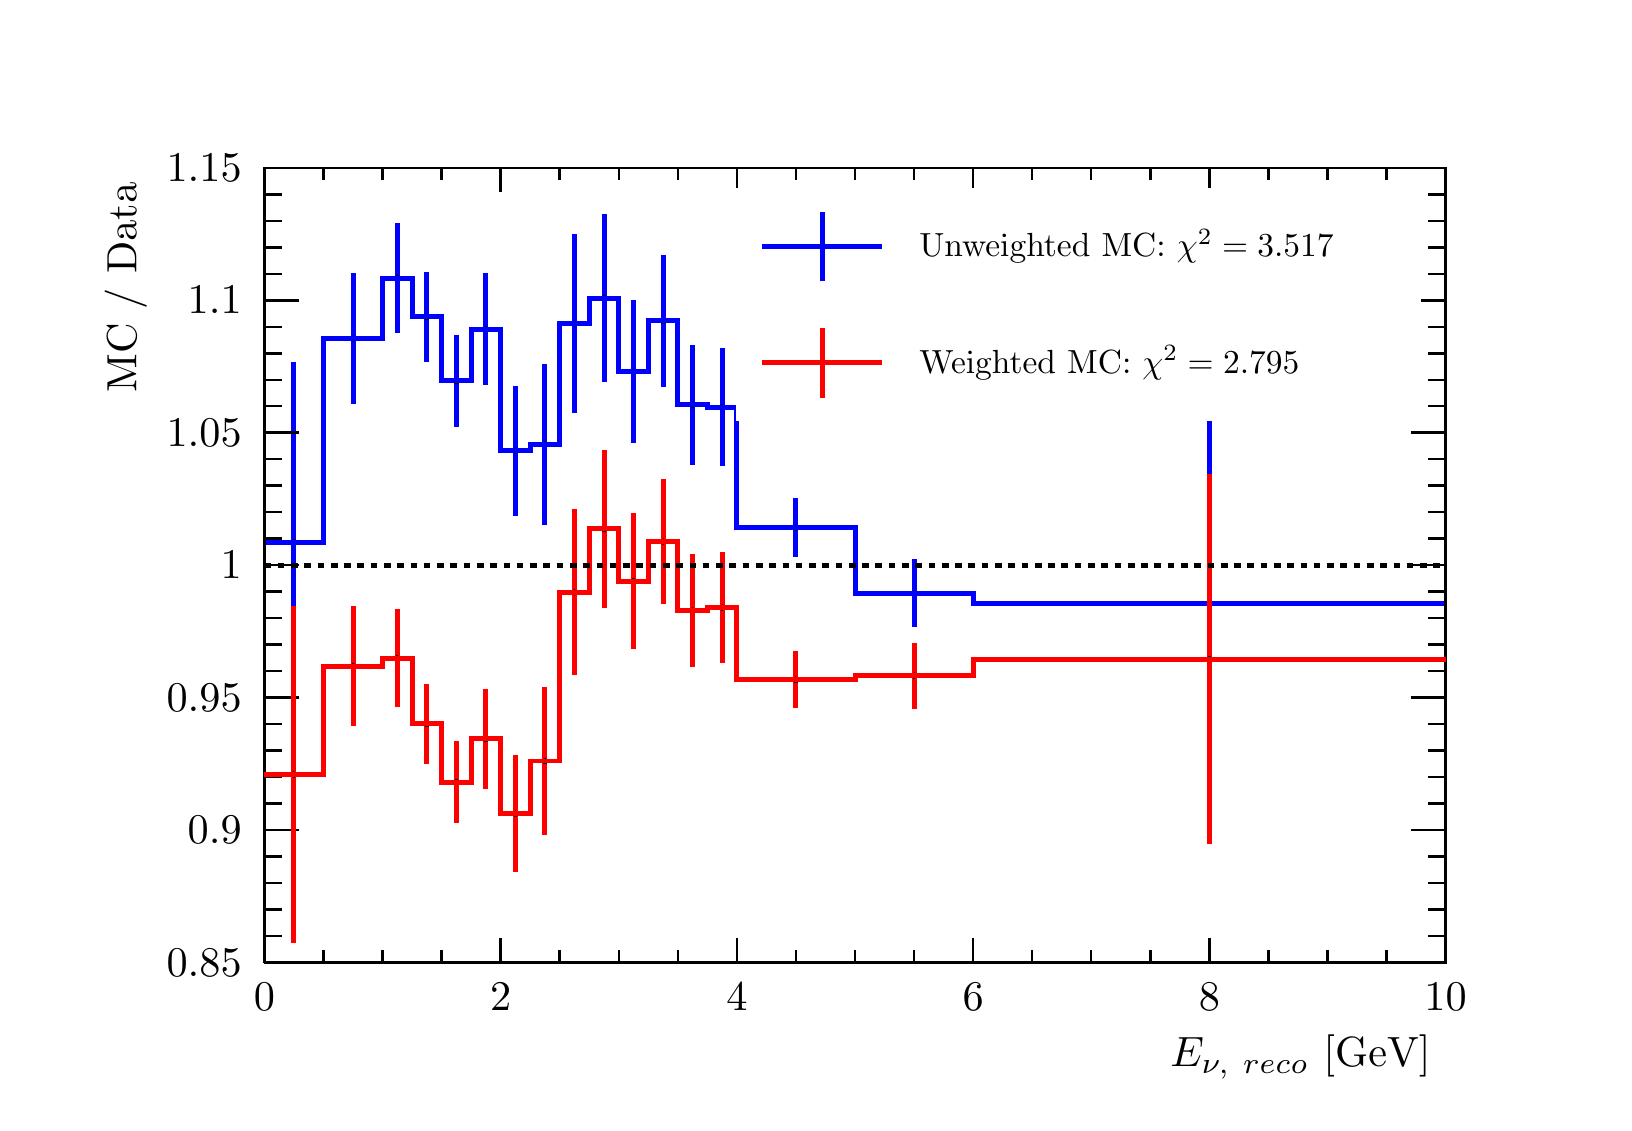
\begin{tikzpicture}
\pgfdeclareplotmark{cross} {
\pgfpathmoveto{\pgfpoint{-0.3\pgfplotmarksize}{\pgfplotmarksize}}
\pgfpathlineto{\pgfpoint{+0.3\pgfplotmarksize}{\pgfplotmarksize}}
\pgfpathlineto{\pgfpoint{+0.3\pgfplotmarksize}{0.3\pgfplotmarksize}}
\pgfpathlineto{\pgfpoint{+1\pgfplotmarksize}{0.3\pgfplotmarksize}}
\pgfpathlineto{\pgfpoint{+1\pgfplotmarksize}{-0.3\pgfplotmarksize}}
\pgfpathlineto{\pgfpoint{+0.3\pgfplotmarksize}{-0.3\pgfplotmarksize}}
\pgfpathlineto{\pgfpoint{+0.3\pgfplotmarksize}{-1.\pgfplotmarksize}}
\pgfpathlineto{\pgfpoint{-0.3\pgfplotmarksize}{-1.\pgfplotmarksize}}
\pgfpathlineto{\pgfpoint{-0.3\pgfplotmarksize}{-0.3\pgfplotmarksize}}
\pgfpathlineto{\pgfpoint{-1.\pgfplotmarksize}{-0.3\pgfplotmarksize}}
\pgfpathlineto{\pgfpoint{-1.\pgfplotmarksize}{0.3\pgfplotmarksize}}
\pgfpathlineto{\pgfpoint{-0.3\pgfplotmarksize}{0.3\pgfplotmarksize}}
\pgfpathclose
\pgfusepathqstroke
}
\pgfdeclareplotmark{cross*} {
\pgfpathmoveto{\pgfpoint{-0.3\pgfplotmarksize}{\pgfplotmarksize}}
\pgfpathlineto{\pgfpoint{+0.3\pgfplotmarksize}{\pgfplotmarksize}}
\pgfpathlineto{\pgfpoint{+0.3\pgfplotmarksize}{0.3\pgfplotmarksize}}
\pgfpathlineto{\pgfpoint{+1\pgfplotmarksize}{0.3\pgfplotmarksize}}
\pgfpathlineto{\pgfpoint{+1\pgfplotmarksize}{-0.3\pgfplotmarksize}}
\pgfpathlineto{\pgfpoint{+0.3\pgfplotmarksize}{-0.3\pgfplotmarksize}}
\pgfpathlineto{\pgfpoint{+0.3\pgfplotmarksize}{-1.\pgfplotmarksize}}
\pgfpathlineto{\pgfpoint{-0.3\pgfplotmarksize}{-1.\pgfplotmarksize}}
\pgfpathlineto{\pgfpoint{-0.3\pgfplotmarksize}{-0.3\pgfplotmarksize}}
\pgfpathlineto{\pgfpoint{-1.\pgfplotmarksize}{-0.3\pgfplotmarksize}}
\pgfpathlineto{\pgfpoint{-1.\pgfplotmarksize}{0.3\pgfplotmarksize}}
\pgfpathlineto{\pgfpoint{-0.3\pgfplotmarksize}{0.3\pgfplotmarksize}}
\pgfpathclose
\pgfusepathqfillstroke
}
\pgfdeclareplotmark{newstar} {
\pgfpathmoveto{\pgfqpoint{0pt}{\pgfplotmarksize}}
\pgfpathlineto{\pgfqpointpolar{44}{0.5\pgfplotmarksize}}
\pgfpathlineto{\pgfqpointpolar{18}{\pgfplotmarksize}}
\pgfpathlineto{\pgfqpointpolar{-20}{0.5\pgfplotmarksize}}
\pgfpathlineto{\pgfqpointpolar{-54}{\pgfplotmarksize}}
\pgfpathlineto{\pgfqpointpolar{-90}{0.5\pgfplotmarksize}}
\pgfpathlineto{\pgfqpointpolar{234}{\pgfplotmarksize}}
\pgfpathlineto{\pgfqpointpolar{198}{0.5\pgfplotmarksize}}
\pgfpathlineto{\pgfqpointpolar{162}{\pgfplotmarksize}}
\pgfpathlineto{\pgfqpointpolar{134}{0.5\pgfplotmarksize}}
\pgfpathclose
\pgfusepathqstroke
}
\pgfdeclareplotmark{newstar*} {
\pgfpathmoveto{\pgfqpoint{0pt}{\pgfplotmarksize}}
\pgfpathlineto{\pgfqpointpolar{44}{0.5\pgfplotmarksize}}
\pgfpathlineto{\pgfqpointpolar{18}{\pgfplotmarksize}}
\pgfpathlineto{\pgfqpointpolar{-20}{0.5\pgfplotmarksize}}
\pgfpathlineto{\pgfqpointpolar{-54}{\pgfplotmarksize}}
\pgfpathlineto{\pgfqpointpolar{-90}{0.5\pgfplotmarksize}}
\pgfpathlineto{\pgfqpointpolar{234}{\pgfplotmarksize}}
\pgfpathlineto{\pgfqpointpolar{198}{0.5\pgfplotmarksize}}
\pgfpathlineto{\pgfqpointpolar{162}{\pgfplotmarksize}}
\pgfpathlineto{\pgfqpointpolar{134}{0.5\pgfplotmarksize}}
\pgfpathclose
\pgfusepathqfillstroke
}
\definecolor{c}{rgb}{1,1,1};
\draw [color=c, fill=c] (0,0) rectangle (20,13.639);
\draw [color=c, fill=c] (3,1.77307) rectangle (18,11.8659);
\definecolor{c}{rgb}{0,0,0};
\draw [c,line width=0.9] (3,1.77307) -- (3,11.8659) -- (18,11.8659) -- (18,1.77307) -- (3,1.77307);
\definecolor{c}{rgb}{1,1,1};
\draw [color=c, fill=c] (3,1.77307) rectangle (18,11.8659);
\definecolor{c}{rgb}{0,0,0};
\draw [c,line width=0.9] (3,1.77307) -- (3,11.8659) -- (18,11.8659) -- (18,1.77307) -- (3,1.77307);
\definecolor{c}{rgb}{0,0,1};
\draw [c,line width=1.8] (3.375,4.82235) -- (3.375,7.11133);
\draw [c,line width=1.8] (3.375,7.11133) -- (3.375,9.4003);
\definecolor{c}{rgb}{0,0,0};
\foreach \P in {(3.375,7.11133)}{\draw[mark options={color=c,fill=c},mark size=2.402402pt, line width=0.000000pt, mark=*,mark size=1pt] plot coordinates {\P};}
\definecolor{c}{rgb}{0,0,1};
\draw [c,line width=1.8] (4.125,8.86415) -- (4.125,9.69792);
\draw [c,line width=1.8] (4.125,9.69792) -- (4.125,10.5317);
\definecolor{c}{rgb}{0,0,0};
\foreach \P in {(4.125,9.69792)}{\draw[mark options={color=c,fill=c},mark size=2.402402pt, line width=0.000000pt, mark=*,mark size=1pt] plot coordinates {\P};}
\definecolor{c}{rgb}{0,0,1};
\draw [c,line width=1.8] (4.6875,9.77105) -- (4.6875,10.4651);
\draw [c,line width=1.8] (4.6875,10.4651) -- (4.6875,11.1591);
\definecolor{c}{rgb}{0,0,0};
\foreach \P in {(4.6875,10.4651)}{\draw[mark options={color=c,fill=c},mark size=2.402402pt, line width=0.000000pt, mark=*,mark size=1pt] plot coordinates {\P};}
\definecolor{c}{rgb}{0,0,1};
\draw [c,line width=1.8] (5.0625,9.40033) -- (5.0625,9.97166);
\draw [c,line width=1.8] (5.0625,9.97166) -- (5.0625,10.543);
\definecolor{c}{rgb}{0,0,0};
\foreach \P in {(5.0625,9.97166)}{\draw[mark options={color=c,fill=c},mark size=2.402402pt, line width=0.000000pt, mark=*,mark size=1pt] plot coordinates {\P};}
\definecolor{c}{rgb}{0,0,1};
\draw [c,line width=1.8] (5.4375,8.57753) -- (5.4375,9.1589);
\draw [c,line width=1.8] (5.4375,9.1589) -- (5.4375,9.74027);
\definecolor{c}{rgb}{0,0,0};
\foreach \P in {(5.4375,9.1589)}{\draw[mark options={color=c,fill=c},mark size=2.402402pt, line width=0.000000pt, mark=*,mark size=1pt] plot coordinates {\P};}
\definecolor{c}{rgb}{0,0,1};
\draw [c,line width=1.8] (5.8125,9.11223) -- (5.8125,9.81875);
\draw [c,line width=1.8] (5.8125,9.81875) -- (5.8125,10.5253);
\definecolor{c}{rgb}{0,0,0};
\foreach \P in {(5.8125,9.81875)}{\draw[mark options={color=c,fill=c},mark size=2.402402pt, line width=0.000000pt, mark=*,mark size=1pt] plot coordinates {\P};}
\definecolor{c}{rgb}{0,0,1};
\draw [c,line width=1.8] (6.1875,7.4464) -- (6.1875,8.27347);
\draw [c,line width=1.8] (6.1875,8.27347) -- (6.1875,9.10054);
\definecolor{c}{rgb}{0,0,0};
\foreach \P in {(6.1875,8.27347)}{\draw[mark options={color=c,fill=c},mark size=2.402402pt, line width=0.000000pt, mark=*,mark size=1pt] plot coordinates {\P};}
\definecolor{c}{rgb}{0,0,1};
\draw [c,line width=1.8] (6.5625,7.3329) -- (6.5625,8.35608);
\draw [c,line width=1.8] (6.5625,8.35608) -- (6.5625,9.37926);
\definecolor{c}{rgb}{0,0,0};
\foreach \P in {(6.5625,8.35608)}{\draw[mark options={color=c,fill=c},mark size=2.402402pt, line width=0.000000pt, mark=*,mark size=1pt] plot coordinates {\P};}
\definecolor{c}{rgb}{0,0,1};
\draw [c,line width=1.8] (6.9375,8.75536) -- (6.9375,9.89207);
\draw [c,line width=1.8] (6.9375,9.89207) -- (6.9375,11.0288);
\definecolor{c}{rgb}{0,0,0};
\foreach \P in {(6.9375,9.89207)}{\draw[mark options={color=c,fill=c},mark size=2.402402pt, line width=0.000000pt, mark=*,mark size=1pt] plot coordinates {\P};}
\definecolor{c}{rgb}{0,0,1};
\draw [c,line width=1.8] (7.3125,9.14294) -- (7.3125,10.2107);
\draw [c,line width=1.8] (7.3125,10.2107) -- (7.3125,11.2785);
\definecolor{c}{rgb}{0,0,0};
\foreach \P in {(7.3125,10.2107)}{\draw[mark options={color=c,fill=c},mark size=2.402402pt, line width=0.000000pt, mark=*,mark size=1pt] plot coordinates {\P};}
\definecolor{c}{rgb}{0,0,1};
\draw [c,line width=1.8] (7.6875,8.37385) -- (7.6875,9.28303);
\draw [c,line width=1.8] (7.6875,9.28303) -- (7.6875,10.1922);
\definecolor{c}{rgb}{0,0,0};
\foreach \P in {(7.6875,9.28303)}{\draw[mark options={color=c,fill=c},mark size=2.402402pt, line width=0.000000pt, mark=*,mark size=1pt] plot coordinates {\P};}
\definecolor{c}{rgb}{0,0,1};
\draw [c,line width=1.8] (8.0625,9.08244) -- (8.0625,9.92258);
\draw [c,line width=1.8] (8.0625,9.92258) -- (8.0625,10.7627);
\definecolor{c}{rgb}{0,0,0};
\foreach \P in {(8.0625,9.92258)}{\draw[mark options={color=c,fill=c},mark size=2.402402pt, line width=0.000000pt, mark=*,mark size=1pt] plot coordinates {\P};}
\definecolor{c}{rgb}{0,0,1};
\draw [c,line width=1.8] (8.4375,8.09525) -- (8.4375,8.85714);
\draw [c,line width=1.8] (8.4375,8.85714) -- (8.4375,9.61902);
\definecolor{c}{rgb}{0,0,0};
\foreach \P in {(8.4375,8.85714)}{\draw[mark options={color=c,fill=c},mark size=2.402402pt, line width=0.000000pt, mark=*,mark size=1pt] plot coordinates {\P};}
\definecolor{c}{rgb}{0,0,1};
\draw [c,line width=1.8] (8.8125,8.07856) -- (8.8125,8.82826);
\draw [c,line width=1.8] (8.8125,8.82826) -- (8.8125,9.57796);
\definecolor{c}{rgb}{0,0,0};
\foreach \P in {(8.8125,8.82826)}{\draw[mark options={color=c,fill=c},mark size=2.402402pt, line width=0.000000pt, mark=*,mark size=1pt] plot coordinates {\P};}
\definecolor{c}{rgb}{0,0,1};
\draw [c,line width=1.8] (9.75,6.92167) -- (9.75,7.29785);
\draw [c,line width=1.8] (9.75,7.29785) -- (9.75,7.67403);
\definecolor{c}{rgb}{0,0,0};
\foreach \P in {(9.75,7.29785)}{\draw[mark options={color=c,fill=c},mark size=2.402402pt, line width=0.000000pt, mark=*,mark size=1pt] plot coordinates {\P};}
\definecolor{c}{rgb}{0,0,1};
\draw [c,line width=1.8] (11.25,6.03502) -- (11.25,6.46348);
\draw [c,line width=1.8] (11.25,6.46348) -- (11.25,6.89195);
\definecolor{c}{rgb}{0,0,0};
\foreach \P in {(11.25,6.46348)}{\draw[mark options={color=c,fill=c},mark size=2.402402pt, line width=0.000000pt, mark=*,mark size=1pt] plot coordinates {\P};}
\definecolor{c}{rgb}{0,0,1};
\draw [c,line width=1.8] (15,3.94313) -- (15,6.32831);
\draw [c,line width=1.8] (15,6.32831) -- (15,8.71348);
\definecolor{c}{rgb}{0,0,0};
\foreach \P in {(15,6.32831)}{\draw[mark options={color=c,fill=c},mark size=2.402402pt, line width=0.000000pt, mark=*,mark size=1pt] plot coordinates {\P};}
\definecolor{c}{rgb}{0,0,1};
\draw [c,line width=1.8] (3,7.11133) -- (3.75,7.11133) -- (3.75,9.69792) -- (4.5,9.69792) -- (4.5,10.4651) -- (4.875,10.4651) -- (4.875,9.97166) -- (5.25,9.97166) -- (5.25,9.1589) -- (5.625,9.1589) -- (5.625,9.81875) -- (6,9.81875) -- (6,8.27347) --
 (6.375,8.27347) -- (6.375,8.35608) -- (6.75,8.35608) -- (6.75,9.89207) -- (7.125,9.89207) -- (7.125,10.2107) -- (7.5,10.2107) -- (7.5,9.28303) -- (7.875,9.28303) -- (7.875,9.92258) -- (8.25,9.92258) -- (8.25,8.85714) -- (8.625,8.85714) --
 (8.625,8.82826) -- (9,8.82826) -- (9,7.29785) -- (10.5,7.29785) -- (10.5,6.46348) -- (12,6.46348) -- (12,6.32831) -- (18,6.32831);
\definecolor{c}{rgb}{0,0,0};
\draw [c,line width=0.9] (3,1.77307) -- (18,1.77307);
\draw [c,line width=0.9] (3,2.07994) -- (3,1.77307);
\draw [c,line width=0.9] (3.75,1.9265) -- (3.75,1.77307);
\draw [c,line width=0.9] (4.5,1.9265) -- (4.5,1.77307);
\draw [c,line width=0.9] (5.25,1.9265) -- (5.25,1.77307);
\draw [c,line width=0.9] (6,2.07994) -- (6,1.77307);
\draw [c,line width=0.9] (6.75,1.9265) -- (6.75,1.77307);
\draw [c,line width=0.9] (7.5,1.9265) -- (7.5,1.77307);
\draw [c,line width=0.9] (8.25,1.9265) -- (8.25,1.77307);
\draw [c,line width=0.9] (9,2.07994) -- (9,1.77307);
\draw [c,line width=0.9] (9.75,1.9265) -- (9.75,1.77307);
\draw [c,line width=0.9] (10.5,1.9265) -- (10.5,1.77307);
\draw [c,line width=0.9] (11.25,1.9265) -- (11.25,1.77307);
\draw [c,line width=0.9] (12,2.07994) -- (12,1.77307);
\draw [c,line width=0.9] (12.75,1.9265) -- (12.75,1.77307);
\draw [c,line width=0.9] (13.5,1.9265) -- (13.5,1.77307);
\draw [c,line width=0.9] (14.25,1.9265) -- (14.25,1.77307);
\draw [c,line width=0.9] (15,2.07994) -- (15,1.77307);
\draw [c,line width=0.9] (15.75,1.9265) -- (15.75,1.77307);
\draw [c,line width=0.9] (16.5,1.9265) -- (16.5,1.77307);
\draw [c,line width=0.9] (17.25,1.9265) -- (17.25,1.77307);
\draw [c,line width=0.9] (18,2.07994) -- (18,1.77307);
\draw [anchor=base] (3,1.15931) node[scale=1.52731, color=c, rotate=0]{0};
\draw [anchor=base] (6,1.15931) node[scale=1.52731, color=c, rotate=0]{2};
\draw [anchor=base] (9,1.15931) node[scale=1.52731, color=c, rotate=0]{4};
\draw [anchor=base] (12,1.15931) node[scale=1.52731, color=c, rotate=0]{6};
\draw [anchor=base] (15,1.15931) node[scale=1.52731, color=c, rotate=0]{8};
\draw [anchor=base] (18,1.15931) node[scale=1.52731, color=c, rotate=0]{10};
\draw [anchor= east] (18,0.572837) node[scale=1.52731, color=c, rotate=0]{$E_{\nu,~\text{reco}}$ [GeV]};
\draw [c,line width=0.9] (3,11.8659) -- (18,11.8659);
\draw [c,line width=0.9] (3,11.559) -- (3,11.8659);
\draw [c,line width=0.9] (3.75,11.7125) -- (3.75,11.8659);
\draw [c,line width=0.9] (4.5,11.7125) -- (4.5,11.8659);
\draw [c,line width=0.9] (5.25,11.7125) -- (5.25,11.8659);
\draw [c,line width=0.9] (6,11.559) -- (6,11.8659);
\draw [c,line width=0.9] (6.75,11.7125) -- (6.75,11.8659);
\draw [c,line width=0.9] (7.5,11.7125) -- (7.5,11.8659);
\draw [c,line width=0.9] (8.25,11.7125) -- (8.25,11.8659);
\draw [c,line width=0.9] (9,11.559) -- (9,11.8659);
\draw [c,line width=0.9] (9.75,11.7125) -- (9.75,11.8659);
\draw [c,line width=0.9] (10.5,11.7125) -- (10.5,11.8659);
\draw [c,line width=0.9] (11.25,11.7125) -- (11.25,11.8659);
\draw [c,line width=0.9] (12,11.559) -- (12,11.8659);
\draw [c,line width=0.9] (12.75,11.7125) -- (12.75,11.8659);
\draw [c,line width=0.9] (13.5,11.7125) -- (13.5,11.8659);
\draw [c,line width=0.9] (14.25,11.7125) -- (14.25,11.8659);
\draw [c,line width=0.9] (15,11.559) -- (15,11.8659);
\draw [c,line width=0.9] (15.75,11.7125) -- (15.75,11.8659);
\draw [c,line width=0.9] (16.5,11.7125) -- (16.5,11.8659);
\draw [c,line width=0.9] (17.25,11.7125) -- (17.25,11.8659);
\draw [c,line width=0.9] (18,11.559) -- (18,11.8659);
\draw [c,line width=0.9] (3,1.77307) -- (3,11.8659);
\draw [c,line width=0.9] (3.444,1.77307) -- (3,1.77307);
\draw [c,line width=0.9] (3.222,2.10949) -- (3,2.10949);
\draw [c,line width=0.9] (3.222,2.44592) -- (3,2.44592);
\draw [c,line width=0.9] (3.222,2.78235) -- (3,2.78235);
\draw [c,line width=0.9] (3.222,3.11878) -- (3,3.11878);
\draw [c,line width=0.9] (3.444,3.45521) -- (3,3.45521);
\draw [c,line width=0.9] (3.222,3.79163) -- (3,3.79163);
\draw [c,line width=0.9] (3.222,4.12806) -- (3,4.12806);
\draw [c,line width=0.9] (3.222,4.46449) -- (3,4.46449);
\draw [c,line width=0.9] (3.222,4.80092) -- (3,4.80092);
\draw [c,line width=0.9] (3.444,5.13734) -- (3,5.13734);
\draw [c,line width=0.9] (3.222,5.47377) -- (3,5.47377);
\draw [c,line width=0.9] (3.222,5.8102) -- (3,5.8102);
\draw [c,line width=0.9] (3.222,6.14663) -- (3,6.14663);
\draw [c,line width=0.9] (3.222,6.48306) -- (3,6.48306);
\draw [c,line width=0.9] (3.444,6.81948) -- (3,6.81948);
\draw [c,line width=0.9] (3.222,7.15591) -- (3,7.15591);
\draw [c,line width=0.9] (3.222,7.49234) -- (3,7.49234);
\draw [c,line width=0.9] (3.222,7.82877) -- (3,7.82877);
\draw [c,line width=0.9] (3.222,8.1652) -- (3,8.1652);
\draw [c,line width=0.9] (3.444,8.50162) -- (3,8.50162);
\draw [c,line width=0.9] (3.222,8.83805) -- (3,8.83805);
\draw [c,line width=0.9] (3.222,9.17448) -- (3,9.17448);
\draw [c,line width=0.9] (3.222,9.51091) -- (3,9.51091);
\draw [c,line width=0.9] (3.222,9.84733) -- (3,9.84733);
\draw [c,line width=0.9] (3.444,10.1838) -- (3,10.1838);
\draw [c,line width=0.9] (3.222,10.5202) -- (3,10.5202);
\draw [c,line width=0.9] (3.222,10.8566) -- (3,10.8566);
\draw [c,line width=0.9] (3.222,11.193) -- (3,11.193);
\draw [c,line width=0.9] (3.222,11.5295) -- (3,11.5295);
\draw [c,line width=0.9] (3.444,11.8659) -- (3,11.8659);
\draw [c,line width=0.9] (3.444,1.77307) -- (3,1.77307);
\draw [c,line width=0.9] (3.444,11.8659) -- (3,11.8659);
\draw [anchor= east] (2.9,1.77307) node[scale=1.52731, color=c, rotate=0]{0.85};
\draw [anchor= east] (2.9,3.45521) node[scale=1.52731, color=c, rotate=0]{0.9};
\draw [anchor= east] (2.9,5.13734) node[scale=1.52731, color=c, rotate=0]{0.95};
\draw [anchor= east] (2.9,6.81948) node[scale=1.52731, color=c, rotate=0]{1};
\draw [anchor= east] (2.9,8.50162) node[scale=1.52731, color=c, rotate=0]{1.05};
\draw [anchor= east] (2.9,10.1838) node[scale=1.52731, color=c, rotate=0]{1.1};
\draw [anchor= east] (2.9,11.8659) node[scale=1.52731, color=c, rotate=0]{1.15};
\draw [anchor= east] (1.24,11.8659) node[scale=1.52731, color=c, rotate=90]{MC / Data};
\draw [c,line width=0.9] (18,1.77307) -- (18,11.8659);
\draw [c,line width=0.9] (17.556,1.77307) -- (18,1.77307);
\draw [c,line width=0.9] (17.778,2.10949) -- (18,2.10949);
\draw [c,line width=0.9] (17.778,2.44592) -- (18,2.44592);
\draw [c,line width=0.9] (17.778,2.78235) -- (18,2.78235);
\draw [c,line width=0.9] (17.778,3.11878) -- (18,3.11878);
\draw [c,line width=0.9] (17.556,3.45521) -- (18,3.45521);
\draw [c,line width=0.9] (17.778,3.79163) -- (18,3.79163);
\draw [c,line width=0.9] (17.778,4.12806) -- (18,4.12806);
\draw [c,line width=0.9] (17.778,4.46449) -- (18,4.46449);
\draw [c,line width=0.9] (17.778,4.80092) -- (18,4.80092);
\draw [c,line width=0.9] (17.556,5.13734) -- (18,5.13734);
\draw [c,line width=0.9] (17.778,5.47377) -- (18,5.47377);
\draw [c,line width=0.9] (17.778,5.8102) -- (18,5.8102);
\draw [c,line width=0.9] (17.778,6.14663) -- (18,6.14663);
\draw [c,line width=0.9] (17.778,6.48306) -- (18,6.48306);
\draw [c,line width=0.9] (17.556,6.81948) -- (18,6.81948);
\draw [c,line width=0.9] (17.778,7.15591) -- (18,7.15591);
\draw [c,line width=0.9] (17.778,7.49234) -- (18,7.49234);
\draw [c,line width=0.9] (17.778,7.82877) -- (18,7.82877);
\draw [c,line width=0.9] (17.778,8.1652) -- (18,8.1652);
\draw [c,line width=0.9] (17.556,8.50162) -- (18,8.50162);
\draw [c,line width=0.9] (17.778,8.83805) -- (18,8.83805);
\draw [c,line width=0.9] (17.778,9.17448) -- (18,9.17448);
\draw [c,line width=0.9] (17.778,9.51091) -- (18,9.51091);
\draw [c,line width=0.9] (17.778,9.84733) -- (18,9.84733);
\draw [c,line width=0.9] (17.556,10.1838) -- (18,10.1838);
\draw [c,line width=0.9] (17.778,10.5202) -- (18,10.5202);
\draw [c,line width=0.9] (17.778,10.8566) -- (18,10.8566);
\draw [c,line width=0.9] (17.778,11.193) -- (18,11.193);
\draw [c,line width=0.9] (17.778,11.5295) -- (18,11.5295);
\draw [c,line width=0.9] (17.556,11.8659) -- (18,11.8659);
\draw [c,line width=0.9] (17.556,1.77307) -- (18,1.77307);
\draw [c,line width=0.9] (17.556,11.8659) -- (18,11.8659);
\definecolor{c}{rgb}{1,0,0};
\draw [c,line width=1.8] (3.375,2.02414) -- (3.375,4.16319);
\draw [c,line width=1.8] (3.375,4.16319) -- (3.375,6.30223);
\definecolor{c}{rgb}{0,0,0};
\foreach \P in {(3.375,4.16319)}{\draw[mark options={color=c,fill=c},mark size=2.402402pt, line width=0.000000pt, mark=*,mark size=1pt] plot coordinates {\P};}
\definecolor{c}{rgb}{1,0,0};
\draw [c,line width=1.8] (4.125,4.77754) -- (4.125,5.53879);
\draw [c,line width=1.8] (4.125,5.53879) -- (4.125,6.30003);
\definecolor{c}{rgb}{0,0,0};
\foreach \P in {(4.125,5.53879)}{\draw[mark options={color=c,fill=c},mark size=2.402402pt, line width=0.000000pt, mark=*,mark size=1pt] plot coordinates {\P};}
\definecolor{c}{rgb}{1,0,0};
\draw [c,line width=1.8] (4.6875,5.01302) -- (4.6875,5.63814);
\draw [c,line width=1.8] (4.6875,5.63814) -- (4.6875,6.26325);
\definecolor{c}{rgb}{0,0,0};
\foreach \P in {(4.6875,5.63814)}{\draw[mark options={color=c,fill=c},mark size=2.402402pt, line width=0.000000pt, mark=*,mark size=1pt] plot coordinates {\P};}
\definecolor{c}{rgb}{1,0,0};
\draw [c,line width=1.8] (5.0625,4.29534) -- (5.0625,4.80524);
\draw [c,line width=1.8] (5.0625,4.80524) -- (5.0625,5.31514);
\definecolor{c}{rgb}{0,0,0};
\foreach \P in {(5.0625,4.80524)}{\draw[mark options={color=c,fill=c},mark size=2.402402pt, line width=0.000000pt, mark=*,mark size=1pt] plot coordinates {\P};}
\definecolor{c}{rgb}{1,0,0};
\draw [c,line width=1.8] (5.4375,3.54665) -- (5.4375,4.06522);
\draw [c,line width=1.8] (5.4375,4.06522) -- (5.4375,4.5838);
\definecolor{c}{rgb}{0,0,0};
\foreach \P in {(5.4375,4.06522)}{\draw[mark options={color=c,fill=c},mark size=2.402402pt, line width=0.000000pt, mark=*,mark size=1pt] plot coordinates {\P};}
\definecolor{c}{rgb}{1,0,0};
\draw [c,line width=1.8] (5.8125,3.98266) -- (5.8125,4.61236);
\draw [c,line width=1.8] (5.8125,4.61236) -- (5.8125,5.24206);
\definecolor{c}{rgb}{0,0,0};
\foreach \P in {(5.8125,4.61236)}{\draw[mark options={color=c,fill=c},mark size=2.402402pt, line width=0.000000pt, mark=*,mark size=1pt] plot coordinates {\P};}
\definecolor{c}{rgb}{1,0,0};
\draw [c,line width=1.8] (6.1875,2.92038) -- (6.1875,3.66495);
\draw [c,line width=1.8] (6.1875,3.66495) -- (6.1875,4.40952);
\definecolor{c}{rgb}{0,0,0};
\foreach \P in {(6.1875,3.66495)}{\draw[mark options={color=c,fill=c},mark size=2.402402pt, line width=0.000000pt, mark=*,mark size=1pt] plot coordinates {\P};}
\definecolor{c}{rgb}{1,0,0};
\draw [c,line width=1.8] (6.5625,3.3984) -- (6.5625,4.33273);
\draw [c,line width=1.8] (6.5625,4.33273) -- (6.5625,5.26705);
\definecolor{c}{rgb}{0,0,0};
\foreach \P in {(6.5625,4.33273)}{\draw[mark options={color=c,fill=c},mark size=2.402402pt, line width=0.000000pt, mark=*,mark size=1pt] plot coordinates {\P};}
\definecolor{c}{rgb}{1,0,0};
\draw [c,line width=1.8] (6.9375,5.41987) -- (6.9375,6.4758);
\draw [c,line width=1.8] (6.9375,6.4758) -- (6.9375,7.53172);
\definecolor{c}{rgb}{0,0,0};
\foreach \P in {(6.9375,6.4758)}{\draw[mark options={color=c,fill=c},mark size=2.402402pt, line width=0.000000pt, mark=*,mark size=1pt] plot coordinates {\P};}
\definecolor{c}{rgb}{1,0,0};
\draw [c,line width=1.8] (7.3125,6.27631) -- (7.3125,7.27948);
\draw [c,line width=1.8] (7.3125,7.27948) -- (7.3125,8.28265);
\definecolor{c}{rgb}{0,0,0};
\foreach \P in {(7.3125,7.27948)}{\draw[mark options={color=c,fill=c},mark size=2.402402pt, line width=0.000000pt, mark=*,mark size=1pt] plot coordinates {\P};}
\definecolor{c}{rgb}{1,0,0};
\draw [c,line width=1.8] (7.6875,5.75989) -- (7.6875,6.618);
\draw [c,line width=1.8] (7.6875,6.618) -- (7.6875,7.47611);
\definecolor{c}{rgb}{0,0,0};
\foreach \P in {(7.6875,6.618)}{\draw[mark options={color=c,fill=c},mark size=2.402402pt, line width=0.000000pt, mark=*,mark size=1pt] plot coordinates {\P};}
\definecolor{c}{rgb}{1,0,0};
\draw [c,line width=1.8] (8.0625,6.32838) -- (8.0625,7.1196);
\draw [c,line width=1.8] (8.0625,7.1196) -- (8.0625,7.91083);
\definecolor{c}{rgb}{0,0,0};
\foreach \P in {(8.0625,7.1196)}{\draw[mark options={color=c,fill=c},mark size=2.402402pt, line width=0.000000pt, mark=*,mark size=1pt] plot coordinates {\P};}
\definecolor{c}{rgb}{1,0,0};
\draw [c,line width=1.8] (8.4375,5.52791) -- (8.4375,6.24746);
\draw [c,line width=1.8] (8.4375,6.24746) -- (8.4375,6.96702);
\definecolor{c}{rgb}{0,0,0};
\foreach \P in {(8.4375,6.24746)}{\draw[mark options={color=c,fill=c},mark size=2.402402pt, line width=0.000000pt, mark=*,mark size=1pt] plot coordinates {\P};}
\definecolor{c}{rgb}{1,0,0};
\draw [c,line width=1.8] (8.8125,5.57304) -- (8.8125,6.28207);
\draw [c,line width=1.8] (8.8125,6.28207) -- (8.8125,6.99111);
\definecolor{c}{rgb}{0,0,0};
\foreach \P in {(8.8125,6.28207)}{\draw[mark options={color=c,fill=c},mark size=2.402402pt, line width=0.000000pt, mark=*,mark size=1pt] plot coordinates {\P};}
\definecolor{c}{rgb}{1,0,0};
\draw [c,line width=1.8] (9.75,5.00497) -- (9.75,5.36509);
\draw [c,line width=1.8] (9.75,5.36509) -- (9.75,5.72521);
\definecolor{c}{rgb}{0,0,0};
\foreach \P in {(9.75,5.36509)}{\draw[mark options={color=c,fill=c},mark size=2.402402pt, line width=0.000000pt, mark=*,mark size=1pt] plot coordinates {\P};}
\definecolor{c}{rgb}{1,0,0};
\draw [c,line width=1.8] (11.25,4.99932) -- (11.25,5.41769);
\draw [c,line width=1.8] (11.25,5.41769) -- (11.25,5.83607);
\definecolor{c}{rgb}{0,0,0};
\foreach \P in {(11.25,5.41769)}{\draw[mark options={color=c,fill=c},mark size=2.402402pt, line width=0.000000pt, mark=*,mark size=1pt] plot coordinates {\P};}
\definecolor{c}{rgb}{1,0,0};
\draw [c,line width=1.8] (15,3.28037) -- (15,5.6278);
\draw [c,line width=1.8] (15,5.6278) -- (15,7.97523);
\definecolor{c}{rgb}{0,0,0};
\foreach \P in {(15,5.6278)}{\draw[mark options={color=c,fill=c},mark size=2.402402pt, line width=0.000000pt, mark=*,mark size=1pt] plot coordinates {\P};}
\definecolor{c}{rgb}{1,0,0};
\draw [c,line width=1.8] (3,4.16319) -- (3.75,4.16319) -- (3.75,5.53879) -- (4.5,5.53879) -- (4.5,5.63814) -- (4.875,5.63814) -- (4.875,4.80524) -- (5.25,4.80524) -- (5.25,4.06522) -- (5.625,4.06522) -- (5.625,4.61236) -- (6,4.61236) -- (6,3.66495)
 -- (6.375,3.66495) -- (6.375,4.33273) -- (6.75,4.33273) -- (6.75,6.4758) -- (7.125,6.4758) -- (7.125,7.27948) -- (7.5,7.27948) -- (7.5,6.618) -- (7.875,6.618) -- (7.875,7.1196) -- (8.25,7.1196) -- (8.25,6.24746) -- (8.625,6.24746) -- (8.625,6.28207)
 -- (9,6.28207) -- (9,5.36509) -- (10.5,5.36509) -- (10.5,5.41769) -- (12,5.41769) -- (12,5.6278) -- (18,5.6278);
\definecolor{c}{rgb}{0,0,0};
\draw [c,dash pattern=on 2.40pt off 2.40pt ,line width=1.8] (3,6.81948) -- (18,6.81948);
\definecolor{c}{rgb}{1,1,1};
\draw [color=c, fill=c] (8.99713,8.6533) rectangle (17.6791,11.6046);
\definecolor{c}{rgb}{0,0,0};
\draw [anchor= west] (11.1676,10.8668) node[scale=1.20912, color=c, rotate=0]{Unweighted MC: $\chi^{2} = 3.517$};
\definecolor{c}{rgb}{0,0,1};
\draw [c,line width=1.8] (9.32271,10.8668) -- (10.842,10.8668);
\draw [c,line width=1.8] (10.0824,10.4241) -- (10.0824,11.3095);
\definecolor{c}{rgb}{0,0,0};
\draw [anchor= west] (11.1676,9.39112) node[scale=1.20912, color=c, rotate=0]{Weighted MC: $\chi^{2} = 2.795$};
\definecolor{c}{rgb}{1,0,0};
\draw [c,line width=1.8] (9.32271,9.39112) -- (10.842,9.39112);
\draw [c,line width=1.8] (10.0824,8.94842) -- (10.0824,9.83381);
\definecolor{c}{rgb}{1,1,1};
\draw [color=c, fill=c] (2,12.8206) rectangle (18,13.5708);
\end{tikzpicture}

		\end{adjustbox}
		\caption{RHC \anumu}
	\end{subfigure}
	\hfill
	\begin{subfigure}[t]{.5\linewidth}
		\begin{adjustbox}{max totalsize=\linewidth, center}
			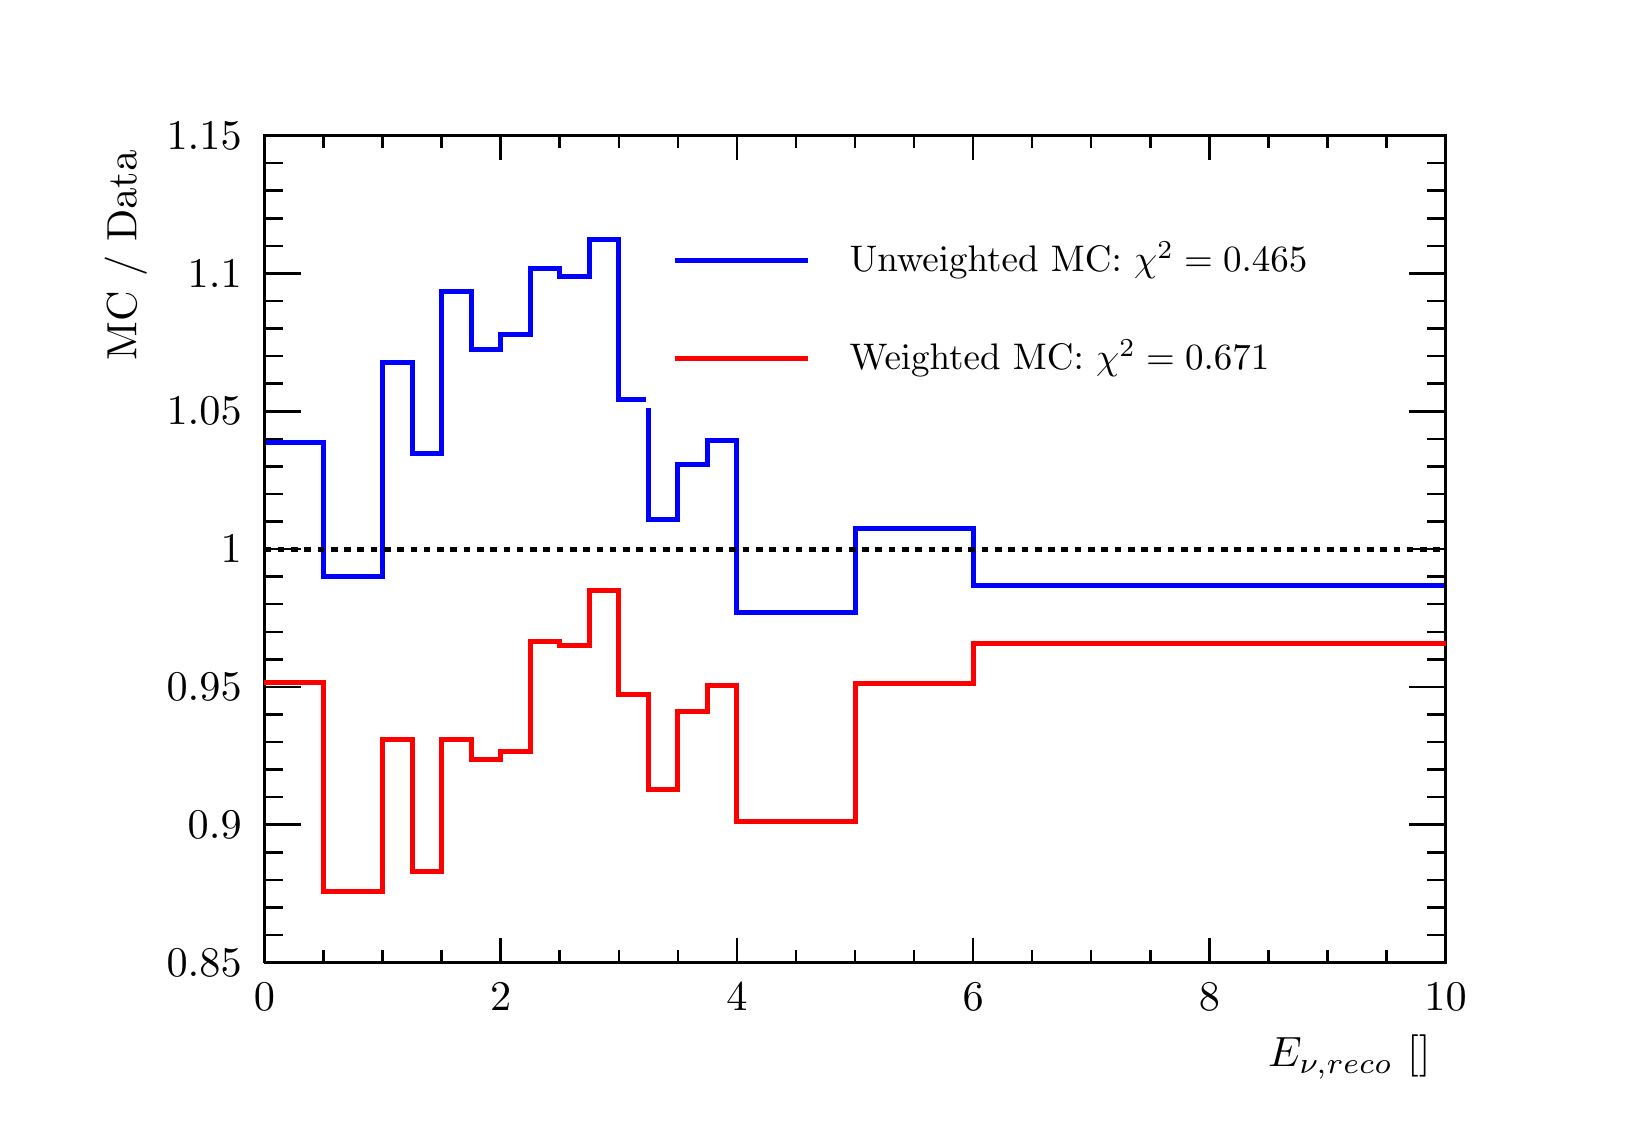
\begin{tikzpicture}
\pgfdeclareplotmark{cross} {
\pgfpathmoveto{\pgfpoint{-0.3\pgfplotmarksize}{\pgfplotmarksize}}
\pgfpathlineto{\pgfpoint{+0.3\pgfplotmarksize}{\pgfplotmarksize}}
\pgfpathlineto{\pgfpoint{+0.3\pgfplotmarksize}{0.3\pgfplotmarksize}}
\pgfpathlineto{\pgfpoint{+1\pgfplotmarksize}{0.3\pgfplotmarksize}}
\pgfpathlineto{\pgfpoint{+1\pgfplotmarksize}{-0.3\pgfplotmarksize}}
\pgfpathlineto{\pgfpoint{+0.3\pgfplotmarksize}{-0.3\pgfplotmarksize}}
\pgfpathlineto{\pgfpoint{+0.3\pgfplotmarksize}{-1.\pgfplotmarksize}}
\pgfpathlineto{\pgfpoint{-0.3\pgfplotmarksize}{-1.\pgfplotmarksize}}
\pgfpathlineto{\pgfpoint{-0.3\pgfplotmarksize}{-0.3\pgfplotmarksize}}
\pgfpathlineto{\pgfpoint{-1.\pgfplotmarksize}{-0.3\pgfplotmarksize}}
\pgfpathlineto{\pgfpoint{-1.\pgfplotmarksize}{0.3\pgfplotmarksize}}
\pgfpathlineto{\pgfpoint{-0.3\pgfplotmarksize}{0.3\pgfplotmarksize}}
\pgfpathclose
\pgfusepathqstroke
}
\pgfdeclareplotmark{cross*} {
\pgfpathmoveto{\pgfpoint{-0.3\pgfplotmarksize}{\pgfplotmarksize}}
\pgfpathlineto{\pgfpoint{+0.3\pgfplotmarksize}{\pgfplotmarksize}}
\pgfpathlineto{\pgfpoint{+0.3\pgfplotmarksize}{0.3\pgfplotmarksize}}
\pgfpathlineto{\pgfpoint{+1\pgfplotmarksize}{0.3\pgfplotmarksize}}
\pgfpathlineto{\pgfpoint{+1\pgfplotmarksize}{-0.3\pgfplotmarksize}}
\pgfpathlineto{\pgfpoint{+0.3\pgfplotmarksize}{-0.3\pgfplotmarksize}}
\pgfpathlineto{\pgfpoint{+0.3\pgfplotmarksize}{-1.\pgfplotmarksize}}
\pgfpathlineto{\pgfpoint{-0.3\pgfplotmarksize}{-1.\pgfplotmarksize}}
\pgfpathlineto{\pgfpoint{-0.3\pgfplotmarksize}{-0.3\pgfplotmarksize}}
\pgfpathlineto{\pgfpoint{-1.\pgfplotmarksize}{-0.3\pgfplotmarksize}}
\pgfpathlineto{\pgfpoint{-1.\pgfplotmarksize}{0.3\pgfplotmarksize}}
\pgfpathlineto{\pgfpoint{-0.3\pgfplotmarksize}{0.3\pgfplotmarksize}}
\pgfpathclose
\pgfusepathqfillstroke
}
\pgfdeclareplotmark{newstar} {
\pgfpathmoveto{\pgfqpoint{0pt}{\pgfplotmarksize}}
\pgfpathlineto{\pgfqpointpolar{44}{0.5\pgfplotmarksize}}
\pgfpathlineto{\pgfqpointpolar{18}{\pgfplotmarksize}}
\pgfpathlineto{\pgfqpointpolar{-20}{0.5\pgfplotmarksize}}
\pgfpathlineto{\pgfqpointpolar{-54}{\pgfplotmarksize}}
\pgfpathlineto{\pgfqpointpolar{-90}{0.5\pgfplotmarksize}}
\pgfpathlineto{\pgfqpointpolar{234}{\pgfplotmarksize}}
\pgfpathlineto{\pgfqpointpolar{198}{0.5\pgfplotmarksize}}
\pgfpathlineto{\pgfqpointpolar{162}{\pgfplotmarksize}}
\pgfpathlineto{\pgfqpointpolar{134}{0.5\pgfplotmarksize}}
\pgfpathclose
\pgfusepathqstroke
}
\pgfdeclareplotmark{newstar*} {
\pgfpathmoveto{\pgfqpoint{0pt}{\pgfplotmarksize}}
\pgfpathlineto{\pgfqpointpolar{44}{0.5\pgfplotmarksize}}
\pgfpathlineto{\pgfqpointpolar{18}{\pgfplotmarksize}}
\pgfpathlineto{\pgfqpointpolar{-20}{0.5\pgfplotmarksize}}
\pgfpathlineto{\pgfqpointpolar{-54}{\pgfplotmarksize}}
\pgfpathlineto{\pgfqpointpolar{-90}{0.5\pgfplotmarksize}}
\pgfpathlineto{\pgfqpointpolar{234}{\pgfplotmarksize}}
\pgfpathlineto{\pgfqpointpolar{198}{0.5\pgfplotmarksize}}
\pgfpathlineto{\pgfqpointpolar{162}{\pgfplotmarksize}}
\pgfpathlineto{\pgfqpointpolar{134}{0.5\pgfplotmarksize}}
\pgfpathclose
\pgfusepathqfillstroke
}
\definecolor{c}{rgb}{1,1,1};
\draw [color=c, fill=c] (0,0) rectangle (20,13.639);
\draw [color=c, fill=c] (3,1.77307) rectangle (18,12.2751);
\definecolor{c}{rgb}{0,0,0};
\draw [c,line width=0.9] (3,1.77307) -- (3,12.2751) -- (18,12.2751) -- (18,1.77307) -- (3,1.77307);
\definecolor{c}{rgb}{1,1,1};
\draw [color=c, fill=c] (3,1.77307) rectangle (18,12.2751);
\definecolor{c}{rgb}{0,0,0};
\draw [c,line width=0.9] (3,1.77307) -- (3,12.2751) -- (18,12.2751) -- (18,1.77307) -- (3,1.77307);
\definecolor{c}{rgb}{0,0,1};
\draw [c,line width=1.8] (3,8.3831) -- (3.75,8.3831) -- (3.75,6.67844) -- (4.5,6.67844) -- (4.5,9.3874) -- (4.875,9.3874) -- (4.875,8.24323) -- (5.25,8.24323) -- (5.25,10.2962) -- (5.625,10.2962) -- (5.625,9.5561) -- (6,9.5561) -- (6,9.75034) --
 (6.375,9.75034) -- (6.375,10.5885) -- (6.75,10.5885) -- (6.75,10.4817) -- (7.125,10.4817) -- (7.125,10.956) -- (7.5,10.956) -- (7.5,8.91923) -- (7.875,8.91923) -- (7.875,7.40592) -- (8.25,7.40592) -- (8.25,8.10331) -- (8.625,8.10331) --
 (8.625,8.40393) -- (9,8.40393) -- (9,6.22403) -- (10.5,6.22403) -- (10.5,7.29106) -- (12,7.29106) -- (12,6.56355) -- (18,6.56355);
\definecolor{c}{rgb}{0,0,0};
\draw [c,line width=0.9] (3,1.77307) -- (18,1.77307);
\draw [c,line width=0.9] (3,2.07994) -- (3,1.77307);
\draw [c,line width=0.9] (3.75,1.9265) -- (3.75,1.77307);
\draw [c,line width=0.9] (4.5,1.9265) -- (4.5,1.77307);
\draw [c,line width=0.9] (5.25,1.9265) -- (5.25,1.77307);
\draw [c,line width=0.9] (6,2.07994) -- (6,1.77307);
\draw [c,line width=0.9] (6.75,1.9265) -- (6.75,1.77307);
\draw [c,line width=0.9] (7.5,1.9265) -- (7.5,1.77307);
\draw [c,line width=0.9] (8.25,1.9265) -- (8.25,1.77307);
\draw [c,line width=0.9] (9,2.07994) -- (9,1.77307);
\draw [c,line width=0.9] (9.75,1.9265) -- (9.75,1.77307);
\draw [c,line width=0.9] (10.5,1.9265) -- (10.5,1.77307);
\draw [c,line width=0.9] (11.25,1.9265) -- (11.25,1.77307);
\draw [c,line width=0.9] (12,2.07994) -- (12,1.77307);
\draw [c,line width=0.9] (12.75,1.9265) -- (12.75,1.77307);
\draw [c,line width=0.9] (13.5,1.9265) -- (13.5,1.77307);
\draw [c,line width=0.9] (14.25,1.9265) -- (14.25,1.77307);
\draw [c,line width=0.9] (15,2.07994) -- (15,1.77307);
\draw [c,line width=0.9] (15.75,1.9265) -- (15.75,1.77307);
\draw [c,line width=0.9] (16.5,1.9265) -- (16.5,1.77307);
\draw [c,line width=0.9] (17.25,1.9265) -- (17.25,1.77307);
\draw [c,line width=0.9] (18,2.07994) -- (18,1.77307);
\draw [anchor=base] (3,1.15931) node[scale=1.52731, color=c, rotate=0]{0};
\draw [anchor=base] (6,1.15931) node[scale=1.52731, color=c, rotate=0]{2};
\draw [anchor=base] (9,1.15931) node[scale=1.52731, color=c, rotate=0]{4};
\draw [anchor=base] (12,1.15931) node[scale=1.52731, color=c, rotate=0]{6};
\draw [anchor=base] (15,1.15931) node[scale=1.52731, color=c, rotate=0]{8};
\draw [anchor=base] (18,1.15931) node[scale=1.52731, color=c, rotate=0]{10};
\draw [anchor= east] (18,0.572837) node[scale=1.52731, color=c, rotate=0]{$E_{\nu, \text{reco}}$ [\si{\GeV}]};
\draw [c,line width=0.9] (3,12.2751) -- (18,12.2751);
\draw [c,line width=0.9] (3,11.9682) -- (3,12.2751);
\draw [c,line width=0.9] (3.75,12.1216) -- (3.75,12.2751);
\draw [c,line width=0.9] (4.5,12.1216) -- (4.5,12.2751);
\draw [c,line width=0.9] (5.25,12.1216) -- (5.25,12.2751);
\draw [c,line width=0.9] (6,11.9682) -- (6,12.2751);
\draw [c,line width=0.9] (6.75,12.1216) -- (6.75,12.2751);
\draw [c,line width=0.9] (7.5,12.1216) -- (7.5,12.2751);
\draw [c,line width=0.9] (8.25,12.1216) -- (8.25,12.2751);
\draw [c,line width=0.9] (9,11.9682) -- (9,12.2751);
\draw [c,line width=0.9] (9.75,12.1216) -- (9.75,12.2751);
\draw [c,line width=0.9] (10.5,12.1216) -- (10.5,12.2751);
\draw [c,line width=0.9] (11.25,12.1216) -- (11.25,12.2751);
\draw [c,line width=0.9] (12,11.9682) -- (12,12.2751);
\draw [c,line width=0.9] (12.75,12.1216) -- (12.75,12.2751);
\draw [c,line width=0.9] (13.5,12.1216) -- (13.5,12.2751);
\draw [c,line width=0.9] (14.25,12.1216) -- (14.25,12.2751);
\draw [c,line width=0.9] (15,11.9682) -- (15,12.2751);
\draw [c,line width=0.9] (15.75,12.1216) -- (15.75,12.2751);
\draw [c,line width=0.9] (16.5,12.1216) -- (16.5,12.2751);
\draw [c,line width=0.9] (17.25,12.1216) -- (17.25,12.2751);
\draw [c,line width=0.9] (18,11.9682) -- (18,12.2751);
\draw [c,line width=0.9] (3,1.77307) -- (3,12.2751);
\draw [c,line width=0.9] (3.462,1.77307) -- (3,1.77307);
\draw [c,line width=0.9] (3.231,2.12313) -- (3,2.12313);
\draw [c,line width=0.9] (3.231,2.4732) -- (3,2.4732);
\draw [c,line width=0.9] (3.231,2.82327) -- (3,2.82327);
\draw [c,line width=0.9] (3.231,3.17333) -- (3,3.17333);
\draw [c,line width=0.9] (3.462,3.5234) -- (3,3.5234);
\draw [c,line width=0.9] (3.231,3.87347) -- (3,3.87347);
\draw [c,line width=0.9] (3.231,4.22353) -- (3,4.22353);
\draw [c,line width=0.9] (3.231,4.5736) -- (3,4.5736);
\draw [c,line width=0.9] (3.231,4.92367) -- (3,4.92367);
\draw [c,line width=0.9] (3.462,5.27373) -- (3,5.27373);
\draw [c,line width=0.9] (3.231,5.6238) -- (3,5.6238);
\draw [c,line width=0.9] (3.231,5.97387) -- (3,5.97387);
\draw [c,line width=0.9] (3.231,6.32394) -- (3,6.32394);
\draw [c,line width=0.9] (3.231,6.674) -- (3,6.674);
\draw [c,line width=0.9] (3.462,7.02407) -- (3,7.02407);
\draw [c,line width=0.9] (3.231,7.37414) -- (3,7.37414);
\draw [c,line width=0.9] (3.231,7.7242) -- (3,7.7242);
\draw [c,line width=0.9] (3.231,8.07427) -- (3,8.07427);
\draw [c,line width=0.9] (3.231,8.42434) -- (3,8.42434);
\draw [c,line width=0.9] (3.462,8.7744) -- (3,8.7744);
\draw [c,line width=0.9] (3.231,9.12447) -- (3,9.12447);
\draw [c,line width=0.9] (3.231,9.47454) -- (3,9.47454);
\draw [c,line width=0.9] (3.231,9.8246) -- (3,9.8246);
\draw [c,line width=0.9] (3.231,10.1747) -- (3,10.1747);
\draw [c,line width=0.9] (3.462,10.5247) -- (3,10.5247);
\draw [c,line width=0.9] (3.231,10.8748) -- (3,10.8748);
\draw [c,line width=0.9] (3.231,11.2249) -- (3,11.2249);
\draw [c,line width=0.9] (3.231,11.5749) -- (3,11.5749);
\draw [c,line width=0.9] (3.231,11.925) -- (3,11.925);
\draw [c,line width=0.9] (3.462,12.2751) -- (3,12.2751);
\draw [c,line width=0.9] (3.462,1.77307) -- (3,1.77307);
\draw [c,line width=0.9] (3.462,12.2751) -- (3,12.2751);
\draw [anchor= east] (2.9,1.77307) node[scale=1.52731, color=c, rotate=0]{0.85};
\draw [anchor= east] (2.9,3.5234) node[scale=1.52731, color=c, rotate=0]{0.9};
\draw [anchor= east] (2.9,5.27373) node[scale=1.52731, color=c, rotate=0]{0.95};
\draw [anchor= east] (2.9,7.02407) node[scale=1.52731, color=c, rotate=0]{1};
\draw [anchor= east] (2.9,8.7744) node[scale=1.52731, color=c, rotate=0]{1.05};
\draw [anchor= east] (2.9,10.5247) node[scale=1.52731, color=c, rotate=0]{1.1};
\draw [anchor= east] (2.9,12.2751) node[scale=1.52731, color=c, rotate=0]{1.15};
\draw [anchor= east] (1.24,12.2751) node[scale=1.52731, color=c, rotate=90]{MC / Data};
\draw [c,line width=0.9] (18,1.77307) -- (18,12.2751);
\draw [c,line width=0.9] (17.538,1.77307) -- (18,1.77307);
\draw [c,line width=0.9] (17.769,2.12313) -- (18,2.12313);
\draw [c,line width=0.9] (17.769,2.4732) -- (18,2.4732);
\draw [c,line width=0.9] (17.769,2.82327) -- (18,2.82327);
\draw [c,line width=0.9] (17.769,3.17333) -- (18,3.17333);
\draw [c,line width=0.9] (17.538,3.5234) -- (18,3.5234);
\draw [c,line width=0.9] (17.769,3.87347) -- (18,3.87347);
\draw [c,line width=0.9] (17.769,4.22353) -- (18,4.22353);
\draw [c,line width=0.9] (17.769,4.5736) -- (18,4.5736);
\draw [c,line width=0.9] (17.769,4.92367) -- (18,4.92367);
\draw [c,line width=0.9] (17.538,5.27373) -- (18,5.27373);
\draw [c,line width=0.9] (17.769,5.6238) -- (18,5.6238);
\draw [c,line width=0.9] (17.769,5.97387) -- (18,5.97387);
\draw [c,line width=0.9] (17.769,6.32394) -- (18,6.32394);
\draw [c,line width=0.9] (17.769,6.674) -- (18,6.674);
\draw [c,line width=0.9] (17.538,7.02407) -- (18,7.02407);
\draw [c,line width=0.9] (17.769,7.37414) -- (18,7.37414);
\draw [c,line width=0.9] (17.769,7.7242) -- (18,7.7242);
\draw [c,line width=0.9] (17.769,8.07427) -- (18,8.07427);
\draw [c,line width=0.9] (17.769,8.42434) -- (18,8.42434);
\draw [c,line width=0.9] (17.538,8.7744) -- (18,8.7744);
\draw [c,line width=0.9] (17.769,9.12447) -- (18,9.12447);
\draw [c,line width=0.9] (17.769,9.47454) -- (18,9.47454);
\draw [c,line width=0.9] (17.769,9.8246) -- (18,9.8246);
\draw [c,line width=0.9] (17.769,10.1747) -- (18,10.1747);
\draw [c,line width=0.9] (17.538,10.5247) -- (18,10.5247);
\draw [c,line width=0.9] (17.769,10.8748) -- (18,10.8748);
\draw [c,line width=0.9] (17.769,11.2249) -- (18,11.2249);
\draw [c,line width=0.9] (17.769,11.5749) -- (18,11.5749);
\draw [c,line width=0.9] (17.769,11.925) -- (18,11.925);
\draw [c,line width=0.9] (17.538,12.2751) -- (18,12.2751);
\draw [c,line width=0.9] (17.538,1.77307) -- (18,1.77307);
\draw [c,line width=0.9] (17.538,12.2751) -- (18,12.2751);
\definecolor{c}{rgb}{1,0,0};
\draw [c,line width=1.8] (3,5.33151) -- (3.75,5.33151) -- (3.75,2.67658) -- (4.5,2.67658) -- (4.5,4.60629) -- (4.875,4.60629) -- (4.875,2.93467) -- (5.25,2.93467) -- (5.25,4.60581) -- (5.625,4.60581) -- (5.625,4.35785) -- (6,4.35785) -- (6,4.44983)
 -- (6.375,4.44983) -- (6.375,5.84648) -- (6.75,5.84648) -- (6.75,5.79708) -- (7.125,5.79708) -- (7.125,6.49966) -- (7.5,6.49966) -- (7.5,5.17883) -- (7.875,5.17883) -- (7.875,3.96952) -- (8.25,3.96952) -- (8.25,4.96302) -- (8.625,4.96302) --
 (8.625,5.28866) -- (9,5.28866) -- (9,3.5664) -- (10.5,3.5664) -- (10.5,5.31798) -- (12,5.31798) -- (12,5.83084) -- (18,5.83084);
\definecolor{c}{rgb}{0,0,0};
\draw [c,dash pattern=on 2.40pt off 2.40pt ,line width=1.8] (3,7.02407) -- (18,7.02407);
\definecolor{c}{rgb}{1,1,1};
\draw [color=c, fill=c] (7.851,8.82522) rectangle (17.5072,11.3181);
\definecolor{c}{rgb}{0,0,0};
\draw [anchor= west] (10.265,10.6948) node[scale=1.3364, color=c, rotate=0]{Unweighted MC: $\chi^{2} = 0.465$};
\definecolor{c}{rgb}{0,0,1};
\draw [c,line width=1.8] (8.21311,10.6948) -- (9.90294,10.6948);
\definecolor{c}{rgb}{0,0,0};
\draw [anchor= west] (10.265,9.44842) node[scale=1.3364, color=c, rotate=0]{Weighted MC: $\chi^{2} = 0.671$};
\definecolor{c}{rgb}{1,0,0};
\draw [c,line width=1.8] (8.21311,9.44842) -- (9.90294,9.44842);
\definecolor{c}{rgb}{1,1,1};
\draw [color=c, fill=c] (2,12.8206) rectangle (18,13.5708);
\definecolor{c}{rgb}{0,0,0};
%\draw (10,13.1957) node[scale=1.40004, color=c, rotate=0]{Unweighted MC};
\end{tikzpicture}

		\end{adjustbox}
		\caption{RHC \anue}
	\end{subfigure}
	\caption[Ratio of weighted and unweighted far detector MC samples to `mock data']{Ratio of weighted and unweighted far detector MC samples to `mock data'. Additionally, for each sample, $\chi^{2}$ values are calculated for both MC samples and the `mock data' and displayed. Here, the true value of \dcp is $\pi$.}
	\label{fig:reweightedSamplesRatio}
\end{figure} 

Additionally, one can also see that differences remain between the weighted MC and `mock data'. 
These differences are the result of a number of different factors.

Firstly, the far detector events are reweighted on the basis of true \evis and \pvis and true final state.
These quantities do not correspond directly to the reconstructed quantities measured in ND-GAr and thus there will be deficiencies in the reweighting deriving from this.
However, it is not possible to reweight based upon the reconstructed energy of far detector events due to the differences in reconstruction techniques between ND-GAr and the FD.
Additionally, it may be more difficult in the FD to exclude energy carried by final neutrons from hadronic energy estimators.
A LAr TPC such as the FD may also find it more difficult to correctly identify final state pion multiplicities compared to ND-GAr, as shown in \citefig{fig:larConfusMat}.

Furthermore, many differences exist between the GENIE and NuWro which may not be encapsulated in the 3-dimensional reweighting space chosen.
An extension to further dimensions may mitigate these issues.
However, this approach relies on sufficient statistics in ND-GAr such that all parts of phase space are reasonably well populated.

\subsection{Bias reduction as a function of \dcp}
\label{sec:dune_ndrwt:rwt:biasReduction}

Far detector fits are performed at a variety of values of \dcp with the reweighted far detector samples as the MC.
\citefig{fig:dcpBiasWithWgt} shows the variation in the bias in the fitted value of \dcp as a function of $\delta_{CP, \text{true}}$ when using the reweighted MC.
The points made by using the unweighted MC are also included for comparison.
One can see that at most points, the bias on \dcp is lessened when the weighted MC is used.

\begin{figure}[h]
	\begin{adjustbox}{max totalsize=.6\linewidth, center}
		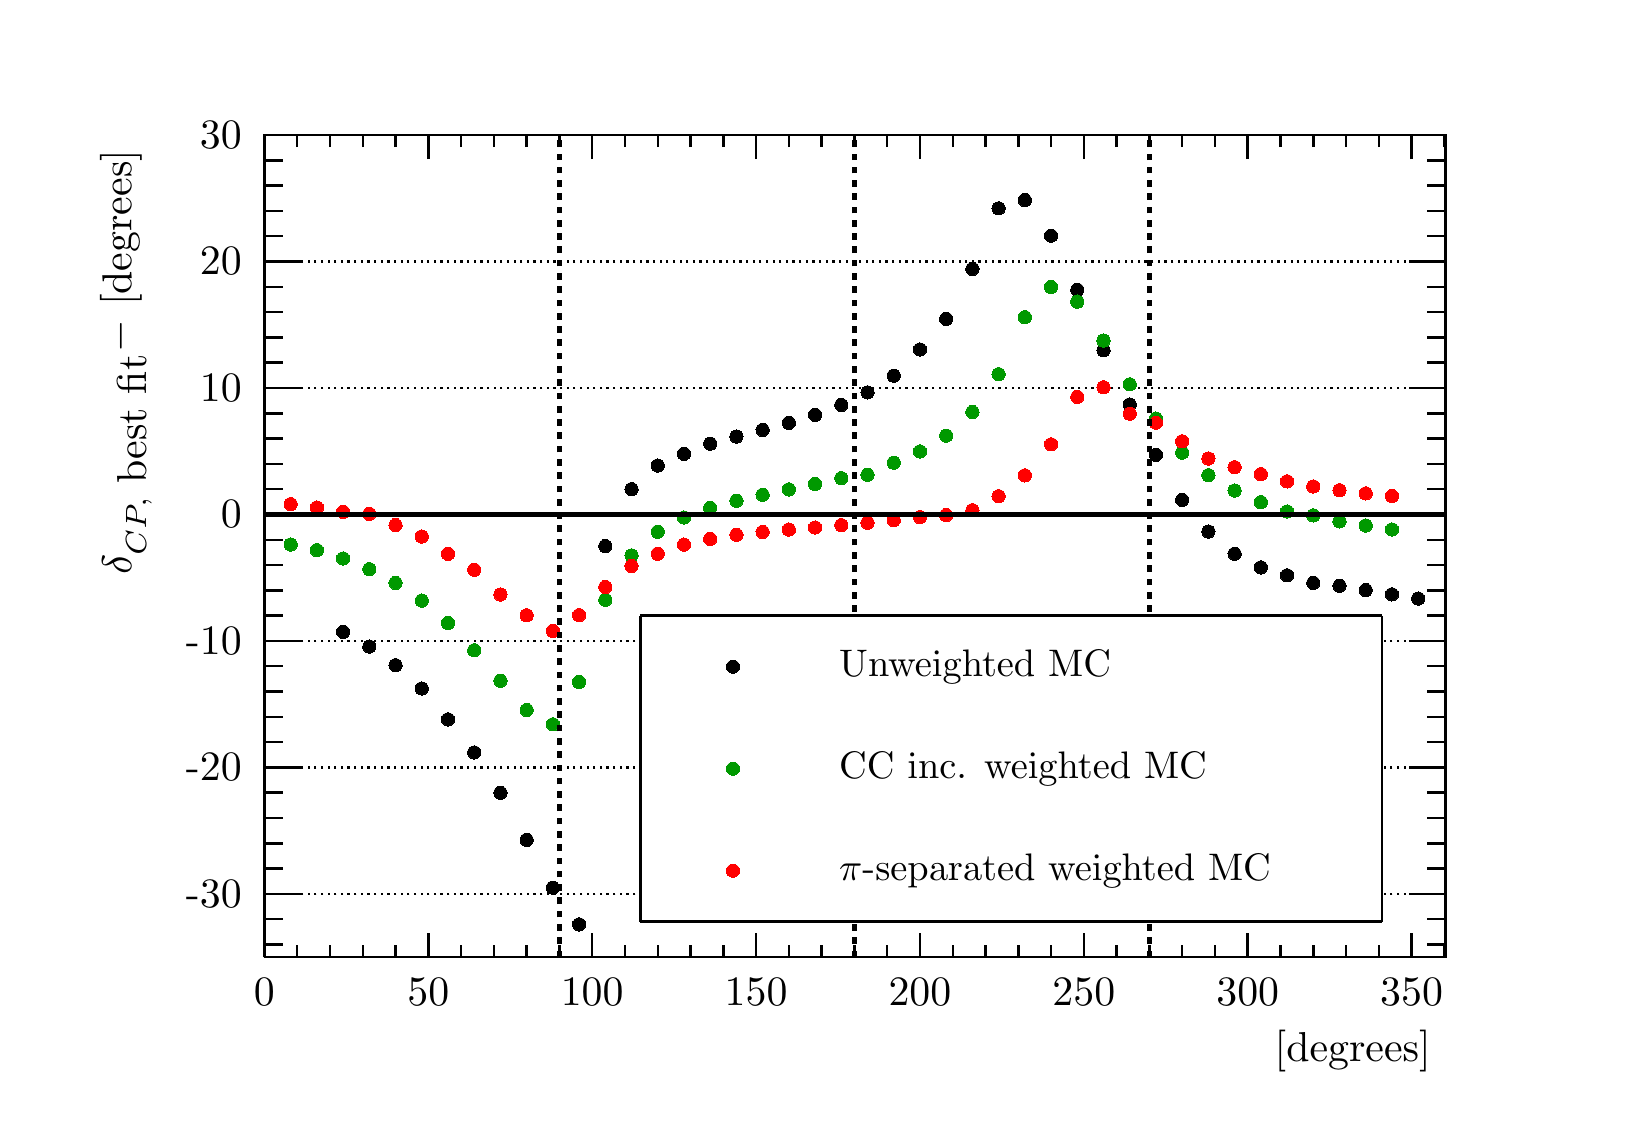
\begin{tikzpicture}
\pgfdeclareplotmark{cross} {
\pgfpathmoveto{\pgfpoint{-0.3\pgfplotmarksize}{\pgfplotmarksize}}
\pgfpathlineto{\pgfpoint{+0.3\pgfplotmarksize}{\pgfplotmarksize}}
\pgfpathlineto{\pgfpoint{+0.3\pgfplotmarksize}{0.3\pgfplotmarksize}}
\pgfpathlineto{\pgfpoint{+1\pgfplotmarksize}{0.3\pgfplotmarksize}}
\pgfpathlineto{\pgfpoint{+1\pgfplotmarksize}{-0.3\pgfplotmarksize}}
\pgfpathlineto{\pgfpoint{+0.3\pgfplotmarksize}{-0.3\pgfplotmarksize}}
\pgfpathlineto{\pgfpoint{+0.3\pgfplotmarksize}{-1.\pgfplotmarksize}}
\pgfpathlineto{\pgfpoint{-0.3\pgfplotmarksize}{-1.\pgfplotmarksize}}
\pgfpathlineto{\pgfpoint{-0.3\pgfplotmarksize}{-0.3\pgfplotmarksize}}
\pgfpathlineto{\pgfpoint{-1.\pgfplotmarksize}{-0.3\pgfplotmarksize}}
\pgfpathlineto{\pgfpoint{-1.\pgfplotmarksize}{0.3\pgfplotmarksize}}
\pgfpathlineto{\pgfpoint{-0.3\pgfplotmarksize}{0.3\pgfplotmarksize}}
\pgfpathclose
\pgfusepathqstroke
}
\pgfdeclareplotmark{cross*} {
\pgfpathmoveto{\pgfpoint{-0.3\pgfplotmarksize}{\pgfplotmarksize}}
\pgfpathlineto{\pgfpoint{+0.3\pgfplotmarksize}{\pgfplotmarksize}}
\pgfpathlineto{\pgfpoint{+0.3\pgfplotmarksize}{0.3\pgfplotmarksize}}
\pgfpathlineto{\pgfpoint{+1\pgfplotmarksize}{0.3\pgfplotmarksize}}
\pgfpathlineto{\pgfpoint{+1\pgfplotmarksize}{-0.3\pgfplotmarksize}}
\pgfpathlineto{\pgfpoint{+0.3\pgfplotmarksize}{-0.3\pgfplotmarksize}}
\pgfpathlineto{\pgfpoint{+0.3\pgfplotmarksize}{-1.\pgfplotmarksize}}
\pgfpathlineto{\pgfpoint{-0.3\pgfplotmarksize}{-1.\pgfplotmarksize}}
\pgfpathlineto{\pgfpoint{-0.3\pgfplotmarksize}{-0.3\pgfplotmarksize}}
\pgfpathlineto{\pgfpoint{-1.\pgfplotmarksize}{-0.3\pgfplotmarksize}}
\pgfpathlineto{\pgfpoint{-1.\pgfplotmarksize}{0.3\pgfplotmarksize}}
\pgfpathlineto{\pgfpoint{-0.3\pgfplotmarksize}{0.3\pgfplotmarksize}}
\pgfpathclose
\pgfusepathqfillstroke
}
\pgfdeclareplotmark{newstar} {
\pgfpathmoveto{\pgfqpoint{0pt}{\pgfplotmarksize}}
\pgfpathlineto{\pgfqpointpolar{44}{0.5\pgfplotmarksize}}
\pgfpathlineto{\pgfqpointpolar{18}{\pgfplotmarksize}}
\pgfpathlineto{\pgfqpointpolar{-20}{0.5\pgfplotmarksize}}
\pgfpathlineto{\pgfqpointpolar{-54}{\pgfplotmarksize}}
\pgfpathlineto{\pgfqpointpolar{-90}{0.5\pgfplotmarksize}}
\pgfpathlineto{\pgfqpointpolar{234}{\pgfplotmarksize}}
\pgfpathlineto{\pgfqpointpolar{198}{0.5\pgfplotmarksize}}
\pgfpathlineto{\pgfqpointpolar{162}{\pgfplotmarksize}}
\pgfpathlineto{\pgfqpointpolar{134}{0.5\pgfplotmarksize}}
\pgfpathclose
\pgfusepathqstroke
}
\pgfdeclareplotmark{newstar*} {
\pgfpathmoveto{\pgfqpoint{0pt}{\pgfplotmarksize}}
\pgfpathlineto{\pgfqpointpolar{44}{0.5\pgfplotmarksize}}
\pgfpathlineto{\pgfqpointpolar{18}{\pgfplotmarksize}}
\pgfpathlineto{\pgfqpointpolar{-20}{0.5\pgfplotmarksize}}
\pgfpathlineto{\pgfqpointpolar{-54}{\pgfplotmarksize}}
\pgfpathlineto{\pgfqpointpolar{-90}{0.5\pgfplotmarksize}}
\pgfpathlineto{\pgfqpointpolar{234}{\pgfplotmarksize}}
\pgfpathlineto{\pgfqpointpolar{198}{0.5\pgfplotmarksize}}
\pgfpathlineto{\pgfqpointpolar{162}{\pgfplotmarksize}}
\pgfpathlineto{\pgfqpointpolar{134}{0.5\pgfplotmarksize}}
\pgfpathclose
\pgfusepathqfillstroke
}
\definecolor{c}{rgb}{1,1,1};
\draw [color=c, fill=c] (0,0) rectangle (20,13.5603);
\draw [color=c, fill=c] (3,1.76284) rectangle (18,12.2043);
\definecolor{c}{rgb}{0,0,0};
\draw [c,line width=0.9] (3,1.76284) -- (3,12.2043) -- (18,12.2043) -- (18,1.76284) -- (3,1.76284);
\definecolor{c}{rgb}{1,1,1};
\draw [color=c, fill=c] (3,1.76284) rectangle (18,12.2043);
\definecolor{c}{rgb}{0,0,0};
\draw [c,line width=0.9] (3,1.76284) -- (3,12.2043) -- (18,12.2043) -- (18,1.76284) -- (3,1.76284);
\draw [c,line width=0.9] (3,1.76284) -- (18,1.76284);
\draw [c,line width=0.9] (3,12.2043) -- (18,12.2043);
\draw [c,line width=0.9] (3,1.76284) -- (3,12.2043);
\draw [c,dash pattern=on 0.80pt off 1.60pt ,line width=0.9] (18,2.56602) -- (3,2.56602);
\draw [c,dash pattern=on 0.80pt off 1.60pt ,line width=0.9] (18,4.17239) -- (3,4.17239);
\draw [c,dash pattern=on 0.80pt off 1.60pt ,line width=0.9] (18,5.77877) -- (3,5.77877);
\draw [c,dash pattern=on 0.80pt off 1.60pt ,line width=0.9] (18,7.38514) -- (3,7.38514);
\draw [c,dash pattern=on 0.80pt off 1.60pt ,line width=0.9] (18,8.99151) -- (3,8.99151);
\draw [c,dash pattern=on 0.80pt off 1.60pt ,line width=0.9] (18,10.5979) -- (3,10.5979);
\draw [c,dash pattern=on 0.80pt off 1.60pt ,line width=0.9] (18,12.2043) -- (3,12.2043);
\draw [c,dash pattern=on 0.80pt off 1.60pt ,line width=0.9] (18,2.56602) -- (3,2.56602);
\draw [c,line width=0.9] (18,1.76284) -- (18,12.2043);
\draw [c,line width=0.9] (3,1.76284) -- (18,1.76284);
\draw [c,line width=0.9] (3,2.06794) -- (3,1.76284);
\draw [c,line width=0.9] (3.41625,1.91539) -- (3.41625,1.76284);
\draw [c,line width=0.9] (3.8325,1.91539) -- (3.8325,1.76284);
\draw [c,line width=0.9] (4.24875,1.91539) -- (4.24875,1.76284);
\draw [c,line width=0.9] (4.665,1.91539) -- (4.665,1.76284);
\draw [c,line width=0.9] (5.08125,2.06794) -- (5.08125,1.76284);
\draw [c,line width=0.9] (5.4975,1.91539) -- (5.4975,1.76284);
\draw [c,line width=0.9] (5.91375,1.91539) -- (5.91375,1.76284);
\draw [c,line width=0.9] (6.33,1.91539) -- (6.33,1.76284);
\draw [c,line width=0.9] (6.74625,1.91539) -- (6.74625,1.76284);
\draw [c,line width=0.9] (7.1625,2.06794) -- (7.1625,1.76284);
\draw [c,line width=0.9] (7.57875,1.91539) -- (7.57875,1.76284);
\draw [c,line width=0.9] (7.99501,1.91539) -- (7.99501,1.76284);
\draw [c,line width=0.9] (8.41126,1.91539) -- (8.41126,1.76284);
\draw [c,line width=0.9] (8.82751,1.91539) -- (8.82751,1.76284);
\draw [c,line width=0.9] (9.24376,2.06794) -- (9.24376,1.76284);
\draw [c,line width=0.9] (9.66001,1.91539) -- (9.66001,1.76284);
\draw [c,line width=0.9] (10.0763,1.91539) -- (10.0763,1.76284);
\draw [c,line width=0.9] (10.4925,1.91539) -- (10.4925,1.76284);
\draw [c,line width=0.9] (10.9088,1.91539) -- (10.9088,1.76284);
\draw [c,line width=0.9] (11.325,2.06794) -- (11.325,1.76284);
\draw [c,line width=0.9] (11.7413,1.91539) -- (11.7413,1.76284);
\draw [c,line width=0.9] (12.1575,1.91539) -- (12.1575,1.76284);
\draw [c,line width=0.9] (12.5738,1.91539) -- (12.5738,1.76284);
\draw [c,line width=0.9] (12.99,1.91539) -- (12.99,1.76284);
\draw [c,line width=0.9] (13.4063,2.06794) -- (13.4063,1.76284);
\draw [c,line width=0.9] (13.8225,1.91539) -- (13.8225,1.76284);
\draw [c,line width=0.9] (14.2388,1.91539) -- (14.2388,1.76284);
\draw [c,line width=0.9] (14.655,1.91539) -- (14.655,1.76284);
\draw [c,line width=0.9] (15.0713,1.91539) -- (15.0713,1.76284);
\draw [c,line width=0.9] (15.4875,2.06794) -- (15.4875,1.76284);
\draw [c,line width=0.9] (15.9038,1.91539) -- (15.9038,1.76284);
\draw [c,line width=0.9] (16.32,1.91539) -- (16.32,1.76284);
\draw [c,line width=0.9] (16.7363,1.91539) -- (16.7363,1.76284);
\draw [c,line width=0.9] (17.1525,1.91539) -- (17.1525,1.76284);
\draw [c,line width=0.9] (17.5688,2.06794) -- (17.5688,1.76284);
\draw [c,line width=0.9] (17.5688,2.06794) -- (17.5688,1.76284);
\draw [c,line width=0.9] (17.985,1.91539) -- (17.985,1.76284);
\draw [anchor=base] (3,1.15262) node[scale=1.51215, color=c, rotate=0]{0};
\draw [anchor=base] (5.08125,1.15262) node[scale=1.51215, color=c, rotate=0]{50};
\draw [anchor=base] (7.1625,1.15262) node[scale=1.51215, color=c, rotate=0]{100};
\draw [anchor=base] (9.24376,1.15262) node[scale=1.51215, color=c, rotate=0]{150};
\draw [anchor=base] (11.325,1.15262) node[scale=1.51215, color=c, rotate=0]{200};
\draw [anchor=base] (13.4063,1.15262) node[scale=1.51215, color=c, rotate=0]{250};
\draw [anchor=base] (15.4875,1.15262) node[scale=1.51215, color=c, rotate=0]{300};
\draw [anchor=base] (17.5688,1.15262) node[scale=1.51215, color=c, rotate=0]{350};
\draw [anchor= east] (18,0.569532) node[scale=1.51215, color=c, rotate=0]{\dcpTrue [degrees]};
\draw [c,line width=0.9] (3,12.2043) -- (18,12.2043);
\draw [c,line width=0.9] (3,11.8991) -- (3,12.2043);
\draw [c,line width=0.9] (3.41625,12.0517) -- (3.41625,12.2043);
\draw [c,line width=0.9] (3.8325,12.0517) -- (3.8325,12.2043);
\draw [c,line width=0.9] (4.24875,12.0517) -- (4.24875,12.2043);
\draw [c,line width=0.9] (4.665,12.0517) -- (4.665,12.2043);
\draw [c,line width=0.9] (5.08125,11.8991) -- (5.08125,12.2043);
\draw [c,line width=0.9] (5.4975,12.0517) -- (5.4975,12.2043);
\draw [c,line width=0.9] (5.91375,12.0517) -- (5.91375,12.2043);
\draw [c,line width=0.9] (6.33,12.0517) -- (6.33,12.2043);
\draw [c,line width=0.9] (6.74625,12.0517) -- (6.74625,12.2043);
\draw [c,line width=0.9] (7.1625,11.8991) -- (7.1625,12.2043);
\draw [c,line width=0.9] (7.57875,12.0517) -- (7.57875,12.2043);
\draw [c,line width=0.9] (7.99501,12.0517) -- (7.99501,12.2043);
\draw [c,line width=0.9] (8.41126,12.0517) -- (8.41126,12.2043);
\draw [c,line width=0.9] (8.82751,12.0517) -- (8.82751,12.2043);
\draw [c,line width=0.9] (9.24376,11.8991) -- (9.24376,12.2043);
\draw [c,line width=0.9] (9.66001,12.0517) -- (9.66001,12.2043);
\draw [c,line width=0.9] (10.0763,12.0517) -- (10.0763,12.2043);
\draw [c,line width=0.9] (10.4925,12.0517) -- (10.4925,12.2043);
\draw [c,line width=0.9] (10.9088,12.0517) -- (10.9088,12.2043);
\draw [c,line width=0.9] (11.325,11.8991) -- (11.325,12.2043);
\draw [c,line width=0.9] (11.7413,12.0517) -- (11.7413,12.2043);
\draw [c,line width=0.9] (12.1575,12.0517) -- (12.1575,12.2043);
\draw [c,line width=0.9] (12.5738,12.0517) -- (12.5738,12.2043);
\draw [c,line width=0.9] (12.99,12.0517) -- (12.99,12.2043);
\draw [c,line width=0.9] (13.4063,11.8991) -- (13.4063,12.2043);
\draw [c,line width=0.9] (13.8225,12.0517) -- (13.8225,12.2043);
\draw [c,line width=0.9] (14.2388,12.0517) -- (14.2388,12.2043);
\draw [c,line width=0.9] (14.655,12.0517) -- (14.655,12.2043);
\draw [c,line width=0.9] (15.0713,12.0517) -- (15.0713,12.2043);
\draw [c,line width=0.9] (15.4875,11.8991) -- (15.4875,12.2043);
\draw [c,line width=0.9] (15.9038,12.0517) -- (15.9038,12.2043);
\draw [c,line width=0.9] (16.32,12.0517) -- (16.32,12.2043);
\draw [c,line width=0.9] (16.7363,12.0517) -- (16.7363,12.2043);
\draw [c,line width=0.9] (17.1525,12.0517) -- (17.1525,12.2043);
\draw [c,line width=0.9] (17.5688,11.8991) -- (17.5688,12.2043);
\draw [c,line width=0.9] (17.5688,11.8991) -- (17.5688,12.2043);
\draw [c,line width=0.9] (17.985,12.0517) -- (17.985,12.2043);
\draw [c,line width=0.9] (3,1.76284) -- (3,12.2043);
\draw [c,line width=0.9] (3.462,2.56602) -- (3,2.56602);
\draw [c,line width=0.9] (3.231,2.8873) -- (3,2.8873);
\draw [c,line width=0.9] (3.231,3.20857) -- (3,3.20857);
\draw [c,line width=0.9] (3.231,3.52985) -- (3,3.52985);
\draw [c,line width=0.9] (3.231,3.85112) -- (3,3.85112);
\draw [c,line width=0.9] (3.462,4.17239) -- (3,4.17239);
\draw [c,line width=0.9] (3.231,4.49367) -- (3,4.49367);
\draw [c,line width=0.9] (3.231,4.81494) -- (3,4.81494);
\draw [c,line width=0.9] (3.231,5.13622) -- (3,5.13622);
\draw [c,line width=0.9] (3.231,5.45749) -- (3,5.45749);
\draw [c,line width=0.9] (3.462,5.77877) -- (3,5.77877);
\draw [c,line width=0.9] (3.231,6.10004) -- (3,6.10004);
\draw [c,line width=0.9] (3.231,6.42132) -- (3,6.42132);
\draw [c,line width=0.9] (3.231,6.74259) -- (3,6.74259);
\draw [c,line width=0.9] (3.231,7.06386) -- (3,7.06386);
\draw [c,line width=0.9] (3.462,7.38514) -- (3,7.38514);
\draw [c,line width=0.9] (3.231,7.70641) -- (3,7.70641);
\draw [c,line width=0.9] (3.231,8.02769) -- (3,8.02769);
\draw [c,line width=0.9] (3.231,8.34896) -- (3,8.34896);
\draw [c,line width=0.9] (3.231,8.67024) -- (3,8.67024);
\draw [c,line width=0.9] (3.462,8.99151) -- (3,8.99151);
\draw [c,line width=0.9] (3.231,9.31279) -- (3,9.31279);
\draw [c,line width=0.9] (3.231,9.63406) -- (3,9.63406);
\draw [c,line width=0.9] (3.231,9.95533) -- (3,9.95533);
\draw [c,line width=0.9] (3.231,10.2766) -- (3,10.2766);
\draw [c,line width=0.9] (3.462,10.5979) -- (3,10.5979);
\draw [c,line width=0.9] (3.231,10.9192) -- (3,10.9192);
\draw [c,line width=0.9] (3.231,11.2404) -- (3,11.2404);
\draw [c,line width=0.9] (3.231,11.5617) -- (3,11.5617);
\draw [c,line width=0.9] (3.231,11.883) -- (3,11.883);
\draw [c,line width=0.9] (3.462,12.2043) -- (3,12.2043);
\draw [c,line width=0.9] (3.462,2.56602) -- (3,2.56602);
\draw [c,line width=0.9] (3.231,2.24475) -- (3,2.24475);
\draw [c,line width=0.9] (3.231,1.92347) -- (3,1.92347);
\draw [anchor= east] (2.9,2.56602) node[scale=1.51215, color=c, rotate=0]{-30};
\draw [anchor= east] (2.9,4.17239) node[scale=1.51215, color=c, rotate=0]{-20};
\draw [anchor= east] (2.9,5.77877) node[scale=1.51215, color=c, rotate=0]{-10};
\draw [anchor= east] (2.9,7.38514) node[scale=1.51215, color=c, rotate=0]{0};
\draw [anchor= east] (2.9,8.99151) node[scale=1.51215, color=c, rotate=0]{10};
\draw [anchor= east] (2.9,10.5979) node[scale=1.51215, color=c, rotate=0]{20};
\draw [anchor= east] (2.9,12.2043) node[scale=1.51215, color=c, rotate=0]{30};
\draw [anchor= east] (1.24,12.2043) node[scale=1.51215, color=c, rotate=90]{$\delta_{CP,~\textrm{best fit}} - \dcpTrue$ [degrees]};
\draw [c,line width=0.9] (18,1.76284) -- (18,12.2043);
\draw [c,line width=0.9] (17.538,2.56602) -- (18,2.56602);
\draw [c,line width=0.9] (17.769,2.8873) -- (18,2.8873);
\draw [c,line width=0.9] (17.769,3.20857) -- (18,3.20857);
\draw [c,line width=0.9] (17.769,3.52985) -- (18,3.52985);
\draw [c,line width=0.9] (17.769,3.85112) -- (18,3.85112);
\draw [c,line width=0.9] (17.538,4.17239) -- (18,4.17239);
\draw [c,line width=0.9] (17.769,4.49367) -- (18,4.49367);
\draw [c,line width=0.9] (17.769,4.81494) -- (18,4.81494);
\draw [c,line width=0.9] (17.769,5.13622) -- (18,5.13622);
\draw [c,line width=0.9] (17.769,5.45749) -- (18,5.45749);
\draw [c,line width=0.9] (17.538,5.77877) -- (18,5.77877);
\draw [c,line width=0.9] (17.769,6.10004) -- (18,6.10004);
\draw [c,line width=0.9] (17.769,6.42132) -- (18,6.42132);
\draw [c,line width=0.9] (17.769,6.74259) -- (18,6.74259);
\draw [c,line width=0.9] (17.769,7.06386) -- (18,7.06386);
\draw [c,line width=0.9] (17.538,7.38514) -- (18,7.38514);
\draw [c,line width=0.9] (17.769,7.70641) -- (18,7.70641);
\draw [c,line width=0.9] (17.769,8.02769) -- (18,8.02769);
\draw [c,line width=0.9] (17.769,8.34896) -- (18,8.34896);
\draw [c,line width=0.9] (17.769,8.67024) -- (18,8.67024);
\draw [c,line width=0.9] (17.538,8.99151) -- (18,8.99151);
\draw [c,line width=0.9] (17.769,9.31279) -- (18,9.31279);
\draw [c,line width=0.9] (17.769,9.63406) -- (18,9.63406);
\draw [c,line width=0.9] (17.769,9.95533) -- (18,9.95533);
\draw [c,line width=0.9] (17.769,10.2766) -- (18,10.2766);
\draw [c,line width=0.9] (17.538,10.5979) -- (18,10.5979);
\draw [c,line width=0.9] (17.769,10.9192) -- (18,10.9192);
\draw [c,line width=0.9] (17.769,11.2404) -- (18,11.2404);
\draw [c,line width=0.9] (17.769,11.5617) -- (18,11.5617);
\draw [c,line width=0.9] (17.769,11.883) -- (18,11.883);
\draw [c,line width=0.9] (17.538,12.2043) -- (18,12.2043);
\draw [c,line width=0.9] (17.538,2.56602) -- (18,2.56602);
\draw [c,line width=0.9] (17.769,2.24475) -- (18,2.24475);
\draw [c,line width=0.9] (17.769,1.92347) -- (18,1.92347);
\foreach \P in {(3.999,5.89376), (4.332,5.70739), (4.665,5.4712), (4.998,5.1748), (5.331,4.78284), (5.664,4.36308), (5.997,3.8498), (6.33,3.25239), (6.663,2.64556), (6.996,2.17921), (7.329,6.98376), (7.662,7.70655), (7.99501,8.00579),
 (8.32801,8.15546), (8.66101,8.28375), (8.99401,8.37416), (9.32701,8.4587), (9.66001,8.54915), (9.99301,8.6505), (10.326,8.77565), (10.659,8.93528), (10.992,9.14738), (11.325,9.48058), (11.658,9.86968), (11.991,10.5031), (12.324,11.2726),
 (12.657,11.3777), (12.99,10.925), (13.323,10.2384), (13.656,9.4696), (13.989,8.78134), (14.322,8.14301), (14.655,7.56952), (14.988,7.1674), (15.321,6.88575), (15.654,6.71275), (15.987,6.6118), (16.32,6.5165), (16.653,6.47938), (16.986,6.42435),
 (17.319,6.3704), (17.652,6.3169)}{\draw[mark options={color=c,fill=c},mark size=2.402402pt, line width=0.000000pt, mark=*] plot coordinates {\P};}
\definecolor{c}{rgb}{1,1,1};
\draw [color=c, fill=c] (2,12.7467) rectangle (18,13.4925);
\definecolor{c}{rgb}{0,0,0};
%\draw (10,13.1196) node[scale=1.38614, color=c, rotate=0]{Unweighted MC};
\definecolor{c}{rgb}{0,0.6,0};
\foreach \P in {(3.333,7.00321), (3.666,6.93165), (3.999,6.82615), (4.332,6.69018), (4.665,6.5158), (4.998,6.29084), (5.331,6.00512), (5.664,5.66082), (5.997,5.27369), (6.33,4.90165), (6.663,4.72004), (6.996,5.25847), (7.329,6.30145),
 (7.662,6.86524), (7.99501,7.16582), (8.32801,7.34643), (8.66101,7.46856), (8.99401,7.55965), (9.32701,7.63485), (9.66001,7.70337), (9.99301,7.7716), (10.326,7.8461), (10.659,7.8886), (10.992,8.04253), (11.325,8.18552), (11.658,8.38589),
 (11.991,8.68617), (12.324,9.16637), (12.657,9.89039), (12.99,10.2729), (13.323,10.0878), (13.656,9.5933), (13.989,9.03807), (14.322,8.60232), (14.655,8.17044), (14.988,7.88401), (15.321,7.68859), (15.654,7.54124), (15.987,7.42269), (16.32,7.37364),
 (16.653,7.29735), (16.986,7.24452), (17.319,7.19439)}{\draw[mark options={color=c,fill=c},mark size=2.402402pt, line width=0.000000pt, mark=*] plot coordinates {\P};}
\definecolor{c}{rgb}{1,0,0};
\foreach \P in {(3.333,7.51624), (3.666,7.47326), (3.999,7.41876), (4.332,7.39304), (4.665,7.25022), (4.998,7.1046), (5.331,6.88581), (5.664,6.68283), (5.997,6.36882), (6.33,6.10472), (6.663,5.90619), (6.996,6.10632), (7.329,6.46369),
 (7.662,6.73066), (7.99501,6.88634), (8.32801,7.0018), (8.66101,7.07409), (8.99401,7.12634), (9.32701,7.16291), (9.66001,7.19333), (9.99301,7.2192), (10.326,7.24928), (10.659,7.27962), (10.992,7.31358), (11.325,7.351), (11.658,7.37707),
 (11.991,7.43904), (12.324,7.61704), (12.657,7.88169), (12.99,8.27566), (13.323,8.87789), (13.656,9.00015), (13.989,8.66472), (14.322,8.54999), (14.655,8.3143), (14.988,8.09578), (15.321,7.9855), (15.654,7.89718), (15.987,7.80543), (16.32,7.74059),
 (16.653,7.69268), (16.986,7.65291), (17.319,7.61818)}{\draw[mark options={color=c,fill=c},mark size=2.402402pt, line width=0.000000pt, mark=*] plot coordinates {\P};}
\definecolor{c}{rgb}{0,0,0};
\draw [c,line width=1.8] (3,7.38514) -- (17.985,7.38514);
\draw [c,dash pattern=on 2.40pt off 2.40pt ,line width=1.8] (6.74625,1.76284) -- (6.74625,12.2043);
\draw [c,dash pattern=on 2.40pt off 2.40pt ,line width=1.8] (10.4925,1.76284) -- (10.4925,12.2043);
\draw [c,dash pattern=on 2.40pt off 2.40pt ,line width=1.8] (14.2388,1.76284) -- (14.2388,12.2043);
\definecolor{c}{rgb}{1,1,1};
\draw [color=c, fill=c] (7.77305,2.21277) rectangle (17.1915,6.09929);
\definecolor{c}{rgb}{0,0,0};
\draw [c,line width=0.9] (7.77305,2.21277) -- (17.1915,2.21277);
\draw [c,line width=0.9] (17.1915,2.21277) -- (17.1915,6.09929);
\draw [c,line width=0.9] (17.1915,6.09929) -- (7.77305,6.09929);
\draw [c,line width=0.9] (7.77305,6.09929) -- (7.77305,2.21277);
\draw [anchor= west] (10.1277,5.45154) node[scale=1.38614, color=c, rotate=0]{Unweighted MC};
\foreach \P in {(8.95035,5.45154)}{\draw[mark options={color=c,fill=c},mark size=2.402402pt, line width=0.000000pt, mark=*] plot coordinates {\P};}
\draw [anchor= west] (10.1277,4.15603) node[scale=1.38614, color=c, rotate=0]{CC inc. weighted MC};
\definecolor{c}{rgb}{0,0.6,0};
\foreach \P in {(8.95035,4.15603)}{\draw[mark options={color=c,fill=c},mark size=2.402402pt, line width=0.000000pt, mark=*] plot coordinates {\P};}
\definecolor{c}{rgb}{0,0,0};
\draw [anchor= west] (10.1277,2.86052) node[scale=1.38614, color=c, rotate=0]{$\pi$-separated weighted MC};
\definecolor{c}{rgb}{1,0,0};
\foreach \P in {(8.95035,2.86052)}{\draw[mark options={color=c,fill=c},mark size=2.402402pt, line width=0.000000pt, mark=*] plot coordinates {\P};}
\end{tikzpicture}

	\end{adjustbox}
	\caption[Bias in fit value of \dcp with ND-GAr reweighted MC]{Bias in the measured value of \dcp as a function of the true value of \dcp. Points for both the nominal GENIE MC and the reweighted MC are shown.}
	\label{fig:dcpBiasWithWgt}
\end{figure}
